\documentclass[11pt,a4paper]{article}
\usepackage[utf8]{inputenc}
\usepackage[T1]{fontenc}
\usepackage[ngerman]{babel}
\usepackage{lmodern,amsmath,amssymb,longtable,pdflscape,tikz,graphicx}
\usepackage[protrusion=false,expansion=false]{microtype}
\usepackage[margin=20mm]{geometry}
\usepackage[unicode,hidelinks]{hyperref}
\pdfglyphtounicode{tfm:lmex10/parenleftbig}{0028}
\pdfglyphtounicode{tfm:lmex10/parenrightbig}{0029}
\pdfglyphtounicode{tfm:lmex10/braceleftbig}{007B}
\pdfglyphtounicode{tfm:lmex10/bracerightbig}{007D}
\pdfglyphtounicode{tfm:lmex10/summationdisplay}{2211}
\pdfglyphtounicode{tfm:lmex10/bracketleftBig}{005B}
\pdfglyphtounicode{tfm:lmex10/bracketleftbig}{005B}
\pdfglyphtounicode{tfm:lmex10/bracketrightBig}{005D}
\pdfglyphtounicode{tfm:lmex10/parenleftBig}{0028}
\pdfglyphtounicode{tfm:lmex10/parenrightBig}{0029}
\pdfglyphtounicode{tfm:lmex10/parenleftbigg}{0028}
\pdfglyphtounicode{tfm:lmex10/parenrightbigg}{0029}
\pdfglyphtounicode{tfm:lmex10/parenleftBigg}{0028}
\pdfglyphtounicode{tfm:lmex10/parenrightBigg}{0029}
\pdfglyphtounicode{tfm:lmex10/bracketrightbig}{005D}
\pdfglyphtounicode{tfm:lmex10/bracketleftbigg}{005B}
\pdfglyphtounicode{tfm:lmex10/bracketrightbigg}{005D}
\pdfglyphtounicode{tfm:lmex10/bracketleftBigg}{005B}
\pdfglyphtounicode{tfm:lmex10/bracketrightBigg}{005D}
\pdfglyphtounicode{tfm:lmex10/braceleftBig}{007B}
\pdfglyphtounicode{tfm:lmex10/bracerightBig}{007D}
\pdfglyphtounicode{tfm:lmex10/braceleftbigg}{007B}
\pdfglyphtounicode{tfm:lmex10/bracerightbigg}{007D}
\pdfglyphtounicode{tfm:lmex10/braceleftBigg}{007B}
\pdfglyphtounicode{tfm:lmex10/bracerightBigg}{007D}
\pdfglyphtounicode{tfm:eufm10/A}{D835 DD04}
\pdfglyphtounicode{tfm:eufm10/B}{D835 DD05}
\pdfglyphtounicode{tfm:eufm10/C}{212D}
\pdfglyphtounicode{tfm:eufm10/D}{D835 DD07}
\pdfglyphtounicode{tfm:eufm10/E}{D835 DD08}
\pdfglyphtounicode{tfm:eufm10/F}{D835 DD09}
\pdfglyphtounicode{tfm:eufm10/x}{D835 DD35}
\pdfglyphtounicode{tfm:eufm10/Y}{D835 DD1C}
\pdfglyphtounicode{tfm:eufm10/Z}{2128}
\pdfglyphtounicode{tfm:lmex10/radicalBig}{221A}
\pdfglyphtounicode{tfm:lmex10/radicalbig}{221A}
\pdfglyphtounicode{tfm:lmex10/radicalBigg}{221A}
\pdfglyphtounicode{tfm:lmex10/radicalbigg}{221A}
\pdfglyphtounicode{tfm:lmex10/integraltext}{222B}
\pdfglyphtounicode{tfm:lmex10/integraldisplay}{222B}
% IX Oldenburg equations (2) and (4): logical text for assembled curly braces.
% Display-style aligned bodies only. The marked spans contain no formula text.
\newbox\GaussOldenburgBraceBody
\newbox\GaussOldenburgBraceMeasure
\newcommand{\GaussOldenburgMarkedBrace}[3]{%
  \pdfliteral direct{/Span << /ActualText <FEFF#1> >> BDC}%
  \hbox{$\nulldelimiterspace=0pt\relax
    \displaystyle\left#2\copy\GaussOldenburgBraceMeasure\right#3$}%
  \pdfliteral direct{EMC}%
}
\newcommand{\GaussOldenburgBraceAssembly}[2]{%
  \mathinner{\hbox{%
    \mathsurround=0pt\relax
    \setbox\GaussOldenburgBraceBody=\hbox{$\displaystyle#1$}%
    \setbox\GaussOldenburgBraceMeasure=\hbox{}%
    \ht\GaussOldenburgBraceMeasure=\ht\GaussOldenburgBraceBody
    \dp\GaussOldenburgBraceMeasure=\dp\GaussOldenburgBraceBody
    \GaussOldenburgMarkedBrace{007B}{\{}{.}%
    \copy\GaussOldenburgBraceBody
    #2%
  }}%
}
\newcommand{\GaussOldenburgBracePair}[1]{%
  \GaussOldenburgBraceAssembly{#1}{\GaussOldenburgMarkedBrace{007D}{.}{\}}}%
}
\newcommand{\GaussOldenburgLeftBrace}[1]{%
  \GaussOldenburgBraceAssembly{#1}{\kern\nulldelimiterspace}%
}


\newcommand{\GaussRightBrace}[1]{%
  \mathinner{\hbox{%
    \mathsurround=0pt\relax
    \setbox\GaussOldenburgBraceBody=\hbox{$\displaystyle#1$}%
    \setbox\GaussOldenburgBraceMeasure=\hbox{}%
    \ht\GaussOldenburgBraceMeasure=\ht\GaussOldenburgBraceBody
    \dp\GaussOldenburgBraceMeasure=\dp\GaussOldenburgBraceBody
    \kern\nulldelimiterspace
    \copy\GaussOldenburgBraceBody
    \GaussOldenburgMarkedBrace{007D}{.}{\}}%
  }}%
}

\newcommand{\GaussSquareBracketPair}[1]{%
  \mathinner{\hbox{%
    \mathsurround=0pt\relax
    \setbox\GaussOldenburgBraceBody=\hbox{$\displaystyle#1$}%
    \setbox\GaussOldenburgBraceMeasure=\hbox{}%
    \ht\GaussOldenburgBraceMeasure=\ht\GaussOldenburgBraceBody
    \dp\GaussOldenburgBraceMeasure=\dp\GaussOldenburgBraceBody
    \GaussOldenburgMarkedBrace{005B}{[}{.}%
    \copy\GaussOldenburgBraceBody
    \GaussOldenburgMarkedBrace{005D}{.}{]}%
  }}%
}


\hypersetup{pdftitle={Carl Friedrich Gauss, Werke IX: Geodätische Schriften},
pdfauthor={Carl Friedrich Gauss; Louis Krüger und Anton Börsch (historische Bemerkungen)}}
\pagestyle{empty}
\setlength{\parindent}{1.5em}
\newcommand{\GaussIXMathCopy}[2]{%
  \pdfliteral direct{/Span << /ActualText (#1) >> BDC}#2\pdfliteral direct{EMC}%
}
\begin{document}
\begin{center}
{\Large Carl Friedrich Gauss\par}\medskip
{\LARGE Werke, Band IX\par}\bigskip
{\large Geodätische Schriften\par}\medskip
Übertragung in modernes Deutsch\par
\end{center}
\section*{Zu dieser Übersetzung}
\noindent Carl Friedrich Gauss, \textit{Werke}, Band IX, \textit{Geodäsie. Fortsetzung von Band IV}. Die Königliche Gesellschaft der Wissenschaften zu Göttingen gab die historische Ausgabe 1903 heraus. Sie erschien in Kommission bei B. G. Teubner in Leipzig. L. Krüger bearbeitete den Band mit Unterstützung von A. Börsch. M. Brendel leitete die allgemeine Redaktion.

Diese Übertragung ins heutige Deutsch umfasst den historischen Vorspann und S.~1--528 mit der hannoverschen Faltkarte und der Verlagsanzeige. OpenAI GPT-6.1 Sol (Ultra) fertigte die KI-Übersetzung und den Satz auf Grundlage der editierbaren Transkription der Ausgabe von 1903 an. Die Urheberschaft der historischen Texte, der Anmerkungen und der Abbildungen ist im Band ausgewiesen, soweit sie bekannt ist.

\noindent\hyperlink{gaussix-sources}{Quellen und Textanmerkungen}

\begingroup
\clearpage\thispagestyle{empty}
\noindent\makebox[\linewidth][c]{%
\begin{tikzpicture}
\draw[line width=.65pt] (0,0) rectangle (\textwidth,224mm);
\draw[line width=.3pt] (6mm,6mm) rectangle (\textwidth-6mm,218mm);
\node[anchor=north,inner sep=0pt,text width=\dimexpr\textwidth-16mm\relax,align=center] at (.5\textwidth,197mm) {%
{\Large\bfseries CARL FRIEDRICH GAUSS}\par\vspace{12mm}
{\Huge\bfseries WERKE}\par\vspace{16mm}
{\large\textls[200]{NEUNTER BAND}}\par\vspace{17mm}
{\footnotesize HERAUSGEGEBEN}\par\vspace{8mm}
{\scriptsize VON DER}\par\vspace{9mm}
{\normalsize\bfseries KÖNIGLICHEN GESELLSCHAFT DER WISSENSCHAFTEN}\par\vspace{7mm}
{\scriptsize ZU}\par\vspace{6mm}
{\large\textls[180]{GÖTTINGEN}}\par\vspace{28mm}
{\small IN KOMMISSION BEI B. G. TEUBNER IN LEIPZIG}\par\vspace{3mm}
{\small 1903.}};
\end{tikzpicture}}\par
\clearpage\null
\clearpage\thispagestyle{empty}
\vspace*{76mm}
\begin{center}
{\Large CARL FRIEDRICH GAUSS WERKE}\par\vspace{12mm}
{\large BAND IX.}
\end{center}
\clearpage\null
\clearpage\thispagestyle{empty}
\begin{center}
\vspace*{10mm}
{\Large CARL FRIEDRICH GAUSS}\par\vspace{10mm}
{\Huge\bfseries WERKE}\par\vspace{14mm}
{\large\textls[200]{NEUNTER BAND.}}\par\vspace{11mm}
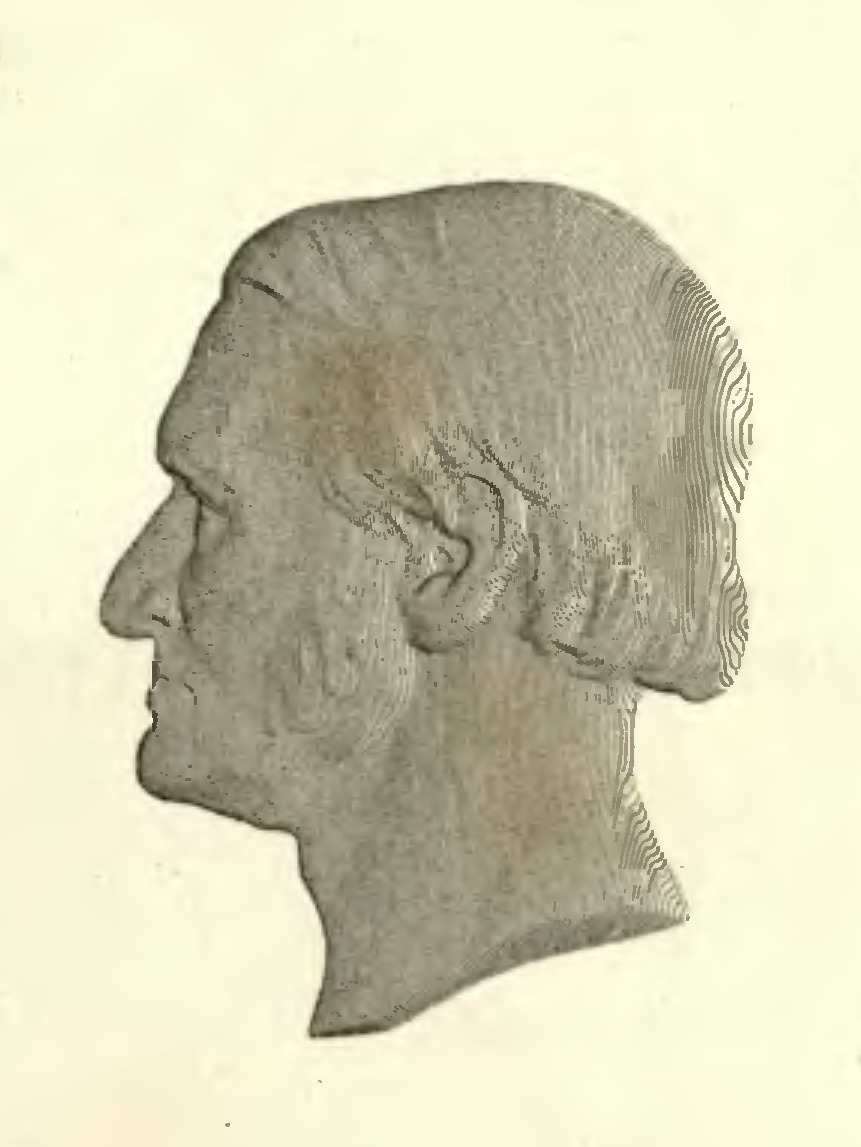
\includegraphics[trim=12bp 14bp 14bp 27bp,clip,width=44mm]{gauss_title_vignette_1870.jpg}\par\vspace{18mm}
{\footnotesize HERAUSGEGEBEN}\par\vspace{3mm}
{\scriptsize VON DER}\par\vspace{3mm}
{\small KÖNIGLICHEN GESELLSCHAFT DER WISSENSCHAFTEN}\par\vspace{3mm}
{\scriptsize ZU}\par\vspace{4mm}
{\large\textls[180]{GÖTTINGEN.}}\par\vspace{3mm}
{\small IN KOMMISSION BEI B. G. TEUBNER IN LEIPZIG.}\par\vspace{3mm}
{\small 1903.}
\end{center}
\clearpage\null
\endgroup

\clearpage
\begin{center}
{\Large BESTIMMUNG}\par\vspace{8mm}
{\small DES}\par\vspace{8mm}
{\LARGE\textls[100]{BREITENUNTERSCHIEDS}}\par\vspace{8mm}
{\small ZWISCHEN DEN}\par\vspace{7mm}
{\large STERNWARTEN VON GÖTTINGEN UND ALTONA}\par\vspace{7mm}
{\small DURCH}\par\vspace{7mm}
{\normalsize BEOBACHTUNGEN MIT DEM RAMSDENSCHEN ZENITSEKTOR}\par\vspace{7mm}
{\small VON}\par\vspace{7mm}
{\large\textls[100]{CARL FRIEDRICH GAUSS,}}\par\smallskip
{\scriptsize
RITTER DES GUELPHEN- UND DANNEBROG-ORDENS; KÖNIGLICH GROSSBRITANNISCH-HANNOVERSCHER HOFRAT;\\
PROFESSOR DER ASTRONOMIE UND DIREKTOR DER STERNWARTE IN GÖTTINGEN;\\
MITGLIED DER AKADEMIEN UND SOZIETÄTEN VON BERLIN, KOPENHAGEN, EDINBURGH, GÖTTINGEN,
LONDON, MÜNCHEN, NEAPEL, PARIS, PETERSBURG UND STOCKHOLM SOWIE DER
AMERIKANISCHEN, ITALIENISCHEN, KURLÄNDISCHEN, LONDONER ASTRONOMISCHEN U. A.
}\par\vspace{15mm}
\rule{.35\textwidth}{.4pt}\par\medskip
{\large\textls[170]{GÖTTINGEN,}}\par\medskip
BEI VANDENHOECK UND RUPRECHT.\par\medskip
1828.
\end{center}
\vfill\noindent IX.\hfill 1\par

\clearpage
\null

\clearpage
\begin{center}
{\LARGE\textls[170]{INHALT.}}\par\medskip
\rule{.09\textwidth}{.4pt}
\end{center}
\noindent Einleitung\dotfill S.\quad 5\par
\noindent\makebox[8mm][r]{I.}\quad Die beobachteten Sterne.\dotfill \quotedblbase\quad 8\par
\noindent\makebox[8mm][r]{II.}\quad Die Beobachtungen\dotfill \quotedblbase\quad 10\par
\noindent\makebox[8mm][r]{III.}\quad Ergebnisse\dotfill \quotedblbase\quad 29\par
\noindent\hspace*{12mm}\begin{minipage}{\dimexpr\textwidth-24mm\relax}
Einfachste Kombination der Beobachtungen zur Bestimmung des Breitenunterschieds, Art.\ 1.
Genauigkeit der Beobachtungen, Art.\ 2. Kollimationsfehler, Art.\ 3.
Absolut vorteilhafteste Kombination der Beobachtungen, Art.\ 4---7.
Berücksichtigung der unregelmäßigen Teilungsfehler, Art.\ 8---11. Lage der Beobachtungsplätze, Art.\ 12.
Bestimmung der absoluten Polhöhe der Göttinger Sternwarte aus Beobachtungen des Polarsterns
am \textsc{Reichenbach}schen Meridiankreis, Art.\ 13---17. Endergebnis der hannoverschen
Gradmessung, Art.\ 18---20. Vergleich der Deklinationen der beobachteten Zenitsterne mit den
Bestimmungen von \textsc{Bradley} und \textsc{Piazzi}, Art.\ 21.
\end{minipage}\par
\noindent\makebox[8mm][r]{IV.}\quad Breitenbestimmung der Sternwarte Seeberg\dotfill \quotedblbase\quad 52\par
\noindent Zusatz zu [Art.\ 20] S.\ 48\dotfill \quotedblbase\quad 56\par
\begin{center}\rule{.23\textwidth}{.4pt}\end{center}
\vfill\begin{flushright}$1^{\ast}$\end{flushright}

\clearpage
\null

\clearpage
\vspace*{12mm}
\begin{center}
{\large BESTIMMUNG DES BREITENUNTERSCHIEDS}\par\medskip
{\small ZWISCHEN}\par\medskip
{\large DEN STERNWARTEN VON GÖTTINGEN UND ALTONA\\
DURCH BEOBACHTUNGEN\\
MIT DEM RAMSDENSCHEN ZENITSEKTOR.}\par\medskip
\rule{.12\textwidth}{.4pt}\par\bigskip
{\large EINLEITUNG.}
\end{center}

Durch die Dreieckskette, die ich in den Jahren 1821---1824 durch das Königreich Hannover
entlang des Göttinger Meridians geführt habe, sind die Sternwarten von Göttingen und Altona
mit größter Genauigkeit trigonometrisch miteinander verbunden. Diese Messungen werden
später ausführlich veröffentlicht. Hier sei nur bemerkt, dass die absoluten Größen
auf der von Herrn Professor \textsc{Schumacher} in Holstein mit äußerster Genauigkeit
gemessenen Basis beruhen, mit der das Dreieckssystem durch die Seite Hamburg-Hohenhorn
verbunden ist. Die Orientierung stützt sich auf die Beobachtungen mit dem Göttinger
Passagenfernrohr, da die Sternwarte und das nördliche Meridianzeichen selbst Dreieckspunkte
sind. Die Sternwarten von Göttingen und Altona liegen durch einen merkwürdigen Zufall
bis auf weniger als eine Hausbreite auf demselben Meridian. Obwohl die absoluten Polhöhen
durch Beobachtungen mit fest aufgestellten Meridianinstrumenten bestimmt sind, war es
doch wichtig, den Breitenunterschied noch auf eine andere Weise mit ein und demselben
Instrument zu bestimmen, und ich hatte das Glück,

\clearpage
\noindent\makebox[10mm][l]{6}\parbox[t]{\dimexpr\textwidth-10mm\relax}{\centering\scriptsize BESTIMMUNG DES\,\quotedblbase\,BREITENUNTERSCHIEDS ZWISCHEN GÖTTINGEN UND ALTONA.}\par
\noindent dazu den ausgezeichneten Zenitsektor von \textsc{Ramsden} verwenden zu können,
der bekanntlich bei der englischen Gradmessung einem ähnlichen Zweck gedient hat.
Die Beobachtungen, die ich damit im Frühjahr 1827 angestellt habe, und ihre Ergebnisse
sind der Hauptgegenstand dieser Schrift.

Wenn viele Sterne nacheinander zu beobachten sind, lassen sich die Beobachtungen mit diesem
Instrument kaum ohne die Hilfe eines geübten Assistenten ausführen. Herr Professor
\textsc{Schumacher} hatte daher die Güte, Herrn Ingenieurleutnant von
\textsc{Nehus}[\textsuperscript{*})] mit Genehmigung Seiner Majestät des Königs von Dänemark
für die Beobachtungen an beiden Orten damit zu beauftragen. Dieser sehr geschickte Beobachter
übernahm fortlaufend das Ablesen der Mikrometerschraube und das Einstellen des Lotfadens.
Ich selbst beobachtete die Durchgänge an den Meridianfäden und stellte den zum Meridian
senkrechten Faden auf die Sterne ein. Nur in den beiden ersten Beobachtungsnächten in Altona
übernahm ein anderer Assistent jene Aufgabe. Deshalb habe ich diese Beobachtungen nicht
aufgenommen, zumal die Erfahrung bestätigte, dass verschiedene Personen die Halbierung
der Punkte durch den Lotfaden unterschiedlich einschätzten.

Das Instrument ist durch die ausführliche Beschreibung von \textsc{Mudge} hinreichend
bekannt. In Göttingen konnte es in der Sternwarte selbst unter dem östlichen Meridianspalt
aufgestellt werden. In Altona war das nicht möglich. Daher wurde es im Garten von Herrn
Professor \textsc{Schumacher}, in dem die dortige Sternwarte selbst steht, unter demselben
Beobachtungszelt aufgestellt, das \textsc{Mudge} in England benutzt hatte. Die Stabilität der
Aufstellung auf eingerammten Pfählen ließ nichts zu wünschen übrig. Die Nivellierung der
Vertikalachse wurde täglich überprüft, und gewöhnlich war fast nichts zu ändern. Dasselbe
gilt für die Horizontalachse.

Um die Ebene des Teilkreises in den Meridian zu bringen, wurde in Göttingen das südliche
Meridianzeichen benutzt. Es steht zwar im Meridian des westlichen Spalts, doch ließ sich sein
Azimut am Standort des Sektors mit größter Genauigkeit berechnen. In Altona ließ sich kein
ähnliches Verfahren anwenden. Dort wurde der Teilkreis zunächst mithilfe der bekannten
absoluten Zeit anhand eines kulminierenden Sterns sehr nahe in den

\vfill\noindent\rule{.24\textwidth}{.4pt}\par
{\footnotesize\noindent [\textsuperscript{*}) Handschriftliche Bemerkung:] \textsc{Nehus} starb am 17. April 1844 an zurückgetretener Grippe.\par}

\clearpage
\noindent\mbox{}\hfill EINLEITUNG.\hfill 7\par
\noindent Meridian gebracht. Durch Beobachtung mehrerer Sterne über die ganze Ausdehnung
des Teilkreises ließ sich dann leicht die noch nötige kleine Korrektur der Einstellung
bestimmen. Wie bereits erwähnt, wurden jede Nacht auch die Durchgänge der am Sektor
kulminierenden Sterne an den Meridianfäden beobachtet, und die Rektaszensionen der Sterne
waren bekannt. Damit ließ sich die richtige Ausrichtung im Meridian fortwährend zuverlässig
überprüfen. Nur einmal war eine geringfügige Nachstellung nötig. In der Regel wechselte
von einer Nacht zur nächsten die Stellung des Teilkreises zwischen Ost und West. Nur gegen
Ende der Beobachtungen wurde von dieser Regel gelegentlich abgewichen, um die Zahl der
Beobachtungen auf beide Lagen annähernd gleich zu verteilen. Dann wurde der Sektor in
einer Nacht einmal oder mehrmals gewendet.

Die Anzeigen des Barometers sowie des Innen- und Außenthermometers wurden jede Nacht
mindestens dreimal aufgezeichnet, zu Beginn, in der Mitte und am Ende der Beobachtungen.
Nach dem Vorbild von \textsc{Mudge} wurde ebenso der Temperaturunterschied zwischen dem
oberen und unteren Ende des Sektors aufgezeichnet, da er den Teilkreis und den Radius
in ungleichem Verhältnis verändert. Dass im Übrigen jede weitere durch die Bauart des
Instruments vorgeschriebene Vorsichtsmaßnahme sorgfältig beachtet wurde, braucht wohl
nicht eigens erwähnt zu werden. Dazu gehörte etwa, das Wassergefäß, in das das Lot hängt,
ausreichend gefüllt zu halten und möglichst dieselben Gewindegänge der Mikrometerschraube
zu benutzen. Bei jedem Stern wurde der Lotfaden unabhängig von der vorhergehenden Einstellung
neu auf den oberen Punkt (den Mittelpunkt des Gradbogens) eingestellt. Die Einstellung
auf den nächsten Teilungspunkt (oder die beiden nächsten) wurde in der Regel mehrmals
wiederholt. Aus den verschiedenen Ablesungen der Mikrometerschraube, die meistens bis auf
wenige Dezimalbruchteile einer Sekunde übereinstimmten, wurde der Mittelwert gebildet.

\begin{center}\rule{.24\textwidth}{.4pt}\end{center}

\clearpage
\vspace*{18mm}
\begin{center}
{\large I.}\par\medskip
{\Large DIE BEOBACHTETEN STERNE.}
\end{center}

Anfangs hatte ich 38 Sterne in für die Beobachtung geeigneten Lagen ausgewählt.
Gegen Ende der Beobachtungen in Göttingen fügte ich noch fünf weitere hinzu, weil ich
befürchtete, ungünstiges Wetter könnte den Abschluss der Beobachtungen in Altona so weit
verzögern, dass ein beträchtlicher Teil der zuerst ausgewählten Sterne wegen ihrer dann
tagsüber eintretenden Kulmination nicht oft genug beobachtet werden könnte. Diese Befürchtung
bestätigte sich jedoch nur in geringem Maße, und nur ein einziger Stern wurde in Altona bloß
einseitig beobachtet. Ich gebe hier die mittlere Stellung dieser Sterne, reduziert auf den
Anfang des Jahres 1827. Die Deklinationen sind die Ergebnisse der Beobachtungen mit dem
Zenitsektor selbst. Die Rektaszensionen, deren genaueste Bestimmung für den vorliegenden
Zweck unwesentlich ist, beruhen meist nur auf einer einmaligen Beobachtung am Meridiankreis,
deren Reduktion Herr \textsc{von Heiligenstein} freundlicherweise berechnet hat.
Der Bequemlichkeit halber bezeichne ich die Sterne mit fortlaufenden Nummern. Nr.\ 8, 13, 15
und 31 sind Doppelsterne. Beim ersten wurde stets der nachfolgende Stern eingestellt, bei
den beiden folgenden die Mitte. Bei Nr.\ 31 ist der Begleitstern so lichtschwach, dass er
im Fernrohr des Sektors selbst bei versuchsweise verdunkeltem Gesichtsfeld stets unsichtbar
blieb. Herr Professor \textsc{Schumacher} bemerkte ihn dagegen im lichtstärkeren Fernrohr
des \textsc{Reichenbach}schen Meridiankreises sofort, obwohl uns damals nicht bekannt war,
dass andere Astronomen diesen Stern bereits als Doppelstern erkannt hatten.

\clearpage
\noindent\parbox[t]{\dimexpr\textwidth-10mm\relax}{\centering\scriptsize BESTIMMUNG DES BREITENUNTERSCHIEDS USW.\quad I.\quad DIE BEOBACHTETEN STERNE.}\makebox[10mm][r]{9}\par
\begin{center}
\begin{minipage}[t]{.49\textwidth}\centering
{\scriptsize\setlength{\tabcolsep}{1.2pt}\renewcommand{\arraystretch}{1.2}\begin{tabular}{r|l|rrr|rrr|}
\multicolumn{2}{c|}{Bezeichnung}&\multicolumn{3}{c|}{Rektasz. 1827}&\multicolumn{3}{c|}{Dekl. 1827}\\\hline
1&24 Canum&$13^{\mathrm h}$&$27^{\mathrm m}$&$22^{\mathrm s}{,}39$&$49^\circ$&$54'$&$11''{,}62$\\
2&83 Ursae&&$34$&$9{,}77$&$55$&$33$&$34{,}98$\\
3&$\eta$ Ursae&&$40$&$42{,}86$&$50$&$10$&$46{,}20$\\
4&86 Ursae&&$47$&$28{,}48$&$54$&$34$&$55{,}55$\\
5&&&$50$&$45{,}55$&$55$&$25$&$59{,}22$\\
6&P. 13. 289&&$55$&$19{,}44$&$46$&$35$&$39{,}14$\\
7&13 Bootis&$14$&$1$&$49{,}02$&$50$&$16$&$43{,}44$\\
8&$\varkappa$ Bootis seq.&&$7$&$16{,}93$&$52$&$36$&$7{,}47$\\
9&P. 14. 56&&$12$&$5{,}39$&$56$&$13$&$36{,}51$\\
10&$\theta$ Bootis&&$19$&$18{,}40$&$52$&$39$&$12{,}05$\\
11&P. 14. 131&&$27$&$50{,}42$&$53$&$39$&$33{,}02$\\
12&P. 14. 164&&$35$&$24{,}18$&$52$&$58$&$55{,}66$\\
13&39 Bootis med.&&$43$&$48{,}37$&$49$&$26$&$9{,}46$\\
14&P. 14. 235&&$50$&$38{,}71$&$50$&$20$&$22{,}49$\\
15&44 Bootis med.&&$58$&$5{,}30$&$48$&$19$&$52{,}47$\\
16&&$15$&$7$&$8{,}12$&$49$&$13$&$46{,}68$\\
17&P. 15. 39&&$10$&$33{,}95$&$51$&$34$&$53{,}72$\\
18&&&$15$&$0{,}55$&$52$&$35$&$5{,}87$\\
19&&&$21$&$50{,}88$&$54$&$37$&$34{,}87$\\
20&&&$30$&$42{,}13$&$54$&$29$&$54{,}30$\\
21&&&$38$&$9{,}07$&$52$&$54$&$37{,}09$\\
22&&&$42$&$14{,}32$&$46$&$16$&$4{,}70$\\
\end{tabular}}\end{minipage}\hfill
\begin{minipage}[t]{.49\textwidth}\centering
{\scriptsize\setlength{\tabcolsep}{1.2pt}\renewcommand{\arraystretch}{1.2}\begin{tabular}{r|l|rrr|rrr}
\multicolumn{2}{c|}{Bezeichnung}&\multicolumn{3}{c|}{Rektasz. 1827}&\multicolumn{3}{c|}{Dekl. 1827}\\\hline
23&&$15^{\mathrm h}$&$48^{\mathrm m}$&$16^{\mathrm s}{,}24$&$56^\circ$&$20'$&$27''{,}00$\\
24&&&$54$&$10{,}23$&$50$&$22$&$39{,}41$\\
25&$\theta$ Draconis&&$58$&$39{,}70$&$59$&$1$&$47{,}14$\\
26&&$16$&$4$&$24{,}06$&$50$&$38$&$13{,}12$\\
27&P. 16. 33&&$7$&$24{,}92$&$46$&$20$&$17{,}04$\\
28&P. 16. 56&&$11$&$34{,}31$&$53$&$40$&$13{,}41$\\
29&&&$16$&$2{,}19$&$52$&$27$&$11{,}06$\\
30&&&$20$&$38{,}75$&$55$&$36$&$4{,}73$\\
31&&&$26$&$34{,}90$&$45$&$58$&$5{,}85$\\
32&16 Draconis&&$32$&$6{,}42$&$53$&$15$&$3{,}64$\\
33&&&$37$&$53{,}85$&$50$&$16$&$13{,}67$\\
34&&&$42$&$1{,}51$&$57$&$5$&$37{,}79$\\
35&&&$45$&$2{,}26$&$46$&$56$&$48{,}53$\\
36&P. 16. 253&&$49$&$21{,}51$&$46$&$49$&$22{,}01$\\
37&P. 16. 291&&$56$&$11{,}73$&$56$&$56$&$42{,}35$\\
38&P. 16. 310&$17$&$0$&$15{,}10$&$49$&$2$&$47{,}09$\\
39&P. 17. 20&&$4$&$23{,}12$&$58$&$29$&$49{,}33$\\
40&P. 17. 38&&$8$&$1{,}46$&$56$&$52$&$21{,}74$\\
41&74 Herculis&&$15$&$28{,}30$&$46$&$24$&$52{,}90$\\
42&P. 17. 120&&$20$&$53{,}56$&$57$&$10$&$13{,}11$\\
43&$\beta$ Draconis&&$26$&$31{,}90$&$52$&$25$&$57{,}91$\\
&&&&&&&\\
\end{tabular}}\end{minipage}
\end{center}
\begin{center}\rule{.24\textwidth}{.4pt}\end{center}

\clearpage
\vspace*{18mm}
\begin{center}
{\large II.}\par\medskip
{\Large DIE BEOBACHTUNGEN.}
\end{center}

Ein vollständiger Abdruck des Tagebuchs in seiner ursprünglichen Form hätte den Umfang
dieser Schrift mehr als verdoppelt und schien mir überflüssig. Ich gebe daher die
Beobachtungen sogleich nach Sternen geordnet wieder.

Die erste Spalte enthält die Zenitdistanzen, wie sie das Instrument geliefert hat,
das heißt die bloße Reduktion der Ablesung. Nördliche Zenitdistanzen gelten als positiv,
südliche als negativ.

Die zweite Spalte gibt die gemeinsame Wirkung der Refraktion und der ungleichen Ausdehnung
des Instruments infolge des Temperaturunterschieds zwischen dem oberen und dem unteren Teil
an. Die größten vorgekommenen Unterschiede waren $+1^\circ{,}2$ Réaum.\ (das obere
Thermometer zeigte mehr an) und $-0^\circ{,}6$. Um ein unverfälschtes Ergebnis zur
Beurteilung der gegenseitigen Übereinstimmung der Beobachtungen zu erhalten, habe ich die
Mühe nicht gescheut, den Betrag für jede einzelne Beobachtung zu berechnen. Dabei habe ich
einige kleine, sich leicht anbietende Rechenvorteile genutzt.

Die dritte Spalte enthält die Reduktion auf den mittleren Ort zu Jahresbeginn wegen
Aberration, Nutation und Präzession. Bei einigen Sternen kommt noch die Eigenbewegung hinzu.
Für die jährliche Eigenbewegung in Deklination wurde nämlich angenommen:
\begin{center}
\begin{tabular}{@{}lr@{\quad}c@{\quad}l@{}}
für&10&.\ .\ .\ .\ .\ .\ .&$-0''{,}42$\\
&25&.\ .\ .\ .\ .\ .\ .&$+0{,}33$\\
&37&.\ .\ .\ .\ .\ .\ .&$+0{,}38$.
\end{tabular}
\end{center}

\clearpage
\noindent\parbox[t]{\dimexpr\textwidth-10mm\relax}{\centering\scriptsize BESTIMMUNG DES BREITENUNTERSCHIEDS USW.\quad II.\quad DIE BEOBACHTUNGEN.}\makebox[10mm][r]{11}\par
\noindent Bei den beiden ersten Sternen steht die Eigenbewegung seit Langem fest. Bei Nr.\ 37
zeigt sie sich beim Vergleich mit der Bestimmung von \textsc{Piazzi} so, dass sie nicht zu
bezweifeln ist, sofern diese Bestimmung richtig ist\textsuperscript{*}). Der Berechnung
der Aberration, Nutation und Präzession liegen die wertvollen Tafeln von \textsc{Baily}
zugrunde. Nach ihnen wurde für jeden Stern mit Unterstützung der Herren von
\textsc{Nehus} und \textsc{Petersen} eine Ephemeride in Abständen von zehn Tagen berechnet
und darin unter Berücksichtigung der zweiten Differenzen interpoliert.

Die vierte Spalte enthält schließlich die Summe der ersten drei, also die wahre,
nur noch mit dem Kollimationsfehler behaftete Zenitdistanz für die mittlere Stellung
zu Beginn des Jahres 1827, wie sie sich aus jeder einzelnen Beobachtung ergibt.

\medskip\noindent\rule{.24\textwidth}{.4pt}\par
{\footnotesize
\noindent\textsuperscript{*}) Die Richtigkeit der auf 8 Beobachtungen beruhenden Bestimmung
dieses Sterns durch \textsc{Piazzi} wird durch die enge Übereinstimmung mit der Angabe in der
älteren Ausgabe seines Verzeichnisses von 1803 bestätigt, die auf 6 Beobachtungen beruhte.
Die genaue Größe der Eigenbewegung bleibt dennoch etwas ungewiss, weil das Jahr, das dem
Mittel der Beobachtungen entspricht, unbekannt ist. Es ist bemerkenswert, eine derart
beträchtliche Eigenbewegung bei einem Stern 7.\ Größe zu finden. Auch Nr.\ 11 scheint in
dieser Hinsicht die Aufmerksamkeit der Astronomen zu verdienen.\par}
\begin{center}\rule{.24\textwidth}{.4pt}\end{center}

\begingroup
\setlength{\arraycolsep}{2.2pt}
\setlength{\tabcolsep}{0pt}
\renewcommand{\arraystretch}{1.00}
\def\ixStar#1{\par\noindent\hfill{\normalsize\textls[80]{#1}}\hfill\null\par\smallskip}
\footnotesize

% Printed 12; principal PDF 19; Google PDF 23.
\par\clearpage
\noindent\makebox[12mm][l]{\fontsize{13}{16}\selectfont 12}\parbox[t]{\dimexpr\linewidth-24mm\relax}{\centering\scriptsize\bfseries BESTIMMUNG DES BREITENUNTERSCHIEDS ZWISCHEN GÖTTINGEN UND ALTONA.}\makebox[12mm][r]{}\par\medskip

\vspace*{.19\textheight}
\ixStar{1.\quad (24 Canum Venaticorum)}
\noindent\begin{tabular}{@{}c@{\hspace{.4em}\vrule width .65pt\hspace{.4em}}c@{}}
\multicolumn{1}{@{}c@{\hspace{.8em}}}{\makebox[.48\linewidth][c]{\normalsize Göttingen.\quad Teilkreis Ost.}} &
\multicolumn{1}{@{}c@{}}{\makebox[.48\linewidth][c]{\normalsize Göttingen.\quad Teilkreis West.}} \\[.18ex]
\(\begin{array}[t]{@{}r|r|r|r|r@{}}
\text{Apr.}\enspace 5 & -1^\circ\,37'\,52''{,}62 & -1''{,}66 & +13''{,}34 & -1^\circ\,37'\,40''{,}94\\
17 & 47{,}75 & -1{,}62 & +10{,}12 & 39{,}25\\
28 & 46{,}01 & -1{,}61 & +7{,}15 & 40{,}47\\
29 & 44{,}57 & -1{,}61 & +6{,}88 & 39{,}30\\
 & & & & \\
\cline{5-5}
\multicolumn{4}{r}{\text{Mittel aus 4 Beobachtungen}} & -1\,37\,39{,}99
\end{array}\)
&
\(\begin{array}[t]{@{}r|r|r|r|r@{}}
\text{Apr.}\enspace 11 & -1^\circ\,37'\,43''{,}60 & -1''{,}59 & +11''{,}75 & -1^\circ\,37'\,33''{,}44\\
20 & 40{,}36 & -1{,}62 & +9{,}31 & 32{,}67\\
27 & 37{,}29 & -1{,}67 & +7{,}41 & 31{,}55\\
30 & 36{,}84 & -1{,}55 & +6{,}62 & 31{,}77\\
\text{Mai}\enspace 14 & 34{,}23 & -1{,}60 & +3{,}02 & 32{,}81\\
\cline{5-5}
\multicolumn{4}{r}{\text{Mittel aus 5 Beobachtungen}} & -1\,37\,32{,}45
\end{array}\)
\end{tabular}\par\medskip
\noindent\begin{tabular}{@{}c@{\hspace{.4em}\vrule width .65pt\hspace{.4em}}c@{}}
\multicolumn{1}{@{}c@{\hspace{.8em}}}{\makebox[.48\linewidth][c]{\normalsize Altona.\quad Teilkreis Ost.}} &
\multicolumn{1}{@{}c@{}}{\makebox[.48\linewidth][c]{\normalsize Altona.\quad Teilkreis West.}} \\[.18ex]
\(\begin{array}[t]{@{}r|r|r|r|r@{}}
\text{Jun.}\enspace 4 & -3^\circ\,38'\,29''{,}77 & -3''{,}68 & -1''{,}53 & -3^\circ\,38'\,34''{,}98\\
10 & 26{,}44 & -3{,}58 & -2{,}57 & 32{,}59\\
11 & 28{,}52 & -3{,}56 & -2{,}73 & 34{,}81\\
13 & 29{,}85 & -3{,}53 & -3{,}03 & 36{,}41\\
15 & 26{,}74 & -3{,}44 & -3{,}33 & 33{,}51\\
\cline{5-5}
\multicolumn{4}{r}{\text{Mittel aus 5 Beobachtungen}} & -3\,38\,34{,}46
\end{array}\)
&
\(\begin{array}[t]{@{}r|r|r|r|r@{}}
\text{Jun.}\enspace 3 & -3^\circ\,38'\,25''{,}37 & -3''{,}69 & -1''{,}35 & -3^\circ\,38'\,30''{,}41\\
6 & 25{,}44 & -3{,}59 & -1{,}89 & 30{,}92\\
9 & 25{,}32 & -3{,}60 & -2{,}41 & 31{,}33\\
12 & 26{,}07 & -3{,}54 & -2{,}89 & 32{,}50\\
 & & & & \\
\cline{5-5}
\multicolumn{4}{r}{\text{Mittel aus 4 Beobachtungen}} & -3\,38\,31{,}29
\end{array}\)
\end{tabular}\par\medskip
\bigskip
\ixStar{2.\quad (83 Ursae maioris)}
\noindent\begin{tabular}{@{}c@{\hspace{.4em}\vrule width .65pt\hspace{.4em}}c@{}}
\multicolumn{1}{@{}c@{\hspace{.8em}}}{\makebox[.48\linewidth][c]{\normalsize Göttingen.\quad Teilkreis Ost.}} &
\multicolumn{1}{@{}c@{}}{\makebox[.48\linewidth][c]{\normalsize Göttingen.\quad Teilkreis West.}} \\[.18ex]
\(\begin{array}[t]{@{}r|r|r|r|r@{}}
\text{Apr.}\enspace 5 & +4^\circ\,1'\,26''{,}05 & +4''{,}10 & +12''{,}99 & +4^\circ\,1'\,43''{,}14\\
7 & 27{,}08 & +4{,}02 & +12{,}42 & 43{,}52\\
9 & 28{,}85 & +3{,}99 & +11{,}86 & 44{,}70\\
17 & 30{,}25 & +4{,}00 & +9{,}58 & 43{,}83\\
28 & 33{,}16 & +3{,}98 & +6{,}43 & 43{,}57\\
29 & 34{,}26 & +3{,}97 & +6{,}14 & 44{,}37\\
 & & & & \\
\cline{5-5}
\multicolumn{4}{r}{\text{Mittel aus 6 Beobachtungen}} & +4\,1\,43{,}86
\end{array}\)
&
\(\begin{array}[t]{@{}r|r|r|r|r@{}}
\text{Apr.}\enspace 6 & +4^\circ\,1'\,34''{,}39 & +4''{,}07 & +12''{,}71 & +4^\circ\,1'\,51''{,}17\\
8 & 33{,}81 & +3{,}97 & +12{,}14 & 49{,}92\\
11 & 35{,}49 & +3{,}93 & +11{,}30 & 50{,}72\\
20 & 36{,}86 & +4{,}00 & +8{,}73 & 49{,}59\\
27 & 39{,}97 & +4{,}12 & +6{,}71 & 50{,}80\\
30 & 40{,}94 & +3{,}80 & +5{,}86 & 50{,}60\\
\text{Mai}\enspace 14 & 46{,}33 & +3{,}96 & +2{,}06 & 52{,}35\\
\cline{5-5}
\multicolumn{4}{r}{\text{Mittel aus 7 Beobachtungen}} & +4\,1\,50{,}74
\end{array}\)
\end{tabular}\par\medskip
\noindent\begin{tabular}{@{}c@{\hspace{.4em}\vrule width .65pt\hspace{.4em}}c@{}}
\multicolumn{1}{@{}c@{\hspace{.8em}}}{\makebox[.48\linewidth][c]{\normalsize Altona.\quad Teilkreis Ost.}} &
\multicolumn{1}{@{}c@{}}{\makebox[.48\linewidth][c]{\normalsize Altona:\quad Teilkreis West.}} \\[.18ex]
\(\begin{array}[t]{@{}r|r|r|r|r@{}}
\text{Jun.}\enspace 4 & +2^\circ\,0'\,49''{,}03 & +2''{,}04 & -2''{,}72 & +2^\circ\,0'\,48''{,}35\\
7 & 51{,}21 & +2{,}01 & -3{,}28 & 49{,}94\\
10 & 49{,}21 & +1{,}98 & -3{,}80 & 47{,}39\\
11 & 50{,}31 & +1{,}97 & -3{,}97 & 48{,}31\\
13 & 52{,}49 & +1{,}95 & -4{,}29 & 50{,}15\\
15 & 52{,}79 & +1{,}90 & -4{,}59 & 50{,}10\\
\cline{5-5}
\multicolumn{4}{r}{\text{Mittel aus 6 Beobachtungen}} & +2\,0\,49{,}04
\end{array}\)
&
\(\begin{array}[t]{@{}r|r|r|r|r@{}}
\text{Jun.}\enspace 3 & +2^\circ\,0'\,51''{,}64 & +2''{,}05 & -2''{,}52 & +2^\circ\,0'\,51''{,}17\\
6 & 51{,}71 & +1{,}99 & -3{,}10 & 50{,}60\\
9 & 53{,}71 & +2{,}00 & -3{,}63 & 52{,}08\\
12 & 53{,}96 & +1{,}96 & -4{,}13 & 51{,}79\\
 & & & & \\
 & & & & \\
\cline{5-5}
\multicolumn{4}{r}{\text{Mittel aus 4 Beobachtungen}} & +2\,0\,51{,}41
\end{array}\)
\end{tabular}\par\medskip

% Printed 13; principal PDF 20; Google PDF 24.
\par\clearpage
\noindent\makebox[12mm][l]{}\makebox[\dimexpr\linewidth-24mm\relax][c]{\small\textbf{II.\quad DIE BEOBACHTUNGEN.}}\makebox[12mm][r]{\fontsize{13}{16}\selectfont 13}\par\medskip

\ixStar{3.\quad (\(\eta\) Ursae maioris)}
\noindent\begin{tabular}{@{}c@{\hspace{.4em}\vrule width .65pt\hspace{.4em}}c@{}}
\multicolumn{1}{@{}c@{\hspace{.8em}}}{\makebox[.48\linewidth][c]{\normalsize Göttingen.\quad Teilkreis Ost.}} &
\multicolumn{1}{@{}c@{}}{\makebox[.48\linewidth][c]{\normalsize Göttingen.\quad Teilkreis West.}} \\[.18ex]
\(\begin{array}[t]{@{}r|r|r|r|r@{}}
\text{Apr.}\enspace 5 & -1^\circ\,21'\,18''{,}73 & -1''{,}38 & +13''{,}58 & -1^\circ\,21'\,6''{,}53\\
7 & 16{,}66 & -1{,}35 & +13{,}05 & 4{,}96\\
9 & 16{,}23 & -1{,}34 & +12{,}52 & 5{,}05\\
17 & 12{,}25 & -1{,}35 & +10{,}35 & 3{,}25\\
28 & 11{,}32 & -1{,}34 & +7{,}33 & 5{,}33\\
29 & 10{,}62 & -1{,}34 & +7{,}05 & 4{,}91\\
 & & & & \\
\cline{5-5}
\multicolumn{4}{r}{\text{Mittel aus 6 Beobachtungen}} & -1\,21\,5{,}00
\end{array}\)
&
\(\begin{array}[t]{@{}r|r|r|r|r@{}}
\text{Apr.}\enspace 6 & -1^\circ\,21'\,11''{,}05 & -1''{,}37 & +13''{,}32 & -1^\circ\,20'\,59''{,}10\\
8 & 9{,}52 & -1{,}34 & +12{,}78 & 58{,}08\\
11 & 7{,}31 & -1{,}32 & +11{,}99 & 56{,}64\\
20 & 7{,}01 & -1{,}35 & +9{,}53 & 58{,}83\\
27 & 3{,}44 & -1{,}39 & +7{,}60 & 57{,}23\\
30 & 2{,}98 & -1{,}29 & +6{,}78 & 57{,}49\\
\text{Mai}\enspace 14 & -1\,20\,57{,}75 & -1{,}33 & +3{,}08 & 56{,}00\\
\cline{5-5}
\multicolumn{4}{r}{\text{Mittel aus 7 Beobachtungen}} & -1\,20\,57{,}62
\end{array}\)
\end{tabular}\par\medskip
\noindent\begin{tabular}{@{}c@{\hspace{.4em}\vrule width .65pt\hspace{.4em}}c@{}}
\multicolumn{1}{@{}c@{\hspace{.8em}}}{\makebox[.48\linewidth][c]{\normalsize Altona.\quad Teilkreis Ost.}} &
\multicolumn{1}{@{}c@{}}{\makebox[.48\linewidth][c]{\normalsize Altona.\quad Teilkreis West.}} \\[.18ex]
\(\begin{array}[t]{@{}r|r|r|r|r@{}}
\text{Jun.}\enspace 4 & -3^\circ\,21'\,55''{,}72 & -3''{,}40 & -1''{,}71 & -3^\circ\,21'\,60''{,}83\\
7 & 54{,}87 & -3{,}37 & -2{,}32 & 60{,}56\\
10 & 53{,}29 & -3{,}32 & -2{,}83 & 59{,}44\\
11 & 54{,}89 & -3{,}30 & -3{,}00 & 61{,}19\\
13 & 52{,}91 & -3{,}26 & -3{,}34 & 59{,}51\\
15 & 53{,}54 & -3{,}18 & -3{,}66 & 60{,}38\\
\cline{5-5}
\multicolumn{4}{r}{\text{Mittel aus 6 Beobachtungen}} & -3\,22\,0{,}32
\end{array}\)
&
\(\begin{array}[t]{@{}r|r|r|r|r@{}}
\text{Jun.}\enspace 6 & -3^\circ\,21'\,52''{,}11 & -3''{,}32 & -2''{,}10 & -3^\circ\,21'\,57''{,}53\\
9 & 51{,}86 & -3{,}34 & -2{,}65 & 57{,}85\\
12 & 49{,}73 & -3{,}29 & -3{,}17 & 56{,}19\\
14 & 50{,}27 & -3{,}33 & -3{,}51 & 57{,}11\\
22 & 47{,}73 & -3{,}26 & -4{,}66 & 55{,}65\\
27 & 49{,}23 & -3{,}24 & -5{,}29 & 57{,}76\\
\cline{5-5}
\multicolumn{4}{r}{\text{Mittel aus 6 Beobachtungen}} & -3\,21\,57{,}02
\end{array}\)
\end{tabular}\par\medskip
\ixStar{4.\quad (86 Ursae maioris)}
\noindent\begin{tabular}{@{}c@{\hspace{.4em}\vrule width .65pt\hspace{.4em}}c@{}}
\multicolumn{1}{@{}c@{\hspace{.8em}}}{\makebox[.48\linewidth][c]{\normalsize Göttingen.\quad Teilkreis Ost.}} &
\multicolumn{1}{@{}c@{}}{\makebox[.48\linewidth][c]{\normalsize Göttingen.\quad Teilkreis West.}} \\[.18ex]
\(\begin{array}[t]{@{}r|r|r|r|r@{}}
\text{Apr.}\enspace 5 & +3^\circ\,2'\,46''{,}67 & +3''{,}10 & +13''{,}40 & +3^\circ\,3'\,3''{,}17\\
7 & 46{,}47 & +3{,}05 & +12{,}84 & 2{,}36\\
9 & 48{,}07 & +3{,}02 & +12{,}29 & 3{,}38\\
17 & 51{,}65 & +3{,}04 & +10{,}02 & 4{,}71\\
28 & 53{,}35 & +3{,}02 & +6{,}85 & 3{,}22\\
29 & 54{,}69 & +3{,}01 & +6{,}56 & 4{,}26\\
\cline{5-5}
\multicolumn{4}{r}{\text{Mittel aus 6 Beobachtungen}} & +3\,3\,3{,}52
\end{array}\)
&
\(\begin{array}[t]{@{}r|r|r|r|r@{}}
\text{Apr.}\enspace 6 & +3^\circ\,2'\,54''{,}56 & +3''{,}08 & +13''{,}12 & +3^\circ\,3'\,10''{,}76\\
8 & 54{,}79 & +3{,}01 & +12{,}56 & 10{,}36\\
11 & 54{,}86 & +2{,}98 & +11{,}73 & 9{,}57\\
20 & 58{,}61 & +3{,}04 & +9{,}16 & 10{,}81\\
27 & 63{,}17 & +3{,}12 & +7{,}13 & 13{,}42\\
30 & 62{,}11 & +2{,}92 & +6{,}27 & 11{,}30\\
\cline{5-5}
\multicolumn{4}{r}{\text{Mittel aus 6 Beobachtungen}} & +3\,3\,11{,}04
\end{array}\)
\end{tabular}\par\medskip
\noindent\begin{tabular}{@{}c@{\hspace{.4em}\vrule width .65pt\hspace{.4em}}c@{}}
\multicolumn{1}{@{}c@{\hspace{.8em}}}{\makebox[.48\linewidth][c]{\normalsize Altona.\quad Teilkreis Ost.}} &
\multicolumn{1}{@{}c@{}}{\makebox[.48\linewidth][c]{\normalsize Altona.\quad Teilkreis West.}} \\[.18ex]
\(\begin{array}[t]{@{}r|r|r|r|r@{}}
\text{Jun.}\enspace 4 & +1^\circ\,2'\,10''{,}59 & +1''{,}05 & -2''{,}61 & +1^\circ\,2'\,9''{,}03\\
7 & 13{,}02 & +1{,}04 & -3{,}22 & 10{,}84\\
10 & 12{,}92 & +1{,}03 & -3{,}78 & 10{,}17\\
11 & 13{,}73 & +1{,}02 & -3{,}96 & 10{,}79\\
13 & 15{,}16 & +1{,}01 & -4{,}31 & 11{,}86\\
15 & 14{,}13 & +0{,}98 & -4{,}65 & 10{,}46\\
\cline{5-5}
\multicolumn{4}{r}{\text{Mittel aus 6 Beobachtungen}} & +1\,2\,10{,}52
\end{array}\)
&
\(\begin{array}[t]{@{}r|r|r|r|r@{}}
\text{Jun.}\enspace 6 & +1^\circ\,2'\,14''{,}23 & +1''{,}03 & -3''{,}02 & +1^\circ\,2'\,12''{,}24\\
9 & 15{,}43 & +1{,}03 & -3{,}60 & 12{,}86\\
12 & 15{,}05 & +1{,}01 & -4{,}14 & 11{,}92\\
 & & & & \\
 & & & & \\
 & & & & \\
\cline{5-5}
\multicolumn{4}{r}{\text{Mittel aus 3 Beobachtungen}} & +1\,2\,12{,}34
\end{array}\)
\end{tabular}\par\medskip
\ixStar{5.}
\noindent\begin{tabular}{@{}c@{\hspace{.4em}\vrule width .65pt\hspace{.4em}}c@{}}
\multicolumn{1}{@{}c@{\hspace{.8em}}}{\makebox[.48\linewidth][c]{\normalsize Göttingen.\quad Teilkreis Ost.}} &
\multicolumn{1}{@{}c@{}}{\makebox[.48\linewidth][c]{\normalsize Göttingen.\quad Teilkreis West.}} \\[.18ex]
\(\begin{array}[t]{@{}r|r|r|r|r@{}}
\text{Apr.}\enspace 5 & +3^\circ\,53'\,49''{,}88 & +3''{,}97 & +13''{,}40 & +3^\circ\,54'\,7''{,}25\\
7 & 52{,}89 & +3{,}91 & +12{,}84 & 9{,}64\\
9 & 50{,}18 & +3{,}87 & +12{,}28 & 6{,}33\\
17 & 52{,}14 & +3{,}89 & +10{,}00 & 6{,}03\\
28 & 56{,}29 & +3{,}86 & +6{,}79 & 6{,}94\\
29 & 58{,}85 & +3{,}86 & +6{,}51 & 9{,}22\\
\cline{5-5}
\multicolumn{4}{r}{\text{Mittel aus 6 Beobachtungen}} & +3\,54\,7{,}57
\end{array}\)
&
\(\begin{array}[t]{@{}r|r|r|r|r@{}}
\text{Apr.}\enspace 6 & +3^\circ\,53'\,57''{,}95 & +3''{,}94 & +13''{,}12 & +3^\circ\,54'\,15''{,}01\\
8 & 61{,}17 & +3{,}85 & +12{,}56 & 17{,}58\\
11 & 57{,}64 & +3{,}82 & +11{,}72 & 13{,}18\\
27 & 64{,}01 & +4{,}00 & +7{,}08 & 15{,}09\\
30 & 65{,}16 & +3{,}74 & +6{,}22 & 15{,}12\\
\text{Mai}\enspace 7 & 66{,}07 & +3{,}93 & +4{,}22 & 14{,}22\\
\cline{5-5}
\multicolumn{4}{r}{\text{Mittel aus 6 Beobachtungen}} & +3\,54\,15{,}03
\end{array}\)
\end{tabular}\par\medskip

% Printed 14; principal PDF 21; Google PDF 25.
\par\clearpage
\noindent\makebox[12mm][l]{\fontsize{13}{16}\selectfont 14}\parbox[t]{\dimexpr\linewidth-24mm\relax}{\centering\scriptsize\bfseries BESTIMMUNG DES BREITENUNTERSCHIEDS ZWISCHEN GÖTTINGEN UND ALTONA.}\makebox[12mm][r]{}\par\medskip

\noindent\begin{tabular}{@{}c@{\hspace{.4em}\vrule width .65pt\hspace{.4em}}c@{}}
\multicolumn{1}{@{}c@{\hspace{.8em}}}{\makebox[.48\linewidth][c]{\normalsize Altona.\quad Teilkreis Ost.}} &
\multicolumn{1}{@{}c@{}}{\makebox[.48\linewidth][c]{\normalsize Altona.\quad Teilkreis West.}} \\[.18ex]
\(\begin{array}[t]{@{}l@{}}\text{Keine Beobachtungen.}\end{array}\)
&
\(\begin{array}[t]{@{}r|r|r|r|r@{}}
\text{Jun.}\enspace 6 & +1^\circ\,53'\,17''{,}73 & +1''{,}87 & -3''{,}19 & +1^\circ\,53'\,16''{,}41\\
9 & 17{,}78 & +1{,}88 & -3{,}78 & 15{,}88\\
\cline{5-5}
\multicolumn{4}{r}{\text{Mittel aus 2 Beobachtungen}} & +1\,53\,16{,}15
\end{array}\)
\end{tabular}\par\medskip
\ixStar{6.\quad (Piazzi 13.289)}
\noindent\begin{tabular}{@{}c@{\hspace{.4em}\vrule width .65pt\hspace{.4em}}c@{}}
\multicolumn{1}{@{}c@{\hspace{.8em}}}{\makebox[.48\linewidth][c]{\normalsize Göttingen.\quad Teilkreis Ost.}} &
\multicolumn{1}{@{}c@{}}{\makebox[.48\linewidth][c]{\normalsize Göttingen.\quad Teilkreis West.}} \\[.18ex]
\(\begin{array}[t]{@{}r|r|r|r|r@{}}
\text{Apr.}\enspace 5 & -4^\circ\,56'\,21''{,}29 & -5''{,}03 & +14''{,}06 & -4^\circ\,56'\,12''{,}26\\
7 & 20{,}29 & -4{,}96 & +13{,}56 & 11{,}69\\
9 & 18{,}73 & -4{,}90 & +13{,}06 & 10{,}57\\
17 & 17{,}63 & -4{,}93 & +10{,}98 & 11{,}58\\
28 & 14{,}83 & -4{,}90 & +8{,}03 & 11{,}70\\
29 & 16{,}60 & -4{,}89 & +7{,}76 & 13{,}73\\
\cline{5-5}
\multicolumn{4}{r}{\text{Mittel aus 6 Beobachtungen}} & -4\,56\,11{,}92
\end{array}\)
&
\(\begin{array}[t]{@{}r|r|r|r|r@{}}
\text{Apr.}\enspace 6 & -4^\circ\,56'\,14''{,}63 & -4''{,}98 & +13''{,}81 & -4^\circ\,56'\,5''{,}80\\
8 & 13{,}87 & -4{,}88 & +13{,}30 & 5{,}45\\
11 & 11{,}57 & -4{,}84 & +12{,}55 & 3{,}86\\
20 & 11{,}92 & -4{,}92 & +10{,}18 & 6{,}66\\
27 & 7{,}06 & -5{,}06 & +8{,}30 & 3{,}82\\
30 & 7{,}11 & -4{,}74 & +7{,}50 & 4{,}35\\
\cline{5-5}
\multicolumn{4}{r}{\text{Mittel aus 6 Beobachtungen}} & -4\,56\,4{,}99
\end{array}\)
\end{tabular}\par\medskip
\noindent\begin{tabular}{@{}c@{\hspace{.4em}\vrule width .65pt\hspace{.4em}}c@{}}
\multicolumn{1}{@{}c@{\hspace{.8em}}}{\makebox[.48\linewidth][c]{\normalsize Altona.\quad Teilkreis Ost.}} &
\multicolumn{1}{@{}c@{}}{\makebox[.48\linewidth][c]{\normalsize Altona.\quad Teilkreis West.}} \\[.18ex]
\(\begin{array}[t]{@{}r|r|r|r|r@{}}
\text{Jun.}\enspace 11 & -6^\circ\,56'\,59''{,}93 & -6''{,}82 & -2''{,}49 & -6^\circ\,57'\,9''{,}24\\
13 & 58{,}43 & -6{,}76 & -2{,}83 & 8{,}02\\
 & & & & \\
 & & & & \\
\cline{5-5}
\multicolumn{4}{r}{\text{Mittel aus 2 Beobachtungen}} & -6\,57\,8{,}63
\end{array}\)
&
\(\begin{array}[t]{@{}r|r|r|r|r@{}}
\text{Jun.}\enspace 3 & -6^\circ\,56'\,54''{,}66 & -6''{,}96 & -0''{,}89 & -6^\circ\,57'\,2''{,}51\\
6 & 57{,}35 & -6{,}87 & -1{,}35 & 5{,}57\\
9 & 54{,}22 & -6{,}91 & -2{,}11 & 3{,}24\\
12 & 54{,}89 & -6{,}78 & -2{,}67 & 4{,}34\\
\cline{5-5}
\multicolumn{4}{r}{\text{Mittel aus 4 Beobachtungen}} & -6\,57\,3{,}92
\end{array}\)
\end{tabular}\par\medskip
\ixStar{7.\quad (13 Bootis)}
\noindent\begin{tabular}{@{}c@{\hspace{.4em}\vrule width .65pt\hspace{.4em}}c@{}}
\multicolumn{1}{@{}c@{\hspace{.8em}}}{\makebox[.48\linewidth][c]{\normalsize Göttingen.\quad Teilkreis Ost.}} &
\multicolumn{1}{@{}c@{}}{\makebox[.48\linewidth][c]{\normalsize Göttingen.\quad Teilkreis West.}} \\[.18ex]
\(\begin{array}[t]{@{}r|r|r|r|r@{}}
\text{Apr.}\enspace 5 & -1^\circ\,15'\,21''{,}54 & -1''{,}28 & +13''{,}97 & -1^\circ\,15'\,8''{,}85\\
9 & 19{,}93 & -1{,}24 & +12{,}91 & 8{,}26\\
17 & 16{,}76 & -1{,}25 & +10{,}74 & 7{,}27\\
28 & 14{,}79 & -1{,}25 & +7{,}66 & 8{,}38\\
29 & 15{,}25 & -1{,}24 & +7{,}38 & 9{,}11\\
\text{Mai}\enspace 14 & 12{,}72 & -1{,}24 & +3{,}24 & 10{,}72\\
\cline{5-5}
\multicolumn{4}{r}{\text{Mittel aus 6 Beobachtungen}} & -1\,15\,8{,}76
\end{array}\)
&
\(\begin{array}[t]{@{}r|r|r|r|r@{}}
\text{Apr.}\enspace 6 & -1^\circ\,15'\,12''{,}87 & -1''{,}26 & +13''{,}70 & -1^\circ\,14'\,60''{,}43\\
8 & 14{,}52 & -1{,}24 & +13{,}17 & 62{,}59\\
11 & 10{,}42 & -1{,}23 & +12{,}38 & 59{,}27\\
20 & 9{,}95 & -1{,}25 & +9{,}91 & 61{,}29\\
27 & 7{,}41 & -1{,}29 & +7{,}94 & 60{,}76\\
30 & 4{,}94 & -1{,}21 & +7{,}10 & 59{,}05\\
\cline{5-5}
\multicolumn{4}{r}{\text{Mittel aus 6 Beobachtungen}} & -1\,15\,0{,}56
\end{array}\)
\end{tabular}\par\medskip
\noindent\begin{tabular}{@{}c@{\hspace{.4em}\vrule width .65pt\hspace{.4em}}c@{}}
\multicolumn{1}{@{}c@{\hspace{.8em}}}{\makebox[.48\linewidth][c]{\normalsize Altona.\quad Teilkreis Ost.}} &
\multicolumn{1}{@{}c@{}}{\makebox[.48\linewidth][c]{\normalsize Altona.\quad Teilkreis West.}} \\[.18ex]
\(\begin{array}[t]{@{}r|r|r|r|r@{}}
\text{Jun.}\enspace 4 & -3^\circ\,15'\,57''{,}95 & -3''{,}31 & -1''{,}90 & -3^\circ\,16'\,3''{,}16\\
7 & 56{,}56 & -3{,}28 & -2{,}54 & 2{,}38\\
10 & 55{,}39 & -3{,}24 & -3{,}14 & 1{,}77\\
11 & 56{,}17 & -3{,}21 & -3{,}33 & 2{,}71\\
13 & 55{,}69 & -3{,}17 & -3{,}71 & 2{,}57\\
15 & 54{,}97 & -3{,}10 & -4{,}07 & 2{,}14\\
\cline{5-5}
\multicolumn{4}{r}{\text{Mittel aus 6 Beobachtungen}} & -3\,16\,2{,}46
\end{array}\)
&
\(\begin{array}[t]{@{}r|r|r|r|r@{}}
\text{Jun.}\enspace 6 & -3^\circ\,15'\,52''{,}94 & -3''{,}23 & -2''{,}33 & -3^\circ\,15'\,58''{,}50\\
9 & 51{,}56 & -3{,}26 & -2{,}94 & 57{,}76\\
12 & 53{,}15 & -3{,}19 & -3{,}52 & 59{,}86\\
14 & 52{,}84 & -3{,}23 & -3{,}89 & 59{,}96\\
22 & 50{,}89 & -3{,}19 & -5{,}22 & 59{,}30\\
 & & & & \\
\cline{5-5}
\multicolumn{4}{r}{\text{Mittel aus 5 Beobachtungen}} & -3\,15\,59{,}08
\end{array}\)
\end{tabular}\par\medskip
\ixStar{8.\quad (\(\kappa\) Bootis, nachfolgender Stern)}
\noindent\begin{tabular}{@{}c@{\hspace{.4em}\vrule width .65pt\hspace{.4em}}c@{}}
\multicolumn{1}{@{}c@{\hspace{.8em}}}{\makebox[.48\linewidth][c]{\normalsize Göttingen.\quad Teilkreis Ost.}} &
\multicolumn{1}{@{}c@{}}{\makebox[.48\linewidth][c]{\normalsize Göttingen.\quad Teilkreis West.}} \\[.18ex]
\(\begin{array}[t]{@{}r|r|r|r|r@{}}
\text{Apr.}\enspace 5 & +1^\circ\,4'\,1''{,}50 & +1''{,}09 & +13''{,}92 & +1^\circ\,4'\,16''{,}51\\
7 & 0{,}10 & +1{,}07 & +13{,}39 & 14{,}56\\
9 & 1{,}25 & +1{,}06 & +12{,}85 & 15{,}16\\
17 & 5{,}21 & +1{,}07 & +10{,}62 & 16{,}90\\
28 & 6{,}18 & +1{,}06 & +7{,}47 & 14{,}71\\
29 & 6{,}24 & +1{,}06 & +7{,}18 & 14{,}48\\
\text{Mai}\enspace 14 & 10{,}32 & +1{,}05 & +2{,}92 & 14{,}29\\
\cline{5-5}
\multicolumn{4}{r}{\text{Mittel aus 7 Beobachtungen}} & +1\,4\,15{,}23
\end{array}\)
&
\(\begin{array}[t]{@{}r|r|r|r|r@{}}
\text{Apr.}\enspace 6 & +1^\circ\,4'\,7''{,}96 & +1''{,}09 & +13''{,}66 & +1^\circ\,4'\,22''{,}71\\
8 & 9{,}64 & +1{,}06 & +13{,}12 & 23{,}82\\
11 & 11{,}72 & +1{,}05 & +12{,}31 & 25{,}08\\
20 & 9{,}64 & +1{,}07 & +9{,}77 & 20{,}48\\
27 & 16{,}08 & +1{,}10 & +7{,}76 & 24{,}94\\
30 & 15{,}15 & +1{,}03 & +6{,}90 & 23{,}08\\
\text{Mai}\enspace 7 & 17{,}96 & +1{,}08 & +4{,}87 & 23{,}91\\
\cline{5-5}
\multicolumn{4}{r}{\text{Mittel aus 7 Beobachtungen}} & +1\,4\,23{,}43
\end{array}\)
\end{tabular}\par\medskip

% Printed 15; principal PDF 22; Google PDF 26.
\par\clearpage
\noindent\makebox[12mm][l]{}\makebox[\dimexpr\linewidth-24mm\relax][c]{\small\textbf{II.\quad DIE BEOBACHTUNGEN.}}\makebox[12mm][r]{\fontsize{13}{16}\selectfont 15}\par\medskip

\noindent\begin{tabular}{@{}c@{\hspace{.4em}\vrule width .65pt\hspace{.4em}}c@{}}
\multicolumn{1}{@{}c@{\hspace{.8em}}}{\makebox[.48\linewidth][c]{\normalsize Altona.\quad Teilkreis Ost.}} &
\multicolumn{1}{@{}c@{}}{\makebox[.48\linewidth][c]{\normalsize Altona.\quad Teilkreis West.}} \\[.18ex]
\(\begin{array}[t]{@{}r|r|r|r|r@{}}
\text{Jun}\enspace 4 & -0^\circ\,56'\,35''{,}42 & -0''{,}95 & -2''{,}35 & -0^\circ\,56'\,38''{,}72\\
7 & 32{,}68 & -0{,}94 & -3{,}01 & 36{,}63\\
10 & 32{,}68 & -0{,}93 & -3{,}63 & 37{,}24\\
11 & 33{,}33 & -0{,}92 & -3{,}83 & 38{,}08\\
13 & 31{,}62 & -0{,}91 & -4{,}22 & 36{,}75\\
15 & 32{,}63 & -0{,}89 & -4{,}60 & 38{,}12\\
\cline{5-5}
\multicolumn{4}{r}{\text{Mittel aus 6 Beobachtungen}} & -0\,56\,37{,}59
\end{array}\)
&
\(\begin{array}[t]{@{}r|r|r|r|r@{}}
\text{Jun.}\enspace 6 & -0^\circ\,56'\,32''{,}26 & -0''{,}93 & -2''{,}79 & -0^\circ\,56'\,35''{,}98\\
9 & 31{,}73 & -0{,}93 & -3{,}43 & 36{,}09\\
12 & 31{,}78 & -0{,}91 & -4{,}02 & 36{,}71\\
14 & 31{,}33 & -0{,}93 & -4{,}41 & 36{,}67\\
22 & 27{,}35 & -0{,}92 & -5{,}79 & 34{,}06\\
27 & 27{,}88 & -0{,}91 & -6{,}51 & 35{,}30\\
\cline{5-5}
\multicolumn{4}{r}{\text{Mittel aus 6 Beobachtungen}} & -0\,56\,35{,}80
\end{array}\)
\end{tabular}\par\medskip
\ixStar{9.\quad (Piazzi 14.56)}
\noindent\begin{tabular}{@{}c@{\hspace{.4em}\vrule width .65pt\hspace{.4em}}c@{}}
\multicolumn{1}{@{}c@{\hspace{.8em}}}{\makebox[.48\linewidth][c]{\normalsize Göttingen.\quad Teilkreis Ost.}} &
\multicolumn{1}{@{}c@{}}{\makebox[.48\linewidth][c]{\normalsize Göttingen.\quad Teilkreis West.}} \\[.18ex]
\(\begin{array}[t]{@{}r|r|r|r|r@{}}
\text{Apr.}\enspace 5 & +4^\circ\,41'\,28''{,}15 & +4''{,}78 & +13''{,}81 & +4^\circ\,41'\,46''{,}74\\
7 & 27{,}90 & +4{,}73 & +13{,}25 & 45{,}88\\
9 & 29{,}35 & +4{,}66 & +12{,}69 & 46{,}70\\
17 & 27{,}85 & +4{,}70 & +10{,}39 & 42{,}94\\
28 & 32{,}94 & +4{,}67 & +7{,}14 & 44{,}75\\
29 & 32{,}09 & +4{,}66 & +6{,}84 & 43{,}59\\
\text{Mai}\enspace 14 & 35{,}71 & +4{,}63 & +2{,}46 & 42{,}80\\
\cline{5-5}
\multicolumn{4}{r}{\text{Mittel aus 7 Beobachtungen}} & +4\,41\,44{,}77
\end{array}\)
&
\(\begin{array}[t]{@{}r|r|r|r|r@{}}
\text{Apr.}\enspace 6 & +4^\circ\,41'\,34''{,}56 & +4''{,}73 & +13''{,}53 & +4^\circ\,41'\,52''{,}82\\
8 & 33{,}28 & +4{,}65 & +12{,}97 & 50{,}90\\
11 & 34{,}13 & +4{,}61 & +12{,}13 & 50{,}87\\
20 & 38{,}22 & +4{,}70 & +9{,}51 & 52{,}43\\
27 & 40{,}87 & +4{,}82 & +7{,}43 & 53{,}12\\
30 & 42{,}34 & +4{,}54 & +6{,}55 & 53{,}43\\
 & & & & \\
\cline{5-5}
\multicolumn{4}{r}{\text{Mittel aus 6 Beobachtungen}} & +4\,41\,52{,}26
\end{array}\)
\end{tabular}\par\medskip
\noindent\begin{tabular}{@{}c@{\hspace{.4em}\vrule width .65pt\hspace{.4em}}c@{}}
\multicolumn{1}{@{}c@{\hspace{.8em}}}{\makebox[.48\linewidth][c]{\normalsize Altona.\quad Teilkreis Ost.}} &
\multicolumn{1}{@{}c@{}}{\makebox[.48\linewidth][c]{\normalsize Altona.\quad Teilkreis West.}} \\[.18ex]
\(\begin{array}[t]{@{}r|r|r|r|r@{}}
\text{Jun.}\enspace 10 & +2^\circ\,40'\,51''{,}32 & +2''{,}67 & -4''{,}31 & +2^\circ\,40'\,49''{,}68\\
11 & 52{,}44 & +2{,}64 & -4{,}52 & 50{,}56\\
13 & 53{,}59 & +2{,}61 & -4{,}92 & 51{,}28\\
15 & 53{,}07 & +2{,}55 & -5{,}31 & 50{,}31\\
\cline{5-5}
\multicolumn{4}{r}{\text{Mittel aus 4 Beobachtungen}} & +2\,40\,50{,}46
\end{array}\)
&
\(\begin{array}[t]{@{}r|r|r|r|r@{}}
\text{Jun.}\enspace 6 & +2^\circ\,40'\,56''{,}57 & +2''{,}66 & -3''{,}45 & +2^\circ\,40'\,55''{,}78\\
9 & 54{,}52 & +2{,}67 & -4{,}10 & 53{,}09\\
 & & & & \\
 & & & & \\
\cline{5-5}
\multicolumn{4}{r}{\text{Mittel aus 2 Beobachtungen}} & +2\,40\,54{,}44
\end{array}\)
\end{tabular}\par\medskip
\ixStar{10.\quad (\(\theta\) Bootis)}
\noindent\begin{tabular}{@{}c@{\hspace{.4em}\vrule width .65pt\hspace{.4em}}c@{}}
\multicolumn{1}{@{}c@{\hspace{.8em}}}{\makebox[.48\linewidth][c]{\normalsize Göttingen.\quad Teilkreis Ost.}} &
\multicolumn{1}{@{}c@{}}{\makebox[.48\linewidth][c]{\normalsize Göttingen.\quad Teilkreis West.}} \\[.18ex]
\(\begin{array}[t]{@{}r|r|r|r|r@{}}
\text{Apr.}\enspace 5 & +1^\circ\,7'\,5''{,}82 & +1''{,}14 & +14''{,}24 & +1^\circ\,7'\,21''{,}20\\
7 & 4{,}51 & +1{,}13 & +13{,}70 & 19{,}34\\
9 & 6{,}29 & +1{,}11 & +13{,}17 & 20{,}57\\
17 & 6{,}21 & +1{,}12 & +10{,}96 & 18{,}29\\
28 & 10{,}80 & +1{,}12 & +7{,}79 & 19{,}71\\
29 & 10{,}09 & +1{,}11 & +7{,}51 & 18{,}71\\
\text{Mai}\enspace 14 & 15{,}46 & +1{,}11 & +3{,}20 & 19{,}77\\
\cline{5-5}
\multicolumn{4}{r}{\text{Mittel aus 7 Beobachtungen}} & +1\,7\,19{,}66
\end{array}\)
&
\(\begin{array}[t]{@{}r|r|r|r|r@{}}
\text{Apr.}\enspace 6 & +1^\circ\,7'\,11''{,}72 & +1''{,}13 & +13''{,}97 & +1^\circ\,7'\,26''{,}82\\
8 & 13{,}29 & +1{,}11 & +13{,}44 & 27{,}84\\
11 & 14{,}33 & +1{,}10 & +12{,}64 & 28{,}07\\
20 & 15{,}63 & +1{,}12 & +10{,}13 & 26{,}88\\
27 & 18{,}75 & +1{,}15 & +8{,}08 & 27{,}98\\
30 & 19{,}11 & +1{,}09 & +7{,}22 & 27{,}42\\
\text{Mai}\enspace 7 & 22{,}14 & +1{,}13 & +5{,}19 & 28{,}46\\
\cline{5-5}
\multicolumn{4}{r}{\text{Mittel aus 7 Beobachtungen}} & +1\,7\,27{,}64
\end{array}\)
\end{tabular}\par\medskip
\noindent\begin{tabular}{@{}c@{\hspace{.4em}\vrule width .65pt\hspace{.4em}}c@{}}
\multicolumn{1}{@{}c@{\hspace{.8em}}}{\makebox[.48\linewidth][c]{\normalsize Altona.\quad Teilkreis Ost.}} &
\multicolumn{1}{@{}c@{}}{\makebox[.48\linewidth][c]{\normalsize Altona.\quad Teilkreis West.}} \\[.18ex]
\(\begin{array}[t]{@{}r|r|r|r|r@{}}
\text{Jun.}\enspace 4 & -0^\circ\,53'\,30''{,}95 & -0''{,}90 & -2''{,}24 & -0^\circ\,53'\,34''{,}09\\
7 & 28{,}57 & -0{,}90 & -2{,}94 & 32{,}41\\
10 & 28{,}67 & -0{,}89 & -3{,}58 & 33{,}14\\
11 & 28{,}37 & -0{,}88 & -3{,}79 & 33{,}04\\
13 & 27{,}74 & -0{,}87 & -4{,}20 & 32{,}81\\
15 & 27{,}44 & -0{,}85 & -4{,}61 & 32{,}90\\
\cline{5-5}
\multicolumn{4}{r}{\text{Mittel aus 6 Beobachtungen}} & -0\,53\,33{,}07
\end{array}\)
&
\(\begin{array}[t]{@{}r|r|r|r|r@{}}
\text{Jun.}\enspace 6 & -0^\circ\,53'\,26''{,}07 & -0''{,}88 & -2''{,}71 & -0^\circ\,53'\,29''{,}66\\
9 & 27{,}24 & -0{,}89 & -3{,}37 & 31{,}50\\
12 & 24{,}97 & -0{,}88 & -4{,}00 & 29{,}85\\
14 & 24{,}82 & -0{,}88 & -4{,}40 & 30{,}10\\
22 & 25{,}39 & -0{,}87 & -5{,}87 & 32{,}13\\
27 & 22{,}54 & -0{,}87 & -6{,}66 & 30{,}07\\
\cline{5-5}
\multicolumn{4}{r}{\text{Mittel aus 6 Beobachtungen}} & -0\,53\,30{,}55
\end{array}\)
\end{tabular}\par\medskip

% Printed 16; principal PDF 23; Google PDF 27.
\par\clearpage
\noindent\makebox[12mm][l]{\fontsize{13}{16}\selectfont 16}\parbox[t]{\dimexpr\linewidth-24mm\relax}{\centering\scriptsize\bfseries BESTIMMUNG DES BREITENUNTERSCHIEDS ZWISCHEN GÖTTINGEN UND ALTONA.}\makebox[12mm][r]{}\par\medskip

\ixStar{11.\quad (Piazzi 14.131)}
\noindent\begin{tabular}{@{}c@{\hspace{.4em}\vrule width .65pt\hspace{.4em}}c@{}}
\multicolumn{1}{@{}c@{\hspace{.8em}}}{\makebox[.48\linewidth][c]{\normalsize Göttingen.\quad Teilkreis Ost.}} &
\multicolumn{1}{@{}c@{}}{\makebox[.48\linewidth][c]{\normalsize Göttingen.\quad Teilkreis West.}} \\[.18ex]
\(\begin{array}[t]{@{}r|r|r|r|r@{}}
\text{Apr.}\enspace 5 & +2^\circ\,7'\,24''{,}41 & +2''{,}17 & +14''{,}22 & +2^\circ\,7'\,40''{,}80\\
7 & 25{,}85 & +2{,}15 & +13{,}69 & 41{,}69\\
9 & 27{,}53 & +2{,}12 & +13{,}15 & 42{,}80\\
17 & 28{,}58 & +2{,}13 & +10{,}91 & 41{,}62\\
29 & 31{,}17 & +2{,}12 & +7{,}41 & 40{,}70\\
\text{Mai}\enspace 7 & 33{,}96 & +2{,}14 & +5{,}04 & 41{,}14\\
 & & & & \\
\cline{5-5}
\multicolumn{4}{r}{\text{Mittel aus 6 Beobachtungen}} & +2\,7\,41{,}46
\end{array}\)
&
\(\begin{array}[t]{@{}r|r|r|r|r@{}}
\text{Apr.}\enspace 6 & +2^\circ\,7'\,31''{,}09 & +2''{,}13 & +13''{,}95 & +2^\circ\,7'\,47''{,}17\\
8 & 33{,}56 & +2{,}11 & +13{,}42 & 49{,}09\\
11 & 32{,}58 & +2{,}09 & +12{,}61 & 47{,}28\\
20 & 35{,}68 & +2{,}13 & +10{,}05 & 47{,}86\\
27 & 35{,}76 & +2{,}19 & +8{,}00 & 45{,}95\\
30 & 37{,}90 & +2{,}07 & +7{,}11 & 47{,}08\\
\text{Mai}\enspace 14 & 45{,}27 & +2{,}10 & +3{,}01 & 50{,}38\\
\cline{5-5}
\multicolumn{4}{r}{\text{Mittel aus 7 Beobachtungen}} & +2\,7\,47{,}83
\end{array}\)
\end{tabular}\par\medskip
\noindent\begin{tabular}{@{}c@{\hspace{.4em}\vrule width .65pt\hspace{.4em}}c@{}}
\multicolumn{1}{@{}c@{\hspace{.8em}}}{\makebox[.48\linewidth][c]{\normalsize Altona.\quad Teilkreis Ost.}} &
\multicolumn{1}{@{}c@{}}{\makebox[.48\linewidth][c]{\normalsize Altona.\quad Teilkreis West.}} \\[.18ex]
\(\begin{array}[t]{@{}r|r|r|r|r@{}}
\text{Jun.}\enspace 7 & +0^\circ\,6'\,52''{,}61 & +0''{,}12 & -3''{,}34 & +0^\circ\,6'\,49''{,}39\\
10 & 51{,}96 & +0{,}11 & -4{,}02 & 48{,}05\\
11 & 51{,}19 & +0{,}11 & -4{,}24 & 47{,}06\\
13 & 51{,}91 & +0{,}11 & -4{,}67 & 47{,}35\\
15 & 52{,}72 & +0{,}11 & -5{,}09 & 47{,}74\\
\cline{5-5}
\multicolumn{4}{r}{\text{Mittel aus 5 Beobachtungen}} & +0\,6\,47{,}92
\end{array}\)
&
\(\begin{array}[t]{@{}r|r|r|r|r@{}}
\text{Jun.}\enspace 6 & +0^\circ\,6'\,53''{,}64 & +0''{,}11 & -3''{,}10 & +0^\circ\,6'\,50''{,}65\\
9 & 53{,}44 & +0{,}11 & -3{,}80 & 49{,}75\\
12 & 56{,}32 & +0{,}11 & -4{,}46 & 51{,}97\\
14 & 55{,}15 & +0{,}11 & -4{,}88 & 50{,}38\\
 & & & & \\
\cline{5-5}
\multicolumn{4}{r}{\text{Mittel aus 4 Beobachtungen}} & +0\,6\,50{,}69
\end{array}\)
\end{tabular}\par\medskip
\ixStar{12.\quad (Piazzi 14.164)}
\noindent\begin{tabular}{@{}c@{\hspace{.4em}\vrule width .65pt\hspace{.4em}}c@{}}
\multicolumn{1}{@{}c@{\hspace{.8em}}}{\makebox[.48\linewidth][c]{\normalsize Göttingen.\quad Teilkreis Ost.}} &
\multicolumn{1}{@{}c@{}}{\makebox[.48\linewidth][c]{\normalsize Göttingen.\quad Teilkreis West.}} \\[.18ex]
\(\begin{array}[t]{@{}r|r|r|r|r@{}}
\text{Apr.}\enspace 5 & +1^\circ\,26'\,48''{,}21 & +1''{,}48 & +14''{,}36 & +1^\circ\,27'\,4''{,}05\\
7 & 49{,}92 & +1{,}46 & +13{,}82 & 5{,}20\\
9 & 49{,}79 & +1{,}44 & +13{,}30 & 4{,}53\\
17 & 52{,}42 & +1{,}46 & +11{,}09 & 4{,}97\\
29 & 55{,}57 & +1{,}45 & +7{,}60 & 4{,}62\\
\text{Mai}\enspace 4 & 56{,}15 & +1{,}38 & +6{,}12 & 3{,}65\\
 & & & & \\
\cline{5-5}
\multicolumn{4}{r}{\text{Mittel aus 6 Beobachtungen}} & +1\,27\,4{,}50
\end{array}\)
&
\(\begin{array}[t]{@{}r|r|r|r|r@{}}
\text{Apr.}\enspace 6 & +1^\circ\,26'\,54''{,}69 & +1''{,}45 & +14''{,}09 & +1^\circ\,27'\,10''{,}23\\
8 & 55{,}67 & +1{,}44 & +13{,}56 & 10{,}67\\
11 & 54{,}46 & +1{,}43 & +12{,}76 & 8{,}65\\
20 & 57{,}80 & +1{,}46 & +10{,}24 & 9{,}50\\
27 & 62{,}36 & +1{,}49 & +8{,}19 & 12{,}04\\
30 & 61{,}83 & +1{,}41 & +7{,}30 & 10{,}54\\
\text{Mai}\enspace 14 & 68{,}14 & +1{,}43 & +3{,}18 & 12{,}75\\
\cline{5-5}
\multicolumn{4}{r}{\text{Mittel aus 7 Beobachtungen}} & +1\,27\,10{,}63
\end{array}\)
\end{tabular}\par\medskip
\noindent\begin{tabular}{@{}c@{\hspace{.4em}\vrule width .65pt\hspace{.4em}}c@{}}
\multicolumn{1}{@{}c@{\hspace{.8em}}}{\makebox[.48\linewidth][c]{\normalsize Altona.\quad Teilkreis Ost.}} &
\multicolumn{1}{@{}c@{}}{\makebox[.48\linewidth][c]{\normalsize Altona.\quad Teilkreis West.}} \\[.18ex]
\(\begin{array}[t]{@{}r|r|r|r|r@{}}
\text{Jun.}\enspace 7 & -0^\circ\,33'\,44''{,}07 & -0''{,}57 & -3''{,}27 & -0^\circ\,33'\,47''{,}91\\
10 & 44{,}67 & -0{,}56 & -3{,}97 & 49{,}20\\
11 & 45{,}64 & -0{,}56 & -4{,}20 & 50{,}40\\
13 & 43{,}97 & -0{,}55 & -4{,}63 & 49{,}15\\
15 & 44{,}52 & -0{,}54 & -5{,}07 & 50{,}13\\
\cline{5-5}
\multicolumn{4}{r}{\text{Mittel aus 5 Beobachtungen}} & -0\,33\,49{,}36
\end{array}\)
&
\(\begin{array}[t]{@{}r|r|r|r|r@{}}
\text{Jun.}\enspace 6 & -0^\circ\,33'\,44''{,}67 & -0''{,}56 & -3''{,}03 & -0^\circ\,33'\,48''{,}26\\
9 & 43{,}42 & -0{,}56 & -3{,}74 & 47{,}72\\
12 & 43{,}00 & -0{,}55 & -4{,}42 & 47{,}97\\
14 & 41{,}11 & -0{,}55 & -4{,}86 & 46{,}52\\
 & & & & \\
\cline{5-5}
\multicolumn{4}{r}{\text{Mittel aus 4 Beobachtungen}} & -0\,33\,47{,}62
\end{array}\)
\end{tabular}\par\medskip
\ixStar{13.\quad (39 Bootis, Mitte)}
\noindent\begin{tabular}{@{}c@{\hspace{.4em}\vrule width .65pt\hspace{.4em}}c@{}}
\multicolumn{1}{@{}c@{\hspace{.8em}}}{\makebox[.48\linewidth][c]{\normalsize Göttingen.\quad Teilkreis Ost.}} &
\multicolumn{1}{@{}c@{}}{\makebox[.48\linewidth][c]{\normalsize Göttingen.\quad Teilkreis West.}} \\[.18ex]
\(\begin{array}[t]{@{}r|r|r|r|r@{}}
\text{Apr.}\enspace 7 & -2^\circ\,5'\,53''{,}64 & -2''{,}13 & +14''{,}03 & -2^\circ\,5'\,41''{,}74\\
9 & 52{,}09 & -2{,}09 & +13{,}53 & 40{,}65\\
20 & 49{,}88 & -2{,}11 & +10{,}59 & 41{,}40\\
28 & 48{,}95 & -2{,}10 & +8{,}32 & 42{,}73\\
29 & 47{,}04 & -2{,}09 & +8{,}03 & 41{,}10\\
\text{Mai}\enspace 4 & 45{,}08 & -2{,}00 & +6{,}59 & 40{,}49\\
\cline{5-5}
\multicolumn{4}{r}{\text{Mittel aus 6 Beobachtungen}} & -2\,5\,41{,}35
\end{array}\)
&
\(\begin{array}[t]{@{}r|r|r|r|r@{}}
\text{Apr.}\enspace 6 & -2^\circ\,5'\,47''{,}01 & -2''{,}10 & +14''{,}28 & -2^\circ\,5'\,34''{,}83\\
8 & 45{,}33 & -2{,}09 & +13{,}78 & 33{,}64\\
11 & 46{,}21 & -2{,}07 & +13{,}02 & 35{,}26\\
27 & 41{,}37 & -2{,}16 & +8{,}61 & 34{,}92\\
30 & 38{,}60 & -2{,}05 & +7{,}75 & 32{,}90\\
\text{Mai}\enspace 14 & 36{,}47 & -2{,}08 & +3{,}69 & 34{,}86\\
\cline{5-5}
\multicolumn{4}{r}{\text{Mittel aus 6 Beobachtungen}} & -2\,5\,34{,}40
\end{array}\)
\end{tabular}\par\medskip

% Printed 17; principal PDF 24; Google PDF 28.
\par\clearpage
\noindent\makebox[12mm][l]{}\makebox[\dimexpr\linewidth-24mm\relax][c]{\small\textbf{II.\quad DIE BEOBACHTUNGEN.}}\makebox[12mm][r]{\fontsize{13}{16}\selectfont 17}\par\medskip

\noindent\begin{tabular}{@{}c@{\hspace{.4em}\vrule width .65pt\hspace{.4em}}c@{}}
\multicolumn{1}{@{}c@{\hspace{.8em}}}{\makebox[.48\linewidth][c]{\normalsize Altona.\quad Teilkreis Ost.}} &
\multicolumn{1}{@{}c@{}}{\makebox[.48\linewidth][c]{\normalsize Altona.\quad Teilkreis West.}} \\[.18ex]
\(\begin{array}[t]{@{}r|r|r|r|r@{}}
\text{Jun.}\enspace 7 & -4^\circ\,6'\,31''{,}92 & -4''{,}18 & -2''{,}76 & -4^\circ\,6'\,38''{,}86\\
10 & 29{,}88 & -4{,}12 & -3{,}47 & 37{,}47\\
11 & 30{,}57 & -4{,}07 & -3{,}70 & 38{,}34\\
13 & 28{,}00 & -4{,}06 & -4{,}15 & 36{,}21\\
15 & 29{,}10 & -3{,}95 & -4{,}60 & 37{,}65\\
\cline{5-5}
\multicolumn{4}{r}{\text{Mittel aus 5 Beobachtungen}} & -4\,6\,37{,}71
\end{array}\)
&
\(\begin{array}[t]{@{}r|r|r|r|r@{}}
\text{Jun.}\enspace 6 & -4^\circ\,6'\,28''{,}30 & -4''{,}09 & -2''{,}51 & -4^\circ\,6'\,34''{,}90\\
9 & 26{,}45 & -4{,}14 & -3{,}24 & 33{,}83\\
12 & 26{,}90 & -4{,}03 & -3{,}93 & 34{,}86\\
14 & 24{,}99 & -4{,}05 & -4{,}37 & 33{,}41\\
22 & 20{,}97 & -4{,}08 & -6{,}03 & 31{,}08\\
\cline{5-5}
\multicolumn{4}{r}{\text{Mittel aus 5 Beobachtungen}} & -4\,6\,33{,}62
\end{array}\)
\end{tabular}\par\medskip
\ixStar{14.\quad (Piazzi 14.235)}
\noindent\begin{tabular}{@{}c@{\hspace{.4em}\vrule width .65pt\hspace{.4em}}c@{}}
\multicolumn{1}{@{}c@{\hspace{.8em}}}{\makebox[.48\linewidth][c]{\normalsize Göttingen.\quad Teilkreis Ost.}} &
\multicolumn{1}{@{}c@{}}{\makebox[.48\linewidth][c]{\normalsize Göttingen.\quad Teilkreis West.}} \\[.18ex]
\(\begin{array}[t]{@{}r|r|r|r|r@{}}
\text{Apr.}\enspace 5 & -1^\circ\,11'\,43''{,}57 & -1''{,}22 & +14''{,}58 & -1^\circ\,11'\,30''{,}21\\
7 & 41{,}97 & -1{,}21 & +14{,}08 & 29{,}10\\
9 & 40{,}64 & -1{,}19 & +13{,}57 & 28{,}26\\
20 & 37{,}39 & -1{,}20 & +10{,}62 & 27{,}97\\
28 & 35{,}26 & -1{,}20 & +8{,}32 & 28{,}14\\
29 & 35{,}23 & -1{,}19 & +8{,}03 & 28{,}39\\
\text{Mai}\enspace 4 & 34{,}89 & -1{,}14 & +6{,}57 & 29{,}46\\
\cline{5-5}
\multicolumn{4}{r}{\text{Mittel aus 7 Beobachtungen}} & -1\,11\,28{,}79
\end{array}\)
&
\(\begin{array}[t]{@{}r|r|r|r|r@{}}
\text{Apr.}\enspace 6 & -1^\circ\,11'\,35''{,}13 & -1''{,}20 & +14''{,}34 & -1^\circ\,11'\,21''{,}99\\
8 & 34{,}51 & -1{,}19 & +13{,}82 & 21{,}88\\
11 & 33{,}89 & -1{,}18 & +13{,}06 & 22{,}01\\
27 & 28{,}25 & -1{,}23 & +8{,}61 & 20{,}87\\
30 & 27{,}88 & -1{,}17 & +7{,}74 & 21{,}31\\
\text{Mai}\enspace 14 & 23{,}17 & -1{,}18 & +3{,}64 & 20{,}71\\
 & & & & \\
\cline{5-5}
\multicolumn{4}{r}{\text{Mittel aus 6 Beobachtungen}} & -1\,11\,21{,}46
\end{array}\)
\end{tabular}\par\medskip
\noindent\begin{tabular}{@{}c@{\hspace{.4em}\vrule width .65pt\hspace{.4em}}c@{}}
\multicolumn{1}{@{}c@{\hspace{.8em}}}{\makebox[.48\linewidth][c]{\normalsize Altona.\quad Teilkreis Ost.}} &
\multicolumn{1}{@{}c@{}}{\makebox[.48\linewidth][c]{\normalsize Altona.\quad Teilkreis West.}} \\[.18ex]
\(\begin{array}[t]{@{}r|r|r|r|r@{}}
\text{Jun.}\enspace 7 & -3^\circ\,12'\,16''{,}08 & -3''{,}26 & -2''{,}95 & -3^\circ\,12'\,22''{,}29\\
10 & 17{,}60 & -3{,}22 & -3{,}68 & 24{,}50\\
11 & 16{,}80 & -3{,}18 & -3{,}92 & 23{,}90\\
13 & 16{,}89 & -3{,}13 & -4{,}40 & 24{,}42\\
15 & 14{,}98 & -3{,}08 & -4{,}85 & 22{,}91\\
27 & 13{,}25 & -3{,}17 & -7{,}29 & 23{,}71\\
\cline{5-5}
\multicolumn{4}{r}{\text{Mittel aus 6 Beobachtungen}} & -3\,12\,23{,}62
\end{array}\)
&
\(\begin{array}[t]{@{}r|r|r|r|r@{}}
\text{Jun.}\enspace 6 & -3^\circ\,12'\,16''{,}01 & -3''{,}19 & -2''{,}70 & -3^\circ\,12'\,21''{,}90\\
9 & 13{,}32 & -3{,}23 & -3{,}44 & 19{,}99\\
12 & 14{,}11 & -3{,}14 & -4{,}15 & 21{,}40\\
14 & 13{,}46 & -3{,}15 & -4{,}62 & 21{,}23\\
22 & 11{,}12 & -3{,}18 & -6{,}34 & 20{,}64\\
 & & & & \\
\cline{5-5}
\multicolumn{4}{r}{\text{Mittel aus 5 Beobachtungen}} & -3\,12\,21{,}03
\end{array}\)
\end{tabular}\par\medskip
\ixStar{15.\quad (44 Bootis, Mitte)}
\noindent\begin{tabular}{@{}c@{\hspace{.4em}\vrule width .65pt\hspace{.4em}}c@{}}
\multicolumn{1}{@{}c@{\hspace{.8em}}}{\makebox[.48\linewidth][c]{\normalsize Göttingen.\quad Teilkreis Ost.}} &
\multicolumn{1}{@{}c@{}}{\makebox[.48\linewidth][c]{\normalsize Göttingen.\quad Teilkreis West.}} \\[.18ex]
\(\begin{array}[t]{@{}r|r|r|r|r@{}}
\text{Apr.}\enspace 5 & -3^\circ\,12'\,11''{,}92 & -3''{,}26 & +14''{,}64 & -3^\circ\,11'\,60''{,}54\\
7 & 10{,}79 & -3{,}25 & +14{,}16 & 59{,}88\\
9 & 8{,}02 & -3{,}20 & +13{,}68 & 57{,}54\\
20 & 6{,}46 & -3{,}23 & +10{,}80 & 58{,}89\\
28 & 4{,}86 & -3{,}22 & +8{,}55 & 59{,}53\\
29 & 4{,}16 & -3{,}21 & +8{,}26 & 59{,}11\\
\cline{5-5}
\multicolumn{4}{r}{\text{Mittel aus 6 Beobachtungen}} & -3\,11\,59{,}25
\end{array}\)
&
\(\begin{array}[t]{@{}r|r|r|r|r@{}}
\text{Apr.}\enspace 6 & -3^\circ\,11'\,63''{,}61 & -3''{,}22 & +14''{,}41 & -3^\circ\,11'\,52''{,}42\\
8 & 63{,}21 & -3{,}19 & +13{,}92 & 52{,}48\\
11 & 63{,}18 & -3{,}17 & +13{,}18 & 53{,}17\\
27 & 55{,}57 & -3{,}30 & +8{,}83 & 50{,}04\\
30 & 55{,}27 & -3{,}15 & +7{,}96 & 50{,}46\\
\text{Mai}\enspace 14 & 51{,}19 & -3{,}17 & +3{,}91 & 50{,}45\\
\cline{5-5}
\multicolumn{4}{r}{\text{Mittel aus 6 Beobachtungen}} & -3\,11\,51{,}50
\end{array}\)
\end{tabular}\par\medskip
\noindent\begin{tabular}{@{}c@{\hspace{.4em}\vrule width .65pt\hspace{.4em}}c@{}}
\multicolumn{1}{@{}c@{\hspace{.8em}}}{\makebox[.48\linewidth][c]{\normalsize Altona.\quad Teilkreis Ost.}} &
\multicolumn{1}{@{}c@{}}{\makebox[.48\linewidth][c]{\normalsize Altona.\quad Teilkreis West.}} \\[.18ex]
\(\begin{array}[t]{@{}r|r|r|r|r@{}}
\text{Jun.}\enspace 7 & -5^\circ\,12'\,43''{,}89 & -5''{,}32 & -2''{,}69 & -5^\circ\,12'\,51''{,}90\\
10 & 45{,}88 & -5{,}24 & -3{,}43 & 54{,}55\\
11 & 45{,}37 & -5{,}18 & -3{,}67 & 54{,}22\\
13 & 44{,}21 & -5{,}10 & -4{,}15 & 53{,}46\\
15 & 43{,}85 & -5{,}01 & -4{,}62 & 53{,}48\\
27 & 40{,}44 & -5{,}17 & -7{,}13 & 52{,}74\\
\cline{5-5}
\multicolumn{4}{r}{\text{Mittel aus 6 Beobachtungen}} & -5\,12\,53{,}39
\end{array}\)
&
\(\begin{array}[t]{@{}r|r|r|r|r@{}}
\text{Jun.}\enspace 6 & -5^\circ\,12'\,41''{,}53 & -5''{,}20 & -2''{,}43 & -5^\circ\,12'\,49''{,}16\\
9 & 42{,}70 & -5{,}26 & -3{,}19 & 51{,}15\\
12 & 42{,}90 & -5{,}12 & -3{,}91 & 51{,}93\\
14 & 41{,}65 & -5{,}13 & -4{,}38 & 51{,}16\\
22 & 38{,}66 & -5{,}19 & -6{,}14 & 49{,}99\\
 & & & & \\
\cline{5-5}
\multicolumn{4}{r}{\text{Mittel aus 5 Beobachtungen}} & -5\,12\,50{,}68
\end{array}\)
\end{tabular}\par\medskip
\noindent\textbf{IX.}\hfill 3\hspace{.12\textwidth}\par

% Printed 18; principal PDF 25; Google PDF 29.
\par\clearpage
\noindent\makebox[12mm][l]{\fontsize{13}{16}\selectfont 18}\parbox[t]{\dimexpr\linewidth-24mm\relax}{\centering\scriptsize\bfseries BESTIMMUNG DES BREITENUNTERSCHIEDS ZWISCHEN GÖTTINGEN UND ALTONA.}\makebox[12mm][r]{}\par\medskip

\ixStar{16.}
\noindent\begin{tabular}{@{}c@{\hspace{.4em}\vrule width .65pt\hspace{.4em}}c@{}}
\multicolumn{1}{@{}c@{\hspace{.8em}}}{\makebox[.48\linewidth][c]{\normalsize Göttingen.\quad Teilkreis Ost.}} &
\multicolumn{1}{@{}c@{}}{\makebox[.48\linewidth][c]{\normalsize Göttingen.\quad Teilkreis West.}} \\[.18ex]
\(\begin{array}[t]{@{}r|r|r|r|r@{}}
\text{Apr.}\enspace 7 & -2^\circ\,18'\,17''{,}48 & -2''{,}34 & +14''{,}20 & -2^\circ\,18'\,5''{,}62\\
9 & 14{,}72 & -2{,}30 & +13{,}71 & 3{,}31\\
20 & 14{,}32 & -2{,}33 & +10{,}84 & 5{,}81\\
29 & 10{,}51 & -2{,}31 & +8{,}29 & 4{,}53\\
\text{Mai}\enspace 4 & 10{,}69 & -2{,}20 & +6{,}83 & 6{,}06\\
\cline{5-5}
\multicolumn{4}{r}{\text{Mittel aus 5 Beobachtungen}} & -2\,18\,5{,}07
\end{array}\)
&
\(\begin{array}[t]{@{}r|r|r|r|r@{}}
\text{Apr.}\enspace 6 & -2^\circ\,18'\,11''{,}77 & -2''{,}33 & +14''{,}44 & -2^\circ\,17'\,59''{,}66\\
8 & 9{,}11 & -2{,}30 & +13{,}96 & 57{,}45\\
11 & 8{,}96 & -2{,}28 & +13{,}22 & 58{,}02\\
27 & 4{,}34 & -2{,}38 & +8{,}87 & 57{,}85\\
\text{Mai}\enspace 14 & -2\,17\,59{,}03 & -2{,}28 & +3{,}87 & 57{,}44\\
\cline{5-5}
\multicolumn{4}{r}{\text{Mittel aus 5 Beobachtungen}} & -2\,17\,58{,}08
\end{array}\)
\end{tabular}\par\medskip
\noindent\begin{tabular}{@{}c@{\hspace{.4em}\vrule width .65pt\hspace{.4em}}c@{}}
\multicolumn{1}{@{}c@{\hspace{.8em}}}{\makebox[.48\linewidth][c]{\normalsize Altona.\quad Teilkreis Ost.}} &
\multicolumn{1}{@{}c@{}}{\makebox[.48\linewidth][c]{\normalsize Altona.\quad Teilkreis West.}} \\[.18ex]
\(\begin{array}[t]{@{}r|r|r|r|r@{}}
\text{Jun.}\enspace 7 & -4^\circ\,18'\,51''{,}74 & -4''{,}41 & -2''{,}89 & -4^\circ\,18'\,59''{,}04\\
10 & 50{,}98 & -4{,}35 & -3{,}65 & 58{,}98\\
11 & 51{,}78 & -4{,}29 & -3{,}90 & 59{,}97\\
13 & 50{,}70 & -4{,}22 & -4{,}39 & 59{,}31\\
15 & 49{,}65 & -4{,}12 & -4{,}87 & 58{,}64\\
\cline{5-5}
\multicolumn{4}{r}{\text{Mittel aus 5 Beobachtungen}} & -4\,18\,59{,}19
\end{array}\)
&
\(\begin{array}[t]{@{}r|r|r|r|r@{}}
\text{Jun.}\enspace 6 & -4^\circ\,18'\,49''{,}98 & -4''{,}31 & -2''{,}63 & -4^\circ\,18'\,56''{,}92\\
9 & 47{,}40 & -4{,}36 & -3{,}40 & 55{,}16\\
12 & 47{,}25 & -4{,}24 & -4{,}15 & 55{,}64\\
14 & 47{,}05 & -4{,}24 & -4{,}63 & 55{,}92\\
22 & 43{,}80 & -4{,}31 & -6{,}46 & 54{,}57\\
\cline{5-5}
\multicolumn{4}{r}{\text{Mittel aus 5 Beobachtungen}} & -4\,18\,55{,}64
\end{array}\)
\end{tabular}\par\medskip
\ixStar{17.\quad (Piazzi 15.39)}
\noindent\begin{tabular}{@{}c@{\hspace{.4em}\vrule width .65pt\hspace{.4em}}c@{}}
\multicolumn{1}{@{}c@{\hspace{.8em}}}{\makebox[.48\linewidth][c]{\normalsize Göttingen.\quad Teilkreis Ost.}} &
\multicolumn{1}{@{}c@{}}{\makebox[.48\linewidth][c]{\normalsize Göttingen.\quad Teilkreis West.}} \\[.18ex]
\(\begin{array}[t]{@{}r|r|r|r|r@{}}
\text{Apr.}\enspace 5 & +0^\circ\,2'\,45''{,}97 & +0''{,}05 & +14''{,}71 & +0^\circ\,2'\,60''{,}73\\
7 & 47{,}48 & +0{,}05 & +14{,}21 & 61{,}74\\
9 & 49{,}48 & +0{,}05 & +13{,}72 & 63{,}25\\
20 & 53{,}09 & +0{,}05 & +10{,}79 & 63{,}93\\
28 & 50{,}88 & +0{,}05 & +8{,}48 & 59{,}41\\
29 & 53{,}96 & +0{,}05 & +8{,}19 & 62{,}20\\
\text{Mai}\enspace 4 & 55{,}86 & +0{,}05 & +6{,}69 & 62{,}60\\
\cline{5-5}
\multicolumn{4}{r}{\text{Mittel aus 7 Beobachtungen}} & +0\,3\,1{,}98
\end{array}\)
&
\(\begin{array}[t]{@{}r|r|r|r|r@{}}
\text{Apr.}\enspace 6 & +0^\circ\,2'\,54''{,}39 & +0''{,}05 & +14''{,}46 & +0^\circ\,3'\,8''{,}90\\
8 & 54{,}29 & +0{,}05 & +13{,}97 & 8{,}31\\
11 & 54{,}24{,} & +0{,}05 & +13{,}21 & 7{,}50\\
27 & 60{,}20 & +0{,}05 & +8{,}78 & 9{,}03\\
30 & 60{,}93 & +0{,}05 & +7{,}90 & 8{,}88\\
\text{Mai}\enspace 7 & 64{,}81 & +0{,}05 & +5{,}79 & 10{,}65\\
14 & 66{,}31 & +0{,}05 & +3{,}68 & 10{,}04\\
\cline{5-5}
\multicolumn{4}{r}{\text{Mittel aus 7 Beobachtungen}} & +0\,3\,9{,}04
\end{array}\)
\end{tabular}\par\medskip
\noindent\begin{tabular}{@{}c@{\hspace{.4em}\vrule width .65pt\hspace{.4em}}c@{}}
\multicolumn{1}{@{}c@{\hspace{.8em}}}{\makebox[.48\linewidth][c]{\normalsize Altona.\quad Teilkreis Ost.}} &
\multicolumn{1}{@{}c@{}}{\makebox[.48\linewidth][c]{\normalsize Altona.\quad Teilkreis West.}} \\[.18ex]
\(\begin{array}[t]{@{}r|r|r|r|r@{}}
\text{Jun.}\enspace 7 & -1^\circ\,57'\,46''{,}22 & -2''{,}01 & -3''{,}21 & -1^\circ\,57'\,51''{,}44\\
10 & 44{,}24 & -1{,}98 & -4{,}00 & 50{,}22\\
11 & 45{,}52 & -1{,}95 & -4{,}25 & 51{,}72\\
13 & 44{,}67 & -1{,}92 & -4{,}76 & 51{,}35\\
15 & 43{,}54 & -1{,}89 & -5{,}26 & 50{,}69\\
27 & 41{,}50 & -1{,}95 & -7{,}95 & 51{,}40\\
\cline{5-5}
\multicolumn{4}{r}{\text{Mittel aus 6 Beobachtungen}} & -1\,57\,51{,}14
\end{array}\)
&
\(\begin{array}[t]{@{}r|r|r|r|r@{}}
\text{Jun.}\enspace 6 & -1^\circ\,57'\,45''{,}15 & -1''{,}96 & -2''{,}94 & -1^\circ\,57'\,50''{,}05\\
9 & 44{,}07 & -1{,}99 & -3{,}74 & 49{,}80\\
12 & 43{,}00 & -1{,}93 & -4{,}51 & 49{,}44\\
14 & 42{,}67 & -1{,}93 & -5{,}01 & 49{,}61\\
22 & 40{,}60 & -1{,}96 & -6{,}89 & 49{,}45\\
 & & & & \\
\cline{5-5}
\multicolumn{4}{r}{\text{Mittel aus 5 Beobachtungen}} & -1\,57\,49{,}67
\end{array}\)
\end{tabular}\par\medskip
\ixStar{18.}
\noindent\begin{tabular}{@{}c@{\hspace{.4em}\vrule width .65pt\hspace{.4em}}c@{}}
\multicolumn{1}{@{}c@{\hspace{.8em}}}{\makebox[.48\linewidth][c]{\normalsize Göttingen.\quad Teilkreis Ost.}} &
\multicolumn{1}{@{}c@{}}{\makebox[.48\linewidth][c]{\normalsize Göttingen.\quad Teilkreis West.}} \\[.18ex]
\(\begin{array}[t]{@{}r|r|r|r|r@{}}
\text{Apr.}\enspace 5 & +1^\circ\,2'\,58''{,}79 & +1''{,}07 & +14''{,}73 & +1^\circ\,3'\,14''{,}59\\
7 & 60{,}02 & +1{,}07 & +14{,}23 & 15{,}32\\
9 & 60{,}00 & +1{,}05 & +13{,}74 & 14{,}79\\
28 & 63{,}20 & +1{,}06 & +8{,}47 & 12{,}73\\
29 & 62{,}63 & +1{,}06 & +8{,}17 & 11{,}86\\
\text{Mai}\enspace 4 & 66{,}81 & +1{,}01 & +6{,}68 & 14{,}50\\
 & & & & \\
\cline{5-5}
\multicolumn{4}{r}{\text{Mittel aus 6 Beobachtungen}} & +1\,3\,13{,}96
\end{array}\)
&
\(\begin{array}[t]{@{}r|r|r|r|r@{}}
\text{Apr.}\enspace 6 & +1^\circ\,3'\,5''{,}61 & +1''{,}07 & +14''{,}49 & +1^\circ\,3'\,21''{,}17\\
8 & 5{,}04 & +1{,}05 & +13{,}99 & 20{,}08\\
11 & 5{,}91 & +1{,}04 & +13{,}23 & 20{,}18\\
27 & 12{,}27 & +1{,}09 & +8{,}76 & 22{,}12\\
30 & 11{,}69 & +1{,}04 & +7{,}88 & 20{,}61\\
\text{Mai}\enspace 7 & 15{,}22 & +1{,}06 & +5{,}75 & 22{,}03\\
14 & 17{,}70 & +1{,}04 & +3{,}63 & 22{,}37\\
\cline{5-5}
\multicolumn{4}{r}{\text{Mittel aus 7 Beobachtungen}} & +1\,3\,21{,}22
\end{array}\)
\end{tabular}\par\medskip

% Printed 19; principal PDF 26; Google PDF 30.
\par\clearpage
\noindent\makebox[12mm][l]{}\makebox[\dimexpr\linewidth-24mm\relax][c]{\small\textbf{II.\quad DIE BEOBACHTUNGEN.}}\makebox[12mm][r]{\fontsize{13}{16}\selectfont 19}\par\medskip

\noindent\begin{tabular}{@{}c@{\hspace{.4em}\vrule width .65pt\hspace{.4em}}c@{}}
\multicolumn{1}{@{}c@{\hspace{.8em}}}{\makebox[.48\linewidth][c]{\normalsize Altona.\quad Teilkreis Ost.}} &
\multicolumn{1}{@{}c@{}}{\makebox[.48\linewidth][c]{\normalsize Altona.\quad Teilkreis West.}} \\[.18ex]
\(\begin{array}[t]{@{}r|r|r|r|r@{}}
\text{Jun.}\enspace 7 & -0^\circ\,57'\,33''{,}13 & -0''{,}98 & -3''{,}37 & -0^\circ\,57'\,37''{,}48\\
10 & 33{,}12 & -0{,}97 & -4{,}17 & 38{,}26\\
11 & 33{,}27 & -0{,}95 & -4{,}43 & 38{,}65\\
13 & 33{,}37 & -0{,}94 & -4{,}94 & 39{,}25\\
15 & 32{,}00 & -0{,}93 & -5{,}45 & 38{,}38\\
27 & 32{,}02 & -0{,}96 & -8{,}18 & 41{,}16\\
\cline{5-5}
\multicolumn{4}{r}{\text{Mittel aus 6 Beobachtungen}} & -0\,57\,38{,}86
\end{array}\)
&
\(\begin{array}[t]{@{}r|r|r|r|r@{}}
\text{Jun.}\enspace 6 & -0^\circ\,57'\,32''{,}45 & -0''{,}96 & -3''{,}10 & -0^\circ\,57'\,36''{,}51\\
9 & 31{,}51 & -0{,}97 & -3{,}90 & 36{,}38\\
12 & 33{,}93 & -0{,}94 & -4{,}76 & 39{,}63\\
14 & 30{,}88 & -0{,}94 & -5{,}19 & 37{,}01\\
22 & 29{,}97 & -0{,}96 & -7{,}11 & 38{,}04\\
 & & & & \\
\cline{5-5}
\multicolumn{4}{r}{\text{Mittel aus 5 Beobachtungen}} & -0\,57\,37{,}51
\end{array}\)
\end{tabular}\par\medskip
\ixStar{19.}
\noindent\begin{tabular}{@{}c@{\hspace{.4em}\vrule width .65pt\hspace{.4em}}c@{}}
\multicolumn{1}{@{}c@{\hspace{.8em}}}{\makebox[.48\linewidth][c]{\normalsize Göttingen.\quad Teilkreis Ost.}} &
\multicolumn{1}{@{}c@{}}{\makebox[.48\linewidth][c]{\normalsize Göttingen.\quad Teilkreis West.}} \\[.18ex]
\(\begin{array}[t]{@{}r|r|r|r|r@{}}
\text{Apr.}\enspace 7 & +3^\circ\,5'\,26''{,}55 & +3''{,}15 & +14''{,}25 & +3^\circ\,5'\,43''{,}95\\
9 & 25{,}61 & +3{,}10 & +13{,}75 & 42{,}46\\
20 & 30{,}65 & +3{,}12 & +10{,}78 & 44{,}55\\
29 & 31{,}18 & +3{,}11 & +8{,}14 & 42{,}43\\
\text{Mai}\enspace 4 & 34{,}56 & +2{,}97 & +6{,}63 & 44{,}16\\
 & & & & \\
 & & & & \\
\cline{5-5}
\multicolumn{4}{r}{\text{Mittel aus 5 Beobachtungen}} & +3\,5\,43{,}51
\end{array}\)
&
\(\begin{array}[t]{@{}r|r|r|r|r@{}}
\text{Apr.}\enspace 6 & +3^\circ\,5'\,32''{,}96 & +3''{,}15 & +14''{,}50 & +3^\circ\,5'\,50''{,}61\\
8 & 33{,}49 & +3{,}07 & +14{,}00 & 50{,}56\\
11 & 35{,}36 & +3{,}07 & +13{,}24 & 51{,}67\\
27 & 36{,}33 & +3{,}20 & +8{,}74 & 48{,}27\\
30 & 40{,}74 & +3{,}07 & +7{,}84 & 51{,}65\\
\text{Mai}\enspace 7 & 39{,}77 & +3{,}12 & +5{,}68 & 48{,}57\\
14 & 44{,}55 & +3{,}07 & +3{,}51 & 51{,}13\\
\cline{5-5}
\multicolumn{4}{r}{\text{Mittel aus 7 Beobachtungen}} & +3\,5\,50{,}35
\end{array}\)
\end{tabular}\par\medskip
\noindent\begin{tabular}{@{}c@{\hspace{.4em}\vrule width .65pt\hspace{.4em}}c@{}}
\multicolumn{1}{@{}c@{\hspace{.8em}}}{\makebox[.48\linewidth][c]{\normalsize Altona.\quad Teilkreis Ost.}} &
\multicolumn{1}{@{}c@{}}{\makebox[.48\linewidth][c]{\normalsize Altona.\quad Teilkreis West.}} \\[.18ex]
\(\begin{array}[t]{@{}r|r|r|r|r@{}}
\text{Jun.}\enspace 7 & +1^\circ\,4'\,52''{,}23 & +1''{,}11 & -3''{,}63 & +1^\circ\,4'\,49''{,}71\\
10 & 52{,}01 & +1{,}09 & -4{,}45 & 48{,}65\\
11 & 52{,}63 & +1{,}08 & -4{,}72 & 48{,}99\\
13 & 52{,}03 & +1{,}06 & -5{,}24 & 47{,}85\\
15 & 54{,}11 & +1{,}05 & -5{,}76 & 49{,}40\\
27 & 58{,}13 & +1{,}08 & -8{,}89 & 50{,}32\\
\cline{5-5}
\multicolumn{4}{r}{\text{Mittel aus 6 Beobachtungen}} & +1\,4\,49{,}15
\end{array}\)
&
\(\begin{array}[t]{@{}r|r|r|r|r@{}}
\text{Jun.}\enspace 6 & +1^\circ\,4'\,54''{,}72 & +1''{,}08 & -3''{,}43 & +1^\circ\,4'\,52''{,}37\\
9 & 55{,}92 & +1{,}10 & -4{,}18 & 52{,}84\\
12 & 55{,}35 & +1{,}06 & -4{,}98 & 51{,}43\\
14 & 54{,}59 & +1{,}06 & -5{,}50 & 50{,}15\\
22 & 59{,}14 & +1{,}09 & -7{,}46 & 52{,}77\\
 & & & & \\
\cline{5-5}
\multicolumn{4}{r}{\text{Mittel aus 5 Beobachtungen}} & +1\,4\,51{,}91
\end{array}\)
\end{tabular}\par\medskip
\ixStar{20.}
\noindent\begin{tabular}{@{}c@{\hspace{.4em}\vrule width .65pt\hspace{.4em}}c@{}}
\multicolumn{1}{@{}c@{\hspace{.8em}}}{\makebox[.48\linewidth][c]{\normalsize Göttingen.\quad Teilkreis Ost.}} &
\multicolumn{1}{@{}c@{}}{\makebox[.48\linewidth][c]{\normalsize Göttingen.\quad Teilkreis West.}} \\[.18ex]
\(\begin{array}[t]{@{}r|r|r|r|r@{}}
\text{Apr.}\enspace 7 & +2^\circ\,57'\,46''{,}25 & +3''{,}02 & +14''{,}31 & +2^\circ\,58'\,3''{,}58\\
9 & 46{,}25 & +2{,}97 & +13{,}82 & 3{,}04\\
20 & 48{,}31 & +2{,}99 & +10{,}89 & 2{,}19\\
29 & 50{,}61 & +2{,}99 & +8{,}25 & 1{,}85\\
\text{Mai}\enspace 4 & 52{,}55 & +2{,}85 & +6{,}73 & 2{,}13\\
 & & & & \\
\cline{5-5}
\multicolumn{4}{r}{\text{Mittel aus 5 Beobachtungen}} & +2\,58\,2{,}56
\end{array}\)
&
\(\begin{array}[t]{@{}r|r|r|r|r@{}}
\text{Apr.}\enspace 6 & +2^\circ\,57'\,52''{,}50 & +3''{,}03 & +14''{,}56 & +2^\circ\,58'\,10''{,}09\\
8 & 50{,}98 & +2{,}94 & +14{,}07 & 7{,}99\\
11 & 53{,}74 & +2{,}95 & +13{,}32 & 10{,}01\\
27 & 57{,}91 & +3{,}07 & +8{,}84 & 9{,}82\\
30 & 59{,}80 & +2{,}94 & +7{,}95 & 10{,}69\\
\text{Mai}\enspace 14 & 64{,}08 & +2{,}94 & +3{,}63 & 10{,}65\\
\cline{5-5}
\multicolumn{4}{r}{\text{Mittel aus 6 Beobachtungen}} & +2\,58\,9{,}88
\end{array}\)
\end{tabular}\par\medskip
\noindent\begin{tabular}{@{}c@{\hspace{.4em}\vrule width .65pt\hspace{.4em}}c@{}}
\multicolumn{1}{@{}c@{\hspace{.8em}}}{\makebox[.48\linewidth][c]{\normalsize Altona.\quad Teilkreis Ost.}} &
\multicolumn{1}{@{}c@{}}{\makebox[.48\linewidth][c]{\normalsize Altona.\quad Teilkreis West.}} \\[.18ex]
\(\begin{array}[t]{@{}r|r|r|r|r@{}}
\text{Jun.}\enspace 7 & +0^\circ\,57'\,10''{,}00 & +0''{,}98 & -3''{,}62 & +0^\circ\,57'\,7''{,}36\\
10 & 13{,}72 & +0{,}97 & -4{,}46 & 10{,}23\\
11 & 12{,}80 & +0{,}95 & -4{,}73 & 9{,}02\\
13 & 13{,}92 & +0{,}94 & -5{,}28 & 9{,}58\\
15 & 12{,}85 & +0{,}92 & -5{,}81 & 7{,}96\\
27 & 18{,}48 & +0{,}95 & -8{,}74 & 10{,}69\\
\cline{5-5}
\multicolumn{4}{r}{\text{Mittel aus 6 Beobachtungen}} & +0\,57\,9{,}14
\end{array}\)
&
\(\begin{array}[t]{@{}r|r|r|r|r@{}}
\text{Jun.}\enspace 6 & +0^\circ\,57'\,13''{,}53 & +0''{,}95 & -3''{,}41 & +0^\circ\,57'\,11''{,}07\\
9 & 13{,}97 & +0{,}97 & -4{,}18 & 10{,}76\\
12 & 13{,}29 & +0{,}94 & -5{,}01 & 9{,}22\\
14 & 15{,}40 & +0{,}94 & -5{,}54 & 10{,}80\\
22 & 18{,}88 & +0{,}96 & -7{,}58 & 12{,}26\\
 & & & & \\
\cline{5-5}
\multicolumn{4}{r}{\text{Mittel aus 5 Beobachtungen}} & +0\,57\,10{,}82
\end{array}\)
\end{tabular}\par\medskip
\noindent\hfill \(3^{*}\)\hspace{.12\textwidth}\par

% Printed 20; principal PDF 27; Google PDF 31.
\par\clearpage
\noindent\makebox[12mm][l]{\fontsize{13}{16}\selectfont 20}\parbox[t]{\dimexpr\linewidth-24mm\relax}{\centering\scriptsize\bfseries BESTIMMUNG DES BREITENUNTERSCHIEDS ZWISCHEN GÖTTINGEN UND ALTONA.}\makebox[12mm][r]{}\par\medskip

\ixStar{21.}
\noindent\begin{tabular}{@{}c@{\hspace{.4em}\vrule width .65pt\hspace{.4em}}c@{}}
\multicolumn{1}{@{}c@{\hspace{.8em}}}{\makebox[.48\linewidth][c]{\normalsize Göttingen.\quad Teilkreis Ost.}} &
\multicolumn{1}{@{}c@{}}{\makebox[.48\linewidth][c]{\normalsize Göttingen.\quad Teilkreis West.}} \\[.18ex]
\(\begin{array}[t]{@{}r|r|r|r|r@{}}
\text{Apr.}\enspace 7 & +1^\circ\,22'\,30''{,}18 & +1''{,}40 & +14''{,}34 & +1^\circ\,22'\,45''{,}92\\
9 & 30{,}52 & +1{,}38 & +13{,}87 & 45{,}77\\
20 & 32{,}76 & +1{,}39 & +11{,}00 & 45{,}15\\
29 & 34{,}11 & +1{,}39 & +8{,}41 & 43{,}91\\
 & & & & \\
 & & & & \\
\cline{5-5}
\multicolumn{4}{r}{\text{Mittel aus 4 Beobachtungen}} & +1\,22\,45{,}19
\end{array}\)
&
\(\begin{array}[t]{@{}r|r|r|r|r@{}}
\text{Apr.}\enspace 6 & +1^\circ\,22'\,35''{,}01 & +1''{,}41 & +14''{,}58 & +1^\circ\,22'\,51''{,}00\\
8 & 34{,}36 & +1{,}37 & +14{,}11 & 49{,}84\\
11 & 37{,}94 & +1{,}37 & +13{,}38 & 52{,}69\\
27 & 42{,}52 & +1{,}42 & +8{,}70 & 52{,}64\\
\text{Mai}\enspace 7 & 44{,}78 & +1{,}39 & +5{,}99 & 52{,}16\\
14 & 48{,}93 & +1{,}37 & +3{,}83 & 54{,}13\\
\cline{5-5}
\multicolumn{4}{r}{\text{Mittel aus 6 Beobachtungen}} & +1\,22\,52{,}08
\end{array}\)
\end{tabular}\par\medskip
\noindent\begin{tabular}{@{}c@{\hspace{.4em}\vrule width .65pt\hspace{.4em}}c@{}}
\multicolumn{1}{@{}c@{\hspace{.8em}}}{\makebox[.48\linewidth][c]{\normalsize Altona.\quad Teilkreis Ost.}} &
\multicolumn{1}{@{}c@{}}{\makebox[.48\linewidth][c]{\normalsize Altona.\quad Teilkreis West.}} \\[.18ex]
\(\begin{array}[t]{@{}r|r|r|r|r@{}}
\text{Jun.}\enspace 7 & -0^\circ\,38'\,3''{,}70 & -0''{,}65 & -3''{,}45 & -0^\circ\,38'\,7''{,}80\\
10 & 3{,}88 & -0{,}64 & -4{,}30 & 8{,}82\\
11 & 3{,}03 & -0{,}63 & -4{,}58 & 8{,}24\\
13 & 1{,}67 & -0{,}62 & -5{,}12 & 7{,}41\\
15 & 2{,}52 & -0{,}62 & -5{,}66 & 8{,}80\\
27 & -0\,37\,58{,}25 & -0{,}63 & -8{,}66 & 7{,}54\\
\cline{5-5}
\multicolumn{4}{r}{\text{Mittel aus 6 Beobachtungen}} & -0\,38\,8{,}10
\end{array}\)
&
\(\begin{array}[t]{@{}r|r|r|r|r@{}}
\text{Jun.}\enspace 6 & -0^\circ\,37'\,61''{,}45 & -0''{,}63 & -3''{,}16 & -0^\circ\,38'\,5''{,}24\\
9 & 61{,}33 & -0{,}64 & -4{,}02 & 5{,}99\\
12 & 62{,}02 & -0{,}62 & -4{,}85 & 7{,}49\\
14 & 57{,}93 & -0{,}62 & -5{,}39 & 3{,}94\\
16 & 59{,}85 & -0{,}63 & -5{,}93 & 6{,}41\\
22 & 56{,}32 & -0{,}64 & -7{,}46 & 4{,}42\\
\cline{5-5}
\multicolumn{4}{r}{\text{Mittel aus 6 Beobachtungen}} & -0\,38\,5{,}58
\end{array}\)
\end{tabular}\par\medskip
\ixStar{22.}
\noindent\begin{tabular}{@{}c@{\hspace{.4em}\vrule width .65pt\hspace{.4em}}c@{}}
\multicolumn{1}{@{}c@{\hspace{.8em}}}{\makebox[.48\linewidth][c]{\normalsize Göttingen.\quad Teilkreis Ost.}} &
\multicolumn{1}{@{}c@{}}{\makebox[.48\linewidth][c]{\normalsize Göttingen.\quad Teilkreis West.}} \\[.18ex]
\(\begin{array}[t]{@{}r|r|r|r|r@{}}
\text{Apr.}\enspace 7 & -5^\circ\,15'\,52''{,}99 & -5''{,}36 & +14''{,}17 & -5^\circ\,15'\,44''{,}18\\
9 & 56{,}33 & -5{,}29 & +13{,}74 & 47{,}88\\
20 & 52{,}62 & -5{,}32 & +11{,}09 & 46{,}85\\
29 & 49{,}28 & -5{,}30 & +8{,}66 & 45{,}92\\
 & & & & \\
 & & & & \\
\cline{5-5}
\multicolumn{4}{r}{\text{Mittel aus 4 Beobachtungen}} & -5\,15\,46{,}21
\end{array}\)
&
\(\begin{array}[t]{@{}r|r|r|r|r@{}}
\text{Apr.}\enspace 6 & -5^\circ\,15'\,48''{,}68 & -5''{,}41 & +14''{,}40 & -5^\circ\,15'\,39''{,}69\\
8 & 49{,}68 & -5{,}22 & +13{,}96 & 40{,}94\\
11 & 49{,}48 & -5{,}24 & +13{,}29 & 41{,}43\\
27 & 43{,}02 & -5{,}45 & +9{,}21 & 39{,}26\\
\text{Mai}\enspace 7 & 39{,}92 & -5{,}31 & +6{,}36 & 38{,}87\\
14 & 38{,}92 & -5{,}23 & +4{,}31 & 39{,}84\\
\cline{5-5}
\multicolumn{4}{r}{\text{Mittel aus 6 Beobachtungen}} & -5\,15\,40{,}01
\end{array}\)
\end{tabular}\par\medskip
\noindent\begin{tabular}{@{}c@{\hspace{.4em}\vrule width .65pt\hspace{.4em}}c@{}}
\multicolumn{1}{@{}c@{\hspace{.8em}}}{\makebox[.48\linewidth][c]{\normalsize Altona.\quad Teilkreis Ost.}} &
\multicolumn{1}{@{}c@{}}{\makebox[.48\linewidth][c]{\normalsize Altona.\quad Teilkreis West.}} \\[.18ex]
\(\begin{array}[t]{@{}r|r|r|r|r@{}}
\text{Jun.}\enspace 7 & -7^\circ\,16'\,33''{,}22 & -7''{,}46 & -2''{,}71 & -7^\circ\,16'\,43''{,}39\\
10 & 31{,}93 & -7{,}37 & -3{,}53 & 42{,}83\\
11 & 30{,}92 & -7{,}26 & -3{,}80 & 41{,}98\\
13 & 29{,}42 & -7{,}16 & -4{,}34 & 40{,}92\\
15 & 30{,}38 & -7{,}08 & -4{,}87 & 42{,}33\\
27 & 29{,}47 & -7{,}28 & -7{,}81 & 44{,}56\\
\cline{5-5}
\multicolumn{4}{r}{\text{Mittel aus 6 Beobachtungen}} & -7\,16\,42{,}67
\end{array}\)
&
\(\begin{array}[t]{@{}r|r|r|r|r@{}}
\text{Jun.}\enspace 6 & -7^\circ\,16'\,28''{,}35 & -7''{,}28 & -2''{,}43 & -7^\circ\,16'\,38''{,}06\\
9 & 26{,}28 & -7{,}39 & -3{,}26 & 36{,}93\\
12 & 23{,}82 & -7{,}18 & -4{,}07 & 35{,}07\\
14 & 24{,}44 & -7{,}14 & -4{,}60 & 36{,}18\\
16 & 25{,}71 & -7{,}19 & -5{,}14 & 38{,}04\\
22 & 22{,}17 & -7{,}33 & -6{,}64 & 36{,}14\\
\cline{5-5}
\multicolumn{4}{r}{\text{Mittel aus 6 Beobachtungen}} & -7\,16\,36{,}74
\end{array}\)
\end{tabular}\par\medskip
\ixStar{23.}
\noindent\begin{tabular}{@{}c@{\hspace{.4em}\vrule width .65pt\hspace{.4em}}c@{}}
\multicolumn{1}{@{}c@{\hspace{.8em}}}{\makebox[.48\linewidth][c]{\normalsize Göttingen.\quad Teilkreis Ost.}} &
\multicolumn{1}{@{}c@{}}{\makebox[.48\linewidth][c]{\normalsize Göttingen.\quad Teilkreis West.}} \\[.18ex]
\(\begin{array}[t]{@{}r|r|r|r|r@{}}
\text{Apr.}\enspace 5 & +4^\circ\,48'\,14''{,}23 & +4''{,}91 & +14''{,}96 & +4^\circ\,48'\,34''{,}10\\
7 & 16{,}35 & +4{,}90 & +14{,}49 & 35{,}74\\
9 & 15{,}22 & +4{,}83 & +14{,}02 & 34{,}07\\
20 & 18{,}93 & +4{,}85 & +11{,}14 & 34{,}92\\
29 & 20{,}43 & +4{,}84 & +8{,}52 & 33{,}79\\
 & & & & \\
\cline{5-5}
\multicolumn{4}{r}{\text{Mittel aus 5 Beobachtungen}} & +4\,48\,34{,}52
\end{array}\)
&
\(\begin{array}[t]{@{}r|r|r|r|r@{}}
\text{Apr.}\enspace 6 & +4^\circ\,48'\,22''{,}94 & +4''{,}95 & +14''{,}73 & +4^\circ\,48'\,42''{,}62\\
8 & 24{,}19 & +4{,}76 & +14{,}26 & 43{,}21\\
11 & 25{,}89 & +4{,}79 & +13{,}59 & 44{,}27\\
27 & 30{,}25 & +4{,}97 & +9{,}12 & 44{,}34\\
30 & 29{,}52 & +4{,}78 & +8{,}22 & 42{,}52\\
\text{Mai}\enspace 14 & 35{,}46 & +4{,}78 & +3{,}86 & 44{,}10\\
\cline{5-5}
\multicolumn{4}{r}{\text{Mittel aus 6 Beobachtungen}} & +4\,48\,43{,}51
\end{array}\)
\end{tabular}\par\medskip

% Printed 21; principal PDF 28; Google PDF 32.
\par\clearpage
\noindent\makebox[12mm][l]{}\makebox[\dimexpr\linewidth-24mm\relax][c]{\small\textbf{II.\quad DIE BEOBACHTUNGEN.}}\makebox[12mm][r]{\fontsize{13}{16}\selectfont 21}\par\medskip

\noindent\begin{tabular}{@{}c@{\hspace{.4em}\vrule width .65pt\hspace{.4em}}c@{}}
\multicolumn{1}{@{}c@{\hspace{.8em}}}{\makebox[.48\linewidth][c]{\normalsize Altona.\quad Teilkreis Ost.}} &
\multicolumn{1}{@{}c@{}}{\makebox[.48\linewidth][c]{\normalsize Altona.\quad Teilkreis West.}} \\[.18ex]
\(\begin{array}[t]{@{}r|r|r|r|r@{}}
\text{Jun.}\enspace 7 & +2^\circ\,47'\,43''{,}09 & +2''{,}87 & -3''{,}62 & +2^\circ\,47'\,42''{,}34\\
10 & 43{,}24 & +2{,}83 & -4{,}49 & 41{,}58\\
11 & 43{,}44 & +2{,}79 & -4{,}78 & 41{,}45\\
13 & 42{,}85 & +2{,}76 & -5{,}35 & 40{,}26\\
15 & 44{,}97 & +2{,}73 & -5{,}91 & 41{,}79\\
27 & 45{,}63 & +2{,}85 & -9{,}03 & 39{,}45\\
\cline{5-5}
\multicolumn{4}{r}{\text{Mittel aus 6 Beobachtungen}} & +2\,47\,41{,}15
\end{array}\)
&
\(\begin{array}[t]{@{}r|r|r|r|r@{}}
\text{Jun.}\enspace 6 & +2^\circ\,47'\,45''{,}07 & +2''{,}80 & -3''{,}32 & +2^\circ\,47'\,44''{,}55\\
9 & 45{,}35 & +2{,}84 & -4{,}20 & 43{,}99\\
12 & 45{,}69 & +2{,}76 & -5{,}06 & 43{,}39\\
14 & 47{,}14 & +2{,}75 & -5{,}63 & 44{,}26\\
16 & 48{,}40 & +2{,}76 & -6{,}19 & 44{,}97\\
22 & 47{,}75 & +2{,}82 & -7{,}78 & 42{,}79\\
\cline{5-5}
\multicolumn{4}{r}{\text{Mittel aus 6 Beobachtungen}} & +2\,47\,43{,}99
\end{array}\)
\end{tabular}\par\medskip
\ixStar{24.}
\noindent\begin{tabular}{@{}c@{\hspace{.4em}\vrule width .65pt\hspace{.4em}}c@{}}
\multicolumn{1}{@{}c@{\hspace{.8em}}}{\makebox[.48\linewidth][c]{\normalsize Göttingen.\quad Teilkreis Ost.}} &
\multicolumn{1}{@{}c@{}}{\makebox[.48\linewidth][c]{\normalsize Göttingen.\quad Teilkreis West.}} \\[.18ex]
\(\begin{array}[t]{@{}r|r|r|r|r@{}}
\text{Apr.}\enspace 7 & -1^\circ\,9'\,25''{,}54 & -1''{,}18 & +13''{,}91 & -1^\circ\,9'\,12''{,}81\\
9 & 25{,}17 & -1{,}16 & +13{,}47 & 12{,}86\\
20 & 21{,}69 & -1{,}17 & +10{,}78 & 12{,}08\\
29 & 19{,}28 & -1{,}16 & +8{,}32 & 12{,}12\\
\text{Mai}\enspace 4 & 18{,}10 & -1{,}12 & +6{,}88 & 12{,}34\\
 & & & & \\
\cline{5-5}
\multicolumn{4}{r}{\text{Mittel aus 5 Beobachtungen}} & -1\,9\,12{,}44
\end{array}\)
&
\(\begin{array}[t]{@{}r|r|r|r|r@{}}
\text{Apr.}\enspace 6 & -1^\circ\,9'\,17''{,}28 & -1''{,}19 & +14''{,}13 & -1^\circ\,9'\,4''{,}34\\
8 & 18{,}38 & -1{,}14 & +13{,}69 & 5{,}83\\
11 & 16{,}36 & -1{,}15 & +13{,}02 & 4{,}49\\
27 & 13{,}49 & -1{,}20 & +8{,}88 & 5{,}81\\
30 & 10{,}61 & -1{,}15 & +8{,}04 & 3{,}72\\
\text{Mai}\enspace 14 & 5{,}94 & -1{,}15 & +3{,}89 & 3{,}20\\
\cline{5-5}
\multicolumn{4}{r}{\text{Mittel aus 6 Beobachtungen}} & -1\,9\,4{,}57
\end{array}\)
\end{tabular}\par\medskip
\noindent\begin{tabular}{@{}c@{\hspace{.4em}\vrule width .65pt\hspace{.4em}}c@{}}
\multicolumn{1}{@{}c@{\hspace{.8em}}}{\makebox[.48\linewidth][c]{\normalsize Altona.\quad Teilkreis Ost.}} &
\multicolumn{1}{@{}c@{}}{\makebox[.48\linewidth][c]{\normalsize Altona.\quad Teilkreis West.}} \\[.18ex]
\(\begin{array}[t]{@{}r|r|r|r|r@{}}
\text{Jun.}\enspace 7 & -3^\circ\,9'\,57''{,}17 & -3''{,}24 & -3''{,}28 & -3^\circ\,10'\,3''{,}69\\
10 & 59{,}67 & -3{,}21 & -4{,}13 & 7{,}01\\
11 & 59{,}33 & -3{,}16 & -4{,}41 & 6{,}90\\
13 & 58{,}17 & -3{,}12 & -4{,}96 & 6{,}25\\
15 & 57{,}40 & -3{,}09 & -5{,}51 & 6{,}00\\
27 & 55{,}96 & -3{,}17 & -8{,}55 & 7{,}68\\
\cline{5-5}
\multicolumn{4}{r}{\text{Mittel aus 6 Beobachtungen}} & -3\,10\,6{,}25
\end{array}\)
&
\(\begin{array}[t]{@{}r|r|r|r|r@{}}
\text{Jun.}\enspace 6 & -3^\circ\,9'\,55''{,}99 & -3''{,}17 & -3''{,}00 & -3^\circ\,10'\,2''{,}16\\
9 & 57{,}92 & -3{,}22 & -3{,}85 & 4{,}99\\
12 & 56{,}34 & -3{,}13 & -4{,}69 & 4{,}16\\
14 & 56{,}22 & -3{,}11 & -5{,}23 & 4{,}56\\
16 & 55{,}56 & -3{,}13 & -5{,}78 & 4{,}47\\
22 & 52{,}12 & -3{,}19 & -7{,}34 & 2{,}65\\
\cline{5-5}
\multicolumn{4}{r}{\text{Mittel aus 6 Beobachtungen}} & -3\,10\,3{,}83
\end{array}\)
\end{tabular}\par\medskip
\ixStar{25.\quad (\(\theta\) Draconis)}
\noindent\begin{tabular}{@{}c@{\hspace{.4em}\vrule width .65pt\hspace{.4em}}c@{}}
\multicolumn{1}{@{}c@{\hspace{.8em}}}{\makebox[.48\linewidth][c]{\normalsize Göttingen.\quad Teilkreis Ost.}} &
\multicolumn{1}{@{}c@{}}{\makebox[.48\linewidth][c]{\normalsize Göttingen.\quad Teilkreis West.}} \\[.18ex]
\(\begin{array}[t]{@{}r|r|r|r|r@{}}
\text{Apr.}\enspace 5 & +7^\circ\,29'\,32''{,}55 & +7''{,}66 & +14''{,}78 & +7^\circ\,29'\,54''{,}99\\
7 & 33{,}05 & +7{,}64 & +14{,}32 & 55{,}01\\
9 & 34{,}36 & +7{,}55 & +13{,}85 & 55{,}76\\
20 & 36{,}61 & +7{,}57 & +10{,}96 & 55{,}14\\
29 & 40{,}62 & +7{,}55 & +8{,}31 & 56{,}48\\
\text{Mai}\enspace 4 & 41{,}20 & +7{,}25 & +6{,}77 & 55{,}22\\
\cline{5-5}
\multicolumn{4}{r}{\text{Mittel aus 6 Beobachtungen}} & +7\,29\,55{,}43
\end{array}\)
&
\(\begin{array}[t]{@{}r|r|r|r|r@{}}
\text{Apr.}\enspace 6 & +7^\circ\,29'\,39''{,}72 & +7''{,}77 & +14''{,}55 & +7^\circ\,30'\,2''{,}04\\
8 & 39{,}87 & +7{,}41 & +14{,}09 & 1{,}37\\
11 & 42{,}72 & +7{,}47 & +13{,}36 & 3{,}55\\
27 & 46{,}63 & +7{,}76 & +8{,}91 & 3{,}30\\
30 & 48{,}83 & +7{,}46 & +8{,}01 & 4{,}30\\
\text{Mai}\enspace 14 & 53{,}64 & +7{,}46 & +3{,}56 & 4{,}66\\
\cline{5-5}
\multicolumn{4}{r}{\text{Mittel aus 6 Beobachtungen}} & +7\,30\,3{,}20
\end{array}\)
\end{tabular}\par\medskip
\noindent\begin{tabular}{@{}c@{\hspace{.4em}\vrule width .65pt\hspace{.4em}}c@{}}
\multicolumn{1}{@{}c@{\hspace{.8em}}}{\makebox[.48\linewidth][c]{\normalsize Altona.\quad Teilkreis Ost.}} &
\multicolumn{1}{@{}c@{}}{\makebox[.48\linewidth][c]{\normalsize Altona.\quad Teilkreis West.}} \\[.18ex]
\(\begin{array}[t]{@{}r|r|r|r|r@{}}
\text{Jun.}\enspace 7 & +5^\circ\,29'\,0''{,}59 & +5''{,}62 & -4''{,}11 & +5^\circ\,29'\,2''{,}10\\
10 & 0{,}40 & +5{,}56 & -5{,}02 & 0{,}94\\
11 & 1{,}43 & +5{,}48 & -5{,}32 & 1{,}59\\
13 & 3{,}01 & +5{,}42 & -5{,}91 & 2{,}52\\
15 & 2{,}80 & +5{,}38 & -6{,}50 & 1{,}68\\
27 & 6{,}11 & +5{,}50 & -9{,}76 & 1{,}85\\
\cline{5-5}
\multicolumn{4}{r}{\text{Mittel aus 6 Beobachtungen}} & +5\,29\,1{,}78
\end{array}\)
&
\(\begin{array}[t]{@{}r|r|r|r|r@{}}
\text{Jun.}\enspace 6 & +5^\circ\,29'\,0''{,}46 & +5''{,}49 & -3''{,}80 & +5^\circ\,29'\,2''{,}15\\
9 & 2{,}40 & +5{,}57 & -4{,}71 & 3{,}26\\
12 & 2{,}40 & +5{,}42 & -5{,}61 & 2{,}21\\
14 & 4{,}13 & +5{,}40 & -6{,}20 & 3{,}33\\
16 & 6{,}31 & +5{,}42 & -6{,}79 & 4{,}94\\
22 & 7{,}61 & +5{,}54 & -8{,}46 & 4{,}69\\
\cline{5-5}
\multicolumn{4}{r}{\text{Mittel aus 6 Beobachtungen}} & +5\,29\,3{,}43
\end{array}\)
\end{tabular}\par\medskip

\par
\endgroup


\clearpage
\noindent\makebox[10mm][l]{22}\parbox[t]{\dimexpr\textwidth-10mm\relax}{\centering\scriptsize BESTIMMUNG DES BREITENUNTERSCHIEDS ZWISCHEN GÖTTINGEN UND ALTONA.}\par
\begin{center}26.\end{center}

\noindent\begin{minipage}[t]{.495\textwidth}\centering Göttingen. Teilkreis Ost.\par\smallskip
{\scriptsize\setlength{\tabcolsep}{1pt}\renewcommand{\arraystretch}{1.2}\begin{tabular}{lr|r|r|r|r|}
Apr.&5&$-0^\circ53'50''{,}38$&$-0''{,}92$&$+14''{,}69$&$-0^\circ53'36''{,}61$\\
&7&$49{,}78$&$-0{,}91$&$+14{,}27$&$36{,}42$\\
&9&$50{,}43$&$-0{,}90$&$+13{,}86$&$37{,}47$\\
&20&$48{,}08$&$-0{,}90$&$+11{,}17$&$37{,}81$\\
&29&$45{,}72$&$-0{,}90$&$+8{,}69$&$37{,}93$\\
Mai&4&$46{,}07$&$-0{,}87$&$+7{,}23$&$39{,}71$\\
\cline{6-6}\multicolumn{5}{r}{Mittel aus 6 Beobachtungen}&$-0\,53\,37{,}66$
\end{tabular}}\end{minipage}\hfill\begin{minipage}[t]{.495\textwidth}\centering Göttingen. Teilkreis West.\par\smallskip
{\scriptsize\setlength{\tabcolsep}{1pt}\renewcommand{\arraystretch}{1.2}\begin{tabular}{lr|r|r|r|r}
Apr.&6&$-0^\circ53'45''{,}08$&$-0''{,}93$&$+14''{,}48$&$-0^\circ53'31''{,}53$\\
&8&$44{,}42$&$-0{,}89$&$+14{,}05$&$31{,}26$\\
&11&$43{,}27$&$-0{,}89$&$+13{,}39$&$30{,}77$\\
&27&$38{,}01$&$-0{,}93$&$+9{,}25$&$29{,}69$\\
&30&$37{,}43$&$-0{,}89$&$+8{,}40$&$29{,}92$\\
Mai&14&$33{,}65$&$-0{,}89$&$+4{,}20$&$30{,}34$\\
\cline{6-6}\multicolumn{5}{r}{Mittel aus 6 Beobachtungen}&$-0\,53\,30{,}58$
\end{tabular}}\end{minipage}
\par\vspace{4mm}

\noindent\begin{minipage}[t]{.495\textwidth}\centering Altona. Teilkreis Ost.\par\smallskip
{\scriptsize\setlength{\tabcolsep}{1pt}\renewcommand{\arraystretch}{1.2}\begin{tabular}{lr|r|r|r|r|}
Jun.&7&$-2^\circ54'24''{,}99$&$-2''{,}98$&$-3''{,}22$&$-2^\circ54'31''{,}19$\\
&10&$25{,}37$&$-2{,}95$&$-4{,}11$&$32{,}43$\\
&11&$25{,}14$&$-2{,}91$&$-4{,}40$&$32{,}45$\\
&13&$23{,}34$&$-2{,}88$&$-4{,}98$&$31{,}20$\\
&15&$25{,}99$&$-2{,}85$&$-5{,}56$&$34{,}40$\\
&27&$23{,}29$&$-2{,}92$&$-8{,}77$&$34{,}89$\\
\cline{6-6}\multicolumn{5}{r}{Mittel aus 6 Beobachtungen}&$-2\,54\,32{,}76$
\end{tabular}}\end{minipage}\hfill\begin{minipage}[t]{.495\textwidth}\centering Altona. Teilkreis West.\par\smallskip
{\scriptsize\setlength{\tabcolsep}{1pt}\renewcommand{\arraystretch}{1.2}\begin{tabular}{lr|r|r|r|r}
Jun.&6&$-2^\circ54'25''{,}37$&$-2''{,}91$&$-2''{,}92$&$-2^\circ54'31''{,}20$\\
&9&$25{,}24$&$-2{,}95$&$-3{,}81$&$32{,}00$\\
&12&$23{,}61$&$-2{,}88$&$-4{,}69$&$31{,}18$\\
&14&$22{,}62$&$-2{,}86$&$-5{,}27$&$30{,}75$\\
&16&$22{,}67$&$-2{,}88$&$-5{,}85$&$31{,}40$\\
&22&$20{,}48$&$-2{,}94$&$-7{,}49$&$30{,}91$\\
\cline{6-6}\multicolumn{5}{r}{Mittel aus 6 Beobachtungen}&$-2\,54\,31{,}24$
\end{tabular}}\end{minipage}
\par\vspace{4mm}
\begin{center}27.\quad (Piazzi 16.33)\end{center}

\noindent\begin{minipage}[t]{.495\textwidth}\centering Göttingen. Teilkreis Ost.\par\smallskip
{\scriptsize\setlength{\tabcolsep}{1pt}\renewcommand{\arraystretch}{1.2}\begin{tabular}{lr|r|r|r|r|}
Apr.&5&$-5^\circ11'44''{,}68$&$-5''{,}31$&$+14''{,}46$&$-5^\circ11'35''{,}53$\\
&7&$42{,}77$&$-5{,}30$&$+14{,}05$&$34{,}02$\\
\cline{6-6}\multicolumn{5}{r}{Mittel aus 2 Beobachtungen}&$-5\,11\,34{,}78$
\end{tabular}}\end{minipage}\hfill\begin{minipage}[t]{.495\textwidth}\centering Göttingen. Teilkreis West.\par\smallskip
{\scriptsize\setlength{\tabcolsep}{1pt}\renewcommand{\arraystretch}{1.2}\begin{tabular}{lr|r|r|r|r}
Apr.&6&$-5^\circ11'35''{,}62$&$-5''{,}40$&$+14''{,}26$&$-5^\circ11'26''{,}76$\\
Mai&14&$24{,}24$&$-5{,}17$&$+4{,}38$&$25{,}03$\\
\cline{6-6}\multicolumn{5}{r}{Mittel aus 2 Beobachtungen}&$-5\,11\,25{,}90$
\end{tabular}}\end{minipage}
\par\vspace{4mm}

\noindent\begin{minipage}[t]{.495\textwidth}\centering Altona. Teilkreis Ost.\par\smallskip
{\scriptsize\setlength{\tabcolsep}{1pt}\renewcommand{\arraystretch}{1.2}\begin{tabular}{lr|r|r|r|r|}
Jun.&7&$-7^\circ12'17''{,}33$&$-7''{,}38$&$-2''{,}84$&$-7^\circ12'27''{,}55$\\
&10&$19{,}26$&$-7\mathord{\text{\raisebox{.3ex}{.}}}{,}31$&$-3{,}71$&$30{,}28$\\
&13&$19{,}63$&$-7{,}12$&$-4{,}56$&$31{,}31$\\
&15&$15{,}93$&$-7{,}07$&$-5{,}13$&$28{,}13$\\
&27&$14{,}63$&$-7{,}23$&$-8{,}30$&$30{,}16$\\
\cline{6-6}\multicolumn{5}{r}{Mittel aus 5 Beobachtungen}&$-7\,12\,29{,}49$
\end{tabular}}\end{minipage}\hfill\begin{minipage}[t]{.495\textwidth}\centering Altona. Teilkreis West.\par\smallskip
{\scriptsize\setlength{\tabcolsep}{1pt}\renewcommand{\arraystretch}{1.2}\begin{tabular}{lr|r|r|r|r}
Jun.&6&$-7^\circ12'17''{,}73$&$-7''{,}22$&$-2''{,}55$&$-7^\circ12'27''{,}50$\\
&9&$13{,}53$&$-7{,}32$&$-3{,}42$&$24{,}27$\\
&12&$13{,}43$&$-7{,}14$&$-4{,}28$&$24{,}85$\\
&&&&&\\
&&&&&\\
\cline{6-6}\multicolumn{5}{r}{Mittel aus 3 Beobachtungen}&$-7\,12\,25{,}54$
\end{tabular}}\end{minipage}
\par\vspace{4mm}
\begin{center}28.\quad (Piazzi 16.56)\end{center}

\noindent\begin{minipage}[t]{.495\textwidth}\centering Göttingen. Teilkreis Ost.\par\smallskip
{\scriptsize\setlength{\tabcolsep}{1pt}\renewcommand{\arraystretch}{1.2}\begin{tabular}{lr|r|r|r|r|}
Apr.&5&$+2^\circ8'5''{,}31$&$+2''{,}18$&$+14''{,}76$&$+2^\circ8'22''{,}25$\\
&7&$4{,}18$&$+2{,}18$&$+14{,}33$&$20{,}69$\\
&9&$8{,}38$&$+2{,}16$&$+13{,}90$&$24{,}44$\\
&29&$11{,}12$&$+2{,}15$&$+8{,}69$&$21{,}96$\\
Mai&4&$12{,}30$&$+2{,}07$&$+7{,}22$&$21{,}59$\\
&&&&&\\
\cline{6-6}\multicolumn{5}{r}{Mittel aus 5 Beobachtungen}&$+2\,8\,22{,}19$
\end{tabular}}\end{minipage}\hfill\begin{minipage}[t]{.495\textwidth}\centering Göttingen. Teilkreis West.\par\smallskip
{\scriptsize\setlength{\tabcolsep}{1pt}\renewcommand{\arraystretch}{1.2}\begin{tabular}{lr|r|r|r|r}
Apr.&6&$+2^\circ8'11''{,}57$&$+2''{,}23$&$+14''{,}55$&$+2^\circ8'28''{,}35$\\
&8&$10{,}66$&$+2{,}11$&$+14{,}12$&$26{,}89$\\
&11&$13{,}94$&$+2{,}13$&$+13{,}45$&$29{,}52$\\
&27&$17{,}23$&$+2{,}22$&$+9{,}27$&$28{,}72$\\
&30&$20{,}10$&$+2{,}13$&$+8{,}40$&$30{,}63$\\
Mai&14&$21{,}98$&$+2{,}13$&$+4{,}12$&$28{,}23$\\
\cline{6-6}\multicolumn{5}{r}{Mittel aus 6 Beobachtungen}&$+2\,8\,28{,}72$
\end{tabular}}\end{minipage}
\par\vspace{4mm}

\clearpage
\noindent\mbox{}\hfill II.\quad DIE BEOBACHTUNGEN.\hfill 23\par

\noindent\begin{minipage}[t]{.495\textwidth}\centering Altona. Teilkreis Ost.\par\smallskip
{\scriptsize\setlength{\tabcolsep}{1pt}\renewcommand{\arraystretch}{1.2}\begin{tabular}{lr|r|r|r|r|}
Jun.&7&$+0^\circ7'32''{,}06$&$+0''{,}13$&$-3''{,}46$&$+0^\circ7'28''{,}73$\\
&10&$31{,}75$&$+0{,}13$&$-4{,}37$&$27{,}51$\\
&11&$32{,}78$&$+0{,}13$&$-4{,}67$&$28{,}24$\\
&13&$33{,}38$&$+0{,}12$&$-5{,}27$&$28{,}23$\\
&15&$34{,}30$&$+0{,}12$&$-5{,}86$&$28{,}56$\\
&27&$36{,}46$&$+0{,}13$&$-9{,}19$&$27{,}40$\\
\cline{6-6}\multicolumn{5}{r}{Mittel aus 6 Beobachtungen}&$+0\,7\,28{,}11$
\end{tabular}}\end{minipage}\hfill\begin{minipage}[t]{.495\textwidth}\centering Altona. Teilkreis West.\par\smallskip
{\scriptsize\setlength{\tabcolsep}{1pt}\renewcommand{\arraystretch}{1.2}\begin{tabular}{lr|r|r|r|r}
Jun.&6&$+0^\circ7'30''{,}66$&$+0''{,}13$&$-3''{,}15$&$+0^\circ7'27''{,}64$\\
&9&$33{,}72$&$+0{,}13$&$-4{,}07$&$29{,}78$\\
&12&$35{,}21$&$+0{,}12$&$-4{,}97$&$30{,}36$\\
&14&$36{,}76$&$+0{,}12$&$-5{,}56$&$31{,}32$\\
&16&$36{,}28$&$+0{,}12$&$-6{,}16$&$30{,}24$\\
&22&$38{,}46$&$+0{,}13$&$-7{,}85$&$30{,}74$\\
\cline{6-6}\multicolumn{5}{r}{Mittel aus 6 Beobachtungen}&$+0\,7\,30{,}01$
\end{tabular}}\end{minipage}
\par\vspace{4mm}
\begin{center}29.\end{center}

\noindent\begin{minipage}[t]{.495\textwidth}\centering Göttingen. Teilkreis Ost.\par\smallskip
{\scriptsize\setlength{\tabcolsep}{1pt}\renewcommand{\arraystretch}{1.2}\begin{tabular}{lr|r|r|r|r|}
Apr.&20&$+0^\circ55'6''{,}98$&$+0''{,}93$&$+11''{,}22$&$+0^\circ55'19''{,}13$\\
&29&$8{,}01$&$+0{,}93$&$+8{,}74$&$17{,}68$\\
Mai&4&$10{,}77$&$+0{,}89$&$+7{,}28$&$18{,}94$\\
\cline{6-6}\multicolumn{5}{r}{Mittel aus 3 Beobachtungen}&$+0\,55\,18{,}58$
\end{tabular}}\end{minipage}\hfill\begin{minipage}[t]{.495\textwidth}\centering Göttingen. Teilkreis West.\par\smallskip
{\scriptsize\setlength{\tabcolsep}{1pt}\renewcommand{\arraystretch}{1.2}\begin{tabular}{lr|r|r|r|r}
Apr.&27&$+0^\circ55'15''{,}38$&$+0''{,}95$&$+9''{,}31$&$+0^\circ55'25''{,}64$\\
&30&$17{,}40$&$+0{,}92$&$+8{,}44$&$26{,}76$\\
Mai&14&$21{,}57$&$+0{,}92$&$+4{,}21$&$26{,}70$\\
\cline{6-6}\multicolumn{5}{r}{Mittel aus 3 Beobachtungen}&$+0\,55\,26{,}37$
\end{tabular}}\end{minipage}
\par\vspace{4mm}

\noindent\begin{minipage}[t]{.495\textwidth}\centering Altona. Teilkreis Ost.\par\smallskip
{\scriptsize\setlength{\tabcolsep}{1pt}\renewcommand{\arraystretch}{1.2}\begin{tabular}{lr|r|r|r|r|}
Jun.&7&$-1^\circ5'27''{,}77$&$-1''{,}12$&$-3''{,}36$&$-1^\circ5'32''{,}25$\\
&10&$28{,}15$&$-1{,}11$&$-4{,}27$&$33{,}53$\\
&11&$28{,}98$&$-1{,}09$&$-4{,}57$&$34{,}64$\\
&13&$29{,}17$&$-1{,}08$&$-5{,}17$&$35{,}42$\\
&15&$26{,}95$&$-1{,}07$&$-5{,}76$&$33{,}78$\\
&27&$25{,}29$&$-1{,}09$&$-9{,}11$&$35{,}49$\\
\cline{6-6}\multicolumn{5}{r}{Mittel aus 6 Beobachtungen}&$-1\,5\,34{,}18$
\end{tabular}}\end{minipage}\hfill\begin{minipage}[t]{.495\textwidth}\centering Altona. Teilkreis West.\par\smallskip
{\scriptsize\setlength{\tabcolsep}{1pt}\renewcommand{\arraystretch}{1.2}\begin{tabular}{lr|r|r|r|r}
Jun.&6&$-1^\circ5'27''{,}88$&$-1''{,}09$&$-3''{,}05$&$-1^\circ5'32''{,}02$\\
&9&$26{,}21$&$-1{,}11$&$-3{,}97$&$31{,}29$\\
&12&$25{,}34$&$-1{,}08$&$-4{,}87$&$31{,}29$\\
&14&$25{,}91$&$-1{,}07$&$-5{,}46$&$32{,}44$\\
&16&$25{,}21$&$-1{,}08$&$-6{,}06$&$32{,}35$\\
&22&$23{,}02$&$-1{,}10$&$-7{,}76$&$31{,}88$\\
\cline{6-6}\multicolumn{5}{r}{Mittel aus 6 Beobachtungen}&$-1\,5\,31{,}88$
\end{tabular}}\end{minipage}
\par\vspace{4mm}
\begin{center}30.\end{center}

\noindent\begin{minipage}[t]{.495\textwidth}\centering Göttingen. Teilkreis Ost.\par\smallskip
{\scriptsize\setlength{\tabcolsep}{1pt}\renewcommand{\arraystretch}{1.2}\begin{tabular}{lr|r|r|r|r|}
Apr.&5&$+4^\circ3'53''{,}89$&$+4''{,}16$&$+14''{,}77$&$+4^\circ4'12''{,}82$\\
&7&$56{,}29$&$+4{,}15$&$+14{,}35$&$14{,}79$\\
&9&$54{,}54$&$+4{,}11$&$+13{,}93$&$12{,}58$\\
&20&$56{,}09$&$+4{,}10$&$+11{,}25$&$11{,}44$\\
&29&$58{,}65$&$+4{,}10$&$+8{,}75$&$11{,}50$\\
Mai&4&$59{,}00$&$+3{,}95$&$+7{,}26$&$10{,}21$\\
\cline{6-6}\multicolumn{5}{r}{Mittel aus 6 Beobachtungen}&$+4\,4\,12{,}22$
\end{tabular}}\end{minipage}\hfill\begin{minipage}[t]{.495\textwidth}\centering Göttingen. Teilkreis West.\par\smallskip
{\scriptsize\setlength{\tabcolsep}{1pt}\renewcommand{\arraystretch}{1.2}\begin{tabular}{lr|r|r|r|r}
Apr.&6&$+4^\circ4'3''{,}51$&$+4''{,}25$&$+14''{,}56$&$+4^\circ4'22''{,}32$\\
&8&$2{,}63$&$+4{,}01$&$+14{,}14$&$20{,}78$\\
&11&$4{,}64$&$+4{,}07$&$+13{,}48$&$22{,}19$\\
&27&$7{,}88$&$+4{,}22$&$+9{,}32$&$21{,}42$\\
Mai&14&$11{,}62$&$+4{,}06$&$+4{,}15$&$19{,}83$\\
&&&&&\\
\cline{6-6}\multicolumn{5}{r}{Mittel aus 5 Beobachtungen}&$+4\,4\,21{,}31$
\end{tabular}}\end{minipage}
\par\vspace{4mm}

\noindent\begin{minipage}[t]{.495\textwidth}\centering Altona. Teilkreis Ost.\par\smallskip
{\scriptsize\setlength{\tabcolsep}{1pt}\renewcommand{\arraystretch}{1.2}\begin{tabular}{lr|r|r|r|r|}
Jun.&7&$+2^\circ3'19''{,}16$&$+2''{,}10$&$-3''{,}57$&$+2^\circ3'17''{,}69$\\
&10&$21{,}13$&$+2{,}09$&$-4{,}50$&$18{,}72$\\
&11&$21{,}67$&$+2{,}06$&$-4{,}81$&$18{,}92$\\
&13&$22{,}97$&$+2{,}04$&$-5{,}42$&$19{,}59$\\
&15&$23{,}99$&$+2{,}03$&$-6{,}03$&$19{,}99$\\
&27&$24{,}67$&$+2{,}06$&$-9{,}45$&$17{,}28$\\
\cline{6-6}\multicolumn{5}{r}{Mittel aus 6 Beobachtungen}&$+2\,3\,18{,}70$
\end{tabular}}\end{minipage}\hfill\begin{minipage}[t]{.495\textwidth}\centering Altona. Teilkreis West.\par\smallskip
{\scriptsize\setlength{\tabcolsep}{1pt}\renewcommand{\arraystretch}{1.2}\begin{tabular}{lr|r|r|r|r}
Jun.&6&$+2^\circ3'23''{,}77$&$+2''{,}06$&$-3''{,}26$&$+2^\circ3'22''{,}57$\\
&9&$24{,}11$&$+2{,}09$&$-4{,}19$&$22{,}01$\\
&12&$24{,}77$&$+2{,}04$&$-5{,}11$&$21{,}70$\\
&14&$25{,}41$&$+2{,}03$&$-5{,}72$&$21{,}72$\\
&16&$25{,}51$&$+2{,}03$&$-6{,}33$&$21{,}21$\\
&22&$29{,}42$&$+2{,}08$&$-8{,}07$&$23{,}43$\\
\cline{6-6}\multicolumn{5}{r}{Mittel aus 6 Beobachtungen}&$+2\,3\,22{,}11$
\end{tabular}}\end{minipage}
\par\vspace{4mm}

\clearpage
\noindent\makebox[10mm][l]{24}\parbox[t]{\dimexpr\textwidth-10mm\relax}{\centering\scriptsize BESTIMMUNG DES BREITENUNTERSCHIEDS ZWISCHEN GÖTTINGEN UND ALTONA.}\par
\begin{center}31.\end{center}

\noindent\begin{minipage}[t]{.495\textwidth}\centering Göttingen. Teilkreis Ost.\par\smallskip
{\scriptsize\setlength{\tabcolsep}{1pt}\renewcommand{\arraystretch}{1.2}\begin{tabular}{lr|r|r|r|r|}
Apr.&5&$-5^\circ33'55''{,}79$&$-5''{,}69$&$+14''{,}23$&$-5^\circ33'47''{,}25$\\
&7&$54{,}79$&$-5{,}68$&$+13{,}85$&$46{,}62$\\
&9&$54{,}74$&$-5{,}64$&$+13{,}47$&$46{,}91$\\
&20&$51{,}43$&$-5{,}61$&$+11{,}28$&$45{,}76$\\
&29&$48{,}15$&$-5{,}60$&$+8{,}73$&$45{,}02$\\
Mai&4&$47{,}81$&$-5{,}41$&$+7{,}36$&$45{,}86$\\
\cline{6-6}\multicolumn{5}{r}{Mittel aus 6 Beobachtungen}&$-5\,33\,46{,}24$
\end{tabular}}\end{minipage}\hfill\begin{minipage}[t]{.495\textwidth}\centering Göttingen. Teilkreis West.\par\smallskip
{\scriptsize\setlength{\tabcolsep}{1pt}\renewcommand{\arraystretch}{1.2}\begin{tabular}{lr|r|r|r|r}
Apr.&6&$-5^\circ33'45''{,}22$&$-5''{,}78$&$+14''{,}05$&$-5^\circ33'36''{,}95$\\
&8&$45{,}27$&$-5{,}47$&$+13{,}66$&$37{,}08$\\
&11&$44{,}40$&$-5{,}57$&$+13{,}07$&$36{,}90$\\
&27&$42{,}37$&$-5{,}77$&$+9{,}27$&$38{,}87$\\
Mai&14&$35{,}09$&$-5{,}55$&$+4{,}43$&$36{,}21$\\
&&&&&\\
\cline{6-6}\multicolumn{5}{r}{Mittel aus 5 Beobachtungen}&$-5\,33\,37{,}20$
\end{tabular}}\end{minipage}
\par\vspace{4mm}

\noindent\begin{minipage}[t]{.495\textwidth}\centering Altona. Teilkreis Ost.\par\smallskip
{\scriptsize\setlength{\tabcolsep}{1pt}\renewcommand{\arraystretch}{1.2}\begin{tabular}{lr|r|r|r|r|}
Jun.&7&$-7^\circ34'29''{,}80$&$-7''{,}74$&$-2''{,}88$&$-7^\circ34'40''{,}42$\\
&10&$28{,}82$&$-7{,}69$&$-3{,}77$&$40{,}28$\\
&11&$28{,}62$&$-7{,}59$&$-4{,}07$&$40{,}28$\\
&13&$27{,}85$&$-7{,}53$&$-4{,}65$&$40{,}03$\\
&15&$28{,}36$&$-7{,}50$&$-5{,}24$&$41{,}10$\\
&27&$25{,}06$&$-7{,}60$&$-8{,}57$&$41{,}23$\\
\cline{6-6}\multicolumn{5}{r}{Mittel aus 6 Beobachtungen}&$-7\,34\,40{,}56$
\end{tabular}}\end{minipage}\hfill\begin{minipage}[t]{.495\textwidth}\centering Altona. Teilkreis West.\par\smallskip
{\scriptsize\setlength{\tabcolsep}{1pt}\renewcommand{\arraystretch}{1.2}\begin{tabular}{lr|r|r|r|r}
Jun.&6&$-7^\circ34'26''{,}37$&$-7''{,}59$&$-2''{,}58$&$-7^\circ34'36''{,}54$\\
&9&$27{,}67$&$-7{,}70$&$-3{,}47$&$38{,}84$\\
&12&$25{,}22$&$-7{,}53$&$-4{,}36$&$37{,}11$\\
&14&$25{,}32$&$-7{,}47$&$-5{,}07$&$37{,}86$\\
&16&$23{,}99$&$-7{,}49$&$-5{,}54$&$37{,}02$\\
&22&$20{,}31$&$-7{,}67$&$-7{,}22$&$35{,}20$\\
\cline{6-6}\multicolumn{5}{r}{Mittel aus 6 Beobachtungen}&$-7\,34\,37{,}10$
\end{tabular}}\end{minipage}
\par\vspace{4mm}
\begin{center}32.\quad (16 Draconis)\end{center}

\noindent\begin{minipage}[t]{.495\textwidth}\centering Göttingen. Teilkreis Ost.\par\smallskip
{\scriptsize\setlength{\tabcolsep}{1pt}\renewcommand{\arraystretch}{1.2}\begin{tabular}{lr|r|r|r|r|}
Apr.&5&$+1^\circ42'55''{,}99$&$+1''{,}76$&$+14''{,}60$&$+1^\circ43'12''{,}35$\\
&7&$55{,}64$&$+1{,}75$&$+14{,}21$&$11{,}60$\\
&9&$56{,}59$&$+1{,}74$&$+13{,}80$&$12{,}13$\\
&20&$60{,}15$&$+1{,}73$&$+11{,}26$&$13{,}14$\\
&29&$61{,}53$&$+1{,}73$&$+8{,}84$&$12{,}10$\\
Mai&4&$62{,}20$&$+1{,}67$&$+7{,}39$&$11{,}26$\\
\cline{6-6}\multicolumn{5}{r}{Mittel aus 6 Beobachtungen}&$+1\,43\,12{,}10$
\end{tabular}}\end{minipage}\hfill\begin{minipage}[t]{.495\textwidth}\centering Göttingen. Teilkreis West.\par\smallskip
{\scriptsize\setlength{\tabcolsep}{1pt}\renewcommand{\arraystretch}{1.2}\begin{tabular}{lr|r|r|r|r}
Apr.&6&$+1^\circ43'2''{,}15$&$+1''{,}78$&$+14''{,}41$&$+1^\circ43'18''{,}34$\\
&8&$1{,}23$&$+1{,}69$&$+14{,}01$&$16{,}93$\\
&11&$3{,}20$&$+1{,}72$&$+13{,}38$&$18{,}30$\\
&27&$6{,}78$&$+1{,}78$&$+9{,}40$&$17{,}96$\\
&30&$10{,}11$&$+1{,}71$&$+8{,}56$&$20{,}38$\\
Mai&14&$13{,}72$&$+1{,}71$&$+4{,}33$&$19{,}76$\\
\cline{6-6}\multicolumn{5}{r}{Mittel aus 6 Beobachtungen}&$+1\,43\,18{,}61$
\end{tabular}}\end{minipage}
\par\vspace{4mm}

\noindent\begin{minipage}[t]{.495\textwidth}\centering Altona. Teilkreis Ost.\par\smallskip
{\scriptsize\setlength{\tabcolsep}{1pt}\renewcommand{\arraystretch}{1.2}\begin{tabular}{lr|r|r|r|r|}
Jun.&7&$-0^\circ17'37''{,}46$&$-0''{,}30$&$-3''{,}35$&$-0^\circ17'41''{,}11$\\
&10&$37{,}26$&$-0{,}30$&$-4{,}29$&$41{,}85$\\
&11&$35{,}98$&$-0{,}29$&$-4{,}60$&$40{,}87$\\
&13&$36{,}39$&$-0{,}29$&$-5{,}22$&$41{,}90$\\
&15&$36{,}13$&$-0{,}29$&$-5{,}83$&$42{,}25$\\
&27&$31{,}67$&$-0{,}29$&$-9{,}33$&$41{,}29$\\
\cline{6-6}\multicolumn{5}{r}{Mittel aus 6 Beobachtungen}&$-0\,17\,41{,}55$
\end{tabular}}\end{minipage}\hfill\begin{minipage}[t]{.495\textwidth}\centering Altona. Teilkreis West.\par\smallskip
{\scriptsize\setlength{\tabcolsep}{1pt}\renewcommand{\arraystretch}{1.2}\begin{tabular}{lr|r|r|r|r}
Jun.&6&$-0^\circ17'35''{,}86$&$-0''{,}29$&$-3''{,}04$&$-0^\circ17'39''{,}19$\\
&9&$34{,}64$&$-0{,}30$&$-3{,}98$&$38{,}92$\\
&12&$33{,}83$&$-0{,}29$&$-4{,}91$&$39{,}03$\\
&14&$33{,}45$&$-0{,}29$&$-5{,}52$&$39{,}26$\\
&16&$33{,}70$&$-0{,}29$&$-6{,}14$&$40{,}13$\\
&22&$30{,}98$&$-0{,}30$&$-7{,}91$&$39{,}19$\\
\cline{6-6}\multicolumn{5}{r}{Mittel aus 6 Beobachtungen}&$-0\,17\,39{,}29$
\end{tabular}}\end{minipage}
\par\vspace{4mm}
\begin{center}33.\end{center}

\noindent\begin{minipage}[t]{.495\textwidth}\centering Göttingen. Teilkreis Ost.\par\smallskip
{\scriptsize\setlength{\tabcolsep}{1pt}\renewcommand{\arraystretch}{1.2}\begin{tabular}{lr|r|r|r|r|}
Apr.&5&$-1^\circ15'51''{,}49$&$-1''{,}29$&$+14''{,}39$&$-1^\circ15'38''{,}39$\\
&7&$50{,}29$&$-1{,}29$&$+14{,}02$&$37{,}56$\\
&9&$50{,}36$&$-1{,}28$&$+13{,}63$&$38{,}01$\\
&20&$48{,}65$&$-1{,}27$&$+11{,}18$&$38{,}74$\\
&29&$43{,}97$&$-1{,}27$&$+8{,}83$&$36{,}41$\\
&&&&&\\
\cline{6-6}\multicolumn{5}{r}{Mittel aus 5 Beobachtungen}&$-1\,15\,37{,}82$
\end{tabular}}\end{minipage}\hfill\begin{minipage}[t]{.495\textwidth}\centering Göttingen. Teilkreis West.\par\smallskip
{\scriptsize\setlength{\tabcolsep}{1pt}\renewcommand{\arraystretch}{1.2}\begin{tabular}{lr|r|r|r|r}
Apr.&6&$-1^\circ15'43''{,}77$&$-1''{,}30$&$+14''{,}20$&$-1^\circ15'30''{,}87$\\
&8&$43{,}57$&$-1{,}24$&$+13{,}83$&$30{,}98$\\
&11&$42{,}77$&$-1{,}26$&$+13{,}23$&$30{,}80$\\
&27&$40{,}97$&$-1{,}31$&$+9{,}38$&$32{,}90$\\
&30&$37{,}01$&$-1{,}26$&$+8{,}56$&$29{,}71$\\
Mai&14&$32{,}93$&$-1{,}26$&$+4{,}43$&$29{,}76$\\
\cline{6-6}\multicolumn{5}{r}{Mittel aus 6 Beobachtungen}&$-1\,15\,30{,}84$
\end{tabular}}\end{minipage}
\par\vspace{4mm}

\clearpage
\noindent\mbox{}\hfill II.\quad DIE BEOBACHTUNGEN.\hfill 25\par

\noindent\begin{minipage}[t]{.495\textwidth}\centering Altona. Teilkreis Ost.\par\smallskip
{\scriptsize\setlength{\tabcolsep}{1pt}\renewcommand{\arraystretch}{1.2}\begin{tabular}{lr|r|r|r|r|}
Jun.&7&$-3^\circ16'25''{,}27$&$-3''{,}34$&$-3''{,}16$&$-3^\circ16'31''{,}77$\\
&10&$24{,}28$&$-3{,}32$&$-4{,}09$&$31{,}69$\\
&11&$24{,}41$&$-3{,}28$&$-4{,}40$&$32{,}09$\\
&13&$24{,}14$&$-3{,}26$&$-5{,}01$&$32{,}41$\\
&27&$18{,}33$&$-3{,}29$&$-9{,}12$&$30{,}74$\\
&&&&&\\
\cline{6-6}\multicolumn{5}{r}{Mittel aus 5 Beobachtungen}&$-3\,16\,31{,}74$
\end{tabular}}\end{minipage}\hfill\begin{minipage}[t]{.495\textwidth}\centering Altona. Teilkreis West.\par\smallskip
{\scriptsize\setlength{\tabcolsep}{1pt}\renewcommand{\arraystretch}{1.2}\begin{tabular}{lr|r|r|r|r}
Jun.&6&$-3^\circ16'22''{,}67$&$-3''{,}28$&$-2''{,}84$&$-3^\circ16'28''{,}79$\\
&9&$22{,}74$&$-3{,}33$&$-3{,}78$&$29{,}85$\\
&12&$22{,}08$&$-3{,}26$&$-4{,}71$&$30{,}05$\\
&14&$20{,}42$&$-3{,}23$&$-5{,}32$&$28{,}97$\\
&16&$20{,}28$&$-3{,}24$&$-5{,}93$&$29{,}45$\\
&22&$19{,}03$&$-3{,}32$&$-7{,}70$&$30{,}05$\\
\cline{6-6}\multicolumn{5}{r}{Mittel aus 6 Beobachtungen}&$-3\,16\,29{,}53$
\end{tabular}}\end{minipage}
\par\vspace{4mm}
\begin{center}34.\end{center}

\noindent\begin{minipage}[t]{.495\textwidth}\centering Göttingen. Teilkreis Ost.\par\smallskip
{\scriptsize\setlength{\tabcolsep}{1pt}\renewcommand{\arraystretch}{1.2}\begin{tabular}{lr|r|r|r|r|}
Apr.&5&$+5^\circ33'25''{,}04$&$+5''{,}69$&$+14''{,}65$&$+5^\circ33'45''{,}38$\\
&7&$25{,}54$&$+5{,}68$&$+14{,}27$&$45{,}49$\\
&9&$26{,}74$&$+5{,}65$&$+13{,}87$&$46{,}26$\\
&20&$29{,}95$&$+5{,}61$&$+11{,}34$&$46{,}90$\\
&29&$30{,}50$&$+5{,}60$&$+8{,}90$&$45{,}00$\\
Mai&4&$31{,}90$&$+5{,}41$&$+7{,}45$&$44{,}76$\\
\cline{6-6}\multicolumn{5}{r}{Mittel aus 6 Beobachtungen}&$+5\,33\,45{,}63$
\end{tabular}}\end{minipage}\hfill\begin{minipage}[t]{.495\textwidth}\centering Göttingen. Teilkreis West.\par\smallskip
{\scriptsize\setlength{\tabcolsep}{1pt}\renewcommand{\arraystretch}{1.2}\begin{tabular}{lr|r|r|r|r}
Apr.&6&$+5^\circ33'35''{,}76$&$+5''{,}73$&$+14''{,}46$&$+5^\circ33'55''{,}95$\\
&8&$32{,}10$&$+5{,}46$&$+14{,}07$&$51{,}63$\\
&11&$35{,}26$&$+5{,}58$&$+13{,}45$&$54{,}29$\\
&27&$40{,}67$&$+5{,}78$&$+9{,}47$&$55{,}92$\\
&30&$41{,}41$&$+5{,}54$&$+8{,}61$&$55{,}56$\\
Mai&14&$45{,}57$&$+5{,}55$&$+4{,}34$&$55{,}46$\\
\cline{6-6}\multicolumn{5}{r}{Mittel aus 6 Beobachtungen}&$+5\,33\,54{,}80$
\end{tabular}}\end{minipage}
\par\vspace{4mm}

\noindent\begin{minipage}[t]{.495\textwidth}\centering Altona. Teilkreis Ost.\par\smallskip
{\scriptsize\setlength{\tabcolsep}{1pt}\renewcommand{\arraystretch}{1.2}\begin{tabular}{lr|r|r|r|r|}
Jun.&7&$+3^\circ32'52''{,}52$&$+3''{,}63$&$-3''{,}50$&$+3^\circ32'52''{,}65$\\
&10&$51{,}13$&$+3{,}61$&$-4{,}46$&$50{,}28$\\
&11&$50{,}91$&$+3{,}56$&$-4{,}78$&$49{,}69$\\
&13&$52{,}29$&$+3{,}54$&$-5{,}41$&$50{,}42$\\
&15&$54{,}46$&$+3{,}53$&$-6{,}05$&$51{,}94$\\
&27&$59{,}20$&$+3{,}57$&$-9{,}67$&$53{,}10$\\
\cline{6-6}\multicolumn{5}{r}{Mittel aus 6 Beobachtungen}&$+3\,32\,51{,}35$
\end{tabular}}\end{minipage}\hfill\begin{minipage}[t]{.495\textwidth}\centering Altona. Teilkreis West.\par\smallskip
{\scriptsize\setlength{\tabcolsep}{1pt}\renewcommand{\arraystretch}{1.2}\begin{tabular}{lr|r|r|r|r}
Jun.&6&$+3^\circ32'54''{,}32$&$+3''{,}56$&$-3''{,}17$&$+3^\circ32'54''{,}71$\\
&9&$54{,}09$&$+3{,}61$&$-4{,}14$&$53{,}56$\\
&12&$56{,}79$&$+3{,}53$&$-5{,}10$&$55{,}22$\\
&14&$57{,}31$&$+3{,}50$&$-5{,}73$&$55{,}08$\\
&16&$57{,}96$&$+3{,}51$&$-6{,}37$&$55{,}10$\\
&22&$59{,}00$&$+3{,}60$&$-8{,}20$&$54{,}40$\\
\cline{6-6}\multicolumn{5}{r}{Mittel aus 6 Beobachtungen}&$+3\,32\,54{,}68$
\end{tabular}}\end{minipage}
\par\vspace{4mm}
\begin{center}35.\end{center}

\noindent\begin{minipage}[t]{.495\textwidth}\centering Göttingen. Teilkreis Ost.\par\smallskip
{\scriptsize\setlength{\tabcolsep}{1pt}\renewcommand{\arraystretch}{1.2}\begin{tabular}{lr|r|r|r|r|}
Apr.&5&$-4^\circ35'10''{,}52$&$-4''{,}69$&$+14''{,}06$&$-4^\circ35'1''{,}15$\\
&7&$14{,}22$&$-4{,}68$&$+13{,}71$&$5{,}19$\\
&9&$11{,}97$&$-4{,}66$&$+13{,}35$&$3{,}28$\\
&20&$8{,}76$&$-4{,}63$&$+11{,}03$&$2{,}36$\\
&29&$8{,}31$&$-4{,}62$&$+8{,}76$&$4{,}17$\\
\cline{6-6}\multicolumn{5}{r}{Mittel aus 5 Beobachtungen}&$-4\,35\,3{,}23$
\end{tabular}}\end{minipage}\hfill\begin{minipage}[t]{.495\textwidth}\centering Göttingen. Teilkreis West.\par\smallskip
{\scriptsize\setlength{\tabcolsep}{1pt}\renewcommand{\arraystretch}{1.2}\begin{tabular}{lr|r|r|r|r}
Apr.&6&$-4^\circ34'64''{,}61$&$-4''{,}72$&$+13''{,}89$&$-4^\circ34'55''{,}44$\\
&8&$66{,}21$&$-4{,}50$&$+13{,}53$&$57{,}18$\\
&11&$64{,}91$&$-4{,}60$&$+12{,}97$&$56{,}54$\\
&30&$59{,}27$&$-4{,}58$&$+8{,}49$&$55{,}36$\\
Mai&14&$55{,}39$&$-4{,}58$&$+4{,}48$&$55{,}49$\\
\cline{6-6}\multicolumn{5}{r}{Mittel aus 5 Beobachtungen}&$-4\,34\,56{,}00$
\end{tabular}}\end{minipage}
\par\vspace{4mm}

\noindent\begin{minipage}[t]{.495\textwidth}\centering Altona. Teilkreis Ost.\par\smallskip
{\scriptsize\setlength{\tabcolsep}{1pt}\renewcommand{\arraystretch}{1.2}\begin{tabular}{lr|r|r|r|r|}
Jun.&7&$-6^\circ35'47''{,}01$&$-6''{,}73$&$-2''{,}97$&$-6^\circ35'56''{,}71$\\
&10&$47{,}68$&$-6{,}70$&$-3{,}89$&$58{,}27$\\
&11&$45{,}65$&$-6{,}62$&$-4{,}20$&$56{,}47$\\
&13&$45{,}45$&$-6{,}58$&$-4{,}80$&$56{,}83$\\
&27&$41{,}40$&$-6{,}63$&$-8{,}90$&$56{,}93$\\
\cline{6-6}\multicolumn{5}{r}{Mittel aus 5 Beobachtungen}&$-6\,35\,57{,}04$
\end{tabular}}\end{minipage}\hfill\begin{minipage}[t]{.495\textwidth}\centering Altona. Teilkreis West.\par\smallskip
{\scriptsize\setlength{\tabcolsep}{1pt}\renewcommand{\arraystretch}{1.2}\begin{tabular}{lr|r|r|r|r}
Jun.&6&$-6^\circ35'44''{,}65$&$-6''{,}61$&$-2''{,}66$&$-6^\circ35'53''{,}92$\\
&12&$43{,}07$&$-6{,}57$&$-4{,}50$&$54{,}14$\\
&14&$45{,}32$&$-6{,}52$&$-5{,}11$&$56{,}95$\\
&16&$41{,}50$&$-6{,}52$&$-5{,}72$&$53{,}74$\\
&22&$38{,}57$&$-6{,}69$&$-7{,}48$&$52{,}74$\\
\cline{6-6}\multicolumn{5}{r}{Mittel aus 5 Beobachtungen}&$-6\,35\,54{,}30$
\end{tabular}}\end{minipage}
\par\vspace{4mm}
\noindent IX.\hfill 4\par

\clearpage
\noindent\makebox[10mm][l]{26}\parbox[t]{\dimexpr\textwidth-10mm\relax}{\centering\scriptsize BESTIMMUNG DES BREITENUNTERSCHIEDS ZWISCHEN GÖTTINGEN UND ALTONA.}\par
\begin{center}36.\quad (Piazzi 16.253)\end{center}

\noindent\begin{minipage}[t]{.495\textwidth}\centering Göttingen. Teilkreis Ost.\par\smallskip
{\scriptsize\setlength{\tabcolsep}{1pt}\renewcommand{\arraystretch}{1.2}\begin{tabular}{lr|r|r|r|r|}
Apr.&5&$-4^\circ42'38''{,}27$&$-4''{,}82$&$+13''{,}97$&$-4^\circ42'29''{,}12$\\
&7&$36{,}26$&$-4{,}81$&$+13{,}64$&$27{,}43$\\
&9&$39{,}14$&$-4{,}79$&$+13{,}28$&$30{,}65$\\
&20&$36{,}36$&$-4{,}75$&$+10{,}98$&$30{,}13$\\
&29&$34{,}88$&$-4{,}75$&$+8{,}74$&$30{,}89$\\
Mai&4&$33{,}43$&$-4{,}60$&$+7{,}39$&$30{,}64$\\
\cline{6-6}\multicolumn{5}{r}{Mittel aus 6 Beobachtungen}&$-4\,42\,29{,}81$
\end{tabular}}\end{minipage}\hfill\begin{minipage}[t]{.495\textwidth}\centering Göttingen. Teilkreis West.\par\smallskip
{\scriptsize\setlength{\tabcolsep}{1pt}\renewcommand{\arraystretch}{1.2}\begin{tabular}{lr|r|r|r|r}
Apr.&6&$-4^\circ42'29''{,}35$&$-4''{,}83$&$+13''{,}81$&$-4^\circ42'20''{,}37$\\
&8&$29{,}95$&$-4{,}80$&$+13{,}46$&$21{,}29$\\
&11&$28{,}57$&$-4{,}72$&$+12{,}91$&$20{,}38$\\
&27&$25{,}35$&$-4{,}90$&$+9{,}26$&$20{,}99$\\
&30&$24{,}95$&$-4{,}70$&$+8{,}48$&$21{,}17$\\
Mai&14&$22{,}44$&$-4{,}70$&$+4{,}48$&$22{,}66$\\
\cline{6-6}\multicolumn{5}{r}{Mittel aus 6 Beobachtungen}&$-4\,42\,21{,}13$
\end{tabular}}\end{minipage}
\par\vspace{4mm}

\noindent\begin{minipage}[t]{.495\textwidth}\centering Altona. Teilkreis Ost.\par\smallskip
{\scriptsize\setlength{\tabcolsep}{1pt}\renewcommand{\arraystretch}{1.2}\begin{tabular}{lr|r|r|r|r|}
Jun.&7&$-6^\circ43'13''{,}15$&$-6''{,}86$&$-2''{,}96$&$-6^\circ43'22''{,}97$\\
&10&$12{,}02$&$-6{,}83$&$-3{,}89$&$22{,}74$\\
&11&$15{,}96$&$-6{,}75$&$-4{,}20$&$26{,}91$\\
&13&$11{,}48$&$-6{,}70$&$-4{,}81$&$22{,}99$\\
&27&$9{,}89$&$-6{,}75$&$-9{,}14$&$25{,}78$\\
\cline{6-6}\multicolumn{5}{r}{Mittel aus 5 Beobachtungen}&$-6\,43\,24{,}28$
\end{tabular}}\end{minipage}\hfill\begin{minipage}[t]{.495\textwidth}\centering Altona. Teilkreis West.\par\smallskip
{\scriptsize\setlength{\tabcolsep}{1pt}\renewcommand{\arraystretch}{1.2}\begin{tabular}{lr|r|r|r|r}
Jun.&6&$-6^\circ43'13''{,}22$&$-6''{,}74$&$-2''{,}65$&$-6^\circ43'22''{,}61$\\
&9&$12{,}12$&$-6{,}84$&$-3{,}58$&$22{,}54$\\
&12&$10{,}21$&$-6{,}70$&$-4{,}50$&$21{,}41$\\
&16&$8{,}99$&$-6{,}64$&$-5{,}74$&$21{,}37$\\
&22&$5{,}81$&$-6{,}82$&$-7{,}51$&$20{,}14$\\
\cline{6-6}\multicolumn{5}{r}{Mittel aus 5 Beobachtungen}&$-6\,43\,21{,}61$
\end{tabular}}\end{minipage}
\par\vspace{4mm}
\begin{center}37.\quad (Piazzi 16.291)\end{center}

\noindent\begin{minipage}[t]{.495\textwidth}\centering Göttingen. Teilkreis Ost.\par\smallskip
{\scriptsize\setlength{\tabcolsep}{1pt}\renewcommand{\arraystretch}{1.2}\begin{tabular}{lr|r|r|r|r|}
Apr.&5&$+5^\circ24'32''{,}35$&$+5''{,}54$&$+14''{,}37$&$+5^\circ24'52''{,}26$\\
&7&$30{,}40$&$+5{,}53$&$+14{,}02$&$49{,}95$\\
&9&$31{,}60$&$+5{,}51$&$+13{,}64$&$50{,}75$\\
&20&$35{,}46$&$+5{,}46$&$+11{,}20$&$52{,}12$\\
&29&$36{,}43$&$+5{,}45$&$+8{,}84$&$50{,}72$\\
Mai&4&$36{,}16$&$+5{,}29$&$+7{,}42$&$48{,}87$\\
\cline{6-6}\multicolumn{5}{r}{Mittel aus 6 Beobachtungen}&$+5\,24\,50{,}78$
\end{tabular}}\end{minipage}\hfill\begin{minipage}[t]{.495\textwidth}\centering Göttingen. Teilkreis West.\par\smallskip
{\scriptsize\setlength{\tabcolsep}{1pt}\renewcommand{\arraystretch}{1.2}\begin{tabular}{lr|r|r|r|r}
Apr.&6&$+5^\circ24'38''{,}35$&$+5''{,}53$&$+14''{,}20$&$+5^\circ24'58''{,}08$\\
&8&$39{,}19$&$+5{,}31$&$+13{,}83$&$58{,}33$\\
&11&$37{,}81$&$+5{,}43$&$+13{,}25$&$56{,}49$\\
&27&$44{,}10$&$+5{,}63$&$+9{,}39$&$59{,}12$\\
&30&$46{,}33$&$+5{,}40$&$+8{,}56$&$60{,}29$\\
Mai&14&$50{,}33$&$+5{,}40$&$+4{,}35$&$60{,}08$\\
\cline{6-6}\multicolumn{5}{r}{Mittel aus 6 Beobachtungen}&$+5\,24\,58{,}73$
\end{tabular}}\end{minipage}
\par\vspace{4mm}

\noindent\begin{minipage}[t]{.495\textwidth}\centering Altona. Teilkreis Ost.\par\smallskip
{\scriptsize\setlength{\tabcolsep}{1pt}\renewcommand{\arraystretch}{1.2}\begin{tabular}{lr|r|r|r|r|}
Jun.&7&$+3^\circ23'55''{,}07$&$+3''{,}47$&$-3''{,}53$&$+3^\circ23'55''{,}01$\\
&10&$57{,}04$&$+3{,}46$&$-4{,}51$&$55{,}99$\\
&11&$56{,}13$&$+3{,}42$&$-4{,}84$&$54{,}71$\\
&13&$57{,}72$&$+3{,}40$&$-5{,}49$&$55{,}63$\\
&27&$63{,}13$&$+3{,}42$&$-9{,}88$&$56{,}67$\\
&&&&&\\
\cline{6-6}\multicolumn{5}{r}{Mittel aus 5 Beobachtungen}&$+3\,23\,55{,}60$
\end{tabular}}\end{minipage}\hfill\begin{minipage}[t]{.495\textwidth}\centering Altona. Teilkreis West.\par\smallskip
{\scriptsize\setlength{\tabcolsep}{1pt}\renewcommand{\arraystretch}{1.2}\begin{tabular}{lr|r|r|r|r}
Jun.&6&$+3^\circ23'58''{,}75$&$+3''{,}41$&$-3''{,}20$&$+3^\circ23'58''{,}96$\\
&9&$60{,}98$&$+3{,}46$&$-4{,}18$&$60{,}26$\\
&12&$61{,}15$&$+3{,}39$&$-5{,}16$&$59{,}38$\\
&14&$61{,}35$&$+3{,}36$&$-5{,}81$&$58{,}90$\\
&16&$62{,}70$&$+3{,}36$&$-6{,}47$&$59{,}59$\\
&22&$64{,}31$&$+3{,}45$&$-8{,}35$&$59{,}41$\\
\cline{6-6}\multicolumn{5}{r}{Mittel aus 6 Beobachtungen}&$+3\,23\,59{,}42$
\end{tabular}}\end{minipage}
\par\vspace{4mm}
\begin{center}38.\quad (Piazzi 16.310)\end{center}

\noindent\begin{minipage}[t]{.495\textwidth}\centering Göttingen. Teilkreis Ost.\par\smallskip
{\scriptsize\setlength{\tabcolsep}{1pt}\renewcommand{\arraystretch}{1.2}\begin{tabular}{lr|r|r|r|r|}
Apr.&5&$-2^\circ29'15''{,}02$&$-2''{,}55$&$+13''{,}95$&$-2^\circ29'3''{,}62$\\
&7&$16{,}48$&$-2{,}54$&$+13{,}66$&$5{,}36$\\
&9&$12{,}92$&$-2{,}53$&$+13{,}32$&$2{,}13$\\
&20&$13{,}75$&$-2{,}51$&$+11{,}05$&$5{,}21$\\
&29&$10{,}87$&$-2{,}51$&$+8{,}82$&$4{,}56$\\
Mai&4&$9{,}92$&$-2{,}43$&$+7{,}47$&$4{,}88$\\
\cline{6-6}\multicolumn{5}{r}{Mittel aus 6 Beobachtungen}&$-2\,29\,4{,}29$
\end{tabular}}\end{minipage}\hfill\begin{minipage}[t]{.495\textwidth}\centering Göttingen. Teilkreis West.\par\smallskip
{\scriptsize\setlength{\tabcolsep}{1pt}\renewcommand{\arraystretch}{1.2}\begin{tabular}{lr|r|r|r|r}
Apr.&6&$-2^\circ29'8''{,}56$&$-2''{,}54$&$+13''{,}83$&$-2^\circ28'57''{,}27$\\
&8&$9{,}31$&$-2{,}44$&$+13{,}49$&$58{,}26$\\
&11&$9{,}41$&$-2{,}50$&$+12{,}95$&$58{,}96$\\
&27&$4{,}81$&$-2{,}59$&$+9{,}34$&$55{,}06$\\
&30&$1{,}60$&$-2{,}48$&$+8{,}56$&$55{,}52$\\
Mai&14&$-2\,28\,57{,}54$&$-2{,}49$&$+4{,}54$&$55{,}49$\\
\cline{6-6}\multicolumn{5}{r}{Mittel aus 6 Beobachtungen}&$-2\,28\,57{,}26$
\end{tabular}}\end{minipage}
\par\vspace{4mm}

\clearpage
\noindent\mbox{}\hfill II.\quad DIE BEOBACHTUNGEN.\hfill 27\par

\noindent\begin{minipage}[t]{.495\textwidth}\centering Altona. Teilkreis Ost.\par\smallskip
{\scriptsize\setlength{\tabcolsep}{1pt}\renewcommand{\arraystretch}{1.2}\begin{tabular}{lr|r|r|r|r|}
Jun.&7&$-4^\circ29'51''{,}79$&$-4''{,}59$&$-3''{,}04$&$-4^\circ29'59''{,}42$\\
&10&$49{,}86$&$-4{,}57$&$-3{,}99$&$58{,}42$\\
&11&$49{,}55$&$-4{,}52$&$-4{,}31$&$58{,}38$\\
&13&$50{,}55$&$-4{,}51$&$-4{,}93$&$59{,}99$\\
&27&$44{,}94$&$-4{,}52$&$-9{,}18$&$58{,}64$\\
\cline{6-6}\multicolumn{5}{r}{Mittel aus 5 Beobachtungen}&$-4\,29\,58{,}97$
\end{tabular}}\end{minipage}\hfill\begin{minipage}[t]{.495\textwidth}\centering Altona. Teilkreis West.\par\smallskip
{\scriptsize\setlength{\tabcolsep}{1pt}\renewcommand{\arraystretch}{1.2}\begin{tabular}{lr|r|r|r|r}
Jun.&9&$-4^\circ29'47''{,}48$&$-4''{,}58$&$-3''{,}67$&$-4^\circ29'55''{,}73$\\
&12&$47{,}11$&$-4{,}49$&$-4{,}62$&$56{,}22$\\
&14&$46{,}23$&$-4{,}45$&$-5{,}25$&$55{,}93$\\
&16&$44{,}50$&$-4{,}45$&$-5{,}88$&$54{,}83$\\
&22&$44{,}20$&$-4{,}57$&$-7{,}71$&$56{,}48$\\
\cline{6-6}\multicolumn{5}{r}{Mittel aus 5 Beobachtungen}&$-4\,29\,55{,}84$
\end{tabular}}\end{minipage}
\par\vspace{4mm}
\begin{center}39.\quad (Piazzi 17.20)\end{center}

\noindent\begin{minipage}[t]{.495\textwidth}\centering Göttingen. Teilkreis Ost.\par\smallskip
{\scriptsize\setlength{\tabcolsep}{1pt}\renewcommand{\arraystretch}{1.2}\begin{tabular}{lr|r|r|r|r|}
Apr.&29&$+6^\circ57'42''{,}47$&$+7''{,}02$&$+9''{,}06$&$+6^\circ57'58''{,}55$\\
&&&&&\\
&&&&&\\
\cline{6-6}\multicolumn{5}{r}{Eine Beobachtung}&$+6\,57\,58{,}55$
\end{tabular}}\end{minipage}\hfill\begin{minipage}[t]{.495\textwidth}\centering Göttingen. Teilkreis West.\par\smallskip
{\scriptsize\setlength{\tabcolsep}{1pt}\renewcommand{\arraystretch}{1.2}\begin{tabular}{lr|r|r|r|r}
Apr.&27&$+6^\circ57'49''{,}93$&$+7''{,}26$&$+9''{,}60$&$+6^\circ58'6''{,}79$\\
&30&$50{,}63$&$+6{,}96$&$+8{,}78$&$6{,}37$\\
Mai&14&$55{,}94$&$+6{,}96$&$+4{,}59$&$7{,}49$\\
\cline{6-6}\multicolumn{5}{r}{Mittel aus 3 Beobachtungen}&$+6\,58\,6{,}88$
\end{tabular}}\end{minipage}
\par\vspace{4mm}

\noindent\begin{minipage}[t]{.495\textwidth}\centering Altona. Teilkreis Ost.\par\smallskip
{\scriptsize\setlength{\tabcolsep}{1pt}\renewcommand{\arraystretch}{1.2}\begin{tabular}{lr|r|r|r|r|}
Jun.&10&$+4^\circ57'1''{,}20$&$+5''{,}04$&$-4''{,}32$&$+4^\circ57'1''{,}92$\\
&11&$3{,}61$&$+4{,}98$&$-4{,}65$&$3{,}94$\\
&13&$2{,}60$&$+4{,}96$&$-5{,}31$&$2{,}25$\\
&27&$7{,}44$&$+4{,}98$&$-9{,}76$&$2{,}66$\\
\cline{6-6}\multicolumn{5}{r}{Mittel aus 4 Beobachtungen}&$+4\,57\,2{,}69$
\end{tabular}}\end{minipage}\hfill\begin{minipage}[t]{.495\textwidth}\centering Altona. Teilkreis West.\par\smallskip
{\scriptsize\setlength{\tabcolsep}{1pt}\renewcommand{\arraystretch}{1.2}\begin{tabular}{lr|r|r|r|r}
Jun.&9&$+4^\circ57'5''{,}17$&$+5''{,}04$&$-3''{,}99$&$+4^\circ57'6''{,}22$\\
&12&$6{,}49$&$+4{,}95$&$-4{,}98$&$6{,}46$\\
&14&$5{,}58$&$+4{,}89$&$-5{,}63$&$4{,}84$\\
&22&$8{,}07$&$+5{,}03$&$-8{,}21$&$4{,}89$\\
\cline{6-6}\multicolumn{5}{r}{\raisebox{.3ex}{.}\,Mittel aus 4 Beobachtungen}&$+4\,57\,5{,}60$
\end{tabular}}\end{minipage}
\par\vspace{4mm}
\begin{center}40.\quad (Piazzi 17.38)\end{center}

\noindent\begin{minipage}[t]{.495\textwidth}\centering Göttingen. Teilkreis Ost.\par\smallskip
{\scriptsize\setlength{\tabcolsep}{1pt}\renewcommand{\arraystretch}{1.2}\begin{tabular}{lr|r|r|r|r|}
Apr.&29&$+5^\circ20'15''{,}13$&$+5''{,}38$&$+9''{,}06$&$+5^\circ20'29''{,}57$\\
Mai&4&$14{,}05$&$+5{,}23$&$+7{,}65$&$26{,}93$\\
&&&&&\\
\cline{6-6}\multicolumn{5}{r}{Mittel aus 2 Beobachtungen}&$+5\,20\,28{,}25$
\end{tabular}}\end{minipage}\hfill\begin{minipage}[t]{.495\textwidth}\centering Göttingen. Teilkreis West.\par\smallskip
{\scriptsize\setlength{\tabcolsep}{1pt}\renewcommand{\arraystretch}{1.2}\begin{tabular}{lr|r|r|r|r}
Apr.&27&$+5^\circ20'22''{,}39$&$+5''{,}56$&$+9''{,}59$&$+5^\circ20'37''{,}54$\\
&30&$24{,}94$&$+5{,}33$&$+8{,}79$&$39{,}06$\\
Mai&14&$28{,}40$&$+5{,}34$&$+4{,}64$&$38{,}38$\\
\cline{6-6}\multicolumn{5}{r}{Mittel aus 3 Beobachtungen}&$+5\,20\,38{,}33$
\end{tabular}}\end{minipage}
\par\vspace{4mm}

\noindent\begin{minipage}[t]{.495\textwidth}\centering Altona. Teilkreis Ost.\par\smallskip
{\scriptsize\setlength{\tabcolsep}{1pt}\renewcommand{\arraystretch}{1.2}\begin{tabular}{lr|r|r|r|r|}
Jun.&10&$+3^\circ19'38''{,}36$&$+3''{,}39$&$-4''{,}22$&$+3^\circ19'37''{,}53$\\
&11&$38{,}53$&$+3{,}35$&$-4{,}55$&$37{,}33$\\
&13&$36{,}56$&$+3{,}34$&$-5{,}21$&$34{,}69$\\
\cline{6-6}\multicolumn{5}{r}{Mittel aus 3 Beobachtungen}&$+3\,19\,36{,}52$
\end{tabular}}\end{minipage}\hfill\begin{minipage}[t]{.495\textwidth}\centering Altona. Teilkreis West.\par\smallskip
{\scriptsize\setlength{\tabcolsep}{1pt}\renewcommand{\arraystretch}{1.2}\begin{tabular}{lr|r|r|r|r}
Jun.&9&$+3^\circ19'39''{,}77$&$+3''{,}39$&$-3''{,}89$&$+3^\circ19'39''{,}27$\\
&12&$40{,}67$&$+3{,}33$&$-4{,}88$&$39{,}12$\\
&22&$42{,}14$&$+3{,}38$&$-8{,}12$&$37{,}30$\\
\cline{6-6}\multicolumn{5}{r}{Mittel aus 3 Beobachtungen}&$+3\,19\,38{,}56$
\end{tabular}}\end{minipage}
\par\vspace{4mm}
\begin{center}41.\quad (74 Herculis)\end{center}

\noindent\begin{minipage}[t]{.495\textwidth}\centering Göttingen. Teilkreis Ost.\par\smallskip
{\scriptsize\setlength{\tabcolsep}{1pt}\renewcommand{\arraystretch}{1.2}\begin{tabular}{lr|r|r|r|r|}
Apr.&29&$-5^\circ7'2''{,}25$&$-5''{,}16$&$+8''{,}66$&$-5^\circ6'58''{,}75$\\
Mai&4&$0{,}37$&$-5{,}01$&$+7{,}36$&$58{,}02$\\
&&&&&\\
\cline{6-6}\multicolumn{5}{r}{Mittel aus 2 Beobachtungen}&$-5\,6\,58{,}39$
\end{tabular}}\end{minipage}\hfill\begin{minipage}[t]{.495\textwidth}\centering Göttingen. Teilkreis West.\par\smallskip
{\scriptsize\setlength{\tabcolsep}{1pt}\renewcommand{\arraystretch}{1.2}\begin{tabular}{lr|r|r|r|r}
Apr.&27&$-5^\circ6'57''{,}12$&$-5''{,}34$&$+9''{,}15$&$-5^\circ6'53''{,}31$\\
&30&$53{,}92$&$-5{,}11$&$+8{,}41$&$50{,}62$\\
Mai&14&$49{,}88$&$-5{,}12$&$+4{,}52$&$50{,}48$\\
\cline{6-6}\multicolumn{5}{r}{Mittel aus 3 Beobachtungen}&$-5\,6\,51{,}47$
\end{tabular}}\end{minipage}
\par\vspace{4mm}
\begin{flushright}$4^{\ast}$\end{flushright}

\clearpage
\noindent\makebox[10mm][l]{28}\parbox[t]{\dimexpr\textwidth-10mm\relax}{\centering\scriptsize BESTIMMUNG DES BREITENUNTERSCHIEDS ETC.\quad II. DIE BEOBACHTUNGEN.}\par

\noindent\begin{minipage}[t]{.495\textwidth}\centering Altona. Teilkreis Ost.\par\smallskip
{\scriptsize\setlength{\tabcolsep}{1pt}\renewcommand{\arraystretch}{1.2}\begin{tabular}{lr|r|r|r|r|}
Jun.&7&$-7^\circ7'41''{,}87$&$-7''{,}26$&$-2''{,}93$&$-7^\circ7'52''{,}06$\\
&10&$41{,}45$&$-7{,}26$&$-3{,}88$&$52{,}59$\\
&11&$42{,}02$&$-7{,}18$&$-4{,}20$&$53{,}40$\\
&13&$42{,}94$&$-7{,}14$&$-4{,}83$&$54{,}91$\\
&27&$37{,}24$&$-7{,}18$&$-9{,}12$&$53{,}54$\\
\cline{6-6}\multicolumn{5}{r}{Mittel aus 5 Beobachtungen}&$-7\,7\,53{,}30$
\end{tabular}}\end{minipage}\hfill\begin{minipage}[t]{.495\textwidth}\centering Altona. Teilkreis West.\par\smallskip
{\scriptsize\setlength{\tabcolsep}{1pt}\renewcommand{\arraystretch}{1.2}\begin{tabular}{lr|r|r|r|r}
Jun.&6&$-7^\circ7'42''{,}37$&$-7''{,}16$&$-2''{,}62$&$-7^\circ7'52''{,}15$\\
&9&$39{,}10$&$-7{,}26$&$-3{,}57$&$49{,}93$\\
&12&$37{,}41$&$-7{,}13$&$-4{,}51$&$49{,}05$\\
&16&$36{,}33$&$-7{,}06$&$-5{,}77$&$49{,}16$\\
&22&$33{,}77$&$-7{,}25$&$-7{,}62$&$48{,}64$\\
\cline{6-6}\multicolumn{5}{r}{Mittel aus 5 Beobachtungen}&$-7\,7\,49{,}79$
\end{tabular}}\end{minipage}
\par\vspace{4mm}
\begin{center}42.\quad (Piazzi 17.120)\end{center}

\noindent\begin{minipage}[t]{.495\textwidth}\centering Göttingen. Teilkreis Ost.\par\smallskip
{\scriptsize\setlength{\tabcolsep}{1pt}\renewcommand{\arraystretch}{1.2}\begin{tabular}{lr|r|r|r|r|}
Apr.&29&$+5^\circ38'6''{,}61$&$+5''{,}68$&$+9''{,}11$&$+5^\circ38'21''{,}40$\\
Mai&4&$8{,}36$&$+5{,}53$&$+7{,}75$&$21{,}64$\\
\cline{6-6}\multicolumn{5}{r}{Mittel aus 2 Beobachtungen}&$+5\,38\,21{,}52$
\end{tabular}}\end{minipage}\hfill\begin{minipage}[t]{.495\textwidth}\centering Göttingen. Teilkreis West.\par\smallskip
{\scriptsize\setlength{\tabcolsep}{1pt}\renewcommand{\arraystretch}{1.2}\begin{tabular}{lr|r|r|r|r}
Apr.&30&$+5^\circ38'13''{,}72$&$+5''{,}63$&$+8''{,}85$&$+5^\circ38'28''{,}20$\\
Mai&14&$19{,}78$&$+5{,}64$&$+4{,}78$&$30{,}20$\\
\cline{6-6}\multicolumn{5}{r}{Mittel aus 2 Beobachtungen}&$+5\,38\,29{,}20$
\end{tabular}}\end{minipage}
\par\vspace{4mm}

\noindent\begin{minipage}[t]{.495\textwidth}\centering Altona. Teilkreis Ost.\par\smallskip
{\scriptsize\setlength{\tabcolsep}{1pt}\renewcommand{\arraystretch}{1.2}\begin{tabular}{lr|r|r|r|r|}
Jun.&7&$+3^\circ37'24''{,}44$&$+3''{,}69$&$-3''{,}10$&$+3^\circ37'25''{,}03$\\
&10&$27{,}25$&$+3{,}69$&$-4{,}10$&$26{,}84$\\
&11&$28{,}08$&$+3{,}65$&$-4{,}43$&$27{,}30$\\
&13&$27{,}90$&$+3{,}64$&$-5{,}10$&$26{,}44$\\
&27&$31{,}76$&$+3{,}65$&$-9{,}65$&$25{,}76$\\
\cline{6-6}\multicolumn{5}{r}{Mittel aus 5 Beobachtungen}&$+3\,37\,26{,}27$
\end{tabular}}\end{minipage}\hfill\begin{minipage}[t]{.495\textwidth}\centering Altona. Teilkreis West.\par\smallskip
{\scriptsize\setlength{\tabcolsep}{1pt}\renewcommand{\arraystretch}{1.2}\begin{tabular}{lr|r|r|r|r}
Jun.&9&$+3^\circ37'29''{,}95$&$+3''{,}69$&$-3''{,}77$&$+3^\circ37'29''{,}87$\\
&12&$32{,}62$&$+3{,}63$&$-4{,}77$&$31{,}48$\\
&16&$35{,}03$&$+3{,}59$&$-6{,}10$&$32{,}52$\\
&22&$35{,}23$&$+3{,}69$&$-8{,}08$&$30{,}84$\\
&&&&&\\
\cline{6-6}\multicolumn{5}{r}{Mittel aus 4 Beobachtungen}&$+3\,37\,31{,}18$
\end{tabular}}\end{minipage}
\par\vspace{4mm}
\begin{center}43.\quad ($\beta$ Draconis)\end{center}

\noindent\begin{minipage}[t]{.495\textwidth}\centering Göttingen. Teilkreis Ost.\par\smallskip
{\scriptsize\setlength{\tabcolsep}{1pt}\renewcommand{\arraystretch}{1.2}\begin{tabular}{lr|r|r|r|r|}
Apr.&29&$+0^\circ53'56''{,}17$&$+0''{,}91$&$+8''{,}97$&$+0^\circ54'6''{,}05$\\
Mai&4&$57{,}04$&$+0{,}88$&$+7{,}65$&$5{,}57$\\
\cline{6-6}\multicolumn{5}{r}{Mittel aus 2 Beobachtungen}&$+0\,54\,5{,}81$
\end{tabular}}\end{minipage}\hfill\begin{minipage}[t]{.495\textwidth}\centering Göttingen. Teilkreis West.\par\smallskip
{\scriptsize\setlength{\tabcolsep}{1pt}\renewcommand{\arraystretch}{1.2}\begin{tabular}{lr|r|r|r|r}
Apr.&30&$+0^\circ54'4''{,}68$&$+0''{,}90$&$+8''{,}71$&$+0^\circ54'14''{,}29$\\
Mai&14&$9{,}26$&$+0{,}90$&$+4{,}76$&$14{,}92$\\
\cline{6-6}\multicolumn{5}{r}{Mittel aus 2 Beobachtungen}&$+0\,54\,14{,}61$
\end{tabular}}\end{minipage}
\par\vspace{4mm}

\noindent\begin{minipage}[t]{.495\textwidth}\centering Altona. Teilkreis Ost.\par\smallskip
{\scriptsize\setlength{\tabcolsep}{1pt}\renewcommand{\arraystretch}{1.2}\begin{tabular}{lr|r|r|r|r|}
Jun.&7&$-1^\circ6'42''{,}37$&$-1''{,}13$&$-2''{,}96$&$-1^\circ6'46''{,}46$\\
&10&$41{,}52$&$-1{,}13$&$-3{,}95$&$46{,}60$\\
&11&$41{,}67$&$-1{,}12$&$-4{,}28$&$47{,}07$\\
&13&$43{,}37$&$-1{,}12$&$-4{,}94$&$49{,}43$\\
&27&$37{,}97$&$-1{,}12$&$-9{,}45$&$48{,}54$\\
\cline{6-6}\multicolumn{5}{r}{Mittel aus 5 Beobachtungen}&$-1\,6\,47{,}62$
\end{tabular}}\end{minipage}\hfill\begin{minipage}[t]{.495\textwidth}\centering Altona. Teilkreis West.\par\smallskip
{\scriptsize\setlength{\tabcolsep}{1pt}\renewcommand{\arraystretch}{1.2}\begin{tabular}{lr|r|r|r|r}
Jun.&6&$-1^\circ6'41''{,}40$&$-1''{,}12$&$-2''{,}63$&$-1^\circ6'45''{,}15$\\
&9&$41{,}31$&$-1{,}13$&$-3{,}62$&$46{,}06$\\
&12&$42{,}00$&$-1{,}11$&$-4{,}61$&$47{,}72$\\
&16&$37{,}43$&$-1{,}10$&$-5{,}93$&$44{,}46$\\
&22&$35{,}59$&$-1{,}13$&$-7{,}87$&$44{,}59$\\
\cline{6-6}\multicolumn{5}{r}{Mittel aus 5 Beobachtungen}&$-1\,6\,45{,}60$
\end{tabular}}\end{minipage}
\par\vspace{4mm}
\begin{center}\rule{.23\textwidth}{.4pt}\end{center}

\clearpage
\vspace*{18mm}
\begin{center}
{\large III.}\par\medskip
{\Large ERGEBNISSE.}\par\medskip
\rule{.09\textwidth}{.4pt}\par\bigskip
1.
\end{center}

Die einfachste Art, aus den Beobachtungen ein Ergebnis für den
Breitenunterschied der Beobachtungsorte zu gewinnen, besteht darin, jeden Stern
für sich zu betrachten. Sind bei östlicher bzw.\ westlicher Lage des Teilkreis
die beobachteten Zenitdistanzen in Göttingen $a$ und $a'$, in Altona $b$ und $b'$, so
ist der Breitenunterschied $=\frac12(a+a')-\frac12(b+b')$. Man erhält daher so
viele Ergebnisse, wie Sterne vollständig beobachtet wurden. Bei unseren Beobachtungen sind es
42, da nur Nr.\ 5 entfällt, der in Altona nur bei einer Lage des Teilkreis beobachtet wurde.

Wären die Beobachtungen, auf denen die Bestimmungen $a$, $a'$, $b$, $b'$ beruhen,
für alle Sterne gleich zahlreich, so wären alle einzelnen Ergebnisse
für den Breitenunterschied als gleich zuverlässig anzusehen. Daher wäre das
einfache arithmetische Mittel das wahrscheinlichste Endergebnis. Bei
unseren Beobachtungen ist die Anzahl unterschiedlich. Den Ergebnissen müssen
daher je nach Anzahl der Beobachtungen unterschiedliche
Gewichte zugewiesen werden.

Wenn man sich erlaubt, die Fehler aller einzelnen Beobachtungen als
voneinander unabhängig zu betrachten, das Gewicht einer einzelnen Beobachtung
als Einheit annimmt und die Anzahl der Beobachtungen, die zu
den Bestimmungen $a$, $a'$, $b$, $b'$ beigetragen haben, mit $\alpha$, $\alpha'$, $\beta$, $\beta'$ bezeichnet, so
lässt sich aus bekannten Gründen das Gewicht des Ergebnisses $\frac12a+\frac12a'-\frac12b-\frac12b'$

\clearpage
\noindent\makebox[10mm][l]{30}\parbox[t]{\dimexpr\textwidth-10mm\relax}{\centering\scriptsize BESTIMMUNG DES BREITENUNTERSCHIEDS ZWISCHEN GÖTTINGEN UND ALTONA.}\par

\noindent durch
\[
\frac{4}{\dfrac1\alpha+\dfrac1{\alpha'}+\dfrac1\beta+\dfrac1{\beta'\mathord{\text{\raisebox{.3ex}{.}}}}}
\]
ausdrücken. Unsere 42 Ergebnisse mit ihren Gewichten lauten demnach
wie folgt:

\begin{center}
{\small\setlength{\tabcolsep}{7pt}\renewcommand{\arraystretch}{1.05}
\begin{tabular}{r|c|c||r|c|c}
Stern& Breitenunterschied& Gewicht& Stern& Breitenunterschied& Gewicht\\
\cline{1-3}\cline{4-6}
$1$&$2^\circ0'56''{,}65$&$4{,}44$&$23$&$2^\circ0'56''{,}45$&$5{,}71$\\
$2$&$57{,}07$&$5{,}51$&$24$&$56{,}53$&$5{,}71$\\
$3$&$57{,}36$&$6{,}22$&$25$&$56{,}71$&$6{,}00$\\
$4$&$55{,}85$&$4{,}80$&$26$&$57{,}88$&$6{,}00$\\
$6$&$57{,}81$&$3{,}69$&$27$&$57{,}17$&$2{,}61$\\
$7$&$56{,}11$&$5{,}71$&$28$&$56{,}39$&$5{,}71$\\
$8$&$56{,}03$&$6{,}46$&$29$&$55{,}51$&$4{,}00$\\
$9$&$56{,}07$&$3{,}78$&$30$&$56{,}37$&$5{,}71$\\
$10$&$55{,}46$&$6{,}46$&$31$&$57{,}11$&$5{,}71$\\
$11$&$55{,}35$&$5{,}27$&$32$&$55{,}78$&$6{,}00$\\
$12$&$56{,}05$&$5{,}27$&$33$&$56{,}31$&$5{,}45$\\
$13$&$57{,}78$&$5{,}45$&$34$&$57{,}19$&$6{,}00$\\
$14$&$57{,}19$&$5{,}92$&$35$&$56{,}06$&$5{,}00$\\
$15$&$56{,}65$&$5{,}71$&$36$&$57{,}48$&$5{,}45$\\
$16$&$55{,}85$&$5{,}00$&$37$&$57{,}24$&$5{,}71$\\
$17$&$55{,}92$&$6{,}13$&$38$&$56{,}62$&$5{,}45$\\
$18$&$55{,}78$&$5{,}92$&$39$&$58{,}57$&$2{,}18$\\
$19$&$56{,}40$&$5{,}64$&$40$&$55{,}75$&$2{,}67$\\
$20$&$56{,}24$&$5{,}45$&$41$&$56{,}61$&$3{,}24$\\
$21$&$55{,}48$&$5{,}33$&$42$&$56{,}64$&$2{,}76$\\
$22$&$56{,}59$&$5{,}33$&$43$&$56{,}82$&$2{,}86$\\
\end{tabular}}
\end{center}

Der Mittelwert dieser 42 Bestimmungen ergibt sich unter Berücksichtigung
der unterschiedlichen Gewichte zu
\[
2^\circ0'56''{,}52
\]
und das Gewicht dieses Ergebnisses ist $=213{,}42$.

\begin{center}2.\end{center}

Wenn $n$ verschiedene Bestimmungen einer Größe die Werte $A$, $A'$, $A''$
usw.\ mit den Gewichten $p$, $p'$, $p''$ usw.\ ergeben haben und $A^\ast$ den unter
Berücksichtigung der Gewichte berechneten Mittelwert und $M$ die Summe
\[
p(A-A^\ast)^2+p'(A'-A^\ast)^2+p''(A''-A^\ast)^2+\text{usw.}
\]
bezeichnen, so liefert nach dem allgemeineren Lehrsatz in der Theoria Combinationis
Observationum, Art.\ 38,

\clearpage
\noindent\mbox{}\hfill III.\quad ERGEBNISSE.\hfill 31\par
\[
\sqrt{\frac{M}{n-1}}
\]
einen Näherungswert für den mittleren Fehler einer Beobachtung derselben
Art mit dem Gewicht $=1$. Wendet man diese Regel auf
unseren Fall an, so erhält man $M=103{,}4126$ und damit den mittleren Fehler einer Beobachtung
\[
\sqrt{\frac{103{,}41}{41}}=1''{,}5882.
\]

Den mittleren Fehler, mit dem bei unserem Ergebnis für den Breitenunterschied
zu rechnen ist, erhält man, indem man den mittleren Fehler einer Beobachtung
durch die Quadratwurzel aus dem Gewicht dieses Ergebnisses teilt. Nach dem obigen
Wert ist dieser Fehler $=0''{,}1087$.

\begin{center}3.\end{center}

Aus den Beobachtungen jedes Sterns ergibt sich der Kollimationsfehler des Instruments
in Göttingen $=\frac12(a'-a)$ mit dem Gewicht $\dfrac{4\alpha\alpha'}{\alpha+\alpha'}$ und in
Altona $=\frac12(b'-b)$ mit dem Gewicht $\dfrac{4\beta\beta'}{\beta+\beta'}$. Die folgende Tabelle enthält diese
Werte.

\begin{center}
{\small\setlength{\tabcolsep}{10pt}\renewcommand{\arraystretch}{1.05}
\begin{tabular}{r||c|c||c|c}
Stern&\multicolumn{2}{c||}{\textls[120]{Göttingen.}}&\multicolumn{2}{c}{\textls[120]{Altona.}}\\
&Koll. F.&Gewicht&Koll. F.&Gewicht\\
\hline
$1$&$3''{,}77$&$8{,}89$&$1''{,}58$&$8{,}89$\\
$2$&$3{,}44$&$12{,}92$&$1{,}19$&$9{,}60$\\
$3$&$3{,}69$&$12{,}92$&$1{,}65$&$12{,}00$\\
$4$&$3{,}76$&$12{,}00$&$0{,}91$&$8{,}00$\\
$5$&$3{,}73$&$12{,}00$&\textemdash&\textemdash\\
$6$&$3{,}46$&$12{,}00$&$2{,}35$&$5{,}33$\\
$7$&$4{,}10$&$12{,}00$&$1{,}69$&$10{,}91$\\
$8$&$4{,}10$&$14{,}00$&$0{,}90$&$12{,}00$\\
$9$&$3{,}75$&$12{,}92$&$1{,}99$&$4{,}00$\\
$10$&$3{,}99$&$14{,}00$&$1{,}26$&$12{,}00$\\
$11$&$3{,}19$&$12{,}92$&$1{,}39$&$8{,}89$\\
$12$&$3{,}06$&$12{,}92$&$0{,}87$&$8{,}89$\\
$13$&$3{,}48$&$12{,}00$&$2{,}04$&$10{,}00$\\
$14$&$3{,}67$&$12{,}92$&$1{,}30$&$10{,}91$\\
$15$&$3{,}87$&$12{,}00$&$1{,}36$&$10{,}91$\\
$16$&$3{,}50$&$10{,}00$&$1{,}77$&$10{,}00$\\
$17$&$3{,}53$&$14{,}00$&$0{,}74$&$10{,}91$\\
$18$&$3{,}63$&$12{,}92$&$0{,}68$&$10{,}91$\\
$19$&$3{,}42$&$11{,}67$&$1{,}38$&$10{,}91$\\
$20$&$3{,}66$&$10{,}91$&$0{,}84$&$10{,}91$\\
$21$&$3{,}45$&$9{,}60$&$1{,}26$&$12{,}00$\\
$22$&$3{,}10$&$9{,}60$&$2{,}96$&$12{,}00$\\
$23$&$4{,}49$&$10{,}91$&$1{,}42$&$12{,}00$\\
\end{tabular}}
\end{center}

\begingroup
\setlength{\abovedisplayskip}{7pt}
\setlength{\belowdisplayskip}{7pt}
\setlength{\abovedisplayshortskip}{3pt}
\setlength{\belowdisplayshortskip}{4pt}
\def\ixrad{\mathord{\vcenter{\hbox{\Large\(\surd\)}}}}
\def\ixangle#1#2#3{%
  \makebox[1.95em][r]{\(#1\)}%
  \makebox[1.45em][r]{\(#2\)}%
  \makebox[3.10em][r]{\(#3\)}}
\def\ixobsCount#1#2{\makebox[.8em][r]{#1}\enspace\makebox[2.6em][c]{#2}}
\def\ixobs#1#2#3#4#5#6#7#8#9{%
  #1 & \(\left\{\begin{array}{@{}l@{\enspace}l@{}}
  \text{Direkt}&\ixangle{#2}{#3}{#4}\\
  \text{Reflektiert}&\ixangle{#5}{#6}{#7}
  \end{array}\right.\) &
  \begin{tabular}{@{}l@{}}#8\\#9\end{tabular}}

% Printed 32; principal PDF 39; Google PDF 43.
\par\clearpage
\noindent\makebox[12mm][l]{\fontsize{13}{16}\selectfont 32}\parbox[t]{\dimexpr\linewidth-24mm\relax}{\centering\scriptsize\bfseries BESTIMMUNG DES BREITENUNTERSCHIEDS ZWISCHEN GÖTTINGEN UND ALTONA.}\makebox[12mm][r]{}\par\medskip

{\small
\setlength{\arraycolsep}{.85em}
\[
\begin{array}{r||r|r||r|r}
\smash{\raisebox{-.7ex}{Stern}}&
\multicolumn{2}{c||}{\text{\normalsize\textls[100]{Göttingen.}}}&
\multicolumn{2}{c}{\text{\normalsize\textls[100]{Altona.}}}\\
&\text{Koll. F.}&\text{Gewicht}&\text{Koll. F.}&\text{Gewicht}\\
\hline
24&3''{,}93&10{,}91&1''{,}21&12{,}00\\
25&3{,}88&12{,}00&0{,}83&12{,}00\\
26&3{,}54&12{,}00&0{,}76&12{,}00\\
27&4{,}44&4{,}00&1{,}97&7{,}50\\
28&3{,}27&10{,}91&0{,}95&12{,}00\\
29&3{,}89&6{,}00&1{,}15&12{,}00\\
30&4{,}54&10{,}91&1{,}70&12{,}00\\
31&4{,}52&10{,}91&1{,}73&12{,}00\\
32&3{,}26&12{,}00&1{,}13&12{,}00\\
33&3{,}49&10{,}91&1{,}11&10{,}91\\
34&4{,}58&12{,}00&1{,}66&12{,}00\\
35&3{,}61&10{,}00&1{,}37&10{,}00\\
36&4{,}33&12{,}00&1{,}34&10{,}00\\
37&3{,}97&12{,}00&1{,}91&10{,}91\\
38&3{,}52&12{,}00&1{,}56&10{,}00\\
39&4{,}16&3{,}00&1{,}45&8{,}00\\
40&5{,}04&4{,}80&1{,}02&6{,}00\\
41&3{,}46&4{,}80&1{,}75&10{,}00\\
42&3{,}84&4{,}00&2{,}45&8{,}89\\
43&4{,}40&4{,}00&1{,}01&10{,}00
\end{array}
\]
\par
}

Die Mittelwerte sind folgende:
\begin{center}
\begin{tabular}{@{}l@{\qquad}r@{\enspace}l@{}}
Kollimationsfehler in Göttingen & \(3''{,}75\) & mit dem Gewicht \(455{,}17\)\\
Kollimationsfehler in Altona & \(1{,}40\) & mit dem Gewicht \(432{,}18\).
\end{tabular}
\end{center}

Dass sich der Kollimationsfehler tatsächlich verändert hat, ist offensichtlich,
und es besteht kein Zweifel, dass dies während des Transports geschehen ist,
obwohl er mit aller möglichen Vorsicht durchgeführt wurde.

\begin{center}\textbf{4.}\end{center}

Obwohl man sich mit dem für den Breitenunterschied gefundenen
Ergebnis völlig zufriedengeben kann, ist es doch zumindest in theoretischer
Hinsicht sinnvoll, darauf hinzuweisen, dass die im 1. Art. angewandte
Kombination der Beobachtungen noch nicht die vorteilhafteste ist,
sofern nicht an jedem Ort jeder Stern in der einen Lage des Sektors ebenso
oft beobachtet wurde wie in der anderen. Tatsächlich hat die Bestimmung der
wahren Zenitdistanz in Göttingen durch die Formel \(\tfrac12(a+a')\) das Gewicht
\(\dfrac{4\alpha\alpha'}{\alpha+\alpha'}\). Wäre nun der Kollimationsfehler in Göttingen genau
bekannt und \(=f\),
so würde die Bestimmung der wahren Zenitdistanz dort durch die Formel
\[
\frac{\alpha(a+f)+\alpha'(a'-f)}{\alpha+\alpha'}
\]

% Printed 33; principal PDF 40; Google PDF 44.
\par\clearpage
\noindent\makebox[12mm][l]{}\makebox[\dimexpr\linewidth-24mm\relax][c]{\small\textbf{III.\quad ERGEBNISSE.}}\makebox[12mm][r]{\fontsize{13}{16}\selectfont 33}\par\medskip

\noindent das Gewicht \(\alpha+\alpha'=\dfrac{4\alpha\alpha'}{\alpha+\alpha'}+
\dfrac{(\alpha-\alpha')^2}{\alpha+\alpha'}\) haben, d.\ h. ein größeres als nach der
anderen Methode, sooft \(\alpha\) und \(\alpha'\) ungleich sind. Ebenso verhält es sich mit
der wahren Zenitdistanz in Altona, und auf diese Weise würden selbst
Beobachtungen in nur einer Lage (wie die von Nr. 5) zur Steigerung der
Genauigkeit beitragen, wenn auch nur geringfügig. Die Kollimationsfehler
an beiden Orten sind zwar nicht mit \textls[100]{absoluter} Genauigkeit bekannt,
doch man überzeugt sich leicht, dass die Verwendung der für sie gefundenen
Mittelwerte das Gewicht nur ganz unbedeutend vermindert.

\begin{center}\textbf{5.}\end{center}

Will man jedoch ein reines Ergebnis erhalten, das den Anforderungen der
strengen Theorie vollständig genügt, so muss man die Bestimmung des
Breitenunterschieds, der Kollimationsfehler und der wahren Zenitdistanzen der
einzelnen Sterne an einem der beiden Orte als ein einziges Problem behandeln. Dabei
müssen diese unbekannten Größen (in unserem Fall 46 an der Zahl) aus allen
durch sie bestimmten beobachteten Größen (171) mithilfe ebenso vieler
Gleichungen abgeleitet werden, indem diese nach den Regeln der
Wahrscheinlichkeitsrechnung kombiniert werden. Setzt man die Kollimationsfehler
in Göttingen und Altona \(=f\) und \(g\), den Breitenunterschied \(=h\), die
wahre Zenitdistanz eines Sterns in Göttingen \(=k\), so ergeben sich aus den
Beobachtungen dieses Sterns die vier Gleichungen mit den Gewichten \(\alpha,\alpha',\beta,\beta'\):
\[
\begin{aligned}
a&=k-f\\
a'&=k+f\\
b&=k-g-h\\
b'&=k+g-h.
\end{aligned}
\]

Es ist kaum nötig, daran zu erinnern, dass es zur Erleichterung der Rechnung
vorteilhafter ist, statt jener unbekannten Größen die noch erforderlichen
Korrekturen einzuführen, die an den bereits recht genau bestimmten Werten
anzubringen sind. Bezeichnen die Zeichen \(f^0,g^0,h^0,k^0\) diese Näherungswerte,
so kann man annehmen
\[
k^0=\frac{\alpha(a+f^0)+\alpha'(a'-f^0)+\beta(b+g^0+h^0)+\beta'(b'-g^0+h^0)}
{\alpha+\alpha'+\beta+\beta'}.
\]

Bei Befolgung dieser Regel (die man bei Anwendung der Methode
\par\smallskip
\noindent\textbf{IX.}\hfill 5\hspace{.12\textwidth}\par

% Printed 34; principal PDF 41; Google PDF 45.
\par\clearpage
\noindent\makebox[12mm][l]{\fontsize{13}{16}\selectfont 34}\parbox[t]{\dimexpr\linewidth-24mm\relax}{\centering\scriptsize\bfseries BESTIMMUNG DES BREITENUNTERSCHIEDS ZWISCHEN GÖTTINGEN UND ALTONA.}\makebox[12mm][r]{}\par\medskip

\noindent der kleinsten Quadrate auf auch nur etwas komplizierte Fälle niemals
aus den Augen verlieren sollte) und Verwendung einer geeigneten \textls[100]{indirekten}
Lösungsmethode wird eine Arbeit, die ohne diese Regel und bei direkter
Elimination unerträglich langwierig wäre, zu einem leichten Spiel.

\begin{center}\textbf{6.}\end{center}

Aus dieser Rechnung, die hier nicht ausführlich dargestellt werden muss,
ergibt sich, dass die früheren Bestimmungen keine merkliche Korrektur erfahren.
Die Korrektur des Breitenunterschieds ist \(=-0''{,}014\),
die Korrektur des Kollimationsfehlers in Göttingen \(=+0''{,}012\), die
Korrektur des Kollimationsfehlers in Altona \(=-0''{,}014\). Daraus folgen die neuen
Bestimmungen
\begin{center}
\begin{tabular}{@{}l@{\quad}r@{\enspace}c@{\enspace}l@{}}
Breitenunterschied & \(2^\circ0'56''{,}51\), & Gewicht & \(=217{,}67\)\\
Kollimationsfehler in Göttingen & \(3{,}76\) & » & \(\phantom{=}457{,}03\)\\
Kollimationsfehler in Altona & \(1{,}39\) & » & \(\phantom{=}437{,}64\).
\end{tabular}
\end{center}

Die Änderungen der nach der Regel des vorhergehenden Artikels
zugrunde gelegten wahren Zenitdistanzen der einzelnen Sterne in Göttingen
liegen ebenfalls fast alle unter \(0''{,}01\). Die sich ergebenden Werte hier
aufzuführen, wäre überflüssig, da aus diesen Werten die oben
mitgeteilten Deklinationen der Sterne unter der Annahme abgeleitet wurden,
dass die Polhöhe des Beobachtungsorts \(51^\circ31'47''{,}92\) beträgt. Dagegen geben wir hier die
Unterschiede an, die nach Einsetzen der gefundenen Werte in die
171 Gleichungen übrig bleiben.

{\small
\[
\begin{array}{@{}c|c||c|c||c|c||c|c@{}}
\text{Stern}&\text{Unterschied}&\text{Stern}&\text{Unterschied}&
\text{Stern}&\text{Unterschied}&\text{Stern}&\text{Unterschied}\\[.8ex]
1&+0''{,}07&5&+0''{,}03&9&-0''{,}06&13&+0''{,}87\\
&+0{,}09&&-0{,}03&&-0{,}09&&+0{,}30\\
&-0{,}26&&\text{—}&&-0{,}23&&-1{,}35\\
&+0{,}13&&-0{,}03&&+0{,}97&&-0{,}04\\
2&+0{,}56&6&+0{,}62&10&-0{,}71&14&+0{,}40\\
&-0{,}08&&+0{,}03&&-0{,}25&&+0{,}21\\
&-0{,}12&&-1{,}95&&+0{,}70&&-0{,}29\\
&-0{,}53&&-0{,}02&&+0{,}44&&-0{,}48\\
3&+0{,}48&7&-0{,}52&11&+0{,}12&15&-0{,}04\\
&+0{,}34&&+0{,}16&&-1{,}03&&+0{,}19\\
&-0{,}70&&-0{,}08&&+0{,}72&&-0{,}04\\
&-0{,}18&&+0{,}52&&+0{,}71&&-0{,}11\\
4&-0{,}35&8&-0{,}56&12&+0{,}52&16&-0{,}07\\
&-0{,}35&&+0{,}12&&-0{,}87&&-0{,}60\\
&+0{,}79&&+0{,}76&&+0{,}80&&-0{,}05\\
&-0{,}17&&-0{,}23&&-0{,}24&&+0{,}72
\end{array}
\]
\par
}

% Printed 35; principal PDF 42; Google PDF 46.
\par\clearpage
\noindent\makebox[12mm][l]{}\makebox[\dimexpr\linewidth-24mm\relax][c]{\small\textbf{III.\quad ERGEBNISSE.}}\makebox[12mm][r]{\fontsize{13}{16}\selectfont 35}\par\medskip

{\small
\[
\begin{array}{@{}c|c||c|c||c|c||c|c@{}}
\text{Stern}&\text{Unterschied}&\text{Stern}&\text{Unterschied}&
\text{Stern}&\text{Unterschied}&\text{Stern}&\text{Unterschied}\\[.8ex]
17&-0''{,}06&24&-0''{,}17&31&-0''{,}41&38&+0''{,}30\\
&-0{,}52&&+0{,}18&&+1{,}11&&-0{,}19\\
&+0{,}96&&+0{,}16&&-0{,}59&&-0{,}24\\
&-0{,}35&&-0{,}20&&+0{,}09&&+0{,}11\\
18&-0{,}23&25&-0{,}03&32&+0{,}14&39&+0{,}90\\
&-0{,}49&&+0{,}22&&-0{,}87&&+1{,}71\\
&+1{,}09&&+0{,}46&&+0{,}63&&-0{,}82\\
&-0{,}34&&-0{,}67&&+0{,}11&&-0{,}69\\
19&+0{,}32&26&+0{,}90&33&+0{,}19&40&-1{,}81\\
&-0{,}36&&+0{,}46&&-0{,}35&&+0{,}75\\
&+0{,}10&&-0{,}06&&+0{,}41&&+0{,}60\\
&+0{,}08&&-1{,}32&&-0{,}16&&-0{,}14\\
20&-0{,}06&27&-0{,}14&34&-0{,}48&41&+0{,}39\\
&-0{,}26&&+1{,}22&&+1{,}17&&-0{,}21\\
&+0{,}66&&-0{,}71&&-0{,}62&&-0{,}38\\
&-0{,}44&&+0{,}46&&-0{,}07&&+0{,}35\\
21&-0{,}22&28&+0{,}46&35&-0{,}08&42&+0{,}09\\
&-0{,}85&&-0{,}53&&-0{,}37&&+0{,}25\\
&+0{,}63&&+0{,}52&&+0{,}25&&-1{,}02\\
&+0{,}37&&-0{,}36&&+0{,}21&&+1{,}11\\
22&+0{,}77&29&-0{,}80&36&-0{,}14&43&-0{,}42\\
&-0{,}55&&-0{,}53&&+1{,}02&&+0{,}86\\
&-1{,}55&&+0{,}58&&-0{,}47&&+0{,}29\\
&+1{,}60&&+0{,}10&&-0{,}58&&-0{,}47\\
23&-0{,}80&30&-0{,}83&37&+0{,}11&&\\
&+0{,}67&&+0{,}74&&+0{,}54&&\\
&-0{,}03&&-0{,}21&&-0{,}93&&\\
&+0{,}03&&+0{,}42&&+0{,}11&&
\end{array}
\]
\par
}

\begin{center}\textbf{7.}\end{center}

Die Summe der Produkte aus den Quadraten dieser 171 Unterschiede und
der jeweils entsprechenden Anzahl der Beobachtungen ist \(=292{,}8249\). Nach
dem bereits angeführten Lehrsatz (Theoria Comb. Observ. Art. 38) gilt als
Näherungswert des mittleren Fehlers einer einzelnen Beobachtung die
Quadratwurzel aus dem Bruch, dessen Zähler jene Summe und dessen Nenner
der Überschuss der Anzahl der verglichenen Beobachtungsdaten über die Anzahl
der daraus nach der Methode der kleinsten Quadrate abgeleiteten unbekannten
Größen ist, in unserem Fall \(171-46=125\). Daraus ergibt sich der mittlere Fehler
\(=1''{,}5308\), der sich von dem im 2. Art. gefundenen nur wenig unterscheidet.
Der im Endergebnis für den Breitenunterschied zu erwartende mittlere Fehler
wäre demnach
\[
=\frac{1''{,}5308}{\surd 217{,}67}=0''{,}1038.
\]
\par\vfill
\noindent\hfill \(5^{*}\)\hspace{.12\textwidth}\par

% Printed 36; principal PDF 43; Google PDF 47.
\par\clearpage
\noindent\makebox[12mm][l]{\fontsize{13}{16}\selectfont 36}\parbox[t]{\dimexpr\linewidth-24mm\relax}{\centering\scriptsize\bfseries BESTIMMUNG DES BREITENUNTERSCHIEDS ZWISCHEN GÖTTINGEN UND ALTONA.}\makebox[12mm][r]{}\par\medskip

\begin{center}\textbf{8.}\end{center}

Bei den bisherigen Rechnungen wurde vorausgesetzt, dass sich alle Fehler
der verschiedenen Beobachtungen als völlig unabhängig voneinander oder
als rein zufällig betrachten lassen. Diese Voraussetzung ist aber offenbar
nicht ganz richtig, da sich alle \(\alpha\) Beobachtungen, die zur Bestimmung
eines \(a\) beigetragen haben, aufgrund der Bauart des Instruments auf ein und
denselben Teilungspunkt beziehen. Sie enthalten daher außer den eigentlichen
rein zufälligen Beobachtungsfehlern auch den Fehler der Teilung an diesem
Punkt. Dasselbe gilt für \(a'\), \(b\) und \(b'\). Die Teilungsfehler sind ihrerseits
unbekannte Größen, die in Bezug auf die einzelnen 171 Beobachtungsergebnisse
auch als rein zufällig und voneinander unabhängig betrachtet werden können,
da sich die wenigen Fälle vernachlässigen lassen, in denen sich mehrere
dieser Ergebnisse auf denselben Teilungspunkt bezogen. Dieser Umstand
erfordert eine Änderung der obigen Rechnungen,
obwohl sich die Ergebnisse für praktische
Zwecke letztlich gar nicht ändern.

Bezeichnet man den eigentlichen mittleren Beobachtungsfehler, der nur
auf Zufallsursachen unter Ausschluss der Teilungsfehler zurückgeht, mit \(m\),
und den mittleren Teilungsfehler mit \(\mu\), so ist der gesamte mittlere
Beobachtungsfehler \(=\surd(mm+\mu\mu)\) zu setzen und der mittlere Fehler eines
Mittelwerts aus \(\alpha\) Beobachtungen, die sich auf denselben Teilungspunkt beziehen,
\[
=\ixrad\left(\frac{mm}{\alpha}+\mu\mu\right),
\]
\noindent oder wenn wir \(\mu\mu=mm\theta\) setzen,
\[
=m\ixrad\left(\frac1\alpha+\theta\right).
\]

Wenn wir also das Gewicht einer Beobachtung \textls[100]{ohne Teilungsfehler}
als Einheit annehmen, wird das Gewicht von \(a\) nun
\[
=\frac{\alpha}{1+\alpha\theta}
\]
\noindent sein, und entsprechend die Gewichte von \(a'\), \(b\), \(b'\) in dieser Reihenfolge
\[
=\frac{\alpha'}{1+\alpha'\theta},\qquad
\frac{\beta}{1+\beta\theta},\qquad
\frac{\beta'}{1+\beta'\theta}.
\]
Bei der ersten Kombinationsmethode wird man daher das Gewicht des
\par

% Printed 37; principal PDF 44; Google PDF 48.
\par\clearpage
\noindent\makebox[12mm][l]{}\makebox[\dimexpr\linewidth-24mm\relax][c]{\small\textbf{III.\quad ERGEBNISSE.}}\makebox[12mm][r]{\fontsize{13}{16}\selectfont 37}\par\medskip

\noindent Ergebnisses für den Breitenunterschied aus den Beobachtungen eines Sterns,
wenn man den vorigen Ausdruck
\[
\frac4{\dfrac1\alpha+\dfrac1{\alpha'}+\dfrac1\beta+\dfrac1{\beta'}}=p
\]
\noindent setzt, jetzt
\[
=\frac p{1+p\theta}
\]
\noindent ansetzen und mit diesen Gewichten den Mittelwert aus den 42 Bestimmungen
bilden. Bei der zweiten Kombinationsmethode hingegen braucht man nur
jeder der 171 Gleichungen ein Gewicht zuzuordnen, das durch eine der
Formeln \(\dfrac{\alpha}{1+\alpha\theta}\) und\ so\ weiter bestimmt wird.

Offenbar können sich das Endergebnis selbst und der darin zu erwartende
mittlere Fehler nur dadurch ändern, dass die neuen Gewichte den früheren
nicht proportional sind. Bei der vorigen Methode wurden lediglich die
Ergebnisse der längeren Beobachtungsreihen etwas zu stark gewichtet. Die
Berücksichtigung der Teilungsfehler gleicht ihre Gewichte einander umso
mehr an, je größer die angenommenen Teilungsfehler sind. Bei Beobachtungen
mit einem Instrument, dessen Teilungsfehler
die eigentlichen Beobachtungsfehler bei Weitem überwögen,
könnte man daher nur alle Bestimmungen als gleich
zuverlässig betrachten.

\begin{center}\textbf{9.}\end{center}

Die beschriebenen Methoden bieten also keinerlei Schwierigkeiten, sobald
der Koeffizient \(\theta\) bekannt ist. Einen Näherungswert dafür, auf den
es hier begreiflicherweise nur ankommt, kann man auf indirektem
Wege ermitteln.

Wir bemerken zunächst, dass die Beobachtungen selbst ein Mittel bieten,
den eigentlichen mittleren Beobachtungsfehler \(m\) sehr zuverlässig zu
bestimmen. Tatsächlich zeigt er sich unabhängig vom Teilungsfehler in den
Unterschieden zwischen den \textls[100]{einzelnen} Werten, aus denen jedes
\(a\) (oder \(a'\), \(b\), \(b'\)) als Mittelwert gebildet ist, oder in ihren Abweichungen
von diesem Mittelwert. Wäre \(\alpha\) sehr groß, so ließe sich die Summe der Quadrate
dieser Abweichungen der einzelnen Werte von \(a\) vom Mittelwert als eine ge-
\par

% Printed 38; principal PDF 45; Google PDF 49.
\par\clearpage
\noindent\makebox[12mm][l]{\fontsize{13}{16}\selectfont 38}\parbox[t]{\dimexpr\linewidth-24mm\relax}{\centering\scriptsize\bfseries BESTIMMUNG DES BREITENUNTERSCHIEDS ZWISCHEN GÖTTINGEN UND ALTONA.}\makebox[12mm][r]{}\par\medskip

\noindent näherte Bestimmung von \((\alpha-1)mm\) ansehen. Eine solche einzelne
Bestimmung kann in unserem Fall, in dem \(\alpha\) nie größer als 7 ist, vom
richtigen Wert stark abweichen. Die Summe aller 171 Teilsummen
(für alle \(a\), \(a'\), \(b\), \(b'\) und für alle Sterne) darf aber nach den Grundsätzen
der Wahrscheinlichkeitsrechnung nur wenig abweichen von
\[
(\Sigma(\alpha-1)+\Sigma(\alpha'-1)+\Sigma(\beta-1)+\Sigma(\beta'-1))mm,
\]
\noindent in unserem Fall von \(728mm\). Wir haben für die Summe
der 171 Teilsummen
\[
=844{,}50
\]
\noindent gefunden, woraus sich für \(m\) der sehr zuverlässige Wert
\[
=1''{,}0770
\]
\noindent ergibt, der deutlich kleiner ist als der im 2. und 7. Artikel gefundene. Damit
bestätigt sich der Einfluss der Teilungsfehler vollständig. Wegen dieses Einflusses
konnten die früher berechneten Zahlen kein reines Ergebnis liefern.

\begin{center}\textbf{10.}\end{center}

Solange der mittlere Teilungsfehler nicht direkt bekannt ist, kann man
\(\theta\) nun indirekt so bestimmen, dass bei Anwendung
der ersten Methode nach dem Verfahren des Art. 2 oder bei Anwendung
der zweiten Methode nach dem Verfahren des Art. 7 der mittlere Fehler
einer Beobachtung, deren Gewicht als Einheit angenommen wurde, wieder
dem gefundenen Wert von \(m\) gleich ist.

Es schien sich jedoch nicht zu lohnen, solche Versuche so lange zu
wiederholen, bis eine vollkommene Übereinstimmung erreicht wäre.
Nachdem sich aus anderen Überlegungen ergeben hatte, dass der endgültige
Wert von \(\theta\) nur wenig von \(0{,}2\) abweichen könnte, schien es hinreichend,
diesen Wert allein der ersten Kombinationsmethode zugrunde zu legen.
Daraus ergab sich
\begin{center}
\begin{tabular}{@{}l@{\quad}l@{}}
Breitenunterschied & \(=2^\circ0'56''{,}50\)\\
Gewicht dieser Bestimmung & \(=104{,}29\)\\
\multicolumn{2}{@{}l@{}}{Mittlerer Fehler einer Beobachtung mit Einheitsgewicht,}
\end{tabular}
\end{center}
\[
=1''{,}131
\]

% Printed 39; principal PDF 46; Google PDF 50.
\par\clearpage
\noindent\makebox[12mm][l]{}\makebox[\dimexpr\linewidth-24mm\relax][c]{\small\textbf{III.\quad ERGEBNISSE.}}\makebox[12mm][r]{\fontsize{13}{16}\selectfont 39}\par\medskip

\noindent und daher der im obigen Endergebnis zu erwartende mittlere Fehler
\[
=0''{,}1108.
\]

Die Anwendung der zweiten Kombinationsmethode mit demselben Wert
von \(\theta\) hätte vermutlich eine noch bessere Übereinstimmung mit dem obigen
Wert von \(m\) ergeben, das Endergebnis für den Breitenunterschied
vielleicht um \(0''{,}01\) vermindert und das Gewicht dieser Bestimmung gewiss
ein wenig vergrößert. Es schien aber die Mühe nicht wert, die Rechnung
deshalb erneut durchzuführen. Man kann sich also an den gefundenen
Breitenunterschied \(2^\circ5'56''50\) halten und annehmen, dass sein Fehler wahrscheinlich
innerhalb der Grenzen \(\pm0''{,}07\) liegt.

\begin{center}\textbf{11.}\end{center}

Wenn wir den obigen Wert von \(\theta\) beibehalten, ergibt sich der mittlere
Teilungsfehler \(=m\surd\theta=0''{,}48\), sodass man den sogenannten wahrscheinlichen
Teilungsfehler der einzelnen Punkte \(=0''{,}32\) setzen kann. Offenbar
bezieht sich dies aber nur auf die unregelmäßigen Teilungsfehler, also auf
die Abweichungen der einzelnen Punkte von einer gedachten gleichförmigen
Teilung, die diesen Punkten so genau wie möglich angepasst ist. Deren
\textls[100]{absolute} Richtigkeit konnte hier eigentlich gar nicht in Betracht kommen.
Mit anderen Worten, das für den Breitenunterschied gefundene Ergebnis bezieht
sich mit der ihm zugeschriebenen Genauigkeit streng genommen nur auf mittlere
Sektorgrade und bleibt von deren absoluter Richtigkeit abhängig.
Das Instrument selbst bietet dem Astronomen kein unabhängiges Mittel,
\textls[100]{diese} zu prüfen. Bedenkt man jedoch, dass der Instrumentenmacher die Endpunkte
des Bogens mit äußerster Sorgfalt festgelegt hat und es hier nur um
einen kleinen Teil des gesamten Bogens geht, so wird man zugeben müssen,
dass diese Ursache die Unsicherheit des gefundenen Breitenunterschieds
nur sehr geringfügig vergrößern kann. Eine gewisse Kontrolle der absoluten
Richtigkeit der Teilung bieten auch die von mir am \textsc{Reichenbach}schen
Meridiankreis beobachteten Zenitdistanzen derselben 43 Sterne.
Ihre Unterschiede zu den am Sektor beobachteten Zenitdistanzen zeigen
bei einer Anordnung nach den Deklinationen
keine Spur von Regelmäßigkeit.

% Printed 40; principal PDF 47; Google PDF 51.
\par\clearpage
\noindent\makebox[12mm][l]{\fontsize{13}{16}\selectfont 40}\parbox[t]{\dimexpr\linewidth-24mm\relax}{\centering\scriptsize\bfseries BESTIMMUNG DES BREITENUNTERSCHIEDS ZWISCHEN GÖTTINGEN UND ALTONA.}\makebox[12mm][r]{}\par\medskip

\begin{center}\textbf{12.}\end{center}

Der Mittelpunkt des Sektors in Göttingen lag \(1{,}060\) Toisen
nördlich und \(7{,}595\) Toisen östlich vom Zentrum der Achse des \textsc{Reichenbach}schen
Meridiankreises. In Altona dagegen lag der Mittelpunkt des Sektors \(13{,}511\)
Toisen südlich und \(2{,}578\) westlich vom Mittelpunkt des dortigen
Meridiankreises. Die Reduktion des Breitenunterschieds zwischen den Standorten der
Sektoren auf den zwischen den Standorten der Meridiankreise beträgt daher für Göttingen \(0''{,}07\) und für Altona \(0''{,}85\).
Daraus ergibt sich der Breitenunterschied der Sternwarten von Göttingen und Altona
in Bezug auf die Standorte der \textsc{Reichenbach}schen Meridiankreise
\[
=2^\circ0'57''{,}42.
\]

\begin{center}\textbf{13.}\end{center}

Die absolute Polhöhe, die den oben angegebenen, aus den Zenitdistanzen
abgeleiteten Deklinationen der Sterne zugrunde liegt, beruht auf 89
Beobachtungen des Polarsterns am \textsc{Reichenbach}schen Meridiankreis, in beiden
Kulminationen, direkt und von einer Wasseroberfläche reflektiert. Da die
Beobachtungen aus dem Jahr 1824, die den größten Teil ausmachen, bisher noch nicht
veröffentlicht wurden, stelle ich hier sämtliche Beobachtungen zusammen
und bemerke nur, dass die direkte Einstellung meistens beim Erreichen des
zweiten, vierten (mittleren) und sechsten Fadens vorgenommen wurde, die Einstellung
des reflektierten Bildes dagegen beim Erreichen des ersten, dritten, fünften und
siebten Fadens. Angegeben ist hier der Mittelwert dieser auf den Zeitpunkt der
Kulmination reduzierten Zenitdistanzen, der nach \textsc{Bessel}s Tafeln nur um
die Refraktion korrigiert wurde, also noch den Kollimationsfehler und die Wirkung
der Biegung des Fernrohrs enthält.

\begin{center}
\textls[100]{Zenitdistanzen des Polarsterns.}\par\smallskip
1820.\quad Kreis im Osten.\par\smallskip
\renewcommand{\arraystretch}{1.12}%
\begin{tabular}{@{}r@{\enspace}l|l@{}}
\ixobs{Mai 13. Untere Kulm.}{319^\circ}{50'}{20''{,}73}{220}{5}{3{,}94}{\ixobsCount{3}{Beob.}}{\ixobsCount{4}{»}}\\[.6ex]
\ixobs{13. Obere Kulm.}{323}{8}{41{,}51}{216}{46}{44{,}31}{\ixobsCount{1}{»}}{\ixobsCount{1}{»}}
\end{tabular}
\end{center}

% Printed 41; principal PDF 48; Google PDF 52.
\par\clearpage
\noindent\makebox[12mm][l]{}\makebox[\dimexpr\linewidth-24mm\relax][c]{\small\textbf{III.\quad ERGEBNISSE.}}\makebox[12mm][r]{\fontsize{13}{16}\selectfont 41}\par\medskip

\begin{center}
1824.\quad Kreis im Osten.\par\smallskip
\renewcommand{\arraystretch}{1.18}%
\begin{tabular}{@{}r@{\enspace}l|l@{}}
\ixobs{Apr, 20. Obere Kulm.}{323^\circ}{7'}{52''{,}62}{216}{48}{54{,}93}{\ixobsCount{1}{Beob.}}{\ixobsCount{2}{»}}\\[.7ex]
\ixobs{21. Untere Kulm.}{319}{52}{30{,}27}{220}{4}{19{,}32}{\ixobsCount{3}{»}}{\ixobsCount{4}{»}}\\[.7ex]
\ixobs{21. Obere Kulm.}{323}{7}{54{,}16}{216}{48}{54{,}21}{\ixobsCount{3}{»}}{\ixobsCount{4}{»}}\\[.7ex]
\ixobs{25. Untere Kulm.}{319}{52}{30{,}03}{220}{4}{21{,}10}{\ixobsCount{3}{»}}{\ixobsCount{4}{»}}\\[.7ex]
\ixobs{27. Obere Kulm.}{323}{7}{55{,}70}{216}{48}{52{,}93}{\ixobsCount{3}{»}}{\ixobsCount{4}{»}}\\[.7ex]
\ixobs{28. Obere Kulm.}{323}{7}{55{,}40}{216}{48}{52{,}22}{\ixobsCount{3}{»}}{\ixobsCount{4}{»}}\\[.7ex]
\ixobs{29. Untere Kulm.}{319}{52}{29{,}17}{220}{4}{21{,}34}{\ixobsCount{3}{»}}{\ixobsCount{4}{»}}\\[.7ex]
\ixobs{Mai 1. Untere Kulm.}{319}{52}{28{,}59}{220}{4}{22{,}62}{\ixobsCount{3}{»}}{\ixobsCount{4}{»}}\\[.7ex]
\ixobs{1. Obere Kulm.}{323}{7}{57{,}22}{216}{48}{51{,}66}{\ixobsCount{3}{»}}{\ixobsCount{4}{»}}\\
\multicolumn{2}{@{}c|}{\rule{0pt}{3.3ex}Kreis im Westen.}&\\[.5ex]
\ixobs{Mai 2. Untere Kulm.}{40^\circ}{4'}{20''{,}00}{139}{52}{27{,}15}{\ixobsCount{3}{Beob.}}{\ixobsCount{4}{»}}\\[.7ex]
\ixobs{8. Obere Kulm.}{36}{48}{49{,}32}{143}{7}{57{,}63}{\ixobsCount{3}{»}}{\ixobsCount{4}{»}}\\[.7ex]
\ixobs{9. Untere Kulm.}{40}{4}{22{,}93}{139}{52}{25{,}68}{\ixobsCount{3}{»}}{\ixobsCount{4}{»}}
\end{tabular}
\end{center}

Die Änderungen der Deklination des Polarsterns ergeben sich aus \textsc{Bessel}s
Tafeln wie folgt:
\par\smallskip
\noindent\textbf{IX.}\hfill 6\hspace{.12\textwidth}\par
\par
\endgroup

\clearpage
\noindent\makebox[10mm][l]{42}\parbox[t]{\dimexpr\textwidth-10mm\relax}{\centering\scriptsize BESTIMMUNG DES BREITENUNTERSCHIEDS ZWISCHEN GÖTTINGEN UND ALTONA.}\par
1820 von der unteren Kulmination des 13. Mai an gerechnet:
\begin{center}Mai 13.\quad Obere Kulm.\ $-0''{,}10$;\end{center}
1824 von der oberen Kulmination des 20. April an gerechnet:
\[
\begin{array}{rl|r}
\text{Apr.}&21.\ \text{U. K.}&-0''{,}13\\
&21.\ \text{O. K.}&-0{,}26\\
&25.\ \text{U. K.}&-1{,}29\\
&27.\ \text{O. K.}&-2{,}04\\
&28.\ \text{O. K.}&-2{,}32\\
&29.\ \text{U. K.}&-2{,}45\\
\text{Mai}&1.\ \text{U. K.}&-2{,}93\\
&1.\ \text{O. K.}&-3{,}03\\
&2.\ \text{U. K.}&-3{,}14\\
&8.\ \text{O. K.}&-4{,}64\\
&9.\ \text{U. K.}&-4{,}77
\end{array}
\]
\begin{center}14.\end{center}
Bezeichnet man die Durchbiegung des Fernrohrs, das heißt die durch die Einwirkung der Schwerkraft auf sämtliche miteinander verbundenen Bestandteile des Instruments verursachte Lageänderung der auf die Ebene des geteilten Kreises projizierten optischen Achse gegenüber der Teilung, bei horizontaler optischer Achse mit $f$ und bei vertikaler mit $g$, und setzt voraus, dass diese Durchbiegung der Schwerkraft proportional ist (was angesichts der äußerst geringen Größe der gesamten Wirkung unbedenklich scheint), so wird die Durchbiegung bei einer Neigung $z$ der optischen Achse durch $f\sin z+g\cos z$ ausgedrückt. Dabei ist für den Kollimationsfehler $=e$ und die abgelesene Zenitdistanz $=z$ die wahre Zenitdistanz
\[
=z-e+f\sin(z-e)+g\cos(z-e)
\]
anzusetzen. Wäre das Fernrohr vollkommen symmetrisch, so würde $g$ ganz wegfallen. Da aber kein von Menschenhand gefertigter Gegenstand absolut vollkommen ist und überdies die Ausgleichsgewichte die vollkommene Symmetrie bereits in gewissem Maße stören, scheint es durchaus vernünftig, die Möglichkeit eines ein oder zwei Zehntel einer Sekunde betragenden

\clearpage
\noindent\mbox{}\hfill III.\quad ERGEBNISSE.\hfill 43\par
\noindent Wertes von $g$ zuzulassen. Wenn man die Rechnung auf einzelne Zehntel oder gar Hundertstel einer Sekunde genau führt, wäre es inkonsequent, den zweiten Teil der Durchbiegung unberücksichtigt zu lassen, soweit er berücksichtigt werden kann.
\begin{center}15.\end{center}
Die Ergänzung der halben Differenz zwischen der direkt und der durch Reflexion gemessenen Zenitdistanz zu $90^\circ$ ergibt die vom Kollimationsfehler und vom ersten Teil der Durchbiegung befreite Zenitdistanz. Sie enthält also nur noch den zweiten Teil der Durchbiegung, und zwar mit entgegengesetztem Vorzeichen, [je] nachdem der Kreis im Osten oder im Westen steht. Offenbar bezieht sich diese Zenitdistanz auf die Vertikale an der Stelle, an der die optische Achse das Wassergefäß trifft. Diese Vertikale ist für beide Kulminationen des Polarsterns unmerklich verschieden und liegt um $0''{,}05$ weiter nördlich als die Achse des Kreises. Diese Kombination ist für unseren Zweck auch insofern besser geeignet, als sie ohne die Voraussetzung auskommt, dass der Kollimationsfehler während der ganzen Dauer der Beobachtungen von 1824 unverändert blieb. Setzt man die Zahl der direkten Beobachtungen $=\alpha$ und die der Reflexionsbeobachtungen $=\beta$, so ist das Gewicht jener Bestimmung $=\dfrac{4\alpha\beta}{\alpha+\beta}$, sofern man die Beobachtungsfehler als rein zufällig und voneinander unabhängig ansieht.
\begin{center}16.\end{center}
Bezeichnen wir nun mit
\begin{quote}
\begin{tabular}{@{}l@{\quad}p{.84\textwidth}@{}}
$\varphi$&die Polhöhe am Standort des Wassergefäßes\\
$\delta$&die Deklination des Polarsterns bei der unteren Kulmination am 13. Mai 1820\\
$\delta'$&die Deklination bei der oberen Kulmination am 20. April 1824,
\end{tabular}
\end{quote}
so geben uns die Beobachtungen folgende Bestimmungen:
\begin{center}
\begin{tabular}{lllcll}
\multicolumn{6}{l}{für $\delta+\varphi-0{,}765g$}\\
\quad1820&Mai 13&$\ldots\,\ldotp$&$139^\circ52'38''{,}40$&Gewicht&$6{,}86$\\
\multicolumn{6}{l}{für $\delta-\varphi+0{,}800g$}\\
\quad1820&Mai 13&$\ldots\,\ldotp$&$36^\circ49'\phantom0 1''{,}50$&Gewicht&$2{,}00$
\end{tabular}
\end{center}
\noindent\hfill $6^*$\par

\clearpage
\noindent\makebox[10mm][l]{44}\parbox[t]{\dimexpr\textwidth-10mm\relax}{\centering\scriptsize BESTIMMUNG DES BREITENUNTERSCHIEDS ZWISCHEN GÖTTINGEN UND ALTONA.}\par
\begin{center}
\begin{tabular}{rrrc rr r c r}
\multicolumn{9}{l}{für $\delta'+\varphi-0{,}765g$}\\
1824&Apr.&21&$\ldots\,\ldotp$&$139^\circ$&$54'$&$5''{,}61$&Gewicht&$6{,}86$\\
&&25&$\ldots\,\ldotp$&139&54&$5{,}76$&»&$6{,}86$\\
&&29&$\ldots\,\ldotp$&139&54&$6{,}36$&»&$6{,}86$\\
&Mai&1&$\ldots\,\ldotp$&139&54&$5{,}91$&»&$6{,}86$\\
\multicolumn{9}{l}{für $\delta'-\varphi+0{,}800g$}\\
1824&Apr.&20&$\ldots\,\ldotp$&$36^\circ$&$50'$&$31''{,}15$&Gewicht&$2{,}67$\\
&&21&$\ldots\,\ldotp$&36&50&$30{,}29$&»&$6{,}86$\\
&&27&$\ldots\,\ldotp$&36&50&$30{,}65$&»&$6{,}86$\\
&&28&$\ldots\,\ldotp$&36&50&$30{,}73$&»&$6{,}86$\\
&Mai&1&$\ldots\,\ldotp$&36&50&$30{,}25$&»&$6{,}86$\\
\multicolumn{9}{l}{für $\delta'+\varphi+0{,}765g$}\\
1824&Mai&2&$\ldots\,\ldotp$&$139^\circ$&$54'$&$6''{,}71$&Gewicht&$6{,}86$\\
&&9&$\ldots\,\ldotp$&139&54&$6{,}15$&»&$6{,}86$\\
\multicolumn{9}{l}{für $\delta'-\varphi-0{,}800g$}\\
1824&Mai&8&$\ldots\,\ldotp$&$36^\circ$&$50'$&$30''{,}48$&Gewicht&$6{,}86$.
\end{tabular}
\end{center}
Wir erhalten demnach zur Bestimmung der vier unbekannten Größen $\delta$, $\delta'$, $\varphi$, $g$ die sechs Gleichungen
\[
\begin{array}{rclrrrcr}
\delta+\varphi-0{,}765g&=&139^\circ&52'&38''{,}40&&\text{Gewicht}&6{,}86\\
\delta-\varphi+0{,}800g&=&36&49&1{,}50&&\text{»}&2{,}00\\
\delta'+\varphi-0{,}765g&=&139&54&5{,}91&&\text{»}&27{,}43\\
\delta'-\varphi+0{,}800g&=&36&50&30{,}54&&\text{»}&30{,}10\\
\delta'+\varphi+0{,}765g&=&139&54&6{,}43&&\text{»}&13{,}71\\
\delta'-\varphi-0{,}800g&=&36&50&30{,}48&&\text{»}&6{,}86.
\end{array}
\]
woraus sich nach der Methode der kleinsten Quadrate\textsuperscript{*)} folgende Werte ergeben:
\[
\begin{array}{rcrrr}
\delta&=&88^\circ&20'&50''{,}33\\
\delta'&=&88&22&18{,}28\\
\varphi&=&51&31&47{,}90\\
g&=&\multicolumn{3}{r}{+\ 0{,}17.}
\end{array}
\]
Das Gewicht der Bestimmung von $\varphi$ beträgt dabei $=60{,}8$.
\par\noindent\rule{.25\textwidth}{.4pt}\par
{\footnotesize *) Hier etwas bequemer nach dem Verfahren in Supplem.\ Theor.\ Comb.\ Observ.\par}

\clearpage
\noindent\mbox{}\hfill III.\quad ERGEBNISSE.\hfill 45\par
Um einen ungefähren Maßstab für die Genauigkeit der Beobachtungen zu gewinnen, setzen wir diese Werte in die vierzehn Gleichungen ein, aus denen die vorherigen sechs zusammengefasst worden waren. Es bleiben dann folgende Fehler übrig:
\begin{center}
\begin{tabular}{r|c}
Fehler&Gewicht der Gleichung\\\hline
$-0''{,}30$&$6{,}86$\\
$+1{,}07$&$2{,}00$\\
$+0{,}44$&$6{,}86$\\
$+0{,}29$&$6{,}86$\\
$-0{,}31$&$6{,}86$\\
$+0{,}14$&$6{,}86$\\
$-0{,}63$&$2{,}67$\\
$+0{,}23$&$6{,}86$\\
$-0{,}13$&$6{,}86$\\
$-0{,}21$&$6{,}86$\\
$+0{,}27$&$6{,}86$\\
$-0{,}40$&$6{,}86$\\
$+0{,}16$&$6{,}86$\\
$-0{,}24$&$6{,}86$
\end{tabular}
\end{center}
Die Summe der Produkte aus den Quadraten dieser Fehler und den Gewichten ist $=9{,}6154$. Somit ergibt sich als Näherungswert für den mittleren Fehler einer Beobachtung
\[
=\sqrt{\frac{9{,}6154}{10}}=0''{,}981.
\]
Der im Endergebnis für die Polhöhe zu befürchtende mittlere Fehler ist demnach, soweit er von unregelmäßig wirkenden Ursachen herrührt,
\[
=\frac{0''{,}981}{\sqrt{60{,}8}}=0''{,}126.
\]
Die Unsicherheit des Ergebnisses muss allerdings etwas größer sein, da die Annahme, dass sämtliche Beobachtungsfehler ohne erkennbare Ordnung und voneinander unabhängig auftreten, nicht ganz richtig ist. Bei gleichartigen Beobach-

\clearpage
\noindent\makebox[10mm][l]{46}\parbox[t]{\dimexpr\textwidth-10mm\relax}{\centering\scriptsize BESTIMMUNG DES BREITENUNTERSCHIEDS ZWISCHEN GÖTTINGEN UND ALTONA.}\par
\noindent tungen zu einer Kulmination und bei gleichartigen Kulminationen an mehreren Tagen liegt nämlich annähernd dasselbe Ableseergebnis zugrunde. Bei der Ablesung mit Nonien kommen zwar fast immer andere Teilstriche zum Tragen, sodass deren unregelmäßige Teilungsfehler bei unserem Verfahren im mittleren Fehler einer Beobachtung $0''{,}981$ enthalten sind. Dennoch ist es natürlich, dass in den verschiedenen Bereichen des Teilkreises unterschiedliche Durchschnittsfehler vorherrschen müssen. Sie sind jedenfalls sehr klein. Im Jahr 1826 habe ich mit vier ausgezeichneten Mikroskopen von \textsc{Repsold} 30 Teilstriche von 12 zu 12 Grad mit äußerster Sorgfalt geprüft. Dabei wurde jeder Teilstrich in wechselnden Kombinationen fast 200-mal eingestellt. Das Ergebnis ist, dass der Mittelwert der Fehler zweier diametral gegenüberliegender Teilstriche, $A$ und $A+180^\circ$, soweit sich noch eine gewisse Regelmäßigkeit erkennen lässt, möglichst genau durch die Formel
\[
-1''{,}23\cos(2A-28^\circ28')-0''{,}22\cos(4A-47^\circ56')
\]
dargestellt wird. Die dann verbleibenden Fehler erscheinen regellos, und die Quadratwurzel aus dem Mittelwert ihrer Quadrate ist $=0''{,}32$. Ich hatte mir vorgenommen, diese Prüfung auf die doppelte Anzahl von Teilstrichen auszudehnen. Angesichts der Geringfügigkeit der Ergebnisse scheint die Untersuchung jedoch den großen Zeitaufwand, den sie erfordern würde, nicht zu rechtfertigen. Der erste Teil des regelmäßigen Fehlers $-1''{,}23\cos(2A-28^\circ28')$ fällt selbstverständlich von selbst weg, wenn man, wie bei den obigen Beobachtungen stets geschehen, alle vier Nonien abliest. Er liefert hingegen eine tatsächliche Korrektur, falls man die Teilung nur an zwei gegenüberliegenden Stellen abliest, wie ich es jetzt immer tue, seit ich anstelle der Nonien zwei \textsc{Repsold}sche Mikroskope verwende und dadurch erheblich an Ablesegenauigkeit gewonnen habe.
\begin{center}17.\end{center}
Zieht man es vor, $g=0$ vorauszusetzen, so fällt die Polhöhe um $0''{,}07$ kleiner aus, und das Gewicht dieser Bestimmung beträgt $=84{,}1$. Weitere, an anderer Stelle anzuführende Beobachtungen scheinen übrigens den obigen

\clearpage
\noindent\mbox{}\hfill III.\quad ERGEBNISSE.\hfill 47\par
\noindent Wert von $g$ im Vorzeichen und sehr annähernd auch in der Größe zu bestätigen, reichen aber noch nicht aus, um eine so heikle Frage zu entscheiden.

Den Koeffizienten $f$ kann man aus den vorliegenden Beobachtungen nur unter der Voraussetzung bestimmen, dass der Kollimationsfehler während der Beobachtungen von 1824 unverändert blieb. Lässt man diese Voraussetzung zu, so hat man 28 Gleichungen, deren sachgerechte Behandlung
\[
\begin{array}{rcll}
\varphi&=&51^\circ31'47''{,}89&\text{mit dem Gewicht }60{,}9\\
f&=&\phantom{51^\circ31'}+\ 0{,}76&\\
g&=&\phantom{51^\circ31'}+\ 0{,}23&
\end{array}
\]
ergibt. Da man den Kollimationsfehler heute durch Einstellen des Fernrohrs auf den Nadirpunkt zu jeder Stunde mit erstaunlicher Genauigkeit ohne Umlegen bestimmen kann\textsuperscript{*)}, behalte ich mir eine weitere Prüfung dieser Frage vor.
\begin{center}18.\end{center}
Unter dem Vorbehalt einer durch weitere künftige Untersuchungen noch zu ermittelnden Korrektur, die wohl kaum eine halbe Sekunde erreichen kann, setze ich daher die Polhöhe an
\begin{center}
\begin{tabular}{p{.72\textwidth}r}
in Göttingen&\\
\quad am Standort des Wassergefäßes bei den Beobachtungen des Polarsterns&$51^\circ31'47''{,}90$\\
\quad am Standort des \textsc{Reichenbach}schen Meridiankreises&$47{,}85$\\
\quad am Standort des Zenitsektors&$47{,}92$\\
\multicolumn{2}{p{.94\textwidth}}{\quad\quad (Letztere wurde der Reduktion der Deklinationen der Zenitsterne zugrunde gelegt)}\\
in Altona&\\
\quad am Standort des Zenitsektors&$53^\circ32'44''{,}42$\\
\quad am Standort des Meridiankreises&$45{,}27$.
\end{tabular}
\end{center}
\par\noindent\rule{.25\textwidth}{.4pt}\par
{\footnotesize *) Ich benutze dieses unschätzbare Mittel, dessen Durchführbarkeit \textsc{Bohnenberger} als Erster gezeigt hat, seit zwei Jahren ständig.\par}

\clearpage
\noindent\makebox[10mm][l]{48}\parbox[t]{\dimexpr\textwidth-10mm\relax}{\centering\scriptsize BESTIMMUNG DES BREITENUNTERSCHIEDS ZWISCHEN GÖTTINGEN UND ALTONA.}\par
\begin{center}19.\end{center}
Nach der trigonometrischen Verbindung der Sternwarten von Göttingen und Altona liegt letztere
\[
\begin{array}{rl}
115163{,}725&\text{Toisen nördlich}\\
7{,}211&\text{Toisen westlich}
\end{array}
\]
von der ersteren. Diese Zahlen beziehen sich auf die Standorte der Meridiankreise. Sie beruhen auf dem Wert der Dreiecksseite Hamburg-Hohenhorn von $13841{,}815$ Toisen, der wiederum auf der von Herrn\ Prof.\ \textsc{Schumacher} im Jahr 1820 in Holstein gemessenen Basis beruht. Da aber der Vergleich der dabei verwendeten Messstangen mit der Normaltoise noch nicht \textls[150]{endgültig} abgeschlossen ist, wird sich die obige Entfernung künftig noch im selben Verhältnis ändern wie die Basis selbst. Diese Änderung kann jedenfalls nur sehr gering sein. Die mittlere Länge eines Breitengrades zwischen beiden Sternwarten ergibt sich demnach zu
\[
=57127{,}2\text{ Toisen},
\]
merklich größer, als man nach den mittleren Werten der in Frankreich und England gemessenen Grade hätte erwarten können.
\begin{center}20.\end{center}
Die hannoversche Gradmessung liefert also einen weiteren Beitrag zur Bestätigung der nicht mehr zu bezweifelnden Tatsache, dass die Erdoberfläche keine ganz regelmäßige Gestalt hat. Die Anomalien in den Teilabschnitten der französischen und der englischen Gradmessung haben diese Unregelmäßigkeit bereits belegt. Noch stärkere Belege dafür haben die Anomalien bei den Polhöhen mehrerer Orte in Italien geliefert. Bei der hannoverschen Gradmessung zeigt sich neben der Anomalie zwischen Göttingen und Altona eine noch beträchtlich stärkere an einem dazwischenliegenden Dreieckspunkt, dem Brocken. Berechnet man meine Dreiecke so, als lägen sie auf der Oberfläche eines elliptischen Sphäroids, dessen Abmessungen \textsc{Walbeck} aus der Gesamtheit der bisherigen Gradmessungen abgeleitet hat und das nach unserem besten heutigen Wissen der wirklichen Gestalt

\clearpage
\noindent\mbox{}\hfill III.\quad ERGEBNISSE.\hfill 49\par
\noindent\textls[150]{im Ganzen} am nächsten kommt (Abplattung $\dfrac1{302{,}78}$, der dreihundertsechzigste Teil des Erdmeridians $=57009{,}758$ Toisen), und geht man dabei von der Polhöhe Göttingens $=51^\circ31'47''{,}85$ aus, so erhält man die Breite
\[
\begin{array}{lcrrr}
\text{des Brockens}&=&51^\circ&48'&1''{,}85\\
\text{von Altona}&=&53&32&50{,}79.
\end{array}
\]
Während nun die astronomischen Beobachtungen für Altona eine um $5''{,}52$ \textls[150]{kleinere} Polhöhe ergeben haben, ergibt sich aus den von Herrn\ von \textsc{Zach} auf dem Brocken angestellten Beobachtungen für diesen Punkt eine um $10\text{—}11''$ \textls[150]{größere}\textsuperscript{*)} Polhöhe. Von diesem Unterschied kann jedenfalls nur ein kleiner Teil dem Instrument und den bei der Rechnung verwendeten Deklinationen zugeschrieben werden. Vergliche man den Breitenunterschied zwischen Altona und dem Brocken mit der Krümmung, die dem am besten an die Erde im Ganzen angepassten Sphäroid entspricht, so ergäbe sich daher eine Abweichung von $16''$.

Unseres Erachtens betrachtet man diese Frage aus dem falschen Blickwinkel, wenn man bei solchen Erscheinungen stets nur von lokalen Ablenkungen der Lotlinie spricht und sie damit gleichsam als einzelne Ausnahmen ansieht. Was wir im geometrischen Sinn die Erdoberfläche nennen, ist genau die Fläche, welche die Richtung der Schwerkraft überall senkrecht schneidet und von der die Oberfläche des Weltmeers einen Teil bildet. Die Richtung der Schwerkraft an jedem Punkt wird durch die Gestalt des festen Teils der Erde und seine ungleichmäßige Dichte bestimmt. An der äußeren Kruste der Erde, über die allein wir etwas wissen, erweisen sich diese Gestalt und Dichte als höchst unregelmäßig. Die Unregelmäßigkeit der Dichte kann sich durchaus noch ziemlich weit unter die äußere Kruste erstrecken und entzieht sich ganz unseren Berechnungen, für die fast alle Daten fehlen. Die geometrische Oberfläche ist das Produkt der Gesamtwirkung dieser ungleich verteilten Elemente. Wenn sich eindeutige Belege für die Unregelmäßigkeit finden, sollte man sich weniger darüber wundern, als vielmehr darüber, dass sie nicht noch größer ist.
\par\noindent\rule{.25\textwidth}{.4pt}\par
{\footnotesize *) Monatl.\ Corresp.\ B.\ X.\ S.\ 203. An einer Stelle, die etwa $0''{,}5$ südlicher liegt als der Dreieckspunkt, ermittelte dieser geschickte Beobachter aus 188 Beobachtungen von $\alpha$ Aquilae $51^\circ48'12''{,}12$. Aus Sonnenbeobachtungen ermittelte er $51^\circ48'11''{,}17$.\par}
\noindent IX.\hfill 7\par

\clearpage
\noindent\makebox[10mm][l]{50}\parbox[t]{\dimexpr\textwidth-10mm\relax}{\centering\scriptsize BESTIMMUNG DES BREITENUNTERSCHIEDS ZWISCHEN GÖTTINGEN UND ALTONA.}\par
\noindent Ließe sich bei den astronomischen Beobachtungen eine zehn- oder hundertmal größere Genauigkeit als heute erreichen, so würden sie diese Unregelmäßigkeit zweifellos überall nachweisen.

Bei dieser Sachlage hindert uns jedoch nichts, die Erde im Ganzen als ein elliptisches Rotationssphäroid zu betrachten, von dem die wirkliche (geometrische) Oberfläche überall in bald stärkeren, bald schwächeren, bald kürzeren, bald längeren Wellen abweicht. Könnte man die ganze Erde gleichsam mit einem einzigen trigonometrischen Netz umspannen und daraus die gegenseitige Lage aller Punkte berechnen, so wäre das ideale Rotationssphäroid jenes, auf dem die berechneten Richtungen der Vertikalen möglichst gut mit den astronomischen Beobachtungen übereinstimmten. Auch wenn wir von diesem unerreichbaren Ideal stets weit entfernt bleiben werden, besteht doch kein Zweifel, dass die kommenden Jahrhunderte die mathematische Kenntnis der Erdgestalt erheblich voranbringen können. Die Vermehrung der Gradmessungen ist aber eigentlich nur der Anfang. Sie liefert nur einzelne Ergebnisse für eine kleine Anzahl von Punkten auf voneinander getrennten Linien. Wie viel ergiebiger wird die Ausbeute sein, wenn die in verschiedenen Ländern mit sorgfältig ausgewählten Hilfsmitteln ausgeführten trigonometrischen Arbeiten miteinander verknüpft und zu einem einzigen großen System zusammengeführt werden. Vielleicht ist die Aussicht, dass eines Tages alle Sternwarten Europas trigonometrisch miteinander verbunden sein werden, keine bloße Wunschvorstellung. Schon jetzt bestehen solche Verbindungen von Schottland bis zum Adriatischen Meer und von Formentera bis Fünen, auch wenn sie bisher nur teilweise öffentlich bekannt gemacht worden sind. Möge doch dieser letzte Umstand mehr Beachtung finden als bisher, und mögen die kostbaren Materialien, die der wissenschaftlichen Welt gehören sollten, ihr weder vorenthalten noch gar der Gefahr ausgesetzt werden, verloren zu gehen!
\begin{center}21.\end{center}
Ein nicht uninteressantes Ergebnis liefert auch der Vergleich der aus den Sektorbeobachtungen gewonnenen Sterndeklinationen mit älteren Bestimmungen, soweit solche vorliegen. Von unseren 43 Sternen finden sich

\clearpage
\noindent\mbox{}\hfill III.\quad ERGEBNISSE.\hfill 51\par
\noindent 27 im Katalog von \textsc{Piazzi} und 13 in \textsc{Bessel}s \textsc{Bradley}-Katalog. Es folgt der Vergleich unserer Bestimmungen (1827) mit \raisebox{.3ex}{.}denen von \textsc{Bradley} (1755) und \textsc{Piazzi} (1800), reduziert nach \textsc{Bessel}s neuer Bestimmung der Präzession. Positive Vorzeichen bedeuten nach unserer Bestimmung eine weiter nördliche Stellung.
\begin{center}
{\small\setlength{\tabcolsep}{4pt}
\begin{tabular}{r|l|r|r||r|l|r|r}
\multicolumn{2}{c|}{Bezeichnung}&\textsc{Bradley}&\textsc{Piazzi}&\multicolumn{2}{c|}{Bezeichnung}&\textsc{Bradley}&\textsc{Piazzi}\\\cline{1-4}\cline{5-8}
1&24 Canum&$+0''{,}2$&$+1''{,}1$&17&P.\ 15.39&—&$-0''{,}7$\\
2&83 Ursae&$-1{,}5$&$-2{,}0$&25&$\theta$ Draconis&$+23''{,}5$&$+8{,}6$\\
3&$\eta$ Ursae&$-2{,}4$&$-2{,}3$&27&P.\ 16.33&—&$-2{,}6$\\
4&86 Ursae&$-5{,}4$&$-0{,}8$&28&P.\ 16.56&—&$-2{,}6$\\
6&P.\ 13.289&—&$-1{,}3$&32&16 Draconis&$+1{,}2$&$-3{,}7$\\
7&13 Bootis&$+1{,}4$&$+2{,}4$&36&P.\ 16.253&—&$-2{,}1$\\
8&$\varkappa$ Bootis sq.&$-2{,}9$&$-2{,}2$&37&P.\ 16.291&—&$+10{,}3$\\
9&P.\ 14.56&—&$-0{,}4$&38&P.\ 16.310&—&$-4{,}9$\\
10&$\theta$ Bootis&$-30{,}6$&$-10{,}8$&39&P.\ 17.20&—&$-3{,}0$\\
11&P.\ 14.131&—&$+7{,}4$&40&P.\ 17.38&—&$-2{,}9$\\
12&P.\ 14.164&—&$+0{,}1$&41&74 Herculis&$+1{,}7$&$+0{,}7$\\
13&39 Bootis med.&$+4{,}8$&$+2{,}7$&42&P.\ 17.120&—&$-2{,}1$\\
14&P.\ 14.235&—&$-5{,}0$&43&$\beta$ Draconis&$-0{,}5$&$-1{,}5$\\
15&44 Bootis med.&$+1{,}9$&$+1{,}1$&&&&
\end{tabular}}
\end{center}
\vspace{14mm}
\begin{center}\rule{.25\textwidth}{.4pt}\end{center}
\noindent\hfill $7^*$\par

\begingroup
\setlength{\abovedisplayskip}{7pt}
\setlength{\belowdisplayskip}{7pt}
\setlength{\abovedisplayshortskip}{3pt}
\setlength{\belowdisplayshortskip}{4pt}

% Printed 52 (unfoliated); principal PDF 59; Google PDF 63.
\par\clearpage

\vspace*{.19\textheight}
\begin{center}
{\large IV.}\par\medskip
{\Large BREITENBESTIMMUNG\\DER STERNWARTE SEEBERG.}
\end{center}

Gleichzeitig mit meinen Beobachtungen in Göttingen und Altona wurden
dieselben Sterne auf meine Aufforderung auch von Herrn \textsc{Hansen}, dem Direktor
der Sternwarte Seeberg bei Gotha, mit dem dortigen zweifüßigen \textsc{Ertel}schen
Meridiankreis beobachtet. Der sich daraus ergebende Breitenunterschied zwischen
dieser und der Göttinger Sternwarte ist umso interessanter, als die Seeberger
Sternwarte durch einige unter der Leitung von Generalleutnant \textsc{von Müffling}
gemessene Dreiecke mit dem hannoverschen Dreieckssystem verbunden ist.

Der Kreis wurde während der Beobachtungen einige Male umgelegt. Unabhängig davon
wurde der Kollimationsfehler jeden Tag, meistens zweimal täglich, durch Einstellung
auf den Nadirpunkt bestimmt. Dieses bereits oben erwähnte Verfahren hatte Herr
\textsc{Hansen} im Herbst 1826 an der hiesigen Sternwarte praktisch kennengelernt.
Abgelesen wurde mit Mikroskopen statt mit Nonien. Die folgende Übersicht enthält
die Hauptergebnisse dieser Beobachtungen. Die erste Spalte gibt die Bezeichnung des
Sterns an, die zweite die Lage des Kreises, die dritte die Anzahl der Beobachtungen,
die vierte die von mir auf den Anfang des Jahres 1827 reduzierte Zenitdistanz
(nördliche mit positivem Vorzeichen), die fünfte die Breite, die sich aus den oben
auf S.~9 mitgeteilten Deklinationen ergibt.

% Printed 53; principal PDF 60; Google PDF 64.
\par\clearpage
\noindent\makebox[12mm][l]{}\parbox[t]{\dimexpr\linewidth-24mm\relax}{\centering\scriptsize\bfseries BESTIMMUNG DES BREITENUNTERSCHIEDS ETC.\quad IV. BREITENBESTIMMUNG VON SEEBERG.}\makebox[12mm][r]{\fontsize{13}{16}\selectfont 53}\par\medskip

{\small
\setlength{\arraycolsep}{3.2pt}
\renewcommand{\arraystretch}{1.06}
\[
\begin{array}{@{}r|c|c|r@{\;}r@{\;}r|r||r|c|c|r@{\;}r@{\;}r|r@{}}
1&\text{Ost}&5&-1^\circ&1'&53''{,}14&50^\circ56'4''{,}76&
16&\text{Ost}&5&-1^\circ&42'&19''{,}87&50^\circ56'6''{,}55\\
&\text{West}&4&&&52{,}80&4{,}42&&\text{West}&5&&&17{,}05&3{,}73\\
2&\text{Ost}&5&+4&37&29{,}41&5{,}57&17&\text{Ost}&5&+0&38&48{,}22&5{,}50\\
&\text{West}&6&&&30{,}86&4{,}12&&\text{West}&5&&&48{,}79&4{,}93\\
3&\text{Ost}&5&-0&45&19{,}00&5{,}20&18&\text{Ost}&5&+1&38&59{,}63&6{,}24\\
&\text{West}&7&&&17{,}70&3{,}90&&\text{West}&6&&&61{,}51&4{,}36\\
4&\text{Ost}&6&+3&38&50{,}38&5{,}17&19&\text{West}&2&+3&41&30{,}38&4{,}49\\
&\text{West}&6&&&51{,}05&4{,}50&20&\text{Ost}&1&+3&33&50{,}19&4{,}11\\
5&\text{Ost}&6&+4&29&54{,}35&4{,}87&&\text{West}&1&&&47{,}87&6{,}43\\
&\text{West}&6&&&54{,}30&4{,}92&21&\text{Ost}&1&+1&58&31{,}74&5{,}35\\
6&\text{Ost}&6&-4&20&26{,}87&6{,}01&&\text{West}&1&&&32{,}90&4{,}19\\
&\text{West}&4&&&25{,}92&5{,}06&22&\text{Ost}&1&-4&39&61{,}37&6{,}07\\
7&\text{Ost}&6&-0&39&22{,}12&5{,}56&&\text{West}&1&&&58{,}90&3{,}60\\
&\text{West}&4&&&20{,}70&4{,}14&23&\text{Ost}&1&+5&24&21{,}09&5{,}91\\
8&\text{Ost}&5&+1&40&1{,}41&6{,}06&&\text{West}&1&&&22{,}88&4{,}12\\
&\text{West}&4&&&3{,}24&4{,}23&24&\text{West}&1&-0&33&26{,}54&5{,}95\\
9&\text{Ost}&5&+5&17&29{,}69&6{,}82&25&\text{West}&1&+8&5&40{,}64&6{,}50\\
&\text{West}&4&&&33{,}72&2{,}79&26&\text{West}&1&-0&17&51{,}91&5{,}03\\
10&\text{Ost}&5&+1&43&6{,}51&5{,}54&27&\text{West}&1&-4&35&46{,}53&3{,}57\\
&\text{West}&5&&&8{,}63&3{,}42&28&\text{West}&1&+2&44&9{,}48&3{,}93\\
11&\text{Ost}&5&+2&43&27{,}76&5{,}26&29&\text{West}&1&+1&31&5{,}78&5{,}28\\
&\text{West}&4&&&28{,}89&4{,}13&30&\text{West}&2&+4&40&0{,}22&4{,}51\\
12&\text{Ost}&5&+2&2&48{,}89&6{,}77&31&\text{West}&1&-4&57&58{,}28&4{,}13\\
&\text{West}&3&&&50{,}29&5{,}37&32&\text{West}&1&+2&18&59{,}76&3{,}88\\
13&\text{Ost}&5&-1&29&56{,}73&6{,}19&33&\text{West}&1&-0&39&51{,}61&5{,}28\\
&\text{West}&5&&&56{,}64&6{,}10&34&\text{West}&1&+6&9&34{,}85&2{,}94\\
14&\text{Ost}&5&-0&35&42{,}51&5{,}00&35&\text{West}&1&-3&59&15{,}56&4{,}09\\
&\text{West}&3&&&42{,}84&5{,}33&36&\text{West}&2&-4&6&42{,}83&4{,}84\\
15&\text{Ost}&5&-2&36&14{,}46&6{,}93&37&\text{West}&1&+6&0&36{,}97&5{,}38\\
&\text{West}&4&&&12{,}88&5{,}35&38&\text{West}&1&-1&53&16{,}75&3{,}84
\end{array}
\]
\par
}

Diese sechzig Ergebnisse für die Breite sind freilich unterschiedlich zuverlässig.
Um die ihnen zuzuweisenden Gewichte ohne Willkür angeben zu können, müsste man das
Verhältnis des mittleren eigentlichen Beobachtungsfehlers zum mittleren Teilungsfehler
kennen. Ist dieses Verhältnis wie \(1\) zu \(\surd\theta\), so ist, wenn man die
geringe verbleibende Unsicherheit der Deklinationen außer Acht lässt,
\[
\frac n{1+n\theta}
\]
\noindent das Gewicht einer Bestimmung, die auf \(n\) Beobachtungen am selben
Teilstrich beruht.

Nimmt man statt dieses Gewichts schlechthin \(n\) an, so wird das Mittel
aus den 206 Beobachtungen
\[
=50^\circ56'5''{,}16.
\]

% Printed 54; principal PDF 61; Google PDF 65.
\par\clearpage
\noindent\makebox[12mm][l]{\fontsize{13}{16}\selectfont 54}\parbox[t]{\dimexpr\linewidth-24mm\relax}{\centering\scriptsize\bfseries BESTIMMUNG DES BREITENUNTERSCHIEDS ZWISCHEN GÖTTINGEN UND ALTONA.}\makebox[12mm][r]{}\par\medskip

Die Beobachtungen lassen indessen erkennen, dass die Teilungsfehler beträchtlich
größer sein müssen als am \textsc{Ramsden}schen Zenitsektor, während die eigentlichen
Beobachtungsfehler vielleicht sogar noch etwas kleiner sind. Bei jenem Verfahren
werden die Bestimmungen, die auf einer größeren Anzahl von Beobachtungen beruhen,
gegenüber denen, denen nur eine oder zwei Beobachtungen zugrunde liegen, also
viel zu stark bevorzugt.

Will man jedoch den Einfluss der Teilungsfehler berücksichtigen, muss man auch
beachten, dass jede Bestimmung des Kollimationsfehlers einen konstanten Fehler
enthält, der von den Fehlern der dabei beteiligten Teilstriche abhängt. Dieser
Fehler wirkt sich offensichtlich auf die Polhöhe in entgegengesetzter Richtung
aus, je nachdem, ob sich der Kreis östlich oder westlich befindet. Man muss daher
die Beobachtungen für die verschiedenen Lagen des Kreises voneinander trennen,
aus jeder Reihe unter Anwendung des Gewichts \(\dfrac n{1+n\theta}\) für jede
Bestimmung das Mittel berechnen und zuletzt aus diesen beiden Mitteln das
einfache arithmetische Mittel nehmen.

Da \(\theta\) nicht genau bekannt ist, wurde diese Rechnung unter den drei
Annahmen \(\theta=0\), \(\theta=1\), \(\theta=\infty\) durchgeführt. Daraus
ergab sich für die Polhöhe:
\begin{center}
\renewcommand{\arraystretch}{1.18}%
\begin{tabular}{c|c|c|c}
&\(\theta=0\)&\(\theta=1\)&\(\theta=\infty\)\\
\hline
Kreis Ost & \(50^\circ56'5''{,}75\) & \(50^\circ56'5''{,}69\) & \(50^\circ56'5''{,}71\)\\
Kreis West & \hfill \(4{,}62\) & \hfill \(4{,}65\) & \hfill \(4{,}65\)\\
\hline
Polhöhe & \(50\enspace56\enspace5{,}18\) & \(50\enspace56\enspace5{,}17\) & \(50\enspace56\enspace5{,}18\)
\end{tabular}
\end{center}

Man sieht also, dass sich das erste Ergebnis durch die Berücksichtigung der
strengeren Grundsätze gar nicht merklich ändert und man sich an die Zahl
\(50^\circ56'5''{,}17\) halten kann.

Die Biegung des Fernrohrs ist bei diesen Rechnungen noch nicht berücksichtigt.
Nach Angabe von Herrn \textsc{Hansen} ist sie am Horizont \(=1''{,}00\) und
ist von der beobachteten Zenitdistanz abzuziehen, also in unserer Schreibweise
\(f=-1''{,}00\). Berücksichtigt man diese Biegung, so fällt die aus den nördlich
des Zenits kulminierenden Sternen ermittelte Polhöhe etwas größer aus, die aus
den südlichen kleiner. Da jene etwas über-
\par

% Printed 55; principal PDF 62; Google PDF 66.
\par\clearpage
\noindent\makebox[12mm][l]{}\makebox[\dimexpr\linewidth-24mm\relax][c]{\footnotesize\textbf{IV.\quad BREITENBESTIMMUNG DER STERNWARTE SEEBERG.}}\makebox[12mm][r]{\fontsize{13}{16}\selectfont 55}\par\medskip

\noindent wiegen, erhöht sich das mittlere Ergebnis um \(0''{,}02\). Der zweite
Teil der Biegung, also die Biegung bei vertikaler Stellung, lässt sich, da alle
hier vorkommenden Zenitdistanzen klein sind, als konstante Änderung des
Kollimationsfehlers auffassen. Er fällt daher bei unserem Verfahren ebenso
von selbst weg wie die Teilungsfehler der Teilstriche, die bei der Bestimmung
des Kollimationsfehlers beteiligt sind.

Wir erhalten demnach aus diesen Beobachtungen als endgültigen Wert für die Polhöhe
\[
50^\circ56'5''{,}19.
\]

Die erwähnte trigonometrische Verbindung der beiden Sternwarten ergibt, wenn
man sie mit den oben angegebenen Dimensionen des Erdsphäroids berechnet, den
Breitenunterschied
\[
35'41''{,}86,
\]
\noindent und somit zusammen mit der oben bestimmten Polhöhe von Göttingen die
der Seeberger Sternwarte
\[
=50^\circ56'5''{,}99.
\]

Diese bezieht sich auf den Dreieckspunkt, nämlich den Mittelpunkt der Achse
des Mittagsfernrohrs. Der Mittelpunkt der Achse des Meridiankreises liegt
\(1{,}168\) Toisen oder \(0''{,}07\) im Bogen weiter südlich. Die Polhöhe des
letzteren Punktes ist also, aus Göttingen über die trigonometrische Verbindung abgeleitet,
\[
=50^\circ56'5''{,}92
\]
\noindent also um \(0''{,}73\) größer als nach den astronomischen Beobachtungen.

Für den Längenunterschied ergeben sich aus der trigonometrischen Verbindung
übrigens \(47'9''{,}20\) im Bogen oder \(3^{\mathrm m}8^{\mathrm s}{,}61\) in Zeit,
was sehr gut mit dem aus astronomischen Beobachtungen bekannten Wert übereinstimmt.
Schließlich ergibt sich aus jenen Messungen für das Azimut der Dreiecksseite
Seeberg---südliches Meridianzeichen bei Schwabhausen \(4''{,}6\) westlich.
Auch dies kann als gute Übereinstimmung gelten, wenn man die beträchtliche
Zahl der Zwischenpunkte, die Unterschiede in den Angaben einiger Winkel der
preußischen Messung und die Ungewissheit berücksichtigt, ob der Dreieckspunkt
genau im Meridian lag.

\begin{center}\rule{.24\textwidth}{.4pt}\end{center}

% Printed 56 (unfoliated); principal PDF 63; Google PDF 67.
\par\clearpage

\vspace*{.055\textheight}
\begin{center}{\Large ZUSATZ ZU [ART. 20] S. 48.}\end{center}

\textsc{Walbeck}s Bestimmung der Dimensionen des Erdsphäroids findet sich in einer
kleinen Abhandlung: \textit{De forma et magnitudine telluris, ex dimensis
arcubus meridiani, definiendis}, von der aber nur die ersten beiden Bogen im
Druck erschienen sind (Åbo, 1819). \textsc{Walbeck} hat die peruanische, die beiden
ostindischen, die französische, die englische und die neuere lappländische Gradmessung
in seine Berechnung einbezogen und ist meines Wissens bisher der Einzige, der diese
Aufgabe nach richtigen, von Willkür freien Grundsätzen ausgeführt hat. Er hat jedoch
bei jeder einzelnen Gradmessung nur den ganzen Bogen oder die an den Endpunkten
beobachteten Polhöhen in Betracht gezogen, ohne die bei mehreren Messungen
vorhandenen Zwischenpunkte zu berücksichtigen. In der Rechnung ist er bei der
ersten Potenz der Abplattung stehen geblieben.

Ich habe deshalb Herrn Dr. \textsc{Schmidt}, der sich bereits durch mehrere Arbeiten
einen guten Namen gemacht hatte, vor Kurzem zu einer neuen Berechnung sämtlicher
Gradmessungen veranlasst. Er hat sie während des Drucks der letzten Bogen dieser
Schrift vollendet. Dabei hat er sowohl die höheren Potenzen der Abplattung als
auch die an allen Zwischenpunkten beobachteten Polhöhen berücksichtigt, außerdem
die hannoversche Gradmessung einbezogen und nach dem oben auf S.~50 angedeuteten
Prinzip dasjenige Ellipsoid bestimmt, auf dem die astronomisch beobachteten
Polhöhen möglichst wenig geändert werden müssen, um mit den geodätischen
Messungen vollständig übereinzustimmen, d.\ h. auf dem die Summe der Quadrate
der dazu erforderlichen Änderungen ein Minimum wird. Das Ergebnis dieser
Rechnung ist:
\par

% Printed 57; principal PDF 64; Google PDF 68.
\par\clearpage
\noindent\makebox[12mm][l]{}\makebox[\dimexpr\linewidth-24mm\relax][c]{\footnotesize\textbf{BESTIMMUNG DES BREITENUNTERSCHIEDS ETC.\quad ZUSATZ.}}\makebox[12mm][r]{\fontsize{13}{16}\selectfont 57}\par\medskip

\begin{center}
\begin{tabular}{@{}l@{\quad}l@{}}
\makebox[.62\linewidth][s]{Abplattung\hfill .\hfill .\hfill .\hfill .\hfill .\hfill .\hfill .\hfill .\hfill .\hfill .\hfill .\hfill .\hfill .}
& \(\dfrac1{298{,}39}\)\\
\makebox[.62\linewidth][s]{Dreihundertsechzigster Teil des Erdmeridians\hfill .}
& \(57010{,}35\) Toisen.
\end{tabular}
\end{center}

Die folgende Übersicht zeigt die beobachteten Polhöhen an den 25 Punkten der
sieben Gradmessungen und die kleinsten Änderungen, die für ihre vollständige
Übereinstimmung mit den ermittelten Erddimensionen erforderlich sind:
\[
\renewcommand{\arraystretch}{1.38}
\begin{array}{@{}l@{\quad}|r@{\enspace}r@{\enspace}r|l@{}}
\multicolumn{5}{c}{\textit{Peruanische Messung.}}\\[.3ex]
\text{Tarqui}&-3^\circ&4'&30''{,}83&+2''{,}05\\
\text{Cotchesqui}&+0&2&37{,}83&-2{,}05\\[.8ex]
\multicolumn{5}{c}{\textit{Erste ostindische Messung.}}\\[.3ex]
\text{Trivandeporum}&+11&44&52{,}59&-0{,}48\\
\text{Paudree}&13&19&49{,}02&+0{,}47\\[.8ex]
\multicolumn{5}{c}{\textit{Zweite ostindische Messung.}}\\[.3ex]
\text{Punnae}&8&9&38{,}39&-1{,}43\\
\text{Putchapolliam}&10&59&48{,}93&-1{,}18\\
\text{Dodagoontah}&12&59&59{,}91&+3{,}37\\
\text{Namthabad}&15&6&0{,}64&-0{,}77\\[.8ex]
\multicolumn{5}{c}{\textit{Französische Messung.}}\\[.3ex]
\text{Formentera}&38&39&56{,}11&+3{,}95\\
\text{Montjouy}&41&21&45{,}45&+2{,}81\\
\text{Barcelona}&41&22&47{,}16&+1{,}07\\
\text{Perpignan}&42&41&58{,}01&-3{,}67\\
\text{Carcassonne}&43&12&54{,}31&-0{,}96\\
\text{Evaux}&46&10&42{,}19&-6{,}14\\
\text{Pantheon}&48&50&48{,}94&-0{,}17\\
\text{Dünkirchen}&51&2&8{,}74&+3{,}12\\[.8ex]
\multicolumn{5}{c}{\textit{Englische Messung.}}\\[.3ex]
\text{Dunnose}&50&37&7{,}81&-1{,}73\\
\text{Greenwich}&51&28&39{,}60&+1{,}00\\
\text{Blenheim}&51&50&27{,}50&+3{,}02\\
\text{Arburyhill}&52&13&27{,}79&+1{,}80\\
\text{Clifton}&53&27&31{,}59&-4{,}07
\end{array}
\]
\noindent\textbf{IX.}\hfill 8\hspace{.12\textwidth}\par

% Printed 58; principal PDF 65; Google PDF 69.
\par\clearpage
\noindent\makebox[12mm][l]{\fontsize{13}{16}\selectfont 58}\makebox[\dimexpr\linewidth-24mm\relax][c]{\footnotesize\textbf{BESTIMMUNG DES BREITENUNTERSCHIEDS ETC.\quad ZUSATZ.}}\makebox[12mm][r]{}\par\medskip

\[
\renewcommand{\arraystretch}{1.38}
\begin{array}{@{}l@{\quad}|r@{\enspace}r@{\enspace}r|l@{}}
\multicolumn{5}{c}{\textit{Hannoversche Messung.}}\\[.3ex]
\text{Göttingen}&51^\circ&31'&47''{,}85&-2''{,}65\\
\text{Altona}&53&32&45{,}27&+2{,}66\\[.8ex]
\multicolumn{5}{c}{\textit{Schwedische Messung.}}\\[.3ex]
\text{Mallörn}&65&31&31{,}06&+1{,}40\\
\text{Pahtavara}&67&8&51{,}41&-1{,}40
\end{array}
\]

Die Zahlen in der letzten Spalte sind keineswegs als Fehler der astronomischen
Beobachtungen zu verstehen. Sie sind die algebraische Summe dieser Fehler und
der Unregelmäßigkeiten in der Richtung der Vertikalen. Behandelt man diese
Gesamtabweichungen nach denselben Regeln wie die zufälligen Fehler, so ergibt
sich die mittlere Abweichung \(3''{,}18\) und damit der mittlere zu erwartende Fehler
\begin{center}
\begin{tabular}{@{}l@{\quad}l@{}}
\makebox[.64\linewidth][s]{in dem Nenner der Abplattung\hfill .\hfill .\hfill .\hfill .\hfill .\hfill .}
& \(12{,}5\) Einheiten\\
in dem Wert des dreihundertsechzigsten Teils &\\
\makebox[.64\linewidth][r]{des Erdmeridians} & \(5{,}0\) Toisen.
\end{tabular}
\end{center}

Der sogenannte wahrscheinliche Fehler lässt sich also auf 8 Einheiten beim
Nenner der Abplattung und auf 3 Toisen beim mittleren Breitengrad schätzen.
Damit ist der Grad der Genauigkeit bestimmt, den man der Ermittlung der
Dimensionen des Erdsphäroids durch alle bisherigen Breitengradmessungen
zuschreiben darf. Dies ist als wichtiges Ergebnis dieser verdienstvollen
Arbeit von Herrn Dr. \textsc{Schmidt} anzusehen, die an anderer Stelle ausführlich
bekannt gemacht werden soll.

\begin{center}\rule{.24\textwidth}{.4pt}\end{center}

% Printed 59 (unfoliated); principal PDF 66; Google PDF 70.
\par\clearpage

\vspace*{.075\textheight}
\begin{center}{\LARGE A\,N\,Z\,E\,I\,G\,E.}\end{center}
\vspace{.045\textheight}
\begin{center}
\rule{.52\textwidth}{.4pt}\\[-.2ex]
{\small Göttingische gelehrte Anzeigen.\enspace 16. Juni 1828.}\\[-.2ex]
\rule{.52\textwidth}{.4pt}
\end{center}

Bei Vandenhoeck und Ruprecht: \textit{Bestimmung des Breitenunterschiedes
zwischen den Sternwarten von Göttingen und Altona durch Beobachtungen am}
\textsc{Ramsden}\textit{schen Zenithsector, von} \textsc{Carl Friedrich Gauss}.
1828. 84 Seiten in 4.

Die Messungen, die der Verfasser dieser Schrift in den vergangenen Jahren im
Königreich Hannover ausgeführt hat, hatten zunächst den Zweck, die von Herrn
Professor \textsc{Schumacher} in den dänischen Staaten unternommene Gradmessung um
zwei Grad weiter nach Süden auszudehnen. Eine Dreieckskette von der südlichen
Grenze des Königreichs Hannover bis Hamburg wurde in den Jahren 1821---1823
vollendet und mit dem dänischen Dreieckssystem verbunden. Um daraus ein
eigenständiges Ergebnis als Gradmessung gewinnen zu können, war noch die
astronomische Bestimmung der Krümmung des ganzen Meridianbogens erforderlich.
Sie musste jedoch bis zum Jahr 1827 zurückgestellt werden, weil das
Dreieckssystem in den folgenden Jahren auf höheren Befehl erweitert wurde,
um es an die \textsc{Krayenhoff}schen Dreiecke anzuschließen. Da die Veröffentlichung
der trigonometrischen Arbeiten aus mehreren hier nicht anzuführenden Gründen
einem größeren Werk vorbehalten bleibt, hat Hofrat \textsc{Gauss} den astronomischen
Teil der Gradmessung nun gleich als eigenständiges Werk herausgegeben, damit
das Endergebnis sofort den übrigen Gradmessungen beigefügt und verwendet
werden kann.

Günstiger gelegene Endpunkte als diejenigen, die sich hier von selbst anboten,
hätte man sich gar nicht wünschen können. Es sind die
\par\smallskip
\noindent\hfill \(8^{*}\)\hspace{.12\textwidth}\par

% Printed 60; principal PDF 67; Google PDF 71.
\par\clearpage
\noindent\makebox[12mm][l]{\fontsize{13}{16}\selectfont 60}\makebox[\dimexpr\linewidth-24mm\relax][c]{\small\textbf{ANZEIGE.}}\makebox[12mm][r]{}\par\medskip

\noindent Sternwarten von Göttingen und Altona, beide mit ausgezeichneten
Instrumenten ausgerüstet und beide durch ein einzigartiges Spiel des Zufalls
so genau auf ein und demselben Meridian gelegen, dass man bestimmte Orte in
den Sternwarten angeben muss, um einen Unterschied feststellen zu können.
Bezogen auf die Mittelpunkte der Achsen der \textsc{Reichenbach}schen Meridiankreise
liegt nämlich die Altonaer Sternwarte nur \(7\tfrac12\) Toisen weiter westlich.

Die Ausdehnung des Himmelsbogens, der dem Stück des Erdmeridians zwischen diesen
beiden Sternwarten entspricht, ergibt sich zwar schon aus ihren absoluten
Polhöhen, zu deren Bestimmung die fortgesetzten Beobachtungen immer neue Beiträge
liefern. Dennoch war es von großer Bedeutung, den Breitenunterschied noch auf
eine andere Weise mit ein und demselben erstklassigen Instrument zu bestimmen.
Hofrat \textsc{Gauss} konnte dafür den ausgezeichneten \textsc{Ramsden}schen
Zenitsektor benutzen, der für ähnliche Arbeiten bei der englischen Gradmessung
verwendet und bekanntlich von \textsc{Mudge} ausführlich beschrieben wurde.

Das Werk gliedert sich in vier Abschnitte. Im ersten werden die beobachteten
Sterne aufgeführt. Charakteristisch für die neuere Beobachtungskunst ist, dass
bei wichtigen Anlässen die Zahl der Beobachtungen stark erhöht wird. So lässt
sich der Einfluss der Unvollkommenheit der Sinne und der Instrumente (denn
absolut vollkommen \textls[100]{kann} keines sein) sowie der unvermeidlichen
äußeren Störquellen auf einen sehr kleinen Teil seiner sonstigen Größe
herabsetzen, auch wenn es unmöglich ist, ihn ganz zu beseitigen. Dieses Ziel
lässt sich nur erreichen, indem man die einzelnen Fehlerquellen bei einer
großen Zahl von Beobachtungen auf vielfältige Weise zur Wirkung kommen lässt.
Insbesondere können daher die unregelmäßigen Teilungsfehler eines nicht
wiederholenden Instruments nur durch die Beobachtung einer beträchtlichen
Anzahl von Sternen mit unterschiedlichen Deklinationen möglichst gut
ausgeglichen werden. Der Verfasser wählte deshalb 43 Sterne in geeigneten
Lagen zur Beobachtung aus, von denen einige noch in keinem Sternverzeichnis
aufgeführt sind.

Der zweite Abschnitt behandelt die Beobachtungen selbst, die in Göttingen
von Anfang April bis Mitte Mai und danach in Altona im Juni angestellt wurden
und deren Anzahl sich auf 900
\par

% Printed 61; principal PDF 68; Google PDF 72.
\par\clearpage
\noindent\makebox[12mm][l]{}\parbox[t]{\dimexpr\linewidth-24mm\relax}{\centering\scriptsize\bfseries BESTIMMUNG DES BREITENUNTERSCHIEDS ZWISCHEN GÖTTINGEN UND ALTONA.}\makebox[12mm][r]{\fontsize{13}{16}\selectfont 61}\par\medskip

\noindent beläuft. Sie sind alle einzeln aufgeführt, gleich nach Sternen
geordnet und mit ihren Reduktionen auf die mittlere Stellung für den Anfang des
Jahres 1827. Die ursprüngliche Form des Tagebuchs erschien dem Verfasser
unnötig und hätte den Umfang des Werks verdoppelt.

Der dritte Abschnitt entwickelt die Ergebnisse aus den Beobachtungen. Das
Hauptergebnis ist der Breitenunterschied zwischen den beiden Sternwarten, der
für die Standorte der Meridiankreise nach mehreren von verschiedenen
Gesichtspunkten ausgehenden Kombinationen auf \(2^\circ0'57''{,}42\) festgesetzt
wird. Dabei bleibt nur eine wahrscheinliche Unsicherheit von \(0''{,}07\).
Bemerkenswert ist die aus den Beobachtungen ganz deutlich hervorgehende
Änderung des Kollimationsfehlers. Dieser betrug bei den Beobachtungen in
Göttingen \(3''{,}76\), bei denen in Altona \(1''{,}39\) und muss sich während
des mit größter Vorsicht durchgeführten Transports geändert haben. Diese
Tatsache ist besonders wichtig für die Einschätzung des Vertrauens, das die
ältere lappländische Gradmessung verdient. Ihr ist mit Recht vorgeworfen
worden, dass der Zenitsektor an den einzelnen Beobachtungsorten nicht
umgewendet wurde. Dass der Kollimationsfehler bei ihr gleich blieb, wird durch
das, was dazu neuerdings in einer sonst sehr schätzenswerten Abhandlung
vorgebracht wurde, keineswegs zufriedenstellend begründet. Man findet hier
ferner die Beobachtungen des Verfassers aus den Jahren 1820 und 1824, die zur
Bestimmung der absoluten Polhöhe der Göttinger Sternwarte dienen, den Vergleich
des Ergebnisses für den Breitengrad aus der hannoverschen Gradmessung mit
den Dimensionen des Erdsphäroids, die \textsc{Walbeck} 1819 aus sämtlichen
zuverlässigen früheren Gradmessungen abgeleitet hat, die Ansichten des
Verfassers zu den Unregelmäßigkeiten der Erdfigur überhaupt und schließlich
den Vergleich der Deklinationen der Zenitsterne aus den vorliegenden
Beobachtungen mit den Bestimmungen von \textsc{Bradley} und \textsc{Piazzi}.
Bemerkenswert ist bei einem der kleineren Sterne (\textsc{Piazzi} 16. 291)
eine Differenz von \(10''{,}3\) gegenüber \textsc{Piazzi}s Katalog. Nach den vom
Verfasser vorgebrachten Gründen ist darin eine Eigenbewegung unverkennbar.

Der vierte Abschnitt enthält die Bestimmung der Breite der Sternwarte
Seeberg aus den Beobachtungen, die der Leiter dieser Sternwarte,
\par
\par
\endgroup

% Printed 62--71, including the intervening unnumbered leaves.
\clearpage
\noindent\makebox[2em][l]{62}\parbox{\dimexpr\linewidth-4em\relax}{\centering\small ANZEIGE.\quad BESTIMMUNG DES BREITENUNTERSCHIEDS ETC.}\hfill\mbox{}\par
\noindent Herr \textsc{Hansen}, nach Absprache mit dem Verfasser gleichzeitig mit diesem an
denselben Zenitsternen mit dem Meridiankreis von \textsc{Ertel} angestellt hat. Das auf
206 Beobachtungen gegründete Ergebnis gewinnt zusätzlich an Interesse, weil die Seeberger
Sternwarte durch die unter der Leitung von Generalleutnant von \textsc{Müffling} gemessenen
Dreiecke mit dem hannoverschen Dreieckssystem verbunden ist.

Zum Schluss wird noch das Ergebnis einer neuen Berechnung aller bisherigen zuverlässigen
Gradmessungen mitgeteilt, die Herr Dr.\ \textsc{Schmidt} auf Veranlassung des Verfassers
ausgeführt hat. Sie folgt ähnlichen Prinzipien wie die zuvor erwähnte Arbeit von \textsc{Walbeck},
rechnet aber genauer, berücksichtigt \textls[150]{sämtliche} in den einzelnen Gradmessungen
vorkommenden astronomischen Punkte (über die Endpunkte hinaus) und bezieht die Ergebnisse der
hannoverschen Gradmessung aus dem vorliegenden Werk ein. Diese Bestimmung der Dimensionen des
Erdellipsoids kann als die zuverlässigste Folgerung gelten, die sich bisher aus sämtlichen
Breitengradmessungen ziehen lässt. Es ist außerdem von Interesse zu sehen, wie sich unsere
Vorstellungen davon, welcher Grad an Genauigkeit auf diesem Weg bisher erreichbar ist, nach
bestimmten Prinzipien festlegen lassen.
\begin{center}\rule{.25\textwidth}{.4pt}\end{center}

\clearpage
% Unnumbered Bemerkungen opening at the position of printed 63.
\vspace*{14mm}
\begin{center}\textbf{BEMERKUNGEN.}\end{center}
{\small
Im Originaldruck des Breitenunterschieds, der auch anhand des noch erhaltenen Manuskripts von
\textsc{Gauss} überprüft werden konnte, fanden sich in den Zahlenangaben einige kleine
Ungenauigkeiten, die nur zum Teil berichtigt wurden.

Im vorstehenden Abdruck wurde auf S.\ 9 die Angabe des Originals geändert für
\begin{center}
\par\noindent\begin{tabular}{ccccccl}
die&Deklination&des&Sterns&26:&$50^\circ28'13''{,}12$&in $50^\circ38'13''{,}12$\\
»&»&»&»&40:&$56\quad42\quad21{,}84$&» $56\quad52\quad21{,}74$,
\end{tabular}
\end{center}
da sonst die auf S.\ 22 und 27 mitgeteilten Beobachtungswerte für diese Sterne mit den nach
der Ausgleichung verbleibenden Fehlern auf S.\ 35 nicht übereinstimmen.

Im II.\ Kapitel, den Beobachtungen, wurden vereinzelt kleine Änderungen von 1 bis 2 Hundertstel
Sekunden an den Endwerten vorgenommen, um sie mit den Beobachtungswerten und den Reduktionen
in Übereinstimmung zu bringen. Voraussetzung war, dass die in die spätere Rechnung eingehenden
mittleren Endwerte dadurch unverändert blieben. Die folgenden Stellen mussten unberichtigt bleiben.
\par\noindent\begin{tabular}{@{}p{.065\linewidth}p{.91\linewidth}@{}}
S.\ 21&Bei Stern 25 ($\theta$ Draconis), Altona. Teilkreis West. 16.\ Juni, ergibt sich aus dem
Beobachtungswert und den beiden Reduktionen ein um $1''$ größerer Endwert als angegeben.\\
S.\ 22&Bei Stern 26, Altona. Teilkreis Ost. 27.\ Juni, ergibt sich aus dem Beobachtungswert und den
Reduktionen der Endwert $\ldots\ 34''{,}98$ statt $\ldots\ 34''{,}89$. Der letztere Wert wurde
jedoch bei der Mittelbildung verwendet.\\
S.\ 26&Bei Stern 36, Göttingen. Teilkreis West, ist das Mittel der Endwerte $\ldots\ 21''{,}14$.
Für die Rechnung wurde der angegebene Wert $\ldots\ 21''{,}13$ verwendet.\\
S.\ 27&Bei Stern 40, Altona. Teilkreis West. 22.\ Juni, ist der aus dem Beobachtungswert und den
Reduktionen abgeleitete Endwert um $0''{,}10$ größer als dort angegeben.
\end{tabular}

Im III.\ Kapitel, Ergebnisse, wurden die folgenden Änderungen vorgenommen.
\par\noindent\begin{tabular}{@{}p{.065\linewidth}p{.91\linewidth}@{}}
S.\ 30&Der Breitenunterschied aus den Beobachtungen des Sterns 39, für den im Original
$2^\circ0'58''{,}51$ steht, wurde in $\ldots\ 58''{,}57$ geändert, wie sich aus den Werten von
S.\ 27 ergibt. Der angegebene Mittelwert für den Breitenunterschied auf S.\ 30 bleibt davon
unberührt. Das Gewicht des Ergebnisses ist, wie angegeben, $213{,}42$. Im Original steht
dafür $213{,}41$.\\
S.\ 34&In Art.\ 6, Z.\ 8 v.\ o., wurde die Angabe des Originals für die Korrektur des
Kollimationsfehlers in Göttingen von $-0''{,}012$ in $+0''{,}012$ geändert, entsprechend den
Werten $3''{,}75$ auf S.\ 32, Z.\ 2 v.\ o., und $3''{,}76$ auf S.\ 34, Z.\ 12 v.\ o.
Die Nachrechnung hat die Richtigkeit des $+$-Zeichens bestätigt.
\end{tabular}\par
}

\clearpage
\noindent\makebox[2em][l]{64}\parbox{\dimexpr\linewidth-4em\relax}{\centering\small BEMERKUNGEN.\quad BESTIMMUNG DES BREITENUNTERSCHIEDS ETC.}\hfill\mbox{}\par
{\small
\par\noindent\begin{tabular}{@{}p{.065\linewidth}p{.91\linewidth}@{}}
S.\ 45&In der Fehlerspalte der Tabelle
\end{tabular}
\begin{center}
\par\noindent\begin{tabular}{llllll}
der erste&Wert&$-0''{,}31$&des Originals&in&$-0''{,}30$,\\
der letzte&»&$-0{,}23$&»\quad »&»&$-0{,}24$;
\end{tabular}
\end{center}
\begin{quote}
Außerdem wurde die Summe der Produkte aus den Quadraten der Fehler und den Gewichten,
für die im Original zweimal $9{,}6184$ angegeben ist, in $9{,}6154$ geändert.
\end{quote}
Die folgende Angabe blieb unverändert.
\par\noindent\begin{tabular}{@{}p{.065\linewidth}p{.91\linewidth}@{}}
S.\ 31&Bei Stern 9, Altona, das Gewicht des Kollimationsfehlers von $4{,}00$. Nach der Anzahl der
Beobachtungen auf S.\ 15 muss es $5{,}33$ betragen. Der Wert $4{,}00$ wurde beibehalten, weil mit ihm
das Endergebnis auf S.\ 32 abgeleitet wurde.
\end{tabular}

Ferner ist zu Art.\ 7, S.\ 35, Folgendes zu bemerken. Die Summe der Produkte aus den Quadraten
der in Art.\ 6 aufgeführten Unterschiede und der entsprechenden Anzahl der Beobachtungen ist dort
mit $292{,}8249$ angegeben. Da diese Summe den aus ihr abgeleiteten mittleren
Fehler einer Beobachtung von $1''{,}5308$ nicht genau ergab, wurden die Werte nachgerechnet.
Die Nachrechnung ergab anstelle des ersten Werts $291{,}8422$ und damit als mittleren Fehler
einer Beobachtung $\pm1''{,}5280$ sowie als mittleren Fehler des Breitenunterschieds
$\pm0''{,}1036$ anstelle der $\pm0''{,}1038$ des Originals.

Schließlich wurde im IV.\ Kapitel in der Tabelle auf S.\ 53 bei Stern 31 der im Original
angegebene Wert der Zenitdistanz von $+4^\circ48'58''{,}28$ in $+4^\circ57'58''{,}28$ geändert.
Der letztere Wert ergibt sich rückwärts aus der nebenstehenden Breite und der auf S.\ 9
aufgeführten Deklination des Sterns.

Die von \textsc{Gauss} in der Anzeige der Bestimmung des Breitenunterschieds etc., S.\ 61,
erwähnte Abhandlung zur lappländischen Gradmessung ist wahrscheinlich die von
O.\ A.\ \textsc{Rosenberger}, Über die, auf Veranstaltung der französischen Academie, während
der Jahre 1736 und 1737 in Schweden vorgenommene Gradmessung. (Astr.\ Nachr.\ Sechster Band,
1828. S.\ 1--32).
\par\hfill\textsc{Krüger, Börsch.}\par
}
\begin{center}\rule{.25\textwidth}{.4pt}\end{center}

\clearpage
% Unnumbered section title, principal PDF 72 (position 65).
\vspace*{45mm}
\begin{center}
{\Huge ERDELLIPSOID}\par\vspace{10mm}
{\large UND}\par\vspace{10mm}
{\Huge GEODÄTISCHE LINIE.}
\end{center}
\clearpage
% Blank verso, principal PDF 73 (position 66).
\null
\clearpage
% Unnumbered Nachlass opening, principal PDF 74 (position 67).
\begin{center}
{\Large\textls[180]{NACHLASS.}}\par\vspace{12mm}
[1.]\par
Das [Erd]ellipsoid.
\end{center}
Es sei $a$ die große, $b$ die kleine Halbachse. Für einen Ort sei $\varphi$ die astronomische
Polhöhe, $\varphi'$ die sogenannte verbesserte Polhöhe [und $\psi$ die reduzierte Polhöhe].
Der Abstand vom Mittelpunkt sei $r$, von der Erdachse $x$, vom Äquator $y$.

Da nach der Gleichung der Ellipse $\dfrac{xx}{aa}+\dfrac{yy}{bb}=1$ gilt, kann man
\[
x=r\cos\varphi'=a\cos\psi,\qquad y=r\sin\varphi'=b\sin\psi
\]
setzen. Bezeichnet man mit $s$ den elliptischen Bogen zwischen dem Ort und dem Äquator, so gilt
\[
-\sin\varphi\cdot\mathrm ds=\mathrm dx,\qquad\cos\varphi\cdot\mathrm ds=\mathrm dy,
\]
also
\[
\sin\varphi\cdot\mathrm ds=a\sin\psi\cdot\mathrm d\psi,\qquad\cos\varphi\cdot\mathrm ds=b\cos\psi\cdot\mathrm d\psi.
\]
Hieraus folgt
\[
\operatorname{tang}\psi=\frac ba\operatorname{tang}\varphi,\qquad\operatorname{tang}\varphi'=\frac{bb}{aa}\operatorname{tang}\varphi.
\]
Ferner
\[
\begin{aligned}
\cos\psi&=\frac{a\cos\varphi}{\sqrt{(aa\cos\varphi^2+bb\sin\varphi^2)}}=\sqrt{\frac{\cos\varphi\cos\varphi'}{\cos(\varphi-\varphi')}},\quad&\cos\varphi'&=\frac{aa\cos\varphi}{\sqrt{(a^4\cos\varphi^2+b^4\sin\varphi^2)}}\\
\sin\psi&=\frac{b\sin\varphi}{\sqrt{(aa\cos\varphi^2+bb\sin\varphi^2)}}=\sqrt{\frac{\sin\varphi\sin\varphi'}{\cos(\varphi-\varphi')}},&\sin\varphi'&=\frac{bb\sin\varphi}{\sqrt{(a^4\cos\varphi^2+b^4\sin\varphi^2)}}
\end{aligned}
\]
\[
r=\sqrt{\frac{a^4\cos\varphi^2+b^4\sin\varphi^2}{aa\cos\varphi^2+bb\sin\varphi^2}}=a\sqrt{\frac{\cos\varphi}{\cos\varphi'\cos(\varphi-\varphi')}}=b\sqrt{\frac{\sin\varphi}{\sin\varphi'\cos(\varphi-\varphi')}}
\]
\noindent\hfill $9^*$\par

\clearpage
\noindent 68\hfill NACHLASS.\hfill\mbox{}\par
\[
\frac{a\,\mathrm d\psi}{\cos\psi^2}=\frac{b\,\mathrm d\varphi}{\cos\varphi^2},\quad\text{also}\quad\frac{\mathrm ds}{\mathrm d\varphi}=\frac{bb\cos\psi^3}{a\cos\varphi^3}=\frac{aa\sin\psi^3}{b\sin\varphi^3}=\frac{aabb}{(aa\cos\varphi^2+bb\sin\varphi^2)^{\frac32}}
\]
\[
ee=1-\frac{bb}{aa}.
\]
Ist ein Quadrant des Erdmeridians $=Q$, so ist ein Quadrant des Äquators [vgl.\ Band IV, S.\ 330]
\[
\begin{aligned}
&=Q\cdot(1+\tfrac14ee+\tfrac7{64}e^4+\tfrac{15}{256}e^6+\tfrac{579}{16384}e^8+\tfrac{1515}{65536}e^{10}+\ldots)\\
&=Q:(1-\tfrac14ee-\tfrac3{64}e^4-\tfrac5{256}e^6-\tfrac{175}{16384}e^8-\tfrac{441}{65536}e^{10}-\ldots).
\end{aligned}
\]
\begin{center}\rule{.25\textwidth}{.4pt}\end{center}
Für die Abplattung $\tfrac1{310}$ ist $e=\dfrac{\sqrt{619}}{310}$, $\log e=8{,}9044836$
\[
\begin{array}{l@{\quad}l@{\quad}l}
ee\ldots\ 7{,}808\,9672&e^4\ldots\,\ldotp\ 5{,}617\,9344&e^6\ldots\,\ldotp\,\ldotp\ 3{,}426\,9016\\[4pt]
\tfrac14\ldots\,\ldotp\ 9{,}397\,9400&\tfrac7{64}\ldots\ 9{,}038\,9180&\tfrac{15}{256}\ldots\ 8{,}767\,8513
\end{array}
\]
Quadr.\ des Äqu.\ [wenn $Q=10\,000\,000$ Meter angesetzt wird:]
\[
\begin{array}{r@{\quad}c@{\quad}r}
10\,016\,103^{\mathrm m}{,}015&&\\
45{,}379&&\\
0{,}157&&\\\cline{1-1}
10\,016\,148^{\mathrm m}{,}551&\ldotp\,\ldotp\,\ldotp\,\ldotp\,\ldotp\,\ldotp\,\ldotp&7{,}000\,7008\\
&\left[\dfrac\pi2\right]\ldots&0{,}196\,1199\\\cline{3-3}
&\log a=&6{,}804\,5809.
\end{array}
\]
\begin{center}\rule{.25\textwidth}{.4pt}\end{center}
\[
\text{Abplattung}=\omega,\qquad b=a(1-\omega),\qquad ee=(2-\omega)\omega.
\]
\[
e=\sin E,\qquad\frac{1-\sqrt{(1-ee)}}{1+\sqrt{(1-ee)}}=\operatorname{tang}\tfrac12E^2.
\]
Für $\omega=\dfrac1{302{,}68}$ [ist]
\[
E=4^\circ39'31''{,}355,\qquad\operatorname{tang}\tfrac12E\ldots\ 8{,}609\,3534
\]
\[
\begin{array}{l@{\quad}l@{\quad}l}
ee\ldots\ 7{,}819\,3287&e^4\ldots\,\ldotp\ 5{,}638\,6574&e^6\ldots\,\ldotp\ 3{,}457\,9861\\[4pt]
\tfrac14\ldots\ 9{,}397\,9400&\tfrac7{64}\ldots\ 9{,}038\,9180&\tfrac{15}{256}\ldotp\,\ldotp\ 8{,}767\,8513
\end{array}
\]
[Für $Q=10000000$ Meter ist mithin der Quadrant des Äquators:]

\clearpage
\noindent\mbox{}\hfill DAS ERDELLIPSOID.\hfill 69\par
\[
\begin{array}{r@{\quad}c@{\quad}r}
10\,016\,491^{\mathrm m}{,}8250&&\\
47{,}5954&&\\
0{,}1682&&\\\cline{1-1}
10\,016\,539^{\mathrm m}{,}5886&\ldotp\,\ldotp\,\ldotp\,\ldotp\,\ldotp\,\ldotp\,\ldotp\,\ldotp\,\ldotp\,\ldotp\,\ldotp\,\ldotp\,\ldotp\,\ldotp&7{,}000\,7177\,118\\
&\left[\dfrac\pi2\right]\ldots&0{,}196\,1198\,770\\\cline{3-3}
\multicolumn{2}{r}{\log a\text{ (in Metern)}=}&6{,}804\,5978\,348
\end{array}
\]
[Da der] Meridianquadrant $=5130878{,}3$ Toisen [ist, so ist]
\[
\log a\text{ (in Toisen)}=6{,}514\,7893\,106.
\]
\begin{center}\rule{.25\textwidth}{.4pt}\end{center}
Zahlen, das Erdsphäroid betreffend.
\[
\text{Abplattung}=\frac1{302{,}78},\quad ee=\frac{604{,}56}{(302{,}78)^2},\quad\log ee=7{,}81918\,50399{\scriptstyle45}.
\]
[Der Umfang des Meridians ist $=$] Peripherie des Äquators mal
\[
\begin{aligned}
\bigg(1-\tfrac14ee&-\frac{1.3}{4.16}e^4-\frac{1.3.15}{4.16.36}e^6-\frac{1.3.15.35}{4.16.36.64}e^8-\frac{1.3.15.35.63}{4.16.36.64.100}e^{10}\\
&\bigg[-\frac{1.3.15.35.63.99}{4.16.36.64.100.144}e^{12}-\frac{1.3.15.35.63.99.143}{4.16.36.64.100.144.196}e^{14}\bigg]-\ldots\bigg).
\end{aligned}
\]
\[
\begin{array}{rcl}
\tfrac14ee&=&\multicolumn{1}{r}{0{,}00164\,86370\,23537\,4099}\\[3pt]
\tfrac3{64}e^4&=&\multicolumn{1}{r}{20385\,03026\,5312}\\[3pt]
\tfrac5{256}e^6&=&\multicolumn{1}{r}{56\,01252\,6094}\\[3pt]
\tfrac{175}{16384}e^8&=&\multicolumn{1}{r}{20200\,3209}\\[3pt]
\tfrac{441}{65536}e^{10}&=&\multicolumn{1}{r}{83\,9236}\\[3pt]
\tfrac{4851}{1048576}e^{12}&=&\multicolumn{1}{r}{3805}\\[3pt]
\left[\tfrac{693693}{205520896}e^{14}\right]&=&\multicolumn{1}{r}{18}\\\cline{3-3}
&&0{,}00165\,06811\,48101\,1773\\[3pt]
\text{Summe der Reihe}&=&0{,}99834\,93188\,51898\,8227
\end{array}
\]
\[
\begin{array}{rcl}
\text{Logarithm.}&\ldots&9{,}99928\,25259{\scriptstyle92}\\
\dfrac{20\,000\,000}{\pi}&\ldotp\,\ldotp\,\ldotp\,\ldotp\,\ldotp\,\ldotp&6{,}80388\,01229{\scriptstyle70}\\\cline{3-3}
\text{\raisebox{.5ex}{.}}\quad\log a&=&6{,}80459\,75969{\scriptstyle78}.
\end{array}
\]

\clearpage
\noindent 70\hfill NACHLASS.\hfill\mbox{}\par
\begin{center}[2.]\par
[Gleichung der Vertikalebene des Rotationsellipsoids.]\end{center}
Für die Orte im Schnitt der Oberfläche des Ellipsoids mit einer Ebene, die bei der Länge $0$
und der Polhöhe $\varphi^0$ senkrecht auf der Oberfläche steht und den nördlichen Teil des
dortigen Meridians unter dem Winkel $\zeta^0$ schneidet, lautet die Bedingungsgleichung
\[
\frac{\cos\varphi\cos\lambda\sin\varphi^0}{\sqrt{(1-ee\sin\varphi^2)}}+\frac{\cos\varphi\sin\lambda\operatorname{cotang}\zeta^0}{\sqrt{(1-ee\sin\varphi^2)}}-\frac{(1-ee)\sin\varphi\cos\varphi^0}{\sqrt{(1-ee\sin\varphi^2)}}=\frac{ee\cos\varphi^0\sin\varphi^0}{\sqrt{(1-ee\sin\varphi^{0^2})}}
\]
oder einfacher
\[
\cos\varphi\cos\lambda\sin\varphi^0+\cos\varphi\sin\lambda\operatorname{cotang}\zeta^0-(1-ee)\sin\varphi\cos\varphi^0=ee\cos\varphi^0\sin\varphi^0\sqrt{\frac{1-ee\sin\varphi^2}{1-ee\sin\varphi^{0^2}}}.
\]
\begin{center}[3.]\end{center}
Gleichung des [Rotations]ellipsoids in Bezug auf eine Tangentialebene:
\[
xx(1-ee\sin\varphi^2)+yy(1-ee)+xzee\sin2\varphi+zz(1-ee\cos\varphi^2)-\frac{2bbz}{a\sqrt{(1-ee\sin\varphi^2)}}=0.
\]
[Die $x$-Achse ist Tangente an die Meridianellipse und nach Süden positiv. Die $z$-Achse
fällt mit der Richtung der Normalen zusammen und ist zum Inneren des Ellipsoids hin positiv.]

[Man hat auch:]
\[
\left(\frac{x\sin\varphi-z\cos\varphi}{a}\right)^2+\left(\frac{x\cos\varphi+z\sin\varphi}{b}\right)^2+\frac{yy}{aa}=\frac{2z}{a\sqrt{(1-ee\sin\varphi^2)}}.
\]
[Setzt man]
\[
\begin{aligned}
x&=s\cos\delta\cos\theta\\
y&=s\cos\delta\sin\theta\\
z&=s\sin\delta,
\end{aligned}
\]
[wobei $\delta$ der Depressionswinkel und $\theta$ das Azimut ist, so ergibt sich]
\[
s\left(1+\frac{ee}{1-ee}(\cos\varphi\cos\theta\cos\delta+\sin\varphi\sin\delta)\right)^2\sqrt{(1-ee\sin\varphi^2)}=2a\sin\delta.
\]
[Näherungsweise gilt]
\[
\sin\lambda=\frac{s\cos\delta\sin\theta\sqrt{(1-ee\sin\varphi^2)}}{a\cos\varphi}.
\]
\begin{center}\rule{.18\textwidth}{.4pt}\end{center}

\clearpage
\noindent\mbox{}\hfill DAS ERDELLIPSOID.\hfill 71\par
\vspace{12mm}
\begin{center}\textbf{BEMERKUNGEN.}\end{center}
{\small
Die Notiz [1] stammt aus einem Notizbuch. Die zugehörigen Zahlenwerte fanden sich in zwei
anderen Notizbüchern. Die Zahlen zum Ellipsoid sind auf der letzten Seite von \textsc{Gauss}' Exemplar
der »Mathematischen Abhandlungen von Dr.\ H.\ F.\ \textsc{Scherk}. Berlin, 1825« eingetragen.
Der Abplattungswert $\tfrac1{310}$ war der Wert, den General von \textsc{Müffling} den preußischen
Vermessungen zugrunde legte. Wie aus dem Brief an \textsc{Olbers} vom 18.\ April 1822 hervorgeht,
hat \textsc{Gauss} zu Beginn seiner Gradmessungsarbeiten aus Versehen anstelle des Werts von
\textsc{Walbeck} die Abplattung $\dfrac1{302{,}68}$ verwendet. Tatsächlich finden sich mehrere
Tabellen und Rechnungen, die darauf beruhen. \textsc{Gauss} wollte diesen Wert zunächst
beibehalten, entschloss sich später aber (siehe den Brief von \textsc{Gauss} an \textsc{Olbers}
vom 1.\ März 1827), zu \textsc{Walbeck}s Wert $\dfrac1{302{,}78}$ überzugehen. Dieser liegt
also der Berechnung der Messungen von \textsc{Gauss} zugrunde. Die Länge des Meridianquadranten
beträgt nach \textsc{Walbeck} $5130878{,}22$ Toisen (Dissertatio de forma et magnitudine telluris
ex dimensis arcubus meridiani definiendis. Aboae, 1819).

[2] und der erste Teil von [3] stammen aus demselben Notizbuch wie [1]. Der zweite Teil von
[3] fand sich auf einem einzelnen Blatt.
\par\hfill\textsc{Krüger, Börsch.}\par
}
\begin{center}\rule{.25\textwidth}{.4pt}\end{center}

\begingroup
\setlength{\abovedisplayskip}{6pt}
\setlength{\belowdisplayskip}{6pt}
\setlength{\abovedisplayshortskip}{3pt}
\setlength{\belowdisplayshortskip}{4pt}
\def\ixrad{\mathord{\vcenter{\hbox{\Large\(\surd\)}}}}
\def\ixeq#1#2{%
  \par\noindent\hspace{.06\linewidth}%
  \makebox[.10\linewidth][l]{#1}%
  \makebox[.68\linewidth][c]{\(\displaystyle #2\)}\par\smallskip}
\def\ixmathdots#1{\mathinner{\ifcase#1\or.\or.\,.\or.\,.\,.\or.\,.\,.\,.\or.\,.\,.\,.\,.\fi}}
\def\ixpoints#1{\(\ixmathdots{#1}\)}

% Printed 72 (unfoliated); principal PDF 79; Google PDF 83.
\par\clearpage

\vspace*{.10\textheight}
\begin{center}{\LARGE N\,A\,C\,H\,L\,A\,S\,S.}\end{center}
\vspace{.05\textheight}
\begin{center}
[1.]\\[.5ex]
Begründung meiner Theorie der geodätischen Linie.
\end{center}

[Es bezeichne]
\begin{quote}
\(\varphi\) Polhöhe, \(\lambda\) Länge, \(\zeta\) [von Norden nach Osten gezähltes] Azimut, \(s\) Länge
[einer geodätischen Linie. Ferner sei \(a\) die große Halbachse und \(e\) die
Exzentrizität der Meridianellipse].
\end{quote}

Aus bekannten Gründen hat man [wenn \(r\) der Radius des Parallelkreises ist]
\[
r\sin\zeta=\text{const.},
\]
\noindent also
\[
\frac{1-ee\sin\varphi^2}{\cos\varphi^2\sin\zeta^2}=\text{const.}
\]
Man setze
\[
\operatorname{cotang}\zeta=t,
\]
\noindent so ist
\[
\frac{(1-ee+ee\cos\varphi^2)(1+tt)}{\cos\varphi^2}
=\text{const.}=
\frac{(1-ee+ee\cos\varphi'{}^2)(1+t't')}{\cos\varphi'{}^2},
\]
\noindent oder nach Subtraktion von \(ee\)
\[
\frac{1-ee+(1-ee\sin\varphi^2)tt}{\cos\varphi^2}
=\frac{1-ee+(1-ee\sin\varphi'{}^2)t't'}{\cos\varphi'{}^2}.
\]
Setzt man also
\[
\ixrad\frac{1-ee\sin\varphi^2}{1-ee}\,.\,\operatorname{cotang}\zeta
=\operatorname{cotang}R,
\]
\noindent so wird
\[
\cos\varphi\sin R=\cos\varphi'\sin R'=\text{const.}
\]

% Printed 73; principal PDF 80; Google PDF 84.
\par\clearpage
\noindent\makebox[12mm][l]{}\makebox[\dimexpr\linewidth-24mm\relax][c]{\small\textbf{GEODÄTISCHE LINIE.}}\makebox[12mm][r]{\fontsize{13}{16}\selectfont 73}\par\medskip

Man schreibe
\[
\ixrad\frac{1-ee\sin\varphi^2}{1-ee}=A,
\]
\noindent so ist
\ixeq{1)}{\operatorname{tang}\zeta=A\operatorname{tang}R}
\ixeq{2)}{\sin H=\cos\varphi\sin R}
\ixeq{3)}{\cos R=\cos\zeta\ixrad\frac{1-ee\cos H^2}{1-ee}}
\ixeq{\(3^{*})\)}{\sin R=\sin\zeta\ixrad\frac{1-ee\cos H^2}{1-ee\sin\varphi^2}}
\noindent\hfill
\begin{tikzpicture}[x=.145mm,y=-.145mm,line width=.44pt]
\draw (0,95) .. controls (47,53) and (102,13) .. (159,0)
  .. controls (171,35) and (172,76) .. (167,110)
  .. controls (104,110) and (54,107) .. (0,95) -- cycle;
\node[font=\scriptsize,inner sep=1pt] at (79,21) {\(Q\)};
\node[font=\scriptsize,inner sep=1pt] at (146,15) {\(R\)};
\node[font=\scriptsize,inner sep=1pt] at (180,48) {\(\varphi\)};
\node[font=\scriptsize,inner sep=1pt] at (58,90) {\(90^\circ-H\)};
\node[font=\scriptsize,inner sep=1pt] at (149,96) {\(90^\circ\)};
\node[font=\scriptsize,inner sep=1pt] at (96,118) {\(P\)};
\end{tikzpicture}\hfill\null\par
\ixeq{4)}{\operatorname{tang}P=\sin\varphi\operatorname{tang}R}
\ixeq{5)}{\operatorname{tang}Q=\frac{\operatorname{tang}\varphi}{\cos R}}
\ixeq{6)}{\operatorname{tang}H=\frac{\sin P}{\operatorname{tang}\varphi}.}
[Nun ist
\[
\begin{aligned}
\mathrm ds\,.\,\cos\zeta
&=\mathrm ds\,.\,\cos R\ixrad\frac{1-ee}{1-ee\cos H^2}
=\frac{a(1-ee)}{(1-ee\sin\varphi^2)^{\frac32}}\mathrm d\varphi\\
\mathrm ds\,.\,\sin\zeta
&=\mathrm ds\,.\,\sin R\ixrad\frac{1-ee\sin\varphi^2}{1-ee\cos H^2}
=\frac{a\cos\varphi}{(1-ee\sin\varphi^2)^{\frac12}}\mathrm d\lambda.
\end{aligned}
\]
\noindent Da aber
\[
\begin{aligned}
\cos R\,.\,\mathrm dQ&=\mathrm d\varphi\\
\sin R\,.\,\mathrm dQ&=\cos\varphi\,.\,\mathrm dP
\end{aligned}
\]
\noindent ist, so wird]
\[
\begin{aligned}
\frac{\mathrm ds}{a\,\mathrm dQ}
&=\frac{\surd(1-ee)\surd(1-ee\cos H^2)}
{(1-ee\sin\varphi^2)^{\frac32}}\\
\frac{\mathrm ds}{a\,\mathrm dQ}
&=\frac{\surd(1-ee\cos H^2)}{1-ee\sin\varphi^2}\frac{\mathrm d\lambda}{\mathrm dP},
\end{aligned}
\]
\noindent [also]
\par\smallskip
\noindent\textbf{IX.}\hfill 10\hspace{.12\textwidth}\par

% Printed 74; principal PDF 81; Google PDF 85.
\par\clearpage
\noindent\makebox[12mm][l]{\fontsize{13}{16}\selectfont 74}\makebox[\dimexpr\linewidth-24mm\relax][c]{\small\textbf{NACHLASS.}}\makebox[12mm][r]{}\par\medskip

\[
[\mathrm d\lambda=\ixrad\frac{1-ee}{1-ee\sin\varphi^2}\,.\,\mathrm dP
=\ixrad\frac{1-ee}{1-ee\sin\varphi^2}\,.\,\frac{\sin H}{\cos\varphi^2}\mathrm dQ
\]
\noindent oder wegen \(\sin\varphi=\cos H\sin Q\)]
\[
\mathrm ds=\frac{a\surd(1-ee)\surd(1-ee\cos H^2)}
{(1-ee\cos H^2\sin Q^2)^{\frac32}}\mathrm dQ
\]
\[
\left[\mathrm d\lambda=\frac{\surd(1-ee)\,.\,\sin H}
{(1-\cos H^2\sin Q^2)\surd(1-ee\cos H^2\sin Q^2)}\mathrm dQ\right].
\]

\bigskip
\begin{center}
[2.]\\[.5ex]
Kürzeste Linie auf dem Sphäroid.
\end{center}

\(\zeta\) Azimut, von Norden nach Osten gezählt.

Es sei
\[
\frac{\cos\varphi\sin\zeta}{\surd(1-ee\sin\varphi^2)}=\cos I,
\]
\noindent was konstant ist,
\[
\frac{\operatorname{tang}I}{\surd(1-ee)}=\operatorname{tang}i
\]
\noindent [\(i\) hat hier dieselbe Bedeutung wie vorher \(90^\circ-H\)]
\[
\frac{\operatorname{tang}\varphi}{\operatorname{tang}i}=\sin P,\qquad
\left[\frac{\sin\varphi}{\sin i}=\sin Q\right],
\]
\noindent so ist:
\[
\begin{aligned}
\cos P\sin I&=\cos\zeta\\
\cos P\sin i&=\cos R\\
\cos R&=\frac{\cos\zeta\surd(1-ee\sin i^2)}{\surd(1-ee)}\\
\sin R&=\frac{\sin\zeta\surd(1-ee\sin i^2)}{\surd(1-ee\sin\varphi^2)}\\
\operatorname{tang}R&=\frac{\operatorname{tang}\zeta\surd(1-ee)}{\surd(1-ee\sin\varphi^2)},
\end{aligned}
\]
\[
\begin{aligned}
\mathrm d\lambda&=\mathrm dP\ixrad\frac{1-ee}{1-ee\sin\varphi^2}\\
\mathrm ds&=a\,\mathrm dQ\frac{1-ee}{(1-ee\cos I^2)^{\frac12}(1-ee\sin\varphi^2)^{\frac32}}\\
&=a\,\mathrm dQ\frac{\surd(1-ee)\surd(1-ee\sin i^2)}
{(1-ee\sin\varphi^2)^{\frac32}}.
\end{aligned}
\]

% Printed 75; principal PDF 82; Google PDF 86.
\par\clearpage
\noindent\makebox[12mm][l]{}\makebox[\dimexpr\linewidth-24mm\relax][c]{\small\textbf{GEODÄTISCHE LINIE.}}\makebox[12mm][r]{\fontsize{13}{16}\selectfont 75}\par\medskip

\noindent [Da]
\[
\mathrm d\zeta=\mathrm ds\frac{\sin\zeta(1-ee\sin\varphi^2)^{\frac12}\operatorname{tang}\varphi}{a}
[=\mathrm d\lambda\,.\,\sin\varphi]
\]
\noindent [ist, so wird auch]
\[
\mathrm d\zeta=\mathrm dP\,.\,\sin\varphi\ixrad\frac{1-ee}{1-ee\sin\varphi^2}
\]
\noindent [oder wegen \(\mathrm dP\,.\,\sin\varphi=\mathrm dR\)]
\[
\mathrm d\zeta=\mathrm dR\ixrad\frac{1-ee}{1-ee\sin\varphi^2}.
\]
Man setze
\[
\ixrad\frac{1-ee\sin\varphi^2}{1-ee}=A
\]
\[
\frac{a\cos R}{\cos\zeta\surd(1-ee)}
=\frac a{\surd(1-ee)\surd(1-ee\cos I^2)}=\text{const.}=B,
\]
\noindent [so ist:]
\[
\begin{aligned}
\frac{\operatorname{tang}\zeta}{A}&=\operatorname{tang}R\\
\mathrm dQ&=\frac{A^3}{B}\mathrm ds\\
\mathrm d\lambda&=\frac{\mathrm dP}A\\
\mathrm d\zeta&=\frac{\mathrm dR}A.
\end{aligned}
\]

Zur indirekten Bestimmung von \(\varphi'-\varphi\), \(R'-R\) und \(\Delta P\) sind die folgenden
Formeln sehr bequem. Der Kürze halber wird
\[
\varphi^{*}=\tfrac12(\varphi+\varphi'),\qquad R^{*}=\tfrac12(R+R')
\]
\noindent geschrieben.

\noindent\hfill
\begin{tikzpicture}[x=.129mm,y=-.129mm,line width=.45pt]
\draw (16,225) .. controls (1,166) and (15,59) .. (72,22)
  .. controls (95,5) and (115,0) .. (134,1)
  .. controls (96,31) and (85,98) .. (97,148);
\draw (0,226) .. controls (31,189) and (74,143) .. (119,115);
\node[font=\scriptsize,inner sep=1pt] at (80,38) {\(\Delta P\)};
\node[font=\scriptsize,inner sep=1pt,anchor=west] at (112,53) {\(90^\circ-\varphi'\)};
\node[font=\scriptsize,inner sep=1pt,anchor=east] at (15,93) {\(90^\circ-\varphi\)};
\node[font=\scriptsize,inner sep=1pt] at (111,103) {\(R'\)};
\node[font=\scriptsize,inner sep=1pt] at (23,180) {\(R\)};
\node[font=\scriptsize,inner sep=1pt] at (67,184) {\(\Delta Q\)};
\end{tikzpicture}\hfill\null\par
\[
\begin{aligned}
\varphi'-\varphi&=\alpha\,.\,\Delta Q\cos R^{*}\\
R'-R&=\beta\,.\,\Delta Q\sin R^{*}\operatorname{tang}\varphi^{*}\\
\Delta P&=\gamma\,.\,\frac{\Delta Q\sin R^{*}}{\cos\varphi^{*}}
\end{aligned}
\]
\noindent\hfill \(10^{*}\)\hspace{.12\textwidth}\par

% Printed 76; principal PDF 83; Google PDF 87.
\par\clearpage
\noindent\makebox[12mm][l]{\fontsize{13}{16}\selectfont 76}\makebox[\dimexpr\linewidth-24mm\relax][c]{\small\textbf{NACHLASS.}}\makebox[12mm][r]{}\par\medskip

\[
\begin{array}{@{}l@{\qquad}l@{}}
\begin{aligned}[t]
\log\alpha&=\frac{\mathrm{III}+2\mathrm{IV}}3\\[.4ex]
\log\beta&=\frac{\mathrm{III}+2\mathrm I}3\\[.4ex]
\log\gamma&=\frac{\mathrm{IV}-\mathrm I}3=\frac{\mathrm{III}-\mathrm{II}}3
\end{aligned}
&
\begin{array}[t]{@{}r@{\;}l@{}}
\mathrm{I}&=\log\sec\tfrac12\Delta Q\\
\mathrm{II}&=\log\sec\tfrac12(\varphi'-\varphi)\\
\mathrm{III}&=\log\sec\tfrac12(R'-R)\\
\mathrm{IV}&=\log\sec\tfrac12\Delta P\\
\multicolumn{2}{@{}l@{}}{\text{und zur Kontrolle: }\mathrm I+\mathrm{III}=\mathrm{II}+\mathrm{IV}.}
\end{array}
\end{array}
\]

\begin{center}Beispiel.\end{center}
[Gegeben sind \(\varphi\), \(\Delta s\) und \(\zeta\). Die Azimute sind in diesem Beispiel
von Süden nach Osten gezählt. Die Rechnung bezieht sich auf ein Ellipsoid, dessen
Abplattung \(\frac1{302{,}68}\) ist.]

\[
\begin{array}{@{}l@{\quad}r@{\;}l@{\quad}r@{\;}l@{\quad}r@{\;}l@{}}
\text{Kirchhesepe}&\varphi=&52^\circ\,37'\,32''{,}228&
\zeta=&284^\circ\,54'\,46''{,}185&R=&284^\circ\,55'\,48''{,}901\\
\text{Queckenberg}&\varphi'=&52\quad32\quad23{,}593&
\zeta'=&285\quad19\quad35{,}649&R'=&285\quad20\quad40{,}189\\
\cline{2-3}\cline{6-7}
&\varphi^*=&52\quad34\quad57{,}910&&&R^*=&285\qquad8\quad14{,}545
\end{array}
\]

{\small
\[
\renewcommand{\arraystretch}{1.16}
\begin{array}{@{}l@{\;}r@{\qquad}l@{\;}r@{\qquad}l@{\;}r@{}}
A\ \ldotp\,\ldotp\,\ldotp&0{,}000\,5306.81&
{[}\log a=&6{,}804\,5978&
\Delta Q\ \ldotp\,\ldotp\,\ldotp\,\ldotp&3{,}072\,5772\\
A'\ \ldotp\,\ldotp\,\ldotp&0{,}000\,5327.56&
\log\rho=&4{,}685\,5749]&
\cos R^*\ \ldotp\,\ldotp&9{,}416\,8638\\
\cline{6-6}
\operatorname{tang}\zeta\ \ldotp\,\ldotp&0{,}574\,5975_n&
\cos\zeta\ \ldotp\,\ldotp\,\ldotp&9{,}410\,5228&&2{,}489\,4410\\
1:A\ \ldotp\,\ldotp\,\ldotp&-5307&
\cos R\ \ldotp\,\ldotp\,\ldotp&9{,}411\,0183&
\alpha\ \ldotp\,\ldotp\,\ldotp\,\ldotp\,\ldotp\,\ldotp&+40\\
\cline{2-2}\cline{4-4}
\operatorname{tang}R\ \ldotp\,\ldotp&0{,}574\,0668_n&&-4955&
\multicolumn{2}{r}{-(\varphi'-\varphi)=308''{,}635}\\
\cline{5-6}\noalign{\vskip .45pt}\cline{5-6}
&&\dfrac{\surd(1-ee)}{a\rho}\ \ldotp\,\ldotp&8{,}508\,3901&
\Delta Q\ \ldotp\,\ldotp\,\ldotp\,\ldotp&3{,}072\,5772\\
\cline{4-4}
\mathrm I=&0{,}000\,0018&
1:B\ \ldotp\,\ldotp\,\ldotp\,\ldotp&8{,}507\,8946&
\sin R^*\ \ldotp\,\ldotp&9{,}984\,6634_n\\
\cline{6-6}
\mathrm{II}=&1&
{A^{*}}^3\ \ldotp\,\ldotp\,\ldotp\,\ldotp&+15952&&3{,}057\,2406_n\\
\cline{4-4}
\mathrm{III}=&29&&8{,}509\,4898&
\operatorname{tang}\varphi^*\ \ldotp\,\ldotp&0{,}116\,3188\\
\mathrm{IV}=&45&
\Delta s\ \ldotp\,\ldotp\,\ldotp\,\ldotp\,\ldotp&4{,}563\,0874&
\cos\varphi^*\ \ldotp\,\ldotp&9{,}783\,6284\\
\cline{4-4}\cline{6-6}
&&\Delta Q\ \ldotp\,\ldotp\,\ldotp\,\ldotp&3{,}072\,5772&&3{,}173\,5594_n\\
&&&&\beta\ \ldotp\,\ldotp\,\ldotp\,\ldotp\,\ldotp\,\ldotp&+22\\[1ex]
&&&&\multicolumn{2}{r}{R'-R=1491''{,}288}\\
\cline{5-6}\noalign{\vskip .45pt}\cline{5-6}
&&R'-R\ \ldotp\,\ldotp&3{,}173\,5616&&3{,}273\,6122\\
&&\Delta P\ \ldotp\,\ldotp\,\ldotp\,\ldotp&3{,}273\,6131&
\gamma\ \ldotp\,\ldotp\,\ldotp\,\ldotp\,\ldotp\,\ldotp&+9\\
&&1:A^*\ \ldotp\,\ldotp\,\ldotp&-5317&
\multicolumn{2}{r}{\Delta P=1877''{,}643}\\
\cline{4-4}\cline{5-6}\noalign{\vskip .45pt}\cline{5-6}
&&\multicolumn{2}{r}{\zeta'-\zeta=1489''{,}464}&&\\
\cline{3-4}\noalign{\vskip .45pt}\cline{3-4}
&&\lambda=&1875''{,}346&&\\
&&=&31'\,15''{,}346&&\\
\cline{3-4}\noalign{\vskip .45pt}\cline{3-4}
\end{array}
\]
\par
}

% Printed 77; principal PDF 84; Google PDF 88.
\par\clearpage
\noindent\makebox[12mm][l]{}\makebox[\dimexpr\linewidth-24mm\relax][c]{\small\textbf{GEODÄTISCHE LINIE.}}\makebox[12mm][r]{\fontsize{13}{16}\selectfont 77}\par\medskip

Alle diese Vorschriften lassen sich durch viel einfachere ersetzen,
wenn man die wahren Azimute beibehält und veränderte Polhöhen \(\psi\) einführt,
sodass \(\operatorname{tang}\psi=\surd(1-ee)\,.\,\operatorname{tang}\varphi\) gilt.

\begin{center}
Hilfstafel für \(\mathrm C\,.\log\surd(1-ee\sin\varphi^2)\);
\(\mathrm C\,.\log\surd(1-ee)=14372.073\)\\
{[in Einheiten der 7. Dezimalstelle].}
\end{center}

\noindent\hfill
{\small\setlength{\tabcolsep}{4.5pt}\renewcommand{\arraystretch}{1.12}%
\begin{tabular}{@{}rr|r||rr|r||rr|r||rr|r@{}}
\hline
\(48^\circ\)&\(0'\)&7925.420&\(50^\circ\)&\(0'\)&8422.342&\(52^\circ\)&\(0'\)&8913.294&\(54^\circ\)&\(0'\)&9395.884\\
&4&42.053&&4&&&4&29.528&&4&\\
&8&58.683&&8&55.284&&8&45.753&&8&9427.701\\
&12&75.309&&12&71.745&&12&61.969&&12&\\
&16&7991.932&&16&8488.200&&16&78.175&&16&59.469\\
\hline
&20&8008.550&&20&8504.648&&20&8994.371&&20&\\
&24&25.163&&24&21.088&&24&9010.558&&24&9491.188\\
&28&41.772&&28&37.521&&28&26.735&&28&\\
&32&58.376&&32&53.947&&32&42.902&&32&9522.856\\
&36&74.976&&36&70.366&&36&59.059&&36&\\
\hline
&40&8091.571&&40&8586.777&&40&75.205&&40&54.474\\
&44&8108.162&&44&8603.180&&44&9091.341&&44&\\
&48&24.748&&48&19.576&&48&9107.467&&48&9586.042\\
&52&41.329&&52&35.964&&52&23.583&&52&9601.806\\
&56&57.904&&56&52.344&&56&39.688&&56&17.557\\
\hline
49&0&74.475&51&0&68.716&53&0&55.783&55&0&33.296\\
&4&8191.040&&4&8685.080&&4&71.868&&4&49.022\\
&8&8207.599&&8&8701.436&&8&9187.941&&8&64.734\\
&12&24.154&&12&17.784&&12&9204.004&&12&80.433\\
&16&40.703&&16&34.124&&16&20.056&&16&9696.119\\
\hline
&20&57.246&&20&50.455&&20&36.097&&20&9711.791\\
&24&73.783&&24&66.778&&24&52.127&&24&27.450\\
&28&8290.315&&28&83.092&&28&68.146&&28&9743.095\\
&32&8306.840&&32&8799.398&&32&9284.154&&&\\
&36&23.360&&36&8815.695&&36&9300.150&&&\\
\hline
&40&39.876&&40&31.984&&40&16.135&&&\\
&44&56.385&&44&48.264&&44&32.108&&&\\
&48&&&48&64.535&&48&&&&\\
&52&8389.374&&52&80.797&&52&64.019&&&\\
&56&&&56&8897.050&&56&&&&\\
\hline
50&0&8422.342&52&0&8913.294&54&0&9395.884&&&
\end{tabular}}\hfill\null\par

\begin{center}
[Dieser Tafel liegt die Abplattung \(\frac1{302{,}68}\) zugrunde.]
\end{center}

% Printed 78; principal PDF 85; Google PDF 89.
\par\clearpage
\noindent\makebox[12mm][l]{\fontsize{13}{16}\selectfont 78}\makebox[\dimexpr\linewidth-24mm\relax][c]{\small\textbf{NACHLASS.}}\makebox[12mm][r]{}\par\medskip

\begin{center}
[3.]\\[.5ex]
Geodätische Linie.
\end{center}
\begin{quote}
\noindent \(\varphi\) \ixpoints{4} Breite\\
{[}\(\psi\) \ixpoints{4} reduzierte Breite]\\
\(\lambda\) \ixpoints{4} Länge\\
\(\left.
\begin{array}{@{}l@{}}
\zeta\ \text{\ixpoints{4} [von Süden nach Osten gezähltes] Azimut}\\
s\ \text{\ixpoints{4} Länge}
\end{array}
\right\}\ \text{[der geodätischen Linie]}\)\\
{[}\(a\) \ixpoints{4} große Halbachse\\
\(e\) \ixpoints{4} Exzentrizität].
\end{quote}
\[
\begin{aligned}
\surd(1-ee)\,.\,\operatorname{tang}\varphi&=\operatorname{tang}\psi\\
\frac{\cos\varphi}{\surd(1-ee\sin\varphi^2)}&=\cos\psi\\
\sin\varphi\ixrad\frac{1-ee}{1-ee\sin\varphi^2}&=\sin\psi\\
(1-ee\sin\varphi^2)(1-ee\cos\psi^2)&=1-ee\\
\frac{\mathrm d\varphi}{\sin\varphi\cos\varphi}
&=\frac{\mathrm d\psi}{\sin\psi\cos\psi}\\
\frac{\surd(1-ee)}{1-ee\sin\varphi^2}\mathrm d\varphi&=\mathrm d\psi.
\end{aligned}
\]
\noindent [Es ist]
\[
\begin{aligned}
\frac{\cos\varphi\sin\zeta}{\surd(1-ee\sin\varphi^2)}&=\cos I=\text{const.}\\
\mathrm d\lambda
\left[=\mathrm ds\,.\,\sin\zeta\frac{\surd(1-ee\sin\varphi^2)}{a\cos\varphi}\right]
&=\frac{\mathrm ds\,.\,\sin\zeta}{a\cos\psi}\\
-\mathrm d\varphi
&=\mathrm ds\,.\,\cos\zeta\frac{(1-ee\sin\varphi^2)^{\frac32}}{a(1-ee)}\\
-\mathrm d\psi&=\frac{\mathrm ds\,.\,\cos\zeta}{a\surd(1-ee\cos\psi^2)}.
\end{aligned}
\]
Es sei
\[
\mathrm d\sigma=\frac{\mathrm ds}{a\surd(1-ee\cos\psi^2)},\qquad
\mathrm dl=\frac{\mathrm d\lambda}{\surd(1-ee\cos\psi^2)},
\]
\noindent so wird
\[
\mathrm dl=\frac{\mathrm d\sigma\,.\,\sin\zeta}{\cos\psi},\qquad
-\mathrm d\psi=\mathrm d\sigma\,.\,\cos\zeta.
\]
\noindent [Da]
\ixeq{1)}{\cos\psi\sin\zeta=\cos I,}
\noindent [so ist]
\par

% Printed 79; principal PDF 86; Google PDF 90.
\par\clearpage
\noindent\makebox[12mm][l]{}\makebox[\dimexpr\linewidth-24mm\relax][c]{\small\textbf{GEODÄTISCHE LINIE.}}\makebox[12mm][r]{\fontsize{13}{16}\selectfont 79}\par\medskip

\[
\begin{aligned}
\mathrm d\sigma
&=-\frac{\mathrm d\psi\,.\,\cos\psi}{\surd(\cos\psi^2-\cos I^2)}
=-\frac{\mathrm d\sin\psi}{\surd(\sin I^2-\sin\psi^2)}\\
\sigma&=\operatorname{arc\,cos}\frac{\sin\psi}{\sin I}+\text{const.}
\end{aligned}
\]
\noindent Setzt man die Konstante \(=0\), so erhält man
\ixeq{2)}{\sin\psi=\cos\sigma\sin I}
\noindent [und daher]
\ixeq{3)}{\operatorname{cotang}I=\operatorname{tang}\zeta\sin\sigma.}
\noindent [Weiter ist]
\[
\begin{aligned}
\mathrm dl&=-\frac{\mathrm d\psi}{\cos\psi}\operatorname{tang}\zeta
=-\frac{\mathrm d\psi\,.\,\cos I}{\cos\psi\surd(\cos\psi^2-\cos I^2)}\\
&=-\frac{\operatorname{cotang}I\,.\,\mathrm d\operatorname{tang}\psi}
{\surd(1-\operatorname{cotang}I^2\operatorname{tang}\psi^2)}.\\
l&=\operatorname{arc\,cos}(\operatorname{cotang}I\operatorname{tang}\psi)+\text{const.}
\end{aligned}
\]
\noindent Setzt man also die Konstante \(=0\), so erhält man
\ixeq{4)}{\operatorname{tang}\psi=\operatorname{tang}I\cos l,}
\noindent [folglich]
\ixeq{5)}{\sin\sigma=\sin l\cos\psi}
\ixeq{6)}{\operatorname{tang}l=\frac{\operatorname{tang}\sigma}{\cos I}.}
\noindent [Mithin wird]
\ixeq{7)}{\mathrm dl=\frac{\cos I}{\cos\psi^2}\mathrm d\sigma
=\frac{\cos l^2}{\cos\sigma^2\cos I}\mathrm d\sigma.}

\noindent Das Integral \(\int\mathrm ds\) erhält man leicht aus 2 und das Integral \(\int\mathrm d\lambda\)
aus 2 und 7, nämlich
\[
\begin{gathered}
{[}\mathrm d\lambda=(1-ee\cos\psi^2)^{\frac12}\mathrm dl
=(1-\tfrac12 ee\cos\psi^2-\tfrac18e^4\cos\psi^4-\ldots)\mathrm dl]\\
\mathrm d\lambda=\mathrm dl-\tfrac12ee\cos I\,.\,\mathrm d\sigma
\{1+\tfrac14 ee(1-\cos\sigma^2\sin I^2)+\text{etc.}\}\\
\left[\frac{\mathrm ds}a=\mathrm d\sigma-\tfrac12ee(1-\cos\sigma^2\sin I^2)\mathrm d\sigma
\{1+\tfrac14 ee(1-\cos\sigma^2\sin I^2)+\text{etc.}\}\right].
\end{gathered}
\]

% Printed 80; principal PDF 87; Google PDF 91.
\par\clearpage
\noindent\makebox[12mm][l]{\fontsize{13}{16}\selectfont 80}\makebox[\dimexpr\linewidth-24mm\relax][c]{\small\textbf{NACHLASS.}}\makebox[12mm][r]{}\par\medskip

\bigskip
\begin{center}
[Geodätische Übertragung von Breite, Länge und Azimut.]\\[.8ex]
{[4.]}
\end{center}
[Es bezeichne \(\rho\) die Länge des Bogens von einer Sekunde in Einheiten des
Radius, \(M\) den Modul des gewählten Logarithmensystems, ferner \(a\) die
große Halbachse der Meridianellipse des Rotationsellipsoids und \(e\) deren
Exzentrizität. Weiter sei
\[
\begin{alignedat}{2}
\tfrac1{12}M\rho\rho&=\mu &\qquad \frac{\mu}{1-ee}&=E\\
\frac1{a\rho(1-ee)}&=A &\qquad \frac{M}{12aa(1-ee)}&=F\\
\frac1{a\rho}&=B &\qquad \frac{Mee}{12aa(1-ee)}&=G\\
\frac{\mu}{2(1-ee)}&=C &\qquad \tfrac32 ee\mu&=H\\
\frac{\mu(1-ee)}2&=D &\qquad \tfrac52 ee\mu&=I]
\end{alignedat}
\]
\[
\begin{aligned}
\frac1{1-ee\sin\varphi^2}&=QQ\\
\frac A{Q^3}&=A'\\
\frac BQ&=B'\\[.5ex]
C(1-3ee+2ee\sin\varphi^2)&=C'\\
DQ^4(1-8ee\sin\varphi^2)&=D'\\[.5ex]
\frac E{QQ}&=E'\\
\frac F{QQ}&=F'\\
\frac{G\sin\varphi^2}{QQ}&=G'\\[.5ex]
HQ^4(1-(2-4ee)\sin\varphi^2-3ee\sin\varphi^4)&=H'\\
IQ^4\left(1+\frac{2-12ee}{5}\sin\varphi^2+ee\sin\varphi^4\right)&=I'.
\end{aligned}
\]
\noindent [Sind \(\Delta\varphi\), \(\Delta\zeta\), \(\Delta\lambda\) die Breiten-, Azimut- und Längendifferenzen
des Anfangs- und Endpunkts der geodätischen Linie \(s\) sowie \(\varphi\) und \(\zeta\)
die arithmetischen Mittel der Breiten und Azimute an beiden Punkten, so gilt:]
\par

% Printed 81; principal PDF 88; Google PDF 92.
\par\clearpage
\noindent\makebox[12mm][l]{}\makebox[\dimexpr\linewidth-24mm\relax][c]{\small\textbf{GEODÄTISCHE LINIE.}}\makebox[12mm][r]{\fontsize{13}{16}\selectfont 81}\par\medskip

\[
\begin{alignedat}{2}
\Delta\varphi&=A'\,.\,s\cos\zeta
&\,.\,\text{Zahl}\log&(E'\Delta\lambda^2+C'\Delta\zeta^2-H'\Delta\varphi^2)\\
\Delta\zeta&=B'\,.\,s\sin\zeta\operatorname{tang}\varphi
&\,.\,\text{Zahl}\log&(F'ss+C'\Delta\zeta^2+I'\Delta\varphi^2)\\
\Delta\lambda&=B'\,.\,s\frac{\sin\zeta}{\cos\varphi}
&\,.\,\text{Zahl}\log&(G'ss+C'\Delta\zeta^2-D'\Delta\varphi^2).
\end{alignedat}
\]
\noindent [Die Koeffizienten \(A'\), \(B'\), \(C'\), \(D'\) usw. haben als Argument \(\varphi\).]

\begin{center}
[Beispiel.]\\[.5ex]
{[Übertragung der geografischen Koordinaten von Göttingen, Sternwarte, 1,
zum Hauptdreieckspunkt Hohehagen, 3. Die Azimute sind hier
von Süden nach Westen gezählt. Die Länge ist nach Westen positiv.]}
\end{center}
\[
\begin{array}{@{}r@{\;}l@{\qquad}r@{\;}l@{}}
51^\circ\,31'\,48''{,}1782&=\varphi_1&64^\circ\phantom{0}\,1'\,17''{,}5880&=\zeta_1\\
51\quad28\quad31{,}3844&=\varphi_3&243\quad52\quad52{,}6744&=\zeta_3\\
\hline
51\quad30\qquad9{,}7813&=\varphi&63\quad57\qquad5{,}1312&=\zeta\\
-3\quad16{,}7938&=\Delta\varphi&-8\quad24{,}9136&=\Delta\zeta
\end{array}
\]

{\small
\[
\renewcommand{\arraystretch}{1.1}
\begin{array}{@{}l@{\;}r@{\qquad}l@{\;}r@{\qquad}r@{}}
s\ \ixmathdots{5}&4{,}141\,3507&&&\\
A'\ \ixmathdots{5}&8{,}510\,0643&&&\\
B'\ \ixmathdots{5}&8{,}508\,9486&&&\\
\cline{2-2}
A's\ \ixmathdots{4}&2{,}651\,4150&B's\ \ixmathdots{5}&2{,}650\,2993&\\
\cos\zeta\ \ixmathdots{3}&9{,}642\,5960&\sin\zeta\ \ixmathdots{4}&9{,}953\,4804&\\
\cline{2-2}\cline{4-4}
&2{,}294\,0110&&2{,}603\,7797&\\
&+5&\operatorname{tang}\varphi\ \ixmathdots{3}&0{,}099\,4371&\\
\multicolumn{2}{r}{-\Delta\varphi=196''{,}7938}&
\cos\varphi\ \ixmathdots{4}&9{,}794\,1237&\\
\cline{1-2}\cline{4-4}\noalign{\vskip .45pt}\cline{1-2}
&&&2{,}703\,2168&2{,}809\,6560\\
&&&+3&+1\\
&&\multicolumn{2}{r}{-\Delta\zeta=504''{,}9136}&
\Delta\lambda=645''{,}1431\\
\cline{3-4}\cline{5-5}\noalign{\vskip .45pt}\cline{3-4}\cline{5-5}
\end{array}
\]
\[
\begin{array}{@{}l@{\quad}l@{\quad}l@{\quad}l@{}}
ss\ \ixmathdots{4}\ 8{,}28270&
\Delta\varphi^2\ \ixmathdots{3}\ 4{,}58802&
\Delta\zeta^2\ \ixmathdots{3}\ 5{,}40643&
\Delta\lambda^2\ \ixmathdots{3}\ 5{,}61931\\
\hline
F'\ \ixmathdots{4}\ 1{,}95052&
-D'\ \ixmathdots{3}\ 4{,}61510_n&
C'\ \ixmathdots{4}\ 4{,}62648&
E'\ \ixmathdots{4}\ 4{,}93087\\
G'\ \ixmathdots{4}\ 9{,}55683&
\phantom{-}I'\ \ixmathdots{3}\ 3{,}24304&&\\
&-H'\ \ixmathdots{3}\ 2{,}26361&&
\end{array}
\]
\[
\begin{alignedat}{3}
-H'\Delta\varphi^2&=0.000
&\qquad F'ss&=1.711
&\qquad G'ss&=\phantom{-}0.007\\
C'\Delta\zeta^2&=1.079
&\qquad I'\Delta\varphi^2&=0.007
&\qquad -D'\Delta\varphi^2&=-0.160\\
E'\Delta\lambda^2&=3.550
&\qquad C'\Delta\zeta^2&=1.079
&\qquad C'\Delta\zeta^2&=\phantom{-}1.079
\end{alignedat}
\]
\par
}
\noindent\textbf{IX.}\hfill 11\hspace{.12\textwidth}\par
\par
\endgroup

\begingroup
\setlength{\abovedisplayskip}{6pt}
\setlength{\belowdisplayskip}{6pt}
% Printed82; principalPDF89. Clipped final column supplied by HKUST page00090.
\clearpage
\noindent\makebox[12mm][l]{82}\makebox[\dimexpr\linewidth-24mm\relax][c]{\textsc{Nachlass.}}\makebox[12mm][r]{}\par\medskip
\begin{center}
\begingroup\fontsize{7.5}{9.0}\selectfont
\setlength{\tabcolsep}{1.8pt}\renewcommand{\arraystretch}{1.03}
\begin{tabular}{r|r|r|r|r|r|r|r|r|r}\hline
\(51^\circ\)&\shortstack{\([\log A'\)\\\(8{,}510\ldotp\ldotp\ldotp\ldotp-10\)}&
\shortstack{\(\log B'\)\\\(8{,}5089\ldotp\ldotp\ldotp-10\)}&
\shortstack{\(\log10^7.F'\)\\\(1{,}9505.-10\)}&
\shortstack{\(\log10^7.G'\)\\\(9{,}5\ldotp\ldotp\ldotp\ldotp-20\)}&
\shortstack{\(\log10^7.D'\)\\\(4{,}61\ldotp\ldotp\ldotp-10\)}&
\shortstack{\(\log10^7.I'\)\\\(3{,}24\ldotp\ldotp\ldotp-10\)}&
\shortstack{\(\log(-10^7.H')\)\\\(2{,}2\ldotp\ldotp\ldotp\ldotp-10\)}&
\shortstack{\(\log10^7.C'\)\\\(4{,}626\ldotp\ldotp-10\)}&
\shortstack{\(\log10^7.E'\)\\\(4{,}9308.-10]\)}\\\hline\hline
\(0'\) & \(8{,}510\,1012\) & \(8{,}508\,9610\) & \(1{,}95055\) & \(9{,}55074\) & \(4{,}61525\) & \(3{,}24181\) & \(2{,}22778\) & \(4{,}62643\) & \(4{,}93089\) \\
\(1\) & \(8{,}510\,1000\) & \(05\) &  & \(094\) & \(25\) & \(85\) & \(2{,}22902\) & \(4{,}62643\) &  \\
\(2\) & \(8{,}510\,0988\) & \(8{,}508\,9601\) &  & \(115\) & \(24\) & \(89\) & \(2{,}23025\) & \(4{,}62644\) &  \\
\(3\) & \(76\) & \(8{,}508\,9597\) & \(1{,}95055\) & \(135\) & \(24\) & \(93\) & \(148\) &  &  \\
\(4\) & \(63\) & \(93\) & \(1{,}95054\) & \(155\) & \(23\) & \(3{,}24197\) & \(271\) &  &  \\
\(5\) & \(8{,}510\,0951\) & \(8{,}508\,9589\) &  & \(9{,}55176\) & \(4{,}61523\) & \(3{,}24201\) & \(2{,}23394\) &  &  \\
\hline
\(6\) & \(8{,}510\,0939\) & \(8{,}508\,9585\) &  & \(9{,}55196\) & \(4{,}61522\) & \(3{,}24206\) & \(2{,}23516\) &  &  \\
\(7\) & \(27\) & \(81\) &  & \(216\) & \(22\) & \(10\) & \(637\) & \(4{,}62644\) &  \\
\(8\) & \(14\) & \(77\) &  & \(236\) & \(21\) & \(14\) & \(759\) & \(4{,}62645\) &  \\
\(9\) & \(8{,}510\,0902\) & \(73\) &  & \(257\) & \(21\) & \(18\) & \(2{,}23880\) &  & \(4{,}93089\) \\
\(10\) & \(8{,}510\,0890\) & \(8{,}508\,9569\) &  & \(9{,}55277\) & \(4{,}61520\) & \(3{,}24222\) & \(2{,}24000\) &  & \(4{,}93088\) \\
\hline
\(11\) & \(8{,}510\,0878\) & \(8{,}508\,9565\) &  & \(9{,}55297\) & \(4{,}61520\) & \(3{,}24226\) & \(2{,}24121\) &  &  \\
\(12\) & \(65\) & \(60\) &  & \(318\) & \(19\) & \(30\) & \(241\) &  &  \\
\(13\) & \(53\) & \(56\) &  & \(338\) & \(19\) & \(34\) & \(360\) & \(4{,}62645\) &  \\
\(14\) & \(41\) & \(52\) &  & \(358\) & \(18\) & \(38\) & \(480\) & \(4{,}62646\) &  \\
\(15\) & \(8{,}510\,0829\) & \(8{,}508\,9548\) &  & \(9{,}55378\) & \(4{,}61518\) & \(3{,}24242\) & \(2{,}24599\) &  &  \\
\hline
\(16\) & \(8{,}510\,0816\) & \(8{,}508\,9544\) & \(1{,}95054\) & \(9{,}55398\) & \(4{,}61517\) & \(3{,}24246\) & \(2{,}24717\) &  &  \\
\(17\) & \(8{,}510\,0804\) & \(40\) & \(1{,}95053\) & \(419\) & \(17\) & \(50\) & \(836\) &  &  \\
\(18\) & \(8{,}510\,0792\) & \(36\) &  & \(439\) & \(16\) & \(55\) & \(2{,}24953\) &  &  \\
\(19\) & \(80\) & \(32\) &  & \(459\) & \(16\) & \(59\) & \(2{,}25071\) & \(4{,}62646\) &  \\
\(20\) & \(8{,}510\,0767\) & \(8{,}508\,9528\) &  & \(9{,}55479\) & \(4{,}61515\) & \(3{,}24263\) & \(2{,}25188\) & \(4{,}62647\) &  \\
\hline
\(21\) & \(8{,}510\,0755\) & \(8{,}508\,9524\) &  & \(9{,}55499\) & \(4{,}61515\) & \(3{,}24267\) & \(2{,}25305\) &  &  \\
\(22\) & \(43\) & \(20\) &  & \(519\) & \(14\) & \(71\) & \(422\) &  & \(4{,}93088\) \\
\(23\) & \(31\) & \(16\) &  & \(539\) & \(14\) & \(75\) & \(538\) &  & \(4{,}93087\) \\
\(24\) & \(18\) & \(11\) &  & \(559\) & \(13\) & \(79\) & \(654\) &  &  \\
\(25\) & \(8{,}510\,0706\) & \(8{,}508\,9507\) &  & \(9{,}55580\) & \(4{,}61513\) & \(3{,}24283\) & \(2{,}25770\) & \(4{,}62647\) &  \\
\hline
\(26\) & \(8{,}510\,0694\) & \(8{,}508\,9503\) &  & \(9{,}55600\) & \(4{,}61512\) & \(3{,}24287\) & \(2{,}25885\) & \(4{,}62648\) &  \\
\(27\) & \(81\) & \(8{,}508\,9499\) &  & \(620\) & \(12\) & \(91\) & \(2{,}26000\) &  &  \\
\(28\) & \(69\) & \(95\) & \(1{,}95053\) & \(640\) & \(11\) & \(95\) & \(115\) &  &  \\
\(29\) & \(57\) & \(91\) & \(1{,}95052\) & \(660\) & \(11\) & \(3{,}24299\) & \(229\) &  &  \\
\(30\) & \(8{,}510\,0645\) & \(8{,}508\,9487\) &  & \(9{,}55680\) & \(4{,}61510\) & \(3{,}24303\) & \(2{,}26343\) &  &  \\
\hline
\(31\) & \(8{,}510\,0633\) & \(8{,}508\,9483\) &  & \(9{,}55700\) & \(4{,}61509\) & \(3{,}24307\) & \(2{,}26457\) & \(4{,}62648\) &  \\
\(32\) & \(21\) & \(79\) &  & \(720\) & \(09\) & \(11\) & \(570\) & \(4{,}62649\) &  \\
\(33\) & \(8{,}510\,0608\) & \(75\) &  & \(740\) & \(08\) & \(16\) & \(684\) &  &  \\
\(34\) & \(8{,}510\,0596\) & \(71\) &  & \(760\) & \(08\) & \(20\) & \(796\) &  & \(4{,}93087\) \\
\(35\) & \(8{,}510\,0584\) & \(8{,}508\,9467\) &  & \(9{,}55780\) & \(4{,}61507\) & \(3{,}24324\) & \(2{,}26909\) &  & \(4{,}93086\) \\
\hline
\(36\) & \(8{,}510\,0572\) & \(8{,}508\,9463\) &  & \(9{,}55800\) & \(4{,}61507\) & \(3{,}24328\) & \(2{,}27021\) &  &  \\
\(37\) & \(59\) & \(59\) &  & \(820\) & \(06\) & \(32\) & \(133\) & \(4{,}62649\) &  \\
\(38\) & \(47\) & \(54\) &  & \(839\) & \(06\) & \(36\) & \(245\) & \(4{,}62650\) &  \\
\(39\) & \(35\) & \(50\) &  & \(859\) & \(05\) & \(40\) & \(356\) &  &  \\
\(40\) & \(8{,}510\,0523\) & \(8{,}508\,9446\) & \(1{,}95052\) & \(9{,}55879\) & \(4{,}61505\) & \(3{,}24344\) & \(2{,}27467\) &  &  \\
\hline
\(41\) & \(8{,}510\,0511\) & \(8{,}508\,9442\) & \(1{,}95051\) & \(9{,}55899\) & \(4{,}61504\) & \(3{,}24348\) & \(2{,}27578\) &  &  \\
\(42\) & \(8{,}510\,0498\) & \(38\) &  & \(919\) & \(04\) & \(52\) & \(688\) &  &  \\
\(43\) & \(86\) & \(34\) &  & \(939\) & \(03\) & \(56\) & \(798\) & \(4{,}62650\) &  \\
\(44\) & \(74\) & \(30\) &  & \(959\) & \(03\) & \(60\) & \(2{,}27908\) & \(4{,}62651\) &  \\
\(45\) & \(8{,}510\,0462\) & \(8{,}508\,9426\) &  & \(9{,}55979\) & \(4{,}61502\) & \(3{,}24364\) & \(2{,}28018\) &  &  \\
\hline
\(46\) & \(8{,}510\,0450\) & \(8{,}508\,9422\) &  & \(9{,}55999\) & \(4{,}61502\) & \(3{,}24368\) & \(2{,}28127\) &  & \(4{,}93086\) \\
\(47\) & \(37\) & \(18\) &  & \(9{,}56018\) & \(01\) & \(72\) & \(236\) &  & \(4{,}93085\) \\
\(48\) & \(25\) & \(14\) &  & \(038\) & \(01\) & \(76\) & \(344\) &  &  \\
\(49\) & \(13\) & \(10\) &  & \(058\) & \(00\) & \(80\) & \(453\) & \(4{,}62651\) &  \\
\(50\) & \(8{,}510\,0401\) & \(8{,}508\,9406\) &  & \(9{,}56078\) & \(4{,}61500\) & \(3{,}24384\) & \(2{,}28561\) & \(4{,}62652\) &  \\
\hline
\(51\) & \(8{,}510\,0389\) & \(8{,}508\,9402\) &  & \(9{,}56098\) & \(4{,}61499\) & \(3{,}24388\) & \(2{,}28669\) &  &  \\
\(52\) & \(76\) & \(8{,}508\,9398\) &  & \(117\) & \(99\) & \(93\) & \(776\) &  &  \\
\(53\) & \(64\) & \(93\) & \(1{,}95051\) & \(137\) & \(98\) & \(3{,}24397\) & \(884\) &  &  \\
\(54\) & \(52\) & \(89\) & \(1{,}95050\) & \(157\) & \(98\) & \(3{,}24401\) & \(2{,}28990\) &  &  \\
\(55\) & \(8{,}510\,0340\) & \(8{,}508\,9385\) &  & \(9{,}56176\) & \(4{,}61497\) & \(3{,}24405\) & \(2{,}29097\) & \(4{,}62652\) &  \\
\hline
\(56\) & \(8{,}510\,0328\) & \(8{,}508\,9381\) &  & \(9{,}56196\) & \(4{,}61497\) & \(3{,}24409\) & \(2{,}29204\) & \(4{,}62653\) &  \\
\(57\) & \(15\) & \(77\) &  & \(216\) & \(96\) & \(13\) & \(310\) &  &  \\
\(58\) & \(8{,}510\,0303\) & \(73\) &  & \(236\) & \(96\) & \(17\) & \(416\) &  &  \\
\(59\) & \(8{,}510\,0291\) & \(69\) &  & \(255\) & \(95\) & \(21\) & \(521\) &  & \(4{,}93085\) \\
\(60\) & \(8{,}510\,0279\) & \(8{,}508\,9365\) & \(1{,}95050\) & \(9{,}56275\) & \(4{,}61495\) & \(3{,}24425\) & \(2{,}29627\) & \(4{,}62653\) & \(4{,}93084\) \\
\end{tabular}
\endgroup
\end{center}
\noindent[Bei der Berechnung dieser Tabelle wurde der Abplattungswert \(\frac1{302{,}78}\) verwendet.]

% Printed83; principalPDF90.
\clearpage
\noindent\makebox[12mm][l]{}\makebox[\dimexpr\linewidth-24mm\relax][c]{\textsc{Geodätische Linie.}}\makebox[12mm][r]{83}\par\medskip
\begin{center}[5.]\end{center}
Das Ergebnis der neuen Methode für die kürzeste Linie auf dem Sphäroid
lautet [wenn das Azimut von Süden nach Westen und die Länge nach Osten positiv gezählt werden]:
\begingroup\small
\[
\begin{array}{@{}lcl@{}}
\displaystyle A=\frac{206\,265(1-ee\sin\varphi^2)^{\frac32}}{a(1-ee)}
&\text{[Logarithmus:]}&8{,}512\,7017.130-10-\tfrac32\mathrm{C}.\log(1-ee\sin\varphi^2)\\[2ex]
\displaystyle B=\frac{206\,265(1-ee\sin\varphi^2)^{\frac12}}a
&\text{»}&8{,}509\,8272.984-10-\tfrac12\mathrm{C}.\log(1-ee\sin\varphi^2)\\[2ex]
\displaystyle\alpha=\frac{\mathrm{Mod}.10^7}{24.206\,265^2}
&\text{»}&4{,}628\,7228.053-10\\[2ex]
\displaystyle\beta=\alpha.\frac{1-ee\sin\varphi^2}{1-ee}
&\text{»}&4{,}631\,5972.199-10-\mathrm{C}.\log(1-ee\sin\varphi^2)\\[2ex]
\displaystyle\gamma=\frac\beta{aa}.206\,265^2
&\text{»}&1{,}651\,2518.167-10-\mathrm{C}.\log(1-ee\sin\varphi^2)\\[2ex]
\displaystyle\delta=\frac{\alpha(1-ee)}{(1-ee\sin\varphi^2)^2}
&\text{»}&4{,}625\,8483.907-10+2\mathrm{C}.\log(1-ee\sin\varphi^2).
\end{array}
\]
\endgroup
\noindent[\(\alpha,\beta,\gamma,\delta\) werden in Einheiten der 7. Dezimalstelle angegeben.
\(A\) und \(B\) wurden im vorherigen Artikel mit \(A'\) und \(B'\) bezeichnet.
Bei den Zahlenwerten wurden die Abplattung \(\frac1{302{,}68}\) und der entsprechende Wert
\[
\log(1-ee)=9{,}997\,1255.854
\]
\noindent verwendet.]
\[
\begin{aligned}
\log a&=6{,}804\,5978.348\\
\log206\,264{,}806\ldotp\ldotp&=5{,}314\,4251.332.
\end{aligned}
\]
\[
\begin{array}{rcl@{\qquad}l}
\mathrm I&=&\alpha.\delta\zeta^2&\log(1)=\mathrm I+2\mathrm{II}\\
\mathrm{II}&=&\beta.\delta\lambda^2&\log(2)=\mathrm I+2\mathrm{III}\\
\mathrm{III}&=&\gamma.ss&\log(3)=\mathrm{II}-\mathrm{III}=\mathrm I-\mathrm{IV}\\
\mathrm{IV}&=&\delta.\delta\varphi^2&\text{Näherungsweise }\mathrm I+\mathrm{III}=\mathrm{II}+\mathrm{IV}.
\end{array}
\]
\[
\begin{aligned}
\Delta\varphi&=-(1)A.s\cos\zeta\\
\Delta\zeta&=-(2)B.s\sin\zeta\operatorname{tang}\varphi\\
\Delta\lambda&=-\frac{(3)B.s\sin\zeta}{\cos\varphi}.
\end{aligned}
\]
Bei diesen Rechnungen sind für \(\zeta\) und \(\varphi\) die Mittelwerte der an den
beiden Punkten geltenden Werte zugrunde zu legen. [Die Koeffizienten
\(A,B,\alpha,\beta,\gamma,\delta\) gehören zu diesem mittleren \(\varphi\). Die Größe
\(\varepsilon=\rho.\frac{AB}{2}=\frac{206265(1-ee\sin\varphi^2)^2}{2aa(1-ee)}\)
in der Tabelle auf S.~84 dient zur Berechnung des Exzesses.]
\par\smallskip\noindent\hfill\(11^*\)\hspace{.12\textwidth}\par

% Printed84; principalPDF91; GooglePDF95 only for isolated-mark comparison.
\clearpage
\noindent\makebox[12mm][l]{84}\makebox[\dimexpr\linewidth-24mm\relax][c]{\textsc{Nachlass.}}\makebox[12mm][r]{}\par\medskip
\begin{center}
\begingroup\fontsize{8}{9.3}\selectfont
\setlength{\tabcolsep}{5pt}\renewcommand{\arraystretch}{1.03}
\begin{tabular}{r||r|r|r|r|r|r}\hline
\(50^\circ\)&\shortstack{\([\log A\)\\\(8{,}5101\ldotp\ldotp\ldotp-10\)}&
\shortstack{\(\log B\)\\\(8{,}5089\ldotp\ldotp\ldotp-10\)}&
\shortstack{\(\log\beta\)\\\(4{,}629\ldotp\ldotp-10\)}&
\shortstack{\(\log\gamma\)\\\(1{,}6495.-10\)}&
\shortstack{\(\log\delta\)\\\(4{,}629\ldotp\ldotp-10\)}&
\shortstack{\(\log\varepsilon\)\\\(1{,}403\ldotp\ldotp-10]\)}\\\hline\hline
\(0'\) & \(8{,}510\,1751\) & \(8{,}508\,9856\) & \(4{,}62991\) & \(1{,}64957\) & \(4{,}62922\) & \(1{,}40371\) \\
\(1\) & \(39\) & \(52\) &  &  &  & \(1{,}40370\) \\
\(2\) & \(27\) & \(48\) &  & \(1{,}64957\) &  &  \\
\(3\) & \(14\) & \(43\) &  & \(1{,}64956\) &  &  \\
\(4\) & \(8{,}510\,1702\) & \(39\) &  &  & \(4{,}62922\) &  \\
\(5\) & \(8{,}510\,1690\) & \(8{,}508\,9835\) &  &  & \(4{,}62923\) &  \\
\hline
\(6\) & \(77\) & \(8{,}508\,9831\) &  &  &  & \(1{,}40370\) \\
\(7\) & \(65\) & \(27\) &  &  &  & \(1{,}40369\) \\
\(8\) & \(53\) & \(23\) & \(4{,}62991\) &  &  &  \\
\(9\) & \(40\) & \(19\) & \(4{,}62990\) &  &  &  \\
\(10\) & \(28\) & \(8{,}508\,9815\) &  &  & \(4{,}62923\) &  \\
\hline
\(11\) & \(15\) & \(8{,}508\,9811\) &  &  & \(4{,}62924\) &  \\
\(12\) & \(8{,}510\,1603\) & \(06\) &  &  &  & \(1{,}40369\) \\
\(13\) & \(8{,}510\,1591\) & \(8{,}508\,9802\) &  &  &  & \(1{,}40368\) \\
\(14\) & \(78\) & \(8{,}508\,9798\) &  &  &  &  \\
\(15\) & \(66\) & \(8{,}508\,9794\) &  & \(1{,}64956\) &  &  \\
\hline
\(16\) & \(54\) & \(8{,}508\,9790\) &  & \(1{,}64955\) & \(4{,}62924\) &  \\
\(17\) & \(41\) & \(86\) &  &  & \(4{,}62925\) &  \\
\(18\) & \(29\) & \(82\) &  & \raisebox{.6ex}{.} &  & \(1{,}40368\) \\
\(19\) & \(17\) & \(78\) &  &  &  & \(1{,}40367\) \\
\(20\) & \(8{,}510\,1504\) & \(8{,}508\,9774\) &  &  &  &  \\
\hline
\(21\) & \(8{,}510\,1492\) & \(8{,}508\,9769\) & \(4{,}62990\) &  &  &  \\
\(22\) & \(80\) & \(65\) & \(4{,}62989\) &  & \(4{,}62925\) &  \\
\(23\) & \(67\) & \(61\) &  &  & \(4{,}62926\) &  \\
\(24\) & \(55\) & \(57\) &  &  &  & \(1{,}40367\) \\
\(25\) & \(43\) & \(8{,}508\,9753\) &  &  &  & \(1{,}40366\) \\
\hline
\(26\) & \(31\) & \(8{,}508\,9749\) &  &  &  &  \\
\(27\) & \(18\) & \(45\) &  & \(1{,}64955\) &  &  \\
\(28\) & \(8{,}510\,1406\) & \(41\) &  & \(1{,}64954\) &  &  \\
\(29\) & \(8{,}510\,1394\) & \(37\) &  &  & \(4{,}62926\) &  \\
\(30\) & \(81\) & \(8{,}508\,9732\) &  &  & \(4{,}62927\) & \(1{,}40366\) \\
\hline
\(31\) & \(69\) & \(8{,}508\,9728\) &  &  &  & \(1{,}40365\) \\
\(32\) & \(57\) & \(24\) &  &  &  &  \\
\(33\) & \(44\) & \(20\) & \(4{,}62989\) &  &  &  \\
\(34\) & \(32\) & \(16\) & \(4{,}62988\) &  &  &  \\
\(35\) & \(20\) & \(8{,}508\,9712\) &  &  & \(4{,}62927\) &  \\
\hline
\(36\) & \(8{,}510\,1307\) & \(8{,}508\,9708\) &  &  & \(4{,}62928\) & \(1{,}40365\) \\
\(37\) & \(8{,}510\,1295\) & \(04\) &  &  &  & \(1{,}40364\) \\
\(38\) & \(83\) & \(8{,}508\,9700\) &  &  &  &  \\
\(39\) & \(70\) & \(8{,}508\,9696\) &  & \(1{,}64954\) &  &  \\
\(40\) & \(58\) & \(8{,}508\,9691\) &  & \(1{,}64953\) &  &  \\
\hline
\(41\) & \(46\) & \(8{,}508\,9687\) &  &  & \(4{,}62928\) &  \\
\(42\) & \(34\) & \(83\) &  &  & \(4{,}62929\) & \(1{,}40364\) \\
\(43\) & \(21\) & \(79\) &  &  &  & \(1{,}40363\) \\
\(44\) & \(8{,}510\,1209\) & \(75\) &  &  &  &  \\
\(45\) & \(8{,}510\,1197\) & \(8{,}508\,9671\) & \(4{,}62988\) &  &  &  \\
\hline
\(46\) & \(84\) & \(8{,}508\,9667\) & \(4{,}62987\) &  &  &  \\
\(47\) & \(72\) & \(63\) &  &  & \(4{,}62929\) &  \\
\(48\) & \(60\) & \(59\) &  &  & \(4{,}62930\) &  \\
\(49\) & \(48\) & \(55\) &  &  &  & \(1{,}40363\) \\
\(50\) & \(35\) & \(8{,}508\,9650\) &  &  &  & \(1{,}40362\) \\
\hline
\(51\) & \(23\) & \(8{,}508\,9646\) &  & \(1{,}64953\) &  &  \\
\(52\) & \(8{,}510\,1111\) & \(42\) &  & \(1{,}64952\) &  &  \\
\(53\) & \(8{,}510\,1098\) & \(38\) &  &  & \(4{,}62930\) &  \\
\(54\) & \(86\) & \(34\) &  &  & \(4{,}62931\) &  \\
\(55\) & \(74\) & \(8{,}508\,9630\) &  &  &  & \(1{,}40362\) \\
\hline
\(56\) & \(62\) & \(8{,}508\,9626\) &  &  &  & \(1{,}40361\) \\
\(57\) & \(49\) & \(22\) & \(4{,}62987\) &  &  &  \\
\(58\) & \(37\) & \(18\) & \(4{,}62986\) &  & \(4{,}62931\) &  \\
\(59\) & \(25\) & \(14\) &  &  & \(4{,}62932\) &  \\
\(60\) & \(8{,}510\,1012\) & \(8{,}508\,9610\) & \(4{,}62986\) & \(1{,}64952\) & \(4{,}62932\) & \(1{,}40361\) \\
\end{tabular}
\endgroup
\end{center}
\noindent[Bei der Berechnung dieser Tabelle wurde der Abplattungswert \(\frac1{302{,}78}\) verwendet.]

% Printed85; principalPDF92.
\clearpage
\noindent\makebox[12mm][l]{}\makebox[\dimexpr\linewidth-24mm\relax][c]{\textsc{Geodätische Linie.}}\makebox[12mm][r]{85}\par\medskip
\begin{center}[6.]\end{center}
Das Vorstehende [Art.~4 und 5] ist die indirekte Lösung. Die direkte Lösung
erhält man folgendermaßen:
\[
\begin{aligned}
\surd(1-ee).\operatorname{tang}\varphi&=\operatorname{tang}\psi\\
\surd(1-ee\sin\varphi^2)&=\frac{\cos\varphi}{\cos\psi}
=\sqrt{\frac{1-ee}{1-ee\cos\psi^2}}\\
S&=\frac sa\sqrt{\frac{1-ee\sin\varphi^2}{1-ee}}
\end{aligned}
\]
\noindent[wobei \(s\) die lineare Länge der kürzesten Linie auf dem Ellipsoid ist].
(Eigentlich sollte man hier anstelle von \(\varphi\) den Wert \(\tfrac12(\varphi+\varphi')\) verwenden).
Man löse das sphärische Dreieck mit den nachstehenden Seiten und Winkeln:
\[
\begin{array}{c|c}
\text{Seiten}&\text{Winkel}\\\hline
90^\circ-\psi&\zeta'\\
90^\circ-\psi'&180^\circ-\zeta\\
S&L
\end{array}
\]
\noindent[Vgl. Band IV, S.~286 ff.] Meine Formeln ergeben hier
\[
\begin{aligned}
\sin\tfrac12\zeta\sin(45^\circ-\tfrac12\psi-\tfrac12S)
&=\sin\tfrac12(\zeta'-L)\sin(45^\circ-\tfrac12\psi')\\
\cos\tfrac12\zeta\sin(45^\circ-\tfrac12\psi+\tfrac12S)
&=\cos\tfrac12(\zeta'-L)\sin(45^\circ+\tfrac12\psi')\\
\sin\tfrac12\zeta\cos(45^\circ-\tfrac12\psi-\tfrac12S)
&=\sin\tfrac12(\zeta'+L)\cos(45^\circ-\tfrac12\psi')\\
\cos\tfrac12\zeta\cos(45^\circ-\tfrac12\psi+\tfrac12S)
&=\cos\tfrac12(\zeta'+L)\cos(45^\circ+\tfrac12\psi'),
\end{aligned}
\]
\noindent und dann gilt
\[
\operatorname{tang}\varphi'=\frac{\operatorname{tang}\psi'}{\surd(1-ee)}
\qquad\text{[und näherungsweise]}\qquad
\begin{aligned}
\varphi-\varphi'&=(\psi-\psi')\frac{1-ee\sin\varphi^{*2}}{\surd(1-ee)}\\
&=(\psi-\psi')\frac{\surd(1-ee)}{1-ee\cos\psi^{*2}}
\end{aligned}
\]
\[
\lambda=L\surd(1-ee\cos\psi^{*2})
=L\sqrt{\frac{1-ee}{1-ee\sin\varphi^{*2}}}
\]
\[
[\varphi^*=\tfrac12(\varphi+\varphi'),\qquad
\psi^*=\tfrac12(\psi+\psi').
\]
\noindent\(\zeta\) wird von Süden nach Westen und \(\zeta'\) von Norden nach Osten gezählt. \(\lambda\) und \(L\) sind nach Westen positiv].

Vorteilhafter sind hier jedoch die folgenden Formeln:
\[
\begin{aligned}
\sin\psi'&=\sin\psi\cos S-\cos\psi\sin S\cos\zeta\\
\cos\psi'\cos\zeta'&=\sin\psi\sin S+\cos\psi\cos S\cos\zeta\\
\cos\psi'\sin\zeta'&=\cos\psi\sin\zeta.
\end{aligned}
\]

% Printed86; principalPDF93; unclear delimiters in3) follow HKUSTpg00094.
\clearpage
\noindent\makebox[12mm][l]{86}\makebox[\dimexpr\linewidth-24mm\relax][c]{\textsc{Nachlass.}}\makebox[12mm][r]{}\par\medskip
Also
\[
\operatorname{cotang}\zeta'=\cos S\operatorname{cotang}\zeta
+\frac{\surd(1-ee).\operatorname{tang}\varphi\sin S}{\sin\zeta}
\]
\noindent oder näherungsweise:
\[
\operatorname{cotang}\zeta'=\operatorname{cotang}\zeta
\left(1-\frac{ss}{2aa}.\frac{1-ee\sin\varphi^2}{1-ee}\right)
\left(1+\frac{\operatorname{tang}\varphi}{\cos\zeta}.\frac sa\surd(1-ee\sin\varphi^2)\right).
\]
\noindent Ferner gilt
\[
\begin{aligned}
\cos\psi'\cos L&=\cos\psi\cos S+\sin\psi\sin S\cos\zeta\\
\cos\psi'\sin L&=\sin S\sin\zeta.
\end{aligned}
\]
\noindent Näherungsweise bis zur \(2^{\text{ten}}\) Ordnung
\[
L=\frac{S\sin\zeta}{\cos\varphi}
-\frac{SS\operatorname{tang}\psi}{\cos\psi}\cos\zeta\sin\zeta.
\]
Das obige Problem lässt sich auch so lösen:
\[
\begin{array}{r@{\qquad}l}
1)&\operatorname{tang}\psi=\surd(1-ee).\operatorname{tang}\varphi\\[1ex]
2)&\operatorname{tang}u=\operatorname{tang}S\cos\zeta\\[1ex]
3)&\displaystyle\operatorname{tang}L=\frac{\sin u\operatorname{tang}\zeta}{\cos(\psi-u)}
=\frac{\operatorname{tang}S\sin p}{\cos(\psi-u)}\\[1.5ex]
4)&\operatorname{tang}\psi'=\operatorname{tang}(\psi-u)\cos L\\[1ex]
5)&\displaystyle\operatorname{tang}\varphi'=\frac{\operatorname{tang}\psi'}{\surd(1-ee)}\\[1.5ex]
6)&\operatorname{tang}p=\operatorname{tang}\zeta\cos S\\[1ex]
7)&\operatorname{tang}q=\operatorname{tang}(\psi-u)\sin\zeta\sin S=\operatorname{tang}L\sin\psi'\\[1ex]
8)&p-q=\zeta'\\[1ex]
9)&\displaystyle\lambda=L\sqrt{\frac{1-ee}{1-ee\sin\varphi^2}}.
\end{array}
\]
Setzt man
\[
\operatorname{tang}(\psi-u)=\surd(1-ee).\operatorname{tang}(\varphi-w),
\]
\noindent so gilt mit hinreichender Genauigkeit
\[
w=(4)A.s\cos\zeta,
\]
\begingroup\small
\[
\left[A=\frac{(1-ee\sin\varphi^2)^{\frac32}}{a(1-ee)}\quad\text{und}\right]
\quad\begin{aligned}
\log(4)&=\tfrac13\frac{ss}{aa}.\frac{1-ee\sin\varphi^2}{1-ee}
-\tfrac13ww\frac{1-ee}{(1-ee\sin\varphi^2)^2}\\
&=\mu-\nu.
\end{aligned}
\]
\endgroup

% Printed87; principalPDF94.
\clearpage
\noindent\makebox[12mm][l]{}\makebox[\dimexpr\linewidth-24mm\relax][c]{\textsc{Geodätische Linie.}}\makebox[12mm][r]{87}\par\medskip
\noindent[Ferner gilt näherungsweise]
\[
p=\zeta-\tfrac12(5).\frac{1-ee\sin\varphi^2}{1-ee}\frac{ss}{aa}\cos\zeta\sin\zeta
\]
\[\log(5)=\tfrac54\mu-\tfrac32\nu.\]
\begin{center}[7.]\\[.5ex]\textbf{Musterrechnung.}\end{center}
\noindent[Übertragung der geografischen Koordinaten von Mannheim nach Seeberg.]

[Hierbei wurde der Abplattungswert \(\frac1{302,68}\) verwendet.

1. Anwendung. der Formeln aus Art.~5.]
\begingroup\small
\[
\begin{array}{lrlrl}
\text{Mannheim}&\varphi=&49^\circ29'12'',930&\zeta=224^\circ18'2'',100&\log s=5,358\,6482\\
\text{Seeberg}&\varphi'=&50\quad56\quad5,514&\zeta'=226\quad2\quad41,480&\Delta\lambda=2^\circ16'10'',868\\\cline{2-4}
&\varphi^*=&50\quad12\quad39,222&\zeta^*=225\quad10\quad21,790&
\end{array}
\]
\noindent\begin{minipage}[t]{.28\linewidth}\vspace{0pt}\centering
\(\begin{array}{l@{\;}r}
s\ldotp\,\ldotp\,\ldotp\,\ldotp\,\ldotp\,\ldotp&5,358\,6482\\
A\ldotp\,\ldotp\,\ldotp\,\ldotp\,\ldotp\,\ldotp&8,510\,1594\\
\cos\zeta^*\ldotp\,\ldotp\,\ldotp&9,848\,1718_n\\\cline{2-2}
&3,716\,9794_n\\
(1)\ldotp\,\ldotp\,\ldotp\,\ldotp\,\ldotp\,\ldotp\,\ldotp\,\ldotp\,\ldotp\,\ldotp&737
\end{array}\)
\par\vspace{3.7ex}
\(\begin{aligned}
\Delta\varphi&=5212'',584\\
\Delta\zeta&=6279,380\\
\Delta\lambda&=8170,868
\end{aligned}\)
\end{minipage}\hfill
\begin{minipage}[t]{.317\linewidth}\vspace{0pt}\centering
\(\begin{array}{l@{\;}r}
s\ldotp\,\ldotp\,\ldotp\,\ldotp\,\ldotp\,\ldotp&5,358\,6482\\
B\ldotp\,\ldotp\,\ldotp\,\ldotp\,\ldotp\,\ldotp&8,508\,9799\\
\sin\zeta^*\ldotp\,\ldotp\,\ldotp\,\ldotp&9,850\,7902_n\\\cline{2-2}
&3,718\,4183_n\\
\operatorname{tang}\varphi^*\ldotp\,\ldotp&0,079\,4351\\
\cos\varphi^*\ldotp\,\ldotp\,\ldotp&9,806\,1553\\\cline{2-2}
&3,797\,8534_n\\
(2)\ldotp\,\ldotp\,\ldotp\,\ldotp\,\ldotp\,\ldotp\,\ldotp\,\ldotp\,\ldotp\,\ldotp\,\ldotp\,\ldotp&633\\
&3,912\,2630_n\\
(3)\ldotp\,\ldotp\,\ldotp\,\ldotp\,\ldotp\,\ldotp\,\ldotp\,\ldotp\,\ldotp\,\ldotp\,\ldotp\,\ldotp\,\ldotp&52
\end{array}\)
\end{minipage}\hfill
\begin{minipage}[t]{.387\linewidth}\vspace{0pt}\centering
\(\begin{array}{lr@{\quad}lr}
\alpha\ldotp\,\ldotp\,\ldotp\,\ldotp&4,62872&\beta\ldotp\,\ldotp\,\ldotp\,\ldotp&4,62990\\
\delta\zeta^2\ldotp\,\ldotp\,\ldotp&7,59571&\delta\lambda^2\ldotp\,\ldotp\,\ldotp&7,82453\\
\mathrm{I}=&167.66&\mathrm{II}=&284.73\\
2\mathrm{II}=&569.46&&\\
2\mathrm{III}=&465.46&&\\
\gamma\ldotp\,\ldotp\,\ldotp\,\ldotp&1,64955&\delta\ldotp\,\ldotp\,\ldotp\,\ldotp&4,62924\\
ss\ldotp\,\ldotp\,\ldotp&0,71730&\delta\varphi^2\ldotp\,\ldotp&7,43396\\
\mathrm{III}=&232.73&\mathrm{IV}=&115.66
\end{array}\)
\end{minipage}
\par\medskip
[2. Anwendung der Formeln aus Art.~6.]\quad Direkte Methode.
\par\medskip
\noindent\begin{minipage}[t]{.34\linewidth}\vspace{0pt}\centering
\(\begin{array}{lr}
\operatorname{tang}\varphi\ldotp\,\ldotp\,\ldotp\,\ldotp\,\ldotp\,\ldotp&0,068\,3004\\
\sqrt{1-ee}\ldotp\,\ldotp\,\ldotp\,\ldotp\,\ldotp\,\ldotp&-1\,4372\\\cline{2-2}
\operatorname{tang}\psi\ldotp\,\ldotp\,\ldotp\,\ldotp\,\ldotp\,\ldotp&0,066\,8632
\end{array}\)
\par\vspace{7ex}
\(\varphi-\psi=5'37'',206\)
\end{minipage}\hfill
\begin{minipage}[t]{.64\linewidth}\vspace{0pt}\centering
oder genauer: \(\displaystyle\frac{1-\sqrt{1-ee}}{1+\sqrt{1-ee}}\sin(\varphi+\psi)=\sin(\varphi-\psi)\)
\par\medskip
\(\begin{array}{lr}
\displaystyle\frac1\rho.\frac{1-\sqrt{1-ee}}{1+\sqrt{1-ee}}\ldotp\,\ldotp\,\ldotp\,\ldotp\,\ldotp\,\ldotp&2,533\,1319\\[1.3ex]
\sin(\varphi+\psi)\ldotp\,\ldotp\,\ldotp\,\ldotp\,\ldotp\,\ldotp&9,994\,7628\\
&+2\\\cline{2-2}
\varphi-\psi\ldotp\,\ldotp\,\ldotp\,\ldotp\,\ldotp\,\ldotp&2,527\,8949
\end{array}\)
\end{minipage}
\par\endgroup

% Printed88; principalPDF95.
\clearpage
\noindent\makebox[12mm][l]{88}\makebox[\dimexpr\linewidth-24mm\relax][c]{\textsc{Nachlass.}}\makebox[12mm][r]{}\par\medskip
\begingroup\small
\noindent\begin{minipage}[t]{.52\linewidth}\vspace{0pt}\centering
\(\begin{array}{rcl}
\psi&=&49^\circ23'35'',724\\
90^\circ-\psi&=&40\quad36\quad24,276\\
45^\circ-\tfrac12\psi&=&20\quad18\quad12,138\\
\tfrac12S&=&1\quad1\quad38,582\\
45^\circ-\tfrac12\psi-\tfrac12S=\mathrm{I}&=&19^\circ16'33'',556\\
45^\circ-\tfrac12\psi+\tfrac12S=\mathrm{II}&=&21\quad19\quad50,720\\
\tfrac12\zeta&=&112\quad9\quad1,050
\end{array}\)
\end{minipage}\hfill
\begin{minipage}[t]{.46\linewidth}\vspace{0pt}\centering
\(\begin{array}{lr}
1:\sqrt{1-ee}\ldotp\,\ldotp\,\ldotp\,\ldotp\,\ldotp\,\ldotp\,\ldotp\,\ldotp&0,001\,4372.07\\
1:\sqrt{1-ee\sin\varphi^{*2}}\ldotp\,\ldotp\,\ldotp\,\ldotp\,\ldotp\,\ldotp\,\ldotp\,\ldotp&8474.43\\\cline{2-2}
&0,000\,5897.64\\
a\rho\ldotp\,\ldotp\,\ldotp\,\ldotp&1,490\,1727.02\\
&1,489\,5829\\
s\ldotp\,\ldotp\,\ldotp\,\ldotp&5,358\,6482\\\cline{2-2}
S\ldotp\,\ldotp\,\ldotp\,\ldotp&3,869\,0653\\
\multicolumn2c{S=7397'',164}
\end{array}\)
\end{minipage}
\par\medskip
\noindent\begin{minipage}[t]{.65\linewidth}\vspace{0pt}\centering
\(\begin{array}{lr@{\quad}lr}
\sin\mathrm{I}\ldotp\,\ldotp&9,518\,6703&\sin\mathrm{II}\ldotp\,\ldotp&9,560\,8046\\
\sin\tfrac12\zeta\ldotp\,\ldotp&9,966\,7039&\cos\tfrac12\zeta\ldotp\,\ldotp&9,576\,3844_n\\
\cos\mathrm{I}\ldotp\,\ldotp&9,974\,9441&\cos\mathrm{II}\ldotp\,\ldotp&9,969\,1810\\\hline
\sin\tfrac12\zeta\sin\mathrm{I}\ldotp\,\ldotp&9,485\,3742&\sin\tfrac12\zeta\cos\mathrm{I}\ldotp\,\ldotp&9,941\,6480\\
\cos\tfrac12\zeta\sin\mathrm{II}\ldotp\,\ldotp&9,137\,1890_n&\cos\tfrac12\zeta\cos\mathrm{II}\ldotp\,\ldotp&9,545\,5654_n\\
\sin\tfrac12(\zeta'-L)\ldotp\,\ldotp&9,960\,1922&\sin\tfrac12(\zeta'+L)\ldotp\,\ldotp&9,967\,5138
\end{array}\)
\par\vspace{2.7ex}
\(\begin{array}{lr@{\quad}lr}
\sin(45^\circ-\tfrac12\psi')\ldotp\,\ldotp&9,525\,1820&\cos(45^\circ-\tfrac12\psi')\ldotp\,\ldotp&9,974\,1342
\end{array}\)
\par\smallskip
\(\psi'=50^\circ50'31'',424\)
\par\smallskip
\noindent\begin{minipage}[t]{.45\linewidth}\vspace{0pt}\centering
\(\begin{array}{lr}
\operatorname{tang}\psi'\ldotp\,\ldotp\,\ldotp&0,089\,1844\\
\sqrt{1-ee}\ldotp\,\ldotp\,\ldotp\,\ldotp\,\ldotp&+1\,4372\\\cline{2-2}
&0,090\,6216
\end{array}\)
\par\vspace{3ex}
\(\underline{\underline{\varphi'=50^\circ56'5'',536}}\)
\end{minipage}\hfill
\begin{minipage}[t]{.53\linewidth}\vspace{0pt}\centering
\(\begin{array}{lr}
\displaystyle\frac1\rho.\frac{1-\sqrt{1-ee}}{1+\sqrt{1-ee}}\ldotp\,\ldotp&2,533\,1319\\[1.2ex]
\sin(\varphi'+\psi')\ldotp\,\ldotp\,\ldotp&9,990\,7603\\
&+2\\\cline{2-2}
&2,523\,8924
\end{array}\)
\par\smallskip
\(\varphi'-\psi'=334'',112\)
\end{minipage}
\end{minipage}\hfill
\begin{minipage}[t]{.33\linewidth}\vspace{0pt}\centering
\(\begin{array}{rcl}
\tfrac12(\zeta'-L)&=&114^\circ9'31'',723\\
\tfrac12(\zeta'+L)&=&111\quad53\quad9,737\\\cline{3-3}
\mathord{\raisebox{-.2ex}{.}}\,\zeta'&=&226\quad2\quad41,460\\\cline{1-3}\noalign{\vskip .45pt}\cline{1-3}
-L&=&2\quad16\quad21,986\\
&=&8181'',986
\end{array}\)
\par\smallskip
\(\begin{array}{lr}
L\ldotp\,\ldotp\,\ldotp\,\ldotp\,\ldotp&3,912\,8588_n\\[1.3ex]
\displaystyle\sqrt{\frac{1-ee}{1-ee\sin\varphi^{*2}}}\ldotp\,\ldotp\,\ldotp&-5898\\\cline{2-2}
\lambda\ldotp\,\ldotp\,\ldotp\,\ldotp\,\ldotp&3,912\,2690_n
\end{array}\)
\par\smallskip
\(\underline{\underline{-\lambda=8170'',883}}\)
\end{minipage}
\par\medskip
Daraus ergeben sich die Abweichungen von den Ergebnissen der vorherigen Methode
\[
\begin{array}{lr}
\text{beim Azimut}&-0'',020\\
\text{bei der Länge}&+0,015\\
\text{bei der Polhöhe}&+0,022.
\end{array}
\]
\endgroup
\begin{center}[8.]\\[.5ex][Geodätische Übertragung auf der Kugel.]\end{center}
[Für die Kugel gilt näherungsweise, wenn \(R\) den Bogen des Großkreises
geteilt durch den Radius bezeichnet]

% Printed89; principalPDF96.
\clearpage
\noindent\makebox[12mm][l]{}\makebox[\dimexpr\linewidth-24mm\relax][c]{\textsc{Geodätische Linie.}}\makebox[12mm][r]{89}\par\medskip
\[
\begin{aligned}
\Delta\varphi&=R\cos\zeta\frac{\sin\tfrac12R}{\tfrac12R}.
\frac{\tfrac12\Delta\varphi}{\sin\tfrac12\Delta\varphi}\sec\tfrac12\Delta\lambda\\[1ex]
\Delta\zeta&=R\sin\zeta\operatorname{tang}\varphi\frac{\tfrac12\Delta\zeta}{\sin\tfrac12\Delta\zeta}.
\frac{\operatorname{tang}\tfrac12R}{\tfrac12R}\\[1ex]
\Delta\lambda&=R\frac{\sin\zeta}{\cos\varphi}.\frac{\sin\tfrac12R}{\tfrac12R}.
\frac{\tfrac12\Delta\lambda}{\sin\tfrac12\Delta\lambda}
\end{aligned}
\]
\noindent[wobei \(\zeta\) und \(\varphi\) wieder die Mittelwerte der Azimute und Breiten
des Großkreises an den Endpunkten bezeichnen].
\begin{center}[9.]\\[1ex]
[Berechnung der linearen Länge der geodätischen Linie und ihrer Azimute\\
aus den geografischen Koordinaten.]
\end{center}
[Es bezeichne
\begin{center}
\begin{tabular}{r@{\quad}p{.87\linewidth}}
\(r\)&die lineare Länge der geodätischen Linie auf einer Rotationsfläche\\
\(\varphi_1\)&die geografische Breite des Anfangspunkts\\
\(\varphi_1+t\)&die geografische Breite des Endpunkts\\
\(N\)&das südwestliche Azimut des Endpunkts am Anfangspunkt\\
\(M\)&das nordöstliche Azimut des Anfangspunkts am Endpunkt\\
\(\lambda\)&den Längenunterschied.
\end{tabular}
\end{center}
\noindent\(\lambda\) gilt als positiv, wenn der Endpunkt westlich des Anfangspunkts liegt.]
\[
\begin{aligned}
dr&=\surd(ppdt^2+\pi\pi d\lambda^2)\\
p&=a+bt+\tfrac12ctt+\tfrac16dt^3+\ldots\\
\pi&=\alpha+\beta t+\tfrac12\gamma tt+\tfrac16\delta t^3+\ldots.
\end{aligned}
\]
\noindent[Nach den Disqu. gen. c. superf. curv., Art.~22, Band IV, S.~249, gilt:]
\[
\begin{aligned}
\frac{\partial r}{\partial t}&=-p\cos M&
m\frac{\partial N}{\partial\lambda}&=\pi\cos M\\
\frac{\partial r}{\partial\lambda}&=\pi\sin M=\alpha\sin N&
m\frac{\partial N}{\partial t}&=p\sin M.
\end{aligned}
\]
[Aus der Gleichung
\[
\left(\frac1p\frac{\partial rr}{\partial t}\right)^2+
\left(\frac1\pi\frac{\partial rr}{\partial\lambda}\right)^2=4rr
\]
\noindent folgt:]
\par\vfill\noindent IX.\hfill12

% Printed90; principalPDF97.
\clearpage
\noindent\makebox[12mm][l]{90}\makebox[\dimexpr\linewidth-24mm\relax][c]{\textsc{Nachlass.}}\makebox[12mm][r]{}\par\medskip
\begingroup\small
\[
\begin{aligned}
rr={}&aatt+\alpha\alpha\lambda\lambda+abt^3+\alpha\beta t\lambda\lambda\\
&+(\tfrac13ac+\tfrac14bb)t^4+
\left(\tfrac16\frac{b\alpha\beta}{a}+\tfrac13\alpha\gamma\right)tt\lambda\lambda
-\tfrac1{12}\frac{\alpha\alpha\beta\beta}{aa}\lambda^4\ldots
\end{aligned}
\]
\noindent[und hieraus folgt, da
\[
-r\cos M=\frac1{2p}\frac{\partial rr}{\partial t}\quad\text{und}\quad
r\sin M=\frac1{2\pi}\frac{\partial rr}{\partial\lambda}
\]
\noindent gilt:]
\[
\begin{aligned}
-r\cos M&=at+\tfrac12btt+\tfrac12\frac{\alpha\beta}{a}\lambda\lambda+\tfrac16ct^3
+\left(\tfrac13\frac{\alpha\gamma}{a}-\tfrac13\frac{b\alpha\beta}{aa}\right)t\lambda\lambda\ldots\\[1ex]
r\sin M&=\alpha\lambda\qquad\ast\qquad
+\left(\tfrac16\frac{b\beta}{a}-\tfrac16\gamma\right)tt\lambda
-\tfrac16\frac{\alpha\beta\beta}{aa}\lambda^3\ldots.
\end{aligned}
\]
\noindent[Aus den Gleichungen
\[
\begin{aligned}
r\cos N&=-\frac1p r\cos M\frac{\partial(r\cos N)}{\partial t}
+\frac1\pi r\sin M\frac{\partial(r\cos N)}{\partial\lambda}\\[1ex]
r\sin N&=-\frac1p r\cos M\frac{\partial(r\sin N)}{\partial t}
+\frac1\pi r\sin M\frac{\partial(r\sin N)}{\partial\lambda}\\
&=\frac{r\pi}{\alpha}\sin M
\end{aligned}
\]
\noindent ergibt sich weiter:]
\[
\begin{aligned}
-r\cos N&=at+\tfrac12btt-\tfrac12\frac{\alpha\beta}{a}\lambda\lambda+\tfrac16ct^3
+\left(\tfrac16\frac{b\alpha\beta}{aa}-\tfrac16\frac{\alpha\gamma}{a}-\tfrac12\frac{\beta\beta}{a}\right)t\lambda\lambda\ldots\\[1ex]
r\sin N&=\alpha\lambda\qquad+\beta t\lambda\qquad
+\left(\tfrac16\frac{b\beta}{a}+\tfrac13\gamma\right)tt\lambda
-\tfrac16\frac{\alpha\beta\beta}{aa}\lambda^3\ldots
\end{aligned}
\]
[Ferner gilt:]
\[
\begin{aligned}
-\cos M\frac{\partial p}{\partial\lambda}+p\sin M\frac{\partial M}{\partial\lambda}
&=\sin M\frac{\partial\pi}{\partial t}+\pi\cos M\frac{\partial M}{\partial t}\\[1ex]
p\sin M\frac{\partial N}{\partial\lambda}&=\pi\cos M\frac{\partial N}{\partial t},
\end{aligned}
\]
\noindent[Da hier \(\frac{\partial p}{\partial\lambda}=0\) gilt, folgt für
\[N-M=\Delta\]
\noindent die Gleichung:]
\[
\pi r\cos M\frac{\partial\Delta}{\partial t}
-pr\sin M\frac{\partial\Delta}{\partial\lambda}=r\sin M\frac{\partial\pi}{\partial t}
\]
\noindent[oder]
\begingroup\footnotesize
\[
\begin{aligned}
&(\alpha+\beta t+\tfrac12\gamma tt\ldots)
\left(at+\tfrac12btt+\tfrac12\frac{\alpha\beta}{a}\lambda\lambda+\tfrac16ct^3+
\left(\tfrac13\frac{\alpha\gamma}{a}-\tfrac13\frac{b\alpha\beta}{aa}\right)t\lambda\lambda\ldots\right)\frac{\partial\Delta}{\partial t}\\[1ex]
&+(a+bt+\tfrac12ctt\ldots)
\left(\alpha\lambda\qquad\ast\qquad+
\left(\tfrac16\frac{b\beta}{a}-\tfrac16\gamma\right)tt\lambda-\tfrac16\frac{\alpha\beta\beta}{aa}\lambda^3\ldots\right)\frac{\partial\Delta}{\partial\lambda}\\[1ex]
&=-(\beta+\gamma t+\tfrac12\delta tt\ldots)
\left(\alpha\lambda\qquad\ast\qquad+
\left(\tfrac16\frac{b\beta}{a}-\tfrac16\gamma\right)tt\lambda-\tfrac16\frac{\alpha\beta\beta}{aa}\lambda^3\ldots\right)
\end{aligned}
\]
\endgroup\endgroup

% Printed91; principalPDF98.
\clearpage
\noindent\makebox[12mm][l]{}\makebox[\dimexpr\linewidth-24mm\relax][c]{\textsc{Geodätische Linie.}}\makebox[12mm][r]{91}\par\medskip
\begingroup\small
\noindent[oder]
\begingroup\footnotesize
\[
\begin{aligned}
&\left\{1+\frac\beta\alpha t+\left(\tfrac23\frac\gamma\alpha-\tfrac16\frac{b\beta}{a\alpha}\right)tt
+\tfrac16\frac{\beta\beta}{aa}\lambda\lambda\ldots\right\}\\[1ex]
&\quad\left\{at+\tfrac12btt+\tfrac12\frac{\alpha\beta}{a}\lambda\lambda+\tfrac16ct^3+
\left(\tfrac13\frac{\alpha\gamma}{a}-\tfrac13\frac{b\alpha\beta}{aa}\right)t\lambda\lambda\ldots\right\}\frac{\partial\Delta}{\partial t}
+(a+bt+\tfrac12ctt\ldots)\lambda\frac{\partial\Delta}{\partial\lambda}\\[1ex]
&\hfill=-(\beta+\gamma t+\tfrac12\delta tt\ldots)\lambda,
\end{aligned}
\]
\endgroup
\noindent[woraus folgt:]
\[
\begin{aligned}
-\Delta={}&\frac\beta a\lambda+\frac{a\gamma-b\beta}{2aa}t\lambda+
\left(\tfrac16\frac\delta a-\tfrac14\frac{b\gamma}{aa}-\tfrac16\frac{c\beta}{aa}
-\tfrac16\frac{\beta\gamma}{a\alpha}+\tfrac14\frac{bb\beta}{a^3}+\tfrac16\frac{b\beta\beta}{aa\alpha}\right)tt\lambda\\[1ex]
&\hfill-\frac{\alpha\beta(a\gamma-b\beta)}{12a^4}\lambda^3\ldots.
\end{aligned}
\]
\noindent[Setzt man
\[\frac{M+N}{2}=A,\]
\noindent also \(M=A-\tfrac12\Delta\) und \(N=A+\tfrac12\Delta\), so erhält man zunächst:]
\[
\begin{aligned}
r\cos A\sin\tfrac12\Delta&=\tfrac12\beta t\lambda+\tfrac14\gamma tt\lambda\ldots\\[1ex]
-r\sin A\sin\tfrac12\Delta&=\tfrac12\frac{\alpha\beta}{a}\lambda\lambda+
\left(\tfrac14\frac{\alpha\gamma}{a}+\tfrac14\frac{\beta\beta}{a}-\tfrac14\frac{b\alpha\beta}{aa}\right)t\lambda\lambda\ldotp\ldotp:\\[1ex]
-r\cos A\cos\tfrac12\Delta&=at+\tfrac12btt+\tfrac16ct^3+
\left(\tfrac1{12}\frac{\alpha\gamma}{a}-\tfrac14\frac{\beta\beta}{a}-\tfrac1{12}\frac{b\alpha\beta}{aa}\right)t\lambda\lambda\ldots\\[1ex]
r\sin A\cos\tfrac12\Delta&=\alpha\lambda+\tfrac12\beta t\lambda+
\left(\tfrac16\frac{b\beta}{a}+\tfrac1{12}\gamma\right)tt\lambda-\tfrac16\frac{\alpha\beta\beta}{aa}\lambda^3\ldots,
\end{aligned}
\]
\noindent[somit]
\[
\begin{aligned}
-r\cos A&=at+\tfrac12btt+\tfrac16ct^3+
\left(\tfrac1{12}\frac{\alpha\gamma}{a}-\tfrac18\frac{\beta\beta}{a}-\tfrac1{12}\frac{b\alpha\beta}{aa}\right)t\lambda\lambda\ldots\\[1ex]
r\sin A&=\alpha\lambda+\tfrac12\beta t\lambda+
\left(\tfrac16\frac{b\beta}{a}+\tfrac1{12}\gamma\right)tt\lambda-\tfrac1{24}\frac{\alpha\beta\beta}{aa}\lambda^3\ldots.
\end{aligned}
\]
[Drückt man die Koeffizienten \(a,b,c\ldots,\ \alpha,\beta,\gamma\ldots,\) zum Argument
\(\varphi_1\) durch die Werte \(a',b',c'\ldots,\ \alpha',\beta',\gamma'\ldots,\) zum Argument
\(\varphi_1+\tfrac12t\) aus, setzt man also
\(a=a'-\tfrac12b't+\tfrac18c'tt-\tfrac1{48}d't^3\ldots\)
usw., so ergibt sich:]
\[
\begin{aligned}
-r\cos A&=a't+\tfrac1{24}c't^3+
\left(\tfrac1{12}\frac{\alpha'\gamma'}{a'}-\tfrac18\frac{\beta'\beta'}{a'}-\tfrac1{12}\frac{b'\alpha'\beta'}{a'a'}\right)t\lambda\lambda\ldots\\[1ex]
r\sin A&=\alpha'\lambda+
\left(\tfrac16\frac{b'\beta'}{a'}-\tfrac1{24}\gamma'\right)tt\lambda
-\tfrac1{24}\frac{\alpha'\beta'\beta'}{a'a'}\lambda^3\ldots\\[1ex]
-\Delta&=\frac{\beta'}{a'}\lambda+
\left(\tfrac1{24}\frac{\delta'}{a'}-\tfrac1{24}\frac{c'\beta'}{a'a'}-\tfrac16\frac{\beta'\gamma'}{a'\alpha'}
+\tfrac16\frac{b'\beta'\beta'}{a'a'\alpha'}\right)tt\lambda
-\frac{\alpha'\beta'(a'\gamma'-b'\beta')}{12{a'}^4}\lambda^3\ldots.
\end{aligned}
\]
[Für das abgeplattete Rotationsellipsoid gilt, wenn zur Abkürzung
\par\vfill\hfill12*\par
\endgroup
\endgroup

% Printed 92--101. Continuation from printed 91.
\clearpage
\noindent 92\hfill NACHLASS.\hfill\mbox{}\par
\[
\begin{aligned}
\varphi_1+\tfrac12t&=\varphi\\
\sqrt{(1-ee\sin\varphi^2)}&=k
\end{aligned}
\]
gesetzt wird und $a_0$ die große Halbachse bezeichnet:
\[
\begin{aligned}
a'&=\frac{a_0(1-ee)}{k^3}\\
b'&=a'\cdot\frac{3ee\sin\varphi\cos\varphi}{kk}\\
c'&=a'\cdot\frac{3ee}{k^4}(1-(2-4ee)\sin\varphi^2-3ee\sin\varphi^4)
\end{aligned}
\]
und
\[
\begin{aligned}
\alpha'&=\frac{a_0\cos\varphi}{k}\quad\bigg]\\
-\beta'&=a'\sin\varphi\\
-\gamma'&=a'\cos\varphi+b'\sin\varphi\\
-\delta'&=-a'\sin\varphi+2b'\cos\varphi+c'\sin\varphi.
\end{aligned}
\]
[Damit ergibt sich:
\[
\begin{aligned}
-r\cos A&=a't\{1+\tfrac1{24}\tfrac{c'}{a'}tt-(\tfrac1{12}\tfrac{a'}{\alpha'}\cos\varphi+\tfrac18\sin\varphi^2)\lambda\lambda\}\\
r\sin A&=\alpha'\lambda\{1+(\tfrac1{24}\tfrac{a'}{\alpha'}\cos\varphi-\tfrac18\tfrac{b'}{\alpha'}\sin\varphi)tt-\tfrac1{24}\sin\varphi^2\cdot\lambda\lambda\}\\
\Delta&=\lambda\sin\varphi\{1+(-\tfrac1{24}+\tfrac16\tfrac{a'}{\alpha'}\cos\varphi+\tfrac1{12}\tfrac{b'}{a'}\operatorname{cotang}\varphi)tt+\tfrac1{12}\tfrac{\alpha'}{a'}\cos\varphi\cdot\lambda\lambda\}
\end{aligned}
\]
oder
\[
\begin{aligned}
-r\cos A&=\frac{a_0(1-ee)}{k^3}t\bigg\{1+\frac{ee}{8k^4}(1-(2-4ee)\sin\varphi^2-3ee\sin\varphi^4)tt\\
&\hspace{20mm}-\frac{1}{24(1-ee)}(2+(1-5ee)\sin\varphi^2+2ee\sin\varphi^4)\lambda\lambda\bigg\}\\
r\sin A&=\frac{a_0\cos\varphi}{k}\lambda\{1+\frac{1}{24k^4}(1-ee)(1-10ee\sin\varphi^2)tt-\tfrac1{24}\sin\varphi^2\cdot\lambda\lambda\}\\
\Delta&=\lambda\sin\varphi\{1+\frac{1}{24kk}(3+2ee-5ee\sin\varphi^2)tt+\frac{kk}{12(1-ee)}\cos\varphi^2\cdot\lambda\lambda\}.]
\end{aligned}
\]
\begin{center}[10.]\end{center}
Vollkommen genaue Formeln für ein Dreieck auf dem elliptischen Sphäroid.
\begin{quote}
$\varphi,\varphi'$ Polhöhen; $L,L+\lambda$ Längen zweier Orte $P,P'$\\
$a$ Radius des Erdäquators; $e$ Exzentrizität
\end{quote}

\clearpage
\noindent\mbox{}\hfill GEODÄTISCHE LINIE.\hfill 93\par
\begin{quote}
$A,A'$ Azimute [von Norden nach Osten gezählt] [der Vertikalschnitte] der Orte $P'$ bzw.\ $P$ in $P$ bzw.\ $P'$\\
$h,h'$ Höhen derselben Orte über dem Niveau\\
$K$ Sehne zwischen den beiden auf das Niveau projizierten Orten
\end{quote}
\[
\rho=(1-ee\sin\varphi^2)^{-\frac12},\quad\rho'=(1-ee\sin\varphi^{\prime2})^{-\frac12}.
\]
[Man bilde ein] sphärisches Dreieck [dessen]
\begin{center}
\begin{tabular}{cc}
Seiten&Winkel\\
$90^\circ-\varphi$&$360^\circ-B'$\\
$90^\circ-\varphi'$&$B$\\
$\Delta$&$\lambda$
\end{tabular}
\end{center}
[Dann ist]
\[
\begin{aligned}
\operatorname{cotang}B&=\operatorname{cotang}A+\frac{\cos\varphi}{\cos\varphi'\sin\lambda}\cdot\frac{ee(\rho'\sin\varphi'-\rho\sin\varphi)}{\rho'+\dfrac{h'}a}\\
\operatorname{cotang}B'&=\operatorname{cotang}A'+\frac{\cos\varphi'}{\cos\varphi\sin\lambda}\cdot\frac{ee(\rho'\sin\varphi'-\rho\sin\varphi)}{\rho+\dfrac ha}.
\end{aligned}
\]
[Ferner ist]
\[
K=a\sqrt{\{2-2\rho\rho'(\cos\varphi\cos\varphi'\cos\lambda+(1-ee)\sin\varphi\sin\varphi)-ee(1-ee)(\rho'\sin\varphi'-\rho\sin\varphi)^2\}}.
\]
\begin{center}[11.]\end{center}
\begin{center}[Übertragung der geografischen Lage mithilfe der Sehne und des Azimuts des Vertikalschnitts.]\end{center}
\begin{quote}
$\varphi$ Polhöhe eines Ortes $p$; $x=\cos\varphi$, $y=\sin\varphi$, $\rho=\dfrac1{\sqrt{(1-ee\sin\varphi^2)}}$\\
Dasselbe für den Beobachtungsort $P$: $\Phi,X,Y,\mathrm P$\\
$\lambda$ Längenunterschied der Orte $p$ und $P$, positiv, wenn $P$ westlich [von $p$ liegt]\\
$K$ Sehne\\
$\delta$ Depression von $P$ in $p$\\
$A$ Azimut [von Süden nach Westen gezählt] [der Vertikalebene in $p$ nach $P$].
\end{quote}
\[
\begin{aligned}
\mathrm PX\cos\lambda-\rho x&=\frac Ka y\mathop{\dot{\mathrm c}\mathrm{os}}\delta\cos A-\frac Ka x\sin\delta\\
\mathrm PX\sin\lambda&=\frac Ka\cos\delta\sin A\\
(1-ee)(\mathrm PY-\rho y)&=-\frac Ka x\cos\delta\cos A-\frac Ka y\sin\delta.
\end{aligned}
\]

\clearpage
\noindent 94\hfill NACHLASS.\hfill\mbox{}\par
\begin{center}[12.]\end{center}
\begin{center}[Der Unterschied zwischen dem geodätischen und dem beobachteten Azimut.]\end{center}
Ist $V=0$ die Gleichung einer Fläche, deren Punkte die Koordinaten $x,y,z$ haben, wobei $V$ eine gegebene Funktion von $x,y,z$ ist, und gilt ferner $\mathrm ds=\sqrt{(\mathrm dx^2+\mathrm dy^2+\mathrm dz^2)}$, so gilt, wenn man $\mathrm ds$ als konstant betrachtet, für die kürzeste Linie auf dieser Fläche
\[
\frac{\mathrm ddx}{\dfrac{\mathrm dV}{\mathrm dx}}=\frac{\mathrm ddy}{\dfrac{\mathrm dV}{\mathrm dy}}=\frac{\mathrm ddz}{\dfrac{\mathrm dV}{\mathrm dz}}.
\]
Ich nehme an, dass im Ursprung der Koordinaten die $x,y$-Ebene zugleich Tangentialebene der Fläche ist und dass die kürzeste Linie von diesem Punkt ausgeht.

Setzt man dann den Krümmungsradius in der Ebene der $x,z$ gleich $R$, den\textperiodcentered\ Krümmungsradius in der Ebene der $y,z$ gleich $R'$ und nimmt an, dass dies die jeweiligen extremalen Krümmungsradien sind, so gilt
\[
V=z+\frac{xx}{2R}+\frac{yy}{2R'}+\ldots\ [=0],
\]
[und wenn] ferner das Azimut der kürzesten Linie im Ursprung der Koordinaten gleich $\zeta$ gesetzt wird:
\[
\begin{array}{rclcl}
x=&s\cos\zeta&*&-s^3\dfrac{\cos\zeta}{6R}\left(\dfrac{\cos\zeta^2}{R}+\dfrac{\sin\zeta^2}{R'}\right)\ldots\\[4pt]
y=&s\sin\zeta&*&-s^3\dfrac{\sin\zeta}{6R'}\left(\dfrac{\cos\zeta^2}{R}+\dfrac{\sin\zeta^2}{R'}\right)\ldots\\[4pt]
z=&*&\multicolumn{2}{l}{-ss\left(\dfrac{\cos\zeta^2}{2R}+\dfrac{\sin\zeta^2}{2R'}\right)-\ldots\ .}
\end{array}
\]
Beim Ellipsoid setzen wir
\[
\begin{aligned}
\frac1R&=\sqrt{(aa\cos\varphi^2+bb\sin\varphi^2)}\cdot\left(\frac{\cos\varphi^2}{bb}+\frac{\sin\varphi^2}{aa}\right)=\frac{(1-ee\sin\varphi^2)^{\frac32}}{a(1-ee)}\\
\frac1{R'}&=\sqrt{(aa\cos\varphi^2+bb\sin\varphi^2)}\cdot\left(\frac{\cos\varphi^2}{aa}+\frac{\sin\varphi^2}{aa}\right)=\frac{(1-ee\sin\varphi^2)^{\frac12}}a\\
\frac1\rho&=\frac1a\left(1+\frac{ee}{1-ee}\cos\varphi^2\cos\zeta^2\right)\sqrt{(1-ee\sin\varphi^2)}.
\end{aligned}
\]
[Auf dem Rotationsellipsoid ist, wenn das] beobachtete Azimut $=\mathfrak Z$,

\clearpage
\noindent\mbox{}\hfill GEODÄTISCHE LINIE.\hfill 95\par
\[
\zeta=\mathfrak Z-\tfrac1{12}\frac{ss}{aa}\sin2\zeta\frac{ee\cos\varphi^2(1-ee\sin\varphi^2)}{1-ee}\left(1+\frac{ee\cos\varphi^2}{1-ee}\cos\zeta^2\right).
\]
Allgemein [wird], wenn
\[
z=axx+2bxy+cyy+ex^3+3fxxy+3gxyy+hy^3+\ldots
\]
[und $\theta$ der Winkel ist, den die geodätische Linie mit der $x$-Achse bildet,]
\[
\begin{array}{rcll}
x=&s\cos\theta&*&-\tfrac23s^3(a\cos\theta+b\sin\theta)(a\cos\theta^2+2b\cos\theta\sin\theta+c\sin\theta^2)\ldots\\
y=&s\sin\theta&*&-\tfrac23s^3(b\cos\theta+c\sin\theta)(a\cos\theta^2+2b\cos\theta\sin\theta+c\sin\theta^2)\ldots\\
z=&*&\multicolumn{2}{l}{ss(a\cos\theta^2+2b\cos\theta\sin\theta+c\sin\theta^2)}\\
&&&+s^3(e\cos\theta^3+3f\cos\theta^2\sin\theta+3g\cos\theta\sin\theta^2+h\sin\theta^3)\ldots\ .
\end{array}
\]
[Hieraus folgt für das Bogenelement $\sigma$ der einer beliebigen Kurve auf der Fläche
\[
\mathrm d\sigma^2=\mathrm ds^2+mm\,\mathrm d\theta^2]
\]
\[
m=s+\tfrac23s^3(bb-ac)\ldots\ .
\]
\begin{center}[13.]\end{center}
\begin{center}[Reduktion des astronomischen Azimuts auf das geodätische.]\end{center}
Die Korrektur des beobachteten Azimuts $\theta$ wegen der Höhe $h$ des Objekts wird [näherungsweise]
\[
\begin{aligned}
P&=\frac h{2a\rho}\frac{ee}{1-ee}\sin2\theta\cos\varphi^2\sqrt{(1-ee\sin\varphi^2)}\\
&=\tfrac12B\frac{ee}{1-ee}h\cos\varphi^2\sin2\theta
\end{aligned}
\]
[$\log B$ ist aus der Tabelle auf S.\ 84 zu entnehmen].

Korrektur [des beobachteten Azimuts auf das Azimut] der kürzesten Linie:
\[
-\tfrac1{12}\frac{ss}{aa\rho}\sin2\theta\frac{ee\cos\varphi^2(1-ee\sin\varphi^2)}{1-ee}=-Q
\]
\[
\left[\rho=\frac1{206\,264{,}8\ldots}\right].
\]
[Also ist näherungsweise]
\[
Q=\tfrac16\frac{ss}{ha}P.
\]
\begin{center}\rule{.18\textwidth}{.4pt}\end{center}

\clearpage
\noindent 96\hfill BEMERKUNGEN.\hfill\mbox{}\par
\vspace{12mm}
\begin{center}\textbf{BEMERKUNGEN.}\end{center}
{\small
Die Notizen [1] und [3] fanden sich auf einzelnen Blättern. Sie sind wahrscheinlich, ebenso wie [2], am Ende des zweiten Jahrzehnts des vergangenen Jahrhunderts entstanden. [2] ist einem Notizbuch entnommen. Die im Beispiel erwähnten Punkte Kirchhesepe und Queckenberg gehören zur hannoverschen Landesvermessung. Im Beispiel selbst sind einige Rechenungenauigkeiten berichtigt worden, wodurch die Position von Queckenberg von dem von \textsc{Gauss} erhaltenen Wert etwas abweicht.

Die Formeln zur indirekten Bestimmung von $\varphi'-\varphi$, $R'-R$ und $\Delta P$ unter [2] erhält man leicht aus den Gleichungen von \textsc{Gauss}:
\[
\begin{aligned}
\cos R^*\sin\tfrac12\Delta Q&=\sin\tfrac12(\varphi'-\varphi)\cos\tfrac12\Delta P\\
\cos\tfrac12(R'-R)\cos\tfrac12\Delta Q&=\cos\tfrac12(\varphi'-\varphi)\cos\tfrac12\Delta P\\
\sin R^*\sin\tfrac12\Delta Q&=\cos\varphi^*\sin\tfrac12\Delta P\\
\sin\tfrac12(R'-R)\cos\tfrac12\Delta Q&=\sin\varphi^*\sin\tfrac12\Delta P,
\end{aligned}
\]
wenn man berücksichtigt, dass für kleine Winkel näherungsweise
\[
\sin x=x\cos x^{\frac13},\qquad\operatorname{tang}x=x\sec x^{\frac13}
\]
ist. Aus der ersten Gleichung folgt
\[
\varphi'-\varphi=\frac{\cos R^*}{\cos\tfrac12\Delta P}\left(\frac{\cos\tfrac12\Delta Q}{\cos\tfrac12(\varphi'-\varphi)}\right)^{\frac13}\Delta Q,
\]
und daher mithilfe der zweiten Gleichung:
\[
\varphi'-\varphi=\cos R^*\cdot\Delta Q(\sec\tfrac12(R'-R)\sec\tfrac12\Delta P^2)^{\frac13}.
\]
$R'-R$ ergibt sich aus der 4. und 3. Gleichung:
\[
\begin{aligned}
\sin\tfrac12(R'-R)&=\operatorname{tang}\varphi^*\sin R^*\operatorname{tang}\tfrac12\Delta Q\\
R'-R&=\operatorname{tang}\varphi^*\sin R^*\cdot\Delta Q(\sec\tfrac12(R'-R)\sec\tfrac12\Delta Q^2)^{\frac13}.
\end{aligned}
\]
Die angegebenen Werte für $\Delta P$ findet man aus der 3. Gleichung und aus der 3. und 2. Gleichung.

Die Schlussformel für $\mathrm d\lambda$ in der Notiz [3] lautet im Original
\[
\mathrm d\lambda=\mathrm dl-\tfrac12\frac{ee}{\cos I}\cdot\mathrm d\sigma\{1-\tfrac12ee(1-\cos\sigma^2\sin I^2)+etc.\}.
\]
Die Formeln unter [4] waren von \textsc{Gauss} auf der letzten Seite seines Exemplars der »Mathematischen Abhandlungen von Dr.\ H.\ F.\ \textsc{Scherk}, Berlin, 1825« eingetragen worden. Die zugehörige Tabelle, die sich über $47^\circ$--$55^\circ$ erstreckt und von der S.\ 82 eine Probe gibt, befand sich auf losen Blättern. Für $\log(-H)$ ist noch eine auf 7 Stellen berechnete Tabelle für dasselbe Intervall vorhanden. Wahrscheinlich sind diese Formeln zur geodätischen Übertragung, die vielleicht durch ein besonderes Verfahren erhalten wurden, vor den etwas einfacheren der »Untersuchungen über Gegenstände der höhern Geodäsie«, Art.\ 23--25 oder Art.\ 30--33,
\par}

\clearpage
\noindent\mbox{}\hfill GEODÄTISCHE LINIE.\hfill 97\par
{\small
\noindent entstanden. Man erhält aus ihnen die letzteren, wenn man berücksichtigt, dass für die Glieder in den Klammern
\[
\begin{aligned}
(1-ee\sin\varphi^2)\frac{ss}{aa}+\Delta\zeta^2&=\left(\frac{1-ee}{1-ee\sin\varphi^2}\right)^2\Delta\varphi^2+\Delta\lambda^2\\
\Delta\zeta^2&=\Delta\lambda^2\sin\varphi^2,
\end{aligned}
\]
also
\[
\frac{1-3ee+2ee\sin\varphi^2}{24(1-ee)}\Delta\zeta^2=\tfrac1{24}\Delta\zeta^2-\frac{ee\sin\varphi^2(1-ee\sin\varphi^2)ss}{12(1-ee)aa}+\frac{ee(1-ee)\sin\varphi^2}{12(1-ee\sin\varphi^2)^2}\Delta\varphi^2
\]
und
\[
\frac{1-ee\sin\varphi^2}{12(1-ee)}\Delta\lambda^2=\tfrac1{12}\Delta\zeta^2+\frac{1-ee\sin\varphi^2}{12(1-ee)}\frac{ss}{aa}-\frac{1-ee}{12(1-ee\sin\varphi^2)^2}\Delta\varphi^2
\]
ist. Hierbei ist auf $\Delta\varphi$, $\Delta\lambda$, $\Delta\zeta$ der Faktor $\rho=\dfrac1{206\,265}$ anzuwenden.

Die Formeln [4] wurden von \textsc{Gauss} zur Berechnung der geodätischen Positionen seiner Hauptdreieckspunkte benutzt. Breite, Länge und Azimut wurden von der Göttinger Sternwarte aus von Punkt zu Punkt übertragen. Das den Formeln beigefügte Beispiel ist diesen Rechnungen entnommen, die sich auf den letzten Seiten eines Beobachtungs- und Rechnungshefts für die Gradmessung aus dem Jahr 1825 befinden. Die Bezeichnungen sind im Beispiel hinzugefügt worden.

Die unter [5] mitgeteilten Formeln, die einem Notizbuch entstammen, sind Annäherungen an die Formeln [4]. Zu ihnen gehört eine von $50^\circ$ bis $54^\circ$ reichende Tabelle, die auf dem Abplattungswert $\dfrac1{302{,}78}$ beruht und in einem eigenen Heft enthalten ist. Die Tabelle auf S.\ 84 gibt eine Probe davon.

Bei der Notiz [6] hat \textsc{Gauss} in der Formel für $\log\operatorname{hyp}(4)$ als zweites Glied $\tfrac12ww\dfrac{(1-ee\sin\varphi^2)^2}{1-ee}$, während es, wie angegeben, $\tfrac12ww\dfrac{1-ee}{(1-ee\sin\varphi^2)^2}$ heißen muss. Ferner lautet seine Formel für $\log\operatorname{hyp}(5)$: $\log(5)=\tfrac12\mu-\tfrac34\nu$.

In den Beispielen [7], die sich im selben Notizbuch wie [5] und [6] befinden, sind die Bezeichnungen für die Zahlenwerte hinzugefügt und außerdem einige kleine Rechenfehler berichtigt worden.

[8] ist einem einzelnen Blatt entnommen.

Die Notiz [9] fand sich auf einem abgerissenen Zettel. Teilweise waren die Formeln durcheinandergeschrieben. In den Schlussformeln mit mittleren Argumenten sind den Konstanten die Striche hinzugefügt worden. Nach der Schrift zu urteilen, stammt diese Herleitung aus einer späteren Zeit als die vorherigen Notizen.

Bei den Formeln unter [10] zur Berechnung der Sehne und der Azimute der beiden Vertikalschnitte aus den geografischen Positionen zweier Punkte hat \textsc{Gauss} in der Formel für $K$ das Glied
\[
-ee(1-ee)(\rho'\sin\varphi'-\rho\sin\varphi)^2
\]
nicht. In den Formeln unter [11] steht im Original, einem Notizbuch, das auch die vorhergehende Notiz enthält, immer $K$ anstelle von $\dfrac Ka$ und in der letzten Formel $-Kx\cos\delta$ anstelle von $-\dfrac Ka x\cos\delta\cos A$.

Die Entwicklung von $x,y,z$ nach Potenzen von $s$ im allgemeineren Fall der Notiz [12], die einem anderen Notizbuch entnommen ist, erfolgt mithilfe der Differentialgleichungen der kürzesten Linie. Wegen
\[
z=axx+2bxy+cyy+\ldots
\]
lauten diese
\[
\begin{aligned}
-\frac{\mathrm ddx}{\mathrm ds^2}&=(2ax+2by+3exx+\ldots)\frac{\mathrm ddz}{\mathrm ds^2}\\
-\frac{\mathrm ddy}{\mathrm ds^2}&=(2bx+2cy+3fxx+\ldots)\frac{\mathrm ddz}{\mathrm ds^2}.
\end{aligned}
\]
\par}
\noindent IX.\hfill 13\par

\clearpage
\noindent 98\hfill BEMERKUNGEN.\quad GEODÄTISCHE LINIE.\hfill\mbox{}\par
{\small
\noindent Also ist für den Anfangspunkt
\[
\left(\frac{\mathrm ddx}{\mathrm ds^2}\right)_1=0,\qquad\left(\frac{\mathrm ddy}{\mathrm ds^2}\right)_1=0;
\]
da außerdem für diesen
\[
\left(\frac{\mathrm dx}{\mathrm ds}\right)_1=\cos\theta,\quad\text{\raisebox{1.2ex}{,}}\quad\left(\frac{\mathrm dy}{\mathrm ds}\right)_1=\sin\theta
\]
ist, so wird mithin zunächst
\[
x=s\cos\theta+\tfrac16s^3(\ldots),\qquad y=s\sin\theta+\tfrac16s^3(\ldots),
\]
und daher
\[
z=ss(a\cos\theta^2+2b\cos\theta\sin\theta+c\sin\theta^2)+s^3(e\cos\theta^3+3f\cos\theta^2\sin\theta+3g\cos\theta\sin\theta^2+h\sin\theta^3)+\ldots\ .
\]
Aus den Differentialgleichungen folgt jetzt weiter für den Anfangspunkt
\[
\begin{aligned}
\left(\frac{\mathrm d^3x}{\mathrm ds^3}\right)_1&=-4(a\cos\theta+b\sin\theta)(a\cos\theta^2+2b\cos\theta\sin\theta+c\sin\theta^2)\\
\left(\frac{\mathrm d^3y}{\mathrm ds^3}\right)_1&=-4(b\cos\theta+c\sin\theta)(a\cos\theta^2+2b\cos\theta\sin\theta+c\sin\theta^2),
\end{aligned}
\]
womit man die angegebenen Reihen für $x$ und $y$ erhält. Die Differenz zwischen dem geodätischen und dem beobachteten Azimut ergibt sich aus der Gleichung:
\[
\text{\raisebox{-.6ex}{.}}\quad\operatorname{tang}(\theta-Z)=\frac{x\sin\theta-y\cos\theta}{x\cos\theta+y\sin\theta}
\]
oder
\[
\theta-Z=\tfrac23ss(\tfrac12(c-a)\sin2\theta+b\cos2\theta)(a\cos\theta^2+2b\cos\theta\sin\theta+c\sin\theta^2)+s^4(\ldots),
\]
aus der für
\[
\theta=\zeta,\quad Z=\mathfrak Z\quad\text{und}\quad a=\frac1{2R},\quad b=0,\quad c=\frac1{2R'},\quad\frac{\cos\zeta^2}{R}+\frac{\sin\zeta^2}{R'}=\frac1\rho
\]
und mit den Werten von $R,R',\rho$ für das Rotationsellipsoid auf S.\ 94 die auf S.\ 95 angegebene Formel hervorgeht. Auch die Notiz [12] dürfte aus der Zeit um 1820 stammen.

Zur Notiz [13], die sich auf einem einzelnen Blatt befindet, ist der Brief an \textsc{Olbers} vom 14. Mai 1826 zu vergleichen. Die Schlussformel lautet bei \textsc{Gauss} $Q=\tfrac16\dfrac{ss}{h\rho}P$, weil \textsc{Gauss} in der Formel \textsuperscript{.}für $-Q$ versehentlich $\dfrac{ss}{a\rho}$ anstelle von $\dfrac{ss}{aa\rho}$ geschrieben und in der Formel für $P$ den Faktor $\dfrac1\rho$ weg-\\
\textsuperscript{.}gelassen hatte.\hfill\textsc{Krüger, Börsch.}\par
}
\begin{center}\rule{.24\textwidth}{.4pt}\end{center}

\clearpage
% Unnumbered opening between printed 98 and 100 (principal PDF 106).
\begin{center}
{\Large BRIEFWECHSEL.}\par\vspace{10mm}
{\large [Änderung der Polhöhe mit der Höhe.]}\par\vspace{8mm}
\textsc{Gauss} an \textsc{J. J. Baeyer}.\quad Göttingen, 22. Juni 1853.
\end{center}
Ich habe Ihnen noch meinen verbindlichsten Dank für Ihr gütiges Schreiben vom 19. Mai und für die interessanten Mitteilungen über die Verbindung der verschiedenen Dreieckssysteme abzustatten. Dass dieser Dank etwas verspätet ist, muss ich damit entschuldigen, dass ich auf die in Ihrem Brief gestellte Frage nicht gleich eine angemessene Antwort geben konnte. Ich erinnerte mich nicht, sie irgendwo berührt gefunden zu haben, und an einigen Stellen, an denen man wohl ein Eingehen darauf hätte erwarten können, fand sich nichts. Es blieb mir also nichts übrig, als zunächst selbst eine Untersuchung darüber anzustellen. Dabei kam ich bald zu der Überzeugung, dass hier mit bloßen Aperçus nichts auszurichten ist, sondern eine tiefer gehende Untersuchung unerlässlich ist.

Was ich hierzu zunächst bemerken möchte, erläutere ich anhand der beigefügten Figur, die man sich in der Meridianebene des Punktes $A$ denken muss. Dabei ist $DAE$ ein Teil der Erdoberfläche (d.\ h.\ ihres Schnittes mit der Meridianebene), $AB$ stellt (in beliebigem Maßstab) die Gravitation in $A$ dar (d.\ h.\ die Anziehung zum Erdkörper hin), $BC$, parallel zum Erdäquator, im selben Maßstab die Zentrifugalkraft, also $AC$ die Schwere.

Auf der Verlängerung der Geraden $CA$ nach oben sei ein zweiter Punkt $a$. Dort stelle $ab$ (weiterhin im vorigen Maßstab) die Richtung und Größe der
\par\noindent\hfill $13^{*}$\par

\clearpage
\noindent 100\hfill BRIEFWECHSEL.\hfill\mbox{}\par
\noindent Gravitation dar, $bc$ parallel zu $BC$ die Zentrifugalkraft, also $ac$ die Schwere in $a$. Sie bemerken ganz richtig, dass $ab<AB$, hingegen $bc>BC$.
\begin{center}
\begin{tikzpicture}[x=.007cm,y=-.007cm,line width=.45pt]
\coordinate (a) at (398,80);
\coordinate (b) at (320,248);
\coordinate (c) at (426,197);
\coordinate (A) at (395,563);
\coordinate (B) at (293,716);
\coordinate (C) at (395,669);
\draw (a)--(A)--(C);
\draw (a)--(b)--(c)--cycle;
\draw (A)--(B)--(C);
\draw (143,614) .. controls (216,583) and (318,563) .. (A)
 .. controls (478,563) and (578,586) .. (637,614);
\node[anchor=south west,inner sep=1pt] at (a) {$a$};
\node[anchor=east,inner sep=3pt] at (b) {$b$};
\node[anchor=west,inner sep=3pt] at (c) {$c$};
\node[anchor=south west,inner sep=2pt] at (A) {$A$};
\node[anchor=east,inner sep=3pt] at (B) {$B$};
\node[anchor=west,inner sep=3pt] at (C) {$C$};
\node[anchor=south,inner sep=3pt] at (143,614) {$D$};
\node[anchor=south,inner sep=3pt] at (637,614) {$E$};
\end{tikzpicture}
\end{center}
Doch dies ist \textls[150]{nicht ausreichend}, um die Verschiedenheit der in $A$ und $a$ beobachteten Richtung der Schwere (Lotlinie) gegenüber dem Äquator zu beurteilen, da man nicht berechtigt ist anzunehmen, dass $ab$ zu $AB$ parallel ist. Tatsächlich ist der Unterschied zwischen den Richtungen von $ab$ und $AB$ von derselben Ordnung wie der Unterschied zwischen den Winkeln $BAC$ und $bac$, der sich aus den beiden von Ihnen angeführten Ursachen ergibt. Auf den ersten Blick wäre man geneigt zu vermuten, dass sich die beiden Geraden $AB$ und $ab$, nach beiden Seiten unbegrenzt verlängert, nicht oben, sondern unten schneiden müssten. In diesem Fall würde diese dritte Ursache im selben Sinne wirken, nämlich die Polhöhe in $a$ größer zu machen als in $A$. Eine tiefer gehende Untersuchung zeigt jedoch, dass diese Vermutung falsch ist und dass $ab$ mit $aAC$ einen größeren und keinen kleineren Winkel bildet als $AB$ mit $AC$. Daher wirkt diese dritte Ursache den ersten beiden \textls[150]{entgegen}, und es kommt auf die Größenverhältnisse an, um sicher festzustellen, ob die Polhöhe in $a$ nicht sogar kleiner wird als in $A$.

Für eine solche Untersuchung fehlte mir damals die Zeit, ganz abgesehen von meinem ungünstigen Gesundheitszustand. Sobald es mir jedoch möglich war, führte ich die Untersuchung für den Fall durch, dass die Erde als homogen betrachtet wird. Das Ergebnis war, dass die Polhöhe in $a$ um
\[
206\,265''\cdot\frac s{a_0}\sin2\varphi\cdot K
\]
größer ist als in $A$, wobei $a_0$ den Radius des Äquators, $s$ die Höhe $Aa$

\clearpage
\noindent\mbox{}\hfill ÄNDERUNG DER POLHÖHE MIT DER HÖHE.\hfill 101\par
\noindent in der obigen Figur, $\varphi$ die Polhöhe in $A$ und $K$ einen Koeffizienten bezeichnet, der unter der Annahme der Homogenität einfach gleich der Abplattung $=\theta$ wird, im Übrigen aber nur bis zur ersten Ordnung der Abplattung genau ist, was hier jedenfalls vollkommen ausreicht. Ich bemerke noch, dass man sich dieses $K$ aus drei Teilen zusammengesetzt denken kann: $+\tfrac25\theta$, weil $bc>BC$, $+\tfrac45\theta$, weil $ab<AB$, und $-\tfrac15\theta$, weil $ab$ und $AB$ nicht parallel sind. Ich wollte Ihnen dieses Ergebnis jedoch nicht gleich mitteilen, weil ich die Untersuchung von der Annahme der Homogenität der Erde unabhängig machen wollte. Ganz unabhängig von jeder Annahme lässt sich natürlich kein Ergebnis erhalten. Meiner weiteren Untersuchung sollte aber keine andere Annahme zugrunde liegen als diejenige, der (in der einen oder anderen Form) der berühmte Lehrsatz von \textsc{Clairaut}
\[
\tfrac52\frac hg=\theta+\frac{g'-g}g
\]
zugrunde liegt, wobei $g$ und $g'$ die Schwere am Äquator und am Pol und $h$ die Zentrifugalkraft am Äquator bezeichnen. Die Gültigkeit dieses Lehrsatzes hängt nämlich davon ab, dass man sich entweder den Erdkörper aus ähnlichen Schichten zusammengesetzt vorstellt (die Dichte ist in allen Punkten einer Schicht dieselbe, kann aber von Schicht zu Schicht beliebig verschieden sein), oder lediglich annimmt, die Erde sei ein elliptisches Sphäroid, oder drittens auch nur, dass die Zunahme der Pendellänge vom Äquator zum Pol dem Quadrat des Sinus der Polhöhe proportional sei. In allen Fällen bleiben Größen zweiter Ordnung der Abplattung unberücksichtigt.

Diese weitere Untersuchung habe ich jetzt ebenfalls durchgeführt, freilich nicht gerade in der Form eines Ergebnisses, das aus den genannten drei Teilen zusammengesetzt ist, die sich aber doch darin wiederfinden lassen. Diese drei Teile verhalten sich hier jedoch nicht mehr wie die Zahlen $+2$, $+4$, $-1$, sondern die dritte wird einem komplizierteren Ausdruck entsprechen. Das Endergebnis ist aber merkwürdigerweise sehr einfach, nämlich
\[
K=\frac{g'-g}g,
\]
was also den vorangehenden Spezialfall einschließt, da bekanntlich bei homogenem Aufbau des Erdkörpers
% Continues on printed 102.

\begingroup
\setlength{\abovedisplayskip}{6pt}
\setlength{\belowdisplayskip}{6pt}
\setlength{\abovedisplayshortskip}{3pt}
\setlength{\belowdisplayshortskip}{4pt}

% Printed 102; principal PDF 109; Google PDF 113.
\par\clearpage
\noindent\makebox[12mm][l]{\fontsize{13}{16}\selectfont 102}\makebox[\dimexpr\linewidth-24mm\relax][c]{\footnotesize\textbf{BRIEFWECHSEL.\quad ÄNDERUNG DER POLHÖHE MIT DER HÖHE.}}\makebox[12mm][r]{}\par\medskip

\[
\theta=\frac{g'-g}{g}=\tfrac54\frac hg
\]
\noindent gilt (die \textsc{Newton}sche Abplattung).

Bei dieser neuen umfassenden Form wird, wenn ich mit \textsc{Sabine}
\[
\frac{g'-g}{g}=\frac1{192{,}7}
\]
\noindent setze, die Polhöhe in \(a\)
\[
=\varphi+1070''\,.\,\frac{s}{a_0}\sin 2\varphi.
\]

Für die höchsten Berge in Schlesien also nur etwa \(\tfrac14\) Sekunde. Ich muss
Ihnen indessen offen gestehen, dass ich die ganze Untersuchung nur als
eine theoretische Kuriosität betrachten kann, der jede praktische Bedeutung
fehlt. Sie hätte eine solche nur dann, wenn auf der glatten Erdoberfläche
\(DAE\) eine dünne, hohe Säule \(Aa\) errichtet wäre, an deren Spitze
wie an ihrem Fuß man die Polhöhe beobachten könnte. In Wirklichkeit, wenn
\(a\) etwa auf einem hohen Berg liegt, ist zunächst einmal der Punkt \(A\) gar
nicht zugänglich. Und selbst wenn man ihn erreichen und den Unterschied in der
Richtung der Lotlinie in \(A\) und \(a\) durch Messungen genau bestimmen
könnte, wäre man doch nicht berechtigt, die obige Formel als Darstellung
dieses Unterschieds anzusehen, da die Anziehungskräfte der oberhalb des
Niveaus von \(A\) liegenden Bestandteile des Erdkörpers viel größere und
rechnerisch nicht erfassbare Unterschiede in den Endergebnissen
für die Schwere in \(A\) und \(a\) hervorrufen werden.

Ich habe mich zu diesem Gegenstand im Allgemeinen in meiner Schrift
von 1828 über den Breitenunterschied von Göttingen und Altona, S.~73 [vgl.\
diesen Band, S.~49], bereits so geäußert, dass ich jetzt nichts Besseres
darüber zu sagen weiß.

\begin{center}\rule{.18\textwidth}{.4pt}\end{center}
{\small
\begin{center}\textbf{BEMERKUNGEN.}\end{center}
Der vorstehende Brief, von dem eine Abschrift im Gauss-Archiv vorliegt, ist abgedruckt in den
»Protocollen der Verhandlungen der permanenten Commission der europäischen Gradmessung vom 23. bis
29. September 1869 in Florenz«. (Als Manuskript gedruckt.) S.~30---32.
\par\hfill\textsc{Krüger, Börsch.}\hspace{.06\textwidth}\par
}
\begin{center}\rule{.24\textwidth}{.4pt}\end{center}


% Printed 103; principal PDF 110; Google PDF 114.
\par\clearpage

\vspace*{.09\textheight}
\begin{center}{\LARGE N\,A\,C\,H\,L\,A\,S\,S.}\end{center}
\vspace{.05\textheight}
\begin{center}
[1.]\\[.5ex]
Reduktion der sphärischen Dreieckswinkel \(A,B,C\) auf die Sehnenwinkel\\
\(\mathfrak{A},\mathfrak{B},\mathfrak{C}\).
\end{center}

\noindent\begin{minipage}[t]{.65\textwidth}
\setlength{\parindent}{1.5em}
\indent Man beschreibe um das Dreieck einen Kreis.\\
Also die 3 Vierecke das Maß [der Korrekturen].

Man mache
\[
\frac{a}{\sin A}=\frac{b}{\sin B}=\frac{c}{\sin C}=\nu
\]
\[
\nu a\cos A=\alpha,\quad \nu b\cos B=\beta,\quad \nu c\cos C=\gamma.
\]
\noindent Dann sind die Reduktionen
\[
\frac{\beta+\gamma}{8},\quad
\frac{\alpha+\gamma}{8},\quad
\frac{\alpha+\beta}{8}.
\]
\end{minipage}\hfill
\begin{minipage}[t]{.33\textwidth}
\vspace{0pt}\centering
\begin{tikzpicture}[x=1.55cm,y=1.55cm,line width=.45pt]
\coordinate (A) at (-.01,1.39);
\coordinate (B) at (-1.298,-.50);
\coordinate (C) at (1.298,-.50);
\coordinate (O) at (.005,0);
\path (A)--(B) coordinate[pos=.52] (AB);
\path (A)--(C) coordinate[pos=.514] (AC);
\path (B)--(C) coordinate[pos=.502] (BC);
\draw (0,0) circle[radius=1.39];
\draw (A)--(B)--(C)--cycle;
\draw (AB)--(O)--(AC) (O)--(BC);
\node[above,inner sep=1pt] at (A) {\(A\)};
\node[left,inner sep=1.5pt] at (B) {\(B\)};
\node[right,inner sep=1.5pt] at (C) {\(C\)};
\node[font=\scriptsize,inner sep=0pt] at (-.035,.32) {\(180^\circ-\mathfrak A\)};
\node[font=\scriptsize,inner sep=0pt] at (-.46,-.11) {\(180^\circ-\mathfrak B\)};
\node[font=\scriptsize,inner sep=0pt] at (.45,-.11) {\(180^\circ-\mathfrak C\)};
\end{tikzpicture}
\end{minipage}
\par\bigskip

\begin{center}
[2.]\\[.5ex]
{[Bedingung dafür, dass 3 Punkte auf der Oberfläche einer Kugel}\\
auf einem Großkreis liegen.]
\end{center}

Die Bedingung dafür, dass drei Punkte auf der Oberfläche einer Kugel mit den jeweiligen Längen und
Breiten
\[
\begin{array}{l}
L,\ B\\
L',\ B'\\
L'',\ B''
\end{array}
\]
\noindent auf einem Großkreis liegen, lautet
\[
\operatorname{tang}B\sin(L'-L'')+\operatorname{tang}B'\sin(L''-L)+
\operatorname{tang}B''\sin(L-L')=0.
\]

\begin{center}\rule{.18\textwidth}{.4pt}\end{center}

% Printed 104; principal PDF 111; Google PDF 115.
\par\clearpage
\noindent\makebox[12mm][l]{\fontsize{13}{16}\selectfont 104}\makebox[\dimexpr\linewidth-24mm\relax][c]{\scriptsize\textbf{BEMERKUNGEN.\quad REDUKTION DER SPHÄRISCHEN DREIECKSWINKEL ETC.}}\makebox[12mm][r]{}\par\medskip

\vspace*{.11\textheight}
{\small
\begin{center}\textbf{BEMERKUNGEN.}\end{center}

Die Notiz [1] ist in ein Rechnungsheft für die hannoversche Gradmessung eingetragen. \textsc{Gauss} hat
hier als Werte der Korrekturen \(\frac{\beta+\gamma}{4}\), \(\frac{\alpha+\gamma}{4}\), \(\frac{\alpha+\beta}{4}\) angegeben. Die Reduktion von \(A\) auf \(\mathfrak A\) kann man
aus der Gleichung
\[
\cos\mathfrak A=\sin\frac b{2r}\sin\frac c{2r}
+\cos\frac b{2r}\cos\frac c{2r}\cos A,\quad (r=\text{Radius der Kugel})
\]
\noindent erhalten, deren Entwicklung zunächst
\[
A-\mathfrak A=\frac1{4rr}\,.\,\frac{bc}{\sin A}
-\frac1{8rr}(bb+cc)\operatorname{cotang}A\ldots
\]
\noindent liefert. Beschränkt man sich auf die Glieder zweiter Ordnung, so kann man
\[
bb+cc=aa+2bc\cos A
\]
\noindent setzen. Damit ergibt sich
\[
A-\mathfrak A=\frac1{8rr}(2bc\sin A-aa\operatorname{cotang}A)
=\frac1{8rr}(bb\operatorname{cotang}B+cc\operatorname{cotang}C).
\]
\noindent Zu demselben Ergebnis gelangt man, wenn man bedenkt, dass \(A-\mathfrak A\) gleich dem Exzess des sphärischen
Vierecks ist, dessen Eckpunkte der Pol des Dreiecks, die Fußpunkte der Lote von diesem auf die Seiten
\(b\) und \(c\) und der Punkt \(A\) sind.

Die Notiz [2] befindet sich auf dem letzten Blatt des \textsc{Gauss}schen Exemplars der »Analytischen
Trigonometrie von G. S. \textsc{Klügel}. Braunschweig 1770«. Nach einer Vorlesung, die \textsc{Gauss}
unter dem Titel »Anleitung zur höhern Geodäsie« hielt und von der eine Nachschrift vorliegt, beruht die Ableitung
der in [2] angegebenen Bedingungsgleichung darauf, dass aus
\[
\begin{aligned}
m&=n\sin(\varphi-\Phi)\\
m'&=n\sin(\varphi'-\Phi)\\
m''&=n\sin(\varphi''-\Phi)
\end{aligned}
\]
\noindent die Gleichung
\[
m\sin(\varphi'-\varphi'')+m'\sin(\varphi''-\varphi)+m''\sin(\varphi-\varphi')=0
\]
\noindent folgt. Bezeichnet nun \(i\) den Neigungswinkel der Ebene des Großkreises gegen die Äquatorebene und
werden die Längen \(L-L_0\), \(L'-L_0\), \(L''-L_0\) von dem Meridian an gezählt, der durch die Schnittlinie beider Ebenen verläuft,
so gilt
\[
\begin{aligned}
\operatorname{tang}B&=\operatorname{tang}i\sin(L-L_0)\\
\operatorname{tang}B'&=\operatorname{tang}i\sin(L'-L_0)\\
\operatorname{tang}B''&=\operatorname{tang}i\sin(L''-L_0).
\end{aligned}
\]
\par\hfill\textsc{Krüger, Börsch.}\hspace{.06\textwidth}\par
}
\begin{center}\rule{.24\textwidth}{.4pt}\end{center}


% Printed 105; principal PDF 112; Google PDF 116.
\par\clearpage

\thispagestyle{empty}
\vspace*{\fill}
\begin{center}
\LARGE
KONFORME DOPPELPROJEKTION\\[.5ex]
DES SPHÄROIDS AUF DIE KUGEL\\[.5ex]
UND DIE EBENE.
\end{center}
\vspace*{\fill}

% Printed 106; principal PDF 113; Google PDF 117.
\par\clearpage

\thispagestyle{empty}
\null

% Printed 107; principal PDF 114; Google PDF 118.
\par\clearpage

\vspace*{.11\textheight}
\begin{center}{\LARGE N\,A\,C\,H\,L\,A\,S\,S.}\end{center}
\vspace{.05\textheight}
\begin{center}
[I.]\par\bigskip
{\Large DAS ELLIPTISCHE SPHÄROID\\
{[AUF DIE KUGEL ÜBERTRAGEN].}}\par\bigskip
\rule{.09\textwidth}{.4pt}\par\bigskip
[1.]
\end{center}

Die erste Aufgabe besteht darin, die Oberfläche des Ellipsoids auf
die Kugeloberfläche abzubilden.

[Es sei]
\[
\begin{array}{l@{\;\ldotp\;\ldotp\;\ldotp\;\ldotp\;}l}
\varphi & \text{Polhöhe auf dem Sphäroid}\\
\psi & \text{entsprechende Polhöhe auf der Kugel}\\
e & \text{Exzentrizität}\\
a & \text{Äquatorradius.}
\end{array}
\]
\noindent [Dann gilt (vgl.\ Band IV, Art.~13, S.~207 und folgende).]
\[
\frac{\mathrm d\psi}{\cos\psi}
=\frac{(1-ee)\,\mathrm d\varphi}{\cos\varphi(1-ee\sin\varphi^2)}
\]
\noindent oder
\[
\operatorname{tang}(45^\circ+\tfrac12\psi)
=\operatorname{tang}(45^\circ+\tfrac12\varphi)
\left(\frac{1-e\sin\varphi}{1+e\sin\varphi}\right)^{\frac12 e}\,.\,\text{Konst.}
\]

\noindent Jede unendlich kleine Figur auf der Kugel ist so der entsprechenden
Figur auf dem Sphäroid ähnlich und ihr gleich, wenn man den Radius der Kugel
\(r=\frac{a\cos\varphi}{\cos\psi\surd(1-ee\sin\varphi^2)}\) setzt. Soll \(r\) für \(\varphi=P\)
ein Maximum erreichen, so setzt man den konstanten Multiplikator
\(=\bigl(\frac{1+e\sin P}{1-e\sin P}\bigr)^{\frac12 e}\), wodurch auf diesem Breitenkreis
auch \(\psi=P\) gilt. Genau dort erreicht man dann die vollkommenste Gleich-
\par\smallskip
\noindent\hfill \(14^{*}\)\hspace{.12\textwidth}\par

% Printed 108; principal PDF 115; Google PDF 119.
\par\clearpage
\noindent\makebox[12mm][l]{\fontsize{13}{16}\selectfont 108}\makebox[\dimexpr\linewidth-24mm\relax][c]{\small\textbf{NACHLASS.}}\makebox[12mm][r]{}\par\medskip

\noindent heit der Figuren, wenn man den Radius der Kugel
\(=\frac a{\surd(1-ee\sin P^2)}\) setzt. Für andere Breitenkreise verhalten sich dann die linearen Abmessungen
auf dem Sphäroid zu denen auf der Kugel wie
\[
\frac{\cos\varphi\surd(1-ee\sin P^2)}{\cos\psi\surd(1-ee\sin\varphi^2)}:1=1:n.
\]

\noindent [Hieraus folgt
\[
\frac{\mathrm d\log n}{\mathrm d\psi}=\Big]
\frac{\mathrm dn}{n\,\mathrm d\psi}=\frac{\sin\varphi-\sin\psi}{\cos\psi}.
\]

\noindent Ein Stück der geodätischen Linie wird hier auf der Kugel durch einen
kleinen Kreis dargestellt. Setzt man seinen Radius \(=R\), so gilt
\[
\operatorname{cotang} R=\frac{\sin\varphi-\sin\psi}{\cos\psi}\sin\zeta
\left[=\frac{\mathrm d\log n}{\mathrm d\psi}\sin\zeta\right],
\]
\noindent [wobei] \(\zeta\) [das] Azimut [der geodätischen Linie bedeutet].

[Die Darstellung ist] nach Süden konkav, wenn \(\sin\varphi>\sin\psi\) gilt.

\bigskip
\begin{center}[2.]\end{center}
Es sei
\[
\begin{aligned}
\sin\varphi&=s\\
\sin\psi&=\sigma,
\end{aligned}
\]
\noindent [also]
\[
\begin{aligned}
\frac{\mathrm ds}{\mathrm d\sigma}
&=\frac{(1-eess)(1-ss)}{(1-ee)(1-\sigma\sigma)}
=\frac{1-(1+ee)ss+ees^4}{(1-ee)(1-\sigma\sigma)}\\
\frac{\mathrm{dd}s}{\mathrm d\sigma^2}
&=\frac{(1-eess)(1-ss)}{(1-ee)^2(1-\sigma\sigma)^2}
\{(2-2ee)\sigma-(2+2ee)s+4ees^3\}
\end{aligned}
\]
\noindent\hfill usw.\hfill\null\par

\noindent Für [\(\varphi=\)] \(\psi=P\) ergeben sich diese Werte:
\[
\begin{aligned}
\frac{\mathrm ds}{\mathrm d\sigma}
&=\frac{1-ee\sin P^2}{1-ee}\\
\frac{\mathrm{dd}s}{\mathrm d\sigma^2}
&=-\frac{4ee}{(1-ee)^2}(1-ee\sin P^2)\sin P\\
\mathopen{\Big[}\frac{\mathrm d^3s}{\mathrm d\sigma^3}
&=-2ee\frac{1-ee\sin P^2}{(1-ee)^3\cos P^2}
\{3-ee-(3+13ee)\sin P^2+14ee\sin P^4\}\Big].
\end{aligned}
\]
\noindent Folglich
\[
\sin\varphi=\sin P+\frac{1-ee\sin P^2}{1-ee}(\sin\psi-\sin P)
-\frac{2ee}{(1-ee)^2}(1-ee\sin P^2)\sin P(\sin\psi-\sin P)^2-\ldots
\]

% Printed 109; principal PDF 116; Google PDF 120.
\par\clearpage
\noindent\makebox[12mm][l]{}\makebox[\dimexpr\linewidth-24mm\relax][c]{\footnotesize\textbf{KONFORME PROJEKTION DES SPHÄROIDS AUF DIE KUGEL.}}\makebox[12mm][r]{\fontsize{13}{16}\selectfont 109}\par\medskip

\noindent [oder]
\[
\begin{gathered}
\sin\varphi-\sin\psi=\frac{ee\cos P^2}{1-ee}(\sin\psi-\sin P)
-\frac{2ee}{(1-ee)^2}(1-ee\sin P^2)\sin P(\sin\psi-\sin P)^2\\
-\left[\frac{ee}{3(1-ee)^3}\,.\,\frac{1-ee\sin P^2}{\cos P^2}
\{3-ee-(3+13ee)\sin P^2+14ee\sin P^4\}(\sin\psi-\sin P)^3\right]\ldots.
\end{gathered}
\]
\noindent Ferner gilt
\[
\cos\psi^2=\cos P^2-2\sin P(\sin\psi-\sin P)-[(\sin\psi-\sin P)^2].
\]
\noindent Also
\[
\begin{aligned}
&\frac{\mathrm d\log n}{\mathrm d\sin\psi}
\left[=\frac{\sin\varphi-\sin\psi}{\cos\psi^2}\right]\\
&=\frac{ee}{1-ee}(\sin\psi-\sin P)-\frac{2e^4\sin P}{(1-ee)^2}(\sin\psi-\sin P)^2
-\frac{e^4(5-ee(3+14\sin P^2))}{3(1-ee)^3}(\sin\psi-\sin P)^3\ldots
\end{aligned}
\]
\noindent und
\[
\begin{aligned}
\log n
&=\frac{ee}{2(1-ee)}(\sin\psi-\sin P)^2
-\frac{2e^4\sin P}{3(1-ee)^2}(\sin\psi-\sin P)^3\ldots\\
&=\alpha(\sin\psi-\sin P)^2-\beta(\sin\psi-\sin P)^3\ldots.
\end{aligned}
\]
\noindent [Für den Abplattungswert \(\frac1{303{,}45..}\) und \(P=51^\circ31'48''{,}70\) gilt]
\[
\begin{array}{@{}r@{\quad}l@{}}
\makebox[25mm][s]{\(\displaystyle\frac{ee}{1-ee}\)\hfill .\hfill .\hfill .\hfill .\hfill .}
&7{,}821\,0885\\[.7ex]
\makebox[25mm][s]{\(\displaystyle\frac{\mathrm{Mod.}}2\)\hfill .\hfill .\hfill .\hfill .\hfill .\hfill .}
&9{,}336\,7543\\[.7ex]\hline
\log\alpha=&7{,}157\,8428\\[.5ex]
\makebox[25mm][s]{\(\displaystyle\frac{ee}{1-ee}\)\hfill .\hfill .\hfill .\hfill .\hfill .}
&7{,}821\,0885\\[.7ex]
\makebox[25mm][s]{\(\tfrac43\)\hfill .\hfill .\hfill .\hfill .\hfill .\hfill .\hfill .\hfill .}
&0{,}124\,9387\\
\makebox[25mm][s]{\(\sin P\)\hfill .\hfill .\hfill .\hfill .\hfill .}
&9{,}893\,7263\\\hline
\log\beta=&4{,}997\,5963
\end{array}
\]
\noindent [also für briggsche Logarithmen]
\[
\log n=0{,}001\,4382.78(\sin\psi-\sin P)^2-0{,}000\,0099.45(\sin\psi-\sin P)^3\ldots.
\]

\begin{center}[3.]\end{center}
Ferner gilt
\[
\begin{aligned}
\frac{\mathrm ds}{\mathrm d\psi}
&=\frac{1-(1+ee)ss+ees^4}{(1-ee)\surd(1-\sigma\sigma)},\\
\frac{\mathrm{dd}s}{\mathrm d\psi^2}
&=\frac{(1-ss)(1-eess)}{(1-ee)^2(1-\sigma\sigma)}
\{(1-ee)\sigma-2(1+ee)s+4ees^3\}
\end{aligned}
\]
\noindent\hfill usw.\hfill\null\par

% Printed 110; principal PDF 117; Google PDF 121.
\par\clearpage
\noindent\makebox[12mm][l]{\fontsize{13}{16}\selectfont 110}\makebox[\dimexpr\linewidth-24mm\relax][c]{\small\textbf{NACHLASS.}}\makebox[12mm][r]{}\par\medskip

\noindent Also für [\(\varphi=\)] \(\psi=P\):
\[
\begin{aligned}
\frac{\mathrm ds}{\mathrm d\psi}
&=\frac{(1-ee\sin P^2)\cos P}{1-ee}\\
\frac{\mathrm{dd}s}{\mathrm d\psi^2}
&=-\frac{(1-ee\sin P^2)\sin P}{(1-ee)^2}(1+3ee-4ee\sin P^2)\\
\mathopen{\Big[}\frac{\mathrm d^3s}{\mathrm d\psi^3}
&=-\frac{(1-ee\sin P^2)\cos P}{(1-ee)^3}
\{1+4ee-e^4-(18ee+14e^4)\sin P^2+28e^4\sin P^4\},
\end{aligned}
\]
\noindent folglich]
\[
\begin{gathered}
\sin\varphi=\sin P+\frac{(1-ee\sin P^2)\cos P}{1-ee}(\psi-P)
-\frac{(1-ee\sin P^2)\sin P}{2(1-ee)^2}(1+3ee-4ee\sin P^2)(\psi-P)^2\\
-\left[\frac{(1-ee\sin P^2)\cos P}{6(1-ee)^3}
\{1+4ee-e^4-(18ee+14e^4)\sin P^2+28e^4\sin P^4\}(\psi-P)^3\right]\ldots.
\end{gathered}
\]
\noindent [Da]
\[
\sin\psi=\sin P+\cos P\,.\,(\psi-P)-\tfrac12\sin P\,.\,(\psi-P)^2
-[\tfrac16\cos P\,.\,(\psi-P)^3]\ldots
\]
\noindent [ist, so wird]
\[
\begin{aligned}
\sin\varphi-\sin\psi&=\frac{ee\cos P^3}{1-ee}(\psi-P)\\
&\quad-\frac{ee}{2(1-ee)^2}\sin P\{5-ee-(5+3ee)\sin P^2+4ee\sin P^4\}(\psi-P)^2\\
&\quad-\Big[\frac{ee}{6(1-ee)^3}\cos P\{7-4ee+e^4-(19+18ee-e^4)\sin P^2\\
&\qquad\qquad\qquad+(46ee+14e^4)\sin P^4-28e^4\sin P^6\}(\psi-P)^3\Big]\ldots.
\end{aligned}
\]
\noindent [Mit]
\[
\cos\psi=\cos P-\sin P\,.\,(\psi-P)-[\tfrac12\cos P\,.\,(\psi-P)^2]\ldots
\]
\noindent [folgt daher]
\[
\begin{aligned}
&\frac{\mathrm d\log n}{\mathrm d\psi}
\left[=\frac{\sin\varphi-\sin\psi}{\cos\psi}\right]\\
&\quad=\frac{ee}{1-ee}\cos P^2\,.\,(\psi-P)
-\tfrac12\frac{ee}{1-ee}\sin P\cos P
\left(3+4\frac{ee}{1-ee}\cos P^2\right)(\psi-P)^2\\
&\qquad-\Big\{\frac{ee}{1-ee}(\tfrac23\cos P^2-\tfrac12\sin P^2)
-\left(\frac{ee}{1-ee}\right)^2(4\sin P^2-\tfrac53\cos P^2)\cos P^2\\
&\qquad\qquad\qquad-\left(\frac{ee}{1-ee}\right)^3
(4\sin P^2-\tfrac23\cos P^2)\cos P^4\Big\}(\psi-P)^3\ldots.
\end{aligned}
\]

% Printed 111; principal PDF 118; Google PDF 122.
\par\clearpage
\noindent\makebox[12mm][l]{}\makebox[\dimexpr\linewidth-24mm\relax][c]{\footnotesize\textbf{KONFORME PROJEKTION DES SPHÄROIDS AUF DIE KUGEL.}}\makebox[12mm][r]{\fontsize{13}{16}\selectfont 111}\par\medskip

\begin{center}[4.]\end{center}
[Man setze
\[
\psi-P=\frac{x\surd(1-ee\sin P^2)}a
\]
\noindent und]
\[
\frac{ee}{1-ee}=h;
\]
\noindent \(x\) [sei] nach Süden positiv.\quad [Dann ergibt sich]
\[
\begin{aligned}
\log n&=\tfrac12h\cos P^2\,\frac{xx(1-ee\sin P^2)}{aa}\\
&\quad+\tfrac12h\sin P\cos P(1+\tfrac43h\cos P^2)
\frac{x^3(1-ee\sin P^2)^{\frac32}}{a^3}\\
&\quad-\{h(\tfrac16\cos P^2-\tfrac18\sin P^2)
-hh(\sin P^2-\tfrac5{12}\cos P^2)\cos P^2\\
&\qquad\qquad-h^3(\sin P^2-\tfrac16\cos P^2)\cos P^4\}
\frac{x^4(1-ee\sin P^2)^2}{a^4}
\end{aligned}
\]
\noindent\hfill usw.\hfill\null\par

\bigskip
\begin{center}[5.]\end{center}
[Ist \(\xi\) der \(x\) entsprechende Wert auf dem Sphäroid, so gilt
\[
\frac{\mathrm d\xi}{\mathrm dx}=\frac1n=1-\log n+\tfrac12(\log n)^2\ldots,
\]
\noindent also, wenn zusätzlich]
\[
r=\frac a{\surd(1-ee\sin P^2)}
\]
\noindent [gesetzt wird:]
\[
\xi=x-\alpha x^3-\beta x^4+\gamma x^5\ldots;
\]
\[
\begin{aligned}
\alpha&=\frac{h\cos P^2}{6rr}\\
\beta&=\frac{h\sin P\cos P}{8r^3}(1+\tfrac43h\cos P^2)\\
\gamma&=\frac1{r^4}\{h(\tfrac1{30}\cos P^2-\tfrac1{40}\sin P^2)
-hh(\tfrac15\sin P^2-\tfrac{13}{120}\cos P^2)\cos P^2\\
&\qquad\qquad-h^3(\tfrac15\sin P^2-\tfrac1{30}\cos P^2)\cos P^4\}.
\end{aligned}
\]
\par
\endgroup

% Band IX, gedruckte S. 112--121.
\begingroup
\clearpage
\noindent112\hfill\textsc{Nachlass.}\hfill\mbox{}\par\bigskip
\begin{center}[6.]\end{center}
Zur Berechnung [von $\psi$ oder $\varphi$] kann auch Folgendes dienen, wenn
\[
\varphi=P+\delta
\]
gesetzt wird:
\[
\begin{aligned}
\psi&=P+\frac{1-ee}{1-ee\sin P^2}\delta+\tfrac34\frac{ee(1-ee)\sin2P}{(1-ee\sin P^2)^2}\delta\delta+\text{ etc.}\\[5pt]
&=\varphi-\frac{ee\cos P^2}{1-ee\sin P^2}\delta+\tfrac34\frac{ee(1-ee)\sin2P}{(1-ee\sin P^2)^2}\delta\delta+\text{ etc.};
\end{aligned}
\]
[wenn]
\[
\psi=P+\varepsilon
\]
gesetzt wird:
\[
\varphi=\psi+\frac{ee\cos P^2}{1-ee\sin P^2}\varepsilon-\tfrac34\frac{ee(1-ee\sin P^2)\sin2P}{(1-ee)^2}\varepsilon\varepsilon-\text{ etc.}
\]
\bigskip
\begin{center}[7.]\end{center}
[Setzt man]
\[
\begin{aligned}
e\sin\varphi&=\sin u\\
e\sin P&=\sin U,
\end{aligned}
\]
[so ist auch]
\[
\psi=\varphi-\cos\tfrac12(\varphi+\psi).Ae\log\frac{\operatorname{tang}(45^\circ+\frac12u)}{\operatorname{tang}(45^\circ+\frac12U)}\ldots,
\]
wo
\[
A=\frac{206\,265}{\mathrm{Mod.}}.
\]
[Für den Abplattungswert $\dfrac1{302{,}68}$ ist] $\log Ae=4{,}586\,3052$.

In sehr guter Näherung [ist]
\[
\varphi=\psi+\frac{ee}{1-ee}(\psi-P)\cos(\tfrac14P+\tfrac34\psi)^2,
\]
genauer
\[
\varphi=\psi+\frac{ee}{1-ee}(\psi-P)\cos(\tfrac14P+\tfrac34\varphi)^2,
\]
noch genauer
\[
\varphi=\psi+\frac{ee(\varphi-P)\sqrt[3]{(\cos\frac12(\varphi-P))}.\cos\frac12(\varphi+P)\cos\frac12(\varphi+\psi)}{1-ee\sin\frac12(P+\varphi)^2},
\]
oder noch genauer, wenn der Nenner $=1-ee\sin P\sin\varphi$ [gesetzt wird].
\clearpage
\noindent\mbox{}\hfill{\small\textsc{Konforme Projektion des Sphäroids auf die Kugel.}}\hfill113\par\bigskip
\begin{center}[8.]\end{center}
Wenn
\[
\begin{aligned}
\operatorname{tang}(45^\circ+\tfrac12\psi)&=\operatorname{tang}(45^\circ+\tfrac12\varphi)\left(\frac{1-e\sin\varphi}{1+e\sin\varphi}\right)^{\frac12e}.\left(\frac{1+e\sin P}{1-e\sin P}\right)^{\frac12e}\\
&=\operatorname{tang}(45^\circ+\tfrac12\varphi).e^u
\end{aligned}
\]
gesetzt wird, so ist
\begingroup\footnotesize
\[
\frac{\mathrm d\psi}{\mathrm du}=\left[\cos\psi=\frac{2\operatorname{tang}(45^\circ+\frac12\psi)}{1+\operatorname{tang}(45^\circ+\frac12\psi)^2}=\right]
\frac{\cos\varphi}{1+\sin\varphi.u+\frac12uu+\frac16\sin\varphi.u^3+\frac1{24}u^4+\frac1{120}\sin\varphi.u^5+\cdots}
\]
\par\endgroup
und daraus
\[
\psi=\varphi+\cos\varphi.u-\tfrac12\cos\varphi\sin\varphi.uu-\tfrac16\cos\varphi\cos2\varphi.u^3\ldots.
\]
[Ferner folgt aus
\[
\mathrm du=-\frac{ee\cos\varphi}{1-ee\sin\varphi^2}\mathrm d\varphi=-ee(1+ee\sin\varphi^2+e^4\sin\varphi^4+\cdots)\mathrm d\sin\varphi:\,]
\]
\[
-u=ee(\sin\varphi-\sin P)+\tfrac13e^4(\sin\varphi^3-\sin P^3)+\tfrac15e^6(\sin\varphi^5-\sin P^5)+\cdots
\]
oder, $\sin\varphi=\sin P+x=\sigma$ gesetzt,
\begingroup\small
\[
\begin{aligned}
u&=-eex-\tfrac13e^4(3x\sigma\sigma-3xx\sigma+x^3)-\tfrac15e^6(5x\sigma^4-10xx\sigma^3+10x^3\sigma\sigma-5x^4\sigma+x^5)\ldots\\
&=-\frac{eex}{1-ee\sigma\sigma}-\ldots.
\end{aligned}
\]
\par\endgroup
[Es ist]
\begingroup\small
\[
\begin{aligned}
\frac{\cos\varphi}{\cos\psi}\bigg[&=\frac{1+\operatorname{tang}(45^\circ+\frac12\psi)^2}{.\,2\operatorname{tang}(45^\circ+\frac12\psi)}\cos\varphi=\cos iu+\sin\varphi\frac{\sin iu}{i}\bigg]\\
&=1+\sin\varphi.u+\tfrac12uu+\tfrac16\sin\varphi.u^3+\tfrac1{24}u^4+\tfrac1{120}\sin\varphi.u^5+\cdots,
\end{aligned}
\]
\[
\log\frac{\cos\varphi}{\cos\psi}=\sin\varphi.u+\tfrac12\cos\varphi^2.uu-\tfrac13\cos\varphi^2\sin\varphi.u^3-\cdots
\]
\par\endgroup
[und]
\begingroup\footnotesize
\[
\sin\psi=\GaussSquareBracketPair{\frac{\operatorname{tang}(45^\circ+\frac12\psi)^2-1}{\operatorname{tang}(45^\circ+\frac12\psi)^2+1}=\frac{\sin\varphi\cos iu+\dfrac{\sin iu}{i}}{\cos iu+\sin\varphi\dfrac{\sin iu}{i}}=}
\frac{\sin\varphi+u+\frac12\sin\varphi.uu+\frac16u^3+\cdots}{1+\sin\varphi.u+\frac12uu+\frac16\sin\varphi.u^3+\cdots},
\]
\[
\sin\varphi-\sin\psi=\GaussSquareBracketPair{-\frac{\cos\varphi^2\dfrac{\sin iu}{i}}{\cos iu+\sin\varphi\dfrac{\sin iu}{i}}=}-\cos\varphi^2.
\frac{u+\frac16u^3+\frac1{120}u^5+\cdots}{1+\sin\varphi.u+\frac12uu+\frac16\sin\varphi.u^3+\cdots},
\]
\[
\frac{\sin\varphi-\sin\psi}{\cos\psi}=\left[-\cos\varphi\frac{\sin iu}{i}=\right]-\cos\varphi.(u+\tfrac16u^3+\tfrac1{120}u^5+\cdots)\left[=\frac{\mathrm d\log n}{\mathrm d\psi}\right].
\]
\par\endgroup
\vfill\noindent{\footnotesize IX.}\hfill15\hspace*{2cm}\par
\clearpage
\noindent114\hfill\textsc{Nachlass.}\hfill\mbox{}\par\bigskip
\begin{center}[9.]\end{center}
[Für $P$ (Göttingen) $=51^\circ31'48''{,}70$ und mit dem Abplattungswert $\dfrac1{302{,}68}$ ergibt sich:]
\begin{center}
\begingroup\renewcommand{\arraystretch}{1.45}\setlength{\tabcolsep}{12pt}
\begin{tabular}[t]{|r|r|r|}
\hline
$\varphi$&$\psi-\varphi$&\\\hline\hline
$48^\circ\ 0'$&$+36''{,}365$&\raisebox{-.7\baselineskip}{\small$1{,}888$}\\
$10$&$34{,}477$&\raisebox{-.7\baselineskip}{\small$1{,}870$}\\
$20$&$32{,}607$&\raisebox{-.7\baselineskip}{\small$1{,}854$}\\
$30$&$30{,}753$&\raisebox{-.7\baselineskip}{\small$1{,}837$}\\
$40$&$28{,}916$&\raisebox{-.7\baselineskip}{\small$1{,}820$}\\
$50$&$27{,}096$&\raisebox{-.7\baselineskip}{\small$1{,}803$}\\
$49\quad0$&$25{,}293$&\raisebox{-.7\baselineskip}{\small$1{,}786$}\\
$10$&$23{,}507$&\raisebox{-.7\baselineskip}{\small$1{,}770$}\\
$20$&$21{,}737$&\raisebox{-.7\baselineskip}{\small$1{,}752$}\\
$30$&$19{,}985$&\raisebox{-.7\baselineskip}{\small$1{,}736$}\\
$40$&$18{,}249$&\raisebox{-.7\baselineskip}{\small$1{,}718$}\\
$50$&$16{,}531$&\raisebox{-.7\baselineskip}{\small$1{,}702$}\\
$50\quad0$&$14{,}829$&\raisebox{-.7\baselineskip}{\small$1{,}684$}\\
$10$&$13{,}145$&\raisebox{-.7\baselineskip}{\small$1{,}668$}\\
$20$&$11{,}477$&\raisebox{-.7\baselineskip}{\small$1{,}650$}\\
$30$&$9{,}827$&\raisebox{-.7\baselineskip}{\small$1{,}634$}\\
$40$&$8{,}193$&\raisebox{-.7\baselineskip}{\small$1{,}616$}\\
$50$&$6{,}577$&\raisebox{-.7\baselineskip}{\small$1{,}600$}\\
$51\quad0$&$4{,}977$&\raisebox{-.7\baselineskip}{\small$1{,}583$}\\
$10$&$3{,}394$&\raisebox{-.7\baselineskip}{\small$1{,}566$}\\
$20$&$1{,}828$&\raisebox{-.7\baselineskip}{\small$1{,}549$}\\
$30$&$+0{,}279$&\raisebox{-.7\baselineskip}{\small$1{,}532$}\\
$40$&$-1{,}253$&\raisebox{-.7\baselineskip}{\small$1{,}516$}\\
$50$&$2{,}769$&\raisebox{-.7\baselineskip}{\small$1{,}499$}\\
$52\quad0$&$4{,}268$&
\end{tabular}\qquad
\begin{tabular}[t]{|r|r|r|}
\hline
$\varphi$&$\psi-\varphi$&\\\hline\hline
$52^\circ\ 0'$&$-4''{,}268$&\raisebox{-.7\baselineskip}{\small$1{,}482$}\\
$10$&$5{,}750$&\raisebox{-.7\baselineskip}{\small$1{,}465$}\\
$20$&$7{,}215$&\raisebox{-.7\baselineskip}{\small$1{,}449$}\\
$30$&$8{,}664$&\raisebox{-.7\baselineskip}{\small$1{,}432$}\\
$40$&$10{,}096$&\raisebox{-.7\baselineskip}{\small$1{,}415$}\\
$50$&$11{,}511$&\raisebox{-.7\baselineskip}{\small$1{,}399$}\\
$53\quad0$&$12{,}910$&\raisebox{-.7\baselineskip}{\small$1{,}382$}\\
$10$&$14{,}292$&\raisebox{-.7\baselineskip}{\small$1{,}364$}\\
$20$&$15{,}656$&\raisebox{-.7\baselineskip}{\small$1{,}348$}\\
$30$&$17{,}004$&\raisebox{-.7\baselineskip}{\small$1{,}331$}\\
$40$&$18{,}335$&\raisebox{-.7\baselineskip}{\small$1{,}315$}\\
$50$&$19{,}650$&\raisebox{-.7\baselineskip}{\small$1{,}298$}\\
$54\quad0$&$20{,}948$&\raisebox{-.7\baselineskip}{\small$1{,}282$}\\
$10$&$22{,}230$&\raisebox{-.7\baselineskip}{\small$1{,}265$}\\
$20$&$23{,}495$&\raisebox{-.7\baselineskip}{\small$1{,}248$}\\
$30$&$24{,}743$&\raisebox{-.7\baselineskip}{\small$1{,}232$}\\
$40$&$25{,}975$&\raisebox{-.7\baselineskip}{\small$1{,}215$}\\
$50$&$27{,}190$&\raisebox{-.7\baselineskip}{\small$1{,}198$}\\
$55\quad0$&$-28{,}388$&
\end{tabular}
\par\endgroup
\end{center}
\clearpage
\noindent\mbox{}\hfill{\small\textsc{Konforme Projektion des Sphäroids auf die Kugel.}}\hfill115\par\bigskip
\begin{center}[10.]\end{center}
Die Korrekturen der berechneten Azimute [auf der Kugel] wegen der Elliptizität sind, [wenn]
\[
\begin{array}{rccl}
\text{beim ersten Punkt:}&(\varphi-\psi)\sin\zeta&=&a\\
\text{in der Mitte:}&\text{»}&=&b\\
\text{beim zweiten Punkt:}&\text{»}&=&c
\end{array}
\]
[und]
\[
s=\text{ganzer Bogen [sowie $\zeta$ dessen südwestliches Azimut ist],}
\]
\[
\begin{array}{rl}
\text{am ersten Punkt:}&(\tfrac13b+\tfrac16a)s\\
\text{»\quad zweiten\quad »\quad :}&-(\tfrac13b+\tfrac16c)s.
\end{array}
\]
Zum \textls[120]{beobachteten} [Azimut] kommt [also] hinzu
\[
\begin{array}{rl}
\text{[am ersten Punkt:]}&-(\tfrac13b+\tfrac16a)s\\
\text{[ »\quad zweiten\quad »\quad :]}&+(\tfrac13b+\tfrac16c)s.
\end{array}
\]
\begin{center}\rule{.18\textwidth}{.4pt}\par\vspace{12mm}\textsc{Bemerkungen.}\end{center}
\begingroup\small
Die vorstehenden Formeln für die konforme Übertragung des Erdellipsoids auf die Kugel und im Wesentlichen auch die unter [II] und [III] folgenden Übertragungsformeln von der Kugel auf die Ebene sind zur selben Zeit entstanden wie die Formeln zur konformen Darstellung des Ellipsoids in der Ebene, die dann bei der hannoverschen Gradmessung und Landesvermessung verwendet wurden. Sie dürften demnach gegen Ende des zweiten Jahrzehnts des vorigen Jahrhunderts entstanden sein. Die Übertragung des Rotationsellipsoids auf die Kugel, wie sie hier gegeben ist und auf Art.~13 der »Allgemeinen Auflösung der Aufgabe, die Theile einer gegebenen Fläche auf einer andern gegebenen Fläche so abzubilden etc.« beruht, wurde später durch die in den »Untersuchungen über Gegenstände der höhern Geodäsie, 1844« mitgeteilte zweite Darstellung abgelöst, die --- wie \textsc{Gauss} selbst sagt (Band IV, S.~262) --- für geodätische Anwendungen noch viel besser geeignet ist.

Die Aufzeichnungen [1], [6], [10] sowie [1], S.~117, bei der stereografischen Projektion und [1], S.~123, bei der Mercatorprojektion folgen in demselben Notizbuch unmittelbar aufeinander.

Die Notizen [2], [3], [7], [8] und [9] finden sich verstreut zwischen Formeln zur konformen Darstellung des Erdellipsoids in der Ebene in einem anderen Notizbuch; [4] und [5] stehen auf einzelnen Blättern zwischen Zahlenrechnungen.
\par\endgroup
\vfill\hfill$15^*$\hspace*{2cm}\par
\clearpage
\noindent116\hfill{\footnotesize\textsc{Bemerkungen.\quad Konforme Projektion des Sphäroids auf die Kugel.}}\par\medskip
\begingroup\small
In [3] ist im Original in der Formel für $\dfrac{\mathrm d\log n}{\mathrm d\psi}$ in dem mit $(\psi-P)^3$ multiplizierten Glied $\tfrac23\cos P^2+\tfrac12\sin P^2$ anstelle von $\tfrac23\cos P^2-\tfrac12\sin P^2$ angegeben; dementsprechend steht auch in der Formel für $\log n$ unter [4] im letzten Glied $\tfrac16\cos P^2+\tfrac18\sin P^2$ anstelle von $\tfrac16\cos P^2-\tfrac18\sin P^2$ und in dem Ausdruck für $\gamma$ unter [5] $\tfrac1{30}\cos P^2+\tfrac1{40}\sin P^2$ anstelle von $\tfrac1{30}\cos P^2-\tfrac1{40}\sin P^2$.

In den Formeln für $\psi$ und $\varphi$ unter [6] hat \textsc{Gauss} in den letzten Gliedern anstelle des Faktors $\tfrac34$ den Faktor $\tfrac14$; bei der Formel $\psi=\varphi-(1)\delta+(2)\delta\delta$ des Beispiels auf S.~119 ist daher (und auch wegen eines kleinen Rechenfehlers) $\log(2)=1{,}86733-10$, wie im Original angegeben, durch $\log(2)=2{,}35885-10$ ersetzt worden.

Die Unterschiede $\psi_1$ und $\psi_2$ zwischen den Azimuten des Bildes der geodätischen Linie des Sphäroids und den Azimuten des größten Kreises auf der Kugel, Art.~[10], ergeben sich nach Band IV, S.~278 u.~f., aus den Gleichungen:
\[
\begin{aligned}
\psi_1&=\tfrac12l_1s+\tfrac16\lambda ss\ldots\\
\psi_2&=-\tfrac12l_1s-\tfrac13\lambda ss\ldots\\
&=-\tfrac12l_2s+\tfrac16\lambda ss\ldots;
\end{aligned}
\]
$l_1$ und $l_2$ sind die Werte von $l=\dfrac{\mathrm dn}{n\,\mathrm d\psi}\sin\zeta$ am Anfangs- und Endpunkt der geodätischen Linie. Ist $l_m$ der Wert von $l$ in der Mitte, so ist
\[
l_m=l_1+\lambda\frac s2\ldots=l_2-\lambda\frac s2\ldots.
\]
Also wird
\[
\psi_1=(\tfrac16l_1+\tfrac13l_m)s\ldots,\qquad\psi_2=-(\tfrac16l_2+\tfrac13l_m)s\ldots.
\]
Nach [1], S.~108, ist $l=\dfrac{\sin\varphi-\sin\psi}{\cos\psi}\sin\zeta=(\varphi-\psi)\sin\zeta-\ldots.$\par
\noindent\hfill\textsc{Krüger, Börsch.}\par
\par\endgroup
\vfill\begin{center}\rule{.24\textwidth}{.4pt}\end{center}
\clearpage
% Unnummerierter Abschnittsbeginn an der Stelle der gedruckten S. 117.
\begin{center}
[II.]\par\bigskip
{\large [STEREOGRAFISCHE PROJEKTION DER KUGEL\\AUF DIE EBENE.]}\par\bigskip
\rule{.1\textwidth}{.4pt}\par\bigskip
[1.]
\end{center}
Wird nun die Kugel durch \textls[110]{stereografische} Projektion auf die Ebene abgebildet, so ergibt sich die Lage des Ortes, dessen Abszisse und Ordinate $x$, $y$ [sind], wie folgt. Man setze
\[
\begin{aligned}
2r\operatorname{tang}(45^\circ-\tfrac12P)+x&=A\cos\alpha&\qquad y&=A\sin\alpha\\
2r\operatorname{tang}(45^\circ+\tfrac12P)-x&=B\cos\beta&y&=B\sin\beta.
\end{aligned}
\]
[$x$ ist nach Süden positiv. $P$ ist die geografische Breite des Zentralpunkts. Sind $n$ und $s$ die Projektionen der beiden Pole und ist $q$ die Projektion eines beliebigen Punkts mit der Breite $\psi$ und der Länge $\lambda$, so gilt $nq=A$ und $sq=B$; $\alpha$ und $\beta$ sind die Winkel, die $A$ und $B$ mit der $x$-Achse bilden.] Dann ist die Länge des Ortes $=\alpha+\beta$ [und zwar wächst die Länge mit $y$]; und die Breite ergibt sich aus
\[
\operatorname{tang}(45^\circ+\tfrac12\psi)=\frac BA\operatorname{tang}(45^\circ-\tfrac12P).
\]
[Ferner ist]
\[
x+y\operatorname{tang}\tfrac12(\alpha-\beta)=2r\operatorname{tang}\tfrac12(P-\psi).
\]
[Die] Neigung des Meridians des Ortes gegen die Abszissenachse [ist] $\alpha-\beta$.
\begin{center}Beispiel.\end{center}
Es sei $P$ [Marseille] $=43^\circ17'50''{,}1$; [die Koordinaten der] Insel Planier [sind]:
\[
x=+5628{,}56\ \text{Tois.}\qquad y=+5679{,}67\ \text{Tois.}
\]
\clearpage
\noindent118\hfill\textsc{Nachlass.}\hfill\mbox{}\par\medskip
[Für die Berechnung von $r$ ist der Abplattungswert $\tfrac1{310}$, vgl. S.~68, verwendet worden.]
\begin{center}
\begingroup\fontsize{8}{12}\selectfont\setlength{\tabcolsep}{3pt}\renewcommand{\arraystretch}{1.4}
\begin{tabular}{@{}r@{ }r@{\quad}r@{ }r@{\quad}l@{}}
$a\ \text{(in Toisen)} .\,.\,.\,.\,.\,.$&$6{,}514\,7609$&$y.\,.\,.\,.\,.\,.\,.\,.\,.\,.$&$3{,}754\,3231$&\\
$\sqrt{(1-ee\sin P^2)}.\,.\,.\,.$&$\underline{9{,}999\,3412}$&$A\cos\alpha.\,.\,.\,.\,.\,.$&$6{,}452\,5266$&$\alpha=6'53''{,}258$\\
$r.\,.\,.\,.\,.\,.\,.\,.\,.\,.\,.\,.\,.\,.$&$6{,}515\,4197$&$B\cos\beta.\,.\,.\,.\,.\,.$&$7{,}181\,0749$&$\underline{\beta=1\ 17{,}210}$\\\cline{3-4}
$2r.\,.\,.\,.\,.\,.\,.\,.\,.\,.\,.\,.\,.\,.$&$6{,}816\,4497$&$\dfrac BA.\,.\,.\,.\,.\,.\,.\,.\,.\,.\,.\,.\,.\,.$&$0{,}728\,5474$&$\lambda=8'10''{,}468$\\
$\operatorname{tang}(45^\circ+\tfrac12P).\,.\,.\,.$&$0{,}364\,7863$&$\operatorname{tang}(45^\circ+\tfrac12P).\,.\,.$&$\underline{0{,}364\,7863}$&\\
$2r\operatorname{tang}(45^\circ-\tfrac12P)=$&$2\,829\,199$&$\operatorname{tang}(45^\circ+\tfrac12\psi).\,.\,.$&$0{,}363\,7611$&\\
$2r\operatorname{tang}(45^\circ+\tfrac12P)=$&$15\,178\,749$&$45^\circ+\tfrac12\psi=$&$66^\circ35'57''{,}71$&\\
$x=$&$5628{,}56$&$\psi=$&$43\ 11\ 55{,}42.$&
\end{tabular}\par\endgroup
\end{center}
Für die Umkehraufgabe dient die Formel
\[
x+iy=2r\frac{\cos\frac12\lambda\sin\frac12(P-\psi)-i\sin\frac12\lambda\cos\frac12(P+\psi)}{\cos\frac12\lambda\cos\frac12(P-\psi)+i\sin\frac12\lambda\sin\frac12(P+\psi)}.
\]
[Dabei ist $\lambda$ nach Osten positiv. Wie vorher ist $x$ nach Süden, $y$ dagegen nach Westen positiv. Ist das nordöstliche Azimut des durch den Anfangspunkt und den Ort $(\psi,\lambda)$ verlaufenden größten Kreises am Anfangspunkt $=T$ und am Ort $=T'$, so ist
\[
\begin{aligned}
\cos\tfrac12(T'+T)\sin\tfrac12\Delta&=\sin\tfrac12(\psi-P)\cos\tfrac12\lambda\\
\sin\tfrac12(T'+T)\sin\tfrac12\Delta&=\cos\tfrac12(\psi+P)\sin\tfrac12\lambda\\
\cos\tfrac12(T'-T)\cos\tfrac12\Delta&=\cos\tfrac12(\psi-P)\cos\tfrac12\lambda\\
\sin\tfrac12(T'-T)\cos\tfrac12\Delta&=\sin\tfrac12(\psi+P)\sin\tfrac12\lambda.
\end{aligned}
\]
Damit wird
\[
x+iy=-2re^{iT}\operatorname{tang}\tfrac12\Delta,
\]
also
\[
x=-2r\operatorname{tang}\frac\Delta2\cos T\qquad y=-2r\operatorname{tang}\frac\Delta2\sin T.\,]
\]
\begin{center}[Beispiel.]\end{center}
\[
\begin{array}{rcl@{\qquad}rl}
\text{Göttingen:}&P=&51^\circ31'55''&\text{Länge}=&27^\circ35'45''\\
\text{Brocken:}&\varphi=&51\ 48\ 12&&\underline{28\ 17\ 1}\\
&&&\lambda=&+41'16''
\end{array}
\]
[Zunächst hat man nach [7], S.~112, und für den Abplattungswert $\tfrac1{310}$]
\clearpage
\noindent\mbox{}\hfill{\small\textsc{Stereografische Projektion der Kugel auf die Ebene.}}\hfill119\par\medskip
\begin{center}
\begingroup\fontsize{8}{11}\selectfont\setlength{\tabcolsep}{3pt}\renewcommand{\arraystretch}{1.4}
\begin{tabular}{@{}r@{ }r@{\quad}r@{ }r@{\quad}l@{}}
$\sin P.\,.\,.$&$9{,}893\,7368$&$\sin\varphi.\,.\,.$&$9{,}895\,3633$&[Man hat auch:]\\
$e.\,.\,.\,.\,.\,.$&$8{,}904\,4836$&$e.\,.\,.\,.\,.\,.$&$8{,}904\,4836$&$\varphi=P+\delta$\\
$U=$&$3^\circ36'9''{,}755$&$u=$&$3^\circ36'58''{,}484$&$\psi=\varphi-(1)\delta+(2)\delta\delta$\\
$\operatorname{tang}(45^\circ+\tfrac12U).\,.\,.$&$0{,}027\,3261$&&&$(1).\,.\,. 7{,}39837-10$\\
$\operatorname{tang}(45^\circ+\tfrac12u).\,.\,.\,.$&$\underline{0{,}027\,4289}$&&&$(2).\,.\,. 2{,}35885-10$\\
&$0{,}000\,1028$&$1028.\,.\,.\,.\,.\,.\,.\,.$&$3{,}01199$&\\
&&$e.\,.\,.\,.\,.\,.\,.\,.\,.\,.\,.\,.$&$8{,}90448$&$[\delta=977''$\\
&&$\dfrac{206\,265}{\mathrm{Mod.}\,10^7}\cos\varphi.\,.\,.$&$\underline{8{,}46788}$&$\psi=\varphi-2''{,}42]$\\
&&$\varphi-\psi.\,.\,.\,.\,.\,.\,.\,.$&$0{,}38435$&\\
&&\multicolumn{2}{c}{$\varphi-\psi=2''{,}42$}&$\psi=51^\circ48'9''{,}58$
\end{tabular}\par\endgroup
\end{center}
\begin{center}
\begingroup\fontsize{8}{11}\selectfont\setlength{\tabcolsep}{3pt}\renewcommand{\arraystretch}{1.4}
\begin{tabular}{@{}r@{ }r@{\quad}r@{ }r@{\quad}l@{}}
$\sin\tfrac12(\psi-P).\,.\,.\,.$&$7{,}37336$&$\cos\tfrac12(\psi+P).\,.\,.\,.$&$9{,}79255$&$\tfrac12(T'+T)=57^\circ36'\ 0''$\\
$\cos\tfrac12\lambda.\,.\,.\,.\,.\,.\,.\,.$&$9{,}99999$&$\sin\tfrac12\lambda.\,.\,.\,.\,.\,.\,.\,.\,.$&$7{,}77829$&$\tfrac12(T'-T)=\phantom{5}0\ 16\ 11$\\
$\cos\tfrac12(\psi-P).\,.\,.$&$0{,}00000$&$\sin\tfrac12(\psi+P).\,.\,.\,.$&$9{,}89455$&$T=57\ 19\ 49$\\\cline{1-2}\cline{3-4}
$\sin\tfrac12\lambda\cos\tfrac12(\psi+P).\,.$&$7{,}57084$&$\sin\tfrac12\lambda\sin\tfrac12(\psi+P).\,.$&$7{,}67284$&\\
$\cos\tfrac12\lambda\sin\tfrac12(\psi-P).\,.$&$\underline{7{,}37335}$&$\cos\mathord{|}\tfrac12\lambda\cos\tfrac12(\psi-P).\,.$&$\underline{9{,}99999}$&\\
$[\operatorname{tang}\tfrac12(T'+T).\,.\,.\,.$&$0{,}19749$&$\operatorname{tang}\tfrac12(T'-T).\,.\,.\,.\,.$&$7{,}67285]$&\\
$\sin\tfrac12(T'+T).\,.\,.\,.\,.\,.$&$9{,}92651$&$\cos\tfrac12(T'-T).\,.\,.\,.\,.$&$0{,}00000$&\\
$\sin\tfrac12\Delta.\,.\,.\,.\,.\,.\,.\,.\,.\,.\,.$&$7{,}64433$&$\cos\tfrac12\Delta.\,.\,.\,.\,.\,.\,.\,.\,.\,.\,.$&$9{,}99999$&
\end{tabular}\par\endgroup
\end{center}
\begin{center}
\begingroup\small\renewcommand{\arraystretch}{1.15}
\begin{tabular}{r@{ }r@{\qquad}l}
$2a.\,.\,.\,.\,.\,.\,.\,.\,.\,.$&$7{,}105\,6109$&\\
$\cos U.\,.\,.\,.\,.\,.\,.$&$\underline{9{,}999\,1408}$&\\
$2r.\,.\,.\,.\,.\,.\,.\,.\,.\,.$&$7{,}106\,4701$&\\
$\operatorname{tang}\tfrac12\Delta.\,.\,.\,.\,.$&$\underline{7{,}64434}$&\\
$2r\operatorname{tang}\tfrac12\Delta.\,.\,.$&$4{,}75081$&$56339\ \mathrm m=\sqrt{(xx+yy)}$\\
$\cos T.\,.\,.\,.\,.\,.\,.$&$9{,}73223$&$-30411\ \text{»}=x$\\
$\sin T.\,.\,.\,.\,.\,.\,.\,.$&$9{,}92521$&$-47427\ \text{»}=y.$
\end{tabular}\par\endgroup
\end{center}
Der doppelte Hilfswinkel des Nenners [nämlich $\tfrac12(T'-T)$] ergibt die Konvergenz der Meridiane oder den obigen Winkel $\alpha-\beta$, hier $32'22''$.

Schließlich ergibt sich die Korrektur des Azimuts des Ortes $x'$, $y'$, vom Ort $x$, $y$ aus gesehen und geradlinig berechnet, aus der Formel:
\[
\operatorname{tang}\mathrm{Corr.}=\frac{x'y-xy'}{4rr+xx'+yy'}\quad\text{genau}\quad=\frac{\dfrac{2rd}{\operatorname{tang}\frac12\delta}\sin\mathrm{Corr.}}{\dfrac{2rd}{\operatorname{tang}\frac12\delta}\cos\mathrm{Corr.}},
\]
\clearpage
\noindent120\hfill\textsc{Nachlass.}\hfill\mbox{}\par\medskip
wenn
\[
\begin{array}{rcccl}
d&\text{die}&\text{Entfernung}&\text{in der Ebene}&\\
\delta&\text{»}&\text{»}&\text{auf der Kugel}&\text{[ist].}
\end{array}
\]
\bigskip
\begin{center}
[2.]\par\medskip
Die stereografische Projektion auf den Horizont eines Ortes,\\dessen Polhöhe $B$ [und dessen] Länge $0$ [ist].
\end{center}
Die Polhöhe des abzubildenden Ortes [sei] $\beta$, [seine] Länge $\lambda$. [Dann ist]
\[
\begin{aligned}
\text{seine Projektion, nördlich:}\quad&\frac{\sin\beta\cos B-\cos\beta\sin B\cos\lambda}{1+\sin B\sin\beta+\cos B\cos\beta\cos\lambda}=y\\[6pt]
\text{östlich:}\quad&\frac{\cos\beta\sin\lambda}{1+\sin B\sin\beta+\cos B\cos\beta\cos\lambda}=x
\end{aligned}
\]
[wenn der Durchmesser der Kugel $=1$ angenommen wird].

Oder
\[
x=\frac{\cos\beta\sin\lambda}{1+\cos\frac12\lambda^2\cos(\beta-B)-\sin\frac12\lambda^2\cos(\beta+B)}
\]
\[
\begin{aligned}
y&=\frac{\cos\frac12\lambda^2\sin(\beta-B)+\sin\frac12\lambda^2\sin(\beta+B)}{1+\cos\frac12\lambda^2\cos(\beta-B)-\sin\frac12\lambda^2\cos(\beta+B)}\\[6pt]
&=\frac{\dfrac1{\cos B}(\sin B+\sin\beta)}{\mathrm{Denomin.}}-\operatorname{tang}B.
\end{aligned}
\]
Der gemeinsame Nenner [ist auch]
\[
=2\cos\tfrac12\lambda^2\cos\tfrac12(\beta-B)^2+2\sin\tfrac12\lambda^2\sin\tfrac12(\beta+B)^2.
\]
1) Die Meridiane werden zu Kreisen mit dem Radius $\dfrac1{\sin\lambda\cos B}$ und dem Mittelpunkt:
\[
\begin{aligned}
y&=-\operatorname{tang}B\\
x&=\frac1{\cos B\operatorname{tang}\lambda}.
\end{aligned}
\]
\bigskip
2) Die Parallelkreise werden zu Kreisen mit dem Radius
\[
\tfrac12\operatorname{cotang}\tfrac12(\beta+B)-\tfrac12\operatorname{tang}\tfrac12(\beta-B)
\]
und dem Mittelpunkt:
\[
\begin{aligned}
y&=\tfrac12\operatorname{cotang}\tfrac12(\beta+B)+\tfrac12\operatorname{tang}\tfrac12(\beta-B)\\
x&=0.
\end{aligned}
\]
\clearpage
\noindent\mbox{}\hfill{\small\textsc{Stereografische Projektion der Kugel auf die Ebene.}}\hfill121\par\bigskip
\begin{center}[3.]\end{center}
[Es sei]
\[
\begin{gathered}
\left.\begin{array}{ll}
2p\, .\, .\, .\, .&\text{Polardistanz}\\
\lambda\, .\, .\, .\, .\, .&\text{Länge}
\end{array}\right\}\ \text{[eines beliebigen Punktes auf der Kugel]}\\[5pt]
2q\, .\, .\, .\, .\ \text{Polardistanz des Zentralpunkts;}
\end{gathered}
\]
[Ferner sei in der Ebene die $x$-Achse das Bild des Anfangsmeridians; ihre positive Richtung weist nach Süden. Die Ordinate $y$ hat dasselbe Vorzeichen wie $\lambda$.

Wenn der Durchmesser der Kugel $=1$ ist, so wird]
\[
x+iy=\frac{\operatorname{tang}p(\cos\lambda+i\sin\lambda)-\operatorname{tang}q}{1+\operatorname{tang}q\operatorname{tang}p(\cos\lambda+i\sin\lambda)}.
\]
[Man setze]
\[
\begin{aligned}
\cos\lambda\operatorname{tang}p-\operatorname{tang}q&=a\cos A\\
\sin\lambda\operatorname{tang}p&=a\sin A\\
1+\operatorname{tang}q\operatorname{tang}p\cos\lambda&=b\cos B\\
\operatorname{tang}q\operatorname{tang}p\sin\lambda&=b\sin B.
\end{aligned}
\]
[Dann wird]
\[
x+iy=\frac ab\{\cos(A-B)+i\sin(A-B)\}.
\]
Noch einfacher
\[
x+iy=\frac{\sin(p-q)\cos\frac12\lambda+i\sin(p+q)\sin\frac12\lambda}{\cos(p-q)\cos\frac12\lambda-i\cos(p+q)\sin\frac12\lambda}.
\]
\begin{center}\rule{.18\textwidth}{.4pt}\par\vspace{10mm}\textsc{Bemerkungen.}\end{center}
\begingroup\small
Wie schon auf S.~115 erwähnt, ist die Notiz [1] in einem Notizbuch enthalten; in den Zahlenbeispielen wurden die Bezeichnungen ergänzt und einige kleine Rechenungenauigkeiten beseitigt. Die Azimutreduktion am Schluss dieser Notiz lässt sich wie folgt herleiten. Es sei $x$ nach Süden positiv, und $y$ habe dasselbe Vorzeichen wie $\lambda$. Dann ist
\[
x=-2r\operatorname{tang}\frac\Delta2\cos T=-\rho\cos T,\qquad y=2r\operatorname{tang}\frac\Delta2\sin T=\rho\sin T,
\]
wobei also $\Delta$ der Großkreisbogen ist, der den abzubildenden Punkt mit dem Zentralpunkt verbindet, und
\par\endgroup
\vfill\noindent{\footnotesize IX.}\hfill16\hspace*{2cm}\par
\endgroup

\begingroup
\setlength{\abovedisplayskip}{7pt}
\setlength{\belowdisplayskip}{7pt}
\setlength{\abovedisplayshortskip}{3pt}
\setlength{\belowdisplayshortskip}{4pt}

% Printed 122; principal PDF 129; Google PDF 133.
\par\clearpage
\noindent\makebox[0pt][l]{\fontsize{13}{16}\selectfont 122}\hfill{\fontsize{8}{10}\selectfont\textbf{BEMERKUNGEN.\quad STEREOGRAFISCHE PROJEKTION DER KUGEL AUF DIE EBENE.}}\hfill\null\par\medskip

{\small
\noindent \(T\) den Azimut von \(\Delta\) bezeichnet. Ist nun \(\zeta_1\) der Winkel zwischen
\(\Delta_1\) und dem Großkreisbogen \(\delta\), der \((\Delta_1,T_1)\) und
\((\Delta_2,T_2)\) verbindet, und \(z_1\) der Winkel zwischen \(\rho_1\) und \(d\),
so ist \(-(\zeta_1-z_1)\) die Reduktion des sphärischen auf den ebenen Azimut.
Beim Übergang von der positiven \(x\)-Achse zur positiven \(y\)-Achse wächst dabei
der Azimut. Setzt man nun zum Beispiel in die Gleichung
\[
\sin(\zeta_1-z_1)=\sin z_1(\sin\zeta_1\operatorname{cotang}z_1-\cos\zeta_1):
\]
\[
\begin{alignedat}{2}
\sin z_1&=\frac1{2r\operatorname{tang}\dfrac{\Delta_1}2\,.\,d}(x_1y_2-x_2y_1),
&\qquad\operatorname{cotang}z_1&=\frac{\rho_1-\rho_2\cos(T_2-T_1)}{\rho_2\sin(T_2-T_1)}\\
\sin\zeta_1&=\frac{\sin(T_2-T_1)\sin\Delta_2}{\sin\delta},
&\cos\zeta_1&=\frac{\cos\Delta_2-\cos\delta\cos\Delta_1}{\sin\delta\sin T_1},
\end{alignedat}
\]
\noindent so erhält man mit
\(\sin\Delta_1\sin\Delta_2\cos(T_2-T_1)=\cos\delta-\cos\Delta_1\cos\Delta_2\):
\[
-\sin(\zeta_1-z_1)=\frac1{2rd}\operatorname{tang}\frac{\delta}2\,.\,(x_2y_1-x_1y_2).
\]
Die Notiz [2] hat \textsc{Gauss} auf das letzte Blatt seines Exemplars des
»Lehrbegriffs der gesammten Mathematik. Aufgesetzt von \textsc{Wencesl.\ Joh.\ Gust.\
Karsten} etc. Der siebente Theil: Die Optik und Perspectiv. Greifswald, 1775«
eingetragen. \textsc{Gauss} hat sie mit der Überschrift »ad pag.\ 718« versehen.
\par\noindent [3] findet sich auf dem letzten Blatt des \textsc{Gauss}schen Exemplars
der »Beyträge zum Gebrauche der Mathematik etc. von \textsc{J.\ H.\ Lambert.}
Dritter Theil. Berlin, 1772.«
\par
\noindent\hfill\textsc{Krüger, Börsch.}\hspace*{.06\linewidth}\par}
\vspace{2\baselineskip}
\begin{center}\rule{.24\linewidth}{.4pt}\end{center}

% Printed 123; principal PDF 130; Google PDF 134.
\par\clearpage

\thispagestyle{empty}
\vspace*{4\baselineskip}
\begin{center}
{\large [III.]}\par\bigskip
{\Large [ÜBERTRAGUNG DER KUGEL AUF DIE EBENE\\
DURCH MERCATORS PROJEKTION.]}\par\bigskip
\rule{.09\linewidth}{.4pt}\par\bigskip
[1.]
\end{center}
Erstreckt sich die Vermessung hauptsächlich entlang des Meridians und nur
wenig nach Osten und Westen, so ist \textsc{Mercators} Projektion zweckmäßiger,
wenn der Meridian als Hauptkreis betrachtet wird.

Die Hauptaufgaben sind hier die folgenden.

[Es sei
\begin{quote}
\setlength{\tabcolsep}{0pt}
\begin{tabular}{@{}lp{.82\linewidth}@{}}
\(r\)\enspace.\,.\,.\,.\,.\,. & Radius der Kugel\\
\(P\)\enspace.\,.\,.\,.\,. & geografische Breite des Anfangspunkts auf dem Hauptmeridian\\
\(\psi,\lambda\)\,.\,.\,.\,. & geografische Breite und Länge eines beliebigen Punkts der
Kugeloberfläche, dessen rechtwinklige sphärische Koordinaten \(X,Y\) sind\\
\(x,y\)\enspace.\,.\,. & rechtwinklige Koordinaten des entsprechenden Punkts in der Ebene.
\(x\) ist nach Süden positiv, \(y\) wächst mit dem Längenunterschied \(\lambda\).
\quad \(X=\frac xr,\ \operatorname{tang}(45^\circ+\tfrac12Y)=e^{\frac yr}\).]
\end{tabular}
\end{quote}
I.\quad Korrektur der berechneten Linienrichtung:
\[
\frac{(x'-x)(y'+2y)}{6rr}.
\]
\noindent\hfill \(16^{*}\)\hspace*{.14\linewidth}\par

% Printed 124; principal PDF 131; Google PDF 135.
\par\clearpage
\noindent\makebox[0pt][l]{\fontsize{13}{16}\selectfont 124}\hfill{\small\textbf{NACHLASS.}}\hfill\null\par\medskip

II.\quad Wahre Entfernung:
\[
\surd\left\{\left((x'-x)^2+(y'-y)^2\right)
 \left(1-\tfrac16\frac{yy+yy'+y'y'}{rr}\right)\right\}.
\]
III.\quad Geografische Lage:
\[
\begin{aligned}
\operatorname{tang}\lambda&=\frac{y\left(1+\dfrac{yy}{6rr}\right)}{r\cos\left(P-\dfrac xr\right)}\\
\operatorname{tang}\text{Meridiankonv.}
 &=\frac yr\left(1-\frac{yy}{3rr}\right)\operatorname{tang}\left(P-\frac xr\right)\\
\sin\text{Meridiankonv.}&=\sin\lambda\sin\left(P-\frac xr\right)\\
\operatorname{tang}\tfrac12\left(P-\frac xr-\psi\right)
 &=\tfrac12\frac yr\left(1-\frac{yy}{12rr}\right)\operatorname{tang}\tfrac12
 \text{Meridiankonv.}
\end{aligned}
\]
IV.\quad Die Umkehraufgabe:
\[
\begin{aligned}
y&=r\sin\lambda\cos\psi\,.\,\left(1+\frac{yy}{3rr}\right)\\
\sin\text{Meridiankonv.}&=\frac yr\left(1+\frac{yy}{6rr}\right)\operatorname{tang}\psi\\
 &=\sin\lambda\sin\psi\,.\,\left(1+\frac{yy}{2rr}\right)\\
\operatorname{tang}\text{Meridiankonv.}&=\operatorname{tang}\lambda\sin\psi.
\end{aligned}
\]

\begin{center}[2.]\end{center}
Konvergenz der Meridiane \(=c\).
\[
\begin{aligned}
\operatorname{tang}Y&=\frac yr+\tfrac16\left(\frac yr\right)^3+
 \tfrac1{120}\left(\frac yr\right)^5\ldots\\
\sec Y&=1+\tfrac12\frac{yy}{rr}+\tfrac1{24}\left(\frac yr\right)^4\ldots\\
\sin Y&=\frac yr-\tfrac13\left(\frac yr\right)^3+
 \left[\tfrac2{15}\left(\frac yr\right)^5\right]\ldots\\
\operatorname{tang}\lambda&=
 \frac{\dfrac yr+\tfrac16\left(\dfrac yr\right)^3+\tfrac1{120}\left(\dfrac yr\right)^5\ldots}
 {\cos\left(P-\dfrac xr\right)}\\
\operatorname{tang}c&=\operatorname{tang}\left(P-\frac xr\right)\,.\,
 \left(\frac yr-\tfrac13\left(\frac yr\right)^3+\tfrac2{15}\left(\frac yr\right)^5\ldots\right)\\
\sin c&=\sin\lambda\sin\left(P-\frac xr\right).
\end{aligned}
\]
\noindent [Setzt man]
\[
P-\frac xr-\psi=R,
\]

% Printed 125; principal PDF 132; Google PDF 136.
\par\clearpage
\noindent\null\hfill{\fontsize{8}{10}\selectfont\textbf{ÜBERTRAGUNG DER KUGEL AUF DIE EBENE DURCH MERCATORS PROJEKTION.}}\hfill\makebox[0pt][r]{\fontsize{13}{16}\selectfont 125}\par\medskip

\noindent [so ergibt sich]
\[
\begin{aligned}
\sin\tfrac12R
 &=\frac{\sin\tfrac12 c}{\cos\tfrac12\lambda}\,.\,\tfrac12\frac yr
 \left(1-\tfrac5{24}\frac{yy}{rr}+\tfrac{121}{1920}\left(\frac yr\right)^4\ldots\right)\\
\cos\tfrac12R
 &=\frac{\cos\tfrac12 c}{\cos\tfrac12\lambda}
 \left(1-\tfrac18\frac{yy}{rr}+\tfrac{17}{384}\left(\frac yr\right)^4\ldots\right)\\
\operatorname{tang}\tfrac12R
 &=\operatorname{tang}\tfrac12c\,.\,\tfrac12\frac yr
 \left(1-\tfrac1{12}\frac{yy}{rr}+\tfrac1{120}\left(\frac yr\right)^4\ldots\right)\\
 &=\operatorname{tang}\tfrac12Y^2\operatorname{tang}\left(P-\frac xr-\tfrac12R\right)\\
\sin R&=\frac{\sin c}{\cos\tfrac12\lambda^2}\,.\,\tfrac12\frac yr
 \left(1-\tfrac13\frac{yy}{rr}+\tfrac2{15}\left(\frac yr\right)^4\ldots\right)\\
 &=\tfrac12\frac{\sin c\operatorname{tang}c}{\cos\tfrac12\lambda^2}
 \operatorname{cotang}\left(P-\frac xr\right)\\
 &=\operatorname{tang}\tfrac12\lambda\operatorname{tang}c\cos\left(P-\frac xr\right)\\
 &=\frac{\sin\tfrac12\lambda^2\sin2\left(P-\dfrac xr\right)}{\cos c}\\
 &=\tfrac12\left(\frac{yy}{rr}\ldots\right)\operatorname{tang}\left(P-\frac xr\right)
\end{aligned}
\]
\[
R=\tfrac12\frac{yy}{rr}\operatorname{tang}\left(P-\frac xr\right)
 -\left(\frac yr\right)^4\left(\tfrac18\operatorname{tang}\left(P-\frac xr\right)^2+\tfrac5{24}\right)\ldots;
\]
\noindent [für \(r=1\) gilt]
\[
\frac{\partial R}{\partial y}=
\frac{\sin(P-x)\,.\,(y-\tfrac13y^3+\tfrac2{15}y^5\ldots)}
{\surd(\cos(P-x)^2+yy+\tfrac13y^4+\tfrac2{45}y^6\ldots)}.
\]

\begin{center}
[3.]\par\medskip
Hilfstafel für \(\log\sec Y\).
\end{center}
Für \(r=1\) ergibt sich [der Logarithmus des Maßstabsfaktors]
\[
\log\sec Y=\tfrac12 yy-\tfrac1{12}y^4+\tfrac1{45}y^6-\tfrac{17}{2520}y^8\ldots.
\]
Beim Wert von \(r\) für Göttingen [mit \(P=51^\circ31^{\prime}48^{\prime\prime}{,}70\)
und der Abplattung \(\frac1{302{,}68}\) ergibt sich aus
\(r=\frac a{\surd(1-ee\sin P^2)}\): \(\log r=6{,}805\,4777\)] lauten
die [Briggs'schen] Logarithmen der Koeffizienten auf 7 Dezimalstellen:
\[
2{,}725\,7989-10\qquad 8{,}336\,6923-30\qquad
4{,}151\,7056-40\qquad 0{,}023\,0111-50.
\]
[Damit wurde die Tabelle auf der nächsten Seite berechnet.]

% Printed 126; principal PDF 133; Google PDF 137.
\par\clearpage
\noindent\makebox[0pt][l]{\fontsize{13}{16}\selectfont 126}\hfill{\small\textbf{NACHLASS.}}\hfill\null\par\medskip

\vspace{2.4\baselineskip}
{\small
\setlength{\tabcolsep}{6pt}
\renewcommand{\arraystretch}{1.12}
\noindent\makebox[\linewidth][c]{%
\begin{tabular}{|r|r|r||r|r|r||r|r|r|}
\hline
\multicolumn{1}{|c|}{\llap{[\hspace{1.15em}}\(y\)} & \raisebox{0pt}[\dimexpr\height+2pt\relax]{\shortstack{\(\log\sec Y\)\\in Einh.\\d. 7. Dez.}} &
\multicolumn{1}{c||}{diff.} &
\multicolumn{1}{c|}{\(y\)} & \raisebox{0pt}[\dimexpr\height+2pt\relax]{\shortstack{\(\log\sec Y\)\\in Einh.\\d. 7. Dez.}} &
\multicolumn{1}{c||}{diff.} &
\multicolumn{1}{c|}{\(y\)} & \raisebox{0pt}[\dimexpr\height+2pt\relax]{\shortstack{\(\log\sec Y\)\\in Einh.\\d. 7. Dez.}} &
\multicolumn{1}{c|}{diff.\rlap{\hspace{.85em}]}} \\
\hline
\rule{0pt}{.5em}&&&&&&&&\\[-.6ex]
\multicolumn{1}{|c|}{0} & \multicolumn{1}{c|}{0} & \raisebox{-6.7pt}[0pt][0pt]{5.32} & 250\,000 & 3323.29 & \raisebox{-6.7pt}[0pt][0pt]{271.10} & 500\,000 & 13283.00 & \raisebox{-6.7pt}[0pt][0pt]{536.06} \\
10\,000 & 5.32 & \raisebox{-6.7pt}[0pt][0pt]{15.95} & 260\,000 & 3594.39 & \raisebox{-6.7pt}[0pt][0pt]{281.73} & 510\,000 & 13819.06 & \raisebox{-6.7pt}[0pt][0pt]{546.64} \\
20\,000 & 21.27 & \raisebox{-6.7pt}[0pt][0pt]{26.60} & 270\,000 & 3876.12 & \raisebox{-6.7pt}[0pt][0pt]{292.34} & 520\,000 & 14365.70 & \raisebox{-6.7pt}[0pt][0pt]{557.20} \\
30\,000 & 47.87 & \raisebox{-6.7pt}[0pt][0pt]{37.23} & 280\,000 & 4168.46 & \raisebox{-6.7pt}[0pt][0pt]{302.96} & 530\,000 & 14922.90 & \raisebox{-6.7pt}[0pt][0pt]{567.77} \\
40\,000 & 85.10 & \raisebox{-6.7pt}[0pt][0pt]{47.86} & 290\,000 & 4471.42 & \raisebox{-6.7pt}[0pt][0pt]{313.58} & 540\,000 & 15490.67 & \raisebox{-6.7pt}[0pt][0pt]{578.33} \\
50\,000 & 132.96 & \raisebox{-6.7pt}[0pt][0pt]{58.51} & 300\,000 & 4785.00 & \raisebox{-6.7pt}[0pt][0pt]{324.19} & 550\,000 & 16069.00 & \raisebox{-6.7pt}[0pt][0pt]{588.88} \\
\cline{1-2}\cline{4-5}\cline{7-8}
60\,000 & 191.47 & \raisebox{-6.7pt}[0pt][0pt]{69.14} & 310\,000 & 5109.19 & \raisebox{-6.7pt}[0pt][0pt]{334.80} & 560\,000 & 16657.88 & \raisebox{-6.7pt}[0pt][0pt]{599.44} \\
70\,000 & 260.61 & \raisebox{-6.7pt}[0pt][0pt]{79.77} & 320\,000 & 5443.99 & \raisebox{-6.7pt}[0pt][0pt]{345.41} & 570\,000 & 17257.32 & \raisebox{-6.7pt}[0pt][0pt]{610.00} \\
80\,000 & 340.38 & \raisebox{-6.7pt}[0pt][0pt]{90.41} & 330\,000 & 5789.40 & \raisebox{-6.7pt}[0pt][0pt]{356.02} & 580\,000 & 17867.32 & \raisebox{-6.7pt}[0pt][0pt]{620.55} \\
90\,000 & 430.79 & \raisebox{-6.7pt}[0pt][0pt]{101.05} & 340\,000 & 6145.42 & \raisebox{-6.7pt}[0pt][0pt]{366.63} & 590\,000 & 18487.87 & \raisebox{-6.7pt}[0pt][0pt]{631.09} \\
100\,000 & 531.84 & \raisebox{-6.7pt}[0pt][0pt]{111.69} & 350\,000 & 6512.05 & \raisebox{-6.7pt}[0pt][0pt]{377.24} & 600\,000 & 19118.96 & \raisebox{-6.7pt}[0pt][0pt]{641.63} \\
\cline{1-2}\cline{4-5}\cline{7-8}
110\,000 & 643.53 & \raisebox{-6.7pt}[0pt][0pt]{122.31} & 360\,000 & 6889.29 & \raisebox{-6.7pt}[0pt][0pt]{387.83} & 610\,000 & 19760.59 & \raisebox{-6.7pt}[0pt][0pt]{652.18} \\
120\,000 & 765.84 & \raisebox{-6.7pt}[0pt][0pt]{132.95} & 370\,000 & 7277.12 & \raisebox{-6.7pt}[0pt][0pt]{398.45} & 620\,000 & 20412.77 & \raisebox{-6.7pt}[0pt][0pt]{662.71} \\
130\,000 & 898.79 & \raisebox{-6.7pt}[0pt][0pt]{143.58} & 380\,000 & 7675.57 & \raisebox{-6.7pt}[0pt][0pt]{409.04} & 630\,000 & 21075.48 & \raisebox{-6.7pt}[0pt][0pt]{673.25} \\
140\,000 & 1042.37 & \raisebox{-6.7pt}[0pt][0pt]{154.21} & 390\,000 & 8084.61 & \raisebox{-6.7pt}[0pt][0pt]{419.63} & 640\,000 & 21748.73 & \raisebox{-6.7pt}[0pt][0pt]{683.78} \\
150\,000 & 1196.58 & \raisebox{-6.7pt}[0pt][0pt]{164.84} & 400\,000 & 8504.24 & \raisebox{-6.7pt}[0pt][0pt]{430.23} & 650\,000 & 22432.51 & \raisebox{-6.7pt}[0pt][0pt]{694.31} \\
\cline{1-2}\cline{4-5}\cline{7-8}
160\,000 & 1361.42 & \raisebox{-6.7pt}[0pt][0pt]{175.48} & 410\,000 & 8934.47 & \raisebox{-6.7pt}[0pt][0pt]{440.83} & 660\,000 & 23126.82 & \raisebox{-6.7pt}[0pt][0pt]{704.83} \\
170\,000 & 1536.90 & \raisebox{-6.7pt}[0pt][0pt]{186.10} & 420\,000 & 9375.30 & \raisebox{-6.7pt}[0pt][0pt]{451.42} & 670\,000 & 23831.65 & \raisebox{-6.7pt}[0pt][0pt]{715.36} \\
180\,000 & 1723.00 & \raisebox{-6.7pt}[0pt][0pt]{196.74} & 430\,000 & 9826.72 & \raisebox{-6.7pt}[0pt][0pt]{462.00} & 680\,000 & 24547.01 & \raisebox{-6.7pt}[0pt][0pt]{725.88} \\
190\,000 & 1919.74 & \raisebox{-6.7pt}[0pt][0pt]{207.36} & 440\,000 & 10288.72 & \raisebox{-6.7pt}[0pt][0pt]{472.59} & 690\,000 & 25272.89 & \raisebox{-6.7pt}[0pt][0pt]{736.38} \\
200\,000 & 2127.10 & \raisebox{-6.7pt}[0pt][0pt]{217.99} & 450\,000 & 10761.31 & \raisebox{-6.7pt}[0pt][0pt]{483.18} & 700\,000 & 26009.27 & \raisebox{-6.7pt}[0pt][0pt]{746.90} \\
\cline{1-2}\cline{4-5}\cline{7-8}
210\,000 & 2345.09\llap{\raisebox{-.85ex}[0pt][0pt]{.}} & \raisebox{-6.7pt}[0pt][0pt]{228.61} & 460\,000 & 11244.49 & \raisebox{-6.7pt}[0pt][0pt]{493.76} & 710\,000 & 26756.17 & \raisebox{-6.7pt}[0pt][0pt]{757.40} \\
220\,000 & 2573.70 & \raisebox{-6.7pt}[0pt][0pt]{239.24} & 470\,000 & 11738.25 & \raisebox{-6.7pt}[0pt][0pt]{504.34} & 720\,000 & 27513.57 & \raisebox{-6.7pt}[0pt][0pt]{767.91} \\
230\,000 & 2812.94 & \raisebox{-6.7pt}[0pt][0pt]{249.86} & 480\,000 & 12242.59 & \raisebox{-6.7pt}[0pt][0pt]{514.92} & 730\,000 & 28281.48 & \raisebox{-6.7pt}[0pt][0pt]{778.41} \\
240\,000 & 3062.80 & \raisebox{-6.7pt}[0pt][0pt]{260.49} & 490\,000 & 12757.51 & \raisebox{-6.7pt}[0pt][0pt]{525.49} & 740\,000 & 29059.89 & \raisebox{-6.7pt}[0pt][0pt]{788.90} \\
250\,000 & 3323.29 &  & 500\,000 & 13283.00 &  & 750\,000 & 29848.79 &  \\
\end{tabular}%
}\par}
% Printed 127; principal PDF 134; Google PDF 138.
\par\clearpage
\noindent\null\hfill{\fontsize{8}{10}\selectfont\textbf{ÜBERTRAGUNG DER KUGEL AUF DIE EBENE DURCH MERCATORS PROJEKTION.}}\hfill\makebox[0pt][r]{\fontsize{13}{16}\selectfont 127}\par\medskip

\begin{center}[4.]\end{center}
[Ist der] Radius [der Kugel] \(=1\), [so gilt]
\[
\begin{aligned}
y&=\log\operatorname{tang}(45^\circ+\tfrac12Y)\\
\operatorname{tang}\tfrac12iy&=i\operatorname{tang}\tfrac12Y\\
\cos\tfrac12iy&=\frac{\cos\tfrac12Y}{\surd\cos Y}=\cos\tfrac12Y\surd\cos iy\\
\sin iy&=i\operatorname{tang}Y\\
\operatorname{tang}iy&=i\sin Y\\
\cos iy&=\frac1{\cos Y}=\text{Maßstabsfaktor.}
\end{aligned}
\]

\begin{center}[5.]\end{center}
[Es sei \(Q\) die Polhöhe an einem beliebigen Punkt der Kugeloberfläche
mit der Ordinate \(Y\) und \(Q^{*}\) die Polhöhe am Fußpunkt von \(Y\).
Ferner sei \(c\) die Meridiankonvergenz. Dann gilt:]
\[
\begin{aligned}
\operatorname{tang}\lambda&=\frac{\sin iy}{i\cos Q^{*}}=\frac{\operatorname{tang}c}{\sin Q}\\
\sin\lambda&=\frac{\operatorname{tang}iy}{i\cos Q}=\frac{\sin c}{\sin Q^{*}}\\
\operatorname{tang}c&=\frac{\operatorname{tang}iy}{i}\operatorname{tang} Q^{*}\\
\sin c&=\sin\lambda\sin Q^{*}\\
\cos c&=\cos\lambda\cos iy\\
\operatorname{tang}\tfrac12(Q^{*}-Q)&=\operatorname{tang}\tfrac12c
 \frac{\operatorname{tang}\tfrac12iy}{i}.
\end{aligned}
\]

\begin{center}[6.]\end{center}
Um aus
\[
\operatorname{tang}iy\,[=i\sin Y]
\]
\noindent \(y\) zu bestimmen, setze man
\[
\sin Y=\operatorname{tang}(Y-\delta);
\]
\noindent dann gilt [näherungsweise]
\[
y=\frac{\sin Y}{\cos(Y-\tfrac1{15}\delta)^{\frac23}}.
\]

% Printed 128; principal PDF 135; Google PDF 139.
\par\clearpage
\noindent\makebox[0pt][l]{\fontsize{13}{16}\selectfont 128}\hfill{\small\textbf{NACHLASS.}}\hfill\null\par\medskip

[Denn setzt man \(\sin Y=s\), so gilt:]
\[
\begin{aligned}
Y&=s+\tfrac16s^3+\tfrac3{40}s^5+\tfrac5{112}s^7\ldots\\
Y-\delta&=s-\tfrac13s^3+\tfrac15s^5-\tfrac17s^7\ldots,
\end{aligned}
\]
\noindent also
\[
\begin{aligned}
Y-\tfrac1{15}\delta&=s+\tfrac2{15}s^3+\tfrac1{12}s^5+\tfrac9{280}s^7\ldots\\
\cos(Y-\tfrac1{15}\delta)&=1-\tfrac12ss-\tfrac{11}{120}s^4-\tfrac{257}{3600}s^6\ldots\\
\cos(Y-\tfrac1{15}\delta)^{-\frac23}&=1+\tfrac13ss+\tfrac15s^4+\tfrac{649}{4050}s^6\ldots,
\end{aligned}
\]
\noindent [und somit
\[
\frac{\sin Y}{\cos(Y-\tfrac1{15}\delta)^{\frac23}}
=\sin Y+\tfrac13\sin Y^3+\tfrac15\sin Y^5+\tfrac{649}{4050}\sin Y^7\ldots.
\]
\noindent Genau gilt
\[
y=\sin Y+\tfrac13\sin Y^3+\tfrac15\sin Y^5+\tfrac17\sin Y^7\ldots\mathclose{]}.
\]
\medskip
Zur Herleitung von \(\log y\) aus \(\log\sin Y\) [ergibt die letzte Gleichung]
\[
\log y=\log\sin Y+\tfrac13\sin Y^2+\tfrac{13}{90}\sin Y^4+
 \tfrac{251}{2835}\sin Y^6\ldots.
\]

\begin{center}
[7.]\par\medskip
\textsc{Mercators} Projektion.
\end{center}
\begin{quote}
\setlength{\tabcolsep}{0pt}
\begin{tabular}{@{}lp{.83\linewidth}@{}}
\(x,x'\)\,.\,.\,.\,.\,. &
\makebox[5.6em][l]{Abszissen}\raisebox{-.5\baselineskip}[0pt][0pt]{\(\left.\vphantom{\begin{matrix}x\\x\end{matrix}}\right\}\)}
\raisebox{-.5\baselineskip}[0pt][0pt]{\enspace[zweier Punkte in der Ebene]}\\
\(y,y'\)\,.\,.\,.\,.\,. & \makebox[5.6em][l]{Ordinaten}\\
\(Y,Y'\)\,.\,.\,.\,. & den Ordinaten entsprechende Bögen [auf der Kugel]\\
\(D\)\,.\,.\,.\,.\,.\,.\,. & Entfernung der beiden Punkte [auf der Kugel]\\
{[}\(d\)\,.\,.\,.\,.\,.\,.\,.\,. & Entfernung der beiden Punkte in der Ebene]\\
\(A,A'\)\,.\,.\,.\,. & Neigungswinkel von \(D\) oder von den Tangenten an seinen beiden
Endpunkten zur Abszissenlinie
\end{tabular}

Radius [der Kugel] \(=1\).
\end{quote}
Bei der Darstellung der Kugeloberfläche in der Ebene nach \textsc{Mercators}
Projektion gelten die folgenden Beziehungen:
\[
\begin{aligned}
\sin\tfrac12(A+A')\sin\tfrac12D&=\cos\tfrac12(x'-x)\sin\tfrac12(Y'-Y)\\
\cos\tfrac12(A+A')\sin\tfrac12D&=\sin\tfrac12(x'-x)\cos\tfrac12(Y'+Y)\\
\sin\tfrac12(A-A')\cos\tfrac12D&=\sin\tfrac12(x'-x)\sin\tfrac12(Y'+Y)\\
\cos\tfrac12(A-A')\cos\tfrac12D&=\cos\tfrac12(x'-x)\cos\tfrac12(Y'-Y)
\end{aligned}
\]

% Printed 129; principal PDF 136; Google PDF 140.
\par\clearpage
\noindent\null\hfill{\fontsize{8}{10}\selectfont\textbf{ÜBERTRAGUNG DER KUGEL AUF DIE EBENE DURCH MERCATORS PROJEKTION.}}\hfill\makebox[0pt][r]{\fontsize{13}{16}\selectfont 129}\par\medskip

\noindent [oder, da
\[
\sin\tfrac12Y=\frac1i\frac{\sin\frac{iy}2}{\surd\cos iy},\qquad
\cos\tfrac12Y=\frac{\cos\frac{iy}2}{\surd\cos iy}\quad\text{gilt,]}
\]
\[
\begin{aligned}
i\sin\tfrac12(A+A')\sin\tfrac12D\,.\,\surd(\cos iy'\cos iy)
 &=\cos\tfrac12(x'-x)\sin\tfrac12 i(y'-y)\\
\cos\tfrac12(A+A')\sin\tfrac12D\,.\,\surd(\cos iy'\cos iy)
 &=\sin\tfrac12(x'-x)\cos\tfrac12 i(y'-y)\\
i\sin\tfrac12(A-A')\cos\tfrac12D\,.\,\surd(\cos iy'\cos iy)
 &=\sin\tfrac12(x'-x)\sin\tfrac12 i(y'+y)\\
\cos\tfrac12(A-A')\cos\tfrac12D\,.\,\surd(\cos iy'\cos iy)
 &=\cos\tfrac12(x'-x)\cos\tfrac12 i(y'+y);
\end{aligned}
\]
\noindent [und daraus]
\[
\begin{aligned}
\operatorname{tang}\tfrac12(A+A')&=
\frac{\operatorname{tang}\tfrac12 i(y'-y)}{i\operatorname{tang}\tfrac12(x'-x)}\\
\operatorname{tang}\tfrac12(A-A')&=\frac1i\operatorname{tang}\tfrac12(x'-x)
 \operatorname{tang}\tfrac12 i(y'+y).
\end{aligned}
\]
\noindent [Da]
\[
\log\operatorname{tang}u=\log u+\tfrac13uu+\tfrac7{90}u^4+\tfrac{62}{2835}u^6\ldots
\]
\noindent [gilt, ergibt sich zunächst
\[
\log\operatorname{tang}\tfrac12(A+A')=\log\operatorname{tang}\alpha
 -\tfrac1{12}dd-\tfrac7{1440}d^4\cos2\alpha
 -\tfrac{31}{725760}(5+3\cos4\alpha)\ldots,
\]
\noindent wobei]
\[
\begin{aligned}
x'-x&=d\cos\alpha\\
y'-y&=d\sin\alpha
\end{aligned}
\]
\noindent [gesetzt wird].

Wenn nun
\[
\log\operatorname{tang}(t+G)=\log\operatorname{tang}t+g
\]
\noindent [gilt], so folgt
\[
\begin{aligned}
\frac{\mathrm dG}{\mathrm dg}&=\tfrac12\sin2(t+G)\\
\frac{\mathrm d\mathrm dG}{\mathrm dg^2}&=\tfrac14\sin4(t+G)\\
\frac{\mathrm d^3G}{\mathrm dg^3}&=\tfrac14\sin6(t+G)-\tfrac14\sin2(t+G)
\end{aligned}
\]
\centerline{usw.,}
\medskip
\noindent [folglich]
\[
\begin{aligned}
G&=\tfrac12g\sin2t+\tfrac18gg\sin4t+\tfrac1{24}g^3(\sin6t-\sin2t)\ldots\\
 &=\tfrac12g\sin2t(1+\tfrac12g\cos2t+\tfrac16gg\cos4t\ldots).
\end{aligned}
\]
\noindent\textsc{ix.}\hfill 17\hspace*{.13\linewidth}\par

% Printed 130; principal PDF 137; Google PDF 141.
\par\clearpage
\noindent\makebox[0pt][l]{\fontsize{13}{16}\selectfont 130}\hfill{\small\textbf{NACHLASS.}}\hfill\null\par\medskip

Daraus ergibt sich [wenn
\[
G=\tfrac12(A+A')-\alpha,\qquad t=\alpha,\qquad
g=-\tfrac1{12}dd-\tfrac7{1440}d^4\cos2\alpha-\ldots
\]
\noindent gesetzt wird:]
\[
\begin{aligned}
\tfrac12(A+A')&=\alpha-\tfrac1{24}dd\sin2\alpha-\tfrac1{2880}d^4\sin4\alpha
 -\tfrac1{181440}d^6\sin6\alpha\ldots\\
 &=\alpha-\tfrac1{12}(x'-x)(y'-y)
 -\tfrac1{720}(x'-x)(y'-y)((x'-x)^2-(y'-y)^2)\ldots.
\end{aligned}
\]
Aus
\[
\operatorname{tang}u=\operatorname{tang}v\frac{\operatorname{tang}iw}{i}
\]
\noindent folgt
\[
u=vw\{1+\tfrac13(vv-ww)+\tfrac2{45}(3vv-ww)(vv-3ww)\ldots\},
\]
\noindent [somit ergibt sich für \(u=\tfrac12(A-A')\), \(v=\tfrac12(x'-x)\),
\(w=\tfrac12(y'+y)\):]
\[
\tfrac12(A-A')=\tfrac14(x'-x)(y'+y)
 +\tfrac1{48}(x'-x)(y'+y)((x'-x)^2-(y'+y)^2)\ldots.
\]
\noindent [Wird]
\[
\begin{aligned}
x'-x&=a\\
y'-y&=b\\
y'+y&=c
\end{aligned}
\]
\noindent [gesetzt, so gilt auch]
\[
\begin{aligned}
\tfrac12(A+A')&=\alpha-\tfrac1{12}ab-\tfrac1{720}ab(aa-bb)\ldots\\
\tfrac12(A-A')&=\tfrac14ac-\tfrac1{48}ac(cc-aa)\ldots\\
A&=\alpha+\frac{2y+y'}6a-\tfrac1{720}a(15c^3-b^3)+\tfrac1{720}a^3(15c-b)\ldots\\
\mathopen{[}A'&=\alpha-\frac{y+2y'}6a+\tfrac1{720}a(15c^3+b^3)
 -\tfrac1{720}a^3(15c+b)\ldots\mathclose{]}.
\end{aligned}
\]

\begin{center}
[8.]\par\medskip
Reduktion der Hilfskugel auf die Ebene.
\end{center}
[Setzt man
\[
e^{\frac12i(x'-x)}=\xi,
\]
\noindent so folgt aus den zuerst aufgeführten Gleichungen in Abschnitt 7 unten auf S.\ 128:]
\[
\sin\tfrac12D\,.\,e^{\frac12i(A+A')}
 =\frac{\xi\xi-1}{2i\xi}\cos\tfrac12(Y'+Y)
 +\frac{i(\xi\xi+1)}{2\xi}\sin\tfrac12(Y'-Y)
\]

% Printed 131; principal PDF 138; Google PDF 142.
\par\clearpage
\noindent\null\hfill{\fontsize{8}{10}\selectfont\textbf{ÜBERTRAGUNG DER KUGEL AUF DIE EBENE DURCH MERCATORS PROJEKTION.}}\hfill\makebox[0pt][r]{\fontsize{13}{16}\selectfont 131}\par\medskip

\noindent [oder, wenn
\[
Y'=90^\circ-p',\qquad Y=90^\circ-p
\]
\noindent gesetzt wird,]
\[
\begin{aligned}
\sin\tfrac12D\,.\,e^{\frac12i(A+A')}
 &=-\tfrac12i\xi\{\sin\tfrac12(p+p')-\sin\tfrac12(p-p')\}\\
 &\quad+\tfrac12i\xi^{-1}\{\sin\tfrac12(p+p')+\sin\tfrac12(p-p')\}\\
 &=-i\xi\cos\tfrac12p\sin\tfrac12p'+i\xi^{-1}\sin\tfrac12p\cos\tfrac12p'
\end{aligned}
\]
\noindent [oder, wegen]
\[
e^y=\operatorname{cotang}\tfrac12p,
\]
\[
\begin{aligned}
\sin\tfrac12D\,.\,e^{\frac12i(A+A')}
 &=\frac{-i\xi}{\surd\{(1+e^{2y'})(1+e^{-2y})\}}
 +\frac{i\xi^{-1}}{\surd\{(1+e^{-2y'})(1+e^{2y})\}}\\
 &=\frac{-i\xi\,.\,e^{\frac12(y-y')}+i\xi^{-1}\,.\,e^{\frac12(y'-y)}}
 {\surd\{(e^y+e^{-y})(e^{y'}+e^{-y'})\}}\\
 &=\frac{-ie^{\frac12(y-y')+\frac12i(x'-x)}
 +ie^{-\{\frac12(y-y')+\frac12i(x'-x)\}}}{\surd\{(e^y+e^{-y})(e^{y'}+e^{-y'})\}}\\
 &=\frac{2\sin\{\tfrac12(x'-x)+\tfrac12i(y'-y)\}}
 {\surd\{(e^y+e^{-y})(e^{y'}+e^{-y'})\}}.
\end{aligned}
\]
\noindent [Ebenso gilt]
\[
\begin{aligned}
\cos\tfrac12D\,.\,e^{\frac12i(A-A')}
 &=\frac{\xi\xi+1}{2\xi}\cos\tfrac12(Y'-Y)
 +\frac{\xi\xi-1}{2\xi}\sin\tfrac12(Y'+Y)\\
 &=\frac{\xi\xi+1}{2\xi}\cos\tfrac12(p-p')
 +\frac{\xi\xi-1}{2\xi}\cos\tfrac12(p+p')\\
 &=\xi\cos\tfrac12p\cos\tfrac12p'
 +\xi^{-1}\sin\tfrac12p\sin\tfrac12p'\\
 &=\frac{\xi}{\surd\{(1+e^{-2y})(1+e^{-2y'})\}}
 +\frac{\xi^{-1}}{\surd\{(1+e^{2y})(1+e^{2y'})\}}\\
 &=\frac{\xi e^{\frac12(y+y')}+\xi^{-1}e^{-\frac12(y+y')}}
 {\surd\{(e^y+e^{-y})(e^{y'}+e^{-y'})\}}\\
 &=\frac{e^{\frac12(y+y')+\frac12i(x'-x)}
 +e^{-\{\frac12(y+y')+\frac12i(x'-x)\}}}{\surd\{(e^y+e^{-y})(e^{y'}+e^{-y'})\}}\\
 &=\frac{2\cos i\{\tfrac12(y+y')+\tfrac12i(x'-x)\}}
 {\surd\{(e^y+e^{-y})(e^{y'}+e^{-y'})\}}.
\end{aligned}
\]
\noindent [Man setze im einen Fall]
\[
\begin{aligned}
x'-x&=\delta\cos\alpha\\
y'-y&=\delta\sin\alpha,
\end{aligned}
\]
\noindent\hfill \(17^{*}\)\hspace*{.13\linewidth}\par
\endgroup

% Gedruckte S. 132--141 einschließlich unnummerierter Blätter.
\begingroup
\clearpage
\noindent132\hfill{\small\textsc{Nachlass.\quad Übertragung der Kugel auf die Ebene etc.}}\hfill\mbox{}\par\medskip
\begingroup\small
[im anderen Fall]
\[
\begin{aligned}
x'-x&=\varepsilon\sin\beta\\
y'+y&=\varepsilon\cos\beta,
\end{aligned}
\]
[dann ergibt sich, da $\tfrac12(e^y+e^{-y})=\cos iy=\sec Y$ ist:]
\[
\begin{aligned}
\sin\tfrac12D.e^{\frac12i(A+A')}&=\frac{\sin\{\frac12\delta(\cos\alpha+i\sin\alpha)\}}{\sqrt{(\sec Y\sec Y')}}\\[5pt]
\cos\tfrac12D.e^{\frac12i(A-A')}&=\frac{\cos\{\frac12i\varepsilon(\cos\beta+i\sin\beta)\}}{\sqrt{(\sec Y\sec Y')}}.
\end{aligned}
\]
[Nun gilt]
\[
\begin{aligned}
\log\sin u&=\log u-\tfrac16uu-\tfrac1{180}u^4-\tfrac1{2835}u^6\ldots\\
\log\cos u&=\phantom{\log u}-\tfrac12uu-\tfrac1{12}u^4-\tfrac1{45}u^6\ldots,
\end{aligned}
\]
[folglich ergibt sich für $u=\tfrac12\delta e^{i\alpha}$ beziehungsweise $\tfrac12i\varepsilon e^{i\beta}$:]
\[
\begin{aligned}
\tfrac12(A+A')&=\alpha-\tfrac1{24}\delta\delta\sin2\alpha-\tfrac1{2880}\delta^4\sin4\alpha-\tfrac1{181440}\delta^6\sin6\alpha\ldots\\
\tfrac12(A-A')&=\phantom{\alpha-}\tfrac18\varepsilon\varepsilon\sin2\beta-\tfrac1{192}\varepsilon^4\sin4\beta+\tfrac1{2880}\varepsilon^6\sin6\beta\ldots,
\end{aligned}
\]
\[
\begin{aligned}
\log\sin\tfrac12D&=\log\tfrac12\delta-\tfrac1{24}\delta\delta\cos2\alpha-\tfrac1{2880}\delta^4\cos4\alpha-[\tfrac1{181440}\delta^6\cos6\alpha]\ldots\\
&\hspace{6em}-\tfrac12\log(\sec Y\sec Y')\\
\log\cos\tfrac12D&=\hspace{4em}\tfrac18\varepsilon\varepsilon\cos2\beta-\tfrac1{192}\varepsilon^4\cos4\beta+[\tfrac1{2880}\varepsilon^6\cos6\beta]\ldots\\
&\hspace{6em}-\tfrac12\log(\sec Y\sec Y').
\end{aligned}
\]
\begin{center}\rule{.18\textwidth}{.4pt}\par\medskip\textsc{Bemerkungen.}\end{center}
\begingroup\footnotesize
[1] ist, wie bereits auf S.~115 erwähnt, einem Notizbuch entnommen. Die Notiz [2] stammt aus einem anderen Notizbuch. Die Formeln für $R$ und $\dfrac{\partial R}{\partial y}$ sind dort berichtigt worden. Bei \textsc{Gauss} lauten sie:
\[
R=\tfrac12yy\operatorname{tang}\left(P-\frac xr\right)-\left(\tfrac14\operatorname{tang}\left(P-\frac xr\right)^2+\tfrac5{24}\right)y^4-\text{etc.}
\]
\[
\frac{\partial R}{\partial y}=\frac{\sin(P-x).(y+\tfrac16y^3+\tfrac1{120}y^5\ldots)}{\sqrt{(\cos(P-x)^2+2yy+\tfrac23y^4+\tfrac4{45}y^6\ldots)}}.
\]
Die Tafel [3] und die Notizen [4], [5], [6] und [8] sind verschiedenen Einzelblättern entnommen, auf denen sie zwischen Zahlenrechnungen aus den frühen 1820er-Jahren stehen. Die Notiz [7] wurde aus Aufzeichnungen in zwei Notizbüchern und auf einem einzelnen Zettel zusammengestellt. Ihre beiden Formeln für $\tfrac12(A+A')$ oben auf S.~130 wurden geändert. Im Original lauten sie:
\[
\begin{aligned}
\tfrac12(A+A')&=\alpha-\tfrac1{24}dd\sin2\alpha-\tfrac1{1440}d^4\sin4\alpha-\tfrac1{45360}.\tfrac1{64}d^6(2387\sin2\alpha+1039\sin6\alpha)\\
&=\alpha-\tfrac1{12}(x'-x)(y'-y)-\tfrac1{360}(x'-x)(y'-y)((x'-x)^2-(y'-y)^2).
\end{aligned}
\]
\hfill\textsc{Krüger, Börsch.}\par
\begin{center}\rule{.24\textwidth}{.4pt}\end{center}
\par\endgroup\par\endgroup
\clearpage
% Unnumbered opening in the position of printed 133.
\begin{center}
{\large STEREOGRAFISCHE DARSTELLUNG DES SPHÄROIDS\\{}[IN DER EBENE].}
\end{center}
\vspace{12mm}
\begin{center}
\begin{tabular}{@{}l@{ }l@{}}
$a\, .\, .\, .\, .\, .\, .\, .\, .\, .\, .\, .$&Große Halbachse\\[3pt]
$\varepsilon\, .\, .\, .\, .\, .\, .\, .\, .\, .\, .\, .$&Exzentrizität\\[3pt]
$90^\circ-W\, .\, .\, .\, .\, .$&Polhöhe des ersten Zentralorts\\[3pt]
$90^\circ-w\, .\, .\, .\, .\, .$&Polhöhe eines beliebigen Orts\\[3pt]
$\lambda\, .\, .\, .\, .\, .\, .\, .\, .\, .\, .\, .$&dessen westliche Länge\\[3pt]
$x+iy=t\, .\, .\, .$&[ebene] Koordinaten jenes Orts
\end{tabular}
\end{center}
\[
\left(\frac{1+\varepsilon\cos w}{1-\varepsilon\cos w}\right)^{\frac12\varepsilon}=\mathrm f(w),\qquad
\frac{2a}{\sqrt{(1-\varepsilon\varepsilon\cos w^2)}}=\mathrm F(w).
\]
\[
\begin{aligned}
\operatorname{tang}\tfrac12w&=b\\
\operatorname{tang}\tfrac12W&=B\\
\frac{e^{i\lambda}\mathrm f(w)}{\mathrm f(W)}&=h
\end{aligned}
\]
\[
\begin{array}{r@{\qquad}l}
1)&\displaystyle t=\frac{bh-B}{1+bhB}.\mathrm F(W).
\end{array}
\]
$x'+iy'=t'$ Koordinaten desselben Orts in Bezug auf den zweiten Zentralort;

$b^0$, $h^0$ haben dieselbe Bedeutung wie zuvor, jetzt in Bezug auf den zweiten Zentralort $[(90^\circ-w^0,\lambda^0)$, also $b^0=\operatorname{tang}\tfrac12w^0$, $h^0=\dfrac{e^{i\lambda^0}\mathrm f(w^0)}{\mathrm f(W)}]$.
\[
\begin{array}{r@{\quad}l}
2)&\displaystyle t'=\GaussSquareBracketPair{\mathrm F(w^0)\frac{\dfrac{bh}{h^0}-b^0}{1+\dfrac{bhb^0}{h^0}}=}
\mathrm F(w^0)\frac{1+b^0Bh^0}{b^0-Bh^0}.
\frac{t-\dfrac{b^0h^0-B}{1+b^0Bh^0}\mathrm F(W)}{t+\dfrac{h^0+b^0B}{b^0-Bh^0}\mathrm F(W)}.
\end{array}
\]
Vergrößerungsverhältnis:
\[
\sqrt{\frac{1-\varepsilon\varepsilon\cos w^2}{1-\varepsilon\varepsilon\cos W^2}}.
\frac{1+\dfrac{xx+yy}{(\mathrm F(W))^2}}{\cos\tfrac12w^2.\dfrac{\mathrm F(W)}{\mathrm f(w)}+\sin\tfrac12w^2.\dfrac{\mathrm F(w)}{\mathrm f(W)}}.
\]
\clearpage
\noindent134\hfill{\footnotesize\textsc{Nachlass.\quad Stereographische Darstellung des Sphäroids in der Ebene.}}\par\medskip
NB. Wenn man das Sphäroid schließlich stereografisch in der Ebene darstellen will, braucht man es nicht nach dem Verfahren auf S.~22 auf die Kugel zu übertragen. Dieses liefert
\[
x=A\operatorname{tang}\tfrac12(W-U)
\]
und lässt keine allgemeine Tafel für $U$ zu. Es genügt das Verfahren auf S.~21, bei dem $x$ die Form
\[
x=A'+B'\operatorname{tang}\tfrac12(W^*-U).
\]
erhält. Hier kann dann die allgemeine Tafel für $U$ verwendet werden.
\begin{center}\rule{.18\textwidth}{.4pt}\par\bigskip\textsc{Bemerkungen.}\end{center}
\begingroup\small
Die oben angeführten Seitenzahlen (21 und 22) beziehen sich auf die »Allgemeine Auflösung der Aufgabe: Die Theile einer gegebenen Fläche etc.«, die 1825 in Heft 3 der von H.~C.~\textsc{Schumacher} herausgegebenen »Astronomischen Abhandlungen« erschien. Gemeint ist Art.~13 dieser Abhandlung, Bd.~IV, S.~207 ff. Die obige Notiz selbst, die einem Einzelblatt entnommen ist, schließt an Art.~12, Bd.~IV, S.~206, an. Nach dieser Notiz wird die konforme Darstellung der Oberfläche des Sphäroids in der Ebene durch die Gleichung
\[
x+iy=\mathrm f\left(\lambda+i\log\left\{\operatorname{cotang}\tfrac12w\left(\frac{1-\varepsilon\cos w}{1+\varepsilon\cos w}\right)^{\frac12\varepsilon}\right\}\right)=\mathrm f(v)
\]
vermittelt. Für die stereografische Projektion ist aber
\[
\mathrm f(v)=k\operatorname{tang}(\operatorname{arc\,tang}e^{iv}-\tfrac12W)=k\frac{e^{iv}-\operatorname{tang}\tfrac12W}{1+e^{iv}\operatorname{tang}\tfrac12W}
\]
zu setzen, wobei $90^\circ-W$ die Breite des Punkts bezeichnet, der dem Augenpunkt diametral gegenüberliegt, also die Breite des Koordinatenursprungs. Für die Kugel gilt, wenn $2q$ und $2p$ die Komplemente der Breiten des Zentralorts und eines beliebigen Punkts sind, nach Notiz [3] auf S.~121:
\[
x+iy=k\frac{e^{iv}-\operatorname{tang}q}{1+e^{iv}\operatorname{tang}q},\qquad e^{iv}=e^{i\lambda}\operatorname{tang}p.
\]
\hfill\textsc{Krüger, Börsch.}\par
\begin{center}\rule{.24\textwidth}{.4pt}\end{center}
\par\endgroup
\clearpage
% Unnumbered title in the position of printed 135.
\null\vfill
\begin{center}
{\LARGE KONFORME ÜBERTRAGUNG\\[8pt]DES SPHÄROIDS\\[8pt]AUF DEN KEGELMANTEL.}
\end{center}
\vfill\null
\clearpage
% Blank source leaf in the position of printed 136.
\null
\clearpage
% Unnumbered opening in the position of printed 137.
\begin{center}
{\LARGE\textls[180]{NACHLASS.}}\par\vspace{13mm}
{\large [KONFORME ÜBERTRAGUNG DES SPHÄROIDS\\AUF DEN KEGELMANTEL.]}
\end{center}
Zur zweiten Darstellungsart des Sphäroids, auf einen Parallelkreis bezogen.
\begin{center}
\begin{tabular}{@{}l@{ }p{.72\textwidth}@{}}
$P\, .\, .\, .\, .$&Breite des Hauptparallelkreises\\[3pt]
$m\, .\, .\, .\, .$&Vergrößerungsverhältnis\\[3pt]
$\lambda\, .\, .\, .\, .\, .$&Länge eines beliebigen Punkts\\[3pt]
$\varphi\, .\, .\, .\, .$&dessen Breite\\[3pt]
$x,y\, .\, .$&Koordinaten seiner Darstellung in der Ebene [nach der Abwicklung des Kegelmantels auf die Ebene]\\
&\hspace{3em}$x=r\cos\Theta$, $y=r\sin\Theta$\\[3pt]
$R\, .\, .\, .\, .$&Wert von $r$ für $\varphi=P$
\end{tabular}
\end{center}
\[
\begin{aligned}
\mu&=\sin P\\
e\sin\varphi&=\sin u\\
e\sin P&=\sin U.
\end{aligned}
\]
\[
\begin{aligned}
\Theta&=\mu\lambda\\[4pt]
R&=\frac{a\cos P}{\mu\sqrt{(1-ee\sin P^2)}}=\frac{a\cos P}{\mu\cos U}=\frac{a}{\cos U\operatorname{tang}P}\\[5pt]
\frac rm&=\frac{a\cos\varphi}{\mu\sqrt{(1-ee\sin\varphi^2)}}=\frac{a\cos\varphi}{\mu\cos u}\\[5pt]
\frac{\mathrm dr}{r}&=-\frac{\mu(1-ee)\mathrm d\varphi}{(1-ee\sin\varphi^2)\cos\varphi}\\[5pt]
\frac{\mathrm dm}{m}&=\frac{\sin\varphi-\mu}{\cos\varphi}.\frac{1-ee}{1-ee\sin\varphi^2}\mathrm d\varphi=\frac{\mathrm dr}{r}\left(1-\frac{\sin\varphi}{\mu}\right)\\[5pt]
k&=\frac{a\operatorname{tang}(45^\circ+\frac12P)^\mu}{\cos U\operatorname{tang}(45^\circ+\frac12U)^{\mu e}\operatorname{tang}P}
\end{aligned}
\]
\vfill\noindent{\footnotesize IX.}\hfill18\hspace*{2cm}\par
\clearpage
\noindent138\hfill\textsc{Nachlass.}\hfill\mbox{}\par\medskip
\[
\begin{aligned}
r&=k\operatorname{tang}(45^\circ-\tfrac12\varphi)^\mu.\left(\frac{1+e\sin\varphi}{1-e\sin\varphi}\right)^{\frac12\mu e}\\
&=k\operatorname{tang}(45^\circ-\tfrac12\varphi)^\mu.\operatorname{tang}(45^\circ+\tfrac12u)^{\mu e}.
\end{aligned}
\]
Ist $\zeta$ das Azimut eines Elements einer geodätischen Linie gegenüber dem ersten Meridian, so ergibt sich
\[
\mathrm d\zeta=\left(1-\frac{\sin\varphi}{\mu}\right)\mathrm d\Theta=6q\,\mathrm d\Theta.
\]
Sind $q^0$, $q'$ die Werte von $q$ an den Endpunkten einer Geraden in der Ebene, deren Azimut $=Z$ ist, und $\zeta^0$ und $\zeta'$ die Azimute der geodätischen Linie an denselben Endpunkten, [ferner] $\Theta^0$, $\Theta'$ die [zu diesen gehörenden] Werte von $\Theta$, so ergibt sich
\[
Z=\zeta^0+(2q^0+q')(\Theta'-\Theta^0)=180^\circ+\zeta'+(q^0+2q')(\Theta^0-\Theta').
\]
Für $6q$ erhält man die folgenden Reihen, wenn man
\[
\log\operatorname{hyp}\frac rR=\rho\quad\text{und}\quad r=R(1+\delta)
\]
setzt:
\begingroup\footnotesize
\[
\begin{aligned}
{[}6q={]}&\frac{(1-ee\mu\mu)(1-\mu\mu)}{(1-ee)\mu\mu}\rho+\frac{(1+ee-2ee\mu\mu)(1-ee\mu\mu)(1-\mu\mu)}{(1-ee)^2\mu\mu}\rho\rho\\
&-\frac{(1+ee-3(1+4ee+e^4)\mu\mu+15ee(1+ee)\mu^4-14e^4\mu^6)(1-ee\mu\mu)(1-\mu\mu)}{3(1-ee)^3\mu^4}\rho^3\ldots\\[5pt]
=&\frac{(1-ee\mu\mu)(1-\mu\mu)}{(1-ee)\mu\mu}\delta+\frac{(1+3ee-4ee\mu\mu)(1-ee\mu\mu)(1-\mu\mu)}{2(1-ee)^2\mu\mu}\delta\delta\qquad\qquad .\\
&-\frac{(1+ee-(1+10ee+7e^4)\mu\mu+(9ee+21e^4)\mu^4-14e^4\mu^6)(1-ee\mu\mu)(1-\mu\mu)}{3(1-ee)^3\mu^4}\delta^3\ldots.
\end{aligned}
\]
\par\endgroup
Am bequemsten setzt man $q=\alpha(r-R)\sqrt r$ (wohl ebenso bequem $q=\alpha'r\log\frac rR$) und $\log m=\dfrac{\beta(r-R)^2}{\sqrt[3]r}$ und gibt die Logarithmen von $\alpha$ [und $\beta$] in einer Tafel an.

Für die Abplattung $=\dfrac1{302{,}78}$, d.~h. für das Achsenverhältnis $=\dfrac{301{,}78}{302{,}78}$, ergibt sich [vgl. S.~69]
\[
\begin{aligned}
\log ee&=7{,}819\,1850\,399\\
\log\sqrt{(1-ee)}&=9{,}998\,5632\,696\\
\log a&=6{,}804\,5975\,970.
\end{aligned}
\]
[Mit diesen Werten und für $P$ (Göttingen) $=51^\circ31'48''{,}7$ wurden die beiden folgenden Tabellen berechnet.]
\clearpage
\noindent\mbox{}\hfill{\small\textsc{Konforme Übertragung des Sphäroids auf den Kegelmantel.}}\hfill139\par\bigskip
\begin{center}
\begingroup\fontsize{6.7}{8.4}\selectfont\setlength{\tabcolsep}{2pt}\renewcommand{\arraystretch}{1.15}
\begin{tabular}{|r|r|r|r|r|r|r|r|}
\hline
$\varphi$&\shortstack{$\log m$\\(Ein-\\heiten d.\\7. Dezim.)}&$\log r$&\raisebox{0pt}[\dimexpr\height+2pt\relax]{\shortstack{$\log\dfrac1{\sqrt{(1-ee\sin\varphi^2)}}$\\(Einheiten d.\\7. Dezimalstelle)}}&\shortstack{$r$\\\\(Meter)}&$6q=1-\dfrac{\sin\varphi}{\sin P}$&$\log\alpha$&$\log\beta$\\\hline\hline
&&&&&&$-20$&$-20$\\[-3pt]
$47^\circ58'20''$&$8149.362$&$6{,}738\,2224.191$&$7915.864$&$547\,2961{,}838$&$0{,}051\,2376.087$&$8{,}964\,7419$&$7{,}962\,0287$\\
$48\ 25\ 0$&$6258.626$&$6{,}734\,2772.859$&$8026.658$&$542\,3470{,}546$&$0{,}044\,6331.717$&$8{,}964\,7802$&$7{,}962\,0627$\\
$48\ 51\ 40$&$4612.904$&$6{,}730\,2973.085$&$8137.252$&$537\,3993{,}625$&$0{,}038\,0862.194$&$8{,}964\,8096$&$7{,}962\,0902$\\
$49\ 18\ 20$&$3214.161$&$6{,}726\,2816.265$&$8247.620$&$532\,4534{,}268$&$0{,}031\,5971.467$&$8{,}964\,8304$&$7{,}962\,1111$\\
$49\ 45\ 0$&$2064.452$&$6{,}722\,2293.517$&$8357.734$&$527\,5083{,}660$&$0{,}025\,1663.435$&$8{,}964\,8430$&$7{,}962\,1257$\\
$50\ 11\ 40$&$1165.907$&$6{,}718\,1395.670$&$8467.569$&$522\,5640{,}957$&$0{,}018\,7941.974$&$8{,}964\,8476$&$7{,}962\,1336$\\
$50\ 38\ 20$&$520.757$&$6{,}714\,0113.250$&$8577.096$&$517\,6203{,}297$&$0{,}012\,4810.908$&$8{,}964\,8441$&$7{,}962\,1351$\\
$51\ 5\ 0$&$131.317$&$6{,}709\,8436\ 473$&$8686.291$&$512\,6767{,}793$&$0{,}006\,2274.051$&$8{,}964\,8333$&$7{,}962\,1302$\\
$51\ 31\ 40$&$0.004$&$6{,}705\,6355.223$&$8795.127$&$507\,7331{,}533$&$\underline{0{,}000\,0335.151}$&$8{,}964\,8152$&$7{,}962\,1188$\\
$51\ 58\ 20$&$129.337$&$6{,}701\,3859.037$&$8903.578$&$502\,7891{,}575$&$0{,}006\,1002.053$&$8{,}964\,7900$&$7{,}962\,1007$\\
$52\ 25\ 0$&$521.942$&$6{,}697\,0937.094$&$9011.617$&$497\,8444{,}952$&$0{,}012\,1733.878$&$8{,}964\,7581$&$7{,}962\,0761$\\
$52\ 51\ 40$&$1180\ 553$&$6{,}692\,7578.194$&$9119.218$&$492\,8988{,}664$&$0{,}018\,1856.670$&$8{,}964\,7202$&$7{,}962\,0460$\\
$53\ 18\ 20$&$2108.021$&$6{,}688\,3770.740$&$9226.356$&$487\,9519{,}681$&$0{,}024\,1366.806$&$8{,}964\,6761$&$7{,}962\,0107$\\
$53\ 45\ 0$&$3307.317$&$6{,}683\,9502.712$&$9333.004$&$483\,0034{,}926$&$0{,}030\,0260.713$&$8{,}964\,6263$&$7{,}961\,9676$\\
$54\ 11\ 40$&$4781.541$&$6{,}679\,4761.666$&$9439.136$&$478\,0531{,}307$&$0{,}035\,8534.839$&$8{,}964\,5713$&$7{,}961\,9186$\\
$54\ 38\ 20$&$6533.927$&$6{,}674\,9534.689$&$9544.727$&$473\,1005{,}674$&$0{,}041\,6155.684$&$8{,}964\,5115$&$7{,}961\,8636$\\
$55\ 5\ 0$&$8567.844$&$6{,}670\,3808.390$&$9649.754$&$468\,1454{,}848$&$0{,}047\,3209.773$&$8{,}964\,4470$&$7{,}961\,8019$\\[8pt]
$51\ 31\ 48{,}7$&$0$&$6{,}705\,6125.281$&$8795.718$&$507\,7062{,}715$&$0$&$8{,}964\,8150$&$7{,}962\,1184$\\
\end{tabular}\par\endgroup
\end{center}
\noindent\makebox[0pt][r]{.\hspace{2.5em}}[In der Spalte für $6q$ sind die Werte unterhalb des Strichs negativ.]
\vspace{12mm}
\begin{center}
\begingroup\fontsize{6.7}{8.4}\selectfont\setlength{\tabcolsep}{1.6pt}\renewcommand{\arraystretch}{1.12}
\begin{tabular}{|r|r|r||r|r|r||r|r|r||r|r|r|}
\hline
$\log r$&$\log\alpha$&$\log\beta$&$\log r$&$\log\alpha$&$\log\beta$&$\log r$&$\log\alpha$&$\log\beta$&$\log r$&$\log\alpha$&$\log\beta$\\\hline\hline
&$-20$&$-20$&&$-20$&$-20$&&$-20$&$-20$&&$-20$&$-20$\\[-3pt]
$6{,}670$&$8{,}964\,4414$&$7{,}961\,7965$&$6{,}687$&$8{,}964\,6612$&$7{,}961\,9980$&$6{,}704$&$8{,}964\,8063$&$7{,}962\,1126$&$6{,}721$&$8{,}964\,8449$&$7{,}962\,1288$\\
$6{,}671$&$559$&$7{,}961\,8106$&$6{,}688$&$721$&$7{,}962\,0073$&$6{,}705$&$119$&$165$&$6{,}722$&$434$&$263$\\
$6{,}672$&$702$&$244$&$6{,}689$&$827$&$161$&$6{,}706$&$170$&$200$&$6{,}723$&$413$&$235$\\
$6{,}673$&$844$&$381$&$6{,}690$&$8{,}964\,6930$&$245$&$6{,}707$&$219$&$232$&$6{,}724$&$386$&$201$\\
$6{,}674$&$8{,}964\,4984$&$514$&$6{,}691$&$8{,}964\,7031$&$326$&$6{,}708$&$263$&$260$&$6{,}725$&$354$&$164$\\
$6{,}675$&$8{,}964\,5121$&$642$&$6{,}692$&$130$&$404$&$6{,}709$&$303$&$284$&$6{,}726$&$316$&$123$\\
$6{,}676$&$257$&$769$&$6{,}693$&$225$&$478$&$6{,}710$&$338$&$305$&$6{,}727$&$273$&$079$\\
$6{,}677$&$391$&$7{,}961\,8892$&$6{,}694$&$316$&$552$&$6{,}711$&$370$&$321$&$6{,}728$&$226$&$7{,}962\,1030$\\
$6{,}678$&$522$&$7{,}961\,9012$&$6{,}695$&$405$&$622$&$6{,}712$&$399$&$336$&$6{,}729$&$173$&$7{,}962\,0977$\\
$6{,}679$&$652$&$131$&$6{,}696$&$491$&$690$&$6{,}713$&$423$&$345$&$6{,}730$&$114$&$920$\\
$6{,}680$&$780$&$246$&$6{,}697$&$573$&$755$&$6{,}714$&$441$&$351$&$6{,}731$&$8{,}964\,8051$&$\raisebox{-.3ex}{.}\;860$\\
$6{,}681$&$8{,}964\,5905$&$359$&$6{,}698$&$653$&$818$&$6{,}715$&$454$&$353$&$6{,}732$&$8{,}964\,7981$&$795$\\
$6{,}682$&$8{,}964\,6028$&$469$&$6{,}699$&$729$&$877$&$6{,}716$&$463$&$351$&$6{,}733$&$906$&$725$\\
$6{,}683$&$150$&$576$&$6{,}700$&$803$&$934$&$6{,}717$&$465$&$346$&$6{,}734$&$826$&$649$\\
$6{,}684$&$269$&$681$&$6{,}701$&$874$&$7{,}962\,0987$&$6{,}718$&$466$&$337$&$6{,}735$&$739$&$567$\\
$6{,}685$&$386$&$784$&$6{,}702$&$8{,}964\,7941$&$7{,}962\,1037$&$6{,}719$&$464$&$325$&$6{,}736$&$647$&$478$\\
$6{,}686$&$500$&$884$&$6{,}703$&$8{,}964\,8004$&$083$&$6{,}720$&$458$&$309$&$6{,}737$&$547$&$382$\\
$6{,}687$&$8{,}964\,6612$&$7{,}961\,9980$&$6{,}704$&$8{,}964\,8063$&$7{,}962\,1126$&$6{,}721$&$8{,}964\,8449$&$7{,}962\,1288$&$6{,}738$&$8{,}964\,7442$&$7{,}962\,0280$\\
\end{tabular}\par\endgroup
\end{center}
\vfill\hfill$18^*$\hspace*{2cm}\par
\clearpage
\noindent140\hfill{\footnotesize\textsc{Bemerkungen.\quad Konforme Übertragung des Sphäroids auf den Kegelmantel.}}\par\bigskip
\begin{center}\textsc{Bemerkungen.}\end{center}
\begingroup\small
Die vorstehende Aufzeichnung ist zusammen mit den beiden Tabellen einem Notizbuch entnommen. Sie dürfte aus dem Jahr 1823 oder 1824 stammen.

In den beiden Formeln für $6q$ wurden die Ausdrücke für die Glieder dritter Ordnung geändert. Bei \textsc{Gauss} lauten sie
\begingroup\footnotesize
\[
-\frac{(1+ee-3(1+4ee+e^4)\mu\mu+15(1+ee)(1+ee)\mu^4-14e^4\mu^6)(1-ee\mu\mu)(1-\mu\mu)}{3(1-ee)^3\mu^4}\rho^3\qquad .
\]
\par\endgroup
und
\begingroup\footnotesize
\[
-\frac{(1+ee-(1+6ee+7e^4)\mu\mu+(9ee+21e^4)\mu^4-14e^4\mu^6)(1-ee\mu\mu)(1-\mu\mu)}{3(1-ee)^3\mu^4}\delta^3.
\]
\par\endgroup
In der ersten Tabelle wurden die Überschriften der einzelnen Spalten hinzugefügt.

Für die geodätische Linie gilt
\[
\frac{\cos\varphi\sin A}{\sqrt{(1-ee\sin\varphi^2)}}=\text{const};\qquad(A=\text{Azimut})
\]
daher gilt wegen
\[
\frac rm=\frac{a\cos\varphi}{\mu\sqrt{(1-ee\sin\varphi^2)}},
\]
\[
\frac rm\sin A=\text{const.}
\]
Differenziert man diese Gleichung, so ergibt sich:
\[
\operatorname{cotang}A.\mathrm dA=\frac{\mathrm dm}{m}-\frac{\mathrm dr}{r}=-\frac{\sin\varphi}{\mu}.\frac{\mathrm dr}{r}
\]
oder, da $\operatorname{cotang}A=\dfrac{\mathrm dr}{r\,\mathrm d\Theta}$ und $A=\zeta-\Theta$ gilt:
\[
\mathrm d\zeta=\left(1-\frac{\sin\varphi}{\mu}\right)\mathrm d\Theta.
\]
Die Azimutreduktion $\zeta^0-Z$ erhält man nach Band IV, S.~278, aus der Gleichung
\[
\zeta^0-Z=(\tfrac13l^0+\tfrac16l')s\ldots,
\]
wobei $l^0$ und $l'$ hier die Werte von $l=-\dfrac{\mathrm dm}{m\,\mathrm dr}\sin\zeta=-\dfrac{6q}{r}\sin\zeta$ an den Endpunkten sind. Setzt man für $\dfrac{\sin\zeta}{r}$ einen mittleren Wert $=\dfrac{\Theta'-\Theta^0}{s}$ an, so ergibt sich:
\[
\zeta^0-Z=-(2q^0+q')(\Theta'-\Theta^0).
\]
\hfill\textsc{Krüger, Börsch.}\par
\par\endgroup
\vfill\begin{center}\rule{.24\textwidth}{.4pt}\end{center}
\clearpage
% Unnumbered title in the position of printed 141.
\null\vfill
\begin{center}
{\LARGE KONFORME ABBILDUNG\\[8pt]DES SPHÄROIDS IN DER EBENE.}\par\bigskip
{\Large (PROJEKTIONSMETHODE\\DER HANNOVERSCHEN LANDESVERMESSUNG.)}
\end{center}
\vfill\null
\endgroup

% Printed142; principalPDF149: blank verso.
\par\clearpage\null\thispagestyle{empty}\clearpage
% Printed143; principalPDF150.
\begin{center}
{\Large\textbf{NACHLASS.}}\par\medskip
{\large\textbf{[KONFORME ABBILDUNG DES SPHÄROIDS\\IN DER EBENE.]}}\par\smallskip
\rule{18mm}{.4pt}\par\medskip
[1.]\par\smallskip
[Berechnung der geografischen Breite und Länge aus den ebenen rechtwinkligen Koordinaten.]
\end{center}
[Bei der konformen Übertragung der Sphäroidfläche auf die Ebene wird ein Meridian, der Hauptmeridian, durch eine Gerade, die \(x\)-Achse, dargestellt. Jeder Abschnitt auf der Abszissenachse ist dem Teil des Hauptmeridians gleich, dessen Bild er ist.

Es sei \(a\) die große Halbachse und \(e\) die Exzentrizität der Meridianellipse. Einem Punkt auf der Ellipsoidfläche, dessen Breite \(\Phi\) und dessen Länge \(\lambda\) ist, sollen in der Ebene die rechtwinkligen Koordinaten \(x,y\) entsprechen. Zum Schnittpunkt des Parallelkreises von der Breite \(\Phi\) mit dem Hauptmeridian gehöre die Abszisse \(\xi\), und zum Endpunkt der Abszisse \(x\) die Breite \(\varphi\). \(\xi\) und \(x\) sind also zugleich die entsprechenden Meridianbögen, vom Äquator an gemessen.]

Es sei ein Linienelement
\[=\sqrt{\{\mathrm d\Phi^2+(\Theta(\Phi))^2\mathrm d\lambda^2\}};\]
\noindent man setze
\[\int\frac{\mathrm d\Phi}{\Theta(\Phi)}=\mathrm f(\xi),\]

% Printed144; principalPDF151.
\par\clearpage
\noindent144\hfill{\small\textbf{NACHLASS.}}\hfill\null\par\medskip
\noindent so wird
\[\mathrm f(x+iy)=\mathrm f(\xi)+i\lambda=\mathrm F(\Phi)+i\lambda.\]
[Für das Sphäroid ist
\[
\begin{aligned}
\mathrm ds^2&=\frac{aa(1-ee)^2}{(1-ee\sin\Phi^2)^3}\mathrm d\Phi^2+\frac{aa\cos\Phi^2}{1-ee\sin\Phi^2}\mathrm d\lambda^2\\
&=\frac{aa(1-ee)^2}{(1-ee\sin\Phi^2)^3}\GaussOldenburgBracePair{\mathrm d\Phi^2+\left(\frac{(1-ee\sin\Phi^2)\cos\Phi}{1-ee}\right)^2\mathrm d\lambda^2}.
\end{aligned}
\]
Entwickelt man \(\mathrm f(x+iy)\) nach Potenzen von \(iy\), so ergibt sich:
\[
\begin{aligned}
\mathrm f(\xi)=\mathrm F(\Phi)&=\mathrm f(x)-\tfrac12yy\mathrm f''(x)+\tfrac1{24}y^4\mathrm f^{\mathrm{IV}}(x)-\ldots\\
\lambda&=y\mathrm f'(x)-\tfrac16y^3\mathrm f'''(x)+\tfrac1{120}y^5\mathrm f^{\mathrm V}(x)-\ldots.
\end{aligned}
\]
Für \(y=0\) ist \(\Phi=\varphi\), also]
\[\mathrm F(\varphi)=\mathrm f(x).\]
[Da \(\dfrac1{\Theta(\varphi)}=\mathrm F'(\varphi)\), so ist]
\[\mathrm F'(\varphi)=\frac{1-ee}{(1-ee\sin\varphi^2)\cos\varphi}.\]
[\(x\) wächst mit \(\varphi\), also]
\[\mathrm dx=\frac{a(1-ee)\mathrm d\varphi}{(1-ee\sin\varphi^2)^{\frac32}},\]
\noindent[mithin wird]
\[\mathrm f'(x)=\frac{(1-ee\sin\varphi^2)^{\frac12}}{a\cos\varphi},\]
\noindent[und weiter]
\[
\begin{aligned}
\mathrm f''(x)&=\frac{(1-ee\sin\varphi^2)\sin\varphi}{aa\cos\varphi^2}\\
\mathrm f'''(x)&=\frac{(1-ee\sin\varphi^2)^{\frac32}}{a^3(1-ee)\cos\varphi^3}\{1+(1-3ee)\sin\varphi^2+ee\sin\varphi^4\}\\
&\left[=\frac{(1-ee\sin\varphi^2)^{\frac32}}{a^3(1-ee)\cos\varphi^3}\{(1-ee)(2-\cos\varphi^2)+ee\cos\varphi^4\}\right]\\
\mathrm f^{\mathrm{IV}}(x)&=\frac{(1-ee\sin\varphi^2)^2\sin\varphi}{a^4(1-ee)^2\cos\varphi^4}\{5-9ee+(1-4ee+15e^4)\sin\varphi^2\\
&\hspace{32mm}+(ee-13e^4)\sin\varphi^4+4e^4\sin\varphi^6\}\\
&\left[=\frac{(1-ee\sin\varphi^2)^2\sin\varphi}{a^4(1-ee)^2\cos\varphi^4}\{(1-ee)^2(6-\cos\varphi^2)+ee(1-ee)\cos\varphi^4-4e^4\cos\varphi^6\}\right]
\end{aligned}
\]
{\centering usw.\par}
[Das Gesetz der Differentiation ist das folgende.]

% Printed145; principalPDF152.
\par\clearpage
\noindent\null\hfill{\small\textbf{KONFORME ABBILDUNG DES SPHÄROIDS IN DER EBENE.}}\hfill145\par\medskip
Man setze
\[\frac{\sqrt{(1-ee\sin\varphi^2)}}{a\cos\varphi}=t,\qquad[\sin\varphi=s]\]
\noindent und
\[\mathrm f^n(x)=t^nu,\]
\noindent so ist
\[\mathrm f^{n+1}(x)=t^{n+1}\left\{nus+\frac{\partial u}{\partial s}.\frac{(1-ss)(1-eess)}{1-ee}\right\}\]
\noindent oder, wenn man die Potenzen von \(ee\) vernachlässigt,
\[\mathrm f^{n+1}(x)=t^{n+1}\left\{nus+\frac{\partial u}{\partial s}(1-ss)(1+ee(1-ss))\right\}.\]
So findet man für
\[
\begin{array}{c|c}
n&u\\\hline
1&1\\2&s\\3&1+ss+ee(1-ss)^2\\4&5s+s^3+ee(1-ss)^2s
\end{array}
\]
[Die Substitution der Werte von \(\mathrm f'(x)\) und \(\mathrm f'''(x)\) in der Gleichung für \(\lambda\) gibt:]
\[
\lambda=\frac{(1-ee\sin\varphi^2)^{\frac12}}{a\cos\varphi}y-\frac{(1-ee\sin\varphi^2)^{\frac32}}{6a^3(1-ee)\cos\varphi^3}(2(1-ee)-(1-ee)\cos\varphi^2+ee\cos\varphi^4)y^3\ldots
\]
[Setzt man]
\[\mathrm F(\Phi)=\mathrm F(\varphi)+\omega,\]
\noindent[wo also
\[\omega=-\tfrac12yy\mathrm f''(x)+\tfrac1{24}y^4\mathrm f^{\mathrm{IV}}(x)\ldots\]
\noindent ist, so wird]
\[\begin{aligned}\Phi&=\mathrm G\{\mathrm F(\varphi)+\omega\}\\&=\varphi+A\omega+B\omega\omega+C\omega^3+\ldots,\end{aligned}\]
\noindent[wobei]
\[A=\left[\frac{\mathrm d\varphi}{\mathrm dF}=\right]\frac{(1-ee\sin\varphi^2)\cos\varphi}{1-ee}.\]
[Wenn
\[-\mathrm F'(\varphi)=\frac{\partial\omega}{\partial\varphi}\]
\noindent gesetzt wird, so ist aber]
\[
\begin{aligned}
&1+\frac{\partial A}{\partial\varphi}.\omega+\frac{\partial B}{\partial\varphi}.\omega\omega+\frac{\partial C}{\partial\varphi}.\omega^3\ldots\\
&=A\mathrm F'+2B\mathrm F'.\omega+[3C\mathrm F'.\omega\omega+4D\mathrm F'.\omega^3+]\ldots;
\end{aligned}
\]
\noindent{\small IX.\hfill19}\par

% Printed146; principalPDF153.
\par\clearpage
\noindent146\hfill{\small\textbf{NACHLASS.}}\hfill\null\par\medskip
\noindent[daraus folgt:]
\[
\begin{array}{cc}
A\mathrm F'=1&2B=AA'\\2B\mathrm F'=A'&3C=AB'\\3C\mathrm F'=B'&4D=AC'\\\text{etc.}&\text{etc.}
\end{array}
\]
\[
\begin{aligned}
A'&=-\frac{\sin\varphi}{1-ee}(1+2ee-3ee\sin\varphi^2)\\
B&=-\frac{1-ee\sin\varphi^2}{2(1-ee)^2}\sin\varphi\cos\varphi(1+2ee-3ee\sin\varphi^2).
\end{aligned}
\]
[Wird in der Gleichung \(\Phi=\varphi+A\omega+B\omega\omega+\ldots\) für \(\omega\) der Wert eingesetzt, so ist zunächst
\[\Phi=\varphi-\tfrac12A\mathrm f''(x).yy+\left(\tfrac1{24}A\mathrm f^{\mathrm{IV}}(x)+\tfrac14B(\mathrm f''(x))^2\right)y^4\ldots;\]
\noindent mit den obigen Werten für \(A\) und \(B\) und den Werten von \(\mathrm f''(x)\) und \(\mathrm f^{\mathrm{IV}}(x)\), S.~144, erhält man daher:]
\[
\begin{aligned}
\Phi={}&\varphi-\frac{(1-ee\sin\varphi^2)^2\operatorname{tang}\varphi}{2aa(1-ee)}yy\\
&+\frac{(1-ee\sin\varphi^2)^3\sin\varphi}{24a^4(1-ee)^3\cos\varphi^3}\{5-9ee-(2+7ee-21e^4)\sin\varphi^2\\
&\hspace{45mm}+(10ee-22e^4)\sin\varphi^4+4e^4\sin\varphi^6\}y^4\ldots
\end{aligned}
\]
\noindent[oder]
\[
\begin{aligned}
\Phi={}&\varphi-\frac{(1-ee\sin\varphi^2)^2\operatorname{tang}\varphi}{2aa(1-ee)}yy\\
&+\frac{(1-ee\sin\varphi^2)^3\sin\varphi}{24a^4(1-ee)^3\cos\varphi^3}\{3(1-ee)^2+(2-11ee)(1-ee)\cos\varphi^2\\
&\hspace{45mm}+10ee(1-ee)\cos\varphi^4-4e^4\cos\varphi^6\}y^4\ldots
\end{aligned}
\]
[Wenn \(\Phi=\varphi-z\) gesetzt wird, so ist
\[\log\operatorname{hyp}\sin\Phi=\log\operatorname{hyp}\sin\varphi-\frac1{\operatorname{tang}\varphi}z-\tfrac12\frac1{\sin\varphi^2}zz\ldots;\]
\noindent mithin:]
\[
\begin{aligned}
\log\operatorname{hyp}\sin\Phi={}&\log\operatorname{hyp}\sin\varphi-\frac{(1-ee\sin\varphi^2)^2}{2aa(1-ee)}yy\\
&+\frac{(1-ee\sin\varphi^2)^3}{12a^4(1-ee)^2}\left\{1-7ee+5ee\cos\varphi^2-\frac{2e^4}{1-ee}\cos\varphi^4\right\}y^4\ldots.
\end{aligned}
\]
{\centering [2.]\par
[Berechnung der Meridiankonvergenz aus den ebenen rechtwinkligen Koordinaten.]\par}
[Die Meridiankonvergenz \(c\) ist der Winkel, den das Bild des Meridians mit der Parallelen zur \(x\)-Achse bildet. \(x\) sei nach Norden positiv, dann ist:
\[\operatorname{tang}c=-\frac{\mathrm dy}{\mathrm dx}.\]

% Printed147; principalPDF154.
\par\clearpage
\noindent\null\hfill{\small\textbf{KONFORME ABBILDUNG DES SPHÄROIDS IN DER EBENE.}}\hfill147\par\medskip
Aus der Gleichung, die in der Ebene den Meridian von der Länge \(\lambda\) darstellt:
\[\lambda=\operatorname{const.}=y\mathrm f'(x)-\tfrac16y^3\mathrm f'''(x)\ldots,\]
\noindent folgt aber
\[\frac{\mathrm dy}{\mathrm dx}=-\frac{y\mathrm f''(x)-\tfrac16y^3\mathrm f^{\mathrm{IV}}(x)\ldots}{\mathrm f'(x)-\tfrac12yy\mathrm f'''(x)\ldots},\]
\noindent also ist:]
\[
\begin{aligned}
\operatorname{tang}c&=\frac{y\mathrm f''(x)-\tfrac16y^3\mathrm f^{\mathrm{IV}}(x)\ldots}{\mathrm f'(x)-\tfrac12yy\mathrm f'''(x)\ldots}\\
&\left[=y\frac{\mathrm f''(x)}{\mathrm f'(x)}\left\{1-yy\left(\tfrac16\frac{\mathrm f^{\mathrm{IV}}(x)}{\mathrm f''(x)}-\tfrac12\frac{\mathrm f'''(x)}{\mathrm f'(x)}\right)\ldots\right\}. \right.
\end{aligned}
\]
Daher wird nach S.~144]
\[\operatorname{tang}c=D.\frac{\sqrt{(1-ee\sin\varphi^2)}}a y\operatorname{tang}\varphi,\]
\noindent wo
\[
\begin{aligned}
\log\operatorname{hyp}D&=\left(-\tfrac16\frac{\mathrm f^{\mathrm{IV}}(x)}{\mathrm f''(x)}+\tfrac12\frac{\mathrm f'''(x)}{\mathrm f'(x)}\right)yy\ldots\\
&=-\tfrac13yy\frac{(1-ee\sin\varphi^2)^2}{aa(1-ee)^2}(1-3ee+2ee\sin\varphi^2)\ldots
\end{aligned}
\]
\noindent[oder näherungsweise]
\[=-\tfrac13\frac{yy}{aa}(1-ee).\]
[Ferner hat man:]
\[c=y\frac{\mathrm f''(x)}{\mathrm f'(x)}-\tfrac16y^3\left\{\frac{\mathrm f^{\mathrm{IV}}(x)}{\mathrm f'(x)}-\frac{3\mathrm f''(x)\mathrm f'''(x)}{(\mathrm f'(x))^2}+2\left(\frac{\mathrm f''(x)}{\mathrm f'(x)}\right)^3\right\}\ldots\]
\noindent[oder, wenn
\[\frac{\mathrm f''(x)}{\mathrm f'(x)}=\mathrm h(x)\]
\noindent gesetzt wird,
\[c=y\mathrm h(x)-\tfrac16y^3\mathrm h''(x)\ldots].\]
\[
\begin{aligned}
\mathrm h(x)&=\frac{(1-ee\sin\varphi^2)^{\frac12}\sin\varphi}{a\cos\varphi}\\
\mathrm h'(x)&=\frac{1-ee\sin\varphi^2}{aa(1-ee)\cos\varphi^2}\{1-2ee\sin\varphi^2+ee\sin\varphi^4\}\\
{[}\mathrm h''(x)&=\frac{2(1-ee\sin\varphi^2)^{\frac32}\sin\varphi}{a^3(1-ee)^2\cos\varphi^3}\{1-3ee+(2ee+4e^4)\sin\varphi^2\\
&\hspace{37mm}-(ee+5e^4)\sin\varphi^4+2e^4\sin\varphi^6\}\\
&=\frac{2(1-ee\sin\varphi^2)^{\frac32}\sin\varphi}{a^3(1-ee)^2\cos\varphi^3}\{(1-ee)^2-ee(1-ee)\cos\varphi^4-2e^4\cos\varphi^6\}].
\end{aligned}
\]
\noindent\hfill{\small19*}\par

% Printed148; principalPDF155.
\par\clearpage
\noindent148\hfill{\small\textbf{NACHLASS.}}\hfill\null\par\medskip
Also ist:
\[
\begin{aligned}
c={}&\frac{\sqrt{(1-ee\sin\varphi^2)}}a\operatorname{tang}\varphi.y\\
&-\tfrac13\frac{(1-ee\sin\varphi^2)^{\frac32}\sin\varphi}{a^3(1-ee)^2\cos\varphi^3}\{1-3ee+(2ee+4e^4)\sin\varphi^2\\
&\hspace{44mm}-(ee+5e^4)\sin\varphi^4+2e^4\sin\varphi^6\}y^3\ldots
\end{aligned}
\]
\noindent[oder]
\[
\begin{aligned}
c={}&\frac{\sqrt{(1-ee\sin\varphi^2)}}a\operatorname{tang}\varphi.y\\
&-\tfrac13\frac{(1-ee\sin\varphi^2)^{\frac32}\sin\varphi}{a^3(1-ee)^2\cos\varphi^3}\{(1-ee)^2\quad *\quad-ee(1-ee)\cos\varphi^4-2e^4\cos\varphi^6\}y^3\ldots.
\end{aligned}
\]
[Man hat auch, wenn man \(\lambda\) einführt:]
\[c=\lambda\sin\varphi-\frac{(1-ee\sin\varphi^2)^{\frac32}\operatorname{tang}\varphi}{6a^3(1-ee)^2}\{(1-ee)^2-3ee(1-ee)\cos\varphi^2-4e^4\cos\varphi^4\}y^3\ldots.\]
\medskip
{\centering [3.]\par}
Zur numerischen Berechnung sind folgende Formeln am bequemsten. Es sei
\[
\begin{aligned}
L&=\frac{(1-ee\sin\varphi^2)^{\frac12}y}{a\rho\cos\varphi}\\
M&=\frac{(1-ee\sin\varphi^2)^2\operatorname{tang}\varphi.yy}{2aa(1-ee)\rho}\\
N&=\frac{(1-ee\sin\varphi^2)^{\frac12}}{a\rho}\operatorname{tang}\varphi.y.
\end{aligned}
\]
Dann ist
\[
\begin{aligned}
\log\lambda&=\log L-A.LL\\
\log(\varphi-\Phi)&=\log M-B.LL\\
\log c&=\log N-C.LL,
\end{aligned}
\]
\noindent wo die Logarithmen von \(A,B,C\) am bequemsten aus einer besonderen Tafel mit dem Argument \(\varphi\) genommen werden.

Zur Berechnung dieser Tafel dienen die Formeln:
\[
\begin{aligned}
A&=H\left\{0{,}75-\tfrac14\cos2\varphi+\frac{ee}{2(1-ee)}\cos\varphi^4\right\}\\
B&=H\left\{0{,}75+\frac{2-11ee}{4(1-ee)}\cos\varphi^2+\frac{5ee}{2(1-ee)}\cos\varphi^4-\frac{e^4}{(1-ee)^2}\cos\varphi^6\right\}\\
C&=H\left\{1-\frac{ee}{1-ee}\cos\varphi^4-\frac{2e^4}{(1-ee)^2}\cos\varphi^6\right\},
\end{aligned}
\]

% Printed149; principalPDF156.
\par\clearpage
\noindent\null\hfill{\small\textbf{KONFORME ABBILDUNG DES SPHÄROIDS IN DER EBENE.}}\hfill149\par\medskip
\noindent wo
\[H=\tfrac13k\rho\rho.10^7,\qquad\log H=5{,}531\,8128-10\]
[\(k=\) Modul der Briggs'schen Logarithmen und \(\rho=\dfrac1{206264{,}8\ldots}\)

Die Korrekturen \(A.LL,B.LL,C.LL\) werden in Einheiten der 7.~Dezimalstelle erhalten. \(\lambda,\varphi-\Phi\) und \(c\) erhält man in Bogensekunden.

Der nachfolgenden Tabelle für die Logarithmen von \(A,B,C\) liegt der Abplattungswert \(\frac1{302{,}68}\) zugrunde].
\begin{center}
\begingroup\scriptsize\setlength{\tabcolsep}{2pt}\renewcommand{\arraystretch}{1.15}
\begin{tabular}[t]{|r|r|r|r|}\hline
\(\varphi\)&\(\log A\)&\(\log B\)&\(\log C\)\\\hline\hline
&\(-10\)&\(-10\)&\(-10\)\\
\(50^\circ\;0'\)&\(5{,}431\,6218\)&\(5{,}510\,4149\)&\(5{,}531\,3175\)\\
\(3\)&\(8555\)&\(2206\)&\(95\)\\
\(6\)&\(5{,}432\,0889\)&\(0263\)&\(5{,}531\,3216\)\\
\(9\)&\(3222\)&\(5{,}509\,8319\)&\(36\)\\
\(12\)&\(5552\)&\(6376\)&\(57\)\\
\(15\)&\(7881\)&\(4432\)&\(77\)\\
\hline
\(18\)&\(5{,}433\,0208\)&\(2488\)&\(97\)\\
\(21\)&\(2532\)&\(0544\)&\(5{,}531\,3318\)\\
\(24\)&\(4854\)&\(5{,}508\,8600\)&\(38\)\\
\(27\)&\(7174\)&\(6656\)&\(59\)\\
\(30\)&\(9494\)&\(4712\)&\(79\)\\
\hline
\(33\)&\(5{,}434\,1810\)&\(2768\)&\(99\)\\
\(36\)&\(4124\)&\(0823\)&\(5{,}531\,3419\)\\
\(39\)&\(6438\)&\(5{,}507\,8878\)&\(39\)\\
\(42\)&\(8748\)&\(6934\)&\(59\)\\
\(45\)&\(5{,}435\,1057\)&\(4989\)&\(79\)\\
\hline
\(48\)&\(3364\)&\(3044\)&\(99\)\\
\(51\)&\(5668\)&\(1100\)&\(5{,}531\,3519\)\\
\(54\)&\(7971\)&\(5{,}506\,9155\)&\(38\)\\
\(57\)&\(5{,}436\,0271\)&\(7210\)&\(58\)\\
\(51\quad0\)&\(2570\)&\(5265\)&\(78\)\\
\hline
\(3\)&\(4867\)&\(3320\)&\(98\)\\
\(6\)&\(7161\)&\(1375\)&\(5{,}531\,3617\)\\
\(9\)&\(9454\)&\(5{,}505\,9430\)&\(37\)\\
\(12\)&\(5{,}437\,1745\)&\(7485\)&\(56\)\\
\(15\)&\(4033\)&\(5540\)&\(76\)\\
\hline
\(18\)&\(6319\)&\(3595\)&\(95\)\\
\(21\)&\(8604\)&\(1650\)&\(5{,}531\,3714\)\\
\(24\)&\(5{,}438\,0886\)&\(5{,}504\,9704\)&\(34\)\\
\(27\)&\(3166\)&\(7759\)&\(53\)\\
\(30\)&\(5444\)&\(5814\)&\(72\)\\
\hline
\(33\)&\(7720\)&\(3869\)&\(91\)\\
\(36\)&\(9994\)&\(1924\)&\(5{,}531\,3810\)\\
\(39\)&\(5{,}439\,2266\)&\(5{,}503\,9979\)&\(30\)\\
\(42\)&\(4535\)&\(8034\)&\(49\)\\
\(45\)&\(6803\)&\(6089\)&\(68\)\\
\hline\end{tabular}
\hfill
\begin{tabular}[t]{|r|r|r|r|}\hline
\(\varphi\)&\(\log A\)&\(\log B\)&\(\log C\)\\\hline\hline
&\(-10\)&\(-10\)&\(-10\)\\
\(51^\circ45'\)&\(5{,}439\,6803\)&\(5{,}503\,6089\)&\(5{,}531\,3868\)\\
\(48\)&\(9068\)&\(4144\)&\(87\)\\
\(51\)&\(5{,}440\,1332\)&\(2199\)&\(5{,}531\,3906\)\\
\(54\)&\(3593\)&\(0254\)&\(24\)\\
\(57\)&\(5852\)&\(5{,}502\,8310\)&\(43\)\\
\(52\quad0\)&\(8109\)&\(6365\)&\(62\)\\
\hline
\(3\)&\(5{,}441\,0364\)&\(4420\)&\(81\)\\
\(6\)&\(2616\)&\(2476\)&\(99\)\\
\(9\)&\(4867\)&\(0531\)&\(5{,}531\,4018\)\\
\(12\)&\(7115\)&\(5{,}501\,8587\)&\(36\)\\
\(15\)&\(9361\)&\(6643\)&\(55\)\\
\hline
\(18\)&\(5{,}442\,1605\)&\(4699\)&\(73\)\\
\(21\)&\(3847\)&\(2755\)&\(91\)\\
\(24\)&\(6087\)&\(0812\)&\(5{,}531\,4110\)\\
\(27\)&\(8325\)&\(5{,}500\,8868\)&\(28\)\\
\(30\)&\(5{,}443\,0560\)&\(6925\)&\(46\)\\
\hline
\(33\)&\(2793\)&\(4982\)&\(64\)\\
\(36\)&\(5024\)&\(3039\)&\(82\)\\
\(39\)&\(7254\)&\(1096\)&\(5{,}531\,4200\)\\
\(42\)&\(9480\)&\(5{,}499\,9153\)&\(18\)\\
\(45\)&\(5{,}444\,1705\)&\(7211\)&\(36\)\\
\hline
\(48\)&\(3927\)&\(5269\)&\(54\)\\
\(51\)&\(6148\)&\(3327\)&\(72\)\\
\(54\)&\(8366\)&\(1384\)&\(89\)\\
\(57\)&\(5{,}445\,0581\)&\(5{,}498\,9443\)&\(5{,}531\,4307\)\\
\(53\quad0\)&\(2795\)&\(7501\)&\(25\)\\
\hline
\(3\)&\(5006\)&\(5560\)&\(43\)\\
\(6\)&\(7215\)&\(3618\)&\(60\)\\
\(9\)&\(9422\)&\(1677\)&\(78\)\\
\(12\)&\(5{,}446\,1627\)&\(5{,}497\,9737\)&\(95\)\\
\(15\)&\(3829\)&\(7796\)&\(5{,}531\,4413\)\\
\hline
\(18\)&\(6029\)&\(5856\)&\(30\)\\
\(21\)&\(8227\)&\(3916\)&\(48\)\\
\(24\)&\(5{,}447\,0423\)&\(1976\)&\(65\)\\
\(27\)&\(2617\)&\(0036\)&\(83\)\\
\(30\)&\(4808\)&\(5{,}496\,8097\)&\(5{,}531\,4500\)\\
\hline\end{tabular}
\hfill
\begin{tabular}[t]{|r|r|r|r|}\hline
\(\varphi\)&\(\log A\)&\(\log B\)&\(\log C\)\\\hline\hline
&\(-10\)&\(-10\)&\(-10\)\\
\(53^\circ30'\)&\(5{,}447\,4808\)&\(5{,}496\,8097\)&\(5{,}531\,4500\)\\
\(33\)&\(6997\)&\(6158\)&\(17\)\\
\(36\)&\(9184\)&\(4219\)&\(34\)\\
\(39\)&\(5{,}448\,1369\)&\(2281\)&\(51\)\\
\(42\)&\(3551\)&\(0343\)&\(68\)\\
\(45\)&\(5731\)&\(5{,}495\,8405\)&\(85\)\\
\hline
\(48\)&\(7909\)&\(6468\)&\(5{,}531\,4602\)\\
\(51\)&\(5{,}449\,0084\)&\(4530\)&\(19\)\\
\(54\)&\(2258\)&\(2594\)&\(35\)\\
\(57\)&\(4428\)&\(0657\)&\(52\)\\
\(54\quad0\)&\(6597\)&\(5{,}494\,8721\)&\(5{,}531\,4669\)\\
\hline
\(3\)&\(8763\)&\(6785\)&\(86\)\\
\(6\)&\(5{,}450\,0927\)&\(4850\)&\(5{,}531\,4702\)\\
\(9\)&\(3089\)&\(2915\)&\(19\)\\
\(12\)&\(5248\)&\(0980\)&\(35\)\\
\(15\)&\(7405\)&\(5{,}493\,9046\)&\(52\)\\
\hline
\(18\)&\(9560\)&\(7112\)&\(68\)\\
\(21\)&\(5{,}451\,1712\)&\(5179\)&\(84\)\\
\(24\)&\(3863\)&\(3245\)&\(5{,}531\,4801\)\\
\(27\)&\(6010\)&\(1313\)&\(17\)\\
\(30\)&\(8156\)&\(5{,}492\,9380\)&\(33\)\\
\hline
\(33\)&\(5{,}452\,0299\)&\(7448\)&\(49\)\\
\(36\)&\(2440\)&\(5516\)&\(65\)\\
\(39\)&\(4579\)&\(3585\)&\(81\)\\
\(42\)&\(6715\)&\(1654\)&\(97\)\\
\(45\)&\(8849\)&\(5{,}491\,9724\)&\(5{,}531\,4913\)\\
\hline
\(48\)&\(5{,}453\,0981\)&\(7794\)&\(29\)\\
\(51\)&\(3110\)&\(5865\)&\(45\)\\
\(54\)&\(5237\)&\(3936\)&\(60\)\\
\(57\)&\(7362\)&\(2007\)&\(76\)\\
\(55\quad0\)&\(9484\)&\(0079\)&\(92\)\\
\hline\end{tabular}
\endgroup
\end{center}

% Printed150; principalPDF157.
\par\clearpage
\noindent150\hfill{\small\textbf{NACHLASS.}}\hfill\null\par\medskip
{\centering [4.]\par}
[Es ist auch]
\[\lambda=A'\frac{\sqrt{(1-ee\sin\varphi^2)}}a.\frac y{\cos\varphi},\]
\noindent wo
\[\log\operatorname{hyp}A'=-\tfrac13cc-\tfrac16\frac{(1-ee\sin\varphi^2)^2}{aa(1-ee)}yy\ldots\]
\noindent oder
\[=-\tfrac13\lambda\lambda+\frac{1-ee}{6aa}\left(1-\frac{e^4}{(1-ee)^2}\cos\varphi^4\right)yy\ldots\]
\noindent[und näherungsweise]
\[=-\tfrac13\lambda\lambda+\frac{1-ee}{6aa}yy.\]
[Ferner ist]
\[\Phi=\varphi-B'\frac{(1-ee\sin\varphi^2)^2}{2aa(1-ee)}\operatorname{tang}\varphi.yy,\]
\noindent wo [näherungsweise]
\[
\begin{aligned}
\log\operatorname{hyp}B'&=-\tfrac14\lambda\lambda-\tfrac16\frac{yy}{aa}\\
&=-\tfrac5{12}\lambda\lambda+\tfrac16cc\\
&=-\tfrac14cc-\tfrac5{12}\frac{yy}{aa}.
\end{aligned}
\]
Auch kann man setzen
\[c=C'\frac{\sqrt{(1-ee\sin\varphi^2)}}a\operatorname{tang}\varphi.y,\]
\noindent wo
\[
\log\operatorname{hyp}C'=-\tfrac13cc-\tfrac13\left\{\frac{1-ee\sin\varphi^2}{aa}-\frac{ee(1-ee\sin\varphi^2)\cos\varphi^2(1-ee+2ee\cos\varphi^2)}{aa(1-ee)^2}\right\}yy\ldots
\]
\noindent[oder näherungsweise
\[=-\tfrac13cc-\tfrac13\frac{1-ee}{aa}yy].\]

% Printed151; principalPDF158.
\par\clearpage
\noindent\null\hfill{\small\textbf{KONFORME ABBILDUNG DES SPHÄROIDS IN DER EBENE.}}\hfill151\par\medskip
{\centering [5.]\par}
Wenn die Lage der Punkte durch Koordinaten \(x,y\) dargestellt wird, wobei die erste Koordinate im Meridian gleichförmig wächst, findet man die Breite \(\Phi\) des Orts, die Konvergenz seines Meridians \(c\) und seine Länge \(\lambda\) auf folgende Art.

Es sei \(\varphi\) die zur Abszisse \(x\) im Meridian gehörige Breite,
\[
\begin{aligned}
q&=\operatorname{Kompl.}\log\sqrt{(1-ee\sin\varphi^2)}\\
E&=\frac{1-ee}{6aa}.k.10^7\\
H&=\frac{k.10^7}{3.206265^2}.
\end{aligned}
\]
[\(k\) Modul der Briggs'schen Logarithmen
\[
\begin{aligned}
\log B&=\log\frac{206264{,}8\ldotp\ldotp}a-q,\qquad\log A=\log\frac{206264{,}8\ldotp\ldotp}{a(1-ee)}-3q\\
\log C&=\log\frac{206264{,}8\ldotp\ldotp}{2aa(1-ee)}-4q.
\end{aligned}
\]
Für den Abplattungswert \(\frac1{302{,}68}\) ist:]
\[
\begin{aligned}
\log E&=2{,}24756\,29768-10,\qquad\log H=5{,}53181\,27903-10\\
\log B&=8{,}50982\,72984-10-q\\
\log C&=\log\frac{AB}{2.206264{,}8\ldotp\ldotp}=1{,}40707\,38825-10-4q.
\end{aligned}
\]
[Zur Berechnung von \(A\) und \(B\) lässt sich direkt die Tabelle von S.~84 benutzen, oder man kann \(q\) aus der Tabelle von S.~77 entnehmen.]
\[
\begin{aligned}
c&=(1)By\operatorname{tang}\varphi&\log(1)&=-2Eyy-Hcc\\
\lambda&=(2)B\frac y{\cos\varphi}&\log(2)&=+Eyy-H\lambda\lambda\\
\Phi&=\varphi-(3)Cyy\operatorname{tang}\varphi&\log(3)&=-\tfrac34H\lambda\lambda-Eyy\\
&&&=-\tfrac54H\lambda\lambda+\tfrac12Hcc\\
&&&=-\tfrac34Hcc-\tfrac52Eyy.
\end{aligned}
\]
[\(\log(1),\log(2),\log(3)\) werden in Einheiten der 7.~Dezimalstelle erhalten. \(c,\lambda,\Phi-\varphi\) ergeben sich in Bogensekunden.]

\begingroup
\setlength{\abovedisplayskip}{7pt}
\setlength{\belowdisplayskip}{7pt}
\setlength{\abovedisplayshortskip}{3pt}
\setlength{\belowdisplayshortskip}{4pt}

% Printed 152; principal PDF 159; Google PDF 163.
\par\clearpage
\noindent\makebox[0pt][l]{\fontsize{13}{16}\selectfont 152}\hfill{\small\textbf{NACHLASS.}}\hfill\null\par\medskip

\begin{center}
[Berechnung des Vergrößerungsverhältnisses \(n\).]\par\medskip
[6.]
\end{center}
[\(n\) ist das Verhältnis eines Linienelements in der Ebene zum entsprechenden
Element auf dem Ellipsoid.]

Es sei
\[
\begin{aligned}
f'(x)&=a\\
f''(x)&=b\\
f'''(x)&=c\\
f^{\mathrm{IV}}(x)&=d
\end{aligned}
\]
\centerline{usw.}
\medskip
[Man setze
\[
\xi=x-w,
\]
\noindent dann folgt aus
\[
f(x+iy)=f(x-w)+i\lambda:\mathclose{]}
\]
\[
f(x)-\tfrac12byy+\tfrac1{24}dy^4-\tfrac1{720}fy^6\ldots
=f(x)-aw+\tfrac12bww-\tfrac16cw^3\ldots.
\]
[Setzt man]
\[
at=\tfrac12byy-\tfrac1{24}dy^4+\tfrac1{720}fy^6\ldots,
\]
\noindent [so ist]
\[
t=w-\frac b{2a}ww+\frac c{6a}w^3\ldots
\]
\noindent [oder umgekehrt]
\[
w=t+\frac b{2a}tt+\left(\frac{bb}{2aa}-\frac c{6a}\right)t^3\ldots;
\]
\noindent [mithin wird]
\[
w=\frac b{2a}yy+\left(\frac{b^3}{8a^3}-\frac d{24a}\right)y^4
+\left(\frac{b^5}{16a^5}-\frac{b^3c}{48a^4}-\frac{bbd}{48a^3}+\frac f{720a}\right)y^6\ldots
\]
\noindent [und]
\[
\xi=x-\frac b{2a}yy+\frac{aad-3b^3}{24a^3}y^4
-\frac{a^4f-15aabbd-15ab^3c+45b^5}{720a^5}y^6\ldots.
\]
[Da
\[
\begin{aligned}
f'(\xi)&=f'(x)-wf''(x)+\tfrac12wwf'''(x)-\tfrac16w^3f^{\mathrm{IV}}(x)+\ldots\\
&=a-bw+\tfrac12cww-\tfrac16dw^3+\ldots
\end{aligned}
\]

% Printed 153; principal PDF 160; Google PDF 164.
\par\clearpage
\noindent\null\hfill{\small\textbf{KONFORME ABBILDUNG DES SPHÄROIDS IN DER EBENE.}}\hfill\makebox[0pt][r]{\fontsize{13}{16}\selectfont 153}\par\medskip

\noindent ist, so wird]
\[
\begin{aligned}
f'(\xi)=a\biggl\{1-\tfrac12\frac{bb}{aa}yy
 &+\left(\tfrac1{24}\frac{bd}{aa}+\tfrac18\frac{bbc}{a^3}-\tfrac18\frac{b^4}{a^4}\right)y^4\\
 &-\left(\tfrac1{720}\frac{bf}{aa}+\tfrac1{48}\frac{bcd}{a^3}
 -\tfrac1{12}\frac{b^4c}{a^5}+\tfrac1{16}\frac{b^6}{a^6}\right)y^6\ldots\biggr\}.
\end{aligned}
\]
[Nach S.\ 144 ist
\[
\begin{aligned}
f(\xi)&=f(x)-\tfrac12byy+\tfrac1{24}dy^4\ldots\\
\lambda&=ay-\tfrac16cy^3+\tfrac1{120}ey^5\ldots;
\end{aligned}
\]
\noindent setzt man
\[
\begin{aligned}
\frac{\partial f(\xi)}{\partial x}={]}&\ a\left(1-\tfrac12\frac ca yy+\tfrac1{24}\frac ea y^4\ldots\right)=u\\
\left[\frac{\partial\lambda}{\partial x}={}\right]&\ a\left(\frac ba y-\tfrac16\frac da y^3+\tfrac1{120}\frac fa y^5\ldots\right)=v,
\end{aligned}
\]
\noindent [so ist]
\[
\begin{aligned}
\frac{u}{f'(\xi)}&=\frac{\cos c}{n}=1+\left(-\tfrac12\frac ca+\tfrac12\frac{bb}{aa}\right)yy\\
 &\quad+\left(\tfrac1{24}\frac ea-\tfrac1{24}\frac{bd}{aa}-\tfrac38\frac{bbc}{a^3}
 +\tfrac38\frac{b^4}{a^4}\right)y^4\ldots\\
\frac{v}{f'(\xi)}&=\frac{\sin c}{n}=\frac ba y
-\left(\tfrac16\frac da-\tfrac12\frac{b^3}{a^3}\right)y^3\ldots,
\end{aligned}
\]
\noindent [wobei \(c\) wieder die Meridiankonvergenz bezeichnet. Daraus ergibt sich]
\[
\frac1{nn}=1+\left(-\frac ca+2\frac{bb}{aa}\right)yy
+\left(\tfrac1{12}\frac ea-\tfrac5{12}\frac{bd}{aa}+\tfrac14\frac{cc}{aa}
-\tfrac54\frac{bbc}{a^3}+2\frac{b^4}{a^4}\right)y^4\ldots
\]
\noindent [und]
\[
2\log n=\left(\frac ca-2\frac{bb}{aa}\right)yy
+\left(-\tfrac1{12}\frac ea+\tfrac5{12}\frac{bd}{aa}+\tfrac14\frac{cc}{aa}
-\tfrac34\frac{bbc}{a^3}\right)y^4\ldots.
\]
\noindent [Der Logarithmus ist hier wie in den folgenden Artikeln der hyperbolische Logarithmus.]

\begin{center}[7.]\end{center}
[Es ist auch]
\[
\log n-ic=\log f'(\xi)-\log f'(x+iy),
\]
\noindent [mithin]
\[
\log n=\log f'(\xi)-\text{Realteil }\log f'(x+iy).
\]
[Nun ist]
\[
\log f'(\xi)=\log a-\frac{bb}{2aa}yy+\frac{aabd+3abbc-6b^4}{24a^4}y^4\ldots,
\]
\[
[f'(x+iy)=a\left(1+i\frac ba y-\tfrac12\frac ca yy-\tfrac16i\frac da y^3
+\tfrac1{24}\frac ea y^4\ldots\right)
\]
\noindent\textsc{ix.}\hfill 20\hspace*{.12\linewidth}\par

% Printed 154; principal PDF 161; Google PDF 165.
\par\clearpage
\noindent\makebox[0pt][l]{\fontsize{13}{16}\selectfont 154}\hfill{\small\textbf{NACHLASS.}}\hfill\null\par\medskip

\[
\begin{aligned}
\log f'(x+iy)=\log a
 &+\tfrac12\left(\frac{bb}{aa}-\frac ca\right)yy
 +\left(\frac{ae-4bd+3cc}{24aa}-\frac{(bb-ac)^2}{4a^4}\right)y^4\ldots\\
 &+i\left(\frac ba y-\left(\tfrac16\frac da-\tfrac12\frac{bc}{aa}
 +\tfrac13\frac{b^3}{a^3}\right)y^3\ldots\right)\mathclose{]}
\end{aligned}
\]
\[
\text{Realteil }\log f'(x+iy)=\log a+\frac{bb-ac}{2aa}yy
+\frac{a^3e-4aabd-3aacc+12abbc-6b^4}{24a^4}y^4\ldots.
\]
\noindent Also
\[
\begin{aligned}
\log n&=\frac{ac-2bb}{2aa}yy-\frac{aae-5abd-3acc+9bbc}{24a^3}y^4\ldots
 \quad\text{[vgl. S.\ 153;}\\
c&=\frac ba y-\frac{aad-3abc+2b^3}{6a^3}y^3\ldots,
 \quad\text{vgl. S.\ 147.}
\end{aligned}
\]
\noindent Setzt man in die erste Gleichung für \(a=f'(x)\), \(b=f''(x)\) usw. die
Werte von S.\ 144 ein, so erhält man]
\[
\begin{aligned}
\log n={}&\frac{(1-ee\sin\varphi^2)^2}{2aa(1-ee)}yy\\
 &-\frac{(1-ee\sin\varphi^2)^3}{12a^4(1-ee)^3}
 \{1-3ee+(ee+15e^4)\sin\varphi^2-14e^4\sin\varphi^4\}y^4\ldots
\end{aligned}
\]
\noindent [wobei \(a\) wieder die große Halbachse und \(e\) die Exzentrizität bezeichnet].

\begin{center}[8.]\end{center}
Oder setzt man
\[
\begin{aligned}
\frac1{f'(x)}&=\theta(x)=\alpha=\frac1a\\
\theta'(x)&=\beta=-\frac b{aa}=-\sin\varphi\\
\theta''(x)&=\gamma=\frac{2bb-ac}{a^3}\\
\theta'''(x)&=\delta=\frac{-6b^3+6abc-aad}{a^4}\\
\theta^{\mathrm{IV}}(x)&=\varepsilon
=\frac{24b^4-36abbc+6aacc+8aabd-a^3e}{a^5}\qquad\text{usw.,}
\end{aligned}
\]
\noindent [so wird]
\[
\begin{aligned}
\log n&=-\frac{\gamma}{2\alpha}yy+
 \frac{\alpha\alpha\varepsilon-3\alpha\beta\delta-3\alpha\gamma\gamma+3\beta\beta\gamma}{24\alpha^3}
 y^4\ldots,\\
n&=1-\frac{\gamma}{2\alpha}yy+
 \frac{\alpha\alpha\varepsilon-3\alpha\beta\delta+3\beta\beta\gamma}{24\alpha^3}
 y^4\ldots.
\end{aligned}
\]

\begin{center}[9.]\end{center}
Man hat auch [wenn man \(\dfrac{1}{f'(\xi)}=\theta(\xi)\) setzt]
\[
\frac{\partial\partial\log n}{\partial x^2}+\frac{\partial\partial\log n}{\partial y^2}
=-\frac{\theta''(\xi)}{nn\theta(\xi)}.
\]
Ist nun
\[
\frac{\theta''(\xi)}{\theta(\xi)}=-A-Byy-Cy^4-\ldots,
\]

% Printed 155; principal PDF 162; Google PDF 166.
\par\clearpage
\noindent\null\hfill{\small\textbf{KONFORME ABBILDUNG DES SPHÄROIDS IN DER EBENE.}}\hfill\makebox[0pt][r]{\fontsize{13}{16}\selectfont 155}\par\medskip

\noindent so ist \(\left[\dfrac{\partial A}{\partial x}=A',
\dfrac{\partial A'}{\partial x}=A'',\ \text{usw. gesetzt}\right]\)
\[
\begin{aligned}
\log n={}&\tfrac12Ayy+\tfrac1{12}(B-AA-\tfrac12 A'')y^4\\
 &+\bigl(\tfrac1{30}C-\tfrac1{360}B''-\tfrac7{180}AB+\tfrac1{45}A^3
 +\tfrac1{180}A'A'+\tfrac1{120}AA''+\tfrac1{720}A^{\mathrm{IV}}\bigr)y^6\ldots.
\end{aligned}
\]

\begin{center}[10.]\end{center}
[Es ist]
\[
\begin{gathered}
\log n=N\\
\frac{\partial\partial N}{\partial x^2}+\frac{\partial\partial N}{\partial y^2}
=\frac{(1-ee\sin\Phi^2)^2}{aann(1-ee)}
\end{gathered}
\]
\noindent oder
\[
\frac{n\partial\partial n}{\partial x^2}+\frac{n\partial\partial n}{\partial y^2}
-\left(\frac{\partial n}{\partial x}\right)^2-\left(\frac{\partial n}{\partial y}\right)^2
=\frac{(1-ee\sin\Phi^2)^2}{aa(1-ee)}.
\]

\begin{center}
[Beziehungen zwischen \(x,y\) und \(\xi,\lambda\).]\par\medskip
[11.]
\end{center}
[Die Umkehrung der Reihen für \(\xi\) und \(\lambda\) in Art.\ 6 ergibt Folgendes, da nach Art.\ 8
\[
a=\frac1\alpha,\quad b=-\frac{\beta}{\alpha\alpha},\quad
c=-\frac{\gamma}{\alpha\alpha}+\frac{2\beta\beta}{\alpha^3},\quad
d=-\frac{\delta}{\alpha\alpha}+\frac{6\beta\gamma}{\alpha^3}
-\frac{6\beta^3}{\alpha^4},\quad\text{usw. ist,]}
\]
\[
\begin{aligned}
x&=\xi-\tfrac12\alpha\beta\lambda\lambda
+\tfrac1{24}(\alpha^3\delta-2\alpha\alpha\beta\gamma-5\alpha\beta^3)\lambda^4\ldots\\
y&=\alpha\lambda-\tfrac16(\alpha\alpha\gamma-2\alpha\beta\beta)\lambda^3\ldots.
\end{aligned}
\]

\begin{center}[12.]\end{center}
Setzt man
\[
\int\mathrm e^{-\vartheta(t)}\,\mathrm dt=f(t),\qquad
\text{[also nach Art.\ 8: }\theta(t)=\mathrm e^{\vartheta(t)}\text{]}
\]
\noindent und
\[
\begin{array}{l@{\quad}l@{\quad}l}
\vartheta'(x)=\alpha_1&\text{[so gilt]:}&f''(x)=(-\alpha_1)f'(x)\\
\vartheta''(x)=\beta_1&&f'''(x)=(\alpha_1\alpha_1-\beta_1)f'(x)\\
\vartheta'''(x)=\gamma_1&&
 f^{\mathrm{IV}}(x)=(-\alpha_1^3+3\alpha_1\beta_1-\gamma_1)f'(x)\\
\vartheta^{\mathrm{IV}}(x)=\delta_1&&
 f^{\mathrm V}(x)=(\alpha_1^4-6\alpha_1\alpha_1\beta_1+4\alpha_1\gamma_1
 +3\beta_1\beta_1-\delta_1)f'(x)\\
\mathopen{[}\vartheta^{\mathrm V}(x)=\varepsilon_1&&
 f^{\mathrm{VI}}(x)=(-\alpha_1^5+10\alpha_1^3\beta_1-10\alpha_1\alpha_1\gamma_1
 -15\alpha_1\beta_1\beta_1+5\alpha_1\delta_1\\
&&\multicolumn{1}{r}{{}+10\beta_1\gamma_1-\varepsilon_1)f'(x)]}\\
\qquad\text{usw.}&&\multicolumn{1}{c}{\text{usw.,}}
\end{array}
\]
\noindent\hfill \(20^{*}\)\hspace*{.17\linewidth}\par
% Printed 156; principal PDF 163; Google PDF 167.
\par\clearpage
\noindent\makebox[0pt][l]{\fontsize{13}{16}\selectfont 156}\hfill{\small\textbf{NACHLASS.}}\hfill\null\par\medskip

\noindent [und die Reihen für \(\xi\) und \(\lambda\) in Art.\ 6 gehen über in]
\[
\begin{aligned}
\xi&=x+\tfrac12\alpha_1yy+
  (\tfrac1{12}\alpha_1^3+\tfrac18\alpha_1\beta_1-\tfrac1{24}\gamma_1)y^4\\
 &\quad+(\tfrac1{45}\alpha_1^5+\tfrac5{72}\alpha_1^3\beta_1
 -\tfrac1{144}\alpha_1\alpha_1\gamma_1+\tfrac1{48}\alpha_1\beta_1\beta_1
 -\tfrac1{144}\alpha_1\delta_1-\tfrac1{72}\beta_1\gamma_1
 +\tfrac1{720}\varepsilon_1)y^6\ldots\\
\lambda&=yf'(x)\{1-\tfrac16(\alpha_1\alpha_1-\beta_1)yy+
  \tfrac1{120}(\alpha_1^4-6\alpha_1\alpha_1\beta_1+4\alpha_1\gamma_1
  +3\beta_1\beta_1-\delta_1)y^4\ldots\}.
\end{aligned}
\]

\begin{center}
[13.]\par\medskip
[Berechnung der ebenen rechtwinkligen Koordinaten aus der geografischen Breite und Länge.]
\end{center}
Bei der umgekehrten Aufgabe [die Koordinaten \(x,y\) aus der Breite \(\Phi\) und
der Länge \(\lambda\) zu berechnen] bezeichnen wir mit \(\mathrm g\) die Umkehrfunktion
von \(f\), sodass \(\mathrm g(f(x))=x\) ist, und setzen \(\mathrm F(\Phi)=\mathrm F\).

Man hat dann
\[
\begin{aligned}
\mathopen{[}x+iy&=\mathrm g(\mathrm F+i\lambda)\\
x&=\mathrm g(\mathrm F)-\frac{\lambda\lambda}{2}\mathrm g''(\mathrm F)
 +\frac{\lambda^4}{24}\mathrm g^{\mathrm{IV}}(\mathrm F)\ldots\\
y&=\lambda\mathrm g'(\mathrm F)-\frac{\lambda^3}{6}\mathrm g'''(\mathrm F)
 +\frac{\lambda^5}{120}\mathrm g^{\mathrm V}(\mathrm F)\ldots]\\
\mathrm g(\mathrm F)&=\mathrm X,
\end{aligned}
\]
\noindent [wenn \(\mathrm X\) nun die Abszisse bezeichnet, die zum Schnittpunkt des
Breitenkreises \(\Phi\) mit dem Hauptmeridian gehört. Nach Art.\ 1 ist daher
\(f(\mathrm X)=\mathrm F(\Phi)\), also
\(\dfrac{\mathrm d\mathrm X}{\mathrm d\mathrm F}=\dfrac1{f'(\mathrm X)}\). Damit ergibt sich]
\[
\begin{gathered}
\mathrm g'(\mathrm F)=\frac1{f'(\mathrm X)}=\frac{ac}{p}=h,\\
c=\cos\Phi,\qquad s=\sin\Phi,\qquad p=\surd(1-ee\sin\Phi^2)
\end{gathered}
\]
[\(a\) große Halbachse und \(e\) Exzentrizität].

Für die weitere Differentiation [gilt nach S.\ 144]
\[
\frac{\mathrm d\Phi}{\mathrm d\mathrm F}=\frac{ppc}{1-ee}
 \left[=c+\delta c^3;\qquad\frac{ee}{1-ee}=\delta\right]
\]
\noindent oder, wenn man die höheren Potenzen von \(ee\) vernachlässigt,
\(\dfrac{\mathrm d\Phi}{\mathrm d\mathrm F}=c+eec^3\). Mithin

% Printed 157; principal PDF 164; Google PDF 168.
\par\clearpage
\noindent\null\hfill{\small\textbf{KONFORME ABBILDUNG DES SPHÄROIDS IN DER EBENE.}}\hfill\makebox[0pt][r]{\fontsize{13}{16}\selectfont 157}\par\medskip

\[
\begin{aligned}
\frac{\mathrm ds}{\mathrm d\mathrm F}
 &=\frac{pp(1-ss)}{1-ee}\left[=cc+\delta c^4,\qquad
 \frac{\mathrm dc}{\mathrm d\mathrm F}=-\frac{ppsc}{1-ee}=-s(c+\delta c^3)\right];\\
\frac{\mathrm dh}{\mathrm d\mathrm F}&=-sh.
\end{aligned}
\]
Gilt also \(\mathrm g^n(\mathrm F)=hu\), wobei \(u\) eine rationale Funktion von \(c\) ist, so ergibt sich
\[
\left[\mathrm g^{n+1}(\mathrm F)=-sh\left\{u+\frac{\mathrm du}{\mathrm dc}(c+\delta c^3)\right\}\right.
\]
\noindent und, wenn man die höheren Potenzen von \(ee\) vernachlässigt,]
\[
\mathrm g^{n+1}(\mathrm F)=-sh\left\{u+\frac{\mathrm du}{\mathrm dc}(c+eec^3)\right\};
\]
\noindent ist aber
\[
\mathrm g^n\mathrm F=shu,
\]
\noindent wobei \(u\) eine rationale Funktion von \(c\) ist, so ergibt sich
\[
\left[\mathrm g^{n+1}(\mathrm F)=-h\left\{u(1-2cc-\delta c^4)
 +\frac{\mathrm du}{\mathrm dc}(1-cc)(c+\delta c^3)\right\}\right.
\]
\noindent und, wenn man die höheren Potenzen von \(ee\) vernachlässigt,]
\[
\mathrm g^{n+1}(\mathrm F)=-h\left\{u(1-2cc-eec^4)
 +\frac{\mathrm du}{\mathrm dc}(1-cc)(c+eec^3)\right\}.
\]
Bezeichnet man [also] der Kürze halber
\(\dfrac{ee}{1-ee}=\dfrac{2\omega-1}{(\omega-1)^2}\) mit \(\delta\),
[wobei \(\omega\) die Abplattung ist,] so ergeben sich die aufeinanderfolgenden Ableitungen
\[
\begin{aligned}
\mathopen{[}\mathrm g'(\mathrm F)&=\phantom{+}h\\
\mathrm g''(\mathrm F)&=-hs\\
\mathrm g'''(\mathrm F)&=+h(1-2cc-\delta c^4)\\
\mathrm g^{\mathrm{IV}}(\mathrm F)&=-hs(1-6cc-9\delta c^4-4\delta\delta c^6)\\
\mathrm g^{\mathrm V}(\mathrm F)&={]}+h(1-20cc+(24-58\delta)c^4+(72\delta-64\delta\delta)c^6
 +(77\delta\delta-24\delta^3)c^8+28\delta^3c^{10})
\end{aligned}
\]
\centerline{usw.}
\medskip

Folglich [wenn nun sowohl \(x\) als auch \(\mathrm X\) von einem bestimmten Ausgangspunkt
an nach Süden positiv gezählt werden und \(y\) dasselbe Vorzeichen wie \(\lambda\) hat]
\[
\begin{aligned}
x&=\mathrm X-\frac{asc}{2\surd(1-eess)}\lambda\lambda
 +\frac{asc}{24\surd(1-eess)}(1-6cc-9\delta c^4-4\delta\delta c^6)\lambda^4\ldots\\
y&=\frac{ac}{\surd(1-eess)}\lambda
 -\frac{ac}{6\surd(1-eess)}(1-2cc-\delta c^4)\lambda^3\\
 &\quad+\frac{ac}{120\surd(1-eess)}(1-20cc+(24-58\delta)c^4\ldots)\lambda^5\ldots
\end{aligned}
\]

% Printed 158; principal PDF 165; Google PDF 169.
\par\clearpage
\noindent\makebox[0pt][l]{\fontsize{13}{16}\selectfont 158}\hfill{\small\textbf{NACHLASS.}}\hfill\null\par\medskip

\noindent [oder auch]
\[
\begin{aligned}
x&=\mathrm X-\frac{asc}{2p}\lambda\lambda-\frac{asc}{24p(1-ee)^2}
 (5-ee-(6+6ee)ss+(9ee+3e^4)s^4-4e^4s^6)\lambda^4\ldots\\
y&=\frac{ac}{p}\lambda+\frac{ac}{6p(1-ee)}(1-2ss+ees^4)\lambda^3\ldots
\end{aligned}
\]
\noindent [oder]
\[
y=\frac{ac}{p}\sin\lambda+\frac{ac^3}{3p(1-ee)}
 (1-\tfrac12ee-\tfrac12eess)\sin\lambda^3\ldots,
\]
\noindent wofür man auch schreiben kann [wenn die höheren Potenzen von \(ee\) vernachlässigt werden]
\[
y=\frac{ac}{p}\sin\lambda+\frac{ac^3}{3\surd(1-ee)}\sin\lambda^3.
\]
[Vernachlässigt man dieselben Terme, so ergibt sich]
\[
\begin{aligned}
x&=\mathrm X-\frac{2asc}{p}\sin\tfrac12\lambda^2
 \left(1+cc(2+3eecc)\sin\tfrac12\lambda^2\right)\\
 &=\mathrm X-\frac{2asc}{p}\sin\tfrac12\lambda^2
 \left(1+2cc\frac{p^3}{(1-ee)^{\frac32}}\sin\tfrac12\lambda^2\right).
\end{aligned}
\]

\begin{center}
[14.]\par\medskip
Berechnung der Meridiankonvergenz aus den geografischen Koordinaten.
\end{center}
[Die Meridiankonvergenz \(c\) ist auch gleich dem Winkel, den im Punkt \(\Phi,\lambda\)
der Meridian mit der Kurve bildet, deren Abbildung in der Ebene eine Parallele
zur \(x\)-Achse ist. Dann gilt
\[
\begin{aligned}
\operatorname{tang}c&=\frac{-\lambda\mathrm g''(\mathrm F)+\tfrac16\lambda^3\mathrm g^{\mathrm{IV}}(\mathrm F)\ldots}
 {\mathrm g'(\mathrm F)-\tfrac12\lambda\lambda\mathrm g'''(\mathrm F)\ldots}\\
 &=-\lambda\frac{\mathrm g''(\mathrm F)}{\mathrm g'(\mathrm F)}
 +\tfrac16\lambda^3\left(\frac{\mathrm g^{\mathrm{IV}}(\mathrm F)}{\mathrm g'(\mathrm F)}
 -3\frac{\mathrm g''(\mathrm F)\mathrm g'''(\mathrm F)}{(\mathrm g'(\mathrm F))^2}\right)\ldots\mathclose{]}\\
\operatorname{tang}c&=\lambda\sin\Phi+\tfrac13\lambda^3\sin\Phi
 (1+3\delta\cos\Phi^4+2\delta\delta\cos\Phi^6)\ldots
\end{aligned}
\]
\noindent [oder]
\[
\begin{aligned}
\operatorname{tang}c&=\operatorname{tang}\lambda\sin\Phi
 \left\{1+\tfrac13\operatorname{tang}\lambda^2\cos\Phi^4\,.\,ee
 \frac{3-ee-2ee\sin\Phi^2}{(1-ee)^2}\ldots\right\}\\
 &=\operatorname{tang}\lambda\sin\Phi
 \left\{1+\tfrac13\operatorname{tang}\lambda^2\cos\Phi^4\,.\,ee
 \frac{3(1-ee)+2ee\cos\Phi^2}{(1-ee)^2}\ldots\right\}
\end{aligned}
\]
\noindent [oder auch]
\[
c=\lambda\sin\Phi+\tfrac13\lambda^3\sin\Phi\cos\Phi^2
 (1+3\delta\cos\Phi^2+2\delta\delta\cos\Phi^4)\ldots.
\]

% Printed 159; principal PDF 166; Google PDF 170.
\par\clearpage
\noindent\null\hfill{\small\textbf{KONFORME ABBILDUNG DES SPHÄROIDS IN DER EBENE.}}\hfill\makebox[0pt][r]{\fontsize{13}{16}\selectfont 159}\par\medskip

\begin{center}
[15.]\par\medskip
[Reduktion des sphäroidischen Azimuts auf das ebene Azimut.]
\end{center}
Die Korrektur der beobachteten Azimute ist
\[
-\alpha(x'-x)\eta+\beta(x'-x)\eta^3+\gamma(y'-y)\eta\eta,
\]
\noindent wo \(\eta=\tfrac13(y'+2y)\).

[\(x,y\) sind die ebenen Koordinaten des Beobachtungspunkts, \(x'y'\) die
Koordinaten des Punkts, zu dem das Azimut bestimmt wird. Die \(x\)-Achse ist
dabei nach Süden, die \(y\)-Achse nach Westen positiv.]
\[
\begin{aligned}
\alpha&=\frac1{2aa(1-ee)qq}\\
\beta&=\frac{1-3ee+(ee+15e^4)\sin\varphi^2-14e^4\sin\varphi^4}{6a^4(1-ee)^3q^3}\\
\gamma&=\frac{ee\sin2\Phi}{2a^3(1-ee)^2q^{\frac52}}\\
\mathopen{[}q&=\frac1{1-ee\sin\varphi^2},
\end{aligned}
\]
\noindent oder in Bogensekunden und für Briggs'sche Logarithmen]
\[
\alpha=\frac{\mathfrak A}{qq},\qquad
\beta=\frac{\mathfrak B}{q^3}\{1+\mathfrak C\sin\varphi^2-\mathfrak D\sin\varphi^4\},\qquad
\gamma=\frac{\mathfrak E\sin2\Phi}{q^{\frac52}}
\]
\[
\begin{alignedat}{2}
{[}\mathfrak A&=\frac1{2aa(1-ee)\rho}
 &\qquad \log\mathfrak A&=1{,}407\,0739-10\\
\mathfrak B&=\frac{1-3ee}{6a^4(1-ee)^3\rho}
 &\log\mathfrak B&=7{,}317\,8248-30\\
\mathfrak C&=\frac{ee+15e^4}{1-3ee}
 &\log\mathfrak C&=7{,}868\,9880-10\\
\mathfrak D&=\frac{14e^4}{1-3ee}
 &\log\mathfrak D&=6{,}793\,4664-10\\
\mathfrak E&=\frac{ee}{2a^3(1-ee)\rho}
 &\log\mathfrak E&=2{,}424\,6792-20\\
\rho&=\frac1{206264{,}8..}\mathclose{]},
\end{alignedat}
\]
\noindent [wobei der Abplattungswert \(\dfrac1{302{,}68}\) verwendet wurde.
\(\alpha,\beta,\gamma\) gehören zum Argument
\(\tfrac13(x'+2x)=x+\tfrac13(x'-x)\)].

% Printed 160; principal PDF 167; Google PDF 171.
\par\clearpage
\noindent\makebox[0pt][l]{\fontsize{13}{16}\selectfont 160}\hfill{\small\textbf{NACHLASS.}}\hfill\null\par\medskip

\begin{center}
\(\left[\text{Tabelle für }\log\frac{1}{1-ee\sin\varphi^2}=\log q.\right]\)
\end{center}
{\footnotesize
\setlength{\tabcolsep}{4pt}
\renewcommand{\arraystretch}{1.03}
\noindent\makebox[\linewidth][c]{%
\begin{tabular}{|l|r|r|r||l|r|r|r|}
\hline
\multicolumn{1}{|c|}{\rule{0pt}{18pt}\shortstack{\(x\)\\(Meter)}} & \(\log\dfrac{10^7}{1-ee\sin\varphi^2}\) & \multicolumn{2}{c||}{Diff.}
 & \multicolumn{1}{c|}{\shortstack{\(x\)\\(Meter)}} & \(\log\dfrac{10^7}{1-ee\sin\varphi^2}\) & \multicolumn{2}{c|}{Diff.} \\[.5ex]
\cline{1-4}\cline{5-8}
\makebox[1.15em][r]{$+$}\makebox[1.65em][r]{800}\,000 & 14014,096 & \raisebox{-5pt}[0pt][0pt]{90,289} &  & \makebox[1.15em][r]{}\makebox[1.65em][r]{0} & 17597,264 & \raisebox{-5pt}[0pt][0pt]{87,869} & 129 \\
\makebox[1.15em][r]{}\makebox[1.65em][r]{78} & 104,385 & \raisebox{-5pt}[0pt][0pt]{90,298} & 9 & \makebox[1.15em][r]{$-$}\makebox[1.65em][r]{2} & 685,133 & \raisebox{-5pt}[0pt][0pt]{87,737} & 132 \\
\makebox[1.15em][r]{}\makebox[1.65em][r]{76} & 194,683 & \raisebox{-5pt}[0pt][0pt]{90,303} & 5 & \makebox[1.15em][r]{}\makebox[1.65em][r]{4} & 772,870 & \raisebox{-5pt}[0pt][0pt]{87,601} & 136 \\
\makebox[1.15em][r]{}\makebox[1.65em][r]{74} & 284,986 & \raisebox{-5pt}[0pt][0pt]{90,304} & 1 & \makebox[1.15em][r]{}\makebox[1.65em][r]{6} & 860,471 & \raisebox{-5pt}[0pt][0pt]{87,461} & 140 \\
\makebox[1.15em][r]{}\makebox[1.65em][r]{72} & 375,290 & \raisebox{-5pt}[0pt][0pt]{90,302} & 2 & \makebox[1.15em][r]{}\makebox[1.65em][r]{8} & 17947,932 & \raisebox{-5pt}[0pt][0pt]{87,319} & 142 \\
\makebox[1.15em][r]{$+$}\makebox[1.65em][r]{700}\,000 & 465,592 & \raisebox{-5pt}[0pt][0pt]{90,296} & 6 & \makebox[1.15em][r]{$-$}\makebox[1.65em][r]{100}\,000 & 18035,251 & \raisebox{-5pt}[0pt][0pt]{87,173} & 146 \\
\makebox[1.15em][r]{}\makebox[1.65em][r]{68} & 555,888 & \raisebox{-5pt}[0pt][0pt]{90,287} & 9 & \makebox[1.15em][r]{}\makebox[1.65em][r]{12} & 122,424 & \raisebox{-5pt}[0pt][0pt]{87,023} & 150 \\
\makebox[1.15em][r]{}\makebox[1.65em][r]{66} & 646,175 & \raisebox{-5pt}[0pt][0pt]{90,273} & 14 & \makebox[1.15em][r]{}\makebox[1.65em][r]{14} & 209,447 & \raisebox{-5pt}[0pt][0pt]{86,870} & 153 \\
\makebox[1.15em][r]{}\makebox[1.65em][r]{64} & 736,448 & \raisebox{-5pt}[0pt][0pt]{90,257} & 16 & \makebox[1.15em][r]{}\makebox[1.65em][r]{16} & 296,317 & \raisebox{-5pt}[0pt][0pt]{86,713} & 157 \\
\makebox[1.15em][r]{}\makebox[1.65em][r]{62} & 826,705 & \raisebox{-5pt}[0pt][0pt]{90,237} & 20 & \makebox[1.15em][r]{}\makebox[1.65em][r]{18} & 383,030 & \raisebox{-5pt}[0pt][0pt]{86,554} & 159 \\
\makebox[1.15em][r]{$+$}\makebox[1.65em][r]{600}\,000 & 14916,942 & \raisebox{-5pt}[0pt][0pt]{90,214} & 23 & \makebox[1.15em][r]{$-$}\makebox[1.65em][r]{200}\,000 & 469,584 & \raisebox{-5pt}[0pt][0pt]{86,391} & 163 \\
\makebox[1.15em][r]{}\makebox[1.65em][r]{58} & 15007,156 & \raisebox{-5pt}[0pt][0pt]{90,187} & 27 & \makebox[1.15em][r]{}\makebox[1.65em][r]{22} & 555,975 & \raisebox{-5pt}[0pt][0pt]{86,224} & 167 \\
\makebox[1.15em][r]{}\makebox[1.65em][r]{56} & 097,343 & \raisebox{-5pt}[0pt][0pt]{90,156} & 31 & \makebox[1.15em][r]{}\makebox[1.65em][r]{24} & 642,199 & \raisebox{-5pt}[0pt][0pt]{86,054} & 170 \\
\makebox[1.15em][r]{}\makebox[1.65em][r]{54} & 187,499 & \raisebox{-5pt}[0pt][0pt]{90,122} & 34 & \makebox[1.15em][r]{}\makebox[1.65em][r]{26} & 728,253 & \raisebox{-5pt}[0pt][0pt]{85,881} & 173 \\
\makebox[1.15em][r]{}\makebox[1.65em][r]{52} & 277,621 & \raisebox{-5pt}[0pt][0pt]{90,085} & 37 & \makebox[1.15em][r]{}\makebox[1.65em][r]{28} & 814,134 & \raisebox{-5pt}[0pt][0pt]{85,704} & 177 \\
\makebox[1.15em][r]{$+$}\makebox[1.65em][r]{500}\,000 & 367,706 & \raisebox{-5pt}[0pt][0pt]{90,043} & 42 & \makebox[1.15em][r]{$-$}\makebox[1.65em][r]{300}\,000 & 899,838 & \raisebox{-5pt}[0pt][0pt]{85,525} & 179 \\
\makebox[1.15em][r]{}\makebox[1.65em][r]{48} & 457,749 & \raisebox{-5pt}[0pt][0pt]{89,999} & 44 & \makebox[1.15em][r]{}\makebox[1.65em][r]{32} & 18985,363 & \raisebox{-5pt}[0pt][0pt]{85,341} & 184 \\
\makebox[1.15em][r]{}\makebox[1.65em][r]{46} & 547,748 & \raisebox{-5pt}[0pt][0pt]{89,950} & 49 & \makebox[1.15em][r]{}\makebox[1.65em][r]{34} & 19070,704 & \raisebox{-5pt}[0pt][0pt]{85,155} & 186 \\
\makebox[1.15em][r]{}\makebox[1.65em][r]{44} & 637,698 & \raisebox{-5pt}[0pt][0pt]{89,898} & 52 & \makebox[1.15em][r]{}\makebox[1.65em][r]{36} & 155,859 & \raisebox{-5pt}[0pt][0pt]{84,964} & 191 \\
\makebox[1.15em][r]{}\makebox[1.65em][r]{42} & 727,596 & \raisebox{-5pt}[0pt][0pt]{89,843} & 55 & \makebox[1.15em][r]{}\makebox[1.65em][r]{38} & 240,823 & \raisebox{-5pt}[0pt][0pt]{84,771} & 193 \\
\makebox[1.15em][r]{$+$}\makebox[1.65em][r]{400}\,000 & 817,439 & \raisebox{-5pt}[0pt][0pt]{89,784} & 59 & \makebox[1.15em][r]{$-$}\makebox[1.65em][r]{400}\,000 & 325,594 & \raisebox{-5pt}[0pt][0pt]{84,574} & 197 \\
\makebox[1.15em][r]{}\makebox[1.65em][r]{38} & 907,223 & \raisebox{-5pt}[0pt][0pt]{89,722} & 62 & \makebox[1.15em][r]{}\makebox[1.65em][r]{42} & 410,168 & \raisebox{-5pt}[0pt][0pt]{84,374} & 200 \\
\makebox[1.15em][r]{}\makebox[1.65em][r]{36} & 15996,945 & \raisebox{-5pt}[0pt][0pt]{89,656} & 66 & \makebox[1.15em][r]{}\makebox[1.65em][r]{44} & 494,542 & \raisebox{-5pt}[0pt][0pt]{84,171} & 203 \\
\makebox[1.15em][r]{}\makebox[1.65em][r]{34} & 16086,601 & \raisebox{-5pt}[0pt][0pt]{89,587} & 69 & \makebox[1.15em][r]{}\makebox[1.65em][r]{46} & 578,713 & \raisebox{-5pt}[0pt][0pt]{83,964} & 207 \\
\makebox[1.15em][r]{}\makebox[1.65em][r]{32} & 176,188 & \raisebox{-5pt}[0pt][0pt]{89,514} & 73 & \makebox[1.15em][r]{}\makebox[1.65em][r]{48} & 662,677 & \raisebox{-5pt}[0pt][0pt]{83,754} & 210 \\
\makebox[1.15em][r]{$+$}\makebox[1.65em][r]{300}\,000 & 265,702 & \raisebox{-5pt}[0pt][0pt]{89,437\rlap{.}} & 77 & \makebox[1.15em][r]{$-$}\makebox[1.65em][r]{500}\,000 & 746,431 & \raisebox{-5pt}[0pt][0pt]{83,540} & 214 \\
\makebox[1.15em][r]{}\makebox[1.65em][r]{28} & 355,139 & \raisebox{-5pt}[0pt][0pt]{89,357} & 80 & \makebox[1.15em][r]{}\makebox[1.65em][r]{52} & 829,971 & \raisebox{-5pt}[0pt][0pt]{83,324} & 216 \\
\makebox[1.15em][r]{}\makebox[1.65em][r]{26} & 444,496 & \raisebox{-5pt}[0pt][0pt]{89,274} & 83 & \makebox[1.15em][r]{}\makebox[1.65em][r]{54} & 913,295 & \raisebox{-5pt}[0pt][0pt]{83,104} & 220 \\
\makebox[1.15em][r]{}\makebox[1.65em][r]{24} & 533,770 & \raisebox{-5pt}[0pt][0pt]{89,187} & 87 & \makebox[1.15em][r]{}\makebox[1.65em][r]{56} & 19996,399 & \raisebox{-5pt}[0pt][0pt]{82,881} & 223 \\
\makebox[1.15em][r]{}\makebox[1.65em][r]{22} & 622,957 & \raisebox{-5pt}[0pt][0pt]{89,096} & 91 & \makebox[1.15em][r]{}\makebox[1.65em][r]{58} & 20079,280 & \raisebox{-5pt}[0pt][0pt]{82,655} & 226 \\
\makebox[1.15em][r]{$+$}\makebox[1.65em][r]{200}\,000 & 712,053 & \raisebox{-5pt}[0pt][0pt]{89,002} & 94 & \makebox[1.15em][r]{$-$}\makebox[1.65em][r]{600}\,000 & 161,935 & \raisebox{-5pt}[0pt][0pt]{82,425} & 230 \\
\makebox[1.15em][r]{}\makebox[1.65em][r]{18} & 801,055 & \raisebox{-5pt}[0pt][0pt]{88,905} & 97 & \makebox[1.15em][r]{}\makebox[1.65em][r]{62} & 244,360 & \raisebox{-5pt}[0pt][0pt]{82,193} & 232 \\
\makebox[1.15em][r]{}\makebox[1.65em][r]{16} & 889,960 & \raisebox{-5pt}[0pt][0pt]{88,803} & 102 & \makebox[1.15em][r]{}\makebox[1.65em][r]{64} & 326,553 & \raisebox{-5pt}[0pt][0pt]{81,957} & 236 \\
\makebox[1.15em][r]{}\makebox[1.65em][r]{14} & 16978,763 & \raisebox{-5pt}[0pt][0pt]{88,699} & 104 & \makebox[1.15em][r]{}\makebox[1.65em][r]{66} & 408,510 & \raisebox{-5pt}[0pt][0pt]{81,717} & 240 \\
\makebox[1.15em][r]{}\makebox[1.65em][r]{12} & 17067,462 & \raisebox{-5pt}[0pt][0pt]{88,591} & 108 & \makebox[1.15em][r]{}\makebox[1.65em][r]{68} & 490,227 & \raisebox{-5pt}[0pt][0pt]{81,474} & 243 \\
\makebox[1.15em][r]{$+$}\makebox[1.65em][r]{100}\,000 & 156,053 & \raisebox{-5pt}[0pt][0pt]{88,479} & 112 & \makebox[1.15em][r]{$-$}\makebox[1.65em][r]{700}\,000 & 571,701 & \raisebox{-5pt}[0pt][0pt]{81,230} & 244 \\
\makebox[1.15em][r]{}\makebox[1.65em][r]{8} & 244,532 & \raisebox{-5pt}[0pt][0pt]{88,364} & 115 & \makebox[1.15em][r]{}\makebox[1.65em][r]{72} & 652,931 & \raisebox{-5pt}[0pt][0pt]{80,980} & 250 \\
\makebox[1.15em][r]{}\makebox[1.65em][r]{6} & 332,896 & \raisebox{-5pt}[0pt][0pt]{88,246} & 118 & \makebox[1.15em][r]{}\makebox[1.65em][r]{74} & 733,911 & \raisebox{-5pt}[0pt][0pt]{80,728} & 252 \\
\makebox[1.15em][r]{}\makebox[1.65em][r]{4} & 421,142 & \raisebox{-5pt}[0pt][0pt]{88,124} & 122 & \makebox[1.15em][r]{}\makebox[1.65em][r]{76} & 814,639 & \raisebox{-5pt}[0pt][0pt]{80,473} & 255 \\
\makebox[1.15em][r]{}\makebox[1.65em][r]{2} & 509,266 & \raisebox{-5pt}[0pt][0pt]{87,998} & 126 & \makebox[1.15em][r]{}\makebox[1.65em][r]{78} & 895,112 & \raisebox{-5pt}[0pt][0pt]{80,214} & 259 \\
\makebox[1.15em][r]{}\makebox[1.65em][r]{0} & 17597,264 &  & 129 & \makebox[1.15em][r]{$-$}\makebox[1.65em][r]{800}\,000 & 20975,326 &  &  \\
\end{tabular}%
}\par}
\begin{center}
[Die Tabelle ist mit dem Abplattungswert \(\frac1{302{,}68}\) berechnet. Der
Ausgangspunkt für die \(x\)-Koordinaten hat die Breite
\(\varphi=51^\circ31^{\prime}48^{\prime\prime}{,}70\).]
\end{center}
% Printed 161; principal PDF 168; Google PDF 172.
\par\clearpage
\noindent\null\hfill{\small\textbf{KONFORME ABBILDUNG DES SPHÄROIDS IN DER EBENE.}}\hfill\makebox[0pt][r]{\fontsize{13}{16}\selectfont 161}\par\medskip

\begin{center}
[Tabelle zur Berechnung der Azimutkorrektur.]
\end{center}
{\scriptsize
\setlength{\tabcolsep}{1.6pt}
\renewcommand{\arraystretch}{1.08}
\noindent\makebox[\linewidth][c]{%
\begin{tabular}{|r|r|r|r|r||r|r|r|r|r|}
\hline
\multicolumn{1}{|c|}{\rule{0pt}{18pt}\shortstack{\(x\)\\(Meter)}} & \multicolumn{1}{c|}{\(\varphi\)} & \multicolumn{1}{c|}{\shortstack{\(\log\alpha\)\\\( 1{,}\ldots.-10\)}} & \multicolumn{1}{c|}{\shortstack{\(\log\beta\)\\\( 7{,}\ldots.-30\)}} & \multicolumn{1}{c||}{\shortstack{\(\log\gamma\)\\\( 2{,}\ldots.-20\)}} &
\multicolumn{1}{c|}{\shortstack{\(x\)\\(Meter)}} & \multicolumn{1}{c|}{\(\varphi\)} & \multicolumn{1}{c|}{\shortstack{\(\log\alpha\)\\\( 1{,}\ldots.-10\)}} & \multicolumn{1}{c|}{\shortstack{\(\log\beta\)\\\( 7{,}\ldots.-30\)}} & \multicolumn{1}{c|}{\shortstack{\(\log\gamma\)\\\( 2{,}\ldots.-20\)}} \\[.65ex]
\cline{1-5}\cline{6-10}
\rule{0pt}{1.5em}&&&&&&&&&\\
$+800\,000$ & \makebox[1.8em][r]{$44^\circ$}\makebox[1.5em][r]{$20^{\prime}$}\makebox[3.3em][r]{$1^{\prime\prime}{,}546$} & 1,404\,2711 & 7,31511 & 2,42106 & $+300\,000$ & \makebox[1.8em][r]{$48^\circ$}\makebox[1.5em][r]{$49^{\prime}$}\makebox[3.3em][r]{$57^{\prime\prime}{,}275$} & 1,403\,8208 & 7,31467 & 2,41671 \\
$790\,000$ & \makebox[1.8em][r]{}\makebox[1.5em][r]{$25$}\makebox[3.3em][r]{$25{,}585$} & 621 & 10 & 108 & $290\,000$ & \makebox[1.8em][r]{$48$}\makebox[1.5em][r]{$55$}\makebox[3.3em][r]{$21{,}061$} & 118 & 66 & 652 \\
$780\,000$ & \makebox[1.8em][r]{}\makebox[1.5em][r]{$30$}\makebox[3.3em][r]{$49{,}618$} & 530 & 09 & \makebox[0pt][r]{\(\mathord{{}^{\prime}_{.}}\)\,}109 & $280\,000$ & \makebox[1.8em][r]{$49$}\makebox[1.5em][r]{$0$}\makebox[3.3em][r]{$44{,}843$} & 1,403\,8029 & 65 & 633 \\
$770\,000$ & \makebox[1.8em][r]{}\makebox[1.5em][r]{$36$}\makebox[3.3em][r]{$13{,}646$} & 440 & 09 & 110 & $270\,000$ & \makebox[1.8em][r]{}\makebox[1.5em][r]{$6$}\makebox[3.3em][r]{$8{,}619$} & 1,403\,7939 & 64 & 611 \\
$760\,000$ & \makebox[1.8em][r]{}\makebox[1.5em][r]{$41$}\makebox[3.3em][r]{$37{,}669$} & 350 & 08 & 111 & $260\,000$ & \makebox[1.8em][r]{}\makebox[1.5em][r]{$11$}\makebox[3.3em][r]{$32{,}390$} & 850 & 63 & 590 \\
\cline{1-5}\cline{6-10}
$+750\,000$ & \makebox[1.8em][r]{}\makebox[1.5em][r]{$47$}\makebox[3.3em][r]{$1{,}687$} & 259 & 07 & 111 & $+250\,000$ & \makebox[1.8em][r]{}\makebox[1.5em][r]{$16$}\makebox[3.3em][r]{$56{,}157$} & 761 & 62 & 569 \\
$740\,000$ & \makebox[1.8em][r]{}\makebox[1.5em][r]{$52$}\makebox[3.3em][r]{$25{,}700$} & 169 & 06 & 110 & $240\,000$ & \makebox[1.8em][r]{}\makebox[1.5em][r]{$22$}\makebox[3.3em][r]{$19{,}918$} & 671 & 61 & 547 \\
$730\,000$ & \makebox[1.8em][r]{$44$}\makebox[1.5em][r]{$57$}\makebox[3.3em][r]{$49{,}708$} & 1,404\,2079 & 05 & 110 & $230\,000$ & \makebox[1.8em][r]{}\makebox[1.5em][r]{$27$}\makebox[3.3em][r]{$43{,}674$} & 582 & 60 & 525 \\
$720\,000$ & \makebox[1.8em][r]{$45$}\makebox[1.5em][r]{$3$}\makebox[3.3em][r]{$13{,}710$} & 1,404\,1988 & 04 & 108 & $220\,000$ & \makebox[1.8em][r]{}\makebox[1.5em][r]{$33$}\makebox[3.3em][r]{$7{,}426$} & 493 & 59 & 502 \\
$710\,000$ & \makebox[1.8em][r]{}\makebox[1.5em][r]{$8$}\makebox[3.3em][r]{$37{,}708$} & 898 & 03 & 107 & $210\,000$ & \makebox[1.8em][r]{}\makebox[1.5em][r]{$38$}\makebox[3.3em][r]{$31{,}172$} & 404 & 58 & 479 \\
\cline{1-5}\cline{6-10}
$+700\,000$ & \makebox[1.8em][r]{}\makebox[1.5em][r]{$14$}\makebox[3.3em][r]{$1{,}701$} & 808 & 02 & 105 & $+200\,000$ & \makebox[1.8em][r]{}\makebox[1.5em][r]{$43$}\makebox[3.3em][r]{$54{,}914$} & 315 & 58 & 455 \\
$690\,000$ & \makebox[1.8em][r]{}\makebox[1.5em][r]{$19$}\makebox[3.3em][r]{$25{,}689$} & 718 & 01 & 102 & $190\,000$ & \makebox[1.8em][r]{}\makebox[1.5em][r]{$49$}\makebox[3.3em][r]{$18{,}650$} & 226 & 57 & 431 \\
$680\,000$ & \makebox[1.8em][r]{}\makebox[1.5em][r]{$24$}\makebox[3.3em][r]{$49{,}671$} & 627 & 00 & 099 & $180\,000$ & \makebox[1.8em][r]{$49$}\makebox[1.5em][r]{$54$}\makebox[3.3em][r]{$42{,}381$} & 137 & 56 & 406 \\
$670\,000$ & \makebox[1.8em][r]{}\makebox[1.5em][r]{$30$}\makebox[3.3em][r]{$13{,}649$} & 537 & 7,31500 & 096 & $170\,000$ & \makebox[1.8em][r]{$50$}\makebox[1.5em][r]{$0$}\makebox[3.3em][r]{$6{,}108$} & 1,403\,7048 & 55 & 381 \\
$660\,000$ & \makebox[1.8em][r]{}\makebox[1.5em][r]{$35$}\makebox[3.3em][r]{$37{,}621$} & 447 & 7,31499 & 092 & $160\,000$ & \makebox[1.8em][r]{}\makebox[1.5em][r]{$5$}\makebox[3.3em][r]{$29{,}829$} & 1,403\,6959 & 54 & 356 \\
\cline{1-5}\cline{6-10}
$+650\,000$ & \makebox[1.8em][r]{}\makebox[1.5em][r]{$41$}\makebox[3.3em][r]{$1{,}589$} & 356 & 98 & 088 & $+150\,000$ & \makebox[1.8em][r]{}\makebox[1.5em][r]{$10$}\makebox[3.3em][r]{$53{,}546$} & 870 & 53 & 330 \\
$640\,000$ & \makebox[1.8em][r]{}\makebox[1.5em][r]{$46$}\makebox[3.3em][r]{$25{,}551$} & 266 & 97 & 084 & $140\,000$ & \makebox[1.8em][r]{}\makebox[1.5em][r]{$16$}\makebox[3.3em][r]{$17{,}258$} & 781 & 52 & 304 \\
$630\,000$ & \makebox[1.8em][r]{}\makebox[1.5em][r]{$51$}\makebox[3.3em][r]{$49{,}509$} & 176 & 96 & 079 & $130\,000$ & \makebox[1.8em][r]{}\makebox[1.5em][r]{$21$}\makebox[3.3em][r]{$40{,}964$} & 693 & 51 & 277 \\
$620\,000$ & \makebox[1.8em][r]{$45$}\makebox[1.5em][r]{$57$}\makebox[3.3em][r]{$13{,}461$} & 1,404\,1086 & 95 & 073 & $120\,000$ & \makebox[1.8em][r]{}\makebox[1.5em][r]{$27$}\makebox[3.3em][r]{$4{,}666$} & 604 & 51 & 250 \\
$610\,000$ & \makebox[1.8em][r]{$46$}\makebox[1.5em][r]{$2$}\makebox[3.3em][r]{$37{,}408$} & 1,404\,0995 & 94 & 067 & $110\,000$ & \makebox[1.8em][r]{}\makebox[1.5em][r]{$32$}\makebox[3.3em][r]{$28{,}362$} & 515 & 50 & 223 \\
\cline{1-5}\cline{6-10}
$+600\,000$ & \makebox[1.8em][r]{}\makebox[1.5em][r]{$8$}\makebox[3.3em][r]{$1{,}350$} & 905 & 93 & 061 & $+100\,000$ & \makebox[1.8em][r]{}\makebox[1.5em][r]{$37$}\makebox[3.3em][r]{$52{,}054$} & 427 & 49 & 195 \\
$590\,000$ & \makebox[1.8em][r]{}\makebox[1.5em][r]{$13$}\makebox[3.3em][r]{$25{,}288$} & 815 & 92 & 054 & $90\,000$ & \makebox[1.8em][r]{}\makebox[1.5em][r]{$43$}\makebox[3.3em][r]{$15{,}741$} & 338 & 48 & 166 \\
$580\,000$ & \makebox[1.8em][r]{}\makebox[1.5em][r]{$18$}\makebox[3.3em][r]{$49{,}220$} & 725 & 92 & 047 & $80\,000$ & \makebox[1.8em][r]{}\makebox[1.5em][r]{$48$}\makebox[3.3em][r]{$39{,}423$} & 250 & 47 & 137 \\
$570\,000$ & \makebox[1.8em][r]{}\makebox[1.5em][r]{$24$}\makebox[3.3em][r]{$13{,}147$} & 634 & 91 & 039 & $70\,000$ & \makebox[1.8em][r]{}\makebox[1.5em][r]{$54$}\makebox[3.3em][r]{$3{,}100$} & 162 & 46 & 108 \\
$560\,000$ & \makebox[1.8em][r]{}\makebox[1.5em][r]{$29$}\makebox[3.3em][r]{$37{,}069$} & 544 & 90 & 031 & $60\,000$ & \makebox[1.8em][r]{$50$}\makebox[1.5em][r]{$59$}\makebox[3.3em][r]{$26{,}772$} & 1,403\,6073 & 45 & 078 \\
\cline{1-5}\cline{6-10}
$+550\,000$ & \makebox[1.8em][r]{}\makebox[1.5em][r]{$35$}\makebox[3.3em][r]{$0{,}986$} & 454 & 89 & 023 & $+50\,000$ & \makebox[1.8em][r]{$51$}\makebox[1.5em][r]{$4$}\makebox[3.3em][r]{$50{,}439$} & 1,403\,5985 & 44 & 048 \\
$540\,000$ & \makebox[1.8em][r]{}\makebox[1.5em][r]{$40$}\makebox[3.3em][r]{$24{,}898$} & 364 & 88 & 014 & $40\,000$ & \makebox[1.8em][r]{}\makebox[1.5em][r]{$10$}\makebox[3.3em][r]{$14{,}101$} & 897 & 43 & 2,41017 \\
$530\,000$ & \makebox[1.8em][r]{}\makebox[1.5em][r]{$45$}\makebox[3.3em][r]{$48{,}805$} & 274 & 87 & 2,42005 & $30\,000$ & \makebox[1.8em][r]{}\makebox[1.5em][r]{$15$}\makebox[3.3em][r]{$37{,}758$} & 809 & 43 & 2,40986 \\
$520\,000$ & \makebox[1.8em][r]{}\makebox[1.5em][r]{$51$}\makebox[3.3em][r]{$12{,}707$} & 184 & 86 & 2,41995 & $20\,000$ & \makebox[1.8em][r]{}\makebox[1.5em][r]{$21$}\makebox[3.3em][r]{$1{,}410$} & 720 & 42 & 954 \\
$510\,000$ & \makebox[1.8em][r]{$46$}\makebox[1.5em][r]{$56$}\makebox[3.3em][r]{$36{,}603$} & 094 & 85 & 985 & $+10\,000$ & \makebox[1.8em][r]{}\makebox[1.5em][r]{$26$}\makebox[3.3em][r]{$25{,}058$} & 632 & 41 & 922 \\
\cline{1-5}\cline{6-10}
$+500\,000$ & \makebox[1.8em][r]{$47$}\makebox[1.5em][r]{$2$}\makebox[3.3em][r]{$0{,}495$} & 1,404\,0004 & 84 & 974 & $0$ & \makebox[1.8em][r]{}\makebox[1.5em][r]{$31$}\makebox[3.3em][r]{$48{,}700$} & 544 & 40 & 890 \\
$490\,000$ & \makebox[1.8em][r]{}\makebox[1.5em][r]{$7$}\makebox[3.3em][r]{$24{,}382$} & 1,403\,9914 & 83 & 963 & $-10\,000$ & \makebox[1.8em][r]{}\makebox[1.5em][r]{$37$}\makebox[3.3em][r]{$12{,}337$} & 457 & 39 & 857 \\
$480\,000$ & \makebox[1.8em][r]{}\makebox[1.5em][r]{$12$}\makebox[3.3em][r]{$48{,}264$} & 824 & 83 & 952 & $20\,000$ & \makebox[1.8em][r]{}\makebox[1.5em][r]{$42$}\makebox[3.3em][r]{$35{,}970$} & 369 & 38 & 823 \\
$470\,000$ & \makebox[1.8em][r]{}\makebox[1.5em][r]{$18$}\makebox[3.3em][r]{$12{,}140$} & 733 & 82 & 940 & $30\,000$ & \makebox[1.8em][r]{}\makebox[1.5em][r]{$47$}\makebox[3.3em][r]{$59{,}598$} & 281 & 37 & 790 \\
$460\,000$ & \makebox[1.8em][r]{}\makebox[1.5em][r]{$23$}\makebox[3.3em][r]{$36{,}012$} & 644 & 81 & 927 & $40\,000$ & \makebox[1.8em][r]{}\makebox[1.5em][r]{$53$}\makebox[3.3em][r]{$23{,}221$} & 193 & 36 & 755 \\
\cline{1-5}\cline{6-10}
$+450\,000$ & \makebox[1.8em][r]{}\makebox[1.5em][r]{$28$}\makebox[3.3em][r]{$59{,}879$} & 554 & 80 & 915 & $-50\,000$ & \makebox[1.8em][r]{$51$}\makebox[1.5em][r]{$58$}\makebox[3.3em][r]{$46{,}838$} & 106 & 36 & 721 \\
$440\,000$ & \makebox[1.8em][r]{}\makebox[1.5em][r]{$34$}\makebox[3.3em][r]{$23{,}740$} & 464 & 79 & 902 & $60\,000$ & \makebox[1.8em][r]{$52$}\makebox[1.5em][r]{$4$}\makebox[3.3em][r]{$10{,}451$} & 1,403\,5018 & 35 & 685 \\
$430\,000$ & \makebox[1.8em][r]{}\makebox[1.5em][r]{$39$}\makebox[3.3em][r]{$47{,}597$} & 374 & 78 & 888 & $70\,000$ & \makebox[1.8em][r]{}\makebox[1.5em][r]{$9$}\makebox[3.3em][r]{$34{,}059$} & 1,403\,4931 & 34 & 650 \\
$420\,000$ & \makebox[1.8em][r]{}\makebox[1.5em][r]{$45$}\makebox[3.3em][r]{$11{,}448$} & 284 & 77 & 874 & $80\,000$ & \makebox[1.8em][r]{}\makebox[1.5em][r]{$14$}\makebox[3.3em][r]{$57{,}663$} & 843 & 33 & 614 \\
$410\,000$ & \makebox[1.8em][r]{}\makebox[1.5em][r]{$50$}\makebox[3.3em][r]{$35{,}295$} & 194 & 76 & 859 & $90\,000$ & \makebox[1.8em][r]{}\makebox[1.5em][r]{$20$}\makebox[3.3em][r]{$21{,}261$} & 756 & 32 & 577 \\
\cline{1-5}\cline{6-10}
$+400\,000$ & \makebox[1.8em][r]{$47$}\makebox[1.5em][r]{$55$}\makebox[3.3em][r]{$59{,}136$} & 104 & 75 & 844 & $-100\,000$ & \makebox[1.8em][r]{}\makebox[1.5em][r]{$25$}\makebox[3.3em][r]{$44{,}855$} & 668 & 31 & 540 \\
$390\,000$ & \makebox[1.8em][r]{$48$}\makebox[1.5em][r]{$1$}\makebox[3.3em][r]{$22{,}973$} & 1,403\,9014 & 75 & 829 & $110\,000$ & \makebox[1.8em][r]{}\makebox[1.5em][r]{$31$}\makebox[3.3em][r]{$8{,}443$} & 581 & 30 & 503 \\
$380\,000$ & \makebox[1.8em][r]{}\makebox[1.5em][r]{$6$}\makebox[3.3em][r]{$46{,}804$} & 1,403\,8925 & 74 & 813 & $120\,000$ & \makebox[1.8em][r]{}\makebox[1.5em][r]{$36$}\makebox[3.3em][r]{$32{,}027$} & 494 & 29 & 465 \\
$370\,000$ & \makebox[1.8em][r]{}\makebox[1.5em][r]{$12$}\makebox[3.3em][r]{$10{,}631$} & 835 & 73 & 797 & $130\,000$ & \makebox[1.8em][r]{}\makebox[1.5em][r]{$41$}\makebox[3.3em][r]{$55{,}606$} & 407 & 29 & 426 \\
$360\,000$ & \makebox[1.8em][r]{}\makebox[1.5em][r]{$17$}\makebox[3.3em][r]{$34{,}452$} & 745 & 72 & 780 & $140\,000$ & \makebox[1.8em][r]{}\makebox[1.5em][r]{$47$}\makebox[3.3em][r]{$19{,}180$} & 320 & 28 & 387 \\
\cline{1-5}\cline{6-10}
$+350\,000$ & \makebox[1.8em][r]{}\makebox[1.5em][r]{$22$}\makebox[3.3em][r]{$58{,}268$} & 655 & 71 & 763 & $-150\,000$ & \makebox[1.8em][r]{}\makebox[1.5em][r]{$52$}\makebox[3.3em][r]{$42{,}749$} & 233 & 27 & 348 \\
$340\,000$ & \makebox[1.8em][r]{}\makebox[1.5em][r]{$28$}\makebox[3.3em][r]{$22{,}080$} & 566 & 70 & 746 & $160\,000$ & \makebox[1.8em][r]{$52$}\makebox[1.5em][r]{$58$}\makebox[3.3em][r]{$6{,}313$} & 146 & 26 & 308 \\
$330\,000$ & \makebox[1.8em][r]{}\makebox[1.5em][r]{$33$}\makebox[3.3em][r]{$45{,}886$} & 476 & 69 & 728 & $170\,000$ & \makebox[1.8em][r]{$53$}\makebox[1.5em][r]{$3$}\makebox[3.3em][r]{$29{,}872$} & 1,403\,4060 & 25 & 268 \\
$320\,000$ & \makebox[1.8em][r]{}\makebox[1.5em][r]{$39$}\makebox[3.3em][r]{$9{,}687$} & 387 & 68 & 710 & $180\,000$ & \makebox[1.8em][r]{}\makebox[1.5em][r]{$8$}\makebox[3.3em][r]{$53{,}427$} & 1,403\,3973 & 24 & 227 \\
$310\,000$ & \makebox[1.8em][r]{}\makebox[1.5em][r]{$44$}\makebox[3.3em][r]{$33{,}484$} & 297 & 67 & 693 & $190\,000$ & \makebox[1.8em][r]{}\makebox[1.5em][r]{$14$}\makebox[3.3em][r]{$16{,}977$} & 886 & 23 & 186 \\
\cline{1-5}\cline{6-10}
$+300\,000$ & \makebox[1.8em][r]{$48$}\makebox[1.5em][r]{$49$}\makebox[3.3em][r]{$57{,}275$} & 1,403\,8208 & 7,31467 & 2,41671 & $-200\,000$ & \makebox[1.8em][r]{$53$}\makebox[1.5em][r]{$19$}\makebox[3.3em][r]{$40{,}521$} & 1,403\,3800 & 7,31422 & 2,40145 \\
\end{tabular}%
}\par}
\medskip
\noindent\textsc{ix.}\hfill 21\hspace*{.12\linewidth}\par
\endgroup

% AI-produced modern German version of the AI-transcribed source component: printed 162--171.
\begingroup
\clearpage
\noindent162\hfill\textsc{Nachlass.}\hfill\mbox{}\par\medskip
\begin{center}
\begingroup\fontsize{7.6}{9}\selectfont\setlength{\tabcolsep}{2pt}\renewcommand{\arraystretch}{1.07}
\begin{tabular}{|r|r|r|r|r||r|r|r|r|r|}
\hline
\rule{0pt}{18pt}\shortstack{$x$\\(Meter)}&$\varphi$&\shortstack{$\log\alpha$\\$1{,}....-10$}&\shortstack{$\log\beta$\\$7{,}....-30$}&\shortstack{$\log\gamma$\\$2{,}....-20$}&\shortstack{$x$\\(Meter)}&$\varphi$&\shortstack{$\log\alpha$\\$1{,}....-10$}&\shortstack{$\log\beta$\\$7{,}....-30$}&\shortstack{$\log\gamma$\\$2{,}....-20$}\\\hline
$-200\,000$&$53^\circ19'40''{,}521$&$1{,}4033800$&$7{,}31422$&$2{,}40145$&$-500\,000$&$56^\circ1'24''{,}643$&$1{,}4031246$&$7{,}31397$&$2{,}38676$\\
$210\,000$&$25\ 4{,}061$&$713$&$22$&$103$&$510\,000$&$6\ 48{,}041$&$163$&$96$&$620$\\
$220\,000$&$30\ 27{,}597$&$627$&$21$&$060$&$520\,000$&$12\ 11{,}434$&$1{,}4031079$&$95$&$563$\\
$230\,000$&$35\ 51{,}127$&$541$&$20$&$2{,}40017$&$530\,000$&$17\ 34{,}822$&$1{,}4030996$&$94$&$506$\\
$240\,000$&$41\ 14{,}653$&$455$&$19$&$2{,}39974$&$540\,000$&$22\ 58{,}205$&$912$&$93$&$448$\\
\hline
$-250\,000$&$46\ 38{,}173$&$369$&$18$&$930$&$-550\,000$&$28\ 21{,}584$&$829$&$92$&$389$\\
$260\,000$&$52\ 1{,}689$&$282$&$17$&$885$&$560\,000$&$33\ 44{,}958$&$746$&$92$&$330$\\
$270\,000$&$53\ 57\ 25{,}200$&$197$&$16$&$840$&$570\,000$&$39\ 8{,}329$&$663$&$91$&$271$\\
$280\,000$&$54\ 2\ 48{,}707$&$111$&$15$&$795$&$580\,000$&$44\ 31{,}693$&$580$&$90$&$211$\\
$290\,000$&$8\ 12{,}208$&$1{,}4033025$&$15$&$749$&$590\,000$&$49\ 55{,}053$&$498$&$\raisebox{.6ex}{\tiny\textquoteleft}89$&$150$\\
\hline
$-300\,000$&$13\ 35{,}705$&$1{,}4032939$&$14$&$703$&$-600\,000$&$56\ 55\ 18{,}409$&$415$&$88$&$089$\\
$310\,000$&$18\ 59{,}197$&$854$&$13$&$656$&$610\,000$&$57\ 0\ 41{,}760$&$333$&$87$&$2{,}38028$\\
$320\,000$&$24\ 22{,}684$&$768$&$12$&$609$&$620\,000$&$6\ 5{,}106$&$250$&$87$&$2{,}37966$\\
$330\,000$&$29\ 46{,}167$&$683$&$11$&$561$&$630\,000$&$11\ 28{,}448$&$168$&$86$&$904$\\
$340\,000$&$35\ 9{,}644$&$598$&$10$&$513$&$640\,000$&$16\ 51{,}785$&$086$&$85$&$841$\\
\hline
$-350\,000$&$40\ 33{,}117$&$512$&$09$&$464$&$-650\,000$&$22\ 15{,}118$&$1{,}4030004$&$84$&$777$\\
$360\,000$&$45\ 56{,}585$&$427$&$09$&$415$&$660\,000$&$27\ 38{,}446$&$1{,}4029922$&$83$&$713$\\
$370\,000$&$51\ 20{,}049$&$342$&$08$&$366$&$670\,000$&$33\ 1{,}770$&$840$&$83$&$648$\\
$380\,000$&$54\ 56\ 43{,}508$&$257$&$07$&$316$&$680\,000$&$38\ 25{,}089$&$759$&$82$&$583$\\
$390\,000$&$55\ 2\ 6{,}961$&$173$&$06$&$265$&$690\,000$&$43\ 48{,}403$&$677$&$81$&$518$\\
\hline
$-400\,000$&$7\ 30{,}411$&$088$&$05$&$214$&$-700\,000$&$49\ 11{,}713$&$596$&$80$&$452$\\
$410\,000$&$12\ 53{,}855$&$1{,}4032003$&$04$&$162$&$710\,000$&$54\ 35{,}018$&$514$&$79$&$385$\\
$420\,000$&$18\ 17{,}295$&$1{,}4031919$&$03$&$110$&$720\,000$&$57\ 59\ 58{,}319$&$433$&$78$&$318$\\
$430\,000$&$23\ 40{,}730$&$834$&$03$&$058$&$730\,000$&$58\ 5\ 21{,}615$&$352$&$78$&$250$\\
$440\,000$&$29\ 4{,}160$&$750$&$02$&$2{,}39005$&$740\,000$&$10\ 44{,}907$&$271$&$77$&$182$\\
\hline
$-450\,000$&$34\ 27{,}586$&$666$&$01$&$2{,}38951$&$-750\,000$&$16\ 8{,}194$&$190$&$76$&$113$\\
$460\,000$&$39\ 51{,}007$&$582$&$7{,}31400$&$897$&$760\,000$&$21\ 31{,}476$&$110$&$75$&$2{,}37044$\\
$470\,000$&$45\ 14{,}423$&$498$&$7{,}31399$&$843$&$770\,000$&$26\ 54{,}755$&$1{,}4029029$&$74$&$2{,}36974$\\
$480\,000$&$50\ 37{,}834$&$414$&$98$&$788$&$780\,000$&$32\ 18{,}028$&$1{,}4028949$&$73$&$904$\\
$490\,000$&$55\ 56\ 1{,}241$&$330$&$98$&$732$&$790\,000$&$37\ 41{,}297$&$869$&$73$&$833$\\
\hline
$-500\,000$&$56\ 1\ 24{,}643$&$1{,}4031246$&$7{,}31397$&$2{,}38676$&$-800\,000$&$58\ 43\ 4{,}562$&$1{,}4028788$&$7{,}31372$&$2{,}36762$\\
\end{tabular}\par\endgroup
\end{center}
[Dieser Tabelle liegt der Abplattungswert $\frac1{302{,}68}$ zugrunde. Die Werte von $x$ sind um $-26{,}264\,\mathrm m$ zu korrigieren, wenn für Göttingen $\varphi=51^\circ31'47''{,}85$ statt $51^\circ31'48''{,}70$ angenommen wird.]
\bigskip
\begin{center}
[Der Unterschied zwischen der Projektion der geodätischen Linie\\und der ihre Endpunkte verbindenden Geraden bei der konformen Abbildung\\einer gekrümmten Fläche in der Ebene.]\par\medskip
[16.]
\end{center}
Ein sehr fruchtbares Prinzip für die allgemeine Theorie der gekrümmten Flächen ist das folgende.

Die einzelnen Punkte der gekrümmten Fläche werden auf beliebige Weise durch zwei veränderliche Größen $p$, $q$ [dargestellt]. Alle Punkte,
\clearpage
\noindent\mbox{}\hfill\textsc{Konforme Abbildung des Sphäroids in der Ebene.}\hfill163\par\medskip
\noindent für die $q$ konstant ist, bilden also auf der Fläche eine Linie. Ihr Element sei $\mathrm du=t\,\mathrm dp$, wobei $t$ eine Funktion von $p$ und $q$ sein wird.

Zu dem beliebigen Punkt der gekrümmten Fläche, der durch $p$, $q$ bestimmt wird, werde nun eine kürzeste Linie gezogen, entweder von einem festen Punkt aus oder senkrecht zu einer gegebenen Linie. Ihre Länge $r$ wird also selbst eine Funktion von $p$ und $q$ sein. Ist nun $\varphi$ der Winkel, den das Element von $r$ mit dem Element $\mathrm du$ bildet, so gilt
\[
\frac{\partial r}{\partial p}=t\cos\varphi.
\]
Eine kürzeste Linie auf der gekrümmten Fläche werde nun bei der elementähnlichen Abbildung in der Ebene durch die Kurve dargestellt, deren Punkte durch $R$, den Abstand vom Anfangspunkt, [und] $\theta$, die Richtung, bestimmt werden. Das [reziproke] Vergrößerungsverhältnis sei $n^*$, d.~h., einander entsprechende Elemente in der Ebene und auf der Fläche verhalten sich wie $1$ zu $n^*$.

Es sei ferner
\[
\begin{aligned}
n^*&=N+aR+bRR+cR^3+\ldots\\
\rlap{\hspace{-1.4em}\raisebox{.7ex}{.}}\log n^*&=\log N+\alpha R+\beta RR+\gamma R^3+\ldots,
\end{aligned}
\]
wobei $a$, $b$, $c$, $\ldots$ und $\alpha$, $\beta$, $\gamma$, $\ldots$ Funktionen von $\theta$ bezeichnen.

Man hat dann [$\mathrm dn^*=n^*\mathrm d\log n^*$ oder]
\[
(a+2bR+3cRR\ldots)=(N+aR+bRR\ldots)(\alpha+2\beta R+3\gamma RR\ldots)
\]
[und hieraus]
\[
\begin{aligned}
a&=N\alpha\\
2b&=2N\beta+a\alpha\\
3c&=3N\gamma+2a\beta+b\alpha
\end{aligned}
\]
\begin{center}etc.\end{center}
[oder]
\[
\begin{aligned}
a&=N\alpha\\
b&=N\beta+\tfrac12N\alpha\alpha\\
c&=N\gamma+N\alpha\beta+\tfrac16N\alpha^3
\end{aligned}
\]
\begin{center}etc.\end{center}
\vfill\hfill$21^*$\hspace*{2cm}\par
\clearpage
\noindent164\hfill\textsc{Nachlass.}\hfill\mbox{}\par\medskip
\begingroup\small
Man hat nun nach obigem
\[
\begin{gathered}
\frac{\partial r}{\partial R}=n^*\cos\varphi\\
\frac{\partial r}{R\partial\theta}=-n^*\sin\varphi,\\
\left(\frac{\partial r}{\partial R}\right)^2+\left(\frac{\partial r}{R\partial\theta}\right)^2={n^*}^2;
\end{gathered}
\]
[ferner ist
\[
m\frac{\partial(\theta+\psi)}{\partial R}=n^*\sin\varphi,\qquad m\frac{\partial(\theta+\psi)}{R\partial\theta}=n^*\cos\varphi,
\]
wobei $m\,\mathrm d(\theta+\psi)$ das Element der Kurve mit konstantem $r$ bezeichnet. Hieraus folgt
\[
\frac{\partial(\theta+\psi)}{\partial R}\cos\varphi-\frac{\partial(\theta+\psi)}{R\partial\theta}\sin\varphi=0
\]
oder]
\[
\frac{\partial(\theta+\psi)}{\partial R}.\frac{\partial r}{\partial R}+\frac{\partial(\theta+\psi)}{R\partial\theta}.\frac{\partial r}{R\partial\theta}=0.
\]
[$\psi$ und $\varphi$ bezeichnen die Winkel, die das Bild der geodätischen Linie in der Ebene mit $R$ am Anfangs- bzw. am Endpunkt bildet.]

Man findet hieraus, wenn man
\[
\frac{\partial a}{\partial\theta}=a',\qquad\frac{\partial b}{\partial\theta}=b',\ \text{usw.;}\qquad
\frac{\partial a'}{\partial\theta}=a'',\qquad\frac{\partial b'}{\partial\theta}=b'',\ \text{usw.}
\]
setzt und bemerkt, dass $a''=-a$ [ist, weil $a$ die Form $C_1\cos\theta+C_2\sin\theta$ hat]:
\[
\begin{aligned}
r&=NR+\tfrac12aRR+\left(\tfrac13b-\frac{a'a'}{24N}\right)R^3+\left(\tfrac14c-\frac{a'b'}{24N}+\frac{aa'a'}{48NN}\right)R^4\ldots;\\
n^*\cos\varphi&=N+aR+\left(b-\frac{a'a'}{8N}\right)RR+\left(c-\frac{a'b'}{6N}+\frac{aa'a'}{12NN}\right)R^3\ldots\\
-n^*\sin\varphi&=\tfrac12a'R+\left(\tfrac13b'+\frac{aa'}{12N}\right)RR
+\left(\tfrac14c'+\frac{ab'}{24N}-\frac{a'b''}{24N}+\frac{{a'}^3}{48NN}-\frac{aaa'}{24NN}\right)R^3\ldots.
\end{aligned}
\]
Also
\[
\begin{aligned}
-\sin\varphi&=\frac{a'}{2N}R+\left(\frac{b'}{3N}-\frac{5aa'}{12NN}\right)RR\ldots\\
-\varphi&=\frac{a'}{2N}R+\left(\frac{b'}{3N}-\frac{5aa'}{12NN}\right)RR\ldots\\
&=\tfrac12\alpha'R+\left(\tfrac13\beta'-\tfrac1{12}\alpha\alpha'\right)RR\ldots.
\end{aligned}
\]
Es findet sich ferner aus obiger partieller Differentialgleichung
\[
\begin{aligned}
-\psi&=\frac{a'}{2N}R+\left(\frac{b'}{6N}-\frac{aa'}{12NN}\right)RR\ldots\\
&=\tfrac12\alpha'R+\left(\tfrac16\beta'+\tfrac1{12}\alpha\alpha'\right)RR\ldots.
\end{aligned}
\]
Wenn die Lage der Punkte in der Ebene durch $x$, $y$ ausgedrückt wird, wobei $x=R\cos\theta$, $y=R\sin\theta$, sei
\par\endgroup
\clearpage
\noindent\mbox{}\hfill\textsc{Konforme Abbildung des Sphäroids in der Ebene.}\hfill165\par\medskip
\begingroup\small
\[
\log n^*=\log N-Ax-By-\tfrac12Cxx-Dxy-\tfrac12Eyy\ldots,
\]
daraus folgt
\[
\begin{array}{rl@{\qquad}rl}
\alpha R&=-Ax-By&\alpha'R&=Ay-Bx\\
\beta RR&=-\tfrac12Cxx-Dxy-\tfrac12Eyy&\beta'RR&=(C-E)xy-D(xx-yy)\\
&\text{etc.}&&\text{etc.}
\end{array}
\]
\[
\begin{aligned}
\varphi&=+\tfrac12Bx+(\tfrac13D+\tfrac1{12}AB)(xx-yy)\\
&\qquad-\tfrac12Ay+(-\tfrac13C+\tfrac13E-\tfrac1{12}AA+\tfrac1{12}BB)xy\ldots\\
\psi&=+\tfrac12Bx+(\tfrac16D-\tfrac1{12}AB)(xx-yy)\\
&\qquad-\tfrac12Ay+(-\tfrac16C+\tfrac16E+\tfrac1{12}AA-\tfrac1{12}BB)xy\ldots;\\[5pt]
r&=N\left(R+\tfrac12\alpha RR+(\tfrac13\beta+\tfrac16\alpha\alpha-\tfrac1{24}\alpha'\alpha')R^3\ldots\right)\\
\log r&=\log NR+\tfrac12\alpha R+\left(\tfrac13\beta+\tfrac1{24}(\alpha\alpha-\alpha'\alpha')\right)RR\ldots\\
&=\log N^0R+\left(\tfrac1{12}\beta+\tfrac1{24}(\alpha\alpha-\alpha'\alpha')\right)RR\ldots\\
&=\log N^0R-\tfrac1{24}(C+BB-AA)xx\\
&\qquad\qquad-\tfrac1{12}(D-2AB)xy\\
&\qquad\qquad-\tfrac1{24}(E+AA-BB)yy
\end{aligned}
\]
\begin{center}etc.,\end{center}
wobei $N^0$ der Wert von $n^*$ für den Mittelpunkt der Geraden ist [also $\log N^0=\log N+\tfrac12\alpha R+\tfrac14\beta RR+\ldots$ gilt].

Es sei nun
\[
\begin{aligned}
\mathopen{[}\log n=]\log\frac1{n^*}&=(e+e'x+e''xx+\ldots)(Y+y)^2\\
&\quad+(f+f'x+f''xx+\ldots)(Y+y)^4\\
&\quad+(g+g'x+g''xx+\ldots)(Y+y)^6
\end{aligned}
\]
\begin{center}etc.,\end{center}
wobei die zweite Koordinate [am Anfangspunkt] $=Y$ [ist]. Dann gilt
\[
\begin{aligned}
-\log N&=eYY+fY^4+gY^6\ldots\\
A&=e'YY+f'Y^4+g'Y^6\ldots\\
B&=2eY+4fY^3+6gY^5\ldots\\
\tfrac12C&=e''YY+f''Y^4+g''Y^6\ldots\\
D&=2e'Y+4f'Y^3+6g'Y^5\ldots\\
\tfrac12E&=e+6fYY+15gY^4\ldots
\end{aligned}
\]
\begin{center}etc.\end{center}
\par\endgroup
\clearpage
\noindent166\hfill\textsc{Nachlass.}\hfill\mbox{}\par\medskip
Bei der Abbildung der Kugelfläche mit dem Radius $h$ ist $n^*$ von $x$ unabhängig, und
\[
\begin{aligned}
\frac1{n^*}&=1+\tfrac12\frac{(Y+y)^2}{hh}+\tfrac1{24}\frac{(Y+y)^4}{h^4}\ldots\\
\log\frac1{n^*}&=\tfrac12\frac{(Y+y)^2}{hh}-\tfrac1{12}\frac{(Y+y)^4}{h^4}\ldots.
\end{aligned}
\]
Also [ist]
\[
A=C=D=0
\]
[und]
\[
B=\frac{Y}{hh}-\tfrac13\frac{Y^3}{h^4}\ldots.
\]
Das Glied $\tfrac1{12}BBxy$ [in $\varphi$ und $\psi$] kann also nicht größer als $\tfrac1{24}\frac{YY}{h^4}RR$ werden, also für $R=\lambda.100000\,\mathrm m$, $Y=\mu.400000\,\mathrm m$ [nicht größer als] $\lambda\lambda.\mu\mu.0''{,}008$.

Für $\varphi$ und $\psi$ werden die Glieder [auch beim Sphäroid im Wesentlichen] durch die Formel $\tfrac12Bx-\tfrac12Ay$ erfasst, wenn man in den beiden Fällen die Werte von $B$ und $A$ an den Punkten der Geraden nimmt, die um $\frac23$ bzw. $\frac13$ ihrer Länge vom Anfangspunkt entfernt sind. Diese Werte sind oben [Art.~15] mit hinreichender Genauigkeit angegeben.

[Sind $A_{\frac23}$, $B_{\frac23}$ und $A_{\frac13}$, $B_{\frac13}$ die gerade bezeichneten Werte von $A$ und $B$, so gilt
\[
\begin{aligned}
\varphi&=\tfrac12B_{\frac23}.x-\tfrac12A_{\frac23}.y+\tfrac13(Dx-Cy)x+\tfrac1{12}(Ax+By)(Bx-Ay)\ldots\\
\psi&=\tfrac12B_{\frac13}.x-\tfrac12A_{\frac13}.y+\tfrac16(Dx-Cy)x+\tfrac1{12}(Ax+By)(-Bx+Ay)\ldots.]
\end{aligned}
\]
\begin{center}[17.]\end{center}
Die Verallgemeinerung der obigen Grundsätze führt zu folgender Behandlung.

Es seien $p$, $q$ zwei veränderliche Größen, die die verschiedenen Punkte der gekrümmten Fläche bestimmen. Die Länge der kürzesten Linie heiße $r$, ihre Richtung am Anfang werde durch $\psi$ bezeichnet. Schließlich sei $\int\rho\,\mathrm d\psi$ die Länge der Linie mit konstantem $r$ und $\mathrm ds$ [das] Element einer Linie auf der gekrümmten Fläche, das allgemein durch $\sqrt{(A\,\mathrm dp^2+2B\,\mathrm dp\mathrm dq+C\,\mathrm dq^2)}$ ausgedrückt werde.

Man setze
\[
\begin{aligned}
\mathrm dr&=g\,\mathrm dp+h\,\mathrm dq\\
\rho\,\mathrm d\psi&=G\,\mathrm dp+H\,\mathrm dq.
\end{aligned}
\]
\clearpage
\noindent\mbox{}\hfill\textsc{Konforme Abbildung des Sphäroids in der Ebene.}\hfill167\par\medskip
Hieraus [folgt]:
\[
\begin{aligned}
gg+GG&=A\\
gh+GH&=B\\
hh+HH&=C,
\end{aligned}
\]
also [wird]
\[
(A-gg)(C-hh)=(B-gh)^2
\]
[oder]
\[
\begin{array}{r@{\quad}l}
\mathrm I.&\begin{aligned}[t]
AC-BB&=Ahh-2Bgh+Cgg\\
&\left[=A\left(\frac{\partial r}{\partial q}\right)^2-2B\frac{\partial r}{\partial p}\frac{\partial r}{\partial q}+C\left(\frac{\partial r}{\partial p}\right)^2.\right.
\end{aligned}
\end{array}
\]
Ferner ist]
\[
\begin{aligned}
Ah-Bg&=G(Gh-Hg)\\
Bh-Cg&=H(Gh-Hg),
\end{aligned}
\]
also
\[
\frac G\rho(Cg-Bh)+\frac H\rho(Ah-Bg)=0,
\]
d.~h.
\[
\begin{array}{r@{\qquad}l}
\mathrm{II}.&\displaystyle\frac{\partial\psi}{\partial p}(Cg-Bh)+\frac{\partial\psi}{\partial q}(Ah-Bg)=0.
\end{array}
\]
Bilden die Linien mit konstantem $p$ bzw. $q$ mit den Linien mit konstantem $\psi$ die Winkel $\mathrm M$ bzw. $\mathrm N$, so gilt
\[
\begin{array}{rl@{\qquad}rl}
g&=\cos\mathrm N\sqrt A&[G&=\sin\mathrm N\sqrt A\\
h&=\cos\mathrm M\sqrt C&H&=\sin\mathrm M\sqrt C;
\end{array}
\]
\rlap{\hspace{1.2em}\raisebox{-1.1ex}{.}}mithin]
\[
B=\cos(\mathrm M-\mathrm N)\sqrt{AC}.
\]
Wenn z.~B.
\[
\begin{array}{rl@{\qquad}rl}
p&=R&x&=R\cos\theta\\
q&=\theta&y&=R\sin\theta\\
&&z&=1+tRR+uR^3\ldots
\end{array}
\]
ist, wobei $t$, $u$ Funktionen von $\theta$ sind, [so gilt]
\[
\mathrm ds=\sqrt{\{\mathrm dR^2+RR\,\mathrm d\theta^2+\mathrm dz^2\}},
\]
und
\[
A=1+\left(\frac{\partial z}{\partial R}\right)^2,\qquad
B=\frac{\partial z}{\partial R}.\frac{\partial z}{\partial\theta},\qquad
C=RR+\left(\frac{\partial z}{\partial\theta}\right)^2.
\]
[Nach Gleichung I gilt dann, wenn $t'$, $u'$, $\ldots$ die Ableitungen von $t$, $u$, $\ldots$ nach $\theta$ sind:
\clearpage
\noindent168\hfill\textsc{Nachlass.}\hfill\mbox{}\par\medskip
\begingroup\small
\[
\begin{aligned}
&(1+t't'RR+2t'u'R^3\ldots)\left(\frac{\partial r}{\partial R}\right)^2
+(1+4ttRR+12tuR^3\ldots)\left(\frac{\partial r}{R\partial\theta}\right)^2\\
&\qquad-2(2tt'RR+(2tu'+3ut')R^3\ldots)\frac{\partial r}{\partial R}.\frac{\partial r}{R\partial\theta}\\
&\quad=1+(4tt+t't')RR+(12tu+2t'u')R^3\ldots,
\end{aligned}
\]
woraus sich ergibt:]
\[
r=R\qquad\ast\qquad+\tfrac23ttR^3+\tfrac32tuR^4\ldots.
\]
[Gleichung II ergibt damit:
\[
\begin{aligned}
&(1+(2tt+t't')RR+(6tu+2t'u')R^3\ldots)\frac{\partial\psi}{\partial R}\\
&+(-\tfrac23tt'RR-(\tfrac12tu'+\tfrac32ut')R^3\ldots)\frac{\partial\psi}{R\partial\theta}=0,
\end{aligned}
\]
folglich wird:
\[
\psi=\theta+\tfrac13tt'RR+(\tfrac12ut'+\tfrac16tu')R^3\ldots.]
\]
\bigskip
\begin{center}
Zur Transformation der Koordinaten.\par\medskip
[18.]
\end{center}
Die Grundgleichung ist
\[
\mathrm f(x+iy+\omega)-\tfrac12\mathrm f(x+iy)+\tfrac12\mathrm f(x-iy)=\mathrm f(x+\Omega).
\]
Wir schreiben
\[
\begin{aligned}
\mathrm f'(x)&=a\\
\mathrm f''(x)&=b\\
\mathrm f'''(x)&=c\\
\mathrm f^{\mathrm{IV}}(x)&=d
\end{aligned}
\]
\begin{center}etc.\end{center}
[Dann wird]
\[
\begin{aligned}
&\mathrm f(x)+a\omega+\tfrac12b(\omega\omega+2iy\omega-yy)+\tfrac16c(\omega^3+3iy\omega\omega-3yy\omega)\\
&\qquad+\tfrac1{24}d(\omega^4+4iy\omega^3-6yy\omega\omega-4iy^3\omega+y^4)\ldots\\
&\quad=\mathrm f(x)+a\Omega+\tfrac12b\Omega\Omega+\tfrac16c\Omega^3+\tfrac1{24}d\Omega^4\ldots
\end{aligned}
\]
[und hieraus]
\par\endgroup
\clearpage
\noindent\mbox{}\hfill\textsc{Konforme Abbildung des Sphäroids in der Ebene.}\hfill169\par\medskip
\begingroup\small
\[
\begin{aligned}
x+\Omega&=x-\frac b{2a}yy+\left(\frac d{24a}\mathbin{\overset{\scriptscriptstyle .}{-}}\frac{b^3}{8a^3}\right)y^4\ldots\\
&\quad+\omega\left\{1+\frac ba.iy-\left(\frac c{2a}-\frac{bb}{2aa}\right)yy-\left(\frac d{6a}-\frac{b^3}{2a^3}\right)iy^3\ldots\right\}\\
&\quad+\omega\omega\left\{\left(\frac c{2a}-\frac{bb}{aa}\right)iy-\left(\frac d{4a}-\frac{3bc}{4aa}\right)yy\ldots\right\}\\
&\quad+\omega^3\left\{\left(\frac d{6a}-\frac{bc}{aa}+\frac{b^3}{a^3}\right)iy\ldots\right\}
\end{aligned}
\]
\begin{center}etc.\end{center}
\bigskip
\begin{center}[19.]\end{center}
Die Entwicklung beruht auf folgender Aufgabe.

Wenn
\[
u-Auu-Bu^3-Cu^4-Du^5-\ldots=p+Aq+Br+Cs+Dt+\ldots,
\]
[wo $p$ von derselben Ordnung wie $u$, $q$ von der Ordnung $uu$, usw. ist,] so wird:
\[
\begin{aligned}
u&=p+A(pp+q)+AA(2p^3+2pq)+A^3(5p^4+6ppq+qq)\\
&\qquad\qquad+B(\ p^3+r)\qquad+AB(5p^4+3ppq+2pr)\\
&\qquad\qquad\qquad\qquad\qquad+C(\ p^4+s)\\
&\quad+\phantom{AA}A^4(14p^5+20p^3q+6pqq)\\
&\quad+AAB(21p^5+20p^3q+6ppr+3pqq+2qr)\\
&\quad+\phantom{A}AC(\ 6p^5+\ 4p^3q+2ps)\\
&\quad+\phantom{A}BB(\ 3p^5+3ppr)\\
&\quad+\phantom{AA}D(\ p^5+t)
\end{aligned}
\]
\begin{center}etc.\end{center}
Allgemein
\[
u=\sum A^\alpha B^\beta C^\gamma\ldots p^\pi q^\chi r^\rho s^\sigma\ldots.
\frac{\Pi(\alpha+\beta+\gamma+\ldots+\pi+\chi+\rho+\sigma+\ldots-1)}{\Pi(\alpha-\chi).\Pi(\beta-\rho).\Pi(\gamma-\sigma)\ldots\Pi\pi.\Pi\chi.\Pi\rho.\Pi\sigma\ldots},
\]
wo
\[
\alpha,\ \beta,\ \gamma,\ \ldots,\ \pi,\ \chi,\ \rho,\ \sigma,\ \ldots,\ \alpha-\chi,\ \beta-\rho,\ \gamma-\sigma,\ \ldots
\]
nichtnegative ganze Zahlen sein müssen und
\[
1+\alpha+2\beta+3\gamma+\ldots=\pi+2\chi+3\rho+4\sigma+\ldots
\]
[ist].
\par\endgroup
\vfill\noindent{\footnotesize IX.}\hfill22\hspace*{2cm}\par
\clearpage
\noindent170\hfill\textsc{Nachlass.}\hfill\mbox{}\par\medskip
Man hat nun
\[
u=\Omega
\]
[und]
\[
\begin{aligned}
\rlap{\hspace{-1.3em}.}p&=-z+(\omega+z)=\omega\\
q&=\phantom{z^3}-(\omega+z)^2\\
r&=z^3-(\omega+z)^3\\
s&=\phantom{z^3}-(\omega+z)^4\\
t&=z^5-(\omega+z)^5
\end{aligned}
\]
\begin{center}etc.\end{center}
\noindent\llap{\raisebox{-.4ex}{.}\,}[zu setzen]. Also
\begingroup\small
\[
\begin{aligned}
\Omega&=\omega-A(2\omega z+zz)-AA(4\omega\omega z+2\omega zz)\\
&\qquad\qquad\qquad\qquad-B(3\omega\omega z+3\omega zz)\\[5pt]
&\quad-A^3(\ 8\omega^3z\qquad\ast\qquad-4\omega z^3-z^4)\\
&\quad-AB(12\omega^3z+9\omega\omega zz\qquad\ast\qquad\ast\ )\\
&\quad-C(\ 4\omega^3z+6\omega\omega zz+4\omega z^3+z^4)\\[5pt]
&\qquad\qquad-A^4(16\omega^4z-16\omega^3zz-24\omega\omega z^3-6\omega z^4)\\
&\qquad\qquad-AAB(36\omega^4z\qquad\ast\qquad-30\omega\omega z^3-9\omega z^4)\\
&\qquad\qquad-AC(16\omega^4z+16\omega^3zz+8\omega\omega z^3+2\omega z^4)\\
&\qquad\qquad-BB(\ 9\omega^4z+9\omega^3zz\qquad\ast\qquad\ast\ )\\
&\qquad\qquad-D(\ 5\omega^4z+10\omega^3zz+10\omega\omega z^3+5\omega z^4)
\end{aligned}
\]
\begin{center}etc.\end{center}
\par\endgroup
Für die Übertragung in die vorherige Schreibweise [Art.~18] braucht nur noch gesetzt zu werden:
\[
\begin{aligned}
z&=iy\\[5pt]
A&=-\frac b{2a}\\[5pt]
B&=-\frac c{6a}\\[5pt]
C&=-\frac d{24a}\\[5pt]
D&=-\frac e{120a}
\end{aligned}
\]
\begin{center}etc.\end{center}
\clearpage
\noindent\mbox{}\hfill\textsc{Konforme Abbildung des Sphäroids in der Ebene.}\hfill171\par\medskip
\begin{center}[20.]\end{center}
Auf der Kugel [mit dem Radius $1$ gilt nach S.~144, wenn $x$ von einem beliebigen Anfangspunkt aus in südlicher Richtung positiv gezählt wird,
\[
\frac{\mathrm d\varphi}{\mathrm dx}=-1,\qquad\mathrm f'(x)=-\frac1{\cos\varphi};
\]
setzt man
\[
\sin\varphi=s,\qquad\cos\varphi=c,]\qquad\operatorname{tang}\varphi=t,
\]
[so wird mithin
\begingroup\small
\[
\begin{array}{ll@{\quad}l}
\displaystyle\rlap{\hspace{-.3em}\raisebox{1.2ex}{.}}\mathrm f''(x)=+\frac{s}{cc}&\text{und daher}&A=+\tfrac12t\\[6pt]
\displaystyle\mathrm f'''(x)=-\frac{1+ss}{c^3}&&B=-\tfrac16(1+2tt)\\[6pt]
\displaystyle\mathrm f^{\mathrm{IV}}(x)=+\frac{5s+s^3}{c^4}&&C=+\tfrac1{24}(5t+6t^3)\\[6pt]
\displaystyle\mathrm f^{\mathrm V}(x)=-\frac{5+18ss+s^4}{c^5}&&D=-\tfrac1{120}(5+28tt+24t^4)\\[6pt]
\displaystyle\mathrm f^{\mathrm{VI}}(x)=+\frac{61s+58s^3+s^5}{c^6}&&E=+\tfrac1{720}(61t+180t^3+120t^5)\\[6pt]
\displaystyle\mathrm f^{\mathrm{VII}}(x)=-\frac{61+479ss+179s^4+s^6}{c^7}\Big]&&F=-\tfrac1{5040}(61+662tt+1320t^4+720t^6)
\end{array}
\]
\begin{center}etc.;\end{center}
\par\endgroup
[folglich nach Art.~19 oder 20:]
\begingroup\footnotesize
\[
\begin{aligned}
x+\Omega&=x+\tfrac12tyy-(\tfrac5{24}t+\tfrac18t^3)y^4\ldots\\
&\quad+\omega\left\{1-\tfrac12(1+tt)yy+(\tfrac5{24}+\tfrac7{12}tt+\tfrac38t^4)y^4\ldots-i\left(ty-(\tfrac56t+\tfrac12t^3)y^3\ldots\right)\right\}\\
&\quad+\omega\omega\left\{\tfrac12tyy\ldots+i\left(\tfrac12y-(\tfrac5{12}+\tfrac14tt)y^3\ldots\right)\right\}\\
&\quad+\omega^3\left\{-(\tfrac16-\tfrac13tt)yy\ldots+i(\tfrac16ty\ldots)\right\}\\
&\quad+\omega^4\left\{\ldots-i(\tfrac1{24}y\ldots)\right\}
\end{aligned}
\]
\begin{center}etc.\end{center}
\par\endgroup
\bigskip
\begin{center}
[Reihen zwischen $\varphi$, $\psi$ und $\omega$.]\par\medskip
[21.]
\end{center}
[Zur numerischen Berechnung von $\varphi$ aus $x$, Art.~1, oder von $X$ aus $\Phi$, Art.~13, dienen die folgenden Gleichungen zwischen $\varphi$ und $\psi$.

Die Länge des elliptischen Meridianbogens, dessen große Halbachse $a$ und dessen Exzentrizität $e$ ist, vom Äquator bis zur Breite $\varphi$ sei $x$. Dann gilt]
\vfill\hfill$22^*$\hspace*{2cm}\par
\endgroup

% Printed172; principalPDF179.
\par\clearpage
\noindent172\hfill{\small\textbf{NACHLASS.}}\hfill\null\par\medskip
\[
\begin{aligned}
\frac{x}{a}={}&\varphi\left\{1-\frac1{2.2}ee-\frac{1.3}{2.2.4.4}e^4-\frac{1.3.3.5}{2.2.4.4.6.6}e^6-\ldots\right\}\\
&-\frac{1.3}{2.4}.ee\sin2\varphi\left\{1+\frac{1.3}{2.6}ee+\frac{1.3.3.5}{2.4.6.8}e^4+\frac{1.3.5.3.5.7}{2.4.6.6.8.10}e^6+\ldots\right\}\\
&+\frac{1.3.3.5}{2.4.6.8}.\tfrac12e^4\sin4\varphi\left\{1+\frac{3.5}{2.10}ee+\frac{3.3.5.5.7}{2.4.10.12}e^4+\frac{3.5.7.5.7.9}{2.4.6.10.12.14}e^6+\ldots\right\}\\
&-\frac{1.3.3.5.5.7}{2.4.6.8.10.12}.\tfrac13e^6\sin6\varphi\left\{1+\frac{5.7}{2.14}ee+\frac{5.7.7.9}{2.4.14.16}e^4+\frac{5.7.9.7.9.11}{2.4.6.14.16.18}e^6+\ldots\right\}
\end{aligned}
\]
{\centering etc.\par}
[oder]
\[
\begin{aligned}
&\frac{x}{a}\left\{1+\tfrac14ee+\tfrac7{64}e^4+\tfrac{15}{256}e^6+\tfrac{579}{16384}e^8+\ldots\right\}\\
&\qquad=\varphi-ee\sin2\varphi\left\{\tfrac38+\tfrac3{16}ee+\tfrac{111}{1024}e^4+[\tfrac{141}{2048}e^6+]\ldots\right\}\\
&\qquad\quad+e^4\sin4\varphi\left\{\tfrac{15}{256}+\tfrac{15}{256}ee+[\tfrac{405}{8192}e^4+]\ldots\right\}\\
&\qquad\quad-e^6\sin6\varphi\left\{\tfrac{35}{3072}+[\tfrac{35}{2048}ee+]\ldots\right\}\\
&\qquad\quad[+e^8\sin8\varphi\left\{\tfrac{315}{131072}+\ldots\right\}
\end{aligned}
\]
{\centering etc.]\par}
[Es sei nun \(\psi\) die Breite auf einer Kugel, deren Meridianquadrant dieselbe Länge wie der Meridianquadrant des Sphäroids hat, nämlich \(10\,000\,000\) Meter. Die Meridianbögen zwischen dem Äquator und den Breiten \(\varphi\) und \(\psi\) auf dem Sphäroid und auf der Kugel sollen ferner von gleicher Länge sein. Alsdann ist
\[
\psi=\frac{x\pi}{20\,000\,000}=\frac{x}{a}\left(1+\tfrac14ee+\tfrac7{64}e^4+\tfrac{15}{256}e^6+\ldots\right).
\]
Mit dem Abplattungswert \(\frac1{302{,}68}\), \(\log ee=7{,}819\,3287\), ergibt sich daher:]
\[
\begin{array}{@{}r@{\;}r@{\;}l@{\quad}l@{\;}r@{}}
\psi=\varphi-&511''{,}94191&\sin2\varphi&\log\,.\,.\,.\,.&2{,}709\,2207\\
+&0{,}52942&\sin4\varphi&&9{,}723\,80\\
-&0{,}00068&\sin6\varphi&&6{,}833\,33
\end{array}
\]
{\centering etc.\par}
Für \(\varphi\) [Göttingen] \(=51^\circ\,31'\,48''{,}7\) wird [hiernach] \(\psi=51^\circ\,23'\,29''{,}768\,245\).
[Benutzt man den Abplattungswert \(\frac1{302{,}78}\), \(\log ee=7{,}819\,1850\), so erhält man:]
\[
\begin{array}{@{}r@{\;}r@{\;}l@{\quad}l@{\;}r@{}}
\psi=\varphi-&511''{,}772\,0192&\sin2\varphi&\log\,.\,.\,.\,.&2{,}70907\,65375\\
+&0{,}529\,0745&\sin4\varphi&&9{,}72351\,68\\
-&0{,}000\,6807&\sin6\varphi&&6{,}83295\\
+&0{,}000\,0009&\sin8\varphi&&3{,}97197
\end{array}
\]
{\centering etc.\par}

% Printed173; principalPDF180.
\par\clearpage
\noindent\null\hfill{\small\textbf{KONFORME ABBILDUNG DES SPHÄROIDS IN DER EBENE.}}\hfill173\par\medskip
{\centering [22.]\par}
Wenn
\[\alpha=\beta-A\sin2\beta-B\sin4\beta-C\sin6\beta-D\sin8\beta\ldots\]
\noindent ist [worin \(A\) von der Ordnung \(ee\), \(B\) von der Ordnung \(e^4\), \(C\) von der Ordnung \(e^6\), \(D\) von der Ordnung \(e^8\), so ist bis einschließlich der achten Ordnung:]
\[
\begin{aligned}
\beta={}&\alpha+\sin2\alpha(A-AB-\tfrac12A^3)\\
&+\sin4\alpha(B+AA-2AC-4AAB-\tfrac43A^4)\\
&+\sin6\alpha(C+3AB+\tfrac32A^3)\\
&+\sin8\alpha(D+2BB+4AC+8AAB+\tfrac83A^4).
\end{aligned}
\]
[Die Umkehrung der Reihe]
\[
\begin{aligned}
\psi={}&\varphi-\sin2\varphi(\tfrac38ee+\tfrac3{16}e^4+\tfrac{111}{1024}e^6+\tfrac{141}{2048}e^8\ldots)\\
&+\sin4\varphi(\tfrac{15}{256}e^4+\tfrac{15}{256}e^6+\tfrac{405}{8192}e^8\ldots)\\
&-\sin6\varphi(\tfrac{35}{3072}e^6+\tfrac{35}{2048}e^8\ldots)\\
&+\sin8\varphi(\tfrac{315}{131072}e^8\ldots)-\text{etc.}
\end{aligned}
\]
[ist hiernach]
\[
\begin{aligned}
\varphi={}&\psi+\sin2\psi(\tfrac38ee+\tfrac3{16}e^4+\tfrac{213}{2048}e^6+\tfrac{255}{4096}e^8\ldots)\\
&+\sin4\psi(\tfrac{21}{256}e^4+\tfrac{21}{256}e^6+\tfrac{533}{8192}e^8\ldots)\\
&+\sin6\psi(\tfrac{151}{6144}e^6+\tfrac{151}{4096}e^8\ldots)\\
&+\sin8\psi(\tfrac{1097}{131072}e^8\ldots)+\text{etc.}
\end{aligned}
\]
[Da der Meridianquadrant \(=10\,000\,000\) Meter sein soll, so ist \(1\) Meter des Kugelmeridians \(=\frac{60.60.90}{10\,000\,000}\) Bogensekunden \(=0''{,}0324\). Entspricht \(\psi_0\) dem Anfangspunkt der Koordinaten, so entspricht mithin der Abszisse \(x\), wenn \(x\) nach Süden positiv ist, die geografische Breite
\[\psi=\psi_0-0''{,}0324\,x.\]
Für die Abplattung \(\frac1{302{,}68}\) ist:]
\[
\begin{array}{@{}r@{\;}r@{\;}l@{\quad}l@{\;}r@{}}
\varphi=\psi+&511''{,}94157&\sin2\psi&\log\,.\,.\,.&2{,}709\,2204\\
+&0{,}74092&\sin4\psi&&9{,}869\,77\\
+&0{,}00147&\sin6\psi&&7{,}167\,21
\end{array}
\]
{\centering etc.\par}

% Printed174; principalPDF181.
\par\clearpage
\noindent174\hfill{\small\textbf{NACHLASS.}}\hfill\null\par\medskip
{\centering [23.]\par}
Es finde zwischen der wahren Breite \(\varphi\) und der fingierten \(\omega\) folgende Relation statt
\[
\frac{\mathrm d\omega}{\cos\omega}=\frac{\mathrm d\varphi}{\cos\varphi}.\frac{1-ee}{1-ee\sin\varphi^2},
\]
\noindent woraus,
\[\sin\varphi=x,\qquad\sin\omega=y\]
\noindent gesetzt, folgt:
\[
\frac{\mathrm dy}{(1-ee)(1-yy)}=\frac{\mathrm dx}{(1-eexx)(1-xx)},
\]
\noindent also, wenn \(x\) und \(y\) zugleich verschwinden sollen,
\[
\begin{aligned}
&y+\tfrac13y^3+\tfrac15y^5+\tfrac17y^7+\tfrac19y^9\ldots\\
&\qquad=(1-ee)x+\tfrac13(1-e^4)x^3+\tfrac15(1-e^6)x^5+\tfrac17(1-e^8)x^7+\tfrac19(1-e^{10})x^9\ldots\\
&\qquad=z.
\end{aligned}
\]
Hieraus [ergibt sich] durch Umkehrung
\[
\begin{aligned}
x={}&\frac{z}{1-ee}-\frac{1+ee}{3}\left(\frac{z}{1-ee}\right)^3+\frac{2+7ee+2e^4}{15}\left(\frac{z}{1-ee}\right)^5\\
&-\frac{17+129ee+129e^4+17e^6}{315}\left(\frac{z}{1-ee}\right)^7\\
&+\frac{62+824ee+1776e^4+824e^6+62e^8}{2835}\left(\frac{z}{1-ee}\right)^9
\end{aligned}
\]
{\centering etc.\par}
Durch Substitution des Wertes von \(z\) folgt hieraus
\[
\begin{aligned}
x={}&\frac{y}{1-ee}-\frac{(3-ee)ee}{3}\left(\frac{y}{1-ee}\right)^3+\frac{(25-17ee+3e^4)e^4}{15}\left(\frac{y}{1-ee}\right)^5\\
&-\frac{(1008-1039ee+368e^4-45e^6)e^6}{315}\left(\frac{y}{1-ee}\right)^7\\
&+\frac{(18621-25758ee+13708e^4-3338e^6+315e^8)e^8}{2835}\left(\frac{y}{1-ee}\right)^9
\end{aligned}
\]
{\centering etc.\par}
Setzt man
\[\frac{ee}{1-ee}=\delta,\]

% Printed175; principalPDF182.
\par\clearpage
\noindent\null\hfill{\small\textbf{KONFORME ABBILDUNG DES SPHÄROIDS IN DER EBENE.}}\hfill175\par\medskip
\noindent so verwandelt sich dieser Ausdruck in folgenden:
\[
\begin{aligned}
x=(1+\delta)\biggl\{y&-\frac{3\delta+2\delta\delta}{3}y^3+\frac{25\delta\delta+33\delta^3+11\delta^4}{15}y^5\\
&-\frac{1008\delta^3+1985\delta^4+1314\delta^5+292\delta^6}{315}y^7\\
&+\frac{18621\delta^4+48726\delta^5+48160\delta^6+21288\delta^7+3548\delta^8}{2835}y^9\text{ etc.}\biggr\}.
\end{aligned}
\]
Hieraus folgt ferner
\[
\begin{aligned}
xx=(1+\delta)^2\biggl\{yy&-\frac{6\delta+4\delta\delta}{3}y^4+\frac{195\delta\delta+258\delta^3+86\delta^4}{45}y^6\\
&-\frac{3066\delta^3+6056\delta^4+4014\delta^5+892\delta^6}{315}y^8\\
&+\frac{316305\delta^4+830340\delta^5+822217\delta^6+363738\delta^7+60623\delta^8}{14175}y^{10}\text{ etc.}\biggr\}
\end{aligned}
\]
[und, indem man den daraus sich ergebenden Ausdruck für \(1-xx\) noch mit \((1-yy)(1+yy+y^4+y^6+\ldots)\) multipliziert,]
\[
\begin{aligned}
1-xx=(1-yy)\biggl\{1&-(2\delta+\delta\delta)yy+\frac{13\delta\delta+14\delta^3+4\delta^4}{3}y^4\\
&-\frac{438\delta^3+737\delta^4+430\delta^5+86\delta^6}{45}y^6\\
&+\frac{7029\delta^4+16182\delta^5+14374\delta^6+5798\delta^7+892\delta^8}{315}y^8\text{ etc.}\biggr\}.
\end{aligned}
\]
Hieraus ferner
\[
\begin{aligned}
\sqrt{\frac{1-xx}{1-yy}}=\frac{\cos\varphi}{\cos\omega}={}&1-\frac{2\delta+\delta\delta}{2}yy+\frac{40\delta\delta+44\delta^3+13\delta^4}{24}y^4\\
&-\frac{2304\delta^3+3976\delta^4+2390\delta^5+493\delta^6}{720}y^6
\end{aligned}
\]
{\centering etc.\par}
Da nun
\[
\begin{aligned}
\frac{1-ee\sin\varphi^2}{1-ee}=1+\delta\cos\varphi^2=[(1+\delta)-\delta xx={}]\,(1+\delta)\biggl\{1&-(\delta+\delta\delta)yy+\frac{6\delta\delta+10\delta^3+4\delta^4}{3}y^4\\
&-\frac{195\delta^3+453\delta^4+344\delta^5+86\delta^6}{45}y^6\text{ etc.}\biggr\},
\end{aligned}
\]
\noindent so wird
\[
\begin{aligned}
\frac{\mathrm d\varphi}{\mathrm d\omega}=(1+\delta)\biggl\{1&-\frac{4\delta+3\delta\delta}{2}yy+\frac{112\delta\delta+160\delta^3+57\delta^4}{24}y^4\\
&-\frac{8064\delta^3+16864\delta^4+11764\delta^5+2739\delta^6}{720}y^6\text{ etc.}\biggr\}.
\end{aligned}
\]
Hiernach ergibt die Integration
\[ [\varphi=\omega+c_1\sin\omega\cos\omega+c_2\sin\omega^3\cos\omega+c_3\sin\omega^5\cos\omega\ldots,\]

% Printed176; principalPDF183.
\par\clearpage
\noindent176\hfill{\small\textbf{NACHLASS.}}\hfill\null\par\medskip
\noindent also wird,] da
\[
\begin{gathered}
\mathrm d(\sin\omega\cos\omega)=(1-2yy)\mathrm d\omega,\qquad
\mathrm d(\sin\omega^3\cos\omega)=(3yy-4y^4)\mathrm d\omega,\\
\mathrm d(\sin\omega^5\cos\omega)=(5y^4-6y^6)\mathrm d\omega,\text{ etc.}
\end{gathered}
\]
\noindent ist,
\[
[\frac{\mathrm d\varphi}{\mathrm d\omega}=1+c_1+(-2c_1+3c_2)yy+(-4c_2+5c_3)y^3+(-6c_3+7c_4)y^4\ldots.
\]
Der Vergleich mit dem vorigen Ausdruck für \(\frac{\mathrm d\varphi}{\mathrm d\omega}\) liefert die Werte der Koeffizienten \(c_1,c_2,c_3,\ldots\) und damit]
\[
\begin{aligned}
\varphi={}&\omega+\delta\sin\omega\cos\omega-\frac{7\delta\delta+3\delta^3}{6}\sin\omega^3\cos\omega\\
&+\frac{224\delta^3+217\delta^4+57\delta^5}{120}\sin\omega^5\cos\omega\\
&-\frac{17116\delta^4+26576\delta^5+14503\delta^6+2739\delta^7}{5040}\sin\omega^7\cos\omega
\end{aligned}
\]
{\centering etc.\par}
\bigskip
{\centering [24.]\par}
Leichter ist die umgekehrte Aufgabe, [\(\omega\) aus der Gleichung
\[
\frac{\mathrm d\omega}{\mathrm d\varphi}=\sqrt{\frac{1-yy}{1-xx}}.\frac{1-ee}{1-eexx}
\]
\noindent abzuleiten,] wobei sich Folgendes ergibt:
\[
\begin{aligned}
\omega={}&\varphi-ee\sin\varphi\cos\varphi-\frac{5e^4-e^6}{6}\sin\varphi^3\cos\varphi\\
&-\frac{104e^6-45e^8+5e^{10}}{120}\sin\varphi^5\cos\varphi
-\frac{4948e^8[-3360e^{10}+777e^{12}-61e^{14}]}{5040}\sin\varphi^7\cos\varphi
\end{aligned}
\]
{\centering etc.\par}
Ferner wird, wenn \(\psi\) dem Bogen proportional ist, dieser \(=K\psi\), [wobei]
\[K=a(1-\tfrac14ee-\tfrac3{64}e^4-\tfrac5{256}e^6-\tfrac{175}{16384}e^8\ldots),\]
[und nach Art.~22]
\[
\begin{aligned}
\psi={}&\varphi-\sin\varphi\cos\varphi(\tfrac34ee+\tfrac9{64}e^4+\tfrac{13}{256}e^6+\tfrac{381}{16384}e^8\ldots)\\
&-\sin\varphi^3\cos\varphi(\tfrac{15}{32}e^4+\tfrac5{48}e^6+\tfrac{335}{8192}e^8\ldots)\\
&-\sin\varphi^5\cos\varphi(\tfrac{35}{96}e^6+\tfrac{175}{2048}e^8\ldots)\\
&-\sin\varphi^7\cos\varphi(\tfrac{315}{1024}e^8\ldots)
\end{aligned}
\]
{\centering etc.;\par}
[folglich hat man zunächst:]

% Printed177; principalPDF184.
\par\clearpage
\noindent\null\hfill{\small\textbf{KONFORME ABBILDUNG DES SPHÄROIDS IN DER EBENE.}}\hfill177\par\medskip
\[
\begin{aligned}
\psi={}&\omega+\sin\varphi\cos\varphi(\tfrac14ee-\tfrac9{64}e^4-\tfrac{15}{256}e^6-\tfrac{381}{16384}e^8\ldots)\\
&+\sin\varphi^3\cos\varphi(\tfrac{35}{96}e^4-\tfrac{13}{48}e^6-\tfrac{335}{8192}e^8\ldots)\\
&+\sin\varphi^5\cos\varphi(\tfrac{211}{480}e^6-\tfrac{913}{2048}e^8\ldots)\\
&+\sin\varphi^7\cos\varphi(\tfrac{217447}{322560}e^8\ldots)
\end{aligned}
\]
{\centering etc.\par}
Hier genügt es, [nach S.~174 und 175] zu setzen:
\[
\begin{aligned}
\mathopen{[}x={}]\sin\varphi={}&\sin\omega\left\{(1+ee+e^4+e^6)-\frac{3ee+8e^4+15e^6}{3}yy+\frac{25e^4+108e^6}{15}y^4-\frac{16e^6}{5}y^6\right\}\\
\cos\varphi={}&\cos\omega\left\{1-\frac{2ee+3e^4+4e^6}{2}yy+\frac{10e^4+31e^6}{6}y^4-\frac{16e^6}{5}y^6\right\},
\end{aligned}
\]
[also]
\[
\begin{aligned}
\sin\varphi\cos\varphi=\sin\omega\cos\omega\biggl\{1+ee+e^4+e^6&-\frac{12ee+31e^4+57e^6}{6}yy\\
&+\frac{65e^4+273e^6}{15}y^4-\frac{146}{15}e^6y^6\biggr\}
\end{aligned}
\]
\[
\begin{aligned}
\sin\varphi^3\cos\varphi&=\sin\omega^3\cos\omega\biggl\{1+3ee+6e^4-\biggl[\frac{8ee+37e^4}{2}yy+\frac{38}{3}e^4y^4\biggr\}\\
\sin\varphi^5\cos\varphi&=\sin\omega^5\cos\omega\{1+5ee-6eeyy\}\\
\sin\varphi^7\cos\varphi&=\sin\omega^7\cos\omega.
\end{aligned}
\]
Damit wird:
\[
\begin{aligned}
\psi={}&\omega+\sin\omega\cos\omega(\tfrac14ee+\tfrac7{64}e^4+\tfrac{15}{256}e^6+\tfrac{579}{16384}e^8\ldots)\\
&-\sin\omega^3\cos\omega(\tfrac{13}{96}e^4+\tfrac3{16}e^6+\tfrac{1743}{8192}e^8\ldots)\\
&+\sin\omega^5\cos\omega(\tfrac{61}{480}e^6+\tfrac{10111}{30720}e^8\ldots)\\
&-\sin\omega^7\cos\omega(\tfrac{49561}{322560}e^8\ldots)
\end{aligned}
\]
{\centering etc.\par}
oder]
\[
\begin{aligned}
\psi={}&\omega+\sin2\omega(\tfrac18ee+\tfrac1{48}e^4+\tfrac7{3072}e^6-\tfrac{83}{92160}e^8\ldots)\\
&+\sin4\omega(\tfrac{13}{768}e^4+\tfrac{29}{3840}e^6+\tfrac{833}{368640}e^8\ldots)\\
&+\sin6\omega(\tfrac{61}{15360}e^6+\tfrac{221}{71680}e^8\ldots)\\
&+\sin8\omega(\tfrac{49561}{41287680}e^8\ldots)
\end{aligned}
\]
{\centering etc.\par}
[Aus der Schlussformel des Art.~23 erhält man]
\par\noindent{\small IX.}\hfill{\small23}\hspace*{.12\linewidth}\par

% Printed178; principalPDF185.
\par\clearpage
\noindent178\hfill{\small\textbf{NACHLASS.}}\hfill\null\par\medskip
\[
\begin{aligned}
\varphi={}&\omega+\sin2\omega(\tfrac12\delta-\tfrac7{24}\delta\delta+\tfrac16\delta^3-\tfrac4{45}\delta^4\ldots)\\
&+\sin4\omega(\tfrac7{48}\delta\delta-\tfrac{41}{240}\delta^3+\tfrac{335}{2304}\delta^4\ldots)\\
&+\sin6\omega(\tfrac7{120}\delta^3-\tfrac{23}{224}\delta^4\ldots)\\
&+\sin8\omega(\tfrac{4279}{161280}\delta^4\ldots)
\end{aligned}
\]
{\centering etc.\par}
\[\delta=\frac{ee}{1-ee}\]
[und aus der ersten Formel dieses Artikels:]
\[
\begin{aligned}
\omega={}&\varphi-\sin2\varphi(\tfrac12ee+\tfrac5{24}e^4+\tfrac3{32}e^6+\tfrac{281}{5760}e^8\ldots)\\
&+\sin4\varphi(\tfrac5{48}e^4+\tfrac7{80}e^6+\tfrac{697}{11520}e^8\ldots)\\
&-\sin6\varphi(\tfrac{13}{480}e^6+\tfrac{461}{13440}e^8\ldots)\\
&+\sin8\varphi(\tfrac{1237}{161280}e^8\ldots)
\end{aligned}
\]
{\centering etc.\par}
\bigskip
{\centering [25.]\par}
[Setzt man
\[\tfrac14e=f,\]
\noindent also
\[f=\frac{\sqrt{2n-1}}{4n},\]
\noindent wobei \(\frac1n\) die Abplattung bedeutet, so wird [nach Art.~22 und 24]:]
\[
\begin{aligned}
\psi={}&\varphi-(6ff+48f^4+444f^6+4512f^8\ldots)\sin2\varphi\\
&+(15f^4+240f^6+3240f^8\ldots)\sin4\varphi\\
&-(\tfrac{140}{3}f^6+1120f^8\ldots)\sin6\varphi\\
&+(\tfrac{315}{2}f^8\ldots)\sin8\varphi
\end{aligned}
\]
{\centering etc.\par}
[Nach S.~172 oder 176 ist \(a(1-\tfrac14ee-\tfrac3{64}e^4\ldots)\mathrm d\psi=\mathrm dx\), daher wird]
\[
\frac{\mathrm d\psi}{\mathrm d\varphi}(1-4ff-12f^4-80f^6-700f^8\ldots)=\frac{1-16ff}{(1-16ff\sin\varphi^2)^{\frac32}},
\]
[Weiter ist]

% Printed179; principalPDF186.
\par\clearpage
\noindent\null\hfill{\small\textbf{KONFORME ABBILDUNG DES SPHÄROIDS IN DER EBENE.}}\hfill179\par\medskip
\[
\begin{aligned}
\varphi={}&\psi+(6ff+48f^4+426f^6+4080f^8\ldots)\sin2\psi\\
&+(21f^4+336f^6+4264f^8\ldots)\sin4\psi\\
&+(\tfrac{302}{3}f^6+2416f^8\ldots)\sin6\psi\\
&+(\tfrac{1097}{2}f^8\ldots)\sin8\psi
\end{aligned}
\]
{\centering etc.\par}
\[
\begin{aligned}
\varphi={}&\omega+(8ff+\tfrac{160}{3}f^4+\tfrac{1024}{3}f^6+\tfrac{106496}{45}f^8\ldots)\sin2\omega\\
&+(\tfrac{112}{3}f^4+\tfrac{7424}{15}f^6+\tfrac{207616}{45}f^8\ldots)\sin4\omega\\
&+(\tfrac{3584}{15}f^6+\tfrac{165888}{35}f^8\ldots)\sin6\omega\\
&+(\tfrac{547712}{315}f^8\ldots)\sin8\omega
\end{aligned}
\]
{\centering etc.\par}
\[
\begin{aligned}
\omega={}&\varphi-(8ff+\tfrac{160}{3}f^4+384f^6+\tfrac{143872}{45}f^8\ldots)\sin2\varphi\\
&+(\tfrac{80}{3}f^4+\tfrac{1792}{5}f^6+\tfrac{178432}{45}f^8\ldots)\sin4\varphi\\
&-(\tfrac{1664}{15}f^6+\tfrac{236032}{105}f^8\ldots)\sin6\varphi\\
&+(\tfrac{158336}{315}f^8\ldots)\sin8\varphi
\end{aligned}
\]
{\centering etc.\par}
\[
\begin{aligned}
\psi={}&\omega+(2ff+\tfrac{16}{3}f^4+\tfrac{28}{3}f^6-\tfrac{2656}{45}f^8\ldots)\sin2\omega\\
&+(\tfrac{13}{3}f^4+\tfrac{464}{15}f^6+\tfrac{6664}{45}f^8\ldots)\sin4\omega\\
&+(\tfrac{244}{15}f^6+\tfrac{7072}{35}f^8\ldots)\sin6\omega\\
&+(\tfrac{49561}{630}f^8\ldots)\sin8\omega
\end{aligned}
\]
{\centering etc.\par}
[und hieraus, indem man die Formel von S.~173, oben, benutzt:]
\[
\begin{aligned}
\omega={}&\psi-(2ff+\tfrac{16}{3}f^4+14f^6-\tfrac{272}{45}f^8\ldots)\sin2\psi\\
&-(\tfrac13f^4+\tfrac{48}{5}f^6+\tfrac{4472}{45}f^8\ldots)\sin4\psi\\
&-(\tfrac{34}{15}f^6+\tfrac{4528}{105}f^8\ldots)\sin6\psi\\
&-(\tfrac{4397}{630}f^8\ldots)\sin8\psi
\end{aligned}
\]
{\centering etc.\par}
\par\noindent\null\hfill{\small23*}\hspace*{.12\linewidth}\par

% Printed180; principalPDF187.
\par\clearpage
\noindent180\hfill{\small\textbf{NACHLASS.}}\hfill\null\par\medskip
{\centering [26.]\par\medskip Zur Berechnung von \(\log\cos\varphi\).\par}
Ist
\[p=q+h\sin q,\]
\noindent so wird
\[\log\sin p=\log\sin q+h\cos q-\tfrac12hh+\tfrac13h^3\cos q-\tfrac1{12}h^4(1+2\cos q^2)\ldots.\]
[Die Logarithmen sind hier wie auch in Art.~27 hyperbolisch.]

Also,
\[h=a\cos q+b\cos3q+c\cos5q+d\cos7q\ldots\]
\noindent gesetzt,
\[
\begin{aligned}
\log\sin p={}&\log\sin q\\
&+(\tfrac12a-\tfrac14aa+\tfrac18a^3-\tfrac1{12}a^4+\tfrac18aab-\tfrac14bb\ldots)\\
&+\cos2q(\tfrac12a-\tfrac14aa+\tfrac12b-\tfrac12ab+\tfrac16a^3-\tfrac{23}{192}a^4+\tfrac38aab\ldots)\\
&+\cos4q(\tfrac12b-\tfrac12ab+\tfrac12c+\tfrac1{24}a^3-\tfrac1{24}a^4+\tfrac38aab-\tfrac12ac\ldots)\\
&+\cos6q(\tfrac12c-\tfrac1{192}a^4+\tfrac18aab-\tfrac12ac-\tfrac14bb+\tfrac12d\ldots)\\
&+\cos8q(\tfrac12d\ldots)
\end{aligned}
\]
{\centering etc.\par}
In unserem Fall ist [\(p=90^\circ-\varphi\) und \(q=90^\circ-\psi\) zu setzen. Geht man dann von der zweiten Reihe zwischen \(\varphi\) und \(\psi\) in Art.~25 aus, erhält man:]
\[
\begin{aligned}
a&=-12ff-54f^4-\frac{1144}{3}f^6-3367f^8\ldots\\
b&=\phantom{-12ff-}+42f^4+\frac{1412}{3}f^6+4793f^8\ldots\\
c&=\phantom{-12ff-54f^4}-\frac{604}{3}f^6-3735f^8\ldots\\
d&=\phantom{-12ff-54f^4-\frac{1144}{3}f^6}+1097f^8\ldots
\end{aligned}
\]
{\centering etc.\par}
Also:
\[
\begin{aligned}
\log\cos\varphi={}&\log\cos\psi-6ff-63f^4-\tfrac{2192}{3}f^6-\tfrac{18059}{2}f^8\ldots\\
&+(6ff+42f^4+\tfrac{946}{3}f^6+2450f^8\ldots)\cos2\psi\\
&+(21f^4+\tfrac{944}{3}f^6+3711f^8\ldots)\cos4\psi\\
&+(\tfrac{302}{3}f^6+2320f^8\ldots)\cos6\psi\\
&+(\tfrac{1097}{2}f^8\ldots)\cos8\psi
\end{aligned}
\]
{\centering etc.\par}

% Printed181; principalPDF188.
\par\clearpage
\noindent\null\hfill{\small\textbf{KONFORME ABBILDUNG DES SPHÄROIDS IN DER EBENE.}}\hfill181\par\medskip
{\centering [27.]\par\medskip
\(\left[\text{Berechnung von }\log(1-ee\sin\varphi^2),\quad
\log\frac{(1-ee\sin\varphi^2)^2}{aa(1-ee)}\text{ und }\frac{a\cos\varphi}{\sqrt{1-ee\sin\varphi^2}}.\right]\)\par}
Man hat ferner [wenn man berücksichtigt, dass
\[
\begin{aligned}
\sin\varphi={}&(1+3ff+15f^4+87f^6+528f^8\ldots)\sin\psi\\
&+(3ff+30f^4+264f^6+2235f^8\ldots)\sin3\psi\\
&+(15f^4+\tfrac{790}{3}f^6+3360f^8\ldots)\sin5\psi\\
&+(\tfrac{259}{3}f^6+2184f^8\ldots)\sin7\psi\\
&+(531f^8\ldots)\sin9\psi
\end{aligned}
\]
{\centering etc.\par}
\noindent wird:]
\[
\begin{aligned}
\log(1-ee\sin\varphi^2)={}&-8ff-96f^4-\tfrac{3584}{3}f^6-15424f^8\ldots\\
&+(8ff+64f^4+520f^6+4288f^8\ldots)\cos2\psi\\
&+(32f^4+512f^6+\tfrac{18944}{3}f^8\ldots)\cos4\psi\\
&+(\tfrac{488}{3}f^6+3904f^8\ldots)\cos6\psi\\
&+(\tfrac{2752}{3}f^8\ldots)\cos8\psi
\end{aligned}
\]
{\centering etc.\par}
\noindent und für den Logarithmus des Krümmungsmaßes:
\[
\begin{aligned}
-2\log a\qquad\ast\quad&-64f^4-1024f^6-14464f^8\ldots\\
&+(16ff+128f^4+1040f^6+8576f^8\ldots)\cos2\psi\\
&+(64f^4+1024f^6+\tfrac{37888}{3}f^8\ldots)\cos4\psi\\
&+(\tfrac{976}{3}f^6+7808f^8\ldots)\cos6\psi\\
&+(\tfrac{5504}{3}f^8\ldots)\cos8\psi
\end{aligned}
\]
{\centering etc.\par}
[Für das Krümmungsmaß selbst ergibt sich:]
\[
\begin{aligned}
\frac1{aa}.\frac{(1-16ff\sin\varphi^2)^2}{1-16ff}=\frac1{aa}\biggl\{1&+(16ff+128f^4+1040f^6+8576f^8\ldots)\cos2\psi\\
&+(128f^4+2048f^6+\tfrac{74752}{3}f^8\ldots)\cos4\psi\\
&+(1008f^6+24192f^8\ldots)\cos6\psi\\
&+(\tfrac{23552}{3}f^8\ldots)\cos8\psi\text{ etc.}\biggr\}
\end{aligned}
\]

% Printed182; principalPDF189.
\par\clearpage
\noindent182\hfill{\small\textbf{NACHLASS.}}\hfill\null\par\medskip
Es bleibt noch, \(\frac{a\cos\varphi}{\sqrt{1-ee\sin\varphi^2}}\) zu entwickeln, was man durch die Formel \(-\int\mathrm{d}\psi.\sin\varphi\) [multipliziert mit dem Faktor \(K=a(1-4ff-12f^4-80f^6-700f^8\ldots)\)] erhält.

Daraus haben wir folgenden Wert gefunden:
\[
\begin{aligned}
\left[\frac{a\cos\varphi}{K\sqrt{1-ee\sin\varphi^2}}={}\right]
&\,(1+3ff+15f^4+87f^6+528f^8\ldots)\cos\psi\\
&+(ff+10f^4+88f^6+745f^8\ldots)\cos3\psi\\
&+\left(3f^4+\frac{158}{3}f^6+672f^8\ldots\right)\cos5\psi\\
&+\left(\frac{37}{3}f^6+312f^8\ldots\right)\cos7\psi\\
&+(59f^8\ldots)\cos9\psi
\end{aligned}
\]
{\centering etc.\par}
\bigskip
{\centering [28.]\par}
[Für \(n=302{,}78\) ist]
\[
\log ff=6{,}615\,0650.573
\]
\[
\begin{array}{@{}r@{\;}c@{\;}l@{\qquad}r@{\;}c@{\;}r@{}}
[\text{oder }\log ff\dfrac{2.10^7}{\pi}&=&3{,}418\,9451.803;&[\dfrac{2.10^7}{\pi}ff&=&2623{,}887\,3172\\[3pt]
\log f^4\quad\text{»}&=&0{,}034\,0102.376;&\text{»}\quad f^4&=&1{,}081\,4594\\
\log f^6\quad\text{»}&=&6{,}649\,0752.949-10;&\text{»}\quad f^6&=&0{,}000\,4457\\
\log f^8\quad\text{»}&=]&3{,}264\,1403.522-10;&\text{»}\quad f^8&=]&0{,}000\,0002.
\end{array}
\]
[Für die folgende Tabelle wurde jedoch angenommen]
\[
\log\frac{2.10^7}{\pi}ff=3{,}418\,9411.803;\qquad
\frac{2.10^7}{\pi}ff=2623{,}863\,1498,
\]
\noindent [dem \(n=302{,}7827\ldots\) entsprechen würde. Aufgrund dieses Werts von \(ff\) ergeben sich zwischen \(\psi,\varphi\) und \(\omega\) die folgenden Beziehungen, wenn diese Größen in Metern, also in \(10\,000\,000.\) Teilen des Quadranten gemessen werden:]
\[
\begin{aligned}
\varphi-\psi={}&15795^{\mathrm{m}}{,}278\,6227\sin2\psi\\
&+22{,}860\,7756\sin4\psi\\
&+0{,}045\,3131\sin6\psi\\
&+0{,}000\,1008\sin8\psi
\end{aligned}
\]
{\centering etc.\par}

% Printed183; principalPDF190.
\par\clearpage
\noindent\null\hfill{\small\textbf{KONFORME ABBILDUNG DES SPHÄROIDS IN DER EBENE.}}\hfill183\par\medskip
\[
\begin{aligned}
\omega-\psi={}&-5253^{\mathrm{m}}{,}500\,2000\sin2\psi\\
&-0{,}364\,7702\sin4\psi\\
&-0{,}001\,0182\sin6\psi\\
&-0{,}000\,0013\sin8\psi
\end{aligned}
\]
{\centering etc.\par}
[Mithilfe dieser beiden Gleichungen wurde die Tabelle auf S.~184 berechnet. Die übrigen Beziehungen zwischen \(\psi,\varphi\) und \(\omega\) sind:]
\[
\begin{aligned}
\psi-\omega={}&+5253^{\mathrm{m}}{,}498\,1263\sin2\omega\\
&+4{,}700\,0528\sin4\omega\\
&+0{,}007\,2875\sin6\omega\\
&+0{,}000\,0145\sin8\omega
\end{aligned}
\]
{\centering etc.\par}
\[
\begin{aligned}
\omega-\varphi={}&-21048^{\mathrm{m}}{,}753\,7173\sin2\varphi\\
&+28{,}998\,8622\sin4\varphi\\
&-0{,}049\,9078\sin6\varphi\\
&+0{,}000\,0923\sin8\varphi
\end{aligned}
\]
{\centering etc.\par}
\[
\begin{aligned}
\varphi-\omega={}&+21048^{\mathrm{m}}{,}734\,5472\sin2\omega\\
&+40{,}595\,1921\sin4\omega\\
&+0{,}107\,3684\sin6\omega\\
&+0{,}000\,3194\sin8\omega
\end{aligned}
\]
{\centering etc.\par}
\[
\begin{aligned}
\psi-\varphi={}&-15795^{\mathrm{m}}{,}286\,7250\sin2\varphi\\
&+16{,}329\,1611\sin4\varphi\\
&-0{,}021\,0061\sin6\varphi\\
&+0{,}000\,0289\sin8\varphi
\end{aligned}
\]
{\centering etc.\par}
Der Radius des Äquators [ist dabei, wenn \(ff,f^4,\ldots\) bereits in Metern ausgedrückt sind,]
\[
\frac{20\,000\,000}{\pi}+4ff+28f^4+240f^6+2316f^8+24240f^{10}+\ldots
=637\,6723{,}563\,9821\,\mathrm{m}.
\]

% Printed184; principalPDF191.
\par\clearpage
\noindent184\hfill{\small\textbf{NACHLASS.}}\hfill\null\par\medskip
{\small\renewcommand{\arraystretch}{.82}
\[\begin{array}{|r|r|r|r|r|r|r|}\hline
\rule{0pt}{2.1ex}\psi&\varphi&\multicolumn{2}{c|}{\text{Diff.}}&\omega&\multicolumn{2}{c|}{\text{Diff.}}\\
\rule[-3.6pt]{0pt}{3.6pt}\text{(Meter)}&\text{(Meter)}&\multicolumn{2}{c|}{}&\text{(Meter)}&\multicolumn{2}{c|}{}\\\hline\hline
\rule{0pt}{2.5ex}578\,0000&579\,5312{,}62571&&&577\,4903{,}61218&&\\
&&9987{,}75983&&&10004{,}03110&\\
579\,0000&580\,5300{,}38554&&15068&578\,4907{,}64328&&5026\\
\cline{1-2}\cline{5-5}
&&60915&&&08136&\\
580\,0000&581\,5287{,}99469&&56&579\,4911{,}72464&&21\\
&&45859&&&13157&\\
581\,0000&582\,5275{,}45328&&42&580\,4915{,}85621&&17\\
&&30817&&&18174&\\
582\,0000&583\,5262{,}76145&&31&581\,4920{,}03795&&13\\
&&15786&&&23187&\\
583\,0000&584\,5249{,}91931&&17&582\,4924{,}26982&&10\\
&&9987{,}00769&&&28197&\\
584\,0000&585\,5236{,}92700&&15004&583\,4928{,}55179&&04\\
\cline{1-2}\cline{5-5}
&&9986{,}85765&&&33201&\\
585\,0000&586\,5223{,}78465&&14990&584\,4932{,}88380&&5001\\
&&70775&&&38202&\\
586\,0000&587\,5210{,}49240&&78&585\,4937{,}26582&&4996\\
&&55797&&&43198&\\
587\,0000&588\,5197{,}05037&&63&586\,4941{,}69780&&91\\
&&40834&&&48189&\\
588\,0000&589\,5183{,}45871&&50&587\,4946{,}17969&&88\\
&&25884&&&53177&\\
589\,0000&590\,5169{,}71755&&35&588\,4950{,}71146&&83\\
\cline{1-2}\cline{5-5}
&&9986{,}10949&&&58160&\\
590\,0000&591\,5155{,}82704&&22&589\,4955{,}29306&&78\\
&&9985{,}96027&&&63138&\\
591\,0000&592\,5141{,}78731&&14908&590\,4959{,}92444&&74\\
&&81119&&&68112&\\
592\,0000&593\,5127{,}59850&&14893&591\,4964{,}60556&&69\\
&&66226&&&73081&\\
593\,0000&594\,5113{,}26076&&78&592\,4969{,}33637&&64\\
&&51348&&&78045&\\
594\,0000&595\,5098{,}77424&&64&593\,4974{,}11682&&60\\
\cline{1-2}\cline{5-5}
&&36484&&&83005&\\
595\,0000&596\,5084{,}13908&&50&594\,4978{,}94687&&55\\
&&21634&&&87960&\\
596\,0000&597\,5069{,}35542&&33&595\,4983{,}82647&&50\\
&&9985{,}06801&&&92910&\\
597\,0000&598\,5054{,}42343&&20&596\,4988{,}75557&&46\\
&&9984{,}91981&&&10004{,}97856&\\
598\,0000&599\,5039{,}34324&&14804&597\,4993{,}73413&&40\\
&&77177&&&10005{,}02796&\\
599\,0000&600\,5024{,}11501&&14788&598\,4998{,}76209&&4935\\
\cline{1-2}\cline{5-5}
&&9984{,}62389&&&10005{,}07731&\\
600\,0000&601\,5008{,}73890&&&599\,5003{,}83940&&\\
\end{array}\]
}
\begin{center}[Der Tabelle liegt der Abplattungswert \(\frac1{302{,}7827\ldots}\) zugrunde.]\end{center}


% Printed185; principalPDF192.
\par\clearpage
\noindent\null\hfill{\small\textbf{KONFORME ABBILDUNG DES SPHÄROIDS IN DER EBENE.}}\hfill185\par\medskip
{\centering [29.]\par\medskip
Berechnung der [ebenen rechtwinkligen] Koordinaten [aus den geografischen\\
Koordinaten mithilfe der Reihen zwischen \(\varphi,\psi\) und \(\omega\)].\par\smallskip
Proberechnung für Varel.\par}
\[
\left.\begin{aligned}
\lambda&=1^\circ\,48'\,24''{,}7109\\
\Phi&=53^\circ\,23'\,57''{,}0322
\end{aligned}\right\}\quad
\begin{gathered}
\text{[Koordinaten von Varel. Für Göttingen wird}\\
\lambda=0\text{ angenommen.]}
\end{gathered}
\]
\[
\left[=\frac{53{,}399\,175\,611}{90}.10^7\right]=5933241{,}735\,\mathrm{m}.
\]
Daraus [indem man den Wert von \(\Phi\) in der Spalte für \(\varphi\) der vorhergehenden Tabelle aufsucht und das zugehörige \(\omega\) abliest:]
\[
\Omega=5913075{,}164\,\mathrm{m}=53^\circ\,13'\,3''{,}6353.
\]
[Man kann \(\Omega\) auch aus der Reihe für \(\omega-\varphi\), S.~183, berechnen.

Es seien nun \(x',y'\) die rechtwinkligen Koordinaten des Punktes in der Ebene, der dem Punkt \(\Omega,\lambda\) auf der Kugel mit demselben Meridianumfang wie das Sphäroid entspricht, wenn die Kugel so konform auf die Ebene abgebildet wird, dass der Meridian \(\lambda=0\) zum Hauptmeridian wird. Dabei ist also \(\mathrm{f}(x'+iy')=\int\frac{\mathrm{d}\Omega}{\cos\Omega}+i\lambda=\log\operatorname{hyp}\operatorname{tang}(45^\circ+\frac12\Omega)+i\lambda\). Zur Berechnung von \(x',y'\) kann man die Formeln für \textsc{Mercators} Projektion verwenden:
\[
\begin{gathered}
\operatorname{tang}c=\operatorname{tang}\lambda\sin\Omega\\
\sin Q=\sin\lambda\cos\Omega\\
\operatorname{tang}Q=\frac{\sin c}{\operatorname{tang}\Omega}\,]\\
\operatorname{tang}\tfrac12(x'-\Omega)=\operatorname{tang}\tfrac12c\operatorname{tang}\tfrac12Q\\
{[}x'-\Omega=\tfrac12(Q+y')\operatorname{tang}\tfrac12c\ldots\\
y'=Q+\frac{Q^3}{6rr}+\frac{Q^5}{24r^4}+\ldots,
\end{gathered}
\]
\noindent wo \(r=\frac{20\,000\,000}{\pi}\) ist].
\[
\begin{array}{@{}l@{\;}r@{\quad}l@{\;}r@{\quad}l@{\;}r@{}}
\sin\Omega\,.\,.\,.\,.&9{,}903\,5870&\cos\Omega\,.\,.\,.\,.&9{,}777\,2648&\sin c\,.\,.\,.\,.\,.&8{,}402\,3953\\
\operatorname{tang}\lambda\,.\,.\,.&8{,}498\,9469&\sin\lambda\,.\,.\,.\,.&8{,}498\,7309&\operatorname{tang}\Omega\,.\,.&0{,}126\,3223\\\cline{2-2}\cline{4-4}\cline{6-6}
\operatorname{tang}c\,.\,.\,.&8{,}402\,5339&\sin Q\,.\,.\,.\,.&8{,}275\,9957&\operatorname{tang}Q\,.\,.&8{,}276\,0730
\end{array}
\]
\[
\begin{aligned}
c&=1^\circ\,26'\,50''{,}3465\qquad
Q\,[&=1^\circ\,4'\,54''{,}4540\,]\\
&&=120199{,}197\,\mathrm{m}.
\end{aligned}
\]
\noindent{\small IX.}\hfill{\small24}\hspace*{.12\linewidth}\par

% Printed186; principalPDF193.
\par\clearpage
\noindent186\hfill{\small\textbf{NACHLASS.}}\hfill\null\par\medskip
\[
\begin{array}{@{}l@{\;}r@{\qquad}l@{\;}r@{}}
[Q^3\,.\,.\,.\,.&15{,}239\,705&Q^5\,.\,.\,.\,.&25{,}3995\\
6rr\,.\,.\,.\,.&14{,}385\,912&24r^4\,.\,.&28{,}5957\\\cline{2-2}\cline{4-4}
&0{,}853\,793&&6{,}8038\\
&7{,}1416&&0{,}0006
\end{array}
\]
\[y'-Q=7{,}142\,\mathrm{m}.\]
Um \(y'\) aus \(Q\) zu erhalten, kann man auch die folgende Tabelle, Art.~30, benutzen. Man sucht den Wert von \(Q\) in der Spalte für \(x\) auf und liest das zugehörige \(y\) ab.]
\[y'=120206{,}339\,\mathrm{m}.\]
[Weiter ist]
\[
\begin{array}{@{}r@{\;}r@{\quad}l@{}}
\operatorname{tang}\tfrac12c\,.\,.\,.&8{,}101\,4346&\\
\tfrac12(Q+y')\,.\,.&5{,}079\,9145&\\\cline{2-2}
&3{,}181\,3491\,.\,.\,.\,.\,.\,.\,.\,.&1518{,}270\,\mathrm{m}\\
&&\Omega=5913075{,}164\\\cline{3-3}
&&x'=5914593{,}434\,\mathrm{m}\,[=53^\circ\,13'\,52''{,}8273].
\end{array}
\]
[Wenn nun \(x,y\) die ebenen Koordinaten sind, die dem Punkt \(\Phi,\lambda\) auf dem Sphäroid entsprechen, so ist
\[
\mathrm{f}(x+iy)=\int\frac{(1-ee)\mathrm{d}\Phi}{(1-ee\sin\Phi^2)\cos\Phi}+i\lambda
=\mathrm{f}(\psi)+i\lambda,\quad\text{oder}\quad x+iy=\mathrm{g}(\mathrm{f}(\psi)+i\lambda),
\]
\noindent wobei \(\psi\) die Länge des Meridianbogens vom Äquator bis zur Breite \(\Phi\) bezeichnet. Für \(\lambda=0\) gilt \(y=0\) und \(x=\psi\). Ferner bezeichne \(\omega\) die Länge des Meridianbogens vom Äquator bis zur Breite \(\Omega\) auf der Kugel. Für \(\lambda=0\) gilt \(y'=0\) und \(x'=\omega\). Da nun aber
\[
\mathrm{g}(\mathrm{f}(\psi))=\psi=\omega+A\sin2\omega+B\sin4\omega+C\sin6\omega+\ldots
\]
\noindent gilt, mit den Koeffizienten nach S.~179
\[
A=2ff+\frac{16}{3}f^4+\frac{28}{3}f^6-\ldots,\quad
B=\frac{13}{3}f^4+\frac{464}{15}f^6+\ldots,\quad
C=\frac{244}{15}f^6+\ldots,\text{ usw.,}
\]
\noindent folgt allgemein:
\[
\mathrm{g}(\mathrm{f}(\psi)+i\lambda)=x+iy=x'+iy'+A\sin2(x'+iy')+B\sin4(x'+iy')+C\sin6(x'+iy')\ldots
\]
Setzt man
\[\mathfrak{x}=x'+A\sin2x'+B\sin4x'+C\sin6x'+\ldots,\]

% Printed187; principalPDF194.
\par\clearpage
\noindent\null\hfill{\small\textbf{KONFORME ABBILDUNG DES SPHÄROIDS IN DER EBENE.}}\hfill187\par\medskip
\noindent wobei sich \(\mathfrak{x}\) aus der vorhergehenden Tabelle, S.~184, ergibt (zum Wert von \(x'\) in der Spalte für \(\omega\) sucht man das zugehörige \(\mathfrak{x}\) in der Spalte für \(\psi\)), so ergibt sich
\[
\begin{aligned}
x-\mathfrak{x}+i(y-y')={}&-2A\sin2x'\sin iy^{\prime 2}+iA\cos2x'\frac{\sin2iy'}{i}\\
&-2B\sin4x'\sin2iy^{\prime 2}+iB\cos4x'\frac{\sin4iy'}{i}\\
&-2C\sin6x'\sin3iy^{\prime 2}+iC\cos6x'\frac{\sin6iy'}{i}
\end{aligned}
\]
{\centering etc.\par}
Man kann \(y'\) auch durch \(Q\) ersetzen. Es ist
\[\operatorname{tang}Q=\frac{\sin iy'}{i}.]\]
Setzt man \(\operatorname{tang}Q=t\), so wird
\[
\begin{aligned}
x={}&\mathfrak{x}+2A\sin2x'.tt\\
&+8B\sin4x'.(tt+t^4)
\end{aligned}
\]
{\centering etc.\par}
\[
\begin{aligned}
y={}&y'+2A\cos2x'.t\sqrt{1+tt}\\
&+4B\cos4x'.(t+2t^3)\sqrt{1+tt}
\end{aligned}
\]
{\centering etc.\par}
[Nach S.~183 gilt für den Abplattungswert \(\frac1{302{,}7827\ldots}\): \(A=5253{,}498\,1263\,\mathrm{m}\), \(B=4{,}700\,0528\,\mathrm{m}\), \(C=0{,}007\,2875\,\mathrm{m}\).

Die Berechnung von \(x,y\) soll nun mithilfe der zuerst angegebenen Formel erfolgen. Dabei gilt
\[
\log\frac{\sin i.ny'}{i}=\log ny'+\frac{k}{6}(ny')^2-\frac{k}{180}(ny')^4\ldots,\quad n=1,2,3,\ldots,
\]
\noindent wobei \(y'\) bereits durch den Kugelradius \(r\) dividiert ist. \(k\) bezeichnet den Modul der Briggs'schen Logarithmen. Die Berechnung von \(\log\frac{\sin i.ny'}{i}\) kann auch nach der Vorschrift in Art.~30 erfolgen.]
\[
\begin{array}{@{}l@{\;}r@{\qquad}l@{\;}r@{}}
A\,.\,.\,.\,.\,.\,.\,.&3{,}720\,4486&&\\
\sin2x'\,.\,.\,.&9{,}981\,8206&&\\
\cos2x'\,.\,.\,.&9{,}452\,3858_n&&\\\cline{2-2}
A\sin2x'\,.\,.\,.&3{,}702\,2692&A\cos2x'\,.\,.\,.&3{,}172\,8344_n\\
\sin iy^{\prime 2}\,.\,.\,.\,.&6{,}552\,1460_n&\dfrac{\sin2iy'}{i}\,.\,.\,.\,.&8{,}577\,1804\\\cline{4-4}
2\,.\,.\,.\,.\,.\,.\,.\,.&0{,}301\,0300&&1{,}750\,0148_n\\\cline{2-2}
&0{,}555\,4452&&
\end{array}
\]
\noindent\null\hfill{\small24*}\hspace*{.12\linewidth}\par

% Printed188; principalPDF195.
\par\clearpage
\noindent188\hfill{\small\textbf{NACHLASS.}}\hfill\null\par\medskip
\[
\begin{array}{@{}l@{\;}r@{\qquad}l@{\;}r@{}}
B\,.\,.\,.\,.\,.\,.\,.&0{,}672\,1028&&\\
\sin4x'\,.\,.\,.&9{,}735\,2364_n&&\\
\cos4x'\,.\,.\,.&9{,}923\,9583_n&&\\\cline{2-2}
B\sin4x'\,.\,.\,.&0{,}407\,3392_n&B\cos4x'\,.\,.\,.&0{,}596\,0611_n\\
\sin2iy^{\prime 2}\,.\,.\,.&7{,}154\,3608_n&\dfrac{\sin4iy'}{i}\,.\,.\,.\,.&8{,}878\,5200\\\cline{4-4}
2\,.\,.\,.\,.\,.\,.\,.\,.&0{,}301\,0300&&9{,}474\,5811_n\\\cline{2-2}
&7{,}862\,7300&&\\[3pt]
C\,.\,.\,.\,.\,.\,.\,.&7{,}86258&&\\
\sin6x'\,.\,.\,.&9{,}81354_n&&\\
\cos6x'\,.\,.\,.&9{,}88032&&\\\cline{2-2}
C\sin6x'\,.\,.\,.&7{,}67612_n&C\cos6x'\,.\,.\,.&7{,}74290\\
\sin3iy^{\prime 2}\,.\,.\,.&7{,}50680_n&\dfrac{\sin6iy'}{i}\,.\,.\,.\,.&9{,}05513\\\cline{4-4}
2\,.\,.\,.\,.\,.\,.\,.\,.&0{,}30103&&6{,}79803\\\cline{2-2}
&5{,}48395&&
\end{array}
\]
[Das zu]
\[x'=5914593{,}434\,\mathrm{m}\]
\noindent [gehörige \(\mathfrak{x}\) ergibt sich, wie bereits erwähnt, aus der Tabelle auf S.~184 oder mithilfe der Reihe für \(\psi-\omega\) aus Art.~28.]
\[
\begin{array}{@{}r@{\;}r@{\qquad}r@{\;}r@{}}
\mathfrak{x}=&5919629{,}003\,\mathrm{m}&y'=&120206{,}339\,\mathrm{m}\\
+&3{,}593&-&56{,}236\\
-&0{,}007&-&0{,}298\\
-&0{,}000&+&0{,}001\\\cline{2-2}\cline{4-4}
x=&5919632{,}589\,\mathrm{m}&y=&120149{,}806\,\mathrm{m}\\
\text{Göttingen }[51^\circ\,31'\,48''{,}00]={}&5710161{,}658&&\\\cline{2-2}
\text{Varel}={}&209470{,}931\,\mathrm{m}.&&
\end{array}
\]
\bigskip
{\centering [30.]\par}
Die [folgende] Tafel dient zur Berechnung der hyperbolischen Funktionen. Bezeichnet man die Einträge der beiden Spalten mit \(x,y\), so gilt
\[i\operatorname{tang}x=\sin iy\]
\[
\log\operatorname{tang}\tfrac12(90^\circ+x)=\tfrac12k\pi y:10^7
\quad[k=\text{Modul der Briggs'schen Logarithmen}]
\]
\[\log\tfrac12k\pi:10^7=2{,}833\,9042-10.\]

% Printed189; principalPDF196.
\par\clearpage
\noindent\null\hfill{\small\textbf{KONFORME ABBILDUNG DES SPHÄROIDS IN DER EBENE.}}\hfill189\par\medskip
Für größere \(y\) außerhalb der Tafel kann man setzen:
\[\log\sec\psi=\tfrac12k\pi y:10^7\]
\[\frac{\sin iy}{i}=\frac{\sin\psi^2}{2\cos\psi}=\tfrac12\operatorname{tang}\psi\sin\psi,\]
\noindent oder man sucht in meiner Logarithmentafel
\[
\begin{array}{@{}r@{\quad}|@{\quad}l@{}}
\begin{aligned}
k\pi y:10^7&=C\\[3pt]
\log\frac{\sin iy}{i}&=\tfrac12C-B-\log2\\
&=A-\tfrac12C-\log2\\
&=\tfrac12(A-B)-\log2
\end{aligned}
&\begin{aligned}
\mathopen{[}k\pi y:10^7={}]&\,B\\[3pt]
[\log\frac{\sin iy}{i}&=-A-\tfrac12B-\log2\\
&=\tfrac12B-C-\log2\\
&=]-\tfrac12(A+C)-\log2
\end{aligned}
\end{array}
\]
Man hat
\[
\begin{aligned}
y&=x+\tfrac16x^3+\tfrac1{24}x^5+\tfrac{61}{5040}x^7\ldots\\
x&=y-\tfrac16y^3+\tfrac1{24}y^5-\tfrac{61}{5040}y^7\ldots
\end{aligned}
\]
[Für die Berechnung der folgenden Tabelle sind in diesen beiden Reihen \(x\) und \(y\) durch \(\frac{x}{r}\) und \(\frac{y}{r}\) mit \(r=\frac{20\,000\,000}{\pi}\) zu ersetzen.]
{\small\renewcommand{\arraystretch}{.60}
\[\begin{array}{|r|r|r|r|r|}\hline
\rule{0pt}{2.1ex}x&y&\multicolumn{3}{c|}{\text{Diff.}}\\
\rule[-3.6pt]{0pt}{3.6pt}\text{(Meter)}&\text{(Meter)}&\multicolumn{3}{c|}{}\\\hline\hline
\rule{0pt}{2.5ex}0&0&&0&\\
&&10000{,}00411&&2468\\
10\,000&10000{,}00411&&2468&\\
&&02879&&2466\\
20\,000&20000{,}03290&&4934&\\
&&07813&&2469\\
30\,000&30000{,}11103&&7403&\\
&&15216&&2467\\
40\,000&40000{,}26319&&9870&\\
&&25086&&2467\\
50\,000&50000{,}51405&&12337&\\
&&37423&&2469\\
60\,000&60000{,}88828&&14806&\\
&&52229&&2468\\
70\,000&70001{,}41057&&17274&\\
&&69503&&2467\\
80\,000&80002{,}10560&&19741&\\
&&10000{,}89244&&2470\\
90\,000&90002{,}99804&&22211&\\
&&10001{,}11455&&2467\\
100\,000&100004{,}11259&&24678&\\
\cline{1-2}
&&1{,}36133&&2471\\
110\,000&110005{,}47392&&27149&\\
&&1{,}63282&&2469\\
120\,000&120007{,}10674&&29618&\\
&&1{,}92900&&2469\\
130\,000&130009{,}03574&&32087&\\
&&2{,}24987&&2470\\
140\,000&140011{,}28561&&34557&\\
&&2{,}59544&&2472\\
150\,000&150013{,}88105&&37029&\\
&&2{,}96573&&2470\\
160\,000&160016{,}84678&&39499&\\
&&3{,}36072&&2472\\
170\,000&170020{,}20750&&41971&\\
&&3{,}78043&&2472\\
180\,000&180023{,}98793&&44443&\\
&&4{,}22486&&2472\\
190\,000&190028{,}21279&&46915&\\
&&10004{,}69401&&2474\\
200\,000&200032{,}90680&&49389&\\
\end{array}\]
}


% Printed190; principalPDF197.
\par\clearpage
\noindent190\hfill{\small\textbf{NACHLASS.}}\hfill\null\par\medskip
{\footnotesize\renewcommand{\arraystretch}{.63}
\[\begin{array}{|r|r|r|r|r|}\hline
\rule{0pt}{2ex}x&y&\multicolumn{3}{c|}{\text{Diff.}}\\
\rule[-3.6pt]{0pt}{3.6pt}\text{(Meter)}&\text{(Meter)}&\multicolumn{3}{c|}{}\\\hline\hline
\rule{0pt}{2.5ex}&&10004{,}69401&&2474\\
200\,000&200032{,}90680&&49389&\\
\cline{1-2}
&&5{,}18790&&2473\\
210\,000&210038{,}09470&&51862&\\
&&5{,}70652&&2475\\
220\,000&220043{,}80122&&54337&\\
&&6{,}24989&&2476\\
230\,000&230050{,}05111&&56813&\\
&&6{,}81802&&2474\\
240\,000&240056{,}86913&&59287&\\
&&7{,}41089&&2478\\
250\,000&250064{,}28002&&61765&\\
&&8{,}02854&&2477\\
260\,000&260072{,}30856&&64242&\\
&&8{,}67096&&2477\\
270\,000&270080{,}97952&&66719&\\
&&10009{,}33815&&2480\\
280\,000&280090{,}31767&&69199&\\
&&10010{,}03014&&2480\\
290\,000&290100{,}34781&&71679&\\
&&10{,}74693&&2480\\
300\,000&300111{,}09474&&74159&\\
\cline{1-2}
&&11{,}48852&&2481\\
310\,000&310122{,}58326&&76640&\\
&&12{,}25492&&2484\\
320\,000&320134{,}83818&&79124&\\
&&13{,}04616&&2484\\
330\,000&330147{,}88434&&81608&\\
&&13{,}86224&&2483\\
340\,000&340161{,}74658&&84091&\\
&&14{,}70315&&2485\\
350\,000&350176{,}44973&&86576&\\
&&15{,}56891&&2488\\
360\,000&360192{,}01864&&89064&\\
&&16{,}45955&&2488\\
370\,000&370208{,}47819&&91552&\\
&&17{,}37507&&2488\\
380\,000&380225{,}85326&&94040&\\
&&18{,}31547&&2491\\
390\,000&390244{,}16873&&96531&\\
&&19{,}28078&&2490\\
400\,000&400263{,}44951&&99021&\\
\cline{1-2}
&&20{,}27099&&2493\\
410\,000&410283{,}72050&&101514&\\
&&21{,}28613&&2494\\
420\,000&420305{,}00663&&104008&\\
&&22{,}32621&&2495\\
430\,000&430327{,}33284&&106503&\\
&&23{,}39124&&2496\\
440\,000&440350{,}72408&&108999&\\
&&24{,}48123&&2498\\
450\,000&450375{,}20531&&111497&\\
&&25{,}59620&&2499\\
460\,000&460400{,}80151&&113996&\\
&&26{,}73616&&2501\\
470\,000&470427{,}53767&&116497&\\
&&27{,}90113&&2501\\
480\,000&480455{,}43880&&118998&\\
&&29{,}09111&&2504\\
490\,000&490484{,}52991&&121502&\\
&&30{,}30613&&2504\\
500\,000&500514{,}83604&&124006&\\
\cline{1-2}
&&31{,}54619&&2508\\
510\,000&510546{,}38223&&126514&\\
&&32{,}81133&&2507\\
520\,000&520579{,}19356&&129021&\\
&&34{,}10154&&2510\\
530\,000&530613{,}29510&&131531&\\
&&35{,}41685&&2511\\
540\,000&540648{,}71195&&134042&\\
&&36{,}75727&&2513\\
550\,000&550685{,}46922&&136555&\\
&&38{,}12282&&2515\\
560\,000&560723{,}59204&&139070&\\
&&39{,}51352&&2516\\
570\,000&570763{,}10556&&141586&\\
&&40{,}92938&&2518\\
580\,000&580804{,}03494&&144104&\\
&&42{,}37042&&2521\\
590\,000&590846{,}40536&&146625&\\
&&10043{,}83667&&2521\\
600\,000&600890{,}24203&&149146&\\
\end{array}\]
}


% Printed191; principalPDF198.
\par\clearpage
\noindent\null\hfill{\small\textbf{KONFORME ABBILDUNG DES SPHÄROIDS IN DER EBENE.}}\hfill191\par\medskip
{\small\renewcommand{\arraystretch}{.85}
\[\begin{array}{|r|r|r|r|r|}\hline
x&y&\multicolumn{3}{c|}{\text{Diff.}}\\
\text{(Meter)}&\text{(Meter)}&\multicolumn{3}{c|}{}\\\hline\hline
&&10043{,}83667&&2521\\
600\,000&600890{,}24203&&149146&\\
\cline{1-2}
&&45{,}32813&&2524\\
610\,000&610935{,}57016&&151670&\\
&&46{,}84483&&2525\\
620\,000&620982{,}41499&&154195&\\
&&48{,}38678&&2528\\
630\,000&631030{,}80177&&156723&\\
&&10049{,}95401&&\\
640\,000&641080{,}75578&&&\\
\end{array}\]
}

\bigskip
{\centering [31.]\par\medskip
[Berechnung der Länge und Breite aus den ebenen Koordinaten.]\par}
Ist
\[p=q-h\sin q,\]
\noindent so wird [für hyperbolische Logarithmen]
\[
\begin{aligned}
\log\operatorname{tang}\tfrac12p={}&\log\operatorname{tang}\tfrac12q-h-\tfrac12hh\cos q\\
&-\tfrac16h^3(2-\sin q^2)-\tfrac1{24}h^4\cos q(6-\sin q^2)\ldots.
\end{aligned}
\]
Ist
\[h=a\cos q+b\cos3q+c\cos5q+d\cos7q+\ldots,\]
\noindent so wird
\[
\begin{aligned}
\log\operatorname{tang}\tfrac12p={}&\log\operatorname{tang}\tfrac12q\\
&-\cos q\left(a+\tfrac38aa+\tfrac14ab+\tfrac14bb+\tfrac{11}{48}a^3+\tfrac9{32}aab+\tfrac{235}{1536}a^4\ldots\right)\\
&-\cos3q\left(b+\tfrac18aa+\tfrac12ab+\tfrac14ac+\tfrac3{32}a^3+\tfrac7{16}aab+\tfrac{121}{1536}a^4\ldots\right)\\
&-\cos5q\left(c+\tfrac14ab+\tfrac18bb+\tfrac12ac+\tfrac1{96}a^3+\tfrac14aab+\tfrac9{512}a^4\ldots\right)\\
&-\cos7q\left(d+\tfrac18bb+\tfrac14ac+\tfrac1{32}aab+\tfrac1{1536}a^4\ldots\right)
\end{aligned}
\]
{\centering etc.\par}
[Man setze \(p=90^\circ+\omega\) und \(q=90^\circ+\psi\). Geht man von der letzten Reihe zwischen \(\omega\) und \(\psi\) in Art.~25 aus, so erhält man zunächst:]
\[
\begin{aligned}
a&=-4ff-10f^4-\frac{40}{3}f^6+\frac{1247}{9}f^8\ldots\\
b&=\phantom{-4ff-}\frac23f^4+\frac{44}{3}f^6+\frac{1897}{15}f^8\ldots\\
c&=\phantom{-4ff-10f^4}-\frac{68}{15}f^6-\frac{3253}{45}f^8\ldots\\
d&=\phantom{-4ff-10f^4-\frac{40}{3}f^6}+\frac{4397}{315}f^8\ldots
\end{aligned}
\]
{\centering etc.\par}

\begingroup
\csname tagsleft@true\endcsname
% Printed 192; principal PDF 199; Google PDF 203.
\par\clearpage
\noindent\makebox[0pt][l]{\fontsize{13}{16}\selectfont 192}\hfill{\small\textbf{NACHLASS.}}\hfill\null\par\medskip

Daraus wird zuletzt abgeleitet (in unseren Zeichen)
\[
\begin{aligned}
\log\operatorname{tang}(45^\circ+\tfrac12\omega)&=\log\operatorname{tang}(45^\circ+\tfrac12\psi)\\
&\phantom{={}}-\left(4ff+4f^4-\frac43f^6-132f^8\ldots\right)\sin\psi\\
&\phantom{={}}-\left(\frac83f^4+\frac{52}3f^6+104f^8\ldots\right)\sin3\psi\\
&\phantom{={}}-\left(\frac{88}{15}f^6+\frac{232}3f^8\ldots\right)\sin5\psi\\
&\phantom{={}}-\left(\frac{400}{21}f^8\ldots\right)\sin7\psi.
\end{aligned}
\]
[Nun ist für den Abplattungswert \(\frac{1}{302{,}7827\ldots}\) nach S.\ 183:]
{\small\setlength{\arraycolsep}{1.5pt}
\[
\begin{array}{rr@{\quad}rr@{\quad}rr@{\quad}rr}
4ff={}&10495{,}452\,5992\,\mathrm m\\
4f^4={}&4{,}325\,7581\phantom{\,\mathrm m}
 & \dfrac83 f^4={}&2{,}883\,8387\,\mathrm m\\[6pt]
-\dfrac43 f^6={}&-0{,}000\,5943\phantom{\,\mathrm m}
 & \dfrac{52}3 f^6={}&0{,}007\,7258\phantom{\,\mathrm m}
 & \dfrac{88}{15}f^6={}&0{,}002\,6149\,\mathrm m\\[6pt]
-132f^8={}&-0{,}000\,0242\phantom{\,\mathrm m}
 & 104f^8={}&0{,}000\,0191\phantom{\,\mathrm m}
 & \dfrac{232}3 f^8={}&0{,}000\,0142\phantom{\,\mathrm m}
 & \dfrac{400}{21}f^8={}&0{,}000\,0035\,\mathrm m\\
 &\overline{10499{,}777\,7388}\,\mathrm m
 & &\overline{2{,}891\,5836}\,\mathrm m
 & &\overline{0{,}002\,6291}\,\mathrm m
 & &\overline{0{,}000\,0035}\,\mathrm m\\[.6ex]
\multicolumn{8}{@{}l}{\text{[oder] in Bogensekunden [(}1\,\mathrm m=0^{\prime\prime}{,}0324\text{)]}}\\[.6ex]
 &340^{\prime\prime}{,}192\,7987\phantom{\,\mathrm m}
 & &0^{\prime\prime}{,}093\,6873\phantom{\,\mathrm m}
 & &0^{\prime\prime}{,}000\,0852\phantom{\,\mathrm m}
 & &0^{\prime\prime}{,}000\,0001.\phantom{\mathrm m}
\end{array}
\]
\par}
[Da] man hat
\[
[\operatorname{tang}(45^\circ+\tfrac12(x+iy))=
\frac{\cos x+\sin iy}{\cos iy-\sin x}=
\frac{\cos iy+\sin x}{\cos x-\sin iy},
\]
\noindent so wird]
\[
\log\operatorname{tang}(45^\circ+\tfrac12(x+iy))
=\log\surd\frac{\cos iy+\sin x}{\cos iy-\sin x}
+i\operatorname{arc}\operatorname{tang}\frac{\sin iy}{i\cos x}.
\]
Entspricht \(\Omega\) also der Breite des Ortes, dessen Koordinaten \(x,y\) sind,
und ist \(\lambda\) dessen Länge, so hat man
\[
\begin{aligned}
\mathopen{[}\log\operatorname{tang}(45^\circ+\tfrac12\Omega)+i\lambda
  &=\log\operatorname{tang}(45^\circ+\tfrac12(x+iy))\\
  &\quad-D\sin(x+iy)-E\sin3(x+iy)-F\sin5(x+iy)\ldots,
\end{aligned}
\]
\noindent wo \(D,E,F,\ldots\) die Koeffizienten der Reihe für
\(\log\operatorname{tang}(45^\circ+\tfrac12\omega)\) sind. Sind \(D,E,F,\ldots\)
in Bogensekunden gegeben, so ist mithin, mit \(\rho=\tfrac{1}{206265}\) und für
Briggs'sche Logarithmen mit dem Modul \(k\):
\[
\begin{aligned}
\lambda&=\frac1\rho\operatorname{arc}\operatorname{tang}\frac{\sin iy}{i\cos x}
-D\cos x\frac{\sin iy}{i}-E\cos3x\frac{\sin3iy}{i}-\ldots\\
\log\operatorname{tang}(45^\circ+\tfrac12\Omega)
&=\log\surd\frac{\cos iy+\sin x}{\cos iy-\sin x}
-k\rho(D\sin x\cos iy+E\sin3x\cos3iy+\ldots).
\end{aligned}
\]

% Printed 193; principal PDF 200; Google PDF 204.
\par\clearpage
\noindent\null\hfill{\small\textbf{KONFORME ABBILDUNG DES SPHÄROIDS IN DER EBENE.}}\hfill\makebox[0pt][r]{\fontsize{13}{16}\selectfont 193}\par\medskip

Mit den angegebenen Werten für \(D,E,F,\ldots\) erhält man daher:]
\[
\begin{aligned}
\lambda=\frac1\rho\operatorname{arc}\operatorname{tang}\frac{\sin iy}{i\cos x}
&-340^{\prime\prime}{,}192\,7987\cos x\frac{\sin iy}{i}\\
&-\phantom{34}0^{\prime\prime}{,}093\,6873\cos3x\frac{\sin3iy}{i}\\
&-\phantom{34}0^{\prime\prime}{,}000\,0852\cos5x\frac{\sin5iy}{i}\\
&-\phantom{34}0^{\prime\prime}{,}000\,0001\cos7x\frac{\sin7iy}{i}\\
&\quad\text{etc.}
\end{aligned}
\]
\[
\begin{aligned}
\log\operatorname{tang}(45^\circ+\tfrac12\Omega)
&=\log\surd\frac{\cos iy+\sin x}{\cos iy-\sin x}\\
&\phantom{={}}-0{,}000\,716\,2824\sin x\cos iy\\
&\phantom{={}}-0{,}000\,000\,1973\sin3x\cos3iy\\
&\phantom{={}}-0{,}000\,000\,0002\sin5x\cos5iy\\
&\qquad\qquad\text{etc.}
\end{aligned}
\]
[Mithilfe der Tabelle auf S.\ 184 ergibt sich dann zu \(\Omega\) das zugehörige \(\Phi\).]

\begin{center}[32.]\end{center}

[Die Darstellung der Oberfläche des Sphäroids in der Ebene wird] durch folgende zwei Formeln ausgedrückt:
\begin{equation*}
\operatorname{cotang}\tfrac12 p\left(\frac{1-e\cos p}{1+e\cos p}\right)^{\frac12 e}
\cdot(\cos\lambda+i\sin\lambda)
=\operatorname{cotang}\tfrac12 P\left(\frac{1-e\cos P}{1+e\cos P}\right)^{\frac12 e}
\tag*{1)}
\end{equation*}
\begin{equation*}
x+iy=\int\frac{a(1-ee)\,\mathrm dP}{(1-ee\cos P^2)^{\frac32}},
\tag*{2)}
\end{equation*}
\noindent wo \(a\) und \(a\surd(1-ee)\) die beiden Halbachsen des Ellipsoids sind
[und \(p=90^\circ-\Phi\) gesetzt ist.

Setzt man
\[
\operatorname{cotang}\tfrac12 p\left(\frac{1-e\cos p}{1+e\cos p}\right)^{\frac12 e}
=\operatorname{cotang}\tfrac12 q
\]
\noindent und]
\[
\operatorname{cotang}\tfrac12 q(\cos\lambda+i\sin\lambda)=\operatorname{cotang}\tfrac12 Q,
\]
\noindent [sowie]
\[
Q=R+iS,
\]
\noindent\textsc{ix.}\hfill 25\hspace*{.12\linewidth}\par

% Printed 194; principal PDF 201; Google PDF 205.
\par\clearpage
\noindent\makebox[0pt][l]{\fontsize{13}{16}\selectfont 194}\hfill{\small\textbf{NACHLASS.\quad KONFORME ABBILDUNG DES SPHÄROIDS IN DER EBENE.}}\hfill\null\par\medskip

\noindent [so wird]
\[
\begin{aligned}
\operatorname{tang}\tfrac12 q(\cos\lambda-i\sin\lambda)&=\operatorname{tang}\tfrac12(R+iS)\\
\operatorname{tang}\tfrac12 q(\cos\lambda+i\sin\lambda)&=\operatorname{tang}\tfrac12(R-iS).
\end{aligned}
\]
[Hieraus folgt:
\[
\begin{alignedat}{2}
2\operatorname{tang}\tfrac12 q\cos\lambda&=\frac{\sin R}{\tfrac12(\cos R+\cos iS)},\qquad&
-2i\operatorname{tang}\tfrac12 q\sin\lambda&=\frac{\sin iS}{\tfrac12(\cos R+\cos iS)},\\
1-\operatorname{tang}\tfrac12 q^2&=\frac{\cos R}{\tfrac12(\cos R+\cos iS)},&
1+\operatorname{tang}\tfrac12 q^2&=\frac{\cos iS}{\tfrac12(\cos R+\cos iS)};
\end{alignedat}
\]
\noindent mithin]
\[
\begin{aligned}
\operatorname{tang} R&=\frac{2\cos\lambda\operatorname{tang}\tfrac12 q}{1-\operatorname{tang}\tfrac12 q^2}
=\cos\lambda\operatorname{tang} q\\
\operatorname{tang} iS&=-\frac{2i\sin\lambda\operatorname{tang}\tfrac12 q}{1+\operatorname{tang}\tfrac12 q^2}
=-i\sin\lambda\sin q
\end{aligned}
\]
\noindent [oder]
\[
S=\tfrac12\log\frac{1-\sin\lambda\sin q}{1+\sin\lambda\sin q}.
\]
\begin{center}\rule{.18\linewidth}{.4pt}\end{center}
\small
\setlength{\abovedisplayskip}{5pt}
\setlength{\belowdisplayskip}{5pt}
\setlength{\abovedisplayshortskip}{3pt}
\setlength{\belowdisplayshortskip}{3pt}

% Printed 195; principal PDF 202; Google PDF 206.
\par\clearpage

\thispagestyle{empty}
\vspace*{1.6\baselineskip}
\begin{center}\large\textbf{BEMERKUNGEN.}\end{center}
{\small
Eine zusammenhängende Darstellung der konformen Abbildung des Sphäroids in der Ebene,
die als Projektionsmethode der hannoverschen Gradmessung und Landesvermessung diente,
hat sich im Nachlass nicht gefunden. Die vorstehenden Entwicklungen sind mithilfe der
Aufzeichnungen in zwei Notizbüchern und einer Reihe einzelner Blätter zusammengestellt
worden, die \textsc{Gauss} vielleicht als Rechenpapiere bei der Ableitung seiner Formeln benutzte.

Das Notizbuch »Den astronomischen Wissenschaften gewidmet« enthält die Formeln zur
Berechnung der geografischen Koordinaten, der Meridiankonvergenz und des
Vergrößerungsverhältnisses aus den ebenen rechtwinkligen Koordinaten. Direkt entnommen
sind ihm die Artikel [4], [9], [10], [11], ferner die Artikel über die Azimutreduktion [15]
mit der Tabelle für \(\log q\), [16], [17] und die über die Transformation der Koordinaten
[18], [19], [20]. Aus verschiedenen Stellen dieses Notizbuchs sind die Artikel [7], [13]
und [14] zusammengesetzt.

Ein zweites Notizbuch mit dem Titel »Kleine Aufsätze aus verschiedenen Theilen der
Mathematik« lieferte die Artikel [5], [26], [27] und [31]. Für [27] wurde außerdem noch
ein einzelnes Blatt benutzt.

Die Artikel [1], [2], [6], [8], [21] und [22] sind nach Aufzeichnungen des ersten
Notizbuchs und denen einzelner Blätter zusammengestellt worden.

Einzelnen Blättern entnommen sind [3] mit der dazugehörigen Tabelle, [12], [23], [29]
und [32] sowie die zweite Tabelle zu [15], die hier vollständig mitgeteilt ist, weil keine
andere vorhanden ist, die auf einem anderen Abplattungswert als \(1:302{,}68\) beruht.
Diese Tabelle befindet sich in einem besonderen Heftchen. Die Bezeichnungen der einzelnen
Spalten sind hier wie auch bei der ersten Tabelle zu [15] hinzugefügt worden.
\textsc{Gauss} hatte über die erste Spalte geschrieben: Corrige \(-26{,}264\), was,
wie bereits erwähnt, einer Verkleinerung der Ausgangsbreite um \(0^{\prime\prime}{,}85\)
entspricht. Die Tabelle zu [28], von der oben nur ein Auszug gegeben ist --- sie
erstreckt sich im Original von \(\psi=5000000\,\mathrm m\) bis \(\psi=6500000\,\mathrm m\) ---
und die Tabelle unter [30] befinden sich auf demselben Blatt.

Die Artikel [24], [25] und [28] schließlich sind nach Aufzeichnungen auf verschiedenen
Blättern zusammengesetzt.

\medskip
In den einzelnen Artikeln ist eine Anzahl von Änderungen vorgenommen worden.

\medskip
\noindent Bei [2]:\quad Anstelle der letzten Formel für \(c\) hat \textsc{Gauss} auf einem einzelnen Blatt
\[
c=\lambda\sin\varphi-
\frac{(1-ee\sin\varphi^2)^{\frac32}\operatorname{tang}\varphi}{6a^3(1-ee)^2}
\left\{1-ee+ee(3+ee)\cos\varphi^2+4e^4\cos\varphi^4\right\}y^3.
\]
\noindent »\quad [4]:\quad Bei der Formel für \(c\) fehlt bei ihm im Ausdruck für \(\log\operatorname{hyp} C'\) das Glied
\[
-\tfrac18\frac{1-ee\sin\varphi^2}{aa}yy.
\]
\noindent »\quad [7]:\quad Anstelle der ersten Formel steht im Original
\[
N+i\log\mathrm{Conv.}=\log f'(\xi)-\log f'(x+iy),\qquad N=\log n,
\]
\noindent\hspace*{3.5em}was aber wohl nur ein Schreibfehler ist.
\par}
\noindent\hfill \(25^{*}\)\hspace*{.12\linewidth}\par

% Printed 196; principal PDF 203; Google PDF 207.
\par\clearpage
\noindent\makebox[0pt][l]{\fontsize{13}{16}\selectfont 196}\hfill{\small\textbf{BEMERKUNGEN.}}\hfill\null\par\medskip

{\small
\noindent Bei [8]:\quad Die letzte Formel, die sich auf einem einzelnen Blatt befindet, heißt dort
\[
n=1-\frac{\gamma}{2\alpha}yy+
\frac{\alpha\alpha\varepsilon-6\alpha\beta\delta+6\beta\beta\gamma}{24\alpha^3}y^4.
\]
\noindent »\quad [9]:\quad In der Formel für \(\log n\) fehlt bei \textsc{Gauss} im Koeffizienten von \(y^6\) das Glied \(\tfrac1{720}A^{\mathrm{IV}}\).

\noindent »\quad [11]:\quad Im Original steht anstelle der angegebenen Formeln für \(x\) und \(y\):
\[
\begin{aligned}
x&=\xi-\tfrac12\alpha\beta\lambda\lambda
+\tfrac1{24}(\alpha\beta^3+4\alpha\alpha\beta\gamma+\alpha^3\delta)\lambda^4\\
y&=\alpha\lambda-\tfrac16(\alpha\alpha\gamma+\alpha\beta\beta)\lambda^3.
\end{aligned}
\]
\noindent »\quad [12]:\quad Der Faktor von \(y^6\) in der Formel für \(\xi\) lautet auf einem Zettel, der mit anderen bei \textsc{Gauss}' Tod auf seinem Schreibtisch lag,
\[
\tfrac1{45}\alpha_1^5+\tfrac5{144}\alpha_1^3\beta_1
-\tfrac1{144}\alpha_1\alpha_1\gamma_1+\tfrac1{48}\alpha_1\beta_1\beta_1
+\tfrac1{72}\beta_1\gamma_1-\tfrac1{144}\alpha_1\delta_1+\tfrac1{720}\varepsilon_1.
\]
\noindent »\quad [13]:\quad Im Ausdruck für \(\mathrm g^{\mathrm V}(\mathrm F)\)
und entsprechend in der ersten Formel für \(y\) beim Faktor von \(\lambda^5\),
S.\ 157, lautet der Wert in der Klammer im Original:
\[
(1-20cc+(24-57\delta)c^4+\ldots),
\]
\noindent während es heißen muss, wie oben angegeben:
\[
(1-20cc+(24-58\delta)c^4+\ldots).
\]
\noindent »\quad [15]:\quad Anstelle von \(\log\mathfrak{B}=7{,}317\,8248-30\) hat
\textsc{Gauss} \(\log\mathfrak{B}=7{,}317\,8148-30\). Infolgedessen sind in der
zweiten Tabelle des Art.\ [15], S.\ 161 und 162, die Werte für \(\log\beta\) um
eine Einheit der letzten Stelle zu erhöhen.

\noindent »\quad [16]:\quad Der Koeffizient von \(R^3\) in der Formel für \(-n^*\sin\varphi\),
S.\ 164, lautet im Original
\[
\tfrac14c'+\frac{ab'}{24N}-\frac{a'b''}{24N}
+\frac{a^{\prime3}}{48NN}+\frac{aaa'}{24NN}.
\]
\noindent \textsc{Gauss} schreibt in der Formel für \(\log n^*\), S.\ 165 oben,
die Glieder zweiter Dimension
\[
-Cxx-2Dxy-Eyy;
\]
\noindent dazu passt aber die folgende Entwicklung nicht.

\noindent »\quad [17]:\quad Für \(r\), S.\ 168, ist im Original angegeben
\[
r=R+\tfrac23ttR^3+(\tfrac32tu-\tfrac12t^4)R^4\ldots;
\]
\noindent demzufolge lautet weiter die Differentialgleichung für \(\psi\)
\[
\begin{aligned}
&\left(1+(2tt+t't')RR+(6tu-2t^4+2t'u')R^3\ldots\right)
 \frac{\partial\psi}{\partial R}\\
&\qquad+\left(-\tfrac23tt'R-(\tfrac12tu'+\tfrac32t'u+2t't^3)RR\ldots\right)
 \frac{\partial\psi}{\partial\theta}=0,
\end{aligned}
\]
\noindent woraus sich dann ergibt:
\[
\psi=\theta+\tfrac13tt'RR+\left((\tfrac12u+\tfrac23t^3)t'+\tfrac16tu'\right)R^3\ldots.
\]
\noindent »\quad [20]:\quad \textsc{Gauss} hat in der Formel für \(x+\Omega\) im Faktor von \(\omega\)
\[
1-\tfrac12(1+tt)yy+(\tfrac5{24}-\tfrac{13}{24}tt-\tfrac{15}8t^4)y^4\ldots.
\]
\noindent »\quad [23]:\quad Im Original heißt der Koeffizient von \(y^9\) in der Formel für \(x\), S.\ 175,
\[
\frac{18621\delta^4+48826\delta^5+48160\delta^6+21288\delta^7+3548\delta^8}{2835},
\]
\noindent und dementsprechend lautet der Koeffizient von \(y^{10}\) in der Formel für \(xx\):
\[
\frac{316305\delta^4+831340\delta^5+822217\delta^6+363738\delta^7+60623\delta^8}{14175};
\]
\par}

% Printed 197; principal PDF 204; Google PDF 208.
\par\clearpage
\noindent\null\hfill{\small\textbf{KONFORME ABBILDUNG DES SPHÄROIDS IN DER EBENE.}}\hfill\makebox[0pt][r]{\fontsize{13}{16}\selectfont 197}\par\medskip

{\small
\noindent In der darauffolgenden Formel für \(1-xx\) hat das Original als Koeffizienten von \(y^8\):
\[
\frac{7029\delta^4+16182\delta^5+21574\delta^6+5798\delta^7+892\delta^8}{315}.
\]
\noindent Bei [24]:\quad Der Faktor von \(\sin\varphi^5\cos\varphi\) in der zweiten Formel
für \(\psi\), S.\ 177 oben, heißt im Original:
\[
\tfrac{241}{480}e^6-\tfrac{3777}{30420}e^8.
\]
\noindent Als Ausdruck für \(\sin\varphi\cos\varphi\), S.\ 177, gibt \textsc{Gauss} an:
\[
\sin\omega\cos\omega\left(1+ee+e^4+e^6-\frac{12ee+25e^4+39e^6}{6}yy
+\frac{65e^4+258e^6}{15}y^4-\frac{146}{15}e^6y^6\right).
\]
\noindent Die Formel für \(\psi\), durch \(\omega\) ausgedrückt, S.\ 177 unten, lautet im Original:
\[
\begin{aligned}
\psi=\omega&+\sin2\omega\left(\frac18ee-\frac{13}{192}e^4+\frac{173}{1024}e^6
+\frac{29029}{368640}e^8\ldots\right)\\
&-\sin4\omega\left(\frac{47}{768}e^4-\frac{293}{3840}e^6+\frac{1220619}{884736}e^8\ldots\right)\\
&+\sin6\omega\left(\frac{979}{15360}e^6-\frac{4124089}{10321920}e^8\ldots\right)\\
&-\sin8\omega\left(\frac{12895751}{123863040}e^8\ldots\right).
\end{aligned}
\]
\noindent Bei \textsc{Gauss} heißt der Faktor von \(-\sin2\varphi\) in der letzten Formel,
die \(\omega\) als Funktion von \(\varphi\) liefert, S.\ 178,
\[
\tfrac12ee+\tfrac5{24}e^4+\tfrac3{32}e^6+\tfrac{281}{11520}e^8.
\]
\noindent »\quad [26]:\quad Im Original steht anstelle der ersten beiden Zeilen im Ausdruck
für \(\log\cos\varphi\):
\[
\begin{aligned}
\log\cos\varphi&=\log\cos\psi-6ff-63f^4-\frac{2192}3f^6-\frac{17559}2f^8\ldots\\
&\qquad+\left(6ff+42f^4+\frac{946}3f^6+2200f^8\ldots\right)\cos2\psi.
\end{aligned}
\]
\noindent »\quad [28]:\quad \textsc{Gauss} hat in der Formel, die \(\psi\) als Funktion
von \(\omega\) darstellt, S.\ 183,
\[
4{,}800\,0528\sin4\omega
\]
\[
\text{anstelle von }4{,}700\,0528\sin4\omega,
\]
\noindent und dementsprechend in der Rechnung bei [29], S.\ 188,
\(\log B=0{,}681\,2460\) anstelle von \(\log B=0{,}672\,1028\). Dadurch ist bei ihm
der Wert von \(y\), S.\ 188, um \(0{,}007\,\mathrm m\) kleiner als oben angegeben.

\noindent Der bei den Entwicklungen unter [28] benutzte Wert
\[
\log\frac{2\,.\,10^7}{\pi}ff=3{,}418\,9411.803.
\]
\noindent der auch der Tabelle, S.\ 184, die den Übergang von \(\psi\) zu \(\varphi\)
und \(\omega\) vermittelt, zugrunde liegt, ist wahrscheinlich durch einen Schreibfehler
bei \textsc{Gauss} entstanden. Auf einem einzelnen Blatt ist nämlich dem eben
angegebenen Wert von \(\log\frac{2\,.\,10^7}{\pi}ff\) beigefügt: \(n=302{,}78\).
Das trifft aber nicht zu, sondern zu diesem Wert der Abplattung gehört
\[
\log\frac{2\,.\,10^7}{\pi}ff=3{,}418\,9451.803.
\]
\par}

% Printed 198; principal PDF 205; Google PDF 209.
\par\clearpage
\noindent\makebox[0pt][l]{\fontsize{13}{16}\selectfont 198}\hfill{\small\textbf{BEMERKUNGEN.}}\hfill\null\par\medskip

{\small
\noindent Bei [31]:\quad In der zweiten Formel für \(\log\operatorname{tang}\tfrac12 p\), S.\ 191, steht im Original:
\[
\begin{array}{cccc@{\quad}ccc@{\quad}rcl}
\text{im}&\text{Koeffizienten}&\text{von}&-\cos q&
 \text{an}&\text{Stelle}&\text{von}&\tfrac{11}{48}a^3&:&\tfrac{11}{24}a^3\\
\text{»}&\text{»}&\text{»}&-\cos3q&
 \text{»}&\text{»}&\text{»}&\tfrac3{32}a^3&:&\tfrac3{16}a^3\\
\text{»}&\text{»}&\text{»}&-\cos5q&
 \text{»}&\text{»}&\text{»}&\tfrac1{96}a^3&:&\tfrac1{48}a^3.
\end{array}
\]
\noindent Infolgedessen heißt es bei \textsc{Gauss}:
\[
\begin{aligned}
\log\operatorname{tang}(45^\circ+\tfrac12\omega)
 &=\log\operatorname{tang}(45^\circ+\tfrac12\psi)
 -\left(4ff+4f^4+\frac{40}3f^6-22f^8\ldots\right)\sin\psi\\
 &\quad-\left(\frac83f^4+\frac{34}3f^6+59f^8\ldots\right)\sin3\psi
 -\left(\frac{98}{15}f^6+\frac{247}3f^8\ldots\right)\sin5\psi\\
 &\quad-\left(\frac{400}{21}f^8\ldots\right)\sin7\psi.
\end{aligned}
\]
\noindent Als numerische Werte der Koeffizienten dieser Reihe gibt \textsc{Gauss} an:
\[
\begin{array}{r@{\quad}l@{\quad}l@{\quad}l}
10494{,}784\,2962\,\mathrm m;&2{,}888\,891\,3195\,\mathrm m;&
0{,}002\,927\,170\,360\,\mathrm m;&0{,}000\,003\,499\,170\,05\,\mathrm m;\\
340^{\prime\prime}{,}031\,0112;&0^{\prime\prime}{,}093\,600\,078\,75;&
0^{\prime\prime}{,}000\,094\,840\,32;&0^{\prime\prime}{,}000\,000\,113\,373\,11;
\end{array}
\]
\noindent und als Schlussformeln:
\[
\begin{aligned}
\lambda={}&\operatorname{arc}\operatorname{tang}\frac{\sin iy}{i\cos x}\\
&-340^{\prime\prime}{,}031\,0112\cos x\frac{\sin iy}{i}
 -0^{\prime\prime}{,}093\,6001\cos3x\frac{\sin3iy}{i}\\
&-0^{\prime\prime}{,}000\,0948\cos5x\frac{\sin5iy}{i}
 -0^{\prime\prime}{,}000\,0001\cos7x\frac{\sin7iy}{i},
\end{aligned}
\]
\[
\begin{aligned}
\log\operatorname{tang}(45^\circ+\tfrac12\Omega)
={}&\log\surd\frac{\cos iy+\sin x}{\cos iy-\sin x}\\
&-0{,}000\,715\,9403\sin x\cos iy
 -0{,}000\,000\,1971\sin3x\cos3iy\\
&-0{,}000\,000\,0002\sin5x\cos5iy.
\end{aligned}
\]
\noindent Bei [32]:\quad Im Ausdruck für \(S\), S.\ 194, fehlt im Original der Faktor \(\tfrac12\).
\begin{center}\rule{.24\linewidth}{.4pt}\end{center}

Zu den Formeln selbst möge noch Folgendes bemerkt werden.

Die Grundformeln der \textsc{Gauss}'schen Entwicklung, Art.\ [1], erhält man, indem man
die Ebene konform auf das Sphäroid überträgt. Die Aufgabe ist also die Umkehrung der in
Art.\ 12 der »Allgemeinen Auflösung der Aufgabe: Die Theile einer gegebnen Fläche auf einer
andern gegebnen Fläche so abzubilden, dass die Abbildung dem Abgebildeten in den kleinsten
Theilen ähnlich wird«, Bd.\ IV, S.\ 205 u.\ f., behandelten Übertragung. Es tritt aber hier
die Bedingung hinzu, dass die Strecken auf der Abszissenachse in der Ebene den entsprechenden
Bögen eines bestimmten Meridians, des Hauptmeridians, gleich sein sollen.
Sind \(x,y\) die rechtwinkligen Koordinaten eines Punktes in der Ebene, \(\Phi,\lambda\) die
geografischen Koordinaten des entsprechenden Punktes auf dem Sphäroid, so ist im Anschluss
an Art.\ 12:
\[
\omega=\mathrm dx^2+\mathrm dy^2,
\]
\noindent und die Differentialgleichung \(\omega=0\) gibt \(x\pm iy=\mathrm{const.}\)

Ferner ist
\[
\begin{aligned}
\Omega&=\frac{aa(1-ee)^2}{(1-ee\sin\Phi^2)^3}\,\mathrm d\Phi^2
 +\frac{aa\cos\Phi^2}{1-ee\sin\Phi^2}\,\mathrm d\lambda^2\\
&=\frac{aa\cos\Phi^2}{1-ee\sin\Phi^2}
\left\{\left(\frac{1-ee}{(1-ee\sin\Phi^2)\cos\Phi}\right)^2
 \mathrm d\Phi^2+\mathrm d\lambda^2\right\};
\end{aligned}
\]
\noindent die Differentialgleichung \(\Omega=0\) ergibt mithin
\[
\frac{1-ee}{(1-ee\sin\Phi^2)\cos\Phi}\,\mathrm d\Phi\pm i\,\mathrm d\lambda=0,
\]
\par}

% Printed 199; principal PDF 206; Google PDF 210.
\par\clearpage
\noindent\null\hfill{\small\textbf{KONFORME ABBILDUNG DES SPHÄROIDS IN DER EBENE.}}\hfill\makebox[0pt][r]{\fontsize{13}{16}\selectfont 199}\par\medskip

{\small
\noindent oder wenn
\begin{equation*}
\frac{(1-ee\sin\Phi^2)\cos\Phi}{1-ee}=\Theta(\Phi)
\tag*{1)}
\end{equation*}
\noindent gesetzt wird,
\[
\frac{\mathrm d\Phi}{\Theta(\Phi)}\pm i\,\mathrm d\lambda=0,
\]
\noindent deren Integral
\[
\int\frac{\mathrm d\Phi}{\Theta(\Phi)}\pm i\lambda=\mathrm{const.},
\]
\noindent oder
\begin{equation*}
\mathrm F(\Phi)=\int\frac{\mathrm d\Phi}{\Theta(\Phi)}
=\log\operatorname{hyp}\operatorname{tang}(45^\circ+\tfrac12\Phi)
+\tfrac12 e\log\operatorname{hyp}\frac{1-e\sin\Phi}{1+e\sin\Phi}
\tag*{2)}
\end{equation*}
\noindent gesetzt:
\[
\mathrm F(\Phi)\pm i\lambda=\mathrm{const.}
\]
\noindent ist.

Zu der Breite \(\Phi\) soll der Meridianbogen \(\xi\) gehören, vom Äquator ab gerechnet,
sodass also auch
\begin{equation*}
\mathrm F(\Phi)=f(\xi)=\int\frac{\mathrm d\Phi}{\Theta(\Phi)}
\tag*{3)}
\end{equation*}
\noindent ist.

Bedeutet \(\mathfrak F\) eine willkürliche Funktion, so wird mithin die Ebene konform
auf das Ellipsoid übertragen durch die Gleichung
\[
f(\xi)+i\lambda=\mathfrak F(x+iy).
\]
Nun soll aber jede Strecke auf der Abszissenachse gleich dem entsprechenden Meridianbogen
sein. Für \(\lambda=0\) muss also \(\xi=x\) und \(y=0\) sein. Folglich wird
\[
f(x)=\mathfrak F(x).
\]
\noindent Mithin lautet die Übertragungsgleichung:
\begin{equation*}
f(\xi)+i\lambda=\mathrm F(\Phi)+i\lambda=f(x+iy).
\tag*{4)}
\end{equation*}
\begin{center}\rule{.24\linewidth}{.4pt}\end{center}

Die Ableitung der Formeln für das Vergrößerungsverhältnis, Art.\ [6] bis [10],
kann wie folgt geschehen.

Da
\[
\begin{gathered}
\mathrm df(\xi)=\frac{\mathrm d\Phi}{\Theta(\Phi)}
=\frac{(1-ee)\,\mathrm d\Phi}{\cos\Phi(1-ee\sin\Phi^2)}\\
f'(\xi)=\frac{1-ee}{\cos\Phi(1-ee\sin\Phi^2)}
\,.\,\frac{(1-ee\sin\Phi^2)^{\frac32}}{a(1-ee)}
=\frac{\surd(1-ee\sin\Phi^2)}{a\cos\Phi},
\end{gathered}
\]
\noindent wobei \(\xi\) mit \(\Phi\) wächst, also nach Norden positiv angenommen ist, so wird
\[
\begin{aligned}
\frac1{nn}=\frac{\Omega}{\omega}
 &=\left(\frac1{f'(\xi)}\right)^2
 \frac{(\mathrm df(\xi))^2+\mathrm d\lambda^2}{\mathrm dx^2+\mathrm dy^2}
 =\left(\frac1{f'(\xi)}\right)^2
 \frac{\mathrm d(f(\xi)+i\lambda)}{\mathrm d(x+iy)}
 \,.\,\frac{\mathrm d(f(\xi)-i\lambda)}{\mathrm d(x-iy)}\\
 &=\left(\frac1{f'(\xi)}\right)^2
 \left\{\left(\frac{\partial\lambda}{\partial x}\right)^2+
 \left(\frac{\partial\lambda}{\partial y}\right)^2\right\}.
\end{aligned}
\]
Führt man die Meridiankonvergenz \(c\) ein, so ist zunächst
\(\operatorname{tang}c=-\dfrac{\mathrm dy}{\mathrm dx}\), wobei
\(\dfrac{\mathrm dy}{\mathrm dx}\) aus der Gleichung
\(\lambda=\mathrm{const.}\) erhalten wird. Mithin ist
\par}

% Printed 200; principal PDF 207; Google PDF 211.
\par\clearpage
\noindent\makebox[0pt][l]{\fontsize{13}{16}\selectfont 200}\hfill{\small\textbf{BEMERKUNGEN.}}\hfill\null\par\medskip

{\small
\[
\frac1{\cos c^2}=\frac{\left(\dfrac{\partial\lambda}{\partial x}\right)^2
 +\left(\dfrac{\partial\lambda}{\partial y}\right)^2}
 {\left(\dfrac{\partial\lambda}{\partial y}\right)^2},\qquad
\frac1{\sin c^2}=\frac{\left(\dfrac{\partial\lambda}{\partial x}\right)^2
 +\left(\dfrac{\partial\lambda}{\partial y}\right)^2}
 {\left(\dfrac{\partial\lambda}{\partial x}\right)^2},
\]
\noindent und daher
\begin{equation*}
\GaussOldenburgLeftBrace{\begin{aligned}
\frac{\partial\lambda}{\partial y}
 &=\phantom{-}\frac{\partial f(\xi)}{\partial x}=\frac1n f'(\xi)\cos c=u\\
\frac{\partial\lambda}{\partial x}
 &=-\frac{\partial f(\xi)}{\partial y}=\frac1n f'(\xi)\sin c=v.
\end{aligned}}
\tag*{1)}
\end{equation*}
Einfacher ergeben sich diese Formeln, wenn man bedenkt, dass in der Ebene
(vorausgesetzt, dass \(x\) nach Norden positiv ist und \(y\) mit \(\lambda\) wächst)
für das Bild eines Elements des Parallelkreises:
\begin{equation*}
\frac{n\,.\,a\cos\Phi}{\surd(1-ee\sin\Phi^2)}\,\mathrm d\lambda
=\frac n{f'(\xi)}\,\mathrm d\lambda=\mathrm dx\sin c+\mathrm dy\cos c
\tag*{2)}
\end{equation*}
\noindent ist.

Aus 1) erhält man:
\begin{equation*}
\frac1{nn}=\left(\frac u{f'(\xi)}\right)^2+\left(\frac v{f'(\xi)}\right)^2.
\tag*{3)}
\end{equation*}
Mithilfe dieser Formel hat \textsc{Gauss} in [6] das Vergrößerungsverhältnis berechnet.

Man hätte es noch etwas leichter durch die aus 3) folgende Formel
\begin{equation*}
\frac1{nn}=\left(\frac{\partial\xi}{\partial x}\right)^2+
\left(\frac{\partial\xi}{\partial y}\right)^2
\tag*{4)}
\end{equation*}
\noindent erhalten. Direkt findet man diese Formel, indem man für das Bild eines Elements
des Meridians ansetzt:
\[
\frac{n\,.\,a(1-ee)}{\surd(1-ee\sin\Phi^2)^3}\,\mathrm d\Phi
=n\,\mathrm d\xi=\mathrm dx\cos c-\mathrm dy\sin c,
\]
\noindent woraus folgt
\[
\frac{\partial\xi}{\partial x}=\frac1n\cos c,\qquad
\frac{\partial\xi}{\partial y}=-\frac1n\sin c.
\]
Nach 1) ist ferner
\[
\frac1{f'(\xi)}\left\{\frac{\partial f(\xi)}{\partial x}
+i\frac{\partial\lambda}{\partial x}\right\}
=\frac1n(\cos c+i\sin c)
\]
\noindent oder
\[
\frac{f'(x+iy)}{f'(\xi)}=\frac1n e^{ic},
\]
\noindent oder wenn
\[
\log n=N
\]
\noindent gesetzt wird,
\begin{equation*}
N-ic=\log f'(\xi)-\log f'(x+iy).
\tag*{5)}
\end{equation*}
Den hieraus folgenden Wert
\[
N=\log f'(\xi)-\text{Realteil von }\log f'(x+iy)
\]
\noindent erhält man auch sofort aus der zuerst angegebenen Formel auf der vorigen Seite.
Nach dieser wird
\[
n=\frac{f'(\xi)}{\surd\{f'(x+iy)f'(x-iy)\}}.
\]
Wird die Gleichung 5) zweimal nach \(x\) und \(y\) differenziert, so findet man wegen 4),
wenn man
\par}

% Printed 201; principal PDF 208; Google PDF 212.
\par\clearpage
\noindent\null\hfill{\small\textbf{KONFORME ABBILDUNG DES SPHÄROIDS IN DER EBENE.}}\hfill\makebox[0pt][r]{\fontsize{13}{16}\selectfont 201}\par\medskip

{\small
\noindent außerdem berücksichtigt, dass
\[
\frac{\partial\partial f(\xi)}{\partial x^2}
+\frac{\partial\partial f(\xi)}{\partial y^2}=0
\]
\noindent ist:
\begin{equation*}
\frac{\partial\partial c}{\partial x^2}
+\frac{\partial\partial c}{\partial y^2}=0
\tag*{6)}
\end{equation*}
\noindent und
\begin{equation*}
\frac{\partial\partial N}{\partial x^2}
+\frac{\partial\partial N}{\partial y^2}
=\frac1{nn}\frac{f'''(\xi)f'(\xi)-2(f''(\xi))^2}{(f'(\xi))^2}
=-\frac1{nn}\frac{\theta''(\xi)}{\theta(\xi)},
\tag*{7)}
\end{equation*}
\noindent wo
\[
\theta(\xi)=\frac1{f'(\xi)}=\frac{a\cos\Phi}{\surd(1-ee\sin\Phi^2)}
\]
\noindent ist.

Da hiernach \(\theta'(\xi)=-\sin\Phi\) und
\(\theta''(\xi)=-\cos\Phi\dfrac{(1-ee\sin\Phi^2)^{\frac32}}{a(1-ee)}\) ist, da ferner
\[
r=\frac{a(1-ee)}{\surd(1-ee\sin\Phi^2)^3},\qquad
r'=\frac{a}{\surd(1-ee\sin\Phi^2)},
\]
\noindent so wird
\begin{equation*}
\frac{\partial\partial N}{\partial x^2}
+\frac{\partial\partial N}{\partial y^2}=\frac1{rr'nn}.
\tag*{8)}
\end{equation*}
\noindent Vgl.\ Band VIII, S.\ 385.
\begin{center}\rule{.24\linewidth}{.4pt}\end{center}

Zu der in den Art.\ [15] und [16] gegebenen Azimutreduktion ist noch Folgendes zu
bemerken (vgl.\ den Brief an \textsc{Schumacher} vom 25.\ Juni 1831).
\textsc{Gauss} versteht unter dem Azimut in plano des Punktes \(x_2,y_2\) im Punkt
\(x_1,y_1\) den Winkel, den die beide Punkte verbindende gerade Linie mit der durch
\(x_1,y_1\) gezogenen Parallelen zur \(x\)-Achse bildet. Das Azimut auf dem Sphäroid ist
dagegen der Winkel, den die geodätische Linie in dem Punkt, der \(x_1,y_1\) entspricht,
mit derjenigen Kurve bildet, deren Darstellung in der Ebene eine Parallele zur
Abszissenachse ist. Ist \(x\) nach Süden positiv und bezeichnet im Punkt \((x_1y_1)\)
\(T\) das astronomische Azimut, \(t\) das Azimut auf dem Sphäroid, \(\theta\) das
Azimut in plano, \(c\) die Meridiankonvergenz und \(\psi\) den Winkel, den das Bild
der geodätischen Linie mit der Geraden durch \((x_1y_1)\) und \((x_2y_2)\) bildet, so ist
\[
T=t-c,\qquad \theta=t-\psi.
\]
Die unter [15] aufgeführten Formeln zur Reduktion des Azimuts auf dem Sphäroid auf
das Azimut in plano ergeben sich aus der in Art.\ [16], S.\ 166, abgeleiteten
Gleichung für \(\psi\), wenn darin die Glieder zweiter Ordnung vernachlässigt werden.
Dann ist
\[
\psi=\tfrac12 B_{\frac13}\,.\,(x_2-x_1)-\tfrac12 A_{\frac13}\,.\,(y_2-y_1).
\]
Die Koordinaten \(x_1,y_1\) entsprechen dem Anfangspunkt und die Koordinaten \(x_2,y_2\)
dem Endpunkt der geodätischen Linie. Um die Koeffizienten \(A_{\frac13}\) und
\(B_{\frac13}\) zu erhalten, ist \(\log n\) als Funktion der Koordinaten darzustellen.
Es sei \(x,y\) ein beliebiger Punkt, dem auf dem Ellipsoid ein Punkt mit der Breite
\(\varphi\) entspreche. Setzt man dann
\begin{equation*}
\tfrac12\frac{(1-ee\sin\varphi^2)^2}{aa(1-ee)}=\alpha
\tag*{1)}
\end{equation*}
\par}
\noindent\textsc{ix.}\hfill 26\hspace*{.12\linewidth}\par
\endgroup

% KI-Übersetzung in modernes Deutsch nach der zugrunde gelegten LaTeX-Transkription der Druckseiten 202--211 einschließlich der unnummerierten Seite [205].
\begingroup
\clearpage
\noindent202\hfill\textsc{Bemerkungen.}\hfill\mbox{}\par\medskip
\begingroup\footnotesize
\[
\begin{array}{r@{\qquad}l}
2)&\displaystyle \tfrac1{12}\frac{(1-ee\sin\varphi^2)^3}{a^4(1-ee)^3}
\{1-3ee+(ee+15e^4)\sin\varphi^2-14e^4\sin\varphi^4\}=\beta,
\end{array}
\]
so ist nach Art.~[7], S.~154:
\[
\log n=\alpha yy-\beta y^4+\cdots.
\]
Es sei $x$ nach Süden positiv, so dass
\[
\begin{array}{r@{\qquad}l}
3)&\displaystyle\frac{\partial\alpha}{\partial x}
=\frac{\partial\alpha}{\partial\varphi}.\frac{\mathrm d\varphi}{\mathrm dx}
=+\frac{ee\sin2\varphi(1-ee\sin\varphi^2)^{\frac52}}{a^3(1-ee)^2}=\gamma
\end{array}
\]
wird. Für einen Punkt $x+x'$, $y+y'$ ist mithin:
\[
\begin{aligned}
\log n&=(\alpha+\gamma x'+\cdots)(yy+2yy'+y'y')-(\beta+\cdots)(y^4+4y^3y'+\cdots)+\cdots\\
&=\alpha yy-\beta y^4+\cdots+(\gamma yy-\cdots)x'+(2\alpha y-4\beta y^3+\cdots)y'\cdots.
\end{aligned}
\]
Also ist nach [16], S.~165, mit der angegebenen Vernachlässigung:
\[
A=\gamma yy,\qquad B=2\alpha y-4\beta y^3.
\]
Folglich wird für den Punkt, dessen Koordinaten
\[
\begin{gathered}
x_1+\tfrac13(x_2-x_1)=\xi\\
y_1+\tfrac13(y_2-y_1)=\eta
\end{gathered}
\]
sind:
\[
A_{\frac13}=\gamma\eta\eta,\qquad B_{\frac13}=2\alpha\eta-4\beta\eta^3,
\]
wobei jetzt $\alpha$, $\beta$, $\gamma$ zur Abszisse $\xi$ gehören.

Damit ergibt sich aber für $\psi$:
\[
\psi=(\alpha\eta-2\beta\eta^3)(x_2-x_1)-\tfrac12\gamma\eta\eta(y_2-y_1)
\]
oder
\[
\begin{array}{r@{\qquad}l}
4)&-\psi=-\alpha\eta(x_2-x_1)+2\beta\eta^3(x_2-x_1)+\tfrac12\gamma\eta\eta(y_2-y_1).
\end{array}
\]
$\alpha$, $2\beta$, $\tfrac12\gamma$ sind dieselben Größen wie $\alpha$, $\beta$, $\gamma$ auf S.~159.
\begin{center}\rule{4cm}{.4pt}\end{center}
\bigskip
Anstelle der Formeln für die \textsc{Mercator}-Projektion bei der Übertragung der Kugelfläche in der Ebene, Art.~[29], S.~185, kann man sich auch der Formeln des Art.~[13] bedienen, wenn man in ihnen $\delta=0$ setzt. Gehört zu dem Punkt $x'$, $y'$ in der Ebene der Punkt $\Omega$, $\lambda$ auf der Kugel, so ist der Gleichung
\[
x'+iy'=\mathrm g(\mathrm F(\Omega)+i\lambda),\qquad
\mathrm F(\Omega)=\int\frac{\mathrm d\Omega}{\cos\Omega}
=\log\operatorname{hyp}\operatorname{tang}(45^\circ+\tfrac12\Omega),
\]
entsprechend, wenn jetzt $x'$ nach Norden positiv genommen wird, und wenn unter $\omega$ der Meridianbogen vom Äquator bis zur Breite $\Omega$ verstanden wird $\left(\omega=10000000.\frac{\Omega^\circ}{90^\circ}\right)$:
\[
\begin{aligned}
x'&=\omega+\frac r4\sin2\Omega.\lambda\lambda+\frac r{48}\sin2\Omega(6\cos\Omega^2-1)\lambda^4\cdots\\
y'&=r\cos\Omega.\lambda+\frac r6\cos\Omega\cos2\Omega.\lambda^3
+\frac r{120}\cos\Omega(1-20\cos\Omega^2+24\cos\Omega^4)\lambda^5\cdots;
\end{aligned}
\]
\[
r=\frac{20000000}{\pi}.
\]
\par\endgroup
\clearpage
\noindent\mbox{}\hfill\textsc{Konforme Abbildung des Sphäroids in der Ebene.}\hfill203\par\medskip
\begingroup\footnotesize
Für
\[
\begin{array}{rcl@{\qquad}rcl}
\Omega&=&53^\circ13'3''{,}6353&\lambda&=&1^\circ48'24''{,}7109=6504''{,}7109\\
2\Omega&=&106\quad26\quad7{,}2706&&&
\end{array}
\]
ist
\begin{center}
\begin{tikzpicture}[x=.007cm,y=-.007cm,every node/.style={anchor=base west,inner sep=0pt,font=\fontsize{7.5}{9}\selectfont},line width=.3pt]
\node at (0,0) {$\lambda$};
\node at (72,0) {$.$};
\node at (96,0) {$.$};
\node at (120,0) {$.$};
\node at (144,0) {$.$};
\node at (168,0) {$.$};
\node at (192,0) {$.$};
\node at (216,0) {$.$};
\node at (240,0) {$.$};
\node at (264,0) {$.$};
\node at (288,0) {$.$};
\node at (312,0) {$.$};
\node at (336,0) {$.$};
\node at (360,0) {$3{,}813\,2279\,992$};
\node at (0,70) {$1:206264{,}8$};
\node at (288,70) {$.$};
\node at (312,70) {$.$};
\node at (336,70) {$.$};
\node at (360,70) {$4{,}685\,5748\,668$};
\draw (360,82)--(650,82);
\node at (360,140) {$8{,}498\,8028\,660$};
\node at (780,0) {$r$};
\node at (837,0) {$.$};
\node at (861,0) {$.$};
\node at (885,0) {$.$};
\node at (909,0) {$.$};
\node at (933,0) {$.$};
\node at (957,0) {$.$};
\node at (981,0) {$.$};
\node at (1005,0) {$6{,}803\,8801$};
\node at (780,70) {$\lambda\lambda$};
\node at (861,70) {$.$};
\node at (885,70) {$.$};
\node at (909,70) {$.$};
\node at (933,70) {$.$};
\node at (957,70) {$.$};
\node at (981,70) {$.$};
\node at (1005,70) {$6{,}997\,6057$};
\node at (780,140) {$\frac14$};
\node at (837,140) {$.$};
\node at (861,140) {$.$};
\node at (885,140) {$.$};
\node at (909,140) {$.$};
\node at (933,140) {$.$};
\node at (957,140) {$.$};
\node at (981,140) {$.$};
\node at (1005,140) {$9{,}397\,9400$};
\node at (780,210) {$\sin2\Omega$};
\node at (933,210) {$.$};
\node at (957,210) {$.$};
\node at (981,210) {$.$};
\node at (1005,210) {$9{,}981\,8818$};
\draw (1005,224)--(1215,224);
\node at (1005,280) {$3{,}181\,3076$};
\node at (1340,0) {$r$};
\node at (1387,0) {$.$};
\node at (1411,0) {$.$};
\node at (1435,0) {$.$};
\node at (1459,0) {$.$};
\node at (1483,0) {$.$};
\node at (1507,0) {$.$};
\node at (1531,0) {$.$};
\node at (1555,0) {$6{,}80388$};
\node at (1340,70) {$\lambda^4$};
\node at (1387,70) {$.$};
\node at (1411,70) {$.$};
\node at (1435,70) {$.$};
\node at (1459,70) {$.$};
\node at (1483,70) {$.$};
\node at (1507,70) {$.$};
\node at (1531,70) {$.$};
\node at (1555,70) {$3{,}99521$};
\node at (1340,140) {$\frac1{48}$};
\node at (1411,140) {$.$};
\node at (1435,140) {$.$};
\node at (1459,140) {$.$};
\node at (1483,140) {$.$};
\node at (1507,140) {$.$};
\node at (1531,140) {$.$};
\node at (1555,140) {$8{,}31876$};
\node at (1340,210) {$\sin2\Omega$};
\node at (1483,210) {$.$};
\node at (1507,210) {$.$};
\node at (1531,210) {$.$};
\node at (1555,210) {$9{,}98188$};
\node at (1555,280) {$0{,}06115$};
\draw (1555,295)--(1720,295);
\node at (1555,350) {$9{,}16088$};
\node at (1840,0) {$6$};
\node at (1882,0) {$.$};
\node at (1906,0) {$.$};
\node at (1930,0) {$.$};
\node at (1954,0) {$.$};
\node at (1978,0) {$.$};
\node at (2002,0) {$.$};
\node at (2026,0) {$.$};
\node at (2050,0) {$0{,}77815$};
\node at (1840,70) {$\cos\Omega^2$};
\node at (1978,70) {$.$};
\node at (2002,70) {$.$};
\node at (2026,70) {$.$};
\node at (2050,70) {$9{,}55453$};
\draw (2050,84)--(2210,84);
\node at (2050,140) {$0{,}33268$};
\node at (2050,210) {$2{,}1512$};
\node at (2050,280) {$1{,}1512$};
\node at (1735.00,280) {$.$};
\node at (1757.69,280) {$.$};
\node at (1780.38,280) {$.$};
\node at (1803.08,280) {$.$};
\node at (1825.77,280) {$.$};
\node at (1848.46,280) {$.$};
\node at (1871.15,280) {$.$};
\node at (1893.85,280) {$.$};
\node at (1916.54,280) {$.$};
\node at (1939.23,280) {$.$};
\node at (1961.92,280) {$.$};
\node at (1984.62,280) {$.$};
\node at (2007.31,280) {$.$};
\node at (2030.00,280) {$.$};
\node at (1005,350) {$.$};
\node at (2070,445) {$.$};
\node at (1080,430) {$+1518{,}1250$};
\node at (1080,500) {$+\phantom{1518}0{,}1448$};
\draw (1080,518)--(1360,518);
\node at (260,570) {$\omega=5913075{,}164\ \mathrm m$};
\node at (820,570) {$x'-\omega=+1518{,}270\ \mathrm m$};
\node at (1510,570) {$x'=5914593{,}434\ \mathrm m.$};

\node at (90,660) {$r$};
\node at (136,660) {$.$};
\node at (160,660) {$.$};
\node at (184,660) {$.$};
\node at (208,660) {$.$};
\node at (232,660) {$.$};
\node at (256,660) {$.$};
\node at (280,660) {$6{,}803\,8801\,230$};
\node at (90,730) {$\lambda$};
\node at (136,730) {$.$};
\node at (160,730) {$.$};
\node at (184,730) {$.$};
\node at (208,730) {$.$};
\node at (232,730) {$.$};
\node at (256,730) {$.$};
\node at (280,730) {$8{,}498\,8028\,660$};
\node at (90,800) {$\cos\Omega$};
\node at (208,800) {$.$};
\node at (232,800) {$.$};
\node at (256,800) {$.$};
\node at (280,800) {$9{,}777\,2647\,719$};
\draw (280,818)--(580,818);
\node at (280,870) {$5{,}079\,9477\,609$};
\node at (340,940) {$120211{,}982$};
\node at (400,1010) {$-5{,}637$};
\node at (400,1080) {$-0{,}005$};
\draw (280,1098)--(580,1098);
\node at (130,1160) {$y'=+120206{,}340\ \mathrm m.$};
\node at (700,660) {$\frac16$};
\node at (752,660) {$.$};
\node at (776,660) {$.$};
\node at (800,660) {$.$};
\node at (824,660) {$.$};
\node at (848,660) {$.$};
\node at (872,660) {$.$};
\node at (896,660) {$.$};
\node at (920,660) {$9{,}22185$};
\node at (700,730) {$r$};
\node at (752,730) {$.$};
\node at (776,730) {$.$};
\node at (800,730) {$.$};
\node at (824,730) {$.$};
\node at (848,730) {$.$};
\node at (872,730) {$.$};
\node at (896,730) {$.$};
\node at (920,730) {$6{,}80388$};
\node at (700,800) {$\lambda^3$};
\node at (752,800) {$.$};
\node at (776,800) {$.$};
\node at (800,800) {$.$};
\node at (824,800) {$.$};
\node at (848,800) {$.$};
\node at (872,800) {$.$};
\node at (896,800) {$.$};
\node at (920,800) {$5{,}49641$};
\node at (700,870) {$\cos\Omega$};
\node at (824,870) {$.$};
\node at (848,870) {$.$};
\node at (872,870) {$.$};
\node at (896,870) {$.$};
\node at (920,870) {$9{,}77726$};
\node at (700,940) {$\cos2\Omega$};
\node at (848,940) {$.$};
\node at (872,940) {$.$};
\node at (896,940) {$.$};
\node at (920,940) {$9{,}45168_n$};
\draw (920,955)--(1080,955);
\node at (920,1010) {$0{,}75108_n$};
\node at (1220,660) {$20$};
\node at (1272,660) {$.$};
\node at (1296,660) {$.$};
\node at (1320,660) {$.$};
\node at (1344,660) {$.$};
\node at (1368,660) {$.$};
\node at (1392,660) {$.$};
\node at (1416,660) {$.$};
\node at (1440,660) {$1{,}30103$};
\node at (1220,730) {$\cos\Omega^2$};
\node at (1344,730) {$.$};
\node at (1368,730) {$.$};
\node at (1392,730) {$.$};
\node at (1416,730) {$.$};
\node at (1440,730) {$9{,}55453$};
\draw (1440,748)--(1600,748);
\node at (1440,800) {$0{,}85556$};
\node at (1400,870) {$+1$};
\node at (1400,940) {$-7{,}1707$};
\node at (1400,1010) {$+3{,}0851$};
\draw (1460,1025)--(1610,1025);
\node at (1400,1080) {$-3{,}0856$};
\node at (1740,660) {$24$};
\node at (1802,660) {$.$};
\node at (1826,660) {$.$};
\node at (1850,660) {$.$};
\node at (1874,660) {$.$};
\node at (1898,660) {$.$};
\node at (1922,660) {$.$};
\node at (1946,660) {$.$};
\node at (1970,660) {$1{,}38021$};
\node at (1740,730) {$\cos\Omega^4$};
\node at (1874,730) {$.$};
\node at (1898,730) {$.$};
\node at (1922,730) {$.$};
\node at (1946,730) {$.$};
\node at (1970,730) {$9{,}10906$};
\draw (1970,748)--(2130,748);
\node at (1970,800) {$0{,}48927$};
\node at (1740,870) {$1:120$};
\node at (1874,870) {$.$};
\node at (1898,870) {$.$};
\node at (1922,870) {$.$};
\node at (1946,870) {$.$};
\node at (1970,870) {$7{,}92082$};
\node at (1740,940) {$r$};
\node at (1778,940) {$.$};
\node at (1802,940) {$.$};
\node at (1826,940) {$.$};
\node at (1850,940) {$.$};
\node at (1874,940) {$.$};
\node at (1898,940) {$.$};
\node at (1922,940) {$.$};
\node at (1946,940) {$.$};
\node at (1970,940) {$6{,}80388$};
\node at (1740,1010) {$\lambda^5$};
\node at (1802,1010) {$.$};
\node at (1826,1010) {$.$};
\node at (1850,1010) {$.$};
\node at (1874,1010) {$.$};
\node at (1898,1010) {$.$};
\node at (1922,1010) {$.$};
\node at (1946,1010) {$.$};
\node at (1970,1010) {$2{,}49401$};
\node at (1970,1080) {$0{,}48934_n$};
\draw (1970,1098)--(2130,1098);
\node at (1970,1160) {$7{,}70805_n$};
\node at (1620.00,1080) {$.$};
\node at (1643.21,1080) {$.$};
\node at (1666.43,1080) {$.$};
\node at (1689.64,1080) {$.$};
\node at (1712.86,1080) {$.$};
\node at (1736.07,1080) {$.$};
\node at (1759.29,1080) {$.$};
\node at (1782.50,1080) {$.$};
\node at (1805.71,1080) {$.$};
\node at (1828.93,1080) {$.$};
\node at (1852.14,1080) {$.$};
\node at (1875.36,1080) {$.$};
\node at (1898.57,1080) {$.$};
\node at (1921.79,1080) {$.$};
\node at (1945.00,1080) {$.$};
\end{tikzpicture}
\end{center}
\begin{center}\rule{4cm}{.4pt}\end{center}
Zu Art.~[30] sei bemerkt: Die \textsc{Gauss}sche Logarithmentafel (v.~\textsc{Zachs} Monatliche Correspondenz. XXVI.~Band. Gotha 1812, S.~498---528) gibt
\[
\mathrm A=\log n,\qquad\mathrm B=\log\left(1+\frac1n\right),\qquad
\mathrm C=\log(1+n),
\]
wo $n$ eine positive Zahl bedeutet. $\mathrm A+\mathrm B=\mathrm C$.

Setzt man $\mathrm C=2\log\sec\psi=\frac{k\pi y}{10^7}$, so wird $\mathrm A=2\log\operatorname{tang}\psi$, $\mathrm B=-2\log\sin\psi$. Setzt man $\mathrm B=2\log\sec\psi=\frac{k\pi y}{10^7}$, so wird $\mathrm A=-2\log\operatorname{tang}\psi$, $\mathrm C=-2\log\sin\psi$. Damit findet man die angegebenen Werte für $\log\frac{\sin iy}{i}=\log\frac{\sin\psi^2}{2\cos\psi}$.
\begin{center}\rule{4cm}{.4pt}\end{center}
\bigskip
Die beiden Formeln unter [32] erhält man wie folgt.

Setzt man $\Phi=90^\circ-p$, so ist nach 2) und 3), S.~199, wenn der Anfangspunkt der Koordinaten einem bestimmten Punkt des Hauptmeridians entspricht:
\[
\begin{array}{r@{\qquad}l}
1)&\displaystyle\mathrm f(\xi)=\log\operatorname{hyp}
\left(\operatorname{cotang}\frac p2.\left(\frac{1-e\cos p}{1+e\cos p}\right)^{\frac12e}\right)-K,
\end{array}
\]
\par\endgroup
\vfill\noindent\hfill26\textsuperscript{$\ast$}\hspace*{2cm}
\clearpage
\noindent204\hfill\textsc{Bemerkungen. Konforme Abbildung des Sphäroids in der Ebene.}\par\medskip
\begingroup\footnotesize
wo $K$ der Wert des Logarithmus für den Anfangspunkt ist, sodass
\[
\mathrm f(\xi)+i\lambda=\log\operatorname{hyp}\left\{\operatorname{cotang}\frac p2.\left(\frac{1-e\cos p}{1+e\cos p}\right)^{\frac12e}.(\cos\lambda+i\sin\lambda)\right\}-K.
\]
Dabei ist $\xi$ auch die Länge des Meridianbogens vom Anfangspunkt bis zur Breite $90^\circ-p$, der ebenso wie die Abszissen nach Süden positiv gezählt werden soll. Mithin ist
\[
\begin{array}{r@{\qquad}l}
2)&\displaystyle\xi=\int\frac{a(1-ee)\,\mathrm dp}{\sqrt{(1-ee\cos p^2)^3}}.
\end{array}
\]
Setzt man nun
\[
\begin{array}{r@{\quad}l}
3)&\displaystyle\operatorname{cotang}\frac P2.\left(\frac{1-e\cos P}{1+e\cos P}\right)^{\frac12e}
=\operatorname{cotang}\frac p2.\left(\frac{1-e\cos p}{1+e\cos p}\right)^{\frac12e}.(\cos\lambda+i\sin\lambda),
\end{array}
\]
wobei für $\lambda=0$: $P=p$, sowie $y=0$ und $x=\xi$ ist, so wird wegen $\mathrm f(\xi)+i\lambda=\mathrm f(x+iy)$:
\[
\begin{array}{r@{\qquad}l}
4)&\displaystyle\mathrm f(x+iy)=\log\operatorname{hyp}\left(\operatorname{cotang}\frac P2.\left(\frac{1-e\cos P}{1+e\cos P}\right)^{\frac12e}\right)-K;
\end{array}
\]
folglich muss der Gleichung 2) entsprechend:
\[
\begin{array}{r@{\qquad}l}
5)&\displaystyle x+iy=\int\frac{a(1-ee)\,\mathrm dP}{\sqrt{(1-ee\cos P)^3}}
\end{array}
\]
sein.
\begin{center}\rule{4cm}{.4pt}\end{center}
\bigskip
Die Entwicklungen zu den Artikeln [1]--[15], [21] und [22] sind wahrscheinlich in der Zeit zwischen 1816 und 1820 entstanden, während die übrigen Artikel aus den Jahren 1825--1827 zu stammen scheinen.
\begin{flushright}\textsc{Krüger.}\end{flushright}
\begin{center}\rule{7cm}{.5pt}\end{center}
\par\endgroup
\clearpage
% The source opening leaf [205] has no printed folio or running header.
\vspace*{1.3cm}
\begin{center}
{\Large\bfseries BRIEFWECHSEL.}\par
\vspace{1.7cm}
{\large\bfseries [Über die Formeln für die hannoversche Landesvermessung.]}\par
\bigskip
\textsc{Gauss} an \textsc{Schumacher}.\quad Göttingen, 18.~April 1830.
\end{center}
\medskip
.\ .\ .\ .\ .\ .\ Es scheint mir bei Ihren Messungen, insofern Sie sich auf eine der beiden in meinem früheren Brief erörterten Methoden beschränken wollen, am angemessensten, wenn Sie Ihre Resultate für die Lage der einzelnen Punkte in Koordinatenform berechnen, aus denen Sie nachher für alle Punkte, für die Sie es nötig finden, die Längen und Breiten berechnen können. Bei diesem Vorgehen bedarf es nur weniger und kompakter Hilfstafeln. In der Tat können alle dann nötigen Hilfstafeln auf einer Oktavseite Platz finden. Auch ist das Charakteristische dann sehr leicht zu lernen. Es wird unter zwei Kapitel kommen.

I. Modifikationen, welche die Berechnung der Koordinaten deshalb erhalten muss, weil die Oberfläche der Erde keine Ebene ist. Dies erfordert eine kleine Abhandlung und die Ausführung eine kleine Hilfstafel.

II. Methode, um aus den gegebenen Koordinaten eines Punkts 1) dessen Länge, 2) dessen Breite, 3) die Richtung seines Meridians im Koordinatensystem zu berechnen.

Dies wird eine zweite Abhandlung und mehrere kleine Hilfstafeln erfordern. Heute will ich mit diesem Kapitel den Anfang machen.

Den Abstand eines Punktes vom Äquator, nicht in Toisen oder einem anderen ähnlichen Maß, sondern in $\frac1{90}$, $\frac1{90.60}$, $\frac1{90.60.60}$ des ganzen Erdquadranten gemessen, bezeichne ich mit $\psi$, die Breite desselben Punkts mit $\varphi$. Eine Aufgabe ist nun, $\varphi$ aus $\psi$ zu finden.
\clearpage
\noindent206\hfill\textsc{Briefwechsel.}\hfill\mbox{}\par\medskip
Ich verrichte dies durch eine Tafel, die mit dem Argument $\psi$ sogleich $\varphi-\psi$ gibt. Ich habe diese Tafel mit \textsc{Schmidts} neuester Abplattung $\frac1{297{,}732}$ von $51^\circ$ bis $56^\circ$ berechnet und teile sie Ihnen hier mit.
\begin{center}
\renewcommand{\arraystretch}{1.07}
\begin{tabular}[t]{|r@{\;}r|r@{\;}r|}
\hline
\multicolumn{2}{|c|}{$\psi$}&\multicolumn{2}{c|}{$\varphi-\psi$}\\\hline\hline
$51^\circ$&$0'$&$8'$&$28''{,}78$\\\hline
&$10$&&$28{,}14$\\
&$20$&&$27{,}47$\\
&$30$&&$26{,}79$\\
&$40$&&$26{,}10$\\
&$50$&&$25{,}38$\\
$52$&$0$&$8$&$24{,}65$\\\hline
&$10$&&$23{,}90$\\
&$20$&&$23{,}13$\\
&$30$&&$22{,}35$\\
&$40$&&$21{,}55$\\
&$50$&&$20{,}73$\\
$53$&$0$&$8$&$19{,}90$\\\hline
&$10$&&$19{,}05$\\
&$20$&&$18{,}18$\\
&$30$&&$17{,}30$\\
&$40$&&$16{,}40$\\
&$50$&&$15{,}48$\\
$54$&$0$&$8$&$14{,}54$
\end{tabular}
\hspace{2cm}
\begin{tabular}[t]{|r@{\;}r|r@{\;}r|}
\hline
\multicolumn{2}{|c|}{$\psi$}&\multicolumn{2}{c|}{$\varphi-\psi$}\\\hline\hline
$54^\circ$&$0'$&$8'$&$14''{,}54$\\\hline
&$10$&&$13{,}59$\\
&$20$&&$12{,}63$\\
&$30$&&$11{,}64$\\
&$40$&&$10{,}64$\\
&$50$&&$9{,}62$\\
$55$&$0$&$8$&$8{,}59$\\\hline
&$10$&&$7{,}54$\\
&$20$&&$6{,}47$\\
&$30$&&$5{,}39$\\
&$40$&&$4{,}29$\\
&$50$&&$3{,}17$\\
$56$&$0$&$8$&$2{,}04$
\end{tabular}
\end{center}
Wollen Sie diese Tafel weiter ausdehnen oder auf mehr Dezimalstellen berechnen, so dient dazu folgende Formel:
\[
\begin{aligned}
\varphi=\psi&+520''{,}4633364\sin2\psi\\
&+0{,}7660757\sin4\psi\\
&+0{,}0015444\sin6\psi\\
&+0{,}0000035\sin8\psi.
\end{aligned}
\]
Wie man das $\psi$ für irgendeinen Punkt im Hauptmeridian aus dessen $x$ und dem Wert von $\psi$, welcher dem Anfangspunkt entspricht, $\psi^\circ$, findet, bedarf keiner Anleitung, da dies auf einem einfachen Dreisatz beruht.
\clearpage
\noindent{\small\textsc{Über die Formeln für die hannoversche Landesvermessung.}}\hfill207\par\medskip
Natürlich ist diese vorgängige Rechnung nach der Wahl der Längeneinheit mehr oder weniger zügig. Ich habe daher (und aus anderen Gründen) zu meiner Längeneinheit den 10\,000\,000.~Teil des Erdquadranten gewählt, den ich der Kürze halber Meter nenne, der aber von dem Mètre légal verschieden ist. Mein Meter beträgt nach \textsc{Schmidts} Dimensionen $443^{\mathrm{lin}}{,}29849$. Ich brauche daher nur
\[
\psi=\psi^\circ-0''{,}0324.x\ [=\psi^\circ-0'{,}00054.x]
\]
zu setzen. Wenn Sie Toisen wählen, so müssen Sie
\[
\psi=\psi^\circ-1^\circ.\frac{x}{57008{,}551}
\]
schreiben.

Das $\psi^\circ$ können Sie, wenn $\varphi^\circ$ gegeben ist, auch mithilfe obiger Hilfstafel leicht indirekt finden. Für Göttingen setze ich
\[
\psi^\circ=51^\circ23'20''{,}6082,
\]
welchem $\varphi^\circ=51^\circ31'47''{,}85$ entspricht.

Ist also z.~B. $x=-115163{,}725$ Toisen, so wird
\[
\begin{array}{r@{\quad}r@{\;}r@{\;}r}
\psi=&51^\circ&23'&20''{,}6082\\
+&2&1&12{,}4074\\\cline{2-4}
=&53&24&33{,}02
\end{array}
\]
Aus der Tafel findet man hiermit:
\[
\varphi=53^\circ32'50''{,}80.
\]
Dies ist die Breite Ihres Meridiankreises, wenn sie aus der Breite des meinigen mit \textsc{Schmidts} Erddimensionen abgeleitet wird.

Dies weicht von meiner astronomischen Bestimmung um $5''{,}53$ ab. Diese $5''{,}53$ sind die Summe der Unregelmäßigkeiten der Erdfigur in Göttingen und Altona (genauer gesagt die algebraische Differenz). Der Breite $53^\circ32'45''{,}27$ würde $\psi=53^\circ24'27''{,}48$ entsprechen, und wenn man daher jenen Unterschied gleich verteilen wollte, so könnte man auch setzen:
\[
\begin{array}{r@{\quad}r@{\;}r@{\;}r}
\text{für Göttingen: }\psi=&51^\circ&23'&17''{,}84\\
\text{für Altona: }\psi=&53&24&30{,}25.
\end{array}
\]
\clearpage
\noindent208\hfill\textsc{Briefwechsel.}\hfill\mbox{}\par\medskip
Was nun die Hauptaufgabe betrifft, so bezeichne ich die gegebenen Koordinaten [mit] $x$, $y$. Die (nach obiger Vorschrift berechnete) Breite desjenigen Punkts, dessen Koordinaten $x$ und $0$ sind, bezeichne ich mit $\varphi$, die gesuchte Länge mit $\lambda$ (vom Hauptmeridian gerechnet), die gesuchte Breite mit $\Phi$, den Winkel, welchen der Meridian des Orts mit der Linie gleicher $y$ macht (die Konvergenz der Meridiane), mit $c$.

Es\raisebox{.65ex}{.} lassen sich dann diese drei Grössen durch Reihen von folgender Form ausdrücken:
\[
\begin{aligned}
\llap{\text{\raisebox{.45ex}{.}\hspace{1em}}}\lambda&=\alpha y-\beta y^3+\gamma y^5-\text{etc.}\\
\Phi&=\varphi-\alpha'yy+\beta'y^4-\gamma'y^6+\text{etc.}\\
c&=\alpha''y-\beta''y^3+\gamma''y^5-\text{etc.},
\end{aligned}
\]
wo die Koeffizienten $\alpha$, $\alpha'$, $\alpha''$, $\beta$, etc. von $\varphi$ abhängig sind. Man hat jedoch in den Fällen, auf die ich den Gebrauch der Koordinatenmethode beschränke, nie nötig, über $y^4$ hinauszugehen. Unter dieser Voraussetzung finde ich es vorteilhafter, die Form der Reihen etwas abzuändern. Ich setze nämlich $\alpha y=l$ und mache dann:
\[
\begin{aligned}
\lambda&=\frac lA\\
\Phi&=\varphi-\frac{\alpha'yy}{B}\\
c&=\frac{\alpha''y}{C},
\end{aligned}
\]
wo $A$, $B$, $C$ nur sehr wenig größer sein werden als $1$. Die Briggs'schen Logarithmen werden nun schlechthin zu setzen sein:
\[
\begin{aligned}
\log A&=Dll\\
\log B&=Ell\\
\log C&=Fll,
\end{aligned}
\]
wo $D$, $E$, $F$ Funktionen von $\varphi$ sind, z.~B. $D=\frac{\beta k}{\alpha^3}$, wenn $k$ der Modul der Briggs'schen Logarithmen ist. Wenn man $\log A$ gleich in Einheiten der siebenten Dezimalstelle ausgedrückt verlangt, ist $D=\frac{10^7.\beta k}{\alpha^3}$ (so ist es in meiner unten kopierten Tafel zu verstehen).

Man bedarf also nur noch einer zweiten Hilfstafel, die man so einrichten könnte, dass sie mit dem Argument $\varphi$ die Logarithmen von $\alpha$, $\alpha'$, $\alpha''$, $D$, $E$ und $F$ angäbe. Es ist aber vorteilhafter, auch hier eine kleine Ab-\par
\clearpage
\noindent{\small\textsc{Über die Formeln für die hannoversche Landesvermessung.}}\hfill209\par\medskip
\noindent änderung vorzunehmen. Setzt man nämlich die Exzentrizität $=e$ und den Halbmesser des Erdäquators $=a$, so ist
\[
\begin{aligned}
\alpha&=\frac{\sqrt{(1-ee\sin\varphi^2)}}{a\cos\varphi}.206265\\
\alpha'&=\frac{(1-ee\sin\varphi^2)^2.\operatorname{tang}\varphi}{2aa(1-ee)}.206265\\
\alpha''&=\frac{\sqrt{(1-ee\sin\varphi^2)}}a.\operatorname{tang}\varphi.206265.
\end{aligned}
\]
Ich schreibe daher:
\[
\begin{aligned}
\frac{206265.\sqrt{(1-ee\sin\varphi^2)}}a&=G\\
\frac{206265.(1-ee\sin\varphi^2)^2}{2aa(1-ee)}&=H,
\end{aligned}
\]
und nehme in meine Tafel statt der Logarithmen von $\alpha$, $\alpha'$, $\alpha''$ diejenigen von $G$ und $H$ auf. Auf diese Weise erspare ich teils eine Spalte, teils erhalte ich den Vorteil, dass die Werte dieser Logarithmen sich sehr langsam ändern und ich daher in der Tafel das Argument $\varphi$ nur von $10$ zu $10$ Minuten wachsen zu lassen brauche, während eine Tafel für $\log\alpha$, etc. selbst einen unerträglich großen Umfang haben müsste, wenn sie bequem sein sollte. Die ganze Rechnung beruht daher auf den Formeln[*)]
\[
\begin{array}{r@{\qquad}l}
1)&\displaystyle l=\frac{Gy}{\cos\varphi},\\[3pt]
2)&\log A=Dll\\[3pt]
3)&\log B=Ell\\[3pt]
4)&\log C=Fll;\\[3pt]
5)&\displaystyle\lambda=\frac lA\\[3pt]
6)&\displaystyle\Phi=\varphi\mathbin{\overset{\raisebox{.15ex}{\scriptsize.}}{-}}\frac{Hyy\operatorname{tang}\varphi}{B}\\[3pt]
7)&\displaystyle c=\frac{Gy\operatorname{tang}\varphi}{C}.
\end{array}
\]
Diese Tafel habe ich von $\varphi=51^\circ$ bis $\varphi=55^\circ$ berechnet und teile sie Ihnen mit. Dabei ist jedoch zu bemerken, dass, wenn Sie eine andere Längeneinheit wählen, z.~B. Toisen, Ihr $\log G$ um den Logarithmus des Verhältnisses $\left(\text{um }\log\frac{864}{443{,}29849}\right)$ größer sein muss als der meinige und Ihr $\log H$ um das Doppelte größer. Wollen Sie etwa künftig die Tafel auch weiter
\par\medskip\noindent\rule{4cm}{.4pt}\par
{\footnotesize [*) Vgl. Art.~3, S.~148.]\par}
\vfill\noindent{\footnotesize IX.}\hfill27\hfill\mbox{}\par
\clearpage
\noindent210\hfill\textsc{Briefwechsel.}\hfill\mbox{}\par\medskip
\noindent ausdehnen, so werde ich Ihnen gern die Formeln für $D$, $E$ und $F$ mitteilen (für $G$ und $H$ sind sie schon oben angegeben).

Zur Erläuterung setze ich die Berechnung eines Beispiels her, und zwar doppelt, einmal in \textsc{Delambre}'scher Breite, das andere Mal in der Gestalt, wie ich selbst die Rechnung zu schreiben pflege, wobei alles Überflüssige weggelassen wird.\ .\ .\ .\ .\ .\ .\ .\ .\ .
\begin{center}
Zweite Hilfstafel.\par\medskip
\begingroup\small\setlength{\tabcolsep}{5pt}\renewcommand{\arraystretch}{1.08}
\begin{tabular}{|r@{\;}r|r|r|r|r|r|}
\hline
\multicolumn{2}{|c|}{$\varphi$}&$\log G$&$\log H$&$\log D$&$\log E$&$\log F$\\\hline\hline
&&$-10$&$-10$&$-10$&$-10$&$-10$\\
$51^\circ$&$0'$&$8{,}508\,9341$&$1{,}403\,5727$&$5{,}43626$&$5{,}50708$&$5{,}53135$\\
&$10$&$299$&$561$&$703$&$643$&$36$\\
&$20$&$258$&$395$&$779$&$578$&$36$\\
&$30$&$216$&$229$&$855$&$513$&$37$\\
&$40$&$175$&$1{,}403\,5063$&$5{,}43931$&$448$&$38$\\
&$50$&$133$&$1{,}403\,4898$&$5{,}44006$&$383$&$38$\\\hline
$52$&$0$&$8{,}508\,9092$&$1{,}403\,4733$&$5{,}44082$&$5{,}50317$&$5{,}53139$\\
&$10$&$051$&$568$&$157$&$252$&$40$\\
&$20$&$8{,}508\,9010$&$403$&$231$&$187$&$40$\\
&$30$&$8{,}508\,8969$&$239$&$306$&$122$&$41$\\
&$40$&$928$&$1{,}403\,4074$&$380$&$5{,}50057$&$41$\\
&$50$&$887$&$1{,}403\,3910$&$454$&$5{,}49992$&$42$\\\hline
$53$&$0$&$8{,}508\,8846$&$1{,}403\,3747$&$5{,}44528$&$5{,}49927$&$5{,}53143$\\
&$10$&$805$&$583$&$602$&$862$&$43$\\
&$20$&$764$&$420$&$675$&$797$&$44$\\
&$30$&$723$&$257$&$748$&$732$&$44$\\
&$40$&$683$&$1{,}403\,3095$&$821$&$667$&$45$\\
&$50$&$642$&$1{,}403\,2932$&$894$&$602$&$46$\\\hline
$54$&$0$&$8{,}508\,8602$&$1{,}403\,2770$&$5{,}44966$&$5{,}49537$&$5{,}53146$\\
&$10$&$561$&$609$&$5{,}45038$&$472$&$47$\\
&$20$&$521$&$447$&$110$&$407$&$47$\\
&$30$&$481$&$286$&$182$&$342$&$48$\\
&$40$&$440$&$1{,}403\,2125$&$253$&$278$&$48$\\
&$50$&$400$&$1{,}403\,1965$&$324$&$213$&$49$\\\hline
$55$&$0$&$8{,}508\,8360$&$1{,}403\,1805$&$5{,}45395$&$5{,}49148$&$5{,}53149$\\
\end{tabular}\par\endgroup
\end{center}
\underline{Anmerkung}. Bei früher von mir mitgeteilten Koordinaten ist die Einheit $\frac1{10000000}$ des Erdquadranten nach \textsc{Walbecks} Dimensionen. Um jene also in solche zu verwandeln, bei denen die Einheit $\frac1{10000000}$ des Erdquadranten nach \textsc{Schmidts} neuesten zugrunde liegt, müssen jene erst mit $\frac{57009738}{57008551}$ oder mit $1+\frac1{47282}$ multipliziert werden.
\clearpage
\noindent{\small\textsc{Über die Formeln für die hannoversche Landesvermessung.}}\hfill211\par\medskip
\begin{center}
Breite Musterrechnung für\\Neuwerk.\par\medskip
\begin{tikzpicture}[x=.006cm,y=-.006cm,every node/.style={anchor=base west,inner sep=0pt,font=\fontsize{8.8}{10}\selectfont},line width=.35pt]
\node at (280,60) {$x=-266575{,}038$};
\node at (940,60) {$y=+95076{,}254$};
\node at (50,330) {$\frac{54}{100000}x=-$};
\node at (460,375) {$\left\{\begin{array}{r}133{,}287\,519\\[5pt]10{,}663\,002\end{array}\right.$};
\draw (480,455) -- (825,455);
\node at (320,520) {$=-143'{,}950\,521$};
\node at (-20,610) {$-0{,}00054x=$};
\node at (490,610) {$2^\circ23'57''{,}03$};
\node at (255,695) {$\psi^\circ=$};
\node at (465,695) {$51\ \ 23\ \ 20{,}61$};
\draw (480,735) -- (825,735);
\node at (265,790) {$\psi=$};
\node at (465,790) {$53\ \ 47\ \ 17{,}64$};
\node at (165,880) {$\varphi-\psi=$};
\node at (600,880) {$8\ \ 15{,}73$};
\draw (480,915) -- (748,915);
\draw (758,915) -- (825,915);
\node at (265,970) {$\varphi=$};
\node at (465,970) {$53\ \ 55\ \ 33{,}37$};
\node at (5,1080) {$-\frac{Hyy\operatorname{tang}\varphi}{B}=$};
\node (PhiCorrection) at (465,1080) {$-\qquad31{,}40$};
\draw (480,1105) -- (825,1105);
\node at (270,1170) {$\Phi=$};
\node at (465,1170) {$53^\circ55'\ \ 1''{,}97$};
\node at (940,330) {$y$};
\node at (996,330) {$.$};
\node at (1030,330) {$.$};
\node at (1064,330) {$.$};
\node at (1098,330) {$.$};
\node at (1132,330) {$.$};
\node at (1166,330) {$.$};
\node at (1200,330) {$.$};
\node at (1240,330) {$4{,}978\,0721$};
\node at (940,420) {$G$};
\node at (1030,420) {$.$};
\node at (1064,420) {$.$};
\node at (1098,420) {$.$};
\node at (1132,420) {$.$};
\node at (1166,420) {$.$};
\node at (1200,420) {$.$};
\node at (1240,420) {$8{,}508\,8620-10$};
\node at (940,605) {$Gy$};
\node at (1064,605) {$.$};
\node at (1098,605) {$.$};
\node at (1132,605) {$.$};
\node at (1166,605) {$.$};
\node at (1200,605) {$.$};
\node at (1240,605) {$3{,}486\,9341$};
\node at (940,695) {$\cos\varphi$};
\node at (1098,695) {$.$};
\node at (1132,695) {$.$};
\node at (1166,695) {$.$};
\node at (1200,695) {$.$};
\node at (1240,695) {$9{,}769\,9904-10$};
\node at (940,880) {$A$};
\node at (996,880) {$.$};
\node at (1030,880) {$.$};
\node at (1064,880) {$.$};
\node at (1098,880) {$.$};
\node at (1132,880) {$.$};
\node at (1166,880) {$.$};
\node at (1200,880) {$.$};
\node (Aval) at (1240,880) {$0{,}000\,0764$};
\node at (940,1030) {$\lambda$};
\node at (996,1030) {$.$};
\node at (1030,1030) {$.$};
\node at (1064,1030) {$.$};
\node at (1098,1030) {$.$};
\node at (1132,1030) {$.$};
\node at (1166,1030) {$.$};
\node at (1200,1030) {$.$};
\node at (1240,1030) {$3{,}716\,8673$};
\node at (940,1325) {$yy$};
\node at (1030,1325) {$.$};
\node at (1064,1325) {$.$};
\node at (1098,1325) {$.$};
\node at (1132,1325) {$.$};
\node at (1166,1325) {$.$};
\node at (1200,1325) {$.$};
\node at (1240,1325) {$9{,}956\,1442$};
\node at (940,1415) {$\operatorname{tang}\varphi$};
\node at (1132,1415) {$.$};
\node at (1166,1415) {$.$};
\node at (1200,1415) {$.$};
\node at (1240,1415) {$0{,}137\,5588$};
\node at (940,1505) {$H$};
\node at (1030,1505) {$.$};
\node at (1064,1505) {$.$};
\node at (1098,1505) {$.$};
\node at (1132,1505) {$.$};
\node at (1166,1505) {$.$};
\node at (1200,1505) {$.$};
\node at (1240,1505) {$1{,}403\,2842-10$};
\node at (940,1690) {$B$};
\node at (996,1690) {$.$};
\node at (1030,1690) {$.$};
\node at (1064,1690) {$.$};
\node at (1098,1690) {$.$};
\node at (1132,1690) {$.$};
\node at (1166,1690) {$.$};
\node at (1200,1690) {$.$};
\node (Bval) at (1240,1690) {$0{,}000\,0850$};
\node at (940,1965) {$Gy$};
\node at (1064,1965) {$.$};
\node at (1098,1965) {$.$};
\node at (1132,1965) {$.$};
\node at (1166,1965) {$.$};
\node at (1200,1965) {$.$};
\node at (1240,1965) {$3{,}486\,9341$};
\node at (940,2055) {$\operatorname{tang}\varphi$};
\node at (1132,2055) {$.$};
\node at (1166,2055) {$.$};
\node at (1200,2055) {$.$};
\node at (1240,2055) {$0{,}137\,5588$};
\node at (940,2240) {$C$};
\node at (996,2240) {$.$};
\node at (1030,2240) {$.$};
\node at (1064,2240) {$.$};
\node at (1098,2240) {$.$};
\node at (1132,2240) {$.$};
\node at (1166,2240) {$.$};
\node at (1200,2240) {$.$};
\node (Cval) at (1240,2240) {$0{,}000\,0923$};
\node at (940,2345) {$c$};
\node at (996,2345) {$.$};
\node at (1030,2345) {$.$};
\node at (1064,2345) {$.$};
\node at (1098,2345) {$.$};
\node at (1132,2345) {$.$};
\node at (1166,2345) {$.$};
\node at (1200,2345) {$.$};
\node at (1240,2345) {$3{,}624\,4006$};
\node at (1240,790) {$3{,}716\,9437$};
\node at (1240,1595) {$1{,}496\,9872$};
\node at (1240,1785) {$1{,}496\,9022$};
\node at (1240,2145) {$3{,}624\,4929$};
\draw (1240,455) -- (1690,455);
\draw (1240,735) -- (1690,735);
\draw (1240,915) -- (1690,915);
\draw (1060,1275) -- (1550,1275);
\draw (1240,1545) -- (1660,1545);
\draw (1240,1725) -- (1550,1725);
\draw (1240,1905) -- (1550,1905);
\draw (1240,2095) -- (1550,2095);
\draw (1240,2290) -- (1550,2290);
\node at (940,1165) {$\lambda=5210''{,}355$};
\node at (995,1255) {$=1^\circ26'50''{,}355$};
\node (Zahl) at (940,1875) {$\text{Zahl}\quad=31{,}398$};
\node at (940,2440) {$c=4211''{,}149$};
\node at (995,2530) {$=1^\circ10'11''{,}15$};
\node at (1800,60) {$ll$};
\node at (1860,60) {$.$};
\node at (1894,60) {$.$};
\node at (1928,60) {$.$};
\node at (1962,60) {$.$};
\node at (1996,60) {$.$};
\node at (2030,60) {$7{,}43389$};
\node at (1800,150) {$D$};
\node at (1860,150) {$.$};
\node at (1894,150) {$.$};
\node at (1928,150) {$.$};
\node at (1962,150) {$.$};
\node at (1996,150) {$.$};
\node at (2030,150) {$5{,}44934-10$};
\node at (1800,605) {$ll$};
\node at (1860,605) {$.$};
\node at (1894,605) {$.$};
\node at (1928,605) {$.$};
\node at (1962,605) {$.$};
\node at (1996,605) {$.$};
\node at (2030,605) {$7{,}43389$};
\node at (1800,695) {$E$};
\node at (1860,695) {$.$};
\node at (1894,695) {$.$};
\node at (1928,695) {$.$};
\node at (1962,695) {$.$};
\node at (1996,695) {$.$};
\node at (2030,695) {$5{,}49566-10$};
\node at (1800,1060) {$ll$};
\node at (1860,1060) {$.$};
\node at (1894,1060) {$.$};
\node at (1928,1060) {$.$};
\node at (1962,1060) {$.$};
\node at (1996,1060) {$.$};
\node at (2030,1060) {$7{,}43389$};
\node at (1800,1150) {$F$};
\node at (1860,1150) {$.$};
\node at (1894,1150) {$.$};
\node at (1928,1150) {$.$};
\node at (1962,1150) {$.$};
\node at (1996,1150) {$.$};
\node at (2030,1150) {$5{,}53146-10$};
\node at (2030,240) {$2{,}88323$};
\node at (2030,790) {$2{,}92955$};
\node at (2030,1240) {$2{,}96535$};
\node (Dll) at (1800,420) {$Dll=764$};
\node (Ell) at (1800,880) {$Ell=850$};
\node (Fll) at (1800,1325) {$Fll=923$};
\draw (2030,195) -- (2335,195);
\draw (1800,455) -- (2350,455);
\draw (2030,735) -- (2390,735);
\draw (1800,915) -- (2350,915);
\draw (2030,1195) -- (2390,1195);
\draw ([xshift=-.5pt]Dll.base west) -- (1740,420) -- (1740,880) -- ([xshift=.5pt]Aval.base east);
\draw ([xshift=-1pt,yshift=-2pt]Ell.base west) -- (1680,990);
\draw (1680,1000) -- (1680,1690) -- ([xshift=.5pt]Bval.base east);
\draw ([xshift=-.5pt]Fll.base west) -- (1740,1325) -- (1740,2240) -- ([xshift=.5pt]Cval.base east);
\draw ([xshift=.5pt]PhiCorrection.base east) -- (880,1080) -- (880,1868);
\draw (880,1875) -- ([xshift=-.5pt]Zahl.base west);
\draw (1700,590) -- (1700,670);
\draw (1691,654) -- (1700,670) -- (1709,654);
\draw (1692,590) -- (1700,598) -- (1708,590);
\draw (1692,600) -- (1700,608) -- (1708,600);
\draw (1692,610) -- (1700,618) -- (1708,610);
\draw (1640,1230) -- (1640,1310);
\draw (1631,1294) -- (1640,1310) -- (1649,1294);
\draw (1632,1230) -- (1640,1238) -- (1648,1230);
\draw (1632,1240) -- (1640,1248) -- (1648,1240);
\draw (1632,1250) -- (1640,1258) -- (1648,1250);
\draw (1700,1710) -- (1700,1790);
\draw (1691,1774) -- (1700,1790) -- (1709,1774);
\draw (1692,1710) -- (1700,1718) -- (1708,1710);
\draw (1692,1720) -- (1700,1728) -- (1708,1720);
\draw (1692,1730) -- (1700,1738) -- (1708,1730);
\draw (845,1545) -- (845,1465);
\draw (836,1481) -- (845,1465) -- (854,1481);
\draw (837,1545) -- (845,1537) -- (853,1545);
\draw (837,1535) -- (845,1527) -- (853,1535);
\draw (837,1525) -- (845,1517) -- (853,1525);
\end{tikzpicture}
\end{center}
\vfill\hfill$27^*$\hspace*{2cm}\par
\endgroup

% Printed212; principalPDF219.
\par\clearpage
\noindent212\hfill\textsc{Briefwechsel.}\hfill\mbox{}\par\medskip
\begin{center}Konzise Musterrechnung.\\Neuwerk.\end{center}
\[
\begin{array}{r@{\qquad}r@{\qquad}r}
-266575{,}038&+95076{,}254&\\[8pt]
\begin{array}[t]{r}
133{,}287\,519\\10{,}663\,002\\\hline
143{,}950\,521\\2^\circ\,23'\,57''{,}03\\51\quad23\quad20{,}61\\\hline
53\quad47\quad17{,}64\\8\quad15{,}73\\\hline
53\quad55\quad33{,}37\\-31{,}40\\\hline
53^\circ\,55'\quad1''{,}97\\\hline
\end{array}&
\begin{array}[t]{r}
4{,}978\,0721\\8{,}508\,8620\\\hline
3{,}486\,9341\\9{,}769\,9904\\0{,}137\,5588\\9{,}956\,1442\\1{,}403\,2842\\\hline
3{,}716\,9437\\-764\\\hline
1{,}496\,9872\\-850\\\hline
3{,}624\,4929\\-923
\end{array}&
\begin{array}[t]{r}
7{,}43389\\\hline5{,}44934\\5{,}49566\\5{,}53146\\[8pt]
5210''{,}355\\1^\circ\,26'\,50''{,}355\\\hline
4211''{,}149\\1^\circ\,10'\,11''{,}15\\\hline
\end{array}
\end{array}
\]
\bigskip
\begin{center}\textsc{Gauss} an \textsc{Schumacher}.\quad Göttingen, 30. April 1830.\end{center}
. . . . . . Ich fahre jetzt mit dem fort, was die Hilfstafeln betrifft, heute nur mit den Formeln für die übrigen drei Spalten, die bei der Berechnung der Länge, Breite und Konvergenz gebraucht werden. Ich weiß aber nicht, ob ich sie in meinem vorigen Brief mit \(D,E\) und \(F\) bezeichnet habe.

Zahlen, deren Logarithmen angesetzt werden:
\[
\begin{array}{@{}l@{\;}l@{}}
\text{Länge . . . . }[D=]&h\left(\frac34-\frac14\cos2\varphi+\frac{ee}{2(1-ee)}\cos\varphi^4\right)\\[6pt]
\text{Breite . . . . }[E=]&h\left(\frac34+\frac{2-11ee}{4(1-ee)}\cos\varphi^2+\frac{5ee}{2(1-ee)}\cos\varphi^4-\frac{e^4}{(1-ee)^2}\cos\varphi^6\right)\\[6pt]
\text{Konvergenz }[F=]&h\left(1-\frac{ee}{1-ee}\cos\varphi^4-\frac{2e^4}{(1-ee)^2}\cos\varphi^6\right).
\end{array}
\]
\[
\text{Hier ist }h=\frac{k\,.\,10^7}{3\,.\,(206265)^2};\qquad
\begin{array}{l}
k=\text{Modul}=0{,}434\rlap{\raisebox{-.5ex}{\tiny.}}^{\prime}2945\\
\log h=5{,}531\,8128-10.
\end{array}
\]

% Printed213; principalPDF220.
\par\clearpage
\noindent\mbox{}\hfill{\small\textsc{Über die Formeln für die Hannoversche Landesvermessung.}}\hfill213\par\medskip
Es ist zu bemerken, dass diese Formeln vollständig sind, das heißt, sie sind keine unendlichen Reihen, sondern bestehen nur aus diesen Gliedern. . . . . . .

Um Ihr Vertrauen zu \textsc{Schmidts} Rechnung zu vergrößern, bemerke ich, dass er die zwei Hauptelemente der Erddimensionen viermal berechnet hat, aber nur einmal hat er wegen eines Rechenfehlers von Neuem gerechnet. Nämlich
\begin{list}{}{\setlength{\leftmargin}{2em}\setlength{\itemsep}{0pt}\setlength{\parsep}{0pt}}
\item[1)] Zahlen in meiner Breitenbestimmung etc.

Diese hatten einen Rechenfehler enthalten, den er später verbesserte, daher
\item[2)] die Zahlen in seiner Geographie und in Ihren A. N.

Erst später machte ich ihn auf die Korrektur der in Ostindien gebrauchten Maßstäbe aufmerksam, daher die
\item[3)] Rechnung, deren Resultat in der Vorrede des Buches steht.

Endlich hat er seitdem eine vierte Rechnung gemacht, nicht wegen eines Rechenfehlers, sondern um die ihm erst nachher bekannt gewordenen Resultate von \textsc{Struves} Gradmessung mit unter die Daten aufzunehmen. Das Resultat
\item[4)] ist mir von ihm handschriftlich mitgeteilt und dasselbe, das meinen neuen Hilfstafeln zugrunde liegt, nämlich
\end{list}
\[
\text{Abplattung}=\frac1{297{,}732};\qquad
\frac{\text{Erdquadrant}}{90}=57008{,}551.
\]
. . . . . .
\bigskip
\begin{center}\textsc{Gauss} an \textsc{Schumacher}.\quad Göttingen, 17. Mai 1831.\end{center}
. . . . . . Es gibt \textls[120]{mehrere} Wege, um aus den Breiten und Längen die Koordinaten zu berechnen, die jeder an seiner Stelle ihre eigentümlichen Vorzüge haben. Für den Fall, für den Sie solche Rechnungen benötigen, ist es am bequemsten, sich der Reihen zu bedienen, die dann so schnell konvergieren, dass sehr wenige Glieder ausreichen.

Entsprechen die Koordinaten \(x,y\) der Breite \(\varphi\) und Länge \(\lambda\), so ist die Form diese\textsuperscript{[*)]}:
\[
\begin{array}{l}
x=A-A'\lambda\lambda-A''\lambda^4-\text{etc.}\\
y=B\lambda+B'\lambda^3+\text{etc.},
\end{array}
\]
\par\noindent\rule{4cm}{.4pt}\par
{\footnotesize\noindent\hspace*{\parindent}[*) Vergl. Art. 13, S. 158.]\par}

% Printed214; principalPDF221.
\par\clearpage
\noindent214\hfill\textsc{Briefwechsel.}\hfill\mbox{}\par\medskip
\noindent wo \(A,A',A''\), etc. und \(B,B'\), etc. Funktionen von \(\varphi\) sind, deren numerische Werte man für diejenigen runden Grade (oder halben Grade etc.) zu berechnen hat, die innerhalb der Karte vorkommen.

Zur Berechnung von \(A\) bedürfen Sie meiner Anleitung nicht, da sie lediglich von der Rektifikation eines elliptischen Bogens abhängt. Ist nämlich \(\varphi^\circ\) die Breite desjenigen Ortes, von dem aus man die Koordinaten \(x\) nach Süden zählt, \(u^\circ\) dessen wirkliche Entfernung vom Äquator und \(u\) die variable Äquatorentfernung des Parallelkreises \(\varphi\) (beide, \(u,u^\circ\), in derjenigen Einheit ausgedrückt, die man für die Koordinaten gewählt hat), so ist \(A=u^\circ-u\). Sie können dazu auch eine Ihnen schon früher mitgeteilte Hilfstafel benutzen\textsuperscript{[*)]}. Die Werte der anderen Koeffizienten können Sie nach folgenden Formeln berechnen, die \textls[120]{absolut} genau sind.
\[
\begin{aligned}
A'&=\frac{asc}{2p}\\[4pt]
A''&=\frac{asc}{24(1-ee)^2p}\bigl(5-ee-(6+6ee)ss+(9ee+3e^4)s^4-4e^4s^6\bigr)\\[4pt]
B&=\frac{ac}{p}\\[4pt]
B'&=\frac{ac}{6(1-ee)p}(1-2ss+ees^4).
\end{aligned}
\]
Wobei Folgendes zu bemerken ist.

Es bedeuten:
\begin{quote}
\(a\) den Halbmesser des Äquators, \(e\) die Exzentrizität;
\[
\GaussRightBrace{\begin{array}{l}
c=\cos\varphi\\s=\sin\varphi\\p=\surd(1-eess)
\end{array}}\ \text{Kürze halber;}
\]
\end{quote}
\noindent ferner ist für \(\lambda\) der Bogen \(57^\circ17'45''\) als Einheit angenommen. Will man also etwa zuletzt die Koordinaten von Grad zu Grad für \(\lambda\) berechnen, so empfiehlt es sich, gleich anfangs dem Koeffizienten \(B\) den Faktor \(\frac1{57{,}296}=\frac{3600}{206265}=\frac\pi{180}\) beizufügen und ebenso die Koeffizienten \(A',B',A''\) sogleich mit der zweiten, dritten, vierten Potenz von \(\frac\pi{180}\) zu multiplizieren.

Die Formeln fallen etwas einfacher aus, wenn man \(\frac{ee}{1-ee}=m\) setzt und sie danach umformt. In dieser Form habe ich sie selbst zu meinen
\par\noindent\rule{4cm}{.4pt}\par
{\footnotesize\noindent\hspace*{\parindent}[*) Seite 206.]\par}

% Printed215; principalPDF222.
\par\clearpage
\noindent\mbox{}\hfill{\small\textsc{Über die Formeln für die Hannoversche Landesvermessung.}}\hfill215\par\medskip
\noindent Rechnungen angewandt, aber nicht aufgehoben\textsuperscript{[*)]}. Ich überlasse also die sehr kleine Arbeit jener Umformung Ihnen selbst. Indem ich \(\varphi^\circ=51^\circ31'47''{,}85\) annehme, für die Abplattung Herrn \textsc{Schmidts} letzte Bestimmung zugrunde lege und als Längeneinheit den \(10\,000\,000.\) Teil des Erdquadranten in dieser Gestalt wähle, finde ich, \(\lambda=n\) Grad gesetzt:
\[
\begin{array}{c@{\quad}l@{\qquad}l}
\varphi&x=&y=\\
51^\circ&+58947{,}1-475{,}95nn-0{,}0167n^4&70180{,}0n-0{,}737n^3\\
52^\circ&-52287{,}0-472{,}16nn-0{,}0154n^4&68660{,}7n-0{,}840n^3\\
53^\circ&-163539{,}8-467{,}79nn-0{,}0140n^4&67120{,}2n-0{,}936n^3\\
54^\circ&-274811{,}2-462{,}85nn-0{,}0127n^4&65559{,}1n-1{,}026n^3\\
55^\circ&-386100{,}9-457{,}34nn-0{,}0114n^4&63977{,}8n-1{,}109n^3.
\end{array}
\]
. . . . . .
\bigskip
\begin{center}\textsc{Gauss} an \textsc{Schumacher}.\quad Göttingen, 25. Juni 1831.\end{center}
. . . . . . Was die Berechnung der Koordinaten betrifft, so kommt es auf zwei Aufgaben an, nämlich:

1) Aus der wirklichen Länge \(R\) einer kürzesten Linie auf dem Sphäroid, deren Endpunkte in der Darstellung jeweils die Koordinaten \(x,y;\ x',y'\) haben, die Entfernung [in] der Darstellung, d. i. die Größe \(r=\surd((x'-x)^2+(y'-y)^2)\) zu finden. Hier ist die Lösung der umgekehrten Aufgabe. Für alle Ihre Fälle gilt mit hinreichender Genauigkeit
\[
\log R=\log r-k\,.\,\frac{(1-ee\sin\varphi^2)^2}{2aa(1-ee)}\,.\,\frac{yy+yy'+y'y'}3.
\]
Da man dabei \(y\) und \(y'\) nicht sehr genau zu kennen braucht, reicht die vorläufige Berechnung der Koordinaten aus, die man so vornimmt, als ob alles in plano wäre. So dient die Formel auch für die Aufgabe, \(r\) aus \(R\) zu finden. \(k\) ist der Modul der Briggs'schen Logarithmen.

Zur wirklichen Berechnung setzte ich die Formel in folgende Gestalt:
\[
\log r=\log R+\{\alpha(y+y')^2+\beta(y-y')^2\}q,
\]
\noindent wo
\[
\alpha=\frac{k}{4\,.\,206265},\quad\beta=\frac{k}{12\,.\,206265},\quad q=206265\,.\,\frac{(1-ee\sin\varphi^2)^2}{2aa(1-ee)};
\]
\par\noindent\rule{4cm}{.4pt}\par
{\footnotesize\noindent\hspace*{\parindent}[*) Diese Formeln findet man in Art. 13, S. 157 unten.]\par}

% Printed216; principalPDF223.
\par\clearpage
\noindent216\hfill\textsc{Briefwechsel.}\hfill\mbox{}\par\medskip
\noindent hier ist
\[
\begin{array}{l}
\log\alpha=3{,}72130-10\\
\log\beta=3{,}24418-10.
\end{array}
\]
Für \(q\) habe ich eine Hilfstafel, die bloß von \(x\) abzuhängen braucht und die ich Ihnen, wie ich glaube, schon einmal mitgeteilt habe\textsuperscript{[*)]}. Offenbar sind \(\alpha,\beta\) von der Maßeinheit unabhängig, aber \(q\) ist es nicht. Eine Hilfstafel dafür hängt sowohl von der Maßeinheit als auch vom Anfang der \(x\) ab. Meine müssten Sie also, wenn Sie eine andere Einheit und einen anderen Anfangspunkt brauchen, erst transformieren.

Übrigens erhalten Sie so \(\log r-\log R\) als Dezimalbruch. Wollen Sie den Wert gleich in Einheiten der 7. Dezimalstelle haben, so brauchen Sie nur \(\log\alpha=0{,}72130,\ \log\beta=0{,}24418\) anzuwenden.

2) Aus einem im Punkt \(P\) gemessenen Winkel zwischen \(PP'\) und \(PP''\) den Winkel zu finden, der ihm in der Darstellung entspricht. Auch hier tritt wieder die umgekehrte Aufgabe an die Stelle.
\begin{center}
\begin{tikzpicture}[x=1cm,y=1cm,font=\normalsize]
\node at (1.8,2) {Sphäroid};\node at (9,2) {Zeichnung in plano};
\draw (0,.7) circle(.035);\node[above left] at (0,.7) {$P''$};
\draw (2.1,1.2) circle(.035);\node[above right] at (2.1,1.2) {$P$};
\draw (2.85,.25) circle(.035);\node[above right] at (2.85,.25) {$P'$};
\draw (7.1,.7) circle(.035);\node[above left] at (7.1,.7) {$p''$};
\draw (9.3,1.2) circle(.035);\node[above right] at (9.3,1.2) {$p$};
\draw (10.05,.25) circle(.035);\node[above right] at (10.05,.25) {$p'$};
\end{tikzpicture}
\end{center}
Es seien die Koordinaten von \(p,p',p''\) der Reihe nach
\[
\begin{array}{ccc}x,&x',&x'',\\y,&y',&y'',\end{array}
\]
\noindent dann ist:
\[
\begin{aligned}
P'PP''={}&p'pp''-q^*(x'-x)\left(\frac{2y+y'}3\right)\\
&+q^{**}(x''-x)\left(\frac{2y+y''}3\right).
\end{aligned}
\quad\text{(gibt das Gesuchte in Bogensekunden)}
\]
Sie können für \(q^*,q^{**}\) den Wert von \(q\) anwenden, der dem Argument \(x\) entspricht. Wollen Sie genauer vorgehen, so ist für \(q^*\) das Argument \(\frac{2x+x'}3=x+\frac13(x'-x)\) und für \(q^{**}\) das Argument \(\frac{2x+x''}3=x+\frac13(x''-x)\). Ich selbst setze immer \(\frac{2y+y'}3\) in die Form \(y+\frac13(y'-y)\), etc. Sie sehen, dass dann das ganze Verfahren darauf hinausläuft, erst jedem gemessenen Azimut (von
\par\noindent\rule{4cm}{.4pt}\par
{\footnotesize\noindent\hspace*{\parindent}[*) Seite 210, wo \(H=q\) ist.]\par}

% Printed217; principalPDF224.
\par\clearpage
\noindent\mbox{}\hfill{\small\textsc{Über die Formeln für die Hannoversche Landesvermessung.}}\hfill217\par\medskip
\noindent \(P\) nach \(P'\)) die Korrektur \(-q(x'-x)(y+\frac13(y'-y))\) beizufügen, woraus das entsteht, was ich Azimut in plano nenne. Unter Azimut auf dem Sphäroid verstehe ich hier aber nicht das astronomische Azimut, d. i. nicht den Winkel mit dem wirklichen Meridian, sondern mit einer Linie, die dem Fundamentalmeridian parallel ist, oder strenger, mit einer Linie auf dem Sphäroid, die in der Darstellung in plano eine Parallele zur Abszissenlinie ergibt.

Azimut in plano ist also immer \(\operatorname{arc\,tang}\frac{y'-y}{x'-x}\).

Nachdem jene Korrekturen angewandt sind, hat man mit allen Winkeln so zu rechnen, als ob alles in plano wäre, und wie dann die Koordinaten zu berechnen sind, darüber bedürfen Sie keiner Vorschriften. Offenbar ist auch für diese Rechnung eine näherungsweise Kenntnis von \(x,y,x'\), etc. hinreichend, wie man sie erhält, wenn man anfangs ohne Korrektur rechnet. Will man alles bis auf \(0''{,}001\) in Übereinstimmung haben, so kann man die Rechnung nötigenfalls nachbessern, nachdem \(x,y\), etc. genauer bekannt sind.

Übrigens sehen Sie leicht, dass die obige Rechnung 1), d. i. der Übergang von \(R\) auf \(r\), nur bei einer Linie vorzunehmen ist (der Basis). Danach ist die Kenntnis der einzelnen Linien auf dem Sphäroid allgemein gesprochen ohne Interesse, es sei denn, dass man wieder zu einer neuen Basis gelangt, wo der umgekehrte Weg (von \(r\) nach \(R\)) anzuwenden ist. Ohnehin sind in allen Ihren Fällen \(R\) und \(r\) immer sehr nahe beieinander, jedenfalls hat der Unterschied auf das Zentrieren der Winkel keinen merklichen Einfluss. Im westlichsten Teil von Westfalen habe ich zwar darauf Rücksicht genommen, aber bloß zur Ehre der Rechnung, denn tatsächlich bringt es auch da nichts.
\begin{center}\textsc{Gauss} an \textsc{Schumacher}.\quad Göttingen, 9. Dezember 1838.\end{center}
Die verlangte Formel ist folgende\textsuperscript{[*)]}:
\[
\begin{aligned}
\varphi={}&\psi+(6ff+48f^4+426f^6+4080f^8\ldots)\sin2\psi\\
&\quad+(21f^4+336f^6+4264f^8\ldots)\sin4\psi\\
&\qquad+\left(\frac{302}3f^6+2416f^8\ldots\right)\sin6\psi\\
&\qquad\quad+\left(\frac{1097}2f^8\ldots\right)\sin8\psi\\
&\qquad\qquad\text{etc.}
\end{aligned}
\]
\par\noindent\rule{4cm}{.4pt}\par
{\footnotesize\noindent\hspace*{\parindent}[*) Vergl. Art. 25, S. 179.]\par}
\noindent{\small IX.}\hfill28\hspace*{.12\linewidth}\par

% Printed218; principalPDF225.
\par\clearpage
\noindent218\hfill{\footnotesize\textsc{Briefwechsel.\quad Über die Formeln für die Hannoversche Landesvermessung.}}\par\medskip
Da ich mich seit ziemlich vielen Jahren nicht mit diesen Dingen beschäftigt habe, hat es mich erst viel Suchen gekostet, bis ich die Formel wiedergefunden habe, und nachher erneutes Suchen, oder vielmehr Rechnen, um die Bedeutung des \(f\) zu ermitteln, die auf dem Blatt nicht vermerkt war. Es ist aber \(f=\frac14e\), wobei \(e\) die Exzentrizität der erzeugenden Ellipse bedeutet. Oder wenn die Abplattung \(\frac1n\) ist, d. i. \(\frac{\text{Erdachse}}{\text{Durchm. d. Äquators}}=\frac{n-1}n\), so ist \(f=\frac{\surd(2n-1)}{4n}\). Ich habe dieses \(f\) deswegen gebraucht, weil, wenn ich \(e\) gebraucht hätte, sämtliche Koeffizienten Brüche geworden wären, da sie hier größtenteils ganze Zahlen sind. Die numerische Rechnung hatte ich durchgehend mit Logarithmen auf 10 Dezimalstellen geführt.
\begin{center}\rule{3cm}{.4pt}\end{center}
\bigskip
\begin{center}\textsc{Bemerkungen.}\end{center}
\begingroup\footnotesize
Die ersten beiden und der letzte der vorstehenden Briefe sind nach den im \textsc{Gauss}-Archiv befindlichen Originalen abgedruckt, während für die Briefe vom 17. Mai und 25. Juni 1831 nach den Originalen angefertigte Kopien benutzt wurden. Im Abdruck sind einige Schreib- und kleinere Rechenfehler berichtigt worden. Der Brief vom 9. Dezember 1838 ist die Antwort auf eine Bitte \textsc{Schumachers}, ihm die Ableitung der im Brief vom 18. April 1830 gegebenen numerischen Formel für \(\varphi-\psi\) mitzuteilen. Die \textsc{Gauss}sche Angabe
\[
\varphi=\psi+520''{,}469\,3364\sin2\psi\ \text{etc.}
\]
\noindent enthält jedoch einen Rechenfehler, wie auch das noch vorhandene Blatt zeigt, das \textsc{Gauss} zur Rechnung benutzt hatte. Es muss heißen, wie S. 206 angegeben ist:
\[
\varphi=\psi+520''{,}463\,3364\sin2\psi\ \text{etc.}
\]
\noindent Dadurch wird auch die letzte Stelle in der dort gegebenen Tabelle für \(\varphi-\psi\) unsicher. Ferner erhält man für Göttingen \(\psi^\circ=51^\circ23'20''{,}6082\), S. 207, anstelle von \(\ldots20''{,}6024\), wie es im Original heißt.
\par\noindent\hfill\textsc{Krüger, Börsch.}\par
\endgroup
\vspace{1.8cm}\begin{center}\rule{4cm}{.4pt}\end{center}

% Unnumbered title219; principalPDF226.
\par\clearpage\thispagestyle{empty}
\null\vspace*{.23\textheight}
\begin{center}{\Large TRIGONOMETRISCHE PUNKTBESTIMMUNG.}\end{center}
\vfill\noindent\hfill28\textsuperscript{*}\hspace*{.15\linewidth}\par\vspace*{.14\textheight}

% Blank220; principalPDF227.
\par\clearpage\null\thispagestyle{empty}

% Unnumbered opening221; principalPDF228.
\par\clearpage\thispagestyle{empty}
\vspace*{2.8\baselineskip}
\begin{center}{\Large\textls[160]{NACHLASS.}}\end{center}
\vspace{2\baselineskip}
\begin{center}[1.]\\[5pt]Endergebnis für den Ort eines Punktes in einer Ebene, der von drei bekannten\\aus angeschnitten ist.\end{center}
Es bedeuten \(10,20,30\) die drei beobachteten Richtungen [nach \(P\)] und \(\alpha,\beta,\gamma\) die entsprechenden Entfernungen.

Die drei einzelnen Resultate aus den Kombinationen \(2-3,\ 1-3,\ 1-2\) seien \(A,B,C\), zugleich die Winkel des durch sie gebildeten Dreiecks, und die ihnen gegenüberliegenden Seiten seien \(a,b,c\).
\begin{center}
\begin{tikzpicture}[x=1cm,y=1cm,line width=.6pt,font=\normalsize]
\coordinate (one) at (0,1.4);\coordinate (two) at (9.4,6.045);\coordinate (three) at (10.5,-.06);
\coordinate (B) at (4,2.8);\coordinate (C) at (7,3.85);\coordinate (A) at (5.25,2.25);\coordinate (P) at (5.44,2.86);
\draw (one)--(B)--(C);\draw (A)--(C)--(two);\draw (B)--(A)--(three);
\draw[line width=.4pt] (5.30155,3.25555)--(P)--(5.6573,2.62236) (P)--(5.1843,2.2789);
\foreach \p in {one,two,three,P}{\fill[white] (\p) circle(.045);\draw (\p) circle(.045);}
\node[above] at (one) {$1$};\node[right] at (two) {$2$};\node[right] at (three) {$3$};
\node[below] at (A) {$A$};\node[above left] at (B) {$B$};\node[right] at (C) {$C$};\node[above right] at (P) {$P$};
\node at (5.48,3.54) {$a$};\node at (6.46,2.92) {$b$};\node at (4.62,2.31) {$c$};
\node at (5.18,3.05) {$x$};\node at (5.49,2.61) {$y$};\node at (5.10,2.65) {$z$};
\end{tikzpicture}
\end{center}

% Printed 222; principal PDF 229; Google PDF 233.
\par\clearpage
\noindent\makebox[0pt][l]{\fontsize{13}{16}\selectfont 222}\hfill{\small\textbf{NACHLASS.}}\hfill\null\par\medskip

Die Lote vom gesuchten Ort auf \(a,b,c\) seien \(x,y,z\). \(S\) ist der doppelte Flächeninhalt des Dreiecks.

Dann sind
\[
 \frac{x}{\alpha},\qquad \frac{y}{\beta},\qquad \frac{z}{\gamma}
\]
\noindent die verbleibenden Fehler, also
\[
 \frac{xx}{\alpha\alpha}+\frac{yy}{\beta\beta}+\frac{zz}{\gamma\gamma}
 \quad\text{Minimum}
\]
\noindent und
\[
 ax+by+cz=S.
\]

Also sind \(x,y,z\) proportional zu den Größen \(\alpha\alpha a,\beta\beta b,\gamma\gamma c\);
\[
 x=\frac{\alpha\alpha aS}{\alpha\alpha aa+\beta\beta bb+\gamma\gamma cc},
\]
{\centering etc.\par}

\bigskip
[Bezeichnet \((ABC)\) die Fläche des Dreiecks \(ABC\) usw., so gilt
\[
\begin{aligned}
 S=2(ABC)&=(\alpha\alpha aa+\beta\beta bb+\gamma\gamma cc)k\\
 2(BPC)&=\alpha\alpha aak\\
 2(APC)&=\beta\beta bbk\\
 2(APB)&=\gamma\gamma cck,
\end{aligned}
\]
\noindent wobei \(k\) die Korrelate der Bedingungsgleichung ist. \(P\) ist der durch die Lote \(x,y,z\) bestimmte Punkt.

Folglich gilt, wenn \(A,B,C,P\) die komplexen Größen bezeichnen, denen die Eckpunkte des Dreiecks \(ABC\) und der Punkt \(P\) entsprechen:
\[
 (\alpha\alpha aa+\beta\beta bb+\gamma\gamma cc)P
 =\alpha\alpha aaA+\beta\beta bbB+\gamma\gamma ccC.]
\]

% Printed 223; principal PDF 230; Google PDF 234.
\par\clearpage
\noindent\null\hfill{\small\textbf{TRIGONOMETRISCHE PUNKTBESTIMMUNG.}}\hfill\makebox[0pt][r]{\fontsize{13}{16}\selectfont 223}\par\medskip

Daraus folgt, dass das Endergebnis*)
\[
 \frac{\alpha\alpha aaA+\beta\beta bbB+\gamma\gamma ccC}
      {\alpha\alpha aa+\beta\beta bb+\gamma\gamma cc}
\]
\noindent also ein Mittel aus den drei Teilergebnissen \(A,B,C\) ist, wenn man ihnen die Gewichte
\[
 \alpha\alpha aa,\qquad \beta\beta bb,\qquad \gamma\gamma cc
\]
\noindent beilegt, oder
\[
 \alpha\alpha\sin A^2,\qquad
 \beta\beta\sin B^2,\qquad
 \gamma\gamma\sin C^2.
\]
Offenbar ist hier \(A\) zugleich der Winkel zwischen \(20\) und \(30\) usw.

\bigskip
{\centering
[2.]\par\smallskip
Bestimmung der Lage eines Punktes \(P^0\) aus der Lage dreier anderer:\\
\(P,P',P''\), an denen dieser Punkt beobachtet wird.\par}
\smallskip
\noindent
\(A,A',A''\) \makebox[6.8em][s]{.\hfil .\hfil .\hfil .\hfil .\hfil .\hfil .\hfil .\hfil .\hfil .\hfil .\hfil .\hfil .} beobachtete Azimute\\
\([\,\delta A,\delta A',\delta A''\) \makebox[5.2em][s]{.\hfil .\hfil .\hfil .\hfil .\hfil .\hfil .\hfil .\hfil .\hfil .} ihre Verbesserungen]

\par\noindent\rule{4cm}{.4pt}\par
{\footnotesize
\setlength{\abovedisplayskip}{3pt}
\setlength{\belowdisplayskip}{3pt}
\setlength{\abovedisplayshortskip}{2pt}
\setlength{\belowdisplayshortskip}{2pt}
\noindent\hspace*{\parindent}*) Es ist nämlich leicht zu zeigen, dass allgemein
\[
 P(ABC)=A(BPC)+B(APC)+C(APB)
\]
\noindent gilt.
\par\smallskip
{\centering
\begin{tikzpicture}[x=.72cm,y=.72cm,line width=.45pt,font=\footnotesize]
 \coordinate (A) at (0,0);
 \coordinate (B) at (1.70,1.73);
 \coordinate (C) at (3.20,.56);
 \coordinate (P) at (1.67,.85);
 \coordinate (Q) at (0.966324,0.983377);
 \coordinate (AC) at (1.650872,0.288903);
 \coordinate (BC) at (2.370863,1.206727);
 \draw (A)--(B)--(C)--cycle;
 \draw (A)--(P) (B)--(P) (P)--(C);
 \draw[dash pattern=on 2.1pt off .9pt] (Q)--(P) (P)--(BC) (P)--(AC);
 \node[inner sep=0pt] at (-.17,-.02) {\(A\)};
 \node[inner sep=0pt] at (1.87,1.96) {\(B\)};
 \node[inner sep=0pt] at (3.38,.60) {\(C\)};
 \node[inner sep=0pt] at (1.96,1.19) {\(P\)};
 \node[inner sep=0pt] at (.78,1.08) {\(Q\)};
\end{tikzpicture}\par}
Weil
\[
 Q(AB)=A(BQ)+B(AQ)
\]
\noindent [gilt, wobei \((AB)\) die Strecke \(AB\) usw. bezeichnet, folgt]
\[
 Q(ABC)=A(BQC)+B(AQC)
\]
\noindent [und
\[
 Q(ABP)=A(BQP)+B(AQP);
\]
\noindent somit
\[
 Q(APBC)=A(BPC)+B(APC).
\]
Da ferner]
\[
 P(CQ)=Q(PC)+C(PQ)
\]
\noindent [gilt, hat man auch
\[
 P(ABC)=Q(APBC)+C(APB),
\]
\noindent woraus sich die zuerst angegebene Beziehung ergibt].\par
}

% Printed 224; principal PDF 231; Google PDF 235.
\par\clearpage
\noindent\makebox[0pt][l]{\fontsize{13}{16}\selectfont 224}\hfill{\small\textbf{NACHLASS.}}\hfill\null\par\medskip

\noindent
\begin{tabular}{@{}l@{\enspace}p{.65\linewidth}@{}}
 \(g,g',g''\) \makebox[11em][s]{. . . . . . . . . . . . . . .}&Gewichte [der Verbesserungen]\\
 \(A+\alpha,A'+\alpha',A''+\alpha''\) . . .&aus einer Näherungslage berechnete Azimute\\
 \(r,r',r''\) \makebox[11.5em][s]{. . . . . . . . . . . . . . . .}&Entfernungen [gemäß der Näherungslage des Punktes \(P^0\)].
\end{tabular}

Man setze
\[
 r\sin(A''-A')=l,\qquad
 r'\sin(A-A'')=l',\qquad
 r''\sin(A'-A)=l'';
\]
\[
 \frac{l\alpha+l'\alpha'+l''\alpha''}
 {\frac{ll}{g}+\frac{l'l'}{g'}+\frac{l''l''}{g''}}=k.
\]

Dann sind die verbesserten Azimute:
\[
\begin{aligned}
 {[}A+\delta A={}]&\,A+\frac{lk}{g}\\
 {[}A'+\delta A'={}]&\,A'+\frac{l'k}{g'}\\
 {[}A''+\delta A''={}]&\,A''+\frac{l''k}{g''}.
\end{aligned}
\]

\medskip
{\centering
[3.]\par\smallskip
Ausgleichung dreier Schnitte.\par}
\[
\begin{array}{@{}l@{\;}l@{}}
 a+ib,a'+ib',a''+ib''&\text{die Beobachtungsstandorte}\\
 t,t',t''\,.\,.\,.\,.\,.\,.\,.\,.\,.\,.\,.\,.\,.\,.&\text{die drei gemessenen Azimute}\\
 \mathrm{d}t,\mathrm{d}t',\mathrm{d}t''\,.\,.\,.\,.\,.\,.\,.\,.\,.\,.\,.&\text{ihre Korrekturen}\\
 \theta,\theta',\theta''\,.\,.\,.\,.\,.\,.\,.\,.\,.\,.\,.\,.&\text{ihre Tangenten}\\
 x+iy\,.\,.\,.\,.\,.\,.\,.\,.\,.\,.\,.\,.\,.\,.&\text{der zu bestimmende Ort}\\
 X\,.\,.\,.\,.\,.\,.\,.\,.\,.\,.\,.\,.\,.\,.\,.\,.\,.&\text{Näherungswert von }x\\
 &x=X+\xi.
\end{array}
\]
{\centering Formeln.\par}
\[
\begin{array}{@{}l@{\qquad}c@{}}
 1)&
 \GaussOldenburgLeftBrace{\begin{aligned}
 Y&=b+\theta(X-a)\\
 Y'&=b'+\theta'(X-a')\\
 Y''&=b''+\theta''(X-a'')
 \end{aligned}}\\[3pt]
 2)&r=\dfrac{X-a}{\cos t},\qquad r'=\dfrac{X-a'}{\cos t'},\qquad r''=\dfrac{X-a''}{\cos t''}\\[3pt]
 3)&l=r\sin(t''-t'),\qquad l'=r'\sin(t-t''),\qquad l''=r''\sin(t'-t)
\end{array}
\]

% Printed 225; principal PDF 232; Google PDF 236.
\par\clearpage
\noindent\null\hfill{\small\textbf{TRIGONOMETRISCHE PUNKTBESTIMMUNG.}}\hfill\makebox[0pt][r]{\fontsize{13}{16}\selectfont 225}\par\medskip

\[
\begin{array}{@{}l@{\qquad}c@{}}
 4)&
 \lambda=\dfrac{mlr}{\cos t},\qquad
 \lambda'=\dfrac{ml'r'}{\cos t'},\qquad
 \lambda''=\dfrac{ml''r''}{\cos t''}.
\end{array}
\]

\(m\) ist eine frei gewählte Größe. Am zweckmäßigsten wählt man sie so, dass die kleinste der drei Zahlen \(\lambda,\lambda',\lambda''\) gleich \(1\) wird.
\[
\begin{array}{@{}l@{\qquad}c@{}}
 5)&
 \GaussOldenburgLeftBrace{\begin{aligned}
 y&=Y+\theta\xi+\lambda\varphi\\
 y&=Y'+\theta'\xi+\lambda'\varphi\\
 y&=Y''+\theta''\xi+\lambda''\varphi
 \end{aligned}}
\end{array}
\]
\noindent [sind] die Gleichungen, durch deren Kombination \(y,\xi,\varphi\) bestimmt werden.
\[
\begin{array}{@{}l@{\qquad}c@{}}
 6)&\mu=206265m\varphi\\
 7)&\mathrm{d}t=\mu l,\qquad
 \mathrm{d}t'=\mu l',\qquad
 \mathrm{d}t''=\mu l''.
\end{array}
\]

\noindent [Die Gewichte der Beobachtungen werden hierbei als gleich angenommen.]

Man kann dieselben Formeln verwenden,\kern.45mm\raisebox{.08ex}{\rule{.70mm}{.18mm}} wenn man von einem Näherungswert für \(y\) ausgeht. Dann treten lediglich (abgesehen von den selbstverständlichen Vertauschungen von \(a\) mit \(b\) und von \(X\) mit \(Y\), [\(\xi\) mit \(\eta\),] \(x\) mit \(y\)) an die Stelle der Tangenten und Kosinus von \(t,t',t''\) deren Kotangenten und Sinus, und \(\mu\) muss \(=-206265m\varphi\) gesetzt werden.

\medskip
{\centering Beispiel zu Fall 2.\quad (Red. auf die Ebene bereits berücksichtigt)\par}
\[
\begin{array}{@{}l@{\quad}r@{\quad}r@{\quad}r@{\;}r@{\;}l@{}}
 &\multicolumn{1}{c}{[\,a}&\multicolumn{1}{c}{b}
 &\multicolumn{3}{c@{}}{t\,]}\\
 \text{Hamburg}&-224765{,}616\,\mathrm{m}&-2368{,}668\,\mathrm{m}&84^\circ&44'&59''{,}228\\
 \text{Horneburg}&-220411{,}663&+23705{,}056&248&7&57{,}643\\
 \text{Stade}&-230811{,}734&+30884{,}678&300&11&46{,}416\\[3pt]
 \text{York}&&Y=+17377{,}200&&&
\end{array}
\]
\[
\resizebox{\linewidth}{!}{\(\begin{array}{@{}l@{\;}l@{\quad}r@{\;}l@{\quad}r@{\;}l@{}}
 \theta[=\operatorname{cotang}t]\,.&8{,}963\,2724&&9{,}603\,5071&&9{,}764\,8676_{n}\\
 Y-b\,.\,.\,.\,.\,.\,.&4{,}295\,4762&&3{,}801\,2566_{n}&&4{,}130\,5743_{n}\\
 \sin t\,.\,.\,.\,.\,.\,.\,.\,.&9{,}998\,1741&&9{,}967\,5708_{n}&&9{,}936\,6685_{n}\\
 r\,.\,.\,.\,.\,.\,.\,.\,.\,.\,.&4{,}297\,3021&&3{,}833\,6858&&4{,}193\,9058\\
 \sin(t''-t')\,.\,.\,.&9{,}896\,91&\sin(t-t'')\,.\,.\,.&9{,}763\,38&\sin(t'-t)\,.\,.\,.&9{,}456\,33\\
 r:\sin t\,.\,.\,.\,.\,.\,.&4{,}299\,1280&&3{,}866\,1150_{n}&&4{,}257\,2373_{n}\\
 l\,.\,.\,.\,.\,.\,.\,.\,.\,.\,.\,.&4{,}194\,21&&3{,}597\,07&&3{,}650\,24\\
 lr:\sin t\,.\,.\,.\,.\,.&8{,}493\,34&&7{,}463\,18_{n}&&7{,}907\,48_{n}\\
 m\,.\,.\,.\,.\,.\,.\,.\,.\,.\,.&2{,}536\,82_{n}&&2{,}536\,82_{n}&&2{,}536\,82_{n}
\end{array}\)}
\]
\noindent{\small IX.}\hfill{\small 29}\hspace*{.12\linewidth}\par

% Printed 226; principal PDF 233; Google PDF 237.
\par\clearpage
\noindent\makebox[0pt][l]{\fontsize{13}{16}\selectfont 226}\hfill{\small\textbf{NACHLASS.}}\hfill\null\par\medskip

\[
\begin{array}{@{}r@{\;}r@{\quad}r@{\quad}r@{}}
 a=&-224765{,}616&-220411{,}663&-230811{,}734\\
 {[}\theta(Y-b)]=&+1814{,}465&-2539{,}591&+7860{,}351\\
 \hline
 X=&-222951{,}151&-222951{,}254&-222951{,}383\\
 \theta\eta=&+0{,}09189\eta&+0{,}40134\eta&-0{,}58193\eta\\
 \lambda\varphi=&-10{,}7192\varphi&+1{,}00000\varphi&+2{,}7816\varphi.
\end{array}
\]

[Die Lösung der Gleichungen
\[
\begin{aligned}
 x&=X+\theta\eta+\lambda\varphi\\
 x&=X'+\theta'\eta+\lambda'\varphi\\
 x&=X''+\theta''\eta+\lambda''\varphi
\end{aligned}
\]
\noindent ergibt:]
\[
\begin{array}{@{}r@{\quad}l@{\quad}r@{}}
 \eta=-0{,}110,&\varphi=+0{,}01169,&x=-222951{,}286\,\mathrm{m},\\
 &\varphi\,.\,.\,.\quad 8{,}06795&y=Y+\eta=+17377{,}090\quad .\\
 \multicolumn{2}{c}{-206265m\,.\,.\,.\quad 7{,}85125}&
\end{array}
\]
\[
 \mathrm{d}t=+1''{,}298,\qquad
 \mathrm{d}t'=+0''{,}328,\qquad
 \mathrm{d}t''=+0''{,}371.
\]

Man kann die obige Methode auch so abändern, dass man
\[
 l=\frac{r}{\cos t}(\theta''-\theta'),\qquad
 l'=\frac{r'}{\cos t'}(\theta-\theta''),\qquad
 l''=\frac{r''}{\cos t''}(\theta'-\theta)
\]
\noindent setzt, wodurch sich noch mindestens ein Logarithmus einsparen lässt.

\bigskip
{\centering
[4.]\par\smallskip
[Zur Ausgleichung dreier Schnitte.]\par}
Im Allgemeinen [seien die Fehlergleichungen]
\[
\begin{aligned}
 ax+by+m&=e\\
 a'x+b'y+m'&=e'\\
 a''x+b''y+m''&=e''.
\end{aligned}
\]
\noindent \(a,b,m,a'\) usw. gegeben; \(x,y\) gesucht, sodass
\[
 ee+e'e'+e''e''=\Sigma
\]
\noindent ein Minimum wird.

Man setze

% Printed 227; principal PDF 234; Google PDF 238.
\par\clearpage
\noindent\null\hfill{\small\textbf{TRIGONOMETRISCHE PUNKTBESTIMMUNG.}}\hfill\makebox[0pt][r]{\fontsize{13}{16}\selectfont 227}\par\medskip

\[
\begin{array}{@{}r@{\;=\;}l@{\qquad}r@{\;=\;}l@{}}
 a&b\theta&m&bn\\
 a'&b'\theta'&m'&b'n'\\
 a''&b''\theta''&m''&b''n'';
\end{array}
\]
\[
 (n-N)(\theta''-\theta')+(n'-N)(\theta-\theta'')+
 (n''-N)(\theta'-\theta)=h,
\]
{\centering \(N\) eine beliebige Größe;\par}
\[
 \frac{\theta''-\theta'}{b}=f,\qquad
 \frac{\theta-\theta''}{b'}=f',\qquad
 \frac{\theta'-\theta}{b''}=f'',
\]
\noindent [so folgt aus den Fehlergleichungen die Bedingungsgleichung:
\[
 fe+f'e'+f''e''=h].
\]

Dann gilt [wenn \(\Sigma\) unter dieser Bedingung minimiert wird:]
\[
\begin{array}{@{}l@{\qquad}c@{}}
 1)&\begin{gathered}
 e=fg,\qquad e'=f'g,\qquad e''=f''g\\
 g=\frac{h}{ff+f'f'+f''f''}
 \end{gathered}
\end{array}
\]
\noindent und
\[
 \Sigma=gh;
\]
\noindent [ferner erhält man aus den Fehlergleichungen:]
\[
\begin{array}{@{}l@{\qquad}c@{}}
 2)&\begin{aligned}
 (\theta''-\theta')x+(n''-n')&=\left(\frac{f''}{b''}-\frac{f'}{b'}\right)g\\
 (\theta-\theta'')x+(n-n'')&=\left(\frac{f}{b}-\frac{f''}{b''}\right)g\\
 (\theta'-\theta)x+(n'-n)&=\left(\frac{f'}{b'}-\frac{f}{b}\right)g.
 \end{aligned}
\end{array}
\]

Aus einer dieser Gleichungen wird \(x\) bestimmt.\\
\hspace*{\parindent}Schließlich ergibt sich \(y\) aus einer der folgenden Gleichungen:
\[
\begin{array}{@{}l@{\qquad}c@{}}
 3)&\begin{aligned}
 \theta x+y+n&=\frac{e}{b}=\frac{f}{b}g\\
 \theta'x+y+n'&=\frac{e'}{b'}=\frac{f'}{b'}g\\
 \theta''x+y+n''&=\frac{e''}{b''}=\frac{f''}{b''}g.
 \end{aligned}
\end{array}
\]

\medskip
Die Vorschriften für die Ausgleichung [dreier Schnitte] können [daher] auch so dargestellt werden, [da hierbei, wie aus \(y-b=(x-a)\operatorname{tang}(t+\mathrm{d}t)\) folgt, die Fehlergleichungen die Form haben
\[
 Y+\eta-b=(X+\xi-a)\left(\operatorname{tang}t+\frac{\mathrm{d}t}{206265\cos t^2}\right),
\]
\noindent\hfill{\small 29\textsuperscript{*}}\hspace*{.12\linewidth}\par

% Printed 228; principal PDF 235; Google PDF 239.
\par\clearpage
\noindent\makebox[0pt][l]{\fontsize{13}{16}\selectfont 228}\hfill{\small\textbf{NACHLASS.}}\hfill\null\par\medskip

\noindent oder, wenn man \(\operatorname{tang}t=\theta\) setzt,
\[
 \frac{\mathrm{d}t}{206265}=\frac{\cos t^2}{X-a}
 \{-\theta\xi+y-(b+\theta(X-a))\} :]
\]
\[
\begin{array}{@{}c@{\qquad}r@{\qquad}l@{}}
 \ast&1)&Y=b+\theta(X-a)\\[2pt]
 \ast&2)&\rho=\dfrac{X-a}{\cos t^2}\\[4pt]
 \ast&3)&f=\rho(\theta''-\theta')\\[2pt]
 \ast&4)&\nu=\rho f\\[2pt]
 &5)&-h=(\theta''-\theta')(Y-N)+(\theta-\theta'')(Y'-N)+(\theta'-\theta)(Y''-N)\\[2pt]
 &6)&g=\dfrac{h}{ff+f'f'+f''f''}\\[4pt]
 \ast&7)&\mathfrak{Y}=Y+\nu g\\[2pt]
 &8)&y=\mathfrak{Y}+\theta\xi=\mathfrak{Y}'+\theta'\xi=\mathfrak{Y}''+\theta''\xi\\[2pt]
 \ast&9)&\mathrm{d}t=206265fg\\[2pt]
 &10)&\mathrm{d}t^2+\mathrm{d}t^{\prime 2}+\mathrm{d}t^{\prime\prime 2}=206265^2gh.
\end{array}
\]

Die mit \(\ast\) bezeichneten Formeln 1), 2), 3), 4), 7), 9) gelten jeweils für alle drei Fälle. In Formel 5) ist \(N\) beliebig. Man wählt dafür eine der Größen \(Y,Y',Y''\).

Aus zwei der Gleichungen in 8) werden \(\xi\) und \(y\) bestimmt.

\bigskip
{\centering
[5.]\par\smallskip
[Bestimmung eines Nebenpunktes (Schessel) aus den Beobachtungen an Hauptdreieckspunkten (Litberg, Wilsede, Bottel, Bullerberg und Brüttendorf).]\par}
\medskip
[Es seien \(x,y\) Näherungswerte der Koordinaten des zu bestimmenden Punktes, ferner \(a_i,b_i\) die Koordinaten der Festpunkte und \(T_i\) die auf die Ebene reduzierten Azimute an diesen Punkten. Setzt man
\[
 x-a_i=r_i\cos t_i,\qquad y-b_i=r_i\sin t_i
\]
\noindent und
\[
 -206265\,.\,\frac{y-b_i}{r_ir_i}=\alpha_i,\qquad
 206265\,.\,\frac{x-a_i}{r_ir_i}=\beta_i
\]
\[
 t_i-T_i=n_i,
\]

% Printed 229; principal PDF 236; Google PDF 240.
\par\clearpage
\noindent\null\hfill{\small\textbf{TRIGONOMETRISCHE PUNKTBESTIMMUNG.}}\hfill\makebox[0pt][r]{\fontsize{13}{16}\selectfont 229}\par\medskip

\noindent so haben die Fehlergleichungen, wenn \(\mathrm{d}x,\mathrm{d}y\) die Verbesserungen der Näherungswerte \(x,y\) sind, die Form:
\[
 v_i=n_i+\alpha_i\mathrm{d}x+\beta_i\mathrm{d}y.
\]
Ist \(p_i\) das zugehörige Gewicht, so lauten folglich die Normalgleichungen:
\[
\begin{aligned}
 {[}p\alpha\alpha]\mathrm{d}x+[p\alpha\beta]\mathrm{d}y+[p\alpha n]&=0\\
 {[}p\alpha\beta]\mathrm{d}x+[p\beta\beta]\mathrm{d}y+[p\beta n]&=0.]
\end{aligned}
\]
\[
\resizebox{\linewidth}{!}{\(\begin{array}{@{}r@{\;}l@{\quad}r@{\quad}r@{\quad}c@{\quad}c@{\quad}l@{}}
 [\,i&&\multicolumn{1}{c}{a_i}&\multicolumn{1}{c}{b_i}&
 \substack{\text{Beobachtete}\\\text{Azimute}}&
 \substack{\text{Reduktion}\\\text{auf d. Ebene}}&T_i\,]\\
 1&\text{Litberg}&-206866{,}630\,\mathrm{m}&+21895{,}743\,\mathrm{m}
 &20^\circ\,14'\,5''{,}596&-1''{,}522&[\,4''{,}074\\
 2&\text{Wilsede}&-182381{,}889&+210{,}307&90\quad34\quad52{,}1&+0{,}008&\phantom{[\,}52{,}108\\
 3&\text{Bottel}&-168158{,}341&+44014{,}670&222\quad15\quad49{,}801&+1{,}457&\phantom{[\,}51{,}258\\
 4&\text{Bullerberg}&-181819{,}664&+35400{,}829&259\quad15\quad12{,}587&+0{,}075&\phantom{[\,}12{,}662\\
 5&\text{Brüttendorf}&-193340{,}040&+45266{,}609&306\quad22\quad9{,}726&-1{,}090&\phantom{[\,}8{,}636]\\
 \cline{2-4}
 \multicolumn{2}{@{}l}{\text{Schessel:}}&x=-182691{,}501&y=+30807{,}073&&&
\end{array}\)}
\]
\[
\resizebox{\linewidth}{!}{\(\begin{array}{@{}l@{\;}l@{\quad}l@{\quad}l@{\quad}l@{\quad}l@{}}
 &\multicolumn{1}{c}{\text{Litberg}}
 &\multicolumn{1}{c}{\text{Wilsede}}
 &\multicolumn{1}{c}{\text{Bottel}}
 &\multicolumn{1}{c}{\text{Bullerberg}}
 &\multicolumn{1}{c@{}}{\text{Brüttendorf}}\\
 {[}y-b_i\,.\,.\,.\,.\,.\,.&3{,}949\,9425&4{,}485\,6742&4{,}120\,8238_{n}&3{,}662\,1679_{n}&4{,}160\,1544_{n}\\
 x-a_i\,.\,.\,.\,.\,.\,.&4{,}383\,3688&2{,}490\,8178_{n}&4{,}162\,3601_{n}&2{,}940\,4353_{n}&4{,}027\,2900\\
 \cos t_i\,.\,.\,.\,.\,.\,.\,.&9{,}972\,3342&&9{,}869\,2616_{n}&&\\
 \sin t_i\,.\,.\,.\,.\,.\,.\,.&&9{,}999\,9778&&9{,}992\,3161_{n}&9{,}905\,9100_{n}\\
 r_i\,.\,.\,.\,.\,.\,.\,.\,.\,.&4{,}411\,0346&4{,}485\,6964&4{,}293\,0985&3{,}669\,8518&4{,}254\,2444\\
 r_ir_i\,.\,.\,.\,.\,.\,.\,.\,.&8{,}822\,0692&8{,}971\,3928&8{,}586\,1970&7{,}339\,7036&8{,}508\,4888\\
 1:206265\,.\,.&4{,}685\,5749&4{,}685\,5749&4{,}685\,5749&4{,}685\,5749&4{,}685\,5749\\
 r_ir_i:206265\,.&3{,}507\,6441&3{,}656\,9677&3{,}271\,7719&2{,}025\,2785&3{,}194\,0637\\
 \alpha_i\,.\,.\,.\,.\,.\,.\,.\,.\,.&0{,}442\,30_{n}&0{,}828\,71_{n}&0{,}849\,05&1{,}636\,89&0{,}966\,09\\
 \beta_i\,.\,.\,.\,.\,.\,.\,.\,.]&0{,}875\,72&8{,}833\,85_{n}&0{,}890\,59_{n}&0{,}915\,16_{n}&0{,}833\,23
\\[2pt]
 \multicolumn{6}{@{}l@{}}{t_i=20^\circ\,14'\,4''{,}823,\quad
 90^\circ\,34'\,47''{,}151,\quad222^\circ\,15'\,51''{,}324,\quad
 259^\circ\,15'\,13''{,}643,\quad306^\circ\,22'\,9''{,}500}\\
 \hline
 [\,n_i=&+0{,}749&-4{,}957&+0{,}066&+0{,}981&+0{,}864\\
 \alpha_i\mathrm{d}x=&-2{,}769\,\mathrm{d}x&-6{,}741\,\mathrm{d}x&+7{,}064\,\mathrm{d}x&+43{,}340\,\mathrm{d}x&+9{,}249\,\mathrm{d}x\\
 \beta_i\mathrm{d}y=]&+7{,}511\,\mathrm{d}y&-0{,}068\,\mathrm{d}y&-7{,}773\,\mathrm{d}y&-8{,}225\,\mathrm{d}y&+6{,}811\,\mathrm{d}y.
\end{array}\)}
\]

[Die Fehlergleichung für Wilsede erhielt das Gewicht \(p_2=\tfrac1{25}\). Den übrigen Fehlergleichungen wurde das gleiche Gewicht \(p_i=1\) gegeben.]

% Printed 230; principal PDF 237; Google PDF 241.
\par\clearpage
\noindent\makebox[0pt][l]{\fontsize{13}{16}\selectfont 230}\hfill{\small\textbf{NACHLASS.}}\hfill\null\par\medskip

\[
\resizebox{\linewidth}{!}{\(\begin{array}{@{}r@{\;}r@{\;}r@{\quad}r@{\;}r@{\;}r@{\quad}l@{\quad}l@{}}
 p\alpha\alpha&p\alpha\beta&p\alpha n&p\beta\beta&p\beta n&pnn&&\\[1pt]
 7{,}666&-20{,}798&-2{,}074&56{,}421&+5{,}626&0{,}5610&
 \Bigl[[p\alpha\alpha]\,.\,.\,.\,.\,.\,.\,3{,}30606&\\[5pt]
 1{,}818&+0{,}018&+1{,}337&0{,}000&+0{,}014&0{,}9829&
 [p\alpha\beta]\,.\,.\,.\,.\,.\,.\,2{,}56724_{n}&
 \Biggl[\dfrac{[p\alpha\beta]}{\surd[p\alpha\alpha]}\,.\,.\,.\,.\,.\,.\,0{,}91421_{n}\\[5pt]
 49{,}900&-54{,}909&+0{,}466&60{,}420&-0{,}513&0{,}0044&
 [p\alpha n]\,.\,.\,.\,.\,.\,.\,\underline{1{,}70102}&
 \phantom{\Biggl[}\dfrac{[p\alpha n]}{\surd[p\alpha\alpha]}\,.\,.\,.\,.\,.\Biggr]\,0{,}04799\\[5pt]
 1878{,}360&-356{,}492&+42{,}517&67{,}658&-8{,}069&0{,}9624&
 \surd[p\alpha\alpha]\,.\,.\,.\,.\,1{,}65303&\\[7pt]
 85{,}542&+62{,}997&+7{,}991&46{,}394&+5{,}884&0{,}7465&
 [p\beta\beta.1]\,.\,.\,.\,.\,2{,}21360&\\[4pt]
 \cline{1-6}
 2023{,}286&-369{,}184&+50{,}237&230{,}893&+2{,}942&3{,}2572&&\\[4pt]
 &&&67{,}363&-9{,}166&1{,}2473&
 [p\beta n.1]\,.\,.\,.\,.\,\underline{1{,}08307}&
 \left[\dfrac{[p\beta n.1]}{\surd[p\beta\beta.1]}\,.\,.\,.\right]9{,}97627\\[5pt]
 \cline{4-6}
 &&&163{,}530&+12{,}108&2{,}0099&
 \surd[p\beta\beta.1]\,.\,.\,.\,1{,}10680&\\[4pt]
 \multicolumn{6}{r}{\left[\dfrac{[p\beta n.1]^2}{[p\beta\beta.1]}=\right]\underline{0{,}8965}}&
 \mathrm{d}y\,.\,.\,.\,.\,.\,.\,.\,.\,8{,}86947_{n}&\\[5pt]
 \multicolumn{6}{r}{\bigl[[pvv]=\bigr]1{,}1134}&
 \dfrac{[p\alpha\beta]}{[p\alpha\alpha]}\,.\,.\,.\,.\,.\Biggr]\,\underline{9{,}26118_{n}}&
\end{array}\)}
\]

\noindent
\begin{minipage}[t]{.55\linewidth}
 [Die Koordinaten von \textls[120]{Schessel}\\
 sind somit:
 \[
 \begin{aligned}
  x&=-182691{,}539\,\mathrm{m}\\
  y&=+\phantom{1}30806{,}999\quad .]
 \end{aligned}
 \]
\end{minipage}\hfill
\begin{minipage}[t]{.43\linewidth}
 \[
 \begin{array}{@{}r@{\;}r@{}}
  \Biggl[\dfrac{[p\alpha\beta]}{[p\alpha\alpha]}\mathrm{d}y=&+0{,}01351\\[5pt]
  \dfrac{[p\alpha n]}{[p\alpha\alpha]}=\Biggr]&+0{,}02483\\
  \cline{2-2}
  \mathrm{d}x=&-0{,}038\\
  \mathrm{d}y=&-0{,}074.
 \end{array}
 \]
\end{minipage}\par

[Die nach der Ausgleichung verbleibenden Fehler sind:]
\[
\begin{array}{@{}r@{\;}r|r|r|r|r@{}}
 [t_i-T_i=&+0{,}749&-4{,}957&+0{,}066&+0{,}981&+0{,}864\\
 \alpha_i\mathrm{d}x=&+0{,}1052&+0{,}2562&-0{,}2684&-1{,}6469&-0{,}3515\\
 \beta_i\mathrm{d}y=&-0{,}5558&+0{,}0050&+0{,}5752&+0{,}6087&-0{,}5040\\
 \hline
 v_i=]&+0{,}298&-4{,}696&+0{,}373&-0{,}057&+0{,}009.
\end{array}
\]

% Printed 231; principal PDF 238; Google PDF 242.
\par\clearpage
\noindent\null\hfill{\small\textbf{TRIGONOMETRISCHE PUNKTBESTIMMUNG.}}\hfill\makebox[0pt][r]{\fontsize{13}{16}\selectfont 231}\par\medskip

\vspace*{3.6\baselineskip}
{\centering
[6.]\par\medskip
{\footnotesize
\begin{tabular}{c}
\hline
Astronomische Nachrichten. Band I. Nr. 6, S. 81—86. 1823.\\
\hline
\end{tabular}\par}
\medskip
Anwendung der Wahrscheinlichkeitsrechnung auf eine Aufgabe\\
der praktischen Geometrie.\par}
\medskip

Ihrem Wunsch entsprechend schicke ich Ihnen die Vorschriften zur Anwendung der Methode der kleinsten Quadrate auf folgende Aufgabe der praktischen Geometrie. Die Lage eines Punktes soll aus den an ihm gemessenen horizontalen Winkeln zwischen anderen Punkten von genau bekannter Lage bestimmt werden. Der Gegenstand ist zwar ganz elementar, und wer den Geist der Methode der kleinsten Quadrate kennt, kann sich die Vorschriften leicht selbst herleiten. Doch dürfte diese Aufgabe als eine der nützlichsten in der praktischen Geometrie oft auch von Personen angewandt werden, die nicht ganz in dieser Lage sind und denen die Mitteilung der Formeln daher willkommen ist.

Die Koordinaten eines der bekannten Punkte seien \(a,b\), die erste von Norden nach Süden, die zweite von Osten nach Westen positiv gezählt. Ob die Abszissenachse ein wahrer Meridian ist, spielt hier keine Rolle. Ebenso seien \(x,y\) Näherungskoordinaten des zu bestimmenden Punkts und \(\mathrm{d}x,\mathrm{d}y\) deren noch unbekannte Verbesserungen. Man bestimme \(\varphi\) und \(r\) nach den Formeln
\[
 \operatorname{tang}\varphi=\frac{b-y}{a-x},\qquad
 r=\frac{a-x}{\cos\varphi}=\frac{b-y}{\sin\varphi},
\]
\noindent indem man \(\varphi\) in dem Quadranten wählt, der \(r\) positiv macht, und setze außerdem
\[
 \alpha=\frac{206265\,.\,(b-y)}{rr},\qquad
 \beta=-\frac{206265\,.\,(a-x)}{rr}.
\]

Dann ist das Azimut des ersten Punkts, vom zweiten aus gesehen (wenn man die Richtung der Abszissenachse als \(0\) ansetzt),
\[
 =\varphi+\alpha\mathrm{d}x+\beta\mathrm{d}y,
\]
\noindent wobei die letzten beiden Terme in Bogensekunden ausgedrückt sind.

% KI-Übertragung in modernes Deutsch: Druckseiten 232--241.
% Principal PDF239--248; Google PDF243--252.
\begingroup
\clearpage
\noindent232\hfill\textsc{Trigonometrische Punktbestimmung.}\hfill\mbox{}\par\medskip
In Bezug auf einen zweiten Punkt bekannter Lage sollen $\varphi'$, $\alpha'$, $\beta'$, in Bezug auf einen dritten $\varphi''$, $\alpha''$, $\beta''$ usw. dasselbe bedeuten, was $\varphi$, $\alpha$, $\beta$ in Bezug auf den ersten bedeuten.

Sind die Winkelmessungen an dem zu bestimmenden Ort auf einmal mit einem Theodoliten ohne Repetition vorgenommen worden, indem bei unverrücktem Instrument das Fernrohr nacheinander auf die verschiedenen bekannten Punkte gerichtet wurde, so sollten, wenn $h$, $h'$, $h''$ usw. die dabei abgelesenen Winkel bezeichnen, die Ausdrücke
\[
\begin{gathered}
\varphi-h+\alpha\,\mathrm dx+\beta\,\mathrm dy\\
\varphi'-h'+\alpha'\mathrm dx+\beta'\mathrm dy\\
\varphi''-h''+\alpha''\mathrm dx+\beta''\mathrm dy\\
\text{usw.}
\end{gathered}
\]
durch Einsetzen der wahren Werte von $\mathrm dx$ und $\mathrm dy$ alle denselben Wert erhalten, wenn die Beobachtungen absolut genau wären. Setzte man also drei davon einander gleich, so würde man durch Elimination die Werte von $\mathrm dx$ und $\mathrm dy$ erhalten. Sind überhaupt nur drei bekannte Punkte beobachtet worden, so lässt sich auch nichts weiter tun. Ist ihre Anzahl größer, so werden die Fehler der Winkelmessungen am besten ausgeglichen, indem man alle obigen Ausdrücke addiert, die Summe durch die Anzahl dividiert, die Differenz zwischen diesem Quotienten und jedem einzelnen Ausdruck $=0$ setzt und diese Gleichungen nach der bekannten Vorschrift der Methode der kleinsten Quadrate behandelt.

Sind die Winkelmessungen dagegen unabhängig voneinander vorgenommen worden, so gibt jede von ihnen unmittelbar eine Gleichung zwischen den unbekannten Größen $\mathrm dx$ und $\mathrm dy$. Alle diese Gleichungen sind dann nach der Methode der kleinsten Quadrate zu kombinieren, wobei man nach Wunsch auch eine etwa ungleiche Zuverlässigkeit der Winkel berücksichtigen kann. Hätte man also z.\,B. den Winkel zwischen dem ersten und zweiten Punkt $=i$, zwischen dem zweiten und dritten $=i'$ usw. gefunden, stets von links nach rechts gerechnet, so hätte man die Gleichungen
\[
\begin{gathered}
\varphi'-\varphi-i+(\alpha'-\alpha)\mathrm dx+(\beta'-\beta)\mathrm dy=0\\
\varphi''-\varphi'-i'+(\alpha''-\alpha')\mathrm dx+(\beta''-\beta')\mathrm dy=0\\
\text{usw.}
\end{gathered}
\]

\clearpage
\noindent\mbox{}\hfill\textsc{Trigonometrische Punktbestimmung.}\hfill233\par\medskip
Haben diese Winkelmessungen die gleiche Zuverlässigkeit, so bildet man aus diesen Gleichungen zwei Normalgleichungen. Die erste erhält man, indem man die Gleichungen der Reihe nach mit den jeweiligen Koeffizienten von $\mathrm dx$ multipliziert, d.\,h. die erste mit $\alpha'-\alpha$, die zweite mit $\alpha''-\alpha'$ usw., und sie alle addiert. Die zweite erhält man auf dieselbe Weise durch Multiplikation mit den Koeffizienten von $\mathrm dy$ und anschließende Addition. Sind die Winkelmessungen dagegen von ungleicher Genauigkeit und beruht z.\,B. die erste auf $\mu$, die zweite auf $\mu'$ Repetitionen usw., so müssen die Gleichungen in beiden Fällen vor der Addition außerdem mit den jeweiligen Zahlen $\mu$, $\mu'$ usw. multipliziert werden. Aus den beiden so gefundenen Normalgleichungen werden dann $\mathrm dx$ und $\mathrm dy$ durch Elimination bestimmt. (Diese Vorschriften sind nur für diejenigen beigefügt, denen die Methode der kleinsten Quadrate noch unbekannt ist und die vielleicht auch noch daran erinnert werden müssen, dass bei diesen Multiplikationen die algebraischen Vorzeichen von $\alpha'-\alpha$ usw. sorgfältig beachtet werden müssen.) Schließlich bemerke ich noch, dass hierbei \textls[100]{nur} die Fehler der Winkelmessungen ausgeglichen werden sollen, da die Koordinaten der bekannten Punkte als \textls[100]{genau} angesehen werden.

Ich erläutere diese Vorschriften für den zweiten Fall noch anhand der mir von Ihnen mitgeteilten Winkelmessungen auf der Holkensbastion bei Kopenhagen, obwohl die zuletzt genannte Voraussetzung dabei, wie es scheint, nicht genau genug erfüllt ist. Bei so kleinen Entfernungen haben kleine Ungenauigkeiten von einigen Zehnteln eines Fußes in den gegebenen Koordinaten einen sehr viel größeren Einfluss als die Fehler in den Winkelmessungen. Man darf sich daher nicht wundern, dass nach bestmöglichem Ausgleich der Winkel Differenzen zurückbleiben, die weit über das hinausgehen, was bei den Beobachtungen der Winkel als möglich angenommen werden kann. Für den gegenwärtigen Zweck, zu dem nur ein Rechenbeispiel gegeben werden soll, kann dies jedoch gleichgültig sein.
\begin{center}
Winkel auf Holkensbastion\textsuperscript{*)}.
\end{center}
\begin{center}
\begin{tabular}{lrrr}
Friedrichsberg---Petri&$73^\circ$&$35'$&$22''{,}8$\\
Petri---Erlösersthurm&104&57&$33{,}0$
\end{tabular}
\end{center}
\vfill
\noindent\rule{4cm}{.4pt}\par
{\footnotesize *) Die Koordinaten der Punkte und die Winkel auf Holkensbastion beruhen beide auf den Messungen von Herrn Kapitän v.~\textsc{Caroc}.\quad $S$\textit{[chumacher].}\par}
\medskip\noindent{\small IX.}\hfill30\hspace*{2cm}

\clearpage
\noindent234\hfill\textsc{Trigonometrische Punktbestimmung.}\hfill\mbox{}\par\medskip
\begin{center}
\begin{tabular}{lrrr}
Erlösersthurm---Friedrichsberg&$181^\circ$&$27'$&$5''{,}0$\\
Friedrichsberg---Frauenthurm&80&37&$10{,}8$\\
Frauenthurm---Friedrichsthurm&101&11&$50{,}8$\\
Friedrichsthurm---Friedrichsberg&178&11&$1{,}5$.
\end{tabular}
\end{center}
\begin{center}
Koordinaten, von der Kopenhagener Sternwarte aus gerechnet, in Pariser Fuß.
\end{center}
\begin{center}
\begin{tabular}{lrr}
Petri&$+487{,}7$&$+1007{,}7$\\
Frauenthurm&$+710{,}0$&$+684{,}2$\\
Friedrichsberg&$+2430{,}6$&$+8335{,}0$\\
Erlösersthurm&$+2940{,}0$&$-3536{,}0$\\
Friedrichsthurm&$+3059{,}3$&$-2231{,}2$.
\end{tabular}
\end{center}
Als Näherungskoordinaten des Beobachtungsplatzes wurden angenommen:
\[
x=+2836{,}44,\qquad y=+444{,}33.
\]
Und damit ergaben sich die Azimute:
\[
\begin{array}{lrrr@{\;}l}
\text{Petri}&166^\circ&30'&42''{,}56&+19{,}92\mathrm dx+83{,}04\mathrm dy\\
\text{Frauenthurm}&173&33&50{,}54&+10{,}80\mathrm dx+95{,}78\mathrm dy\\
\text{Friedrichsberg}&92&56&39{,}46&+26{,}07\mathrm dx+\phantom01{,}34\mathrm dy\\
\text{Erlösersthurm}&271&29&25{,}38&-51{,}79\mathrm dx-\phantom01{,}35\mathrm dy\\
\text{Friedrichsthurm}&274&45&41{,}39&-76{,}56\mathrm dx-\phantom06{,}38\mathrm dy.
\end{array}
\]
Der berechnete Winkel Friedrichsberg---Petri ist daher
\[
73^\circ34'3''{,}10-6{,}15\mathrm dx+81{,}70\mathrm dy,
\]
was im Vergleich mit dem beobachteten Winkel die Gleichung
\[
-79{,}70-\phantom06{,}15\mathrm dx+\phantom081{,}70\mathrm dy=0
\]
ergibt. Ebenso erhält man die fünf anderen Gleichungen
\[
\begin{array}{r@{\;}r@{\;}r@{\;}l}
+69{,}82&-71{,}71\mathrm dx&-84{,}39\mathrm dy&=0\\
+9{,}08&+77{,}86\mathrm dx&+2{,}69\mathrm dy&=0\\
+0{,}28&-15{,}27\mathrm dx&+94{,}44\mathrm dy&=0\\
+0{,}05&-87{,}36\mathrm dx&-102{,}16\mathrm dy&=0\\
-3{,}43&+102{,}63\mathrm dx&+7{,}72\mathrm dy&=0.
\end{array}
\]
\clearpage
\noindent\mbox{}\hfill\textsc{Trigonometrische Punktbestimmung.}\hfill235\par\medskip
Aus der Verbindung dieser sechs Gleichungen erhält man, wenn man den Beobachtungen gleiche Zuverlässigkeit beimisst, die beiden Normalgleichungen
\[
\begin{aligned}
+29640\mathrm dx+14033\mathrm dy&=+\phantom04170\\
+14033\mathrm dx+33219\mathrm dy&=+12384,
\end{aligned}
\]
und daraus die Werte
\[
\mathrm dx=-0{,}04,\qquad\mathrm dy=+0{,}39,
\]
oder die verbesserten Koordinaten der Holkensbastion
\[
+2836{,}40\quad\text{und}\quad+444{,}72.
\]
Die nach dem Einsetzen dieser Werte von $\mathrm dx$ und $\mathrm dy$ zwischen den berechneten und beobachteten Winkeln verbleibenden Unterschiede sind noch viel zu groß, um den Messungen zugeschrieben werden zu können. Sie zeigen, wie oben bemerkt, dass die Koordinaten der bekannten Punkte nicht auf Zehntel eines Fußes zuverlässig waren, weshalb freilich auch die gefundene Verbesserung selbst diesmal etwas zweifelhaft bleibt.

Die dieser Rechnung zugrunde gelegten Näherungskoordinaten der Holkensbastion wurden mit der \textls[100]{direkten} Methode aus dem vierten und fünften der obigen Winkel berechnet. Obwohl diese direkte Methode als ein ziemlich erschöpfend behandelter Gegenstand anzusehen ist, führe ich sie der Vollständigkeit halber hier noch in der Form an, in der ich sie anzuwenden pflege.

Es seien $a$, $b$ die Koordinaten des ersten bekannten Punkts (man wählt ihn aus den drei bekannten nach Belieben). Die Koordinaten des zweiten seien in die Form
\[
a+R\cos E,\qquad b+R\sin E
\]
gebracht, und die des dritten in dieselbe:
\[
a+R'\cos E',\qquad b+R'\sin E'.
\]
Die gesuchten Koordinaten des Beobachtungspunkts bezeichne man durch
\[
a+\rho\cos\varepsilon,\qquad b+\rho\sin\varepsilon.
\]
Ferner sei der hier beobachtete Winkel zwischen dem ersten und zweiten
\vfill\noindent\hfill30\textsuperscript{$\ast$}\hspace*{2cm}

\clearpage
\noindent236\hfill\textsc{Trigonometrische Punktbestimmung.}\hfill\mbox{}\par\medskip
\noindent Punkt $=M$, der zwischen dem ersten und dritten $=M'$. Ich setze voraus, dass diese Winkel von links nach rechts genommen und, sofern sie dabei mehr als $180^\circ$ betragen haben, zunächst um $180^\circ$ vermindert worden sind. Das heißt, wenn ein in umgekehrter Reihenfolge genommener Winkel unter $180^\circ$ lag, wurde stattdessen sein Ergänzungswinkel zu $180^\circ$ genommen\textsuperscript{*)}. Ferner setze ich
\[
\begin{array}{rcl@{\qquad}rcl}
\frac R{\sin M}&=&n,&\frac{R'}{\sin M'}&=&n'\\[5pt]
E-M&=&N,&E'-M'&=&N'
\end{array}
\]
(wobei nötigenfalls vorher $360^\circ$ addiert wird).

Dies vorausgesetzt, hat man die beiden Gleichungen
\[
\rho=n\sin(\varepsilon-N),\qquad\rho=n'\sin(\varepsilon-N'),
\]
die, wenn man sie so schreibt,
\[
\frac1n=\frac1\rho\sin(\varepsilon-N),\qquad\frac1{n'}=\frac1\rho\sin(\varepsilon-N'),
\]
unter die Aufgabe Theor. Mot. C. C. p.~82 [**)] fallen. Eine der dort gegebenen Lösungen führt zu folgender Regel:

Ich nehme an, dass $n'$ größer als $n$ ist oder wenigstens ebenso groß. Das ist zulässig, da es beliebig ist, welchen Punkt man als den zweiten oder dritten betrachtet. Es sei
\[
\begin{gathered}
\frac n{n'}=\operatorname{tang}\zeta\\[5pt]
\frac{\operatorname{tang}\frac12(N'-N)}{\operatorname{tang}(45^\circ-\zeta)}=\operatorname{tang}\psi.
\end{gathered}
\]
Sodann wird
\[
\varepsilon=\tfrac12(N+N')+\psi,
\]
und nachdem $\varepsilon$ gefunden ist, wird $\rho$ nach einer der obigen Formeln oder besser nach beiden berechnet.

In unserem Beispiel haben wir den Frauenthurm als ersten, Friedrichsberg vorläufig als zweiten und den Friedrichsthurm als dritten Punkt betrachtet:
\vfill
\noindent\rule{4cm}{.4pt}\par
{\footnotesize
*) Damit sollen die folgenden Größen $n$, $n'$ stets positiv sein, sodass man weniger auf die algebraischen Vorzeichen achten muss.\par
[**) Band VII, Seite 100.]\par}

\clearpage
\noindent\mbox{}\hfill\textsc{Trigonometrische Punktbestimmung.}\hfill237\par\medskip
\[
\begin{array}{rcl@{\qquad}rcl}
a&=&+710{,}0&b&=&+684{,}2\\
E&=&77^\circ19'31''{,}91&E'&=&308^\circ51'45''{,}78\\
\log R&=&3{,}894\,4206&\log R'&=&3{,}573\,3549\\
M&=&99^\circ22'49''{,}20&M'&=&101^\circ11'50''{,}80\\
\multicolumn{3}{c}{\text{(gemäß obiger Anm.)}}&&&\\
N&=&337^\circ56'42''{,}71&N'&=&207^\circ39'54''{,}98\\
\log n&=&3{,}900\,2671&\log n'&=&3{,}581\,7019.
\end{array}
\]
Da hier $n>n'$ ist, vertauschen wir die Reihenfolge und setzen
\[
\begin{array}{rcl@{\qquad}rcl}
N&=&207^\circ39'54''{,}98&N'&=&337^\circ56'42''{,}71\\
\log n&=&3{,}581\,7019&\log n'&=&3{,}900\,2671.
\end{array}
\]
Danach ergeben sich ferner
\[
\zeta=25^\circ39'3''{,}49,\qquad
\psi=80^\circ45'31''{,}50,\qquad
\varepsilon=353^\circ33'50''{,}34
\]
und $\log\rho=3{,}330\,3996$, und für die Koordinaten der Holkensbastion ergeben sich $+2836{,}444$ und $+444{,}327$.
\vspace{1cm}
\begin{center}\rule{4cm}{.4pt}\end{center}

\clearpage
\noindent238\hfill\textsc{Nachlass.}\hfill\mbox{}\par
\vspace{1.5cm}
\begin{center}{\Large\textls[150]{NACHLASS.}}\end{center}
\bigskip
\begin{center}[7.]\\[5pt]
[Bestimmung der Lage des Punktes X durch Beobachtung der Winkel $\alpha$ und $\beta$ zwischen 3 gegebenen Punkten $A$, $B$, $C$.]
\end{center}
[Aus
\[
\frac{BA}{BX}.\frac{BX}{BC}.\frac{BC}{BA}=1
\]
folgt
\[
\frac{\sin XCB}{\sin BAX}=\frac{\sin C}{\sin A}=\frac{c\sin\beta}{a\sin\alpha}\,\bigg]
\]
\begin{center}
\begin{tikzpicture}[x=.75cm,y=.75cm,line width=.5pt]
\coordinate (X) at (0,0);
\coordinate (A) at (3.85,2.57);
\coordinate (B) at (7.25,.67);
\coordinate (C) at (4.68,-1.43);
\draw (X)--(A)--(B)--(C)--cycle;
\draw (X)--(B) (A)--(C);
\node[above,inner sep=2pt] at (A) {$A$};
\node[right,inner sep=2pt] at (B) {$B$};
\node[below right,inner sep=1pt] at (C) {$C$};
\node[left,inner sep=1pt] at (X) {$X$};
\node at (1.22,.40) {$\alpha$};
\node at (1.78,-.19) {$\beta$};
\node at (3.65,1.00) {$b$};
\node at (5.75,1.84) {$c$};
\node at (5.95,1.00) {$\omega$};
\node at (6.12,-.66) {$a$};
\end{tikzpicture}
\end{center}
[Setzt man
\[
\begin{gathered}
180^\circ-A=]\ \alpha+\omega=\lambda,\qquad [C=360^\circ-(A+\varepsilon),]\\
\alpha+\beta+B=\varepsilon\\[5pt]
\operatorname{tang}\varphi=\sqrt{\frac{c\sin\beta}{a\sin\alpha\cos\varepsilon}},
\end{gathered}
\]
dann ist
\[
\begin{gathered}
\operatorname{tang}\lambda=\operatorname{tang}\varepsilon\cos\varphi^2,\\
BX=\frac{c\sin\lambda}{\sin\alpha}.
\end{gathered}
\]
\clearpage
\noindent\mbox{}\hfill\textsc{Trigonometrische Punktbestimmung.}\hfill239\par\medskip
\begin{center}[8.]\\[5pt]Orientierung des Messtisches.\rlap{\hspace{.12em}\raisebox{1.15ex}{\scriptsize,}}\end{center}
Drei Orte $A$, $B$, $C$ sind auf dem M[ess]t[isch] durch $a$, $b$, $c$ dargestellt. Die geraden Linien $Aa$, $Bb$, $Cc$ schneiden einander in den Punkten $\alpha$, $\beta$, $\gamma$.

Die in $b$ auf $ab$ und in $\gamma$ auf $a\gamma$ errichteten Senkrechten schneiden einander in $e$. Die Senkrechten in $c$ auf $ac$ und in $\beta$ auf $a\beta$ schneiden einander in $f$. Man verbinde $e$ und $f$ und fälle darauf von $a$ aus das Lot $aM$. Damit ist $M$ der Standpunkt auf dem Messtisch.
\bigskip
\begin{center}[9.]\\[5pt]Aufgabe der praktischen Geometrie.\end{center}
$A$, $B$, $C$, $D$ sind vier Punkte in einer horizontalen Ebene. $B$, $C$, $D$ liegen auf einer Geraden und
\[
BC=CD.
\]
Es seien die Azimute der Linien
\[
\begin{array}{l@{\;}l}
DB\ .\ .\ .\ .&f\\
AB\ .\ .\ .\ .&f+g-\delta\\
AC\ .\ .\ .\ .&f+g-x\\
AD\ .\ .\ .\ .&f+g+\delta.
\end{array}
\]
\begin{center}
\begin{tikzpicture}[x=.65cm,y=.65cm,line width=.5pt]
\coordinate (B) at (0,0);
\coordinate (D) at (5.35,4.25);
\coordinate (C) at (2.675,2.125);
\coordinate (A) at (8.75,-1.05);
\draw (B)--(D)--(A)--cycle;
\draw (C)--(A);
\draw[->,>=stealth] (5.35,5.15)--(5.35,-4.65);
\draw[->,>=stealth] (8.75,-.42)--(8.75,-4.7);
\node[left,inner sep=2pt] at (B) {$B$};
\node[above left,inner sep=1pt] at (C) {$C$};
\node[above right,inner sep=2pt] at (D) {$D$};
\node[right,inner sep=2pt] at (A) {$A$};
\node at (1.35,.39) {$g-\delta$};
\node at (4.92,3.55) {$f$};
\node at (7.04,.57) {$\delta+x$};
\node at (6.55,-.44) {$\delta-x$};
\node at (7.52,-1.83) {$f+g-\delta$};
\end{tikzpicture}
\end{center}

\clearpage
\noindent240\hfill\textsc{Bemerkungen.}\hfill\mbox{}\par\medskip
\[
\bigg[\frac{AC}{BC}=\frac{AC}{CD}\quad\text{oder}\quad
\frac{\sin(g-\delta)}{\sin(\delta-x)}=\frac{\sin(g+\delta)}{\sin(\delta+x)}.\bigg]
\]
Sodann ist
\[
\begin{gathered}
\operatorname{tang}x=\frac{\operatorname{tang}\delta^2}{\operatorname{tang}g},\\[6pt]
\sin x=\frac{\sin\delta^2\cos(g-x)}{\sin g},
\end{gathered}
\]
oder näherungsweise
\[
x=206265''\sin\delta^2\operatorname{cotang}g.
\]
\bigskip
\begin{center}\rule{3cm}{.4pt}\\[6pt]\textsc{Bemerkungen.}\end{center}
\begingroup\footnotesize
Die Notizen [1] und [9], [3] und [4] sowie [8] wurden 3 verschiedenen Notizbüchern entnommen. [2] und [7] sind auf den letzten Seiten von Logarithmentafeln eingetragen. [5] stammt von einem Rechenblatt zur hannoverschen Gradmessung.

Die Formeln des Art.~[2], die auch in Art.~[3] verwendet werden, lassen sich wie folgt ableiten. Es seien $x$, $y$ die Koordinaten des zu bestimmenden Punktes, $x_0$, $y_0$ die Koordinaten seiner Näherungslage, $a$, $b$, $a'$, $b'$, $a''$, $b''$ die Koordinaten der Beobachtungsplätze und $r$, $r'$, $r''$ die Entfernungen dieser Plätze vom Punkt $(x_0,y_0)$. Dann erhält man durch Differenzieren der Gleichung
\[
\operatorname{tang}(A+\alpha)=\frac{y_0-b}{x_0-a},
\]
indem man $\mathrm dx_0=x-x_0$, $\mathrm dy_0=y-y_0$, $A+\alpha+\mathrm d(A+\alpha)=A+\delta A$ setzt, die Fehlergleichung:
\[
\delta A-\alpha=-\sin A.\frac{x-x_0}{r}+\cos A.\frac{y-y_0}{r}.
\]
Ebenso ergibt sich
\[
\delta A'-\alpha'=-\sin A'.\frac{x-x_0}{r'}+\cos A'.\frac{y-y_0}{r'}
\]
und
\[
\delta A''-\alpha''=-\sin A''.\frac{x-x_0}{r''}+\cos A''.\frac{y-y_0}{r''}.
\]
Eliminiert man $x-x_0$, $y-y_0$, so erhält man die Bedingungsgleichung:
\[
r\sin(A'-A'').(\delta A-\alpha)+r'\sin(A''-A).(\delta A'-\alpha')+r''\sin(A-A').(\delta A''-\alpha'')=0
\]
oder
\[
l.\delta A+l'.\delta A'+l''.\delta A''=l\alpha+l'\alpha'+l''\alpha''.
\]
Macht man nun mit Rücksicht hierauf
\[
g.\delta A^2+g'.\delta A'^2+g''.\delta A''^2\quad\text{zum Minimum},
\]
so wird
\par\endgroup

\clearpage
\noindent\mbox{}\hfill\textsc{Trigonometrische Punktbestimmung.}\hfill241\par\medskip
\begingroup\footnotesize
\[
\delta A=\frac{lk}{g},\qquad\delta A'=\frac{l'k}{g'},\qquad\delta A''=\frac{l''k}{g''};
\]
\[
k=\frac{l\alpha+l'\alpha'+l''\alpha''}{\dfrac{ll}{g}+\dfrac{l'l'}{g'}+\dfrac{l''l''}{g''}}.
\]
Danach ist
\[
y-b=(x-a)\operatorname{tang}(A+\delta A)=(x-a)\operatorname{tang}A+\frac{r.\delta A}{\cos A}
=(x-a)\operatorname{tang}A+\frac{rlk}{g\cos A}.
\]
In dem Zahlenbeispiel unter [3] sind einige kleine Fehler berichtigt worden. Dadurch weichen die hier erhaltenen Koordinatenwerte für York etwas von den im Koordinatenverzeichnis, Band IV, S.~436, angegebenen Werten ab.

Ebenso ist im Beispiel für das Vorwärtseinschneiden unter [5] ein kleines Versehen berichtigt worden. Die an den Festpunkten beobachteten Azimute und die Koordinaten sind auch in den »Abrissen u.\,s.\,w.«, Band IV, S.~454, 456 und 457, angegeben.

Zur Bestimmung von Nebenpunkten wandten \textsc{Gauss} und die ihm zugeteilten Offiziere gewöhnlich das Verfahren des Art.~[5] an. Die Rechnungen dafür führte jedoch fast ausschließlich \textsc{Gauss} in der angegebenen Weise aus. Im Arbeitsbericht für 1830 an das hannoversche Ministerium heißt es: »Bei der hiesigen trigonometrischen Vermessung habe ich bisher diesen Teil des Geschäfts [Auswertung der Messungen zur Gewinnung der Ergebnisse] ganz allein auf mich genommen. Meine Berichte über die Arbeiten von 1828 und 1829 geben eine Übersicht über den Umfang dessen, was in diesen Jahren geleistet wurde. Ohne hier auf ausführliche Einzelheiten einzugehen, muss ich doch erwähnen, dass mir die Auswertung nur dadurch möglich geworden ist, dass ich ihr meine \textls[100]{ganze} von meinen unmittelbaren Dienstgeschäften verbliebene Zeit gewidmet habe.« Und in dem am 8.~Februar 1838 erstatteten Bericht an das Ministerium sagt \textsc{Gauss}: »Zu einer trigonometrischen Messung sind zwei ganz verschiedene Arten von Arbeiten erforderlich: die Ausführung der Messungen an den betreffenden Orten im Feld und ihre Auswertung zur Gewinnung der Ergebnisse durch Kombination und Rechnung im Zimmer. Den zweiten Teil des Geschäfts habe ich bisher ganz auf mich selbst genommen.« Nur zwei Monate des Winters 1830/31 hat ihn sein Sohn, der Leutnant J.~\textsc{Gauss}, dabei unterstützt. In den letzten Jahren der hannoverschen Landesvermessung scheint auch Professor \textsc{Goldschmidt} geholfen zu haben. Einem von ihm ausgearbeiteten »geodätischen Calcül nach \textsc{Gauss}« aus dem Jahre 1835, der eine »kurze Darstellung nach privaten Mitteilungen von \textsc{Gauss}« bieten will, sind die nachstehenden Ausführungen entnommen:

»Bei der Festlegung der Nebenpunkte fangen wir damit an, diejenigen zu bestimmen, die sich allein aus den Punkten der Hauptdreiecke \textls[100]{genau} bestimmen lassen, sodass 1) die Richtungen sich nicht unter zu spitzen Winkeln schneiden und 2) man gewiss ist, dass die angeführten Azimute sich wirklich auf den fraglichen Punkt beziehen, da bei ausgedehnten Arbeiten leider nur zu häufig Namen verwechselt werden. Hat man den Punkt jedoch aus mehr als 2 Hauptpunkten bestimmt oder auf dem Punkt selbst gemessen, so kann eine solche Verwechslung kaum vorkommen. So legt man nun diese Nebenpunkte fest, indem man für genaue Ergebnisse sowohl alle Punkte der Hauptdreiecke als auch die nach und von anderen bereits bestimmten Nebenpunkten gemachten Schnitte heranzieht. Dabei entstehen 3 unbekannte Größen, die Koordinaten des Punkts und die dortige Orientierung. Man berechnet diese Elemente nun auch für die übrigen Nebenpunkte. Sollte es später für ratsam gehalten werden, neue Nebenpunkte einzuführen, weil es bei der anfänglichen Planung vielleicht übersehen wurde, dass ihre Einführung ratsam wäre, so braucht man sich doch nicht zu denjenigen Stationen zu begeben, von denen aus die neuen
\par\endgroup
\vfill\noindent{\small IX.}\hfill31\hspace*{2cm}
\endgroup
% Continues on printed 242 with "Punkte geschnitten werden könnten".

% Printed 242; principal PDF 249; Google PDF 253.
\par\clearpage
\noindent\makebox[0pt][l]{\fontsize{13}{16}\selectfont 242}\hfill{\small\textbf{BEMERKUNGEN.\quad TRIGONOMETRISCHE PUNKTBESTIMMUNG.}}\hfill\null\par\medskip

{\small
\noindent Punkte geschnitten werden könnten. Es genügt, von diesen Punkten aus andere Punkte einzuschneiden, die bereits festgelegt sind. Es müssen jedoch mindestens 3 sein. Hat man 4 geschnitten, so hat man eine Kontrolle. Stimmen diese 4 jedoch nicht überein, was ebenfalls nicht selten ist, da es leicht zu einer Verwechslung kommen kann, so weiß man nicht, wo der Fehler liegt. Deshalb ist es besser, 5 oder mehr einzuschneiden. . . . . Überhaupt kann man nicht nachdrücklich genug empfehlen, jeden Punkt so oft wie irgend möglich einzuschneiden, selbst wenn man die Schnitte nicht nach der Methode der kleinsten Quadrate vereinigen will. Auf diese Weise ist man vor Fehlern geschützt, und auch ein Punkt, der weder Haupt- noch Nebenpunkt ist, kann, sobald er genau bestimmt ist, häufig dazu dienen, die Identität eines anderen Punkts festzustellen. Hat man nun auch für die Nebenpunkte die Koordinaten berechnet, so geht man zur Bestimmung der übrigen eingeschnittenen Punkte über. \textsc{Gauss} führt darüber, nachdem alle\\
\makebox[0pt][r]{.\enspace}Rechnungen abgeschlossen sind, das folgende Protokoll.
\[
 \overbrace{\text{\textls[120]{Krückeberg}}}^{A}
 \quad\overbrace{-71364{,}939\qquad+45842{,}386}^{B}
\]
\[
\begin{array}{@{}l@{\qquad}r@{\qquad}r@{\qquad}r@{\;}r@{\;}r@{\qquad}r@{}}
 \multicolumn{1}{c}{a}&\multicolumn{1}{c}{b}&\multicolumn{1}{c}{c}&
 \multicolumn{3}{c}{d}&\multicolumn{1}{c@{}}{e}\\
 \text{Süntel}&-70637{,}258&+37481{,}447&94^\circ&58'&27''{,}964&-0{,}885\\
 \text{Klütberg}&-63179{,}059&+41387{,}660&151&26&44{,}009&-1{,}553\\
 \text{Wittekindstein}&-80356{,}285&+71875{,}835&289&3&13{,}703&-0{,}329\\
 \text{Pagenburg}&-75427{,}470&+50454{,}707&311&22&31{,}882&+0{,}448\\
 \hline
 \multicolumn{7}{c@{}}{\text{\textls[120]{Sachsenhagen, Schloss}}\;-96486{,}713\qquad+46075{,}741}\\
 \text{Wittekindstein}&-80356{,}285&+71875{,}835&237&59&11{,}516&\\
 \text{Bergkirchen}&-99061{,}252&+47440{,}144&332&4&3{,}954.&\\
 \hline
\end{array}
\]

\(A\) ist der Ort, dessen Koordinaten bestimmt werden. Diese Koordinaten sind unter \(B\) angegeben. Unter \(a\) stehen die Namen der Orte, von denen aus \(A\) bestimmt wurde, unter \(b,c\) ihre Koordinaten, unter \(d\) das beobachtete Azimut und unter \(e\) die Differenz zwischen dem aus den Koordinaten berechneten und dem beobachteten Azimut. Diese Spalte fällt also weg, wenn wir \textls[120]{nicht mehr} Daten haben, als zur Bestimmung des fraglichen Punkts nötig sind. Die einzelnen in diesem Protokoll erfassten Punkte werden nicht eigens geordnet. Man lässt jedoch am besten etwas Platz frei, um spätere Bemerkungen und Schnitte, die man erst nach der Berechnung und Eintragung gefunden hat, nachzutragen. Im Übrigen trägt man die Punkte in der Reihenfolge in dieses Protokoll ein, in der man sie berechnet hat. In den Tabellen markiert man die Schnitte, die bereits für die Berechnung verwendet wurden, damit man leichter sieht, welche Schnitte noch nicht bearbeitet sind.«

Im Nachlass ist noch eine große Anzahl solcher Protokolle vorhanden. Im Arbeitsbericht für 1844 sagt \textsc{Gauss}: »Die Ergebnisse [Koordinaten] wurden jedes Jahr nach der Verarbeitung der Messungen in Verzeichnisse eingetragen. Es sind sechzehn solcher Teilverzeichnisse vorhanden, die zusammen etwas über 3000 Bestimmungen enthalten. Die Anzahl der Punkte selbst dürfte jedoch um etwa ein Siebtel geringer sein, da viele Punkte, die in einem späteren Jahr nach dem Hinzukommen neuer Daten genauer oder zuverlässiger bestimmt werden konnten, in mehr als einem Verzeichnis auftreten. . . . . Für größere Sicherheit und bequemere Nutzung habe ich jetzt begonnen, die Teilverzeichnisse in einem einzigen zusammenzuführen, das demnach etwa 2600 Punkte enthalten wird.« (Band IV, S. 413).

In Art. 6 des Abdrucks der aus den Astr. Nachr. übernommenen Abhandlung wurden mehrere Druck- und Rechenfehler berichtigt.\hfill\textsc{Krüger.}\par
\begin{center}\rule{4cm}{.4pt}\end{center}
}

% Printed 243; principal PDF 250; Google PDF 254.
\par\clearpage

\thispagestyle{empty}
\vspace*{.23\textheight}
{\centering
{\LARGE AUSGLEICHUNG\par}
\medskip
{\LARGE\bfseries EINFACHER FIGUREN.\par}
}
\vfill
\noindent\hfill31\textsuperscript{*}\hspace*{.15\linewidth}\par
\vspace*{.14\textheight}

% Printed 244; principal PDF 251; Google PDF 255.
\par\clearpage

\null\thispagestyle{empty}

% Printed 245; principal PDF 252; Google PDF 256.
\par\clearpage

\thispagestyle{empty}
\vspace*{3\baselineskip}
{\centering\Large\bfseries NACHLASS UND BRIEFWECHSEL.\par}
\vspace{3\baselineskip}
{\centering
[1.]\par\smallskip
Ausgleichung eines Vierecks.\par}
\begin{flushleft}
\hspace*{1.8em}\(0,1,2,3\) . . . die vier Punkte\\
\hspace*{1.8em}\(01\) . . . . . . . . sowohl Länge als Richtung der Linie \(01\)\\
\hspace*{1.8em}\(C^{01}\) usw. sind Ausgleichungen, durch die alles miteinander vereinbar wird,
\end{flushleft}
\[
 C^{01}=\left[\tfrac12(C^{01}+C^{10})+\tfrac12(C^{01}-C^{10})=\right]S^{01}+D^{01},
\]
\noindent wo
\[
 S^{01}=S^{10},\qquad D^{01}=-D^{10};
\]
{\centering usw.\par}

[Man setze]
\[
 \log\operatorname{hyp}
 \frac{\sin(30-31)\sin(10-12)\sin(20-23)}
      {\sin(32-30)\sin(13-10)\sin(21-20)}
 =\lambda^0
\]
\[
\begin{array}{@{}r@{\;=\;}l@{}}
 12\,.\,13\,.\sin(12-13)&T^0\\
 02\,.\,03\,.\sin(03-02)&T'\\
 03\,.\,13\,.\sin(30-31)&T''\\
 02\,.\,12\,.\sin(21-20)&T'''.
\end{array}
\]

Hier bezeichnen \(T^0,T',T'',T'''\) die doppelten Flächeninhalte der vier Dreiecke. Man beachte, dass immer zwei Vertauschungen zugleich vorgenommen werden müssen. So entsteht \(T'\) aus \(T^0\), wenn man \(0\) mit \(1\) und \(2\) mit \(3\) vertauscht. Es gilt [da \(T^0\) und \(T''\) das entgegengesetzte Vorzeichen von \(T'\) und \(T'''\) haben]
\[
 0=T^0+T'+T''+T'''.
\]
Ebenso entstehen \(\lambda',\lambda'',\lambda'''\) aus \(\lambda^0\).

% Printed 246; principal PDF 253; Google PDF 257.
\par\clearpage
\noindent\makebox[0pt][l]{\fontsize{13}{16}\selectfont 246}\hfill{\small\textbf{NACHLASS.}}\hfill\null\par\medskip

Man hat dann
\[
\resizebox{\linewidth}{!}{\(\begin{aligned}
 {[}0={}&\lambda^0+\frac{\sin(13-12)}{\sin(10-12)\sin(13-10)}C^{10}
 -\operatorname{cotang}(10-12)\,.\,C^{12}
 -\operatorname{cotang}(13-10)\,.\,C^{13}\\
 &+\frac{\sin(21-23)}{\sin(20-23)\sin(21-20)}C^{20}
 -\operatorname{cotang}(21-20)\,.\,C^{21}
 -\operatorname{cotang}(20-23)\,.\,C^{23}\\
 &+\frac{\sin(32-31)}{\sin(30-31)\sin(32-30)}C^{30}
 -\operatorname{cotang}(30-31)\,.\,C^{31}
 -\operatorname{cotang}(32-30)\,.\,C^{32}
\end{aligned}\)}
\]
\noindent oder
\[
\begin{aligned}
 0={}&\lambda^0-\frac{01^2\,.\,T^0}{T''T'''}C^{10}
 -\tfrac12\frac{01^2+12^2-02^2}{T'''}C^{12}
 -\tfrac12\frac{01^2+13^2-03^2}{T''}C^{13}\\
 &-\frac{02^2\,.\,T^0}{T'T'''}C^{20}
 -\tfrac12\frac{02^2+12^2-01^2}{T'''}C^{21}
 -\tfrac12\frac{02^2+23^2-03^2}{T'}C^{23}\\
 &-\frac{03^2\,.\,T^0}{T'T''}C^{30}
 -\tfrac12\frac{03^2+13^2-01^2}{T''}C^{31}
 -\tfrac12\frac{03^2+23^2-02^2}{T'}C^{32}
\end{aligned}
\]
\noindent oder]
\[
\begin{array}{@{}r@{\;}r@{\;}l@{}}
 -T'T''T'''\lambda^0={}&-T^0T'\,.\,01^2\,.\,S^{01}&+T^0T'\,.\,01^2\,.\,D^{01}\\
 &-T^0T''\,.\,02^2\,.\,S^{02}&+T^0T''\,.\,02^2\,.\,D^{02}\\
 &-T^0T'''\,.\,03^2\,.\,S^{03}&+T^0T'''\,.\,03^2\,.\,D^{03}\\
 &-T'T'''\,.\,13^2\,.\,S^{13}&+T'T'''\,.\,(03^2-01^2)D^{13}\\
 &-T'T''\,.\,12^2\,.\,S^{21}&+T'T''\,.\,(01^2-02^2)D^{21}\\
 &-T''T'''\,.\,23^2\,.\,S^{32}&+T''T'''\,.\,(02^2-03^2)D^{32}\\
 =&\Sigma^0&+\qquad\Delta^0.
\end{array}
\]

\(\Sigma',\Sigma'',\Sigma'''\) sind identisch gleich \(\Sigma^0\). \(\lambda^0,\lambda',\lambda'',\lambda'''\) sind proportional zu \(T^0,T',T'',T'''\), wenn die Winkelsummen schon ausgeglichen sind. Dagegen müssen \(\Delta',\Delta'',\Delta'''\) zahlenmäßig gleich \(\Delta^0\) werden, wenn diese Ausgleichung beibehalten wird. In symmetrischer Form lautet dieser Wert
\[
\begin{aligned}
 \tfrac14(\Delta^0+\Delta'+\Delta''+\Delta''')=\tfrac14\bigl\{&
 T^0T'D^{01}(12^2+13^2-02^2-03^2)\\
 &+T^0T''D^{02}(12^2+23^2-01^2-03^2)\\
 &+T^0T'''D^{03}(13^2+23^2-01^2-02^2)\\
 &+T'T'''D^{13}(03^2+23^2-01^2-12^2)\\
 &+T'T''D^{21}(01^2+13^2-02^2-23^2)\\
 &+T''T'''D^{32}(02^2+12^2-03^2-13^2)\bigr\}.
\end{aligned}
\]

Jeden Ausdruck \(\Delta=H^{01}D^{01}+H^{02}D^{02}+\cdots\) bringt man in die Form, in der die Summe der Quadrate der Koeffizienten minimal wird, indem man

% Printed 247; principal PDF 254; Google PDF 258.
\par\clearpage
\noindent\null\hfill{\small\textbf{AUSGLEICHUNG EINFACHER FIGUREN.}}\hfill\makebox[0pt][r]{\fontsize{13}{16}\selectfont 247}\par\medskip

\noindent schreibt
\[
\begin{array}{@{}l@{\;}l@{\;}l@{}}
 \text{anstatt}&
 H^{01}\,.\,.\,.\,.\,.\,.\,.\,.&
 \tfrac14(2H^{01}-H^{20}-H^{30}+H^{21}+H^{31})\\
 \text{\quad»}&
 H^{02}\,.\,.\,.\,.\,.\,.\,.\,.&
 \tfrac14(2H^{02}-H^{10}-H^{30}+H^{12}+H^{32})\\
 \multicolumn{3}{c@{}}{\text{usw.,}}
\end{array}
\]
\noindent wo \(H^{\alpha\beta}=-H^{\beta\alpha}\).

[Addiert man nämlich zum Ausdruck für \(\Delta^0\) die 3 Winkelgleichungen, die \(T',T'',T'''\) entsprechen und bereits ausgeglichen sein sollen, nachdem man sie mit den Faktoren \(\tfrac12\mu_1,\tfrac12\mu_2,\tfrac12\mu_3\) multipliziert hat, so ändert sich \(\Delta^0\) nicht. (Die Konstante \(\lambda^0\) muss natürlich jetzt auch mit den Werten berechnet sein, die sich aus der Ausgleichung der Winkelgleichungen ergeben haben). Daher gilt auch, da die Winkelgleichungen nun lauten
\[
 \resizebox{\linewidth}{!}{\(0=-C^{02}+C^{03}-C^{23}+C^{20}-C^{30}+C^{32}
 =2(-D^{02}+D^{03}+D^{32}),\ \text{usw.:}\)}
\]
\[
\begin{aligned}
 \Delta^0={}&H^{01}D^{01}+H^{02}D^{02}+H^{03}D^{03}
             +H^{13}D^{13}+H^{21}D^{21}+H^{32}D^{32}\\
 &+\mu_1(-D^{02}+D^{03}+D^{32})+\mu_2(-D^{01}+D^{03}-D^{13})\\
 &\hspace{3.3em}+\mu_3(-D^{01}+D^{02}+D^{21}).
\end{aligned}
\]

Bestimmt man nun \(\mu_1,\mu_2,\mu_3\) so, dass die Summe der Quadrate der Koeffizienten von \(D^{01},D^{02}\) usw. minimal wird, so erhält man
\[
\begin{array}{@{}r@{\;}r@{\;}r@{\;=\;}l@{}}
 3\mu_1&+\mu_2&-\mu_3&H^{02}-H^{03}-H^{32}\\
 \mu_1&+3\mu_2&+\mu_3&H^{01}-H^{03}+H^{13}\\
 -\mu_1&+\mu_2&+3\mu_3&H^{01}-H^{02}-H^{21},
\end{array}
\]
\noindent also
\[
\begin{array}{@{}r@{\;=\;}l@{}}
 \mu_1&\tfrac14(H^{02}-H^{03}-H^{13}-H^{21}-2H^{32})\\
 \mu_2&\tfrac14(H^{01}-H^{03}+2H^{13}+H^{21}+H^{32})\\
 \mu_3&\tfrac14(H^{01}-H^{02}-H^{13}-2H^{21}-H^{32});
\end{array}
\]
\noindent damit ergibt sich:
\[
\begin{array}{@{}r@{\;}r@{\;}r@{\;}r@{\;}r@{\;}r@{\;}r@{\;}l@{}}
 4\Delta^0=&(\,2H^{01}&+H^{02}&+H^{03}&-H^{13}&+H^{21}&\ast&\,)D^{01}\\
 +(&H^{01}&+2H^{02}&+H^{03}&\ast&-H^{21}&+H^{32}&)D^{02}\\
 +(&H^{01}&+H^{02}&+2H^{03}&+H^{13}&\ast&-H^{32}&)D^{03}\\
 +(&-H^{01}&\ast&+H^{03}&+2H^{13}&-H^{21}&-H^{32}&)D^{13}\\
 +(&H^{01}&-H^{02}&\ast&-H^{13}&+2H^{21}&-H^{32}&)D^{21}\\
 +(&\ast&+H^{02}&-H^{03}&-H^{13}&-H^{21}&+2H^{32}&)D^{32}.
\end{array}
\]

Dieser Ausdruck lässt sich in den folgenden umwandeln:

% Printed 248; principal PDF 255; Google PDF 259.
\par\clearpage
\noindent\makebox[0pt][l]{\fontsize{13}{16}\selectfont 248}\hfill{\small\textbf{NACHLASS UND BRIEFWECHSEL.}}\hfill\null\par\medskip

\[
\resizebox{\linewidth}{!}{\(\begin{array}{@{}r@{}r@{\;}r@{\;}r@{\;}r@{\;}r@{\;}r@{\;}r@{}l@{}}
 4\Delta^0=&\{&\ast&+02^2\,.\,T^0T''&+03^2\,.\,T^0T'''&-12^2\,.\,T'T''&-13^2\,.\,T'T'''&\ast&\}D^{01}\\
 +&\{&+01^2\,.\,T^0T'&\ast&+03^2\,.\,T^0T'''&-12^2\,.\,T'T''&\ast&-23^2\,.\,T''T'''&\}D^{02}\\
 +&\{&+01^2\,.\,T^0T'&+02^2\,.\,T^0T''&\ast&\ast&-13^2\,.\,T'T'''&-23^2\,.\,T''T'''&\}D^{03}\\
 +&\{&-01^2\,.\,T^0T'&+02^2\,.\,T^0T''&\ast&\ast&-13^2\,.\,T'T'''&+23^2\,.\,T''T'''&\}D^{21}\\
 +&\{&+01^2\,.\,T^0T'&\ast&-03^2\,.\,T^0T'''&+12^2\,.\,T'T''&\ast&-23^2\,.\,T''T'''&\}D^{13}\\
 +&\{&\ast&-02^2\,.\,T^0T''&+03^2\,.\,T^0T'''&-12^2\,.\,T'T''&+13^2\,.\,T'T'''&\ast&\}D^{32}.
\end{array}\)}
\]

Zum gleichen Wert gelangt man durch die entsprechenden Entwicklungen für \(\Delta',\Delta'',\Delta'''\). Man erkennt dies auch daran, dass bei den Vertauschungen, die \(\Delta^0\) in \(\Delta',\Delta'',\Delta'''\) überführen, die rechten Seiten der obigen und der vorhergehenden Gleichung unverändert bleiben, wenn man berücksichtigt, dass \(D^{ik}=-D^{ki}\) ist. \(\Delta^0\) geht zum Beispiel in \(\Delta'\) über, wenn man \(0\) mit \(1\), \(2\) mit \(3\) und ebenso \({}^0\) mit \({}'\) und \({}''\) mit \({}'''\) vertauscht. Wenn die Winkelgleichungen des Dreiecks vor dem Aufstellen der Seitengleichungen bereits ausgeglichen waren, gilt somit
\[
 T'T''T'''\lambda^0=T^0T''T'''\lambda'=T^0T'T'''\lambda''=T^0T'T''\lambda'''
\]
\noindent oder
\[
 \frac{\lambda^0}{T^0}=\frac{\lambda'}{T'}=\frac{\lambda''}{T''}=\frac{\lambda'''}{T'''}.\biggr]
\]

\medskip
{\centering
[2.]\par\smallskip
Gleichung zwischen den Seiten und Diagonalen eines Vierecks.\par}
Zwischen den Seiten und \(T',T'',T'''\) gelten die Gleichungen
\[
\begin{aligned}
 0={}&2\,.\,01^2\,.\,T'+(01^2+02^2-12^2)T''+(01^2+03^2-13^2)T'''\\
 0={}&(01^2+02^2-12^2)T'+2\,.\,02^2\,.\,T''+(02^2+03^2-23^2)T'''\\
 0={}&(01^2+03^2-13^2)T'+(02^2+03^2-23^2)T''+2\,.\,03^2\,.\,T'''.
\end{aligned}
\]
Schreibt man diese als
\[
\begin{aligned}
 0&=AT'+cT''+bT'''\\
 0&=cT'+BT''+aT'''\\
 0&=bT'+aT''+CT''',
\end{aligned}
\]
\noindent so erhält man
\[
 ABC+2abc=aaA+bbB+ccC,
\]
\noindent die Bedingungsgleichung zwischen den sechs Seiten.

% Printed 249; principal PDF 256; Google PDF 260.
\par\clearpage
\noindent\null\hfill{\small\textbf{AUSGLEICHUNG EINFACHER FIGUREN.}}\hfill\makebox[0pt][r]{\fontsize{13}{16}\selectfont 249}\par\medskip

Ausmultipliziert ergibt das
\[
\begin{aligned}
 &01^2\,.\,23^2\{02^2+03^2+12^2+13^2\}-01^4\,.\,23^2-01^2\,.\,23^4\\
 +{}&02^2\,.\,13^2\{01^2+03^2+12^2+23^2\}-02^4\,.\,13^2-02^2\,.\,13^4\\
 +{}&03^2\,.\,12^2\{01^2+02^2+13^2+23^2\}-03^4\,.\,12^2-03^2\,.\,12^4\\
 ={}&01^2\,.\,02^2\,.\,12^2+01^2\,.\,03^2\,.\,13^2+02^2\,.\,03^2\,.\,23^2+12^2\,.\,13^2\,.\,23^2.
\end{aligned}
\]

\medskip
{\centering
[3.]\par\smallskip
[Über die Wahl der Bedingungsgleichung aus den Seitenverhältnissen.]\par\smallskip
\textsc{Gauss} an \textsc{Gerling}. \quad Göttingen, 11. Februar 1824.\par}

. . . . . . \textit{Zur} Prüfung des Vierecks haben Sie eine Bedingungsgleichung mit acht Faktoren. Es ist aber nur eine mit \textls[120]{sechs} nötig, die man auf 4 verschiedene Arten schreiben kann:

\begin{center}
\begin{tikzpicture}[x=.72cm,y=.72cm,line width=.6pt,font=\footnotesize\sffamily]
 \coordinate (A) at (.416,2.599);
 \coordinate (B) at (0,0);
 \coordinate (C) at (6,.01);
 \coordinate (D) at (4.934,3.117);
 \draw (A)--(B)--(C)--(D)--cycle;
 \draw (A)--(C) (B)--(D);
 \node at (-.041,2.843) {A};
 \node at (-.467,.091) {B};
 \node at (6.447,.081) {C};
 \node at (5.279,3.401) {D};
 \node at (.619,2.132) {1};
 \node at (.355,.609) {2};
 \node at (1.035,.233) {3};
 \node at (4.66,.253) {4};
 \node at (5.54,.61) {5};
 \node at (4.75,2.63) {6};
 \node at (3.71,2.64) {7};
 \node at (1.40,2.44) {8};
\end{tikzpicture}
\end{center}
\[
\GaussRightBrace{\begin{array}{@{}l@{\;=\;}l@{}}
 \sin1\,.\sin3\,.\sin(6+7)&\sin(2+3)\,.\sin6\,.\sin8\\
 \sin3\,.\sin5\,.\sin(8+1)&\sin(4+5)\,.\sin8\,.\sin2\\
 \sin5\,.\sin7\,.\sin(2+3)&\sin(6+7)\,.\sin2\,.\sin4\\
 \sin7\,.\sin1\,.\sin(4+5)&\sin(8+1)\,.\sin4\,.\sin6.
\end{array}}\quad\text{\tikz[baseline=-.55ex,x=1mm,y=1mm,line width=.4pt]{\draw (0,1.2)--(-1.25,-.6)--(1.25,-.6)--cycle;\draw (0,-1.2)--(-1.25,.6)--(1.25,.6)--cycle;}}
\]

Am günstigsten ist es, die \(1.,2.,3.\) oder \(4.\) Form zu verwenden, je nachdem, welches der Dreiecke \(ABD,ABC,BCD,ACD\) das größte ist.

Mir ist nicht ganz klar, wie Sie sich vorgestellt haben, \raisebox{.8ex}{.}\,eine gemessene Diagonalrichtung zu verwenden\textsuperscript{[*)]}. Daraus folgt ja, dass, wenn sechs Größen \(A,B,C,D,E,F\) gemessen worden wären, zwischen ihren Korrekturen die Bedingungsgleichung
\[
 \partial A-\partial B+\partial C-\partial D+\partial E-\partial F=\text{Gegebene Größe}
\]

\par\noindent\rule{4cm}{.4pt}\par
{\footnotesize\noindent\hspace*{\parindent}[*) \textsc{Gerling} glaubte, noch zwei Winkelgleichungen mit jeweils null als konstantem Glied aufstellen zu müssen, wenn in einem Viereck die eine Diagonale nur von einem Ende aus beobachtet wurde.]\par}
\noindent{\small IX.}\hfill{\small 32}\hspace*{.12\linewidth}\par

% Printed 250; principal PDF 257; Google PDF 261.
\par\clearpage
\noindent\makebox[0pt][l]{\fontsize{13}{16}\selectfont 250}\hfill{\small\textbf{BRIEFWECHSEL.}}\hfill\null\par\medskip

\noindent gelten würde und nun, weil die sechste, \(F\), \textls[120]{nicht} gemessen wurde, die Bedingungsgleichung
\[
 \partial A-\partial B+\partial C-\partial D+\partial E=0
\]
\noindent gelten müsste. Eine solche Bedingungsgleichung ist jedoch völlig unzulässig, und addiert man die beiden Gleichungen, die Sie anführen, ergibt sich sogar etwas, das in direktem Widerspruch zum Übrigen steht.

Alle Diagonaleinschnitte lassen sich nur mit \textls[120]{denjenigen} Bedingungsgleichungen berücksichtigen, die sich aus Gleichungen wie den oben mit \mbox{\tikz[baseline=-.55ex,x=1mm,y=1mm,line width=.4pt]{\draw (0,1.2)--(-1.25,-.6)--(1.25,-.6)--cycle;\draw (0,-1.2)--(-1.25,.6)--(1.25,.6)--cycle;}} bezeichneten ergeben. Es macht dabei gar keinen Unterschied, ob der Einschnitt auch in Gegenrichtung beobachtet wurde oder nicht. Nur im ersten Fall kommt noch die Bedingungsgleichung hinzu, die aus der Winkelsumme des einen Dreiecks entsteht (die aus dem anderen [Dreieck] ist dann bereits implizit in den übrigen enthalten). Im anderen [Fall] entfällt diese Gleichung.

Im Übrigen wiederhole ich, dass mit der Methode, die ich für meine Messungen bevorzugt habe, alles viel einfacher ausfällt. In meinem eigenen Hauptdreieckssystem gibt es übrigens keine solche Diagonale, die nicht auch in Gegenrichtung gemessen wurde. Die wenigen dieser Art, die an den Grenzen vorkommen, wie Hohehagen—Meisner usw., und verschiedene neue Dreieckspunkte, Syk und Hohenhorn, habe ich gar nicht in das System aufgenommen. Ich habe bisher die gesamte Ausgleichung allein auf die vollständige Messung gestützt, die anderen Punkte jedoch gewissermaßen als Nebenpunkte betrachtet, in Bezug auf die die Lage meiner Hauptpunkte als absolut genau gilt. . . . . . .

\bigskip
{\centering
\textsc{Gauss} an \textsc{Gerling}. \quad Göttingen, 19. Januar 1840.\par}
\medskip

. . . . . . Die Lektüre Ihrer schönen Schrift über Ihre \(\Delta\Delta\) hat mich veranlasst, mich noch einmal etwas in die Sache hineinzudenken, und einige Bemerkungen werden vermutlich für Sie von Interesse sein. Obwohl ich Ihnen vorausgesagt hatte, dass Sie bei der Zickzackbehandlung der Bedingungsgleichungen in zwei Gruppen nur eine langsame Konvergenz erreichen würden, war ich doch etwas verwundert, dass Sie nach einem Ihrer Briefe

% Printed 251; principal PDF 258; Google PDF 262.
\par\clearpage
\noindent\null\hfill{\small\textbf{AUSGLEICHUNG EINFACHER FIGUREN.}}\hfill\makebox[0pt][r]{\fontsize{13}{16}\selectfont 251}\par\medskip

\noindent 15-mal alles durchgerechnet haben (nach dem Buch 13-mal. Ich weiß nicht, wie diese Abweichung zu erklären ist). In meinem eigenen Gradmessungssystem hatte ich etwa 50 Bedingungsgleichungen der zweiten und 12 der dritten Art. Hier war die Konvergenz jedoch sehr schnell, sodass schon die dritte [Rechnung] bis auf \(\frac{1}{1000}''\) stabile Ergebnisse lieferte. Das wäre freilich ohne einen besonderen Kunstgriff nicht möglich gewesen, den Sie, wie mir scheint, \textls[120]{nicht} benutzt haben. Ob ich ihn Ihnen vor 15 Jahren gezeigt habe (in einem Ihrer Briefe beziehen Sie sich auf damalige Mitteilungen), weiß ich nicht. Ich bin aber auch unsicher, ob ich ihn damals schon selbst angewandt hatte. Meine großen Ausgleichungsrechnungen habe ich, glaube ich, Anfang 1826 durchgeführt, ich habe aber nirgends einen Zeitpunkt notiert. Ich will versuchen, Ihnen eine Vorstellung davon zu geben, obwohl eine ausführliche Herleitung eine recht umfangreiche Abhandlung ergeben könnte.

Ich nehme also an, dass die Ausgleichung nach den von den Winkelsummen abhängigen Bedingungsgleichungen schon einmal durchgeführt wurde und man nun zu den Bedingungsgleichungen aus den Seitenverhältnissen übergehen will. Der Kürze halber betrachte ich nur ein Vierpunktsystem \(0\,.\,1\,.\,2\,.\,3\). Ist von den vier \(\Delta\Delta\) \(123\) das größte, so verwenden Sie die Formel \(\frac{01}{02}\,.\,\frac{02}{03}\,.\,\frac{03}{01}=1\) (hier sind \(01\) usw. Seiten, von jetzt an bezeichne ich aber mit \(01\) den \textls[120]{Winkel}, den diese Seite mit der Nulllinie in \(0\) bildet). Jene Gleichung liefert Ihnen \textls[120]{unmittelbar} eine Bedingungsgleichung zwischen \(9\) Korrekturen, denn \(\mathrm{d}01,\mathrm{d}02,\mathrm{d}03\) kommen nicht darin vor. Hätten Sie die Formel \(\frac{10}{12}\,.\,\frac{12}{13}\,.\,\frac{13}{10}=1\) verwendet, so hätten Sie eine Bedingungsgleichung zwischen \textls[120]{9 anderen} Korrekturen erhalten, denn \(\mathrm{d}10,\mathrm{d}12,\mathrm{d}13\) hätten gefehlt. Die beiden Bedingungsgleichungen sind also nicht identisch, doch kann man die eine aus der anderen ableiten, wenn man die zum Viereck gehörenden Bedingungsgleichungen der zweiten Art hinzuzieht. Hier liegt nun ein Fall vor, der häufig vorkommt und in dem ein Rat Anwendung findet, den man nicht genug loben kann. Wenn bei einer Untersuchung die Bestandteile symmetrisch vorliegen und man auf mehr als eine Weise zum Ziel kommen kann, wobei die eine ebenso gut scheint wie die andere und man sich also in der Lage von Buridans Esel befindet, dann soll man \textls[120]{keinen dieser Wege wählen}, sondern einen anderen suchen, auf dem allen Bestandteilen das gleiche Recht zukommt. Darüber lassen sich freilich keine allgemeinen Regeln geben,
\par\smallskip
\noindent\hfill{\small 32\textsuperscript{*}}\hspace*{.12\linewidth}\par

% KI-Übertragung in heutiges Deutsch aus der originalsprachlichen LaTeX-Fassung: gedruckte S. 252--260 und folgendes unnummeriertes Titelblatt [261].
% Hauptzeuge, PDF-Seiten 259--268; Google-Digitalisat, PDF-Seiten 263--272.
\begingroup
\clearpage
\noindent252\hfill\textsc{Briefwechsel.}\hfill\mbox{}\par\medskip
\noindent wie das zu machen ist. Im gegenwärtigen Fall muss man darauf ausgehen, die Bedingungsgleichung
\[
\alpha\mathrm d10+\beta\mathrm d12+\gamma\mathrm d13+\delta\mathrm d20+\varepsilon\mathrm d21+\zeta\mathrm d23+\eta\mathrm d30+\theta\mathrm d31+\varkappa\mathrm d32=\lambda
\]
so abzuändern, dass alle Korrekturen darin sind; das ist nun sehr leicht getan, man braucht nur
\[
\begin{aligned}
x(\mathrm d01-\mathrm d10+\mathrm d12-\mathrm d21+\mathrm d20-\mathrm d02)&=0\\
y(\mathrm d01-\mathrm d10+\mathrm d13-\mathrm d31+\mathrm d30-\mathrm d03)&=0\\
z(\mathrm d12-\mathrm d21+\mathrm d23-\mathrm d32+\mathrm d31-\mathrm d13)&=0
\end{aligned}
\]
hinzuaddieren, indem man $x$, $y$, $z$ nach Gefallen wählt. Aber so sind wir noch um nichts besser dran, wenn wir nicht wissen, wie wir wählen sollen. Ich sage: Wählt $x$, $y$, $z$ so, dass die Summe der 12 Quadrate der Koeffizienten in der entstehenden Gleichung ein Minimum bildet, also
\[
(x+y)^2+x^2+y^2+(\alpha-x-y)^2+(\beta+x+z)^2+\text{etc.}=\text{Minimum},
\]
woraus Sie $x$, $y$, $z$ mit leichter Mühe bestimmen.

Es lässt sich beweisen (freilich wird etwas künstliche Rechnung für diesen Beweis erfordert):

I. Dass man, wenn man dieses Geschäft viermal ausführte, nämlich zweitens ausgehend von $\frac{10}{12}.\allowbreak \frac{12}{13}.\allowbreak \frac{13}{10}=1$, dann von $\frac{20}{21}.\allowbreak \frac{21}{23}.\allowbreak \frac{23}{20}=1$ und viertens von $\frac{30}{31}.\allowbreak \frac{31}{32}.\allowbreak \frac{32}{30}=1$, 4 Endgleichungen erhält, die, genau besehen, untereinander identisch sind, d.\,h. die sämtlichen 13 Teile (den absoluten mitgezählt) sind in allen proportional. Der Rat, die erste, auf das größte Dreieck gegründete Entwicklung [zu nehmen], hat bloß den Zweck, alles in den größten Zahlen zu erhalten, die wirklich jeweils den Flächen der $\Delta\Delta$ $123$, $023$, $013$, $012$ proportional sind. Ich pflege übrigens zur Sicherheit alle 4 zu entwickeln.

Bei der Form \tikz[baseline=-.4ex,x=.027cm,y=.027cm]{\coordinate (a) at (0,0);\coordinate (b) at (1,10);\coordinate (c) at (13,11);\coordinate (d) at (16,0);\draw[line width=.8pt] (a)--(b)--(c)--(d)--cycle;\draw[line width=.3pt] (a)--(c) (b)--(d);} geben zwei zueinander addiert dieselbe Summe wie die beiden anderen; bei der Form \tikz[baseline=-.4ex,x=.027cm,y=.027cm]{\coordinate (a) at (0,0);\coordinate (b) at (8,11);\coordinate (c) at (20,0);\coordinate (o) at (8,5);\coordinate (t) at (8,8.2);\draw[line width=.8pt] (a)--(b)--(c)--cycle;\draw[line width=.3pt] (a)--(o)--(t) (o)--(c);} ist eine die Summe der drei anderen. Ich addiere alle 4, natürlich so gefasst, dass eine \textls[100]{absolute} Addition stattfindet.

So wird deutlich, dass der Symmetrie ihr volles Recht widerfahren ist. Übrigens lässt sich die Arbeit hierbei noch abkürzen. Darauf gehe ich nicht ein, da sie im Vergleich zum ganzen Geschäft jedenfalls ganz unbedeutend ist.

\clearpage
\noindent\mbox{}\hfill\textsc{Ausgleichung einfacher Figuren.}\hfill253\par\medskip
II. Aber es geht nicht bloß um die Symmetrie. Existierte nur ein solches Viereck, so würde man hier den großen Vorteil gewinnen, dass die Ausgleichung in dieser Form die Ausgleichung der 4 (von denen nur 3 voneinander unabhängig sind) Bedingungsgleichungen [der 2. Art], die dieses Viereck darbietet, gar nicht stört. Gibt es mehrere solche Vierecke, die voneinander getrennt sind (keine Seite gemeinsam haben), wie es in meinem System mehrfach der Fall war, so bleibt derselbe Vorteil für alle diese bestehen. Es werden dann immer nur die Winkelsummen in den \textls[100]{angrenzenden} $\Delta\Delta$ gestört. Aber ich bin überzeugt, dass man selbst bei einem so verschränkten System wie dem Ihren auf diesem Weg eine \textls[100]{sehr bedeutend schnellere} Ausgleichung erreichen würde.

Ich glaube, es wird Ihnen Vergnügen machen, dieses Verfahren einmal auch nur auf eines Ihrer Vierecke anzuwenden. Bei 5-Ecken, 6-Ecken usw. ist es übrigens ganz analog.

Ich hatte dieses Verfahren wirklich beinahe vergessen, sodass ich es erst beim Durchsehen alter Rechnungen von 1826 wiederfand. Denn bei den späteren $\Delta\Delta$, wie auch dieses Jahr bei den Messungen im Bremischen, gehe ich etwas anders vor, da sie den großen Zeitaufwand nicht verdienen. Ich gleiche zunächst nur die Winkelsummen genau aus, worin ich eine solche Fertigkeit habe, dass ich z.\,B. für die sehr verschränkte Bremer Messung nur eine Stunde brauche. Dann gehe ich zu den Bedingungsgleichungen der 3. Art (Seitenverhältnisse) über. Ich behandle sie so, dass sie genau erfüllt werden und jene Winkelsummen dabei überhaupt \textls[100]{nicht} wieder gestört werden. Dies ergibt zwar nicht das \textls[100]{absolute Minimum} der Quadratsumme, bleibt aber jedenfalls nicht weit dahinter zurück und bringt alles in vollkommene Übereinstimmung. Bei den westfälischen Messungen habe ich das Verfahren wohl so abgeändert, dass ich das Geschäft mehrere Male durchführte. Das lässt sich so einrichten, dass man der absoluten kleinsten Quadratsumme immer näher kommt, je öfter man es wiederholt. Es ist jedoch ganz unmöglich, dieses Verfahren in aller Kürze zu beschreiben.

\clearpage
\noindent254\hfill\textsc{Nachlass.}\hfill\mbox{}\par\medskip
\begin{center}[4.]\\[5pt]Zur Ausgleichung der Winkel im Viereck.\end{center}
Es seien die 4 Punkte $a$, $b$, $c$, $d$;
\[
\begin{array}{rlllll}
A&\text{doppelter}&\text{Inhalt}&\text{des}&\text{Dreiecks}&bcd\\
{[}B&\text{»}&\text{»}&\text{»}&\text{»}&cda\\
C&\text{»}&\text{»}&\text{»}&\text{»}&dab\\
D&\text{»}&\text{»}&\text{»}&\text{»}&abc].
\end{array}
\]
Der Winkel $bcd$ werde mit $Ac$ bezeichnet, und so die übrigen.

Man setze
\[
\begin{aligned}
\log\tfrac{\sin Bc.\sin Cd.\sin Db}{\sin Bd.\sin Cb.\sin Dc}&=\alpha\\[4pt]
\log\tfrac{\sin Cd.\sin Da.\sin Ac}{\sin Ca.\sin Dc.\sin Ad}&=\beta\\[4pt]
\log\tfrac{\sin Da.\sin Ab.\sin Bd}{\sin Db.\sin Ad.\sin Ba}&=\gamma\\[4pt]
\llap{\raisebox{-.5ex}{\text{\tiny.}}\hspace{3.5cm}}\log\tfrac{\sin Ab.\sin Bc.\sin Ca}{\sin Ac.\sin Ba.\sin Cb}&=\delta.
\end{aligned}
\]
Man hat dann [wenn die Winkelsummen in den Dreiecken bereits ausgeglichen sind:]
\[
\frac\alpha A=\frac\beta B=\frac\gamma C=\frac\delta D=\mu,
\]
\noindent[und näherungsweise nach Art. 1, indem man die Richtungsverbesserungen $C^{01}$ und $C^{10}$ usw., die jetzt mit $\partial ab$ und $\partial ba$ usw. bezeichnet werden, gleichsetzt und gleichzeitig $A$ für $-T^0$, $B$ für $T'$, $C$ für $-T''$ und $D$ für $T'''$ schreibt,]
\[
M\mu=\frac{ab^2}{CD}.\partial ab-\frac{ac^2}{BD}.\partial ac+\frac{ad^2}{BC}.\partial ad+\frac{bc^2}{AD}.\partial bc-\frac{bd^2}{AC}.\partial bd+\frac{cd^2}{AB}.\partial cd;
\]
\[
M=\frac{206265}{k},\qquad k=\text{Modul der Briggs'schen Logarithmen}
\]
\noindent\hspace*{.7cm}$\log M=5{,}676\,6408$.
\begin{center}Beispiel.\end{center}
\begin{center}
\begin{tabular}{rcccc}
Viereck:&Deister,&Lichtenberg,&Garssen,&Falkenberg.\\
&$d$&$c$&$b$&$a$
\end{tabular}
\end{center}
[Die Ausgleichung der Winkelsummen der 4 Dreiecke des Vierecks in der Ebene hatte die folgenden Werte ergeben.]

\clearpage
\noindent\mbox{}\hfill\textsc{Ausgleichung einfacher Figuren.}\hfill255\par\medskip
\[
\setlength{\arraycolsep}{2pt}
\begin{array}{l|rrr|l|rrr|l|rrr|l|rrr}
[Ab&47^\circ&18'&46''{,}567&[Ba&34^\circ&33'&59''{,}066&[Ca&57^\circ&33'&17''{,}328&[Da&22^\circ&59'&18''{,}262\\
Ac&66&1&16{,}315&Bc&55&34&13{,}347&Cb&99&14&52{,}202&Db&146&33&38{,}770\\
Ad]&66&39&57{,}118&Bd]&89&51&47{,}587&Cd]&23&11&50{,}470&Dc]&10&27&2{,}968\\ \hline
&180&0&0{,}000&&180&0&0{,}000&&180&0&0{,}000&&180&0&0{,}000
\end{array}
\]
[Die Näherungswerte der Logarithmen der Seiten sind:
\[
\begin{array}{l@{\;}r@{\qquad}l@{\;}r}
ab\ .\ .\ .&4{,}44961&bc\ .\ .\ .&4{,}78266\\
ac\ .\ .\ .&4{,}93218&bd\ .\ .\ .&4{,}78052\\
ad\ .\ .\ .&4{,}84854&cd\ .\ .\ .&4{,}68605.
\end{array}
\]
Damit ergibt sich:]
\[
\begin{array}{l@{\;}r@{\qquad}l@{\;}r@{\qquad}l@{\;}r}
\log A=&9{,}42951&\sin Cd\ .\ .\ .&9{,}595\,3854&\sin Ca\ .\ .\ .&9{,}926\,2936\\
\log B=&9{,}53459&\sin Da\ .\ .\ .&9{,}591\,6709&\sin Dc\ .\ .\ .&9{,}258\,6170\\
\log C=&9{,}22445&\sin Ac\ .\ .\ .&9{,}960\,8017&\sin Ad\ .\ .\ .&9{,}962\,9423\\ \cline{4-4}\cline{6-6}
\log D=&8{,}97346&&9{,}147\,8580&&9{,}147\,8529
\end{array}
\]
\noindent\makebox[\linewidth][c]{\hspace{.27\linewidth}$[\beta=0{,}000\,0051]$}\par\medskip
\[
\setlength{\arraycolsep}{3pt}
\begin{array}{l@{}r|@{\quad}l@{}r@{\quad}l@{}r@{\quad}l@{}r}
[\beta.\ .\ .\ .\ .\ &4{,}70757&[ab^2\ .\ .\ .\ &8{,}89922&[ac^2\ .\ .\ .\ .\ &\rlap{\raisebox{1.5ex}{\text{\tiny.}}}9{,}86436&[ad^2\ .\ .\ .\ .\ &9{,}69708\\
B\ .\ .\ .\ .\ &\underline{9{,}53459}&CD\ .\ .\ .\ &8{,}19791&BD\ .\ .\ .\ &8{,}50805&BC\ .\ .\ .\ .\ &8{,}75904\\ \cline{4-4}\cline{6-6}\cline{8-8}
\mu\ .\ .\ .\ .\ &5{,}17298&&0{,}70131&&1{,}35631&&0{,}93804\\[5pt]
M\ .\ .\ .\ .\ &\underline{5{,}67664}&bc^2.\ .\ .\ .\ &9{,}56532&bd^2\ .\ .\ .\ .\ &9{,}56104&cd^2\ .\ .\ .\ .\ &9{,}37210\\ 
M\mu.\ .\ ]&0{,}84962&AD\ .\ .\ ]&8{,}40297&AC\ .\ .\ ]&8{,}65396&AB\ .\ .\ .\ ]&8{,}96410\\ \cline{4-4}\cline{6-6}\cline{8-8}
&&&1{,}16235&&0{,}90708&&0{,}40800
\end{array}
\]
\[
\begin{aligned}
7''{,}073={}&5{,}027\partial ab-22{,}715\partial ac+8{,}670\partial ad+14{,}533\partial bc\\
&\hspace{5.5cm}-8{,}074\partial bd+2{,}559\partial cd.
\end{aligned}
\]
[Hieraus erhält man für die Verbesserungen
\[
\partial ab=5{,}027\varkappa,\qquad\partial ac=-22{,}715\varkappa,\quad\text{usw.,}
\]
\noindent wo
\[
899{,}35\varkappa=7{,}073,
\]
\noindent also
\[
\log\varkappa=7{,}89567-10
\]
\noindent ist.]

\clearpage
\noindent256\hfill\textsc{Nachlass.}\hfill\mbox{}\par\medskip
\[
\begin{array}{r@{\;}c@{\;}r}
\partial ab&=&+0''{,}0395\\
\partial ac&=&-0{,}1786\\
\partial ad&=&+0{,}0682.\\
\partial bc&=&+0{,}1143\\
\partial bd&=&-0{,}0635\\
\partial cd&=&+0{,}0201.
\end{array}
\]
[Die Winkelverbesserungen sind daher
\[
\begin{aligned}
\partial Ab&=-\partial bc+\partial bd=-0''{,}178\\
\partial Ac&=-\partial cd+\partial bc=+0{,}094\\
\partial Ad&=-\partial bd+\partial cd=+0{,}084
\end{aligned}
\]
\begin{center}usw.\end{center}
Mit dem gegebenen Wert der Seite $cd$ (Lichtenberg---Deister) als Ausgangswert für die Seitenberechnung ergibt sich mithin die folgende Zusammenstellung:]
\begin{center}
\renewcommand{\arraystretch}{1.08}
\begin{tabular}{|l|r@{\quad}r@{\quad}r|r|r|}
\hline
\multicolumn{1}{|c|}{[ Station}&\multicolumn{3}{c|}{Winkel}&\multicolumn{1}{c|}{$\log\sin$}&\begin{tabular}{c}Log.\\der Seiten\end{tabular} ]\\ \hline\hline
Garssen&$47^\circ$&$18'$&$46''{,}389$&$9{,}866\,3270$&$4{,}686\,0451$\\
Lichtenberg&66&1&$16{,}409$&$9{,}960\,8018$&$4{,}780\,5199$\\
Deister&66&39&$57{,}202$&$9{,}962\,9424$&$4{,}782\,6605$\\[9pt]
Falkenberg&34&33&$59{,}313$&$9{,}753\,8603$&$4{,}686\,0451$\\
Lichtenberg&55&34&$13{,}148$&$9{,}916\,3595$&$4{,}848\,5443$\\
Deister&89&51&$47{,}539$&$9{,}999\,9988$&$4{,}932\,1836$\\[9pt]
Falkenberg&57&33&$17{,}357$&$9{,}926\,2937$&$4{,}780\,5199$\\
Garssen&99&14&$52{,}305$&$9{,}994\,3182$&$4{,}848\,5444$\\
Deister&23&11&$50{,}338$&$9{,}595\,3848$&$4{,}449\,6110$\\[9pt]
Falkenberg&22&59&$18{,}044$&$9{,}591\,6698$&$4{,}782\,6605$\\
Garssen&146&33&$38{,}695$&$9{,}741\,1930$&$4{,}932\,1837$\\
Lichtenberg&10&27&$3{,}261$&$9{,}258\,6204$&$4{,}449\,6111$\\[5pt]
\end{tabular}
\end{center}

\clearpage
\noindent\mbox{}\hfill\textsc{Ausgleichung einfacher Figuren.}\hfill257\rlap{\hspace{.4em}\raisebox{1.3ex}{\tiny.}}\par\medskip
\begin{center}[5.]\hspace{.5em}.\\[5pt]Viereck zwischen 4 Punkten 1. 2. 3. 4.\end{center}
Die Bedingungsgleichung wird so gebildet: Das Produkt der Lote auf die Seite $12$ aus den Punkten $3$ und $4$ sei $p'p'$ usw. Bezeichnet man nun die Richtung der Seite $12$ mit $a$ [ihre Verbesserung mit $\mathrm da=\mathrm d12$], setzt $p'p'=A$ und verfährt ebenso bei den übrigen, so gilt:
\[
0=\frac{\mathrm da}A+\frac{\mathrm db}B+\cdots
\]
\noindent[oder]
\[
\begin{aligned}
0={}&\mathrm d12-\tfrac{\sin142\sin321}{\sin314\sin132}\,\mathrm d13+\tfrac{\sin213\sin421}{\sin314\sin142}\,\mathrm d14\\
&+\tfrac{\sin213\sin421}{\sin324\sin132}\,\mathrm d23-\tfrac{\sin214\sin321}{\sin324\sin142}\,\mathrm d24
+\left\{\begin{array}{cl}
&\tfrac{\sin214\sin321}{\sin143\sin432}\,\mathrm d34\\[5pt]
\text{oder}&\tfrac{\sin213\sin421}{\sin431\sin243}\,\mathrm d34.
\end{array}\right.
\end{aligned}
\]
\bigskip
\begin{center}[6.]\\[5pt][Ausgleichung eines Polygons.]\end{center}
Schließt sich eine Anzahl von $n$ Dreiecken um einen einzigen Punkt zusammen und ist
\[
\begin{array}{rlllllll}
A&\text{Korrektur}&\text{der Summe}&\text{der Winkel}&a,a',a''&\text{im}&\text{ersten}&\text{Dreieck}\\
B&\text{»}&\text{»}&\text{»}&b,b',b''&\text{»}&\text{zweiten}&\text{»}\\
C&\text{»}&\text{»}&\text{»}&c,c',c''&\text{»}&\text{dritten}&\text{»}
\end{array}
\]
\begin{center}usw.,\end{center}
und $S$ die Korrektur der Summe der Winkel $a+b+c+\text{usw.}$ [die um den Punkt herum liegen], so korrigiert man
\[
\begin{array}{r@{\quad}l@{\;}l}
a&\text{um}&\tfrac{n-1}{3n}A-\tfrac1{3n}B-\tfrac1{3n}C-\cdots+\tfrac1nS\\[6pt]
\left.\begin{array}{r}a'\\a''\end{array}\right\}&\text{jeden um}&\tfrac{2n+1}{6n}A+\tfrac1{6n}B+\tfrac1{6n}C+\cdots-\tfrac1{2n}S
\end{array}
\]
\begin{center}usw.\end{center}
[Vorausgesetzt ist hierbei, dass man nur die Winkelgleichungen, nicht
\vfill\noindent{\small IX.}\hfill33

\clearpage
\noindent258\hfill\textsc{Nachlass.}\hfill\mbox{}\par\medskip
\noindent aber die Seitengleichung, in Rücksicht zieht, und dass alle Winkelbeobachtungen gleiches Gewicht, 1, haben.]

Diese Vorschrift kann auch folgendermaßen formuliert werden.

1) Man verbessere zuerst jeden Winkel im ersten Dreieck um $\frac13A$, im zweiten um $\frac13B$, usw.

2) Sodann verbessere man nochmals die um den einen Punkt herum liegenden Winkel, sodass sie schließen.

3) Dann wende man noch die Hälfte dieser zweiten Korrektur mit entgegengesetztem Vorzeichen auf jeden der übrigen Winkel an.

Der mittlere noch zu befürchtende Fehler [eines jeden $a$, $b$, $c$, $\ldots$ ist gleich]
\[
m\sqrt{\frac{2n-2}{3n}}
\]
\noindent[und eines jeden $a'$, $b'$, $a''$, $b''$, $\ldots$ gleich]
\[
m\sqrt{\frac{4n-1}{6n}}.
\]
[$m$ ist der mittlere Fehler der Gewichtseinheit.]
\bigskip
\begin{center}[7.]\\[5pt]Gewicht von Höhenbestimmungen.\end{center}
Mit einem Anfangspunkt $P$ ist eine Reihe anderer [Punkte] $p$, $p'$, $p''$, $p'''$, $\ldots$ $p^{(n)}$ usf. so verbunden, dass die Höhenunterschiede $Pp$, $Pp'$, $pp'$, $pp''$, $p'p''$, $p'p'''$, $p''p'''$, $p''p^{\mathrm{IV}}$ usf., also die Unterschiede jeder Höhe zu den Höhen der beiden vorhergehenden und der beiden folgenden Punkte, mit gleicher Zuverlässigkeit beobachtet worden sind. Dann ist das Gewicht der Bestimmung des Höhenunterschieds zwischen $P$ und $p^{(n)}$ nach der Methode der kleinsten Quadrate
\[
\setlength{\arraycolsep}{7pt}
\begin{array}{r@{\;}cccccccccc}
n=&0&1&2&3&4&5&6&7&8&9\\[4pt]
\text{Gewicht:}&\frac11&\frac32&\frac88&\frac{21}{24}&\frac{55}{75}&\frac{144}{224}&\frac{377}{663}&\frac{987}{1932}&\frac{2584}{5576}&\frac{6765}{15950}.
\end{array}
\]
Die Zähler sind die Koeffizienten der Reihe aus der Entwicklung des Bruchs
\[
\frac1{1-3x+xx}
\]

\clearpage
\noindent\mbox{}\hfill\textsc{Ausgleichung einfacher Figuren.}\hfill259\par\medskip
\noindent und folglich in der Formel
\[
\tfrac15(3r^{n+1}-2r^n-2r^{-n}+3r^{-n-1})
\]
\noindent begriffen, wo
\[
\begin{gathered}
2r=3+\sqrt5\quad\text{oder}\quad r=2{,}618\,0340\\
\log r=0{,}417\,9752
\end{gathered}
\]
\noindent ist. Ebenso entstehen die Nenner aus der Entwicklung des Bruchs
\[
\tfrac{(1-x)^2}{(1+x)(1-3x+xx)^2}
\]
\noindent und werden also dargestellt durch die Formel
\[
\tfrac1{25}\{(3n+7)r^{n+1}-(2n+2)r^n-(2n+2)r^{-n}+(3n+7)r^{-n-1}+(-1)^n8\}.
\]
Der Grenzausdruck für das Gewicht wird
\[
\frac{25}{5n+5+4\sqrt5}.
\]
\begin{center}\rule{3cm}{.4pt}\end{center}
\bigskip
\begin{center}\textsc{Bemerkungen.}\end{center}
\begingroup\footnotesize
Die Notiz [1] und der größte Teil von [2] sowie die Notiz [7] befinden sich in demselben Notizbuch. [6] gehört einem anderen Notizbuch an. Das Schlussergebnis von [2] steht auf der letzten Seite in \textsc{Gauss}’ Exemplar von \textsc{Carnot}s Geometrie der Stellung, übersetzt von \textsc{Schumacher}. Erster Theil, 1810.

Wenn in einem Viereck mithilfe von 3 Winkelgleichungen die Seitengleichung so umgeformt wird, wie es unter [3] im Brief an \textsc{Gerling} vom 19. Januar 1840 angegeben ist, lässt sich leicht zeigen (vgl. II, S. 253), dass sich die durch die Ausgleichung des Vierecks ergebenden Verbesserungen aus den Verbesserungen zusammensetzen, die die Ausgleichung allein der 3 Winkelgleichungen erfordert, und den Verbesserungen, die die Ausgleichung allein der umgeformten Seitengleichung erfordert. Denn bildet man aus den Winkelgleichungen und der umgeformten Seitengleichung die Ausdrücke für die Korrelaten und damit die Normalgleichungen, so hängen die den Winkelgleichungen entsprechenden Normalgleichungen mit der Normalgleichung, die aus der umgeformten Seitengleichung entsteht, \textls[100]{nicht} zusammen. Vorausgesetzt ist dabei, dass die Faktoren, mit denen die Winkelgleichungen vor der Addition zur ursprünglichen Seitengleichung multipliziert wurden, so bestimmt werden, dass die Summe der Quadrate der Koeffizienten in der neu entstandenen Seitengleichung ein Minimum wird. Es ist hierbei nicht nötig, dass die konstanten Glieder der Winkelgleichungen, die zur Umformung der Seitengleichung benutzt werden, vorher durch Ausgleichung auf null gebracht werden. Ist aber Letzteres der
\par\endgroup
\vfill\noindent\hfill33\textsuperscript{$\ast$}\hspace*{2cm}

\clearpage
\noindent260\hfill\textsc{Bemerkungen.\quad Ausgleichung einfacher Figuren.}\hfill\mbox{}\par\medskip
\begingroup\footnotesize
\noindent Fall, so muss die Konstante der Seitengleichung natürlich mit den Werten berechnet werden, die die Ausgleichung der Winkelgleichungen geliefert hat.

Die Aufzeichnung unter [4] ist einem zur hannoverschen Gradmessung gehörenden Rechenheft entnommen. Die Seitengleichungen in der angegebenen Form wurden dort bei einer Ausgleichung der aus den Jahren 1821 bis 1823 stammenden Dreiecke bis zur Seite Hamburg-Timpenberg aufgestellt. Nachdem zuerst die Winkelsummen der Dreiecke ausgeglichen worden sind, erfolgt die Ausgleichung der abgekürzten Bedingungsgleichungen, die sich aus den Seitenverhältnissen ergeben. Die Winkelsummen der Dreiecke werden durch diese Ausgleichung nicht geändert. Auf dieses Verfahren bezieht sich wohl der Schluss des unter [3] mitgeteilten Briefs an \textsc{Gerling} vom 19. Januar 1840. Für numerische Rechnungen erhält man diese Seitengleichung ebenso bequem, wenn man die Koeffizienten ihrer Verbesserungen wie üblich entweder mithilfe logarithmischer Differenzen oder mithilfe der Kotangenswerte der zugehörigen Winkel bildet und dann die Verbesserung der Richtung $hi$ gleich der Verbesserung der Richtung $ih$ setzt.

Die erste Formel des Art. [5] befindet sich im selben Rechenheft wie [4], während die zweite Formel auf dem Vorsatzblatt einer Logarithmentafel eingetragen ist. Bezeichnet man das Produkt der Lote von den Punkten $3$ und $4$ auf die Seite $12$ mit $P_{12}$, das Produkt der Lote aus $2$ und $4$ auf $13$ mit $P_{13}$ usw. und bezeichnen $\mathrm d12$, $\mathrm d13$ usw. die Richtungsänderungen von $12$, $13$ usw., so lautet nach Art. [4] die Seitengleichung, wenn das Viereck ausgeglichen ist, in Näherungsform:
\[
\frac{\mathrm d12}{P_{12}}-\frac{\mathrm d13}{P_{13}}+\frac{\mathrm d14}{P_{14}}+\frac{\mathrm d23}{P_{23}}-\frac{\mathrm d24}{P_{24}}+\frac{\mathrm d34}{P_{34}}=0.
\]
Hieraus ergibt sich sofort die zweite Formel des Art. [5]. Im Original hat das Glied mit $\mathrm d14$ der letzteren das Minusvorzeichen, während die übrigen Glieder sämtlich positiv sind. \textsc{Gauss} hat dieser Formel jedoch hinzugefügt: »Vorbehaltlich der Vorzeichen.«

Zu der Notiz [7] sei noch folgendes bemerkt. Ist
\[
\llap{\raisebox{1ex}{\text{\tiny.}}\hspace{4cm}}-N_{i-1}+3N_i-N_{i+1}=0,
\]
\noindent wobei $N_0=0$ und $N_1=1$ ist, so wird der Kehrwert des Gewichts des Höhenunterschieds durch die Formel
\[
\frac{(5n+17)N_{n+1}-8N_n+(-1)^n8}{25N_{n+1}}
\]
\noindent erhalten, aus der, wegen $\displaystyle\lim_{n=\infty}\frac{N_n}{N_{n+1}}=\frac{3-\sqrt5}{2}$, als Grenzausdruck
\[
\frac{5n+5+4\sqrt5}{25}
\]
\noindent folgt.\hfill\textsc{Krüger.}\par
\endgroup
\vspace{1.6cm}
\begin{center}\rule{4cm}{.4pt}\end{center}

\clearpage
% Unnummeriertes Titelblatt nach der gedruckten S. 260 ohne sichtbare Seitenzahl oder Bogensignatur.
\null\vspace*{\stretch{4}}
\begin{center}{\LARGE STATIONSAUSGLEICHUNGEN.}\end{center}
\vspace*{\stretch{6}}
\endgroup
% Ende des unnummerierten Titelblatts [261].

% Printed 262; principal PDF 269; Google PDF 273.
\par\clearpage
\null\thispagestyle{empty}

% Printed 263; principal PDF 270; Google PDF 274.
\par\clearpage
\thispagestyle{empty}
\vspace*{2.8\baselineskip}
{\centering\Large\bfseries NACHLASS UND BRIEFWECHSEL.\par}
\vspace{3.3\baselineskip}
{\centering
[1.]\par\smallskip
[Stationsausgleichung für] Zeven aus sämtlichen Messungen\\
von 1824 und 1825 (ohne die vom 4. und 5. August).\par\smallskip
[Annahme für die Azimute.]\par}
\[
\begin{array}{@{}r|l|r@{\;}r@{\;}r@{}l@{}}
 1&\text{Steinberg}&1^\circ&17'&45''{,}262&+a\\
 &\text{Brüttendorf, Zentr.}&17&21&48{,}275&\\
 2&\text{\hbox to 8.5em{\quad—\hfil Strich}}&17&21&58{,}264&+f\\
 &\text{Bremen, Zentr.}&53&26&10{,}871&\\
 3&\text{\hbox to 8.5em{\quad—\hfil Heliotrop}}&53&26&13{,}375&+b\\
 4&\text{Brillit}&124&13&47{,}128&+c\\
 5&\text{Selsingen}&152&47&56{,}646&+d\\
 6&\text{Litberg}&246&0&49{,}110&+e\\
 7&\text{Wilsede}&288&22&42{,}653&+f
\end{array}
\]
{\small
\[
\begin{array}{@{}c@{\quad}r@{\;}c@{\;}r@{\;}c@{\;}r@{\quad}r@{\;}r@{\;}r@{}}
 \Bigl[\,\substack{\text{Beobachtete}\\\text{Winkel}}&
 \multicolumn{5}{c}{\text{Anzahl der Repetitionen}}&
 \multicolumn{3}{c@{}}{\text{Beobachtungswerte}\,\Bigr]}\\[-2pt]
 &&&\multicolumn{3}{c}{\text{Kreis}}&&&\\[-3pt]
 &&&\mathit{l.}&&\mathit{r.}&&&\\
 1.3&57&=&35&+&22&52^\circ&8'&27''{,}798\\
 1.4&68&&40&&28&122&56&1{,}603\\
 1.5&9&&2&&7&151&30&11{,}417\\
 3.4&132&&70&&62&70&47&33{,}506\\
 3.5&16&&2&&14&99&21&44{,}047.\\
 4.5&12&&\ast&&12&28&34&8{,}541\\
 4.7&48&&30&&18&164&8&54{,}719\\
 6.7&45&&15&&30&42&21&53{,}578\\
 6.1&53&&29&&24&115&16&56{,}075
\end{array}
\]
}

% Printed 264; principal PDF 271; Google PDF 275.
\par\clearpage
\noindent\makebox[0pt][l]{\fontsize{13}{16}\selectfont 264}\hfill{\small\textbf{NACHLASS.}}\hfill\null\par\medskip
{\small
\[
\begin{array}{@{}c@{\quad}r@{\;}c@{\;}r@{\;}c@{\;}r@{\quad}r@{\;}r@{\;}r@{}}
 \Bigl[\,\substack{\text{Beobachtete}\\\text{Winkel}}&
 \multicolumn{5}{c}{\text{Anzahl der Repetitionen}}&
 \multicolumn{3}{c@{}}{\text{Beobachtungswerte}\,\Bigr]}\\[-2pt]
 &&&\multicolumn{3}{c}{\text{Kreis}}&&&\\[-3pt]
 &&&\mathit{l.}&&\mathit{r.}&&&\\
 6.3&2&=&2&+&\ast&167^\circ&25'&25''{,}500\\
 7.1&27&&5&&22&72&55&1{,}408\\
 7.2&20&&10&&10&88&59&15{,}611\\
 7.3&3\mathord{\cdot}&&3&&\ast&125&3&29{,}167\\
 3.4+3.1&\frac12&&\mathord{\raisebox{.4ex}{.}}\ast&&\frac12&18&39&5{,}500.
\end{array}
\]
}

{\centering [Die Ausdrücke für die Fehler der Beobachtungswerte lauten dann:]\par}
\[
\begin{array}{@{}r@{\;}l@{}}
 +0''{,}315&-a+b\\
 +0{,}263&-a+c\\
 -0{,}033&-a+d\\
 +0{,}247&-b+c\\
 -0{,}776&-b+d\\
 +0{,}977&-c+d\\
 +0{,}806&-c+f\\
 -0{,}035&-e+f\\
 +0{,}077&+a-e\\
 -1{,}235&+b-e\\
 +1{,}201&+a-f\\
 \makebox[2.4em][c]{\(\ast\)}&\quad\ast\\
 +1{,}555&+b-f\\
 +0{,}140&+a-2b+c.
\end{array}
\]

[Wenn diesen Ausdrücken die Repetitionszahlen für die zugehörigen Winkel als Gewichte zugeordnet werden, so ergeben sich die folgenden Normalgleichungen:]
\[
\begin{array}{@{}r@{\;}r@{\;}r@{\;}r@{\;}r@{\;}r@{\;}c@{\;}c@{}}
 [0=\phantom{]}&+1{,}036&+214{,}5a&-58b&-67{,}5c&-9d&-53e&-27f\\
 0=\phantom{]}&-0{,}178&-58a&+212b&-133c&-16d&-2e&-3f\\
 0=\phantom{]}&+0{,}146&-67{,}5a&-133b&+260{,}5c&-12d&\ast&-48f\\
 0=\phantom{]}&-0{,}989&-9a&-16b&-12c&+37d&\ast&\ast\\
 0=\phantom{]}&-0{,}036&-53a&-2b&\ast&\ast&+100e&-45f\\
 0=]&+0{,}021&-27a&-3b&-48c&\ast&-45e&+123f.
\end{array}
\]

% Printed 265; principal PDF 272; Google PDF 276.
\par\clearpage
\noindent\null\hfill{\small\textbf{STATIONSAUSGLEICHUNGEN.}}\hfill\makebox[0pt][r]{\fontsize{13}{16}\selectfont 265}\par\medskip

[Zur Lösung dient die folgende Tabelle, in der die Werte der Konstanten und der Unbekannten in Einheiten der 3. Dezimalstelle der Bogensekunde angegeben sind.]
\[
\begin{array}{c|c|c|c|c|c}
 d=+27&a=-4&b=+2&e=-2&f=-2&e=-1\\
 \hline
 +793&-65&-181&-75&-21&+32\\
 -610&-378&+46&+50&+56&+58\\
 -178&+92&-174&-174&-78&-78\\
 +10&+46&+14&+14&+14&+14\\
 -36&+176&+172&-28&+62&-38\\
 +21&+129&+123&+213&-33&+12.
\end{array}
\]
\[
\begin{array}{r|r}
 a&-4\\
 b&+2\\
 c&0\\
 d&+27\\
 e&-3\\
 f&-2.
\end{array}
\]

\medskip
{\centering
[2.]\par\smallskip
[Stationsausgleichung für] Brillit.\par\smallskip
[Annahme für die Azimute.]\par}
\[
\begin{array}{@{}r|r@{\;}r@{\;}r@{}l@{\quad}l@{}}
 1&19^\circ&41'&57''{,}982&+a&\text{Bremen, Heliotrop}\\
 2&49&19&52{,}539&+b&\text{Garlste}\\
 3&124&0&37{,}967&+c&\text{Bremerlehe, Heliotrop}\\
 4&304&13&51{,}679&+d&\text{Zeven, Heliotrop.}
\end{array}
\]
{\centering[Beobachtungstabelle.]\par}
{\small
\[
\begin{array}{c|c|rr|rr}
 \Bigl[\,\substack{\text{Gemessene}\\\text{Winkel}}&
 \substack{\text{Anzahl der}\\\text{Repetitionen}}\,\Bigr]&
 \multicolumn{2}{c|}{\substack{\text{[Kreis]}\\\mathit{l.}\qquad\mathit{r.}}}&
 \text{dir.}&\text{suppl.}\\
 \hline
 1.2&42&22&20&21&21\\
 2.3&48&24&24&24&24\\
 4.1&44&23&21&23&21\\
 4.2&40&20&20&20&20\\
 4.3&24&7&17&13&11.
\end{array}
\]
}
\noindent{\small IX.}\hfill{\small 34}\hspace*{.12\linewidth}\par

% Printed 266; principal PDF 273; Google PDF 277.
\par\clearpage
\noindent\makebox[0pt][l]{\fontsize{13}{16}\selectfont 266}\hfill{\small\textbf{NACHLASS.}}\hfill\null\par\medskip

Berücksichtigt man die konstante Korrektur der Winkel \(=x'\), ergibt sich folgende Tabelle:
\[
\begin{array}{@{}c@{\quad}c@{\quad}r@{\;}r@{\;}r@{}r@{}l@{}}
 \bigl[\,\text{Winkel}&\text{Repetitionszahl}&
 \multicolumn{4}{c@{}}{\text{Beobachtungswert}\,\bigr]}&\\
 1.2&21&29^\circ&37'&53''{,}381&+x'&\\
 &21&&&55{,}845&-x'&\\
 2.3&24&74&40&44{,}844&+x'&\\
 &24&&&46{,}021&-x'&\\
 4.1&21&75&28&5{,}631&+x'&\\
 &20&&&7{,}050&-x'&\\
 &3&&&6{,}333&+\frac13x'&\text{[*)]}\\
 4.2&15&105&6&0{,}317&+x'&\\
 &15&&&1{,}533&-x'&\\
 &10&&&0{,}450&\ast&\text{[**)]}\\
 4.3&13&179&46&45{,}962&+x'&\\
 &11&&&46{,}522&-x'.&
\end{array}
\]

[Wird] \(x'=+0''{,}723+x\) [gesetzt, so lauten die Ausdrücke für die Beobachtungsfehler der Winkel:]
\[
\begin{array}{@{}r@{\;}l@{\;}r@{}}
 +0''{,}453&-a+b&-x\\
 -0{,}565&-a+b&+x\\
 -0{,}139&-b+c&-x\\
 +0{,}130&-b+c&+x\\
 -0{,}051&+a-d&-x\\
 -0{,}024&+a-d&+x\\
 -0{,}271&+a-d&-\frac13x\\
 -0{,}180&+b-d&-x\\
 +0{,}050&+b-d&+x\\
 +0{,}410&+b-d&\ast\\
 -0{,}397&+c-d&-x\\
 +0{,}489&+c-d&+x,
\end{array}
\]
\noindent [aus denen, wenn die zugehörigen Repetitionszahlen als Gewichte angesetzt

\par\noindent\rule{4cm}{.4pt}\par
{\footnotesize
\noindent\hspace*{\parindent}[*) Im Beobachtungsbuch steht zu dieser Messung zusätzlich:] »1. und 3. [Repetition] direkt, 2. Supplement.«\par
\noindent\hspace*{\parindent}[**) Zu dieser Messung steht im Beobachtungsbuch:] »abwechselnd dir. und Suppl.; 1. 3. 5. 7. 9. direkt, 2. 4. 6. 8. 10. Supplement.«\par}

% Printed 267; principal PDF 274; Google PDF 278.
\par\clearpage
\noindent\null\hfill{\small\textbf{STATIONSAUSGLEICHUNGEN.}}\hfill\makebox[0pt][r]{\fontsize{13}{16}\selectfont 267}\par\medskip

\noindent werden, sich die folgenden Normalgleichungen ergeben:]
\[
\begin{array}{@{}r@{\;}r@{\;}r@{\;}c@{\;}c@{\;}c@{\;}c@{}}
 [0=\phantom{]}&-0{,}070&+185\frac13x&-2a&\ast&-2c&+4d\\
 0=\phantom{]}&-0{,}012&-2x&+86a&-42b&\ast&-44d\\
 0=\phantom{]}&+0{,}014&\ast&-42a&+130b&-48c&-40d\\
 0=\phantom{]}&+0{,}002&-2x&\ast&-48b&+72c&-24d\\
 0=]&-0{,}004&+4x&-44a&-40b&-24c&+108d.
\end{array}
\]

[Ihre Lösung beeinflusst die dritte Dezimalstelle der Bogensekunde in den angenommenen Werten nicht mehr; damit sind diese zugleich die Ausgleichungswerte.]

Summe der [mit ihren Repetitionszahlen multiplizierten] Quadrate [der Fehler]: \(19{,}052630.\)
\[
\begin{array}{@{}r@{\quad}r@{\;=\;}l@{}}
 \text{[Mittleres Fehlerquadrat:]}&
 \frac18\,.\,19{,}052630&2{,}381579.\\
 \text{[Mittlerer Fehler der Gewichtseinheit:]}&
 \surd 2{,}381579&\pm1''{,}543236.
\end{array}
\]

[Nach der Ausgleichung ist das] Gewicht von \(x'=+0''{,}723+x\) gleich \(185{,}1624\); [daher]
\[
\begin{array}{@{}l@{\;}l@{\;=\;}l@{}}
 \text{E.\ m.}&\left[=\frac{1{,}543}{\surd 185{,}16}\right]&\pm0''{,}113\\
 \text{E.\ pr.}&[=\pm0{,}113\,.\,0{,}674\ldots]&\pm0{,}076.
\end{array}
\]

Bei den neuen Messungen in Zeven ergibt sich
\[
\begin{gathered}
 \GaussRightBrace{\begin{array}{@{}l@{\;}r@{\;}c@{\;}l@{\;}r@{}}
 \text{Bremen—Brillit}&25&\text{[Rep.]}&\text{direkt}&70^\circ\,47'\,32''{,}810\\
 &25&\text{»}&\text{Supplement}&34{,}510
 \end{array}}\;50\text{ [Rep.]}\,.\,.\;70^\circ\,47'\,33''{,}660\\[3pt]
 x=0''{,}850.
\end{gathered}
\]

\medskip
{\centering
[3.]\par\smallskip
Wilsede\par\smallskip
aus sämtlichen Messungen von 1822 und 1824.\par\smallskip
[Annahme.]\par}
\[
\begin{array}{@{}r|l|r@{\;}r@{\;}r@{}l@{}}
 1&\text{Falkenberg}&7^\circ&51'&9''{,}430&+a\\
 2&\text{Elmhorst}&46&31&36{,}382&+b\\
 3&\text{Steinberg}&67&11&27{,}430&+c\\
 4&\text{Bottel}&72&0&39{,}776&+d\\
 5&\text{Bullerberg}&89&5&3{,}816&+e
\end{array}
\]
\noindent\hfill{\small 34\textsuperscript{*}}\hspace*{.12\linewidth}\par

% Printed 268; principal PDF 275; Google PDF 279.
\par\clearpage
\noindent\makebox[0pt][l]{\fontsize{13}{16}\selectfont 268}\hfill{\small\textbf{NACHLASS.}}\hfill\null\par\medskip

\[
\begin{array}{@{}r|l|r@{\;}r@{\;}r@{}l@{}}
 6&\text{Brüttendorf}&103^\circ&40'&9''{,}194&+f\\
 7&\text{Zeven}&108&22&39{,}286&+g\\
 8&\text{Litberg}&138&28&9{,}283&+h\\
 9&\text{Hamburg}&183&29&1{,}167&+i\\
 10&\text{Syk}&204&28&34{,}438&+k\\
 11&\text{Hohenhorn}&219&29&33{,}893&+l\\
 12&\text{Lüneburg}&253&20&5{,}387&+m\\
 13&\text{Nindorf}&275&29&13{,}209&+n\\
 14&\text{Timpenberg}&283&5&9{,}299&+o\\
 15&\text{Wulfsode}&298&29&57{,}926&+p\\
 16&\text{Breithorn}&330&3&15{,}798&+q\\
 17&\text{Hauselberg}&334&25&35{,}152&+r.
\end{array}
\]

\[
\begin{array}{@{}c|c|r@{\;}r@{\;}r|l@{}}
 \Bigl[\,\substack{\text{Beobachtete}\\\text{Winkel}}&
 \text{Gewichte}&\multicolumn{3}{c|}{\text{Beobachtungswerte}}&
 \multicolumn{1}{c@{}}{\text{Fehlerausdrücke}\,\Bigr]}\\
 \hline
 1.5&7&81^\circ&13'&53''{,}429&+0''{,}957-a+e\\
 1.6&20&95&49&0{,}287&-0{,}523-a+f\\
 2.3&40&20&39&50{,}369&+0{,}679-b+c\\
 2.6&8&57&8&33{,}469&-0{,}657-b+f\\
 2.7&29&61&51&3{,}103&\mathord{\raisebox{.55ex}{.}}-0{,}199-b+g\\
 2.8&68&91&56&33{,}140&-0{,}239-b+h\\
 2.9&3&136&57&24{,}167&+0{,}618-b+i\\
 3.6&10&36&28&41{,}225&+0{,}539-c+f\\
 3.7&11&41&11&10{,}773&+1{,}083-c+g\\
 3.8&11&71&16&42{,}455&-0{,}602-c+h\\
 3.9&12&116&17&32{,}417&+1{,}320-c+i\\
 4.5&15&17&4&23{,}800&+0{,}240-d+e\\
 4.6&20&31&39&29{,}687&-0{,}269-d+f\\
 4.7&5&36&21&59{,}300&+0{,}210-d+g\\
 5.6&20&14&35&4{,}863&+0{,}515-e+f\\
 6.7&18&4&42&30{,}458&-0{,}366-f+g\\
 6.8&50&34&48&0{,}125&-0{,}036-f+h\\
 7.8&41&30&5&30{,}067&-0{,}070-g+h\\
 8.9&30&45&0&52{,}592&-0{,}708-h+i
\end{array}
\]

% Printed 269; principal PDF 276; Google PDF 280.
\par\clearpage
\noindent\null\hfill{\small\textbf{STATIONSAUSGLEICHUNGEN.}}\hfill\makebox[0pt][r]{\fontsize{13}{16}\selectfont 269}\par\medskip

\[
\begin{array}{@{}c|c|r@{\;}r@{\;}r|l@{}}
 \Bigl[\,\substack{\text{Beobachtete}\\\text{Winkel}}&
 \text{Gewichte}&\multicolumn{3}{c|}{\text{Beobachtungswerte}}&
 \multicolumn{1}{c@{}}{\text{Fehlerausdrücke}\,\Bigr]}\\
 \hline
 8.12&10&114^\circ&51'&56''{,}275&-0''{,}171-h+m\\
 9.10&30&\mathord{\raisebox{.55ex}{.}}20&59&33{,}575&-0{,}304-i+k\\
 9.11&50&36&0&32{,}745&-0{,}019-i+l\\
 9.12&58&69&51&3{,}840&+0{,}380-i+m\\
 9.17&20&150&56&34{,}762&-0{,}777-i+r\\
 10.11&20&15&0&59{,}912&-0{,}457-k+l\\
 11.17&21&114&56&1{,}738&-0{,}479-l+r\\
 12.13&30&22&9&7{,}983&-0{,}161-m+n\\
 12.14&15&29&45&3{,}917&-0{,}005-m+o\\
 12.15&2&45&9&52{,}875&-0{,}336-m+p\\
 12.17&27&81&5&29{,}213&+0{,}552-m+r\\
 12.1&20&114&31&3{,}413&+0{,}630-m+a\\
 12.4&12&178&40&34{,}521&-0{,}132-m+d\\
 13.14&4&7&35&56{,}812&-0{,}722-n+o\\
 13.16&20&54&34&2{,}687&-0{,}098-n+q\\
 14.15&72&15&24&48{,}837&-0{,}210-o+p\\
 14.16&52&46&58&6{,}423&+0{,}076-o+q\\
 14.17&21&51&20&25{,}464&+0{,}389-o+r\\
 15.16&54&31&33&17{,}733&+0{,}139-p+q\\
 15.17&52&35&55&37{,}356&-0{,}130-p+r\\
 15.1&38&69&21&11{,}941&-0{,}437-p+a\\
 16.17&10&4&22&18{,}400&+0{,}954-q+r\\
 17.1&55&33&25&34{,}273&+0{,}005-r+a\\
 (2.3)+(2.7)&\frac12&82&30&55{,}250&-1{,}298-2b+c+g\\[2pt]
 (2.7)+(6.7)&\frac12&66&33&34{,}000&-1{,}004-b-f+2g\\[2pt]
 (6.8)+9(7.8)&\frac{1}{10}&305&37&28{,}000&+2{,}062-f-9g+10h\\[2pt]
 (6.4)+3(6.8)&\frac14&72&44&27{,}500&+3{,}349+d-4f+3h.
\end{array}
\]

% Printed 270; principal PDF 277; Google PDF 281.
\par\clearpage
\noindent\makebox[0pt][l]{\fontsize{13}{16}\selectfont 270}\hfill{\small\textbf{NACHLASS.}}\hfill\null\par\medskip

\noindent\hfil
\rotatebox{-90}{%
\begin{minipage}{.88\textheight}
[Unter Berücksichtigung der zugehörigen Gewichte entsprechen den Fehlerausdrücken die folgenden Normalgleichungen:]
\begin{center}
\resizebox{\linewidth}{!}{%
\(\begin{array}{@{}rr*{17}{@{\;}r}@{}}
 [0=\phantom{]}&+0{,}030&+140a&\ast&\ast&\ast&-7e&-20f&\ast&\ast&\ast&\ast&\ast&-20m&\ast&\ast&-38p&\ast&-55r\\
 0=\phantom{]}&+0{,}065&\ast&+150{,}5b&-41c&\ast&\ast&-7{,}5f&-31g&-68h&-3i&\ast&\ast&\ast&\ast&\ast&\ast&\ast&\ast\\
 0=\phantom{]}&-0{,}010&\ast&-41b&+84{,}5c&\ast&\ast&-10f&-10{,}5g&-11h&-12i&\ast&\ast&\ast&\ast&\ast&\ast&\ast&\ast\\
 0=\phantom{]}&-0{,}016.75&\ast&\ast&\ast&+52{,}25d&-15e&-21f&-5g&+0{,}75h&\ast&\ast&\ast&-12m&\ast&\ast&\ast&\ast&\ast\\
 0=\phantom{]}&-0{,}001&-7a&\ast&\ast&-15d&+42e&-20f&\ast&\ast&\ast&\ast&\ast&\ast&\ast&\ast&\ast&\ast&\ast\\
 0=\phantom{]}&-0{,}071.2&-20a&-7{,}5b&-10c&-21d&-20e&+150{,}6f&-18{,}1g&-54h&\ast&\ast&\ast&\ast&\ast&\ast&\ast&\ast&\ast\\
 0=\phantom{]}&-0{,}034.8&\ast&-31b&-10{,}5c&-5d&\ast&-18{,}1f&+114{,}6g&-50h&\ast&\ast&\ast&\ast&\ast&\ast&\ast&\ast&\ast\\
 0=\phantom{]}&-0{,}020.25&\ast&-68b&-11c&+0{,}75d&\ast&-54f&-50g&+222{,}25h&-30i&\ast&\ast&-10m&\ast&\ast&\ast&\ast&\ast\\
 0=\phantom{]}&+0{,}024&\ast&-3b&-12c&\ast&\ast&\ast&\ast&-30h&+203i&-30k&-50l&-58m&\ast&\ast&\ast&\ast&-20r\\
 0=\phantom{]}&+0{,}020&\ast&\ast&\ast&\ast&\ast&\ast&\ast&\ast&-30i&+50k&-20l&\ast&\ast&\ast&\ast&\ast&\ast\\
 0=\phantom{]}&-0{,}031&\ast&\ast&\ast&\ast&\ast&\ast&\ast&\ast&-50i&-20k&+91l&\ast&\ast&\ast&\ast&\ast&-21r\\
 0=\phantom{]}&-0{,}013&-20a&\ast&\ast&-12d&\ast&\ast&\ast&-10h&-58i&\ast&\ast&+174m&-30n&-15o&-2p&\ast&-27r\\
 0=\phantom{]}&+0{,}018&\ast&\ast&\ast&\ast&\ast&\ast&\ast&\ast&\ast&\ast&\ast&-30m&+54n&-4o&\ast&-20q&\ast\\
 0=\phantom{]}&+0{,}036&\ast&\ast&\ast&\ast&\ast&\ast&\ast&\ast&\ast&\ast&\ast&-15m&-4n&+164o&-72p&-52q&-21r\\
 0=\phantom{]}&+0{,}068&-38a&\ast&\ast&\ast&\ast&\ast&\ast&\ast&\ast&\ast&\ast&-2m&\ast&-72o&+218p&-54q&-52r\\
 0=\phantom{]}&-0{,}042&\ast&\ast&\ast&\ast&\ast&\ast&\ast&\ast&\ast&\ast&\ast&\ast&-20n&-52o&-54p&+136q&-10r\\
 0=]&-0{,}021&-55a&\ast&\ast&\ast&\ast&\ast&\ast&\ast&-20i&\ast&-21l&-27m&\ast&-21o&-52p&-10q&+206r.
\end{array}\)%
}
\end{center}
[Die Lösung dieser Normalgleichungen beeinflusst das Tausendstel einer Bogensekunde in den angenommenen Azimuten nicht mehr.\\
Mittlerer Fehler eines einmal gemessenen Winkels \(=\)] \(\pm2''{,}5106.\)
\end{minipage}%
}\hfil\par

% Printed 271; principal PDF 278; Google PDF 282.
\par\clearpage
\noindent\null\hfill{\small\textbf{STATIONSAUSGLEICHUNGEN.}}\hfill\makebox[0pt][r]{\fontsize{13}{16}\selectfont 271}\par\medskip

\vspace*{2.8\baselineskip}
{\centering
[4.]\par\medskip
\{Ausgleichung der auf dem \textls[120]{Windberg} gemessenen Winkel\\
{[}von Art.-Lt. F. \textsc{Hartmann}].\par}
\[
\begin{array}{@{}r@{\enspace}l@{\;}r@{\;}r@{\;}r@{}l@{}}
 &\text{Zielpunkte}&\multicolumn{4}{c@{}}{\text{[Annahme]}}\\
 1&\text{\hbox to 12em{Kirchhesepe\hfil.\hfil.\hfil.\hfil.\hfil.\hfil.\hfil.\hfil.\hfil.\hfil.\hfil.}}&37^\circ&1'&38''{,}0&\\
 2&\text{\hbox to 12em{Kloster ter Apel\hfil.\hfil.\hfil.\hfil.\hfil.\hfil.\hfil.}}&91&23&46{,}2&+a\\
 3&\text{\hbox to 12em{Onstwedde\hfil.\hfil.\hfil.\hfil.\hfil.\hfil.\hfil.\hfil.\hfil.\hfil.\hfil.\hfil.}}&119&22&52{,}6&+b\\
 4&\text{\hbox to 12em{Leer\hfil.\hfil.\hfil.\hfil.\hfil.\hfil.\hfil.\hfil.\hfil.\hfil.\hfil.\hfil.\hfil.\hfil.\hfil.\hfil.\hfil.}}&174&5&30{,}3&+c\\
 5&\text{\hbox to 12em{Bassel\hfil.\hfil.\hfil.\hfil.\hfil.\hfil.\hfil.\hfil.\hfil.\hfil.\hfil.\hfil.\hfil.\hfil.\hfil.\hfil.}}&205&42&28{,}0&+d\\
 6&\text{\hbox to 12em{Molbergen\hfil.\hfil.\hfil.\hfil.\hfil.\hfil.\hfil.\hfil.\hfil.\hfil.\hfil.\hfil.}}&276&35&42{,}5&+e\\
 7&\text{\hbox to 12em{Queckenberg, Signal\hfil.\hfil.\hfil.\hfil.}}&339&44&55{,}9&+f.
\end{array}
\]
\[
\begin{array}{@{}c@{\quad}r@{\;}r@{\;}r@{\;}c@{\;}c@{\;}c@{\;}c@{\;}c@{\;}c@{\;}c@{\quad}r@{\;}r@{\;}r@{}}
 [\text{Winkel}&\multicolumn{3}{c}{\text{Annahme}}&&&&&&&&
 \multicolumn{3}{c@{}}{\text{Beobachtung}] }\\
 1.2&54^\circ&22'&8''{,}2&+a&&&&&&=&54^\circ&22'&7''{,}575\\
 1.3&82&21&14{,}6&\ast&+b&&&&&=&82&21&13{,}925\\
 1.4&137&3&52{,}3&\ast&\ast&+c&&&&=&137&3&52{,}650\\
 1.5&168&40&50{,}0&\ast&\ast&\ast&+d&&&=&168&40&49{,}575\\
 6.1&120&25&55{,}5&\ast&\ast&\ast&\ast&-e&&=&120&25&55{,}400\\
 7.1&57&16&42{,}1&\ast&\ast&\ast&\ast&\ast&-f&=&57&16&41{,}900\\[5pt]
 2.3&27&59&6{,}4&-a&+b&&&&&=&27&59&6{,}237\\
 2.4&82&41&44{,}1&-a&\ast&+c&&&&=&82&41&45{,}100\\
 2.5&114&18&41{,}8&-a&\ast&\ast&+d&&&=&114&18&41{,}465\\
 2.6&185&11&56{,}3&-a&\ast&\ast&\ast&+e&&=&185&11&55{,}500\\
 7.2&111&38&50{,}3&+a&\ast&\ast&\ast&\ast&-f&=&111&38&51{,}240\\[5pt]
 3.4&54&42&37{,}7&\ast&-b&+c&&&&=&54&42&37{,}625\\
 3.5&86&19&35{,}4&\ast&-b&\ast&+d&&&=&86&19&36{,}900\\
 3.6&157&12&49{,}9&\ast&-b&\ast&\ast&+e&&=&157&12&50{,}350\\
 7.3&139&37&56{,}7&\ast&+b&\ast&\ast&\ast&-f&=&139&37&58{,}450
\end{array}
\]

% AI-produced modern German edition: printed 272--281.
% Principal PDF 279--288; Google PDF 283--292.
\begingroup
\clearpage
\noindent272\hfill\textsc{Nachlass.}\hfill\mbox{}\par\medskip
\[
\setlength{\arraycolsep}{3pt}
\begin{array}{c@{\quad}rrr@{\quad}rrrrrr@{\;}c@{\;}rrr}
4\,.\,5&31^\circ&36'&57''{,}7&\ast&\ast&-c&+d&&&=&31^\circ&36'&56''{,}275\\
4\,.\,6&102&30&12{,}2&\ast&\ast&-c&\ast&+e&&=&102&30&13{,}050\\
4\,.\,7&165&39&25{,}6&\ast&\ast&-c&\ast&\ast&+f&=&165&39&26{,}450\\[7pt]
5\,.\,6&70&53&14{,}5&\ast&\ast&\ast&-d&+e&&=&70&53&14{,}900\\
5\,.\,7&134&2&27{,}9&\ast&\ast&\ast&-d&\ast&+f&=&134&2&29{,}475\\[7pt]
6\,.\,7&63&9&13{,}4&\ast&\ast&\ast&\ast&-e&+f&=&63&9&13{,}255.
\end{array}
\]
\begin{center}[Fehlerausdrücke für die beobachteten Winkel:]\end{center}
\[
\renewcommand{\arraystretch}{1.15}
\begin{array}{rrrrrrr}
+0''{,}625&+a&&&&&\\
+0{,}675&\ast&+b&&&&\\
-0{,}350&\ast&\ast&+c&&&\\
+0{,}425&\ast&\ast&\ast&+d&&\\
+0{,}100&\ast&\ast&\ast&\ast&-e&\\
+0{,}200&\ast&\ast&\ast&\ast&\ast&-f\\[7pt]
+0{,}163&-a&+b&&&&\\
-1{,}000&-a&\ast&+c&&&\\
+0{,}335&-a&\ast&\ast&+d&&\\
\llap{\raisebox{-.6ex}{\text{\tiny.}}\hspace{1.3cm}}+0{,}800&-a&\ast&\ast&\ast&+e&\\
-0{,}940&+a&\ast&\ast&\ast&\ast&-f\\[7pt]
+0{,}075&\ast&-b&+c&&&\\
-1{,}500&\ast&-b&\ast&+d&&\\
-0{,}450&\ast&-b&\ast&\ast&+e&\\
-1{,}750&\ast&+b&\ast&\ast&\ast&-f\\[7pt]
+1{,}425&\ast&\ast&-c&+d&&\\
-0{,}850&\ast&\ast&-c&\ast&+e&\\
-0{,}850&\ast&\ast&-c&\ast&\ast&+f\\[7pt]
-0{,}400&\ast&\ast&\ast&-d&+e&\\
-1{,}575&\ast&\ast&\ast&-d&\ast&+f\\[7pt]
+0{,}145&\ast&\ast&\ast&\ast&-e&+f.
\end{array}
\]

\clearpage
\noindent\mbox{}\hfill\textsc{Stationsausgleichungen.}\hfill273\par\medskip
\begin{center}Normalgleichungen.\end{center}
\[
\begin{array}{r@{\;}c@{\;}rrrrrrr}
0&=&-0{,}613&+6a&-b&-c&-d&-e&-f\\
0\mathord{\cdot}&=&+0{,}963&-a&+6b&-c&-d&-e&-f\\
0&=&-1{,}000&-a&-b&+6c&-d&-e&-f\\
0&=&+2{,}660&-a&-b&-c&+6d&-e&-f\\
0&=&-1{,}145&-a&-b&-c&-d&+6e&-f\\
0&=&+0{,}210&-a&-b&-c&-d&-e&+6f
\end{array}
\]
[woraus folgt, da sich $0=+1{,}075+a+b+c+d+e+f$ ergibt:
\[
\begin{array}{r@{\;}c@{\;}r@{\qquad}r@{\;}c@{\;}r@{\qquad}r@{\;}c@{\;}r}
a&=&-0''{,}066&c&=&-0''{,}011&e&=&+0''{,}010\\
b&=&-0{,}291&d&=&-0{,}534&f&=&-0{,}183,
\end{array}
\]
und hiermit als mittlerer Winkelfehler: $\pm0''{,}96$].

Bemerkung. Die Winkel sind mit dem 8-zölligen alten \textsc{Reichenbach}schen Theodoliten gemessen worden, ich pointierte indessen mit meinem eigenen Fernrohr von 40-maliger Vergrößerung; jeder einzelne Winkel wurde 20-mal repetiert, mit Ablesungen von 5 zu 5, und zwar wurden erst 5 vorwärts, dann 5 rückwärts gemessen. Die Hemmung des Nonienkreises und das Einstellen des Fernrohrs geschahen mit der rechten Hand (Klemme des Nonienkreises rechts). Die Beweglichkeit des Arms mit dem Versicherungsfernrohr wurde durch das Anziehen der Schrauben, die durch das Band gehen, ganz aufgehoben; die Kugel und die Mutter der Mikrometerschraube an der Klemme des Teilkreises wurden so fest zusammengepresst, dass wenigstens kein Spielraum übrig blieb; die Kugel und die Mutter der Mikrometerschraube des Nonienkreises wurden nicht ganz so stark, aber hinreichend fest geklemmt. Die Hemmung des Nonienkreises geschah mit großer Vorsicht, und er wurde nur so fest geklemmt, dass er sich durch den Schwung beim Herumführen des ganzen Instruments nicht verstellen konnte. Der vertikale Faden und die optische Achse wurden fast jeden Tag berichtigt; das Nivellement blieb nahezu durchgehend unverändert, die Aufstellung war sehr fest.\}
\vfill
\noindent{\small IX.}\hfill35

\clearpage
\noindent\llap{\raisebox{.2ex}{\tiny.}}274\hfill\textsc{Nachlass.}\hfill\mbox{}\par\medskip
\begin{center}
[5.]\\[3pt]
[Beobachtungen auf] Breithorn [1822].\\[4pt]
Sept. 13. Nachmittags.\\[4pt]
Z[enit-]D[istanz] der Oberfläche des Hauselberg-Steins.
\end{center}
\noindent[Rep. Ables. an 4 Nonien]
\[
\setlength{\arraycolsep}{3pt}
\GaussRightBrace{\begin{array}{r|rrlcrrr}
0&101^\circ&41'&22''.22''.22''.24''&=&101^\circ&41'&22''{,}50\\
20&102&17&22.23.20.22&=&102&17&21{,}75
\end{array}}\quad90^\circ\ 1'\ 47''{,}9625.
\]
\begin{center}Z.-D. der Oberfläche des Escheder Steins[\textsuperscript{*})].\end{center}
\[
\setlength{\arraycolsep}{3pt}
\GaussRightBrace{\begin{array}{r|rrlcrrr}
0&102&17&22.\ \text{etc.}&=&102&17&21{,}75\\
20&105&49&28.30.30.29&=&105&49&29{,}25
\end{array}}\quad90\ 10\ 36{,}375.
\]
\begin{center}
Theodolit. Kreis links.\\[4pt]
Eschede, Stein --- Hauselberg, Stein.
\end{center}
\[
\setlength{\arraycolsep}{3pt}
\GaussRightBrace{\begin{array}{r|rrlcrrr}
0&283&13&63.59.70.65&=&283&14&4{,}25\\
10&62&35&21.24.29.19&=&62&35&23{,}25
\end{array}}\quad121\ 56\ 7{,}900.
\]
\begin{center}
Eschede, Stein --- Falkenberg, Stein (schwer von einer nahen Baumspitze zu unterscheiden).
\end{center}
\[
\setlength{\arraycolsep}{3pt}
\GaussRightBrace{\begin{array}{r|rrlcrrr}
0&62&35&21.\ \text{etc.}&=&62&35&23{,}25\\
10&278&59&39.38.47.43&=&278&59&41{,}75
\end{array}}\quad93\ 38\ 25{,}850.
\]
\begin{center}Eschede, Stein --- Hauselberg, Stein.\end{center}
\[
\setlength{\arraycolsep}{3pt}
\begin{array}{r|rrlcrrr}
0&278&59&39.\ \text{etc.}&=&278&59&41{,}75\\
10&58&21&15.19.20.14&=&58&21&17{,}00\\
20&197&42&39.37.39.46&=&197&42&40{,}25
\end{array}
\quad
\GaussRightBrace{\begin{array}{rrr}
121&56&9{,}525\\&&8{,}325
\end{array}}\quad121^\circ56'\,8''{,}925.
\]
\begin{center}Wilseder Signalbaum --- Hauselberg, Stein.\end{center}
\[
\setlength{\arraycolsep}{3pt}
\GaussRightBrace{\begin{array}{r|rrlcrrr}
0&197&42&39.\ \text{etc.}&=&197&42&40{,}25\\
2&142&46&40.38.37.38&=&142&46&38{,}25
\end{array}}\quad27\ 28\ 1{,}000.
\]
\vfill\noindent\rule{\textwidth}{.4pt}\par
{\footnotesize [\textsuperscript{*}) Der Punkt Eschede wird später Scharnhorst genannt.]}

\clearpage
\noindent\mbox{}\hfill\textsc{Stationsausgleichungen.}\hfill275\par\bigskip
\begin{center}
Sept. 14. Vormittags $11^{\mathrm h}$. Sehr stark flimmernde Luft.\\[4pt]
Z.-D. des Wilseder Heliotrops.
\end{center}
\[
\setlength{\arraycolsep}{3pt}
\begin{array}{r|rrlcrrr}
0&108^\circ&47'&14''.11''.17''.17''&=&108^\circ&47'&14''{,}75\\
2&289&2&45.50.49.47&=&289&2&47{,}75\\
4&109&17&29.35.33.31&=&109&17&32{,}00\\
6&289&33&29.38.35.31&=&289&33&33{,}25
\end{array}
\quad
\GaussRightBrace{\begin{array}{rrr}
90^\circ&7'&46''{,}500\\&7&22{,}125\\&8&0{,}625
\end{array}}\quad90^\circ\ 7'\ 43''{,}083.
\]
\begin{center}Z.-D. des Escheder Heliotrops.\end{center}
\[
\setlength{\arraycolsep}{3pt}
\begin{array}{r|rrlcrrr}
0&289&33&29.\ \text{etc.}&=&289&33&33{,}25\\
4&290&18&29.38.33.30&=&290&18&32{,}50\\
8&291&4&5.\ 9.\ 6.\ 6&=&291&4&6{,}50\\
12&291&48&23.30.24.24&=&291&48&25{,}25
\end{array}
\quad
\GaussRightBrace{\begin{array}{rrr}
90&11&14{,}812\\&11&23{,}500\\&11&4{,}687
\end{array}}\quad90\ 11\ 14{,}333.
\]
\begin{center}
Z.-D. des Wilseder Heliotrops (von $2^{\mathrm h}$ an). Luft etwas besser.
\end{center}
\[
\setlength{\arraycolsep}{3pt}
\begin{array}{r|rrlcrrr}
0&291&48&23.\ \text{etc.}&=&291&48&25{,}25\\
8&292&42&19.23.18.17&=&292&42&19{,}25\\
20&293&58&30.33.34.31&=&293&58&32{,}00
\end{array}
\quad
\GaussRightBrace{\begin{array}{rrr}
90&6&44{,}250\\&6&21{,}062
\end{array}}\quad90\ 6\ 30{,}337.
\]
\begin{center}
Theodolit. Kreis rechts.\\[4pt]
Wilsede [Heliotrop] --- Hauselberg, Stein.
\end{center}
\[
\setlength{\arraycolsep}{3pt}
\GaussRightBrace{\begin{array}{r|rrlcrrr}
0&322&46&31.32.34.35&=&322&46&33{,}00\\
5&185&30&26.22.17.23&=&185&30&22{,}00
\end{array}}\quad27\ 27\ 14{,}200.
\]
\begin{center}Wilsede, Heliotrop --- Eschede, Stein.\end{center}
\[
\setlength{\arraycolsep}{3pt}
\GaussRightBrace{\begin{array}{r|rrlcrrr}
0&185&30&26.\ \text{etc.}&=&185&30&22{,}00\\
4&307&57&4.\ 6.10.\ 9&=&307&57&7{,}25
\end{array}}\quad149\ 23\ 18{,}6875.
\]
\begin{center}Wilsede, Heliotrop --- Hauselberg, Stein.\end{center}
\[
\setlength{\arraycolsep}{3pt}
\GaussRightBrace{\begin{array}{r|rrlcrrr}
0&307&57&4.\ \text{etc.}&=&307&57&7{,}25\\
5&170&41&6.\ 9.\ 1.\ 7&=&170&41&5{,}75
\end{array}}\quad27\ 27\ 12{,}300.
\]
\vfill\noindent\hfill35\textsuperscript{$\ast$}\hspace*{2cm}

\clearpage
\noindent276\rlap{\hspace{.12em}\raisebox{.8ex}{\tiny.}}\hfill\textsc{Nachlass.}\hfill\mbox{}\par\medskip
\begin{center}Wilsede [Heliotrop] --- Eschede, Heliotrop.\end{center}
\[
\setlength{\arraycolsep}{3pt}
\begin{array}{r|rrlcrrr}
0&170^\circ&41'&6''.\ \text{etc.}&=&170^\circ&41'&5''{,}75\\
2&231&54&30.24.26.30&=&231&54&27{,}50\\
12&178&0&68.63.59.67&=&178&1&4{,}25\\
19&212&17&58.53.54.59&=&212&17&56{,}00\\
26&246&34&37.30.35.33&=&246&34&33{,}75\\
33&280&50&59.57.59.58&=&280&50&58{,}25\\
35&342&4&14.20.17.18&=&342&4&17{,}25\\
38&253\rlap{\hspace{.13em}\raisebox{.9ex}{\text{\tiny.}}}&54&20.14.19.14&=&253&54&16{,}75\\
39&104&30&60.56.51.49&=&104&30&54{,}00
\end{array}
\quad
\GaussRightBrace{\begin{array}{rrr}
149^\circ&23'&19''{,}125\\&&20{,}325\\&&18{,}321\\&&20{,}321\\
&&22{,}214\\&&20{,}500\\&&20{,}167\\&&22{,}750
\end{array}}\quad149^\circ23'\,20''{,}300.
\]
\noindent\rule{\textwidth}{.4pt}
\begin{center}
Sept. 15. Theodolit. Kreis links.\\[4pt]
Wilsede [Heliotrop] --- Eschede, Stein. Papierstreifen $0{,}0475\,\mathrm m$ westl. vom Zentr., beträgt $0''{,}873$.
\end{center}
\[
\setlength{\arraycolsep}{3pt}
\GaussRightBrace{\begin{array}{r|rrlcrrr}
0&284&30&48.51.61.54&=&284&30&53{,}50\\
10&230&37&58.52.59.59&=&230&37&57{,}00
\end{array}}\quad149\ 23\ 17{,}650.
\]
\begin{center}Eschede (wie oben) --- Falkenberg, Stein.\end{center}
\[
\setlength{\arraycolsep}{3pt}
\GaussRightBrace{\begin{array}{r|rrlcrrr}
0&230&37&58.\ \text{etc.}&=&230&37&57{,}00\\
8&259&45&13.13.22.17&=&259&45&16{,}25
\end{array}}\quad93\ 38\ 24{,}906.
\]
\begin{center}Eschede (wie oben) --- Hauselberg, Stein.\end{center}
\[
\setlength{\arraycolsep}{3pt}
\GaussRightBrace{\begin{array}{r|rrlcrrr}
0&259&45&13.\ \text{etc.}&=&259&45&16{,}25\\
5&149&25&49.51.47.50&=&149&25&49{,}25
\end{array}}\quad121\ 56\ 6{,}600.
\]
\noindent\rule{\textwidth}{.4pt}
\begin{center}
Sept. 16.\\[4pt]
Z.-D. des Falkenberg-Heliotrops. Die ersten 20 [Rep.] Vorm. von $9\frac34$---$10\frac34{}^{\mathrm h}$, mit den übrigen Nachm. $2^{\mathrm h}40^{\mathrm m}$ fortgefahren.
\end{center}
\[
\setlength{\arraycolsep}{3pt}
\begin{array}{r|rrlcrrr}
0&293&58&29.36.34.29&=&293&58&32{,}00\\
2&114&3&49.54.50.51&=&114&3&51{,}00\\
4&294&9&19.23.19.18&=&294&9&19{,}75\\
6&114&14&50.50.48.48&=&114&14&49{,}00\\
8&294&20&26.33.27.25&=&294&20&27{,}75\\
10&114&25&54.58.58.57&=&114&25&56{,}75\\
12&294&31&35.35.35.36&=&294&31&35{,}25\\
20&294&53&50.58.55.51&=&294&53&53{,}50\\
22&114&59&14.18.14.14&=&114&59&15{,}00\\
30&115&20&41.50.42.43&=&115&20&44{,}00
\end{array}
\quad
\GaussRightBrace{\begin{array}{rrr}
90&2&39{,}500\\&&44{,}375\\&&44{,}625\\&&49{,}375\\&&44{,}500\\
&&49{,}250\\&&47{,}281\\&&40{,}750\\&&41{,}125
\end{array}}\quad90\ 2\ 44{,}400.
\]

\clearpage
\noindent\mbox{}\hfill\textsc{Stationsausgleichungen.}\hfill277\par\medskip
\begin{center}
Theodolit. Kreis rechts.\\[4pt]
Falkenberg, Heliotrop --- Wilsede, Heliotrop.
\end{center}
\[
\setlength{\arraycolsep}{3pt}
\begin{array}{r|rrlcrrr}
0&329^\circ&25'&48''.49''.50''.49''&=&329^\circ&25'&49''{,}00\\
1&25&10&39.46.38.40&=&25&10&40{,}75\\
2&80&55&40.35.33.29&=&80&55&34{,}25\\
5&248&10&21.10.16.16&=&248&10&15{,}75\\
9&111&9&58.53.47.46&=&111&9&51{,}00\\
19&308&38&48.47.52.52&=&308&38&49{,}75\\
27&34&38&7.\ 7.\ 4.\ 1&=&34&38&4{,}75\\
35&120&37&33.25.22.23&=&120&37&25{,}75\\
49&181&6&19.15.10.19&=&181&6&15{,}75\\
52&348&20&57.59.53.59&=&348&20&57{,}00
\end{array}
\quad
\GaussRightBrace{\begin{array}{rrr}
55^\circ&44'&51''{,}750\\&&53{,}500\\&&53{,}833\\&&53{,}812\\&&53{,}875\\
&&54{,}375\\&&55{,}125\\&&55{,}000\\&&53{,}750
\end{array}}\quad55^\circ44'\,54''{,}385.
\]
\begin{center}Falkenberg, Heliotrop --- Hauselberg, Stein.\end{center}
\[
\setlength{\arraycolsep}{3pt}
\GaussRightBrace{\begin{array}{r|rrlcrrr}
0&348&20&57.\ \text{etc.}&=&348&20&57{,}00\\
11&299&35&41.41.41.45&=&299&35&42{,}00
\end{array}}\quad28\ 17\ 42{,}275.
\]
\begin{center}Wilsede [Heliotrop] --- Hauselberg, Stein.\end{center}
\[
\setlength{\arraycolsep}{3pt}
\GaussRightBrace{\begin{array}{r|rrlcrrr}
0&299&35&41.\ \text{etc.}&=&299&35&42{,}00\\
6&134&52&30.29.21.25&=&134&52&26{,}25
\end{array}}\quad27\ 27\ 12{,}625.
\]
\medskip
\noindent\begin{minipage}[t]{.43\textwidth}
\begin{center}Einfache Winkel.\end{center}
\[
\begin{array}{rrrlr}
122^\circ&36'&6''&\text{Hauselberg, Stein}&\\
121&26&22&\text{Tempelbäume}&1\\
121&25&47&\text{---}&2\\
121&25&26&\text{---}&3\\
121&23&37&\text{---}&4\\
121&22&49&\text{---}&5\\
121&22&17&\text{---}&6\\
121&20&54&\text{---}&7
\end{array}
\]
\end{minipage}\hfill
\begin{minipage}[t]{.54\textwidth}
\vspace{2.7\baselineskip}
Mehrere wurden nicht geschnitten; teils weil es schon zu spät geworden war (die Sonne längst unter dem Horizont), teils weil die Tempelbäume nicht gut genug von den Wichelbäumen zu unterscheiden waren, zu denen vielleicht schon der eine oder andere der geschnittenen gehören mag.
\end{minipage}

\clearpage
\noindent278\hfill\textsc{Briefwechsel.}\hfill\mbox{}\par\bigskip
\begin{center}
[6.]\\[7pt]
[Über Stationsausgleichungen.]\\[14pt]
\textsc{Gauss} an \textsc{Gerling}. Göttingen, 26. Dezember 1823.
\end{center}
Mein Brief ist zu spät zur Post gekommen und wurde mir zurückgebracht. Ich öffne ihn daher wieder, um noch die praktische Anweisung zur Elimination beizufügen. Freilich gibt es dabei zahlreiche kleine Vorteile des jeweiligen Falls, die sich nur ex usu erlernen lassen.

Ich nehme Ihre Messungen auf \textls[120]{Orber-Reisig} zum Beispiel[\textsuperscript{*})].

Ich setze zuerst
\[
\begin{array}{r@{\quad}r@{\;}c@{\;}l}
\text{[Richtung nach]}&1&=&0,
\end{array}
\]
\noindent danach aus $1\,.\,3$
\[
3=77^\circ57'\,53''{,}107
\]
\begin{center}(ich ziehe dies vor, weil $1\,.\,3$ mehr Gewicht hat als $1\,.\,2$);\end{center}
\noindent dann aus
\[
\GaussRightBrace{\begin{array}{r|c|r@{\;}c@{\;}rrr}
13&1\,.\,2&2&=&26^\circ&44'&7''{,}423\\
50&2\,.\,3&2&=&&&6{,}507
\end{array}}\quad2=26^\circ44'\,6''{,}696;
\]
\noindent endlich aus
\[
\GaussRightBrace{\begin{array}{r|c|r@{\;}c@{\;}rrr}
26&1\,.\,4&4&=&136^\circ&21'&13''{,}481\\
6&2\,.\,4&4&=&&&8{,}529\\
78&3\,.\,4&4&=&&&11{,}268
\end{array}}\quad4=136^\circ21'\,11''{,}641.
\]
Um die Annäherung zunächst noch zu verbessern, ermittle ich aus

\vfill\noindent\rule{4cm}{.4pt}\par\smallskip
{\footnotesize
[\textsuperscript{*}) Die von \textsc{Gerling} mitgeteilten Winkelmessungen waren (nach einem Blatt in \textsc{Gauss}' Nachlass), wenn 1 \textls[100]{Berger Warte}, 2 \textls[100]{Johannisberg}, 3 \textls[100]{Taufstein} und 4 \textls[100]{Milseburg} bezeichnet:
\[
\begin{array}{r@{\qquad}c@{\;}c@{\;}rrr}
\text{Rep.}&\multicolumn{5}{c}{\text{Winkel}}\\
13&1\,.\,2&=&26^\circ&44'&7''{,}423\\
28&1\,.\,3&=&77&57&53{,}107\\
26&1\,.\,4&=&136&21&13{,}481\\
50&2\,.\,3&=&51&13&46{,}600\\
6&2\,.\,4&=&109&37&1{,}833\\
78\rlap{\hspace{.8em}\raisebox{.7ex}{\tiny.}}&3\,.\,4&=&58&23&18{,}161.\text{]}
\end{array}
\]
}

\clearpage
\noindent\mbox{}\hfill\textsc{Stationsausgleichungen.}\hfill279\par\medskip
\[
\GaussRightBrace{\begin{array}{r|c|r@{\;}c@{\;}r}
13&1\,.\,2&1&=&-0''{,}727\\
28&1\,.\,3&1&=&0\\
26&1\,.\,4&1&=&-1{,}840
\end{array}}\quad1=-0''{,}855.
\]
Da jede gemeinsame Änderung aller Richtungen erlaubt ist, solange es nur auf ihre relative Lage ankommt, ändere ich alle vier um $+0''{,}855$ und setze
\[
\begin{array}{r@{\;}c@{\;}rrr@{\;}l}
1&=&0^\circ&0'&0''{,}000&+a\\
2&=&26&44&7{,}551&+b\\
3&=&77&57&53{,}962&+c\\
4&=&136&21&12{,}496&+d.
\end{array}
\]
Beim indirekten Verfahren ist es sehr vorteilhaft, \textls[120]{jeder} Richtung eine Änderung zuzuweisen. Sie können sich davon leicht überzeugen, wenn Sie dasselbe Beispiel ohne diesen Kunstgriff durchrechnen, wobei Sie überdies den großen Vorteil verlieren, die Summe der konstanten Glieder $=0$ immer als Kontrolle zu haben. Jetzt stelle ich die vier Bedingungsgleichungen auf, und zwar nach diesem Schema (wenn ich das selbst anwende und die Glieder zahlreicher sind, trenne ich gewöhnlich die positiven und negativen Glieder), [wobei die Konstanten in Einheiten der dritten Dezimalstelle angesetzt sind:]
\[
\begin{array}{rr@{\quad}rr@{\quad}rr@{\quad}rr}
ab&-1664&ba&+1664&ca&+23940&da&-25610\\
ac&-23940&bc&+9450&cb&-9450&db&+18672\\
ad&+25610&bd&-18672&cd&-29094&dc&+29094.
\end{array}
\]
Die Bedingungsgleichungen sind also:
\[
\begin{array}{r@{\;}c@{\;}rrrrr}
0&=&+6&+67a&-13b&-28c&-26d\\
0&=&-7558&-13a&+69b&-50c&-6d\\
0&=&-14604&-28a&-50b&+156c&-78d\\
0&=&+22156&-26a&-6b&-78c&+110d;
\end{array}
\]
\begin{center}Summe $=0$.\end{center}
Um nun indirekt zu eliminieren, bemerke ich, dass, wenn 3 der Größen $a$, $b$, $c$, $d$ gleich 0 gesetzt werden, die vierte den größten Wert bekommt, wenn $d$ dafür gewählt wird. Natürlich muss jede Größe aus ihrer eigenen Gleichung, also $d$ aus der vierten, bestimmt werden. Ich setze also $d=-201$

\clearpage
\noindent280\hfill\textsc{Briefwechsel.}\hfill\mbox{}\par\medskip
\noindent und setze diesen Wert ein. Die konstanten Teile werden dann: $+5232$, $-6352$, $+1074$, $+46$; das Übrige bleibt dasselbe.

Jetzt lasse ich $b$ an die Reihe kommen, finde $b=+92$, setze den Wert ein und finde die konstanten Teile: $+4036$, $-4$, $-3526$, $-506$. So fahre ich fort, bis nichts mehr zu korrigieren ist. Von dieser ganzen Rechnung schreibe ich aber tatsächlich bloß folgendes Schema:
\[
\setlength{\arraycolsep}{3pt}
\begin{array}{r|r|r|r|r|r|r|r}
&d=-201&b=+92&a=-60&c=+12&a=+5&b=-2&a=-1\\ \hline
+6&+5232&+4036&+16&-320&+15&+41&-26\\
-7558&-6352&-4&+776&+176&+111&-27&-14\\
-14604&+1074&-3526&-1846&+26&-114&-14&+14\\
+22156&+46&-506&+1054&+118&-12&0&+26.
\end{array}
\]
Da ich die Rechnung nur bis auf das nächste $2000^{\mathrm{tel}}$ [der] Bogensekunde führe, sehe ich, dass jetzt nichts mehr zu korrigieren ist. Ich sammle daher
\[
\begin{array}{r@{\;}c@{\;}r@{\qquad}r@{\;}c@{\;}r@{\qquad}r@{\;}c@{\;}r@{\qquad}r@{\;}c@{\;}r}
a&=&-60&b&=&+92&c&=&+12&d&=&-201\\
&&+5&&&-2&&&&&&\\
&&-1&&&&&&&&&\\ \cline{3-3}\cline{6-6}\cline{9-9}\cline{12-12}
&&-56&&&+90&&&+12&&&-201
\end{array}
\]
und füge die Correctio communis $+56$ hinzu, wodurch sich ergibt:
\[
a=0\qquad b=+146\qquad c=+68\qquad d=-145,
\]
also die Werte [der Richtungen]
\[
\begin{array}{r|rrr}
1&0^\circ&0'&0''{,}000\\
2&26&44&7{,}697\\
3&77&57&54{,}030\\
4&136&21&12{,}351.
\end{array}
\]
Fast jeden Abend mache ich eine neue Auflage des Tableaus, bei der man immer leicht nachbessern kann. Bei der Eintönigkeit des Messgeschäfts ist das immer eine angenehme Unterhaltung; man sieht dann auch immer gleich, ob sich etwas Zweifelhaftes eingeschlichen hat, was noch wünschenswert bleibt usw. Ich empfehle Ihnen, dieses Verfahren zu übernehmen. Schwerlich werden Sie je wieder direkt eliminieren, wenigstens nicht, wenn Sie mehr als 2 Unbekannte

\clearpage
\noindent\mbox{}\hfill\textsc{Stationsausgleichungen.}\hfill281\par\medskip
\noindent haben. Das indirekte Verfahren lässt sich halb im Schlaf ausführen, oder man kann dabei an andere Dinge denken.

\noindent\hspace*{1.5em}.\ .\ .\ .\ .\ .

\vspace{2cm}
\begin{center}
\textsc{Gauss} an \textsc{Schumacher}. Göttingen, 22. Dezember 1827.
\end{center}
Die Einheit in meinem Koordinatenverzeichnis ist $443{,}307885$ [Pariser] Linien; der Logarithmus zur Umrechnung in Toisen
\[
\llap{\raisebox{1.2ex}{\text{\tiny.}}\hspace{4cm}}=9{,}710\,1917.
\]
Einstweilen beruht der absolute Maßstab nur auf Ihrer Basis, oder vielmehr auf der Entfernung zwischen Hamburg und Hohenhorn, die mir \textsc{Caroc} angegeben hat, $\log=4{,}141\,1930$, wofür ich also genommen habe: $4{,}431\,0013$. Sollte sich nach der endgültigen Kalibrierung Ihrer Messstangen Ihre Basis und damit die obige Angabe der Entfernung Hamburg-Hohenhorn ändern, so werden im selben Verhältnis auch alle meine Koordinaten zu ändern sein.

Für die Art der Bearbeitung ist es wichtig, dass für jeden Beobachtungsplatz ein Tableau aufgestellt wird, in dem alle Azimute (in meinem Sinn) geordnet enthalten sind. So hat man alles, was man von den Beobachtungen braucht, bequem zur Hand, sodass man nur ausnahmsweise auf die Originalprotokolle zurückgreift, um diesen oder jenen Zweifel auszuräumen. \ .\ .\ .\ .\ Ist der Standpunkt vom Zielpunkt verschieden, so reduziere ich die Beobachtungen keineswegs auf den Zielpunkt (Zentrierung), da sie ohne diese Reduktion ebenso bequem verwendet werden können (sofern nämlich von vielen Schnitten untergeordneter Punkte die Rede ist, die ihrerseits keine Standpunkte sind).

\noindent\hfill\raisebox{.3ex}{\textbullet}\hspace*{1.2cm}\par
Die Bildung eines solchen Tableaus beruht nun wiederum auf mehreren Gesichtspunkten, zu denen sich eine Anweisung nur auf mehrere Briefe verteilen lässt, daher tun Sie vielleicht gut daran, dieses Tableau erst selbst gleichsam zu studieren und mit den Beobachtungen zu vergleichen, damit Sie mir beson-
\vfill
\noindent{\small IX.}\hfill36
\endgroup
% End printed 281; the word beson- continues on printed 282.


% Printed 282; principal PDF 289; Google PDF 293.
\par\clearpage
\noindent\makebox[0pt][l]{\fontsize{13}{16}\selectfont 282}\hfill{\small\textbf{BRIEFWECHSEL.}}\hfill\null\par\medskip

\noindent ders angeben können, worüber Sie eine Erläuterung wünschen. Diesmal bemerke ich nur, dass bei dieser Aufstellung zwei Hauptschritte nötig sind.

I.\quad Aufstellung einer Tabelle, die sich \textls[120]{bloß} aus den Messungen am Ort ergibt und daher noch nicht orientiert ist.

II.\quad Orientierung der Tabelle durch Hinzufügen einer Konstanten. Dabei bemerke ich, dass ich die erste Tabelle der Bequemlichkeit halber gern so einrichte, dass sie schon sehr nahe an der richtigen Orientierung liegt.

In die erste Tabelle braucht man nur diejenigen Richtungen einzutragen, die auf Winkelmessungen beruhen, die einander in irgendeiner Weise kontrollieren, und von den übrigen nur diejenigen, die für die absolute Orientierung nötig sein können. Im vorliegenden Fall sind erstere [die Richtungen]
\[
\GaussRightBrace{
\begin{array}{@{}r@{\enspace}l@{}}
 1&\text{Neuenfelde}\\
 2&\text{Altenwerder}\\
 3&\text{Altona, Heliotrop}\\
 4&\text{Hamburg}\\
 5&\text{Wilhelmsburg}
\end{array}
}\quad\odot
\]
und letztere [die Richtungen nach] dem Pfahl, dem Meridianpfahl und etwa nach Rönneberg. Ich hätte unter letzteren auch Harburg aufgenommen, wenn es mit Repetition eingeschnitten worden wäre.

Sämtliche Messungen, die sich auf die Punkte \(\odot\) beziehen, sind folgende*)
\[
\GaussRightBrace{
\begin{array}{@{}r@{\quad}r@{\qquad}r@{\;}r@{\;}r@{}}
 1.2&5&41^\circ&4'&39''{,}700\\
 1.3&4&45&11&31{,}400\\
 1.4&4&54&45&31{,}562\\
 1.5&5&85&36&40{,}200\\
 2.3&1&4&6&50{,}750\\
 2.5&10&44&32&2{,}275\\
 3.4&28&9&34&1{,}973\\
 3.5&2&40&25&10{,}000\\
 4.5&20&30&51&9{,}255
\end{array}
}\quad\mathrm{A}
\]

\par\smallskip\noindent\rule{4cm}{.4pt}\par
{\footnotesize\noindent\hspace*{\parindent}*) Ich habe die Mittel zum Teil etwas anders genommen als Herr \textsc{Peters}.\par}

% Printed 283; principal PDF 290; Google PDF 294.
\par\clearpage
\noindent\null\hfill{\small\textbf{STATIONSAUSGLEICHUNGEN.}}\hfill\makebox[0pt][r]{\fontsize{13}{16}\selectfont 283}\par\medskip

Um Tabelle I für die Punkte \(\odot\) zu erhalten, muss zunächst eine andere, angenäherte Tabelle vorausgehen, in der die Messungen A \textls[120]{noch nicht} ausgeglichen sind. Damit sie wenigstens ungefähr orientiert ist, bemerke ich, dass meine frühere Tabelle für Altona Folgendes enthält.
\[
\begin{array}{@{}l@{\;}r@{\;}r@{\;}l@{}}
 \text{\hbox to 8.7em{Harburg\hfil.\hfil.\hfil.\hfil.\hfil.\hfil.\hfil.\hfil.\hfil.}}&344^\circ&52'&54''{,}294\\
 \text{\hbox to 8.7em{Meridianpfahl\hfil.\hfil.\hfil.\hfil.}}&359&59&56{,}741.
\end{array}
\]

Für Vahrendorf ergibt sich damit Folgendes.
\[
\begin{array}{@{}l@{\quad}r@{\quad}l@{}}
 \text{aus Harburg}&
 \GaussOldenburgLeftBrace{\begin{array}{@{}r@{\;}r@{\;}r@{}}344^\circ&52'&54''{,}294\\28&41&26{,}413\end{array}}&\\[3.5pt]
 \cline{2-2}
 &13\quad34\quad20{,}707&
 \begin{array}[t]{@{}c@{}}\text{15 Beob., denen ich nur halbes}\\\text{Gewicht beilege.}\end{array}\\[5pt]
 \text{aus Meridianpfahl}&
 \GaussOldenburgLeftBrace{\begin{array}{@{}r@{\;}r@{\;}r@{}}359&59&56{,}741\\13&34&23{,}400\end{array}}&\\[3.5pt]
 \cline{2-2}
 &13\quad34\quad20{,}141&\text{43 Beob.}\\
 \cline{2-2}
 &13^\circ\;34'\;20''{,}225&\text{Mittel.}
\end{array}
\]

Vom Vahrendorfer \textls[120]{Pfahl} aus wäre das Azimut von Altona also \(193^\circ\,34'\,20''{,}225\), wenn die Erde eine Ebene wäre. Wegen der Krümmung ist jedoch eine kleine Reduktion nötig, die erst berechnet werden kann, wenn die Lage von Vahrendorf bekannt ist. Hinzu kommt die Zentrierung auf den Beobachtungsplatz, die sich ebenfalls noch nicht berechnen lässt, aber negativ ist.

(Aus Versehen hatte ich hier fälschlich [positiv] geschrieben und danach die erste Zahl gewählt. Das ist aber in Tabelle I ganz gleichgültig, da diese nur die relative Lage enthielt. Man beginnt gern mit einem Wert, der dem richtigen schon nahekommt, um später mit kleinen Zahlen zu rechnen.)

Man kann also damit beginnen, Altona \(=193^\circ\,34'\,30''{,}000\) zu setzen. Um zunächst angenäherte Werte für die übrigen Richtungen zu erhalten, gehe ich folgendermaßen vor.
\[
\begin{array}{@{}r@{\;=\;}r@{\;}r@{\;}l@{}}
 3&193^\circ&34'&30''{,}000\\
 1.3&45&11&31{,}400\\
 \hline
 1&148^\circ&22'&58''{,}600.
\end{array}
\]
\par\noindent\makebox[.86\linewidth][r]{36\textsuperscript{*}}\par

% Printed 284; principal PDF 291; Google PDF 295.
\par\clearpage
\noindent\makebox[0pt][l]{\fontsize{13}{16}\selectfont 284}\hfill{\small\textbf{BRIEFWECHSEL.}}\hfill\null\par\medskip

Dann weiter
\[
\begin{array}{@{}r@{\enspace}c@{\enspace}r@{\;}c@{\;}r@{\;}r@{\;}r@{\quad}r@{\enspace}l@{}}
 4&\text{aus}&3+3.4&=&203^\circ&8'&31''{,}973&28&\text{Mess.}\\
 &\text{»}&1+1.4&=& &&30{,}162&4&\\
 \cline{4-7}
 \multicolumn{3}{r@{\;}}{\text{Mittel: }4}&=&203^\circ&8'&31''{,}747.& &
\end{array}
\]
\indent Dann
\[
\begin{array}{@{}r@{\enspace}c@{\enspace}r@{\;}c@{\;}r@{\;}r@{\;}r@{\quad}r@{}}
 5&\text{aus}&3+3.5&=&233^\circ&59'&40''{,}000&2\\
 &\text{»}&1+1.5&=& &&38{,}800&5\\
 &\text{»}&4+4.5&=& &&41{,}002&20\\
 \cline{4-7}
 \multicolumn{3}{r@{\;}}{\text{Mittel: }5}&=&233^\circ&59'&40''{,}520.&
\end{array}
\]
\indent Schließlich
\[
\begin{array}{@{}r@{\enspace}c@{\enspace}r@{\;}c@{\;}r@{\;}r@{\;}r@{\quad}r@{}}
 2&\text{aus}&1+1.2&=&189^\circ&27'&38''{,}300&5\\
 &\text{»}&3-2.3&=& &&39{,}250&1\\
 &\text{»}&5-2.5&=& &&38{,}245&10\\
 \cline{4-7}
 \multicolumn{3}{r@{\;}}{\text{[Mittel: }2]}&=&189^\circ&27'&38''{,}325.&
\end{array}
\]

Diese Bestimmungen müssen nun nach der Methode der kleinsten Quadrate streng gegen \textls[120]{sämtliche} Messungen A ausgeglichen werden. Dabei kann eine der fünf Größen als unveränderlich gelten. Dafür wählt man am besten den Ort, der am häufigsten eingeschnitten wurde, diesmal also 4. Die übrigen vier benötigen noch Korrekturen, die ich mit \(a,b,c,d\) bezeichne. Ich schreibe also
\[
\begin{array}{@{}r@{\;=\;}r@{\;}r@{\;}r@{\;}l@{}}
 1&148^\circ&22'&58''{,}600&+a\\
 2&189&27&38{,}325&+b\\
 3&193&34&30{,}000&+c\\
 4&203&8&31{,}747&\phantom{+}*\\
 5&233&59&40{,}520&+d.
\end{array}
\]

Die 9 Messungen A ergeben nun die folgenden Bedingungsgleichungen,
\[
\begin{array}{@{}lr|r@{\;=\;}r@{\;}l||lr|r@{\;=\;}r@{\;}l@{}}
 \text{Gewicht}&5&0&+0''{,}025&-a+b&
 \text{Gewicht}&10&0&-0''{,}080&-b+d\\
 &4&0&0&-a+c&&28&0&-0{,}226&-c\\
 &4&0&+1{,}585&-a&&2&0&+0{,}520&-c+d\\
 &5&0&+1{,}720&-a+d&&20&0&-0{,}482&+d,\\
 &1&0&+0{,}925&-b+c&&&&&
\end{array}
\]

% Printed 285; principal PDF 292; Google PDF 296.
\par\clearpage
\noindent\null\hfill{\small\textbf{STATIONSAUSGLEICHUNGEN.}}\hfill\makebox[0pt][r]{\fontsize{13}{16}\selectfont 285}\par\medskip

\noindent die nach der Methode der kleinsten Quadrate aufgelöst werden müssen. Dabei gibt es verschiedene Kunstgriffe von großer Bedeutung, die sich schriftlich nur sehr umständlich mitteilen lassen. Das Weitere muss ich mir für einen anderen Brief aufheben. Auch fehlt mir heute die Zeit, die endgültige Tabelle noch abzuschreiben.

.\enspace.\enspace.\enspace.\enspace.\enspace.

\vspace{1.4cm}
\begin{center}
 \textsc{Gauss} an \textsc{Schumacher}.\quad Göttingen, 7. Januar 1828.
\end{center}

Ich fahre heute damit fort, Ihnen die weitere Behandlung der Vahrendorfer Messungen mitzuteilen.

Die Elimination aus den 4 Normalgleichungen liefert folgende Ergebnisse
\[
\begin{aligned}
 a&=+1''{,}061\\
 b&=+0{,}520\\
 c&=-0{,}024\\
 d&=+0{,}304
\end{aligned}
\]
und damit eine neue Tabelle der Azimute. In sie nehme ich auch den Pfahl, den Meridianpfahl und Rönneberg, Signal, auf, da die beiden letzten Richtungen ebenfalls mit Repetition gemessen wurden.
\[
\begin{array}{@{}l|r@{\;}r@{\;}l@{}}
 \text{\hbox to 11em{Pfahl\hfil.\hfil.\hfil.\hfil.\hfil.\hfil.\hfil.\hfil.\hfil.\hfil.\hfil.\hfil.}}&63^\circ&57'&32''\\
 \text{\hbox to 11em{Neuenfelde\hfil.\hfil.\hfil.\hfil.\hfil.\hfil.\hfil.\hfil.}}&148&22&59{,}661\\
 \text{\hbox to 11em{Altenwerder\hfil.\hfil.\hfil.\hfil.\hfil.\hfil.\hfil.}}&189&27&38{,}845\\
 \text{\hbox to 11em{Altona, Heliotrop\hfil.\hfil.}}&193&34&29{,}976\\
 \text{\hbox to 11em{Hamburg\hfil.\hfil.\hfil.\hfil.\hfil.\hfil.\hfil.\hfil.\hfil.}}&203&8&31{,}747\\
 \text{\hbox to 11em{Wilhelmsburg\hfil.\hfil.\hfil.\hfil.\hfil.}}&233&59&40{,}824\\
 \text{\hbox to 11em{Meridianpfahl\hfil.\hfil.\hfil.\hfil.\hfil.}}&261&12&32{,}414\\
 \text{\hbox to 11em{Rönneberg\hfil.\hfil.\hfil.\hfil.\hfil.\hfil.\hfil.\hfil.}}&278&15&23{,}322.
\end{array}
\]

Diese Tabelle ist noch nicht orientiert, liegt aber schon nahe an der richtigen Orientierung. Die genaue Orientierung erhält man hier am besten über Altona. Dazu braucht man Folgendes.

% Printed 286; principal PDF 293; Google PDF 297.
\par\clearpage
\noindent\makebox[0pt][l]{\fontsize{13}{16}\selectfont 286}\hfill{\small\textbf{BRIEFWECHSEL.}}\hfill\null\par\medskip

\noindent
\begin{minipage}[t]{.26\linewidth}
 \vspace{0pt}
 \centering
 \begin{tikzpicture}[x=1mm,y=1mm,line width=.8pt,line cap=round]
  \coordinate (Pfahl) at (0,0);
  \coordinate (Altona) at (11.1,29.4);
  \coordinate (Standpunkt) at (11.0,1.6);
  \draw (Pfahl) -- (5.9,14.1) -- (Altona) -- (11.0,14.0) -- (Standpunkt);
  \draw (Pfahl) -- (4.7,.9) -- (10.45,1.6);
  \node[font=\footnotesize,anchor=east,inner sep=1pt] at (Pfahl) {Pfahl};
  \node[font=\footnotesize,anchor=west,inner sep=2pt] at (Altona) {Altona};
  \node[font=\footnotesize,anchor=west,inner sep=2pt] at (Standpunkt) {Standpunkt};
 \end{tikzpicture}
\end{minipage}\hfill
\begin{minipage}[t]{.71\linewidth}
 \vspace{0pt}
 \setlength{\parindent}{1.5em}
 \indent I,\quad Den Winkel in Altona zwischen den Richtungen zum Pfahl und zum Standpunkt.

 II.\quad Eine kleine Korrektur wegen der Erdkrümmung, durch die der Unterschied zwischen den Richtungen Altona-Standpunkt und Standpunkt-Altona geringfügig von \(180^\circ\) abweicht. Beide Berichtigungen können
\end{minipage}\par
\noindent aber erst berechnet werden, wenn die Lage des Standpunkts wenigstens näherungsweise bekannt ist. Man kann diese also zuerst suchen und die beiden Berichtigungen vorerst außer Betracht lassen. Dazu braucht es keine Anleitung. Sie können nach Belieben das \(\Delta\) Altona, Standpunkt, Hamburg oder Altona, Standpunkt, Rönneberg usw. dazu verwenden. Ich bemerke nur, dass zur Berechnung von I. lediglich die Entfernung Altona-Standpunkt nötig ist. Im obigen Dreieck sind dann 2 Seiten und ein Winkel bekannt. Ich finde nun
\[
\raisebox{\baselineskip}{\(\displaystyle
\GaussRightBrace{
\begin{array}{@{}l@{\;=\;}l@{}}
 \log(\text{Altona-Standpunkt})&4{,}09915\\
 \log(\text{Standpunkt-Pfahl})&0{,}16643\\
 \text{Winkel [am] Standpunkt}&129^\circ36'58''
\end{array}}
\)}
\begin{array}{@{}l@{\;}c@{\;}r@{}}
 \text{Der Winkel in Altona}&=&18''{,}551\\
 \text{und somit, da in Altona}&&\\
 \text{Azimut des Pfahls}&=&13^\circ\,34'\,20''{,}225,\\
 \cline{2-3}
 \text{ebendort}&&\\
 \text{Azimut des Standpunkts}&=&13^\circ\,34'\,1''{,}674.
\end{array}
\]

Zu II. bemerke ich, dass für diese Korrektur die angenäherten Koordinaten des Standpunkts nötig sind.

Sind die Koordinaten von Altona \(a,b\),\par
die des Standpunkts \(x,y\),\par
so ist die Korrektur \(=-A(x-a)(y+b)\),\par
\noindent wobei \(A\) eine Größe ist, die eigentlich eine Funktion von \(x\), genauer von \(\frac12(x+a)\), ist, sich aber sehr langsam ändert[*)].
\[
\begin{array}{@{}c@{\quad}l@{\quad}c@{\enspace}c@{\;=\;}l@{}}
 \text{Für}&\text{Altona}&\text{ist}&\log A&1{,}40336-10\\
 \text{»}&\text{Lysabbel}&\text{»}&\text{»}&1{,}40323-10.
\end{array}
\]
\indent Die Rechnung sieht also folgendermaßen aus.
\[
\begin{array}{@{}r@{\;=\;}r@{\qquad}r@{\;=\;}r@{\enspace}l@{}}
 a&-224495{,}3&b&+16{,}4&\\
 x&-212281{,}4&y&+2963{,}7&\text{(sind übrigens schon gute Koordinaten)}
\end{array}
\]

\par\smallskip\noindent\rule{4cm}{.4pt}\par
{\footnotesize\noindent\hspace*{\parindent}[*) Vgl. S.~216/217, wo \(q\) für \(A\) geschrieben ist. Nimmt man \(A\) für beide Punkte als gleich an, so ist die Korrektur \(-A(x-a)\dfrac{2b+y}{3}+A(a-x)\dfrac{2y+b}{3}\).]\par}

% Printed 287; principal PDF 294; Google PDF 298.
\par\clearpage
\noindent\null\hfill{\small\textbf{STATIONSAUSGLEICHUNGEN.}}\hfill\makebox[0pt][r]{\fontsize{13}{16}\selectfont 287}\par\medskip

\[
\begin{array}{@{}r@{\;=\;}r@{\qquad}l@{\enspace}l@{}}
 x-a&+12213{,}9&\log.\,.\,.\,.\,.\,.&4{,}08686\\
 y+b&+2980{,}1&\log.\,.\,.\,.\,.\,.&3{,}47423\\
 \multicolumn{2}{c}{}&\log(-A).\, .&1{,}40336_n-10\\
 \cline{3-4}
 \multicolumn{2}{c}{}&&8{,}96445_n-10.
\end{array}
\]
\[
\begin{array}{@{}r@{\quad}c@{\;}l@{}}
 \text{Zahl}&=&\qquad-0''{,}092.\\[3pt]
 \text{Azimut \textls[120]{in} Altona}&=&13^\circ\,34'\,1''{,}674\\
 &&180\\
 \cline{3-3}
 \text{Azimut \textls[120]{von} Altona}&=&193^\circ\,34'\,1''{,}582.
\end{array}
\]
\indent Die obige Tabelle benötigt zur Orientierung also eine Korrektur von \(-28''{,}394\) und sieht damit folgendermaßen aus.
\[
\begin{array}{@{}l@{\enspace}r@{\;}r@{\;}l@{}}
 \text{\hbox to 8.7em{Pfahl\hfil.\hfil.\hfil.\hfil.\hfil.\hfil.\hfil.\hfil.\hfil.}}&63^\circ&57'&4''\\
 \text{\hbox to 8.7em{Neuenfelde\hfil.\hfil.\hfil.\hfil.}}&148&22&31{,}267\\
 \text{\hbox to 8.7em{Altenwerder\hfil.\hfil.\hfil.}}&189&27&10{,}451\\
 \multicolumn{4}{c}{\text{usw.}}
\end{array}
\]

\begin{center}\rule{3cm}{.4pt}\end{center}
\vspace{.8cm}
\begingroup\small
\begin{center}
 BEMERKUNGEN.
\end{center}

Eine Zusammenstellung der endgültigen Ausgleichungen von Stationsbeobachtungen, deren Ergebnisse in die Netzausgleichung eingeführt wurden, liegt nicht vor. Die Ergebnisse der Stationsausgleichungen selbst sind in Band IV, S.~449 ff., in den »Abrissen der auf den verschiedenen Stationen der Gradmessung, 1821, 1822, 1823, und deren Fortsetzung bis Jever, 1824, 1825, festgelegten Richtungen.« mitgeteilt. Doch weichen die Richtungswerte, die \textsc{Gauss} für die Netzausgleichung verwendet hat, noch geringfügig von jenen ab, wie aus der Zusammenstellung der beobachteten Winkel nach Dreiecken im folgenden Abschnitt hervorgeht. Die Abweichungen ergeben sich aus den Reduktionen wegen der Höhe des anvisierten Objekts und wegen der Abweichung der geodätischen Linie vom Vertikalschnitt (vgl. dazu den weiter unten wiedergegebenen Brief an \textsc{Olbers} vom 14. Mai 1826). Bei manchen Richtungen müssen sie aber auch auf Zentrierungsbeträge zurückgehen.

Die hier mitgeteilten Stationsausgleichungen für Zeven und Brillit, [1] und [2], sind vorläufig und stammen aus einem Notizbuch, in das \textsc{Gauss} insgesamt 8 Ausgleichungen von Stationsbeobachtungen eingetragen hatte. Anstelle der angegebenen Konstanten in der dritten und vierten Normalgleichung für Zeven hatte \textsc{Gauss} irrtümlich \(+0{,}346\) und \(-1{,}189\). Infolgedessen weicht seine Lösungstabelle von der oben angegebenen ab. Je nach Stand der Beobachtungen hat \textsc{Gauss} die Ausgleichungen mehrmals wiederholt (vgl. S.~280, unten). So ist die hier mitgeteilte Ausgleichung für die Station Wilsede, Notiz [3], die vierte. Sie stand in einem Beobachtungs- und Rechnungsheft für die hannoversche Gradmessung. Ihr Ergebnis stimmt mit der Angabe in den »Abrissen

% Printed 288; principal PDF 295; Google PDF 299.
\par\clearpage
\noindent\makebox[0pt][l]{\fontsize{13}{16}\selectfont 288}\hfill{\small\textbf{BEMERKUNGEN.}}\hfill\null\par\medskip

\noindent etc.«, Band IV, S.~454, überein, wenn man hier die Orientierung um \(-0''{,}665\) ändert. Berechnet man nach Art.~13, S.~95, für Wilsede die Korrekturen der beobachteten Richtungen wegen der Höhe des anvisierten Objekts über dem Meeresspiegel und wegen der Abweichung der geodätischen Linie vom Vertikalschnitt, so erhält man für die Richtung nach Falkenberg (150,8 m) \(+0''{,}001\), nach Elmhorst (90,0 m) \(+0''{,}003\), für die Richtungen nach Steinberg (72,3 m), Bottel (52,4 m), Bullerberg (53,3 m), Brüttendorf (49,6 m) und Zeven (44,8 m) je \(0''{,}000\), für die Richtung nach Litberg (65,5 m) \(-0''{,}001\), nach Hamburg (144,9 m) \(0''{,}000\), nach Lüneburg (99,1 m) \(+0''{,}002\), nach Nindorf (116,7 m) \(-0''{,}001\), nach Timpenberg (117,1 m) \(-0''{,}002\), nach Wulfsode (104,5 m) \(-0''{,}003\), nach Breithorn (120,5 m) \(-0''{,}002\) und nach Hauselberg (120,4 m) \(-0''{,}002\). Die in Klammern angegebenen Höhen über dem Meeresspiegel stammen aus einem Notizbuch von \textsc{Gauss}. Bringt man diese Korrekturen an den Ausgleichungsergebnissen an, so ergeben sich die für Wilsede in die Netzausgleichung eingeführten Werte.

Sämtliche noch vorhandenen Stationsausgleichungen finden sich teils in kleinen Beobachtungs- und Rechnungsheften zur Gradmessung, teils verstreut auf losen Blättern. Die Form der Ausgleichung ist bei allen Hauptdreieckspunkten wie bei Zeven oder Wilsede, in wenigen Fällen wie bei Brillit (vgl. die Briefe an \textsc{Olbers} vom Juli 1825, an \textsc{Schumacher} vom 14. August 1825 und an \textsc{Bessel} vom 29. Oktober 1843).

Die Messungen wurden auf keinem Hauptdreieckspunkt symmetrisch angeordnet. Nur auf einigen Nebenpunkten scheinen alle Winkelkombinationen beobachtet worden zu sein. Ein Beispiel dafür geben die Beobachtungen auf dem Windberg, Notiz [4], des Artillerieleutnants F.~\textsc{Hartmann}, eines Gehilfen von \textsc{Gauss} bei der Triangulation. (Auf dem Original, einem einzelnen Blatt, hat \textsc{Hartmann} noch hinzugefügt: »Wegen Abgang der Post nicht vollständig. Den Winkel \(7.3\) will ich noch einmal messen, vielleicht hat diese Wiederholung auch auf den Winkel \(3.5\) einen günstigen Einfluss«. Nach dem Beobachtungsbuch ist sie aber nicht erfolgt.) Die Messungen auf dem Windberg fanden im Juni 1830 statt.

Wie \textsc{Gauss} beobachtet hat, zeigt der Auszug aus einem Beobachtungsheft für den Gradmessungspunkt Breithorn, Notiz [5].

Über das bei der hannoverschen Triangulation angewandte Verfahren gibt auch der folgende Auszug aus dem bereits erwähnten Heftchen »Geodätischer Calcül nach \textsc{Gauss}« von Prof. \textsc{Goldschmidt} Auskunft. Wie bereits erwähnt, hat \textsc{Goldschmidt} \textsc{Gauss} wahrscheinlich in den letzten Jahren der Landesvermessung bei den Rechnungen unterstützt. 1834 nahm er bei Leutnant \textsc{Gauss} an den Messungen für die Detailaufnahme teil.

»Bei der Triangulation selbst wählt man zuerst eine mäßige Anzahl von Punkten aus, die das aufzunehmende Gebiet so abdecken, dass sie eine weite Aussicht bieten. Von diesen \textls[120]{Hauptpunkten} wählt man nur so viele aus, wie zur Bestimmung der sogenannten Punkte zweiter Ordnung nötig sind, von denen gleich die Rede sein wird. Im Übrigen wählt man ihren Abstand so groß, wie das Gelände und die Stärke der verwendeten Fernrohre es zulassen. Auf \textls[120]{jedem} der ausgewählten Hauptdreieckspunkte schneidet man alle sichtbaren Objekte ein, die bestimmt werden sollen. Man misst aber hauptsächlich die Winkel zwischen den übrigen von dort sichtbaren Hauptpunkten mit vielfacher Repetition und ebenso die Winkel zwischen den ausgewählten Nebenpunkten und den Hauptpunkten.

Die Hauptdreieckspunkte dienen dazu, dem ganzen System Halt zu geben. Deshalb wählt man nur wenige von ihnen und setzt ihren Abstand möglichst groß an, um weniger Zwischenstationen zu haben, an denen sich die gemachten Fehler immer weiter anhäufen könnten.

Die geringe Zahl der ausgewählten Hauptdreieckspunkte würde es uns aber unmöglich machen, alle von ihnen umschlossenen Punkte genau zu bestimmen, selbst wenn das Gelände es erlaubte,

% Printed 289; principal PDF 296; Google PDF 300.
\par\clearpage
\noindent\null\hfill{\small\textbf{STATIONSAUSGLEICHUNGEN.}}\hfill\makebox[0pt][r]{\fontsize{13}{16}\selectfont 289}\par\medskip

\noindent alle festzulegenden Punkte anzuvisieren. Denn dabei ließe es sich nicht vermeiden, dass viele Punkte durch sehr spitze Dreiecke bestimmt werden müssten, in denen bekanntlich ein sehr kleiner Fehler bei der Winkelmessung die Lage des Punktes erheblich verändern würde. Aus diesem Grund wählt man noch eine größere Anzahl von \textls[120]{Nebenpunkten} aus.

Diese wählt man so, dass sie 1) zur Bestimmung \textls[120]{aller} festzulegenden Punkte genügen und 2) sich \textls[120]{nach Möglichkeit} von den Hauptdreieckspunkten aus mit \textls[120]{Genauigkeit} bestimmen lassen. Dabei braucht man allerdings nicht zu streng zu sein. Lässt sich ein solcher Punkt nicht von Hauptdreieckspunkten aus bestimmen, so kann man ihn von Nebenpunkten aus bestimmen. Der Orientierung halber ist es jedoch immer gut, wenigstens einen Hauptdreieckspunkt einzuschneiden. Auch von den Nebenpunkten aus schneidet man \textls[120]{alle sichtbaren} Objekte ein, die bestimmt werden sollen, die Haupt- und Nebenpunkte mit mehrfacher Repetition und Ablesung, die übrigen Punkte, die keine Standpunkte sind, notfalls nur einmal.

Das ist die allgemeine Übersicht über die Triangulation. Nun folgen einige Bemerkungen zu den Einzelheiten.\par
\noindent Beim Drehen des Alhidadenkreises dreht sich der Teilkreis stets etwas mit, wenn auch nur geringfügig. Dadurch können konstante Fehler entstehen, sodass man beim Messen von links nach rechts die Winkel immer zu klein finden würde, wenn man den Alhidadenkreis stets auf dem kürzesten Weg zum Objekt bewegt. (Bei der Auswertung der Messungen, die Leutnant \textsc{Gauss} 1833 in Westfalen vorgenommen hat, fand ich den daraus entstehenden mittleren Fehler zu etwa \(1''{,}5\), bei den Messungen von Hauptmann \textsc{Müller} zu \(3''\).) Um dies auszugleichen, führt \textsc{Gauss} den Alhidadenkreis ebenso oft auf dem kürzesten wie auf dem längsten Weg in die Richtung des zweiten Objekts.

\begin{center}
 \textls[120]{Messung der Winkel von einem Standpunkt aus.}
\end{center}

Wir wählen zuerst einige Punkte aus, deren Gestalt ein genaues Anvisieren ermöglicht. Für genaue Ergebnisse sollten es wohl mindestens 4 sein, und zur Vermeidung unnötigen Aufwands höchstens 6. Am besten sind es Hauptpunkte des Systems, die zugleich den Horizont in gleiche Teile teilen. Diese Bedingungen braucht man jedoch nicht allzu streng zu nehmen. Man misst nun die Winkel zwischen je zwei dieser Objekte und bildet dabei alle möglichen Kombinationen. Danach gleicht man die gefundenen Werte nach der Methode der kleinsten Quadrate aus. Jeden anderen festzulegenden Punkt vergleichen wir nun mit einer der so bestimmten Richtungen. Soll er genauer bestimmt werden, so geschieht dies durch mehrfache Repetition. Vielleicht vergleichen wir ihn auch mit zwei Richtungen. Liefern diese nicht dasselbe Ergebnis, so wendet man auch hier die Methode der kleinsten Quadrate an. Wie das geschieht, geben wir sogleich an.

Wir zeigen die Anwendung der Methode der kleinsten Quadrate an einem Beispiel. Vom Standpunkt \textls[120]{Hoheegge} aus wurden \textls[120]{Enegerloh} (1), \textls[120]{Dörenberg} (2), \textls[120]{Nonnenstein} (3) und \textls[120]{Hünenburg} (4) als Vergleichspunkte ausgewählt und die folgenden Winkel jeweils mit 20-facher Repetition gemessen.
\[
\begin{array}{@{}r@{\;=\;}r@{\;}r@{\;}l@{}}
 1.2&77^\circ&42'&38''{,}313\\
 1.3&162&40&2{,}500\\
 2.3&84&57&24{,}750\\
 3.4&107&59&41{,}375\\
 4.1&89&20&16{,}438\\
 4.2&167&2&53{,}025.
\end{array}
\]

Man nehme nun die Azimute der 4 Punkte 1, 2, 3, 4, beziehe sie also alle auf ein und dieselbe Grundrichtung. Ob diese wirklich der Meridian ist, spielt dabei keine Rolle, doch ist es ratsam,
\par\smallskip\noindent\makebox[0pt][l]{\small IX.}\makebox[.86\linewidth][r]{37}\par

% Printed 290; principal PDF 297; Google PDF 301.
\par\clearpage
\noindent\makebox[0pt][l]{\fontsize{13}{16}\selectfont 290}\hfill{\small\textbf{BEMERKUNGEN.}}\hfill\null\par\medskip

\noindent diese Richtung nahe am Meridian zu wählen, damit die spätere Korrektur für die Orientierung nicht zu groß ausfällt. Die ungefähre Richtung des Meridians lässt sich nötigenfalls immer mit der Bussole bestimmen (wie \textsc{Hartmann} es im Harz tat, wo er kein Azimut kannte). Ein Näherungswert des Azimuts von 1 ist \(41^\circ25'0''{,}0\). Wären alle Winkel, von denen 1 ein Schenkel ist, richtig gemessen, so wären die Azimute von
\[
\begin{array}{@{}r@{\;=\;}r@{\;}r@{\;}l@{}}
 2&119^\circ&7'&38''{,}313\\
 3&204&5&2{,}500\\
 4&312&4&43{,}562.
\end{array}
\]

Berechnet man beispielsweise 3 statt aus 1 und \(1.3\) aus 2 und \(2.3\), so findet man \(3=2+2.3=204^\circ5'3''{,}063\), was vom oben angegebenen Wert abweicht. Für 2, 3, 4 sind also noch Korrekturen nötig. Die Werte für 2, 3, 4 sind nur angenähert. Zur Vereinfachung der Rechnung lassen wir die Dezimalteile der Bogensekunde weg und beziehen sie in die Korrektur ein. Damit ergibt sich
\[
\begin{array}{@{}r@{\;=\;}r@{\;}r@{\;}r@{\;}l@{}}
 1&41^\circ&25'&0''{,}0&\\
 2&119&7&38{,}0&+x\\
 3&204&5&2{,}0&+y\\
 4&312&4&43{,}0&+z.
\end{array}
\]

Berechnet man daraus die Winkel, so ergibt sich Folgendes.
\[
\begin{array}{@{}r@{\;=\;}r@{\;}r@{\;}r@{\;}l|r|r@{\;}l@{\;=\;}l@{}}
 \multicolumn{5}{c}{\text{Ber.}}&
 \multicolumn{1}{c}{\text{Beob.}}&
 \multicolumn{3}{c}{\text{Beob.-Ber.}}\\
 1.2&77^\circ&42'&38''{,}0&+x&38''{,}313&-0''{,}313&+x&\varepsilon'\\
 1.3&162&40&2{,}0&+y&2{,}500&-0{,}500&+y&\varepsilon''\\
 2.3&84&57&24{,}0&-x+y&24{,}750&-0{,}750&-x+y&\varepsilon'''\\
 3.4&107&59&41{,}0&-y+z&41{,}375&-0{,}375&-y+z&\varepsilon^{\mathrm{IV}}\\
 4.1&89&20&17{,}0&-z&16{,}438&+0{,}562&-z&\varepsilon^{\mathrm{V}}\\
 4.2&167&2&55{,}0&+x-z&53{,}025&+1{,}975&+x-z&\varepsilon^{\mathrm{VI}}
\end{array}
\raisebox{-.5\baselineskip}{%
 \(\GaussRightBrace{\vphantom{\begin{array}{c}0\\0\\0\\0\\0\\0\end{array}}}\)%
 \enspace\rotatebox[origin=c]{-90}{Fehlergleichungen.}%
}
\]

Bildet man daraus nach der Methode der kleinsten Quadrate die Grundgleichungen, so erhält man
\[
\begin{array}{@{}r@{\;}r@{\;}r@{\;}r@{\;=\;}l@{}}
 +2{,}412&+3x&-y&-z&0\\
 -0{,}875&-x&+3y&-z&0\\
 -2{,}912&-x&-y&+3z&0.
\end{array}
\]

Gleichungen dieser Form lassen sich am besten folgendermaßen lösen. Addiert man sie, so erhält man
\[
 -1{,}375+x+y+z=0,
\]
und durch Addition dieser Gleichung zu jeder einzelnen Grundgleichung erhält man Folgendes.
\[
\begin{array}{@{}r@{\;}l@{\;=\;}r@{\qquad}c@{\;=\;}l@{}}
 +1{,}037&+4x&0&x&-0{,}259\\
 -2{,}250&+4y&0&y&+0{,}563\\
 -4{,}287&+4z&0&z&+1{,}072.
\end{array}
\]

Dieses einfache Eliminationsverfahren lässt sich stets auf die symmetrischen Grundgleichungen anwenden, zu denen diese Aufgabe führt, wenn alle Kombinationen der Richtungen mit gleich vielen Repetitionen gemessen wurden. Wir erhalten also die verbesserten Azimute.

% Printed 291; principal PDF 298; Google PDF 302.
\par\clearpage
\noindent\null\hfill{\small\textbf{STATIONSAUSGLEICHUNGEN.}}\hfill\makebox[0pt][r]{\fontsize{13}{16}\selectfont 291}\par\medskip

\[
\begin{array}{@{}l@{\quad}r@{\;}r@{\;}r@{\quad}l@{\quad}r@{\quad}r@{\;}r@{\;}r|l@{}}
 \multicolumn{6}{c}{}&\multicolumn{3}{c}{\text{Ber.}}&\multicolumn{1}{c}{\text{Ber.-Beob.}}\\
 1.&41^\circ&25'&0''{,}000&&1.2&77^\circ&42'&37''{,}741&-0''{,}572\\
 2.&119&7&37{,}741&&1.3&162&40&2{,}563&+0{,}063\\
 3.&204&5&2{,}563&&2.3&84&57&24{,}822&+0{,}072\\
 4.&312&4&44{,}072&\text{und daraus}&3.4&107&59&41{,}509&+0{,}134\\
 &&&&&4.1&89&20&15{,}928&-0{,}510\\
 &&&&&4.2&167&2&53{,}669&+0{,}644.
\end{array}
\]

Sind die Winkel mit unterschiedlicher Anzahl von Repetitionen gemessen und haben daher verschiedene Gewichte, so muss man jeden Beitrag der Fehlergleichungen für \(\varepsilon',\varepsilon'',\varepsilon''',\ldots\) zu den Grundgleichungen mit dem jeweiligen Gewicht multiplizieren, also mit der Zahl, die der Anzahl der Repetitionen proportional ist. Als Beispiel dafür nehmen wir die von [Leutnant] \textsc{Gauss} in \textls[120]{Neuenkirchen} gemessenen Winkel.

\begin{center}
 1. Dörenberg\qquad 2. Quekenberg\qquad 3. Quackenbrück\qquad 4. Mordkuhlenberg.
\end{center}

Er fand
\[
\begin{array}{@{}r@{\quad}r@{\;}r@{\;}r@{\quad}c@{\qquad}l@{\quad}r@{\;}r@{\;}r@{\;}l@{}}
 \multicolumn{4}{c}{}&\text{Gew.}&
 \multicolumn{5}{c}{\text{Azimute}}\\
 1.2&93^\circ&9'&2''{,}875&5&1.&6^\circ&25'&58''{,}000&\quad\text{[*)]}\\
 1.3&147&10&10{,}938&1&2.&99&35&0{,}875&+b\\
 2.3&54&1&4{,}125&5&3.&153&36&5{,}656&+c\\
 3.4&86&21&14{,}875&5&4.&239&57&22{,}453&+d\\
 4.1&126&28&33{,}625&5&&&&&\\[3pt]
 &\multicolumn{3}{c}{\text{Ber.-Beob.}}&\text{Gew.}&&&&&\\
 1.2&&&0''{,}000+b&5&&&&&\\
 1.3&&&-3{,}282+c&1&&&&&\\
 2.3&&&+0{,}656-b+c&5&&&&&\\
 3.4&&&+1{,}922-c+d&5&&&&&\\
 4.1&&&+1{,}922-d&5.&&&&&
\end{array}
\]

Bildet man die Grundgleichungen, indem man die Beiträge der obigen Fehlergleichungen mit ihren jeweiligen Gewichten multipliziert, so erhält man
\[
\begin{array}{@{}r@{\;}c@{\;}r@{\;}c@{\;=\;}l@{}}
 -3{,}280&+10b&-5c&*&0\\
 -9{,}612&-5b&+11c&-5d&0\\
 \multicolumn{1}{c@{\;}}{0}&*&-5c&+10d&0,
\end{array}
\]
und nun bestimmt man \(b,c,d\) nach den bekannten Regeln und verbessert damit die obigen Azimutwerte.

Hat man auf diese Weise die zwischen den Hauptrichtungen gemessenen Winkel ausgeglichen, so bestimmt man damit die übrigen Richtungen, die, wie schon gesagt, beim Einschneiden mit einer der gewählten Hauptrichtungen verbunden werden. Ist zum Beispiel ein Punkt \(A\) mit der Hauptrichtung 1, deren Azimut wir 1 nennen, dadurch verbunden, dass der Winkel \(1.A\) gemessen wurde, so ergibt sich das Azimut von \(A=1+1.A\).

\par\smallskip\noindent\rule{4cm}{.4pt}\par
{\footnotesize\noindent\hspace*{\parindent}[*) In einem Vorlesungsheft über höhere Geodäsie, das auch dieses Beispiel enthält, wird der Richtung nach 1 ebenfalls eine Verbesserung zugewiesen, sodass die Summe der Normalgleichungen null wird.]\par}
\par\smallskip\noindent\makebox[.86\linewidth][r]{37\textsuperscript{*}}\par
\endgroup

% AI-produced modernization: printed 292--301.
% Principal PDF 299--308; Google 303--308, 309--310; HKUST pg00306--307 for 298--299.
\begingroup
\newcommand{\IXarc}[1]{\overset{\frown}{#1}}
\clearpage
\noindent 292\hfill\textsc{Bemerkungen.}\hfill\mbox{}\par\medskip
\noindent Wäre dagegen $A.1$ gemessen worden, so wäre der Azimut $1-A.1$. Ist der Punkt $A$ außerdem mit einer weiteren Hauptrichtung verbunden, z.\,B. mit 2, so haben wir
\[
\begin{aligned}
A'&=1+1.A\\
A''&=2+2.A.
\end{aligned}
\]
Ergeben beide Bestimmungen denselben Wert für $A$, ist natürlich keine weitere Rechnung nötig. Andernfalls bildet man unter Berücksichtigung der unterschiedlichen Gewichte den Mittelwert aus beiden. Wäre nämlich $1.A$ $p'$-mal und $2.A$ $p''$-mal wiederholt gemessen worden, so ergäbe sich als wahrscheinlichster Wert $A=\dfrac{A'p'+A''p''}{p'+p''}$.

Die Messungen eines jeden Tages müssen ausnahmslos noch am selben Tag mit Tinte eingetragen werden. \textsc{Gauss} gibt dabei unmittelbar den Mittelwert aus allen Noniusablesungen an und lässt die einzelnen Ablesungen weg. Das Protokoll hat bei ihm folgende Form:
\begin{center}
(1833) den 21. Sept. \textls[100]{Wittekindstein.}\\
Die Luft heiter und rein.\\
Hünenburg --- Nonnenstein

\smallskip
{\footnotesize
\setlength{\tabcolsep}{3pt}
\begin{tabular}{c|c|c|c}
\multicolumn{1}{c}{(Rep.)}&
\multicolumn{1}{c}{(abgelesen)}&
\multicolumn{1}{c}{(5-facher Winkel)}&
\multicolumn{1}{c}{(aus allen sich ergebender einfacher Winkel)}\\
0 &$113^\circ\ 5'\ 19''{,}250$&&\\
5 &$341\ 18\ 40{,}725$&$228^\circ13'\,21''{,}475$&\\
10&$209\ 32\ \phantom{0}0{,}050$&$19{,}325$&\\
15&$\phantom{0}77\ 45\ 18{,}125$&$18{,}075$&\\
20&$305\ 58\ 43{,}750$&$25{,}625$&$45^\circ38'\,40''{,}225$\\
\multicolumn{4}{c}{etc.}
\end{tabular}}
\end{center}
\textsc{Gauss} nahm auch die Ausgleichung der Winkel und die Aufstellung der ersten Tabelle gleich auf den Stationen vor. Die Tabelle wird folgendermaßen aufgestellt. Nachdem eine vorläufige Orientierung festgelegt und die Hauptrichtungen ausgeglichen worden sind, werden nach der oben angegebenen Methode die Azimute sämtlicher durch Einschneiden erfasster Objekte berechnet und nach ihrer Größe geordnet. Die Tabelle hat also folgende Form:
\begin{center}
\textls[120]{Wittekindstein}\\[3pt]
\begin{tabular}{l@{\quad}r@{\;}r@{\;}r}
\multicolumn{4}{c}{\makebox[8.4cm]{.\hfill.\hfill.\hfill.\hfill.\hfill.\hfill.\hfill.\hfill.\hfill.\hfill.\hfill.\hfill.\hfill.\hfill.\hfill.\hfill.\hfill.\hfill.\hfill.\hfill.\hfill.\hfill.\hfill.\hfill.\hfill.\hfill.\hfill.\hfill.\hfill.\hfill.\hfill.\hfill.\hfill.\hfill.\hfill.\hfill.\hfill.}}\\
\textit{Deister}&270&29&$32{,}770$\\
Hattendorf&273&3&$53{,}768$\\
\textit{Pagenburg}&282&57&$28{,}391$\\
Schaumburg (kleine rote Spitze)&283&43&$54{,}766$\\
Schaumburg (höhere Spitze)&283&55&$39{,}766$\\
\multicolumn{1}{c}{etc.}&\multicolumn{3}{c}{etc.}
\end{tabular}
\end{center}
\noindent\hbox to0pt{\raisebox{.3ex}{\scriptsize--}\hss}%
\par
Die kursiv geschriebenen Punkte geben die Hauptrichtungen an.

Bei Hauptdreieckspunkten wie bei Nebenpunkten kommt es häufig vor, dass der von anderen Stationen aus anvisierte Punkt nicht als Standpunkt dienen kann, weil das Gelände die Aufstellung des Instruments an dieser Stelle nicht zulässt. In einem solchen Fall muss man das Instrument an einem geeigneten Punkt in der Nähe aufstellen und dann eine Zentrierung vornehmen, um die von den übrigen Standpunkten aus zum fraglichen Punkt bestimmten Richtungen mit den hier gemessenen Winkeln vergleichen zu können. Diese Zentrierung lässt sich auf zwei Arten vornehmen, entweder indem man die Azimute \textls[150]{zum Punkt hin} so korri-

\clearpage
\noindent\mbox{}\hfill\textsc{Stationsausgleichungen.}\hfill293\par\medskip
\noindent giert, dass sie sich auf den Standpunkt beziehen, oder indem man die vom Standpunkt aus gemessenen Winkel auf den Zielpunkt reduziert. Am einfachsten ist es übrigens, statt der gemessenen Winkel die daraus berechneten Azimute zu zentrieren. Für die Zentrierung muss man die sogenannten Zentrierungselemente kennen, d.\,h. die Entfernung des Zielpunkts vom Standpunkt und den Azimut dieser Richtung. Ist 1 der Zielpunkt, 2 der Standpunkt und $P$ der weiter entfernte Punkt, den man anvisiert hat, so gilt, wenn wir die Azimute durch ein darüber gesetztes $\frown$ und die Entfernungen durch --- bezeichnen:
\[
\begin{aligned}
\IXarc{2P}&=\IXarc{1P}+\frac{206265''\cdot\overline{21}}{\overline{2P}}\sin(\IXarc{1P}-\IXarc{12})
=\IXarc{1P}+\frac{206265''\cdot\overline{21}}{\overline{2P}}\sin(\IXarc{21}-\IXarc{1P})\\[4pt]
&=\IXarc{1P}+\frac{206265''\cdot\overline{21}}{\overline{1P}}\sin(\IXarc{2P}-\IXarc{12})
=\IXarc{1P}+\frac{206265''\cdot\overline{21}}{\overline{1P}}\sin(\IXarc{21}-\IXarc{2P}),
\end{aligned}
\]
wobei sich von selbst versteht, dass die Längen $\overline{21}$, $\overline{1P}$ oder $\overline{21}$, $\overline{2P}$ in derselben Maßeinheit gemessen sein müssen. Für diese Reduktion muss man also die Länge $\overline{1P}$ oder $\overline{2P}$ kennen. Da diese erst durch Messungen an beiden Stationen endgültig bestimmt wird, scheint man sich hier im Kreis zu bewegen. Die Korrektur $\dfrac{206265''\cdot\overline{21}}{\overline{2P}}\sin(\IXarc{1P}-\IXarc{12})$ ist jedoch stets nur sehr gering, da das Verhältnis $\dfrac{\overline{21}}{\overline{2P}}$ sehr klein ist. Eine ungefähre Kenntnis von $\overline{1P}$, die man sich jedes Mal auch ohne Kenntnis der Messungen in 2 verschaffen kann, reicht daher zur Bestimmung der Korrektur aus. ---

Die Berechnung der Zentrierungskorrektur bereitet also keine Schwierigkeiten, sobald man die Zentrierungselemente kennt. Ihre Bestimmung kann in manchen Fällen schwierig sein, und im Allgemeinen lässt sich darüber nichts sagen. Der Beobachter muss in jedem Fall selbst die zweckmäßigste Methode finden. Wir betrachten hier nur den Fall, in dem man von 1 nach 2 tatsächlich messen kann. Dann bestimmt \textsc{Gauss} den Azimut, indem er über der Mitte des Theodoliten einen feinen Gegenstand anbringt, etwa eine Stecknadel. Dann bringt er sein Auge mit dieser Stecknadel und dem Punkt 2 in eine Flucht und merkt sich den Punkt am Horizont, der dieser Richtung entspricht. Ist dort kein passender Gegenstand vorhanden, lässt er seinen Gehilfen eine Stange aufstellen. Dann misst er den Winkel zwischen einem beliebigen von 1 aus sichtbaren Hauptpunkt und dieser Stange und erhält dadurch den Azimut von 2. Es genügt übrigens in fast allen Fällen, ihn auf 2--4 Bogenminuten genau zu kennen. Lässt sich dieses Verfahren nicht anwenden, etwa weil 2 von 1 aus nicht sichtbar ist, so wählt man zwei Punkte $s$, $s'$, von denen aus 1 und 2 sichtbar sind, und visiert von diesen Punkten aus 1 und 2 an. Die Orientierung für die beiden gewählten Punkte lässt sich durch Einschneiden von 1 aus finden. Misst man nun die Entfernung $ss'$, erhält man durch eine einfache Rechnung die Lage von 1 und 2 in Bezug auf $s$, $s'$ und daraus sowohl $\overline{12}$ als auch $\IXarc{12}$.«

\medskip
In den Briefen an \textsc{Schumacher} unter [6] sind einige Schreibfehler verbessert worden.

\hfill\textsc{Krüger.}
\vfill
\begin{center}\rule{4cm}{.4pt}\end{center}

% Unnumbered blank leaf, contextual printed 294.
\clearpage\null
% Unnumbered title leaf, contextual printed 295.
\clearpage
\vspace*{\fill}
\begin{center}{\LARGE ZUR NETZAUSGLEICHUNG.}\end{center}
\vfill
% Unnumbered blank leaf, contextual printed 296.
\clearpage\null
% Unnumbered opening leaf, contextual printed 297.
\clearpage
\begin{center}
{\Large NACHLASS UND BRIEFWECHSEL.}\\[2cm]
[1.]\\[3pt]
[Anzahl der Bedingungsgleichungen in einem Dreieckssystem.]
\end{center}
Ein System aus $p$ Punkten, die durch $l$ Linien verbunden sind, ergibt
\[
\begin{aligned}
l-p+1\quad&\text{Bedingungsgleichungen aus Winkelverhältnissen,}\\
l-2p+3\quad&\text{aus Seitenverhältnissen; zusammen also}\\
2l-3p+4.&
\end{aligned}
\]
\noindent\llap{.\hspace{1em}}\indent Bei den Messungen von 1824 ist $p=13$, $l=29$. Das ergibt 17 bzw. 6 Bedingungsgleichungen.

Für das ganze System ist $p=33$, $l=75$. Wir haben also
\begin{quote}
43 Bedingungsgleichungen der ersten,\\
12 Bedingungsgleichungen der zweiten Art.
\end{quote}
\begin{center}
[2.]\\[3pt]
Die 33 Hauptdreieckspunkte und ihre Verbindungen.
\end{center}
\noindent
\begin{tabular}{r|l|l}
1&Göttingen&$1\,.\,.\,.\,2.\,3$\\
2&Merid.-Zeichen&$2\,.\,.\,.\,1.\,3.\,4$\\
3&Hohehagen&$3\,.\,.\,.\,1.\,2.\,4.\,5.\,6$\\
4&Hils&$4\,.\,.\,.\,2.\,3.\,5.\,7.\,8$\\
5&Brocken&$5\,.\,.\,.\,3.\,4.\,6.\,7$\\
6&Inselsberg&$6\,.\,.\,.\,3.\,5$\\
7&Lichtenberg&$7\,.\,.\,.\,4.\,5.\,8.\,9.\,10$\\
8&Deister&$8\,.\,.\,.\,4.\,7.\,9.\,10$\\
9&Garssen&$9\,.\,.\,.\,7.\,8.\,10.\,11$\\
10&Falkenberg&$10\,.\,.\,.\,7.\,8.\,9.\,11.\,12.\,13.\,14.\,15.\,19$
\end{tabular}
\vfill
\noindent{\small IX.}\hfill38

\clearpage
\noindent298\hfill\textsc{Nachlass.}\hfill\mbox{}\par\bigskip
\noindent
\begin{tabular}{r|l|l}
11&Scharnhorst&$11\,.\,.\,.\,9.\,10.\,12$\\
12&Breithorn&$12\,.\,.\,.\,10.\,11.\,13.\,15$\\
13&Hauselberg&$13\,.\,.\,.\,10.\,12.\,14.\,15$\\
14&Wulfsode&$14\,.\,.\,.\,10.\,13.\,15.\,16$\\
15&Wilsede&$15\,{,}\,.\,.\,10.\,12.\,13.\,14.\,16.\,17.\,\tikz[baseline=0pt,x=1em,y=1em]{\fill (0,.65) rectangle (.12,.79);\draw[line width=.5pt] (0,-.12)..controls(.08,-.15)..(.15,-.12);}\!18.\,19.\,20.\,21.\,22.\,23.\,24.\,25.\,26$\\
16&Timpenberg&$16\,.\,.\,.\,14.\,15.\,17.\,21$\\
17&Nindorf&$17\,.\,.\,.\,15.\,16.\,18.\,21$\\
18&Lüneburg&$18\,.\,.\,.\,15.\,17.\,21$\\
19&Elmhorst&$19\,.\,.\,.\,10.\,15.\,20.\,22$\\
20&Litberg&$20\,.\,.\,.\,15.\,19.\,21.\,23.\,25$\\
21&Hamburg&$21\,.\,.\,.\,15.\,16.\,17.\,18.\,20$\\
22&Bullerberg&$22\,.\,.\,.\,15.\,19.\,23.\,24$\\
23&Brüttendorf&$23\,.\,.\,.\,15.\,20.\,22.\,24.\,25.\,27$\\
24&Bottel&$24\,.\,.\,.\,15.\,22.\,23.\,26.\,27$\\
25&Zeven&$25\,.\,.\,.\,15.\,20.\,23.\,26.\,27.\,28$\\
26&Steinberg&$26\,.\,.\,.\,15.\,24.\,25.\,27$\\
27&Bremen&$27\,.\,.\,.\,23.\,24.\,25.\,26.\,28.\,29$\\
28&Brillit&$28\,.\,.\,.\,25.\,27.\,29.\,30$\\
29&Garlste&$29\,.\,.\,.\,27.\,28.\,30.\,31$\\
30&Bremerlehe&$30\,.\,.\,.\,28.\,29.\,31.\,32$\\
31&Varel&$31\,.\,.\,.\,29.\,30.\,32.\,33$\\
32&Langwarden&$32\,.\,.\,.\,30.\,31.\,33$\\
33&Jever&$33\,.\,.\,.\,31.\,32.$
\end{tabular}

\clearpage
\noindent\mbox{}\hfill\textsc{Zur Netzausgleichung.}\hfill299\par\smallskip
\begin{center}
% Coordinates follow the principal map; all edges terminate at the named shared node.
\begin{tikzpicture}[x=.014cm,y=-.014cm,line width=.38pt,
 every node/.style={font=\footnotesize\itshape,inner sep=1.5pt}]

\coordinate (n1) at (907,1341);
\coordinate (n2) at (907,1309);
\coordinate (n3) at (846,1370);
\coordinate (n4) at (859,1137);
\coordinate (n5) at (1131,1178);
\coordinate (n6) at (1100,1704);
\coordinate (n7) at (1014,1005);
\coordinate (n8) at (775,950);
\coordinate (n9) at (948,710);
\coordinate (n10) at (847,610);
\coordinate (n11) at (985,670);
\coordinate (n12) at (985,614);
\coordinate (n13) at (955,598);
\coordinate (n14) at (973,480);
\coordinate (n15) at (870,428);
\coordinate (n16) at (979,451);
\coordinate (n17) at (986,434);
\coordinate (n18) at (1022,376);
\coordinate (n19) at (770,530);
\coordinate (n20) at (758,309);
\coordinate (n21) at (874,218);
\coordinate (n22) at (695,435);
\coordinate (n23) at (644,381);
\coordinate (n24) at (658,503);
\coordinate (n25) at (649,364);
\coordinate (n26) at (653,529);
\coordinate (n27) at (491,488);
\coordinate (n28) at (551,300);
\coordinate (n29) at (460,384);
\coordinate (n30) at (418,219);
\coordinate (n31) at (265,312);
\coordinate (n32) at (323,198);
\coordinate (n33) at (185,218);
\draw (n1) -- (n2);
\draw (n1) -- (n3);
\draw (n2) -- (n3);
\draw (n2) -- (n4);
\draw (n3) -- (n4);
\draw (n3) -- (n5);
\draw (n3) -- (n6);
\draw (n4) -- (n5);
\draw (n4) -- (n7);
\draw (n4) -- (n8);
\draw (n5) -- (n6);
\draw (n5) -- (n7);
\draw (n7) -- (n8);
\draw (n7) -- (n9);
\draw (n7) -- (n10);
\draw (n8) -- (n9);
\draw (n8) -- (n10);
\draw (n9) -- (n10);
\draw (n9) -- (n11);
\draw (n10) -- (n11);
\draw (n10) -- (n12);
\draw (n10) -- (n13);
\draw (n10) -- (n14);
\draw (n10) -- (n15);
\draw (n10) -- (n19);
\draw (n11) -- (n12);
\draw (n12) -- (n13);
\draw (n12) -- (n15);
\draw (n13) -- (n14);
\draw (n13) -- (n15);
\draw (n14) -- (n15);
\draw (n14) -- (n16);
\draw (n15) -- (n16);
\draw (n15) -- (n17);
\draw (n15) -- (n18);
\draw (n15) -- (n19);
\draw (n15) -- (n20);
\draw (n15) -- (n21);
\draw (n15) -- (n22);
\draw (n15) -- (n23);
\draw (n15) -- (n24);
\draw (n15) -- (n25);
\draw (n15) -- (n26);
\draw (n16) -- (n17);
\draw (n16) -- (n21);
\draw (n17) -- (n18);
\draw (n17) -- (n21);
\draw (n18) -- (n21);
\draw (n19) -- (n20);
\draw (n19) -- (n22);
\draw (n20) -- (n21);
\draw (n20) -- (n23);
\draw (n20) -- (n25);
\draw (n22) -- (n23);
\draw (n22) -- (n24);
\draw (n23) -- (n24);
\draw (n23) -- (n25);
\draw (n23) -- (n27);
\draw (n24) -- (n26);
\draw (n24) -- (n27);
\draw (n25) -- (n26);
\draw (n25) -- (n27);
\draw (n25) -- (n28);
\draw (n26) -- (n27);
\draw (n27) -- (n28);
\draw (n27) -- (n29);
\draw (n28) -- (n29);
\draw (n28) -- (n30);
\draw (n29) -- (n30);
\draw (n29) -- (n31);
\draw (n30) -- (n31);
\draw (n30) -- (n32);
\draw (n31) -- (n32);
\draw (n31) -- (n33);
\draw (n32) -- (n33);
\filldraw[fill=white] (n1) circle[radius=.045cm];
\node[anchor=west] at (n1) {Göttingen};
\filldraw[fill=white] (n2) circle[radius=.045cm];
\node[anchor=south west,xshift=14pt,yshift=-6pt] at (n2) {Meridianzeichen};
\filldraw[fill=white] (n3) circle[radius=.045cm];
\node[anchor=east] at (n3) {Hohehagen};
\filldraw[fill=white] (n4) circle[radius=.045cm];
\node[anchor=east] at (n4) {Hils};
\filldraw[fill=white] (n5) circle[radius=.045cm];
\node[anchor=west] at (n5) {Brocken};
\filldraw[fill=white] (n6) circle[radius=.045cm];
\node[anchor=south east,xshift=-7pt] at (n6) {Inselsberg};
\filldraw[fill=white] (n7) circle[radius=.045cm];
\node[anchor=west] at (n7) {Lichtenberg};
\filldraw[fill=white] (n8) circle[radius=.045cm];
\node[anchor=east] at (n8) {Deister};
\filldraw[fill=white] (n9) circle[radius=.045cm];
\node[anchor=west] at (n9) {Garssen};
\filldraw[fill=white] (n10) circle[radius=.045cm];
\node[anchor=east,xshift=-2pt] at (n10) {Falkenberg};
\filldraw[fill=white] (n11) circle[radius=.045cm];
\node[anchor=west] at (n11) {Scharnhorst};
\filldraw[fill=white] (n12) circle[radius=.045cm];
\node[anchor=west] at (n12) {Breithorn};
\filldraw[fill=white] (n13) circle[radius=.045cm];
\node[anchor=south west,xshift=3pt] at (n13) {Hauselberg};
\filldraw[fill=white] (n14) circle[radius=.045cm];
\node[anchor=west] at (n14) {Wulfsode};
\filldraw[fill=white] (n15) circle[radius=.045cm];
\node[anchor=south west,xshift=-2.25pt,yshift=11pt] at (n15) {Wilsede};
\filldraw[fill=white] (n16) circle[radius=.045cm];
\node[anchor=west] at (n16) {Timpenberg};
\filldraw[fill=white] (n17) circle[radius=.045cm];
\node[anchor=west] at (n17) {Nindorf};
\filldraw[fill=white] (n18) circle[radius=.045cm];
\node[anchor=west] at (n18) {Lüneburg};
\filldraw[fill=white] (n19) circle[radius=.045cm];
\node[anchor=west] at (n19) {Elmhorst};
\filldraw[fill=white] (n20) circle[radius=.045cm];
\node[anchor=west] at (n20) {Litberg};
\filldraw[fill=white] (n21) circle[radius=.045cm];
\node[anchor=west] at (n21) {Hamburg};
\filldraw[fill=white] (n22) circle[radius=.045cm];
\node[anchor=south west,xshift=2pt,yshift=3pt,fill=white,inner sep=.45pt] at (n22) {Bullerberg};
\filldraw[fill=white] (n23) circle[radius=.045cm];
\node[anchor=east,xshift=-5pt] at (n23) {Brüttendorf};
\filldraw[fill=white] (n24) circle[radius=.045cm];
\node[anchor=south east,xshift=-2pt,yshift=4pt] at (n24) {Bottel};
\filldraw[fill=white] (n25) circle[radius=.045cm];
\node[anchor=south,xshift=-1pt,yshift=9pt] at (n25) {Zeven};
\filldraw[fill=white] (n26) circle[radius=.045cm];
\node[anchor=north] at (n26) {Steinberg};
\filldraw[fill=white] (n27) circle[radius=.045cm];
\node[anchor=east] at (n27) {Bremen};
\filldraw[fill=white] (n28) circle[radius=.045cm];
\node[anchor=south west] at (n28) {Brillit};
\filldraw[fill=white] (n29) circle[radius=.045cm];
\node[anchor=north east] at (n29) {Garlste};
\filldraw[fill=white] (n30) circle[radius=.045cm];
\node[anchor=south west] at (n30) {Bremerlehe};
\filldraw[fill=white] (n31) circle[radius=.045cm];
\node[anchor=east] at (n31) {Varel};
\filldraw[fill=white] (n32) circle[radius=.045cm];
\node[anchor=south] at (n32) {Langwarden};
\filldraw[fill=white] (n33) circle[radius=.045cm];
\node[anchor=east] at (n33) {Jever};
\end{tikzpicture}
\end{center}
\noindent\hfill38\textsuperscript{$\ast$}\hspace*{2.3cm}
\clearpage
\noindent300\hfill\textsc{Nachlass.}\hfill\mbox{}\par\medskip
\begin{center}
[3.]\\[4pt]
[Zusammenstellung der beobachteten Dreiecke und ihrer Winkelschlussfehler.]
\end{center}
\begin{center}
\begingroup
\fontsize{7.6}{9.2}\selectfont
\setlength{\tabcolsep}{2.1pt}
\renewcommand{\arraystretch}{1.04}
\begin{tabular}{|r|r|r@{\;}r@{\;}r|r||r|r|r@{\;}r@{\;}r|r||r|r|r@{\;}r@{\;}r|r|}
\hline
Nr.&\shortstack{\rule{0pt}{2.5ex}Eck-\\punkt}&\multicolumn{3}{c|}{Winkel}&Exzess & Nr.&\shortstack{\rule{0pt}{2.5ex}Eck-\\punkt}&\multicolumn{3}{c|}{Winkel}&Exzess & Nr.&\shortstack{\rule{0pt}{2.5ex}Eck-\\punkt}&\multicolumn{3}{c|}{Winkel}&Exzess\\ \hline
 &  &  &  &  &  &  &  &  &  &  &  &  &  &  &  &  & \\
 & 1 & $115^\circ$ & $58'$ & $47''{,}435$ &  &  & 8 & $23^\circ$ & $11'$ & $52''{,}206$ &  &  & 12 & $27^\circ$ & $27'$ & $12''{,}046$ & \\
1 & 2 & $48$ & $19$ & $36{,}048$ &  & 10 & 9 & $99$ & $14$ & $52{,}452$ &  & 19 & 13 & $148$ & $10$ & $28{,}108$ & \\
 & 3 & $15$ & $41$ & $35{,}239$ &  &  & 10 & $57$ & $33$ & $19{,}258$ &  &  & 15 & $4$ & $22$ & $19{,}354$ & \\
\cline{3-5}\cline{9-11}\cline{15-17}
 &  & $179$ & $59$ & $58{,}722$ & $0''{,}158$ &  &  & $180$ & $0$ & $3{,}916$ & $4''{,}245$ &  &  & $179$ & $59$ & $59{,}508$ & $0''{,}321$\\
 &  & \multicolumn{3}{r|}{$-1{,}436$} &  &  &  & \multicolumn{3}{r|}{$-0{,}329$} &  &  &  & \multicolumn{3}{r|}{$-0{,}813$} & \\
 &  &  &  &  &  &  &  &  &  &  &  &  &  &  &  &  & \\
 & 2 & $119$ & $37$ & $29{,}268$ &  &  & 9 & $87$ & $32$ & $16{,}986$ &  &  & 13 & $34$ & $25$ & $46{,}752$ & \\
2 & 3 & $42$ & $31$ & $25{,}667$ &  & 11 & 10 & $21$ & $0$ & $11{,}004$ &  & 20 & 14 & $109$ & $38$ & $36{,}566$ & \\
 & 4 & $17$ & $51$ & $7{,}707$ &  &  & 11 & $71$ & $27$ & $33{,}968$ &  &  & 15 & $35$ & $55$ & $37{,}227$ & \\
\cline{3-5}\cline{9-11}\cline{15-17}
 &  & $180$ & $0$ & $2{,}642$ & $1{,}348$ &  &  & $180$ & $0$ & $1{,}958$ & $0{,}758$ &  &  & $180$ & $0$ & $0{.}545$ & $1{,}295$\\
 &  & \multicolumn{3}{r|}{$+1{,}294$} &  &  &  & \multicolumn{3}{r|}{$+1{,}200$} &  &  &  & \multicolumn{3}{r|}{$-0{,}750$} & \\
 &  &  &  &  &  &  &  &  &  &  &  &  &  &  &  &  & \\
 & 3 & $52$ & $29$ & $10{,}876$ &  &  & 10 & $22$ & $10$ & $9{,}986$ &  &  & 14 & $80$ & $10$ & $54{,}559$ & \\
3 & 4 & $84$ & $40$ & $26{,}895$ &  & 12 & 11 & $64$ & $11$ & $24{,}606$ &  & 21 & 15 & $15$ & $24$ & $48{,}626$ & \\
 & 5 & $42$ & $50$ & $30{,}659$ &  &  & 12 & $93$ & $38$ & $25{,}839$ &  &  & 16 & $84$ & $24$ & $15{,}820$ & \\
\cline{3-5}\cline{9-11}\cline{15-17}
 &  & $180$ & $0$ & $8{,}430$ & $6{,}568$ &  &  & $180$ & $0$ & $0{,}431$ & $0{,}759$ &  &  & $179$ & $59$ & $59{,}005$ & $0{,}349$\\
 &  & \multicolumn{3}{r|}{$+1{,}862$} &  &  &  & \multicolumn{3}{r|}{$-0{,}328$} &  &  &  & \multicolumn{3}{r|}{$-1{,}344$} & \\
 &  &  &  &  &  &  &  &  &  &  &  &  &  &  &  &  & \\
 & 3 & $86$ & $13$ & $58{,}366$ &  &  & 10 & $8$ & $0$ & $47{,}395$ &  &  & 15 & $7$ & $35$ & $56{,}089$ & \\
4 & 5 & $53$ & $6$ & $45{,}642$ &  & 13 & 12 & $28$ & $17$ & $42{,}299$ &  & 22 & 16 & $96$ & $37$ & $6{,}464$ & \\
 & 6 & $40$ & $39$ & $30{,}165$ &  &  & 13 & $143$ & $41$ & $29{,}140$ &  &  & 17 & $75$ & $46$ & $59{,}128$ & \\
\cline{3-5}\cline{9-11}\cline{15-17}
 &  & $180$ & $0$ & $14{,}173$ & $14{,}853$ &  &  & $179$ & $59$ & $58{,}834$ & $0{,}202$ &  &  & $180$ & $0$ & $1{,}681$ & $0{,}176$\\
 &  & \multicolumn{3}{r|}{$-0{,}680$} &  &  &  & \multicolumn{3}{r|}{$-1{,}368$} &  &  &  & \multicolumn{3}{r|}{$+1{,}505$} & \\
 &  &  &  &  &  &  &  &  &  &  &  &  &  &  &  &  & \\
 & 4 & $49$ & $57$ & $22{,}853$ &  &  & 10 & $86$ & $27$ & $13{,}323$ &  &  & 15 & $99$ & $36$ & $8{,}130$ & \\
5 & 5 & $46$ & $6$ & $58{,}013$ &  & 14 & 12 & $55$ & $44$ & $54{,}345$ &  & 23 & 16 & $54$ & $37$ & $5{,}482$ & \\
 & 7 & $83$ & $55$ & $42{,}742$ &  &  & 15 & $37$ & $47$ & $53{,}635$ &  &  & 21 & $25$ & $46$ & $48{,}333$ & \\
\cline{3-5}\cline{9-11}\cline{15-17}
 &  & $180$ & $0$ & $3{,}608$ & $4{,}270$ &  &  & $180$ & $0$ & $1{,}303$ & $2{,}442$ &  &  & $180$ & $0$ & $1{,}945$ & $2{,}401$\\
 &  & \multicolumn{3}{r|}{$-0{,}662$} &  &  &  & \multicolumn{3}{r|}{$-1{,}139$} &  &  &  & \multicolumn{3}{r|}{$-0{,}456$} & \\
 &  &  &  &  &  &  &  &  &  &  &  &  &  &  &  &  & \\
 & 4 & $73$ & $58$ & $37{,}221$ &  &  & 10 & $41$ & $4$ & $16{,}563$ &  &  & 15 & $22$ & $9$ & $7{,}819$ & \\
6 & 7 & $53$ & $43$ & $20{,}111$ &  & 15 & 13 & $102$ & $33$ & $49{,}504$ &  & 24 & 17 & $118$ & $24$ & $2{,}410$ & \\
 & 8 & $52$ & $18$ & $6{,}562$ &  &  & 14 & $36$ & $21$ & $56{,}963$ &  &  & 18 & $39$ & $26$ & $51{,}803$ & \\
\cline{3-5}\cline{9-11}\cline{15-17}
 &  & $180$ & $0$ & $3{,}894$ & $3{,}958$ &  &  & $180$ & $0$ & $3{,}030$ & $1{,}257$ &  &  & $180$ & $0$ & $2{,}032$ & $0{,}712$\\
 &  & \multicolumn{3}{r|}{$-0{,}064$} &  &  &  & \multicolumn{3}{r|}{$+1{,}773$} &  &  &  & \multicolumn{3}{r|}{$+1{,}320$} & \\
 &  &  &  &  &  &  &  &  &  &  &  &  &  &  &  &  & \\
 & 7 & $66$ & $1$ & $19{,}295$ &  &  & 10 & $78$ & $26$ & $25{,}928$ &  &  & 15 & $92$ & $0$ & $12{,}041$ & \\
7 & 8 & $66$ & $39$ & $58{,}909$ &  & 16 & 13 & $68$ & $8$ & $2{,}752$ &  & 25 & 17 & $59$ & $48$ & $13{,}692$ & \\
 & 9 & $47$ & $18$ & $49{,}070$ &  &  & 15 & $33$ & $25$ & $34{,}281$ &  &  & 21 & $28$ & $11$ & $36{,}976$ & \\
\cline{3-5}\cline{9-11}\cline{15-17}
 &  & $180$ & $0$ & $7{,}274$ & $6{,}807$ &  &  & $180$ & $0$ & $2{,}961$ & $1{,}919$ &  &  & $180$ & $0$ & $2{,}709$ & $2{,}493$\\
 &  & \multicolumn{3}{r|}{$+0{,}467$} &  &  &  & \multicolumn{3}{r|}{$+1{,}042$} &  &  &  & \multicolumn{3}{r|}{$+0{,}216$} & \\
 &  &  &  &  &  &  &  &  &  &  &  &  &  &  &  &  & \\
 & 7 & $55$ & $34$ & $16{,}315$ &  &  & 10 & $37$ & $22$ & $9{,}365$ &  &  & 15 & $69$ & $51$ & $4{,}222$ & \\
8 & 8 & $89$ & $51$ & $51{,}115$ &  & 17 & 14 & $73$ & $16$ & $39{,}603$ &  & 26 & 18 & $66$ & $17$ & $19{,}916$ & \\
 & 10 & $34$ & $34$ & $2{,}262$ &  &  & 15 & $69$ & $21$ & $11{,}508$ &  &  & 21 & $43$ & $51$ & $37{,}728$ & \\
\cline{3-5}\cline{9-11}\cline{15-17}
 & \llap{\raisebox{.5ex}{.}\hspace{.4em}} & $180$ & $0$ & $9{,}692$ & $8{,}671$ &  &  & $180$ & $0$ & $0{,}476$ & $1{,}957$ &  &  & $180$ & $0$ & $1{,}866$ & $3{,}243$\\
 &  & \multicolumn{3}{r|}{$+1{,}021$} &  &  &  & \multicolumn{3}{r|}{$-1{,}481$} &  &  &  & \multicolumn{3}{r|}{$-1{,}377$} & \\
 &  &  &  &  &  &  &  &  &  &  &  &  &  &  &  &  & \\
 & 7 & $10$ & $27$ & $2{,}980$ &  &  & 10 & $51$ & $5$ & $27{,}894$ &  &  & 15 & $91$ & $56$ & $32{,}897$ & \\
9 & 9 & $146$ & $33$ & $41{,}522$ &  & 18 & 15 & $38$ & $40$ & $26{,}954$ &  & 27 & 19 & $48$ & $13$ & $34{,}654$ & \\
 & 10 & $22$ & $59$ & $16{,}996$ &  &  & 19 & $90$ & $14$ & $4{,}919$ &  &  & 20 & $39$ & $49$ & $51{,}619$ & \\
\cline{3-5}\cline{9-11}\cline{15-17}
 &  & $180$ & $0$ & $1{,}498$ & $2{,}382$ &  &  & $179$ & $59$ & $59{,}767$ & $1{,}604$ &  &  & $179$ & $59$ & $59{,}170$ & $2{,}325$\\
 &  & \multicolumn{3}{r|}{$-0{,}884$} &  &  &  & \multicolumn{3}{r|}{$-1{,}837$} &  &  &  & \multicolumn{3}{r|}{$-3{,}155$} & \\
\end{tabular}
\endgroup
\end{center}
\noindent\hspace*{10cm}\raisebox{.4ex}{\scriptsize--}
\clearpage
\noindent\mbox{}\hfill\textsc{Zur Netzausgleichung.}\hfill301\par\medskip
\begin{center}
\begingroup
\fontsize{7.6}{9.2}\selectfont
\setlength{\tabcolsep}{2.1pt}
\renewcommand{\arraystretch}{1.04}
\begin{tabular}{|r|r|r@{\;}r@{\;}r|r||r|r|r@{\;}r@{\;}r|r||r|r|r@{\;}r@{\;}r|r|}
\hline
Nr.&\shortstack{\rule{0pt}{2.5ex}Eck-\\punkt}&\multicolumn{3}{c|}{Winkel}&Exzess & Nr.&\shortstack{\rule{0pt}{2.5ex}Eck-\\punkt}&\multicolumn{3}{c|}{Winkel}&Exzess & Nr.&\shortstack{\rule{0pt}{2.5ex}Eck-\\punkt}&\multicolumn{3}{c|}{Winkel}&Exzess\\ \hline
 &  &  &  &  &  &  &  &  &  &  &  &  &  &  &  &  & \\
 & 15 & $42^\circ$ & $33'$ & $27''{,}431$ &  &  & 15 & $4^\circ$ & $49'$ & $12''{,}346$ &  &  & 24 & $87^\circ$ & $50'$ & $59''{,}267$ & \\
28 & 19 & $84$ & $47$ & $57{,}993$ &  & 36 & 24 & $118$ & $47$ & $2{,}512$ &  & 44 & 26 & $84$ & $1$ & $37{,}540$ & \\
 & 22 & $52$ & $38$ & $34{,}441$ &  &  & 26 & $56$ & $23$ & $44{,}550$ &  &  & 27 & $8$ & $7$ & $19{,}939$ & \\
\cline{3-5}\cline{9-11}\cline{15-17}
 &  & $179$ & $59$ & $59{,}865$ & $1''{,}693$ &  &  & $179$ & $59$ & $59{,}408$ & $0''{,}475$ &  &  & $179$ & $59$ & $56{,}746$ & $0''{,}384$\\
 &  & \multicolumn{3}{r|}{$-1{,}828$} &  &  &  & \multicolumn{3}{r|}{$-1{,}067$} &  &  &  & \multicolumn{3}{r|}{$-3{,}638$} & \\
 &  &  &  &  &  &  &  &  &  &  &  &  &  &  &  &  & \\
 & 15 & $45$ & $0$ & $51{,}885$ &  &  & 15 & $41$ & $11$ & $11{,}856$ &  &  & 25 & $52$ & $8$ & $25{,}642$ & \\
29 & 20 & $84$ & $52$ & $57{,}836$ &  & 37 & 25 & $72$ & $55$ & $2{,}636$ &  & 45 & 26 & $74$ & $31$ & $34{,}625$ & \\
 & 21 & $50$ & $6$ & $11{,}565$ &  &  & 26 & $65$ & $53$ & $47{,}465$ &  &  & 27 & $53$ & $20$ & $2{,}799$ & \\
\cline{3-5}\cline{9-11}\cline{15-17}
 &  & $180$ & $0$ & $1{,}286$ & $2{,}487$ &  &  & $180$ & $0$ & $1{,}957$ & $3{,}739$ &  &  & $180$ & $0$ & $3{,}066$ & $2{,}677$\\
 &  & \multicolumn{3}{r|}{$-1{,}201$} &  &  &  & \multicolumn{3}{r|}{$-1{,}782$} &  &  &  & \multicolumn{3}{r|}{$+0{,}389$} & \\
 &  &  &  &  &  &  &  &  &  &  &  &  &  &  &  &  & \\
 & 15 & $34$ & $48$ & $0{,}088$ &  &  & 16 & $42$ & $0$ & $0{,}982$ &  &  & 25 & $70$ & $47$ & $36{,}223$ & \\
30 & 20 & $101$ & $28$ & $7{,}642$ &  & 38 & 17 & $135$ & $35$ & $12{,}820$ &  & 46 & 27 & $33$ & $44$ & $16{,}825$ & \\
 & 23 & $43$ & $43$ & $53{,}705$ &  &  & 21 & $2$ & $24$ & $48{,}643$ &  &  & 28 & $75$ & $28$ & $6{,}218$ & \\
\cline{3-5}\cline{9-11}\cline{15-17}
 &  & $180$ & $0$ & $1{,}435$ & $2{,}191$ &  &  & $180$ & $0$ & $2{,}445$ & $0{,}269$ &  &  & $179$ & $59$ & $59{,}266$ & $2{,}207$\\
 &  & \multicolumn{3}{r|}{$-0{,}756$} &  &  &  & \multicolumn{3}{r|}{$+2{,}176$} &  &  &  & \multicolumn{3}{r|}{$-2{,}941$} & \\
 &  &  &  &  &  &  &  &  &  &  &  &  &  &  &  &  & \\
 & 15 & $30$ & $5$ & $29{,}996$ &  &  & 17 & $58$ & $35$ & $48{,}718$ &  &  & 27 & $34$ & $29$ & $55{,}787$ & \\
31 & 20 & $107$ & $32$ & $36{,}600$ &  & 39 & 18 & $105$ & $44$ & $11{,}719$ &  & 47 & 28 & $29$ & $37$ & $54{,}644$ & \\
 & 25 & $42$ & $21$ & $53{,}525$ &  &  & 21 & $15$ & $40$ & $0{,}752$ &  &  & 29 & $115$ & $52$ & $10{,}501$ & \\
\cline{3-5}\cline{9-11}\cline{15-17}
 &  & $180$ & $0$ & $0{,}121$ & $1{,}921$ &  &  & $180$ & $0$ & $1{,}189$ & $1{,}461$ &  &  & $180$ & $0$ & $0{,}932$ & $1{,}207$\\
 &  & \multicolumn{3}{r|}{$-1{,}800$} &  &  &  & \multicolumn{3}{r|}{$-0{,}272$} &  &  &  & \multicolumn{3}{r|}{$-0{,}275$} & \\
 &  &  &  &  &  &  &  &  &  &  &  &  &  &  &  &  & \\
 & 15 & $14$ & $35$ & $5{,}378$ &  &  & 20 & $6$ & $4$ & $28{,}958$ &  &  & 28 & $74$ & $40$ & $45{,}427$ & \\
32 & 22 & $129$ & $39$ & $39{,}937$ &  & 40 & 23 & $42$ & $34$ & $30{,}482$ &  & 48 & 29 & $62$ & $1$ & $7{,}722$ & \\
 & 23 & $35$ & $45$ & $16{,}305$ &  &  & 25 & $131$ & $20$ & $59{,}151$ &  &  & 30 & $43$ & $18$ & $7{,}460$ & \\
\cline{3-5}\cline{9-11}\cline{15-17}
 &  & $180$ & $0$ & $1{,}620$ & $1{,}040$ &  &  & $179$ & $59$ & $58{,}591$ & $0{,}176$ &  &  & $180$ & $0$ & $0{,}609$ & $1\overset{\boldsymbol{\cdot}}{,}908$\\
 &  & \multicolumn{3}{r|}{$+0{,}580$} &  &  &  & \multicolumn{3}{r|}{$-1{,}585$} &  &  &  & \multicolumn{3}{r|}{$-1{,}299$} & \\
 &  &  &  &  &  &  &  &  &  &  &  &  &  &  &  &  & \\
 & 15 & $17$ & $4$ & $24{,}040$ &  &  & 22 & $107$ & $11$ & $26{,}358$ &  &  & 29 & $55$ & $8$ & $33{,}295$ & \\
33 & 22 & $123$ & $8$ & $53{,}705$ &  & 41 & 23 & $37$ & $43$ & $48{,}676$ &  & 49 & 30 & $72$ & $2$ & $17{,}413$ & \\
 & 24 & $39$ & $46$ & $43{,}583$ &  &  & 24 & $35$ & $4$ & $44{,}497$ &  &  & 31 & $52$ & $49$ & $7{,}348$ & \\
\cline{3-5}\cline{9-11}\cline{15-17}
 &  & $180$ & $0$ & $1{,}328$ & $1{,}205$ &  &  & $179$ & $59$ & $59{,}531$ & $0{,}592$ &  &  & $179$ & $59$ & $58{,}056$ & $2{,}976$\\
 &  & \multicolumn{3}{r|}{$+0{,}123$} &  &  &  & \multicolumn{3}{r|}{$-1{,}061$} &  &  &  & \multicolumn{3}{r|}{$-4{,}920$} & \\
 &  &  &  &  &  &  &  &  &  &  &  &  &  &  &  &  & \\
 & 15 & $31$ & $39$ & $29{,}418$ &  &  & 23 & $59$ & $44$ & $38{,}189$ &  &  & 30 & $44$ & $10$ & $12{,}284$ & \\
34 & 23 & $73$ & $29$ & $4{,}981$ &  & 42 & 24 & $78$ & $30$ & $30{,}141$ &  & 50 & 31 & $31$ & $37$ & $2{,}215$ & \\
 & 24 & $74$ & $51$ & $28{,}080$ &  &  & 27 & $41$ & $44$ & $55{,}085$ &  &  & 32 & $104$ & $12$ & $45{,}166$ & \\
\cline{3-5}\cline{9-11}\cline{15-17}
 &  & $180$ & $0$ & $2{,}479$ & $2{,}837$ &  &  & $180$ & $0$ & $3{,}415$ & $2{,}046$ &  &  & $179$ & $59$ & $59{,}665$ & $1{,}214$\\
 &  & \multicolumn{3}{r|}{$-0{,}358$} &  &  &  & \multicolumn{3}{r|}{$+1{,}369$} &  &  &  & \multicolumn{3}{r|}{$-1{,}549$} & \\
 &  &  &  &  &  &  &  &  &  &  &  &  &  &  &  &  & \\
 & 15 & $4$ & $42$ & $30{,}092$ &  &  & 23 & $140$ & $27$ & $52{,}643$ &  &  & 31 & $64$ & $45$ & $53{,}786$ & \\
35 & 23 & $86$ & $18$ & $24{,}187$ &  & 43 & 25 & $36$ & $4$ & $22{,}652$ &  & 51 & 32 & $56$ & $15$ & $43{,}900$ & \\
 & 25 & $88$ & $59$ & $5{,}626$ &  &  & 27 & $3$ & $27$ & $47{,}775$ &  &  & 33 & $58$ & $58$ & $23{,}815$ & \\
\cline{3-5}\cline{9-11}\cline{15-17}
 &  & $179$ & $59$ & $59{,}905$ & $0{,}446$ &  &  & $180$ & $0$ & $3{,}070$ & $0{,}228$ &  &  & $180$ & $0$ & $1{,}501$ & $1{,}461$\\
 &  & \multicolumn{3}{r|}{$-0{,}541$} &  &  &  & \multicolumn{3}{r|}{$+2{,}842$} &  &  &  & \multicolumn{3}{r|}{$+0{,}040$} & \\
\end{tabular}
\endgroup
\end{center}

[Zwischen den Winkelschlussfehlern der folgenden Dreiecke (ebenso zwischen den zugehörigen Normalgleichungen in Art.~4) bestehen folgende Beziehungen:
\[
\begin{array}{r@{\;}c@{\;}l@{\qquad}r@{\;}c@{\;}l@{\qquad}r@{\;}c@{\;}l}
7+10&=&8+9&22+25&=&23+38&34&=&32+33+41\\
14&=&13+16+19&24+26&=&25+39&37+45&=&34+35+36\\
15+17&=&16+20&30+40&=&31+35&&&+42+43+44.\text{]}
\end{array}
\]
\endgroup
% End printed 301. Article [4] begins on printed 302.

\clearpage
\noindent302\hfill\textbf{NACHLASS.}
\begin{center}[4.]\\[4pt]
[Normalgleichungen zu den Winkelgleichungen.]\end{center}

[Bezeichnen $(1.2)$, $(1.3)$, $(2.3)$ usw. die Verbesserungen der Richtungsbeobachtungen
$1.2$, $1.3$, $2.3$ usw., so ergeben sich für die 51 Dreiecke
die folgenden Bedingungsgleichungen:
\[
\begin{aligned}
+(1.2)-(2.1)+(2.3)-(3.2)+(3.1)-(1.3)-1{,}436&=0\\
+(2.4)-(4.2)+(4.3)-(3.4)+(3.2)-(2.3)+1{,}294&=0
\end{aligned}
\]
\begin{center}usw.\end{center}

Von diesen sind jedoch nur 43 voneinander unabhängig. Die Korrelaten
der Bedingungsgleichungen seien entsprechend den Dreiecksnummern $(1)$, $(2)$,
$(3)$ usw. Haben die Richtungen gleiche Gewichte und bleiben die
Bedingungsgleichungen aus den Seitenverhältnissen unberücksichtigt,
so gilt:
\[
\begin{aligned}
(1.2)&=-(2.1)=+(1)\\
(1.3)&=-(3.1)=-(1)\\
(2.3)&=-(3.2)=+(1)-(2)\\
(2.4)&=-(4.2)=+(2)\\
(3.4)&=-(4.3)=-(2)-(3)
\end{aligned}
\]
\begin{center}usw.\end{center}

Nur die Richtung $24.26$ (Bottel---Steinberg) hat das Gewicht $\frac14$ erhalten.
Ihre Verbesserung ist demnach
\[
(24.26)=4(36)-4(44).
\]

Setzt man diese Werte in die Bedingungsgleichungen ein, so erhält man
die Normalgleichungen:
\[
\begin{aligned}
6(1)-2(2)\qquad-1{,}436&=0\\
-2(1)+6(2)+2(3)+1{,}294&=0
\end{aligned}
\]
\begin{center}usw.\end{center}

Da hier nur die Korrelaten zu berechnen sind, können sämtliche
Gleichungen durch 2 geteilt werden. Damit ergeben sich die folgenden
Gleichungen zur Bestimmung der Korrelaten.]

\newpage
% Carl Friedrich Gauss, Werke IX, printed 303–304, Article [4] continuation.
\noindent\textbf{ZUR NETZAUSGLEICHUNG.}\hfill303
\begingroup
\renewcommand{\arraystretch}{1.16}
\begin{longtable}{@{}r@{\quad}l@{}}
1.&$0=-0{,}718+3(1)-(2)$\\
2.&$0=+0{,}647-(1)+3(2)+(3)$\\
3.&$0=+0{,}931+(2)+3(3)-(4)-(5)$\\
4.&$0=-0{,}340-(3)+3(4)$\\
5.&$0=-0{,}331-(3)+3(5)-(6)$\\
6.&$0=-0{,}032-(5)+3(6)-(7)-(8)$\\
(7.&$0=+0{,}233.5-(6)+3(7)+(8)+(9)-(10))$\\
8.&$0=+0{,}510.5-(6)+(7)+3(8)-(9)+(10)$\\
9.&$0=-0{,}442+(7)-(8)+3(9)+(10)-(11)$\\
10.&$0=-0{,}164.5-(7)+(8)+(9)+3(10)-(11)$\\
11.&$0=+0{,}600-(9)-(10)+3(11)-(12)$\\
12.&$0=-0{,}164-(11)+3(12)-(13)-(14)$\\
(13.&$0=-0{,}684-(12)+3(13)+(14)-(15)-(16)-(19))$\\
14.&$0=-0{,}569.5-(12)+(13)+3(14)+(16)+(17)-(18)+(19)$\\
(15.&$0=+0{,}886.5-(13)+3(15)+(16)-(17)+(20))$\\
16.&$0=+0{,}521-(13)+(14)+(15)+3(16)+(17)-(18)-(19)-(20)$\\
17.&$0=-0{,}740.5+(14)-(15)+(16)+3(17)-(18)+(20)-(21)$\\
18.&$0=-0{,}918.5-(14)-(16)-(17)+3(18)-(27)-(28)$\\
19.&$0=-0{,}406.5-(13)+(14)-(16)+3(19)+(20)$\\
20.&$0=-0{,}375+(15)-(16)+(17)+(19)+3(20)-(21)$\\
21.&$0=-0{,}672-(17)-(20)+3(21)-(22)-(23)$\\
22.&$0=+0{,}752.5-(21)+3(22)+(23)-(24)-(25)+(38)$\\
23.&$0=-0{,}228-(21)+(22)+3(23)+(25)+(26)-(29)-(38)$\\
24.&$0=+0{,}660-(22)+3(24)+(25)-(26)+(39)$\\
25.&$0=+0{,}108-(22)+(23)+(24)+3(25)+(26)-(29)+(38)-(39)$\\
26.&$0=-0{,}688.5+(23)-(24)+(25)+3(26)-(29)+(39)$\\
27.&$0=-1{,}577.5-(18)+3(27)+(28)-(29)+(30)+(31)$\\
28.&$0=-0{,}914-(18)+(27)+3(28)-(32)+(33)$\\
29.&$0=-0{,}600.5-(23)-(25)-(26)-(27)+3(29)-(30)-(31)$\\
30.&$0=-0{,}378+(27)-(29)+3(30)+(31)-(32)-(34)+(35)-(40)$\\
31.&$0=-0{,}900+(27)-(29)+(30)+3(31)-(35)-(37)+(40)$\\
32.&$0=+0{,}290-(28)-(30)+3(32)-(33)+(34)-(35)-(41)$\\
33.&$0=+0{,}061.5+(28)-(32)+3(33)+(34)-(36)-(41)$\\
(34.&$0=-0{,}179-(30)+(32)+(33)+3(34)-(35)-(36)+(41)-(42))$\\
\end{longtable}
\endgroup
\newpage
\noindent304\hfill\textbf{NACHLASS.}
\begingroup
\renewcommand{\arraystretch}{1.16}
\begin{longtable}{@{}r@{\quad}l@{}}
(35.&$0=-0{,}270.5+(30)-(31)-(32)-(34)+3(35)+(37)+(40)-(43))$\\
36.&$0=-0{,}533.5-(33)-(34)+\frac92(36)+(37)-\frac52(44)$\\
37.&$0=-0{,}891-(31)+(35)+(36)+3(37)-(45)$\\
(38.&$0=+1{,}088+(22)-(23)+(25)+3(38)-(39))$\\
(39.&$0=-0{,}136+(24)-(25)+(26)-(38)+3(39))$\\
40.&$0=-0{,}792.5-(30)+(31)+(35)+3(40)-(43)$\\
41.&$0=-0{,}530.5-(32)-(33)+(34)+3(41)-(42)$\\
42.&$0=+0{,}684.5-(34)-(41)+3(42)-(43)-(44)$\\
43.&$0=+1{,}421-(35)-(40)-(42)+3(43)+(45)-(46)$\\
(44.&$0=-1{,}819-\frac52(36)-(42)+\frac92(44)+(45))$\\
45.&$0=+0{,}194.5-(37)+(43)+(44)+3(45)-(46)$\\
46.&$0=-1{,}470.5-(43)-(45)+3(46)-(47)$\\
47.&$0=-0{,}137.5-(46)+3(47)-(48)$\\
48.&$0=-0{,}649.5-(47)+3(48)-(49)$\\
49.&$0=-2{,}460-(48)+3(49)-(50)$\\
50.&$0=-0{,}774.5-(49)+3(50)-(51)$\\
51.&$0=+0{,}020-(50)+3(51).$\\
\end{longtable}
\endgroup

[Die eingeklammerten Normalgleichungen entsprechen den 8 abhängigen
Bedingungsgleichungen. Bei der Lösung sind die Korrelaten $(7)$, $(13)$, $(15)$,
$(34)$, $(35)$, $(38)$, $(39)$, $(44)$ gleich null zu setzen.]

% Carl Friedrich Gauss, Werke IX, printed 304–306, Article [5] through case I.
\par\bigskip
\begin{center}
[5.]\\[4pt]
Bedingungsgleichungen der zweiten Art.
\end{center}

[Nach der Ausgleichung der Winkelschlussfehler der Dreiecke werden die
Bedingungsgleichungen aufgestellt, die sich aus den Seitenverhältnissen ergeben.

Für das Viereck $7.\ 8.\ 10.\,.\,.\,.\,.\,.\ 9$ gilt bei Wahl von 9 als Zentralpunkt:
\begin{center}
\small
\setlength{\tabcolsep}{3pt}
\renewcommand{\arraystretch}{1.25}
\begin{tabular}{@{}r r@{: }r r r l@{}}
\shortstack{im\\Dreieck}&\multicolumn{2}{c}{ausgegl. Winkel}&$\frac13$ Exzess&$\log\sin$&Verbesserung\quad]\\
7 auf&$7$&$66^\circ\ 1'\ 19''{,}151$&$-2''{,}269$&$9{,}960\,8021.983$&$+9.36\{(7.9)-(7.8)\}$\\
&$8$&$66\ \ 39\ \ 58{,}666$&$-2{,}269$&$9{,}962\,9416.342$&$+9.08\{(8.7)-(8.9)\}$\\[4pt]
$9$&$10$&$22\ \ 59\ \ 17{,}428$&$-0{,}794$&$9{,}591\,6628.409$&$+49.63\{(10.7)-(10.9)\}$\\
&$7$&$10\ \ 27\ \ 3{,}217$&$-0{,}794$&$9{,}258\,6108.427$&$+114.15\{(7.9)-(7.10)\}$\\
\end{tabular}
\end{center}
\newpage
\noindent\textbf{ZUR NETZAUSGLEICHUNG.}\hfill305
\begin{center}
\small
\setlength{\tabcolsep}{3pt}
\renewcommand{\arraystretch}{1.25}
\begin{tabular}{@{}r r@{: }r r r l@{}}
$\bigl[$\shortstack{im\\Dreieck}&\multicolumn{2}{c}{ausgegl. Winkel}&$\frac13$ Exzess&$\log\sin$&Verbesserung\quad]\\
10 auf&$8$&$23^\circ\ 11'\ 52''{,}167$&$-1''{,}415$&$9{,}595\,3867.516$&$+49.13\{(8.9)-(8.10)\}$\\
&$10$&$57\ \ 33\ \ 19{,}333$&$-1{,}415$&$9{,}926\,2943.910$&$+13.39\{(10.8)-(10.9)\}$\\
&&&&$9{,}997\,8605.641$&\\
&&&&$0{,}333\,0519.982$&\\
&&&&$9{,}669\,0923.606$&\\
\cline{5-5}
&&&&$+49.229$&\\
&&&&\textnormal{(vorher $+57$) [*)]}&\\
\end{tabular}
\end{center}

[Die Seitengleichung für $7.\ 8.\ 10.\,.\,.\,.\,.\,.\ 9$ lautet daher:]
\[
\begin{aligned}
0={}&+49{,}229-9{,}36(7.8)-104{,}79(7.9)+114{,}15(7.10)\\
&-9{,}08(8.7)+58{,}21(8.9)-49{,}13(8.10)\\
&+49{,}63(10.7)-13{,}39(10.8)-36{,}24(10.9).
\end{aligned}
\]

[Diese Gleichung wird wie folgt umgeformt. Ist bei der Ausgleichung
einer Figur neben einer Anzahl von Winkelgleichungen, deren konstante Glieder
null sind, nur eine Seitengleichung zu erfüllen, so genügt die Ausgleichung
\textls[120]{einer einzigen} Gleichung. Man erhält diese Gleichung, indem man
die Winkelgleichungen mit bestimmten Faktoren multipliziert
und zur Seitengleichung addiert. Die Faktoren sind so zu bestimmen,
dass die Summe der Quadrate der Koeffizienten in der umgeformten
Seitengleichung minimal wird. Man nehme also die bereits ausgeglichenen
Winkelgleichungen der Dreiecke 7, 9, 10:
\[
\begin{aligned}
+(7.9)-(9.7)+(9.8)-(8.9)+(8.7)-(7.8)&=0\\
+(7.9)-(9.7)+(9.10)-(10.9)+(10.7)-(7.10)&=0\\
+(8.9)-(9.8)+(9.10)-(10.9)+(10.8)-(8.10)&=0,
\end{aligned}
\]
Multipliziert man sie mit $x,y,z$ und addiert sie zur obigen Seitengleichung,
so ergibt sich zunächst:
\[
\begin{aligned}
0={}&+49{,}229-(9{,}36+x)(7.8)-(104{,}79-x-y)(7.9)+(114{,}15-y)(7.10)\\
&-(9{,}08-x)(8.7)+(58{,}21-x+z)(8.9)-(49{,}13+z)(8.10)\\
&-(x+y)(9.7)+(x-z)(9.8)+(y+z)(9.10)\\
&+(49{,}63+y)(10.7)-(13{,}39-z)(10.8)-(36{,}24+y+z)(10.9),
\end{aligned}
\]
\par\smallskip
\noindent\rule{0.25\textwidth}{0.4pt}\par
{\footnotesize
[*) Der eingeklammerte Wert $+57$ ergibt sich, wenn die Seitengleichung mit den beobachteten
Winkelwerten aus Art. 3 berechnet wird.]\par}
\vfill
\noindent\textsc{IX.}\hfill39
\newpage
\noindent306\hfill\textbf{NACHLASS.}\par\medskip
\noindent und minimiert man nun die Summe der Quadrate der Koeffizienten
der Verbesserungen, so müssen
\[
\begin{aligned}
6x+2y-2z&=+162{,}7\\
2x+6y+2z&=+133{,}1\\
-2x+2y+6z&=-130{,}2
\end{aligned}
\]
gelten.] Man erhält
\[
\begin{aligned}
x&=+7{,}76\\
y&=+29{,}21\\
z&=-28{,}85,
\end{aligned}
\]
und damit die so verbesserte Bedingungsgleichung:
\[
\begin{aligned}
\mathrm{I.}\quad 0={}&+49{,}229-17{,}12(7.8)-67{,}82(7.9)+84{,}94(7.10)\\
&-1{,}32(8.7)+21{,}60(8.9)-20{,}28(8.10)\\
&-36{,}97(9.7)+36{,}61(9.8)+0{,}36(9.10)\\
&+78{,}84(10.7)-42{,}24(10.8)-36{,}60(10.9).
\end{aligned}
\]

[Im Folgenden sind nur die ursprünglichen und die umgeformten
Seitengleichungen angegeben. Die Überschrift nennt jeweils die Figur, zu der
die betreffende Seitengleichung gehört, und die Dreiecke, deren Winkelgleichungen
zu ihrer Umformung verwendet werden. Anstelle der Faktoren
$x,y,z$ stehen die Dreiecksnummern.]

\par\bigskip
\begin{center}
$10.\ 12.\ 15\ .\,.\,.\,.\,.\ 13;$ Dreiecke 13, 16, 19.
\end{center}
\[
\begin{aligned}
0={}&-52{,}512+149{,}57(10.12)-153{,}88(10.13)+4{,}31(10.15)\\
\text{\scriptsize(vorher $+25$)}\quad&+39{,}11(12.10)-79{,}64(12.13)+40{,}53(12.15)\\
&+31{,}90(15.10)+275{,}39(15.12)-307{,}29(15.13).
\end{aligned}
\]
Man erhält
\[
13=-10{,}99,\qquad16=-10{,}52,\qquad19=+69{,}91,
\]
und damit die so ergänzte Bedingungsgleichung:
\[
\begin{aligned}
\mathrm{II.}\quad 0={}&-52{,}512+138{,}58(10.12)-153{,}41(10.13)+14{,}83(10.15)\\
&+50{,}10(12.10)-160{,}54(12.13)+110{,}44(12.15)\\
&-0{,}47(13.10)+80{,}90(13.12)-80{,}43(13.15)\\
&+21{,}38(15.10)+205{,}48(15.12)-226{,}86(15.13).
\end{aligned}
\]

\newpage
\noindent\textbf{ZUR NETZAUSGLEICHUNG.}\hfill307
\begin{center}
$10.\ 14.\ 15\ .\,.\,.\,.\,.\ 13;$ Dreiecke 15, 16, 20.
\end{center}
\[
\begin{aligned}
0={}&-24{,}795+19{,}85(10.13)-24{,}16(10.14)+4{,}31(10.15)\\
\text{\scriptsize(vorher $-3$)}\quad&-28{,}59(14.10)+36{,}11(14.13)-7{,}52(14.15)\\
&+31{,}90(15.10)-60{,}96(15.13)+29{,}06(15.14).
\end{aligned}
\]
Man erhält
\[
15=+2{,}02,\qquad16=-12{,}98,\qquad20=+17{,}28,
\]
und damit die so ergänzte Bedingungsgleichung:
\[
\begin{aligned}
\mathrm{III.}\quad0={}&-24{,}795+8{,}89(10.13)-26{,}18(10.14)+17{,}29(10.15)\\
&+10{,}96(13.10)+19{,}30(13.14)-30{,}26(13.15)\\
&-26{,}57(14.10)+16{,}81(14.13)+9{,}76(14.15)\\
&+18{,}92(15.10)-30{,}70(15.13)+11{,}78(15.14).
\end{aligned}
\]

\par\bigskip
\begin{center}
$15.\ 17.\ 21\ .\,.\,.\,.\,.\ 16;$ Dreiecke 22, 23, 38.
\end{center}
\[
\begin{aligned}
0={}&+244{,}621+161{,}39(15.16)-157{,}83(15.17)-3{,}56(15.21)\\
\text{\scriptsize(vorher $-136$)}\quad&-5{,}33(17.15)+26{,}82(17.16)-21{,}49(17.21)\\
&+43{,}59(21.15)-543{,}19(21.16)+499{,}60(21.17).
\end{aligned}
\]
Man erhält
\[
22=-114{,}19,\qquad23=-15{,}66,\qquad38=+214{,}69,
\]
und damit die so ergänzte Bedingungsgleichung:
\[
\begin{aligned}
\mathrm{IV.}\quad0={}&+244{,}621+31{,}54(15.16)-43{,}64(15.17)+12{,}10(15.21)\\
&+129{,}85(16.15)+100{,}50(16.17)-230{,}35(16.21)\\
&-119{,}52(17.15)-73{,}68(17.16)+193{,}20(17.21)\\
&+27{,}93(21.15)-312{,}84(21.16)+284{,}91(21.17).
\end{aligned}
\]

\par\bigskip
\begin{center}
$15.\ 18.\ 21\ .\,.\,.\,.\,.\ 17;$ Dreiecke 24, 25, 39.
\end{center}
\[
\begin{aligned}
0={}&-153{,}010+52{,}46(15.17)-51{,}72(15.18)-0{,}74(15.21)\\
\text{\scriptsize(vorher $-114$)}\quad&-25{,}59(18.15)+31{,}52(18.17)-5{,}93(18.21)\\
&+39{,}28(21.15)-114{,}35(21.17)+75{,}07(21.18).
\end{aligned}
\]
Man erhält
\[
24=-14{,}27,\qquad25=-17{,}47,\qquad39=+36{,}75,
\]
\par\smallskip\noindent\hfill$39^\ast$
\newpage
\noindent308\hfill\textbf{NACHLASS.}\par\medskip
\noindent und damit die so ergänzte Bedingungsgleichung:
\[
\begin{aligned}
\mathrm{V.}\quad0={}&-153{,}010+20{,}72(15.17)-37{,}45(15.18)+16{,}73(15.21)\\
&+31{,}74(17.15)+22{,}48(17.18)-54{,}22(17.21)\\
&-39{,}86(18.15)+9{,}04(18.17)+30{,}82(18.21)\\
&+21{,}81(21.15)-60{,}13(21.17)+38{,}32(21.18).
\end{aligned}
\]

\par\bigskip
\begin{center}
$10.\ 14.\ 16.\ 21.\ 20.\ 19\ .\,.\,.\,.\,.\ 15;$ Dreiecke 17, 21, 23, 29, 27, 18.
\end{center}
\[
\begin{aligned}
0={}&+51{,}578+27{,}57(10.14)-44{,}56(10.15)+16{,}99(10.19)\\
\text{\scriptsize(vorher $+52$)}\quad&+6{,}33(14.10)-9{,}97(14.15)+3{,}64(14.16)\\
&+2{,}06(16.14)-17{,}01(16.15)+14{,}95(16.21)\\
&-0{,}09(19.10)-18{,}72(19.15)+18{,}81(19.20)\\
&-27{,}13(20.15)+25{,}24(20.19)+1{,}89(20.21)\\
&-61{,}19(21.15)+43{,}59(21.16)+17{,}60(21.20).
\end{aligned}
\]
Man erhält
\[
\begin{gathered}
17=-7{,}40,\quad21=+2{,}09,\quad23=+10{,}93,\\
29=-5{,}71,\quad27=-3{,}16,\quad18=+3{,}63,
\end{gathered}
\]
und damit die so ergänzte Bedingungsgleichung:
\[
\begin{aligned}
\mathrm{VI.}\quad0={}&+51{,}578+20{,}17(10.14)-33{,}53(10.15)+13{,}36(10.19)\\
&+13{,}73(14.10)-19{,}46(14.15)+5{,}73(14.16)\\
&-11{,}03(15.10)+9{,}49(15.14)+8{,}84(15.16)\\
&\qquad\quad+6{,}79(15.19)+2{,}55(15.20)-16{,}64(15.21)\\
&-0{,}03(16.14)-25{,}85(16.15)+25{,}88(16.21)\\
&+3{,}54(19.10)-25{,}51(19.15)+21{,}97(19.20)\\
&-29{,}68(20.15)+22{,}08(20.19)+7{,}60(20.21)\\
&-44{,}55(21.15)+32{,}66(21.16)+11{,}89(21.20).
\end{aligned}
\]

\par\bigskip
\begin{center}
$15.\ 20.\ 23\ .\,.\,.\,.\,.\ 25;$ Dreiecke 31, 35, 40.
\end{center}
\[
\begin{aligned}
0={}&-76{,}113+36{,}33(15.20)+255{,}65(15.23)-291{,}98(15.25)\\
\text{\scriptsize(vorher $-185$)}\quad&-6{,}66(20.15)-197{,}84(20.23)+204{,}50(20.25)\\
&+1{,}36(23.15)-22{,}92(23.20)+21{,}56(23.25).
\end{aligned}
\]
Man erhält
\[
31=-19{,}16,\qquad35=+119{,}26,\qquad40=-93{,}01,
\]
\newpage
\noindent\textbf{ZUR NETZAUSGLEICHUNG.}\hfill309\par\medskip
\noindent und damit die so ergänzte Bedingungsgleichung:
\[
\begin{aligned}
\mathrm{VII.}\quad0={}&-76{,}113+17{,}17(15.20)+136{,}39(15.23)-153{,}56(15.25)\\
&+12{,}50(20.15)-104{,}83(20.23)+92{,}33(20.25)\\
&+120{,}62(23.15)-115{,}93(23.20)-4{,}69(23.25)\\
&-138{,}42(25.15)+112{,}17(25.20)+26{,}25(25.23).
\end{aligned}
\]

\par\bigskip
\begin{center}
$15.\ 23.\ 24\ .\,.\,.\,.\,.\ 22;$ Dreiecke 32, 33, 41.
\end{center}
\[
\begin{aligned}
0={}&+63{,}032-149{,}58(15.22)+80{,}92(15.23)+68{,}66(15.24)\\
\text{\scriptsize(vorher $+98$)}\quad&+29{,}24(23.15)-56{,}45(23.22)+27{,}21(23.24)\\
&+25{,}29(24.15)-55{,}27(24.22)+29{,}98(24.23).
\end{aligned}
\]
Man erhält
\[
32=-18{,}79,\qquad33=+16{,}52,\qquad41=-0{,}49,
\]
und damit die so ergänzte Bedingungsgleichung:
\[
\begin{aligned}
\mathrm{VIII.}\quad0={}&+63{,}032-114{,}27(15.22)+62{,}13(15.23)+52{,}14(15.24)\\
&-35{,}31(22.15)+18{,}30(22.23)+17{,}01(22.24)\\
&+48{,}03(23.15)-74{,}75(23.22)+26{,}72(23.24)\\
&+41{,}81(24.15)-72{,}28(24.22)+30{,}47(24.23).
\end{aligned}
\]

\par\bigskip
\begin{center}
$19.\ 20.\ 23.\ 22\ .\,.\,.\,.\,.\ 15;$ Dreiecke 27, 30, 32, 28.
\end{center}
\[
\begin{aligned}
0={}&-25{,}870+16{,}89(19.15)-18{,}81(19.20)+1{,}92(19.22)\\
\text{\scriptsize(vorher $-17$)}\quad&+29{,}51(20.15)-25{,}24(20.19)-4{,}27(20.23)\\
&+1{,}39(22.15)+16{,}07(22.19)-17{,}46(22.23)\\
&-51{,}25(23.15)+22{,}01(23.20)+29{,}24(23.22).
\end{aligned}
\]
Man erhält
\[
27=+3{,}33,\quad30=+11{,}16,\quad32=-16{,}71,\quad28=-11{,}62,
\]
und damit die so ergänzte Bedingungsgleichung:
\[
\begin{aligned}
\mathrm{IX.}\quad0={}&-25{,}870+8{,}29(15.19)+14{,}49(15.20)+5{,}09(15.22)\\
&\qquad\quad-27{,}87(15.23)\\
&+8{,}60(19.15)-22{,}14(19.20)+13{,}54(19.22)\\
&+15{,}02(20.15)-21{,}91(20.19)+6{,}89(20.23)\\
&-3{,}70(22.15)+4{,}45(22.19)-0{,}75(22.23)\\
&-23{,}38(23.15)+10{,}85(23.20)+12{,}53(23.22).
\end{aligned}
\]

\newpage
\noindent310\hfill\textbf{NACHLASS.}
\begin{center}
$15.\ 25.\ 27.\ 24\ .\,.\,.\,.\,.\ 23;$ Dreiecke 35, 43, 42, 34.
\end{center}
\[
\begin{aligned}
0={}&+332{,}394-289{,}80(15.23)+255{,}65(15.25)+34{,}15(15.24)\\
\text{\scriptsize(vorher $+36$)}\quad&+5{,}70(24.15)-9{,}98(24.23)+4{,}28(24.27)\\
&+0{,}37(25.15)-29{,}27(25.23)+28{,}90(25.27)\\
&-371{,}54(27.23)+347{,}95(27.25)+23{,}59(27.24).
\end{aligned}
\]
Man erhält
\[
35=-48{,}79,\quad43=+85{,}19,\quad42=-26{,}30,\quad34=+26{,}35,
\]
und damit die so ergänzte Bedingungsgleichung:
\[
\begin{aligned}
\mathrm{X.}\quad0={}&+332{,}394-214{,}66(15.23)+7{,}80(15.24)+206{,}86(15.25)\\
&-75{,}14(23.15)+52{,}65(23.24)+133{,}98(23.25)\\
&\qquad\quad-111{,}49(23.27)\\
&+32{,}05(24.15)-62{,}63(24.23)+30{,}58(24.27)\\
&+49{,}16(25.15)-163{,}25(25.23)+114{,}09(25.27)\\
&-260{,}05(27.23)-2{,}71(27.24)+262{,}76(27.25).
\end{aligned}
\]

\par\bigskip
\begin{center}
$15.\ 23.\ 27.\ 26\ .\,.\,.\,.\,.\ 24;$ Dreiecke 34, 42, 44, 36.
\end{center}
\[
\begin{aligned}
0={}&-305{,}978+34{,}15(15.23)-283{,}83(15.24)+249{,}68(15.26)\\
\text{\scriptsize(vorher $-268$)}\quad&+6{,}24(23.15)-18{,}52(23.24)+12{,}28(23.27)\\
&+13{,}99(26.15)-16{,}19(26.24)+2{,}20(26.27)\\
&+23{,}59(27.23)-171{,}12(27.24)+147{,}53(27.26).
\end{aligned}
\]
Man erhält, [wenn man beachtet, dass die in XI und auch in der
folgenden Bedingungsgleichung XII vorkommende Verbesserung \((24.26)\) das
Gewicht \(\frac{1}{2}\) hat]
\[
34=-26{,}82,\quad42=+17{,}56,\quad44=-2{,}46,\quad36=+48{,}60,
\]
und damit die so ergänzte Bedingungsgleichung:
\[
\begin{aligned}
\mathrm{XI.}\quad0={}&-305{,}978+7{,}33(15.23)-208{,}41(15.24)+201{,}08(15.26)\\
&+33{,}06(23.15)-62{,}90(23.24)+29{,}84(23.27)\\
&-75{,}42(24.15)+44{,}38(24.23)+102{,}12\frac{(24.26)}{2}\\
&\qquad\quad-20{,}02(24.27)\\
&+62{,}59(26.15)-67{,}25(26.24)+4{,}66(26.27)\\
&+6{,}03(27.23)-151{,}10(27.24)+145{,}07(27.26).
\end{aligned}
\]

\newpage
\noindent\textbf{ZUR NETZAUSGLEICHUNG.}\hfill311
\begin{center}
$23.\ 24.\ 26.\ 25\ .\,.\,.\,.\,.\ 27;$ Dreiecke 42, 44, 45, 43.
\end{center}
\[
\begin{aligned}
0={}&+10{,}719-12{,}28(23.24)+25{,}51(23.25)-13{,}23(23.27)\\
\text{\scriptsize(vorher $+39$)}\quad&-4{,}28(24.23)-0{,}79(24.26)+5{,}07(24.27)\\
&-28{,}90(25.23)+16{,}37(25.26)+12{,}53(25.27)\\
&-2{,}20(26.24)+5{,}83(26.25)-3{,}63(26.27).
\end{aligned}
\]
Man erhält
\[
42=-5{,}14,\quad44=-3{,}53,\quad45=+5{,}92,\quad43=-17{,}05,
\]
und damit die so ergänzte Bedingungsgleichung:
\[
\begin{aligned}
\mathrm{XII.}\quad0={}&+10{,}719-7{,}14(23.24)+8{,}46(23.25)-1{,}32(23.27)\\
&-9{,}42(24.23)+5{,}48\frac{(24.26)}{2}+6{,}68(24.27)\\
&-11{,}85(25.23)+10{,}45(25.26)+1{,}40(25.27)\\
&-5{,}73(26.24)+11{,}75(26.25)-6{,}02(26.27)\\
&-11{,}91(27.23)-1{,}61(27.24)+11{,}13(27.25)\\
&\qquad\quad+2{,}39(27.26).
\end{aligned}
\]

\begin{center}
\textbf{[6.]}\par\medskip
[Normalgleichungen, die den Seitengleichungen entsprechen.]
\end{center}

[Die Bedingungsgleichungen des vorhergehenden Artikels hängen durch
gemeinsame Verbesserungen wie folgt zusammen:
\begin{center}
\begin{tabular}{rcl}
I    & mit & keiner\\
II   & \guillemotright & III, VI\\
III  & \guillemotright & II, VI\\
IV   & \guillemotright & V, VI\\
V    & \guillemotright & IV, VI\\
VI   & \guillemotright & II, III, IV, V, VII, IX\\
VII  & \guillemotright & VI, VIII, IX, X, XI, XII\\
VIII & \guillemotright & VII, IX, X, XI, XII\\
IX   & \guillemotright & VI, VII, VIII, X, XI\\
X    & \guillemotright & VII, VIII, IX, XI, XII\\
XI   & \guillemotright & VII, VIII, IX, X, XII\\
XII  & \guillemotright & VII, VIII, X, XI.
\end{tabular}
\end{center}

\medskip
\noindent312\hfill\textbf{NACHLASS.}\par\medskip
Aus den 12 Bedingungsgleichungen, die sich aus den Seitenverhältnissen
ergeben, erhält man die folgenden Ausdrücke für die Verbesserungen, wenn $A$, $B$,
$\ldots$, $M$ die Korrelaten der Gleichungen I, II, $\ldots$, XII bezeichnen:
\[
\begin{array}[t]{r@{\,=\,}r}
(7\mathpunct{.}8) & -17{,}12\,A\\
(7\mathpunct{.}9) & -67{,}82\,A\\
(7\mathpunct{.}10) & +84{,}94\,A\\
(8\mathpunct{.}7) & -1{,}32\,A\\
\multicolumn{2}{c}{\text{usw.}}
\end{array}
\qquad
\begin{array}[t]{r@{\,=\,}r@{\;}r@{\;}r}
(10\mathpunct{.}12) & +138{,}58\,B & &\\
(10\mathpunct{.}13) & -153{,}41\,B & +8{,}89\,C &\\
(10\mathpunct{.}14) & \multicolumn{1}{c}{\ast} & -26{,}18\,C & +20{,}17\,F\\
(10\mathpunct{.}15) & +14{,}83\,B & +17{,}29\,C & -33{,}53\,F\\
(10\mathpunct{.}19) & \multicolumn{1}{c}{\ast} & \multicolumn{1}{c}{\ast} & +13{,}36\,F\\
\multicolumn{4}{c}{\text{usw.}}
\end{array}
\]

Setzt man diese Werte der Verbesserungen in die Bedingungsgleichungen ein,
so erhält man die Normalgleichungen:]

\begin{landscape}
\begingroup
\setlength{\arraycolsep}{2.5pt}
\renewcommand{\arraystretch}{1.45}
\[
\begin{array}{r@{\;}r*{7}{r}}
0={} & +49{,}229 & +25034{,}2\,A & & & & & &\\[1em]
0={} & -52{,}512 & +190599\,B & +8690{,}5\,C & \multicolumn{1}{c}{\ast} & \multicolumn{1}{c}{\ast} & -733{,}0\,F & &\\
0={} & -24{,}795 & +8690{,}5\,B & +4994{,}7\,C & \multicolumn{1}{c}{\ast} & \multicolumn{1}{c}{\ast} & -1759{,}42\,F & &\\
0={} & +244{,}621 & \multicolumn{1}{c}{\ast} & \multicolumn{1}{c}{\ast} & +319933\,D & -31493\,E & -20702{,}3\,F & &\\
0={} & -153{,}010 & \multicolumn{1}{c}{\ast} & \multicolumn{1}{c}{\ast} & -31493\,D & +14744{,}5\,E & -1250{,}04\,F & &\\
0={} & +51{,}578 & -733{,}0\,B & -1759{,}42\,C & -20702{,}3\,D & -1250{,}04\,E & +10026{,}51\,F & -327{,}22\,G & -1542{,}13\,I
\\[1.5em]
0={} & -76{,}113 & -327{,}22\,F & +122589\,G & +14267{,}2\,H & -8163{,}9\,I & -81824\,K & +4987{,}3\,L & -350{,}74\,M\\
0={} & +63{,}032 & \multicolumn{1}{c}{\ast} & +14267{,}2\,G & +38017\,H & -4255{,}8\,I & -15700\,K & -12305{,}1\,L & -477{,}81\,M\\
0={} & -25{,}870 & -1542{,}13\,F & -8163{,}9\,G & -4255{,}8\,H & +3438{,}56\,I & +7739{,}4\,K & -977{,}22\,L & \multicolumn{1}{c}{\ast}\\
0={} & +332{,}394 & \multicolumn{1}{c}{\ast} & -81824\,G & -15700\,H & +7739{,}4\,I & +312374\,K & -19289{,}1\,L & +9819{,}25\,M\\
0={} & -305{,}978 & \multicolumn{1}{c}{\ast} & +4987{,}3\,G & -12305{,}1\,H & -977{,}22\,I & -19289{,}1\,K & +160725\,L & +1292{,}98\,M\\
0={} & +10{,}719 & \multicolumn{1}{c}{\ast} & -350{,}74\,G & -477{,}81\,H & \multicolumn{1}{c}{\ast} & +9819{,}25\,K & +1292{,}98\,L & +1020{,}37\,M.
\end{array}
\]
\endgroup
\end{landscape}

\clearpage
\begin{center}
\textbf{[7.]}\par\medskip
[Die Verbesserungen.]
\end{center}

[Die 4-mal durchgeführte abwechselnde Ausgleichung in 2 Gruppen, bei der
zuerst nur die Winkelgleichungen berücksichtigt wurden, dann nur die dadurch
geänderten Seitengleichungen, darauf erneut die verbesserten Winkelgleichungen
usw., hat die folgenden Verbesserungen geliefert:]

\medskip
\noindent\textbf{ZUR NETZAUSGLEICHUNG.}\hfill313\par
\begin{center}
\small
\setlength{\arraycolsep}{1.5pt}
\renewcommand{\arraystretch}{1.04}
$\begin{array}[t]{r@{\,=\,}r}
(1\mathpunct{.}3)&-0^{\prime\prime}{,}225\\
(1\mathpunct{.}2)&+0{,}225\\[.55em]
(2\mathpunct{.}1)&-0{,}225\\
(2\mathpunct{.}3)&+0{,}267\\
(2\mathpunct{.}4)&-0{,}042\\[.55em]
(3\mathpunct{.}4)&+0{,}337\\
(3\mathpunct{.}2)&-0{,}267\\
(3\mathpunct{.}5)&-0{,}310\\
(3\mathpunct{.}1)&+0{,}225\\
(3\mathpunct{.}6)&+0{,}015\\[.55em]
(4\mathpunct{.}3)&-0{,}337\\
(4\mathpunct{.}8)&+0{,}073\\
(4\mathpunct{.}7)&-0{,}061\\
(4\mathpunct{.}5)&+0{,}283\\
(4\mathpunct{.}2)&+0{,}042\\[.55em]
(5\mathpunct{.}6)&-0{,}015\\
(5\mathpunct{.}3)&+0{,}310\\
(5\mathpunct{.}4)&-0{,}283\\
(5\mathpunct{.}7)&-0{,}012\\[.55em]
(6\mathpunct{.}3)&-0{,}015\\
(6\mathpunct{.}5)&+0{,}015\\[.55em]
(7\mathpunct{.}4)&+0{,}061\\
(7\mathpunct{.}8)&+0{,}183\\
(7\mathpunct{.}10)&-0{,}395\\
(7\mathpunct{.}9)&+0{,}139\\
(7\mathpunct{.}5)&+0{,}012\\[.55em]
(8\mathpunct{.}10)&+0{,}176\\
(8\mathpunct{.}9)&+0{,}044\\
(8\mathpunct{.}7)&-0{,}146\\
(8\mathpunct{.}4)&-0{,}073\\[.55em]
(9\mathpunct{.}8)&-0{,}160\\
(9\mathpunct{.}10)&+0{,}212\\
(9\mathpunct{.}11)&-0{,}122\\
(9\mathpunct{.}7)&+0{,}070
\end{array}\quad
\begin{array}[t]{r@{\,=\,}r}
(10\mathpunct{.}8)&-0^{\prime\prime}{,}051\\
(10\mathpunct{.}19)&-1{,}046\\
(10\mathpunct{.}15)&+0{,}214\\
(10\mathpunct{.}14)&+0{,}542\\
(10\mathpunct{.}13)&-0{,}210\\
(10\mathpunct{.}12)&+0{,}321\\
(10\mathpunct{.}11)&+0{,}301\\
(10\mathpunct{.}9)&-0{,}140\\
(10\mathpunct{.}7)&+0{,}069\\[.55em]
(11\mathpunct{.}9)&+0{,}122\\
(11\mathpunct{.}10)&-0{,}301\\
(11\mathpunct{.}12)&+0{,}179\\[.55em]
(12\mathpunct{.}11)&-0{,}179\\
(12\mathpunct{.}10)&-0{,}312\\
(12\mathpunct{.}13)&+0{,}113\\
(12\mathpunct{.}15)&+0{,}378\\[.55em]
(13\mathpunct{.}10)&+0{,}295\\
(13\mathpunct{.}15)&-0{,}304\\
(13\mathpunct{.}14)&+0{,}125\\
(13\mathpunct{.}12)&-0{,}117\\[.55em]
(14\mathpunct{.}13)&+0{,}046\\
(14\mathpunct{.}10)&-0{,}806\\
(14\mathpunct{.}15)&+0{,}237\\
(14\mathpunct{.}16)&+0{,}525\\[.55em]
(15\mathpunct{.}10)&-0{,}020\\
(15\mathpunct{.}19)&-0{,}136\\
(15\mathpunct{.}26)&-0{,}401\\
(15\mathpunct{.}24)&-0{,}180\\
(15\mathpunct{.}22)&+0{,}399\\
(15\mathpunct{.}23)&+0{,}093\\
(15\mathpunct{.}25)&-0{,}320\\
(15\mathpunct{.}20)&+0{,}625\\
(15\mathpunct{.}21)&+0{,}318\\
(15\mathpunct{.}18)&+0{,}108\\
(15\mathpunct{.}17)&+0{,}304\\
(15\mathpunct{.}16)&-0{,}301\\
(15\mathpunct{.}14)&-0{,}131
\end{array}\quad
\begin{array}[t]{r@{\,=\,}r}
(15\mathpunct{.}12)&-0^{\prime\prime}{,}361\\
(15\mathpunct{.}13)&+0{,}001\\[.55em]
(16\mathpunct{.}14)&-0{,}528\\
(16\mathpunct{.}15)&+0{,}359\\
(16\mathpunct{.}21)&+0{,}548\\
(16\mathpunct{.}17)&-0{,}379\\[.55em]
(17\mathpunct{.}16)&+0{,}386\\
(17\mathpunct{.}15)&+0{,}225\\
(17\mathpunct{.}21)&-0{,}620\\
(17\mathpunct{.}18)&+0{,}008\\[.55em]
(18\mathpunct{.}17)&+0{,}338\\
(18\mathpunct{.}15)&-0{,}958\\
(18\mathpunct{.}21)&+0{,}620\\[.55em]
(19\mathpunct{.}22)&-0{,}207\\
(19\mathpunct{.}20)&-1{,}176\\
(19\mathpunct{.}15)&+0{,}346\\
(19\mathpunct{.}10)&+1{,}037\\[.55em]
(20\mathpunct{.}23)&+0{,}118\\
(20\mathpunct{.}25)&+0{,}448\\
(20\mathpunct{.}21)&-0{,}954\\
(20\mathpunct{.}15)&-0{,}242\\
(20\mathpunct{.}19)&+0{,}630\\[.55em]
(21\mathpunct{.}15)&+0{,}148\\
(21\mathpunct{.}20)&+0{,}946\\
(21\mathpunct{.}18)&+0{,}140\\
(21\mathpunct{.}17)&-0{,}496\\
(21\mathpunct{.}16)&-0{,}738\\[.55em]
(22\mathpunct{.}24)&-0{,}256\\
(22\mathpunct{.}23)&+0{,}152\\
(22\mathpunct{.}15)&-0{,}317\\
(22\mathpunct{.}19)&+0{,}421\\[.55em]
(23\mathpunct{.}27)&+0{,}479\\
(23\mathpunct{.}25)&-0{,}462\\
(23\mathpunct{.}20)&-0{,}048
\end{array}\quad
\begin{array}[t]{r@{\,=\,}r}
(23\mathpunct{.}15)&-0^{\prime\prime}{,}182\\
(23\mathpunct{.}22)&+0{,}013\\
(23\mathpunct{.}24)&+0{,}201\\[.55em]
(24\mathpunct{.}26)&-0{,}472\\
(24\mathpunct{.}27)&+0{,}500\\
(24\mathpunct{.}23)&-0{,}183\\
(24\mathpunct{.}22)&+0{,}282\\
(24\mathpunct{.}15)&-0{,}482\\[.55em]
(25\mathpunct{.}26)&+0{,}260\\
(25\mathpunct{.}23)&+0{,}523\\
(25\mathpunct{.}27)&-0{,}960\\
(25\mathpunct{.}28)&+0{,}648\\
(25\mathpunct{.}20)&-0{,}318\\
(25\mathpunct{.}15)&-0{,}153\\[.55em]
(26\mathpunct{.}27)&-0{,}676\\
(26\mathpunct{.}25)&-0{,}353\\
(26\mathpunct{.}24)&+0{,}097\\
(26\mathpunct{.}15)&+0{,}934\\[.55em]
(27\mathpunct{.}29)&-0{,}547\\
(27\mathpunct{.}28)&-0{,}100\\
(27\mathpunct{.}25)&+0{,}484\\
(27\mathpunct{.}23)&+0{,}068\\
(27\mathpunct{.}24)&-0{,}898\\
(27\mathpunct{.}26)&+0{,}993\\[.55em]
(28\mathpunct{.}27)&+0{,}101\\
(28\mathpunct{.}29)&-0{,}310\\
(28\mathpunct{.}30)&+0{,}857\\
(28\mathpunct{.}25)&-0{,}648\\[.55em]
(29\mathpunct{.}31)&-1{,}373\\
(29\mathpunct{.}30)&+0{,}516\\
(29\mathpunct{.}28)&+0{,}310\\
(29\mathpunct{.}27)&+0{,}547\\[.55em]
(30\mathpunct{.}31)&+0{,}570\\
(30\mathpunct{.}32)&+0{,}803\\
(30\mathpunct{.}28)&-0{,}857
\end{array}$
\end{center}
\noindent\footnotesize IX.\hfill40\normalsize

\newpage
\noindent314\hfill\textbf{NACHLASS.}\par\medskip
\begin{center}
\small
\setlength{\arraycolsep}{1.5pt}
$\begin{array}[t]{r@{\,=\,}r}
(30\mathpunct{.}29)&-0^{\prime\prime}{,}516
\end{array}\quad
\begin{array}[t]{r@{\,=\,}r}
(31\mathpunct{.}33)&-0^{\prime\prime}{,}261\\
(31\mathpunct{.}32)&-0{,}542\\
(31\mathpunct{.}30)&-0{,}570\\
(31\mathpunct{.}29)&+1{,}373
\end{array}\quad
\begin{array}[t]{r@{\,=\,}r}
(32\mathpunct{.}31)&+0^{\prime\prime}{,}542\\
(32\mathpunct{.}33)&+0{,}261\\
(32\mathpunct{.}30)&-0{,}803
\end{array}\quad
\begin{array}[t]{r@{\,=\,}r}
(33\mathpunct{.}32)&-0^{\prime\prime}{,}261\\
(33\mathpunct{.}31)&+0{,}261.
\end{array}$
\end{center}

[Für jede Station ist die Summe der Verbesserungen null. Bei Station 24
ist jedoch zu beachten, dass die Richtungsverbesserung $(24\mathpunct{.}26)$
das Gewicht $\frac{1}{4}$ hat.

Der mittlere Fehler einer Richtung beträgt demnach]
\[
\mathop{\vcenter{\hbox{\Large$\surd$}}}\nolimits\frac{31{,}332385}{55}
=\pm0^{\prime\prime}{,}7548.
\]

[Bildet man aus den Richtungsverbesserungen die Winkelverbesserungen
und korrigiert damit die beobachteten Winkelwerte aus Art.\ 3, so erhält man
die in der folgenden Tabelle zusammengestellten ausgeglichenen Dreieckswinkel.]

\begin{center}\textbf{[8.]}\par\medskip
\textbf{Ausgleichungswerte.}\end{center}
\begin{center}\small\setlength{\tabcolsep}{3pt}\renewcommand{\arraystretch}{1.02}
\begin{tabular}{|c|c|r@{\;}r@{\;}r|c||c|c|r@{\;}r@{\;}r|c|}\hline
Nr. & \shortstack{Eck-\\punkt} & \multicolumn{3}{c|}{\shortstack{\rule{0pt}{2.4ex}Ausgeglichene\\Winkel}} & \shortstack{\rule{0pt}{2.4ex}Log.\\der Seiten} & Nr. & \shortstack{Eck-\\punkt} & \multicolumn{3}{c|}{\shortstack{\rule{0pt}{2.4ex}Ausgeglichene\\Winkel}} & \shortstack{\rule{0pt}{2.4ex}Log.\\der Seiten}\\\hline
 & 1 & $115^{\circ}$ & $58^{\prime}$ & $47^{\prime\prime}{,}885$ & $4{,}221\,7939$ &  & 7 & $66^{\circ}$ & $1^{\prime}$ & $19^{\prime\prime}{,}251$ & $4{,}780\,5184$\\
1 & 2 & $48$ & $19$ & $36{,}540$ & $4{,}141\,3507$ & 7 & 8 & $66$ & $39$ & $58{,}719$ & $4{,}782\,6578$\\
 & 3 & $15$ & $41$ & $35{,}731$ & $3{,}700\,2059$ &  & 9 & $47$ & $18$ & $48{,}840$ & $4{,}686\,0435$\\[3pt]
 & 2 & $119$ & $37$ & $28{,}959$ & $4{,}674\,4426$ &  & 7 & $55$ & $34$ & $15{,}737$ & $4{,}848\,5425$\\
2 & 3 & $42$ & $31$ & $25{,}063$ & $4{,}565\,1592$ & 8 & 8 & $89$ & $51$ & $50{,}793$ & $4{,}932\,1822$\\
 & 4 & $17$ & $51$ & $7{,}328$ & $4{,}221\,7939$ &  & 10 & $34$ & $34$ & $2{,}142$ & $4{,}686\,0435$\\[3pt]
 & 3 & $52$ & $29$ & $10{,}229$ & $4{,}741\,3374$ &  & 7 & $10$ & $27$ & $3{,}514$ & $4{,}449\,6103$\\
3 & 4 & $84$ & $40$ & $26{,}275$ & $4{,}840\,0752$ & 9 & 9 & $146$ & $33$ & $41{,}664$ & $4{,}932\,1822$\\
 & 5 & $42$ & $50$ & $30{,}066$ & $4{,}674\,4426$ &  & 10 & $22$ & $59$ & $17{,}205$ & $4{,}782\,6579$\\[3pt]
 & 3 & $86$ & $13$ & $58{,}691$ & $5{,}025\,2012$ &  & 8 & $23$ & $11$ & $52{,}074$ & $4{,}449\,6103$\\
4 & 5 & $53$ & $6$ & $45{,}967$ & $4{,}929\,1248$ & 10 & 9 & $99$ & $14$ & $52{,}824$ & $4{,}848\,5425$\\
 & 6 & $40$ & $39$ & $30{,}195$ & $4{,}840\,0752$ &  & 10 & $57$ & $33$ & $19{,}347$ & $4{,}780\,5184$\\[3pt]
 & 4 & $49$ & $57$ & $23{,}197$ & $4{,}627\,7548$ &  & 9 & $87$ & $32$ & $16{,}652$ & $4{,}472\,3562$\\
5 & 5 & $46$ & $6$ & $58{,}284$ & $4{,}601\,5606$ & 11 & 10 & $21$ & $0$ & $10{,}563$ & $4{,}027\,1430$\\
 & 7 & $83$ & $55$ & $42{,}791$ & $4{,}741\,3374$ &  & 11 & $71$ & $27$ & $33{,}545$ & $4{,}449\,6103$\\[3pt]
 & 4 & $73$ & $58$ & $37{,}087$ & $4{,}686\,0435$ &  & 10 & $22$ & $10$ & $9{,}966$ & $4{,}049\,9728$\\
6 & 7 & $53$ & $43$ & $20{,}233$ & $4{,}609\,6711$ & 12 & 11 & $64$ & $11$ & $25{,}086$ & $4{,}427\,5939$\\
 & 8 & $52$ & $18$ & $6{,}635$ & $4{,}601\,5606$ &  & 12 & $93$ & $38$ & $25{,}706$ & $4{,}472\,3562$\\
\end{tabular}\end{center}
\clearpage
\noindent\textbf{ZUR NETZAUSGLEICHUNG.}\hfill315
\begin{center}\small\setlength{\tabcolsep}{3pt}\renewcommand{\arraystretch}{1.02}
\begin{tabular}{|c|c|r@{\;}r@{\;}r|c||c|c|r@{\;}r@{\;}r|c|}\hline
Nr. & \shortstack{Eck-\\punkt} & \multicolumn{3}{c|}{\shortstack{\rule{0pt}{2.4ex}Ausgeglichene\\Winkel}} & \shortstack{\rule{0pt}{2.4ex}Log.\\der Seiten} & Nr. & \shortstack{Eck-\\punkt} & \multicolumn{3}{c|}{\shortstack{\rule{0pt}{2.4ex}Ausgeglichene\\Winkel}} & \shortstack{\rule{0pt}{2.4ex}Log.\\der Seiten}\\\hline
 & 10 & $8^{\circ}$ & $0^{\prime}$ & $47^{\prime\prime}{,}926$ & $3{,}799\,4467$ &  & 15 & $91^{\circ}$ & $56^{\prime}$ & $33^{\prime\prime}{,}658$ & $4{,}641\,7790$\\
13 & 12 & $28$ & $17$ & $42{,}724$ & $4{,}330\,9664$ & 27 & 19 & $48$ & $13$ & $36{,}176$ & $4{,}514\,6418$\\
 & 13 & $143$ & $41$ & $29{,}552$ & $4{,}427\,5939$ &  & 20 & $39$ & $49$ & $52{,}491$ & $4{,}448\,5652$\\[3pt]
 & 10 & $86$ & $27$ & $13{,}430$ & $4{,}639\,3854$ &  & 15 & $42$ & $33$ & $27{,}966$ & $4{,}378\,4286$\\
14 & 12 & $55$ & $44$ & $55{,}035$ & $4{,}557\,4996$ & 28 & 19 & $84$ & $47$ & $58{,}546$ & $4{,}546\,4777$\\
 & 15 & $37$ & $47$ & $53{,}976$ & $4{,}427\,5939$ &  & 22 & $52$ & $38$ & $35{,}179$ & $4{,}448\,5651$\\[3pt]
 & 10 & $41$ & $4$ & $15{,}811$ & $4{,}375\,5210$ &  & 15 & $45$ & $0$ & $51{,}578$ & $4{,}479\,3245$\\
15 & 13 & $102$ & $33$ & $49{,}334$ & $4{,}547\,4347$ & 29 & 20 & $84$ & $52$ & $58{,}548$ & $4{,}627\,9981$\\
 & 14 & $36$ & $21$ & $56{,}111$ & $4{,}330\,9665$ &  & 21 & $50$ & $6$ & $12{,}363$ & $4{,}514\,6418$\\[3pt]
 & 10 & $78$ & $26$ & $25{,}504$ & $4{,}581\,0258$ &  & 15 & $34$ & $48$ & $0{,}620$ & $4{,}431\,4071$\\
16 & 13 & $68$ & $8$ & $2{,}153$ & $4{,}557\,4996$ & 30 & 20 & $101$ & $28$ & $8{,}002$ & $4{,}666\,2301$\\
 & 15 & $33$ & $25$ & $34{,}260$ & $4{,}330\,9664$ &  & 23 & $43$ & $43$ & $53{,}571$ & $4{,}514\,6418$\\[3pt]
 & 10 & $37$ & $22$ & $9{,}693$ & $4{,}359\,4169$ &  & 15 & $30$ & $5$ & $30{,}941$ & $4{,}386\,2524$\\
17 & 14 & $73$ & $16$ & $40{,}646$ & $4{,}557\,4996$ & 31 & 20 & $107$ & $32$ & $37{,}290$ & $4{,}665\,3954$\\
 & 15 & $69$ & $21$ & $11{,}619$ & $4{,}547\,4347$ &  & 25 & $42$ & $21$ & $53{,}690$ & $4{,}514\,6418$\\[3pt]
 & 10 & $51$ & $5$ & $29{,}154$ & $4{,}448\,5652$ &  & 15 & $14$ & $35$ & $5{,}072$ & $4{,}180\,9050$\\
18 & 15 & $38$ & $40$ & $26{,}838$ & $4{,}353\,3054$ & 32 & 22 & $129$ & $39$ & $39{,}468$ & $4{,}666\,2300$\\
 & 19 & $90$ & $14$ & $5{,}610$ & $4{,}557\,4996$ &  & 23 & $35$ & $45$ & $16{,}500$ & $4{,}546\,4777$\\[3pt]
 & 12 & $27$ & $27$ & $12{,}311$ & $4{,}581\,0257$ &  & 15 & $17$ & $4$ & $24{,}619$ & $4{,}208\,1702$\\
19 & 13 & $148$ & $10$ & $28{,}295$ & $4{,}639\,3853$ & 33 & 22 & $123$ & $8$ & $53{,}766$ & $4{,}663\,2795$\\
 & 15 & $4$ & $22$ & $19{,}716$ & $3{,}799\,4468$ &  & 24 & $39$ & $46$ & $42{,}819$ & $4{,}546\,4777$\\[3pt]
 & 13 & $34$ & $25$ & $47{,}181$ & $4{,}359\,4169$ &  & 15 & $31$ & $39$ & $29{,}691$ & $4{,}401\,6104$\\
20 & 14 & $109$ & $38$ & $36{,}757$ & $4{,}581\,0257$ & 34 & 23 & $73$ & $29$ & $5{,}364$ & $4{,}663\,2795$\\
 & 15 & $35$ & $55$ & $37{,}359$ & $4{,}375\,5210$ &  & 24 & $74$ & $51$ & $27{,}781$ & $4{,}666\,2300$\\[3pt]
 & 14 & $80$ & $10$ & $54{,}847$ & $4{,}355\,0834$ &  & 15 & $4$ & $42$ & $29{,}679$ & $3{,}580\,5419$\\
21 & 15 & $15$ & $24$ & $48{,}796$ & $3{,}786\,0195$ & 35 & 23 & $86$ & $18$ & $24{,}467$ & $4{,}665\,3953$\\
 & 16 & $84$ & $24$ & $16{,}707$ & $4{,}359\,4169$ &  & 25 & $88$ & $59$ & $6{,}302$ & $4{,}666\,2301$\\[3pt]
 & 15 & $7$ & $35$ & $55{,}484$ & $3{,}489\,9371$ &  & 15 & $4$ & $49$ & $12{,}567$ & $3{,}667\,1184$\\
22 & 16 & $96$ & $37$ & $5{,}726$ & $4{,}365\,6888$ & 36 & 24 & $118$ & $47$ & $2{,}522$ & $4{,}685\,4190$\\
 & 17 & $75$ & $46$ & $58{,}967$ & $4{,}355\,0834$ &  & 26 & $56$ & $23$ & $45{,}387$ & $4{,}663\,2795$\\[3pt]
 & 15 & $99$ & $36$ & $7{,}511$ & $4{,}710\,5482$ &  & 15 & $41$ & $11$ & $11{,}937$ & $4{,}523\,5773$\\
23 & 16 & $54$ & $37$ & $5{,}671$ & $4{,}627\,9981$ & 37 & 25 & $72$ & $55$ & $3{,}049$ & $4{,}685\,4191$\\
 & 21 & $25$ & $46$ & $49{,}219$ & $4{,}355\,0834$ &  & 26 & $65$ & $53$ & $48{,}752$ & $4{,}665\,3953$\\[3pt]
 & 15 & $22$ & $9$ & $8{,}015$ & $4{,}139\,0825$ &  & 16 & $42$ & $0$ & $0{,}055$ & $4{,}691\,0661$\\
24 & 17 & $118$ & $24$ & $2{,}193$ & $4{,}506\,9703$ & 38 & 17 & $135$ & $35$ & $11{,}814$ & $4{,}710\,5482$\\
 & 18 & $39$ & $26$ & $50{,}507$ & $4{,}365\,6888$ &  & 21 & $2$ & $24$ & $48{,}401$ & $3{,}489\,9371$\\[3pt]
 & 15 & $92$ & $0$ & $12{,}027$ & $4{,}691\,0660$ &  & 17 & $58$ & $35$ & $49{,}346$ & $4{,}638\,8717$\\
25 & 17 & $59$ & $48$ & $12{,}847$ & $4{,}627\,9981$ & 39 & 18 & $105$ & $44$ & $12{,}001$ & $4{,}691\,0660$\\
 & 21 & $28$ & $11$ & $37{,}620$ & $4{,}365\,6888$ &  & 21 & $15$ & $40$ & $0{,}116$ & $4{,}139\,0825$\\[3pt]
 & 15 & $69$ & $51$ & $4{,}012$ & $4{,}638\,8717$ &  & 20 & $6$ & $4$ & $29{,}288$ & $3{,}580\,5420$\\
26 & 18 & $66$ & $17$ & $21{,}494$ & $4{,}627\,9981$ & 40 & 23 & $42$ & $34$ & $30{,}896$ & $4{,}386\,2524$\\
 & 21 & $43$ & $51$ & $37{,}736$ & $4{,}506\,9703$ &  & 25 & $131$ & $20$ & $59{,}992$ & $4{,}431\,4071$\\
\end{tabular}\end{center}
\hfill40\textsuperscript{*}
\clearpage
\noindent316\hfill\textbf{NACHLASS.}
\begin{center}\small\setlength{\tabcolsep}{3pt}\renewcommand{\arraystretch}{1.02}
\begin{tabular}{|c|c|r@{\;}r@{\;}r|c||c|c|r@{\;}r@{\;}r|c|}\hline
Nr. & \shortstack{Eck-\\punkt} & \multicolumn{3}{c|}{\shortstack{\rule{0pt}{2.4ex}Ausgeglichene\\Winkel}} & \shortstack{\rule{0pt}{2.4ex}Log.\\der Seiten} & Nr. & \shortstack{Eck-\\punkt} & \multicolumn{3}{c|}{\shortstack{\rule{0pt}{2.4ex}Ausgeglichene\\Winkel}} & \shortstack{\rule{0pt}{2.4ex}Log.\\der Seiten}\\\hline
 & 22 & $107^{\circ}$ & $11^{\prime}$ & $26^{\prime\prime}{,}766$ & $4{,}401\,6104$ &  & 27 & $34^{\circ}$ & $29^{\prime}$ & $56^{\prime\prime}{,}234$ & $4{,}391\,5208$\\
41 & 23 & $37$ & $43$ & $48{,}864$ & $4{,}208\,1702$ & 47 & 28 & $29$ & $37$ & $54{,}233$ & $4{,}332\,5030$\\
 & 24 & $35$ & $4$ & $44{,}962$ & $4{,}180\,9050$ &  & 29 & $115$ & $52$ & $10{,}738$ & $4{,}592\,5466$\\[3pt]
 & 23 & $59$ & $44$ & $38{,}467$ & $4{,}514\,6326$ &  & 28 & $74$ & $40$ & $46{,}594$ & $4{,}539\,5811$\\
42 & 24 & $78$ & $30$ & $29{,}458$ & $4{,}569\,4338$ & 48 & 29 & $62$ & $1$ & $7{,}516$ & $4{,}501\,3055$\\
 & 27 & $41$ & $44$ & $54{,}119$ & $4{,}401\,6104$ &  & 30 & $43$ & $18$ & $7{,}801$ & $4{,}391\,5208$\\[3pt]
 & 23 & $140$ & $27$ & $51{,}702$ & $4{,}603\,2978$ &  & 29 & $55$ & $8$ & $35{,}184$ & $4{,}552\,3905$\\
43 & 25 & $36$ & $4$ & $21{,}169$ & $4{,}569\,4339$ & 49 & 30 & $72$ & $2$ & $18{,}499$ & $4{,}616\,5702$\\
 & 27 & $3$ & $27$ & $47{,}359$ & $3{,}580\,5418$ &  & 31 & $52$ & $49$ & $9{,}291$ & $4{,}539\,5811$\\[3pt]
 & 24 & $87$ & $51$ & $0{,}239$ & $4{,}516\,6908$ &  & 30 & $44$ & $10$ & $12{,}517$ & $4{,}408\,9936$\\
44 & 26 & $84$ & $1$ & $38{,}313$ & $4{,}514\,6326$ & 50 & 31 & $31$ & $37$ & $2{,}187$ & $4{,}285\,4226$\\
 & 27 & $8$ & $7$ & $21{,}830$ & $3{,}667\,1184$ &  & 32 & $104$ & $12$ & $46{,}511$ & $4{,}552\,3905$\\[3pt]
 & 25 & $52$ & $8$ & $24{,}422$ & $4{,}516\,6908$ &  & 31 & $64$ & $45$ & $53{,}505$ & $4{,}432\,4893$\\
45 & 26 & $74$ & $31$ & $34{,}948$ & $4{,}603\,2978$ & 51 & 32 & $56$ & $15$ & $43{,}619$ & $4{,}395\,9568$\\
 & 27 & $53$ & $20$ & $3{,}308$ & $4{,}523\,5773$ &  & 33 & $58$ & $58$ & $24{,}337$ & $4{,}408\,9936$\\[3pt]
 & 25 & $70$ & $47$ & $37{,}831$ & $4{,}592\,5466$ &  &  &  &  &  & \\
46 & 27 & $33$ & $44$ & $17{,}409$ & $4{,}362\,0207$ &  &  &  &  &  & \\
 & 28 & $75$ & $28$ & $6{,}967$ & $4{,}603\,2978$ &  &  &  &  &  & \\
\end{tabular}\end{center}

[Der Anschluss an die Seite 21 (Hamburg)---Hohenhorn, deren Logarithmus
$4{,}431\,0013$ beträgt, wird durch die folgenden Dreiecke hergestellt.]

\begin{center}\small\setlength{\tabcolsep}{5pt}\renewcommand{\arraystretch}{1.04}
\begin{tabular}{|l|r@{\;}r@{\;}r|r|r|c|}\hline
Station & \multicolumn{3}{c|}{Beobachtet} & Verb. & Ausgegl. & \shortstack{\rule{0pt}{2.4ex}Log.\\der Seiten}\\\hline
Wilsede & $55^{\circ}$ & $59^{\prime}$ & $39^{\prime\prime}{,}315$ & $+0^{\prime\prime}{,}521$ & $39^{\prime\prime}{,}836$ & $4{,}568\,1158$\\
Nindorf & $92$ & $39$ & $53{,}189$ & $-0{,}694$ & $52{,}495$ & $4{,}649\,1015$\\
Hohenhorn & $31$ & $20$ &  & $*$ & $29{,}841$ & $4{,}365\,6888$\\[3pt]
Wilsede & $33$ & $50$ & $31{,}496$ & $+0{,}325$ & $31{,}821$ & $4{,}403\,1466$\\
Lüneburg & $101$ & $8$ & $31{,}093$ & $+1{,}748$ & $32{,}841$ & $4{,}649\,1015$\\
Hohenhorn & $45$ & $0$ &  & $*$ & $57{,}357$ & $4{,}506\,9703$\\[3pt]
Wilsede & $36$ & $0$ & $32{,}726$ & $-0{,}535$ & $32{,}191$ & $4{,}431\,0012$\\
Hamburg & $76$ & $16$ & $12{,}988$ & $+0{,}308$ & $13{,}296$ & $4{,}649\,1015$\\
Hohenhorn & $67$ & $43$ & $18{,}070$ & $-0{,}740$ & $17{,}330$ & $4{,}627\,9981$\\[3pt]
Nindorf & $25$ & $44$ & $9{,}221$ & $+0{,}477$ & $9{,}698$ & $4{,}403\,1465$\\
Lüneburg & $140$ & $35$ & $22{,}896$ & $+0{,}452$ & $23{,}348$ & $4{,}568\,1157$\\
Hohenhorn & $13$ & $40$ &  & $*$ & $27{,}516$ & $4{,}139\,0824$\\[3pt]
Nindorf & $32$ & $51$ & $39{,}497$ & $+0{,}151$ & $39{,}648$ & $4{,}431\,0013$\\
Hamburg & $48$ & $4$ & $36{,}012$ & $-0{,}336$ & $35{,}676$ & $4{,}568\,1156$\\
Hohenhorn & $99$ & $3$ &  & $*$ & $47{,}171$ & $4{,}691\,0660$\\[3pt]
Lüneburg & $34$ & $51$ & $11{,}177$ & $+0{,}170$ & $11{,}347$ & $4{,}431\,0013$\\
Hamburg & $32$ & $24$ & $35{,}260$ & $+0{,}300$ & $35{,}560$ & $4{,}403\,1463$\\
Hohenhorn & $112$ & $44$ & $13{,}940$ & $+0{,}747$ & $14{,}687$ & $4{,}638\,8717$\\
\end{tabular}\end{center}


\clearpage
\noindent\textbf{ZUR NETZAUSGLEICHUNG.}\hfill317
\begin{center}\textbf{[9.]}\par\medskip
\textbf{[Die Azimute der Seiten des sphäroidischen und des ebenen Dreieckssystems.]}\end{center}
\begin{center}\footnotesize\setlength{\tabcolsep}{2pt}\renewcommand{\arraystretch}{1.05}
\begin{tabular}[t]{|c|r@{\;}r@{\;}r|r|r|}\hline
\shortstack{Dreiecks-\\seite} & \multicolumn{3}{c|}{\shortstack{Azimut\\auf dem Sphäroid}} & \shortstack{\rule{0pt}{2.4ex}Reduktion\\auf\\die Ebene} & \shortstack{\rule{0pt}{2.4ex}Azimut\\in der\\Ebene}\\\hline
$1\, .\, 3$ & $64^{\circ}$ & $1^{\prime}$ & $17^{\prime\prime}{,}588$ & $-0^{\prime\prime}{,}064$ & $17^{\prime\prime}{,}524$\\
$1\, .\, 2$ & $180$ & $0$ & $5{,}473$ & $-0{,}000$ & $5{,}473$\\[7pt]
$2\, .\, 1$ & $0$ & $0$ & $5{,}473$ & $+0{,}000$ & $5{,}473$\\
$2\, .\, 3$ & $48$ & $19$ & $42{,}013$ & $-0{,}116$ & $41{,}897$\\
$2\, .\, 4$ & $167$ & $57$ & $10{,}972$ & $+0{,}233$ & $11{,}205$\\[7pt]
$3\, .\, 4$ & $185$ & $48$ & $16{,}602$ & $+1{,}292$ & $17{,}894$\\
$3\, .\, 2$ & $228$ & $19$ & $41{,}665$ & $+0{,}233$ & $41{,}898$\\
$3\, .\, 5$ & $238$ & $17$ & $26{,}831$ & $-0{,}661$ & $26{,}170$\\
$3\, .\, 1$ & $244$ & $1$ & $17{,}396$ & $+0{,}127$ & $17{,}523$\\
$3\, .\, 6$ & $324$ & $31$ & $25{,}522$ & $+0{,}698$ & $26{,}220$\\[7pt]
$4\, .\, 3$ & $5$ & $48$ & $18{,}997$ & $-1{,}103$ & $17{,}894$\\
$4\, .\, 8$ & $157$ & $11$ & $52{,}438$ & $+1{,}228$ & $53{,}666$\\
$4\, .\, 7$ & $231$ & $10$ & $29{,}525$ & $-0{,}172$ & $29{,}353$\\
$4\, .\, 5$ & $281$ & $7$ & $52{,}722$ & $+0{,}279$ & $53{,}001$\\
$4\, .\, 2$ & $347$ & $57$ & $11{,}669$ & $-0{,}465$ & $11{,}204$\\[7pt]
$5\, .\, 6$ & $5$ & $10$ & $37{,}734$ & $+11{,}555$ & $49{,}289$\\
$5\, .\, 3$ & $58$ & $17$ & $23{,}701$ & $+2{,}468$ & $26{,}169$\\
$5\, .\, 4$ & $101$ & $7$ & $53{,}767$ & $-0{,}765$ & $53{,}002$\\
$5\, .\, 7$ & $147$ & $14$ & $52{,}051$ & $-3{,}504$ & $48{,}547$\\[7pt]
$6\, .\, 3$ & $144$ & $31$ & $29{,}797$ & $-3{,}577$ & $26{,}220$\\
$6\, .\, 5$ & $185$ & $10$ & $59{,}992$ & $-10{,}703$ & $49{,}289$\\[7pt]
$7\, .\, 4$ & $51$ & $10$ & $28{,}524$ & $+0{,}830$ & $29{,}354$\\
$7\, .\, 8$ & $104$ & $53$ & $48{,}757$ & $-0{,}247$ & $48{,}510$\\
$7\, .\, 10$ & $160$ & $28$ & $4{,}494$ & $-2{,}843$ & $1{,}651$\\
$7\, .\, 9$ & $170$ & $55$ & $8{,}008$ & $-3{,}072$ & $4{,}936$\\
$7\, .\, 5$ & $327$ & $14$ & $45{,}733$ & $+2{,}812$ & $48{,}545$\\[7pt]
$8\, .\, 10$ & $195$ & $1$ & $57{,}965$ & $+2{,}992$ & $60{,}957$\\
$8\, .\, 9$ & $218$ & $13$ & $50{,}039$ & $+1{,}320$ & $51{,}359$\\
$8\, .\, 7$ & $284$ & $53$ & $48{,}758$ & $-0{,}247$ & $48{,}511$\\
$8\, .\, 4$ & $337$ & $11$ & $55{,}393$ & $-1{,}728$ & $53{,}665$\\[7pt]
$9\, .\, 8$ & $38$ & $13$ & $51{,}187$ & $+0{,}173$ & $51{,}360$\\
$9\, .\, 10$ & $137$ & $28$ & $44{,}011$ & $-0{,}396$ & $43{,}615$\\
$9\, .\, 11$ & $225$ & $1$ & $0{,}663$ & $-0{,}312$ & $0{,}351$\\
$9\, .\, 7$ & $350$ & $55$ & $2{,}347$ & $+2{,}589$ & $4{,}936$\\[7pt]
$10\, .\, 8$ & $15$ & $2$ & $2{,}898$ & $-1{,}940$ & $0{,}958$\\
$10\, .\, 19$ & $136$ & $45$ & $40{,}438$ & $+0{,}428$ & $40{,}866$\\
$10\, .\, 15$ & $187$ & $51$ & $9{,}592$ & $+0{,}317$ & $9{,}909$\\
$10\, .\, 14$ & $225$ & $13$ & $19{,}285$ & $-0{,}201$ & $19{,}084$\\
$10\, .\, 13$ & $266$ & $17$ & $35{,}096$ & $-0{,}007$ & $35{,}089$\\
$10\, .\, 12$ & $274$ & $18$ & $23{,}022$ & $+0{,}019$ & $23{,}041$\\
$10\, .\, 11$ & $296$ & $28$ & $32{,}988$ & $+0{,}124$ & $33{,}112$\\
$10\, .\, 9$ & $317$ & $28$ & $43{,}551$ & $+0{,}063$ & $43{,}614$\\
$10\, .\, 7$ & $340$ & $28$ & $0{,}756$ & $+0{,}896$ & $1{,}652$\\
\end{tabular}\hspace{1pt}%
\begin{tabular}[t]{|c|r@{\;}r@{\;}r|r|r|}\hline
\shortstack{Dreiecks-\\seite} & \multicolumn{3}{c|}{\shortstack{Azimut\\auf dem Sphäroid}} & \shortstack{\rule{0pt}{2.4ex}Reduktion\\auf\\die Ebene} & \shortstack{\rule{0pt}{2.4ex}Azimut\\in der\\Ebene}\\\hline
$11\, .\, 9$ & $45^{\circ}$ & $0^{\prime}$ & $59^{\prime\prime}{,}990$ & $+0^{\prime\prime}{,}360$ & $60^{\prime\prime}{,}350$\\
$11\, .\, 10$ & $116$ & $28$ & $33{,}535$ & $-0{,}421$ & $33{,}114$\\
$11\, .\, 12$ & $180$ & $39$ & $58{,}621$ & $-0{,}610$ & $58{,}011$\\[7pt]
$12\, .\, 11$ & $0$ & $39$ & $57{,}400$ & $+0{,}611$ & $58{,}011$\\
$12\quad 10$ & $94$ & $18$ & $23{,}106$ & $-0{,}064$ & $23{,}042$\\
$12\, .\, 13$ & $122$ & $36$ & $5{,}830$ & $-0{,}170$ & $5{,}660$\\
$12\, .\, 15$ & $150$ & $3$ & $18{,}141$ & $-1{,}367$ & $16{,}774$\\[7pt]
$13\, .\, 10$ & $86$ & $17$ & $35{,}057$ & $+0{,}032$ & $35{,}089$\\
$13\, .\, 15$ & $154$ & $25$ & $37{,}210$ & $-0{,}936$ & $36{,}274$\\
$13\, .\, 14$ & $188$ & $51$ & $24{,}391$ & $-1{,}037$ & $23{,}354$\\
$13\, .\, 12$ & $302$ & $36$ & $5{,}505$ & $+0{,}155$ & $5{,}660$\\[7pt]
$14\, .\, 13$ & $8$ & $51$ & $22{,}245$ & $+1{,}109$ & $23{,}354$\\
$14\, .\, 10$ & $45$ & $13$ & $18{,}356$ & $+0{,}726$ & $19{,}082$\\
$14\, .\, 15$ & $118$ & $29$ & $59{,}002$ & $-0{,}365$ & $58{,}637$\\
$14\, .\, 16$ & $198$ & $40$ & $53{,}849$ & $-0{,}301$ & $53{,}548$\\[7pt]
$15\, .\, 10$ & $7$ & $51$ & $10{,}076$ & $-0{,}168$ & $9{,}908$\\
$15\, .\, 19$ & $46$ & $31$ & $36{,}914$ & $-0{,}343$ & $36{,}571$\\
$15\, .\, 26$ & $67$ & $11$ & $27{,}694$ & $-0{,}718$ & $26{,}976$\\
$15\, .\, 24$ & $72$ & $0$ & $40{,}261$ & $-0{,}533$ & $39{,}728$\\
$15\, .\, 22$ & $89$ & $5$ & $4{,}880$ & $-0{,}017$ & $4{,}863$\\
$15\, .\, 23$ & $103$ & $40$ & $9{,}952$ & $+0{,}422$ & $10{,}374$\\
$15\, .\, 25$ & $108$ & $22$ & $39{,}631$ & $+0{,}549$ & $40{,}180$\\
$15\, .\, 20$ & $138$ & $28$ & $10{,}572$ & $+0{,}461$ & $11{,}033$\\
$15\, .\, 21$ & $183$ & $29$ & $2{,}150$ & $-0{,}070$ & $2{,}080$\\
$15\, .\, 18$ & $253$ & $20$ & $6{,}162$ & $-0{,}234$ & $5{,}928$\\
$15\, .\, 17$ & $275$ & $29$ & $14{,}177$ & $+0{,}042$ & $14{,}219$\\
$15\, .\, 16$ & $283$ & $5$ & $9{,}661$ & $+0{,}093$ & $9{,}754$\\
$15\, .\, 14$ & $298$ & $29$ & $58{,}457$ & $+0{,}179$ & $58{,}636$\\
$15\, .\, 12$ & $330$ & $3$ & $16{,}100$ & $+0{,}673$ & $16{,}773$\\
$15\, .\, 13$ & $334$ & $25$ & $35{,}816$ & $+0{,}459$ & $36{,}275$\\[7pt]
$16\, .\, 14$ & $18$ & $40$ & $53{,}236$ & $+0{,}311$ & $53{,}547$\\
$16\, .\, 15$ & $103$ & $5$ & $9{,}943$ & $-0{,}188$ & $9{,}755$\\
$16\, .\, 21$ & $157$ & $42$ & $15{,}614$ & $-1{,}847$ & $13{,}767$\\
$16\, .\, 17$ & $199$ & $42$ & $15{,}669$ & $-0{,}163$ & $15{,}506$\\[7pt]
$17\, .\, 16$ & $19$ & $42$ & $15{,}338$ & $+0{,}166$ & $15{,}504$\\
$17\, .\, 15$ & $95$ & $29$ & $14{,}305$ & $-0{,}085$ & $14{,}220$\\
$17\, .\, 21$ & $155$ & $17$ & $27{,}152$ & $-1{,}813$ & $25{,}339$\\
$17\, .\, 18$ & $213$ & $53$ & $16{,}498$ & $-0{,}737$ & $15{,}761$\\[7pt]
$18\, .\, 17$ & $33$ & $53$ & $14{,}948$ & $+0{,}811$ & $15{,}759$\\
$18\, .\, 15$ & $73$ & $20$ & $5{,}455$ & $+0{,}474$ & $5{,}929$\\
$18\, .\, 21$ & $139$ & $37$ & $26{,}949$ & $-1{,}778$ & $25{,}171$\\[7pt]
$19\, .\, 22$ & $141$ & $43$ & $37{,}352$ & $+1{,}213$ & $38{,}565$\\
$19\, .\, 20$ & $178$ & $17$ & $59{,}722$ & $+2{,}332$ & $62{,}054$\\
$19\, .\, 15$ & $226$ & $31$ & $35{,}898$ & $+0{,}675$ & $36{,}573$\\
\end{tabular}
\end{center}
\clearpage
\noindent318\hfill\textbf{NACHLASS UND BRIEFWECHSEL.}
\begin{center}\footnotesize\setlength{\tabcolsep}{2pt}\renewcommand{\arraystretch}{1.05}
\begin{tabular}[t]{|c|r@{\;}r@{\;}r|r|r|}\hline
\shortstack{Dreiecks-\\seite} & \multicolumn{3}{c|}{\shortstack{Azimut\\auf dem Sphäroid}} & \shortstack{\rule{0pt}{2.4ex}Reduktion\\auf\\die Ebene} & \shortstack{\rule{0pt}{2.4ex}Azimut\\in der\\Ebene}\\\hline
$19\, .\, 10$ & $316^{\circ}$ & $45^{\prime}$ & $41^{\prime\prime}{,}508$ & $-0^{\prime\prime}{,}643$ & $40^{\prime\prime}{,}865$\\[7pt]
$20\, .\, 23$ & $59$ & $56$ & $19{,}945$ & $-1{,}017$ & $18{,}928$\\
$20\, .\, 25$ & $66$ & $0$ & $49{,}233$ & $-0{,}734$ & $48{,}499$\\
$20\, .\, 21$ & $233$ & $35$ & $13{,}395$ & $+0{,}626$ & $14{,}021$\\
$20\, .\, 15$ & $318$ & $28$ & $11{,}943$ & $-0{,}909$ & $11{,}034$\\
$20\, .\, 19$ & $358$ & $18$ & $4{,}434$ & $-2{,}380$ & $2{,}054$\\[7pt]
$21\, .\, 15$ & $3$ & $29$ & $1{,}919$ & $+0{,}162$ & $2{,}081$\\
$21\, .\, 20$ & $53$ & $35$ & $14{,}282$ & $-0{,}259$ & $14{,}023$\\
$21\, .\, 18$ & $319$ & $37$ & $24{,}183$ & $+0{,}988$ & $25{,}171$\\
$21\, .\, 17$ & $335$ & $17$ & $24{,}299$ & $+1{,}040$ & $25{,}339$\\
$21\, .\, 16$ & $337$ & $42$ & $12{,}700$ & $+1{,}066$ & $13{,}766$\\[7pt]
$22\, .\, 24$ & $32$ & $13$ & $58{,}597$ & $-1{,}324$ & $57{,}273$\\
$22\, .\, 23$ & $139$ & $25$ & $25{,}363$ & $+1{,}128$ & $26{,}491$\\
$22\, .\, 15$ & $269$ & $5$ & $4{,}831$ & $+0{,}034$ & $4{,}865$\\
$22\, .\, 19$ & $321$ & $43$ & $40{,}010$ & $-1{,}447$ & $38{,}563$\\[7pt]
$23\, .\, 27$ & $56$ & $53$ & $55{,}046$ & $-2{,}854$ & $52{,}192$\\
$23\, .\, 25$ & $197$ & $21$ & $46{,}748$ & $+0{,}413$ & $47{,}161$\\
$23\, .\, 20$ & $239$ & $56$ & $17{,}644$ & $+1{,}283$ & $18{,}927$\\
$23\, .\, 15$ & $283$ & $40$ & $11{,}215$ & $-0{,}839$ & $10{,}376$\\
$23\, .\, 22$ & $319$ & $25$ & $27{,}715$ & $-1{,}224$ & $26{,}491$\\
$23\, .\, 24$ & $357$ & $9$ & $16{,}579$ & $-2{,}859$ & $13{,}720$\\[7pt]
$24\, .\, 26$ & $10$ & $47$ & $41{,}191$ & $-0{,}512$ & $40{,}679$\\
$24\, .\, 27$ & $98$ & $38$ & $41{,}430$ & $+0{,}682$ & $42{,}112$\\
$24\, .\, 23$ & $177$ & $9$ & $10{,}888$ & $+2{,}833$ & $13{,}721$\\
$24\, .\, 22$ & $212$ & $13$ & $55{,}850$ & $+1{,}423$ & $57{,}273$\\
$24\, .\, 15$ & $252$ & $0$ & $38{,}669$ & $+1{,}059$ & $39{,}728$\\[7pt]
$25\, .\, 26$ & $1$ & $17$ & $44{,}318$ & $-3{,}750$ & $40{,}568$\\
$25\, .\, 23$ & $17$ & $21$ & $47{,}571$ & $-0{,}409$ & $47{,}162$\\
$25\, .\, 27$ & $53$ & $26$ & $8{,}740$ & $-3{,}320$ & $5{,}420$\\
$25\, .\, 28$ & $124$ & $13$ & $46{,}571$ & $+1{,}654$ & $48{,}225$\\
$25\, .\, 20$ & $246$ & $0$ & $47{,}579$ & $+0{,}920$ & $48{,}499$\\
$25\, .\, 15$ & $288$ & $22$ & $41{,}269$ & $-1{,}090$ & $40{,}179$\\
\end{tabular}\hspace{1pt}%
\begin{tabular}[t]{|c|r@{\;}r@{\;}r|r|r|}\hline
\shortstack{Dreiecks-\\seite} & \multicolumn{3}{c|}{\shortstack{Azimut\\auf dem Sphäroid}} & \shortstack{\rule{0pt}{2.4ex}Reduktion\\auf\\die Ebene} & \shortstack{\rule{0pt}{2.4ex}Azimut\\in der\\Ebene}\\\hline
$26\, .\, 27$ & $106^{\circ}$ & $46^{\prime}$ & $1^{\prime\prime}{,}849$ & $+1^{\prime\prime}{,}329$ & $3^{\prime\prime}{,}178$\\
$26\, .\, 25$ & $181$ & $17$ & $36{,}797$ & $+3{,}772$ & $40{,}569$\\
$26\, .\, 24$ & $190$ & $47$ & $40{,}162$ & $+0{,}515$ & $40{,}677$\\
$26\, .\, 15$ & $247$ & $11$ & $25{,}549$ & $+1{,}427$ & $26{,}976$\\[7pt]
$27\, .\, 29$ & $165$ & $11$ & $47{,}806$ & $+4{,}115$ & $51{,}921$\\
$27\, .\, 28$ & $199$ & $41$ & $44{,}040$ & $+6{,}712$ & $50{,}752$\\
$27\, .\, 25$ & $233$ & $26$ & $1{,}449$ & $+3{,}970$ & $5{,}419$\\
$27\, .\, 23$ & $236$ & $53$ & $48{,}808$ & $+3{,}386$ & $52{,}194$\\
$27\, .\, 24$ & $278$ & $38$ & $42{,}927$ & $-0{,}816$ & $42{,}111$\\
$27\, .\, 26$ & $286$ & $46$ & $4{,}757$ & $-1{,}581$ & $3{,}176$\\[7pt]
$28\, .\, 27$ & $19$ & $41$ & $57{,}054$ & $-6{,}301$ & $50{,}753$\\
$28\, .\, 29$ & $49$ & $19$ & $51{,}287$ & $-2{,}820$ & $48{,}467$\\
$28\, .\, 30$ & $124$ & $0$ & $37{,}881$ & $+3{,}231$ & $41{,}112$\\
$28\, .\, 25$ & $304$ & $13$ & $50{,}087$ & $-1{,}862$ & $48{,}225$\\[7pt]
$29\, .\, 31$ & $112$ & $10$ & $2{,}694$ & $+3{,}738$ & $6{,}432$\\
$29\, .\, 30$ & $167$ & $18$ & $37{,}878$ & $+7{,}220$ & $45{,}098$\\
$29\, .\, 28$ & $229$ & $19$ & $45{,}394$ & $+3{,}073$ & $48{,}467$\\
$29\, .\, 27$ & $345$ & $11$ & $56{,}132$ & $-4{,}211$ & $51{,}921$\\[7pt]
$30\, .\, 31$ & $59$ & $21$ & $11{,}034$ & $-4{,}590$ & $6{,}444$\\
$30\, .\, 32$ & $103$ & $31$ & $23{,}551$ & $+1{,}093$ & $24{,}644$\\
$30\, .\, 28$ & $304$ & $0$ & $44{,}734$ & $-3{,}624$ & $41{,}110$\\
$30\, .\, 29$ & $347$ & $18$ & $52{,}535$ & $-7{,}436$ & $45{,}099$\\[7pt]
$31\, .\, 33$ & $142$ & $58$ & $5{,}691$ & $+6{,}295$ & $11{,}986$\\
$31\, .\, 32$ & $207$ & $43$ & $59{,}196$ & $+6{,}676$ & $65{,}872$\\
$31\, .\, 30$ & $239$ & $21$ & $1{,}383$ & $+5{,}061$ & $6{,}444$\\
$31\, .\, 29$ & $292$ & $10$ & $10{,}674$ & $-4{,}243$ & $6{,}431$\\[7pt]
$32\, .\, 31$ & $27$ & $44$ & $12{,}319$ & $-6{,}447$ & $5{,}872$\\
$32\, .\, 33$ & $83$ & $59$ & $55{,}938$ & $-0{,}840$ & $55{,}098$\\
$32\, .\, 30$ & $283$ & $31$ & $25{,}808$ & $-1{,}165$ & $24{,}643$\\[7pt]
$33\, .\, 32$ & $263$ & $59$ & $54{,}194$ & $+0{,}904$ & $55{,}098$\\
$33\, .\, 31$ & $322$ & $58$ & $18{,}531$ & $-6{,}546$ & $11{,}985$\\
\end{tabular}
\end{center}

[Zur Orientierung des Dreiecksnetzes diente das Azimut der Seite Göttingen,
Sternwarte (Theodolitstandort von 1823)---Nördliches Meridianzeichen.]
\begin{center}\rule{.23\linewidth}{.35pt}\end{center}

\clearpage
\noindent\textbf{ZUR NETZAUSGLEICHUNG.}\hfill319
\begin{center}\textbf{[10.]}\par\medskip
\textbf{[Briefwechsel zur Netzausgleichung.]}\end{center}

\begin{center}\textsc{Gauss} an \textsc{Olbers}.\quad Göttingen, 2. November 1823.\end{center}

.\ .\ .\ .\ .\ .\ Ich habe nun die mühsame Ausgleichung aller meiner
Messungen von 1821---1823 abgeschlossen, soweit sie die Hauptdreiecke betrifft.
Nun stimmen sowohl die Summen der Winkel der einzelnen Dreiecke als auch die
Verhältnisse der Seiten in den gekreuzten Vierecken und Fünfecken genau überein,
und zwar nach den strengen Prinzipien der Wahrscheinlichkeitsrechnung, sine
ira et studio, und ohne jede Willkür. Letzteres scheint sich von den Messungen
anderer Geodäten nicht sagen zu lassen. Im ganzen System gibt es 76 Richtungen,
d.\ h.\ 38, jeweils hin und zurück. Bei \textls[120]{keiner} von ihnen hat
die Ausgleichung $1^{\prime\prime}$ betragen. Die größte ist $0^{\prime\prime}{,}813$
bei der Richtung von Nindorf nach Hamburg, wo es bei der rauchartigen Atmosphäre
und der Phasenstörung immer sehr schwierig war, den Michaelisthurm anzuvisieren.
Die nächstgrößte ist $0^{\prime\prime}{,}788$ bei der Richtung von Lüneburg nach
Wilsede. Dort war der Zielpunkt zwar ein Heliotroplicht, aber die Aufstellung
auf einem hölzernen Stativ in der Turmlaterne war gewiss weniger solide als
auf Steinpostamenten, und das Gewicht des Beobachters mag je nach seiner Stellung
Einfluss auf das Instrument gehabt haben. Der \textls[120]{mittlere} Fehler
aller Richtungen im Sinne meiner Theoria Combinationis ist $0^{\prime\prime}{,}486$.

Im ganzen System ergeben sich 26 Dreiecke, in denen ich alle Winkel
gemessen habe. Der größte Fehler in der Winkelsumme beträgt jetzt $2^{\prime\prime}{,}175$
im Dreieck Nindorf-Hamburg-Timpenberg, wofür vor allem die Richtung von
Nindorf nach Hamburg verantwortlich sein dürfte. Der nächstgrößte Fehler
liegt, wie schon oben erwähnt, im Dreieck Brocken-Hohehagen-Hils. Er beträgt
$1^{\prime\prime}{,}806$, wofür jetzt noch vor allem die Richtung vom Hils zum
Brocken verantwortlich sein dürfte.
\par\medskip
.\ .\ .\ .\ .\ .

\clearpage
\noindent320\hfill\textbf{BRIEFWECHSEL.}
\begin{center}\textsc{Gauss} an \textsc{Olbers}.\quad Zeven, 6. Juli 1824.\end{center}

\begingroup
\makeatletter
\renewcommand{\@makefnmark}{\hbox{\normalfont\textsuperscript{*})}}
\makeatother
.\ .\ .\ .\ .\ .\ Die neuen Messungen aus dem Jahr 1823 [haben] im ganzen
System einige, wenn auch sehr kleine Änderungen bewirkt\footnote{Auch habe ich meiner jetzigen Rechnung \textsc{Walbecks} Abplattung \textls[120]{genau} zugrunde gelegt, während es bei der vorigen, wie Sie wissen, durch ein Versehen zu einer, wenn auch äußerst kleinen, Abweichung kam.}.
\par\medskip
.\ .\ .\ .\ .\ .
\endgroup

\begin{center}\textsc{Gauss} an \textsc{Olbers}.\quad Göttingen, 14. Mai 1826.\end{center}

.\ .\ .\ .\ .\ .\ Ich war beträchtliche Zeit mit der Ausgleichung meines
Winkelsystems beschäftigt. Weil ich jede Willkür ausschließen wollte, war
das eine sehr beschwerliche Arbeit, da dabei alles miteinander zusammenhängt
und sich die Messungen in Jever gewissermaßen auf die in Göttingen auswirken.
Vielleicht hat noch nie jemand eine so komplizierte Elimination ausgeführt,
bei der 55 Gleichungen ebenso viele Unbekannte enthielten. Heute bin ich
damit fertig geworden, sodass nun alle 150 Richtungen des Systems mit den
kleinstmöglichen Änderungen so ausgeglichen sind, dass sie genau miteinander
übereinstimmen. Unter den 150 sind fünf, die um mehr als $1^{\prime\prime}$ geändert
werden mussten (die größten Änderungen betragen $1^{\prime\prime}{,}373$, nämlich
Garlste-Varel und Varel-Garlste), und der sogenannte mittlere Richtungsfehler
beträgt $0^{\prime\prime}{,}755$, viel mehr, als die gute Übereinstimmung der
Messungen untereinander auf jeder Station zulässt. Daher kann ich an der
Existenz der Seitenrefraktion in den flachen Gegenden gar nicht zweifeln.
In den höheren Gegenden sind die Ausgleichungen immer viel kleiner. ---

Es war eine langweilige Arbeit, zunächst alle Messungen sorgfältig vorzubereiten,
da ich nichts vernachlässigen wollte und die kleinen Reduktionen der Konsequenz
halber überall berücksichtigt werden sollten. \textsc{Bessel} hat, soweit ich
weiß, zuerst öffentlich von der Reduktion gesprochen, die sich daraus ergibt,
dass sich der Winkel der kürzesten Linie vom Winkel der Vertikalebene
unterscheidet. Er hat dabei die Punkte nur auf der Oberfläche des Sphäroids betrachtet:
\clearpage
\noindent\textbf{ZUR NETZAUSGLEICHUNG.}\hfill321\par\medskip
\noindent Meistens beträgt diese Reduktion nur ein paar Tausendstel einer
Bogensekunde. Wollte ich sie aber einmal berücksichtigen, so durfte ich eine andere
nicht übergehen, die gewöhnlich viel größer (obgleich immer noch unbedeutend)
ist. Sie rührt daher, dass die Punkte, die auf ein und derselben Vertikallinie
liegen, nicht in ein und derselben Vertikalebene erscheinen, sodass sich eine
von der Höhe abhängige Reduktion ergibt. Sie hat immer das entgegengesetzte
Vorzeichen von \textsc{Bessels} Korrektur und ist schon bei mäßigen Höhen immer
größer, oft 4-mal oder 8-mal so groß, sodass jene immer aufgehoben und
weit übertroffen wird. Der größte Betrag in meinem System ergibt sich
von Lichtenberg zum Brocken, wo er $-0^{\prime\prime}{,}041$ ausmacht. ---
Die genaue Berechnung der 51 Dreiecke selbst wird jetzt ein Leichtes sein.
\par\medskip
.\ .\ .\ .\ .\ .

Ich habe mir heute noch etwas das System der \textsc{Krayenhoff}schen
Dreiecke im Inneren von Holland angesehen. Ich sehe immer mehr, wie wenig
Grund ich habe, mich über meinen größten Richtungsfehler von $1^{\prime\prime}{,}4$
zu beunruhigen. Wenn man \textsc{Krayenhoffs} Messungen oberflächlich prüft,
also die Summen der 3 Dreieckswinkel und den Horizontschluss, findet man
überall eine so gute Übereinstimmung, dass man versucht ist, diesen Messungen
eine Genauigkeit zuzuschreiben, von der sie doch \textls[120]{sehr} weit
entfernt sind. Nichts eignet sich für die Prüfung besser als die Verbindungen
von mehr als 3 Punkten, die miteinander verknüpfte Dreiecke ergeben. Hier
findet man häufig viel größere Abweichungen.
\begin{center}
\begin{tikzpicture}[x=1.3cm,y=1.3cm,line width=.45pt,font=\small\itshape]
\coordinate (H) at (0,1.30);
\coordinate (B) at (1.97,2.91);
\coordinate (D) at (3.33,2.27);
\coordinate (R) at (3.73,.33);
\coordinate (S) at (1.48,0);
\coordinate (L) at (2.24,1.28);
\draw (H)--(B)--(D)--(R)--(S)--cycle;
\draw (L)--(H) (L)--(B) (L)--(D) (L)--(R) (L)--(S);
\foreach \p in {H,B,D,R,S,L}{\draw[fill=white] (\p) circle[radius=1.6pt];}
\node[above=2pt] at (B) {Ballum};
\node[right=2pt] at (D) {Dockum};
\node[right=2pt] at (R) {Drachten};
\node[below left=1pt] at (S) {Sneek};
\node[below left=1pt] at (H) {Harlingen};
\node[anchor=east,xshift=-.18cm,yshift=.25cm] at (L) {Leeuwarden};
\end{tikzpicture}
\end{center}
\begingroup
\makeatletter
\renewcommand{\@makefnmark}{\hbox{\normalfont[\textsuperscript{*})]}}
\renewcommand{\@makefntext}[1]{\parindent1em\noindent\hbox to1.8em{\hss[\textsuperscript{*})\ }#1]}
\makeatother
\noindent Zum Beispiel ergibt das System von 6 Punkten\footnote{Vgl. Band IV,
S.\ 82/87.} für Leeuwarden einen ausgezeichneten Horizontschluss, auf
$2^{\prime\prime}{,}197$ genau. Die Winkelsummen in den 5 Dreiecken weichen
jeweils ab um
\[
\begin{array}{r}
1^{\prime\prime}{,}432\\
0{,}714\\
0{,}759\\
2{,}842\\
2{,}590,
\end{array}
\]
\endgroup
\makeatletter
\def\ps@gaussIXfortyone{\def\@oddhead{}\def\@evenhead{}\def\@oddfoot{\small IX.\hfil41}\let\@evenfoot\@oddfoot}
\makeatother
\thispagestyle{gaussIXfortyone}
\clearpage
\noindent322\hfill\textbf{BRIEFWECHSEL.}\par\medskip
\begingroup
\makeatletter
\renewcommand{\@makefnmark}{\hbox{\normalfont\textsuperscript{*})}}
\makeatother
\noindent also auch noch erträglich. Prüft man aber die Seitenverhältnisse,
so zeigt sich, dass sich die Messungen nur durch viel größere Änderungen an
den 10 Winkeln am Rand in Einklang bringen lassen. Nach der Methode der
kleinsten Quadrate müsste man sie um
$3^{\prime\prime}{,}8$, $3^{\prime\prime}{,}6$, $3^{\prime\prime}{,}6$, $3^{\prime\prime}{,}3$, $3^{\prime\prime}{,}0$, $2^{\prime\prime}{,}7$, $2^{\prime\prime}{,}7$,
$1^{\prime\prime}{,}9$, $1^{\prime\prime}{,}1$, $0^{\prime\prime}{,}8$ ändern.
Wollte man die Änderungen so klein wie möglich halten, so müsste man sie
alle 10 gleich und jede $=3^{\prime\prime}$ setzen\footnote{\textsc{Krayenhoffs} eigene Ausgleichung, die aber nicht klar dargestellt ist, sondern erst herausgesucht werden muss, enthält hier zum Teil noch viel größere Änderungen, z.\ B.\ von $6^{\prime\prime}{,}253$ an dem einen Winkel in Drachten, $5^{\prime\prime}{,}530$ an einem Winkel in Dockum usw.}.
Man sieht also, dass bei solchen Messungen die Summe der 3 Dreieckswinkel oft
um mehr als $10^{\prime\prime}$ abweichen müsste. Davon sind die angegebenen
Zahlen aber weit entfernt, und somit [ist] gewiss, dass zumindest stets nur
so \textls[120]{ausgewählt} wurde, dass \textls[120]{diese} Prüfung aufgeht.
Dadurch müssen die Winkel aber offenbar oft eher verschlechtert als
verbessert werden, und es ergibt sich ein ganz falscher Maßstab für ihre
Genauigkeit. Um die Genauigkeit von Messungen angemessen beurteilen zu können,
darf nichts willkürlich ausgeschlossen werden. Die einfachen Prüfungen
anhand der Summen der 3 Dreieckswinkel und des Horizontschlusses sind wohl
allzu verführerisch, wenn auch nicht gerade zum Verfälschen, so doch zum
Auswählen und Ausschließen, was kaum besser ist. Leider lassen andere
Messungen, wie die von \textsc{Delambre}, außer den erwähnten fast keine
Prüfungen zu. Sonst würde man wohl oft ähnliche Abweichungen finden.

Bei meinem System hatte ich die Genugtuung, dass die Prüfungen beider
Arten Abweichungen von ganz derselben Größenordnung ergeben. Dass
Seitenrefraktionen so große Auswirkungen haben wie die Abweichungen in
\textsc{Krayenhoffs} Dreiecken, bezweifle ich allerdings, da seine Seiten
immer so kurz sind, seine Stationen hoch in der Luft liegen und Holland
wohl auch viel weniger durch Wald unterteilt ist als mein nördliches Gelände.
Bei ihm ist das Licht daher wohl selten oder nie so knapp an Hindernissen
vorbeigegangen, wie es im letzteren so häufig geschah. Ich würde die
Anomalien deshalb eher den Messungen selbst zuschreiben.
\endgroup

\clearpage
\noindent\textbf{ZUR NETZAUSGLEICHUNG.}\hfill323
\begin{center}\textsc{Gauss} an \textsc{Gerling}.\quad Göttingen, 2. Mai 1837.\end{center}

.\ .\ .\ .\ .\ .\ Was die Berechnung der geodätischen Messungen betrifft, so
habe ich die Elimination bei meinen eigenen Hauptdreiecken von Göttingen
bis Jever, etwa 40 Dreiecken zwischen 33 Punkten, zwar vollständig und
mit aller Strenge durchgeführt. Trotz der Kunstgriffe, die ich dabei
freilich angewandt habe, war das damals aber eine sehr beschwerliche und
langwierige Arbeit. Allein diese Kunstgriffe Ihnen ausreichend zu erklären,
würde ein kleines Buch erfordern. Um dieses auszuarbeiten, müsste ich mich
erst wieder in die Sache einarbeiten, woran ich jetzt gar nicht denken kann.

\begingroup
\def\letterfourstars{*}
\makeatletter
\renewcommand{\@makefnmark}{\hbox{\normalfont[\textsuperscript{\letterfourstars})]}}
\renewcommand{\@makefntext}[1]{\parindent1em\noindent\hbox to2em{\hss[\textsuperscript{\letterfourstars})\ }#1]}
\makeatother
Bei den später von meinem Sohn, \textsc{Hartmann} und \textsc{Müller} ausgeführten
Dreiecken in Westfalen, im Lüneburgischen, im Harz und in der Wesergegend
sowie bei denen des vergangenen Jahres habe ich die äußerste Strenge
etwas gelockert und bin so vorgegangen, dass ich
\begin{list}{}{\setlength{\leftmargin}{2.4em}\setlength{\labelwidth}{1.5em}\setlength{\labelsep}{.5em}\setlength{\itemsep}{.3em}\setlength{\topsep}{.3em}}
\item[1)] die Winkelbedingungen \textls[120]{allein} berücksichtigt und danach streng ausgeglichen habe. Dann habe ich
\item[2)] zu diesen ausgeglichenen Zahlen die neue Ausgleichung gesucht, die
die Seitenverhältnisse erfordern\footnote{Vgl. S.\ 253.}.
\end{list}
\def\letterfourstars{**}
\par\noindent\hspace*{\parindent}Wenn man sich die Mühe macht, dieses Verfahren wiederholt im Wechsel
anzuwenden, bis sich die Ergebnisse stabilisieren, wie ich es bereits im
Supplementum etc.\ p.\ 28\footnote{Band IV, S.\ 77/79.} empfohlen habe, gelangt man,
wie dort bewiesen ist, zu \textls[120]{genau} denselben Ergebnissen, wie wenn man
alle Bedingungen auf einmal berücksichtigt.
\par\medskip
.\ .\ .\ .\ .\ .
\endgroup

\bigskip
\begin{center}\textsc{Gauss} an \textsc{Gerling}.\quad Göttingen, 5. Juni 1838.\end{center}

Nach einem Satz, von dem ich nicht sicher weiß, ob ich ihn Ihnen früher
schon mitgeteilt habe, muss man, wenn in einem Dreieckssystem $p$ Punkte
durch $l$ Linien verbunden sind, unabhängig davon, ob deren Richtungen
nur einseitig oder in beiden Richtungen festgelegt sind, außer den Bedin-\par
\makeatletter
\def\ps@gaussIXfortyonestar{\def\@oddhead{}\def\@evenhead{}\def\@oddfoot{\hfil41\textsuperscript{*}\hspace{2em}}\let\@evenfoot\@oddfoot}
\makeatother
\thispagestyle{gaussIXfortyonestar}
\clearpage
\noindent324\hfill\textbf{BRIEFWECHSEL.}\par\medskip
\noindent gungsgleichungen der (ersten und) zweiten Klasse [den Horizontabschlüssen
und den Winkelgleichungen] noch $l-2p+3$ voneinander unabhängige Bedingungsgleichungen
erhalten. \textls[120]{Weder mehr noch weniger.} Es kann allerdings vorkommen, dass
sich diese nicht alle in die Form der dritten Klasse [der Seitengleichungen]
bringen lassen, etwa bei einem Ring von Dreiecken.
\begin{center}
\begin{tikzpicture}[x=.58cm,y=.58cm,line width=.65pt,line cap=round,line join=round]
\coordinate (A) at (1.05,5.3);
\coordinate (B) at (5.45,5.25);
\coordinate (C) at (5.35,0.1);
\coordinate (D) at (0,0.45);
\coordinate (E) at (1.68,3.85);
\coordinate (F) at (4.25,4.02);
\coordinate (G) at (4.75,1.45);
\coordinate (H) at (1.55,1.52);
\draw (A)--(B)--(C)--(D)--cycle;
\draw (E)--(F)--(G)--(H)--cycle;
\draw (A)--(E) (A)--(F) (B)--(F) (B)--(G)
      (C)--(G) (C)--(H) (D)--(H) (D)--(E);
\end{tikzpicture}
\end{center}

Ich lasse diese Ausnahme jedoch außer Betracht, da sie bei Ihrem System
nicht berücksichtigt werden muss.

Ich zähle nun
\[
\begin{aligned}
p&=24\ \text{Punkte}\\
l&=66,\ \text{nämlich }\begin{aligned}[t]22\ &\text{einseitige Richtungen,}\\44\ &\text{konjugierte Richtungen,}\end{aligned}
\end{aligned}
\]
sodass es 21 der fraglichen Bedingungsgleichungen geben muss, und so viele
haben Sie tatsächlich. Die Unabhängigkeit lässt sich prüfen, indem man die
$p$ geeignet anordnet, wobei ich von der Reihenfolge Ihrer Zahlen
1 .\ .\ .\ .\ 112 teilweise abweichen musste, und denselben Satz wiederholt
anwendet, während man nach und nach alle $p$ Punkte hinzunimmt. Auch diese
Prüfung haben Ihre 21 Gleichungen bestanden. In \textls[120]{Ihrer}
Nummerierung gibt es einige Unstimmigkeiten. 24 und 61 fehlen, sodass sich
insgesamt (wie oben $22+2\mathbin{.}44)=110$ Richtungen ergeben, und 112
steht an der falschen Stelle.

Nach dieser Prüfung zweifle ich nicht daran, dass Sie Ihre 21 Gleichungen
unbesorgt vorlegen können.

Wenn ich richtig gezählt habe, müssen Sie außerdem 24 Bedingungsgleichungen
der $2^{\mathrm{ten}}$ Klasse haben.

Auf einen Punkt bei der Ausführung muss ich Sie noch aufmerksam machen.
Falls ich das schon früher getan habe, möge die gute Absicht meine
Vergesslichkeit entschuldigen.

Bei der Aufstellung Ihrer Tabellen weichen Sie insofern von meiner Form ab,
als Sie alle Richtungen von \textls[120]{einer von ihnen} aus zählen, während ich
von einer gewissermaßen willkürlichen, genauer gesagt einer dem System\par
\clearpage
\noindent\textbf{ZUR NETZAUSGLEICHUNG.}\hfill325\par\medskip
\noindent fremden Richtung aus zähle. Sie dürfen daher bei der Ausführung
nicht vergessen, dass sämtliche Richtungen gleich zuverlässig oder,
genauer gesagt, gleich unzuverlässig sind und dass Sie also Ihre jeweilige
0 zu den zu korrigierenden Richtungen zählen müssen. Das Ergebnis wird
stets sein, dass die Summe aller Korrekturen an einem Standpunkt $=0$ wird.

\begingroup
\def\letterfivestars{*}
\makeatletter
\renewcommand{\@makefnmark}{\hbox{\normalfont[\textsuperscript{\letterfivestars})]}}
\renewcommand{\@makefntext}[1]{\parindent1em\noindent\hbox to2.4em{\hss[\textsuperscript{\letterfivestars})\ }#1]}
\makeatother
Ich bewundere aber Ihre Unerschrockenheit, eine so große Eliminationsarbeit
zu übernehmen. Den gleichen Mut hätte ich nicht gehabt. Bei meinen 33
Punkten war die Anzahl der Bedingungsgleichungen der $3^{\mathrm{ter}}$ Klasse
[der Seitengleichungen] viel kleiner (ich glaube 7)\footnote{Es sind 12.}.
Beschränkte man sich anfangs auf die Gleichungen der $2^{\mathrm{ten}}$ Klasse
[der Winkelgleichungen], war die Elimination trotz der großen Zahl dieser
Gleichungen auf indirektem Weg leicht, und Rechenfehler waren unmöglich. Da
sämtliche Richtungen hin und zurück gemessen worden waren, ließen sich
Änderungen vornehmen, die die Arbeit sehr erleichterten und rasch zu
stabilen Ergebnissen führten. Ich fürchte, dass Letzteres bei Ihnen in
viel geringerem Maß der Fall sein wird\def\letterfivestars{**}\footnote{Vgl. S.\ 250/251.}.
Wenn Sie sich aber das Ziel einmal gesetzt haben, bleiben Ihnen als Mittel
nur Aufmerksamkeit und Geduld.

Hätte ich diese Rechnungen selbst durchführen müssen, so hätte ich die drei
Orte, an denen nicht gemessen wurde, gar nicht in das System aufgenommen,
nicht weil ich das missbillige, sondern weil ich die große Arbeit gescheut
hätte. Wenn alle nur einseitig beobachteten Richtungen ausgeschlossen
würden, wäre die Ausgleichung des Systems sehr leicht. Allerdings gewinnt
bei Ihrem Vorhaben die Sicherheit durch die vollständige Berücksichtigung
erheblich. .\ .\ .\ .\ .\ .

Die Anordnung bei den Vierecken ist im Übrigen an sich willkürlich. Nur um
diese Willkür auszuschließen, befolge ich die von Ihnen zitierte
Regel\def\letterfivestars{***}\footnote{Vgl. den Brief an \textsc{Gerling} vom 11. Februar 1824, S.\ 249. \textsc{Gerling} hatte dazu
(am 2. Juni 1838) geschrieben: »Ich habe mir über den Grund der Regel bisher nur
insofern Rechenschaft geben können, als auf diese Weise verhältnismäßig die größten
Koeffizienten zum Vorschein kommen.«}, die außer dem von Ihnen richtig
erratenen keinen weiteren Vorzug hat.
\endgroup

\clearpage
\noindent326\hfill\textbf{BRIEFWECHSEL.\quad ZUR NETZAUSGLEICHUNG.}
\begin{center}\textsc{Gauss} an \textsc{Gerling}.\quad Göttingen, 14. November 1838.\end{center}

.\ .\ .\ .\ .\ .\ Gegen die Veröffentlichung der Formeln für die Anzahl der
Bedingungsgleichungen habe ich gar nichts einzuwenden. Es ist mir aber
\textls[120]{jetzt} unmöglich, die Ausnahmefälle präzise und erschöpfend zu
bezeichnen, und ich weiß auch nicht, ob dies überhaupt \textls[120]{möglich}
sein wird, ohne die Sache eingehender zu entwickeln. S[ine] m[editatione]
dürfte es genügen zu sagen, dass es in einem System von $p$ Punkten, zwischen
denen es $l$ Verbindungslinien gibt, wenn die Richtung jeder Verbindungslinie
an \textls[120]{beiden} Endpunkten gemessen, das heißt an eine andere Richtungslinie
des Systems geknüpft ist,

$l-p+1$ voneinander unabhängige Bedingungsgleichungen aus bloßen Winkelsummen
und außerdem noch

$l-2p+3$ \textls[120]{andere} Bedingungsgleichungen geben muss, die in den
\textls[120]{gewöhnlichsten} Fällen sämtlich unter die Kategorie der im
Supplem. Theor.\ p.\ 31 unter III[\textsuperscript{*})] angeführten fallen.
\par\medskip
\noindent\rule{.24\textwidth}{.4pt}\par\smallskip
{\footnotesize\noindent\hspace*{1.5em}[\textsuperscript{*}) Band IV, S.\ 81.]\par}
\vspace{2em}
\begin{center}\rule{.18\textwidth}{.4pt}\end{center}

\clearpage
\noindent\textbf{BEMERKUNGEN. ZUR NETZAUSGLEICHUNG.}\hfill327

\begin{center}\textbf{BEMERKUNGEN.}\end{center}

\par\noindent\hspace*{\parindent}Von der Netzausgleichung sind nur einige lose, nicht nummerierte Blätter
vorhanden. Eine vollständige Rekonstruktion bis in alle Einzelheiten anhand
dieser Blätter --- sofern sie überhaupt möglich ist --- wäre mit
aufwendigen Rechnungen verbunden.

\par\noindent\hspace*{\parindent}Direkt aus diesen Blättern übernommen sind Art.~[2], die Normalgleichungen
des Art.~[4], die Seitengleichungen in Art.~[5] und die Tabelle unter [9],
der nur die Spaltenbezeichnungen hinzugefügt wurden. Nach diesen Blättern
zusammengestellt sind Art.~[3], die Tabellen der Art.~[7] und [8] sowie die
Normalgleichungen des Art.~[6]. Die Notiz [1] stammt aus einem Beobachtungs-
und Rechnungsheft zur hannoverschen Gradmessung aus dem Jahr 1825.

\par\noindent\hspace*{\parindent}Das Ausgleichungsverfahren von \textsc{Gauss} verläuft folgendermaßen.
Nachdem aus den Winkelgleichungen nach der Methode der kleinsten Quadrate
die Normalgleichungen auf S.~303 und 304 aufgestellt worden waren, löste
\textsc{Gauss} diese (auf indirektem Weg, vgl.~S.~325) und berechnete daraus
die Verbesserungen, die \textls[120]{allein} die Dreieckswinkelgleichungen erfüllen.
Mit den zum ersten Mal verbesserten Winkelwerten wurden die 12
Seitengleichungen in der für \textsc{Gauss} charakteristischen Weise
aufgestellt, S.~304---311. Für die Figur, auf die sich die Seitengleichung
bezieht, erreicht \textsc{Gauss} mit der modifizierten Seitengleichung, dass
die Ausgleichung, sofern diese Seitengleichung nicht mit einer anderen
zusammenhängt, stets nur die Winkelsummen der angrenzenden Dreiecke
beeinflusst und nicht die der inneren Dreiecke. Vgl.~den Brief an
\textsc{Gerling} vom 19.~Januar 1840, S.~253. Aus den umgeformten
Seitengleichungen wurden die 12 Normalgleichungen auf S.~312 hergeleitet.
Ihre Lösung liefert neue Werte für die Verbesserungen der Richtungen,
die \textls[120]{allein} die Seitengleichungen erfüllen. Nach dieser
ersten Ausgleichung werden die neu entstandenen Winkelschlussfehler der Dreiecke
wieder ausgeglichen. Mit den gefundenen Verbesserungen werden erneut die
Seitengleichungen und die zugehörigen Normalgleichungen aufgestellt, die
sich jetzt von den vorherigen nur in den konstanten Gliedern unterscheiden.
Ihre Lösung liefert wiederum neue Werte der Richtungsverbesserungen.
Auf diese Weise hat \textsc{Gauss} die Ausgleichung noch zweimal
wiederholt. Wie in Supplementum theor.~comb.~observ.~Art.~19 gezeigt
wird, führt dieses Verfahren zu denselben Werten wie die Ausgleichung
sämtlicher Winkel- und Seitengleichungen in einem einzigen Schritt. Dass
die Rechnung so schnell stabile Ergebnisse geliefert hat, liegt nach
\textsc{Gauss} an der von ihm gewählten Form der Seitengleichungen, vgl.~S.~251.

\par\noindent\hspace*{\parindent}Setzte man die Verbesserungen aus Art.~[7] in alle 51 Winkelgleichungen
ein, so ergäbe sich, wie aus der Zusammenstellung in Art.~[8] ersichtlich,
bei 11 Gleichungen der Fehler $0$, bei 18 Gleichungen der Fehler
$0^{\prime\prime}{,}001$, bei 18 Gleichungen der Fehler $0^{\prime\prime}{,}002$
und bei 4 Gleichungen der Fehler $0^{\prime\prime}{,}003$.

\par\noindent\hspace*{\parindent}\textsc{Gauss} hat die von den Punkten 28 bis 33 ausgehenden Richtungen
nochmals korrigiert. Woher diese Korrekturen stammen, ist nicht ersichtlich.
Wahrscheinlich gehen sie auf eine nachträgliche Änderung der beiden in
Langwarden beobachteten Winkel um $0^{\prime\prime}{,}128$ und
$0^{\prime\prime}{,}015$ zurück. Jedenfalls sind die unter [7] mitgeteilten
Verbesserungen, die zur Ableitung der folgenden Tabellen verwendet wurden,
diejenigen, die sich aus seiner Ausgleichung ergeben haben.

\par\noindent\hspace*{\parindent}Aus den 51 Winkelschlussfehlern der Dreiecke $w_i$ erhält man für den mittleren
Richtungsfehler $m$ nach der Näherungsformel
$\displaystyle m^2=\frac{1}{6\mathbin{.}51}\sum_{1}^{51}w_i^2$:
\[
m=\pm\,0^{\prime\prime}{,}643.
\]

\clearpage
\noindent328\hfill\textbf{BEMERKUNGEN. ZUR NETZAUSGLEICHUNG.}
\par\medskip

\par\noindent\hspace*{\parindent}Beim Anschluss des Punktes Hohenhorn an das Dreiecksnetz auf S.~316
mithilfe der Figur Hohenhorn.~21.~15.~17.~18 wurden die Seitenverhältnisse
und die Winkel der Gradmessung festgehalten. Die Dreiecksseite
Hamburg--Hohenhorn diente der hannoverschen Grad- und Landesvermessung
als Basis. Vgl.~Bestimmung des Breitenunterschiedes etc., S.~48, sowie
den Brief an \textsc{Schumacher} vom 22.~Dezember 1827, S.~281.

\par\noindent\hspace*{\parindent}Zu der Tabelle in Art.~[9] ist Folgendes zu bemerken. Die Darstellung
einer Dreiecksseite $i.k$ in der Ebene bilde mit der Geraden durch ihren
Anfangs- und Endpunkt die Winkel $\psi_{i.k}$ und $\psi_{k.i}$. Bezeichnet
$T$ das astronomische Azimut, $t$ das Azimut auf dem Sphäroid, $\Theta$
das Azimut in der Ebene und $\mathrm{c}$ die Meridiankonvergenz, so gilt
(vgl.~S.~201):
\[
\begin{array}{r@{\qquad}c}
1)&t_{i.k}=T_{i.k}+c_i\\[4pt]
2)&\Theta_{i.k}=t_{i.k}-\psi_{i.k},\qquad
\Theta_{k.i}=\Theta_{i.k}\pm180^\circ,\qquad
t_{k.i}=\Theta_{k.i}+\psi_{k.i}.
\end{array}
\]

\par\noindent\hspace*{\parindent}Die Berechnung von $\psi$ erfolgt nach der Formel in Art.~15, S.~159.
Vgl.~auch S.~216/217. Diese Formel setzt ebenso wie die zur Reduktion der
sphäroidischen Dreiecksseite auf die ebene die Kenntnis angenäherter
Koordinaten der Dreieckspunkte voraus, die man durch eine vorläufige
Berechnung mit geringer Genauigkeit bestimmen muss.

\par\noindent\hspace*{\parindent}Ist also im sphäroidischen Dreiecksnetz das astronomische Azimut
\textls[120]{einer} Dreiecksseite bekannt, so kann man durch wiederholte
Anwendung der Gleichungen (2) und mithilfe der Winkel des Netzes $t$ und
$\Theta$ für alle Seiten berechnen. Für alle Punkte auf dem Hauptmeridian
gilt nun $\mathrm{c}=0$. Geht daher die Dreiecksseite $1\,.\,2$, deren
Azimut beobachtet wurde, von einem Punkt dieses Meridians aus, so gilt
\[
\begin{array}{r@{\qquad}c}
3)&t_{1.2}=T_{1.2}.
\end{array}
\]

\par\noindent\hspace*{\parindent}Zur Orientierung des hannoverschen Dreieckssystems dient die Seite
Göttingen, Theodolithplatz 1823---Nördliches Meridianzeichen. Ihr Azimut
beträgt nach Art.~[9] $T_{1.2}=t_{1.2}=5^{\prime\prime}{,}473$.
In einem Brief an \textsc{Gerling} vom 26.~Dezember 1823
(vgl.~auch \textsc{Gerling}, Beiträge zur Geographie Kurhessens etc., S.~69)
gibt \textsc{Gauss} dafür $5^{\prime\prime}{,}471$ an. Aus den Koordinaten
des Theodolithplatzes von 1823 auf der Göttinger Sternwarte,
$x=-5{,}507\,\mathrm{m}$, $y=0$, und des nördlichen Meridianzeichens,
$x=-5019{,}756\,\mathrm{m}$, $y=-0{,}133\,\mathrm{m}$, Band~IV, S.~416/417,
ergibt sich ebenfalls das Azimut $=5^{\prime\prime}{,}471$.

\par\noindent\hspace*{\parindent}Sind nun die ebenen Azimute berechnet, wie in der Tabelle unter [9]
geschehen, so kann man aus ihnen die Winkel der ebenen Dreiecke
zusammenstellen und dann, wenn die lineare Länge einer Dreiecksseite
bekannt ist, die Längen aller übrigen Dreiecksseiten berechnen. Man muss
also nur \textls[120]{einmal} eine sphäroidische Dreiecksseite auf eine ebene
reduzieren. Diese Übertragung erfolgt nach der auf S.~215 angegebenen
Formel. Wendet man sie auf alle sphäroidischen Dreiecksseiten an, so
erhält man ebenfalls die ebenen Dreiecksseiten.

\par\noindent\hspace*{\parindent}Sind aber die Seiten der ebenen Dreiecke und ihre Azimute bekannt, so
lassen sich daraus leicht nacheinander die ebenen rechtwinkligen
Koordinaten der Dreieckspunkte berechnen.

\par\noindent\hspace*{\parindent}Die auf S.~299 wiedergegebene Karte des Dreiecksnetzes, das der
Ausgleichung unterzogen wurde, ist die Kopie einer Zeichnung, die
\textsc{Gauss} beim hannoverschen Kabinettsministerium
eingereicht hat. Im Original fehlen versehentlich die Richtungen
Wilsede-Brüttendorf und Timpenberg-Hamburg. Es enthält dagegen noch
den Anschluss der Punkte Hohenhorn und Lauenburg sowie den der Punkte
Wangeroog und Neuwerk.

\par\noindent\hspace*{\parindent}Zur Ausgleichung der in den ersten Jahren der Gradmessung beobachteten
Dreiecke vgl.~die weiter unten folgenden Briefe an \textsc{Bessel} vom
5.~November 1823 und an \textsc{Bohnenberger} vom 16.~November 1823.
\hfill\textsc{Krüger.}

\begin{center}\rule{.24\textwidth}{.4pt}\end{center}

\clearpage
\vspace*{40mm}
\begin{center}
\Large\bfseries DREIECKSKRANZ UM OLDENBURG.
\end{center}
\vfill
\noindent IX.\hfill42
\clearpage\null\clearpage
\begin{landscape}
\begin{center}
\Large\bfseries NACHLASS.
\end{center}
\begin{center}
\bfseries Zur Ausgleichung des Dreieckskranzes, der das Oldenburger Gebiet umgibt.
\end{center}
\par\noindent\hspace*{\parindent}Die ursprüngliche Tabelle ist an die Seite Zeven-Steinberg angeschlossen,
[deren] vorausgesetzter Azimut in der Ebene \(1^{0}\,17'\,40''{,}568\) und deren logDist \(4{,}523\,5878\) betragen.
In der folgenden Tabelle sind alle Azimute auf die Ebene reduziert.
\par\medskip
\begingroup
\small
\setlength{\tabcolsep}{3pt}
\renewcommand{\arraystretch}{1.05}
\noindent
\begin{minipage}[t]{.32\linewidth}\centering
\begin{tabular}{r|rrr|r||}
&\multicolumn{3}{c|}{\shortstack{[Ebener\\Beobachtungsw.]}}&[1. Ausgl.]\\[4pt]
&\multicolumn{3}{c|}{\textbf{1. Zeven}}&\\[3pt]
2&\(1^{0}\)&\(17'\)&\(39''{,}871\)&\(40''{,}568\)\\
21&53&26&5,943&5,235.5\\
20&124&13&47,140&47,150.5\\[6pt]
&\multicolumn{3}{c|}{\textbf{2. Steinberg}}&\\[3pt]
3&36&16&55,159&57,067\\
21&106&46&4,198&2,987\\
1&181&17&41,266&40,569\\[6pt]
&\multicolumn{3}{c|}{\textbf{3. Asendorf}}&\\[3pt]
5&25&49&22,245&24,092\\
4&98&13&54,829&55,023\\
21&159&2&46,795&46,682\\
2&216&16&58,976&57,068\\[6pt]
&\multicolumn{3}{c|}{\textbf{4. Twistringen}}&\\[3pt]
6&47&24&55,642&56,367.5\\
21&200&32&28,288&27,951\\
3&278&13&55,217&55,023\\
5&330&2&34,130&33,935.5\\[6pt]
&\multicolumn{3}{c|}{\textbf{5. Knickberg}}&\\[3pt]
7&37&16&32,547&33,219.5\\
6&87&27&23,007&23,987\\
4&150&2&33,742&33,936.5\\
3&205&49&25,941&24,094
\end{tabular}
\end{minipage}\hfill
\begin{minipage}[t]{.32\linewidth}\centering
\begin{tabular}{r|rrr|r||}
&\multicolumn{3}{c|}{\shortstack{[Ebener\\Beobachtungsw.]}}&[1. Ausgl.]\\[4pt]
&\multicolumn{3}{c|}{\textbf{\shortstack{6. Mordkuhlen-\\berg}}}&\\[3pt]
8&\(16^{0}\)&\(10'\)&\(32''{,}113\)&\(32''{,}784\)\\
9&88&47&59,913&61,059.5\\
10&160&48&58,348&59,114.5\\
4&227&24&57,094&56,368.5\\
5&267&27&24,968&23,988\\
7&332&14&35,728&34,849.5\\[6pt]
&\multicolumn{3}{c|}{\textbf{7. Nonnenstein}}&\\[3pt]
8&73&3&40,746&40,540\\
6&152&14&33,970&34,848.5\\
5&217&16&33,892&33,219.5\\[6pt]
&\multicolumn{3}{c|}{\textbf{8. Dörenberg}}&\\[3pt]
9&155&5&19,362&19,827\\
6&196&10&33,455&32,784\\
7&253&3&40,334&40,540\\[6pt]
&\multicolumn{3}{c|}{\textbf{9. Quekenberg}}&\\[3pt]
11&159&44&54,268&55,012.5\\
10&210&48&6,055&6,922\\
6&268&48&2,206&1,059.5\\
8&335&5&20,293&19,828
\end{tabular}
\end{minipage}\hfill
\begin{minipage}[t]{.32\linewidth}\centering
\begin{tabular}{r|rrr|r}
&\multicolumn{3}{c|}{\shortstack{[Ebener\\Beobachtungsw.]}}&[1. Ausgl.]\\[4pt]
&\multicolumn{3}{c|}{\textbf{10. Krapendorf}}&\\[3pt]
9&\(30^{0}\)&\(48'\)&\(7''{,}788\)&\(6''{,}921\)\\
11&98&33&4,402&4,679\\
12&172&39&16,470&17,826.5\\
6&340&48&59,881&59,114.5\\[6pt]
&\multicolumn{3}{c|}{\textbf{11. Windberg}}&\\[3pt]
13&174&6&1,682&2,017.5\\
12&214&9&23,903&24,589\\
10&278&33&4,956&4,679\\
9&339&44&55,757&55,012.5\\[6pt]
&\multicolumn{3}{c|}{\textbf{12. Westerstede}}&\\[3pt]
11&34&9&25,276&24,590\\
13&86&4&31,500&31,113\\
14&130&8&55,475&55,597.5\\
15&178&53&40,498&41,124\\
16&223&18&2,675&4,356\\
10&352&39&19,183&17,826.5\\[6pt]
&\multicolumn{3}{c|}{\textbf{13. Leer}}&\\[3pt]
14&186&16&22,030&21,978.5\\
12&266&4&30,726&31,113\\
11&354&6&2,354&2,018.5
\end{tabular}
\end{minipage}
\par\endgroup
\vfill\hfill\(42^{*}\)
\clearpage
\noindent332\hfill\textbf{NACHLASS.}
\par\bigskip
\begingroup
\small
\setlength{\tabcolsep}{3pt}
\renewcommand{\arraystretch}{1.1}
\noindent
\begin{minipage}[t]{.32\linewidth}\centering
\begin{tabular}{r|rrr|r||}
&\multicolumn{3}{c|}{\shortstack{[Ebener\\Beobachtungsw.]}}&[1. Ausgl.]\\[4pt]
&\multicolumn{3}{c|}{\textbf{14. Aurich}}&\\[3pt]
13&\(6^{0}\)&\(16'\)&\(21''{,}927\)&\(21''{,}978.5\)\\
15&249&39&8,645&8,716\\
12&310&8&55,720&55,597.5\\[6pt]
&\multicolumn{3}{c|}{\textbf{15. Jever}}&\\[3pt]
14&69&39&8,787&8,716\\
17&263&59&50,022&50,186.5\\
16&322&58&6,388&6,920.5\\
12&358&53&41,751&41,125\\[6pt]
&\multicolumn{3}{c|}{\textbf{16. Varel}}&\\[3pt]
12&43&18&6,038&4,357\\
15&142&58&7,453&6,920.5\\
17&207&44&1,620&1,240\\
18&239&21&2,220&2,335.5\\
19&292&10&0,264&2,742
\end{tabular}
\end{minipage}\hfill
\begin{minipage}[t]{.32\linewidth}\centering
\begin{tabular}{r|rrr|r||}
&\multicolumn{3}{c|}{\shortstack{[Ebener\\Beobachtungsw.]}}&[1. Ausgl.]\\[4pt]
&\multicolumn{3}{c|}{\textbf{17. Langwarden}}&\\[3pt]
16&\(27^{0}\)&\(44'\)&\(0''{,}860\)&\(1''{,}240\)\\
15&83&59&50,352&50,187.5\\
18&283&31&20,848&20,632.5\\[6pt]
&\multicolumn{3}{c|}{\textbf{18. Bremerlehe}}&\\[3pt]
16&59&21&2,451&2,335.5\\
17&103&31&20,418&20,633.5\\
20&304&0&38,544&38,541.5\\
19&347&18&42,192&42,094.5\\[6pt]
&\multicolumn{3}{c|}{\textbf{19. Garlste}}&\\[3pt]
16&112&10&5,220&2,742\\
18&167&18&41,997&42,094.5\\
20&229&19&45,572&46,317\\
21&345&11&48,789&50,424.5
\end{tabular}
\end{minipage}\hfill
\begin{minipage}[t]{.32\linewidth}\centering
\begin{tabular}{r|rrr|r}
&\multicolumn{3}{c|}{\shortstack{[Ebener\\Beobachtungsw.]}}&[1. Ausgl.]\\[4pt]
&\multicolumn{3}{c|}{\textbf{20. Brillit}}&\\[3pt]
21&\(19^{0}\)&\(41'\)&\(48''{,}938\)&\(49''{,}691\)\\
19&49&19&47,063&46,318\\
18&124&0&38,541&38,543.5\\
1&304&13&47,159&47,148.5\\[6pt]
&\multicolumn{3}{c|}{\textbf{21. Bremen}}&\\[3pt]
4&20&32&27,614&27,951\\
19&165&11&52,061&50,425.5\\
20&199&41&50,445&49,692\\
1&233&26&4,528&5,235.5\\
2&286&46&1,776&2,987\\
3&339&2&46,529&46,682
\end{tabular}
\end{minipage}
\par\endgroup
\end{landscape}
\clearpage
\begin{center}
\begin{tikzpicture}[x=.0115cm,y=-.0115cm,line width=.5pt]
\coordinate (O1) at (1283,419);
\coordinate (O2) at (1286,751);
\coordinate (O3) at (1117,1005);
\coordinate (O4) at (864,992);
\coordinate (O5) at (1020,1230);
\coordinate (O6) at (582,1266);
\coordinate (O7) at (768,1582);
\coordinate (O8) at (479,1688);
\coordinate (O9) at (271,1292);
\coordinate (O10) at (454,943);
\coordinate (O11) at (108,905);
\coordinate (O12) at (381,484);
\coordinate (O13) at (55,525);
\coordinate (O14) at (70,250);
\coordinate (O15) at (351,129);
\coordinate (O16) at (512,328);
\coordinate (O17) at (622,92);
\coordinate (O18) at (814,127);
\coordinate (O19) at (903,464);
\coordinate (O20) at (1088,292);
\coordinate (O21) at (973,668);
\draw (O1)--(O2)--(O3)--(O5)--(O7)--(O8)--(O9)--(O11)--(O13)--(O14)--(O15)--(O17)--(O18)--(O20)--cycle;
\draw (O4)--(O6)--(O10)--(O12)--(O16)--(O19)--(O21)--cycle;
\draw (O21)--(O1) (O21)--(O2) (O21)--(O3) (O4)--(O3) (O4)--(O5);
\draw (O6)--(O5) (O6)--(O7) (O6)--(O8) (O6)--(O9);
\draw (O10)--(O9) (O10)--(O11) (O12)--(O11) (O12)--(O13) (O12)--(O14) (O12)--(O15);
\draw (O16)--(O15) (O16)--(O17) (O16)--(O18) (O19)--(O18) (O19)--(O20) (O21)--(O20);
\foreach \n in {1,...,21}{\draw[fill=white] (O\n) circle[radius=1.2pt];}
\node[right,font=\small\itshape] at (O1) {1};
\node[right,font=\small\itshape] at (O2) {2};
\node[right,font=\small\itshape] at (O3) {3};
\node[left,font=\small\itshape] at (O4) {4};
\node[right,font=\small\itshape] at (O5) {5};
\node[above,font=\small\itshape] at (O6) {6};
\node[below,font=\small\itshape] at (O7) {7};
\node[below,font=\small\itshape] at (O8) {8};
\node[left,font=\small\itshape] at (O9) {9};
\node[right,font=\small\itshape] at (O10) {10};
\node[left,font=\small\itshape] at (O11) {11};
\node[right,font=\small\itshape] at (O12) {12};
\node[left,font=\small\itshape] at (O13) {13};
\node[above left,font=\small\itshape] at (O14) {14};
\node[above,font=\small\itshape] at (O15) {15};
\node[below,font=\small\itshape] at (O16) {16};
\node[above,font=\small\itshape] at (O17) {17};
\node[above right,font=\small\itshape] at (O18) {18};
\node[below left,font=\small\itshape] at (O19) {19};
\node[above right,font=\small\itshape] at (O20) {20};
\node[left,font=\small\itshape] at (O21) {21};
\foreach \lab/\x/\y in {a/1174/601,b/1120/801,c/977/876,d/997/1070,e/835/1137,f/791/1370,g/610/1484,h/452/1415,i/438/1142,k/284/1057,l/313/752,m/167/632,n/168/414,o/267/291,p/418/309,q/489/194,r/629/188,s/735/299,t/943/295,u/981/472,v/1116/451}{\node[font=\large] at (\x,\y) {$\lab$};}
\node[font=\footnotesize] at (1025,649) {$a^{0}$};
\node[font=\footnotesize] at (1256,466) {$a'$};
\node[font=\footnotesize] at (1255,717) {$a''$};
\node[font=\footnotesize] at (1019,710) {$b^{0}$};
\node[font=\footnotesize] at (1247,768) {$b'$};
\node[font=\footnotesize] at (1129,948) {$b''$};
\node[font=\footnotesize] at (1081,971) {$c^{0}$};
\node[font=\footnotesize] at (967,737) {$c'$};
\node[font=\footnotesize] at (895,962) {$c''$};
\node[font=\footnotesize] at (912,1019) {$d^{0}$};
\node[font=\footnotesize] at (1081,1031) {$d'$};
\node[font=\footnotesize] at (1016,1172) {$d''$};
\node[font=\footnotesize] at (1043,353) {$u^{0}$};
\node[font=\footnotesize] at (929,463) {$u'$};
\node[font=\footnotesize] at (966,588) {$u''$};
\node[font=\footnotesize] at (1016,609) {$v^{0}$};
\node[font=\footnotesize] at (1100,333) {$v'$};
\node[font=\footnotesize] at (1236,423) {$v''$};
\end{tikzpicture}
\end{center}

\clearpage
\noindent\textbf{DREIECKSKRANZ UM OLDENBURG.}\hfill333

\par\noindent\hspace*{\parindent}Die 21 Dreiecke und das Siebeneck haben folgende Fehler der Winkelsummen.
\begin{center}
\begin{minipage}[t]{.48\linewidth}\centering
\begin{tabular}{lrl}
Dreieck&\(21.\ 1.\ 2,\)&\(a:+0''{,}388\)\\
\guillemotright&\(21.\ 2.\ 3,\)&\(b:+5{,}973\)\\
\guillemotright&\(21.\ 3.\ 4,\)&\(c:-0{,}020\)\\
\guillemotright&\(3.\ 5.\ 4,\)&\(d:+3{,}696\)\\
\guillemotright&\(4.\ 5.\ 6,\)&\(e:+0{,}121\)\\
\guillemotright&\(5.\ 7.\ 6,\)&\(f:+1{,}142\)\\
\guillemotright&\(6.\ 7.\ 8,\)&\(g:-3{,}512\)\\
\guillemotright&\(6.\ 8.\ 9,\)&\(h:-0{,}020\)\\
\guillemotright&\(6.\ 9.\ 10,\)&\(i:+2{,}493\)\\
\guillemotright&\(9.\ 11.\ 10,\)&\(k:-0{,}798\)\\
\guillemotright&\(10.\ 11.\ 12,\)&\(l:-0{,}786\)\\
\guillemotright&\(11.\ 13.\ 12,\)&\(m:+0{,}073\)
\end{tabular}
\end{minipage}\hfill
\begin{minipage}[t]{.50\linewidth}\centering
\begin{tabular}{lrl}
Dreieck&\(12.\ 13.\ 14,\)&\(n:-1''{,}122\)\\
\guillemotright&\(12.\ 14.\ 15,\)&\(o:-0{,}866\)\\
\guillemotright&\(12.\ 15.\ 16,\)&\(p:-1{,}045\)\\
\guillemotright&\(15.\ 17.\ 16,\)&\(q:+0{,}025\)\\
\guillemotright&\(16.\ 17.\ 18,\)&\(r:-1{,}421\)\\
\guillemotright&\(16.\ 18.\ 19,\)&\(s:-4{,}920\)\\
\guillemotright&\(18.\ 20.\ 19,\)&\(t:-1{,}299\)\\
\guillemotright&\(19.\ 20.\ 21,\)&\(u:-0{,}274\)\\
\guillemotright&\(20.\ 1.\ 21,\)&\(v:-2{,}941\)\\[4pt]
\multicolumn{3}{l}{Siebeneck}\\[4pt]
\multicolumn{3}{l}{\(4.\ 6.\ 10.\ 12.\ 16.\ 19.\ 21,\quad w:+17''{,}963.\)}
\end{tabular}
\end{minipage}
\end{center}

\par\noindent\hspace*{\parindent}Hieraus ergeben sich die folgenden Bedingungsgleichungen:
\[
21\, .\,1+1\, .\,2+2\, .\,21=+0{,}388
\]
\begin{center}usw.\end{center}
\[
4\, .\,6+6\, .\,10+10\, .\,12+12\, .\,16+16\, .\,19+19\, .\,21+21\, .\,4=+17{,}963.
\]
\par\noindent\hspace*{\parindent}Hier bezeichnet \(21\, .\,1\) die an [der Richtungsbeobachtung] \(21\, .\,1\)
anzubringende Korrektur abzüglich der an \(1\, .\,21\) anzubringenden Korrektur usw.

\par\noindent\hspace*{\parindent}Bezeichnet man die Korrelaten der Bedingungsgleichungen mit den entsprechenden
Großbuchstaben \(A,B,C\) usw., so erhält man für sie die folgenden
22 Gleichungen:
\[
\begin{aligned}
-V+3A-B&=+0{,}388 & -G+3H-I&=-0{,}020\\
-A+3B-C&=+5{,}973 & -H+3I-K-W&=+2{,}493\\
-B+3C-D-W&=-0{,}020 & -I+3K-L&=-0{,}798\\
-C+3D-E&=+3{,}696 & -K+3L-M-W&=-0{,}786\\
-D+3E-F-W&=+0{,}121 & -L+3M-N&=+0{,}073\\
-E+3F-G&=+1{,}142 & -M+3N-O&=-1{,}122\\
-F+3G-H&=-3{,}512 & -N+3O-P&=-0{,}866
\end{aligned}
\]
\clearpage
\noindent334\hfill\textbf{NACHLASS.}
\[
\begin{aligned}
-O+3P-Q-W&=-1{,}045 & -T+3U-V-W&=-0{,}274\\
-P+3Q-R&=+0{,}025 & -U+3V-A&=-2{,}941\\
-Q+3R-S&=-1{,}421\\
-R+3S-T-W&=-4{,}920\\
-S+3T-U&=-1{,}299
\end{aligned}
\]
\[
-C-E-I-L-P-S-U+7W=+17{,}963,
\]
\noindent woraus sich die folgenden Werte ergeben:
\[
W=+4{,}756
\]
\[
\begin{array}{l@{\qquad}l@{\qquad}l@{\qquad}l@{\qquad}l}
A=+1{,}394&E=+3{,}305&I=+3{,}223&N=-0{,}103&R=-0{,}431\\
B=+3{,}816&F=+1{,}345&K=+1{,}489&O=+0{,}142&S=-0{,}200\\
C=+4{,}082&G=-0{,}412&L=+2{,}043&P=+1{,}394&T=-0{,}005\\
D=+3{,}694&H=+0{,}930&M=+0{,}671&Q=+0{,}329&U=+1{,}485\\
&&&&V=-0{,}021.
\end{array}
\]
\par\noindent\hspace*{\parindent}Die Korrekturdifferenzen hängen damit folgendermaßen zusammen:

\par\noindent\hspace*{\parindent}Für eine Außenseite gilt \(1\, .\,2=A\). Für eine Innenseite gilt \(21\, .\,4=W-C\). Für
eine Zwischenseite gilt \(21\, .\,1=A-V\). [Bezeichnet \((1\, .\,2)\) die Korrektur der
Richtung von 1 nach 2 usw., so gilt \(+(1\, .\,2)=-(2\, .\,1)=\frac12\times1\, .\,2=\frac12A\),
\((21\, .\,4)=-(4\, .\,21)=\frac12W-\frac12C\) usw.]

\par\noindent\hspace*{\parindent}Diese Werte wurden übrigens bereits zugrunde gelegt, um die vorstehende
Tabelle [S.\ 331/332, 1.\ Spalte], soweit dies mit 3 Dezimalstellen möglich ist,
absolut zu orientieren.

\par\noindent\hspace*{\parindent}Direkt angewandt ergeben diese Korrelaten eine neue, einmal ausgeglichene Tabelle,
[die in der ersten Zusammenstellung in der Spalte \guillemotright1. Ausgleichung\guillemotleft{}
enthalten ist. Aus ihr ergibt sich die folgende Dreiecksübersicht:]

\clearpage
\begin{center}
\begin{tabular}{|c|r|r@{\ }r@{\ }l|l|}
\hline
[Dreieck&\shortstack{Eck-\\punkt}&\multicolumn{3}{c|}{Winkel}&\(\log\mathrm{s}\quad]\)\\
\hline
&\({}^{*}21\)&\(53^{0}\)&\(19'\)&\(57''{,}751.5\)&\(4{,}523\,5878\)\\
\(a\)&1&52&8&\(24{,}667.5\)&\(4{,}516\,7105\)\\
&2&74&31&\(37{,}582\)&\(4{,}603\,3177\)\\[6pt]
&\({}^{*}21\)&52&16&\(43{,}695\)&\(4{,}490\,1366\)\\
\(b\)&2&70&29&\(5{,}920\)&\(4{,}566\,2678\)\\
&3&57&14&\(10{,}386\)&\(4{,}516\,7105\)\\[6pt]
&21&41&29&\(41{,}269\)&\(4{,}397\,5879\)\\
\(c\)&\({}^{*}3\)&60&48&\(51{,}659\)&\(4{,}517\,4043\)\\
&4&77&41&\(27{,}072\)&\(4{,}566\,2678\)\\
\end{tabular}

\medskip
\begin{tabular}{|c|r|r@{\ }r@{\ }l|l|}
\hline
[Dreieck&\shortstack{Eck-\\punkt}&\multicolumn{3}{c|}{Winkel}&\(\log\mathrm{s}\quad]\)\\
\hline
&3&\(72^{0}\)&\(24'\)&\(30''{,}931\)&\(4{,}459\,3405\)\\
\(d\)&5&55&46&\(50{,}157.5\)&\(4{,}397\,5879\)\\
&\({}^{*}4\)&51&48&\(38{,}912.5\)&\(4{,}375\,5480\)\\[6pt]
&4&77&22&\(22{,}432\)&\(4{,}640\,2697\)\\
\(e\)&\({}^{*}5\)&62&35&\(9{,}949.5\)&\(4{,}599\,1709\)\\
&6&40&2&\(27{,}619.5\)&\(4{,}459\,3405\)\\[6pt]
&5&50&10&\(50{,}767.5\)&\(4{,}568\,2778\)\\
\(f\)&7&65&1&\(58{,}371\)&\(4{,}640\,2697\)\\
&\({}^{*}6\)&64&47&\(10{,}861.5\)&\(4{,}639\,3947\)\\
\end{tabular}
\end{center}

\clearpage
\noindent\textbf{DREIECKSKRANZ UM OLDENBURG.}\hfill335
\begin{center}
\begin{tabular}{|c|r|r@{\ }r@{\ }l|l|}
\hline
[Dreieck&\shortstack{Eck-\\punkt}&\multicolumn{3}{c|}{Winkel}&\(\log\mathrm{s}\quad]\)\\
\hline
&\({}^{*}6\)&\(43^{0}\)&\(55'\)&\(57''{,}934.5\)&\(4{,}486\,4942\)\\
\(g\)&7&79&10&\(54{,}308.5\)&\(4{,}637\,4634\)\\
&8&56&53&\(7{,}756\)&\(4{,}568\,2778\)\\[6pt]
&\({}^{*}6\)&72&37&\(28{,}275.5\)&\(4{,}655\,4820\)\\
\(h\)&8&41&5&\(12{,}957\)&\(4{,}493\,4658\)\\
&9&66&17&\(18{,}768.5\)&\(4{,}637\,4634\)\\[6pt]
&6&72&0&\(58{,}055\)&\(4{,}587\,5500\)\\
\(i\)&\({}^{*}9\)&57&59&\(54{,}137.5\)&\(4{,}537\,7168\)\\
&10&49&59&\(7{,}806.5\)&\(4{,}493\,4658\)\\[6pt]
&9&51&3&\(11{,}909.5\)&\(4{,}535\,7345\)\\
\(k\)&11&61&11&\(50{,}333.5\)&\(4{,}587\,5500\)\\
&\({}^{*}10\)&67&44&\(57{,}758\)&\(4{,}611\,2986\)\\[6pt]
&10&74&6&\(13{,}147.5\)&\(4{,}697\,5200\)\\
\(l\)&\({}^{*}11\)&64&23&\(40{,}090\)&\(4{,}669\,5596\)\\
&12&41&30&\(6{,}763.5\)&\(4{,}535\,7345\)\\[6pt]
&11&40&3&\(22{,}571.5\)&\(4{,}506\,3533\)\\
\(m\)&13&88&1&\(30{,}905.5\)&\(4{,}697\,5200\)\\
&\({}^{*}12\)&51&55&\(6{,}523\)&\(4{,}593\,8266\)\\[6pt]
&\({}^{*}12\)&44&4&\(24{,}484.5\)&\(4{,}429\,4936\)\\
\(n\)&13&79&48&\(9{,}134.5\)&\(4{,}580\,2315\)\\
&14&56&7&\(26{,}381\)&\(4{,}506\,3533\)\\[6pt]
&\({}^{*}12\)&48&44&\(45{,}527.5\)&\(4{,}481\,2969\)\\
\(o\)&14&60&29&\(46{,}881.5\)&\(4{,}544\,8795\)\\
&15&70&45&\(27{,}591\)&\(4{,}580\,2315\)\\
\end{tabular}
\end{center}

\clearpage
\begin{center}
\begin{tabular}{|c|r|r@{\ }r@{\ }l|l|}
\hline
[Dreieck&\shortstack{Eck-\\punkt}&\multicolumn{3}{c|}{Winkel}&\(\log\mathrm{s}\quad]\)\\
\hline
&12&\(44^{0}\)&\(24'\)&\(23''{,}232\)&\(4{,}396\,0301\)\\
\(p\)&\({}^{*}15\)&35&55&\(34{,}204.5\)&\(4{,}319\,5384\)\\
&16&99&40&\(2{,}563.5\)&\(4{,}544\,8795\)\\[6pt]
&15&58&58&\(16{,}734\)&\(4{,}409\,0498\)\\
\(q\)&17&56&15&\(48{,}947.5\)&\(4{,}396\,0301\)\\
&\({}^{*}16\)&64&45&\(54{,}319.5\)&\(4{,}432\,5558\)\\[6pt]
&\({}^{*}16\)&31&37&\(1{,}095.5\)&\(4{,}285\,4630\)\\
\(r\)&17&104&12&\(40{,}607.5\)&\(4{,}552\,4361\)\\
&18&44&10&\(18{,}298\)&\(4{,}409\,0498\)\\[6pt]
&16&52&49&\(0{,}406.5\)&\(4{,}539\,6066\)\\
\(s\)&\({}^{*}18\)&72&2&\(20{,}241\)&\(4{,}616\,6102\)\\
&19&55&8&\(39{,}352.5\)&\(4{,}552\,4361\)\\[6pt]
&18&43&18&\(3{,}553\)&\(4{,}391\,5346\)\\
\(t\)&20&74&40&\(52{,}225.5\)&\(4{,}539\,6066\)\\
&\({}^{*}19\)&62&1&\(4{,}222.5\)&\(4{,}501\,3244\)\\[6pt]
&19&115&52&\(4{,}107.5\)&\(4{,}592\,5563\)\\
\(u\)&\({}^{*}20\)&29&37&\(56{,}627\)&\(4{,}332\,5166\)\\
&21&34&29&\(59{,}266.5\)&\(4{,}391\,5346\)\\[6pt]
&20&75&28&\(2{,}542.5\)&\(4{,}603\,3021\)\\
\(v\)&1&70&47&\(41{,}915\)&\(4{,}592\,5563\)\\
&\({}^{*}21\)&33&44&\(15{,}543.5\)&\(4{,}362\,0234\)\\
\end{tabular}
\end{center}

\clearpage
[Geht man von Punkt 1 oder 2 aus (Band IV, S.~458), kann
man nun mithilfe der Formeln
\[
x_\nu-x_\mu=\mathrm{s}_{\mu.\nu}\cos\tau_{\mu.\nu}
\qquad
y_\nu-y_\mu=\mathrm{s}_{\mu.\nu}\sin\tau_{\mu.\nu},
\]
in denen \(\tau_{\mu.\nu}\) den Azimut der Seite \(\mathrm{s}_{\mu.\nu}\) bezeichnet, die ebenen Koordinaten der
Punkte des Kranzsystems berechnen. Man erhält:]
\begin{center}
\begin{tabular}{|c|r|r|}
\hline
\shortstack{\(\Bigl[\)Dreiecks-\\punkt}&\multicolumn{1}{c|}{\shortstack{\(x\)\\(Meter)}}&\multicolumn{1}{c|}{\shortstack{\(y\quad\Bigr]\)\\(Meter)}}\\
\hline
21&\(-173074{,}708\)&\(+76350{,}926\)\\
1&\(-196973{,}309\)&\(+44130{,}578\)\\
2&\(-163594{,}034\)&\(+44884{,}912\)\\
3&\(-138675{,}054\)&\(+63178{,}019\)\\
\end{tabular}
\end{center}

\clearpage
\noindent336\hfill\textbf{NACHLASS.}
\begin{center}
\begin{tabular}{|c|r|r|}
\hline
\shortstack{\(\Bigl[\)Dreiecks-\\punkt}&\multicolumn{1}{c|}{\shortstack{\(x\)\\(Meter)}}&\multicolumn{1}{c|}{\shortstack{\(y\quad\Bigr]\)\\(Meter)}}\\
\hline
4&\(-142251{,}677\)&\(+87900{,}386\)\\
5&\(-117302{,}389\)&\(+73520{,}724\)\\
6&\(-115364{,}146\)&\(+117156{,}400\)\\
7&\(-82615{,}970\)&\(+99921{,}647\)\\
8&\(-73684{,}811\)&\(+129246{,}257\)\\
9&\(-114711{,}937\)&\(+148300{,}127\)\\
10&\(-147940{,}705\)&\(+128490{,}294\)\\
11&\(-153046{,}113\)&\(+162443{,}404\)\\
12&\(-194283{,}391\)&\(+134463{,}972\)\\
13&\(-192087{,}067\)&\(+166477{,}506\)\\
14&\(-218810{,}103\)&\(+163540{,}108\)\\
15&\(-229342{,}324\)&\(+135140{,}342\)\\
16&\(-209472{,}265\)&\(+120150{,}094\)\\
17&\(-232173{,}634\)&\(+108214{,}579\)\\
18&\(-227661{,}782\)&\(+89453{,}677\)\\
19&\(-193865{,}475\)&\(+81844{,}596\)\\
20&\(-209919{,}630\)&\(+63160{,}451\)\\
21&\(-173075{,}289\)&\(+76350{,}558\)\\
1&\(-196973{,}026\)&\(+44131{,}372\)\\[6pt]
&\multicolumn{2}{c|}{Unterschiede}\\[3pt]
21&\(-0{,}581\)&\(-0{,}368\)\\
1&\(+0{,}283\)&\(+0{,}794\)\\
\end{tabular}
\end{center}

\par Für die zweite Ausgleichung werden die folgenden Bezeichnungen verwendet.

\(m',m'',m^0\) sind die drei Winkel des Dreiecks \(m\). Dabei liegen \(m'',m'\) den Übergangsseiten jeweils gegenüber. \(m^0\) liegt dazwischen und ist in der obigen Tabelle mit einem Stern bezeichnet.

Der Kürze halber bezeichnen die Zahlen die komplexen Positionen [also ist z.~B. \(21=x_{21}+\mathrm{i}y_{21}\), wobei \(\mathrm{i}=\surd-1\)].

Es gilt
\[
\begin{aligned}
1)\quad-\frac{\delta(1-21)}{1-21}
&=\operatorname{cotang}a'\,.\,\delta a'-\operatorname{cotang}a''\,.\,\delta a''\\
&\quad+\operatorname{cotang}b'\,.\,\delta b'-\operatorname{cotang}b''\,.\,\delta b''\\
&\quad+\operatorname{cotang}c'\,.\,\delta c'-\operatorname{cotang}c''\,.\,\delta c''+\ .\ .\ .\\
&\quad+\operatorname{cotang}v'\,.\,\delta v'-\operatorname{cotang}v''\,.\,\delta v''\\
&=\mu.
\end{aligned}
\]
\clearpage
\noindent\textbf{DREIECKSKRANZ UM OLDENBURG.}\hfill337\par\medskip
\begingroup\small\setlength{\abovedisplayskip}{5pt}\setlength{\belowdisplayskip}{5pt}
\[
\begin{aligned}
2)\quad-\delta1={}&(1-21)\GaussOldenburgBracePair{\begin{aligned}
&\operatorname{cotang}v'\,.\,\delta v'-\operatorname{cotang}v''\,.\,\delta v''\\
&+\operatorname{cotang}a'\,.\,\delta a'-\operatorname{cotang}a''\,.\,\delta a''\\
&+\operatorname{cotang}b'\,.\,\delta b'-\operatorname{cotang}b''\,.\,\delta b''\\
&+\mathrm{i}(\delta v^0+\delta a^0+\delta b^0)
\end{aligned}}\\[2pt]
&+(1-3)\{\operatorname{cotang}c'\,.\,\delta c'-\operatorname{cotang}c''\,.\,\delta c''-\mathrm{i}\,.\,\delta c^0\}\\[2pt]
&+(1-4)\{\operatorname{cotang}d'\,.\,\delta d'-\operatorname{cotang}d''\,.\,\delta d''+\mathrm{i}\,.\,\delta d^0\}\\[2pt]
&+(1-5)\{\operatorname{cotang}e'\,.\,\delta e'-\operatorname{cotang}e''\,.\,\delta e''-\mathrm{i}\,.\,\delta e^0\}\\[2pt]
&+(1-6)\GaussOldenburgBracePair{\begin{aligned}
&\operatorname{cotang}f'\,.\,\delta f'-\operatorname{cotang}f''\,.\,\delta f''\\
&+\operatorname{cotang}g'\,.\,\delta g'-\operatorname{cotang}g''\,.\,\delta g''\\
&+\operatorname{cotang}h'\,.\,\delta h'-\operatorname{cotang}h''\,.\,\delta h''\\
&+\mathrm{i}(\delta f^0+\delta g^0+\delta h^0)
\end{aligned}}\\[2pt]
&+(1-9)\{\operatorname{cotang}i'\,.\,\delta i'-\operatorname{cotang}i''\,.\,\delta i''-\mathrm{i}\,.\,\delta i^0\}\\[2pt]
&+(1-10)\{\operatorname{cotang}k'\,.\,\delta k'-\operatorname{cotang}k''\,.\,\delta k''+\mathrm{i}\,.\,\delta k^0\}\\[2pt]
&+\ .\ .\ .\ .\ .\ .\\[2pt]
&+(1-20)\{\operatorname{cotang}u'\,.\,\delta u'-\operatorname{cotang}u''\,.\,\delta u''-\mathrm{i}\,.\,\delta u^0\}.
\end{aligned}
\]
\par\smallskip Hier gilt
\[
\begin{aligned}
\delta v'&=(20\,.\,21)-(20\,.\,1)\\
\delta v''&=(1\,.\,20)-(1\,.\,21)\\
\delta v^0&=(21\,.\,1)-(21\,.\,20)\\
\delta a'&=(1\,.\,21)-(1\,.\,2)\\
\delta a''&=(2\,.\,1)-(2\,.\,21)\\
\delta a^0&=(21\,.\,2)-(21\,.\,1)
\end{aligned}
\]
\begin{center}usw.\end{center}
\noindent[wobei wie zuvor \((1\,.\,2)\), \((1\,.\,21)\) usw. die Richtungskorrekturen bezeichnen].

Die Bedingungsgleichung aus den Seitenverhältnissen lautet demnach wie folgt [da \(\delta21=-0{,}581-\mathrm{i}\,.\,0{,}368\), \(\delta1=+0{,}283+\mathrm{i}\,.\,0{,}794\) und \(\delta\log\mathrm{s}_{1.21}=-0{,}000\,0156\), also]
\[
\begin{aligned}
\frac{+0{,}0000156}{0{,}43429\ .\ .\ .}\,.\,206265&=+7{,}4091=\mu\\[4pt]
-206265\,.\,\delta21&=+119839+\mathrm{i}\,.\,75905=\nu'\\[4pt]
-206265\,.\,\delta\;1&=-58373-\mathrm{i}\,.\,163774=\nu''.
\end{aligned}
\]
\noindent[lautet die Gleichung:]
\endgroup
\par\vfill\noindent\small IX.\hfill43\normalsize
\clearpage
\noindent338\hfill\textbf{NACHLASS.}\par\medskip
\begingroup
\small\setlength{\tabcolsep}{5pt}\renewcommand{\arraystretch}{1.18}
\begin{center}
\begin{tabular}{|r|l||r|l|}
\hline
[ Korr.&\multicolumn{1}{c||}{Koeffizient ]}&[ Korr.&\multicolumn{1}{c|}{Koeffizient ]}\\
\hline
\((1\,.\,2)\)&\(-(1-21)a'\)&\((12\,.\,10)\)&\(+(1-11)l''\)\\
\((1\,.\,21)\)&\(+(1-21)(v''+a')\)&\((12\,.\,11)\)&\(-(1-11)l''-(1-12)\mathrm{i}\)\\
\((1\,.\,20)\)&\(-(1-21)v''\)&\((12\,.\,15)\)&\(-(1-15)p'+(1-12)\mathrm{i}\)\\
\((2\,.\,3)\)&\(-(1-21)b'\)&\((12\,.\,16)\)&\(+(1-15)p'\)\\
\((2\,.\,21)\)&\(+(1-21)(a''+b')\)&\((13\,.\,14)\)&\(-(1-12)n'\)\\
\((2\,.\,1)\)&\(-(1-21)a''\)&\((13\,.\,12)\)&\(+(1-12)(m''+n')\)\\
\((3\,.\,5)\)&\(-(1-4)d'\)&\((13\,.\,11)\)&\(-(1-12)m''\)\\
\((3\,.\,4)\)&\(+(1-4)d'+(1-3)\mathrm{i}\)&\((14\,.\,15)\)&\(-(1-12)o'\)\\
\((3\,.\,21)\)&\(+(1-21)b''-(1-3)\mathrm{i}\)&\((14\,.\,12)\)&\(+(1-12)(n''+o')\)\\
\((3\,.\,2)\)&\(-(1-21)b''\)&\((14\,.\,13)\)&\(-(1-12)n''\)\\
\((4\,.\,21)\)&\(+(1-3)c''\)&\((15\,.\,17)\)&\(-(1-16)q'\)\\
\((4\,.\,3)\)&\(-(1-3)c''-(1-4)\mathrm{i}\)&\((15\,.\,16)\)&\(+(1-16)q'+(1-15)\mathrm{i}\)\\
\((4\,.\,5)\)&\(-(1-5)e'+(1-4)\mathrm{i}\)&\((15\,.\,12)\)&\(+(1-12)o''-(1-15)\mathrm{i}\)\\
\((4\,.\,6)\)&\(+(1-5)e'\)&\((15\,.\,14)\)&\(-(1-12)o''\)\\
\((5\,.\,7)\)&\(-(1-6)f'\)&\((16\,.\,12)\)&\(+(1-15)p''\)\\
\((5\,.\,6)\)&\(+(1-6)f'+(1-5)\mathrm{i}\)&\((16\,.\,15)\)&\(-(1-15)p''-(1-16)\mathrm{i}\)\\
\((5\,.\,4)\)&\(+(1-4)d''-(1-5)\mathrm{i}\)&\((16\,.\,18)\)&\(-(1-18)s'+(1-16)\mathrm{i}\)\\
\((5\,.\,3)\)&\(-(1-4)d''\)&\((16\,.\,19)\)&\(+(1-18)s'\)\\
\((6\,.\,4)\)&\(+(1-5)e''\)&\((17\,.\,18)\)&\(-(1-16)r'\)\\
\((6\,.\,5)\)&\(-(1-5)e''-(1-6)\mathrm{i}\)&\((17\,.\,16)\)&\(+(1-16)(q''+r')\)\\
\((6\,.\,9)\)&\(-(1-9)i'+(1-6)\mathrm{i}\)&\((17\,.\,15)\)&\(-(1-16)q''\)\\
\((6\,.\,10)\)&\(+(1-9)i'\)&\((18\,.\,20)\)&\(-(1-19)t'\)\\
\((7\,.\,8)\)&\(-(1-6)g'\)&\((18\,.\,19)\)&\(+(1-19)t'+(1-18)\mathrm{i}\)\\
\((7\,.\,6)\)&\(+(1-6)(f''+g')\)&\((18\,.\,16)\)&\(+(1-16)r''-(1-18)\mathrm{i}\)\\
\((7\,.\,5)\)&\(-(1-6)f''\)&\((18\,.\,17)\)&\(-(1-16)r''\)\\
\((8\,.\,9)\)&\(-(1-6)h'\)&\((19\,.\,16)\)&\(+(1-18)s''\)\\
\((8\,.\,6)\)&\(+(1-6)(g''+h')\)&\((19\,.\,18)\)&\(-(1-18)s''-(1-19)\mathrm{i}\)\\
\((8\,.\,7)\)&\(-(1-6)g''\)&\((19\,.\,20)\)&\(-(1-20)u'+(1-19)\mathrm{i}\)\\
\((9\,.\,11)\)&\(-(1-10)k'\)&\((19\,.\,21)\)&\(+(1-20)u'\)\\
\((9\,.\,10)\)&\(+(1-10)k'+(1-9)\mathrm{i}\)&\((20\,.\,1)\)&\(-(1-21)v'\)\\
\((9\,.\,6)\)&\(+(1-6)h''-(1-9)\mathrm{i}\)&\((20\,.\,21)\)&\(+(1-21)v'+(1-20)\mathrm{i}\)\\
\((9\,.\,8)\)&\(-(1-6)h''\)&\((20\,.\,19)\)&\(+(1-19)t''-(1-20)\mathrm{i}\)\\
\((10\,.\,6)\)&\(+(1-9)i''\)&\((20\,.\,18)\)&\(-(1-19)t''\)\\
\((10\,.\,9)\)&\(-(1-9)i''-(1-10)\mathrm{i}\)&\((21\,.\,19)\)&\(+(1-20)u''\)\\
\((10\,.\,11)\)&\(-(1-11)l'+(1-10)\mathrm{i}\)&\((21\,.\,20)\)&\(-(1-20)u''-(1-21)\mathrm{i}\)\\
\((10\,.\,12)\)&\(+(1-11)l'\)&\((21\,.\,3)\)&\(-(1-3)c'+(1-21)\mathrm{i}\)\\
\((11\,.\,13)\)&\(-(1-12)m'\)&\((21\,.\,4)\)&\(+(1-3)c'\)\\
\((11\,.\,12)\)&\(+(1-12)m'+(1-11)\mathrm{i}\)&&\\
\((11\,.\,10)\)&\(+(1-10)k''-(1-11)\mathrm{i}\)&&\\
\((11\,.\,9)\)&\(-(1-10)k''\)&&\\
\end{tabular}
\end{center}
\endgroup
\clearpage
\noindent\textbf{DREIECKSKRANZ UM OLDENBURG.}\hfill339\par\medskip
\par Diese abgekürzte Tabelle bezieht sich zunächst auf die Bedingungsgleichung für \(\nu''\). Denn \(\nu''\) ist gleich der Summe von 77 Gliedern. Das erste ist
\[
=-(1-21)\operatorname{cotang}a'\,.\,(1\,.\,2),
\]
\noindent das zweite
\[
=+(1-21)(\operatorname{cotang}v''+\operatorname{cotang}a')(1\,.\,21)
\]
\begin{center}usw.\end{center}

Die Bedingungsgleichung für \(\nu'\) erhält man, indem man überall 1 durch 21 ersetzt. Dadurch fallen die Glieder 1, 2, 3, 4, 5, 6, 10 und 70 weg.

Die Bedingungsgleichung für \(\mu\) erhält man schließlich, indem man überall den ersten Faktor (jeweils \(1-21\), \(1-3\), \(1-4\) usw.) und ebenso die Imaginärteile weglässt.

Auf der folgenden Seite stehen die 3 Bedingungsgleichungen (für \(\mu\) und die beiden Teile von \(\nu'\)) in Zahlenform samt den Logarithmen der Koeffizienten.
\begin{center}\rule{.18\linewidth}{.4pt}\end{center}
\par\vfill\noindent\hfill43\textsuperscript{*}

\clearpage
\noindent340\hfill\textbf{BEMERKUNGEN.}\hfill\mbox{}
\begin{center}\textbf{BEMERKUNGEN.}\end{center}

\par\noindent\hspace*{\parindent}Die vorstehende unvollendete Ausgleichung ist der einzige Eintrag in einem Notizbuch mit dem Titel »Rechnungen in Beziehung auf die trigonometrischen Messungen«. Sie ist bemerkenswert, weil hier zum ersten Mal die Polygongleichungen für ein Kranzsystem aufgestellt werden. Die 3 Polygongleichungen bestehen aus der Winkelgleichung für das innere Polygon des Kranzes und den beiden Bedingungsgleichungen, die sicherstellen, dass die Koordinaten eines Punktes wieder dieselben Werte annehmen, wenn man auf einem aus Seiten des Kranzsystems gebildeten Linienzug zu ihm zurückkehrt. Diese beiden Bedingungen werden durch Gleichung 2) auf S.~337 dargestellt, die sich wie folgt herleiten lässt.

\par\noindent\hspace*{\parindent}Berechnet man vom Punkt 1 aus entlang des Linienzuges 1. 21. 3. 4. 5. 6. 9. 10. 11. 12. 15. 16. 18. 19. 20 die rechtwinkligen Koordinaten der Punkte 21 und 1, so erhält man vor der Ausgleichung im Allgemeinen Werte, die von den Ausgangswerten für 21 und 1 abweichen und den Punkten \(21^*\) und \(1^*\) entsprechen mögen. Bezeichnet man die Lage des Punktes \(k\) mit \(z_k=x_k+\mathrm{i}y_k\), so gilt
\[
\begin{aligned}
z_{1^*}-z_1={}&(z_{21}-z_1)+(z_3-z_{21})+(z_4-z_3)+\ .\ .\ .\\
&+(z_{20}-z_{19})+(z_{21^*}-z_{20})+(z_{1^*}-z_{21^*}).
\end{aligned}
\]
\par\noindent\hspace*{\parindent}Um \(z_{1^*}\) in \(z_1\) zu überführen, werden die Seiten und Winkel des Linienzuges differenziell geändert. Dabei wird der Punkt 1 als fest angenommen.
\[
\delta z_{1^*}=\delta(z_{21}-z_1)+\delta(z_3-z_{21})+\ .\ .\ .+\delta(z_{1^*}-z_{21^*}).
\]
\par\noindent\hspace*{\parindent}Ist \(\mathrm{s}_{\lambda\mu}\) die Länge und \(\tau_{\lambda.\mu}\) das Azimut der Seite \(\lambda.\mu\), so gilt
\[
z_\mu-z_\lambda=\mathrm{s}_{\lambda.\mu}\mathrm{e}^{\mathrm{i}\tau_{\lambda.\mu}}
\]
\noindent und
\[
\delta(z_\mu-z_\lambda)=(z_\mu-z_\lambda)(\delta\log\mathrm{s}_{\lambda.\mu}+\mathrm{i}\,.\,\delta\tau_{\lambda.\mu}),
\]
\noindent sodass
\[
1)\quad\delta z_{1^*}=\Sigma(z_\mu-z_\lambda)\delta\log\mathrm{s}_{\lambda.\mu}+\mathrm{i}\Sigma(z_\mu-z_\lambda)\delta\tau_{\lambda.\mu},
\]
\noindent wobei sich die Summen auf die Punkte des Linienzuges beziehen. Der Logarithmus ist hier wie auch im Folgenden der hyperbolische Logarithmus.

\par\noindent\hspace*{\parindent}Bezeichnet man den Winkel zwischen den aufeinanderfolgenden Seiten \(\lambda.\mu\) und \(\mu.\nu\) vorübergehend mit \(w_\mu\), so gilt
\[
\tau_{\mu.\nu}=\tau_{\lambda.\mu}+w_\mu\pm180^0
\]
\noindent und daher
\[
\delta\tau_{\mu.\nu}=\delta\tau_{\lambda.\mu}+\delta w_\mu;
\]
\noindent Drückt man mithilfe dieser Gleichung nacheinander alle \(\delta\tau\) durch \(\delta\tau_{1.21}\) aus, so erhält man für den Linienzug
\[
\begin{aligned}
\Sigma(z_\mu-z_\lambda)\delta\tau_{\lambda.\mu}={}&(z_{1^*}-z_1)\delta\tau_{1.21}+(z_{1^*}-z_{21})\delta w_{21}\\
&+(z_{1^*}-z_3)\delta w_3+\ .\ .\ .+(z_{1^*}-z_{20})\delta w_{20}\\
&+(z_{1^*}-z_{21^*})\delta w_{21^*}.
\end{aligned}
\]
\par\noindent\hspace*{\parindent}\(z_{1^*}-z_1\) kann gegenüber den anderen Differenzen \(z_{1^*}-z_\lambda\) als kleine Größe erster Ordnung angesehen
\par\clearpage
\noindent\textbf{DREIECKSKRANZ UM OLDENBURG.}\hfill341\par\medskip
\enlargethispage{1.5\baselineskip}
\begingroup\small\setlength{\jot}{1pt}\setlength{\abovedisplayskip}{4pt}\setlength{\belowdisplayskip}{4pt}
\setlength{\abovedisplayshortskip}{2pt}\setlength{\belowdisplayshortskip}{3pt}
\noindent werden. Daher darf man das erste Glied gegenüber den übrigen vernachlässigen und in den Koeffizienten \(z_{1^*}\) und \(z_{21^*}\) durch \(z_1\) und \(z_{21}\) ersetzen. Die Abbildung auf S.~332 liefert außerdem
\[
\begin{gathered}
w_{21}=a^0+b^0,\quad w_3=360^0-c^0,\quad w_4=d^0,\\
w_5=360^0-e^0,\quad w_6=f^0+g^0+h^0,\ \text{usw.,}\\
w_{20}=360^0-u^0,\qquad w_{21}=v^0
\end{gathered}
\]
\noindent sodass sich ergibt
\[
\begin{aligned}
&2)\quad\Sigma(z_\mu-z_\lambda)\delta\tau_{\lambda.\mu}=(z_1-z_{21})(\delta a^0+\delta b^0+\delta v^0)\\
&-(z_1-z_3)\delta c^0+(z_1-z_4)\delta d^0-(z_1-z_5)\delta e^0\\
&+(z_1-z_6)(\delta f^0+\delta g^0+\delta h^0)\!+\ .\ .\ .-(z_1-z_{20})\delta u^0.
\end{aligned}
\]
\par\noindent\hspace*{\parindent}Auch die erste Summe in Gleichung (1) lässt sich umformen.

\par\noindent\hspace*{\parindent}Aus
\[
\begin{aligned}
\frac{\mathrm{s}_{21.3}}{\mathrm{s}_{1.21}}&=\frac{\sin b'}{\sin b''}\,.\,\frac{\sin a'}{\sin a''}\\[7pt]
\frac{\mathrm{s}_{3.4}}{\mathrm{s}_{21.3}}&=\frac{\sin c'}{\sin c''}\\[5pt]
&\text{usw.}
\end{aligned}
\]
\noindent folgt
\[
\begin{aligned}
\delta\log\mathrm{s}_{21.3}={}&\delta\log\mathrm{s}_{1.21}+\operatorname{cotang}a'\,.\,\delta a'-\operatorname{cotang}a''\,.\,\delta a''\\
&+\operatorname{cotang}b'\,.\,\delta b'-\operatorname{cotang}b''\,.\,\delta b''\\
\delta\log\mathrm{s}_{3.4}={}&\delta\log\mathrm{s}_{21.3}+\operatorname{cotang}c'\,.\,\delta c'-\operatorname{cotang}c''\,.\,\delta c''\\
&.\quad.\quad.\quad.\quad.\quad.\quad.\quad.\quad.\quad.\quad.\quad.\quad.\quad.\quad.\quad.\quad.\quad.\quad.\quad.\quad.\\
&.\quad.\quad.\quad.\quad.\quad.\quad.\quad.\quad.\quad.\quad.\quad.\quad.\quad.\quad.\quad.\quad.\quad.\quad.\quad.\quad.\\
\delta\log\mathrm{s}_{20.21^*}={}&\delta\log\mathrm{s}_{19.20}+\operatorname{cotang}u'\,.\,\delta u'-\operatorname{cotang}u''\,.\,\delta u''\\
\delta\log\mathrm{s}_{21^*.1^*}={}&\delta\log\mathrm{s}_{20.21^*}+\operatorname{cotang}v'\,.\,\delta v'-\operatorname{cotang}v''\,.\,\delta v''.
\end{aligned}
\]
\par\noindent\hspace*{\parindent}Daraus ergibt sich
\[
\begin{aligned}
&\Sigma(z_\mu-z_\lambda)\delta\log\mathrm{s}_{\lambda.\mu}=(z_{1^*}-z_1)\delta\log\mathrm{s}_{1.21}\\
&+(z_{1^*}-z_{21})\bigl(\operatorname{cotang}a'\,.\,\delta a'-\operatorname{cotang}a''\,.\,\delta a''\\
&\qquad+\operatorname{cotang}b'\,.\,\delta b'-\operatorname{cotang}b''\,.\,\delta b''\bigr)\\
&+(z_{1^*}-z_3)(\operatorname{cotang}c'\,.\,\delta c'-\operatorname{cotang}c''\,.\,\delta c'')+\ .\ .\ .\\
&+(z_{1^*}-z_{20})(\operatorname{cotang}u'\,.\,\delta u'-\operatorname{cotang}u''\,.\,\delta u'')\\
&+(z_{1^*}-z_{21^*})(\operatorname{cotang}v'\,.\,\delta v'-\operatorname{cotang}v''\,.\,\delta v''),
\end{aligned}
\]
\noindent oder, wenn man wie zuvor \(z_{1^*}\) und \(z_{21^*}\) wieder durch \(z_1\) und \(z_{21}\) ersetzt,
\[
\begin{aligned}
&3)\quad\Sigma(z_\mu-z_\lambda)\delta\log\mathrm{s}_{\lambda.\mu}=\\
&\quad(z_1-z_{21})\bigl(\operatorname{cotang}a'\,.\,\delta a'-\operatorname{cotang}a''\,.\,\delta a''\\
&\qquad+\operatorname{cotang}b'\,.\,\delta b'-\operatorname{cotang}b''\,.\,\delta b''\\
&\qquad+\operatorname{cotang}v'\,.\,\delta v'-\operatorname{cotang}v''\,.\,\delta v''\bigr)\\
&+(z_1-z_3)(\operatorname{cotang}c'\,.\,\delta c'-\operatorname{cotang}c''\,.\,\delta c'')\\
&+(z_1-z_4)(\operatorname{cotang}d'\,.\,\delta d'-\operatorname{cotang}d''\,.\,\delta d'')+\ .\ .\ .\\
&+(z_1-z_{20})(\operatorname{cotang}u'\,.\,\delta u'-\operatorname{cotang}u''\,.\,\delta u'').
\end{aligned}
\]
\par\noindent\hspace*{\parindent}Sind die Winkelkorrekturen in Bogensekunden angegeben, so folgt aus Gleichung (1)
\[
4)\quad\GaussOldenburgLeftBrace{\begin{aligned}
&206265\,.\,\delta z_{1^*}=\\
&\quad(z_1-z_{21})\bigl\{\operatorname{cotang}v'\,.\,\delta v'-\operatorname{cotang}v''\,.\,\delta v''\\
&\qquad+\operatorname{cotang}a'\,.\,\delta a'-\operatorname{cotang}a''\,.\,\delta a''\\
&\qquad+\operatorname{cotang}b'\,.\,\delta b'-\operatorname{cotang}b''\,.\,\delta b''\\
&\qquad+\mathrm{i}(\delta v^0+\delta a^0+\delta b^0)\bigr\}\\
&+(z_1-z_3)\{\operatorname{cotang}c'\,.\,\delta c'-\operatorname{cotang}c''\,.\,\delta c''-\mathrm{i}\,.\,\delta c^0\}\\
&+(z_1-z_4)\{\operatorname{cotang}d'\,.\,\delta d'-\operatorname{cotang}d''\,.\,\delta d''+\mathrm{i}\,.\,\delta d^0\}\\
&.\quad.\quad.\quad.\quad.\quad.\quad.\quad.\quad.\quad.\quad.\quad.\quad.\quad.\quad.\quad.\quad.\quad.\\
&+(z_1-z_{20})\{\operatorname{cotang}u'\,.\,\delta u'-\operatorname{cotang}u''\,.\,\delta u''-\mathrm{i}\,.\,\delta u^0\}.
\end{aligned}}
\]
\par\noindent\hspace*{\parindent}Damit die Punkte 1 und \(1^*\) zusammenfallen, muss man
\[
z_{1^*}+\delta z_{1^*}-z_1=0,\qquad \delta z_{1^*}=z_1-z_{1^*}=-\delta z_1
\]
\noindent setzen, wenn das vorangestellte \(\delta\) eine mit positivem Vorzeichen anzubringende Korrektur bezeichnet.
\par\endgroup
\clearpage
\noindent342\hfill{\small\textbf{BEMERKUNGEN.\quad DREIECKSKRANZ UM OLDENBURG.}}\par\medskip

\par\noindent\hspace*{\parindent}Die Seitengleichung 1) auf S.~336 ist die Bedingung dafür, dass sich bei der Rechnung durch das Kranzsystem der Wert der Seite \(\mathrm{s}_{1.21}\) wieder ergibt. Es gilt
\[
\frac{\mathrm{s}_{1^*.21^*}}{\mathrm{s}_{1.21}}=\frac{\sin a'}{\sin a''}\,.\,\frac{\sin b'}{\sin b''}\ .\ .\ .\frac{\sin v'}{\sin v''},
\]
\noindent also
\[
\begin{aligned}
&\delta\log\mathrm{s}_{1^*.21^*}=-\delta\log\mathrm{s}_{1.21}=-\frac{\delta z_1-\delta z_{21}}{z_1-z_{21}}\\
&\quad=\operatorname{cotang}a'\,.\,\delta a'-\operatorname{cotang}a''\,.\,\delta a''+\ .\ .\ .\\
&\quad+\operatorname{cotang}v'\,.\,\delta v'-\operatorname{cotang}v''\,.\,\delta v''.
\end{aligned}
\]
\par\noindent\hspace*{\parindent}Verwendet man den briggschen Logarithmus und sollen die Korrekturen \(\delta a',\ \delta a''\) usw. in Bogensekunden erhalten werden, so ist die linke Seite dieser Gleichung mit \(\frac{206265}{\mathrm{Mod.}}\) zu multiplizieren.

\par\noindent\hspace*{\parindent}In den Formeln 1) und 2) auf S.~336 und 337 steht im Original
\[
\frac{\delta(1-21)}{1-21}\ \text{und}\ \delta1\qquad\text{anstelle von}\quad-\frac{\delta(1-21)}{1-21}\ \text{und}\ -\delta1.
\]
\par\noindent\hspace*{\parindent}Im Jahr 1834 teilte \textsc{Gauss} (nach dem »Generalbericht über die mitteleuropäische Gradmessung für das Jahr 1865«, S.~22/23) dem oldenburgischen Vermessungsdirektor v.~\textsc{Schrenck} die 21 sphäroidischen, auf \(180^0+\text{Exzess}\) abgestimmten Dreiecke des Kranzes um Oldenburg mit. In einem Schreiben vom 3.~August 1835 äußert sich \textsc{Gauss} dazu wie folgt (nach dem genannten Generalbericht, S.~23/24).

\par\noindent\hspace*{\parindent}»Was nun die relative Genauigkeit der Dreiecke betrifft, so irren Euer Hochwohlgeboren, wenn Sie die Dreiecke 2--8 [in der Abbildung auf S.~332 sind dies die Dreiecke \(q,\ p,\ o,\ n,\ m,\ l,\ k\)] den übrigen 9--21 und 1 [in der Abbildung \(i\) bis \(a\), \(v\) bis \(r\)] gegenüberstellen. Der richtige Vergleich lautet, dass 3--16 [in der Abbildung \(p\) bis \(b\)] \textls[120]{viel} ungenauer sind als 17--21 [\(a,\ v,\ u,\ t,\ s\)], 1 [\(r\)] und 2 [\(q\)]. Die letzten 7 Dreiecke habe ich selbst mit 12-zölligen Theodoliten und größter Sorgfalt gemessen. Dabei diente ausnahmslos Heliotroplicht als Ziel, und ich achtete so weit wie möglich auf die Festigkeit der Standpunkte, von denen 3 zu ebener Erde lagen. Die 14 anderen Dreiecke wurden dagegen zu einem anderen Zweck, mit einem schwächeren Instrument (einem 8-zölligen Theodoliten), mit viel geringerem Zeitaufwand, ohne Heliotroplicht und mitunter an sehr ungünstigen Standpunkten gemessen, etwa auf den Türmen von Twistringen und Asendorf und vielleicht auch auf einigen der anderen Türme. Da ich also die ersten 7 Dreiecke für so genau gemessen halte, wie es der Stand der Kunst erlaubt, würde ich für die 14 übrigen nur \(\frac{1}{3}\) dieser Genauigkeit oder nur \(\frac{1}{9}\) dieses Gewichts ansetzen.«

\par\noindent\hspace*{\parindent}Bildet man die Winkelsumme des Siebenecks 4. 6. 10. 12. 16. 19. 21 aus den Winkeln, die \textsc{Gauss} v.~\textsc{Schrenck} mitteilte, so beträgt der Schlussfehler nach dem Generalbericht (S.~24) \(14\overset{\prime\prime}{,}900\).
\begin{flushright}\textsc{Krüger.}\end{flushright}
\begin{center}\rule{.26\textwidth}{.4pt}\end{center}

\clearpage
\vspace*{40mm}
\begin{center}
{\Large\bfseries ZUR\par\medskip HANNOVERSCHEN TRIANGULATION.}
\end{center}
\clearpage\null\clearpage
\begin{center}
[I.]\par\medskip
{\Large\bfseries BRIEFWECHSEL}\par\medskip
{\bfseries ZUR HANNOVERSCHEN TRIANGULATION.}\par\bigskip
[1.]\par\medskip
\textsc{Gauss} an \textsc{Schumacher}.\quad Göttingen, 5.~Juli 1816.
\end{center}

\par\noindent\hspace*{\parindent}Vor allem meinen herzlichen Glückwunsch zu dem herrlichen, großen Unternehmen, das Sie mir in Ihrem letzten Brief ankündigen. Diese Gradmessung in den königlich dänischen Staaten wird uns schon für sich genommen wertvolle Aufschlüsse über die Gestalt der Erde geben. Ich zweifle aber keineswegs daran, dass es in Zukunft möglich sein wird, Ihre Messungen durch das Königreich Hannover nach Süden fortzusetzen. Gegenwärtig kann ich einen solchen Wunsch in Hannover noch nicht zur Sprache bringen, da die Astronomie selbst zunächst noch so großer Unterstützung bedarf. Ich bin aber überzeugt, dass unsere Regierung, die ebenfalls gern die Wissenschaften unterstützt, bald dem ruhmreichen Beispiel Ihres vortrefflichen Königs folgen wird. Wir hätten dann bereits einen beträchtlichen Meridianbogen von \(6\frac{1}{2}\) Grad und könnten diese Arbeiten dann auch leicht mit den bayerischen Dreiecken verbinden. Letztere sind gewiss mit größter Sorgfalt gemessen worden, und es ist zu bedauern, dass sie der Öffentlichkeit vorenthalten werden.

\par\noindent\hspace*{\parindent}Für die Behandlung der gemessenen Dreiecke in der Rechnung habe ich eine eigene Methode entwickelt, die für einen Brief aber viel zu umfangreich wäre. Falls ich sie bis zu dem Zeitpunkt, zu dem Sie Ihre Dreiecke gemessen haben, noch nicht veröffentlicht haben sollte, werde ich sie ausführlich mit Ihnen besprechen. Ja, ich biete Ihnen an, die Berechnung der Hauptdreiecke selbst zu übernehmen.
\par\medskip\noindent IX.\hfill44
\clearpage
\noindent346\hfill{\small\textbf{BRIEFWECHSEL MIT SCHUMACHER.}}\par\medskip

\par\noindent\hspace*{\parindent}Beim zweiten Teil Ihres Unternehmens, der Messung des Längengrades, habe ich nur einen kleinen Zweifel. Ich meinte nämlich, dass die Länder der dänischen Monarchie eher \textls[120]{flach} zu nennen sind und jedenfalls keine hohen Berge haben. Wenn diese Annahme begründet ist und Sie deshalb zur Bestimmung des astronomischen Längenunterschieds einen Zwischenpunkt oder gar \textls[120]{mehrere} heranziehen müssen, so wird dieser Bestimmung immer eine kleine Unsicherheit anhaften, selbst wenn Sie noch so geschickte Gehilfen und noch so gute Hilfsmittel haben.

\par\noindent\hspace*{\parindent}Ein großer Vorteil für Sie ist, dass Dänemark schon einmal trigonometrisch vermessen worden ist. Ich meine damit natürlich nicht die gemessenen Winkel selbst, die für eine Gradmessung längst nicht ausreichen. Vielmehr werden Ihnen jene Arbeiten die Auswahl der Stationspunkte ungemein erleichtern. Diese Suche wäre für mich bei einer ähnlichen Arbeit gerade das Unangenehmste, weil dabei so viel Zeit umsonst verloren geht. Ich habe mir viel Mühe gegeben (mit Blick auf ähnliche künftige Arbeiten), die von \textsc{Epailly} im Hannoverschen gemessenen Winkel zu erhalten, aber ohne Erfolg.

\par\noindent\hspace*{\parindent}.\ .\ .\ .\ .\ .\quad Mir war eine interessante Aufgabe eingefallen, nämlich
\begin{quote}
\noindent»\textbf{allgemein} eine gegebene Fläche so auf eine andere (gegebene) zu projizieren (abzubilden), dass das Bild dem Original in den kleinsten Teilen ähnlich wird.«
\end{quote}
\par\noindent\hspace*{\parindent}Ein Sonderfall liegt vor, wenn die erste Fläche eine Kugel, die zweite eine Ebene ist. Hier sind die stereografische und die Mercator-Projektion partikuläre Lösungen. Gesucht ist aber für jede Art von Flächen die \textls[120]{allgemeine} Lösung, die alle partikulären Lösungen umfasst.

\par\noindent\hspace*{\parindent}Daran sollen \textsc{Monge} und \textsc{Poinsot} schon im Journal philomathique gearbeitet haben (wie \textsc{Burckhardt} an \textsc{Lindenau} geschrieben hat). Da ich aber nicht genau weiß, \textls[120]{wo}, habe ich noch nicht nachsehen können und weiß daher nicht, ob die Lösungen dieser Herren ganz meiner Idee entsprechen und die Sache erschöpfen. Andernfalls schiene mir dies einmal eine geeignete Preisfrage für eine Gesellschaft zu sein.\quad.\ .\ .\ .\ .\ .

\clearpage
\noindent\textbf{ZUR HANNOVERSCHEN TRIANGULATION.}\hfill347
\begin{center}\textsc{Gauss} an \textsc{Schumacher}.\quad Göttingen, 10. September 1818.\end{center}

Ich beeile mich, Ihnen mitzuteilen, dass ich von unserem Minister \textsc{Arnswaldt} den
Auftrag erhalten habe, die zur Verbindung einer hannoverschen Triangulation mit
der Ihrigen nötigen Messungen in Lüneburg vorzunehmen und dazu das
Nötige mit Ihnen zu vereinbaren. Er macht mir zugleich Hoffnung, dass
demnächst auch die Fortsetzung selbst wohl zustande kommen wird, und
es freut mich, dass diese nun durch die in Lüneburg vorzunehmenden Arbeiten
gesichert werden kann.\ .\ .\ .\ .\ .\ .

\begin{center}\textsc{Gauss} an \textsc{Schumacher}.\quad Göttingen, 20. Mai 1820.\end{center}
\begingroup
\makeatletter
\renewcommand{\@makefnmark}{\hbox{\normalfont[\textsuperscript{*})]}}
\long\def\@makefntext#1{\parindent1.5em\noindent[\textsuperscript{*})\ #1]}
\makeatother
\par\noindent\hspace*{\parindent}.\ .\ .\ .\ .\ .\ In dieser Ungewissheit\footnote{Über \textsc{Schumachers} Aufenthalt.} adressiere ich diesen Brief nach Copenhagen
und wünsche sehnlich, dass er Sie erreicht und \textls[120]{bald} erreicht. Er
soll Ihnen nämlich die Nachricht überbringen, dass infolge eines Schreibens
des Grafen \textsc{von Münster} aus London als Antwort auf meinen vor einem Jahr
\makeatletter
\renewcommand{\@makefnmark}{\hbox{\normalfont[\textsuperscript{**})]}}
\long\def\@makefntext#1{\parindent1.5em\noindent[\textsuperscript{**})\ #1]}
\makeatother
von Ihnen freundlicherweise besorgten Brief\footnote{Abgedruckt in Band IV, S.~482/483.},
\begin{quote}
»der König die Fortsetzung der Gradmessung durch das Königreich
Hannover genehmigt hat«.
\end{quote}
\par\medskip
.\ .\ .\ .\ .\ .
\endgroup

\begin{center}\textsc{Gauss} an \textsc{Schumacher}.\quad Göttingen, 4. März 1821.\end{center}

.\ .\ .\ .\ .\ .\ Ursprünglich wollte ich in Hamburg beginnen und so
von Norden nach Süden messen. Leider halten mich die
Schreibfaulheit und Unzuverlässigkeit aller Instrumentenbauer, mit denen ich zu tun
habe, so sehr auf, und ich habe bis jetzt noch gar nichts von den nötigen
Hilfsmitteln in Händen, dass die daraus entstehenden Schwierigkeiten
noch viel größer wären, wenn ich jenen Plan befolgte. Dieser und noch
\textls[120]{verschiedene andere wichtige} Gründe zwingen und bewegen mich
zum umgekehrten Plan, von Süden nach Norden zu messen.\ .\ .\ .\ .\ .\ .
\par
\makeatletter
\insert\footins{\reset@font\footnotesize\hsize\columnwidth\parindent0pt
\smallskip\hbox to\hsize{\hfil44\textsuperscript{*}}\par}
\makeatother

\clearpage
\noindent348\hfill\textbf{BRIEFWECHSEL MIT SCHUMACHER.}
\begin{center}\textsc{Gauss} an \textsc{Schumacher}.\quad Wulfsode, 18. September 1822.\end{center}

.\ .\ .\ .\ .\ .\ Soweit eine vorläufige Besichtigung des Geländes ein Urteil erlaubt,
wäre es nicht unmöglich, \textls[120]{die ganze Linie} von Breithorn bis Eschede
[Scharnhorst] (11220 Meter lang) unmittelbar zu messen. Welch eine herrliche
Basis wäre das!\ .\ .\ .\ .\ .\ .

\begin{center}\textsc{Gauss} an \textsc{Schumacher}.\quad [Göttingen, Januar 1825.]\end{center}

.\ .\ .\ .\ .\ .\ Wenn ich alle größeren und kleineren Schneisen aus den Jahren
1821---1824 zusammenzähle, von solchen, für die vielleicht ein Dutzend Bäume
gefällt wurden, bis zu den größten, so mögen es etwa 16 oder 17 Schneisen gewesen
sein. Die allergrößte, der Ausdehnung nach, lag im Becklinger
Holz unweit der Straße von Bergen nach Soltau.\ .\ .\ .\ .\ .\ .

\begin{center}\textsc{Gauss} an \textsc{Schumacher}.\quad Dangast, 1 Stunde von Varel, 20. Juni 1825.\end{center}

.\ .\ .\ .\ .\ .\ Ich selbst zeichne [beim Heliotrop] gewöhnlich durch die drei Fußspitzen
einen Kreis, dessen Mittelpunkt ich als Zielpunkt betrachte.
Bei meinen beiden neuesten Heliotropen ist auch der Mittelpunkt selbst durch eine
Spitze markiert, was sehr praktisch ist.\ .\ .\ .\ .\ .\ .

\begin{center}\textsc{Gauss} an \textsc{Schumacher}.\quad Göttingen, 14. Januar 1829.\end{center}

Da wir noch wenig darüber wissen, ob die Gestalt der Erde von der Gestalt
des mittleren Ellipsoids in längeren oder in kürzeren Undulationen abweicht,
bin ich jedenfalls der Meinung, dass man am besten immer das mittlere
Ellipsoid zugrunde legt.

Wenn ich es jedoch nicht rundweg verwerfen will, gelegentlich ein
oskulierendes Ellipsoid zugrunde zu legen, so kann ich dies doch nur dort
für zulässig halten, wo man die Mittel hat, ein oskulierendes Ellipsoid zu bestimmen,
d.\ h.\ ein solches, dessen Krümmung \textls[120]{sowohl} in Richtung des Meridians
als auch in der dazu senkrechten Richtung der Krümmung der wirklichen Gestalt so nahe wie
möglich kommt. Dies lässt sich aber nur durch die Verbindung von \textls[120]{Messungen}
in beiden Richtungen erreichen (Breiten- und Längengradmessung).\ .\ .\ .\ .\ .\ .

\clearpage
\noindent\textbf{ZUR HANNOVERSCHEN TRIANGULATION.}\hfill349
\par\medskip
\begingroup
\makeatletter
\renewcommand{\@makefnmark}{\hbox{\normalfont\textsuperscript{*})}}
\makeatother
Wenn ein Meridian nicht wirklich elliptisch ist, kann man allerdings
eine Ellipse berechnen, die sich an zwei Teilstücke eines Bogens anschließt, und
man mag diese meinetwegen eine oskulierende Ellipse nennen. Doch durch
Drehung dieser Ellipse um \textls[120]{ihre} kleine Achse\footnote{\hspace{.25em}Von ihr lässt sich nur sagen, dass sie parallel zur Erdachse ist, ohne mit ihr zusammenzufallen. In der Regel liegt sie sogar weit von ihr entfernt.} entsteht keine Fläche, die
man als oskulierendes Ellipsoid bezeichnen darf. Mit anderen Worten besteht zwischen
dem wirklichen Wert des Längengrades und demjenigen Längengrad, den man
auf dem durch Drehung jener oskulierenden Ellipse [entstandenen Ellipsoid]
berechnet, überhaupt kein Zusammenhang. Verwechselt man beide, so setzt
man sich den größten Fehlern aus.\ .\ .\ .\ .\ .\ .
\endgroup
\begin{center}\rule{.26\linewidth}{.4pt}\end{center}

\begin{center}
[2.]\par\medskip
\textsc{Gauss} an \textsc{Bessel}.\quad Göttingen, 26.~Dezember 1821.
\end{center}

\par\noindent\hspace*{\parindent}.\ .\ .\ .\ .\ .\quad Den vergangenen Sommer habe ich größtenteils mit den Vorbereitungen zur Triangulation und der Triangulation selbst verbracht.\quad.\ .\ .\ .\quad Die Winkel an der Sternwarte, am Meridianzeichen, auf dem Hohehagen, dem Hils und dem Brocken sind gemessen. Nur am letzten Punkt ist die Messung des Winkels zwischen dem \textls[120]{Inselsberg} und anderen Punkten missglückt, weil das unerhört schlechte Wetter, solange der Heliotrop dort war, fast alle Beobachtungen unmöglich machte.
Nur einmal konnte die Richtung für eine halbe Stunde und mit dürftigem Ergebnis gemessen werden. Das Ergebnis stimmt jedoch mit anderen früheren, ebenso dürftigen Messungen nicht gut überein, bei denen einmal das Haus und das andere Mal \textsc{Enckes} Sextanten-Vizeheliotrop 3 Minuten vor Sonnenuntergang anvisiert wurde.

\par\noindent\hspace*{\parindent}Dass ich nur einen Heliotrop zur Verfügung hatte, hielt die Arbeit ungemein auf.
Während meines Aufenthalts auf dem Hils musste der Heliotrop nacheinander von Lichtenberg zum Meridianzeichen, zum Brelingerberg und zum Deister gebracht werden. Ebenso wanderte er, als ich auf dem Brocken war, von Lichtenberg zum Hils, zum Hohehagen und zum Inselsberg.
Die wenigsten Winkel konnten also unmittelbar gemessen werden. Ich hatte auf diesen beiden
\par\clearpage
\noindent350\hfill{\small\textbf{BRIEFWECHSEL MIT BESSEL.}}\par\medskip
\noindent Stationen mehrere andere, an sich sichtbare Punkte ausgewählt und maß immer, was sich gerade messen ließ.
Aus dem 4.~Band der Base du système métrique sehe ich, dass die Franzosen es in Spanien ebenso gemacht haben. Sie haben die Messungen aber nicht richtig miteinander verbunden.
Wenn ich im nächsten Jahr meine Triangulation fortsetze, wird es besser gehen, da ich zwei weitere Heliotrope haben werde.
Meinen zum Vizeheliotrop eingerichteten Sextanten habe ich immer bei mir getragen und für telegrafische Zeichen verwendet.
Das funktioniert ganz vortrefflich. Da jener Vizeheliotrop aber auf Winkelabstände unter etwa \(138^{0}\) beschränkt ist, konnte ich ihn nicht immer zu jeder Tageszeit verwenden. Im nächsten Jahr würde ich zu diesem Zweck in der Regel einen der Heliotrope bei mir behalten.

\par\noindent\hspace*{\parindent}Die größte Entfernung, auf die das Heliotroplicht mit bloßem Auge gesehen wurde, ist die vom Brocken zum Hohehagen. Dort wurden meine auf dem Brocken gegebenen telegrafischen Zeichen auf diese Weise gesehen. Die Entfernung beträgt \(9\frac{1}{3}\) geografische Meilen, doch sind dafür wohl günstige Umstände erforderlich.
Bei Entfernungen bis zu 6 Meilen habe ich das Heliotroplicht mit bloßem Auge ohne Mühe gesehen, wenn die Umstände nur einigermaßen günstig waren (trotz des Lichtverlusts beim Gebrauch der Lorgnette). Ebenso sah ich in den Vormittagsstunden das Heliotroplicht vom Hils zum Brocken (\(7\frac{1}{2}\) Meilen).
Die Spiegelfläche beträgt \(2\frac{1}{2}\) Quadratzoll, bei den beiden neuen Heliotropen habe ich \(6\frac{1}{4}\) Quadratzoll gewählt. Das Licht lässt sich leicht abschwächen, doch kann bei großen Entfernungen ein stärkeres Licht manchmal willkommen sein. So drang eines Tages das Licht vom Brelingerberg zum Hils nur kurze Zeit durch, \textls[120]{obwohl} (oder, genauer gesagt, \textls[120]{weil}) der Himmel völlig wolkenlos war.
An solchen Tagen ist die Durchsichtigkeit der Atmosphäre in der Regel am geringsten. Ich erinnere mich an einen solchen Tag, an dem das Heliotroplicht vom Deister zwar recht gut zu sehen war, aber nicht verwendet werden konnte, weil keiner der übrigen Gegenstände zu sehen war, nicht einmal das nur wenig über eine Meile entfernte Einbeck.

\par\noindent\hspace*{\parindent}Das Heliotroplicht hat einen sehr wesentlichen Vorzug vor jedem anderen Signal. Dazu habe ich oft bemerkenswerte Beobachtungen gemacht. Je stärker man vergrößert, desto besser sieht man das Heliotroplicht, irdische Signale hingegen (bei großen Entfernungen) desto schlechter. Denn bei diesen erschwert vor allem ihre \textls[120]{Blässe} das Sehen. Von Hannover habe ich
\par\clearpage
\noindent{\small\textbf{ZUR HANNOVERSCHEN TRIANGULATION.}}\hfill351\par\medskip
\noindent z.~B.\ auf dem Brocken nie eine Spur sehen können, obwohl ich die genaue Lage nach Höhe und Azimut kannte.
An dem Tag, an dem ich das schwache Heliotroplicht vom Inselsberg empfing (\textls[120]{bloß} eine Folge des Wetters, denn bei einigermaßen günstiger Luft hätte das Heliotroplicht bei \(2\frac{1}{2}\) Quadratzoll Spiegelfläche noch mehr als hell genug sein müssen), sah ich es zwar im Fernrohr des Theodoliten noch recht gut, konnte damit aber keine Spur vom Umriss des Berges erkennen. Mein Gehilfe hingegen sah diesen Umriss in einem an sich sehr schlechten Fernrohr mit schwacher Vergrößerung einigermaßen gut, konnte damit aber nur selten das Heliotroplicht sehen.
Das lässt sich leicht erklären. Selbst bei stärkster Vergrößerung bleibt das Heliotroplicht ein Punkt, und sein Licht bleibt immer gleich, doch der Hintergrund ist umso dunkler, je stärker man vergrößert usw.

\par\noindent\hspace*{\parindent}Große Signale habe ich nur zwei gebaut, auf dem Hohehagen und dem Hils. Vermutlich wäre auch das unterblieben, wenn mein Heliotrop sechs Wochen früher fertig gewesen wäre.
Vom Brocken aus zeichnet sich das Hils-Signal vor einem nahen dunklen Hintergrund ab. Während des ganzen Monats, den ich auf dem Brocken verbrachte, habe ich es überhaupt nur zweimal \textls[120]{sehen} können und nur etwa zwei Minuten lang so gut, dass ich einen Winkel hätte messen können. Das Hohehagen-Signal zeichnet sich vor den entfernteren Casseler Bergen ab, war öfter zu sehen und auch ein paar Mal zu beobachten, obwohl ich auch meine Winkelmessung nicht vollständig hätte durchführen können, wenn ich den Heliotrop nicht dorthin geschickt hätte.
Abgesehen von der schlechten Sichtbarkeit, den Kosten und dem Zeitaufwand haben die Signaltürme noch eine sehr unglückliche Seite. Sie bieten einen Anreiz, sie aus rohem Mutwillen zu zerstören.
Leider ist mein Hohehagen-Signal seit Kurzem fast ganz verwüstet, und ich werde froh sein, wenn ich den Punkt auch nur mit hinreichender Genauigkeit wiederfinden kann.


\begin{center}
\textsc{Gauss} an \textsc{Bessel}.\quad Göttingen, 15.~November 1822.
\end{center}

\begingroup
\makeatletter
\renewcommand{\@makefnmark}{\hbox{\normalfont\textsuperscript{*})}}
\long\def\@makefntext#1{\parindent1.5em\noindent\textsuperscript{*})\ #1}
\makeatother
\par\noindent\hspace*{\parindent}.\ .\ .\ .\ .\ .\quad Die außerordentlichen Schwierigkeiten, ein Dreiecksnetz durch die Lüneburger Heide zu führen, kannte ich schon aus \textsc{Epaillys} Bericht, der dies geradezu für unmöglich erklärt und seine Dreiecke, um den südlichen Teil von
\par\clearpage
\noindent352\hfill{\small\textbf{BRIEFWECHSEL MIT BESSEL.}}\par\medskip
\noindent Hannover mit Hamburg zu verbinden, über Bremen, die Weser hinunter und so die Elbe wieder hinauf geführt hat.
Und doch hatte er mir gegenüber große Vorteile. Er beobachtete durchweg oben in seinen Signaltürmen, wo er sich viel leichter eine weitere Aussicht verschaffen konnte als ich, der überall zu ebener Erde gemessen hat. Beim Freihauen in den Wäldern musste er viel weniger auf die Schonung der Bäume Rücksicht nehmen. Überall hatte er kostenlosen Transport, Arbeiter, die ihn nichts kosteten, usw., während ich alles ohne Ausnahme mit Bargeld bezahlen muss und oft sehe, wie die Kosten sehr, sehr weit über meine Erwartungen hinausgehen. Er hatte eine ganze Brigade von Ingenieuren als Gehilfen usw.
Diese Erwägungen ließen mich meine erste Erkundungsreise (gegen Ende April) mit einer gewissen Sorge antreten.
Anfangs ging es sogar besser als erwartet. Ich fand, dass Garssen und Falkenberg sich unmittelbar mit Deister und Lichtenberg verbinden ließen. Als ich aber untersuchte, wie sich die Dreiecke von diesen beiden Punkten aus weiter nach Norden bis Lüneburg führen ließen, erwies sich das Gelände als so widerspenstig, dass ich mehrmals an einem erfolgreichen Ausgang zweifelte und fürchtete, das ganze Unternehmen aufgeben zu müssen.
Das Land überall flach, keine beherrschenden Punkte, überall Wald, teils in großen Waldgebieten wie dem Hassel, dem Lüsing, dem Becklinger Holz usw., teils in unzähligen kleineren Kämpen, die sich schachbrettartig voreinanderschieben.
Die Versuche meines Gehilfen, auf der Westseite etwas Brauchbares zu finden, blieben ganz ohne Erfolg. Mir selbst gelang es nach den beschwerlichsten Versuchen schließlich, gleichsam im Herzen der Heide zwei Dreiecke festzulegen, 9.~10.~12 [Falkenberg-Hauselberg-Wulfsode] und 10.~12.~13 [Hauselberg-Wulfsode-Wilsede]. Zugleich wurde mir jedoch klar, dass ich \textls[120]{dieser} Art von Arbeit bald nicht mehr gewachsen sein würde. Daher verschob ich die weitere Suche nach einer Möglichkeit, diese Dreiecke mit den weiter südlich gelegenen zu verbinden und nach Norden fortzuführen, auf einen späteren Zeitpunkt, zu dem ich mehr Gehilfen (auf die erste Reise hatte ich nur einen Offizier mitgenommen) und alle meine Instrumente bei mir haben würde.
Ich begann daher Mitte Juni mit den eigentlichen Messungen in Lichtenberg, und meine Hoffnung hat sich später auch weitgehend erfüllt.
Da es sich als ganz unmöglich erwies, Garssen durch das Freihauen einer Schneise mit Hauselberg zu verbinden, wurde nach langem Suchen ein noch weiter nördlich gelegener Punkt 14 [Scharnhorst]
\par\clearpage
\noindent{\small\textbf{ZUR HANNOVERSCHEN TRIANGULATION.}}\hfill353\par\medskip
\noindent gefunden, der mehr Hoffnung bot.
Später zeigte sich jedoch, dass auch dies völlig unmöglich war, weil der Wald zwischen 10 [Hauselberg] und 14 [Scharnhorst] auf zu hohem oder vielmehr nicht tief genug gelegenem Gelände lag, und ich musste mich glücklich schätzen, noch einen anderen Punkt zu finden, Breithorn, mit dem es schließlich gelang.
Inzwischen war auch die Linie 9.~13 [Falkenberg-Wilsede] mit einer sehr großen Schneise geöffnet worden, und so hätte 10 [Hauselberg] ganz entfallen können, wenn man 11 [Breithorn] früher gekannt hätte.
Ich behielt jedoch den erstgenannten Punkt bei und halte es für einen überaus wertvollen Vorteil, dass in meinem System drei Vierecke vorkommen, in denen alle sechs Richtungen tatsächlich hin und zurück gemessen wurden.
Nachdem zuvor alle Winkel in jedem Dreieck auf die richtige Summe ausgeglichen worden waren, brauchte es nur noch sehr kleine Änderungen, meist unter \(0^{\prime\prime}{,}1\), um diese drei Vierecke vollständig in Übereinstimmung zu bringen.
Es wäre zu wünschen, dass man bei jeder Messung \textls[120]{solche} Prüfungen hätte.
Es gibt Messungen, bei denen die Summen der drei Winkel überall erstaunlich gut stimmen und eine solche Prüfung zeigt, dass manche Winkel um \(2^{\prime\prime}\) bis \(3^{\prime\prime}\) sicher falsch sind.
Tatsächlich kann jeder die Prüfung anhand der Winkelsumme vornehmen. Die Prüfung mit Hilfe der Diagonalen ist weniger leicht zugänglich, so einfach sie auch für einen Mathematiker ist. Man kann sich der Vermutung nicht erwehren, dass die erste Prüfung zuweilen dazu gedient haben mag, die Beobachtungen zwar nicht zu verfälschen, sie aber doch ein wenig \textls[120]{auszuwählen} (eine Neigung dazu bemerkt man selbst bei \textsc{Delambre}).
Nördlich von Wulfsode hat man zum Glück noch den Timpenberg gefunden, der sich unmittelbar mit Hamburg verbinden lässt. Der Versuch, eine Schneise von Timpenberg nach Lüneburg zu schlagen, ist gescheitert, weil das Gelände dazwischen nicht tief genug lag.
Die Richtungen von 10 nach 11 und von 11 nach 14 haben große Schneisen erfordert.
Ich machte es mir stets zur Regel, mit der Rechnung mit allen Messungen, so wie ich sie erhielt, Schritt zu halten (bis auf die allerletzte Zeile). Nur so war es möglich, alle Schneisen mit äußerster Genauigkeit anzulegen, sodass kein einziger Baumstamm unnötig gefällt wurde, oder möglichst früh mit Sicherheit zu erkennen, dass eine Schneise unmöglich war.
So kannte ich z.~B.\ den Tiefenwinkel genau im Voraus, unter dem 14 [Scharnhorst] in 10 [Hauselberg] oder 20 [Lüneburg in 19 [Timpenberg] erscheinen musste. Im ersten
\par\smallskip\noindent{\footnotesize IX.}\hfill{\footnotesize45}\par
\clearpage
\noindent354\hfill{\small\textbf{BRIEFWECHSEL MIT BESSEL.}}\par\medskip
\noindent Fall war schon das Gelände vor dem Wald zu hoch, im zweiten, nachdem eine schmale Schneise 2000 Schritt weit fortgeführt worden war.
Von Wilsede aus habe ich noch einen Punkt [Nindorf] 3000 Meter nördlich von Timpenberg festgelegt, der eine direkte Sichtverbindung zu 20 [Lüneburg], 21 [Lauenburg], 23 [Hamburg] hat und sich wahrscheinlich mit 19 [Timpenberg] verbinden lässt. Die ganze Strecke dorthin muss aber freigehauen werden.
Auf dem Timpenberg habe ich die Winkel zwischen 12 [Wulfsode], 13 [Wilsede], 23 [Hamburg] erst vorläufig gemessen. Alle weiter südlich gelegenen Punkte sind abgeschlossen, ebenso Wilsede.
In Scharnhorst bin ich zuletzt gewesen. Dieser Punkt ließe sich durch leicht anzulegende Schneisen unmittelbar mit Lichtenberg und Deister verbinden, wodurch Garssen entbehrlich würde. Es wäre jedoch unmöglich gewesen, die Eignung dieses Punktes zu Beginn festzustellen.
Dieser Punkt ist wie mehrere andere eine ganz unscheinbare Stelle, von der man gar nicht vermuten würde, dass sie so wertvoll ist.
In vielen Richtungen, z.~B.\ von Lichtenberg nach Garssen und von Lichtenberg nach Falkenberg, verläuft die Linie so knapp über den Hindernissen dazwischen, dass sich [der Zielpunkt] bei gewöhnlicher Refraktion nur \textls[120]{wenige Bogensekunden} darüber erhebt und nur zuweilen \(30^{\prime\prime}\) bis \(40^{\prime\prime}\) erreichte. Von Falkenberg nach Wulfsode und umgekehrt kam das Licht bei schwächerer Refraktion \textls[120]{gar nicht} herüber und stieg immer erst in den späteren Nachmittagsstunden so weit auf, dass man es sehen konnte.
Vom Lichtenberg selbst sah ich auf dem Falkenberg selten etwas und umgekehrt. Das Heliotroplicht schwebte fast immer am freien Himmel (Entfernung 85542 Meter). Trotz der großen Entfernung stimmen die Messungen ebenso gut oder vielmehr fast besser als bei ganz kleinen Entfernungen von 10000 Metern, bei denen das Heliotroplicht noch immer fast zu stark ist, obwohl der Spiegel bis auf eine Öffnung von wenigen Quadratmillimetern abgedeckt war.
Um Zeit zu sparen, habe ich häufig selbst auf Entfernungen von 3 bis 4 bis 5 Meilen meine \(3\frac{1}{2}\) Fuß hohen steinernen Sockel selbst anvisiert.
Dadurch sind die Messungen hin und wieder etwas weniger genau geworden, als wenn ich nur Heliotroplicht verwendet hätte, doch wäre ich dann in diesem Jahr bei Weitem nicht so weit gekommen.
Der größte Fehler in der Summe der drei Winkel betrug in diesem Jahr \(1^{\prime\prime}{,}76\), auch \textls[120]{überhaupt}\footnote{In 19 Dreiecken.} der größte nach dem
\par\clearpage
\noindent{\small\textbf{ZUR HANNOVERSCHEN TRIANGULATION.}}\hfill355\par\medskip
\noindent im Dreieck 4.~5.~6 [Hohehagen-Hils-Brocken], wo er \(3^{\prime\prime}{,}7\) beträgt und hauptsächlich dem schwierigen Anvisieren des Brockenhausturms zuzuschreiben ist, der sich bei Sonnenschein wegen seiner Phase nie gut mittig anvisieren lässt.
Gern würde ich die Winkel dieses Dreiecks noch einmal nachmessen, wenn die Zeit es erlaubte.
In diesem Jahr waren bei mir oft drei Heliotrope zugleich in Betrieb, von denen mein Sohn einen bediente. Es ist tatsächlich ein prachtvoller Anblick.
Die Mitteilung, die ein gewisser \textsc{Schubach} im [Astronomischen] Jahrbuch 1825 über die Heliotrope gegeben hat, beruht auf einem Irrtum und hat mit meinen Heliotropen gar nichts gemein. Diese sind kunstvoll gebaute Instrumente, deren Konstruktion mich erst \textls[120]{sehr viel} Mühe gekostet hat, die nun aber auch, wie ich glaube, nichts zu wünschen übrig lassen.
Ich habe von beiden Bauarten, die ganz verschieden voneinander sind, hier Exemplare für General \textsc{Müffling} anfertigen lassen. Auch \textsc{Gerling} hat zwei erhalten. Vielleicht kann ich bald in \textsc{Schumachers} Astronomischen Nachrichten Abbildungen davon zeigen.
Zur Signalübermittlung und um bei großen Entfernungen den gegenüberstehenden Heliotropen zunächst die Richtung zu zeigen, benutzte ich oft einen großen Spiegel von einem Fuß im Quadrat, der wiederum anders ausgerichtet wurde.
Nach der Beschreibung meiner Gehilfen war das ein höchst prachtvoller Anblick. Noch in vier Meilen Entfernung hat es dem bloßen Auge zuweilen \textls[120]{weh}getan, lange hinzusehen. --- Doch nun genug davon.

\par\noindent\hspace*{\parindent}Ihre Art, geodätische Beobachtungen zu behandeln, habe ich mit Vergnügen in \textsc{Schumachers} Astronomischen Nachrichten gesehen.
Sie wissen, dass mich dieser Gegenstand schon vor vielen Jahren beschäftigt hat.
Da sich Ihren Arbeiten kaum etwas hinzufügen lässt, hätte jene Veröffentlichung meine eigene Arbeit überflüssig gemacht, wenn unsere Wege sich gekreuzt hätten.
Die Art, wie ich diesen Gegenstand behandelt habe, ist jedoch von der Ihren grundverschieden, und so werde ich bei der künftigen Veröffentlichung meiner Messungen auch meine theoretischen Arbeiten ausführlich entwickeln.
Ich hoffe, darin manches Unerwartete bieten zu können.
Aber diese Untersuchungen hängen mit einem reichen, fast unerschöpflich reichen Gebiet zusammen, und bei dieser wie bei so vielen anderen Gelegenheiten empfinde ich oft mit tiefer Wehmut, wie meine äußeren Verhältnisse mich an weit ausgreifenden theoretischen Arbeiten hindern.
Wenn solche Arbeiten voll gedeihen sollen, muss man sich ihnen ganz widmen können und darf nicht
\par\smallskip\noindent\hfill{\footnotesize45\textsuperscript{*}}\par
\clearpage
\noindent356\hfill{\small\textbf{BRIEFWECHSEL MIT BESSEL.}}\par\medskip
\noindent stündlich durch so verschiedenartige Arbeiten wie das Halten von Vorlesungen und all die Kleinarbeit beim Beobachten und Berechnen der Beobachtungen usw.\ usw.\ daran gehindert werden.\ .\ .\ .\ .\ .\ .

\par\noindent\hspace*{\parindent}Die Anstrengungen im heißen Sommer haben mich oft äußerst mitgenommen, zuweilen so sehr, dass ich glaubte, ihnen zu erliegen.
Auch ist es eine große Belastung bei den Arbeiten in der öden Lüneburger Heide, dass man oft nur eine schlechte Unterkunft findet und selbst diese nur meilenweit vom Arbeitspunkt entfernt.
Bei kühlem Wetter, das mir körperlich besser bekommt, fühlte ich mich im Allgemeinen immer leidlich wohl, und jetzt kann ich über mein Befinden nicht klagen.\ .\ .\ .\ .\ .\ .

\par\noindent\hspace*{\parindent}Aus dem obigen Bericht können Sie selbst ersehen, was zur Vollendung meiner Triangulation noch fehlt. Einen eigentlichen Plan für den nächsten Sommer kann ich aber jetzt noch nicht machen. Vieles wird dabei auch von \textsc{Schumachers} Mitwirkung abhängen.
Es wäre \textls[120]{möglich}, dass ich, wenn ich mich auf das Unentbehrliche beschränke, schon im April und Mai die Dreiecke abschließe und dann hierher zurückkomme. Vielleicht messe ich im Juli hier und im August an einem weiter nördlich gelegenen Punkt (Celle, Harburg, Hamburg?) mit dem Zenitsektor.
Wenn ich aber die Kosten nicht scheuen muss, könnte ich auch noch den ganzen Sommer für die Triangulation aufwenden, um alles so vollkommen wie möglich zu machen.

\par\noindent\hspace*{\parindent}Vor einigen Tagen habe ich aus München ein Universalinstrument erhalten, das ich vor zwei Jahren vor allem zur Messung von Azimuten bestellt hatte.
Nach meiner vorläufigen Reduktion scheint sich inzwischen das aus meinem Passageninstrument abgeleitete und bis Hamburg übertragene Azimut um weniger als \(1^{\prime\prime}{,}5\) von dem zu unterscheiden, das \textsc{Schumacher} mir mitgeteilt hat (er hat auch vorläufig den Winkel zwischen Lüneburg und Wilsede gemessen, von wo ich ihm Heliotroplicht zusenden ließ). Eine Azimutmessung meinerseits an anderen Punkten dürfte damit ziemlich überflüssig sein.
Ob ich Anlass sehen werde, mit dem Universalinstrument auch Polhöhen an mehreren Punkten zu messen, wird sich zeigen, wenn ich das Instrument erst eine Zeit lang benutzt habe.
Es ist gut gearbeitet, scheint mir aber nicht besonders bequem zu benutzen zu sein, vor allem für ein kurzsichtiges Auge, das zum Ablesen nicht nah genug an die Stellkreise herankommt.
Auf jeden Fall muss es sehr ermüdend sein, viel damit zu beobachten.
Meine Hori-
\par\clearpage
\noindent{\small\textbf{ZUR HANNOVERSCHEN TRIANGULATION.}}\hfill357\par\medskip
\noindent zontalwinkel habe ich alle mit einem 12-zölligen Theodoliten gemessen, der ein ausgezeichnetes Instrument ist.
Mit dem Zenitsektor habe ich im letzten Winter nur wenige Messungen sozusagen zur Probe gemacht. In optischer Leistung und Bedienungskomfort steht er dem \textsc{Reichenbach}schen Meridiankreis weit nach.

\par\noindent\hspace*{\parindent}Meine Gradmessung als solche kann für sich genommen eigentlich kein sehr wichtiges Ergebnis liefern. Ich weiß aber nicht, wann mit der Vollendung der \textsc{Schumacher}schen zu rechnen ist.
Soweit ich weiß, hat er seine Dreiecke erst über etwa ein Drittel der ganzen Länge geführt. Auch die Zenitsektormessungen in Skagen wurden nur von seinem Gehilfen \textsc{Caroc} vorgenommen.
Die genaue Länge seiner Basis (rund 6000 Meter) kenne ich noch nicht. Erst in diesem Herbst wollte er sie mit Hamburg verbinden, in seinem letzten Brief erwähnt er aber gar nichts davon.
Ich könnte zwar selbst eine Basis messen, und die Linie von Breithorn bis Scharnhorst scheint auf ihrer ganzen Länge (11220 Meter) keine unüberwindlichen Hindernisse zu bieten.
Doch selbst abgesehen von den großen Kosten gestehe ich, dass ich vor einer so höchst langweiligen Arbeit zurückschrecke.
An meinen trigonometrischen Messungen konnte ich immer eine interessante Seite finden, da ihre tägliche Reduktion immer einige Unterhaltung bot\footnote{Meine Art zu beobachten bestand darin, immer das zu messen, was sich gerade gut messen ließ, ungeachtet dessen, ob es ein unmittelbarer Dreieckswinkel war. An manchen Stationen nahm ich einige Hilfspunkte hinzu, um auch dann nicht untätig zu sein, wenn nur ein einziger Heliotrop leuchtete. Die Franzosen haben, wie ich sehe, in Spanien etwas Ähnliches getan, die Messungen aber ganz falsch ausgeglichen.}.
Bei Gelegenheit habe ich außerdem alle sichtbaren Objekte mit sich schneidenden Visierlinien erfasst, um zur Geografie des Landes beizutragen. Ich muss sagen, dass mir diese Arbeit mit ihren täglichen Ausgleichungen so lieb wurde, dass das Bemerken eines neuen Kirchturms sowie das Ermitteln und Berechnen seiner Lage wohl ebenso viel Vergnügen machte wie das Beobachten eines neuen Gestirns.
(Vor Gott ist es am Ende wohl auch einerlei, ob wir die Lage eines Kirchturms auf einen Fuß oder die eines Sterns auf eine Bogensekunde genau bestimmt haben.)
Ist eine Basismessung aber erst einmal im Gang, so sehe ich gar nichts, was den Verstand reizen oder unterhalten könnte. Bei einer vielleicht zwei Monate dauernden anstrengenden täglichen Arbeit muss man sich allein mit dem Gedanken auf-
\par\clearpage
\noindent358\hfill{\small\textbf{BRIEFWECHSEL MIT BESSEL.}}\par\medskip
\noindent recht halten, dass es eben doch einmal geschehen \textls[120]{muss}, um am Ende eine Zahl zu haben.

\par\noindent\hspace*{\parindent}Die große Genauigkeit beim Messen horizontaler Winkel mit Heliotroplicht über ungeheure Entfernungen und die Genauigkeit, mit der sich absolute Azimute mit Universalinstrumenten messen lassen, lassen mich glauben, dass sich heutzutage in geeignetem Gelände mit großem Vorteil eine Längengradmessung durchführen ließe, bei der man den Längenunterschied nicht auf die Zeitbestimmung, sondern auf die Konvergenz der Meridiane stützt.
Von den Pyrenäen sieht man den Mont Ventoux, von dort die Alpen, von den Alpen bis in die Steiermark, von dort bis nach Ungarn usw.
Freilich wächst hierbei die Genauigkeit nicht wie beim Meridianbogen mit der gesamten Länge des Bogens (den eigentlich geodätischen Teil kann man dabei als fehlerfrei betrachten). Denkt man sich also Teilstücke von ungefähr gleicher Größe, so wächst die Genauigkeit beim Breitengrad wie die Anzahl der Teilstücke, beim Längengrad ebenfalls, wenn der Längenunterschied der Endpunkte astronomisch, z.~B.\ durch Sternbedeckungen, beobachtet wird. Bei der Konvergenz der Meridiane wächst sie hingegen nur wie die Quadratwurzel aus der Anzahl der Teilstücke (ungefähr). Doch glaube ich, dass dieses Verfahren bei \textls[120]{sehr großen} Teilstücken genauer ist, als man es z.~B.\ erreichen kann, wenn man den Längenunterschied mit Pulversignalen durch \textls[120]{Zeitbestimmung} zu ermitteln versucht.
Am vorteilhaftesten wäre dieses Verfahren in nördlichen Gegenden, wenn es dort sehr weite Sichtverbindungen gibt.
Sollten sich diese nicht in Norwegen und Schweden oder in einigen Gegenden Russlands finden lassen?

\par\noindent\hspace*{\parindent}.\ .\ .\ .\ .\ .\quad Ich bin noch beim Ausgleichen, was ich leider schon einmal ganz umsonst gemacht habe, weil von einer Station versehentlich eine fehlerhafte Tabelle übernommen worden war.
Bei meiner Vorgehensweise wirkt sich gewissermaßen jeder etwa in Wilsede gemessene Winkel auf alle anderen bis Göttingen hin aus.
Ich werde Ihnen künftig einige Ergebnisse mitteilen.
Nach vorläufiger Rechnung liegt Hamburg, wenn man für Göttingen \(51^{0}\,31^{\prime}\,48^{\prime\prime}{,}7\) annimmt, auf \(53^{0}\,33^{\prime}\,1^{\prime\prime}{,}76\) und \(0^{0}\,2^{\prime}\,2^{\prime\prime}{,}97\) östlich von Göttingen, wobei der absolute Wert vorläufig auf \textsc{Zachs} Basis beruht.
\par\noindent\hspace*{\parindent}.\ .\ .\ .\ .\ .
\endgroup

\par\clearpage
\noindent{\small\textbf{ZUR HANNOVERSCHEN TRIANGULATION.}}\hfill359\par\medskip
\begin{center}
\textsc{Gauss} an \textsc{Bessel}.\quad Göttingen, 5.~November 1823.
\end{center}
\begingroup
\makeatletter
\renewcommand{\@makefnmark}{\hbox{\normalfont[\textsuperscript{*})]}}
\long\def\@makefntext#1{\parindent1.5em\noindent[\textsuperscript{*})\ #1}
\makeatother

\par\noindent\hspace*{\parindent}.\ .\ .\ .\ .\ .\quad Einen Teil des Jahres habe ich damit verbracht, den noch ausstehenden Teil meiner trigonometrischen Messungen im Norden von Timpenberg, Nindorf und Lüneburg bis Hamburg abzuschließen. Dann habe ich vorläufig auch die weiter westlich gelegene Gegend in Richtung Bremen erkundet, da unsere Regierung wünscht, dass die Messungen weiter nach Westen bis zur niederländischen Grenze und zum Anschluss an die \textsc{Krayenhoff}schen Dreiecke fortgesetzt werden. Schließlich habe ich noch einmal den Brocken und den Hohehagen besucht, weil zum einen die Winkel des Dreiecks Hohehagen-Hils-Brocken im Jahr 1821 unter sehr ungünstigen Umständen gemessen worden waren und zum anderen noch die damals misslungene Verbindung des Brockens mit dem Inselsberg hergestellt werden musste. Auch der hessische Dreieckspunkt Meisner sollte noch angeschlossen werden.
Ich habe diese Ziele \textls[120]{größtenteils} zu meiner Zufriedenheit erreicht. Nur den Hils hätte ich gern auch noch einmal besucht, um den Winkel dort genauer zu messen, doch die fortgeschrittene Jahreszeit hat mich daran gehindert.
Von diesem Umstand abgesehen, kann ich jetzt die Triangulation für die Gradmessung, soweit sie in meinen Zuständigkeitsbereich fällt, als abgeschlossen betrachten.
Weitere astronomische Beobachtungen als die zur Orientierung meiner ersten Dreiecksseite sind noch nicht vorgenommen worden.
Ob \textls[120]{ich} den oben erwähnten Plan zur Fortsetzung der Messungen nach Westen noch ausführe, ist übrigens noch sehr ungewiss.
Manches spricht dafür, manches, fast noch mehr, dagegen, auch abgesehen davon, dass sich vielleicht noch die Möglichkeit einer Änderung meiner äußeren Lage ergeben könnte\footnote{Es handelte sich um die Berufung nach Berlin.]}.\par

\par\noindent\hspace*{\parindent}.\ .\ .\ .\ .\ .\quad Ich habe das System meiner Hauptdreiecke in diesen Tagen sorgfältig ausgeglichen, sodass sowohl die Winkelsumme jedes einzelnen Dreiecks als auch die Seitenverhältnisse in den gekreuzten Vierecken und Fünfecken genau übereinstimmen, und zwar ohne jede Willkür, ohne Auswählen, ohne Ausschließen, alles nach den strengen Regeln der Wahrscheinlichkeitsrechnung.
Es sind insgesamt 26 Dreiecke, in denen ich alle Winkel selbst beobachtet habe.
\par\clearpage
\noindent360\hfill{\small\textbf{BRIEFWECHSEL MIT BESSEL.}}\par\medskip
\noindent Die größte Fehlersumme beträgt \(2^{\prime\prime}{,}2\) in einem Dreieck, bei dem das Anvisieren an einer Seite sehr schwierig war. Die nächstgrößte beträgt \(1^{\prime\prime}{,}8\).
Keine der 76 vorkommenden Richtungen wurde bei der Ausgleichung um eine ganze Bogensekunde geändert. Die größte Änderung beträgt \(0^{\prime\prime}{,}813\) bei der oben erwähnten Seite von Nindorf nach Hamburg.
Was ich nach meiner neuen Wahrscheinlichkeitstheorie den mittleren Fehler nenne, beträgt bei den Richtungen \(0^{\prime\prime}{,}48\).
\par\endgroup


\begin{center}
\textsc{Gauss} an \textsc{Bessel}.\quad Göttingen, 20.~November 1824.
\end{center}

\par\noindent\hspace*{\parindent}.\ .\ .\ .\ .\ .\quad Ich habe in diesem Jahr 12 Stationen besucht und bin mit den Dreiecken bis an die Weser gekommen (der entfernteste Punkt liegt auf der Garlster Heide zwischen Osterholz und Vegesack).
Die dritten Eckpunkte ließ ich anfangs immer zurück, und als ich nach Mitte August Bremen verließ, hatte ich noch 6 Orte zu besuchen.
An allen ging es noch erträglich, aber am letzten, dem Wilseder Berg, quälte mich das schlechte Wetter so, dass ich trotz eines dreiwöchigen Aufenthalts nicht ganz zu meiner Zufriedenheit fertig wurde. Ich musste schließlich einen Endtermin festsetzen und kam Ende Oktober nach Göttingen zurück.

\par\noindent\hspace*{\parindent}Ich behalte mir vor, Ihnen künftig ausführlicher über das Ergebnis der Messungen, die großen Schwierigkeiten, mit denen ich zu kämpfen hatte (eine davon, das ständige Moorbrennen, wird Ihnen selbst noch im Gedächtnis sein), und einige interessante Erscheinungen zu schreiben, die sich dabei gezeigt haben.\quad.\ .\ .\ .\ .\ .


\begin{center}
\textsc{Gauss} an \textsc{Bessel}.\quad Göttingen, 12.~März 1826.
\end{center}

\par\noindent\hspace*{\parindent}.\ .\ .\ .\ .\ .\quad Den größten Teil des vergangenen Sommers habe ich mit meinen Messungen in den Gebieten von Bremen und Oldenburg verbracht.\quad.\ .\ .\ .\ .\ .

\par\noindent\hspace*{\parindent}Was meine Messungen betrifft, so habe ich deren trigonometrischen Teil zumindest dem Buchstaben nach vollendet. Meine Seite Varel-Jever schließt sich an die \textsc{Krayenhoff}schen Dreiecke an.
Ob die Messungen aber wirklich abgeschlossen sind, weiß ich selbst noch nicht.
Meine Winkelmessungen in Jever ergeben \textls[120]{ganz enorme} Unterschiede gegenüber den \textsc{Krayenhoff}schen, die bis zu \(15^{\prime\prime}\) betragen.
Ihre Ursache
\par\clearpage
\noindent{\small\textbf{ZUR HANNOVERSCHEN TRIANGULATION.}}\hfill361\par\medskip
\noindent kann ich nicht mit Sicherheit angeben.
Für meine eigenen Winkel bürge ich bis auf eine Bogensekunde.
Die Unterschiede ließen sich erklären, wenn ich annehmen dürfte, dass \textsc{Krayenhoffs} Stationszentrum von meinem (ich habe ein Stockwerk tiefer beobachtet) einen Meter entfernt liegt.
Die Auskünfte, die ich von \textsc{Krayenhoff} erhalten habe, sind hinsichtlich der Zentrierung unbefriedigend. Im Allgemeinen geht daraus aber hervor, dass seine Winkelmessungen in jener Gegend bei Weitem nicht die Genauigkeit meiner Messungen haben.
Er hat in Ostfriesland ein schlechteres Instrument verwendet. Von vielen Winkelreihen hat er immer nur diejenigen beibehalten, die am besten zu passen schienen (ohne anzugeben, um wie viel die anderen abwichen). Selbst unter den in Jever beibehaltenen finden sich Unterschiede von \(4^{\prime\prime}\).
Unter diesen Umständen scheint es mir nicht ratsam, meine Messungen in Ostfriesland weiter auszudehnen.
Seine weiter südlich vorgenommenen Messungen sind besser, und eine Verbindung meiner Dreiecke über das Osnabrücker Gebiet nach Bentheim könnte zweifellos zuverlässigere Ergebnisse liefern.
Der schwankende Zustand meiner Gesundheit hat mir aber bisher den Mut genommen, solche Arbeiten vorzuschlagen, die noch einen ein- oder anderthalbjährigen Feldeinsatz erfordern würden. In diesem Sommer wird sich in dieser Hinsicht kaum etwas Wesentliches tun lassen.\quad.\ .\ .\ .\ .\ .


\begin{center}
\textsc{Gauss} an \textsc{Bessel}.\quad Göttingen, 20.~November 1826.
\end{center}

\par\noindent\hspace*{\parindent}.\ .\ .\ .\ .\ .\quad Die Aufbereitung des Materials für das geplante Werk über meine Messungen kostet mich viel Zeit.
Die Berechnung meiner Hauptdreiecke, die 33 Punkte umfassen, ist zwar längst abgeschlossen, aber die Berechnung der vielen durch Richtungsschnitte erfassten Nebenpunkte, die für die Geografie eines bedeutenden Teils Norddeutschlands wichtig sind, macht viel Arbeit, da diese bisher entweder noch gar nicht oder nur vorläufig berechnet worden waren.
Mein Verzeichnis enthält jetzt etwa 250 Punkte, alle aus dem nördlicheren Teil meiner Messungen.
Da meine Dreiecke über die kurhessischen mit den bayerischen und württembergischen zusammenhängen und \textsc{Bohnenberger} mir letztere freundlicherweise mitgeteilt hat (ebenso wie \textsc{Eckhardt} die darmstädtischen), ist es mir sehr unangenehm, dass alle meine Bemühungen, die bayerischen zu erhalten,
\par\smallskip\noindent{\footnotesize IX.}\hfill{\footnotesize46}\par
\clearpage
\noindent362\hfill{\small\textbf{BRIEFWECHSEL MIT BESSEL.}}\par\medskip
\noindent bisher vergeblich waren. \textsc{Schumacher} erzählte mir, \textsc{Soldner} habe ihm gesagt, die Kommission in München habe meine Bitte um Mitteilung deshalb nicht erfüllt, weil man annehme, dass ich zu diesen Dreiecken Berechnungen anstellen wolle!
Ebenso ist es mir mit den österreichischen ergangen.
Auch General \textsc{von Müffling} sollte doch seine Dreiecke östlich von Seeberg bekannt machen, die Berlin anschließen und sich bis über Schlesien erstrecken.

\par\noindent\hspace*{\parindent}Noch größere Schwierigkeiten bereitet mir der weit umfangreichere theoretische Teil, der so vielfach in andere Teile der Mathematik hineinreicht.
Ich sehe hier keinen anderen Ausweg, als mehrere große Hauptabschnitte aus dem Werk herauszulösen, damit sie eigenständig und in der nötigen Ausführlichkeit entwickelt werden können.
Gewissermaßen habe ich damit schon in meiner Schrift über die Abbildung der Flächen unter Erhaltung der Ähnlichkeit der kleinsten Teile begonnen. Eine zweite Abhandlung, die ich vor ein paar Monaten der königlichen Sozietät übergeben habe und die hoffentlich bald gedruckt wird, enthält die Grundsätze und Methoden zur Ausgleichung der Messungen (nebenbei lässt sich daraus indirekt auch ersehen, wie weit die \textsc{Krayenhoff}schen Messungen von der Genauigkeit entfernt sind, die man ihnen zu Unrecht zugeschrieben hat).
Vielleicht werde ich zunächst noch eine dritte Abhandlung ausarbeiten, die verschiedene neue Lehrsätze über gekrümmte Flächen, kürzeste Linien, die Darstellung gekrümmter Flächen in der Ebene usw.\ entwickeln wird.
Hätte ich all diese Gegenstände in mein geplantes Werk aufnehmen sollen, so hätte ich entweder manches oberflächlich behandeln oder dem Werk ein sehr uneinheitliches Aussehen geben müssen.\ .\ .\ .\ .\ .\ .

\begin{center}
\textsc{Gauss} an \textsc{Bessel}.\quad Göttingen, 1.~April 1827.
\end{center}

\par\noindent\hspace*{\parindent}.\ .\ .\ .\ .\ .\quad Ich möchte in diesem Frühjahr die Amplitude des Bogens zwischen
Göttingen und Altona mit dem Zenitsektor messen und bin selbst gespannt
auf das Ergebnis. Eine Reihe von Beobachtungen, die Anfang
1824 an den Meridiankreisen vorgenommen worden waren, ergab \(2^{0}\,1^{\prime}\,58^{\prime\prime}\). Die Polhöhen, meine nach den
besten Beobachtungen angesetzt und die von \textsc{Schumacher} nach seiner eigenen Angabe, ergeben
eher 1 oder \(1\frac{1}{2}\) Bogensekunden weniger. Die geodätischen Messungen hingegen
ergeben unter der Annahme der gleichförmigen Gestalt der Erde und mit \textsc{Walbecks} Dimen-
\par\clearpage
\noindent{\small\textbf{ZUR HANNOVERSCHEN TRIANGULATION.}}\hfill363\par\medskip
\noindent sionen 4 oder 5 Bogensekunden mehr. Fast genau ebenso viel wie dieses
letztere Ergebnis liefern die ganz gleichzeitigen Zenitdistanzen von Zenitsternen,
die ich hier und \textsc{Nehus} in Altona am Meridiankreis beobachtet haben, wobei
der Nullpunkt mit Kollimatoren bestimmt wurde. \textsc{Nehus} ist jetzt hier, um mir bei
den Sektorbeobachtungen zu helfen. Er hat einen hängenden \textsc{Repsold}schen Kolli\-%
mator mitgebracht, doch bisher halte ich die Methode, den Nadirpunkt durch
Quecksilberreflexion zu bestimmen, für bedeutend genauer. Ich denke aber, dass sich jene Methode
noch verbessern lässt.\quad\mbox{.\ .\ .\ .\ .\ .}

\begin{center}
\textsc{Gauss} an \textsc{Bessel}.\quad Göttingen, 9.~April 1830.
\end{center}

\par\noindent\hspace*{\parindent}.\ .\ .\ .\ .\ .\ Seit Mai 1829 haben mir die trigonometrischen Messungen noch viel mehr Zeit geraubt, obwohl ich diesmal keinen unmittelbaren Anteil an den Arbeiten im Feld genommen habe.
Noch in dieser Stunde bin ich mit der Verarbeitung der vorjährigen Messungen nicht ganz fertig (Gott sei Dank aber beinahe), wobei ich ohne jede Hilfe auskommen muss.
Doch hat es mir viel Freude gemacht, dass mein Sohn seinen Anteil an diesen Arbeiten zu meiner größten Zufriedenheit ausgeführt hat.
Er hat ganz allein ein großes Dreiecksnetz von der Weser bis zur niederländischen Grenze geführt (über das Osnabrücker Gebiet, wobei er auch mehrfach preußisches Gebiet berührte und von den dortigen Behörden sehr großzügig unterstützt wurde), wodurch außer den Hauptpunkten noch etwa 250 weitere Punkte festgelegt sind.
Die --- von einem anderen Offizier --- im Fürstentum Hildesheim vorgenommenen trigonometrischen Messungen sind ebenfalls so gut wie abgeschlossen, sodass alle Messtischblätter (53, wovon etwa ein Viertel bereits aufgenommen ist) mit Festpunkten versehen werden können.\ .\ .\ .\ .\ .\ .

\begin{center}\rule{.24\linewidth}{.4pt}\end{center}
% The printer's signature is visible in the Google witness, physical leaf 372.
\par\smallskip\noindent\hfill{\footnotesize 46\textsuperscript{*}}\par

\clearpage
\noindent\makebox[0pt][l]{364}\hfill{\small\textbf{BRIEFWECHSEL MIT BOHNENBERGER.}}\hfill\null\par\medskip

\begin{center}
[3].\\
\textsc{Gauss} an \textsc{Bohnenberger}.\quad Göttingen, 16.~November 1823.
\end{center}

\par\noindent\hspace*{\parindent}Mit Vergnügen habe ich aus Ihrem Briefe einiges von Ihren Messungen erfahren, und möchte nichts lieber, als dass diese Antwort Veranlassung geben möchte, etwas Ausführlicheres darüber mitgeteilt zu erhalten.

\par\noindent\hspace*{\parindent}Was zuerst die Heliotrope betrifft, so habe ich zwei ganz verschiedene Arten anfertigen lassen, die auf ganz verschiedenen Prinzipien beruhen; die zweite Einrichtung finde ich aber am vorteilhaftesten.\ \mbox{.\ .\ .\ .\ .}\quad Durch die Möglichkeit, wo es sonst das Terrain erlaubt, die größten Dreiecke anzuwenden, überall gleich anfangen zu können, ohne erst die so viel Zeit und Geld kostenden Signale errichten zu müssen, wird die kleine Ausgabe [für die Heliotrope] vielfach erspart, obwohl dies der geringste Vorteil ist; die Messungen werden dadurch einer Schärfe fähig, auf die man bei Signalen und Kirchtürmen selten rechnen darf.
Meine schlechtesten Dreiecke (relativ gesprochen) sind die, worin Türme die Zielpunkte waren.
So viel von den Heliotropen.

\par\noindent\hspace*{\parindent}Was die Messungen selbst betrifft, so wünsche ich nichts sehnlicher, als bald die Verbindung mit Ihnen zu haben.
Ich habe jetzt meine Dreiecke mit den kurhessischen zusammengehängt, wovon beiliegende Zeichnung Ihnen einen Begriff gibt~[\textsuperscript{*})].
Zwar ist von den hessischen Dreiecken nur erst ein Teil wirklich gemessen, aber schon genug, um alle Punkte bis zum Feldberg mit den meinigen wenigstens vorläufig zu verknüpfen.
Meine nördlicher liegenden Dreiecke kennen Sie aus \textsc{Schumachers} Astronomischen Nachrichten, I.~Nr.~24, die in diesem Jahr noch dazu gekommenen nördlichen Punkte werden Sie wenigstens für den Augenblick nicht interessieren.

\par\noindent\hspace*{\parindent}Ich vermute nun, dass hierdurch und die Darmstädter und die bayerischen Dreiecke meine Messungen mit den Ihrigen verbunden sind, besitze aber von den letzteren noch \textls[120]{gar keine}, von den ersteren nur einige fragmentarische Angaben.
Sollten Sie in vollständigerem Besitze sein, so verpflichten Sie mich außerordentlich durch Mitteilung, ebenso wie von Ihren eigenen Dreiecken.
Nur wünschte ich die Winkel zwar auf die Zentren reduziert, aber ohne Fehlerausgleichung zu erhalten~\textsuperscript{**}).
Ich möchte gern alles nach gleichför-
\par\smallskip\noindent\rule{.24\textwidth}{.4pt}\par\smallskip
{\footnotesize
\noindent\hspace*{1.5em}[\textsuperscript{*}) Eine Zeichnung liegt der im Gauss-Archiv befindlichen Kopie des Originals nicht bei.]\par
\noindent\hspace*{1.5em}\textsuperscript{**}) Übrigens allenfalls ohne alle weiteren Rechnungsresultate.\par
}
\clearpage
\noindent\null\hfill{\small\textbf{ZUR HANNOVERSCHEN TRIANGULATION.}}\hfill\makebox[0pt][r]{365}\par\medskip
\noindent miger Methode berechnen.
Die Verknüpfung mit Tübingen, Mannheim und München interessiert mich um so dringender, da, \textls[120]{im Vertrauen gesagt}, die ersten Messungen \textsc{Schumachers} in Altona, wo er eine schöne kleine Sternwarte mit einem dem meinigen, \textsc{Soldner}schen und \textsc{Bessel}schen ganz gleichen \textsc{Reichenbach}schen Meridiankreise errichtet hat, eine Polhöhe gegeben haben, die \(5^{\prime\prime}\) von der von Göttingen durch die Dreiecke übertragenen differiert.
Bei der Rechnung habe ich die Dimensionen der Erde, die \textsc{Walbeck} aus dem Ensemble aller guten Gradmessungen abgeleitet hat, gebraucht: Abpl.\ \(\frac{1}{302{,}78}\).
Übrigens aber sind meine Rechnungsmethoden so gänzlich von den sonst angewandten verschieden, dass ich in einem Briefe Ihnen keinen Begriff davon geben kann.
Ich habe die Absicht, wenn meine Messungen erst vollendet sind, diese Methoden zu einem größeren Werke zu verarbeiten und durch Anwendung auf die hannoverschen und die damit zusammenhängenden Messungen zu erklären.
Unsere Regierung ist geneigt, die hannoverschen Messungen weiter westlich auszudehnen, wodurch sie mit den \textsc{Krayenhoff}schen und dadurch mit den französischen und englischen in Zusammenhang kommen.
\textsc{Krayenhoffs} Messungen sind bekanntlich gedruckt; dies sollte mit allen guten Triangulierungen geschehen; die großen Dreiecke gehören gewissermaßen der ganzen kultivierten Mit- und Nachwelt an, um so mehr, je mehr sie nach und nach unter sich in Zusammenhang kommen.
Die \textsc{Müffling}schen Dreiecke hängen zwar mit der französischen Gradmessung auch schon durch \textsc{Tranchots} Dreiecke zusammen; allein diese sind nicht gedruckt, also für das Publikum so gut wie gar nicht vorhanden, und General \textsc{von Müffling} selbst besitzt sie nur in ungenügender Form (vermutlich die fatalen Chordenwinkel zu \(180^{0}\) schon abgeglichen).
Leider finde ich, dass die Menschen so wenig zur Kommunikation geneigt sind; ich habe mir auf offiziellem diplomatischen und auf nichtoffiziellem Privatwege viele Mühe gegeben, aus Paris die von \textsc{Epailly} 1804 und 1805 im Hannoverschen gemachten Messungen zu erhalten, aber nichts als Ausflüchte, eine bloße Namenangabe der Stationen und eine Zeichnung der Dreiecke erhalten, 2 oder 3 Zahlangaben nicht gerechnet, die, wie aus meinen Messungen folgt, entschieden grob unrichtig sind.
Lassen Sie uns eine Ausnahme davon machen.
Ich wiederhole nochmals meine Bitte um eine Mitteilung Ihrer Messungen, und um freundschaftliche Mitteilung dessen, was Sie von fremden mit den unseren zusammenhängenden haben, insofern ich es direkt nicht erhalten kann, und erbiete mich gern ad reciproca.
\par\clearpage
\noindent\makebox[0pt][l]{366}\hfill{\small\textbf{BRIEFWECHSEL MIT BOHNENBERGER.}}\hfill\null\par\medskip
\noindent Wie schön wäre es, wenn einmal alle über Europa, von Schottland bis zum Banat und von Copenhagen bis Genua und Formentera, sich erstreckenden Messungen in ein zusammenhängendes System gebracht werden könnten.
Ich möchte gern nach Kräften dazu vorbereiten, allein wenn man über die Mitte seines Lebens hinaus ist, muss man bei einem so ausgedehnten Gegenstand je eher je lieber anfangen.

\par\noindent\hspace*{\parindent}\textsc{Gerlings} Messungen sind mit einem 12-zölligen \textsc{Ertel}schen Theodoliten gemacht, ganz dem meinigen und \textsc{Schumacher}schen gleich\textsuperscript{*}).
Bei meinen Messungen habe ich gefunden, dass das, was ich in meiner Abhandlung in den neuesten Göttinger Commentationes »Theoria combinationis observationum etc.« den \textls[120]{mittleren} Fehler nenne, aus mehreren Stationen, gute und \textls[120]{weniger gute} Messungen durcheinander gerechnet, etwa \(=\frac{3\mathord{\overset{\prime\prime}{,}}5}{\surd n}\) ist, \(n=\) Anzahl der Repetitionen.
Bei sehr fester Aufstellung, sehr günstiger (d.~i.\ nicht zitternder) Luft und ausschließlich heliotropischen Zielpunkten ist er aber beträchtlich kleiner.
Meine sämtlichen Messungen geben bisher 76 Hauptrichtungen (38 hin und 38 zurück) und aus der Ausgleichung der Fehler fand sich, dass der \textls[120]{mittlere} Fehler einer Hauptrichtung \(=0\mathord{\overset{\prime\prime}{,}}47\) war.
Es bilden sich daraus zusammen 26 Dreiecke, worin alle Winkel von mir gemessen sind; darunter mehrere, die gekreuzte Vierecke und Fünfecke geben, und die Ausgleichung ist ohne Willkür, ohne Auswählen und ohne Ausschließen gemacht, nach strengen Gründen der Wahrscheinlichkeitsrechnung, so dass zuletzt alles genau zueinander passt.
Solche gekreuzte Vierecke würden bei manchen Messungen ein trefflicher Probierstein sein, wo man findet, dass die Summen der Winkel zwar überall vortrefflich passen, so dass selten ein Dreieck viel über \(1^{\prime\prime}\) fehlt, wo aber jene Prüfung (die nicht in dem Grade à la portée von jedermann ist, wie das Berechnen eines sphärischen Exzesses), wenn sie angewandt werden kann, zuweilen ganz entschieden zeigt, dass Fehler von \(2^{\prime\prime}\), \(3^{\prime\prime}\) oder darüber in einzelnen Winkeln vorhanden sind.
Der größte Fehler in der Summe der noch nicht ausgeglichenen Winkel bei meinen 26 Dreiecken war \(2\mathord{\overset{\prime\prime}{,}}2\), wo eine Richtung auf den sehr schwer zu schneidenden und bei Sonnenschein nicht ganz phasenfreien Michaelisthurm in Hamburg ging; der nächstgrößte \(1\mathord{\overset{\prime\prime}{,}}8\) in einem Dreiecke, wo auch eine Richtung auf einen äußerst schwer zu sehen-
\par\smallskip\noindent\rule{.24\textwidth}{.4pt}\par\smallskip
{\footnotesize\noindent\hspace*{1.5em}\textsuperscript{*}) Derselbe hat auch 3 Heliotrope, von Herrn \textsc{Rumpf}, nach der zweiten Einrichtung.\par}
\clearpage
\noindent\null\hfill{\small\textbf{ZUR HANNOVERSCHEN TRIANGULATION.}}\hfill\makebox[0pt][r]{367}\par\medskip
\noindent den nicht heliotropischen Zielpunkt ging.
Ich hatte gewünscht, die letztere betreffende Station noch einmal zu besuchen und die Richtung durch Heliotroplicht zu nehmen, konnte aber in diesem Jahre nicht mehr dazu kommen.
Das große Dreieck Hohehagen-Brocken-Inselsberg ist unter den 26 nicht begriffen, der Winkel auf dem Inselsberg ist von \textsc{Gerling} gemessen, und meinen Messungen auf dem Brocken war das Wetter sehr ungünstig, so dass ich den Inselsberg nur 15-mal habe schneiden können (1823); verbunden mit den 15 Schnitten von 1821, die weniger als \(1^{\prime\prime}\) von jenen differieren, geben sie aber doch einen vortrefflichen Schluss dieses großen Dreiecks. --- In einem Lande wie Württemberg und Kurhessen, wo es so viele hohe Punkte gibt, ist das Messen ein Vergnügen, und die größten Dreiecke leicht aufzufinden.
Ebenso im südlichen Teil des Hannoverschen.
Aber im nördlichen, der Lüneburger Heide, habe ich unsägliche Schwierigkeiten gehabt, und eine im vorigen Sommer nach Westen, gegen Bremen zu, unternommene Rekognoszierung hat noch keine Resultate für die Möglichkeit nur leidlich guter Dreiecke gegeben.
Durch hohe Gerüste ließen sich die Schwierigkeiten zwar wohl überwinden, aber ich fürchte mich vor den großen Kosten an Geld und Zeit und noch mehr vor der Einbuße solider Aufstellung.
Weiter südlich durch das Osnabrücksche nach Bentheim ließe sich vermutlich leichter durchkommen, die Messungen würden dann aber dem größten Teil nach über fremdes Gebiet gehen müssen.

\begin{center}\rule{.24\textwidth}{.4pt}\end{center}

\begin{center}
[4].\\
\textsc{Gauss} an \textsc{Olbers}.\quad Göttingen, 13.~Januar 1821.
\end{center}

\par\noindent\hspace*{\parindent}.\ .\ .\ .\ .\ .\quad Sollte es in Zukunft bei der wirklichen Messung mit allen äußeren Umständen besser gehen, als es bisher den Anschein hat, so glaube ich, dass ich wohl Freude an der Arbeit haben könnte, und dann würde ich mich auch recht gern einer Erweiterung der Triangulation nach Westen, falls sie mir aufgetragen würde, unterziehen.
Die Anschließung an die \textsc{Krayenhoff}schen Dreiecke ist allerdings wünschenswert, allein wo sind denn diese zu finden?
Ich weiß nicht, ob sie irgendwo gedruckt sind, und der schlechte Erfolg mit den \textsc{Epailly}schen Dreiecken macht mich ganz mutlos.
Auch \textsc{Laplace}, an den ich
\par\clearpage
\noindent368\hfill{\small\textbf{BRIEFWECHSEL MIT OLBERS.}}\par\medskip
\noindent vor etwa 9 Wochen geschrieben habe, hat mir gar nicht geantwortet.
Meiner Meinung nach sollten alle gut gemessenen Dreiecke 1.~Ordnung als etwas betrachtet werden, worauf das ganze Publikum Anspruch hat, und nach und nach sollte ganz Europa mit solchen Dreiecken überzogen werden.
Ich habe mir schon seit Jahren eine eigene Methode entworfen, wie solche Messungen am zweckmäßigsten behandelt werden können; denn alles, was ich darüber gelesen habe, finde ich herzlich wertlos.
So haben sich z.\ B.\ viele Mathematiker große Mühe mit der Aufgabe gegeben, aus Abständen vom Meridian und Perpendikel die Länge und Breite zu berechnen, mit Rücksicht auf die elliptische Gestalt der Erde, während, so viel ich weiß, niemand vorher gefragt hat:

\par\noindent\hspace*{\parindent}1.\ wie denn jene Abstände, so verstanden, wie man sie gewöhnlich versteht, aus der Messung mit ebenso großer Schärfe gefunden werden können; denn es scheint, dass die meisten diese Rechnung wie in der Ebene führen, oder doch ganz unrichtige oder unbrauchbare Vorschriften dafür geben;

\par\noindent\hspace*{\parindent}2.\ ob es denn überhaupt nur zweckmäßig sei, die \textls[120]{so verstandenen Abstände} zu gebrauchen, da es entschieden ist, dass, wenn man sie hinlänglich scharf aus den Dreiecken ableiten will, dies nur durch höchst beschwerliche Rechnungen geschehen kann, so wie man aus ihnen nur mit vieler Mühe wieder zu den Längen und Breiten herabsteigt.
Das Ganze würde nur ein »die Pferde hinter den Wagen spannen« sein.
»Soll etwas Brauchbares \textls[120]{zwischen} die Dreiecke und die Längen und Breiten gesetzt werden, so muss es etwas ganz anderes wie jene, so wie gewöhnlich verstanden, Koordinaten sein.«
Wie dies bei meiner Theorie geschieht, kann ich hier freilich nicht umständlich ausführen; nur so viel bemerke ich, dass das, was ich zwischen die Dreiecke und die Längen und Breiten setze, \textls[120]{diejenigen Koordinaten sind, 1)~mit denen am zweckmäßigsten jeder Punkt in einer Ebene dargestellt werden kann}.
Diese Koordinaten folgen höchst bequem und leicht aus den gemessenen Dreiecken, und ohne eine sehr genaue Kenntnis der Abplattung der Erde vorauszusetzen, und 2)~aus ihnen folgt wieder ebenso leicht die Länge und Breite, natürlich indem man die Abplattung kennen muss.
Ich habe die Absicht, diese Theorie, wo nicht früher, doch mit meinen künftigen Messungen bekannt zu machen und bitte vorerst, diese angedeuteten Ideen noch für sich zu behalten.
Sehr gern würde ich sie nicht bloß auf die hannoverschen Dreiecke, sondern auf alle anderen damit in Verbindung kommenden anwenden
\par\clearpage
\noindent{\small\textbf{ZUR HANNOVERSCHEN TRIANGULATION.}}\hfill369\par\medskip
\noindent und so eine \textls[120]{Description géométrique} eines großen Teils von Europa geben, wenn ich durch Mitteilung gehörig unterstützt würde.
Aber!!

\par\noindent\hspace*{\parindent}Herr v.\ \textsc{Müffling} hat mir doch seine 15 Dreiecke vom Rhein bis Seeberg mitgeteilt.
Vorläufig, aber freilich nur sehr roh, habe ich bereits Göttingen angeschlossen.
Nämlich 1812 habe ich auf dem Hanstein, dessen Lage gegen Göttingen näherungsweise aus meinen Winkelmessungen in hiesiger Gegend folgt, die Winkel zwischen Göttingen, Brocken und der Boineburg (2.~\textsc{Müffling}scher Punkt) gemessen, freilich auf mehrere Minuten ungewiss; doch glaube ich, dass die Eintragung Göttingens, die hieraus folgt, wohl auf 100 Meter beinahe zuverlässig ist.
Es folgt daraus: Längenunterschied zwischen der Göttinger und Seeberger Sternwarte in Zeit \mbox{3\textsuperscript{m}8\rlap{\textsuperscript{s}},7}, was sehr nahe mit den astronomischen Bestimmungen zutrifft.
Paris wäre hiernach, wenn es \mbox{33\textsuperscript{m}35\textsuperscript{s}} westlich von Seeberg liegt, \mbox{30\textsuperscript{m}26\rlap{\textsuperscript{s}},3} westlich von Göttingen.
Die neue Sternwarte liegt \mbox{1\rlap{\textsuperscript{s}},9} östlich von der alten, die ich früher immer \mbox{30\textsuperscript{m}23\(\tfrac{1}{2}\)\textsuperscript{s}} von Paris setzte.

\begin{center}
\textsc{Gauss} an \textsc{Olbers}.\quad Göttingen, 18.~April 1822.
\end{center}

\par\noindent\hspace*{\parindent}.\ .\ .\ .\ .\ .\quad Bei allen meinen Rechnungen liegen folgende Dimensionen der
Erde zugrunde
\[
\begin{array}{@{}r@{\;}c@{\;}l@{\;}c@{}}
a & = & 3\,271\,821 & \text{[Toisen]} \\
b & = & 3\,261\,011 & \text{»} \\
\text{Abpl.} & = & \tfrac{1}{302{,}68}.\;\text{[\textsuperscript{*})]} &
\end{array}
\]
Eigentlich hatte ich ganz \textsc{Walbecks} Resultat annehmen wollen: \(\frac{1}{302{,}78}\).
Durch einen Schreibfehler hatte ich aber jene schon vor längerer Zeit der Berechnung
von mancherlei Hilfstafeln untergelegt, und hielt es um so weniger der Mühe
wert, diese deshalb umzuarbeiten, da der Unterschied weit unter der durch
alle Gradmessungen zu erreichenden Genauigkeit liegt.

\begin{center}
\textsc{Gauss} an \textsc{Olbers}.\quad Zeven, 4.~Juli 1824.
\end{center}

\par\noindent\hspace*{\parindent}.\ .\ .\ .\ .\ .\quad Für weiteres Fortschreiten sind die Aussichten äußerst schlecht.
Nach meiner früheren Hoffnung Bremen zu umgehen, wird nicht tunlich sein, da
\par\smallskip\noindent\rule{.24\linewidth}{.4pt}\par\smallskip
{\footnotesize\noindent\hspace*{2.75em}[\textsuperscript{*}) Siehe die Briefe an \textsc{Olbers} vom 6.~Juli 1824, S.~320 Anmerkung, und vom 1.~März 1827, S.~378.]\par}
\par\smallskip\noindent{\footnotesize IX.}\hfill{\footnotesize47}\par
\clearpage
\noindent370\hfill{\small\textbf{BRIEFWECHSEL MIT OLBERS.}}\par\medskip
\noindent der Weierberg mit Brüttendorf nicht zu verbinden ist.
Aber auch \textls[120]{gar nichts} anderes Brauchbares lässt sich mit Brüttendorf im Nordwesten oder Norden verbinden.
\textsc{Müllers} Rekognoszierung von Bremervörde bis Osterholz hat durchaus \textls[120]{gar kein} Resultat gegeben.
Der einzige Punkt wäre bei Wentel, der aber an Bremen wohl nur einen Winkel von etwa \(12^{0}\), an Brüttendorf einen von \(46^{0}\), an Wentel von \(122^{0}\) p[raeterpro]pter geben würde, und wo ich auch noch gar nicht weiß, ob das Opfer, was ich durch ein so schlechtes Dreieck brächte
\par
\begin{center}
\begin{tikzpicture}[x=.0075cm,y=-.0075cm,line cap=round,line join=round]
\coordinate (Bremen) at (228,231);
\coordinate (Wentel) at (490,77);
\coordinate (Bruettendorf) at (571,97);
\coordinate (Bottel) at (470,349);
\draw[line width=1.2pt]
  (Bremen) -- (320,175) -- (400,126) -- (Wentel)
  -- (503,78) -- (530,85) -- (Bruettendorf) -- cycle;
\draw[line width=1.05pt]
  (Wentel) -- (488,83)
  (487,96) -- (486,102)
  (486,113) -- (484,145)
  (483,155) -- (482,162)
  (481,177) -- (481,184)
  (480,197) -- (480,207)
  (478,220) -- (478,230)
  (477,247) -- (476,258)
  (475,272) -- (475,284)
  (473,298) -- (473,311)
  (473,323) -- (471,345);
\draw[line width=1.05pt]
  (Bruettendorf) -- (560,109)
  (557,121) -- (554,126)
  (551,138) -- (547,145)
  (541,160) -- (539,164)
  (535,176) -- (532,182)
  (527,193) -- (524,202)
  (521,210) -- (517,220)
  (513,233) -- (509,241)
  (504,256) -- (501,261)
  (496,275) -- (492,284)
  (488,294) -- (483,306)
  (480,318) -- (471,345);
\draw[line width=.75pt,fill=white] (Bottel) ellipse [x radius=.36mm,y radius=.30mm];
\node[font=\small\bfseries\itshape,inner sep=0pt,anchor=east] at (204,229) {Bremen};
\node[font=\small\bfseries\itshape,inner sep=0pt,anchor=south] at (503,61) {W.};
\node[font=\small\bfseries\itshape,inner sep=0pt,anchor=west] at (584,92) {Brüttendorf};
\node[font=\small\bfseries\itshape,inner sep=0pt,anchor=north] at (475,365) {Bottel};
\end{tikzpicture}
\end{center}
\noindent (und welches etwas gebessert würde, wenn sich Wentel zugleich mit Bottel verbinden ließe), durch eine einigermaßen brauchbare Aussicht nach Nordwesten von Wentel aus kompensiert würde.
Am Ende werde ich also doch vielleicht den Steinberg noch hinzuzuziehen müssen, um mich südöstlich um Bremen herum zu drehen, oder Bremen nur wie eine vorgeschobene Zunge betrachten und die Verbindung mit \textsc{Krayenhoff} nördlich über Stade, oder südlich über Osnabrück suchen müssen.
Das erstere \textls[120]{allein} zu tun, ist wegen der unerhört schlechten Beschaffenheit der nordöstlichen \textsc{Krayenhoff}schen Dreiecke (worüber ich Ihnen früher einmal geschrieben) auch wohl bedenklich.
Sehr wünschte ich Ihre Ansicht darüber zu haben .\ .\ .\ .\ .\ .

\begin{center}
\textsc{Gauss} an \textsc{Olbers}.\quad Zeven, 8.~Juli 1824.
\end{center}

\par\noindent\hspace*{\parindent}Ihre beiden letzten gütigen Briefe habe ich richtig erhalten .\ .\ .\ .\ .\ .

\par\noindent\hspace*{\parindent}Der erstere hat mich hinsichtlich aller meiner Messungen sehr nieder\-%
geschlagen. Da Sie das Dreieck Bremen-Brüttendorf-Wentel \textls[120]{wegen des
zu spitzen Winkels an Bremen}, verwerfen, so brechen Sie dadurch zugleich
den Stab über die, wie es scheint, einzig mögliche Art, auf der anderen Seite
um Bremen herum zu kommen; denn in dem Dreieck Bremen-Bottel-Stein\-%
berg wird der Winkel in Bremen noch viel spitzer sein. Sie setzen zwar mit Ihrer
gewohnten Güte hinzu, dass doch bei jenem Dreieck die Genauigkeit \textls[120]{des-}
\par\clearpage
\noindent{\small\textbf{ZUR HANNOVERSCHEN TRIANGULATION.}}\hfill371\par\medskip
\noindent\textls[120]{wegen} nicht bedeutend leiden würde, weil ich in meine Messungen eine so
große Schärfe lege. Allein dieser Grund, dessen Wahrheit ich jetzt auf sich
beruhen lassen will, kann mich durchaus im geringsten \textls[120]{nicht} beruhigen.
Nach meinem Grundsatz soll man immer, so genau man nur kann, beobachten;
der Grad der Genauigkeit in den Beobachtungen, gleichviel wie groß oder
wie klein er sein mag, bedingt immer wieder den Grad der Genauigkeit, die
man von den Resultaten fordern darf, und die Genauigkeit der Beobachtungen
kann nach meiner Meinung ein an sich schlechtes Dreieck durchaus nicht
gut machen; wenigstens wäre sonst überflüssig gewesen, die übrigen guten
Dreiecke mit derselben Schärfe zu messen. Höchstens kann dadurch dann
das ganze System wieder in Parallele mit anderen an sich viel schlechteren Mes\-%
sungen zurückkommen.

\par\noindent\hspace*{\parindent}Ich habe es bisher für ein bloßes Vorurteil gehalten, wenn man Dreiecke
mit sehr kleinen Winkeln der \textls[120]{Genauigkeit} für nachteilig hielt, insofern
die den spitzen Winkeln gegenüberliegenden Seiten keine Übergangsseiten
abgeben; ich habe solche kleinwinklige Dreiecke \textls[120]{bloß} deswegen für minder
gut gehalten, weil man damit auf einmal nicht viel weiter kommt, also mehr
Zeit und Kosten gebraucht, als wenn man auf einmal viel fortschreiten kann;
und auch dieser Grund fällt ganz weg, wenn die Aufsuchung und Instand\-%
setzung eines großen Dreiecks vielleicht doppelt so viel Zeit kostet, als die
Messung zweier Dreiecke zusammen, die eben dahin führen, und wovon das
eine einen sehr spitzen Winkel hat. Ungeachtet dessen habe ich nicht ganz
nach diesem Prinzip gehandelt, sondern ein Dreieck mit einem kleinen Winkel
nie eher adoptiert, als bis ich \textls[120]{fast alle} Möglichkeiten erschöpft hatte, es zu
vermeiden (nur diejenige Möglichkeit nicht, die zu schlechten Messungen
selbst geführt hätte, d.~i.\ \textsc{Zachs} hohe Türme); nicht weil ich geglaubt hätte;
dadurch an \textls[120]{Genauigkeit} etwas zu gewinnen, sondern aus dem wohl verzeih\-%
lichen Wunsche, dem System so viel möglich, außer dem inneren Gehalt, auch
Schönheit und Abrundung zu geben.

\par\noindent\hspace*{\parindent}Da ich nun aber \textls[120]{Sie} durch das, was ich in einem früheren Briefe
darüber schrieb, nicht überzeugt habe, sondern da Sie den Nachteil, der für
die Genauigkeit aus dem spitzen Winkel sonst entstehen würde, durch die
Schärfe der Messungen gut gemacht verlangen, was nach meiner Ansicht
\textls[120]{unmöglich} ist, so werde ich selbst in meiner bisherigen Ansicht ganz irre
\par\smallskip\noindent\hfill{\footnotesize 47\textsuperscript{*}}\par
\clearpage
\noindent372\hfill{\small\textbf{BRIEFWECHSEL MIT OLBERS.}}\par\medskip
\noindent und zweifelhaft, ob sie nicht ganz unrichtig gewesen ist, und darf wenigstens
auf keinen Fall hoffen, andere von der Richtigkeit derselben zu überzeugen. Was
namentlich das Dreieck Bremen-Brüttendorf-Wentel betrifft, so hätte ich mich
selbst sehr ungern dazu entschlossen, weil es nicht \textls[120]{schön} ist, und auf ein\-%
mal nicht viel weiter bringt; hinsichtlich der \textls[120]{Genauigkeit} aber (ganz
abgesehen davon, wie genau die Winkelmessungen an sich sind), würde ich
dasselbe, seine Winkel zu \(12^{0},46^{0},122^{0}\) angenommen, \textls[120]{vollkommen} einem
anderen gleichgestellt haben, dessen Winkel \(76^{0},46^{0},58^{0}\) gewesen wären.

\begin{center}
\textsc{Gauss} an \textsc{Olbers}.\quad Göttingen, 19.~Februar 1825.
\end{center}

\par\noindent\hspace*{\parindent}Ich schicke Ihnen mein vollständiges Höhenverzeichnis[\textsuperscript{*})].
Bei Hamburg ist eine kleine Veränderung von \(\pm\,2{,}7\) Fuß vorgenommen, da \textsc{Schumacher} mir
den Höhenunterschied zwischen dem Knopf und den Fenstern des Kabinetts,
den ich früher zu 47,9 Fuß nach \textsc{Benzenbergs} Kupfer[stich] angenommen
hatte, nach \textsc{Sonnins} Kupfer[stich] zu 53,3 angibt; ich habe also einstweilen den
Knopf (meinen Zielpunkt) um 2,7 höher, die Fenster 2,7 [Fuß] tiefer gesetzt
als vorher.
Dadurch wird dann auch \textsc{Schumachers} Barometer 2,7 [Fuß] tiefer
als vorher, also gegen Göttingen \(-\,357{,}8\) [Fuß] und gegen Ihr Barometer \(+\,70{,}4\)
[Fuß] \(= 11{,}73\) Toisen.
Der Unterschied mit Ihrer Barometerbestimmung ist
also jetzt ganz unbedeutend.
Doch wird dies noch etwas modifiziert werden, da
ich auch auf einigen Stationen den Fußboden der Laterne zum Zielpunkt
gebraucht habe, dessen Tiefe unter dem Knopfe mir \textsc{Schumacher} nicht mitgeteilt hat,
und überhaupt sollte wohl die relative Höhe der drei Punkte
ordentlich trigonometrisch gemessen werden (aus einem nahen Standpunkte).

\par\smallskip\noindent\rule{.24\linewidth}{.4pt}\par\smallskip
{\footnotesize
\noindent\hspace*{2.75em}[\textsuperscript{*}) In Gauss’ Nachlass ist das Original dieses Verzeichnisses vorhanden; demselben ist das Folgende zugefügt:]\par
\noindent\hspace*{2.75em}«Die Höhen bei den Hauptpunkten beziehen sich, mit Ausnahme von Göttingen, Lüneburg und Hamburg,
wo das Nähere besonders bemerkt ist, allemal auf diejenige Fläche, auf welcher der Repetitionskreis gestanden hat.
Bei den meisten Plätzen ist dies ein aufgemauertes steinernes Postament von 3\(\tfrac{1}{2}\) Fuß Höhe über der Erde,
zuweilen ein paar Zoll mehr, zuweilen weniger.
Nur beim Meridianzeichen beträgt diese Höhe etwas mehr, nämlich 5 Fuß«.\par
}

\clearpage
\noindent\null\hfill{\small\textbf{ZUR HANNOVERSCHEN TRIANGULATION.}}\hfill\makebox[0pt][r]{373}\par\medskip
\begin{center}
\renewcommand{\arraystretch}{1.2}
Relative Höhen.\par\medskip
\begin{tabular}{|r|p{.70\linewidth}|c@{\hspace{.35em}}r|}
\hline
   & & \multicolumn{2}{c|}{Pariser Fuß} \\
 1 & Göttingen, Sternwarte, Fußboden & & \(0\phantom{{,}0}\) \\
 2 & Nördl.\ Meridianzeichen (Oberfl.\ des Postaments) & \(+\) & \(201{,}0\) \\
 3 & Hohehagen (Postamentsoberfläche) & \(+\) & \(1072{,}6\) \\
 4 & Hils (P.) & \(+\) & \(841{,}2\) \\
 5 & Brockenhaus (Marmortisch auf dem Turm) & \(+\) & \(3061{,}7\) \\
 6 & Lichtenberg (P.) & \(+\) & \(274{,}1\) \\
 7 & Deister, Calenberg (P.) & \(+\) & \(468{,}2\) \\
 8 & Garssen (P.) & \(-\) & \(242{,}5\) \\
 9 & Falkenberg (P.) & \(-\) & \(15{,}5\) \\
10 & Scharnhorst (P.) & \(-\) & \(190{,}6\) \\
11 & Breithorn (P.) & \(-\) & \(109{,}0\) \\
12 & Hauselberg (P.) & \(-\) & \(109{,}2\) \\
13 & Wulfsode (P.) & \(-\) & \(158{,}5\) \\
14 & Timpenberg (P.) & \(-\) & \(120{,}1\) \\
15 & Nindorf (P.) & \(-\) & \(120{,}0\) \\
16 & Lüneburg, Michaelis, Fußboden der Laterne & \(-\) & \(243{,}2\) \\
17 & \hspace*{1.5em}\makebox[4.45em][l]{---}\makebox[3.15em][l]{---}Knopf & \(-\) & \(178{,}6\) \\
18 & \hspace*{1.5em}\makebox[4.45em][l]{---}\makebox[3.15em][l]{---}Spitze & \(-\) & \(168{,}3\) \\
19 & \hspace*{1.5em}\makebox[3.15em][l]{---}Johannis, Knopf & \(-\) & \(109{,}5\) \\
20 & \hspace*{1.5em}\makebox[4.45em][l]{---}\makebox[2.95em][l]{---}Spitze & \(-\) & \(101{,}4\) \\
21 & \hspace*{1.5em}\makebox[3.15em][l]{---}Nicolai, Knopf & \(-\) & \(199{,}3\) \\
22 & \hspace*{1.5em}\makebox[4.3em][l]{---}\makebox[2.4em][l]{---}Spitze & \(-\) & \(188{,}4\) \\
23 & \hspace*{1.5em}\makebox[2.95em][l]{---}Lamberti, Knopf & \(-\) & \(215{,}7\) \\
24 & \hspace*{1.5em}\makebox[4.45em][l]{---}\makebox[2.95em][l]{---}Spitze & \(-\) & \(207{,}7\) \\
25 & \hspace*{1.5em}\makebox[2.95em][l]{---}Höchste Stelle des Kalkberges & \(-\) & \(291{,}6\) \\
26 & \hspace*{1.5em}\makebox[2.95em][l]{---}Platz nahe vor dem N.W.~Tor & \(-\) & \(393{,}1\) \\
27 & Lüne, Klosterturm, Knopf & \(-\) & \(331{,}2\) \\
28 & \hspace*{.55em}\makebox[4.45em][l]{---}\makebox[3.9em][l]{---}Spitze & \(-\) & \(325{,}0\) \\
29 & Hamburg, Michaelisthurm, Knopf & \(-\) & \(31{,}2\) \\
\end{tabular}
\end{center}

\par\clearpage
\noindent\makebox[0pt][l]{374}\hfill{\small\textbf{BRIEFWECHSEL MIT OLBERS.}}\hfill\null\par\medskip

\begin{center}
\renewcommand{\arraystretch}{1.2}
\begin{tabular}{|r|p{.70\linewidth}|c@{\hspace{.35em}}r|}
\hline
 & & \multicolumn{2}{c|}{Pariser Fuß} \\
30 & Hamburg, Michaelisthurm, Fenster des ob.\ Kab. & \(-\) & \(84{,}5\) \\
31 & Wilsede (P.) & \(+\) & \(45{,}8\) \\
32 & Elmhorst (P.) & \(-\) & \(202{,}9\) \\
33 & Litberg (P.) & \(-\) & \(278{,}1\) \\
34 & Bullerberg (P.) & \(-\) & \(315{,}7\) \\
35 & Bottel (P.) & \(-\) & \(318{,}5\) \\
36 & Steinberg (P.) & \(-\) & \(257{,}9\) \\
37 & Brüttendorf (P.) & \(-\) & \(326{,}3\) \\
38 & Zeven, Kirchturm, Fußboden der Laterne & \(-\) & \(347{,}0\) \\
39 & \hspace*{.6em}\makebox[5.05em][l]{---}\makebox[4.1em][l]{---}Knopf & \(-\) & \(323{,}8\) \\
40 & \hspace*{.6em}\makebox[5.05em][l]{---}\makebox[4.1em][l]{---}Spitze & \(-\) & \(316{,}8\) \\
41 & \hspace*{.6em}\makebox[3em][l]{---}Garten beim Posthause, nahe der Aue & \(-\) & \(430{,}5\) \\
42 & \hspace*{.6em}\makebox[3em][l]{---}Platz auf dem Felde beim südlichen Eingang des\newline\hspace*{4.65em}Dorfs & \raisebox{-\normalbaselineskip}[0pt][0pt]{\(-\)} & \raisebox{-\normalbaselineskip}[0pt][0pt]{\(419{,}4\)} \\
43 & Bremen, Ansgarius, Fußboden der Laterne & \(-\) & \(227{,}7\) \\
44 & \hspace*{1.2em}\makebox[5em][l]{---}\makebox[3.4em][l]{---}Knopf & \(-\) & \(172{,}1\) \\
45 & \hspace*{1.2em}\makebox[5em][l]{---}\makebox[3.4em][l]{---}Spitze & \(-\) & \(156{,}6\) \\
46 & \hspace*{1.2em}\makebox[3em][l]{---}Liebenfrauen, Knopf & \(-\) & \(215{,}4\) \\
47 & \hspace*{1.2em}\makebox[3em][l]{---}Dom, Knopf & \(-\) & \(244{,}2\) \\
48 & \hspace*{1.2em}\makebox[3.6em][l]{---}\makebox[2.15em][l]{---}Spitze & \(-\) & \(232{,}4\) \\
49 & \hspace*{1.2em}\makebox[3em][l]{---}Martini, Knopf & \(-\) & \(281{,}7\) \\
50 & \hspace*{1.2em}\makebox[3em][l]{---}Gymnasium, Knopf & \(-\) & \(315{,}9\) \\
51 & \hspace*{1.2em}\makebox[3em][l]{---}Straßenpflaster am Domhof unweit des alten Mu-\newline\hspace*{5.25em}seums & \raisebox{-\normalbaselineskip}[0pt][0pt]{\(-\)} & \raisebox{-\normalbaselineskip}[0pt][0pt]{\(453{,}8\)} \\
52 & \hspace*{1.2em}\makebox[3em][l]{---}Windmühlenberg am Herdner Tor & \(-\) & \(443{,}3\) \\
53 & \hspace*{1.2em}\makebox[3em][l]{---}Garten beim Hause des Hrn.\ Dr.\ \textsc{Olbers} & \(-\) & \(452{,}7\) \\
54 & \hspace*{1.2em}\makebox[3em][l]{---}Fußboden in Hrn.\ Dr.\ \textsc{Olbers} Observ. & \(-\) & \(430{,}7\) \\
55 & \hspace*{1.2em}\makebox[3em][l]{---}Barometergefäß, daselbst & \(-\) & \(428{,}2\) \\
56 & Brillit (P.) & \(-\) & \(342{,}2\) \\
57 & Garlster Haide (P.) & \(-\) & \(328{,}7\) \\
\end{tabular}
\end{center}

\clearpage
\noindent\null\hfill{\small\textbf{ZUR HANNOVERSCHEN TRIANGULATION.}}\hfill\makebox[0pt][r]{\fontsize{13}{16}\selectfont \textbf{375}}\par\medskip

\begin{center}
\textsc{Gauss} an \textsc{Olbers}.\quad Göttingen, 25.~Februar 1825.
\end{center}

\par\noindent\hspace*{\parindent}\mbox{.\ .\ .\ .\ .\ .}\quad Jetzt noch ein paar Worte über das geodätische Nivellement.
Ich bin mir über diesen Gegenstand zwar \textls[120]{ganz im Klaren}, weiß aber nicht, ob ich mich in der Kürze so erklären kann, dass Sie mir sogleich zustimmen.

\par\noindent\hspace*{\parindent}Ich habe immer geglaubt, dass der Ausdruck »Localattraction« sehr schlecht gewählt ist und leicht falsche Vorstellungen hervorrufen kann.
Man sollte sagen, dass die Richtungen der Schwere nicht so verlaufen, wie sie bei einem gleichförmigen Sphäroid verlaufen würden.
Die Richtung der Schwere ist die Gesamtwirkung der Anziehung aller Bestandteile des Erdkörpers (und der Zentrifugalkraft), und bei seinem in Bezug auf die Dichte unregelmäßigen Aufbau und den Unebenheiten seiner Oberfläche kann sie nicht dieselbe sein wie bei einem regelmäßigen Sphäroid.
Aber \textls[120]{wie auch der Aufbau sein mag}, immer lässt sich durch jeden Punkt eine Fläche legen, die ganz um die Erde herumreicht und auf der die Richtung der Schwere \textls[120]{genau} senkrecht steht. Die Oberfläche einer zusammenhängenden ruhenden Flüssigkeit würde diese Fläche darstellen.
\textbf{Diese} Fläche ist es, die eine Horizontalfläche heißt (couche de niveau). Den Punkten \textls[120]{dieser} Fläche \textls[120]{weist man dieselbe Höhe zu}, ohne sich im Geringsten darum zu kümmern, ob oder wie weit sie von einem elliptischen Sphäroid abweichen. Die Höhen über dieser Fläche ergeben sich sowohl aus dem Barometer als auch aus der trigonometrischen Messung, sodass beide immer miteinander übereinstimmen müssen.
Dabei wird nur vorausgesetzt\textsuperscript{*}), dass sich auf jeder Dreiecksseite die Richtung der Schwere nach dem Gesetz der Stetigkeit ändert (wenn auch vielleicht schneller oder langsamer als beim elliptischen Sphäroid), und diese Voraussetzung kann nur dann einen kleinen Fehler verursachen, wenn an einer der Dreiecksstationen eine \textls[120]{echte} Lokalattraktion vorliegt, die rein örtlich und auf einen kleinen Raum beschränkt

\par\smallskip\noindent\rule{.24\textwidth}{.4pt}\par\smallskip
{\footnotesize
\noindent\hspace*{.06\linewidth}\textsuperscript{*}) Und natürlich wird auch vorausgesetzt, dass alle Zenitdistanzen reziprok gemessen werden, was bei meiner Messung \textls[120]{ohne Ausnahme} der Fall ist.
Bei \textls[120]{einseitigen} Messungen ist Ihre Bemerkung vollkommen berechtigt, da man dabei die Amplitude sphäroidisch berechnen muss.\par
}

\clearpage
\noindent\makebox[0pt][l]{\fontsize{13}{16}\selectfont \textbf{376}}\hfill{\small\textbf{BRIEFWECHSEL MIT OLBERS.}}\hfill\null\par\medskip
\noindent (außerhalb davon nicht wahrnehmbar) ist.
Ich bin aber überzeugt, dass, höchstens mit Ausnahme des Brockens, im gesamten Bereich meiner Dreiecke und der Dreiecke \textsc{Schumachers} keine \textls[120]{solche} Lokalattraktion vorkommt.\ \mbox{.\ .\ .\ .\ .\ .}

\begin{center}
\textsc{Gauss} an \textsc{Olbers}.\quad Göttingen, 9.~Oktober 1825.
\end{center}

\par\noindent\hspace*{\parindent}\mbox{.\ .\ .\ .\ .\ .}\quad Im Hinblick auf mein künftiges Werk über Höhere Geodäsie habe ich in diesen Tagen angefangen, einen (sehr) kleinen Teil dessen, was die gekrümmten Flächen betrifft, in Gedanken etwas zu ordnen.
Ich sehe aber, dass ich wegen der Eigenart meiner gesamten Darstellung um des Zusammenhangs willen \textls[120]{sehr weit ausholen} muss, sodass ich sogar meine Auffassung von den Krümmungsradien ebener Kurven vorausschicken muss.
Ich frage mich inzwischen fast, ob es ratsamer wäre, einen Teil dieser Lehren, der rein geometrisch (in analytischer Form) ist und Neues mit Bekanntem in neuer Form verbindet, zunächst eigens auszuarbeiten, ihn vielleicht aus dem Werk herauszulösen und als eine oder zwei Abhandlungen in unsere Commentationen aufzunehmen.
Vorerst kann ich jedoch die Form der Veröffentlichung offenlassen und einstweilen damit fortfahren, es zu Papier zu bringen.
\par\nobreak\noindent\hspace*{\parindent}\mbox{.\ .\ .\ .\ .\ .}\par

\begin{center}
\textsc{Gauss} an \textsc{Olbers}.\quad Göttingen, 2.~April 1826.
\end{center}

\par\noindent\hspace*{\parindent}\mbox{.\ .\ .\ .\ .\ .}\quad Was meine Messungen betrifft, kann ich \textls[120]{für mich allein} wenig entscheiden.
Mein \textls[120]{Auftrag} ist, was den trigonometrischen Teil betrifft, im Grunde abgeschlossen, und ich dachte, sofern \textsc{Schumacher} mich \textls[120]{ausreichend} unterstützen will, im Spätsommer die Beobachtungen mit dem Zenitsektor vorzunehmen.
Mein schwankender Gesundheitszustand schreckt mich davor ab, weitergehende trigonometrische Messungen vorzuschlagen. Unterdessen habe ich vor Kurzem, \textls[120]{unter uns gesagt}, in einem Schreiben an \textsc{Münster} erklärt, dass ich bereit bin, auch künftig meine Kräfte dafür einzusetzen, falls solche Messungen verlangt werden sollten.

\par\noindent\hspace*{\parindent}Meine theoretischen Arbeiten haben bei ihrem so \textls[120]{sehr} großen Umfang leider noch viele Lücken. Am einfachsten wäre mir geholfen, wenn ich mir
\par\clearpage
\noindent\null\hfill{\small\textbf{ZUR HANNOVERSCHEN TRIANGULATION.}}\hfill\makebox[0pt][r]{\fontsize{13}{16}\selectfont \textbf{377}}\par\medskip
\noindent erlaubte, mit der Veröffentlichung meiner Messungen zwar alle meine Rechenverfahren zu verbinden, ihre \textls[120]{Herleitung} aus den tiefer liegenden Gründen aber für ein ganz eigenständiges Werk in glücklicheren künftigen Zeiten aufzubewahren.
Dann gäbe es nirgends ein Hindernis.
Vorerst werde ich die präzise Ausgleichung meiner 32 Punkte vornehmen, die 51 Dreiecke und 146 Richtungen ergeben.
Die Höhenausgleichung (eine sehr viel leichtere Aufgabe) habe ich in diesen Tagen abgeschlossen.\quad\mbox{.\ .\ .\ .\ .\ .}

\begin{center}
\textsc{Gauss} an \textsc{Olbers}.\quad Göttingen, 14.~Januar 1827.
\end{center}

\par\noindent\hspace*{\parindent}\mbox{.\ .\ .\ .\ .\ .}\quad Ich glaube, Ihnen schon früher mitgeteilt zu haben, dass ich es für ganz undurchführbar halte, das Werk, das ich künftig über meine Messungen veröffentlichen möchte, auch in theoretischer Hinsicht ganz eigenständig zu machen, wenn ich nicht wenigstens einen großen Teil der Theorie zuvor anderswo eigens behandle.
Schon die Darlegung der Gründe für mein Vorgehen wird viel Raum einnehmen, aber, wenn ich mich so ausdrücken darf, die \textls[120]{Gründe} der \textls[120]{Gründe} können nicht in das Werk selbst aufgenommen werden, ohne dass es ganz bunt zusammengewürfelt und doch unbefriedigend wird.
Ich habe mich deshalb entschlossen, verschiedene theoretische Themen zunächst in einzelnen Abhandlungen gesondert zu entwickeln. Nur so ist es auch möglich, diese bedeutenden neuen Kapitel der Mathematik mit einem gewissen Grad an Vollständigkeit auszuarbeiten.
Gewissermaßen ist meine Preisschrift über die Transformation der Flächen die erste dieser Abhandlungen. Die zweite habe ich vor einigen Monaten der k.\ Sozietät als Supplementum theoriae combinationis observationum etc. übergeben.
Sie enthält die Prinzipien, die der \textls[120]{Ausgleichung} der Beobachtungen zugrunde gelegt werden müssen, und sogar einige Beispiele aus den Messungen \textsc{Krayenhoffs} und meinen eigenen.\newline
\mbox{.\ .\ .\ .\ .\ .}\par

\begin{center}
\textsc{Gauss} an \textsc{Olbers}.\quad Göttingen, 1.~März 1827.
\end{center}

\par\noindent\hspace*{\parindent}\mbox{.\ .\ .\ .\ .\ .}\quad Meine Abhandlung oder, genauer gesagt, vielleicht meine erste Abhandlung über die gekrümmten Flächen habe ich abgeschlossen. Ich werde sie der Sozietät aber noch nicht übergeben, da zur Ostermesse ohnehin kein Band
\par\smallskip\noindent\hspace*{0.03\linewidth}{\footnotesize\textbf{IX.}}\hfill{\footnotesize48}\hspace*{0.14\linewidth}\par
\clearpage
\noindent\makebox[0pt][l]{\fontsize{13}{16}\selectfont 378}\hfill{\small\textbf{BRIEFWECHSEL MIT OLBERS.}}\hfill\null\par\medskip
\noindent herauskommt.
Mit dem Druck der beiden von mir 1825 und 1826 eingereichten Abhandlungen über die biquadratischen Reste und Suppl.\ theor.\ combin.\ observ. wurde noch nicht begonnen.
Jene Abhandlung enthält für die \textls[120]{unmittelbare} Verwendung in meinem künftigen Werk über die Messung eigentlich nur ein paar Sätze, nämlich 1)~was zur Berechnung des Exzesses der Summe der 3 Winkel über \(180^{0}\) in einem Dreieck auf einer \textls[120]{nicht} sphärischen Fläche, dessen Seiten kürzeste Linien sind, erforderlich ist, und 2)~wie in diesem Fall der Exzess \textls[120]{ungleich} auf die drei Winkel verteilt werden muss, damit die Sinus proportional zu den gegenüberliegenden Seiten werden.
In der Praxis ist dies zwar ganz unwichtig, weil diese Ungleichheit in der Verteilung selbst bei den größten Dreiecken, die sich auf der Erde messen lassen, tatsächlich nicht wahrnehmbar ist. Die Würde der Wissenschaft verlangt aber, dass man die Natur dieser Ungleichheit klar begreift.
Und so kann man hier, wie so oft, durchaus ausrufen »Tantae molis erat!«, um dahin zu gelangen. ---
Wichtiger als die Lösung dieser 2 Aufgaben ist aber, dass die Abhandlung mehrere allgemeine Prinzipien begründet, aus denen später in einer spezielleren Untersuchung die Lösung vieler wichtiger Aufgaben abgeleitet werden kann.

\par\noindent\hspace*{\parindent}Ich komme noch einmal auf den zu Beginn dieses Briefes erwähnten Gegenstand zurück.
Ich habe allen meinen Hilfstafeln und Rechnungen \textsc{Walbecks} Abplattung von \(\frac{1}{302{,}78}\) zugrunde gelegt. Ich glaube aber, dass alle bisherigen Gradmessungen, wenn man ihre Daten \textls[120]{vollständig} berücksichtigte, zeigen würden, dass \textsc{Sabine}s Abplattung von \(\scriptstyle\frac{1}{2\mkern5mu 8\mkern5mu 9}\) fast ebenso gut damit vereinbar wäre, und mir scheint, dass alle bisher vorliegenden Gradmessungen noch viel zu wenig ausgedehnt sind, um die Abplattung zwischen engeren Grenzen einzuschließen.
Gewiss ist, dass die Erde ein unregelmäßiger Körper ist. Die Polhöhen der Orte (ganz abgesehen von Beobachtungsfehlern) schwanken immer mehrere Bogensekunden (vielleicht hier und da recht viele Bogensekunden) um die Werte, die man unter der Annahme irgendeines regelmäßigen Ellipsoids \textls[120]{berechnet}, und ebenso schwanken die wirklichen Pendellängen um die berechneten (die \textls[120]{mittlere} Schwankung der Pendellängen beträgt vielleicht \(\scriptstyle\frac{1}{3\mkern7mu 0}\) englische Linie).
Aber eben deshalb können Gradmessungen von geringer Ausdehnung wenig zur Kenntnis der mittleren Gestalt der Erde beitragen. Insbesondere halte ich den lappländischen
\par\clearpage
\noindent\null\hfill{\small\textbf{ZUR HANNOVERSCHEN TRIANGULATION.}}\hfill\makebox[0pt][r]{\fontsize{13}{16}\selectfont \textbf{379}}\par\medskip
\noindent Bogen für viel zu klein.
Umso wichtiger scheint mir, dass nach und nach alle präzisen Triangulationen in Europa in einen einzigen Zusammenhang gebracht werden.
Ich habe jetzt die Hoffnung, dass mir die bayerischen Dreiecke mitgeteilt werden.
Wenn erst alle europäischen Sternwarten von Åbo bis Palermo und von Nicolajef bis Dublin durch Dreiecke verbunden sind, sodass ihre Lage zueinander mit aller Genauigkeit bestimmt ist, die die feinsten geodätischen Messungen ermöglichen, dann wird man, d.~i.\ dann werden unsere Nachkommen, alles mit viel größerer Sicherheit beurteilen \mbox{können.\ .\ .\ .\ .\ .\ .}

\begin{center}
\textsc{Gauss} an \textsc{Olbers}.\quad Göttingen, 14.~Juni 1830.
\end{center}

\par\noindent\hspace*{\parindent}\mbox{.\ .\ .\ .\ .\ .}\quad Die Zeit, die mir in diesem Sommer für eigene Arbeit bleibt, will ich der Fortsetzung meiner Abhandlung über die biquadratischen Reste widmen, damit diese Arbeit, deren Anfänge schon auf das Jahr 1805 zurückgehen, ihrem Abschluss näher kommt.
Sie wird noch mindestens zwei umfangreiche Abhandlungen erfordern. Vorerst werde ich es aber bei einer belassen und die erste freie Zeit, die ich danach wieder habe, wieder einem anderen Gegenstand widmen, wahrscheinlich den theoretischen Methoden der höheren Geodäsie.
Es ist seit geraumer Zeit mein Schicksal, immer Arbeiten aufzunehmen, bei denen man in der Darstellung nicht \textls[120]{schnell} vorankommt.\quad\mbox{.\ .\ .\ .\ .\ .}

\begin{center}
\textsc{Gauss} an \textsc{Olbers}.\quad Göttingen, 2.~September 1837.
\end{center}

\par\noindent\hspace*{\parindent}\mbox{.\ .\ .\ .\ .\ .}\quad \textsc{Gerling}, der seine trigonometrischen Messungen in Hessen jetzt abgeschlossen hat, hat jetzt noch eine Operation angesetzt, die zur Bestimmung des Längenunterschieds zwischen Göttingen und Mannheim dienen soll.
Auf zwei Bergen, dem Meisner und dem Feldberg, werden Signale gegeben. Die vom ersten Berg sind in meiner Sternwarte sichtbar, die vom zweiten in der Mannheimer Sternwarte, beide zugleich aber auf einem dazwischenliegenden Berg bei Marburg, wo \textsc{Gerling} mit einem Chronometer von \textsc{Kessel} beobachtet.
Die Signale sind nachts Pulverzeichen und
\par\smallskip\noindent\hfill{\footnotesize 48\textsuperscript{*}}\hspace*{.12\linewidth}\par
\clearpage
\noindent\makebox[0pt][l]{\fontsize{13}{16}\selectfont \textbf{380}}\hfill{\small\textbf{BRIEFWECHSEL MIT GERLING.}}\hfill\null\par\medskip
\noindent tagsüber heliotropische Zeichen.
Das Wetter ist nicht günstig. Hier sind bisher zwar schon recht viele Zeichen beider Arten beobachtet worden, doch \textsc{Gerling} hatte seinem letzten Brief zufolge noch fast nichts vom Feldberg her gesehen.\ \mbox{.\ .\ .\ .\ .\ .}

\begin{center}\rule{.24\linewidth}{.4pt}\end{center}

\begin{center}
[5.]
\end{center}
\begin{center}
\textsc{Gauss} an \textsc{Gerling}.\quad Göttingen, 5.~Oktober 1821.
\end{center}

\par\noindent\hspace*{\parindent}Meinen herzlichen Glückwunsch zu der Aufgabe, die Sie übernommen haben.
Es freut mich, dass sie in Ihre Hände kommt, da Sie es sich zur Pflicht machen werden, das ganze Dreiecksnetz mit aller möglichen Sorgfalt auszuführen.
Ich halte das für überaus wünschenswert und bedauere es immer, wenn man schon bei den Dreiecken erster Ordnung knauserig darauf bedacht ist, nur so viel Genauigkeit aufzuwenden, wie für den allerletzten Zweck unumgänglich nötig ist.
Die \textls[120]{genaueste} Kenntnis der relativen Lage der interessantesten Punkte eines Landes kann in vielerlei Hinsicht nützlich sein, ganz abgesehen davon, dass sich eine Detailvermessung am besten darauf stützen lässt.
Es wäre gewiss äußerst wichtig, wenn der größte Teil Europas vollständig von einem einzigen Netz überzogen wäre, und nach und nach werden wir das erreichen. Jeder Staat sollte es sich zur Ehre anrechnen, seinen Anteil daran so gut zu liefern, dass er würdig ist, neben den besten zu stehen.

\par\noindent\hspace*{\parindent}Ich glaube, Sie täten gut daran, auch den Meisner als Dreieckspunkt zu wählen. Sie werden ihn \textls[120]{unmittelbar} mit mindestens 5 meiner Dreieckspunkte verbinden können und wahrscheinlich zusätzlich mit ebenso vielen von \textsc{Müffling}.
Ich helfe Ihnen gern dabei und werde, sofern es sich irgendwie einrichten lässt, von meiner Seite aus dorthin beobachten.
Heliotrope erleichtern solche Arbeiten außerordentlich, und auf dem Meisner sind keine weiteren Vorkehrungen nötig, als dass ein steinernes Postament von etwa \(1\frac{3}{4}\) Fuß im Quadrat und 3 Fuß Höhe über dem Boden aufgestellt wird, um Heliotrop und Theodolit daraufzustellen, und dass vielleicht einige Bäume gefällt werden, falls sich sonst die
\par\clearpage
\noindent\null\hfill{\small\textbf{ZUR HANNOVERSCHEN TRIANGULATION.}}\hfill\makebox[0pt][r]{\fontsize{13}{16}\selectfont \textbf{381}}\par\medskip
\noindent freie Sicht nicht vollständig erreichen lässt.\quad\mbox{.\ .\ .\ .\ .}\quad Aus Hannover ist mir keinerlei Mitteilung über Ihre Triangulation zugegangen. Ich habe daher den Köterberg ausgeschlossen, der sonst vorzüglich zum genauen Anschluss des Hercules gedient hätte.
Inzwischen habe ich die Richtung der Linie Hohehagen-Hercules zu den anderen dortigen Linien sorgfältig gemessen.\\
\mbox{.\ .\ .\ .\ .\ .}

\begin{center}
\textsc{Gauss} an \textsc{Gerling}.\quad Göttingen, 21.~Februar 1822.
\end{center}

\par\noindent\hspace*{\parindent}\mbox{.\ .\ .\ .\ .\ .}\quad Wenn der Anschluss an die Göttinger Sternwarte und der an den Inselsberg nicht von einem einzigen Platz auf dem Meisner aus erfolgen können, dürfen Sie nun \textls[120]{beide} Plätze nutzen.
Der zusätzliche Aufwand ist dabei sehr gering, denn nach den Prinzipien der Wahrscheinlichkeitsrechnung brauchen Sie, sofern Sie an beiden Punkten messen, die Winkel zwischen den von beiden Punkten aus sichtbaren Objekten an jedem Punkt nur halb so oft zu wiederholen, wie Sie es bei nur einem Standpunkt getan hätten.
Die gegenseitige Lage der beiden Punkte mit größter Genauigkeit und doch ohne unnötige Mühe zu bestimmen, wird Ihnen nicht schwer \mbox{fallen.\quad.\ .\ .\ .\ .\ .}

\begin{center}
\textsc{Gauss} an \textsc{Gerling}.\quad Göttingen, 7.~November 1822.
\end{center}

\par\noindent\hspace*{\parindent}\mbox{.\ .\ .\ .\ .\ .}\quad Bei sehr flachem Einfall, bei dem sich der Strahl schließlich gar nicht mehr lenken lässt, habe ich immer mit dem \textls[120]{herrlichsten} Erfolg doppelte Reflexion einsetzen lassen, indem das Licht den Heliotropen nicht unmittelbar von der Sonne, sondern über einen an geeigneter Stelle auf dem Boden aufgestellten Handspiegel erreichte.
Ich empfehle Ihnen, diesen Kunstgriff ebenfalls anzuwenden.\quad\mbox{.\ .\ .\ .\ .\ .}

\par\noindent\hspace*{\parindent}In einem bergigen Land macht das Vermessen Freude, und zwar umso mehr, je größer die Entfernungen sind, denen beim Gebrauch der Heliotrope überhaupt keine Grenzen gesetzt sind.
Mein \textls[120]{großer} Spiegel, 1 Quadratfuß, war sogar durch den dichten Rauch des Moorbrands, der mehrere Quadratmeilen bedeckte, von Lichtenberg nach Falkenberg, fast 12 Meilen, durchgedrungen. Für die winzigen Heliotropenspiegel war dieser Rauch freilich zu dicht gewesen.\quad\mbox{.\ .\ .\ .\ .\ .}

\par\clearpage
\noindent\makebox[0pt][l]{\fontsize{13}{16}\selectfont \textbf{382}}\hfill{\small\textbf{BRIEFWECHSEL MIT GERLING.}}\hfill\null\par\medskip
\begin{center}
\textsc{Gauss} an \textsc{Gerling}.\quad Göttingen, 27.~Juli 1823.
\end{center}

\par\noindent\hspace*{\parindent}\mbox{.\ .\ .\ .\ .\ .}\quad Ich habe mir von \textsc{Repsold} noch ein neues Okular für meinen Theodoliten anfertigen lassen, mit Spinnenfäden von fast unglaublicher Feinheit, die \(29^{\prime\prime}\) voneinander entfernt sind.
(Die Fäden im Okular von \textsc{Ertel}, die auch schon recht fein, aber viel dicker als jene sind, sind \(36^{\prime\prime}\) voneinander entfernt.)
Bei der Beobachtung entfernter \textls[120]{blasser} irdischer Gegenstände ist diese Einrichtung äußerst vorteilhaft. Leider bekam ich sie erst post festum.
Der Hamburger Turm, der wegen der vom Höhenrauch getrübten Luft von Nindorf, Timpenberg und Lüneburg aus fast immer sehr blass aussah, hat mir sehr zu schaffen gemacht, ebenso der Lüneburger Turm von Hamburg aus. Im Allgemeinen sind die Messungen in diesen Gegenden nicht ganz so präzise wie die früheren, wozu übrigens auch das ständige Schwanken der Türme beigetragen hat.
Der Michaelis-Thurm in Hamburg war, solange ich dort war, nie ruhig. Seine horizontalen, pendelartigen Schwankungen gehen oft über \(\frac{1}{2}\) Bogenminute hinaus.
Dieser Turm war von allen meinen Dreieckspunkten als Standpunkt und (vom Brocken abgesehen) auch als Zielpunkt mit Abstand der schlechteste.
\textsc{Repsold} fertigt auch neue Libellen von außerordentlicher Vollkommenheit an, die er statt mit Weingeist mit Naphtha füllt.
Sie kommen sehr viel schneller zur Ruhe als die anderen.

\begingroup
\newcommand{\GerlingSeconds}[2]{#1\makebox[.42em][c]{,\makebox[0pt][r]{\textsuperscript{s}}}#2}
\begin{center}
\textsc{Gauss} an \textsc{Gerling}.\quad Göttingen, 11.~August 1823.
\end{center}

\par\noindent\hspace*{\parindent}\mbox{.\ .\ .\ .\ .\ .\quad Ihre} Formulierung, \textls[120]{wenn} ich vom Brocken aus das Heliotroplicht anvisieren wolle und nicht das Häuschen vorzöge usw., scheint auf ein gewisses Missverständnis der Gründe hinzudeuten, aus denen ich ein zweites Mal auf den Brocken gehen könnte.
Die genaue Bestimmung der Richtung zum Inselsberg ist in der Tat ein Hauptzweck, und davon, das Haus anzuvisieren, kann bei dieser Entfernung und seiner geringen Höhe und unregelmäßigen Gestalt gar keine Rede sein.
Heliotroplicht vom Inselsberg zum Brocken ist also natürlich die Conditio sine qua non dafür, dass ich hingehe.
\par\noindent\hspace*{\parindent}Dieser eine Grund allein würde einen erneuten Besuch jedoch noch nicht rechtfertigen.
Meine Winkelmessungen von 1821 zu meinen
\par\clearpage
\noindent\null\hfill{\small\textbf{ZUR HANNOVERSCHEN TRIANGULATION.}}\hfill\makebox[0pt][r]{\fontsize{13}{16}\selectfont 383}\par\medskip
\noindent eigenen Hauptpunkten waren mit dem wandernden Heliotrop und bei ungünstigem Wetter zu dürftig und des ganzen Unternehmens nicht recht würdig ausgefallen. Daher wollte ich sie wiederholen, indem ich die Punkte gleichzeitig mit Heliotropen besetze, und später auch noch einmal zum Hohehagen und zum Hils zurückkehren.
\par\noindent\hspace*{\parindent}So gern ich Ihnen nun vom Brocken und vom Hohehagen zum Inselsberg Licht für Licht schicken will, kann ich Ihnen dafür doch keinen meiner Heliotrope überlassen. Denn wenn ich den Hohehagen, den Hils und vielleicht Lichtenberg mit einem einzigen wandernden Heliotrop besetzen müsste, käme ich nicht weiter als 1821.
\par\noindent\hspace*{\parindent}Mir scheinen mehrere Wege denkbar, um hier weiterzukommen:
\par\noindent\hspace*{\parindent}1) Wenn Sie und ich gleichzeitig zum Inselsberg bzw. zum Brocken kommen und uns gegenseitig Licht schicken und mein Gehilfe die Anweisung erhält, Ihnen von Zeit zu Zeit Licht vom Hohehagen zu schicken, und der Ihre mir vom Meisner, dann kann ich bei günstigem Wetter, wie es Anfang September häufig ist, in wenigen Tagen, vielleicht in dreien, auf dem Brocken fertig werden. Ich kann den Gehilfen mit dem Heliotrop dort lassen (er schickt Ihnen fortwährend Licht zum Inselsberg, ebenso wie der Gehilfe auf dem Hohehagen), zum Hohehagen eilen, Ihnen meine Ankunft signalisieren und dort in ein paar weiteren Tagen (bei günstigem Wetter) die Arbeiten abschließen, die den Inselsberg betreffen. Dann können Sie über Ihren Inselsberg-Heliotrop nach Belieben verfügen.
Vom Hohehagen erhalten Sie dann \textls[120]{ständig} Licht, solange ich dort bin, und wenn Sie es noch brauchen, hin und wieder, sobald ich auf dem Hils bin.
\par\noindent\hspace*{\parindent}Bei diesem Plan kommt es also ganz darauf an, ob Sie die Verbindung mit dem Brocken und den hannoverschen Dreiecken für wichtig genug halten, um die Besetzung des Knills und der Milseburg mit Heliotropen aufzuschieben, bis er ausgeführt ist.
\par\noindent\hspace*{\parindent}2) Obwohl mir der oben genannte Weg am liebsten wäre, weil so die Messungen am vollständigsten miteinander verbunden werden, könnten Sie den Inselsberg-Heliotrop \textls[120]{notfalls} schon früher abgeben, nämlich sobald ich den Brocken verlasse. Das lässt sich durch Signale mitteilen.
Für die Richtung Hohehagen–Inselsberg müsste ich mich dann mit dem begnügen, was ich 1821 mit \textsc{Enckes} Helio-
\par\clearpage
\noindent\makebox[0pt][l]{\fontsize{13}{16}\selectfont 384}\hfill{\small\textbf{BRIEFWECHSEL MIT GERLING.}}\hfill\null\par\medskip
\noindent trop erhalten habe.
Es versteht sich, dass Sie die Lage des neuen Steins und des Heliotropstandorts gegenüber dem \textls[120]{Haus} so genau wie möglich bestimmen müssten.
Ich wiederhole jedoch, dass es besser wäre, wenn ich auf dem Hohehagen den Winkel vom Inselsberg zum Brocken unmittelbar bestimmen könnte.
\par\noindent\hspace*{\parindent}3) Am besten wäre es wohl, wenn Sie sich gleich noch einen dritten Heliotrop anschafften.
Der Gewinn an Genauigkeit und Zeit, den Sie künftig dadurch hätten, würde den geringen Aufwand gewiss mehr als aufwiegen.
Das wäre jetzt umso leichter, als \textsc{Rumpf} gerade einen neuen Heliotrop fertig dastehen hat.
Er hat nämlich einen für \textsc{Schumacher} angefertigt (und bereits abgeschickt) und bei dieser Gelegenheit gleich zwei auf einmal hergestellt, weil es sich, wie er sagt, so leichter arbeiten lässt.
Der zweite ist also im Augenblick noch verfügbar, obwohl er gewiss auch sonst leicht Gelegenheit finden wird, ihn zu verkaufen.
(Bei mir sind bereits mehrere Anfragen aus dem Ausland eingegangen.)
Ich habe Herrn \textsc{Rumpf} gebeten, diesen Heliotrop ganz versandfertig zu machen und ihn niemand anderem zu geben, bevor Sie sich dazu erklärt haben.
Wenn Sie daran interessiert sind, ist es vielleicht am sichersten und schnellsten, ihn zum Meisner schicken oder ihn abholen zu lassen.
\par\noindent\hspace*{\parindent}4) Ich könnte auch etwas früher zum Brocken aufbrechen als Sie zum Inselsberg. Sie müssten dann versuchen, auf der Milseburg die Richtung zum Inselsberg vor allen anderen zu bestimmen, damit Ihr Gehilfe mir vom Inselsberg aus fortwährend Licht zum Brocken schickt, und zwar von dem noch zu vereinbarenden Tag an, an dem ich dort eintreffe.
So müssten Sie Ihren Heliotrop nach Ihrer eigenen Ankunft nur noch kürzere Zeit auf dem Inselsberg behalten.
\par\noindent\hspace*{\parindent}Sollte all dies aber mit Ihren Plänen unvereinbar sein, müsste ich auf die ganze Expedition verzichten, wenigstens für dieses Jahr (in diesem Fall bitte ich jedoch um möglichst baldige Nachricht, damit meine Gehilfen und ich uns danach richten können). Ich weiß auch nicht, ob ich mich im kommenden Jahr in demselben Maße danach richten könnte wie diesmal.
Diesmal biete ich nämlich an, Ihnen den Zeitpunkt des Beginns ganz zu überlassen.
Nennen Sie mir nur genau den \textls[120]{Tag}, von dem an Sie mir zuverlässig Licht vom Inselsberg zum Brocken schicken werden.
An diesem Tag bin ich bestimmt da, und in den Fällen 1,
\par\clearpage
\noindent\null\hfill{\small\textbf{ZUR HANNOVERSCHEN TRIANGULATION.}}\hfill\makebox[0pt][r]{\fontsize{13}{16}\selectfont 385}\par\medskip
\noindent 2, 3 schicke ich Ihnen auch sofort Heliotroplicht. Im Fall 4 tue ich das, sobald Ihr Licht das einfache Aufmerksamkeitszeichen nach den gewöhnlichen Uhrschlägen von \GerlingSeconds{0}{4} gibt, nämlich so:
\par\smallskip
{\centering
\begin{tikzpicture}[x=.0074cm,y=.0074cm,inner sep=0pt,outer sep=0pt,line width=.65pt]
\node[font=\small,anchor=base] at (0,60) {0};
\node[font=\small,anchor=base] at (210,60) {\GerlingSeconds{0}{4}};
\node[font=\small,anchor=base] at (440,60) {\GerlingSeconds{0}{8}};
\node[font=\small,anchor=base] at (650,60) {\GerlingSeconds{1}{2}};
\node[font=\small,anchor=base] at (880,60) {\GerlingSeconds{1}{6}};
\node[font=\small,anchor=base] at (1090,60) {\GerlingSeconds{2}{0}};
\draw (0,0)--(210,0) (0,-15)--(0,15) (210,-15)--(210,15);
\draw (440,0)--(650,0) (440,-15)--(440,15) (650,-15)--(650,15);
\draw (880,0)--(1090,0) (880,-15)--(880,15) (1090,-15)--(1090,15);
\node[anchor=base west] at (1130,-15) {etc.};
\end{tikzpicture}\par}
\par\noindent\hspace*{\parindent}Dabei merke ich jedoch an, dass der Spiegel stets ganz abgedeckt sein muss und dass die Abdeckungen eher etwas länger dauern müssen als die Öffnungen. Ich meine es so:
\par\smallskip
{\centering
\begin{tikzpicture}[x=.0074cm,y=.0074cm,inner sep=0pt,outer sep=0pt,line width=.65pt]
\node[font=\small,anchor=base] at (0,70) {0};
\node[font=\small,anchor=base] at (210,70) {\GerlingSeconds{0}{4}};
\node[font=\small,anchor=base] at (440,70) {\GerlingSeconds{0}{8}};
\node[font=\small,anchor=base] at (650,70) {\GerlingSeconds{1}{2}};
\node[font=\small,anchor=base] at (880,70) {\GerlingSeconds{1}{6}};
\node[font=\small,anchor=base] at (1090,70) {\GerlingSeconds{2}{0}};
\draw (0,0)--(245,0) (0,-15)--(0,15) (245,-15)--(245,15);
\draw (440,0)--(685,0) (440,-15)--(440,15) (685,-15)--(685,15);
\draw (880,0)--(1125,0) (880,-15)--(880,15) (1125,-15)--(1125,15);
\draw (0,15)--(0,52) (210,20)--(210,52) (440,15)--(440,52) (650,20)--(650,52) (880,15)--(880,52) (1090,20)--(1090,52);
\node[anchor=base west] at (1160,-1) {etc.};
\end{tikzpicture}\par}
\par\noindent\hspace*{\parindent}Andere Zeichen gebe ich mit Zahlen, zum Beispiel die Zahl 3, nach folgendem Schema:
\par\noindent\hspace*{\parindent}\textls[120]{Ich} gebe eine unbestimmte Zahl von Aufmerksamkeitszeichen, bis\\
\hspace*{\parindent}\textls[120]{Sie} dieselben Zeichen erwidern, und zwar so lange, bis\\
\hspace*{\parindent}\textls[120]{ich} aufhöre, woraufhin Sie auch aufhören und \textls[120]{Acht} geben.
Inzwischen kann man etwa \(\frac{1}{4}\) Minute warten.
Dann gebe ich das Zeichen selbst, und zwar so:
\par\smallskip
{\centering
\begin{tikzpicture}[x=.0074cm,y=.0074cm,inner sep=0pt,outer sep=0pt,line width=.65pt]
\node[font=\small,anchor=base] at (360,60) {0};
\node[font=\small,anchor=base] at (575,60) {\GerlingSeconds{1}{6}};
\node[font=\small,anchor=base] at (730,60) {\GerlingSeconds{2}{0}};
\node[font=\small,anchor=base] at (953,60) {\GerlingSeconds{3}{6}};
\node[font=\small,anchor=base] at (1105,60) {\GerlingSeconds{4}{0}};
\node[font=\small,anchor=base] at (1327,60) {\GerlingSeconds{5}{6}};
\node[font=\small,anchor=base] at (1482,60) {\GerlingSeconds{6}{0}};
\node[font=\small,anchor=base] at (1704,60) {\GerlingSeconds{7}{6}};
\draw (365,0)--(575,0) (365,-15)--(365,15) (575,-15)--(575,15);
\draw (735,0)--(953,0) (735,-15)--(735,15) (953,-15)--(953,15);
\draw (1110,0)--(1322,0) (1110,-15)--(1110,15) (1322,-15)--(1322,15);
\draw (1482,0)--(1690,0) (1482,-15)--(1482,15) (1690,-15)--(1690,15);
\node[anchor=base west] at (55,-78) {\mbox{.\ .\ .\ .}};
\node[anchor=base] at (255,-78) {offen};
\node[anchor=base] at (465,-78) {bedeckt};
\node[anchor=base] at (670,-78) {offen};
\node[anchor=base] at (1025,-78) {offen};
\node[anchor=base] at (1400,-78) {offen};
\node[anchor=base] at (1790,-78) {offen};
\node[anchor=base west] at (1880,-78) {\mbox{.\ .\ .\ .}};
\node[anchor=base] at (670,-160) {Nr.~1};
\node[anchor=base] at (1025,-160) {Nr.~2};
\node[anchor=base] at (1400,-160) {Nr.~3};
\end{tikzpicture}\par}
\par\noindent\hspace*{\parindent}Setzt man die Zahl also \(=n\), so wechseln sich ab:
\par\smallskip
{\centering
\begin{tabular}{@{}r@{\quad}c@{\quad}l@{}}
 & \(n+1\) & Mal bedeckt, 4 Schläge lang,\\
mit & \(n\) & Mal offen, 1 Schlag lang (gleichsam \(n\) Blitze);
\end{tabular}\par}
\smallskip\noindent vorher und nachher, wie festgelegt, gewissermaßen unbegrenzt offen.
\par\noindent\hspace*{\parindent}Danach wiederholen Sie dasselbe Manöver in umgekehrter Richtung. Sofern jedoch keine \textls[120]{lange} Unterbrechung stattgefunden hat, warten Sie nicht auf meine Erwiderung Ihres Aufmerksamkeitszeichens. Nachdem Sie es etwa 10 bis 20-mal gegeben haben, machen Sie (offen) \(\frac{1}{4}\) Minute Pause und geben das Zeichen.
\par\noindent\hspace*{\parindent}Doppelte Zeichen, z.~B. \(3\,.\,3\), werden durch ein doppeltes Aufmerksamkeitszeichen angekündigt (\GerlingSeconds{0}{8} offen und \GerlingSeconds{0}{8} geschlossen). Nachdem die erste Zahl gegeben worden ist, bleibt der Spiegel etwa 5 bis \(10^{\mathrm{s}}\) lang offen, und dann wird die zweite Zahl gegeben, also so:
\par\smallskip\noindent\hspace*{.035\linewidth}{\scriptsize IX.}\hfill{\normalsize49}\hspace*{.14\linewidth}\par
\clearpage
\noindent\makebox[0pt][l]{\fontsize{13}{16}\selectfont 386}\hfill{\small\textbf{BRIEFWECHSEL MIT GERLING.}}\hfill\null\par\medskip
{\centering
\begin{tikzpicture}[x=.0074cm,y=.0074cm,inner sep=0pt,outer sep=0pt,line width=.65pt]
\node[font=\small,anchor=base] at (540,60) {\GerlingSeconds{6}{0}};
\node[font=\small,anchor=base] at (697,60) {\GerlingSeconds{7}{6}};
\node[font=\small,anchor=base] at (922,60) {\GerlingSeconds{12}{0}};
\node[font=\small,anchor=base] at (1078,60) {\GerlingSeconds{13}{6}};
\node[font=\small,anchor=base] at (1248,60) {\GerlingSeconds{14}{0}};
\node[font=\small,anchor=base] at (1405,60) {\GerlingSeconds{15}{6}};
\node[font=\small,anchor=base] at (1580,60) {\GerlingSeconds{16}{0}};
\node[font=\small,anchor=base] at (1736,60) {\GerlingSeconds{17}{6}};
\node[font=\small,anchor=base] at (1886,60) {\GerlingSeconds{18}{0}};
\node[font=\small,anchor=base] at (2041,60) {\GerlingSeconds{19}{6}};
\draw (516,0)--(728,0) (516,-15)--(516,15) (728,-15)--(728,15);
\draw (904,0)--(1115,0) (904,-15)--(904,15) (1115,-15)--(1115,15);
\draw (1221,0)--(1435,0) (1221,-15)--(1221,15) (1435,-15)--(1435,15);
\draw (1544,0)--(1756,0) (1544,-15)--(1544,15) (1756,-15)--(1756,15);
\draw (1846,0)--(2058,0) (1846,-15)--(1846,15) (2058,-15)--(2058,15);
\node[anchor=base west] at (20,-8) {\mbox{.\ .\ .\ .\ .\ .\ .\ .}};
\draw[line width=.45pt] (20,-35) .. controls (60,-52) and (90,-40) .. (125,-40) .. controls (139,-40) and (144,-47) .. (147,-49) .. controls (152,-43) and (165,-39) .. (178,-39) .. controls (210,-40) and (230,-48) .. (263,-36);
\node[anchor=base west] at (20,-100) {wie vorher};
\node[anchor=base west] at (340,-100) {Nr.~3};
\node[anchor=base] at (1167,-100) {1\textsuperscript{*}};
\node[anchor=base] at (1486,-100) {2\textsuperscript{*}};
\node[anchor=base] at (1800,-100) {3\textsuperscript{*}};
\node[anchor=base west] at (2110,-8) {\mbox{.\ .\ .\ .\ .\ .}};
\node[anchor=base] at (2195,-100) {offen};
\end{tikzpicture}\par}
\par\noindent\hspace*{\parindent}Den Tag des Beginns überlasse ich, wie schon gesagt, Ihnen.
Ich muss nur so früh davon erfahren, dass ich nach Erhalt Ihres Briefes noch mindestens 4 bis 5 Tage Zeit habe, meinen Gehilfen in Hannover Anweisungen zu geben (denn jetzt ruhen die Arbeiten ganz), damit auch sie zur rechten Zeit vor Ort sind.
\par\noindent\hspace*{\parindent}Einen weiteren Umstand muss ich erwähnen.
Die Gehilfen auf dem Hohehagen und dem Meisner und gegebenenfalls, sobald ich auf dem Hohehagen bin, auch der Gehilfe auf dem Brocken müssen in 2 Richtungen Licht schicken, also abwechselnd.
\par\noindent\hspace*{\parindent}Sie werden die Zeit nun gleichmäßig aufteilen, einmal 1 Stunde oder 2 für den einen, dann für den anderen.
Es ist jedoch gut, wenn die Gehilfen jedes Mal, wenn sie wechseln wollen, dies etwa 5 Minuten vorher durch ein \(\frac{1}{2}\) Minute dauerndes Aufmerksamkeitszeichen ankündigen, damit [d]er [Beobachter] nicht Gefahr läuft, durch den plötzlichen Abbruch mitten in einer Beobachtungsreihe im Stich gelassen zu werden, sondern sie erst ordentlich abschließen kann.
Während ich auf dem Hohehagen bin, könnte Ihr Gehilfe mir wohl auch gelegentlich vom Meisner aus Licht schicken.
Inzwischen werde ich vermutlich auch den Stein selbst anvisieren können, sobald ich weiß, wo er steht, \textls[120]{wenn} er, worum ich bitte, \textls[120]{schwarz} gefärbt ist (mit Teer).
Doch darf der Gehilfe dann nicht unmittelbar am Stein stehen.
Weisen Sie ihn also an, sich ein Dutzend Schritte seitlich von der Richtung zum Hohehagen zu halten, und zwar vor allem \textls[120]{immer}, wenn die Sonne nicht scheint, und, wenn sie scheint, jedes Mal, sobald der Heliotrop eingestellt ist.
Vielleicht weisen Sie ihn auch an, schon vorher einmal Licht nach Göttingen zu schicken.
Vom 18.~dieses Monats an soll täglich zwischen 2 und \(2\frac{1}{2}\) Uhr Ausschau gehalten und der Empfang des Lichts durch eine Erwiderung angezeigt werden.
Ich fürchte aber, dass Ihr Gehilfe Mühe haben wird, die Richtung herauszufinden.
Wenn ich die Stelle wüsste, würde ich das Licht mit meinem eigenen herbeilocken.
Bis jetzt kann ich aber auf dem Gipfel mit dem Teleskop nichts sehen, was wie ein Stein aussieht.
Die höchste Stelle des Meisner ist von hier aus als ein (in senkrechter Richtung) schmaler Saum und als kahle Stelle oberhalb der Bäume sichtbar.
\par\clearpage
\noindent\null\hfill{\small\textbf{ZUR HANNOVERSCHEN TRIANGULATION.}}\hfill\makebox[0pt][r]{\fontsize{13}{16}\selectfont 387}\par\medskip
\par\noindent\hspace*{\parindent}Im Fall Nr.~4 würden Sie Ihre Ankunft auf dem Inselsberg dem Gehilfen auf dem Hohehagen dadurch mitteilen, dass Sie einmal Licht schicken.
Er liegt \(98^{0}\,28^{\prime}\) links von der Seeberger Sternwarte.
\par\noindent\hspace*{\parindent}Ich überlasse es Ihnen, ob Sie mir auch, wenn ich auf dem Hils bin, noch einmal Licht vom Meisner dorthin schicken lassen wollen.
Es würde jedenfalls zur vollständigen Verbindung beitragen.
Ich wollte das Licht schon selbst anfordern, da ich bis dahin den Standort genau genug kennen werde.
\par\noindent\hspace*{\parindent}Wenn es möglich ist, soll das Heliotroplicht von der Stelle aus, an der ich gerade selbst messe, genau in einer Linie mit dem Dreieckspunkt liegen. Geht das z.~B. auf dem Brocken nicht, wird die Abweichung natürlich genau gemessen.
\par\noindent\hspace*{\parindent}Am Hercules habe ich vom Hohehagen aus den Kopf anvisiert. Vom Brocken aus wurde der Hercules nur 4-mal mit dem Fadenkreuz eingestellt und dabei die ganze Station oder, genauer, die ganze pyramidenförmige Spitze des Oktogons anvisiert. --- Vom Hohehagen aus ist der Knill zwar unsichtbar. Ich vermute aber, dass Amöneburg sichtbar ist, vielleicht auch \mbox{Hohelohr.\quad.\ .\ .\ .\ .\ .}
\par
\endgroup

\begingroup
\newcommand{\GerlingSeptSeconds}[2]{#1\makebox[.42em][c]{,\makebox[0pt][r]{\textsuperscript{s}}}#2}
\begin{center}
\textsc{Gauss} an \textsc{Gerling}.\quad Göttingen, 1.~September 1823.
\end{center}

\par\noindent\hspace*{\parindent}\mbox{.\ .\ .\ .\ .\ .\quad Ich} habe Ihnen nur mein Verfahren beim Telegrafieren beschrieben. Die Zahlenzeichen haben ebenso wenig bestimmte, feste Werte wie \(a\) und \(x,y,z\) in der Algebra. Ihre Bedeutungen werden immer für die Umstände, die sich im Voraus erwarten lassen, vorab vereinbart.
Ich befürchte allerdings, dass das Telegrafieren zumindest mit dem Meisner-Heliotrop sehr unzuverlässig wäre, denn er scheint mir sehr schlecht justiert zu sein.
Besonders in der Stunde von 2---3\textsuperscript{h} (in der die anderen Gegenstände gewöhnlich zu stark flimmern, um etwas Brauchbares messen zu können)\textsuperscript{*}) habe ich stets festgestellt, dass das Licht plötzlich abbricht, wenn es am hellsten leuchtet, dann eine Zeit lang ganz unsichtbar bleibt, darauf nach und nach als winziger Lichtpunkt wieder erscheint und erst zuletzt seine volle Helligkeit erreicht, sie aber leider nur kurze Zeit \textls[120]{behält} (manchmal nur \(\frac{1}{4}\) Minute). Unter solchen Umständen ist an zuverlässiges Telegrafieren nicht zu denken.
\par\smallskip\noindent\rule{.24\linewidth}{.4pt}\par\nobreak
{\footnotesize\noindent\hspace*{\parindent}\textsuperscript{*}) Zwischen 6 und 7\textsuperscript{h} habe ich das Licht nämlich seltener beobachtet, weil ich keine Zeit zum Messen verlieren wollte.\par}
\smallskip\noindent\hfill{\small49\textsuperscript{*}}\hspace*{.123\linewidth}\par
\clearpage
\noindent\makebox[0pt][l]{\fontsize{13}{16}\selectfont 388}\hfill{\small\textbf{BRIEFWECHSEL MIT GERLING.}}\hfill\null\par\medskip
\par\noindent\hspace*{\parindent}Ich hatte 1822 einen ähnlichen Fall mit dem ältesten Heliotrop, der sich damals auf dem Deister befand und dessen Justierung vermutlich durch unsanften Transport gelitten hatte.
Ich half mir damals mit einer Behelfslösung.
Wir stellten nämlich wiederholt Versuche an, indem ich zuerst dem Leutnant \textsc{Hartmann} durch ein bestimmtes Zeichen zu verstehen gab, \textls[120]{dass} die Versuche gemacht werden sollten.
Dann ließ er das Sonnenbild wiederholt in verschiedenen Höhen durch das Fadenkreuz gehen,
\par\vspace{.7cm}
{\centering
\begin{tikzpicture}[x=.0074cm,y=-.0074cm,line width=.8pt,line cap=round,line join=round]
\draw (103,151) .. controls (103,118) and (130,91) .. (164,92) .. controls (197,92) and (224,119) .. (225,151) .. controls (225,184) and (196,211) .. (162,211) .. controls (129,209) and (103,184) .. (103,151) -- cycle;
\draw (50,151)--(163,152)--(269,152);
\draw (164,39)--(163,151)--(161,259);
\draw (515,181) .. controls (515,146) and (540,119) .. (576,120) .. controls (610,120) and (637,146) .. (637,180) .. controls (638,213) and (609,240) .. (574,241) .. controls (540,240) and (515,214) .. (515,181) -- cycle;
\draw (468,154)--(575,154)--(678,154);
\draw (576,45)--(575,154)--(574,262);
\draw (922,123) .. controls (921,89) and (949,62) .. (983,63) .. controls (1017,62) and (1043,90) .. (1043,123) .. controls (1044,157) and (1016,183) .. (983,183) .. controls (949,184) and (922,157) .. (922,123) -- cycle;
\draw (874,153)--(983,153)--(1091,153);
\draw (983,48)--(983,153)--(982,260);
\end{tikzpicture}\par}
\vspace{.7cm}\noindent und ich zeigte ihm den Augenblick, in dem ich sein Licht zum ersten Mal in voller Helligkeit sah, durch Öffnen meines Heliotrops an und das Ende der vollen Helligkeit durch Abdecken.
Es versteht sich, dass die Sonne dabei immer fast genau in der Mitte des Fadenkreuzes meines Heliotrops stand, damit ich ganz sicher sein konnte, dass mein Licht dort in voller Stärke ankam.
Auf meiner Seite waren also 3 Personen nötig: eine, die den Heliotrop immer fast genau zentriert hielt, eine zweite, die mit dem Fernrohr (die Entfernung betrug \(8\frac{1}{2}\) Meilen) den Heliotrop auf der anderen Seite beobachtete, und eine dritte, die auf den Zuruf der zweiten den Spiegel des Heliotrops freigab oder abdeckte (einfach indem sie vor ihn trat).
Das würde ich auch mit Ihnen sehr gern tun.
Das 3-fache Aufmerksamkeitszeichen (\GerlingSeptSeconds{1}{2} geschlossen, \GerlingSeptSeconds{1}{2} offen, \GerlingSeptSeconds{1}{2} geschlossen usw.\ usw.) könnte anzeigen, dass man den Versuch vorhat (den man nur macht, wenn kaum eine Abdeckung durch Wolken zu befürchten ist). Dabei gibt derjenige das Zeichen zuerst, der den Heliotrop des anderen prüfen will.
Da sich Gelehrten leicht predigen lässt, brauche ich wohl nichts darüber hinzuzufügen, wie man die Versuche nutzt.
Bei ähnlicher Winkelstellung ist dieses Mittel fast so gut wie eine wirkliche Justierung, da derjenige, der den geprüften Heliotrop hat, weiß, wie er das Sonnenbild durchlaufen lassen muss und ob er das Instrument umstellen muss, \textls[120]{bevor} die Sonne ausgetreten ist oder nachdem sie schon ein Stück weit ausgetreten ist usw.
Beim \textls[120]{neuen} Heliotrop ist die Justierung hoffentlich gut.
\par\noindent\hspace*{\parindent}Was Sie mir über den \textls[120]{Unterschied} zwischen Ihrer und meiner Art der Zeichengebung schreiben, ist mir nicht ganz klar.
Ganz wesentlich
\par\clearpage
\noindent\null\hfill{\small\textbf{ZUR HANNOVERSCHEN TRIANGULATION.}}\hfill\makebox[0pt][r]{\fontsize{13}{16}\selectfont 389}\par\medskip
\noindent scheint mir zu sein, dass das Aufmerksamkeitszeichen erst \textls[120]{erwidert} werden muss, bevor man das eigentliche Zeichen gibt. Ob man aber jenes und dieses Zeichen mit einem eigenen Fernrohr oder in Ermangelung eines solchen mit dem Heliotropfernrohr beobachtet, macht wohl keinen Unterschied.
\par\noindent\hspace*{\parindent}Ich habe mein Zeichenverfahren öfter geändert. Dasjenige, das ich Ihnen beschrieben habe, scheint mir am zweckmäßigsten.
Leider habe ich versäumt, mir eine Abschrift zu machen, und kann mich schon jetzt aus dem Gedächtnis allein nicht mehr ganz genau daran erinnern.
Lassen Sie mir also bitte diese Stelle meines Briefes \mbox{abschreiben.\quad.\ .\ .\ .\ .\ .}
\par
\endgroup

\begin{center}
\textsc{Gauss} an \textsc{Gerling}.\quad Göttingen, 5.~September 1823.
\end{center}

\par\noindent\hspace*{\parindent}\mbox{.\ .\ .\ .\ .\ .}\quad Ich wünsche unbedingt, dass Sie den Heliotrop [auf dem
Inselsberg] genau in einer Linie mit dem Standort des Theodoliten aufstellen und das Zelt
so symmetrisch wie möglich aufschlagen. Wenn Sie der dem Brocken
zugewandten Seite eine dunkle Farbe geben könnten, wäre es umso besser. Ich
\textls[120]{hoffe}, dass der Heliotrop dort das Zelt bei Weitem überstrahlen wird. Ich
habe aber 1822 den Fall erlebt, dass das \textls[120]{weiße} Zelt in Scharnhorst meine
Beobachtungen in Garssen einen ganzen Tag lang unbrauchbar machte. Dabei
ist allerdings zu beachten, dass das Zelt mir erstens seine von der Sonne
beleuchtete Südseite zuwandte und zweitens das Heliotroplicht sehr schwach war.
Beides entfällt hier. Vorsichtshalber möchte ich den Heliotrop dennoch
\textls[120]{nicht außermittig} aufgestellt wissen, da das Zelt sonst ein wenig dazu
beitragen könnte, den Winkel zu verfälschen. Ich vermute, dass, wenn z.~B.\ das
Zelt \(\frac{1}{40}\) so hell ist wie der Heliotrop und dieser so weit entfernt steht, dass
der Abstand \(4^{\prime\prime}\) beträgt, der Winkel um \(0\mathord{\ooalign{\hfil\(\vphantom{0}^{\prime\prime}\)\hfil\cr\hfil\({,}\)\hfil\cr}}1\) verfälscht wird.\\*
\mbox{.\ .\ .\ .\ .\ .}\par

\begin{center}
\textsc{Gauss} an \textsc{Gerling}.\quad Göttingen, 3.~Oktober 1823.
\end{center}

\par\noindent\hspace*{\parindent}\mbox{.\ .\ .\ .\ .\ .}\quad Erlauben Sie mir noch einige \mbox{Bemerkungen.\quad\mbox{.\ .\ .\ .\ .\ .}}
\par\noindent\hspace*{\parindent}1) Beim Vergleich zweier Punkte beginne ich jedes Mal mit demjenigen,
bei dem ich am meisten befürchte, dass er ausfallen könnte.
\par\clearpage
\noindent\makebox[0pt][l]{\fontsize{13}{16}\selectfont 390}\hfill{\small\textbf{BRIEFWECHSEL MIT GERLING.}}\hfill\null\par\medskip
\par\noindent\hspace*{\parindent}2) Ist der zweite Punkt ein Heliotroplicht und besteht keine sehr große Zuversicht,
dass es sichtbar bleibt, lese ich öfter ab als gewöhnlich. Wo die Gefahr
nur äußerst gering war, habe ich bisweilen mehr als 10, d.~h.\ 15,
ja sogar 20 Messungen gemacht, bevor ich wieder ablas. Dabei setzt man
allerdings stets viel aufs Spiel. Wenn sehr zu befürchten ist, dass der zweite
Punkt ausfällt, lese ich schon nach der dritten, ja nach der zweiten oder sogar bei
jeder Beobachtung ab. Dasselbe gilt, wenn der erste Punkt etwas lange
ausbleibt.
\par\noindent\hspace*{\parindent}3) Bin ich mitten in einer Beobachtungsreihe, bei der der erste Punkt
schon mit dem Fadenkreuz eingestellt ist, lasse ich gern, bevor ich die Alhidade löse, mit einem
Handfernrohr nachsehen, ob der zweite Punkt sichtbar ist. Fällt er aber aus,
nachdem die Alhidade schon gelöst ist, und erscheint nicht wieder, ist die
Messung deswegen noch nicht verloren. Ich stelle dann nötigenfalls einen dritten Punkt mit dem Fadenkreuz ein
und bekomme so gemischte Winkel. Bei meinem diesmaligen Besuch auf dem Brocken
ist dieser Fall jedoch nur einmal eingetreten, als ich 2-mal
(Ilefeld-Hohehagen) \(+\) 2-mal (Ilefeld-Hils) nahm. Solche gemischten Winkel werden im
System ebenso gut und genau ihrem Anteil entsprechend verwendet wie reine Winkel. Im Jahr 1821 hatte
ich viele gemischte Winkel, später seltener. Deshalb habe ich an den
meisten Stationen neben den Hauptrichtungen auch Hilfsrichtungen, besonders im
Jahr 1821, als ich nur einen Heliotrop hatte. Für Hilfsrichtungen wähle ich
gern spitze Türme, die nicht allzu weit entfernt sind und möglichst nicht allzu stark
von der Horizontalebene abweichen. Diese letzte Bedingung ließ sich auf dem Brocken freilich
nicht erfüllen. Huyseburg liegt \(1^{0}\,37^{\prime}\), Hüttenrode \(1^{0}\,54^{\prime}\) und eine Stange
auf dem Wurmberg, die ich 1821 aufstellen und 1823 erneuern ließ
(wenn auch an einer etwas anderen Stelle), \(2^{0}\,13^{\prime}\) unter dem Horizont.
\par

\begin{center}
\textsc{Gauss} an \textsc{Gerling}.\quad Göttingen, 19.~Juli 1827.
\end{center}

\par\noindent\hspace*{\parindent}\mbox{.\ .\ .\ .\ .\ .}\quad Obwohl das Wetter meine astronomischen Arbeiten nicht in
dem Maße begünstigt hat, wie ich es mir gewünscht hatte, glaube ich
doch, die Amplitude des Bogens zwischen den Sternwarten in Göttingen
und Altona bis auf einen sehr kleinen Bruchteil einer Bogensekunde bestimmt zu
haben. Ich habe sehr viele Sterne herangezogen und
insgesamt gegen 900 Beobachtungen gemacht. Es bleibt der Unterschied von
\par\clearpage
\noindent\null\hfill{\small\textbf{ZUR HANNOVERSCHEN TRIANGULATION.}}\hfill\makebox[0pt][r]{\fontsize{13}{16}\selectfont 391}\par\medskip
\noindent \(5^{\prime\prime}\) gegenüber der Berechnung aus den Dreiecken mit \textsc{Walbecks} Erddimensionen,
und es wäre daher sehr interessant gewesen, noch einen Zwischenpunkt zu
haben. Mit dem Sektor war das unter den gegebenen Umständen unmöglich.
Vielleicht beobachten wir aber künftig noch gemeinsam in Celle mit einem im ersten Vertikal
aufzustellenden Passageninstrument, ebenso wie \textsc{Schumacher}
vorher in Altona und ich nachher in \mbox{Göttingen.\quad\mbox{.\ .\ .\ .\ .\ .}}\quad Noch vor meiner
Reise habe ich auch sämtliche bayerischen Dreiecke mitgeteilt
bekommen, die durch Ihre mit meinen verknüpft \mbox{sind.\quad\mbox{.\ .\ .\ .\ .\ .}}
\par

% Printed 391, beginning at the dated heading; preceding header is in the prior component.
\begin{center}
\textsc{Gauss} an \textsc{Gerling}.\quad Göttingen, 12.~September 1838.
\end{center}
\par\noindent\hspace*{\parindent}\mbox{.\ .\ .\ .\ .\ .}\quad Was den Längenunterschied zu Paris betrifft, so habe ich selbst die Ergebnisse aus Sternbedeckungen usw., die \textsc{Triesnecker}, \textsc{Wurm} u.~a. gewonnen haben, nie zusammengestellt. Sie selbst sind also ebenso gut wie ich selbst imstande, \textls[120]{dieses} Ergebnis zu ermitteln. Dagegen habe ich aus den Längenunterschieden zwischen Jever und Göttingen und ebenso zwischen Bentheim und Göttingen, wie sie sich einerseits aus meinen trigonometrischen Messungen bzw. denen meines Sohnes ergaben, und aus den Längenunterschieden von Jever und Bentheim gegenüber Paris, wie sie andererseits \textsc{Krayenhoff} angibt, den Längenunterschied zwischen Göttingen und Paris abgeleitet, den Sie in \textsc{Hardings} Ephemeriden angegeben finden. Eine neue Rechnung habe ich deshalb nicht angestellt. Bei einer vollständigen Ausgleichung aller Dreiecke, die das Oldenburgische wie ein Kranz umgeben, ergibt sich für Jever eine, allerdings nur sehr geringe, Änderung. Man könnte Jever auch ganz weglassen und stattdessen Emden und Onstwedde verwenden, bis wohin sich \textsc{Hartmanns} Messungen erstreckt haben. Die Änderung des Endergebnisses wäre jedenfalls ganz unbedeutend, und ich habe es bisher umso weniger der Mühe wert gefunden, deshalb eine neue Rechnung anzustellen, weil \textsc{Krayenhoffs} Messungen, wie Sie meinem Supplem. theor. comb. entnehmen können, doch weit schlechter sind als ihr Ruf.
\par\noindent\hspace*{\parindent}Eine dritte Bestimmung könnten Sie aus Altona gewinnen, dessen Längenunterschied gegenüber Göttingen trigonometrisch bestimmt ist (siehe Breitenunterschied [Art.~19]), ebenso wie der Unterschied gegenüber Greenwich chronometrisch bestimmt ist. Ich selbst habe die betreffenden Daten aber nicht zusammengestellt und muss das daher Ihnen überlassen.\quad\mbox{.\ .\ .\ .\ .\ .}

% Printed 392.
\par\clearpage
\noindent\makebox[0pt][l]{\fontsize{13}{16}\selectfont 392}\hfill{\small\textbf{BRIEFWECHSEL MIT GERLING.}}\hfill\null\par\medskip
\begin{center}
\textsc{Gauss} an \textsc{Gerling}.\quad Göttingen, 14.~November 1838.
\end{center}
\par\noindent\hspace*{\parindent}\mbox{.\ .\ .\ .\ .\ .}\quad Dass ich auf Ihren vorletzten Brief noch nicht weiter geantwortet habe, müssen Sie gütigst damit entschuldigen, dass ich dem in meinem letzten Brief [vom 12.~September] Mitgeteilten eigentlich kaum noch etwas hinzuzufügen wusste.
\par\noindent\hspace*{\parindent}An Tatsachen kann ich wirklich nur noch einen Hinweis geben. In \textsc{Lindenau-Bohnenbergers} Zeitschrift, Band IV, S.~119, finden Sie die relative Lage der alten und der neuen hiesigen Sternwarte bereits angegeben. Allenfalls kann ich die folgenden beiden Anmerkungen hinzufügen.
\par\noindent\hspace*{\parindent}1) Der Längenunterschied ist in \textls[120]{Zeit} angegeben.
\par\noindent\hspace*{\parindent}2) Die Position der neuen Sternwarte an der angegebenen Stelle bezieht sich auf das Zentrum der Rotunde, dessen Lage gegenüber der Mitte der Achse des \textsc{Reichenbach}schen Meridiankreises ich Ihnen, wenn ich mich nicht irre, bereits früher mitgeteilt habe. Wenn Sie aber die relative Lage des letzteren Punktes gegenüber dem Zentrum der alten Sternwarte selbst genau berechnen wollen, schreibe ich Ihnen dazu aus meinem Koordinatenverzeichnis Folgendes ab:
\begin{center}
\setlength{\tabcolsep}{4pt}
\begin{tabular}{@{}lrr@{}}
Zentrum der Kuppel & \(-3{,}104\) & \(-7{,}324\)\\
Mitte der Achse des \textsc{Reichenbach}schen Meridiankreises & \(0\) & \(0\)\\
Mitte der alten Sternwarte & \(-193{,}54\) & \(+541{,}9\).
\end{tabular}
\end{center}
\par\noindent\hspace*{\parindent}Die Einheit ist das Meter. Bei der ersten Zahl bedeutet \(+\) südlich, bei der zweiten \(+\) westlich.
\par\noindent\hspace*{\parindent}Wenn Sie nun \textls[120]{meine} Meinung über die \textls[120]{Reduktionszahl} wissen wollen, die Sie bei der Angabe Ihrer Längen gegenüber Paris verwenden sollen, so kann ich nur sagen, dass ich das für ganz unerheblich halte, sofern Sie mir zugleich mitteilen, \textls[120]{welche} Zahl Sie zugrunde gelegt haben. In der Tat bleibt die Wahlfreiheit in dieser Hinsicht, oder die Größe des Spielraums, unabhängig davon, was Sie wählen,
\par\noindent\hspace*{\parindent}\hangindent=2.8em\hangafter=1 A.\quad \textls[120]{höchst} unbedeutend für jeden praktischen Zweck, z.~B. für das Zeichnen von Karten.
\par\noindent\hspace*{\parindent}\hangindent=2.8em\hangafter=1 B.\quad zwanzig- oder fünfzigmal größer als alle \textls[120]{relativen} Differenzen zwischen all Ihren Ansätzen.

% Printed 393.
\par\clearpage
\noindent\null\hfill{\small\textbf{ZUR HANNOVERSCHEN TRIANGULATION.}}\hfill\makebox[0pt][r]{\fontsize{13}{16}\selectfont 393}\par\medskip
\par\noindent\hspace*{\parindent}Da nun die letzteren eigentlich das \textls[120]{Wesen Ihrer Arbeit} ausmachen, scheint mir damit mein oben ausgesprochenes Urteil hinreichend gerechtfertigt.
\par\noindent\hspace*{\parindent}In Ihrem vorletzten Brief bezeichnen Sie die Abweichungen des auf verschiedenen Wegen bestimmten Längenunterschieds zwischen Paris und Göttingen, die bis zu \(\frac{3}{4}\) Zeitsekunden betragen, als sehr beträchtlich. Ich würde sie nicht so nennen.
\par\noindent\hspace*{\parindent}In der Tat scheinen Sie mir dabei ganz außer Acht gelassen zu haben, was ich in meiner Schrift über den Breitenunterschied zwischen Göttingen und Altona auf S.~73 [*)] entwickelt habe. Wenn man auf geodätischem Weg zwischen zwei nicht allzu weit auseinanderliegenden Punkten über zwei verschiedene Routen Längenunterschiede fände, die um 11 Bogensekunden voneinander abwichen, wäre das ein ganz ungeheurer Fehler. Er würde beweisen, dass ganz enorm schlechte Beobachtungen eingeflossen wären oder dass schlecht gerechnet worden wäre.
\par\noindent\hspace*{\parindent}Aber Paris und Göttingen liegen doch sehr weit auseinander. \textsc{Delambres} und \textsc{Krayenhoffs} Messungen sind, glaube ich, an Genauigkeit mit den unseren gar nicht zu vergleichen und auch nach ganz anderen Methoden und mit ganz anderen Elementen berechnet. Ich würde mich daher nicht wundern, wenn der so gefundene Längenunterschied um einige Bogensekunden von einem anderen abwiche, der ebenfalls geodätisch, aber z.~B. auf einem Weg über Strassburg, Mannheim usw. bestimmt wäre.
\par\noindent\hspace*{\parindent}Allein \textls[120]{davon} ist hier gar nicht die Rede, sondern vom Unterschied der astronomisch bestimmten Längen, die, genau betrachtet, etwas \textls[120]{ganz anderes} bedeuten als die geodätischen. Jene beziehen sich auf die fortschreitende Änderung der Lage der Lotlinien und der durch sie parallel zur Erdachse gelegten Ebenen, die anderen auf die Entfernungen auf der Erdoberfläche, die \textls[120]{gar kein Ellipsoid} ist, sondern für die ein Ellipsoid nur als eine Art Näherung angesehen werden kann.
\par\noindent\hspace*{\parindent}Angesichts der unzähligen bekannten Abweichungen zwischen geodätischer und astronomischer Bestimmung der Breite muss man bei der Länge überall mit Abweichungen derselben Größenordnung rechnen. Eine Differenz
\par\vfill
\noindent\rule{.22\linewidth}{.4pt}\par\smallskip
{\footnotesize\noindent\hspace*{\parindent}[*) S.~49/50 dieses Bandes.]\par}
\medskip\noindent{\small IX.}\hfill 50\hspace*{1.5em}\par

% Printed 394.
\clearpage
\noindent\makebox[0pt][l]{\fontsize{13}{16}\selectfont 394}\hfill{\footnotesize\textbf{BRIEFWECHSEL MIT GERLING, ZUR HANNOVERSCHEN TRIANGULATION.}}\hfill\null\par\medskip
\noindent von \(11^{\prime\prime}\), selbst zwischen zwei Orten, die einander \textls[120]{viel} näher lägen als Göttingen und Paris, ist im Grunde gar nichts. Es wäre überhaupt nichts Besonderes, wenn sich zwischen Göttingen und Marburg sogar eine doppelt so große fände.
\par\noindent\hspace*{\parindent}Übersehen Sie also nicht, dass die von Ihnen gefundenen Unterschiede selbst dann sehr wohl vollkommen genau richtig sein könnten, wenn \textls[120]{alle} Beobachtungen vollkommen und absolut fehlerfrei wären (was sie nicht sind). Es gibt \textls[120]{gar keinen} Grund zu erwarten, dass
\par\noindent\hspace*{\parindent}1) der durch geodätische Messungen unter der Annahme bestimmter Ellipsoiddimensionen berechnete Unterschied zwischen Göttingen und Paris,
\par\noindent\hspace*{\parindent}2) der durch astronomische Beobachtungen gefundene,
\par\noindent\hspace*{\parindent}3) der durch eine Kombination gefundene, nämlich geodätisch zwischen Göttingen und Altona und astronomisch zwischen Altona-Greenwich-Paris,
\par\noindent miteinander übereinstimmen, da diese drei Zahlen tatsächlich ganz verschiedene Dinge bedeuten.
\par\noindent\hspace*{\parindent}Wenn ich bei einer künftigen Veröffentlichung der Ergebnisse meiner Messungen einen Teil davon in Form von Breiten- und Längenunterschieden angeben sollte, werde ich die letzteren ganz gewiss nicht auf Paris beziehen, das mich gar nichts angeht. Wenn Sie es aber aus irgendeinem Grund für ratsam halten, die Ihren in einer solchen Form mitzuteilen, wiederhole ich, dass ich es für ganz gleichgültig halte, welche Reduktionszahl Sie verwenden, sofern für den Leser klar bleibt, dass die darin enthaltenen Sekundenbruchteile für sich genommen gar keinen Anspruch auf eine genaue Bedeutung erheben können. Sie dienen nur dazu, eine beliebige Differenz zwischen zwei Ihrer Zahlen mit einer solchen Genauigkeit wiederzugewinnen, dass nichts von der Genauigkeit Ihrer Messungen selbst verloren geht. Ohne Ihnen vorgreifen zu wollen, würde ich unter der eben genannten Voraussetzung die Zahl zugrunde legen, die sich taliter qualiter aus der vorhandenen geodätischen Verbindung zwischen Göttingen und Paris ergeben hat, da die astronomischen Längen, die etwas ganz anderes bedeuten, hier eigentlich gar nicht infrage kommen.\quad\mbox{.\ .\ .\ .\ .\ .}
\begin{center}\rule{.12\linewidth}{.4pt}\end{center}

% Printed 395.
\par\clearpage
\noindent\null\hfill{\footnotesize\textbf{BEMERKUNGEN. BRIEFWECHSEL ZUR HANNOVERSCHEN TRIANGULATION.}}\hfill\makebox[0pt][r]{\fontsize{13}{16}\selectfont 395}\par\medskip
\begin{center}\textbf{BEMERKUNGEN.}\end{center}
\begingroup\small
\par\noindent\hspace*{\parindent}Die vorstehenden Briefe wurden nach den Originalen abgedruckt.
\par\noindent\hspace*{\parindent}Dem Brief an \textsc{Bessel} vom 26.~Dezember 1821, S.~349/351, war eine Dreiecksskizze beigefügt, die die 5 Dreiecke von der Seite Hohehagen-Inselsberg bis zur Seite Hils-Lichtenberg (vgl. die Figur auf S.~299) enthält und außerdem die Visuren vom Hils zum Deister und zum Brelingerberg angibt. Der Brelingerberg, nördlich von Hannover, und der Wohlenberg, nordwestlich von Braunschweig, waren 1821 bei der Erkundung als Dreieckspunkte vorgesehen. Der erste erwies sich jedoch zu Beginn der Arbeiten im folgenden Jahr als ungeeignet, der zweite wurde als überflüssig weggelassen. Wahrscheinlich gehörte auch zu dem Brief an \textsc{Bessel} vom 15.~November 1822, S.~351/358, eine Karte.
\par\noindent\hspace*{\parindent}Zu den Briefen an \textsc{Olbers} vom 4. und 8.~Juli 1824, S.~369/372, ist noch anzumerken, dass der darin erwähnte Punkt Wentel nicht in das System aufgenommen wurde.
\par\noindent\hspace*{\parindent}Es war, wie es im Arbeitsbericht von \textsc{Gauss} für 1824 an das hannoversche Ministerium heißt, »schneller als man bei den großen Schwierigkeiten hatte hoffen können, ein sehr gutes Dreieckssystem bis Bremen gebildet.« »Doch umso trüber wurden nun die Aussichten für die weitere Fortsetzung der Dreiecke.\ \mbox{.\ .\ .\ .}\quad Nach dem Fehlschlagen aller Versuche, einen neuen Dreieckspunkt an Brüttendorf anzuschließen, blieb noch ein Behelf übrig, nämlich den Steinberg in das Dreieckssystem aufzunehmen.« Aber auch an die Seite Bremen-Steinberg ließ sich kein neues Dreieck anschließen. »Ohne einen gerade jetzt eingetretenen glücklichen Umstand hätte es um die Fortsetzung der Messungen sehr schlecht gestanden, da nun alle Möglichkeiten ausgeschöpft schienen.« Der erwähnte glückliche Umstand war die Entdeckung von \textsc{Gauss} auf dem Ansgariusthurm in Bremen, dass die Spitze des Turms von Zeven von dort aus gerade noch zu sehen war. Dass Bremen von Zeven aus sichtbar war, war früher wegen des Moorrauchs nicht bemerkt worden. Zeven ließ sich außer mit Bremen auch mit den vorhergehenden Punkten Steinberg, Wilsede und Litberg verbinden. Von Bremen-Zeven aus konnte die Dreieckskette dann fortgesetzt werden. (Vgl. dazu den später folgenden Auszug aus dem Arbeitsbericht von \textsc{Gauss} für 1825 sowie den ebenfalls noch folgenden Brief an \textsc{Olbers} aus dem Juli 1825.)
\par\noindent\hspace*{\parindent}Die im Brief an \textsc{Gerling} vom 11.~August 1823, S.~385/386, erwähnten, mit dem Heliotrop übermittelten Zahlenzeichen hatten (nach einigen kurzen Notizen in Beobachtungs- und Rechnungsheften zur Gradmessung) vorher vereinbarte, teilweise von Station zu Station wechselnde Bedeutungen (vgl. auch den Anfang des Briefs an \textsc{Gerling} vom 1.~September 1823, S.~387). Nach einer Aufzeichnung bedeutete z.~B. 1: Es geht so gut, 2: Das Licht soll abgeschwächt werden, 3: Für heute soll aufgehört werden, 1\,.\,1: Aufbruch zum nächsten Punkt.
\par\noindent\hspace*{\parindent}Auf die Gradmessungsarbeiten in den Jahren 1821/1825 beziehen sich auch die Briefe an \textsc{Schumacher} vom 6. und 30.~Mai, 11.~Juli, 29.~September und 24.~Oktober 1821; vom 10.~Mai, 10.~Juni, 6. und 30.~August, 6., 18., 24. und 29.~September, 8.~Oktober und 10.~November 1822; vom 8. und 18.~Juni, 23.~Juli, Anfang August, 21.~August, 18.~September und 23.~Oktober 1823; vom 24.~Juni, 1.~Juli, 27.~September, 17.~Oktober, 28.~November 1824 und vom Januar 1825; vom 29.~April, 14., 20. und 26.~Juni, 11. und 15.~Juli und 14.~August 1825. (Vgl. den Briefwechsel \textsc{Gauss-Schumacher}, Erster Band, S.~229/245, S.~265/291, S.~311/325, S.~334/336, S.~397/413, S.~426/430. Zweiter Band, S.~1/3, S.~14/31.)
\par\noindent\hspace*{\parindent}Die mehrfach erwähnte Triangulation des Kurfürstentums Hannover durch französische Ingenieurgeografen unter der Leitung von Oberstleutnant \textsc{Epailly} fand 1804 und 1805 während der französischen Besatzung statt. Sie sollte die Unterlagen für die kartografische Aufnahme liefern. Die Tabelle der \textsc{Epailly}schen Dreiecke nebst einem Bericht \textsc{Epaillys} über seine Arbeiten erhielt \textsc{Gauss} Anfang 1821 durch \textsc{Laplaces} Vermittlung vom französischen Kriegsministerium.
\par\noindent\hfill\textsc{Krüger}.\par
\endgroup
\begin{center}\rule{.12\linewidth}{.4pt}\end{center}
\vfill\noindent\hfill 50\textsuperscript{*}\hspace*{1.5em}\par

% Printed 396.
\clearpage
\noindent\makebox[0pt][l]{\fontsize{13}{16}\selectfont 396}\hfill{\small\textbf{ZUR HANNOVERSCHEN TRIANGULATION.}}\hfill\null\par\medskip
\begin{center}
{\large\textbf{VERÖFFENTLICHUNGEN}}\par\bigskip
{\large\textbf{ZUR HANNOVERSCHEN TRIANGULATION.}}\par\medskip
[II.]\par\bigskip
\rule{.74\linewidth}{.4pt}\\[-.5ex]
{\small Astronomische Nachrichten, Band I, Nr.~7, Februar 1822, S.~105---106.}\\[-.5ex]
\rule{.74\linewidth}{.4pt}
\end{center}
\par\noindent\hspace*{\parindent}\{Es ist bekannt, dass die hannoversche Regierung die von Seiner Majestät dem König von Dänemark, diesem erhabenen Förderer der Wissenschaften, begonnene Gradmessung, die sich in der Breite vom nördlichsten Punkt Jütlands bis zur südlichsten Grenze von Lauenburg erstreckt, fortsetzt und die Ausführung dieser Arbeit Herrn Hofrat \textsc{Gauss} in Göttingen übertragen hat. Unsere gemeinsamen Dreiecke sind Hamburg-Hohenhorn-Lüneburg und Hohenhorn-Lauenburg-Lüneburg. In diesen Dreiecken habe ich den Winkel in Hamburg allein beobachtet, die Winkel in Lüneburg haben Herr Hofrat \textsc{Gauss} und ich gemeinsam beobachtet (der Unterschied zwischen unseren Messungen lag unter \(0^{\prime\prime}{,}3\)). Die Winkel in Hohenhorn und Lauenburg wurden zur selben Zeit (1818) von Herrn Kapitän v.~\textsc{Caroc} gemessen. Im vergangenen Jahr hat der Herr Hofrat seine Dreiecke an der südlichen Grenze begonnen. Der Auszug aus seinem Brief, den ich hier mitteile, enthält einen kurzen Bericht darüber.
\par\noindent\hfill\textit{S}[\textit{chumacher}].\}\par
\begin{center}Auszug aus einem Brief des Herrn Hofrats und Ritters \textsc{Gauss}.\end{center}
\par\noindent\hspace*{\parindent}Ich habe das Vergnügen, Ihnen den Stand meiner Triangulation auf der beiliegenden kleinen Karte mitzuteilen. Die kräftigen Linien zeigen Richtungen an, die auf bereits vorgenommenen Messungen beruhen, die punktierten zeigen geplante Richtungen an. Ich habe leider Grund zu befürchten, dass der Brelingerberg weder vom Wohlenberg noch vom Lichtenberg aus sichtbar ist (ich selbst war an keinem der 3 Orte). Überhaupt wird es sehr schwierig sein, in der Lüneburger Heide große Dreiecke zu bilden.

% Printed 397.
\par\clearpage
\noindent\null\hfill{\small\textbf{ZUR HANNOVERSCHEN TRIANGULATION.}}\hfill\makebox[0pt][r]{\fontsize{13}{16}\selectfont 397}\par\medskip
\par\noindent\hspace*{\parindent}Brelingerberg, Deister, Lichtenberg und Inselsberg wurden durch Heliotroplicht sichtbar gemacht, auf der Brockenstation auch Hohehagen und Hils, da die dort errichteten Signale nur selten (das letztere nur wenige Minuten), ich will nicht sagen zu beobachten, sondern auch nur zu \textls[120]{sehen} waren. Mit dem Heliotrop fällt jede Schwierigkeit weg.
\par\noindent\hspace*{\parindent}Ich lasse jetzt noch zwei weitere anfertigen (nach der neuen Bauart), von denen eines bald fertig sein wird. Dass meine mit dem Sextanten-Heliotrop auf dem Brocken gegebenen Telegrafenzeichen auf dem Hohehagen (Entfernung \(70000\) Meter \(=9\frac{1}{3}\) geografische Meilen) \textls[120]{mit bloßen Augen} gesehen wurden, habe ich Ihnen, glaube ich, bereits in meinem letzten Brief mitgeteilt. Das bisherige Heliotrop kann mein ältester Sohn Joseph schon recht gut einstellen und ausrichten. Mit dem neuen wird es wohl noch etwas leichter gehen.
\par\noindent\hspace*{\parindent}Die Richtung vom Hils auf Hannover ist zwar ebenfalls mit größter Genauigkeit gemessen worden. Hannover wird aber vermutlich kein Hauptdreieckspunkt werden, da man von dort nach NO nur eine sehr begrenzte Aussicht hat und insbesondere den Wohlenberg nicht sehen kann. Auch wären an dem dortigen Turm erst große Änderungen nötig, wenn dort ein Theodolit aufgestellt werden sollte. Der Deister wird nach allen Richtungen noch eine weite Aussicht bieten, und vielleicht wird von dort sogar noch der Falkenberg zu sehen sein.
\begin{center}
\rule{.74\linewidth}{.4pt}\\[-.5ex]
{\small Astronomische Nachrichten, Band I, Nr.~24, Dezember 1822, S.~441---444.}\\[-.5ex]
\rule{.74\linewidth}{.4pt}\par\medskip
Auszug aus einem Schreiben des Herrn Hofrats \textsc{Gauss} an den Herausgeber.\\
Göttingen 1822, Nov.~10.
\end{center}
\par\noindent\hspace*{\parindent}Da Sie im \(7.\) Heft der Astronomischen Nachrichten eine Mitteilung über den Stand meiner Triangulation am Ende des Jahres 1821 gebracht haben, versäume ich es nicht, Ihnen einen kurzen Bericht über den gegenwärtigen Stand der Arbeiten zu schicken.
\par\noindent\hspace*{\parindent}Im vergangenen Jahr wurden die fünf Stationen Göttingen, Meridianzeichen, Hohehagen, Hils und Brocken abgeschlossen und vier Punkte für die weitere Fort-

% Printed 398.
\par\clearpage
\noindent\makebox[0pt][l]{\fontsize{13}{16}\selectfont 398}\hfill{\small\textbf{ZUR HANNOVERSCHEN TRIANGULATION.}}\hfill\null\par\medskip
\noindent setzung der Arbeiten markiert, nämlich Lichtenberg, Deister, Wohlenberg und Brelingerberg. Ich begann die Arbeiten des laufenden Jahres mit einer Erkundungsreise in die Lüneburger Heide. Ich hielt sie umso mehr für notwendig, als ich die großen Schwierigkeiten, in diesem flachen Land, das keine nennenswerten Anhöhen hat und überall schachbrettartig mit Wald bedeckt ist, ein Dreiecksnetz zu bilden, bereits aus den Berichten des Obersten \textsc{Epailly} kannte. Dieser hatte die Schwierigkeiten in den Jahren 1804 und 1805 unüberwindlich gefunden und deshalb die Verbindung zwischen Hamburg und dem südlichen Teil Hannovers mittels einer Reihe von Dreiecken entlang der Weser bis zu ihrer Mündung und dann wieder die Elbe hinauf hergestellt.
\par\noindent\hspace*{\parindent}Ich fand den Brelingerberg, der 1821 vom Hils aus angepeilt worden war, \textls[120]{unbrauchbar}, da er sich nicht mit Lichtenberg und dem Wohlenberg verbinden ließ, aber ebenso wie den Wohlenberg auch \textls[120]{überflüssig}, da sich sowohl der Platz bei Garssen als auch der Falkenberg unmittelbar mit dem Lichtenberg verbinden ließen. Ich übergehe die großen Schwierigkeiten, mit denen ich zu kämpfen hatte, um die Dreiecke von Garssen und Falkenberg aus weiterzuführen. Diese Schwierigkeiten sind jetzt überwunden, und das Netz bietet durch seinen Aufbau zahlreiche Kontrollen, die zu meiner größten Zufriedenheit ausgefallen sind. Ich bemerke nur, dass alle meine Dreieckspunkte auf ebener Erde liegen. Ein etwa \(3\frac{1}{2}\)---4 Fuß hohes gemauertes Steinpostament dient zur Aufstellung des Heliotrops und des Theodoliten. Mehrere Linien, namentlich die von Falkenberg nach Wilsede, von Hauselberg nach Breithorn, von Breithorn nach Scharnhorst und von Scharnhorst [nach Garssen], erforderten beträchtliche Schneisen durch den Wald. Die genaue Vorausbestimmung der Richtung dieser Schneisen erforderte aufwendige Vorbereitungen.
\par\noindent\hspace*{\parindent}Im Laufe des Sommers habe ich die Stationen Lichtenberg, Deister, Garssen, Falkenberg, Hauselberg, Breithorn, Wulfsode, Wilsede und Scharnhorst vollständig abgeschlossen und auf dem Timpenberg auch die betreffenden Winkel vorläufig gemessen. Damit ist Hamburg schon vorläufig angeschlossen, ebenso Lüneburg, da Sie den Winkel zwischen Wilsede und Lüneburg auf dem Michaelisthurm in Hamburg vorläufig gemessen haben. Hier einige vorläufige Ergebnisse, deren absoluter Maßstab vorläufig auf der von \textsc{Zach}schen Basis bei

% Printed 399.
\par\clearpage
\noindent\null\hfill{\small\textbf{ZUR HANNOVERSCHEN TRIANGULATION.}}\hfill\makebox[0pt][r]{\fontsize{13}{16}\selectfont 399}\par\medskip
\noindent Gotha beruht, an die ich mich mittels der Seite vom Inselsberg zum Brocken angeschlossen habe.
\begin{center}
\setlength{\tabcolsep}{3pt}
\begin{tabular}{@{}lrrr@{\qquad}rrrl@{}}
 & \multicolumn{3}{c}{\kern-10pt Breite\kern10pt} & \multicolumn{4}{c}{\kern-5pt\shortstack{Länge von\\Göttingen}\kern5pt}\\[-1.5ex]
 & \multicolumn{3}{c}{\kern-10pt\(\overbrace{\hphantom{53\quad33\quad31{,}4}}\)\kern10pt} & \multicolumn{4}{c}{\kern-5pt\(\overbrace{\hphantom{0\quad27\quad29{,}5\quad\text{östl.}}}\)\kern5pt}\\[-1.2ex]
Hamburg, Michaelisthurm & \(53^\circ\) & \(33'\) & \(1^{\prime\prime}{,}8\) & \(0^\circ\) & \(2'\) & \(3^{\prime\prime}{,}0\) & östl.\\
Lüneburg, Michaelisthurm & 53 & 15 & \(5{,}5\) & 0 & 27 & \(29{,}5\) & \multicolumn{1}{c}{»}\\
Celle, südl. Schlossturm & 52 & 37 & \(31{,}4\) & 0 & 8 & \(4{,}9\) & \multicolumn{1}{c}{»}\\
Göttinger Sternwarte, Platz & & & & & & &\\
\quad des \textsc{Reichenbach}schen & & & & & & &\\
\quad Meridiankreises & 51 & 31 & \(48{,}7\) & & 0 & &
\end{tabular}
\end{center}
\par\noindent\hspace*{\parindent}Die Orientierung meines Dreieckssystems geht von meinem Meridianzeichen aus. Auf Hamburg übertragen, weicht sie von den Azimuten, die Sie mir mitgeteilt haben, nur um \(1^{\prime\prime}{,}4\) ab. Um die absoluten Längen der Linien genauer zu bestimmen, warte ich nur noch auf die Mitteilung der Länge Ihrer Basis und der Dreiecke, die sie mit Ihren Hauptpunkten verbinden. Die eine meiner Dreiecksseiten, Breithorn-Scharnhorst, ließe sich, wie es scheint, ohne unüberwindliche Schwierigkeiten unmittelbar messen.
\par\noindent\hspace*{\parindent}Um meine Dreiecke möglichst zweckmäßig mit den Ihren zu verbinden, hatte ich gewünscht und gehofft, Timpenberg unmittelbar mit Lüneburg verbinden zu können. Man versuchte, eine Schneise zu schlagen. Nachdem sie ein beträchtliches Stück vorangetrieben worden war, zeigte sich aber, dass das dazwischenliegende Gelände nicht tief genug lag, sodass diese unmittelbare Verbindung aufgegeben werden musste. Von Wilsede aus wurde jedoch noch ein Punkt festgelegt, der sich unmittelbar mit Hamburg, Lüneburg und Lauenburg und höchstwahrscheinlich mittels einer Schneise mit Timpenberg verbinden lässt. Alles Weitere muss den Arbeiten des kommenden Jahres vorbehalten bleiben. Von den großen Schwierigkeiten, in einem solchen bewaldeten, flachen Gelände zu arbeiten, hat niemand eine Vorstellung, der nicht unter ähnlichen Umständen gearbeitet hat.
\par\noindent\hspace*{\parindent}Die beiliegende Karte, die im Maßstab \(\frac{1}{2000000}\) gezeichnet ist, wird Ihnen eine anschaulichere Vorstellung vom Erreichten geben. Erst nachdem die übrigen Arbeiten abgeschlossen waren, zeigte sich, dass der Punkt Scharnhorst mithilfe zweier nicht sehr schwierig anzulegender Schneisen unmittelbar

% Printed 400.
\par\clearpage
\noindent\makebox[0pt][l]{\fontsize{13}{16}\selectfont 400}\hfill{\small\textbf{ZUR HANNOVERSCHEN TRIANGULATION.}}\hfill\null\par\medskip
\noindent mit Lichtenberg und dem Deister verbunden werden könnte. Hätte man diesen Platz früher ausfindig machen und seine Eignung und Lage feststellen können, hätte Garssen ganz entfallen können. Vielleicht hole ich im kommenden Jahr die Messung der Winkel des Dreiecks Scharnhorst-Deister-Lichtenberg noch nach.
\par\noindent\hspace*{\parindent}Ich hatte in diesem Jahr außer dem 1821 verwendeten Heliotrop noch zwei weitere neuer Bauart im Einsatz und daneben noch ein anderes Heliotropgerät, das ich immer bei mir trug, um meinen Gehilfen telegrafische Anweisungen zu geben. Ihnen gegenüber ist die Bemerkung überflüssig, dass der von Herrn~\textsc{Schubach} im Astron. Jahrbuch für 1825 gegebene Bericht über die Bauart der Heliotrope ganz auf einem Irrtum beruht und mit \textls[120]{meinen} Heliotropen gar nichts gemein hat. Herr \textsc{Rumpf} hat bereits sieben Heliotrope angefertigt, von denen zwei für die preußische und zwei für die hessische Triangulation bestimmt sind. Zeichnungen beider Bauarten stehen Ihnen auf Wunsch zur Verfügung.
\begin{center}\rule{.12\linewidth}{.4pt}\end{center}
\begin{center}\textbf{BEMERKUNGEN.}\end{center}
\begingroup\small
\par\noindent\hspace*{\parindent}Die dem ersten Artikel in Band I, Nr.~7, der Astronomischen Nachrichten beigegebene Dreieckskarte zeigt in kräftigen Linien im Süden die Dreiecke von der Seite Hohehagen-Inselsberg bis zur Seite Hils-Lichtenberg (vgl. die Figur auf S.~299) sowie die Visuren vom Hils zum Deister und zum Brelingerberg und im Norden die beiden Dreiecke Lüneburg-Hamburg-Hohenhorn und Lüneburg-Hohenhorn-Lauenburg. Punktierte Linien zeigen das Dreieck Lichtenberg-Deister-Wohlenberg, die Richtungen zwischen den Punkten Deister, Brelingerberg, Falkenberg und Wilsede sowie die Richtungen Wilsede-Lüneburg und Wilsede-Hamburg. Wohl aus Versehen fehlt auf dieser Karte die Linie Hils-Nördl. Meridianzeichen.
\par\noindent\hspace*{\parindent}Die dem zweiten Artikel beigefügte Dreieckskarte zeigt die Dreiecke der eigentlichen hannoverschen Gradmessung, also die in der Figur auf S.~299 dargestellten Dreiecke vom Inselsberg bis Hamburg bis zu den Seiten Falkenberg-Wilsede und Wilsede-Hamburg. Auf ihr fehlen allerdings noch der Punkt Nindorf und seine Verbindungen. Dagegen enthält sie die Anschlussdreiecke zwischen den Punkten Lüneburg, Wilsede, Hamburg und Hohenhorn und die beiden dänischen Punkte Syk und Lauenburg.
\par\noindent\hspace*{\parindent}Außer diesen beiden Mitteilungen über die hannoversche Triangulation hat \textsc{Gauss} dazu noch 2 Aufsätze aus dem Jahr 1821 über den »Heliotrop« (die später folgen) und einen Artikel aus dem Jahr 1823 veröffentlicht, »Beobachtete und berechnete Triangulirung im Hannoverschen, Braunschweigschen und Lüneburgschen« (der ebenfalls noch folgt).
\par\noindent\hfill\textsc{Krüger}.\par
\endgroup
\begin{center}\rule{.16\linewidth}{.4pt}\end{center}
% End of printed 400. Printed 401 opens III. NACHLASS ZUR HANNOVERSCHEN TRIANGULATION.

% Printed 401
\par\clearpage
\noindent\null\hfill{\small\textbf{ZUR HANNOVERSCHEN TRIANGULATION.}}\hfill\makebox[0pt][r]{\fontsize{13}{16}\selectfont 401}\par
\vspace*{4\baselineskip}
\begin{center}
{\large III.}\par\medskip
{\LARGE\textls[150]{NACHLASS}}\par\smallskip
{\large ZUR HANNOVERSCHEN TRIANGULATION.}
\end{center}
\vspace{2\baselineskip}
\begin{center}
[1.]\par\smallskip
{\large [Plan und Anfang des Werks über die trigonometrischen Messungen\\
in Hannover.]}\par\medskip
\textls[120]{Plan des Werks.}\par\smallskip
Acht Abschnitte.
\end{center}

\noindent
\begin{tabular*}{\linewidth}{@{}r@{\enspace}l@{\extracolsep{\fill}}r@{\hspace{3.6em}}}
1) & Über die bei den Messungen angewandten Einrichtungen & \\
   & und Methoden im Allgemeinen & \makebox[0pt][r]{ungefähr\enspace}40\makebox[0pt][l]{\enspace Seiten}\\
2) & Messung der Hauptdreieckswinkel & 60\\
3) & Kleine Reduktionen der Winkelmessungen & 12\\
4) & Ausgleichung der Messungen & 24\\
5) & Erste Berechnungsart der Dreiecke, in der Darstellung & \\
   & auf dem Sphäroid & 36\\
6) & Zweite Berechnungsart, in der Darstellung in der Ebene & 60\\
7) & Nebenpunkte & 24\\
8) & Höhenmessungen & 20\\
\multicolumn{3}{@{}r@{}}{Zusammen etwa 276 Seiten}\\
\multicolumn{3}{@{}r@{}}{oder \GaussIXMathCopy{34 1/2}{\(34\tfrac{1}{2}\)} Bogen.}
\end{tabular*}\par\medskip

\noindent\hspace*{\parindent}Im ersten Abschnitt sind folgende Gegenstände zu behandeln: unmittelbarer
Zweck der Messungen; Eigenart des Geländes; Zielpunkte; Standpunkte;
Instrumente; Beobachtungsmethode; Basis; vorläufige Berechnung der Punkte.
\par\smallskip
\noindent\hspace*{.031\linewidth}{\footnotesize IX.}\hfill{\small 51}\hspace*{.128\linewidth}\par

% Printed 402
\clearpage
\noindent\makebox[0pt][l]{\fontsize{13}{16}\selectfont 402}\hfill{\small\textbf{NACHLASS.}}\hfill\null\par
\vspace{2.5\baselineskip}
\begin{center}
{\large\textls[120]{Die trigonometrischen Messungen im Königreich Hannover.}}\par\medskip
\rule{.12\linewidth}{.4pt}\par\medskip
{\large\textls[120]{Einleitung.}}
\end{center}

\par\noindent\hspace*{\parindent}Den ersten Anlass zu den trigonometrischen Messungen, die ich in den Jahren
1821---1825 im Königreich Hannover ausführte, gab die von Herrn Etatsrat
\textsc{Schumacher} in den dänischen Staaten unternommene Gradmessung. Während
diese an der Nordspitze Jütlands ihren natürlichen Endpunkt finden musste, ließ
sie sich nach Süden ausdehnen und würde erst am Mittelmeer an ihre Grenze stoßen. Eine solche Erweiterung musste
zunächst über eine Strecke von mehr als zwei Breitengraden durch das Königreich
Hannover führen. An dessen Südgrenze bot die Göttinger Sternwarte Gelegenheit
zu den genauesten und bequemsten astronomischen Bestimmungen. Die
wissenschaftliche Bedeutung eines solchen Unternehmens und die feste Grundlage,
die dadurch die Geografie des Königreichs und künftige umfassendere
trigonometrische Messungen erhalten mussten, konnten unserer aufgeklärten
Regierung nicht entgehen. Daher erhielt ich 1820 den Auftrag, diese Fortsetzung
der dänischen Gradmessung durch das Königreich Hannover auszuführen.

\par\noindent\hspace*{\parindent}Der trigonometrische Teil dieser Arbeit wurde im Sommer 1821 am
südlichen Ende begonnen und im Sommer 1823 mit den Messungen auf dem
Michaelisthurm in Hamburg abgeschlossen.

\par\noindent\hspace*{\parindent}Inzwischen hatte im benachbarten Kurfürstentum Hessen unter der Leitung
von Herrn Professor \textsc{Gerling} eine trigonometrische Landesvermessung begonnen,
bei der die Hauptdreiecke mit ausgezeichneten Hilfsmitteln und mit aller
erreichbaren Genauigkeit gemessen werden sollten. Ihre Verbindung mit den
hannoverschen Dreiecken war daher umso wichtiger, weil diese dadurch mit den
bayerischen Dreiecken in Zusammenhang kommen mussten und die in verschiedenen
Teilen Europas ausgeführten Dreiecksmessungen durch ihre Verknüpfung zu einem
einzigen Ganzen in einem übergeordneten
\par\clearpage

% Printed 403
\noindent\null\hfill{\small\textbf{ZUR HANNOVERSCHEN TRIANGULATION.}}\hfill\makebox[0pt][r]{\fontsize{13}{16}\selectfont 403}\par\medskip
\noindent wissenschaftlichen Zusammenhang ein Vielfaches ihres Werts erhalten würden.
Die Verbindung der hannoverschen und kurhessischen Messungen wurde noch
im Spätjahr 1823 ausgeführt. Letztere sind aber seitdem unvollendet geblieben,
obwohl das für eine notdürftige Verbindung der hannoverschen mit den bayerischen
Dreiecken Erforderliche, nämlich die Messung von wenigstens zwei Winkeln
in allen für die Verbindung nötigen Dreiecken, 1823 abgeschlossen wurde.

\par\noindent\hspace*{\parindent}Nachdem so eine wenigstens vorläufige Verknüpfung der nord- und
süddeutschen Messungen erreicht war, musste es doppelt wichtig erscheinen,
auch eine Verknüpfung mit den großen zusammenhängenden Messsystemen im
Westen herzustellen. Mein ursprünglicher Auftrag wurde deshalb dahingehend
erweitert, dass ich auch noch einen Anschluss meiner Gradmessungsdreiecke an
die Messungen \textsc{Krayenhoff}s herstellen sollte. Dazu legte ich in den Jahren
1824 und 1825 ein neues Dreieckssystem von Hamburg bis Jever an und stellte
so den Zusammenhang mit den niederländischen, französischen und englischen
Dreiecken her. Damit liegen tatsächlich schon jetzt alle großen Messungen vor,
die sich über den kultiviertesten Teil ganz Europas erstrecken.

\par\noindent\hspace*{\parindent}Da die dänische Gradmessung inzwischen noch unvollendet geblieben
war, hielt ich es für notwendig, den astronomischen Teil meiner Arbeit so
einzurichten, dass die hannoversche Gradmessung auch als ein abgeschlossenes
Ganzes für sich bestehen konnte.

\par\noindent\hspace*{\parindent}Die Göttinger Sternwarte, die selbst ein Hauptdreieckspunkt im System
ist und von der aus alle Dreiecksseiten ihre Orientierung erhielten, bildete von
selbst den südlichen Endpunkt. Ein in seiner Art einzigartiger Umstand ließ
auch an der Wahl des nördlichen Endpunkts keinen Zweifel: Die inzwischen in
Altona errichtete Sternwarte von Herrn Professor \textsc{Schumacher} liegt nämlich
fast genau auf dem Meridian der Göttinger Sternwarte. Die Beobachtungen,
die ich 1827 an beiden Orten mit dem \textsc{Ramsden}schen Zenitsektor an
43 Sternen angestellt habe, sowie den daraus erhaltenen Breitenunterschied und die
übrigen Ergebnisse habe ich bereits in einem 1828 erschienenen Werk veröffentlicht.

\par\noindent\hspace*{\parindent}Dem trigonometrischen Teil meiner Arbeit ist das vorliegende Werk ge-
\par\smallskip
\noindent\hfill{\small 51\textsuperscript{*}}\hspace*{.122\linewidth}\par\clearpage

% Printed 404
\noindent\makebox[0pt][l]{\fontsize{13}{16}\selectfont 404}\hfill{\small\textbf{NACHLASS.}}\hfill\null\par\medskip
\noindent widmet. Aus zwei Gründen hielt ich es dabei für nötig, der Darstellung
alle erforderliche Ausführlichkeit zu geben.

\par\noindent\hspace*{\parindent}Bei einer \textls[120]{isolierten} Breitengradmessung von mäßiger Ausdehnung,
\textls[120]{die nichts weiter als eine solche ist und sein soll}, kann man den
trigonometrischen Teil gewissermaßen als untergeordnet betrachten. Die
erreichbare Genauigkeit der astronomischen Beobachtungen entspricht bei
Weitem nicht der beim trigonometrischen Teil erreichbaren Genauigkeit.
Es ist also weniger unerlässlich, dabei die höchstmögliche Genauigkeit zu erreichen.

\par\noindent\hspace*{\parindent}Bei der trigonometrischen Vermessung eines Landes ist es dagegen in
mehrfacher Hinsicht ratsam, die gegenseitige Lage der Hauptpunkte so genau
zu bestimmen, wie es der Stand der Technik und die Umstände zulassen.
Dann kann man nämlich in unzähligen Fällen hinreichend genaue abgeleitete
Bestimmungen sekundärer Punkte mit äußerst geringem Aufwand und mit Methoden
gewinnen, die ohne jene Voraussetzung zu völlig unbrauchbaren Ergebnissen führen
würden. Steht eine solche trigonometrische Vermessung für sich, ist die
ausführlichere Veröffentlichung ihrer Bestandteile freilich nicht von allgemeinem
Interesse. Doch je mehr die in verschiedenen Teilen Europas ausgeführten
trigonometrischen Messungen miteinander verbunden werden und sich nach und nach
einem großen Ganzen nähern, desto mehr gewinnen die einzelnen Bestandteile
den Charakter eines kostbaren Gemeinguts von bleibendem Wert für alle Zeiten,
und desto wichtiger wird es, alle ihre wesentlichen Einzelheiten so vollständig
zu bewahren, dass ihre Zuverlässigkeit im Ganzen wie im Einzelnen stets
geprüft werden kann.

\par\noindent\hspace*{\parindent}Ein zweiter Grund für die Ausführlichkeit lag in der Eigenart der
Methoden, die ich sowohl bei den Messungen selbst als auch bei ihrer Verarbeitung
zu Ergebnissen anwandte. Sie unterscheiden sich zum Teil völlig von den
sonst üblichen Methoden, und ihre Darstellung sollte ein Hauptzweck dieses
Werks sein. Die allgemeine Darstellung dieser Methode mit ihrer fortlaufenden
Anwendung auf ein ausgedehntes Messsystem zu verbinden, ist zweifellos das
geeignetste Mittel, ihre Natur im richtigen Licht zu zeigen und denen die
Anwendung zu erleichtern, die sich ihrer künftig bei ähnlichen Messungen
bedienen wollen.
\par\clearpage

% Printed 405
\noindent\null\hfill{\small\textbf{ZUR HANNOVERSCHEN TRIANGULATION.}}\hfill\makebox[0pt][r]{\fontsize{13}{16}\selectfont 405}\par\medskip
\begin{center}
\textls[120]{Erster Abschnitt.}\par\smallskip
Anordnung der Messungen im Allgemeinen.\par\medskip
1.
\end{center}

\par\noindent\hspace*{\parindent}Der Landstrich von Göttingen bis Hamburg ist im Süden und im Norden
von sehr unterschiedlicher Beschaffenheit. Der Süden ist gebirgig. Die
Berggipfel sind meist mehr oder weniger bewaldet, und die meisten Ortschaften
liegen so, dass ihre Türme entweder gar keine weite Aussicht bieten oder
höchstens in eine Richtung. Der Norden dagegen ist flach und vielfach von
Wald durchzogen, was die Nutzung einzelner niedriger Anhöhen sehr erschwert
und oft ganz unmöglich macht. Ortschaften mit Türmen, die sich als
Dreieckspunkte eignen, fehlen auf dem größten Teil dieser Strecke völlig.

\begin{center}
2.
\end{center}

\par\noindent\hspace*{\parindent}Unter diesen Umständen ließ sich voraussehen, dass man kaum mit
natürlichen Dreieckspunkten rechnen konnte und an den meisten Dreieckspunkten
entweder eigens Signaltürme errichten oder andere künstliche Mittel in Betracht
ziehen musste, um sie sichtbar zu machen.

\par\noindent\hspace*{\parindent}Eine wesentliche Frage ist dabei, wie groß die einzelnen Dreiecke sein
sollen. Bei einer sehr groß angelegten Messung, die z.~B. einen ganzen Kontinent
umfasst, wäre es für die Genauigkeit des Ganzen im Allgemeinen am günstigsten,
die Dreiecke so groß wie möglich zu machen. Dasselbe gilt für eine Messung
von kleinerem Umfang, sofern man sie als Bestandteil eines solchen größeren
Systems betrachtet. Diese Behauptung trifft jedoch nur unter der Voraussetzung
zu, dass die Winkel in den größten Dreiecken mit derselben oder zumindest
mit keiner erheblich geringeren Präzision gemessen werden können als in
kleinen Dreiecken. Diese Bedingung ist bei der Verwendung von Kirchtürmen
oder künstlichen Signaltürmen keineswegs erfüllt. Augenblicke, in denen solche
Objekte in sehr großen Entfernungen die größte Präzision und Sicherheit
bei den Messungen erlauben, sind äußerst selten.

\begin{center}
\rule{.24\linewidth}{.4pt}
\end{center}
\clearpage

% Printed 406
\noindent\makebox[0pt][l]{\fontsize{13}{16}\selectfont 406}\hfill{\small\textbf{NACHLASS.}}\hfill\null\par
\vspace{2\baselineskip}
\begin{center}
[2.]\par\smallskip
{\large [Auszüge aus Berichten über die Triangulation an das hannoversche\\
Kabinettsministerium.]}
\end{center}
\bigskip
\begin{center}
[Aus einem Bericht vom 7.~Januar 1822 »über die Arbeiten im Jahre 1821«.]
\end{center}

\par\noindent\hspace*{\parindent}Von den zahlreichen Arbeiten, die zu einer Gradmessung gehören,
nimmt die Anlage des Dreiecksnetzes zusammen mit der Messung der Winkel
bei Weitem die meiste Zeit und Arbeit in Anspruch. Bei der hannoverschen Gradmessung muss
dieses Dreiecksnetz im Norden bei Hamburg an die dänischen Messungen
anschließen. Im Süden ist zwar die Göttinger Sternwarte der eigentliche
natürliche Endpunkt der Gradmessung an sich. Damit sie sich aber weiter nach
Süden ausdehnen lässt, ist es zugleich sehr wichtig, sie an diejenigen auswärtigen
Messungen anzuschließen, die das Königreich Hannover im Süden berühren.
Dazu gehören die von der königlichen preußischen Regierung veranlassten und
mit großer Sorgfalt ausgeführten Messungen. Auch in Kurhessen ist derzeit
eine große Triangulation geplant, die mit aller erreichbaren Genauigkeit
ausgeführt werden soll.

\par\noindent\hspace*{\parindent}Die erwähnten preußischen Messungen wurden mir im vergangenen Winter
mitgeteilt, soweit sie bis dahin gediehen waren. Außerdem hatte ich Gelegenheit,
einen Teil der Messungen zu erhalten, die der französische Oberst \textsc{Epailly}
im Jahr 1804 und in den folgenden Jahren im Hannoverschen, insbesondere in
dessen südlichem Teil, vorgenommen hatte. Diese und einige weitere Hilfsmittel
konnten mir die erste Auswahl der Dreieckspunkte erleichtern. Außerdem
bedachte ich, dass sich manche kleineren Schwierigkeiten und Probleme, die
vom Beginn solcher Arbeiten nicht zu trennen sind, in der Nähe von Göttingen
immer schneller und leichter beheben ließen. Das bewog mich, mit der
Triangulation \textls[120]{auf der Südseite} zu beginnen.

\par\noindent\hspace*{\parindent}Schon 1820 hatte ich geeignete Vorbereitungen getroffen, um mir die
erforderlichen Instrumente zu beschaffen\textperiodcentered{} hier erwähne ich nur der-
\par\clearpage

% Printed 407
\noindent\null\hfill{\small\textbf{ZUR HANNOVERSCHEN TRIANGULATION.}}\hfill\makebox[0pt][r]{\fontsize{13}{16}\selectfont 407}\par\medskip
\noindent jenigen, die unmittelbar den geodätischen Teil der Gradmessung betreffen.
Für die eigentlichen Winkelmessungen hatte ich bei \textsc{Reichenbach} (dessen
Werkstatt sein ehemaliger Werkmeister \textsc{Ertel} mittlerweile vollständig
übernommen hat) einen zwölfzölligen Theodoliten bestellt, dessen Fertigstellung
und Lieferung für das Frühjahr 1821 zugesagt waren. Einen kleineren
Theodoliten des englischen Instrumentenbauers \textsc{Troughton} hatte mir Professor
\textsc{Schumacher} freundlicherweise bereits besorgt.

\par\noindent\hspace*{\parindent}Die Hilfsmittel, um die Dreieckspunkte aus sehr großer Entfernung
sichtbar zu machen, erforderten besondere Vorkehrungen. Da ich die Dreiecke
so groß wie möglich wählen wollte und dies von größter Bedeutung war, ließ
die Beschaffenheit der Gegend, durch die sie verlaufen sollten, keine Hoffnung,
viele Kirchtürme als Dreieckspunkte verwenden zu können. Eigens errichtete
Signaltürme waren bisher das in solchen Fällen am häufigsten verwendete
Mittel. In der Praxis kommt es jedoch nicht selten vor, dass auch dieses Mittel
nicht ausreicht. Solche Signaltürme sind ebenso wie die Kirchtürme aus großer
Entfernung immer sehr schwer zu sehen und noch viel schwerer zu beobachten,
wenn sie sich nicht gegen den Himmel abheben, besonders wenn sie vor einem
nahen dunkelfarbigen Hintergrund erscheinen\textsuperscript{*}). Aus diesen und anderen
Gründen haben andere Beobachter die Winkel häufig bei Nacht beobachtet
(manche ausschließlich) und die entfernten Dreieckspunkte durch große
\textsc{Argand}sche Lampen mit sehr genau parabolischen Reflektoren sichtbar
machen lassen. Freilich bringen diese nächtlichen Beobachtungen wiederum
andere große Schwierigkeiten und Unannehmlichkeiten mit sich. Besonders
bei sehr großen Dreiecken muss eine gelungene Beobachtung gewöhnlich
gleichsam mit vielen vergeblichen Versuchen erkauft \mbox{werden.\enspace\mbox{.\ .\ .\ .}}\quad Obwohl
ich daher nicht dazu neigte, ausschließlich auf diese Art zu beobachten, zumal
meine körperlichen Kräfte den Beschwerden ständiger nächtlicher Aufenthalte
auf meist hohen und schwer zugänglichen Bergen wohl kaum gewachsen
gewesen wären, musste ich mich doch,

\par\smallskip\noindent\rule{.24\linewidth}{.4pt}\par\smallskip
{\footnotesize
\noindent\hspace*{\parindent}\textsuperscript{*}) Meine eigenen Erfahrungen im vergangenen Sommer haben dies vielfach bestätigt.
Während meines gesamten, mehr als vierwöchigen Aufenthalts auf dem Brocken habe ich z.~B. den auf dem Hils
errichteten, \(7\tfrac{1}{2}\) Meilen entfernten Signalturm nur ein- oder zweimal für wenige Minuten sehen können.
Die Kirchtürme des 12 Meilen entfernten Hannover konnte ich kein einziges Mal sehen, obwohl die Richtung genau bekannt war.\par}
\clearpage

% Printed 408
\noindent\makebox[0pt][l]{\fontsize{13}{16}\selectfont 408}\hfill{\small\textbf{NACHLASS.}}\hfill\null\par\medskip
\noindent da bisher kein anderes Mittel bekannt war, von vornherein darauf
einstellen, es wenigstens in manchen Einzelfällen zu benutzen. Daher hatte ich
vorläufig drei solcher Lampen bei \textsc{Repsold} in Hamburg und bei \textsc{Körner} in
Jena bestellt. Ich erhielt diese Lampen im Mai 1821, und ihre Wirkung bei
den verschiedenen Versuchen, die ich damit in geeigneten Entfernungen
anstellte, entsprach auch meiner Erwartung.

\par\noindent\hspace*{\parindent}Die Erfahrungen anderer führten mir schon vor meinen eigenen
Erfahrungen all die genannten großen Schwierigkeiten bei der Bildung großer
Dreiecke vor Augen, und ich suchte nach einem ganz neuen Mittel, um sie zu
überwinden. Theoretische Untersuchungen hatten mich davon überzeugt, dass
das selbst von ganz kleinen Planspiegeln reflektierte Sonnenlicht stark genug ist,
um auf größte Entfernungen sichtbar zu sein, und dass es sich viel leichter und
besser beobachten lässt als alle Türme und Signale, ja sogar besser als mehrere
zusammengestellte \textsc{Argand}sche Lampen bei Nacht. Um diese Idee praktisch
nutzbar zu machen, brauchte man einen besonderen Apparat oder ein Instrument,
mit dem sich das reflektierte Sonnenlicht ununterbrochen mit größter Genauigkeit
und Sicherheit auf jeden beliebigen noch so weit entfernten Punkt lenken lässt.
Obwohl ich die Vorrichtung für diesen Zweck im Wesentlichen bereits vollständig
entworfen hatte, war es schwierig, sie anfertigen zu lassen. Das galt besonders,
wenn ein auswärtiger Instrumentenbauer die Ausführung hätte übernehmen sollen.
Dann wäre der Vorteil laufender mündlicher Beratung bei einzelnen technischen
Schwierigkeiten entfallen, und die Fertigstellung hätte sich zumindest sehr in
die Länge gezogen. Dieses Problem näherte sich jedoch seiner Lösung, als unser
geschickter Inspektor \textsc{Rumpf}, der während eines großen Teils des Winters
nicht hier gewesen war, gegen Ostern nach Göttingen zurückkehrte und kurz
darauf die Anfertigung eines solchen Instruments \mbox{übernahm.\enspace\mbox{.\ .\ .\ .\ .\ .}}

\par\noindent\hspace*{\parindent}Bei der hannoverschen Gradmessung ist es ein besonders wesentlicher und
wichtiger Umstand, dass sich die ersten von der hiesigen Sternwarte ausgehenden Dreiecksseiten
mit den fest installierten Meridianinstrumenten der Sternwarte selbst aufs
Genaueste orientieren lassen. Der Blick von der Sternwarte in Meridianrichtung
war ursprünglich weder nach Norden noch nach Süden frei. Hätte sich
dieser Mangel nicht beheben lassen, so wäre jener äußerst wichtige Vorteil
gar nicht
\par\clearpage

% Printed 409
\noindent\null\hfill{\small\textbf{ZUR HANNOVERSCHEN TRIANGULATION.}}\hfill\makebox[0pt][r]{\fontsize{13}{16}\selectfont 409}\par\medskip
\noindent vorhanden gewesen, und zugleich wäre dies für immer ein grundlegender
Fehler bei der Wahl des Standorts der Sternwarte geblieben. Glücklicherweise
war die eine Hälfte dieser Schwierigkeit bereits überwunden. Den vorher durch
die Gärten vor Göttingen versperrten Blick nach Norden hatte ich schon im
Herbst 1820 geöffnet und auf einem Berg nahe Weende ein provisorisches
Meridianzeichen errichten lassen. Viel größer waren hingegen die Schwierigkeiten
auf der Südseite des Meridians, wo ein dichter, hoher, drei Stunden entfernter
Wald die Aussicht begrenzte. Dieses Hindernis musste, wenn möglich, überwunden
\mbox{werden.\enspace\mbox{.\ .\ .\ .\ .\ .}}

\par\noindent\hspace*{\parindent}In dieser Zeit hatte Inspektor \textsc{Rumpf} bereits eifrig an dem oben
erwähnten Instrument gearbeitet, das ich im Folgenden mit dem ihm gegebenen
Namen Heliotrop bezeichnen werde. Noch vor dessen Fertigstellung war ich
jedoch auf die Idee gekommen, einen einfachen Spiegelsextanten zu einer
Art Vizeheliotrop umzubauen, der zwar wesentlich weniger vollkommen als
jenes Instrument selbst, bei geschickter Handhabung aber ebenfalls brauchbar
war. Die damit bereits auf Entfernungen von beinahe 2 Meilen durchgeführten
Versuche bestätigten die enorme Stärke des reflektierten Sonnenlichts in einem
Maß, das meine Erwartung fast \mbox{übertraf.\enspace\mbox{.\ .\ .\ .\ .\ .}}
\par\bigskip

\begin{center}
[Aus einem Bericht vom 31.~Januar 1823 »über die Arbeiten der Gradmessung im Jahre 1822«.]
\end{center}

\par\noindent\hspace*{\parindent}1821 war die Triangulation als umfangreichster Teil der gesamten Arbeit
begonnen worden, und die Messungen an fünf Dreieckspunkten waren abgeschlossen,
nämlich in der Göttinger Sternwarte, beim Meridianzeichen, auf dem Hohehagen,
dem Hils und dem Brocken. Für die Fortsetzung waren vier weiter nördlich
gelegene Punkte ausgewählt worden, nämlich Lichtenberg, der Deister, der
Wohlenberg im Amt Gifhorn und ein Berg bei Brelingen in der Amtsvogtei
Bissendorf. Ich selbst hatte diese Punkte jedoch noch nicht besucht, und bei
einigen war noch fraglich, ob sie sich als Dreieckspunkte eignen würden. Dies
musste geklärt werden, bevor sich die ersten Arbeiten des Jahres 1822 planen
ließen.

\par\smallskip
\noindent\hspace*{.030\linewidth}{\footnotesize IX.}\hfill{\small 52}\hspace*{.137\linewidth}\par
\clearpage

% Printed 410
\noindent\makebox[0pt][l]{\fontsize{13}{16}\selectfont 410}\hfill{\small\textbf{NACHLASS.}}\hfill\null\par\medskip
\par\noindent\hspace*{\parindent}Doch das war nur der kleinste Teil der notwendigen Voruntersuchungen.
Die Arbeiten näherten sich nun der Lüneburger Heide, einem ganz flachen
Landstrich, in dem der Mangel an beherrschenden Punkten und die fast
unzähligen größeren und kleineren Waldstücke, die ihn schachbrettartig bedecken,
die Bildung einigermaßen großer Dreiecke außerordentlich erschweren. Ich
kannte diese Schwierigkeiten bereits aus den Berichten des französischen
Obersten \textsc{Epailly}, der 1804 und 1805 die französischen Messungen im
Kurfürstentum Hannover geleitet hatte. Dieser Ingenieur hatte die
Schwierigkeiten des Geländes für so groß gehalten, dass er die Bildung eines
Dreieckssystems von der Aller bis zur Elbe für unmöglich erklärt hatte. Daher
hatte er die Verbindung auf einem gewaltigen Umweg hergestellt, nämlich
durch Dreiecke entlang der Weser bis zu ihrer Mündung und dann wieder
die Elbe hinauf bis Hamburg. Ein solches Verfahren käme allenfalls als
Notbehelf bei einer Landesvermessung infrage, wäre aber bei einer
Gradmessung völlig unzulässig.

\par\noindent\hspace*{\parindent}Diese Umstände machten vor Beginn der eigentlichen Messarbeiten
eine Erkundungsreise notwendig. Diese Reise, zu der ich von meinen drei
Gehilfen nur Hauptmann \textsc{Müller} hinzuzog, beschäftigte mich vom
28.~April bis zum 1.~Juni. Ich übergehe hier die Einzelheiten der mühsamen
Untersuchungen und führe nur ihre wichtigsten Ergebnisse an.

\par\noindent\hspace*{\parindent}Der Brelingerberg erwies sich für die Verbindung als ungeeignet. Das
wurde aber mehr als aufgewogen durch die glückliche Entdeckung, dass sich
zwei neue, noch weiter nördlich gelegene Punkte, ein hoch gelegener Acker
bei Garssen und der Falkenberg, jener fast eine Meile nordöstlich von Celle,
dieser eine Meile nordwestlich von Bergen, beide unmittelbar mit Lichtenberg
und mit dem Deister verbinden ließen. Dadurch wurde der Wohlenberg
überflüssig, und die ersten Messarbeiten standen nun eindeutig und sicher
fest. Was das weitere Vordringen nach Norden betraf, so fand ich die
Schwierigkeiten tatsächlich so groß wie erwartet. Doch es war mir auch
gelungen, gleichsam im Herzen der Heide die Durchführbarkeit zweier guter
Dreiecke zwischen den vier Punkten Falkenberg, Hauselberg (in der Amtsvogtei
Hermannsburg), Wulfsode (im Amt Ebstorf) und Wilsede (an der äußersten
Südwestgrenze des Amts Winsen an der Luhe) festzustellen. Es zeigte

\par\clearpage
\noindent\null\hfill{\small\textbf{ZUR HANNOVERSCHEN TRIANGULATION.}}\hfill\makebox[0pt][r]{\fontsize{13}{16}\selectfont 411}\par\medskip
\noindent sich ferner die Möglichkeit, den Falkenberg mit Wilsede mittels eines
Durchhaus durch das Becklinger Holz zu verbinden, und die Hoffnung, dass
die beiden Punkte Hauselberg und Garssen mittels eines oder einiger
Zwischenpunkte und einiger Durchhaue durch die Waldungen, die sie trennen,
verknüpft werden könnten. Hinsichtlich solcher Durchhaue jedoch, ohne die
in diesen Gegenden schlechterdings kein Durchkommen ist, glaubte ich mir
zwei Regeln auferlegen zu müssen: erstens, soweit irgend möglich, allen
edleren Holzarten (etwa Eichenwäldern) auszuweichen, und zweitens die Richtung
der Durchhaue \textls[120]{vorher} mit \textls[120]{äußerster Präzision} zu
bestimmen, damit sie so schmal wie möglich ausfielen und kein einziger Stamm
ohne Not gefällt werden musste. Um das zu erreichen, mussten jedoch bereits
sehr genaue Messungen vorausgehen, die zum Teil geschickt angeordnet und
kombiniert werden mussten. Diese ließen sich erst dann mit Genauigkeit und
mit dem geringstmöglichen Zeitaufwand ausführen, wenn die Hauptmessungen
selbst bis in diese Gegend vorgerückt waren. Ich darf hier vorweg bemerken,
dass ich diese Ziele später auch zu meiner vollkommensten Zufriedenheit
erreicht habe.

Die Zeit zwischen meiner Rückkehr von der Erkundungsreise und dem eigentlichen
Beginn der Messungsarbeiten nutzte ich, um die Instrumente ganz gebrauchsfertig
zu machen, alles Nötige vorzubereiten und dem Hauptmann \textsc{Müller} und
dem Leutnant \textsc{Hartmann} die Anweisungen zu geben, die für ein vollkommenes
Ineinandergreifen der Arbeiten erforderlich waren. Am 16.~Juni trat ich die
Reise nach Lichtenberg an, dem ersten in diesem Jahr zu bearbeitenden
Dreieckspunkt, wohin mein Sohn mit einem Teil der Instrumente bereits
vorausgereist war.

Die eigentlichen Messungsarbeiten haben in diesem Jahr vier Monate gedauert,
nämlich bis Mitte Oktober. Während dieser Zeit wurden die Arbeiten an
\textls[120]{neun} Hauptdreieckspunkten abgeschlossen: Im Jahr 1821 konnten in einer
nicht viel kürzeren Zeit nur fünf bearbeitet werden. Dieser so viel raschere
Fortschritt ist hauptsächlich der größeren Zahl der Gehilfen und der
Heliotrope zuzuschreiben. Noch wichtiger ist aber die dadurch erreichte
Steigerung der Genauigkeit der Messungen selbst.\quad\mbox{.\ .\ .\ .\ .\ .}

Der Zweck der Triangulation als Teil der Gradmessung ist, die Göttinger
Sternwarte durch ein zusammenhängendes System von Dreiecken mit den \mbox{däni-}
\par\smallskip\noindent\hfill\makebox[0.18\linewidth][l]{52\textsuperscript{*}}\par
\clearpage
\noindent\makebox[0pt][l]{\fontsize{13}{16}\selectfont 412}\hfill{\small\textbf{NACHLASS.}}\hfill\null\par\medskip
\noindent schen Dreiecken zu verbinden. Dazu war es am vorteilhaftesten, die Dreiecke
so groß wie möglich anzulegen und die Dreieckspunkte im Allgemeinen an den
höchsten Stellen zu wählen, die die weiteste Aussicht gewähren. Diese Punkte
sind an und für sich größtenteils ohne unmittelbares Interesse für die
Geographie des Königreichs. Neben dem Hauptzweck habe ich aber überall
versucht, meine Arbeiten für diese Geographie möglichst nützlich zu machen.
Die Lage aller Orte, die von mehr als einem Hauptdreieckspunkt aus sichtbar
waren, habe ich sorgfältig bestimmt, manche mit der gleichen Genauigkeit wie
die Lage der Hauptdreieckspunkte. Ich nenne davon die Städte Hannover,
Braunschweig, Celle, Lüneburg, Neustadt am Rübenberge und Burgdorf. Die Zahl
der Dörfer, deren Lage ich bestimmt habe, ist sehr groß. Der Weg ist gebahnt,
diese Ernte auf einen größeren Teil des Königreichs oder auf das ganze
Königreich auszudehnen.\quad\mbox{.\ .\ .\ .\ .\ .}

\bigskip
\begin{center}
[Aus dem Bericht vom 16.~Februar 1825 ȟber die im Jahre 1824\par
ausgeführten trigonometrischen Arbeiten.«]
\end{center}

\par\noindent\hspace*{\parindent}\mbox{.\ .\ .\ .\ .\ .}\quad Resultate: Der Bericht und die beigefügte Karte zeigen, dass
die Arbeiten des Jahres 1824 mehrere Verbindungen von den Dreiecken der
früheren Jahre bis Bremen bieten. Die einfachste [die Dreiecke
Wilsede-Falkenberg-Elmhorst, Wilsede-Elmhorst-Litberg, Wilsede-Litberg-Hamburg,
Wilsede-Litberg-Zeven, Wilsede-Zeven-Steinberg und Zeven-Steinberg-Bremen
umfassend\,*)] ist mit starken durchgezogenen Linien gezeichnet, und zwei neue
Dreiecke [Zeven-Bremen-Brillit und Brillit-Bremen-Garlste] sind noch an die
Seite Bremen-Zeven angeknüpft. Wäre es möglich gewesen, jenes einfachste
System gleich anfangs ausfindig zu machen, so hätten allerdings die anderen
mit dünnen durchgezogenen Linien gezeichneten Dreiecke [bei denen die Punkte
Bullerberg, Bottel und Brüttendorf Eckpunkte sind] ganz wegfallen können. Der
Bericht zeigt jedoch, wie viele Schwierigkeiten zu überwinden waren, ehe der
Plan dafür ermittelt werden konnte, und die präzise und schnelle Ausführung
der verschiedenen dazu erforderlichen Durchhaue wäre ebenfalls ohne vorherige
\par\vfill\noindent\rule{0.25\linewidth}{0.4pt}\par\smallskip
{\footnotesize\noindent\hspace*{\parindent}[*) Siehe die Dreiecksskizze auf S.~299].\par}
\clearpage
\noindent\null\hfill{\small\textbf{ZUR HANNOVERSCHEN TRIANGULATION.}}\hfill\makebox[0pt][r]{\fontsize{13}{16}\selectfont 413}\par\medskip
\noindent sehr genaue Kenntnis der Lage der Plätze ganz undurchführbar gewesen.
Beim heutigen mathematischen Stand der höheren Geodäsie dürfen übrigens auch
die letzteren Dreiecke, die dünn gezeichneten, keineswegs als überflüssig
betrachtet werden. Vielmehr muss ihre Berücksichtigung nach ganz bestimmten
Grundsätzen dazu beitragen, die Genauigkeit der Endresultate zu erhöhen.\quad\mbox{.\ .\ .\ .\ .\ .}

Schließlich ist auch noch von großer Bedeutung, dass durch die drei Dreiecke
zwischen den fünf Punkten Falkenberg, Elmhorst, Wilsede, Litberg, Hamburg
eine neue Verbindung von den südlichen Dreiecken im Königreich Hannover bis
Hamburg erreicht worden ist, die der früheren, viel komplizierteren [über
Hauselberg, Wulfsode, Timpenberg, Nindorf und Lüneburg] vorzuziehen ist und
daher nach den zuvor angedeuteten Grundsätzen die Genauigkeit der Resultate
verdoppeln wird.\quad\mbox{.\ .\ .\ .\ .\ .}

\bigskip
\begin{center}
[Aus dem Bericht vom 21.~November 1827, »betreffend die weitere Ausdehnung\par
der Gradmessungsarbeiten.«]
\end{center}

\par\noindent\hspace*{\parindent}\mbox{.\ .\ .\ .\ .\ .}\quad Für die Messung der Dreieckskette bis Hamburg wurden
1821---1823 11000 Taler ausgegeben und 1824, 1825 für die von dort westlich bis
Ostfriesland geführte Dreieckskette etwa 7000 Taler. Von diesen Kosten ist
aber abzuziehen, was für die Anschaffung von Instrumenten und für das Abholen
des englischen Zenitsektors von Altona nach Göttingen ausgegeben worden ist
und zwischen 2500 und 3000 Talern betragen haben mag, sodass die eigentlichen
Triangulationskosten etwa 15000 Taler betragen haben mögen. Nach der
Übersichtskarte scheint nun die Gesamtheit der noch nicht erfassten Landesteile
wohl nicht viel größer zu sein als die bereits mit Dreiecken überzogene Fläche.
Bei aller Ungewissheit über die Schwierigkeiten des Geländes ist es doch kaum
wahrscheinlich, dass sie größer sein können als diejenigen, mit denen ich
besonders 1822 und 1824 zu kämpfen hatte. Wenn ich nun außerdem bemerke, dass
die Arbeiten, deren Hauptzweck die Vervollkommnung der Landesgeographie ist,
auch bei einer angemessenen Ausführung doch nicht \textls[120]{den} Grad
äußerster Messgenauigkeit erfordern, der bei einer eigentlichen Gradmessung
verlangt wird, so scheint
\par\clearpage
\noindent\makebox[0pt][l]{\fontsize{13}{16}\selectfont 414}\hfill{\small\textbf{NACHLASS.}}\hfill\null\par\medskip
\noindent die Hoffnung nicht unbegründet, dass die Erweiterung der Triangulation
auf die noch nicht erfassten Teile des Königreichs mit einer geringeren
Summe und vielleicht mit 12000 Talern zu bestreiten sein wird\,*).

Um eine solche Triangulation für die Vervollkommnung der Geographie möglichst
nützlich zu machen, wird man sich nicht darauf beschränken dürfen, lediglich
Netze von Hauptdreiecken erster Ordnung über die betreffenden Landesteile
zu legen, sondern damit die Lagebestimmung einer möglichst großen Zahl
sekundärer Punkte verbinden müssen, namentlich solcher, die genaue
Bestimmungen zulassen und in der Regel Jahrhunderte überdauern, also
besonders der Kirchtürme. Diese Rücksicht habe ich mir schon bei den früheren
Messungen zur Pflicht gemacht, obwohl sie dem Hauptzweck untergeordnet
bleiben musste. Die Zahl der bei jenen Messungen bestimmten Punkte beträgt
schon über 500.\quad\mbox{.\ .\ .\ .\ .\ .}

Diese Angabe der Lage einer großen Zahl fester Punkte in Zahlen (also wie
weit nördlich oder südlich, westlich oder östlich von einem beliebigen
Ausgangspunkt, z.~B. der Göttinger Sternwarte), \textls[120]{bis auf wenige
Fuß genau}, muss in topographischer Hinsicht als Hauptertrag der Arbeiten
betrachtet werden. Sie behält auf Jahrhunderte ihren Wert, da die Mehrzahl der
Punkte bestehen bleibt, auch wenn im Laufe der Zeit einige verloren gehen.
Die dadurch etwa entstehenden Veränderungen lassen sich leicht ergänzen.
Sie bildet eine sichere Grundlage für alle Detailaufnahmen: Alle
Unsicherheiten, die Aufnahmen ohne solche festen Anhaltspunkte erschweren,
entstellen und ihre Vereinigung zu einem fehlerfreien Ganzen unmöglich
machen, fallen dabei ganz weg. Nachlässige Arbeiter unterliegen dadurch
einer strengen und unausweichlichen Kontrolle. Jede Messtischplatte wird
unabhängig von der anderen bearbeitet, sodass sich kein Fehler auf andere
Blätter fortpflanzt. Schließlich fügen sich alle einzelnen Blätter von selbst
zu einem genau orientierten und überall zusammenpassenden Ganzen. Es ist
einleuchtend, dass die hohen Kosten, die Detailaufnahmen von bedeutendem
Umfang immer verursachen, durch ein solches sicheres Vorgehen in hohem Maße
vermindert werden müssen. Doch ist es nicht allein dieses sichere Vorgehen,
\par\vfill\noindent\rule{0.25\linewidth}{0.4pt}\par\smallskip
{\footnotesize\noindent\hspace*{\parindent}*) Die im laufenden Jahr 1827 erforderlichen Kosten bleiben hierbei außer Betracht, da ihr Gegenstand zum rein astronomischen Teil der Gradmessung gehört.\par}
\clearpage
\noindent\null\hfill{\small\textbf{ZUR HANNOVERSCHEN TRIANGULATION.}}\hfill\makebox[0pt][r]{\fontsize{13}{16}\selectfont 415}\par\medskip
\noindent das die Arbeit beschleunigt. In dieser Hinsicht ist es auch sehr wichtig,
dass der Gebrauch der Messkette dadurch fast ganz überflüssig und nur
ausnahmsweise nötig wird, da die Triangulation die Grundlinien bereits von
selbst liefert, und zwar mit einer Genauigkeit, die die gewöhnliche Kette
gar nicht erreichen könnte.

Aber auch dort, wo bereits Detailaufnahmen vorliegen, wie bei den meisten
Ämtern des früheren Bestands des Königreichs, bieten die festen Punkte ein
Mittel, die beim Zusammensetzen entstandenen Fehler zu berichtigen. So lassen
sich selbst Karten, die auf unvollkommenen Aufnahmemethoden beruhen, wenn
sie sonst im Detail gut sind, zu Darstellungen umarbeiten, die auch höheren
Anforderungen genügen können.

Was demnach die Maßnahmen betrifft, um die Triangulationen für die
Vervollkommnung der Geographie möglichst nützlich zu machen, so sind die
bereits ausgeführten Messungen von denen zu unterscheiden, die künftig
eventuell auf andere Landesteile ausgedehnt werden.

Bei letzteren wird die genaue Lagebestimmung einer möglichst großen Zahl
fester Punkte gleich als Hauptzweck berücksichtigt werden müssen.

Bei den bereits ausgeführten Messungen hingegen ist diese Rücksicht
allerdings nur als untergeordnet betrachtet worden. Da ich sie jedoch, wie
schon erwähnt, stets im Auge behalten habe, soweit dies ohne Beeinträchtigung
der Hauptaufgabe möglich war, müssen hinsichtlich des Ergebnisses hier
erneut die nördlichen von den südlichen Gegenden unterschieden werden.

In der nördlichen (größeren) Hälfte, d.~h. etwa von der Stadt Hildesheim bis
zum Meer, also im flachen Teil des Landes, ist der Ertrag in der genannten
Hinsicht so reich gewesen, dass wenig oder nichts zu wünschen übrig bleibt.\quad\mbox{.\ .\ .\ .\ .\ .}

Im südlichsten Teil des Königreichs hingegen ist die Zahl der genau
bestimmten Kirchtürme viel kleiner, da teils wegen der Größe der Dreiecke,
teils wegen der gebirgigen Beschaffenheit des Landes nur wenige Türme von
mehr als einem Hauptdreieckspunkt aus zugleich sichtbar waren. Für die
Vervollkommnung der Geographie des Königreichs und insbesondere, um einer
Detailaufnahme der südlichen Teile des Hildesheimschen und des Eichsfeldes
ähnlich sichere Grundlagen zu verschaffen, wäre es daher \mbox{aller-}
\par

\par\clearpage
\noindent\makebox[0pt][l]{\fontsize{13}{16}\selectfont 416}\hfill{\small\textbf{NACHLASS.}}\hfill\null\par\medskip
\noindent dings wichtig, die großen südlichen Dreiecke noch in mehrere kleinere
zu unterteilen und durch Messungen an neu eingefügten Standpunkten sichere
und ausreichende Grundlagen für jene Aufnahmen zu gewinnen. Die Kosten \textls[120]{dieser}
Arbeiten habe ich bei der obigen Schätzung nicht berücksichtigen können:
Ihre Veranschlagung wäre fast noch schwieriger, aber auf jeden Fall können
sie im Vergleich zu den Kosten neuer großer Triangulationen in den noch
nicht erfassten Landesteilen nur gering sein.

Dass es übrigens in Zukunft wünschenswert sein wird, die Ergebnisse zur Lage
aller genau bestimmten Punkte, sobald sie ein geschlossenes Ganzes bilden,
\textls[120]{öffentlich} bekannt zu machen, brauche ich nicht zu bemerken.
Für den eigentlich rein wissenschaftlichen Teil der bisherigen Messungen
versteht sich dies ohnehin von selbst.\quad\mbox{.\ .\ .\ .\ .\ .}

\bigskip
\begin{center}
[Aus dem Bericht vom 26.~Juni 1828, »die Fortsetzung der Gradmessungs-\par
arbeiten betreffend.«]
\end{center}

\par\noindent\hspace*{\parindent}\mbox{.\ .\ .\ .\ .\ .}\quad Da die Detailaufnahme der noch nicht vermessenen Landesteile
auf den trigonometrischen Arbeiten aufbauen soll und beide Aufgaben
hinsichtlich der einzusetzenden Geldmittel voneinander abhängen werden,
war zunächst ein ungefährer Überschlag der Gesamtkosten erforderlich. Nach
einer mir vom Geheimen Kabinettsrat \textsc{Hoppenstedt} mitgeteilten Notiz
würde der Flächeninhalt der im Detail aufzunehmenden Landesteile etwa 144
Quadratmeilen betragen. Die Kosten der Detailaufnahme durch Generalstabsoffiziere
werden auf 200---250 Taler für jede Quadratmeile geschätzt, wozu noch etwa
21 Taler für die Anfertigung von 4 Exemplaren der Karte hinzuzurechnen wären.
Würden also insgesamt 250 Taler je Quadratmeile angesetzt, so würden diese
Kosten etwa 36000 Taler und folglich einschließlich der Triangulationskosten
in den von der Gradmessung noch nicht erfassten Landesteilen gegen 50000 Taler
betragen. Hinzuzurechnen wären wohl noch ein oder ein paar Tausend Taler für
die Arbeiten, die nötig sein werden, um innerhalb der großen südlichen
Dreiecke der Gradmessung eine hinreichend große Anzahl
\par
\clearpage
\noindent\null\hfill{\small\textbf{ZUR HANNOVERSCHEN TRIANGULATION.}}\hfill\makebox[0pt][r]{\fontsize{13}{16}\selectfont 417}\par\medskip
\noindent fester Punkte für die Detailaufnahme festzulegen, worüber ich mich
bereits früher in der im November vorigen Jahres eingereichten Eingabe
ausführlicher geäußert habe. Wenn daher für diese Aufgaben jährlich
tatsächlich 5000 Taler eingesetzt werden können (was außer von den Geldmitteln
auch von der ständigen Verfügbarkeit des Personals abhängen wird), wäre bis
zum vollständigen Abschluss ungefähr ein Zeitraum von 10 Jahren erforderlich.

Nach einem von mir selbst früher angestellten, wenn auch vielleicht weniger
zuverlässigen Überschlag wäre der Flächeninhalt der im Detail aufzunehmenden
Landesteile 173 Quadratmeilen. Danach würde der veranschlagte Kostenaufwand
etwa 7000 Taler höher ausfallen und die Arbeit 1 bis 2 Jahre länger dauern.
Ebenso wäre, wenn die festgesetzten 5000 Taler nur als jeweilige Obergrenze
und nicht als Betrag zu betrachten sind, der tatsächlich jedes Jahr oder im
Durchschnitt einzusetzen ist, eine entsprechende Verlängerung der Dauer des
gesamten Vorhabens die Folge.

Was die Verteilung der trigonometrischen Arbeiten auf die einzelnen Jahre
betrifft, so dürfte es, um diese Arbeiten als Grundlage der Detailaufnahme
schneller abschließen zu können, ratsam sein, anfangs den größeren Teil der
Geldmittel für sie und den kleineren für die Detailaufnahme einzusetzen,
vielleicht im Verhältnis von \GaussIXMathCopy{2/3}{\(\frac{2}{3}\)} zu \GaussIXMathCopy{1/3}{\(\frac{1}{3}\)}. Für letztere
wäre dann in den späteren Jahren, wenn überall eine sichere Grundlage
vorhanden ist, wenn die Arbeiter nach und nach immer geübter sind und wenn
die Geldmittel allein dafür eingesetzt werden können, ein umso rascherer
Fortschritt gewiss. Was die Reihenfolge der trigonometrischen Arbeiten angeht,
besteht beim gegenwärtigen Stand der Dinge kein weiterer Grund, eine Arbeit
der anderen vorzuziehen, als dass darauf geachtet werden muss, die
gleichzeitige Detailaufnahme stets mit genügend zuverlässig bestimmten
Punkten zu versorgen, damit sie niemals aus Mangel an solchen Punkten ins
Stocken zu geraten droht. Eine genauere Festlegung dürfte
\textls[120]{für den Augenblick} teils undurchführbar, teils unnötig, teils nicht
einmal ratsam sein, weil ein gewisser Grad an Freiheit, das den jeweiligen
Umständen nach Zweckmäßigste zu bearbeiten, einem rascheren und besseren
Fortschritt nur förderlich sein kann.
\par\noindent\mbox{.\ .\ .\ .\ .\ .}\par
\medskip\noindent\hspace*{0.03\linewidth}{\footnotesize IX.}\hfill\makebox[0.18\linewidth][l]{53}\par

\clearpage
\noindent\makebox[0pt][l]{\fontsize{13}{16}\selectfont 418}\hfill{\small\textbf{NACHLASS.}}\hfill\null\par\medskip

\begin{center}
Historischer Bericht\\
über die von Hofrat \textsc{Gauss} teils ausgeführten, teils geleiteten\\
Messungen im Königreich Hannover.
\end{center}

\par\noindent\hspace*{\parindent}Die verschiedenen Vermessungsarbeiten, über die ich hier einen kurzen historischen Bericht zu geben habe, sind zwar eng miteinander verknüpft, haben aber unterschiedliche Zwecke und einen unterschiedlichen Charakter. Am übersichtlichsten ist es, sie in der zeitlichen Reihenfolge der Aufträge zu ordnen, aufgrund deren ich sie übernommen habe.

\par\medskip
\begin{center}
I.\quad Die hannoversche Gradmessung.
\end{center}

\par\noindent\hspace*{\parindent}Durch einen Erlass vom 30. Juni 1820 wurde ich beauftragt, eine Gradmessung durch das Königreich Hannover auszuführen, als Erweiterung oder Fortsetzung einer ähnlichen Arbeit, die kurz zuvor in den dänischen Gebieten begonnen worden war. Unter dieser Bezeichnung versteht man die teils astronomischen, teils trigonometrischen Arbeiten, mit denen die Größe eines Meridiangrades in einem bekannten Längenmaß (Fuß, Toise usw.) bestimmt wird. Dazu wählt man zwei hinreichend weit voneinander entfernte Punkte auf demselben Meridian, bestimmt die Länge des zwischen ihnen liegenden Bogens in Fuß usw. durch ein zwischen ihnen angelegtes Dreiecksnetz und ermittelt durch astronomische Beobachtungen an den Endpunkten die Anzahl der Grade, Minuten und Sekunden, die diesem Bogen entsprechen. Daraus schließt man dann auf die Länge eines Grades.

\par\noindent\hspace*{\parindent}Daraus geht hervor, dass eine Gradmessung \textls[120]{als solche} nur den rein wissenschaftlichen Zweck hat, zur mathematischen Kenntnis der Verhältnisse des Erdsphäroids beizutragen. Diese erfordert nach den Ansprüchen des Jahrhunderts eine viel größere Genauigkeit und eine viel größere Zahl von Gradmessungen, als früher genügen mussten. Ferner geht daraus hervor, dass eine Gradmessung aus zwei sehr verschiedenartigen Teilen besteht, einem trigonometrischen und einem astronomischen. Ohne hier weiter ins Einzelne zu gehen, will ich nur bemerken, dass ich den trigonometrischen Teil (der 25 Hauptdreiecke von Göttingen bis Hamburg umfasst) in den Jahren 1821, 1822, 1823 und den astronomischen im Jahr 1827

\par\clearpage
\noindent\null\hfill{\small\textbf{ZUR HANNOVERSCHEN TRIANGULATION.}}\hfill\makebox[0pt][r]{\fontsize{13}{16}\selectfont 419}\par\medskip

\noindent ganz abgeschlossen habe und dass der letztere sowie die Endergebnisse in einem 1828 von mir herausgegebenen Werk »Bestimmung des Breitenunterschiedes zwischen den Sternwarten von Göttingen und Altona durch Beobachtungen am \textsc{Ramsden}schen Zenithsector« bekannt gemacht worden sind. Die Sternwarten von Göttingen und Altona, die durch ein einzigartiges Spiel des Zufalls genau auf demselben Meridian liegen, sind nämlich die Endpunkte des gemessenen Meridianbogens, dessen gesamte Krümmung etwas mehr als zwei Grad beträgt.

\begin{center}
II.\quad Trigonometrische Verbindung der Gradmessungsdreiecke mit den\\
Dreiecken der königlich niederländischen Vermessungen.
\end{center}

\par\noindent\hspace*{\parindent}Der unmittelbare wissenschaftliche Zweck dieser mir durch Erlass vom 8. März 1824 aufgetragenen Erweiterung der trigonometrischen Arbeiten war es, die hannoversche Gradmessung mit der französischen und der englischen zu verbinden. Diese beiden sind bekanntlich miteinander verbunden, und an die französischen Dreiecke schließen sich die mit großer Sorgfalt gemessenen Dreiecke in den Niederlanden an. In der Zeit, als Ostfriesland mit Holland vereinigt war, waren sie bis an die östliche Grenze dieses Fürstentums, weiter südlich dagegen bis nach Bentheim fortgeführt worden. Ich hatte also die Wahl zwischen zwei Wegen, auf denen sich der angestrebte Zweck erreichen ließ, nämlich entweder von den nördlichsten Dreiecken der Gradmessung über Bremen nach Jever oder von den mittleren durch Westfalen nach Bentheim. Der erste Weg wurde unter anderem deshalb vorgezogen, weil sich dadurch zugleich eine Verbindung mit der Nordsee und damit die Bestimmung der absoluten Höhen aller Dreieckspunkte über dem Meeresspiegel erreichen ließ. Diese Dreiecksmessung habe ich in den Jahren 1824 und 1825 ausgeführt und damit die Zahl aller Hauptdreiecke auf 38[\textsuperscript{*})] gebracht.

\par\medskip
\par\noindent\hspace*{\parindent}Zu diesen trigonometrischen Messungen von 1821---1825 habe ich noch einige Bemerkungen hinzuzufügen, da sie sich in mehrerer Hinsicht von ähnlichen Arbeiten unterscheiden, die früher in anderen Ländern ausgeführt wurden.

\par\smallskip\noindent\rule{.24\linewidth}{.4pt}\par\smallskip
{\footnotesize\noindent\hspace*{\parindent}[\textsuperscript{*}) Die Anzahl der unabhängigen Dreiecke der Gradmessung zwischen Göttingen und Hamburg beträgt 21, die Anzahl aller unabhängigen Dreiecke der Gradmessung und ihrer Fortsetzung nach Jever (ohne das Dreieck Hohehagen-Brocken-Inselsberg) 42. Vgl. S. 297.]\par}

\par\smallskip\noindent\hfill{\footnotesize 53\textsuperscript{*}}\hspace*{.12\linewidth}\par

\par\clearpage
\noindent\makebox[0pt][l]{\fontsize{13}{16}\selectfont 420}\hfill{\small\textbf{NACHLASS.}}\hfill\null\par\medskip

\par\noindent\hspace*{\parindent}1) Durch die Anwendung der von mir zuerst eingeführten \textls[120]{Heliotrope} wurden besondere Signaltürme entbehrlich, Dreiecke von einer früher nicht praktikablen Größe möglich und eine ohne dieses Hilfsmittel unerreichbare Genauigkeit der Messungen erreichbar.

\par\noindent\hspace*{\parindent}2) Bei der Ausführung der Messungen habe ich mich nicht auf das für den unmittelbaren Zweck Erforderliche beschränkt (das, wie bereits erwähnt, zunächst nur einem wissenschaftlichen Ziel diente). Ich habe zugleich versucht, die Messungen für die Geografie des Landes so nutzbar wie möglich zu machen, ohne den unmittelbaren Zweck zu beeinträchtigen. Daher sind auch die meisten Türme im Bereich der Dreieckspunkte sehr genau festgelegt, und zwar sowohl die der Städte im Verlauf der Dreieckskette, wie Göttingen, Hildesheim, Wolfenbüttel, Braunschweig, Hannover, Celle, Lüneburg, Harburg, Hamburg, Buxtehude, Stade, Verden, Bremen, Oldenburg, Varel, Jever, als auch die vieler hundert kleinerer Ortschaften. Das zeigen die Übersichtskarten, die meinen Berichten über die Arbeiten des jeweiligen Jahres beigefügt sind. Damit sind feste Anhaltspunkte und Grundlagen für alle später in den betreffenden Landstrichen vorzunehmenden Detailaufnahmen gewonnen, und diese Bestimmungen erhalten dadurch einen bleibenden Wert.

\par\noindent\hspace*{\parindent}3) Schließlich habe ich diese Ergebnisse mit einem eigenen Verfahren in eine Form gebracht, die für die eben genannte weitere Nutzung wesentliche Vorteile bietet.

\begin{center}
III.\quad Trigonometrische Vermessung der Landesteile,\\
die von den Messungen 1821---1825 nicht erfasst wurden.
\end{center}

\par\noindent\hspace*{\parindent}Die in den Jahren 1821---1825 ausgeführten Arbeiten umfassten, obwohl sie zunächst nicht für diesen Zweck bestimmt waren, eine wirkliche trigonometrische Vermessung eines sehr beträchtlichen Teils des Königreichs Hannover. Die allgemein anerkannten Vorteile einer genauen trigonometrischen Landesvermessung ließen es wünschenswert erscheinen, darüber hinauszugehen. Durch Erlass vom 28. April 1828[\textsuperscript{*})] erhielt ich den Auftrag, die Ausdehnung der trigonometrischen Vermessung auf alle von den früheren Arbeiten noch nicht erfassten Landesteile zu leiten.

\par\smallskip\noindent\rule{.24\linewidth}{.4pt}\par\smallskip
{\footnotesize\noindent\hspace*{\parindent}[\textsuperscript{*}) Der im Gauss-Archiv befindliche Erlass ist auf den 14. April datiert.]\par}

\par\clearpage
\noindent\null\hfill{\small\textbf{ZUR HANNOVERSCHEN TRIANGULATION.}}\hfill\makebox[0pt][r]{\fontsize{13}{16}\selectfont 421}\par\medskip

\par\noindent\hspace*{\parindent}Gleichzeitig wurde eine Detailaufnahme angeordnet. Sie sollte alle Landesteile umfassen, die in der in den achtziger Jahren des vorigen Jahrhunderts ausgeführten Messtischaufnahme des ehemaligen Kurfürstentums Hannover noch nicht enthalten waren. Mit der unmittelbaren Leitung dieser Detailaufnahme wurde Oberst \textsc{Prott} beauftragt. Diese Arbeit steht insofern in direkter Verbindung mit der trigonometrischen Vermessung, als deren Ergebnisse die Grundlage und feste Anhaltspunkte für die Messtischarbeiten liefern. Wie sehr die Messtischarbeiten auf diese Weise an Leichtigkeit und Sicherheit gewinnen, hatte sich bereits ein Jahr zuvor bei einigen vorläufigen Detailaufnahmen im Hildesheimer Gebiet gezeigt, obwohl die Arbeiten damals von Offizieren ausgeführt wurden, denen diese Methode zuvor fremd gewesen war.

\par\noindent\hspace*{\parindent}Was ich hier über die unter meine Leitung gestellte trigonometrische Vermessung zu sagen habe, betrifft das beteiligte Personal, den Umfang der bisher abgeschlossenen und schließlich die noch ausstehenden Messungen.

\begin{center}
A.\quad Das Personal.
\end{center}

\par\noindent\hspace*{\parindent}Für eine trigonometrische Vermessung sind zwei ganz verschiedenartige Arbeiten erforderlich, nämlich die Ausführung der Messungen an den betreffenden Orten im Feld und ihre Verarbeitung zu Ergebnissen durch Kombination und Berechnung am Schreibtisch. Den zweiten Teil der Arbeit habe ich bisher ganz selbst übernommen. Den ersten habe ich den Artillerieoffizieren übertragen, die mir in den Jahren 1821---1825 als Gehilfen zur Seite standen und dabei Gelegenheit hatten, sich sowohl mit der Handhabung der Instrumente als auch mit dem Geist und den Besonderheiten meines Verfahrens vertraut zu machen. Diese Offiziere waren Hauptmann \textsc{Müller}, der damalige Premierleutnant \textsc{Hartmann} und mein ältester Sohn, gegenwärtig Premierleutnant im Artillerieregiment. Leutnant \textsc{Hartmann}, der 1831 den Militärdienst verließ, um eine Stelle an der höheren Gewerbeschule in Hannover anzutreten, und den Titularrang eines Hauptmanns hatte, starb im Jahr 1834.

\par\clearpage
\noindent\makebox[0pt][l]{\fontsize{13}{16}\selectfont 422}\hfill{\small\textbf{NACHLASS.}}\hfill\null\par\medskip

\begin{center}
B.\quad Bisher abgeschlossene Hauptdreiecksmessungen.
\end{center}

\par\noindent\hspace*{\parindent}Hätten sich die genannten drei Offiziere jedes Jahr während der ganzen geeigneten Jahreszeit ununterbrochen und ausschließlich dieser Arbeit widmen können, so wäre sie längst abgeschlossen. Verschiedene Hindernisse, die sich teils aus den Dienstverhältnissen der Offiziere, teils aus anderen äußeren Umständen ergaben, führten aber dazu, dass sie in manchen Jahren nur kürzere Zeit, in anderen gar nicht daran arbeiten konnten. Zu dem bereits erwähnten Tod des Hauptmanns \textsc{Hartmann} kam noch hinzu, dass die fortschreitende Detailaufnahme weiterhin besondere Vorbereitungsmessungen erforderte, vor allem in Gegenden, in denen die Kirchtürme weiter verstreut liegen. Dafür konnte jeweils nur einer der genannten Offiziere eingesetzt werden, dessen Zeit dann der Hauptarbeit entzogen wurde. Es folgt eine kurze Übersicht über das bisher in den einzelnen Jahren Geleistete.

{\hangindent=.075\linewidth\hangafter=1\noindent\makebox[.075\linewidth][l]{1828}wurde die Arbeit im Spätsommer begonnen. Hauptmann \textsc{Müller} und Leutnant \textsc{Gauss} schlossen die trigonometrische Vermessung des Eichsfelds größtenteils ab, während Leutnant \textsc{Hartmann} im Amt Hunnesrück und in einem Teil des Hildesheimer Gebiets Vorbereitungsmessungen für die Detailaufnahme vornahm.\par}

{\hangindent=.075\linewidth\hangafter=1\noindent\makebox[.075\linewidth][l]{1829.}\enspace Leutnant \textsc{Gauss} nahm zunächst einige Ergänzungsmessungen im Eichsfeld vor. Den größten Teil des Jahres widmete er jedoch der Triangulation in Westfalen, wo er von der Weser bis Bentheim ein Dreieckssystem ausführte. Hauptmann \textsc{Müller} hatte sich nur kurz an dieser Arbeit beteiligen können, da er bald nach Beginn wegen anderer Aufträge von der Vermessung abberufen wurde. Leutnant \textsc{Hartmann} nahm in diesem Jahr Vorbereitungsmessungen für die Detailaufnahme vor, zuerst im Hildesheimer Gebiet, danach in den Ämtern Uchte, Freudenberg und Auburg.\par}

{\hangindent=.075\linewidth\hangafter=1\noindent\makebox[.075\linewidth][l]{1830.}\enspace Trigonometrische Vermessung des östlichen Teils des Lüneburger Gebiets durch Hauptmann \textsc{Müller} und Leutnant \textsc{Gauss}. Weitere Fortführung der im Vorjahr durch Westfalen gemessenen Dreieckskette bis Ostfriesland durch Leutnant \textsc{Hartmann}.\par}

{\hangindent=.075\linewidth\hangafter=1\noindent\makebox[.075\linewidth][l]{1831}konnte den Arbeiten nur kurze Zeit gewidmet werden. Leutnant \textsc{Gauss}\par}

\par\clearpage
\noindent\null\hfill{\small\textbf{ZUR HANNOVERSCHEN TRIANGULATION.}}\hfill\makebox[0pt][r]{\fontsize{13}{16}\selectfont 423}\par\medskip

{\leftskip=.075\linewidth\noindent schloss die Messungen im Lüneburger Gebiet ab, Leutnant \textsc{Hartmann} die in Ostfriesland. Hauptmann \textsc{Müller} war gar nicht beteiligt.\par}

{\hangindent=.075\linewidth\hangafter=1\noindent\makebox[.075\linewidth][l]{1832}fielen die Messungen ganz aus.\par}

{\hangindent=.075\linewidth\hangafter=1\noindent\makebox[.075\linewidth][l]{1833.}\enspace Triangulation des Landstrichs längs der Weser von der Gegend um Nienburg bis Holzminden durch Hauptmann \textsc{Müller} und Leutnant \textsc{Gauss}. Triangulation des Harzes durch Hauptmann \textsc{Hartmann}.\par}

{\hangindent=.075\linewidth\hangafter=1\noindent\makebox[.075\linewidth][l]{1834}konnte allein Leutnant \textsc{Gauss} den Arbeiten eine, wenn auch sehr kurze, Zeit widmen, teils für Vorbereitungsmessungen zur Detailaufnahme im Osnabrücker Gebiet, teils zur Ergänzung der Messungen des Vorjahres an der Weser.\par}

{\hangindent=.075\linewidth\hangafter=1\noindent\makebox[.075\linewidth][l]{1835.}\enspace Auch in diesem Jahr konnte sich nur Leutnant \textsc{Gauss} für kurze Zeit weiteren Vorbereitungsmessungen im Osnabrücker Gebiet widmen, diesmal mit Unterstützung von Dr. \textsc{Goldschmidt}, Observator an der Göttinger Sternwarte.\par}

{\leftskip=.075\linewidth\noindent In den beiden folgenden Jahren konnte sich allein Hauptmann \textsc{Müller} den Messungen widmen, und zwar\par}

{\hangindent=.075\linewidth\hangafter=1\noindent\makebox[.075\linewidth][l]{1836}der Triangulation des Landstrichs an der Oberweser zwischen Uslar, Göttingen und Münden,\par}

{\hangindent=.075\linewidth\hangafter=1\noindent\makebox[.075\linewidth][l]{1837}weiteren Vorbereitungen für die Detailaufnahme im Osnabrücker Gebiet.\par}

{\leftskip=.075\linewidth\noindent Außerdem erkundete Hauptmann \textsc{Müller} in diesem Jahr vorläufig die Allergegend für ihre künftige trigonometrische Vermessung.\par}

\begin{center}
C.\quad Noch ausstehende Hauptdreiecksmessungen.
\end{center}

\par\noindent\hspace*{\parindent}Die bisher aufgezählten trigonometrischen Vermessungen hängen alle miteinander zusammen. Um das \textls[120]{ganze} Königreich zu erfassen und ein im Wesentlichen vollständiges Ganzes zu bilden, fehlt nur noch die trigonometrische Vermessung zweier größerer Landesteile, nämlich erstens der Gegend rechts und links der Aller und zweitens des nördlichen Teils des Bremer Gebiets. Im ersten Landesteil wurde, wie bereits erwähnt, eine vorläufige Erkundung durchgeführt.

\par\noindent\hspace*{\parindent}Bei Arbeiten dieser Art ist es unmöglich, den erforderlichen Zeit- und Kostenaufwand einigermaßen genau im Voraus zu bestimmen, da der schnellere oder langsamere Fortschritt von vielerlei Umständen abhängt, die teils im Voraus nicht

\par\clearpage
\noindent\makebox[0pt][l]{\fontsize{13}{16}\selectfont 424}\hfill{\small\textbf{NACHLASS.}}\hfill\null\par\medskip

\noindent genau bekannt, teils zufällig sind (z. B. besondere Schwierigkeiten des Geländes oder die Witterungsverhältnisse). Dennoch ist mit einiger Wahrscheinlichkeit anzunehmen, dass Hauptmann \textsc{Müller} die Messungen in zwei Sommern ganz oder doch größtenteils abschließen könnte, wenn er sich ausschließlich diesen Messungen widmen soll.

\par\medskip
\par\noindent\hspace*{\parindent}Die eigentlichen Endergebnisse der trigonometrischen Messungen selbst sind die \textls[120]{Zahlen}, die die Lage der bestimmten Objekte (größtenteils Kirchtürme) mit höchster Genauigkeit festlegen und daher einen bleibenden Wert behalten. Nach dem vollständigen Abschluss der Arbeit wird man sie ordnen und zur größeren Sicherheit in mehreren Abschriften hinterlegen können, davon etwa eine in der Sternwarte. Ob sie auch im Druck veröffentlicht werden sollen, wird dann von einer Entscheidung höherer Stelle abhängen. Ich möchte jedoch nicht unerwähnt lassen, dass die \textsc{Papen}sche Karte des Königreichs, die den vollkommensten Arbeiten dieser Art in jeder Hinsicht gleichkommt und von der bereits 22 Blätter (also ein Drittel des Ganzen) erschienen sind, ihre Genauigkeit diesen Ergebnissen verdankt. Leutnant \textsc{Gauss}, der die Gradeinteilung und die genaue Eintragung aller Grundpositionen für diese Karte übernommen hat, stehen für diesen Zweck alle bisherigen Ergebnisse zur Verfügung.

\par\medskip
\par\noindent\hspace*{\parindent}Abschließend möchte ich noch etwas über die Vorbereitungsmessungen für die Detailaufnahme hinzufügen. Ihr Abschluss lässt sich deshalb gar nicht im Voraus bestimmen, weil sie der Natur der Sache nach notwendig noch beinahe ebenso lange dauern müssen wie die Detailaufnahme selbst. Denn in Gegenden, in denen die durch die Hauptdreiecksmessungen bestimmten Kirchtürme zu weit auseinanderliegen und nicht zahlreich genug sind, um für jedes Messtischblatt genügend feste Anhaltspunkte zu liefern, müssen besondere Signalpfähle gesetzt und ihre Standorte durch kleinere Dreiecke bestimmt werden. Solche Signalpfähle lassen sich aber nicht so zuverlässig schützen, dass man mit Sicherheit damit rechnen könnte, dass sie viele Jahre bestehen bleiben. Da nun zwar nicht unbedingt durch den Verlust eines einzelnen Signalpfahls hier oder dort, wohl aber

\par\clearpage
\noindent\null\hfill{\small\textbf{ZUR HANNOVERSCHEN TRIANGULATION.}}\hfill\makebox[0pt][r]{\fontsize{13}{16}\selectfont 425}\par\medskip

\noindent durch das Verschwinden mehrerer vor ihrer Benutzung für die Messtischaufnahme die ganze für ihre Bestimmung aufgewandte Arbeit verloren wäre, dürfen solche Vorbereitungsarbeiten immer erst höchstens ein Jahr oder ein paar Jahre vor der Detailaufnahme der betreffenden Gegend durchgeführt werden.

\par\noindent\hspace*{\parindent}Im Übrigen ist die Detailaufnahme selbst im Hildesheimer Gebiet, im Eichsfeld, im Amt Hunnesrück sowie in den Ämtern Freudenberg, Uchte und Auburg abgeschlossen. Im Fürstentum Osnabrück ist sie bereits recht weit fortgeschritten. Einen genaueren und vollständigen Bericht darüber wird aber nur Oberst \textsc{Prott} geben können, in dessen Zuständigkeitsbereich diese Arbeit fällt.

\par\noindent\hspace*{\parindent}Göttingen, 8. Februar 1838.

\par\medskip
\begin{center}
[Aus dem Bericht vom 5. Juli 1840 ȟber die trigonometrischen\\
Vermessungen« im Jahr 1839.]
\end{center}

\par\noindent\hspace*{\parindent}\mbox{.\ .\ .\ .\ .\ .}\quad Bei der Beurteilung der Dreieckssysteme darf man nicht übersehen, dass ursprünglich keine allgemeine Landesvermessung beabsichtigt war, sondern zunächst nur eine Gradmessung von Göttingen bis Holstein und danach zunächst eine Erweiterung des Dreieckssystems zum Anschluss an die \textsc{Krayenhoff}schen Dreiecke bis Ostfriesland. Entsprechend \textls[120]{diesen} Zwecken wurden die von mir selbst 1821---1825 gemessenen Dreiecke vom Inselsberg bis Jever \mbox{ausgewählt.\enspace\mbox{.\ .\ .\ .}}\quad Die übrigen, die später hinzukamen, erscheinen als Abzweigungen jener Hauptdreiecke. Infolge dieser Entstehungsweise erscheint das Ganze nicht überall in dem Maße als ein abgerundetes Ganzes aus einem Guss, wie es der Fall gewesen wäre, wenn man dies von Anfang an hätte berücksichtigen müssen. Der eigentliche Zweck, nämlich die genaue Festlegung der wichtigsten dafür geeigneten Punkte im ganzen Land, ist deshalb aber nicht weniger gut \mbox{erreicht.\enspace\mbox{.\ .\ .\ .\ .\ .}}

\par\medskip
\begin{center}
[Aus einem Bericht, Dezember 1844, »über die im Jahre 1844 ausgeführten\\
trigonometrischen Messungen.«]
\end{center}

\par\noindent\hspace*{\parindent}\mbox{.\ .\ .\ .\ .\ .}\quad Ich erlaube mir, noch einige Worte zu allen Messungen der vergangenen Jahre hinzuzufügen.

\par\smallskip\noindent\hspace*{.03\linewidth}{\footnotesize IX.}\hfill{\footnotesize 54}\hspace*{.12\linewidth}\par

\par\clearpage
\noindent\makebox[0pt][l]{\fontsize{13}{16}\selectfont 426}\hfill{\small\textbf{NACHLASS.}}\hfill\null\par\medskip

\par\noindent\hspace*{\parindent}\mbox{.\ .\ .\ .\ .\ .}\quad Die Ergebnisse [d. h. die Koordinaten] wurden nach der Verarbeitung der Messungen jedes Jahr in Verzeichnisse eingetragen. Es gibt sechzehn solcher Teilverzeichnisse, die zusammen etwas mehr als 3000 Bestimmungen enthalten. Die Zahl der Punkte selbst dürfte jedoch um etwa ein Siebtel kleiner sein, da viele Punkte, die in einem späteren Jahr nach dem Hinzukommen neuer Daten genauer oder zuverlässiger bestimmt werden konnten, in mehr als einem Verzeichnis vorkommen. Im ganzen Königreich dürften nur wenige Kirchtürme unbestimmt geblieben sein.

\par\noindent\hspace*{\parindent}Dass diese Verzeichnisse die Grundlage aller seit 16 oder 17 Jahren vorgenommenen Detailaufnahmen und der \textsc{Papen}schen Karten waren, braucht hier nicht weiter ausgeführt zu werden. Von großer Bedeutung ist aber, dass diese Zahlen, die ihren Wert behalten, solange die Gegenstände bestehen, nicht verloren gehen können. Die erwähnten Verzeichnisse werden in der Sternwarte aufbewahrt. Abschriften besitzt auch Leutnant \textsc{Gauss}, der alle Stammpunkte in die \textsc{Papen}schen Karten eingetragen hat. Zur größeren Sicherheit und zur leichteren Benutzung habe ich jetzt begonnen, die Teilverzeichnisse zu einem einzigen zusammenzufassen, das demnach etwa 2600 Punkte enthalten wird.

\par\noindent\hspace*{\parindent}Später könnte es vielleicht für ratsam gehalten werden, dieses Verzeichnis oder einen Auszug daraus im Druck zu veröffentlichen. Für den Augenblick würde ich das aber aus mehreren Gründen noch für verfrüht halten.

\par\noindent\hspace*{\parindent}Erstens, weil sich eine \textls[120]{wissenschaftlich} ausreichende Darstellung der Bedeutung und der vielseitigen Verwendung dieser Zahlen nur nach und nach zusammen mit der Entwicklung meiner eigenen mathematischen Theorien geben lässt, die ich in einer Reihe einzelner Abhandlungen (etwa drei oder vier) vorlegen möchte. Die erste davon ist bereits als Teil des demnächst erscheinenden Bandes der Denkschriften der hiesigen Sozietät der Wissenschaften abgedruckt[\textsuperscript{*})] und auch einzeln in den Buchhandel gebracht worden. Die anderen werde ich nach und nach so bald wie möglich folgen lassen.

\par\noindent\hspace*{\parindent}Zweitens, weil die Zahlen des Verzeichnisses, obwohl sie für jede praktische Verwendung hinreichend, ja mehr als hinreichend genau sind, doch für die den strengsten

\par\smallskip\noindent\rule{.24\linewidth}{.4pt}\par\smallskip
{\footnotesize\noindent\hspace*{\parindent}[\textsuperscript{*}) Untersuchungen über Gegenstände der höhern Geodäsie. Erste Abhandlung. Der Königl. Societät überreicht am 23. October 1843. Band IV, S. 259/300.]\par}

\par\clearpage
\noindent\null\hfill{\small\textbf{ZUR HANNOVERSCHEN TRIANGULATION.}}\hfill\makebox[0pt][r]{\fontsize{13}{16}\selectfont 427}\par\medskip

\noindent theoretischen Anforderungen entsprechende Zusammenführung der verschiedenen Messungen zu einem System noch eine gewisse, wenn auch für sich genommen sehr geringe, Verfeinerung und Nachbesserung zulassen.

\par\noindent\hspace*{\parindent}Drittens, weil ich die Lage der wichtigsten Punkte, insbesondere der Kirchtürme in Städten, neben der Angabe in Koordinaten gern auch in einer anderen Form angeben möchte, nämlich nach der geografischen Breite und Länge. Diese stets mit einem beträchtlichen Zeitaufwand verbundene Umrechnung wird sich erst nach und nach durchführen \mbox{lassen.\quad\mbox{.\ .\ .\ .\ .\ .}}

\par\medskip
\begin{center}
[3.]\\
{\large Hauptdreieckspunkte der hannoverschen Messungen.}
\end{center}

\par\smallskip
{\centering
\setlength{\tabcolsep}{0pt}
\newcommand{\GaussIXCoordinate}[7]{%
  \makebox[\linewidth][c]{%
    \makebox[1.8em][r]{\(#1\)\makebox[0pt][l]{\(\vphantom{0}#5\)}}%
    \hspace{.2em}\makebox[1.35em][r]{\(#2\)\makebox[0pt][l]{\(\vphantom{0}#6\)}}%
    \hspace{.2em}\makebox[1.55em][r]{\(#3\)\makebox[0pt][l]{\(\vphantom{0}#7\)}}%
    \( {,}#4 \)%
  }%
}
\begin{tabular}{@{\vrule width .8pt}p{.34\linewidth}|p{.23\linewidth}|p{.27\linewidth}@{\vrule width .8pt}}
\noalign{\hrule height .8pt}
\rule[-1.0\baselineskip]{0pt}{2.6\baselineskip}\makebox[\linewidth][c]{Dreieckspunkt} &
\makebox[\linewidth][c]{Breite} &
\makebox[\linewidth][c]{Länge v.\ Gött.\ Merid.} \\
\hline
\multicolumn{1}{@{\vrule width .8pt}c|}{\rule{0pt}{.45\baselineskip}} &
& \\
\hspace*{.6em}Inselsberg, hess. Dr.-P. & \GaussIXCoordinate{50}{51}{8}{619}{^{0}}{^{\prime}}{^{\prime\prime}} & \GaussIXCoordinate{-0}{31}{24}{311}{^{0}}{^{\prime}}{^{\prime\prime}} \\
\hspace*{.6em}Hohehagen & \GaussIXCoordinate{51}{28}{31}{234}{}{}{} & \GaussIXCoordinate{+0}{10}{45}{143}{}{}{} \\
\hspace*{.6em}Sternwarte in Göttingen & \GaussIXCoordinate{51}{31}{48}{028}{}{}{} & \makebox[\linewidth][c]{\(0\)} \\
\hspace*{.6em}Meridianzeichen & \GaussIXCoordinate{51}{34}{30}{309}{}{}{} & \GaussIXCoordinate{-0}{0}{0}{007}{}{}{} \\
\hspace*{.6em}Brocken & \GaussIXCoordinate{51}{48}{1}{849}{}{}{} & \GaussIXCoordinate{-0}{40}{23}{071}{}{}{} \\
\hspace*{.6em}Hils & \GaussIXCoordinate{51}{53}{53}{000}{}{}{} & \GaussIXCoordinate{+0}{6}{41}{152}{}{}{} \\
\hspace*{.6em}Lichtenberg & \GaussIXCoordinate{52}{7}{22}{020}{}{}{} & \GaussIXCoordinate{-0}{20}{33}{348}{}{}{} \\
\hspace*{.6em}Deister & \GaussIXCoordinate{52}{14}{5}{778}{}{}{} & \GaussIXCoordinate{+0}{20}{35}{702}{}{}{} \\
\hspace*{.6em}Garssen & \GaussIXCoordinate{52}{39}{40}{397}{}{}{} & \GaussIXCoordinate{-0}{12}{19}{154}{}{}{} \\
\hspace*{.6em}Scharnhorst & \GaussIXCoordinate{52}{43}{43}{000}{}{}{} & \GaussIXCoordinate{-0}{19}{1}{620}{}{}{} \\
\hspace*{.6em}Breithorn & \GaussIXCoordinate{52}{49}{45}{985}{}{}{} & \GaussIXCoordinate{-0}{19}{11}{230}{}{}{} \\
\hspace*{.6em}Falkenberg & \GaussIXCoordinate{52}{50}{52}{481}{}{}{} & \GaussIXCoordinate{+0}{4}{34}{858}{}{}{} \\
\hspace*{.6em}Hauselberg & \GaussIXCoordinate{52}{51}{36}{513}{}{}{} & \GaussIXCoordinate{-0}{14}{28}{226}{}{}{} \\
\hspace*{.6em}Elmhorst & \GaussIXCoordinate{52}{59}{42}{886}{}{}{} & \GaussIXCoordinate{+0}{18}{24}{543}{}{}{} \\
\hspace*{.6em}Steinberg & \GaussIXCoordinate{52}{59}{54}{987}{}{}{} & \GaussIXCoordinate{+0}{40}{7}{347}{}{}{} \\
\hspace*{.6em}Bottel & \GaussIXCoordinate{53}{2}{22}{919}{}{}{} & \GaussIXCoordinate{+0}{39}{22}{916}{}{}{} \\
\hspace*{.6em}Wulfsode & \GaussIXCoordinate{53}{4}{15}{113}{}{}{} & \GaussIXCoordinate{-0}{17}{48}{837}{}{}{} \\
\hspace*{.6em}Bremen, Ansgar.-Turm & \GaussIXCoordinate{53}{4}{48}{867}{}{}{} & \GaussIXCoordinate{-1}{8}{22}{781}{}{}{} \\
\multicolumn{1}{@{\vrule width .8pt}c|}{\rule{0pt}{.45\baselineskip}} &
& \\
\end{tabular}\par
}

\par\smallskip\noindent\hfill{\footnotesize 54\textsuperscript{*}}\hspace*{.12\linewidth}\par

% Printed 428; principal PDF 435; Google PDF 437.
\par\clearpage
\noindent\makebox[0pt][l]{\fontsize{13}{16}\selectfont 428}\hfill{\small\textbf{NACHLASS. ZUR HANNOVERSCHEN TRIANGULATION.}}\hfill\null\par\medskip
\begin{center}
\begingroup\setlength{\tabcolsep}{4pt}\renewcommand{\arraystretch}{1.25}
\begin{tabular}{|l|rrr|rrrr|}
\hline
\multicolumn{1}{|c|}{Dreieckspunkt}&\multicolumn{3}{c|}{Breite}&\multicolumn{4}{c|}{Länge v. Gött. Merid.}\\\hline
Timpenberg&$53^\circ$&$7'$&$22''{,}103$&$-$&$0^\circ$&$19'$&$35''{,}387$\\
Nindorf&53&8&56,063&$-$&0&20&32,170\\
Bullerberg&53&9&47,220&$+$&0&31&45,928\\
Wilsede&53&10&9,647&$+$&0&0&11,329\\
Lüneburg, Mich.-Turm&53&15&4,641&$-$&0&27&29,462\\
Brüttendorf&53&15&57,245&$+$&0&40&42,934\\
Garlste&53&15&58,486&$+$&1&13&37,091\\
Zeven&53&17&55,135&$+$&0&39&43,446\\
Litberg&53&23&20,206&$+$&0&19&45,061\\
Varel&53&23&56,979&$+$&1&48&24,812\\
Brillit&53&24&47,035&$+$&0&57&0,384\\
Hamburg, Mich.-Turm&53&33&0,900&$-$&0&2&8,755\\
Bremerlehe&53&34&7,239&$+$&1&21&2,134\\
Jever&53&34&26,427&$+$&2&2&26,615\\
Langwarden&53&36&20,450&$+$&1&38&7,093\\
\end{tabular}\endgroup
\end{center}
\par\noindent\hspace*{\parindent}Die Angabe für die Göttinger Sternwarte bezieht sich auf den Theodolitstandpunkt. Er liegt im Meridian durch die Mitte der Achse des \textsc{Reichenbach}schen Meridiankreises, aber 5,507 m weiter nördlich.

\par\noindent\hspace*{\parindent}Die Breite der Achse des Meridiankreises ist aufgrund der in meiner »Bestimmung des Breitenunterschiedes u. s. w.« angeführten Beobachtungen $=51^\circ31'47''{,}85$ angenommen worden. Im Frühjahr 1828 habe ich neue, noch zahlreichere Beobachtungen angestellt. Ihre endgültige Berechnung kann erst erfolgen, wenn die Teilungsfehler der bestimmten Teilstriche, auf die sich die Beobachtungen bezogen, mit größter Genauigkeit bestimmt worden sind. Es lässt sich aber schon absehen, dass das Ergebnis höchstens um ein paar Zehntelbogensekunden vom obigen abweichen wird.

\par\noindent\hspace*{\parindent}Bei der Berechnung der obigen Breiten und Längen sind noch \textsc{Walbecks} Dimensionen der Erde zugrunde gelegt worden.
\begin{center}\rule{2.6cm}{0.4pt}\end{center}

% Printed 429; principal PDF 436; Google PDF 438.
\par\clearpage
\noindent\null\hfill{\small\textbf{BEMERKUNGEN. ZUR HANNOVERSCHEN TRIANGULATION.}}\hfill\makebox[0pt][r]{\fontsize{13}{16}\selectfont 429}\par\medskip
\begin{center}\textbf{BEMERKUNGEN.}\end{center}
\begingroup\small
\par\noindent\hspace*{\parindent}Der Plan zu dem von \textsc{Gauss} beabsichtigten Werk über die trigonometrischen Messungen in Hannover steht auf einem kleinen Blatt. Die Einleitung und der unvollendete erste Abschnitt dieses Werkes sind 2 Blättern entnommen, die in Buchform zusammengelegt waren. Es ist nicht ersichtlich, wann \textsc{Gauss} mit ihrer Ausarbeitung begonnen hat. Nach der Bemerkung über die kurhessischen Messungen oben auf S. 403 muss dies jedoch vor 1835 gewesen sein (denn in diesem Jahr wurden die Arbeiten für die kurhessische Triangulation, die seit dem Frühjahr 1824 eingestellt waren, wieder aufgenommen. \textsc{Gerling}, Beiträge zur Geographie Kurhessens etc. S. V und VIII). Von den Berichten an das hannoversche Kabinettsministerium sind die beiden ersten aus den Jahren 1820 und 1821 über die notwendigen Instrumente und die Vorarbeiten für die Gradmessung bereits (im Auszug) in Band IV, S. 485/486 und S. 487/489 abgedruckt. Insgesamt sind im Gauss-Archiv gegen 40 meist sehr umfangreiche und ausführliche Berichte über den Fortgang der Triangulationsarbeiten vorhanden, zum Teil mit Übersichtskarten. Auszüge aus einigen dieser Berichte, die sich auf den allgemeinen Teil der Triangulation beziehen, stehen unter [2]. Auch die Originalakten des amtlichen Schriftwechsels zur Gradmessung und zur Landesvermessung befinden sich im Gauss-Archiv. Einschließlich der Arbeitsberichte stammen etwa 90 Schriftstücke von \textsc{Gauss}' Hand.

\par\noindent\hspace*{\parindent}Im Jahr 1816 hatte \textsc{Schumacher} von König \textsc{Friedrich} VI. von Dänemark den Auftrag erhalten, eine Gradmessung auf dem Meridian von Skagen bis Lauenburg und auf dem Breitenkreis von Copenhagen bis zur Westküste Jütlands durchzuführen. Der zu messende Meridianbogen erstreckte sich über $4\frac12^\circ$. Die Fortsetzung dieses Bogens durch Hannover, wodurch er eine Länge von $6\frac12^\circ$ erreichen würde, regte \textsc{Schumacher} bei \textsc{Gauss} sofort an. \textsc{Gauss} interessierte sich zwar sehr für die »herrliche große Unternehmung«, glaubte aber bei der hannoverschen Regierung noch keine entsprechenden Wünsche äußern zu dürfen (vgl. S. 345), wohl weil der Bau seiner Sternwarte erst kurz zuvor abgeschlossen worden war und ihre Ausstattung noch Ausgaben erforderte. Da wandte sich \textsc{Schumacher} im Juli 1817 persönlich an den Minister \textsc{von Arnswaldt} in Hannover und erreichte, dass \textsc{Gauss} zunächst zu einem »Memoire« über die Fortsetzung der dänischen Breitengradmessung durch Hannover aufgefordert wurde. Als \textsc{Schumacher} 1818 seine südlichsten Dreiecke maß, bat er \textsc{Gauss}, in Lüneburg Anschlussmessungen vorzunehmen. Der dortige Michaelisthurm war von den dänischen Dreieckspunkten Hamburg (Michaelisthurm), Hohenhorn und Lauenburg aus sichtbar. \textsc{Gauss} hatte jedoch Bedenken, die Erlaubnis seiner Regierung einzuholen, weil über die Gradmessung in Hannover noch nichts beschlossen war. In einem Brief an \textsc{Schumacher} vom 12. August 1818 sagt er:

\par\noindent\hspace*{\parindent}»Schon im vergangenen Herbst, gleich nachdem ich Ihre Notizen erhalten hatte, habe ich ein Memoire über Ihre Gradmessung verfasst und die vielfältigen Vorteile, die ihre künftige Fortsetzung durch Hannover haben würde, so weit wie möglich hervorgehoben, sodass ich nun nichts mehr hinzuzufügen wüsste. Ich habe dieses Memoire eingesandt, aber bis heute ist nichts weiter darauf erfolgt. Unter allen schwierigen Künsten ist die Kunst des Drängens diejenige, für die ich --- freilich zu meinem großen Nachteil --- am wenigsten Talent habe und am wenigsten geeignet bin. Unter den gegebenen Umständen kann ich deshalb wohl nicht schriftlich auf die Sache quaestionis zurückkommen.«

\par\noindent\hspace*{\parindent}Erneut wandte sich \textsc{Schumacher} an den Minister \textsc{von Arnswaldt}, und \textsc{Gauss} erhielt den Auftrag, die zur Verbindung der hannoverschen und dänischen Triangulation notwendigen Messungen in Lüneburg vorzunehmen (vgl. S. 347 oben). Diese Messungen führte \textsc{Gauss} gemeinsam mit \textsc{Schumacher} in der ersten Hälfte des Oktobers 1818 aus. Dabei gab ihm ein von der Sonne beleuchtetes Fenster des Michaelisthurms in Hamburg, das ihn bei seinen Beobachtungen störte, auch die erste Anregung zur Erfindung des Heliotrops im Herbst 1820.

% Printed 430; principal PDF 437; Google PDF 439.
\par\clearpage
\noindent\makebox[0pt][l]{\fontsize{13}{16}\selectfont 430}\hfill\textbf{BEMERKUNGEN.}\hfill\null\par\medskip
\par\noindent\hspace*{\parindent}Über die Durchführung einer hannoverschen Triangulation wurde aber noch immer nicht entschieden. In einem Brief an \textsc{Schumacher} vom 25. November 1818 sagt \textsc{Gauss}:

\par\noindent\hspace*{\parindent}»Den Bericht über meine Reise [nach Lüneburg] habe ich schon vor längerer Zeit nach Hannover geschickt und darin auch dargelegt, dass ein größerer Theodolit rechtzeitig bestellt werden muss. Eine Antwort habe ich bisher aber nicht erhalten. Weiter drängen kann ich nicht und \textls[120]{mag} ich nicht, denn ich kann überhaupt nur dann eine Arbeit erwarten, die mir Freude macht, wenn man sich \textls[120]{gern} darauf einlässt. Andernfalls, und wenn allerlei einengende Rücksichten zu nehmen wären, würde ich keine Freude daran haben. Ich werde also den Ausgang ruhig abwarten.«

\par\noindent\hspace*{\parindent}\textsc{Schumacher} nutzte nun seinen Aufenthalt in England im April 1819, wo er den bei der englischen Triangulation benutzten \textsc{Ramsden}schen Zenitsektor abholen wollte, der ihm für seine astronomischen Messungen geliehen worden war, um in London maßgebende Persönlichkeiten wie Sir \textsc{Joseph Banks} für die hannoversche Gradmessung zu gewinnen. Er veranlasste außerdem den dänischen Gesandten, in dieser Sache bei Graf \textsc{Münster}, dem Minister für die hannoverschen Angelegenheiten in London, Schritte zu unternehmen. Auf \textsc{Schumachers} Anregung richtete \textsc{Gauss} daraufhin zwei Berichte an Graf \textsc{Münster} und an \textsc{v. Arnswaldt}. Beide sind in Band IV abgedruckt, der erste auf S. 482/483, der zweite auf S. 484/485. Der Vermittlung \textsc{Schumachers}, der im Juni 1819 erneut bei \textsc{v. Arnswaldt} in Hannover vorstellig wurde, war es außerdem zu verdanken, dass \textsc{Gauss} Ende Juni und Anfang Juli 1819 an den Beobachtungen mit dem Zenitsektor in Lauenburg teilnehmen konnte. Im folgenden Jahr wollte \textsc{Gauss} der Basismessung in Holstein beiwohnen. Am 18. Januar 1820 schrieb er an \textsc{Schumacher}: »Es würde mir große Freude machen, wenn es möglich wäre, in diesem Jahr nochmals einige Wochen in Ihrer Gesellschaft und bei Ihren Arbeiten zu verbringen. Zum einen käme es aber darauf an, wann Sie sich wieder in jener Gegend aufhalten werden, zum anderen fürchte ich, mich lästig zu machen, wenn ich zum dritten Mal in Hannover eine Reise beantrage, die nur in einem gewissen Zusammenhang mit einer \textls[120]{möglichen}, aber vielleicht noch weit entfernten Unternehmung in unserem Königreich zu stehen scheinen muss.«\enspace .\ .\ .\ .\enspace Da \textsc{Gauss} von \textsc{Schumacher} um eine Besprechung der dänischen Gradmessung gebeten worden war, heißt es im selben Brief weiter:

\par\noindent\hspace*{\parindent}»Teilen Sie mir bitte die (wenn auch vorerst nur vorläufigen) \textls[120]{Ergebnisse} der Beobachtungen mit dem Sektor mit, die Sie im Januar und Februar dieses Jahres in Copenhagen anstellen, und zwar hauptsächlich solche, zu denen ich hier noch entsprechende Beobachtungen machen kann, entweder mit dem \textsc{Reichenbach}schen Kreis oder, falls sich das Eintreffen der neuen Klemmarme wider Erwarten bis in den Februar hinein verzögern sollte, vorerst mit dem \textsc{Repsold}schen. Ich werde diese Ergebnisse dann in unseren Gelehrten Anzeigen bekannt machen und die Gelegenheit nutzen, Ihrer Gradmessung insgesamt die gebührende Aufmerksamkeit zu schenken. Dazu muss ich Sie aber aus dem oben genannten Grund bitten, mir eine knappe Darstellung der Hauptpunkte zu schicken, umso mehr, als Sie vielleicht den einen oder anderen Umstand vorerst noch nicht erwähnt wissen möchten. Auf ein paar Wochen früher oder später wird es wohl nicht ankommen. Dass das Ganze auf eine möglichst \textls[120]{ungezwungene} Art zur Sprache kommt, ist auch \textls[120]{mir} wichtig, weil ich auf keinen Fall den Anschein erwecken möchte, als wollte ich unsere Regierung auf diesem Umweg wieder an die Sache erinnern. Denn so bereitwillig ich die Dreiecke bis Göttingen usw. fortführe, wenn die nötigen Mittel auf angemessene Weise bereitgestellt werden, liegt mir dabei allein am wissenschaftlichen Interesse. Persönlich sehe ich es vielmehr als ein Opfer an, das ich unter der oben genannten Voraussetzung aber sehr gern bringe.«

\par\noindent\hspace*{\parindent}Auf \textsc{Schumachers} Betreiben erhielt das dänische Außenministerium von seinem König den Auftrag, die hannoversche Regierung um \textsc{Gauss}' Anwesenheit bei der Braaker Basis-\par

% Printed 431; principal PDF 438; Google PDF 440.
\clearpage
\noindent\null\hfill\textbf{ZUR HANNOVERSCHEN TRIANGULATION.}\hfill\makebox[0pt][r]{\fontsize{13}{16}\selectfont 431}\par\medskip
\noindent messung zu bitten. Über seine Teilnahme (siehe auch Band IV, S. 486/487), die einschließlich der Reise vom 12. September bis zum 25. Oktober 1820 dauerte, liegt dem Kabinettsministerium ein Bericht vom 1. November 1820 vor, in dem es heißt:

\par\noindent\hspace*{\parindent}»Während meines Aufenthalts in Holstein habe ich gemeinsam mit Professor \textsc{Schumacher} die vereinbarten Beobachtungen, Messungen und Versuche angestellt. Ich habe ferner einem Teil der Basismessung beigewohnt und schließlich alle Vereinbarungen und Vorkehrungen getroffen, die unsere Fortsetzung der Gradmessung betreffen.\enspace .\ .\ .\ .\enspace Der von \textsc{Repsold} in Hamburg für diese Basismessung angefertigte Apparat übertrifft an Genauigkeit, Solidität und Zweckmäßigkeit alle anderen, die bei ähnlichen Gelegenheiten verwendet wurden.«

\par\noindent\hspace*{\parindent}Am 9. Mai 1820 erging schließlich die Kabinettsorder \textsc{Georgs} IV., des Königs von Großbritannien etc. und Hannover, an das Ministerium, die \textsc{Gauss} mit »der Fortsetzung der dänischen Gradmessung« durch Hannover betraute (vgl. S. 347). Die Mitteilung des Ministeriums an \textsc{Gauss} erfolgte unter dem Datum des 30. Juni 1820 (vgl. S. 418). Die Messungen für die Gradmessung führte \textsc{Gauss} in den Jahren 1821, 1822 und 1823 aus.

\par\noindent\hspace*{\parindent}Der dänisch-hannoversche Meridianbogen ließ sich nach Süden erheblich ausdehnen. Er konnte bis zur Insel Elba fortgeführt werden und sich über etwa $16^\circ$ erstrecken (vgl. S. 402). Über die Punkte Brocken und Inselsberg war die hannoversche Gradmessung mit den Dreiecken des preußischen Generalstabs verbunden. An die Seite Hohehagen-Inselsberg grenzten die kurhessischen Dreiecke, deren Messung 1822 \textsc{Gerling} übertragen worden war. Südlich davon waren in Hessen-Darmstadt, Württemberg, Bayern und Österreich die geodätischen Arbeiten teils im Gange, teils geplant. Getrennt von diesem Dreieckssystem bestand der große englisch-französische Bogen auf dem Meridian von Paris, der entlang der Ostküste Spaniens bis zur Insel Formentera reichte (vgl. S. 419). Im Norden schlossen sich an den französischen Bogen die 1801--1811 von Generalleutnant \textsc{von Krayenhoff} in Belgien, den Niederlanden, Ostfriesland und Oldenburg gemessenen Dreiecke an (Précis historique des opérations géodésiques et astronomiques, faites en Hollande etc. La Haye 1815). Das \textsc{Krayenhoff}sche Dreiecksnetz war zwar in seinem südöstlichen Teil zwischen Nederweert und Nimwegen mit dem \textsc{Tranchot}schen verbunden und dieses über die Seite Nürburg-Fleckert mit der \textsc{Müffling}schen Dreieckskette »von Berlin nach dem Rhein«. Über die beiden Letzteren war jedoch nichts veröffentlicht (vgl. S. 365), und auch später wurde nichts darüber veröffentlicht. Zudem sollten die \textsc{Tranchot}schen Dreiecke nur als Grundlage für eine Karte dienen. Die so hergestellte Querverbindung der beiden großen Dreieckssysteme konnte daher nicht als ausreichend gelten. In einem Promemoria an den Bremer Senat, das dieser an die hannoversche Regierung weiterleitete, schlug \textsc{Olbers} gegen Ende des Jahres 1823, wohl im Einvernehmen mit \textsc{Gauss}, vor, den dänisch-hannoverschen Bogen von den Seiten Hamburg-Wilsede und Wilsede-Falkenberg aus über Bremen und Oldenburg mit der \textsc{Krayenhoff}schen Seite Varel-Jever und dadurch mit der englisch-französischen Gradmessung zu verbinden. In einer ausführlicheren Darlegung vom 7. Januar 1824, die ebenso wie das Promemoria von \textsc{Olbers} im Gauss-Archiv liegt, erklärte \textsc{Gauss} seine Zustimmung zur Fortsetzung der Gradmessung nach Jever. Ihre Ausführung wurde dann durch ein Reskript des Grafen \textsc{Münster} vom 15. Februar 1824 angeordnet und ihm am 8. März desselben Jahres vom Kabinettsministerium übertragen (vgl. S. 419). Man hätte den Anschluss auch weiter südlich an die \textsc{Krayenhoff}sche Seite Bentheim-Kirchhesepe herstellen können. Obwohl der nördlichere Weg kürzer war, bot er größere Schwierigkeiten im Gelände als der südlichere. \textsc{Gauss} zog ihn dennoch vor, weil sich auf diesem Weg die Dreiecke mit der Nordsee verbinden ließen und sich dadurch die relativen Höhen seiner Dreieckspunkte in absolute Höhen über der Meeresoberfläche umrechnen ließen (vgl. S. 419). Als weitere Begründung für eine Fortsetzung der Gradmessung nach Varel-Jever gibt \textsc{Gauss} in dem
% Printed 432; principal PDF 439; Google PDF 441.
\par\clearpage
\noindent\makebox[0pt][l]{\fontsize{13}{16}\selectfont 432}\hfill\textbf{BEMERKUNGEN.}\hfill\null\par\medskip
\noindent erwähnten Bericht vom 7. Januar 1824 noch Folgendes an: »Insofern eine solche Verbindung, die quer von Ost nach West verläuft, größtenteils über hannoversches Gebiet führt, liegt der Vorteil für die Geografie des Königreichs ebenso auf der Hand. Es ist jetzt allgemein anerkannt, dass eine genaue Landesvermessung ohne eine gehörige Triangulation unmöglich ist. Bloße Detailmessungen lassen sich niemals mit Sicherheit zu einem unverzerrten Ganzen verbinden. Aber auch abgesehen von der unvergleichlich größeren Genauigkeit gewinnt eine Detailaufnahme, die sich auf eine gute vorangehende Triangulation stützt, in ihrem gesamten Plan und Ablauf so sehr an Leichtigkeit, Einfachheit, Sicherheit und Überprüfbarkeit jedes einzelnen Teils, dass die Hälfte der Zeit und Kosten gespart wird. Die Gradmessungsdreiecke umspannen bereits einen sehr beträchtlichen Teil des Königreichs. Quer verlaufende Verbindungsdreiecke würden den umspannten Raum fast verdoppeln.«

\par\noindent\hspace*{\parindent}Die Beobachtungen für die Fortsetzung der Gradmessung nach Jever fanden 1824 und 1825 statt.

\par\noindent\hspace*{\parindent}Über die Seite Varel-Jever war der Anschluss an die \textsc{Krayenhoff}schen Dreiecke hergestellt. Ihr nördlicher Teil erwies sich jedoch als sehr ungenau, wie eine direkte Prüfung durch Nachmessung von Winkeln in Jever zeigte und auch eine Ausgleichung durch \textsc{Gauss}, Suppl. theor. comb. Art. 23, bestätigte (vgl. die Briefe an \textsc{Bessel} vom 12. März und 20. November 1826, S. 360/362, an \textsc{Olbers} vom 4. Juli 1824, S. 370, und vom 14. Mai 1826, S. 321/322, und an \textsc{Gerling} vom 12. September und 14. November 1838, S. 391 und S. 393). Damit war auch diese Verbindung der beiden großen Meridianbögen nur von geringem Wert. Auf der Rückreise von den Messungen Ende Juli 1825 beriet sich deshalb \textsc{Gauss} (nach seinem Bericht vom 11. März 1827 über die trigonometrischen Arbeiten im Jahr 1825) in Bremen mit \textsc{Olbers}, wie dem abzuhelfen sei. Da die südlichen \textsc{Krayenhoff}schen Dreiecke genauer waren als die nördlichen (vgl. S. 361), schlug \textsc{Olbers} vor, »eine neue Reihe von Dreiecken anzufangen, die von Bremen aus südwestwärts durch das Osnabrückische verlaufen und bei Bentheim eine neue Verbindung mit den \textsc{Krayenhoff}schen Dreiecken herstellen würden. Er fügte die Versicherung hinzu, dass der Bremer Senat aus Interesse an wissenschaftlichen Unternehmungen die Mithilfe des Gehilfen \textsc{Klüver} [den die Stadt Bremen bereits im Vorjahr \textsc{Gauss} zur Unterstützung bei den Messungen zugeteilt hatte] für den Rest des Jahres dazu gern bewilligen würde«. \textsc{Gauss} hatte jedoch Bedenken, auf diesen Vorschlag einzugehen, da er »seinen Auftrag überschritten hätte« und ihm außerdem »das Gelände von Bremen bis Bentheim ganz unbekannt war«. Diese Verbindung von der Seite Bremen-Steinberg bis zur Seite Kirchhesepe-Bentheim wurde dann später, im Jahr 1829, von seinem Sohn, dem Leutnant \textsc{Joseph Gauss}, hergestellt (vgl. den Brief an \textsc{Bessel} vom 9. April 1830, S. 363, sowie auch S. 422), allerdings mit geringerer Genauigkeit (vgl. S. 342). Das noch bestehende Vorhaben (nach dem Arbeitsbericht für 1824), gemeinsam mit \textsc{Schumacher} über Wangeroog, Neuwerk und einen dänischen Dreieckspunkt an der schleswig-holsteinischen Küste die Insel Helgoland, deren Längenunterschied gegenüber Greenwich, Altona und Bremen 1824 chronometrisch bestimmt worden war (vgl. Band VI, S. 455/459), an die Triangulation anzuschließen, wurde nicht mehr ausgeführt, ebenso wenig wie eine geplante neue Verbindung der dänischen und hannoverschen Gradmessung über die Seite Litberg-Hamburg.

\par\noindent\hspace*{\parindent}Im Frühjahr 1827 beobachtete \textsc{Gauss} den Breitenunterschied zwischen Göttingen und Altona mit dem \textsc{Ramsden}schen Zenitsektor, den die englische Regierung auch ihm geliehen hatte. Dabei unterstützte ihn der dänische Ingenieurleutnant \textsc{v. Nehus}. Als Hauptmann \textsc{Müller} den Zenitsektor nach England zurückbrachte, richtete er am 3. Oktober 1827 ein Promemoria an Graf \textsc{Münster}, in dem er die Erweiterung der Triangulation auf das ganze Königreich Hannover vorschlug. Zugleich teilte er mit, dass \textsc{Gauss} bereit sei, die Leitung der Arbeiten zu übernehmen, wenn sein Gesundheitszustand dies zuließe. Hierzu hatte sich \textsc{Gauss} schon früher in einem Schreiben an \textsc{Münster} erboten (nach dem Brief an \textsc{Olbers} vom 2. April 1826, S. 376). Am 8. November wurde \textsc{Gauss} daraufhin vom

% Printed 433; principal PDF 440; Google PDF 442.
\par\clearpage
\noindent\null\hfill\textbf{ZUR HANNOVERSCHEN TRIANGULATION.}\hfill\makebox[0pt][r]{\fontsize{13}{16}\selectfont 433}\par\medskip
\noindent Ministerium aufgefordert, entsprechende Vorschläge zu machen. Aufgrund seines auf S. 413/416 im Auszug wiedergegebenen Berichts wurde durch eine Kabinettsorder König \textsc{Georgs} IV. vom 25. März 1828 an das Ministerium befohlen, »die Triangulation fortzusetzen und zu vervollständigen, um sie zur Verbesserung der Landesgeografie und zur Anfertigung genauer Karten zu verwenden«. Das Ministerium übermittelte \textsc{Gauss} den Auftrag, die Landesvermessung zu leiten, durch Reskript vom 14. April 1828.

\par\noindent\hspace*{\parindent}Die Entstehung des auf S. 418/425 mitgeteilten historischen Berichts ist wohl auf die Trennung Englands und Hannovers im Jahr 1837 zurückzuführen.
\par\bigskip
\par\noindent\hspace*{\parindent}Nach den Beobachtungsbüchern verteilen sich die von \textsc{Gauss} selbst ausgeführten Messungen zeitlich wie folgt auf die einzelnen Stationen.

\par\noindent\hspace*{\parindent}1821 wurde beobachtet: auf der Göttinger Sternwarte vom 24. Juni bis 13. Juli, auf dem nördlichen Meridianzeichen vom 13. bis 17. Juli, auf dem Hohehagen vom 19. bis 29. Juli, auf dem Hils vom 7. bis 27. August und auf dem Brocken vom 2. bis 23. September.

\par\noindent\hspace*{\parindent}1822 wurde gemessen: in Lichtenberg vom 18. Juni bis 4. Juli, auf dem Deister vom 6. bis 16. Juli, in Garssen vom 18. Juli bis 3. August, in Falkenberg vom 5. August bis 6. September, in Hauselberg vom 7. bis 12. September, in Breithorn vom 13. bis 16. September, in Wulfsode vom 18. bis 21. und am 23. und 24. September, in Timpenberg am 22. September, in Wilsede vom 26. September bis 7. Oktober und in Scharnhorst (Eschede) vom 10. bis 13. Oktober.

\par\noindent\hspace*{\parindent}1823 fanden die Beobachtungen statt: in Timpenberg vom 30. Mai bis 2. Juni, in Nindorf vom 3. bis 10. Juni, in Lüneburg vom 11. bis 24. Juni und in Hamburg vom 27. Juni bis 11. Juli. Einige Messungen wurden am 13. Juli in Blankenese angestellt (wohl weil \textsc{Gauss} nach einem Brief an \textsc{Schumacher} vom 20. Juli 1823 daran dachte, sein »Dreieckssystem ganz von der unbequemen und unsicheren Station Michaelis in Hamburg zu trennen«), ferner am 14. Juli in Altona und am 19. Juli auf dem Ägydiusturm in Hannover. Weitere Beobachtungen erfolgten vom 22. August bis 3. September auf der Göttinger Sternwarte, vom 13. bis 27. September auf dem Brocken und vom 5. bis 16. Oktober auf dem Hohehagen.

\par\noindent\hspace*{\parindent}Die Messungen des Jahres 1824 fanden statt: in Falkenberg vom 21. bis 23. Mai, in Elmhorst vom 24. Mai bis 5. Juni, in Bullerberg vom 7. bis 18. Juni, in Bottel (Everser Feld) vom 19. bis 24. Juni, in Brüttendorf vom 28. Juni bis 10. Juli, in Bremen vom 13. Juli bis 20. August, in Garlste (Langeberg) vom 23. bis 25. August, in Brillit vom 27. bis 29. August, in Zeven vom 30. August bis 15. September, in Steinberg vom 17. bis 24. September, in Bottel am 25. September, in Litberg vom 26. September bis 3. Oktober und in Wilsede vom 5. bis 24. Oktober.

\par\noindent\hspace*{\parindent}1825 beobachtete \textsc{Gauss}: in Brüttendorf am 25. April, in Zeven vom 28. April bis 10. Mai, in Bremen vom 12. bis 22. Mai, in Garlste vom 28. Mai bis 5. Juni, in Bremerlehe vom 7. bis 13. Juni, in Varel vom 15. bis 26. Juni, in Langwarden vom 27. Juni bis 12. Juli, in Jever vom 14. bis 19. Juli, in Brillit vom 25. Juli bis 2. August und in Zeven am 4. und 5. August.

\par\noindent\hspace*{\parindent}Die vorstehende Übersicht gibt nur die Dauer der Beobachtungen an. Die Dauer der Aufenthalte auf den Stationen geht daraus nicht hervor.

\par\noindent\hspace*{\parindent}Auf dem Inselsberg erfolgten die Messungen 1821 durch \textsc{Encke}, 1823 durch \textsc{Gerling}.

\par\noindent\hspace*{\parindent}An den Feldarbeiten für die hannoversche Landesvermessung, die von 1828 bis 1844 dauerten, nahm \textsc{Gauss} persönlich nicht teil. Nur einmal, am 7. September 1828, beobachtete er auf der Station Hohehagen. Die Messungen führten die Gehilfen bei der Gradmessung aus: Hauptmann (später Major) \textsc{Müller}, Leutnant (später Hauptmann) \textsc{Hartmann} und Leutnant (später Baurat) \textsc{Joseph Gauss}. Sie waren jedoch nicht dauerhaft für diese Aufgabe abkommandiert, sondern jeweils nur während einiger Sommermonate, soweit sie im militärischen Dienst entbehrlich waren. \textsc{Hartmann} starb bereits 1834, \textsc{Müller} 1843. Die Bearbeitung der Beobachtungen
\par\medskip\noindent\makebox[0pt][l]{IX.}\makebox[.86\linewidth][r]{55}\par

% Printed 434; principal PDF 441; Google PDF 443.
\clearpage
\noindent\makebox[0pt][l]{\fontsize{13}{16}\selectfont 434}\hfill\textbf{BEMERKUNGEN. ZUR HANNOVERSCHEN TRIANGULATION.}\hfill\null\par\medskip
\noindent hatte, wie bereits auf S. 241 mitgeteilt, \textsc{Gauss} allein übernommen. Nur 2 Monate des Winters 1830/1831 unterstützte ihn dabei sein Sohn \textsc{Joseph}. Die rechnerische Bearbeitung wurde erst im Jahr 1848 abgeschlossen. Am 15. März 1848 sandte \textsc{Gauss} dem Innenministerium 35 Hefte mit den Stationsbeobachtungen, zum Teil in Abschrift, 6 Hefte mit Stationsskizzen und 1 Heft mit dem allgemeinen Koordinatenverzeichnis. Diese Hefte befinden sich jetzt im Gauss-Archiv. Das Begleitschreiben dazu ist im Auszug in Band IV, S. 481, abgedruckt.

\par\noindent\hspace*{\parindent}Dieser Sendung lag auf einem einzelnen Blatt das unter [3] wiedergegebene Verzeichnis der geografischen Positionen der Hauptdreieckspunkte bei. Wie aus einem Beobachtungs- und Rechnungsheft zur Gradmessung hervorgeht, wurden Breite und Länge nach den Formeln auf S. 80/81 von Punkt zu Punkt übertragen.

\par\noindent\hspace*{\parindent}Die Zahl der durch die Gradmessung und die Landesvermessung und zum Teil unter Heranziehung von Messungen in den Nachbarstaaten festgelegten Punkte beträgt 2578. Ihre ebenen rechtwinkligen Koordinaten sind im allgemeinen Koordinatenverzeichnis angegeben. Aus den Teilverzeichnissen kommen die Doppelbestimmungen von 411 dieser Punkte hinzu. Siehe Band IV, S. 415/449. \textsc{Gauss} selbst bestimmte über 500 Punkte (vgl. S. 414).
\par\bigskip
\par\noindent\hspace*{\parindent}Es sei noch erwähnt, dass \textsc{Gauss} 1803 aus eigenem Antrieb an eine Vermessung des Herzogtums Braunschweig gedacht und dafür Winkelmessungen ausgeführt hatte. An \textsc{Olbers} schrieb er am 8. April 1803:

\par\noindent\hspace*{\parindent}.\ .\ .\ .\enspace »Ich habe den Plan, einst das ganze Land mit einem Dreiecksnetz zu überziehen, wofür meine jetzigen Messungen nur eine Vorübung sind.«\enspace .\ .\ .\ .

\par\noindent\hspace*{\parindent}Im selben Jahr beteiligte er sich auch an Beobachtungen von Pulversignalen zur Bestimmung von Längen sowie an Breitenbestimmungen für die von \textsc{v. Zach} geleitete trigonometrische und astronomische Vermessung Thüringens (Monatliche Correspondenz, X. Band, S. 302). Für die Vermessung Westfalens, die kurz zuvor unter dem preußischen Generalmajor \textsc{von Lecoq} stattgefunden hatte, lieferte er Berechnungen astronomischer Bestimmungen. Im Aufsatz \textsc{Lecoqs}, Über die trigonometrische Aufnahme in Westphalen (Monatliche Correspondenz, VIII. Band, S. 139), heißt es: »Im astronomischen Teil ist mir Dr. \textsc{Gauss} von großem Nutzen gewesen. Seine Berechnungen und Briefe haben zu meinem Unterricht viel beigetragen.«
\par\bigskip
\par\noindent\hspace*{\parindent}Für die nebenstehende Übersichtskarte der hannoverschen Hauptdreiecke diente eine Karte aus \textsc{Papen}s Topographischem Atlas des Königreichs Hannover und Herzogthums Braunschweig als Vorlage. Auf der Rückseite dieser Karte. die \textsc{Gauss} der letzten Sendung vom 15. März 1848 beigelegt hatte, vermerkte er: »Bei der Farbgebung wurde die Dreiecksseite vom Hohehagen zum Köterberg versehentlich als Teil des Hauptsystems VI gekennzeichnet, obwohl diese Verbindung nur in der preußischen Katastervermessung hergestellt wurde. Stattdessen hätte die Seite Köterberg-Hils als südliche Begrenzung des Systems VI farbig markiert werden sollen. Abgesehen von diesem geringfügigen Umstand finde ich in dieser zweckmäßig angeordneten Übersichtskarte eine getreue Darstellung der Hauptdreiecke und ihrer Verbindungen mit den Messungen in den Nachbarstaaten.« Das Original der Dreieckskarte wurde von Leutnant J. \textsc{Gauss} entworfen. Der genannte Fehler wurde in der nebenstehenden Übersichtskarte berichtigt. Ferner wurde die fehlende Seite Brüttendorf-Litberg eingetragen und die Seite Steinberg-Bottel, die in der Vorlage als einseitig beobachtet eingezeichnet war, durchgezogen. Außerdem war im Original, wie aus einem Bericht und einer Karte von \textsc{Gauss} aus dem Jahr 1843 hervorgeht, das \textsc{Krayenhoff}sche Viereck Emden-Pilsum-Hage-Aurich fälschlich als Teil des ostfriesischen Netzes eingezeichnet worden. In diesem Netz fehlten auch die Seiten Hage-Baltrum und Langeoog-Esens.\hfill\textsc{Krüger}.
\begin{center}\rule{2.6cm}{0.4pt}\end{center}
\par\endgroup

% Unnumbered plate following printed 434.
% Original map devised by Lieutenant J. Gauss. The accompanying signed
% account by Krüger identifies his editorial corrections to this plate.
% Works IX (Leipzig, 1903), SUB Göttingen 4 MATH I, 3253:9.
\clearpage
\begingroup
\edef\HannoverPageWidth{\the\pdfpagewidth}
\edef\HannoverPageHeight{\the\pdfpageheight}
\newgeometry{layoutwidth=420mm,layoutheight=594mm,margin=20mm}
\pdfpagewidth=420mm\relax
\pdfpageheight=594mm\relax
\begin{landscape}
\thispagestyle{empty}
\begingroup
\definecolor{HannoverHaupt}{RGB}{190,94,93}
\definecolor{HannoverWest}{RGB}{77,123,147}
\definecolor{HannoverOst}{RGB}{82,74,53}
\definecolor{HannoverBremen}{RGB}{205,182,76}
\definecolor{HannoverLueneburg}{RGB}{86,119,76}
\definecolor{HannoverMittel}{RGB}{200,104,64}
\definecolor{HannoverEichs}{RGB}{75,66,52}
\definecolor{HannoverHarz}{RGB}{77,111,134}
\definecolor{HannoverOber}{RGB}{167,147,111}
\definecolor{HannoverAller}{RGB}{163,92,91}
\begin{center}
\begin{tikzpicture}[
  x=.14mm,y=-.14mm,
  mapMain/.style={line width=.40pt},
  mapFine/.style={line width=.20pt},
  mapDash/.style={line width=.19pt,dash pattern=on 1.30pt off .67pt},
  mapOutline/.style={draw=black!86,line width=.17pt,line cap=round,line join=round},
  mapBand/.style={line width=.80mm,line cap=round,line join=round},
  mapPoint/.style={draw=black,line width=.35pt,fill=white},
  mapTown/.style={font=\fontsize{8.1}{8.7}\selectfont\bfseries,inner sep=0pt,align=center},
  mapMinor/.style={font=\fontsize{7.3}{8}\selectfont\bfseries\itshape,inner sep=0pt,align=center},
  mapLegend/.style={font=\fontsize{6.5}{7.2}\selectfont\bfseries\itshape,inner sep=0pt,align=left},
  mapTick/.style={font=\fontsize{5.3}{5.9}\selectfont\bfseries,inner sep=0pt},
  mapCaption/.style={font=\fontsize{10.1}{11.2}\selectfont\bfseries,inner sep=0pt}
]
\path[use as bounding box] (32,56) rectangle (3056,2571);
% Latin Modern TS1 slot 115 is the long s (U+017F).
\newcommand{\HannoverLongS}{{\fontencoding{TS1}\fontfamily{lmr}\selectfont\char115\relax}}
\newcommand{\HannoverCircle}[2]{\draw[mapPoint] #1 circle[radius=#2];}
\newcommand{\HannoverCross}[1]{%
  \draw[mapFine] #1 ++(0,-8) -- ++(0,-14);
  \draw[mapFine] #1 ++(-5,-17) -- ++(10,0);
  \fill #1 ++(0,-23) circle[radius=1.4];
  \fill #1 ++(-5,-17) circle[radius=1.15];
  \fill #1 ++(5,-17) circle[radius=1.15];}
\newcommand{\HannoverLight}[1]{%
  \draw[mapFine] #1 ++(0,-8) -- ++(0,-22);
  \draw[mapFine] #1 ++(-8,-21) -- ++(16,0);
  \draw[mapFine] #1 ++(-6,-27) -- ++(12,12);
  \draw[mapFine] #1 ++(6,-27) -- ++(-12,12);}
\newcommand{\HannoverCastle}[1]{%
  \draw[mapFine] #1 ++(0,-8) -- ++(0,-17);
  \fill #1 ++(0,-26) -- ++(-5,11) -- ++(5,-3) -- ++(5,3) -- cycle;}
\newcommand{\HannoverTower}[1]{%
  \draw[mapFine] #1 ++(-3,-8) -- ++(0,-10) -- ++(6,0) -- ++(0,10);
  \draw[mapFine] #1 ++(-7,-18) -- ++(14,0);}

\coordinate (neuwerk) at (1212,160);
\coordinate (wangeroog) at (883,259);
\coordinate (altenwalde) at (1296,244);
\coordinate (borkum) at (267,404);
\coordinate (juist) at (438,334);
\coordinate (norderney) at (544,311);
\coordinate (baltrum) at (624,304);
\coordinate (langeoog) at (687,287);
\coordinate (spiekeroog) at (807,269);
\coordinate (dornum) at (656,371);
\coordinate (esens) at (753,376);
\coordinate (hage) at (582,407);
\coordinate (pilsum) at (461,510);
\coordinate (jever) at (900,449);
\coordinate (langwarden) at (1107,425);
\coordinate (haye) at (1302,429);
\coordinate (bremerlehe) at (1254,466);
\coordinate (holssel) at (1274,374);
\coordinate (krempel) at (1322,336);
\coordinate (bederkesa-i) at (1375,416);
\coordinate (bederkesa) at (1387,422);
\coordinate (wuestenwohlde) at (1423,458);
\coordinate (dolosenberg) at (1512,441);
\coordinate (silberberg) at (1495,332);
\coordinate (basdahl) at (1459,575);
\coordinate (brillit) at (1461,601);
\coordinate (varel) at (1018,604);
\coordinate (garlste) at (1314,725);
\coordinate (westerstede) at (906,718);
\coordinate (aurich) at (681,530);
\coordinate (emden) at (532,604);
\coordinate (leer) at (654,733);
\coordinate (bremen) at (1349,891);
\coordinate (zeven) at (1607,706);
\coordinate (bruettendorf) at (1599,734);
\coordinate (bottel) at (1606,925);
\coordinate (steinberg-n) at (1598,969);
\coordinate (asendorf) at (1455,1161);
\coordinate (twistringen) at (1262,1129);
\coordinate (wildeshausen) at (1164,1043);
\coordinate (oldenburg) at (1054,826);
\coordinate (krapendorf) at (950,1084);
\coordinate (windberg) at (687,1043);
\coordinate (kirchhesepe) at (519,1257);
\coordinate (quekenberg) at (790,1340);
\coordinate (mordkuhlenberg) at (1035,1337);
\coordinate (knickberg) at (1374,1326);
\coordinate (osterberg-w) at (1580,1292);
\coordinate (eckberg) at (1640,1345);
\coordinate (hornhuizen) at (92,567);
\coordinate (uithuiser) at (276,559);
\coordinate (holwierda) at (359,610);
\coordinate (groningen) at (193,718);
\coordinate (midwolde) at (427,753);
\coordinate (onstwedde) at (434,895);
\coordinate (osterwolde) at (40,906);
\coordinate (rolde) at (225,919);
\coordinate (gieten) at (281,907);
\coordinate (beilen) at (154,1034);
\coordinate (ter-apel) at (446,1032);
\coordinate (sleen) at (299,1115);
\coordinate (koeverden) at (260,1216);
\coordinate (lemelerberg) at (76,1367);
\coordinate (uelsen) at (322,1345);
\coordinate (crempe) at (1723,245);
\coordinate (stade) at (1711,442);
\coordinate (hamburg) at (1967,491);
\coordinate (segeberg) at (2144,160);
\coordinate (luebeck) at (2332,223);
\coordinate (syk) at (2131,425);
\coordinate (basis-n) at (2086,417);
\coordinate (basis-s) at (2113,453);
\coordinate (hohenhorn) at (2165,559);
\coordinate (lauenburg) at (2268,643);
\coordinate (litberg) at (1777,632);
\coordinate (wilsede) at (1945,823);
\coordinate (lueneburg) at (2184,750);
\coordinate (bretze) at (2337,738);
\coordinate (glienitz) at (2455,782);
\coordinate (hoe-beck) at (2727,903);
\coordinate (taetendorf) at (2259,925);
\coordinate (hohenmechtin) at (2449,926);
\coordinate (nindorf) at (2122,838);
\coordinate (timpenberg) at (2115,863);
\coordinate (wulfsode) at (2101,909);
\coordinate (elmhorst) at (1785,974);
\coordinate (falkenberg) at (1900,1100);
\coordinate (hauselberg) at (2070,1093);
\coordinate (breithorn) at (2109,1119);
\coordinate (scharnhorst) at (2109,1211);
\coordinate (garssen) at (2049,1266);
\coordinate (celle) at (2015,1298);
\coordinate (holxerberg) at (2226,1074);
\coordinate (wieren) at (2306,1087);
\coordinate (pugelatz) at (2398,1095);
\coordinate (hankensbuettel) at (2281,1209);
\coordinate (bullerberg) at (1674,821);
\coordinate (brelingerberg) at (1802,1337);
\coordinate (osterberg-e) at (1934,1395);
\coordinate (oldenzaal) at (345,1519);
\coordinate (bentheim) at (464,1534);
\coordinate (harikerberg) at (136,1571);
\coordinate (groll) at (165,1737);
\coordinate (ahaus) at (375,1719);
\coordinate (bocholt) at (156,1911);
\coordinate (doerenberg) at (937,1661);
\coordinate (nonnenstein) at (1166,1595);
\coordinate (wittekindstein) at (1384,1614);
\coordinate (huenenburg) at (1159,1811);
\coordinate (koeterberg) at (1607,1959);
\coordinate (hausheide) at (1423,2068);
\coordinate (spitzwarte) at (1130,2237);
\coordinate (desenberg) at (1535,2263);
\coordinate (deisselberg) at (1630,2199);
\coordinate (dommel) at (1236,2404);
\coordinate (hannover) at (1828,1511);
\coordinate (deister-ii) at (1708,1624);
\coordinate (deister-i) at (1756,1636);
\coordinate (osterwald) at (1760,1725);
\coordinate (hils) at (1874,1930);
\coordinate (wohlenberg) at (2183,1447);
\coordinate (lichtenberg) at (2116,1735);
\coordinate (festberg) at (2303,1705);
\coordinate (huyseburg) at (2504,1871);
\coordinate (brocken) at (2295,2013);
\coordinate (bocksberg) at (2153,1963);
\coordinate (fuhrenberg) at (2045,1995);
\coordinate (haspelkopf) at (2158,2079);
\coordinate (eversberg) at (2296,2117);
\coordinate (lange-ecke) at (2265,2138);
\coordinate (schalliethe) at (2449,2156);
\coordinate (tockenburg) at (1965,2132);
\coordinate (wulften) at (2060,2112);
\coordinate (hauseberg) at (2006,2199);
\coordinate (hellberg) at (2094,2209);
\coordinate (bazenberg) at (2079,2267);
\coordinate (sonnenstein) at (2168,2272);
\coordinate (fahlenstollen) at (1783,2104);
\coordinate (weper) at (1873,2128);
\coordinate (meridianzeichen) at (1931,2207);
\coordinate (kleper) at (1949,2246);
\coordinate (goettingen) at (1932,2246);
\coordinate (hohehagen) at (1835,2293);
\coordinate (gieseberg) at (1891,2342);
\coordinate (steinberg-s) at (1797,2382);
\coordinate (meisner) at (1878,2508);
\coordinate (staufenberg) at (1723,2263);

% Outlines, coastlines and waterways traced from the visible plate strokes.
\draw[mapOutline] (1435,136) -- (1437,138) -- (1438,142) -- (1446,150) -- (1449,160) -- (1453,164) -- (1458,166) -- (1461,171) -- (1466,171) -- (1467,170) -- (1474,177) -- (1486,177) -- (1488,176) -- (1493,182) -- (1510,187) -- (1516,191) -- (1531,190) -- (1538,186) -- (1540,191) -- (1560,190) -- (1561,189) -- (1570,191) -- (1579,191) -- (1581,193) -- (1596,195) -- (1605,202) -- (1615,202) -- (1619,204) -- (1633,218) -- (1636,219) -- (1641,224) -- (1644,231) -- (1656,243) -- (1659,250) -- (1659,253) -- (1665,257) -- (1668,257);
\draw[mapOutline] (1501,207) -- (1505,207);
\draw[mapOutline] (1511,207) -- (1512,206) -- (1515,207);
\draw[mapOutline] (1520,207) -- (1533,207);
\draw[mapOutline] (1539,207) -- (1543,207);
\draw[mapOutline] (1545,207) -- (1552,208);
\draw[mapOutline] (1576,207) -- (1581,207) -- (1582,208);
\draw[mapOutline] (1490,208) -- (1481,210);
\draw[mapOutline] (1492,208) -- (1496,208);
\draw[mapOutline] (1558,208) -- (1562,208);
\draw[mapOutline] (1585,208) -- (1589,209);
\draw[mapOutline] (1479,210) -- (1475,211);
\draw[mapOutline] (1594,210) -- (1598,211);
\draw[mapOutline] (1443,211) -- (1438,212);
\draw[mapOutline] (1448,211) -- (1451,210) -- (1456,211);
\draw[mapOutline] (1435,212) -- (1431,214);
\draw[mapOutline] (1466,212) -- (1470,212);
\draw[mapOutline] (1603,213) -- (1608,214);
\draw[mapOutline] (1370,214) -- (1367,214) -- (1365,216);
\draw[mapOutline] (1375,214) -- (1382,214);
\draw[mapOutline] (1384,214) -- (1389,214);
\draw[mapOutline] (1391,214) -- (1392,215) -- (1397,215);
\draw[mapOutline] (1400,215) -- (1410,217);
\draw[mapOutline] (1425,215) -- (1422,215) -- (1418,217) -- (1412,217);
\draw[mapOutline] (1611,216) -- (1627,226);
\draw[mapOutline] (1243,224) -- (1245,222) -- (1245,218) -- (1251,211) -- (1254,210) -- (1259,205) -- (1261,198) -- (1267,191) -- (1273,190) -- (1277,187) -- (1288,186) -- (1290,184) -- (1305,182) -- (1306,185) -- (1304,187) -- (1309,192) -- (1310,196) -- (1313,199) -- (1315,199) -- (1318,202) -- (1323,204) -- (1323,210) -- (1329,215) -- (1334,214) -- (1339,217) -- (1352,229);
\draw[mapOutline] (1292,225) -- (1291,224) -- (1292,221) -- (1296,221) -- (1298,225) -- (1303,225);
\draw[mapOutline] (1331,229) -- (1335,229);
\draw[mapOutline] (1425,229) -- (1434,229) -- (1438,227) -- (1463,226) -- (1468,227) -- (1472,230);
\draw[mapOutline] (1478,229) -- (1485,220) -- (1495,220) -- (1500,217) -- (1505,217) -- (1509,219) -- (1520,219) -- (1530,223) -- (1539,223) -- (1540,224) -- (1541,223) -- (1551,224) -- (1553,222) -- (1572,222) -- (1573,221) -- (1578,221) -- (1581,219) -- (1596,221) -- (1599,223) -- (1606,224) -- (1610,227) -- (1613,227) -- (1629,240) -- (1631,247) -- (1635,252) -- (1634,259) -- (1642,270);
\draw[mapOutline] (1633,233) -- (1639,238);
\draw[mapOutline] (1642,243) -- (1644,246);
\draw[mapOutline] (1646,251) -- (1648,254);
\draw[mapOutline] (912,255) -- (916,257);
\draw[mapOutline] (910,256) -- (902,258);
\draw[mapOutline] (1246,260) -- (1249,270) -- (1260,267);
\draw[mapOutline] (1284,260) -- (1279,264);
\draw[mapOutline] (1651,260) -- (1654,265);
\draw[mapOutline] (786,263) -- (783,266);
\draw[mapOutline] (907,266) -- (916,267);
\draw[mapOutline] (1265,268) -- (1272,269) -- (1275,273);
\draw[mapOutline] (1671,277) -- (1673,288) -- (1681,294) -- (1681,298) -- (1683,300) -- (1683,307) -- (1687,316) -- (1700,331) -- (1708,337) -- (1712,338);
\draw[mapOutline] (778,278) -- (777,279) -- (778,283);
\draw[mapOutline] (1223,278) -- (1220,285) -- (1221,286) -- (1221,293) -- (1219,297) -- (1218,307) -- (1214,316) -- (1207,323) -- (1201,337);
\draw[mapOutline] (749,284) -- (756,286) -- (755,290) -- (758,292) -- (757,293) -- (749,293) -- (747,291) -- (740,289) -- (738,290) -- (723,289);
\draw[mapOutline] (1650,285) -- (1651,289) -- (1657,296) -- (1663,309) -- (1667,313) -- (1667,317) -- (1670,323) -- (1680,331) -- (1682,337) -- (1685,340) -- (1687,340) -- (1691,343) -- (1692,349) -- (1697,354) -- (1698,363) -- (1695,366) -- (1693,366);
\draw[mapOutline] (719,288) -- (700,290);
\draw[mapOutline] (672,299) -- (658,300);
\draw[mapOutline] (551,300) -- (555,302) -- (561,302) -- (562,303) -- (573,303);
\draw[mapOutline] (658,305) -- (657,307) -- (649,311) -- (646,311) -- (643,308);
\draw[mapOutline] (518,307) -- (511,308) -- (509,310) -- (509,312) -- (511,313);
\draw[mapOutline] (603,311) -- (604,312) -- (603,315) -- (598,313) -- (592,315);
\draw[mapOutline] (1675,312) -- (1681,320);
\draw[mapOutline] (1681,322) -- (1692,334);
\draw[mapOutline] (445,323) -- (448,323) -- (450,325);
\draw[mapOutline] (847,329) -- (852,329);
\draw[mapOutline] (852,329) -- (854,327) -- (864,327) -- (872,330) -- (884,329);
\draw[mapOutline] (894,330) -- (895,331) -- (900,330) -- (911,331) -- (921,328) -- (925,330) -- (929,330) -- (932,327) -- (940,327) -- (944,330) -- (951,329) -- (958,332) -- (965,333) -- (968,336) -- (969,341) -- (968,342) -- (965,341) -- (962,344) -- (963,354) -- (961,358) -- (961,364) -- (963,367) -- (965,376) -- (970,383) -- (971,387) -- (970,391);
\draw[mapOutline] (831,332) -- (830,333) -- (816,333) -- (815,332) -- (811,333) -- (806,330) -- (793,330) -- (789,332) -- (780,333);
\draw[mapOutline] (767,335) -- (764,335) -- (760,339) -- (745,339) -- (736,343);
\draw[mapOutline] (415,338) -- (413,339) -- (408,338) -- (404,339) -- (402,338) -- (399,341) -- (394,341) -- (393,342) -- (381,342) -- (380,341) -- (375,341) -- (373,339);
\draw[mapOutline] (1694,338) -- (1702,347);
\draw[mapOutline] (646,339) -- (661,339);
\draw[mapOutline] (636,340) -- (629,339) -- (624,341) -- (620,341) -- (617,338) -- (614,341);
\draw[mapOutline] (673,341) -- (678,340) -- (681,341) -- (684,345);
\draw[mapOutline] (1722,342) -- (1724,344) -- (1728,345) -- (1735,353) -- (1736,357) -- (1740,359) -- (1741,370) -- (1745,374) -- (1744,379) -- (1746,381) -- (1746,385) -- (1743,389) -- (1742,394) -- (1743,397) -- (1748,401) -- (1747,405) -- (1754,411) -- (1755,414) -- (1763,420) -- (1769,421) -- (1777,429) -- (1777,436) -- (1774,438) -- (1774,441) -- (1776,443) -- (1776,445) -- (1779,448) -- (1782,449);
\draw[mapOutline] (593,344) -- (578,342) -- (573,343) -- (566,347) -- (564,346);
\draw[mapOutline] (712,347) -- (714,348) -- (722,348) -- (723,347);
\draw[mapOutline] (695,350) -- (701,353);
\draw[mapOutline] (1706,352) -- (1709,355) -- (1709,357);
\draw[mapOutline] (1687,364) -- (1690,366);
\draw[mapOutline] (1692,368) -- (1697,371) -- (1704,370) -- (1708,373) -- (1710,373);
\draw[mapOutline] (1720,369) -- (1724,376);
\draw[mapOutline] (1169,373) -- (1165,377);
\draw[mapOutline] (1198,373) -- (1201,380) -- (1202,393) -- (1205,400) -- (1208,403) -- (1208,406);
\draw[mapOutline] (1725,379) -- (1729,387) -- (1729,390);
\draw[mapOutline] (1161,381) -- (1155,387);
\draw[mapOutline] (306,383) -- (303,381) -- (300,381) -- (296,377) -- (293,377) -- (289,381) -- (285,383) -- (281,383) -- (277,386);
\draw[mapOutline] (1578,383) -- (1578,386) -- (1580,389);
\draw[mapOutline] (1719,387) -- (1723,393) -- (1723,400) -- (1722,401) -- (1723,404) -- (1727,410) -- (1729,410) -- (1733,413) -- (1734,418) -- (1738,422) -- (1738,427) -- (1744,431) -- (1744,435) -- (1747,438) -- (1747,442) -- (1753,445);
\draw[mapOutline] (654,388) -- (635,391) -- (632,393) -- (627,393) -- (626,394);
\draw[mapOutline] (316,390) -- (311,393);
\draw[mapOutline] (1156,390) -- (1157,394);
\draw[mapOutline] (855,392) -- (858,395) -- (861,396) -- (862,395);
\draw[mapOutline] (311,393) -- (309,396) -- (303,397) -- (301,399) -- (297,398) -- (294,399);
\draw[mapOutline] (1730,393) -- (1734,401);
\draw[mapOutline] (257,394) -- (254,398) -- (253,406);
\draw[mapOutline] (852,394) -- (851,395) -- (852,400);
\draw[mapOutline] (294,399) -- (294,403) -- (291,404);
\draw[mapOutline] (1160,401) -- (1162,405);
\draw[mapOutline] (495,404) -- (490,406) -- (486,413) -- (477,420) -- (475,423) -- (475,432) -- (486,444) -- (488,444) -- (496,452) -- (503,456) -- (507,455) -- (510,451) -- (515,450);
\draw[mapOutline] (253,409) -- (253,415) -- (258,417);
\draw[mapOutline] (870,419) -- (871,424) -- (869,427);
\draw[mapOutline] (1167,423) -- (1171,429) -- (1177,435) -- (1179,435);
\draw[mapOutline] (989,428) -- (993,433);
\draw[mapOutline] (1180,437) -- (1184,440);
\draw[mapOutline] (1076,442) -- (1067,451) -- (1067,462) -- (1064,471) -- (1065,472) -- (1064,477) -- (1065,488) -- (1063,491) -- (1063,496) -- (1056,499) -- (1057,501) -- (1063,501) -- (1064,500);
\draw[mapOutline] (1135,446) -- (1151,461) -- (1157,462) -- (1161,465) -- (1174,466) -- (1180,470) -- (1184,470) -- (1186,472) -- (1198,477) -- (1207,484) -- (1212,485);
\draw[mapOutline] (1001,449) -- (1008,459) -- (1008,464) -- (1010,469) -- (1010,477) -- (1013,480) -- (1013,483) -- (1021,492) -- (1025,500) -- (1026,506) -- (1025,507) -- (1021,506);
\draw[mapOutline] (1786,449) -- (1790,452);
\draw[mapOutline] (867,450) -- (864,454) -- (862,454);
\draw[mapOutline] (862,454) -- (860,456) -- (860,458);
\draw[mapOutline] (255,457) -- (265,467);
\draw[mapOutline] (1793,463) -- (1805,465) -- (1810,467);
\draw[mapOutline] (1789,465) -- (1805,478);
\draw[mapOutline] (1215,466) -- (1218,468);
\draw[mapOutline] (1810,467) -- (1813,471) -- (1818,469);
\draw[mapOutline] (1810,467) -- (1811,466) -- (1812,467) -- (1817,467);
\draw[mapOutline] (1822,468) -- (1818,469);
\draw[mapOutline] (1818,469) -- (1822,471);
\draw[mapOutline] (856,471) -- (859,473);
\draw[mapOutline] (1788,471) -- (1793,475) -- (1794,478) -- (1802,487) -- (1804,491) -- (1807,494) -- (1810,495) -- (1814,500) -- (1822,500) -- (1826,502) -- (1831,502) -- (1836,500) -- (1840,496) -- (1853,495) -- (1858,497) -- (1861,500) -- (1863,500) -- (1866,503) -- (1872,502) -- (1876,507) -- (1881,508) -- (1884,511) -- (1885,516) -- (1892,521) -- (1898,521) -- (1904,518);
\draw[mapOutline] (1222,472) -- (1226,476);
\draw[mapOutline] (485,475) -- (481,479);
\draw[mapOutline] (2167,475) -- (2163,478) -- (2159,478) -- (2156,480) -- (2152,486);
\draw[mapOutline] (859,476) -- (859,484) -- (858,485);
\draw[mapOutline] (1831,476) -- (1843,477) -- (1844,478) -- (1849,478) -- (1850,477) -- (1858,478) -- (1864,482) -- (1873,483) -- (1883,489) -- (1888,489) -- (1889,488) -- (1894,491) -- (1901,491) -- (1904,493) -- (1907,493) -- (1911,496) -- (1920,496) -- (1924,498) -- (1932,497) -- (1934,499) -- (1943,499);
\draw[mapOutline] (1859,476) -- (1864,476) -- (1874,479) -- (1879,479) -- (1895,483) -- (1900,483) -- (1921,488) -- (1926,488) -- (1951,493);
\draw[mapOutline] (515,479) -- (518,480) -- (517,494) -- (519,496) -- (519,501);
\draw[mapOutline] (279,480) -- (288,489) -- (291,490);
\draw[mapOutline] (479,480) -- (475,484);
\draw[mapOutline] (1238,481) -- (1245,494) -- (1245,498) -- (1247,502) -- (1249,525) -- (1242,533) -- (1240,533) -- (1238,536) -- (1236,536);
\draw[mapOutline] (1810,481) -- (1813,484) -- (1822,486);
\draw[mapOutline] (1232,484) -- (1235,489) -- (1237,497);
\draw[mapOutline] (2033,484) -- (2027,498) -- (2023,501) -- (2022,504);
\draw[mapOutline] (472,486) -- (468,490) -- (464,489);
\draw[mapOutline] (1827,486) -- (1831,486);
\draw[mapOutline] (1836,487) -- (1843,487);
\draw[mapOutline] (1851,488) -- (1858,490);
\draw[mapOutline] (855,489) -- (851,493);
\draw[mapOutline] (2403,489) -- (2405,490) -- (2406,495);
\draw[mapOutline] (1223,491) -- (1229,497) -- (1229,503) -- (1226,506) -- (1224,512) -- (1217,514) -- (1210,522) -- (1208,522) -- (1201,527) -- (1197,534) -- (1197,540) -- (1193,544) -- (1187,555) -- (1185,567) -- (1186,568) -- (1187,590) -- (1189,595);
\draw[mapOutline] (2145,491) -- (2140,495);
\draw[mapOutline] (293,492) -- (297,495) -- (303,497);
\draw[mapOutline] (1863,492) -- (1867,493);
\draw[mapOutline] (1869,494) -- (1877,498);
\draw[mapOutline] (850,496) -- (850,498) -- (853,500);
\draw[mapOutline] (2406,497) -- (2398,507) -- (2398,509);
\draw[mapOutline] (879,498) -- (887,496) -- (893,501) -- (896,500);
\draw[mapOutline] (926,498) -- (921,499) -- (918,501) -- (917,505) -- (915,507) -- (909,505);
\draw[mapOutline] (305,499) -- (309,502);
\draw[mapOutline] (492,499) -- (500,501) -- (506,501) -- (507,500) -- (509,501) -- (515,501) -- (516,500) -- (519,501);
\draw[mapOutline] (877,499) -- (872,500);
\draw[mapOutline] (1879,499) -- (1884,503);
\draw[mapOutline] (1237,500) -- (1240,507);
\draw[mapOutline] (870,501) -- (864,505);
\draw[mapOutline] (1074,502) -- (1087,503) -- (1091,498) -- (1095,498) -- (1100,502) -- (1099,506) -- (1100,507) -- (1107,508) -- (1109,511);
\draw[mapOutline] (853,503) -- (852,505) -- (854,510) -- (860,509);
\draw[mapOutline] (1890,504) -- (1898,503) -- (1899,504) -- (1904,504) -- (1907,506) -- (1916,505) -- (1918,507) -- (1922,507) -- (1925,512) -- (1928,512) -- (1931,508) -- (1936,507);
\draw[mapOutline] (1019,505) -- (1008,507) -- (1005,512) -- (1001,512) -- (997,509) -- (994,509) -- (991,512) -- (987,512) -- (985,510) -- (985,508) -- (983,506) -- (981,506) -- (976,509) -- (975,513) -- (970,521);
\draw[mapOutline] (1019,505) -- (1020,504) -- (1021,506);
\draw[mapOutline] (1886,505) -- (1888,513) -- (1891,516) -- (1903,516);
\draw[mapOutline] (314,506) -- (328,515);
\draw[mapOutline] (1889,506) -- (1891,509) -- (1899,511);
\draw[mapOutline] (2029,507) -- (2033,509);
\draw[mapOutline] (1239,510) -- (1236,517);
\draw[mapOutline] (1914,511) -- (1908,512);
\draw[mapOutline] (1901,512) -- (1908,512);
\draw[mapOutline] (2135,513) -- (2128,520) -- (2125,520) -- (2120,515) -- (2118,515) -- (2116,517) -- (2109,534) -- (2107,534) -- (2102,529) -- (2099,530);
\draw[mapOutline] (2390,514) -- (2384,516);
\draw[mapOutline] (1110,515) -- (1110,524) -- (1108,528) -- (1108,542) -- (1109,544);
\draw[mapOutline] (1908,515) -- (1903,516);
\draw[mapOutline] (1908,515) -- (1911,515) -- (1915,519) -- (1915,521);
\draw[mapOutline] (333,517) -- (336,520) -- (349,525) -- (355,531);
\draw[mapOutline] (1237,518) -- (1240,517) -- (1242,519) -- (1242,521) -- (1239,527) -- (1234,532);
\draw[mapOutline] (1904,518) -- (1909,519) -- (1911,521) -- (1911,525);
\draw[mapOutline] (2010,519) -- (2008,520) -- (2008,524) -- (2005,528);
\draw[mapOutline] (1952,520) -- (1958,520);
\draw[mapOutline] (438,521) -- (437,526);
\draw[mapOutline] (1229,522) -- (1220,523) -- (1207,533) -- (1204,542) -- (1198,550) -- (1197,555) -- (1199,558) -- (1201,558) -- (1209,550) -- (1220,542) -- (1223,538) -- (1233,533);
\draw[mapOutline] (1229,522) -- (1230,527);
\draw[mapOutline] (2386,525) -- (2382,533);
\draw[mapOutline] (284,529) -- (291,529) -- (293,527) -- (295,527) -- (297,529) -- (303,530) -- (305,528) -- (314,525) -- (320,525) -- (321,526) -- (328,525) -- (332,526) -- (338,533) -- (341,533) -- (343,535);
\draw[mapOutline] (2047,531) -- (2051,532);
\draw[mapOutline] (1234,533) -- (1236,536);
\draw[mapOutline] (2380,533) -- (2375,536);
\draw[mapOutline] (1939,536) -- (1943,539) -- (1946,539) -- (1949,537);
\draw[mapOutline] (1236,537) -- (1227,541) -- (1222,545) -- (1216,552) -- (1208,559) -- (1205,560) -- (1199,568) -- (1200,592) -- (1197,595) -- (1197,598);
\draw[mapOutline] (1954,537) -- (1957,540) -- (1958,543) -- (1958,549) -- (1957,550) -- (1958,551);
\draw[mapOutline] (940,538) -- (936,543);
\draw[mapOutline] (2374,538) -- (2369,547);
\draw[mapOutline] (438,539) -- (435,542) -- (434,548) -- (432,551) -- (432,557) -- (430,560) -- (431,572) -- (428,575) -- (429,587) -- (427,591) -- (429,594) -- (430,600) -- (433,602);
\draw[mapOutline] (1995,539) -- (1997,540) -- (1997,544);
\draw[mapOutline] (358,542) -- (356,544) -- (359,548) -- (358,558) -- (365,565) -- (364,574) -- (360,579);
\draw[mapOutline] (1236,544) -- (1237,550);
\draw[mapOutline] (2083,544) -- (2082,545) -- (2076,545);
\draw[mapOutline] (364,545) -- (365,550);
\draw[mapOutline] (2076,545) -- (2076,548) -- (2079,551) -- (2082,552) -- (2082,556) -- (2078,563) -- (2069,561) -- (2064,568) -- (2059,568) -- (2058,569) -- (2054,569) -- (2051,566) -- (2046,564) -- (2043,565) -- (2040,569);
\draw[mapOutline] (936,546) -- (929,548);
\draw[mapOutline] (2361,547) -- (2364,546) -- (2366,548);
\draw[mapOutline] (1917,548) -- (1923,554);
\draw[mapOutline] (2092,548) -- (2100,556);
\draw[mapOutline] (926,550) -- (927,551) -- (925,553) -- (924,557);
\draw[mapOutline] (1238,553) -- (1238,558) -- (1237,559) -- (1238,567) -- (1236,571) -- (1237,579) -- (1235,581) -- (1233,581);
\draw[mapOutline] (2358,553) -- (2356,555) -- (2353,553) -- (2350,555);
\draw[mapOutline] (366,554) -- (366,557) -- (369,562);
\draw[mapOutline] (1010,554) -- (1006,557) -- (1002,557) -- (1000,559) -- (1001,563) -- (1005,567);
\draw[mapOutline] (1010,554) -- (1010,552) -- (1012,551) -- (1013,554) -- (1011,555);
\draw[mapOutline] (1956,554) -- (1954,559) -- (1951,562);
\draw[mapOutline] (2347,554) -- (2344,555) -- (2345,562) -- (2343,567);
\draw[mapOutline] (1011,555) -- (1011,559) -- (1019,564) -- (1018,571) -- (1022,574);
\draw[mapOutline] (1927,556) -- (1932,558);
\draw[mapOutline] (1988,556) -- (1982,559) -- (1981,561) -- (1991,563);
\draw[mapOutline] (1940,557) -- (1947,562) -- (1948,561);
\draw[mapOutline] (1938,558) -- (1934,559);
\draw[mapOutline] (2104,558) -- (2109,557) -- (2113,561);
\draw[mapOutline] (1104,559) -- (1106,562);
\draw[mapOutline] (924,562) -- (914,564) -- (908,571);
\draw[mapOutline] (1106,562) -- (1102,565) -- (1098,565) -- (1096,567) -- (1096,569) -- (1092,571) -- (1092,575) -- (1096,576) -- (1097,580) -- (1095,585) -- (1089,591) -- (1085,598) -- (1082,600) -- (1077,600) -- (1070,607) -- (1065,607) -- (1064,606) -- (1061,607);
\draw[mapOutline] (370,566) -- (371,572) -- (369,575) -- (369,580) -- (368,581) -- (368,592);
\draw[mapOutline] (2006,567) -- (2014,570) -- (2019,576) -- (2022,578) -- (2026,578) -- (2028,581);
\draw[mapOutline] (2323,570) -- (2317,575) -- (2309,574) -- (2306,580);
\draw[mapOutline] (2335,573) -- (2328,575);
\draw[mapOutline] (1229,576) -- (1232,578);
\draw[mapOutline] (2325,576) -- (2321,579) -- (2324,582) -- (2327,583);
\draw[mapOutline] (898,578) -- (888,583);
\draw[mapOutline] (1223,582) -- (1228,582);
\draw[mapOutline] (1230,582) -- (1233,586) -- (1233,589);
\draw[mapOutline] (2305,582) -- (2304,584) -- (2305,587);
\draw[mapOutline] (1034,583) -- (1038,587);
\draw[mapOutline] (2340,583) -- (2336,586) -- (2330,585);
\draw[mapOutline] (886,584) -- (881,587);
\draw[mapOutline] (2029,584) -- (2032,591) -- (2037,595) -- (2039,595);
\draw[mapOutline] (875,589) -- (873,591) -- (871,591);
\draw[mapOutline] (2304,590) -- (2301,596);
\draw[mapOutline] (2040,591) -- (2039,595);
\draw[mapOutline] (1206,593) -- (1211,593) -- (1213,591) -- (1217,590) -- (1219,591) -- (1219,593);
\draw[mapOutline] (2082,593) -- (2084,596) -- (2080,600) -- (2078,608) -- (2074,611);
\draw[mapOutline] (2148,593) -- (2151,597) -- (2154,598);
\draw[mapOutline] (2177,593) -- (2179,594) -- (2179,597);
\draw[mapOutline] (2039,595) -- (2041,597) -- (2045,597) -- (2049,599) -- (2056,610) -- (2062,616) -- (2069,620);
\draw[mapOutline] (2174,596) -- (2179,597);
\draw[mapOutline] (1220,597) -- (1225,598);
\draw[mapOutline] (2179,597) -- (2208,624) -- (2214,625);
\draw[mapOutline] (874,598) -- (878,604);
\draw[mapOutline] (2300,598) -- (2300,603) -- (2301,604);
\draw[mapOutline] (2122,600) -- (2121,601) -- (2114,601);
\draw[mapOutline] (1003,601) -- (1003,605);
\draw[mapOutline] (1196,602) -- (1196,606);
\draw[mapOutline] (2112,602) -- (2106,607) -- (2104,614);
\draw[mapOutline] (880,607) -- (884,614) -- (886,615);
\draw[mapOutline] (1197,610) -- (1196,616);
\draw[mapOutline] (503,611) -- (498,615) -- (492,623) -- (490,623) -- (486,620) -- (473,619) -- (469,617) -- (462,622) -- (458,621) -- (450,628) -- (446,629) -- (439,629) -- (438,628) -- (439,626) -- (438,612);
\draw[mapOutline] (372,615) -- (384,625);
\draw[mapOutline] (887,618) -- (892,623);
\draw[mapOutline] (369,619) -- (382,631) -- (384,635) -- (384,640) -- (386,642) -- (389,643) -- (398,650) -- (407,649) -- (421,660) -- (426,660) -- (434,664) -- (440,662) -- (445,665) -- (450,665) -- (451,666) -- (456,666) -- (461,661) -- (466,661) -- (467,660) -- (470,661) -- (468,665) -- (459,672) -- (457,678) -- (453,679) -- (446,685) -- (446,690) -- (440,696) -- (443,708) -- (445,710) -- (447,710) -- (448,713);
\draw[mapOutline] (1197,619) -- (1198,629);
\draw[mapOutline] (2103,620) -- (2099,624) -- (2090,622);
\draw[mapOutline] (514,621) -- (512,623) -- (512,625);
\draw[mapOutline] (2216,625) -- (2222,627);
\draw[mapOutline] (893,627) -- (895,630);
\draw[mapOutline] (2224,628) -- (2227,633);
\draw[mapOutline] (388,629) -- (390,632);
\draw[mapOutline] (1199,632) -- (1199,636);
\draw[mapOutline] (392,636) -- (397,639);
\draw[mapOutline] (892,636) -- (890,639);
\draw[mapOutline] (534,637) -- (540,645) -- (544,645) -- (547,643) -- (548,644) -- (557,644) -- (559,646) -- (562,646) -- (565,648);
\draw[mapOutline] (1200,639) -- (1201,646);
\draw[mapOutline] (399,640) -- (403,643) -- (405,643);
\draw[mapOutline] (2241,641) -- (2245,642);
\draw[mapOutline] (2337,643) -- (2339,642) -- (2341,646);
\draw[mapOutline] (411,644) -- (413,644) -- (425,655) -- (432,658) -- (437,658);
\draw[mapOutline] (2298,644) -- (2304,644);
\draw[mapOutline] (2307,644) -- (2312,644);
\draw[mapOutline] (2317,644) -- (2325,646) -- (2333,644);
\draw[mapOutline] (2294,645) -- (2290,647);
\draw[mapOutline] (887,646) -- (879,658) -- (876,660);
\draw[mapOutline] (2287,648) -- (2282,648) -- (2281,649);
\draw[mapOutline] (2343,649) -- (2349,652);
\draw[mapOutline] (556,652) -- (554,654) -- (551,654) -- (548,657) -- (547,671) -- (546,672) -- (541,671) -- (538,676) -- (538,679) -- (541,680) -- (545,685) -- (545,694) -- (544,695) -- (543,706) -- (538,710) -- (538,713) -- (530,724) -- (528,724) -- (525,727) -- (520,727);
\draw[mapOutline] (466,653) -- (470,654);
\draw[mapOutline] (2352,653) -- (2353,652) -- (2355,653) -- (2356,658) -- (2361,658) -- (2363,660) -- (2363,663);
\draw[mapOutline] (475,654) -- (479,654);
\draw[mapOutline] (481,654) -- (482,655) -- (488,655);
\draw[mapOutline] (442,656) -- (446,657) -- (449,660) -- (454,660) -- (455,659);
\draw[mapOutline] (504,657) -- (508,657);
\draw[mapOutline] (2452,659) -- (2453,658) -- (2457,660);
\draw[mapOutline] (2451,661) -- (2448,663) -- (2447,666);
\draw[mapOutline] (2460,661) -- (2463,663);
\draw[mapOutline] (874,664) -- (872,667);
\draw[mapOutline] (2463,666) -- (2462,667) -- (2463,668) -- (2465,668) -- (2472,672) -- (2475,671);
\draw[mapOutline] (2445,669) -- (2442,672) -- (2439,672);
\draw[mapOutline] (869,671) -- (865,676);
\draw[mapOutline] (2475,671) -- (2481,671);
\draw[mapOutline] (2436,672) -- (2431,672) -- (2429,674) -- (2430,680);
\draw[mapOutline] (2486,673) -- (2489,675) -- (2488,679) -- (2486,681) -- (2489,683);
\draw[mapOutline] (2379,682) -- (2381,685) -- (2384,685);
\draw[mapOutline] (858,684) -- (856,688) -- (854,689);
\draw[mapOutline] (2387,687) -- (2393,692) -- (2400,693);
\draw[mapOutline] (1198,690) -- (1199,691) -- (1197,696);
\draw[mapOutline] (851,692) -- (846,697);
\draw[mapOutline] (2406,694) -- (2412,695);
\draw[mapOutline] (2414,694) -- (2418,695);
\draw[mapOutline] (2420,695) -- (2425,698);
\draw[mapOutline] (518,697) -- (519,701);
\draw[mapOutline] (2437,698) -- (2439,704);
\draw[mapOutline] (845,700) -- (834,711);
\draw[mapOutline] (1197,700) -- (1197,706);
\draw[mapOutline] (2425,701) -- (2425,707) -- (2427,708);
\draw[mapOutline] (520,706) -- (520,710);
\draw[mapOutline] (2442,706) -- (2448,707);
\draw[mapOutline] (2429,709) -- (2437,716) -- (2440,716);
\draw[mapOutline] (2446,710) -- (2441,714);
\draw[mapOutline] (832,713) -- (828,717);
\draw[mapOutline] (454,724) -- (459,724) -- (460,728) -- (464,732) -- (468,733) -- (471,736) -- (475,736) -- (480,740);
\draw[mapOutline] (2511,725) -- (2512,728) -- (2515,731);
\draw[mapOutline] (520,729) -- (516,729) -- (511,733) -- (501,734);
\draw[mapOutline] (520,729) -- (521,735);
\draw[mapOutline] (815,731) -- (809,735);
\draw[mapOutline] (805,737) -- (798,740);
\draw[mapOutline] (796,740) -- (788,743) -- (778,752);
\draw[mapOutline] (2517,741) -- (2519,746);
\draw[mapOutline] (1186,742) -- (1185,746);
\draw[mapOutline] (2842,751) -- (2846,751);
\draw[mapOutline] (2830,752) -- (2831,753) -- (2832,752) -- (2837,752);
\draw[mapOutline] (1184,753) -- (1186,758);
\draw[mapOutline] (2828,753) -- (2823,755) -- (2818,760);
\draw[mapOutline] (779,755) -- (780,759);
\draw[mapOutline] (523,756) -- (524,760);
\draw[mapOutline] (1188,760) -- (1194,767);
\draw[mapOutline] (524,763) -- (521,767) -- (522,769);
\draw[mapOutline] (2815,763) -- (2811,767);
\draw[mapOutline] (2807,769) -- (2804,772);
\draw[mapOutline] (527,773) -- (526,776) -- (522,780) -- (518,778);
\draw[mapOutline] (1197,773) -- (1199,778);
\draw[mapOutline] (784,776) -- (785,780);
\draw[mapOutline] (2801,777) -- (2799,780) -- (2796,780);
\draw[mapOutline] (747,778) -- (749,781);
\draw[mapOutline] (2792,778) -- (2783,787) -- (2779,788);
\draw[mapOutline] (746,780) -- (745,781) -- (746,786);
\draw[mapOutline] (754,781) -- (759,787) -- (762,788);
\draw[mapOutline] (1201,781) -- (1203,785);
\draw[mapOutline] (2541,782) -- (2546,783);
\draw[mapOutline] (786,784) -- (781,788) -- (780,787);
\draw[mapOutline] (2548,784) -- (2554,788);
\draw[mapOutline] (770,785) -- (767,788);
\draw[mapOutline] (773,785) -- (778,788);
\draw[mapOutline] (1579,788) -- (1579,794);
\draw[mapOutline] (2558,789) -- (2559,790) -- (2560,789) -- (2566,789);
\draw[mapOutline] (2569,789) -- (2570,795) -- (2573,798) -- (2576,799);
\draw[mapOutline] (512,790) -- (511,795);
\draw[mapOutline] (1209,790) -- (1213,794) -- (1216,795);
\draw[mapOutline] (746,791) -- (745,795);
\draw[mapOutline] (1219,797) -- (1224,800);
\draw[mapOutline] (2582,800) -- (2586,800);
\draw[mapOutline] (511,802) -- (510,808);
\draw[mapOutline] (2589,802) -- (2591,805);
\draw[mapOutline] (1230,803) -- (1234,804);
\draw[mapOutline] (1241,803) -- (1246,803);
\draw[mapOutline] (1252,803) -- (1259,806);
\draw[mapOutline] (2769,803) -- (2764,808) -- (2761,806) -- (2757,807);
\draw[mapOutline] (1773,805) -- (1775,808) -- (1775,810) -- (1773,811);
\draw[mapOutline] (2742,807) -- (2738,808);
\draw[mapOutline] (2745,807) -- (2746,808) -- (2754,808);
\draw[mapOutline] (1318,809) -- (1311,817) -- (1308,816) -- (1305,821);
\draw[mapOutline] (1322,809) -- (1325,812) -- (1327,812);
\draw[mapOutline] (1261,810) -- (1263,813);
\draw[mapOutline] (2736,811) -- (2732,816) -- (2730,814);
\draw[mapOutline] (745,812) -- (745,816);
\draw[mapOutline] (2594,812) -- (2595,816);
\draw[mapOutline] (2730,814) -- (2729,814) -- (2728,819);
\draw[mapOutline] (1358,816) -- (1362,815) -- (1364,817);
\draw[mapOutline] (1267,817) -- (1272,818);
\draw[mapOutline] (1290,817) -- (1296,820);
\draw[mapOutline] (1369,818) -- (1364,819);
\draw[mapOutline] (1284,819) -- (1280,820);
\draw[mapOutline] (2594,820) -- (2591,826);
\draw[mapOutline] (506,821) -- (511,826);
\draw[mapOutline] (2726,822) -- (2725,825) -- (2722,828) -- (2717,826);
\draw[mapOutline] (744,824) -- (744,828);
\draw[mapOutline] (2589,827) -- (2587,829) -- (2591,834) -- (2591,836);
\draw[mapOutline] (510,829) -- (512,832);
\draw[mapOutline] (1260,829) -- (1261,836);
\draw[mapOutline] (1377,831) -- (1381,839) -- (1384,842) -- (1388,843);
\draw[mapOutline] (2611,832) -- (2618,835);
\draw[mapOutline] (2607,833) -- (2603,834) -- (2598,839);
\draw[mapOutline] (1417,834) -- (1421,834);
\draw[mapOutline] (2704,835) -- (2702,835) -- (2700,837) -- (2701,842);
\draw[mapOutline] (1405,841) -- (1400,843);
\draw[mapOutline] (1390,844) -- (1398,844);
\draw[mapOutline] (2619,844) -- (2626,847);
\draw[mapOutline] (520,846) -- (519,850);
\draw[mapOutline] (1267,846) -- (1271,849);
\draw[mapOutline] (1445,846) -- (1447,850);
\draw[mapOutline] (738,854) -- (737,858);
\draw[mapOutline] (2637,855) -- (2643,859) -- (2644,858);
\draw[mapOutline] (2690,855) -- (2686,857) -- (2684,856);
\draw[mapOutline] (1271,856) -- (1272,860);
\draw[mapOutline] (518,857) -- (517,862);
\draw[mapOutline] (1446,857) -- (1451,859) -- (1454,863);
\draw[mapOutline] (2662,858) -- (2665,858) -- (2670,861);
\draw[mapOutline] (2681,858) -- (2681,860) -- (2678,861);
\draw[mapOutline] (2646,860) -- (2650,861) -- (2660,860);
\draw[mapOutline] (2672,861) -- (2676,861);
\draw[mapOutline] (1274,862) -- (1281,865);
\draw[mapOutline] (735,864) -- (734,868);
\draw[mapOutline] (1282,868) -- (1287,872);
\draw[mapOutline] (517,870) -- (517,874);
\draw[mapOutline] (732,874) -- (731,880);
\draw[mapOutline] (517,881) -- (518,885);
\draw[mapOutline] (2645,885) -- (2651,888);
\draw[mapOutline] (1299,889) -- (1301,892);
\draw[mapOutline] (2657,890) -- (2663,893);
\draw[mapOutline] (518,892) -- (519,896);
\draw[mapOutline] (730,893) -- (735,897);
\draw[mapOutline] (738,899) -- (744,903);
\draw[mapOutline] (1301,899) -- (1301,906) -- (1300,907) -- (1300,912) -- (1301,913);
\draw[mapOutline] (2746,899) -- (2749,900) -- (2763,913) -- (2767,914);
\draw[mapOutline] (519,902) -- (518,907);
\draw[mapOutline] (746,905) -- (751,909);
\draw[mapOutline] (754,911) -- (758,914) -- (760,914);
\draw[mapOutline] (2781,911) -- (2785,911);
\draw[mapOutline] (517,912) -- (517,919);
\draw[mapOutline] (2678,912) -- (2682,913);
\draw[mapOutline] (2776,913) -- (2772,914);
\draw[mapOutline] (2790,915) -- (2792,918);
\draw[mapOutline] (762,916) -- (764,918) -- (766,918);
\draw[mapOutline] (1389,919) -- (1384,921);
\draw[mapOutline] (1413,919) -- (1411,920) -- (1413,922) -- (1417,922) -- (1420,924) -- (1421,923) -- (1427,924);
\draw[mapOutline] (1332,921) -- (1329,923) -- (1330,924);
\draw[mapOutline] (1382,921) -- (1381,925) -- (1383,927) -- (1383,929) -- (1386,930) -- (1391,936);
\draw[mapOutline] (2797,921) -- (2802,921);
\draw[mapOutline] (516,924) -- (519,932);
\draw[mapOutline] (772,925) -- (777,928);
\draw[mapOutline] (2804,925) -- (2804,927) -- (2799,930);
\draw[mapOutline] (780,930) -- (778,933) -- (778,937);
\draw[mapOutline] (1354,930) -- (1363,939);
\draw[mapOutline] (1385,935) -- (1387,937) -- (1391,936);
\draw[mapOutline] (1374,938) -- (1379,942) -- (1381,942) -- (1382,940);
\draw[mapOutline] (777,939) -- (784,942);
\draw[mapOutline] (2796,939) -- (2795,942) -- (2796,945);
\draw[mapOutline] (795,940) -- (800,940);
\draw[mapOutline] (1262,940) -- (1259,945);
\draw[mapOutline] (1265,940) -- (1272,946);
\draw[mapOutline] (792,942) -- (793,943) -- (792,944) -- (787,943);
\draw[mapOutline] (811,942) -- (807,943);
\draw[mapOutline] (812,944) -- (815,946);
\draw[mapOutline] (1256,947) -- (1255,951);
\draw[mapOutline] (2795,948) -- (2794,953);
\draw[mapOutline] (1309,949) -- (1313,954) -- (1316,954) -- (1318,952) -- (1320,953);
\draw[mapOutline] (821,950) -- (825,953);
\draw[mapOutline] (1260,953) -- (1261,957) -- (1258,959);
\draw[mapOutline] (512,954) -- (510,959);
\draw[mapOutline] (1447,954) -- (1444,953) -- (1440,956) -- (1439,955);
\draw[mapOutline] (1446,956) -- (1445,960);
\draw[mapOutline] (2792,957) -- (2792,959) -- (2788,962);
\draw[mapOutline] (1437,959) -- (1436,963) -- (1432,968) -- (1432,970);
\draw[mapOutline] (1256,960) -- (1252,962);
\draw[mapOutline] (2765,960) -- (2763,963);
\draw[mapOutline] (827,963) -- (830,969);
\draw[mapOutline] (1247,965) -- (1233,976);
\draw[mapOutline] (508,966) -- (507,971);
\draw[mapOutline] (1496,966) -- (1494,965) -- (1484,969) -- (1480,968);
\draw[mapOutline] (1496,966) -- (1496,970) -- (1494,974);
\draw[mapOutline] (1473,967) -- (1478,967);
\draw[mapOutline] (1471,968) -- (1468,975) -- (1466,976);
\draw[mapOutline] (1450,969) -- (1453,968) -- (1457,969);
\draw[mapOutline] (1457,971) -- (1464,976);
\draw[mapOutline] (832,972) -- (831,977) -- (834,981);
\draw[mapOutline] (1449,972) -- (1446,975) -- (1443,974);
\draw[mapOutline] (1437,975) -- (1439,978) -- (1439,981);
\draw[mapOutline] (1230,976) -- (1224,970) -- (1220,969) -- (1218,978) -- (1216,979) -- (1213,977) -- (1211,979) -- (1211,981);
\draw[mapOutline] (505,978) -- (503,984);
\draw[mapOutline] (1491,978) -- (1491,981) -- (1493,984);
\draw[mapOutline] (1439,981) -- (1440,982) -- (1439,983) -- (1438,982);
\draw[mapOutline] (833,983) -- (834,987);
\draw[mapOutline] (1211,983) -- (1208,986) -- (1204,987) -- (1201,986);
\draw[mapOutline] (1434,985) -- (1439,990) -- (1441,997) -- (1437,1001) -- (1437,1006) -- (1436,1007) -- (1437,1008);
\draw[mapOutline] (502,988) -- (499,991);
\draw[mapOutline] (1200,989) -- (1200,993) -- (1196,997) -- (1190,997) -- (1189,998) -- (1189,1003) -- (1178,1015);
\draw[mapOutline] (834,990) -- (837,995);
\draw[mapOutline] (1492,992) -- (1489,994) -- (1489,997);
\draw[mapOutline] (494,995) -- (492,998);
\draw[mapOutline] (2756,996) -- (2756,1001);
\draw[mapOutline] (1485,998) -- (1481,1000);
\draw[mapOutline] (490,1001) -- (480,1016);
\draw[mapOutline] (837,1001) -- (836,1006);
\draw[mapOutline] (2759,1003) -- (2767,1011) -- (2769,1011);
\draw[mapOutline] (1480,1007) -- (1475,1009);
\draw[mapOutline] (1434,1011) -- (1430,1016);
\draw[mapOutline] (1470,1011) -- (1463,1015) -- (1462,1014);
\draw[mapOutline] (2758,1014) -- (2755,1016);
\draw[mapOutline] (2763,1014) -- (2766,1015) -- (2768,1014);
\draw[mapOutline] (1460,1016) -- (1454,1021) -- (1451,1027);
\draw[mapOutline] (1427,1017) -- (1422,1022) -- (1419,1022) -- (1415,1025);
\draw[mapOutline] (477,1018) -- (472,1026) -- (465,1033);
\draw[mapOutline] (1176,1018) -- (1176,1025) -- (1175,1026);
\draw[mapOutline] (2753,1018) -- (2752,1019) -- (2747,1019);
\draw[mapOutline] (2745,1019) -- (2740,1018) -- (2737,1021) -- (2735,1025) -- (2735,1028) -- (2731,1032) -- (2726,1032) -- (2719,1037) -- (2718,1039) -- (2720,1042);
\draw[mapOutline] (1415,1028) -- (1416,1030) -- (1420,1031);
\draw[mapOutline] (1451,1033) -- (1451,1037);
\draw[mapOutline] (461,1038) -- (458,1042);
\draw[mapOutline] (2513,1041) -- (2514,1040) -- (2518,1041);
\draw[mapOutline] (2545,1041) -- (2546,1044) -- (2548,1045);
\draw[mapOutline] (2521,1042) -- (2524,1044) -- (2527,1044);
\draw[mapOutline] (2720,1042) -- (2719,1043) -- (2720,1044) -- (2721,1043);
\draw[mapOutline] (2503,1043) -- (2507,1044);
\draw[mapOutline] (2534,1043) -- (2530,1044);
\draw[mapOutline] (2717,1044) -- (2713,1046);
\draw[mapOutline] (456,1045) -- (451,1050);
\draw[mapOutline] (2584,1045) -- (2588,1045) -- (2593,1047);
\draw[mapOutline] (2584,1045) -- (2581,1050);
\draw[mapOutline] (2494,1047) -- (2489,1056) -- (2489,1059);
\draw[mapOutline] (2703,1047) -- (2698,1048) -- (2696,1052) -- (2693,1052) -- (2690,1054);
\draw[mapOutline] (2549,1048) -- (2556,1054);
\draw[mapOutline] (2596,1048) -- (2603,1051);
\draw[mapOutline] (2708,1048) -- (2704,1049);
\draw[mapOutline] (821,1049) -- (816,1053);
\draw[mapOutline] (2578,1051) -- (2574,1052);
\draw[mapOutline] (2605,1051) -- (2609,1053);
\draw[mapOutline] (1424,1052) -- (1423,1054) -- (1425,1060);
\draw[mapOutline] (1449,1052) -- (1446,1059);
\draw[mapOutline] (2572,1053) -- (2567,1055);
\draw[mapOutline] (1431,1054) -- (1428,1059);
\draw[mapOutline] (2558,1055) -- (2564,1056);
\draw[mapOutline] (447,1056) -- (446,1057) -- (447,1059);
\draw[mapOutline] (2689,1056) -- (2685,1057);
\draw[mapOutline] (2612,1057) -- (2611,1060) -- (2614,1062);
\draw[mapOutline] (2683,1057) -- (2678,1059);
\draw[mapOutline] (1444,1059) -- (1439,1060);
\draw[mapOutline] (2648,1060) -- (2651,1060) -- (2653,1062);
\draw[mapOutline] (2674,1060) -- (2670,1063);
\draw[mapOutline] (2616,1063) -- (2621,1064) -- (2623,1063);
\draw[mapOutline] (450,1064) -- (451,1067) -- (450,1073);
\draw[mapOutline] (1180,1064) -- (1179,1069);
\draw[mapOutline] (2654,1064) -- (2651,1066) -- (2652,1069) -- (2660,1066);
\draw[mapOutline] (797,1065) -- (792,1067) -- (786,1072);
\draw[mapOutline] (2668,1065) -- (2662,1066);
\draw[mapOutline] (2490,1066) -- (2485,1072) -- (2481,1073) -- (2477,1078);
\draw[mapOutline] (2639,1066) -- (2640,1067) -- (2642,1066);
\draw[mapOutline] (2637,1070) -- (2633,1071) -- (2631,1073) -- (2625,1073) -- (2624,1072);
\draw[mapOutline] (784,1074) -- (778,1078);
\draw[mapOutline] (449,1075) -- (447,1079);
\draw[mapOutline] (1181,1079) -- (1180,1083);
\draw[mapOutline] (778,1081) -- (778,1085);
\draw[mapOutline] (2475,1082) -- (2473,1086);
\draw[mapOutline] (443,1084) -- (439,1088) -- (435,1096);
\draw[mapOutline] (778,1088) -- (773,1094);
\draw[mapOutline] (2472,1089) -- (2472,1091) -- (2470,1093) -- (2466,1094);
\draw[mapOutline] (2428,1091) -- (2425,1091) -- (2423,1093);
\draw[mapOutline] (2414,1094) -- (2420,1094);
\draw[mapOutline] (2446,1094) -- (2444,1094) -- (2442,1097);
\draw[mapOutline] (2458,1094) -- (2464,1094);
\draw[mapOutline] (1181,1096) -- (1179,1101);
\draw[mapOutline] (2449,1096) -- (2450,1095) -- (2456,1096);
\draw[mapOutline] (771,1097) -- (767,1102) -- (767,1104) -- (765,1105);
\draw[mapOutline] (2426,1099) -- (2430,1100);
\draw[mapOutline] (2441,1100) -- (2440,1101) -- (2435,1101);
\draw[mapOutline] (435,1103) -- (434,1105) -- (435,1109);
\draw[mapOutline] (1178,1105) -- (1177,1110);
\draw[mapOutline] (2372,1106) -- (2369,1108);
\draw[mapOutline] (772,1108) -- (780,1111);
\draw[mapOutline] (783,1114) -- (790,1123);
\draw[mapOutline] (434,1115) -- (434,1119);
\draw[mapOutline] (1176,1117) -- (1176,1120) -- (1166,1129) -- (1167,1135);
\draw[mapOutline] (2380,1119) -- (2380,1124);
\draw[mapOutline] (432,1126) -- (432,1130);
\draw[mapOutline] (789,1129) -- (791,1137) -- (786,1138);
\draw[mapOutline] (2379,1129) -- (2378,1133);
\draw[mapOutline] (2377,1136) -- (2375,1143);
\draw[mapOutline] (431,1137) -- (431,1141);
\draw[mapOutline] (783,1140) -- (780,1142) -- (777,1142);
\draw[mapOutline] (1165,1141) -- (1165,1146);
\draw[mapOutline] (775,1145) -- (775,1147) -- (773,1149);
\draw[mapOutline] (1168,1149) -- (1170,1151) -- (1170,1153);
\draw[mapOutline] (763,1152) -- (761,1156);
\draw[mapOutline] (1478,1153) -- (1476,1161);
\draw[mapOutline] (2371,1159) -- (2374,1161);
\draw[mapOutline] (429,1161) -- (430,1165);
\draw[mapOutline] (1475,1164) -- (1470,1165);
\draw[mapOutline] (1169,1166) -- (1172,1167) -- (1173,1169);
\draw[mapOutline] (749,1168) -- (745,1169);
\draw[mapOutline] (429,1171) -- (429,1176);
\draw[mapOutline] (740,1171) -- (738,1172) -- (740,1175);
\draw[mapOutline] (2380,1171) -- (2382,1173) -- (2382,1176);
\draw[mapOutline] (1174,1179) -- (1178,1181);
\draw[mapOutline] (2384,1179) -- (2382,1182) -- (2384,1185);
\draw[mapOutline] (428,1184) -- (428,1188);
\draw[mapOutline] (1177,1184) -- (1176,1185) -- (1169,1185);
\draw[mapOutline] (2388,1185) -- (2391,1189);
\draw[mapOutline] (1167,1186) -- (1163,1190);
\draw[mapOutline] (1149,1190) -- (1145,1192) -- (1142,1192);
\draw[mapOutline] (1155,1191) -- (1160,1191);
\draw[mapOutline] (2390,1191) -- (2391,1192) -- (2389,1196);
\draw[mapOutline] (428,1194) -- (427,1198);
\draw[mapOutline] (752,1194) -- (756,1197);
\draw[mapOutline] (1141,1194) -- (1137,1196);
\draw[mapOutline] (1135,1198) -- (1130,1201);
\draw[mapOutline] (844,1200) -- (847,1200) -- (850,1202);
\draw[mapOutline] (2388,1200) -- (2387,1203) -- (2389,1205);
\draw[mapOutline] (753,1201) -- (757,1204);
\draw[mapOutline] (833,1202) -- (829,1204);
\draw[mapOutline] (1127,1203) -- (1121,1206);
\draw[mapOutline] (823,1204) -- (819,1205);
\draw[mapOutline] (853,1204) -- (854,1206) -- (859,1207);
\draw[mapOutline] (247,1205) -- (247,1213);
\draw[mapOutline] (758,1207) -- (754,1208) -- (752,1211) -- (755,1215) -- (762,1215);
\draw[mapOutline] (861,1208) -- (864,1212);
\draw[mapOutline] (1117,1210) -- (1113,1212);
\draw[mapOutline] (807,1214) -- (805,1216) -- (802,1216);
\draw[mapOutline] (907,1214) -- (912,1212) -- (916,1214);
\draw[mapOutline] (767,1215) -- (771,1215);
\draw[mapOutline] (776,1215) -- (778,1216) -- (784,1216) -- (785,1215) -- (789,1216);
\draw[mapOutline] (905,1215) -- (901,1216) -- (900,1218);
\draw[mapOutline] (794,1216) -- (798,1216);
\draw[mapOutline] (1109,1216) -- (1103,1220);
\draw[mapOutline] (425,1217) -- (425,1222);
\draw[mapOutline] (917,1217) -- (920,1221) -- (926,1222) -- (929,1224);
\draw[mapOutline] (873,1219) -- (878,1225) -- (881,1225);
\draw[mapOutline] (899,1221) -- (901,1225) -- (899,1229) -- (893,1229);
\draw[mapOutline] (1102,1222) -- (1099,1225);
\draw[mapOutline] (273,1224) -- (274,1225) -- (277,1224);
\draw[mapOutline] (932,1225) -- (937,1230);
\draw[mapOutline] (1091,1225) -- (1097,1225);
\draw[mapOutline] (883,1226) -- (885,1228) -- (891,1228);
\draw[mapOutline] (1086,1226) -- (1086,1230);
\draw[mapOutline] (259,1229) -- (253,1230) -- (247,1236);
\draw[mapOutline] (937,1232) -- (941,1233);
\draw[mapOutline] (1087,1233) -- (1087,1240);
\draw[mapOutline] (355,1236) -- (361,1237);
\draw[mapOutline] (246,1238) -- (240,1241);
\draw[mapOutline] (943,1238) -- (944,1242);
\draw[mapOutline] (242,1244) -- (245,1246);
\draw[mapOutline] (407,1244) -- (412,1247) -- (413,1246);
\draw[mapOutline] (945,1246) -- (945,1250);
\draw[mapOutline] (2422,1246) -- (2428,1251);
\draw[mapOutline] (248,1250) -- (248,1255) -- (246,1257);
\draw[mapOutline] (1080,1252) -- (1078,1255);
\draw[mapOutline] (2430,1254) -- (2436,1258);
\draw[mapOutline] (957,1257) -- (961,1258);
\draw[mapOutline] (244,1259) -- (245,1264);
\draw[mapOutline] (961,1260) -- (960,1261) -- (961,1265);
\draw[mapOutline] (1075,1260) -- (1076,1266);
\draw[mapOutline] (961,1268) -- (958,1271) -- (959,1275);
\draw[mapOutline] (245,1270) -- (245,1274) -- (243,1275);
\draw[mapOutline] (1076,1270) -- (1078,1275);
\draw[mapOutline] (2436,1273) -- (2438,1277);
\draw[mapOutline] (242,1278) -- (257,1290) -- (262,1292);
\draw[mapOutline] (2440,1278) -- (2447,1282);
\draw[mapOutline] (965,1279) -- (959,1285);
\draw[mapOutline] (2448,1287) -- (2450,1291);
\draw[mapOutline] (2475,1291) -- (2482,1292) -- (2484,1297);
\draw[mapOutline] (2475,1291) -- (2471,1294) -- (2467,1294) -- (2466,1298);
\draw[mapOutline] (959,1293) -- (956,1300);
\draw[mapOutline] (266,1296) -- (270,1299);
\draw[mapOutline] (2451,1297) -- (2451,1301);
\draw[mapOutline] (2484,1300) -- (2484,1303) -- (2481,1309);
\draw[mapOutline] (244,1301) -- (245,1302) -- (250,1302);
\draw[mapOutline] (953,1302) -- (946,1308) -- (943,1307);
\draw[mapOutline] (2465,1303) -- (2463,1305) -- (2459,1306) -- (2456,1304);
\draw[mapOutline] (254,1304) -- (260,1306);
\draw[mapOutline] (269,1304) -- (265,1305);
\draw[mapOutline] (223,1306) -- (228,1308);
\draw[mapOutline] (230,1308) -- (231,1309) -- (237,1308);
\draw[mapOutline] (940,1310) -- (936,1314) -- (937,1318);
\draw[mapOutline] (2479,1311) -- (2474,1316) -- (2472,1322);
\draw[mapOutline] (226,1320) -- (228,1324);
\draw[mapOutline] (1083,1321) -- (1091,1326) -- (1095,1325);
\draw[mapOutline] (1099,1323) -- (1098,1328);
\draw[mapOutline] (2468,1324) -- (2466,1326) -- (2467,1329);
\draw[mapOutline] (230,1331) -- (230,1335);
\draw[mapOutline] (2466,1333) -- (2464,1338) -- (2462,1339);
\draw[mapOutline] (2462,1339) -- (2462,1342) -- (2464,1346);
\draw[mapOutline] (229,1343) -- (229,1347);
\draw[mapOutline] (1101,1343) -- (1106,1346);
\draw[mapOutline] (2465,1349) -- (2468,1355);
\draw[mapOutline] (2414,1353) -- (2405,1364) -- (2403,1364);
\draw[mapOutline] (2416,1353) -- (2421,1353) -- (2422,1354);
\draw[mapOutline] (1089,1355) -- (1083,1360) -- (1082,1365);
\draw[mapOutline] (2425,1355) -- (2435,1365) -- (2438,1365);
\draw[mapOutline] (1092,1356) -- (1096,1360);
\draw[mapOutline] (2468,1359) -- (2469,1364);
\draw[mapOutline] (225,1360) -- (230,1364);
\draw[mapOutline] (2401,1364) -- (2392,1375);
\draw[mapOutline] (2443,1366) -- (2446,1371);
\draw[mapOutline] (2462,1367) -- (2466,1369);
\draw[mapOutline] (1264,1368) -- (1261,1370);
\draw[mapOutline] (1270,1368) -- (1273,1371);
\draw[mapOutline] (2472,1370) -- (2474,1373);
\draw[mapOutline] (938,1371) -- (945,1375) -- (948,1379);
\draw[mapOutline] (2453,1371) -- (2451,1370) -- (2449,1372);
\draw[mapOutline] (1255,1372) -- (1251,1374);
\draw[mapOutline] (1282,1374) -- (1275,1375);
\draw[mapOutline] (2465,1375) -- (2466,1380);
\draw[mapOutline] (1189,1377) -- (1183,1382);
\draw[mapOutline] (1246,1377) -- (1241,1378);
\draw[mapOutline] (2477,1377) -- (2479,1379) -- (2479,1381) -- (2481,1382);
\draw[mapOutline] (963,1378) -- (965,1378) -- (966,1381);
\draw[mapOutline] (1284,1378) -- (1282,1382);
\draw[mapOutline] (1190,1379) -- (1192,1382) -- (1198,1382) -- (1205,1386) -- (1210,1391) -- (1213,1392);
\draw[mapOutline] (960,1381) -- (958,1383) -- (956,1383);
\draw[mapOutline] (1080,1381) -- (1078,1385);
\draw[mapOutline] (1235,1381) -- (1229,1383) -- (1228,1382);
\draw[mapOutline] (949,1382) -- (953,1382);
\draw[mapOutline] (967,1383) -- (970,1383) -- (973,1381) -- (983,1390) -- (985,1388) -- (987,1388) -- (992,1393);
\draw[mapOutline] (1225,1383) -- (1221,1385);
\draw[mapOutline] (1180,1384) -- (1178,1388) -- (1175,1390);
\draw[mapOutline] (2466,1384) -- (2467,1386) -- (2470,1386);
\draw[mapOutline] (2483,1385) -- (2482,1386) -- (2486,1392);
\draw[mapOutline] (1282,1387) -- (1285,1391);
\draw[mapOutline] (1076,1388) -- (1073,1391) -- (1071,1391);
\draw[mapOutline] (1174,1388) -- (1169,1389);
\draw[mapOutline] (267,1389) -- (272,1389);
\draw[mapOutline] (2469,1389) -- (2469,1395);
\draw[mapOutline] (294,1392) -- (302,1393);
\draw[mapOutline] (996,1393) -- (1002,1399);
\draw[mapOutline] (1166,1393) -- (1162,1396);
\draw[mapOutline] (1285,1393) -- (1292,1395);
\draw[mapOutline] (2386,1395) -- (2376,1405);
\draw[mapOutline] (374,1397) -- (371,1401);
\draw[mapOutline] (1011,1397) -- (1007,1398) -- (1005,1400);
\draw[mapOutline] (1055,1397) -- (1050,1400);
\draw[mapOutline] (2487,1397) -- (2492,1399);
\draw[mapOutline] (317,1398) -- (311,1399);
\draw[mapOutline] (319,1399) -- (325,1403);
\draw[mapOutline] (1021,1399) -- (1025,1403) -- (1031,1402);
\draw[mapOutline] (1291,1399) -- (1289,1403);
\draw[mapOutline] (1475,1399) -- (1477,1398) -- (1482,1402);
\draw[mapOutline] (707,1400) -- (709,1399) -- (713,1401);
\draw[mapOutline] (1472,1400) -- (1468,1406) -- (1469,1407);
\draw[mapOutline] (1496,1400) -- (1493,1404) -- (1485,1403);
\draw[mapOutline] (1643,1400) -- (1649,1400);
\draw[mapOutline] (705,1401) -- (703,1404);
\draw[mapOutline] (1047,1401) -- (1043,1404);
\draw[mapOutline] (1157,1401) -- (1162,1402);
\draw[mapOutline] (1635,1401) -- (1631,1404);
\draw[mapOutline] (1653,1401) -- (1653,1404) -- (1655,1407);
\draw[mapOutline] (389,1403) -- (390,1407) -- (392,1409);
\draw[mapOutline] (715,1403) -- (719,1407) -- (724,1409);
\draw[mapOutline] (1034,1403) -- (1038,1404) -- (1040,1403);
\draw[mapOutline] (1500,1403) -- (1502,1406);
\draw[mapOutline] (2469,1403) -- (2469,1405) -- (2466,1408) -- (2463,1407);
\draw[mapOutline] (2475,1403) -- (2478,1401) -- (2481,1401) -- (2483,1404) -- (2486,1404) -- (2491,1408);
\draw[mapOutline] (1613,1408) -- (1608,1411);
\draw[mapOutline] (2461,1408) -- (2460,1413) -- (2463,1416) -- (2461,1420) -- (2457,1423) -- (2458,1426);
\draw[mapOutline] (1289,1409) -- (1291,1412);
\draw[mapOutline] (2374,1409) -- (2368,1414);
\draw[mapOutline] (340,1410) -- (344,1411);
\draw[mapOutline] (699,1410) -- (695,1413);
\draw[mapOutline] (726,1410) -- (730,1412);
\draw[mapOutline] (1462,1410) -- (1457,1414);
\draw[mapOutline] (361,1411) -- (357,1416) -- (349,1414);
\draw[mapOutline] (1605,1413) -- (1600,1415);
\draw[mapOutline] (1160,1414) -- (1165,1414);
\draw[mapOutline] (1657,1414) -- (1656,1415) -- (1657,1420);
\draw[mapOutline] (737,1415) -- (743,1416);
\draw[mapOutline] (1597,1415) -- (1594,1418) -- (1591,1424);
\draw[mapOutline] (746,1417) -- (751,1419);
\draw[mapOutline] (1512,1417) -- (1511,1418) -- (1512,1421);
\draw[mapOutline] (392,1421) -- (393,1426);
\draw[mapOutline] (1659,1421) -- (1663,1424);
\draw[mapOutline] (2364,1423) -- (2360,1429) -- (2362,1432);
\draw[mapOutline] (1074,1424) -- (1071,1427) -- (1072,1432);
\draw[mapOutline] (1512,1424) -- (1508,1427) -- (1506,1427);
\draw[mapOutline] (751,1425) -- (751,1429);
\draw[mapOutline] (1665,1425) -- (1671,1432);
\draw[mapOutline] (1590,1426) -- (1590,1430);
\draw[mapOutline] (691,1428) -- (687,1433);
\draw[mapOutline] (1095,1428) -- (1091,1429);
\draw[mapOutline] (1158,1428) -- (1157,1431) -- (1154,1433);
\draw[mapOutline] (1450,1429) -- (1446,1433);
\draw[mapOutline] (397,1430) -- (400,1435);
\draw[mapOutline] (1097,1431) -- (1103,1436);
\draw[mapOutline] (2393,1432) -- (2394,1431) -- (2402,1436);
\draw[mapOutline] (687,1433) -- (689,1435) -- (693,1435);
\draw[mapOutline] (1669,1433) -- (1663,1438) -- (1664,1442);
\draw[mapOutline] (1132,1434) -- (1131,1435) -- (1129,1434) -- (1126,1436);
\draw[mapOutline] (1591,1434) -- (1586,1439);
\draw[mapOutline] (751,1435) -- (750,1440);
\draw[mapOutline] (1073,1435) -- (1076,1437);
\draw[mapOutline] (1152,1435) -- (1148,1438);
\draw[mapOutline] (698,1437) -- (702,1437);
\draw[mapOutline] (1146,1437) -- (1143,1436) -- (1142,1439);
\draw[mapOutline] (2401,1438) -- (2399,1442) -- (2401,1444);
\draw[mapOutline] (403,1439) -- (403,1444) -- (406,1447);
\draw[mapOutline] (1107,1439) -- (1111,1438) -- (1116,1440) -- (1121,1439);
\draw[mapOutline] (2462,1440) -- (2467,1439) -- (2472,1443);
\draw[mapOutline] (1075,1441) -- (1075,1445);
\draw[mapOutline] (2632,1442) -- (2636,1442);
\draw[mapOutline] (1437,1443) -- (1434,1448) -- (1437,1452);
\draw[mapOutline] (2661,1443) -- (2657,1447);
\draw[mapOutline] (2646,1444) -- (2647,1443) -- (2648,1444) -- (2647,1446);
\draw[mapOutline] (2666,1444) -- (2670,1444);
\draw[mapOutline] (1497,1445) -- (1501,1447);
\draw[mapOutline] (2474,1445) -- (2473,1446) -- (2475,1448) -- (2474,1453);
\draw[mapOutline] (2631,1445) -- (2635,1446);
\draw[mapOutline] (2386,1446) -- (2386,1451);
\draw[mapOutline] (408,1447) -- (413,1448);
\draw[mapOutline] (1587,1447) -- (1585,1449) -- (1583,1449);
\draw[mapOutline] (2637,1447) -- (2640,1451) -- (2638,1453);
\draw[mapOutline] (750,1448) -- (753,1454) -- (758,1457);
\draw[mapOutline] (703,1449) -- (695,1454);
\draw[mapOutline] (1664,1449) -- (1664,1451) -- (1663,1452) -- (1662,1451);
\draw[mapOutline] (2367,1449) -- (2368,1450) -- (2373,1450) -- (2374,1452);
\draw[mapOutline] (2400,1449) -- (2401,1453) -- (2397,1460) -- (2400,1463);
\draw[mapOutline] (2647,1449) -- (2653,1450);
\draw[mapOutline] (131,1450) -- (135,1450);
\draw[mapOutline] (1080,1450) -- (1083,1456) -- (1079,1462) -- (1081,1467);
\draw[mapOutline] (1578,1450) -- (1574,1452);
\draw[mapOutline] (413,1451) -- (415,1458);
\draw[mapOutline] (1506,1451) -- (1507,1455) -- (1503,1457) -- (1503,1459) -- (1505,1460);
\draw[mapOutline] (2386,1451) -- (2377,1452);
\draw[mapOutline] (2386,1451) -- (2388,1453) -- (2390,1453);
\draw[mapOutline] (1437,1452) -- (1436,1456);
\draw[mapOutline] (1569,1452) -- (1562,1457);
\draw[mapOutline] (1659,1452) -- (1656,1453) -- (1654,1456);
\draw[mapOutline] (2632,1453) -- (2633,1454) -- (2636,1453);
\draw[mapOutline] (2680,1453) -- (2679,1454) -- (2683,1459);
\draw[mapOutline] (2691,1454) -- (2697,1460) -- (2694,1464) -- (2700,1470) -- (2700,1472);
\draw[mapOutline] (2689,1455) -- (2686,1458);
\draw[mapOutline] (694,1456) -- (690,1459) -- (690,1461);
\draw[mapOutline] (1295,1457) -- (1292,1460);
\draw[mapOutline] (1425,1460) -- (1422,1465);
\draw[mapOutline] (2483,1461) -- (2486,1464);
\draw[mapOutline] (763,1462) -- (765,1464) -- (767,1464);
\draw[mapOutline] (1506,1462) -- (1508,1464) -- (1510,1463);
\draw[mapOutline] (1510,1463) -- (1512,1464) -- (1512,1468);
\draw[mapOutline] (2400,1463) -- (2402,1462) -- (2403,1463) -- (2402,1465);
\draw[mapOutline] (690,1464) -- (692,1467);
\draw[mapOutline] (1289,1464) -- (1288,1469) -- (1291,1473) -- (1291,1476);
\draw[mapOutline] (2389,1464) -- (2389,1466) -- (2387,1468) -- (2388,1471);
\draw[mapOutline] (1602,1465) -- (1598,1466);
\draw[mapOutline] (1631,1465) -- (1626,1470) -- (1622,1472) -- (1621,1476);
\draw[mapOutline] (2402,1465) -- (2404,1470) -- (2401,1471);
\draw[mapOutline] (1607,1466) -- (1609,1469);
\draw[mapOutline] (2627,1466) -- (2629,1469);
\draw[mapOutline] (772,1467) -- (777,1469);
\draw[mapOutline] (1593,1467) -- (1588,1469);
\draw[mapOutline] (2486,1467) -- (2491,1472) -- (2493,1478);
\draw[mapOutline] (691,1469) -- (686,1476) -- (686,1480) -- (681,1484) -- (681,1486);
\draw[mapOutline] (1555,1469) -- (1550,1471);
\draw[mapOutline] (779,1470) -- (781,1473) -- (785,1475);
\draw[mapOutline] (1512,1470) -- (1508,1477);
\draw[mapOutline] (1420,1471) -- (1418,1472) -- (1418,1475);
\draw[mapOutline] (1612,1471) -- (1615,1473) -- (1615,1475);
\draw[mapOutline] (1082,1472) -- (1087,1476);
\draw[mapOutline] (1547,1472) -- (1542,1474) -- (1536,1473) -- (1534,1476);
\draw[mapOutline] (1578,1473) -- (1574,1475) -- (1571,1474);
\draw[mapOutline] (2435,1473) -- (2433,1475) -- (2433,1482) -- (2432,1483) -- (2429,1482);
\draw[mapOutline] (2437,1473) -- (2440,1475) -- (2443,1475) -- (2447,1473) -- (2448,1474);
\draw[mapOutline] (2696,1474) -- (2695,1478) -- (2699,1483);
\draw[mapOutline] (1418,1475) -- (1411,1479) -- (1409,1479);
\draw[mapOutline] (1092,1476) -- (1095,1478);
\draw[mapOutline] (1626,1476) -- (1630,1476);
\draw[mapOutline] (789,1478) -- (792,1481) -- (794,1481);
\draw[mapOutline] (1402,1478) -- (1407,1479);
\draw[mapOutline] (1392,1479) -- (1389,1481);
\draw[mapOutline] (1392,1479) -- (1392,1481) -- (1394,1483) -- (1396,1483) -- (1400,1479);
\draw[mapOutline] (1532,1479) -- (1527,1484);
\draw[mapOutline] (1631,1479) -- (1629,1482);
\draw[mapOutline] (2422,1480) -- (2426,1480);
\draw[mapOutline] (1505,1481) -- (1505,1483) -- (1502,1486) -- (1496,1488);
\draw[mapOutline] (2420,1481) -- (2416,1483) -- (2417,1487) -- (2413,1489);
\draw[mapOutline] (2497,1481) -- (2500,1483);
\draw[mapOutline] (796,1483) -- (801,1487) -- (803,1487);
\draw[mapOutline] (1328,1484) -- (1324,1485);
\draw[mapOutline] (1331,1484) -- (1338,1484);
\draw[mapOutline] (1343,1485) -- (1358,1488);
\draw[mapOutline] (1295,1486) -- (1300,1482) -- (1303,1484) -- (1303,1488) -- (1306,1490);
\draw[mapOutline] (1666,1486) -- (1668,1489);
\draw[mapOutline] (1628,1487) -- (1628,1490) -- (1631,1493) -- (1633,1491);
\draw[mapOutline] (2396,1487) -- (2399,1490) -- (2400,1493) -- (2402,1494);
\draw[mapOutline] (2702,1487) -- (2706,1488);
\draw[mapOutline] (1368,1488) -- (1363,1489);
\draw[mapOutline] (843,1489) -- (848,1489);
\draw[mapOutline] (1313,1489) -- (1308,1492);
\draw[mapOutline] (2413,1489) -- (2411,1490) -- (2408,1495) -- (2406,1493) -- (2402,1494);
\draw[mapOutline] (2502,1489) -- (2505,1492);
\draw[mapOutline] (2708,1489) -- (2711,1493);
\draw[mapOutline] (663,1490) -- (657,1495) -- (651,1496) -- (641,1505);
\draw[mapOutline] (807,1490) -- (811,1493);
\draw[mapOutline] (1673,1491) -- (1677,1491);
\draw[mapOutline] (2631,1491) -- (2632,1495);
\draw[mapOutline] (2720,1491) -- (2717,1491) -- (2715,1493);
\draw[mapOutline] (2723,1491) -- (2732,1494);
\draw[mapOutline] (1680,1492) -- (1684,1497);
\draw[mapOutline] (2181,1492) -- (2181,1496);
\draw[mapOutline] (839,1493) -- (837,1495) -- (835,1495);
\draw[mapOutline] (814,1494) -- (820,1496);
\draw[mapOutline] (2402,1494) -- (2408,1501);
\draw[mapOutline] (830,1496) -- (826,1497);
\draw[mapOutline] (1125,1496) -- (1131,1501);
\draw[mapOutline] (412,1497) -- (410,1501) -- (408,1502);
\draw[mapOutline] (2513,1498) -- (2517,1499) -- (2526,1509) -- (2529,1509);
\draw[mapOutline] (2738,1498) -- (2740,1503);
\draw[mapOutline] (871,1499) -- (878,1502);
\draw[mapOutline] (2633,1500) -- (2633,1504) -- (2641,1512);
\draw[mapOutline] (2410,1501) -- (2415,1505);
\draw[mapOutline] (1493,1502) -- (1495,1505) -- (1490,1508);
\draw[mapOutline] (1597,1502) -- (1600,1505);
\draw[mapOutline] (1683,1502) -- (1683,1506);
\draw[mapOutline] (1131,1503) -- (1137,1507);
\draw[mapOutline] (2730,1504) -- (2726,1506) -- (2725,1510) -- (2723,1510) -- (2721,1507);
\draw[mapOutline] (2327,1505) -- (2335,1506) -- (2337,1509);
\draw[mapOutline] (1509,1506) -- (1503,1507);
\draw[mapOutline] (2531,1506) -- (2534,1506) -- (2535,1508);
\draw[mapOutline] (638,1507) -- (635,1509);
\draw[mapOutline] (1139,1508) -- (1149,1512);
\draw[mapOutline] (1488,1509) -- (1485,1514) -- (1485,1517);
\draw[mapOutline] (2340,1509) -- (2350,1512);
\draw[mapOutline] (2676,1509) -- (2669,1512);
\draw[mapOutline] (2535,1510) -- (2535,1514);
\draw[mapOutline] (2428,1511) -- (2430,1512) -- (2434,1511);
\draw[mapOutline] (2677,1511) -- (2676,1518);
\draw[mapOutline] (2709,1511) -- (2709,1514) -- (2713,1517) -- (2711,1522);
\draw[mapOutline] (620,1512) -- (616,1514);
\draw[mapOutline] (879,1512) -- (880,1518);
\draw[mapOutline] (1683,1513) -- (1680,1516) -- (1674,1518);
\draw[mapOutline] (2427,1513) -- (2425,1517);
\draw[mapOutline] (2667,1513) -- (2662,1513) -- (2661,1514);
\draw[mapOutline] (2195,1514) -- (2194,1515) -- (2192,1514) -- (2189,1515) -- (2191,1519);
\draw[mapOutline] (2736,1514) -- (2734,1516) -- (2732,1516);
\draw[mapOutline] (403,1515) -- (403,1519) -- (401,1521);
\draw[mapOutline] (1150,1515) -- (1152,1519);
\draw[mapOutline] (2133,1517) -- (2129,1514) -- (2126,1515) -- (2124,1517) -- (2124,1522) -- (2117,1526);
\draw[mapOutline] (2136,1517) -- (2137,1516) -- (2139,1517) -- (2149,1517);
\draw[mapOutline] (2174,1517) -- (2174,1526);
\draw[mapOutline] (1602,1520) -- (1602,1524);
\draw[mapOutline] (2656,1520) -- (2662,1523);
\draw[mapOutline] (2676,1521) -- (2676,1523) -- (2686,1534);
\draw[mapOutline] (879,1522) -- (881,1525);
\draw[mapOutline] (1153,1522) -- (1152,1523) -- (1155,1529);
\draw[mapOutline] (2420,1522) -- (2425,1523) -- (2429,1527) -- (2435,1529) -- (2439,1533);
\draw[mapOutline] (1479,1523) -- (1477,1529);
\draw[mapOutline] (2148,1523) -- (2147,1528) -- (2149,1529);
\draw[mapOutline] (2662,1523) -- (2666,1527);
\draw[mapOutline] (2353,1524) -- (2357,1525);
\draw[mapOutline] (2360,1525) -- (2367,1527);
\draw[mapOutline] (2708,1525) -- (2704,1526);
\draw[mapOutline] (2242,1526) -- (2237,1527) -- (2232,1533) -- (2227,1530);
\draw[mapOutline] (2244,1526) -- (2248,1527) -- (2252,1531) -- (2256,1531);
\draw[mapOutline] (1455,1527) -- (1448,1530) -- (1442,1536) -- (1441,1541);
\draw[mapOutline] (1458,1527) -- (1466,1529);
\draw[mapOutline] (2295,1527) -- (2293,1535);
\draw[mapOutline] (2522,1527) -- (2518,1534);
\draw[mapOutline] (1603,1528) -- (1602,1529) -- (1605,1533);
\draw[mapOutline] (2190,1528) -- (2197,1530);
\draw[mapOutline] (1469,1529) -- (1475,1529);
\draw[mapOutline] (2283,1529) -- (2279,1530);
\draw[mapOutline] (395,1530) -- (393,1535);
\draw[mapOutline] (883,1530) -- (886,1533);
\draw[mapOutline] (2112,1530) -- (2117,1531);
\draw[mapOutline] (2667,1530) -- (2667,1535) -- (2672,1539);
\draw[mapOutline] (2702,1530) -- (2697,1536);
\draw[mapOutline] (2261,1531) -- (2261,1533) -- (2259,1535) -- (2256,1535);
\draw[mapOutline] (2277,1531) -- (2273,1533) -- (2265,1541);
\draw[mapOutline] (2150,1533) -- (2149,1535) -- (2147,1535);
\draw[mapOutline] (2370,1533) -- (2372,1536);
\draw[mapOutline] (1156,1534) -- (1157,1539);
\draw[mapOutline] (2515,1534) -- (2513,1534) -- (2509,1531) -- (2505,1535) -- (2499,1536) -- (2496,1534) -- (2493,1535) -- (2492,1537);
\draw[mapOutline] (2652,1534) -- (2659,1539);
\draw[mapOutline] (887,1536) -- (894,1542);
\draw[mapOutline] (2186,1536) -- (2186,1538) -- (2188,1539);
\draw[mapOutline] (2443,1536) -- (2448,1539);
\draw[mapOutline] (2694,1536) -- (2692,1538) -- (2688,1537);
\draw[mapOutline] (1606,1537) -- (1603,1541);
\draw[mapOutline] (2157,1537) -- (2151,1542) -- (2147,1542) -- (2145,1538);
\draw[mapOutline] (2254,1539) -- (2253,1545) -- (2252,1546) -- (2249,1545) -- (2248,1549);
\draw[mapOutline] (1663,1540) -- (1663,1542) -- (1661,1544);
\draw[mapOutline] (2493,1540) -- (2498,1541) -- (2499,1546);
\draw[mapOutline] (2378,1541) -- (2381,1543) -- (2386,1543) -- (2388,1541) -- (2392,1541) -- (2395,1544) -- (2395,1547);
\draw[mapOutline] (2449,1542) -- (2448,1544) -- (2449,1546);
\draw[mapOutline] (2674,1542) -- (2669,1544);
\draw[mapOutline] (392,1543) -- (393,1547);
\draw[mapOutline] (2187,1544) -- (2188,1547) -- (2194,1553) -- (2197,1554);
\draw[mapOutline] (2187,1544) -- (2186,1543) -- (2187,1542) -- (2188,1543) -- cycle;
\draw[mapOutline] (1156,1545) -- (1158,1550);
\draw[mapOutline] (2264,1545) -- (2262,1547) -- (2259,1547);
\draw[mapOutline] (2103,1546) -- (2104,1551) -- (2102,1552);
\draw[mapOutline] (1595,1547) -- (1594,1549) -- (1595,1550);
\draw[mapOutline] (1440,1548) -- (1442,1551);
\draw[mapOutline] (2168,1549) -- (2165,1557) -- (2165,1565);
\draw[mapOutline] (2207,1549) -- (2212,1552);
\draw[mapOutline] (2257,1549) -- (2250,1552);
\draw[mapOutline] (2396,1549) -- (2399,1553);
\draw[mapOutline] (2450,1549) -- (2449,1550) -- (2450,1551) -- (2456,1552);
\draw[mapOutline] (2456,1549) -- (2459,1548) -- (2465,1555) -- (2463,1559) -- (2465,1561);
\draw[mapOutline] (1160,1550) -- (1161,1554);
\draw[mapOutline] (1660,1550) -- (1660,1554);
\draw[mapOutline] (2204,1550) -- (2202,1553) -- (2202,1559);
\draw[mapOutline] (877,1551) -- (871,1557) -- (870,1565) -- (876,1569) -- (877,1568);
\draw[mapOutline] (893,1551) -- (900,1554) -- (902,1553);
\draw[mapOutline] (2135,1551) -- (2131,1552);
\draw[mapOutline] (394,1552) -- (399,1558);
\draw[mapOutline] (909,1552) -- (907,1552) -- (905,1554);
\draw[mapOutline] (2097,1553) -- (2098,1555) -- (2100,1555);
\draw[mapOutline] (2129,1553) -- (2126,1555) -- (2120,1556);
\draw[mapOutline] (2145,1553) -- (2145,1557) -- (2147,1558);
\draw[mapOutline] (1445,1554) -- (1444,1555) -- (1444,1561);
\draw[mapOutline] (2102,1555) -- (2105,1556) -- (2108,1559) -- (2112,1559) -- (2117,1557);
\draw[mapOutline] (2505,1555) -- (2510,1559) -- (2509,1562) -- (2510,1565);
\draw[mapOutline] (1161,1556) -- (1154,1561);
\draw[mapOutline] (2211,1557) -- (2210,1559) -- (2213,1562);
\draw[mapOutline] (2198,1558) -- (2199,1560) -- (2201,1560);
\draw[mapOutline] (2225,1558) -- (2225,1561) -- (2219,1566) -- (2215,1564);
\draw[mapOutline] (399,1560) -- (400,1564);
\draw[mapOutline] (2147,1560) -- (2147,1563) -- (2149,1567);
\draw[mapOutline] (1157,1563) -- (1157,1567);
\draw[mapOutline] (1589,1563) -- (1583,1567) -- (1578,1575) -- (1585,1583) -- (1585,1587) -- (1582,1591) -- (1579,1592);
\draw[mapOutline] (2468,1564) -- (2473,1565);
\draw[mapOutline] (459,1565) -- (455,1566);
\draw[mapOutline] (464,1566) -- (470,1566);
\draw[mapOutline] (399,1567) -- (404,1575);
\draw[mapOutline] (544,1567) -- (540,1570);
\draw[mapOutline] (2510,1567) -- (2512,1569) -- (2512,1571);
\draw[mapOutline] (485,1568) -- (490,1569);
\draw[mapOutline] (1443,1568) -- (1442,1572) -- (1435,1579) -- (1434,1585);
\draw[mapOutline] (2475,1568) -- (2482,1577) -- (2486,1579);
\draw[mapOutline] (496,1570) -- (501,1571);
\draw[mapOutline] (879,1570) -- (885,1576) -- (886,1584);
\draw[mapOutline] (1665,1570) -- (1664,1574);
\draw[mapOutline] (507,1572) -- (511,1572);
\draw[mapOutline] (518,1572) -- (523,1573);
\draw[mapOutline] (534,1572) -- (529,1573);
\draw[mapOutline] (1546,1572) -- (1542,1573);
\draw[mapOutline] (1540,1573) -- (1535,1578);
\draw[mapOutline] (1548,1573) -- (1549,1574) -- (1547,1578);
\draw[mapOutline] (2401,1573) -- (2407,1577);
\draw[mapOutline] (2148,1574) -- (2145,1575) -- (2142,1578) -- (2142,1580);
\draw[mapOutline] (2511,1575) -- (2514,1577) -- (2514,1579);
\draw[mapOutline] (1641,1578) -- (1635,1576) -- (1632,1579) -- (1634,1581);
\draw[mapOutline] (1652,1578) -- (1647,1579);
\draw[mapOutline] (1657,1578) -- (1661,1578);
\draw[mapOutline] (2509,1578) -- (2503,1580);
\draw[mapOutline] (2408,1579) -- (2417,1588) -- (2424,1583) -- (2428,1584);
\draw[mapOutline] (2482,1581) -- (2477,1582) -- (2470,1588);
\draw[mapOutline] (413,1582) -- (421,1584);
\draw[mapOutline] (1636,1583) -- (1632,1585);
\draw[mapOutline] (409,1584) -- (408,1588) -- (406,1589);
\draw[mapOutline] (426,1584) -- (431,1584);
\draw[mapOutline] (2434,1584) -- (2440,1584) -- (2441,1585);
\draw[mapOutline] (2457,1584) -- (2454,1587) -- (2452,1587);
\draw[mapOutline] (2466,1584) -- (2468,1587);
\draw[mapOutline] (874,1585) -- (871,1586) -- (869,1591);
\draw[mapOutline] (2448,1585) -- (2443,1587);
\draw[mapOutline] (879,1586) -- (883,1586);
\draw[mapOutline] (2429,1586) -- (2433,1586);
\draw[mapOutline] (1432,1589) -- (1431,1592) -- (1432,1593);
\draw[mapOutline] (2502,1589) -- (2504,1594);
\draw[mapOutline] (2136,1590) -- (2133,1593);
\draw[mapOutline] (405,1592) -- (402,1594);
\draw[mapOutline] (1513,1592) -- (1512,1595) -- (1510,1596);
\draw[mapOutline] (868,1594) -- (867,1598);
\draw[mapOutline] (1566,1594) -- (1561,1595);
\draw[mapOutline] (2081,1594) -- (2077,1598);
\draw[mapOutline] (1558,1595) -- (1552,1596);
\draw[mapOutline] (380,1596) -- (384,1595) -- (388,1596);
\draw[mapOutline] (399,1596) -- (392,1599) -- (391,1598);
\draw[mapOutline] (1431,1596) -- (1434,1599) -- (1437,1600);
\draw[mapOutline] (1544,1596) -- (1545,1598) -- (1549,1597);
\draw[mapOutline] (378,1597) -- (375,1599);
\draw[mapOutline] (1507,1598) -- (1505,1603) -- (1496,1604) -- (1494,1608);
\draw[mapOutline] (2508,1601) -- (2509,1603) -- (2517,1601);
\draw[mapOutline] (1439,1602) -- (1443,1604) -- (1446,1604);
\draw[mapOutline] (2155,1602) -- (2154,1604) -- (2154,1613);
\draw[mapOutline] (2085,1603) -- (2086,1610);
\draw[mapOutline] (371,1604) -- (365,1618);
\draw[mapOutline] (868,1604) -- (868,1608);
\draw[mapOutline] (2516,1604) -- (2514,1610) -- (2517,1612) -- (2521,1609);
\draw[mapOutline] (1157,1606) -- (1158,1610);
\draw[mapOutline] (1450,1607) -- (1453,1609);
\draw[mapOutline] (2129,1610) -- (2126,1616) -- (2131,1622);
\draw[mapOutline] (2522,1612) -- (2521,1616);
\draw[mapOutline] (2534,1612) -- (2535,1613) -- (2541,1612) -- (2543,1614);
\draw[mapOutline] (1158,1613) -- (1150,1632);
\draw[mapOutline] (2085,1614) -- (2080,1615);
\draw[mapOutline] (2531,1614) -- (2525,1622) -- (2522,1620);
\draw[mapOutline] (2543,1614) -- (2540,1617) -- (2542,1621) -- (2542,1624) -- (2539,1627) -- (2542,1631) -- (2542,1634) -- (2539,1639);
\draw[mapOutline] (868,1615) -- (867,1616) -- (867,1621) -- (864,1624) -- (860,1625);
\draw[mapOutline] (2152,1620) -- (2152,1622) -- (2150,1624) -- (2150,1630);
\draw[mapOutline] (1508,1628) -- (1510,1629) -- (1510,1631);
\draw[mapOutline] (1150,1632) -- (1147,1636);
\draw[mapOutline] (1606,1633) -- (1607,1634) -- (1606,1638);
\draw[mapOutline] (2536,1640) -- (2531,1639) -- (2522,1642);
\draw[mapOutline] (1151,1641) -- (1153,1647) -- (1159,1654);
\draw[mapOutline] (1612,1644) -- (1619,1650) -- (1620,1654) -- (1623,1653);
\draw[mapOutline] (855,1645) -- (854,1647) -- (858,1649) -- (859,1651);
\draw[mapOutline] (1495,1648) -- (1496,1651) -- (1498,1653) -- (1500,1653);
\draw[mapOutline] (1515,1652) -- (1512,1655);
\draw[mapOutline] (1449,1653) -- (1455,1655) -- (1460,1659);
\draw[mapOutline] (1502,1653) -- (1509,1654);
\draw[mapOutline] (860,1654) -- (865,1660) -- (872,1662);
\draw[mapOutline] (1625,1655) -- (1629,1658);
\draw[mapOutline] (2111,1657) -- (2116,1654) -- (2121,1655) -- (2123,1659);
\draw[mapOutline] (1171,1659) -- (1174,1662) -- (1174,1664);
\draw[mapOutline] (1433,1659) -- (1437,1662);
\draw[mapOutline] (1631,1662) -- (1634,1662) -- (1637,1665);
\draw[mapOutline] (905,1664) -- (901,1665) -- (895,1670) -- (892,1670) -- (884,1664) -- (880,1664) -- (875,1666);
\draw[mapOutline] (910,1665) -- (913,1667);
\draw[mapOutline] (1412,1666) -- (1409,1668);
\draw[mapOutline] (1440,1666) -- (1443,1672) -- (1446,1673) -- (1449,1676) -- (1448,1680);
\draw[mapOutline] (1173,1667) -- (1171,1671) -- (1169,1672);
\draw[mapOutline] (1639,1668) -- (1646,1670);
\draw[mapOutline] (2138,1670) -- (2138,1683);
\draw[mapOutline] (1405,1671) -- (1401,1674);
\draw[mapOutline] (2506,1671) -- (2507,1675) -- (2509,1676);
\draw[mapOutline] (920,1675) -- (918,1678) -- (915,1676) -- (912,1678) -- (909,1678) -- (901,1686);
\draw[mapOutline] (1398,1676) -- (1391,1683) -- (1391,1686) -- (1395,1690);
\draw[mapOutline] (1646,1676) -- (1647,1680) -- (1643,1687);
\draw[mapOutline] (1158,1678) -- (1156,1680) -- (1156,1682);
\draw[mapOutline] (2509,1679) -- (2509,1682) -- (2511,1683);
\draw[mapOutline] (2521,1683) -- (2515,1691) -- (2512,1688);
\draw[mapOutline] (2528,1683) -- (2528,1694) -- (2529,1696) -- (2527,1697);
\draw[mapOutline] (2077,1684) -- (2076,1689);
\draw[mapOutline] (1155,1685) -- (1153,1688) -- (1146,1691);
\draw[mapOutline] (2137,1686) -- (2133,1698) -- (2132,1710);
\draw[mapOutline] (901,1688) -- (904,1688) -- (907,1690);
\draw[mapOutline] (1144,1690) -- (1140,1690) -- (1136,1692);
\draw[mapOutline] (1395,1690) -- (1391,1695);
\draw[mapOutline] (1642,1690) -- (1637,1695) -- (1634,1695);
\draw[mapOutline] (1134,1693) -- (1132,1696) -- (1122,1703);
\draw[mapOutline] (905,1694) -- (904,1695) -- (905,1699);
\draw[mapOutline] (2527,1700) -- (2524,1704);
\draw[mapOutline] (1389,1701) -- (1390,1706) -- (1385,1712) -- (1386,1717);
\draw[mapOutline] (1590,1702) -- (1590,1704) -- (1592,1706) -- (1594,1705);
\draw[mapOutline] (2068,1703) -- (2063,1709) -- (2065,1711) -- (2065,1715);
\draw[mapOutline] (1052,1704) -- (1045,1707);
\draw[mapOutline] (1576,1704) -- (1568,1713) -- (1568,1716) -- (1564,1721);
\draw[mapOutline] (1632,1706) -- (1627,1710);
\draw[mapOutline] (1614,1707) -- (1609,1711);
\draw[mapOutline] (2524,1707) -- (2522,1709) -- (2520,1715);
\draw[mapOutline] (1119,1709) -- (1119,1713);
\draw[mapOutline] (1482,1709) -- (1486,1713) -- (1495,1714);
\draw[mapOutline] (1625,1709) -- (1619,1713) -- (1616,1710);
\draw[mapOutline] (892,1710) -- (897,1711);
\draw[mapOutline] (1045,1710) -- (1040,1713);
\draw[mapOutline] (1510,1710) -- (1504,1714) -- (1497,1715);
\draw[mapOutline] (905,1711) -- (903,1713) -- (899,1712);
\draw[mapOutline] (887,1712) -- (884,1714) -- (879,1721);
\draw[mapOutline] (1471,1712) -- (1472,1711) -- (1478,1712);
\draw[mapOutline] (1057,1713) -- (1062,1715);
\draw[mapOutline] (1081,1713) -- (1085,1712) -- (1089,1716) -- (1092,1715);
\draw[mapOutline] (2131,1713) -- (2130,1714) -- (2130,1719);
\draw[mapOutline] (1038,1714) -- (1032,1718);
\draw[mapOutline] (1077,1714) -- (1071,1720) -- (1066,1720);
\draw[mapOutline] (1468,1714) -- (1464,1715);
\draw[mapOutline] (1596,1714) -- (1598,1715) -- (1602,1714) -- (1606,1718) -- (1609,1716);
\draw[mapOutline] (1094,1715) -- (1101,1718);
\draw[mapOutline] (1104,1719) -- (1103,1724) -- (1107,1728);
\draw[mapOutline] (1387,1720) -- (1392,1722);
\draw[mapOutline] (1522,1723) -- (1524,1726);
\draw[mapOutline] (2516,1723) -- (2513,1724) -- (2509,1723) -- (2503,1729);
\draw[mapOutline] (873,1724) -- (864,1726) -- (859,1729);
\draw[mapOutline] (1563,1724) -- (1558,1728);
\draw[mapOutline] (1296,1726) -- (1303,1730) -- (1311,1730) -- (1316,1734) -- (1321,1730) -- (1325,1730) -- (1329,1733) -- (1332,1733) -- (1336,1729) -- (1339,1730);
\draw[mapOutline] (1392,1726) -- (1389,1730);
\draw[mapOutline] (1027,1727) -- (1023,1728) -- (1020,1731) -- (1018,1737);
\draw[mapOutline] (1114,1727) -- (1109,1728);
\draw[mapOutline] (1293,1728) -- (1291,1733) -- (1289,1734);
\draw[mapOutline] (2073,1728) -- (2077,1735) -- (2082,1734);
\draw[mapOutline] (2245,1728) -- (2250,1728);
\draw[mapOutline] (1555,1730) -- (1553,1730) -- (1551,1727) -- (1546,1729) -- (1542,1729) -- (1538,1726) -- (1531,1729) -- (1526,1735) -- (1531,1744);
\draw[mapOutline] (2240,1730) -- (2235,1731);
\draw[mapOutline] (853,1731) -- (846,1735);
\draw[mapOutline] (1701,1731) -- (1698,1734) -- (1695,1743);
\draw[mapOutline] (1707,1731) -- (1709,1733) -- (1709,1735) -- (1707,1737) -- (1709,1740);
\draw[mapOutline] (2501,1731) -- (2498,1732) -- (2494,1736);
\draw[mapOutline] (1521,1733) -- (1517,1737);
\draw[mapOutline] (2084,1734) -- (2084,1739) -- (2085,1740);
\draw[mapOutline] (1384,1735) -- (1382,1739);
\draw[mapOutline] (1287,1736) -- (1284,1738);
\draw[mapOutline] (2491,1737) -- (2487,1738);
\draw[mapOutline] (1017,1740) -- (1015,1744);
\draw[mapOutline] (1271,1740) -- (1269,1742) -- (1269,1745);
\draw[mapOutline] (1274,1740) -- (1277,1745) -- (1280,1743);
\draw[mapOutline] (1346,1740) -- (1343,1742) -- (1341,1741);
\draw[mapOutline] (2481,1740) -- (2476,1742) -- (2474,1741);
\draw[mapOutline] (1379,1742) -- (1374,1747);
\draw[mapOutline] (1351,1743) -- (1353,1746);
\draw[mapOutline] (2471,1743) -- (2467,1744);
\draw[mapOutline] (2086,1744) -- (2089,1750);
\draw[mapOutline] (849,1745) -- (852,1749);
\draw[mapOutline] (1528,1745) -- (1521,1750);
\draw[mapOutline] (1367,1746) -- (1372,1749);
\draw[mapOutline] (1695,1746) -- (1692,1749) -- (1691,1754) -- (1689,1756) -- (1685,1756) -- (1680,1762);
\draw[mapOutline] (1365,1747) -- (1358,1750);
\draw[mapOutline] (1720,1748) -- (1719,1752) -- (1721,1755);
\draw[mapOutline] (2468,1748) -- (2477,1754) -- (2481,1755);
\draw[mapOutline] (1010,1750) -- (1007,1754);
\draw[mapOutline] (1505,1750) -- (1504,1752) -- (1504,1757) -- (1505,1758) -- (1507,1757) -- (1511,1758) -- (1517,1751) -- (1521,1750);
\draw[mapOutline] (1521,1750) -- (1524,1754) -- (1527,1752) -- (1530,1752) -- (1535,1756);
\draw[mapOutline] (2106,1750) -- (2108,1748) -- (2112,1748) -- (2113,1750);
\draw[mapOutline] (926,1754) -- (922,1756);
\draw[mapOutline] (944,1754) -- (949,1755);
\draw[mapOutline] (928,1755) -- (934,1759);
\draw[mapOutline] (856,1756) -- (860,1761) -- (858,1766) -- (864,1771) -- (866,1771);
\draw[mapOutline] (913,1757) -- (917,1761) -- (919,1761) -- (921,1759);
\draw[mapOutline] (980,1757) -- (995,1759);
\draw[mapOutline] (1267,1757) -- (1267,1759) -- (1263,1763);
\draw[mapOutline] (911,1758) -- (908,1761);
\draw[mapOutline] (950,1758) -- (949,1759) -- (954,1761);
\draw[mapOutline] (973,1758) -- (972,1762);
\draw[mapOutline] (1539,1758) -- (1541,1762);
\draw[mapOutline] (1720,1758) -- (1720,1764) -- (1721,1765);
\draw[mapOutline] (2483,1758) -- (2486,1762);
\draw[mapOutline] (1000,1760) -- (1005,1760);
\draw[mapOutline] (958,1763) -- (961,1764) -- (965,1768) -- (967,1768) -- (971,1764);
\draw[mapOutline] (1539,1763) -- (1536,1766) -- (1537,1770) -- (1534,1774) -- (1535,1777) -- (1534,1780);
\draw[mapOutline] (903,1765) -- (891,1772);
\draw[mapOutline] (1683,1766) -- (1688,1769);
\draw[mapOutline] (2486,1766) -- (2486,1771);
\draw[mapOutline] (1261,1767) -- (1261,1772) -- (1264,1777);
\draw[mapOutline] (2354,1769) -- (2356,1780);
\draw[mapOutline] (1688,1771) -- (1686,1776) -- (1686,1782);
\draw[mapOutline] (2371,1774) -- (2370,1778);
\draw[mapOutline] (870,1775) -- (877,1779) -- (883,1780);
\draw[mapOutline] (2484,1775) -- (2482,1780);
\draw[mapOutline] (893,1779) -- (895,1782);
\draw[mapOutline] (887,1782) -- (895,1785);
\draw[mapOutline] (1266,1782) -- (1262,1785);
\draw[mapOutline] (2039,1782) -- (2037,1783) -- (2037,1787) -- (2039,1789) -- (2041,1789);
\draw[mapOutline] (2042,1783) -- (2046,1785);
\draw[mapOutline] (2440,1783) -- (2435,1783) -- (2431,1786) -- (2430,1785);
\draw[mapOutline] (1686,1784) -- (1691,1786) -- (1698,1792);
\draw[mapOutline] (2280,1784) -- (2274,1787);
\draw[mapOutline] (2286,1784) -- (2287,1788);
\draw[mapOutline] (2463,1784) -- (2459,1785);
\draw[mapOutline] (2466,1784) -- (2470,1788);
\draw[mapOutline] (1733,1785) -- (1735,1790);
\draw[mapOutline] (2442,1785) -- (2454,1786);
\draw[mapOutline] (1260,1786) -- (1256,1791) -- (1257,1794);
\draw[mapOutline] (2482,1786) -- (2486,1787);
\draw[mapOutline] (2488,1786) -- (2492,1788) -- (2493,1790) -- (2492,1793);
\draw[mapOutline] (1531,1787) -- (1530,1790) -- (1532,1793);
\draw[mapOutline] (1967,1789) -- (1961,1791);
\draw[mapOutline] (2266,1791) -- (2267,1795);
\draw[mapOutline] (2274,1791) -- (2276,1797);
\draw[mapOutline] (2352,1791) -- (2351,1792) -- (2342,1792) -- (2341,1791) -- (2334,1792);
\draw[mapOutline] (2366,1791) -- (2364,1792) -- (2364,1797) -- (2366,1798);
\draw[mapOutline] (2420,1791) -- (2416,1792);
\draw[mapOutline] (1737,1792) -- (1745,1802);
\draw[mapOutline] (1701,1793) -- (1706,1797);
\draw[mapOutline] (2332,1793) -- (2326,1797);
\draw[mapOutline] (2317,1794) -- (2311,1799) -- (2306,1799);
\draw[mapOutline] (2471,1794) -- (2469,1805);
\draw[mapOutline] (1254,1795) -- (1249,1799);
\draw[mapOutline] (2320,1795) -- (2324,1798) -- (2326,1797);
\draw[mapOutline] (1971,1796) -- (1970,1798) -- (1972,1799);
\draw[mapOutline] (2054,1797) -- (2061,1802) -- (2064,1802) -- (2068,1798) -- (2071,1798);
\draw[mapOutline] (2374,1797) -- (2380,1803);
\draw[mapOutline] (2368,1798) -- (2372,1798);
\draw[mapOutline] (1982,1800) -- (1976,1806) -- (1973,1806) -- (1972,1802);
\draw[mapOutline] (1989,1800) -- (1984,1801);
\draw[mapOutline] (1248,1801) -- (1251,1806);
\draw[mapOutline] (1992,1801) -- (1994,1806);
\draw[mapOutline] (1715,1802) -- (1717,1804) -- (1715,1813) -- (1716,1814);
\draw[mapOutline] (1746,1805) -- (1745,1809) -- (1748,1814);
\draw[mapOutline] (2401,1805) -- (2408,1810) -- (2408,1813) -- (2404,1818);
\draw[mapOutline] (2380,1807) -- (2380,1809) -- (2373,1815);
\draw[mapOutline] (2033,1808) -- (2039,1815) -- (2042,1816) -- (2044,1821);
\draw[mapOutline] (1997,1809) -- (1991,1814) -- (1985,1815) -- (1983,1819) -- (1980,1819);
\draw[mapOutline] (2470,1809) -- (2471,1813) -- (2475,1817) -- (2480,1817);
\draw[mapOutline] (1962,1810) -- (1960,1812) -- (1960,1814);
\draw[mapOutline] (2265,1811) -- (2265,1816);
\draw[mapOutline] (1708,1813) -- (1713,1814);
\draw[mapOutline] (1258,1814) -- (1261,1820);
\draw[mapOutline] (1695,1816) -- (1689,1822);
\draw[mapOutline] (2361,1816) -- (2354,1821) -- (2347,1821) -- (2345,1823) -- (2346,1826) -- (2349,1828);
\draw[mapOutline] (2363,1816) -- (2364,1817) -- (2371,1817);
\draw[mapOutline] (1544,1817) -- (1534,1821);
\draw[mapOutline] (1566,1821) -- (1570,1819) -- (1571,1820) -- (1583,1821);
\draw[mapOutline] (1585,1822) -- (1593,1824) -- (1598,1830) -- (1599,1835) -- (1607,1835) -- (1608,1834) -- (1611,1836) -- (1611,1841) -- (1616,1843) -- (1619,1842) -- (1620,1843) -- (1616,1849) -- (1618,1856);
\draw[mapOutline] (1964,1822) -- (1963,1823) -- (1964,1825);
\draw[mapOutline] (1971,1822) -- (1966,1824);
\draw[mapOutline] (2266,1823) -- (2267,1827);
\draw[mapOutline] (1563,1824) -- (1557,1828) -- (1552,1827) -- (1550,1829);
\draw[mapOutline] (1975,1824) -- (1979,1825);
\draw[mapOutline] (2046,1824) -- (2045,1827) -- (2049,1834);
\draw[mapOutline] (2116,1825) -- (2115,1820) -- (2112,1818) -- (2108,1822) -- (2099,1826);
\draw[mapOutline] (2099,1826) -- (2087,1835) -- (2083,1835) -- (2076,1829) -- (2074,1829);
\draw[mapOutline] (2114,1827) -- (2112,1829) -- (2115,1831);
\draw[mapOutline] (1538,1828) -- (1539,1830) -- (1542,1830) -- (1545,1833) -- (1547,1832);
\draw[mapOutline] (2351,1828) -- (2354,1829) -- (2356,1832);
\draw[mapOutline] (1686,1829) -- (1680,1837);
\draw[mapOutline] (2121,1831) -- (2117,1832);
\draw[mapOutline] (2126,1832) -- (2128,1835) -- (2135,1832);
\draw[mapOutline] (2403,1832) -- (2405,1835) -- (2403,1837) -- (2399,1837);
\draw[mapOutline] (1273,1833) -- (1273,1837) -- (1270,1839);
\draw[mapOutline] (2268,1833) -- (2273,1835);
\draw[mapOutline] (2359,1833) -- (2355,1834);
\draw[mapOutline] (2362,1834) -- (2366,1833) -- (2372,1838) -- (2377,1836);
\draw[mapOutline] (2387,1834) -- (2382,1837) -- (2379,1836);
\draw[mapOutline] (2390,1834) -- (2395,1839) -- (2397,1838);
\draw[mapOutline] (2048,1837) -- (2049,1841);
\draw[mapOutline] (2164,1837) -- (2166,1833) -- (2163,1832) -- (2161,1834) -- (2159,1840) -- (2156,1843) -- (2153,1844) -- (2147,1839) -- (2144,1839) -- (2138,1841) -- (2137,1845);
\draw[mapOutline] (2134,1838) -- (2132,1841) -- (2128,1841) -- (2126,1845) -- (2123,1847);
\draw[mapOutline] (2275,1838) -- (2277,1839) -- (2279,1843);
\draw[mapOutline] (2165,1840) -- (2164,1845);
\draw[mapOutline] (2041,1843) -- (2039,1843) -- (2038,1846) -- (2033,1849) -- (2033,1853) -- (2038,1855) -- (2038,1859);
\draw[mapOutline] (2048,1844) -- (2044,1845);
\draw[mapOutline] (1854,1845) -- (1856,1848);
\draw[mapOutline] (2140,1845) -- (2145,1845) -- (2157,1855) -- (2163,1851);
\draw[mapOutline] (2282,1847) -- (2282,1853);
\draw[mapOutline] (1570,1848) -- (1577,1852) -- (1584,1851);
\draw[mapOutline] (1564,1849) -- (1559,1850);
\draw[mapOutline] (1259,1850) -- (1257,1853);
\draw[mapOutline] (1630,1850) -- (1631,1856) -- (1633,1857);
\draw[mapOutline] (1661,1850) -- (1665,1850) -- (1668,1852) -- (1671,1852) -- (1673,1850);
\draw[mapOutline] (1713,1850) -- (1706,1852);
\draw[mapOutline] (1815,1850) -- (1815,1856) -- (1813,1860);
\draw[mapOutline] (1660,1853) -- (1656,1856) -- (1653,1856) -- (1648,1853) -- (1644,1855);
\draw[mapOutline] (1704,1854) -- (1705,1855) -- (1702,1860);
\draw[mapOutline] (1769,1854) -- (1776,1859) -- (1780,1865) -- (1788,1863) -- (1797,1871) -- (1800,1871) -- (1806,1865) -- (1812,1865) -- (1813,1864);
\draw[mapOutline] (1588,1855) -- (1592,1862) -- (1592,1865);
\draw[mapOutline] (1532,1857) -- (1532,1862);
\draw[mapOutline] (2283,1857) -- (2287,1858);
\draw[mapOutline] (1251,1860) -- (1246,1861);
\draw[mapOutline] (1257,1860) -- (1256,1862) -- (1253,1861);
\draw[mapOutline] (2114,1860) -- (2123,1861);
\draw[mapOutline] (2114,1860) -- (2113,1862) -- (2114,1865);
\draw[mapOutline] (1724,1862) -- (1725,1863) -- (1725,1868) -- (1721,1871);
\draw[mapOutline] (1701,1863) -- (1698,1869);
\draw[mapOutline] (2312,1864) -- (2305,1870);
\draw[mapOutline] (1592,1865) -- (1588,1868);
\draw[mapOutline] (1240,1866) -- (1236,1870);
\draw[mapOutline] (1541,1867) -- (1540,1871);
\draw[mapOutline] (1534,1868) -- (1534,1872) -- (1540,1877) -- (1541,1880);
\draw[mapOutline] (1588,1868) -- (1590,1870) -- (1590,1874);
\draw[mapOutline] (2114,1868) -- (2115,1873);
\draw[mapOutline] (1707,1872) -- (1710,1872) -- (1711,1876);
\draw[mapOutline] (2122,1872) -- (2128,1871) -- (2131,1873);
\draw[mapOutline] (2122,1872) -- (2118,1875);
\draw[mapOutline] (2039,1873) -- (2032,1879);
\draw[mapOutline] (1704,1874) -- (1700,1876);
\draw[mapOutline] (1721,1874) -- (1722,1878);
\draw[mapOutline] (1695,1875) -- (1690,1876);
\draw[mapOutline] (2131,1876) -- (2135,1880) -- (2140,1875) -- (2142,1875) -- (2149,1879) -- (2152,1879) -- (2154,1877) -- (2156,1878) -- (2158,1877) -- (2165,1882);
\draw[mapOutline] (1684,1880) -- (1684,1883) -- (1682,1886) -- (1685,1889);
\draw[mapOutline] (1983,1881) -- (1985,1879) -- (1987,1881);
\draw[mapOutline] (2032,1881) -- (2034,1889);
\draw[mapOutline] (1702,1882) -- (1704,1885) -- (1703,1888);
\draw[mapOutline] (1721,1884) -- (1724,1889);
\draw[mapOutline] (1979,1884) -- (1975,1887) -- (1973,1887);
\draw[mapOutline] (1621,1885) -- (1618,1885) -- (1613,1888);
\draw[mapOutline] (1991,1885) -- (1994,1888);
\draw[mapOutline] (2166,1886) -- (2166,1891);
\draw[mapOutline] (1689,1889) -- (1691,1893) -- (1694,1895);
\draw[mapOutline] (1710,1889) -- (1711,1895);
\draw[mapOutline] (1703,1891) -- (1702,1895);
\draw[mapOutline] (1255,1893) -- (1251,1894);
\draw[mapOutline] (1632,1893) -- (1633,1894) -- (1639,1894);
\draw[mapOutline] (1260,1894) -- (1265,1901);
\draw[mapOutline] (1724,1894) -- (1724,1896) -- (1722,1897);
\draw[mapOutline] (1974,1894) -- (1974,1899) -- (1968,1905) -- (1974,1911);
\draw[mapOutline] (1702,1895) -- (1701,1896) -- (1696,1896);
\draw[mapOutline] (1594,1896) -- (1590,1897);
\draw[mapOutline] (1608,1896) -- (1610,1899) -- (1610,1902) -- (1612,1904);
\draw[mapOutline] (1663,1897) -- (1675,1907);
\draw[mapOutline] (2175,1897) -- (2179,1902) -- (2182,1903) -- (2185,1906) -- (2177,1914) -- (2178,1916) -- (2181,1916);
\draw[mapOutline] (2175,1897) -- (2174,1896) -- (2175,1895) -- (2176,1896) -- cycle;
\draw[mapOutline] (1532,1898) -- (1539,1899);
\draw[mapOutline] (1541,1898) -- (1543,1900) -- (1547,1901);
\draw[mapOutline] (1563,1899) -- (1557,1900) -- (1554,1905) -- (1551,1904);
\draw[mapOutline] (2265,1899) -- (2285,1900) -- (2286,1901);
\draw[mapOutline] (2260,1900) -- (2252,1902) -- (2249,1904) -- (2242,1904);
\draw[mapOutline] (1878,1901) -- (1880,1902) -- (1884,1898) -- (1886,1898) -- (1888,1901);
\draw[mapOutline] (2007,1901) -- (2011,1905);
\draw[mapOutline] (2035,1902) -- (2035,1906);
\draw[mapOutline] (1614,1903) -- (1617,1909);
\draw[mapOutline] (2234,1903) -- (2239,1905) -- (2242,1904);
\draw[mapOutline] (2103,1904) -- (2110,1901) -- (2120,1910) -- (2123,1915);
\draw[mapOutline] (1888,1905) -- (1889,1908) -- (1892,1909);
\draw[mapOutline] (1509,1906) -- (1506,1908);
\draw[mapOutline] (2303,1906) -- (2308,1910) -- (2310,1916);
\draw[mapOutline] (1677,1907) -- (1678,1910) -- (1682,1912) -- (1683,1916);
\draw[mapOutline] (1267,1908) -- (1273,1915) -- (1280,1920);
\draw[mapOutline] (2102,1908) -- (2101,1911) -- (2102,1914);
\draw[mapOutline] (1498,1910) -- (1495,1914);
\draw[mapOutline] (2037,1910) -- (2039,1917) -- (2041,1919) -- (2044,1919) -- (2046,1922);
\draw[mapOutline] (1507,1912) -- (1510,1913) -- (1509,1918);
\draw[mapOutline] (1903,1914) -- (1908,1913) -- (1910,1915);
\draw[mapOutline] (1974,1914) -- (1970,1916);
\draw[mapOutline] (2181,1916) -- (2182,1920);
\draw[mapOutline] (1920,1917) -- (1915,1922) -- (1911,1918);
\draw[mapOutline] (2220,1917) -- (2218,1921) -- (2216,1920) -- (2213,1921);
\draw[mapOutline] (1965,1918) -- (1961,1918) -- (1958,1920) -- (1954,1926);
\draw[mapOutline] (2100,1918) -- (2101,1922) -- (2099,1923);
\draw[mapOutline] (1684,1919) -- (1686,1921) -- (1687,1927);
\draw[mapOutline] (2311,1919) -- (2313,1925);
\draw[mapOutline] (1943,1920) -- (1945,1924);
\draw[mapOutline] (2123,1920) -- (2124,1924) -- (2123,1925);
\draw[mapOutline] (2179,1921) -- (2175,1925);
\draw[mapOutline] (2203,1921) -- (2198,1924);
\draw[mapOutline] (2018,1922) -- (2022,1923);
\draw[mapOutline] (1282,1924) -- (1285,1927);
\draw[mapOutline] (2098,1926) -- (2095,1927) -- (2096,1929);
\draw[mapOutline] (2120,1927) -- (2123,1930);
\draw[mapOutline] (2181,1927) -- (2175,1930);
\draw[mapOutline] (1487,1928) -- (1483,1930);
\draw[mapOutline] (2313,1928) -- (2309,1933);
\draw[mapOutline] (2018,1929) -- (2019,1933);
\draw[mapOutline] (2189,1929) -- (2190,1930) -- (2193,1929);
\draw[mapOutline] (1686,1930) -- (1681,1934) -- (1681,1936) -- (1685,1938);
\draw[mapOutline] (1507,1932) -- (1500,1940) -- (1500,1943) -- (1503,1946);
\draw[mapOutline] (1479,1935) -- (1475,1938);
\draw[mapOutline] (2020,1936) -- (2020,1938) -- (2022,1940) -- (2024,1940);
\draw[mapOutline] (2308,1936) -- (2302,1941);
\draw[mapOutline] (1472,1938) -- (1464,1941);
\draw[mapOutline] (1462,1941) -- (1454,1943);
\draw[mapOutline] (1445,1942) -- (1448,1941) -- (1450,1943) -- (1452,1943);
\draw[mapOutline] (1510,1943) -- (1506,1946);
\draw[mapOutline] (1515,1944) -- (1518,1944) -- (1522,1947);
\draw[mapOutline] (1830,1945) -- (1827,1945) -- (1821,1942) -- (1814,1943) -- (1811,1946) -- (1813,1951) -- (1810,1954);
\draw[mapOutline] (2261,1945) -- (2261,1947) -- (2264,1949);
\draw[mapOutline] (1832,1946) -- (1834,1953) -- (1837,1956) -- (1840,1955);
\draw[mapOutline] (2439,1947) -- (2438,1948) -- (2437,1947) -- (2435,1950);
\draw[mapOutline] (1558,1949) -- (1562,1949);
\draw[mapOutline] (2196,1950) -- (2199,1949) -- (2201,1951) -- (2202,1958) -- (2204,1961);
\draw[mapOutline] (1522,1951) -- (1524,1954) -- (1528,1953);
\draw[mapOutline] (1444,1952) -- (1443,1951) -- (1444,1950) -- (1445,1951) -- cycle;
\draw[mapOutline] (1298,1953) -- (1301,1957);
\draw[mapOutline] (2282,1954) -- (2278,1958) -- (2278,1960);
\draw[mapOutline] (2435,1954) -- (2432,1962) -- (2427,1967) -- (2422,1968) -- (2421,1970);
\draw[mapOutline] (1842,1955) -- (1846,1957) -- (1849,1957);
\draw[mapOutline] (2235,1955) -- (2231,1958);
\draw[mapOutline] (2237,1955) -- (2239,1956) -- (2238,1958);
\draw[mapOutline] (1681,1956) -- (1679,1957) -- (1676,1964);
\draw[mapOutline] (1438,1957) -- (1433,1961) -- (1432,1964) -- (1425,1967) -- (1424,1966);
\draw[mapOutline] (1807,1957) -- (1802,1959);
\draw[mapOutline] (2442,1957) -- (2440,1959) -- (2441,1965);
\draw[mapOutline] (1659,1958) -- (1657,1960) -- (1655,1960);
\draw[mapOutline] (2222,1961) -- (2214,1961) -- (2210,1963);
\draw[mapOutline] (1303,1964) -- (1304,1968);
\draw[mapOutline] (2000,1964) -- (1997,1966);
\draw[mapOutline] (2006,1964) -- (2012,1966);
\draw[mapOutline] (2018,1964) -- (2014,1965);
\draw[mapOutline] (2093,1965) -- (2103,1970);
\draw[mapOutline] (2027,1966) -- (2027,1969) -- (2023,1972);
\draw[mapOutline] (2455,1966) -- (2460,1969);
\draw[mapOutline] (2455,1966) -- (2448,1972) -- (2441,1972) -- (2440,1971);
\draw[mapOutline] (1905,1967) -- (1908,1969);
\draw[mapOutline] (2481,1967) -- (2486,1968);
\draw[mapOutline] (1417,1968) -- (1422,1968);
\draw[mapOutline] (1902,1968) -- (1900,1970) -- (1898,1970);
\draw[mapOutline] (2477,1968) -- (2475,1972) -- (2472,1971) -- (2468,1974) -- (2467,1973);
\draw[mapOutline] (1997,1969) -- (2004,1970);
\draw[mapOutline] (1412,1970) -- (1407,1972);
\draw[mapOutline] (2517,1970) -- (2520,1973) -- (2519,1975);
\draw[mapOutline] (1914,1971) -- (1918,1972) -- (1924,1979);
\draw[mapOutline] (2489,1972) -- (2493,1972);
\draw[mapOutline] (1803,1973) -- (1798,1979);
\draw[mapOutline] (2003,1973) -- (2004,1974) -- (2002,1977) -- (2005,1979);
\draw[mapOutline] (2460,1973) -- (2458,1976) -- (2459,1978) -- (2465,1974);
\draw[mapOutline] (2512,1973) -- (2510,1975) -- (2510,1977);
\draw[mapOutline] (1305,1974) -- (1305,1978);
\draw[mapOutline] (1406,1974) -- (1403,1976) -- (1401,1980);
\draw[mapOutline] (2496,1974) -- (2498,1976) -- (2502,1975);
\draw[mapOutline] (2523,1975) -- (2524,1976) -- (2523,1977) -- (2519,1977);
\draw[mapOutline] (2526,1976) -- (2530,1978);
\draw[mapOutline] (2505,1977) -- (2508,1979);
\draw[mapOutline] (1783,1980) -- (1779,1982) -- (1775,1987);
\draw[mapOutline] (1792,1980) -- (1787,1984);
\draw[mapOutline] (2039,1981) -- (2046,1985);
\draw[mapOutline] (2246,1981) -- (2249,1985) -- (2251,1984);
\draw[mapOutline] (2253,1981) -- (2261,1983) -- (2265,1989);
\draw[mapOutline] (2525,1981) -- (2521,1983) -- (2520,1985);
\draw[mapOutline] (1401,1983) -- (1396,1984) -- (1393,1986) -- (1395,1990);
\draw[mapOutline] (1306,1984) -- (1308,1990) -- (1310,1991);
\draw[mapOutline] (1670,1984) -- (1669,1988);
\draw[mapOutline] (2085,1988) -- (2087,1988) -- (2091,1994);
\draw[mapOutline] (2675,1988) -- (2671,1990) -- (2667,1987) -- (2665,1989);
\draw[mapOutline] (1667,1992) -- (1668,1999) -- (1671,2002);
\draw[mapOutline] (2664,1993) -- (2660,1995) -- (2657,1995);
\draw[mapOutline] (1312,1994) -- (1323,2003) -- (1330,1997);
\draw[mapOutline] (1332,1995) -- (1334,1995) -- (1338,1998);
\draw[mapOutline] (1381,1995) -- (1384,1995) -- (1388,1998);
\draw[mapOutline] (1770,1995) -- (1765,1997);
\draw[mapOutline] (1379,1996) -- (1374,2002) -- (1372,2001);
\draw[mapOutline] (1393,1996) -- (1390,1999);
\draw[mapOutline] (2655,1997) -- (2649,2001);
\draw[mapOutline] (2094,1999) -- (2087,2002);
\draw[mapOutline] (1341,2000) -- (1343,2002) -- (1345,2001) -- (1348,2002);
\draw[mapOutline] (1370,2001) -- (1366,2002);
\draw[mapOutline] (2515,2004) -- (2513,2010) -- (2516,2011) -- (2518,2014);
\draw[mapOutline] (2648,2004) -- (2647,2010) -- (2640,2015);
\draw[mapOutline] (1751,2006) -- (1746,2011);
\draw[mapOutline] (2054,2007) -- (2051,2010);
\draw[mapOutline] (2102,2009) -- (2096,2015);
\draw[mapOutline] (2410,2009) -- (2407,2012);
\draw[mapOutline] (2107,2010) -- (2110,2015);
\draw[mapOutline] (2391,2013) -- (2388,2015);
\draw[mapOutline] (2410,2013) -- (2413,2018);
\draw[mapOutline] (1967,2014) -- (1969,2018);
\draw[mapOutline] (2051,2014) -- (2057,2016) -- (2060,2019) -- (2060,2023) -- (2062,2028) -- (2068,2034) -- (2071,2035) -- (2071,2038);
\draw[mapOutline] (2110,2015) -- (2105,2017) -- (2106,2018);
\draw[mapOutline] (2383,2015) -- (2380,2017);
\draw[mapOutline] (2371,2020) -- (2375,2020);
\draw[mapOutline] (2635,2020) -- (2639,2021);
\draw[mapOutline] (1740,2021) -- (1733,2025);
\draw[mapOutline] (2413,2021) -- (2413,2025);
\draw[mapOutline] (1943,2022) -- (1946,2022) -- (1948,2025);
\draw[mapOutline] (2368,2023) -- (2365,2027);
\draw[mapOutline] (1969,2024) -- (1966,2028) -- (1963,2028);
\draw[mapOutline] (1948,2025) -- (1947,2027) -- (1955,2033) -- (1958,2033) -- (1960,2030);
\draw[mapOutline] (2516,2026) -- (2518,2031);
\draw[mapOutline] (2338,2027) -- (2339,2028) -- (2344,2028);
\draw[mapOutline] (1731,2029) -- (1728,2033);
\draw[mapOutline] (2360,2029) -- (2357,2031);
\draw[mapOutline] (2637,2030) -- (2641,2032);
\draw[mapOutline] (2339,2031) -- (2339,2033) -- (2342,2035);
\draw[mapOutline] (2411,2031) -- (2413,2035);
\draw[mapOutline] (1726,2035) -- (1721,2038);
\draw[mapOutline] (2508,2035) -- (2507,2039);
\draw[mapOutline] (2417,2037) -- (2418,2041);
\draw[mapOutline] (2607,2037) -- (2613,2038);
\draw[mapOutline] (2345,2038) -- (2345,2042) -- (2347,2044) -- (2347,2047);
\draw[mapOutline] (2604,2038) -- (2602,2040) -- (2603,2044);
\draw[mapOutline] (2615,2038) -- (2620,2038);
\draw[mapOutline] (2625,2038) -- (2629,2038);
\draw[mapOutline] (2631,2038) -- (2638,2038);
\draw[mapOutline] (1654,2039) -- (1651,2042);
\draw[mapOutline] (2093,2039) -- (2098,2040);
\draw[mapOutline] (2685,2040) -- (2689,2040);
\draw[mapOutline] (1642,2041) -- (1645,2043) -- (1648,2042);
\draw[mapOutline] (2680,2041) -- (2677,2043) -- (2678,2045);
\draw[mapOutline] (1717,2042) -- (1712,2047);
\draw[mapOutline] (2509,2042) -- (2511,2047);
\draw[mapOutline] (2071,2044) -- (2076,2046);
\draw[mapOutline] (2089,2044) -- (2094,2044);
\draw[mapOutline] (2337,2044) -- (2341,2046);
\draw[mapOutline] (2689,2044) -- (2693,2044) -- (2697,2046);
\draw[mapOutline] (1639,2045) -- (1637,2048);
\draw[mapOutline] (2078,2045) -- (2081,2044) -- (2086,2045);
\draw[mapOutline] (2304,2045) -- (2306,2046) -- (2307,2049);
\draw[mapOutline] (2402,2045) -- (2407,2046);
\draw[mapOutline] (2681,2046) -- (2685,2046);
\draw[mapOutline] (2709,2046) -- (2717,2047);
\draw[mapOutline] (2511,2047) -- (2509,2050) -- (2510,2055);
\draw[mapOutline] (2707,2047) -- (2706,2052) -- (2704,2052) -- (2699,2048);
\draw[mapOutline] (2581,2048) -- (2576,2052);
\draw[mapOutline] (2584,2048) -- (2585,2047) -- (2595,2048);
\draw[mapOutline] (2397,2049) -- (2398,2054) -- (2400,2054) -- (2403,2051);
\draw[mapOutline] (2597,2049) -- (2598,2050) -- (2603,2049);
\draw[mapOutline] (2688,2051) -- (2685,2052) -- (2679,2051) -- (2675,2054);
\draw[mapOutline] (2307,2053) -- (2308,2058);
\draw[mapOutline] (2406,2053) -- (2405,2057);
\draw[mapOutline] (2573,2054) -- (2572,2060);
\draw[mapOutline] (2506,2056) -- (2504,2064);
\draw[mapOutline] (2675,2057) -- (2674,2062);
\draw[mapOutline] (2405,2060) -- (2397,2065) -- (2394,2064);
\draw[mapOutline] (2390,2064) -- (2387,2067) -- (2386,2070);
\draw[mapOutline] (2504,2064) -- (2501,2068) -- (2499,2068);
\draw[mapOutline] (2670,2064) -- (2664,2069);
\draw[mapOutline] (2573,2065) -- (2577,2068);
\draw[mapOutline] (2487,2067) -- (2486,2068) -- (2487,2075);
\draw[mapOutline] (2490,2067) -- (2494,2067);
\draw[mapOutline] (1707,2068) -- (1700,2071);
\draw[mapOutline] (2309,2069) -- (2311,2072);
\draw[mapOutline] (2662,2069) -- (2658,2070);
\draw[mapOutline] (1645,2071) -- (1643,2075);
\draw[mapOutline] (2578,2073) -- (2574,2077) -- (2574,2079);
\draw[mapOutline] (2375,2074) -- (2380,2075) -- (2381,2074);
\draw[mapOutline] (2488,2078) -- (2488,2082);
\draw[mapOutline] (2656,2082) -- (2652,2083);
\draw[mapOutline] (2344,2084) -- (2351,2081) -- (2353,2081) -- (2357,2084);
\draw[mapOutline] (2559,2084) -- (2556,2087) -- (2555,2091);
\draw[mapOutline] (2650,2084) -- (2644,2091);
\draw[mapOutline] (1683,2085) -- (1681,2088) -- (1678,2089);
\draw[mapOutline] (2489,2088) -- (2490,2094);
\draw[mapOutline] (1649,2091) -- (1644,2104) -- (1642,2105);
\draw[mapOutline] (1676,2092) -- (1670,2097);
\draw[mapOutline] (2553,2094) -- (2551,2099);
\draw[mapOutline] (2643,2094) -- (2641,2097);
\draw[mapOutline] (2549,2098) -- (2546,2098) -- (2542,2100);
\draw[mapOutline] (1669,2100) -- (1661,2108) -- (1650,2107) -- (1646,2110);
\draw[mapOutline] (2639,2100) -- (2633,2104);
\draw[mapOutline] (2500,2101) -- (2501,2105);
\draw[mapOutline] (2541,2103) -- (2539,2104) -- (2539,2106);
\draw[mapOutline] (2503,2104) -- (2507,2102) -- (2511,2105);
\draw[mapOutline] (2628,2104) -- (2623,2105);
\draw[mapOutline] (2511,2105) -- (2513,2104) -- (2515,2106);
\draw[mapOutline] (2530,2106) -- (2527,2112);
\draw[mapOutline] (2167,2108) -- (2168,2110) -- (2167,2112);
\draw[mapOutline] (2516,2110) -- (2515,2111) -- (2510,2111) -- (2503,2115);
\draw[mapOutline] (1644,2115) -- (1639,2119);
\draw[mapOutline] (2501,2115) -- (2496,2118);
\draw[mapOutline] (2527,2115) -- (2522,2117);
\draw[mapOutline] (2493,2117) -- (2491,2119) -- (2492,2121);
\draw[mapOutline] (2363,2119) -- (2366,2120) -- (2373,2119);
\draw[mapOutline] (2482,2119) -- (2481,2120) -- (2481,2125);
\draw[mapOutline] (2388,2120) -- (2389,2121) -- (2388,2124);
\draw[mapOutline] (2519,2122) -- (2514,2126);
\draw[mapOutline] (2490,2123) -- (2492,2125) -- (2500,2125) -- (2503,2127);
\draw[mapOutline] (2618,2123) -- (2618,2129) -- (2619,2130) -- (2623,2129);
\draw[mapOutline] (2388,2127) -- (2382,2131);
\draw[mapOutline] (2327,2130) -- (2330,2131) -- (2336,2138);
\draw[mapOutline] (1633,2131) -- (1637,2134) -- (1645,2136);
\draw[mapOutline] (2626,2132) -- (2626,2134) -- (2629,2135);
\draw[mapOutline] (2692,2133) -- (2687,2134);
\draw[mapOutline] (1686,2134) -- (1691,2134);
\draw[mapOutline] (1696,2134) -- (1699,2134) -- (1701,2138);
\draw[mapOutline] (2697,2134) -- (2702,2135);
\draw[mapOutline] (1668,2136) -- (1663,2137);
\draw[mapOutline] (2631,2136) -- (2633,2138) -- (2633,2142) -- (2630,2143);
\draw[mapOutline] (1651,2137) -- (1657,2138);
\draw[mapOutline] (1671,2137) -- (1675,2140);
\draw[mapOutline] (2464,2137) -- (2468,2138);
\draw[mapOutline] (2464,2137) -- (2462,2139) -- (2462,2141);
\draw[mapOutline] (2683,2137) -- (2678,2139);
\draw[mapOutline] (1675,2140) -- (1670,2148) -- (1663,2154);
\draw[mapOutline] (2676,2140) -- (2668,2146);
\draw[mapOutline] (1729,2146) -- (1723,2149) -- (1716,2156) -- (1713,2157);
\draw[mapOutline] (1698,2147) -- (1697,2154);
\draw[mapOutline] (2697,2148) -- (2691,2155) -- (2686,2156);
\draw[mapOutline] (2659,2149) -- (2653,2154) -- (2651,2154);
\draw[mapOutline] (2636,2150) -- (2634,2152) -- (2630,2151);
\draw[mapOutline] (2642,2150) -- (2645,2153);
\draw[mapOutline] (2081,2151) -- (2080,2150) -- (2079,2152) -- (2082,2156);
\draw[mapOutline] (1884,2152) -- (1882,2151) -- (1883,2150) -- cycle;
\draw[mapOutline] (1884,2152) -- (1886,2153) -- (1884,2155);
\draw[mapOutline] (1657,2155) -- (1651,2158);
\draw[mapOutline] (1698,2157) -- (1702,2159);
\draw[mapOutline] (2680,2157) -- (2675,2158);
\draw[mapOutline] (1711,2158) -- (1710,2159) -- (1704,2159);
\draw[mapOutline] (2605,2158) -- (2609,2159);
\draw[mapOutline] (1757,2159) -- (1763,2159);
\draw[mapOutline] (2084,2159) -- (2092,2172) -- (2094,2173);
\draw[mapOutline] (2405,2159) -- (2405,2163) -- (2406,2164) -- (2409,2163);
\draw[mapOutline] (2413,2159) -- (2411,2162);
\draw[mapOutline] (2462,2159) -- (2463,2160) -- (2468,2159);
\draw[mapOutline] (2669,2159) -- (2665,2160);
\draw[mapOutline] (2326,2161) -- (2323,2161) -- (2320,2164) -- (2321,2167) -- (2325,2170);
\draw[mapOutline] (2643,2161) -- (2642,2162) -- (2636,2162);
\draw[mapOutline] (2645,2161) -- (2653,2162);
\draw[mapOutline] (2660,2161) -- (2656,2162);
\draw[mapOutline] (2594,2163) -- (2592,2165) -- (2591,2169);
\draw[mapOutline] (2626,2163) -- (2631,2163);
\draw[mapOutline] (2608,2164) -- (2613,2165);
\draw[mapOutline] (2317,2165) -- (2313,2167);
\draw[mapOutline] (2451,2165) -- (2451,2168) -- (2449,2169);
\draw[mapOutline] (2615,2165) -- (2616,2166) -- (2622,2165);
\draw[mapOutline] (2439,2167) -- (2442,2170) -- (2444,2170);
\draw[mapOutline] (1781,2168) -- (1780,2171) -- (1782,2177);
\draw[mapOutline] (2259,2170) -- (2262,2173) -- (2264,2173);
\draw[mapOutline] (2584,2171) -- (2581,2169) -- (2578,2169) -- (2566,2173);
\draw[mapOutline] (2592,2171) -- (2590,2173) -- (2587,2172);
\draw[mapOutline] (2326,2172) -- (2329,2178);
\draw[mapOutline] (2556,2172) -- (2560,2172);
\draw[mapOutline] (2449,2173) -- (2444,2183);
\draw[mapOutline] (2330,2180) -- (2329,2183) -- (2332,2185);
\draw[mapOutline] (2315,2181) -- (2313,2184);
\draw[mapOutline] (2310,2186) -- (2309,2187) -- (2311,2191) -- (2313,2192);
\draw[mapOutline] (2250,2188) -- (2252,2191);
\draw[mapOutline] (2333,2189) -- (2335,2194);
\draw[mapOutline] (2439,2190) -- (2435,2193);
\draw[mapOutline] (1777,2199) -- (1782,2201);
\draw[mapOutline] (2209,2199) -- (2214,2201);
\draw[mapOutline] (2253,2203) -- (2254,2206) -- (2252,2209);
\draw[mapOutline] (2283,2203) -- (2287,2204);
\draw[mapOutline] (1770,2206) -- (1772,2210);
\draw[mapOutline] (2287,2206) -- (2289,2208) -- (2294,2207);
\draw[mapOutline] (2296,2207) -- (2300,2208);
\draw[mapOutline] (2282,2208) -- (2285,2212) -- (2282,2215);
\draw[mapOutline] (2243,2211) -- (2246,2211) -- (2249,2213) -- (2251,2212);
\draw[mapOutline] (2241,2212) -- (2235,2217);
\draw[mapOutline] (2352,2212) -- (2357,2215);
\draw[mapOutline] (1774,2213) -- (1776,2217);
\draw[mapOutline] (2360,2213) -- (2362,2215) -- (2362,2217) -- (2361,2218) -- (2358,2217);
\draw[mapOutline] (2367,2213) -- (2370,2215) -- (2371,2218);
\draw[mapOutline] (2227,2219) -- (2225,2222) -- (2220,2225);
\draw[mapOutline] (2309,2219) -- (2310,2221) -- (2314,2221) -- (2318,2223) -- (2322,2222);
\draw[mapOutline] (1779,2220) -- (1778,2224) -- (1774,2224);
\draw[mapOutline] (2234,2221) -- (2233,2224) -- (2235,2227);
\draw[mapOutline] (1604,2222) -- (1602,2224) -- (1601,2230) -- (1598,2231);
\draw[mapOutline] (1760,2223) -- (1758,2225) -- (1759,2229);
\draw[mapOutline] (1763,2223) -- (1766,2227) -- (1772,2225);
\draw[mapOutline] (2375,2228) -- (2378,2231);
\draw[mapOutline] (2431,2230) -- (2435,2236);
\draw[mapOutline] (1760,2232) -- (1759,2233) -- (1762,2238);
\draw[mapOutline] (2160,2233) -- (2160,2235) -- (2158,2237);
\draw[mapOutline] (2381,2236) -- (2382,2240);
\draw[mapOutline] (2436,2238) -- (2440,2241);
\draw[mapOutline] (2448,2239) -- (2443,2241);
\draw[mapOutline] (1597,2240) -- (1598,2244);
\draw[mapOutline] (1763,2241) -- (1764,2242) -- (1760,2248);
\draw[mapOutline] (2172,2241) -- (2172,2245);
\draw[mapOutline] (2450,2242) -- (2450,2244) -- (2452,2246);
\draw[mapOutline] (2413,2245) -- (2408,2246) -- (2403,2251) -- (2401,2250) -- (2402,2247) -- (2401,2246) -- (2393,2247) -- (2388,2251);
\draw[mapOutline] (2415,2246) -- (2419,2248);
\draw[mapOutline] (2382,2247) -- (2385,2250);
\draw[mapOutline] (1595,2248) -- (1592,2252);
\draw[mapOutline] (2452,2248) -- (2450,2255) -- (2458,2263) -- (2463,2264);
\draw[mapOutline] (1753,2249) -- (1757,2249);
\draw[mapOutline] (1748,2250) -- (1746,2253);
\draw[mapOutline] (2418,2253) -- (2417,2258);
\draw[mapOutline] (1589,2254) -- (1585,2254) -- (1579,2257);
\draw[mapOutline] (1420,2259) -- (1424,2259);
\draw[mapOutline] (1746,2259) -- (1748,2262);
\draw[mapOutline] (1414,2261) -- (1409,2262);
\draw[mapOutline] (1443,2261) -- (1446,2264);
\draw[mapOutline] (1473,2262) -- (1466,2269) -- (1462,2268);
\draw[mapOutline] (1476,2263) -- (1479,2268) -- (1479,2272);
\draw[mapOutline] (2410,2264) -- (2411,2269);
\draw[mapOutline] (1400,2265) -- (1404,2265);
\draw[mapOutline] (1453,2265) -- (1457,2265) -- (1460,2268);
\draw[mapOutline] (1395,2266) -- (1388,2268);
\draw[mapOutline] (2464,2266) -- (2465,2267) -- (2464,2271);
\draw[mapOutline] (1563,2268) -- (1562,2272);
\draw[mapOutline] (1384,2269) -- (1380,2271);
\draw[mapOutline] (2412,2272) -- (2421,2281) -- (2425,2282);
\draw[mapOutline] (2474,2272) -- (2477,2272) -- (2480,2275);
\draw[mapOutline] (1373,2273) -- (1372,2278);
\draw[mapOutline] (2464,2274) -- (2465,2275) -- (2470,2274);
\draw[mapOutline] (2480,2275) -- (2479,2279) -- (2485,2286);
\draw[mapOutline] (1478,2276) -- (1478,2281);
\draw[mapOutline] (1549,2281) -- (1551,2284);
\draw[mapOutline] (2433,2282) -- (2429,2283);
\draw[mapOutline] (2436,2284) -- (2442,2286);
\draw[mapOutline] (1371,2286) -- (1372,2290);
\draw[mapOutline] (1551,2288) -- (1551,2293) -- (1552,2294);
\draw[mapOutline] (2488,2288) -- (2498,2296);
\draw[mapOutline] (2445,2289) -- (2451,2291);
\draw[mapOutline] (1766,2292) -- (1770,2297);
\draw[mapOutline] (2454,2292) -- (2461,2296);
\draw[mapOutline] (1535,2295) -- (1542,2299);
\draw[mapOutline] (2065,2295) -- (2062,2296) -- (2064,2301);
\draw[mapOutline] (2080,2296) -- (2080,2301) -- (2083,2302);
\draw[mapOutline] (2463,2297) -- (2466,2299);
\draw[mapOutline] (2087,2298) -- (2089,2298) -- (2091,2301) -- (2093,2301) -- (2095,2299);
\draw[mapOutline] (1544,2300) -- (1550,2300);
\draw[mapOutline] (1527,2301) -- (1519,2305);
\draw[mapOutline] (2495,2301) -- (2492,2301) -- (2490,2303);
\draw[mapOutline] (2472,2302) -- (2478,2305);
\draw[mapOutline] (2064,2304) -- (2058,2306);
\draw[mapOutline] (1473,2305) -- (1474,2309);
\draw[mapOutline] (2489,2306) -- (2487,2310) -- (2480,2307);
\draw[mapOutline] (1516,2308) -- (1517,2309) -- (1516,2310) -- (1516,2315);
\draw[mapOutline] (2061,2310) -- (2063,2312) -- (2063,2316) -- (2057,2321);
\draw[mapOutline] (1474,2313) -- (1474,2316) -- (1476,2320);
\draw[mapOutline] (1516,2317) -- (1514,2319) -- (1512,2319);
\draw[mapOutline] (1498,2318) -- (1506,2319);
\draw[mapOutline] (1476,2320) -- (1480,2320);
\draw[mapOutline] (2047,2320) -- (2052,2321);
\draw[mapOutline] (1464,2321) -- (1461,2323) -- (1463,2328);
\draw[mapOutline] (1486,2321) -- (1492,2321);
\draw[mapOutline] (2041,2322) -- (2041,2324) -- (2045,2329) -- (2045,2332) -- (2042,2333);
\draw[mapOutline] (1463,2330) -- (1463,2335);
\draw[mapOutline] (2033,2330) -- (2039,2334);
\draw[mapOutline] (1402,2331) -- (1403,2335) -- (1407,2339) -- (1405,2341);
\draw[mapOutline] (1462,2337) -- (1465,2339) -- (1469,2339);
\draw[mapOutline] (1471,2338) -- (1473,2338) -- (1475,2341);
\draw[mapOutline] (1399,2340) -- (1396,2342);
\draw[mapOutline] (1477,2345) -- (1481,2349) -- (1480,2351);
\draw[mapOutline] (1765,2346) -- (1764,2348) -- (1766,2349);
\draw[mapOutline] (1857,2349) -- (1853,2352);
\draw[mapOutline] (1897,2351) -- (1897,2353) -- (1899,2355);
\draw[mapOutline] (1965,2351) -- (1959,2356) -- (1957,2361);
\draw[mapOutline] (1764,2352) -- (1763,2353) -- (1757,2352) -- (1754,2358);
\draw[mapOutline] (1476,2354) -- (1477,2353) -- (1480,2354);
\draw[mapOutline] (1918,2356) -- (1921,2358);
\draw[mapOutline] (1377,2357) -- (1383,2357);
\draw[mapOutline] (1390,2357) -- (1391,2356) -- (1395,2357);
\draw[mapOutline] (1842,2357) -- (1841,2356) -- (1840,2358);
\draw[mapOutline] (1371,2358) -- (1365,2359);
\draw[mapOutline] (1475,2358) -- (1476,2363) -- (1479,2364);
\draw[mapOutline] (1746,2358) -- (1749,2361) -- (1751,2360);
\draw[mapOutline] (1840,2358) -- (1838,2359) -- (1837,2358) -- (1833,2360);
\draw[mapOutline] (1833,2360) -- (1832,2362) -- (1831,2361);
\draw[mapOutline] (1954,2361) -- (1949,2363);
\draw[mapOutline] (1862,2363) -- (1860,2370) -- (1857,2370) -- (1855,2367);
\draw[mapOutline] (1924,2363) -- (1927,2366);
\draw[mapOutline] (1360,2364) -- (1351,2371) -- (1343,2370) -- (1342,2365);
\draw[mapOutline] (1481,2365) -- (1489,2370) -- (1492,2368) -- (1493,2365) -- (1495,2365) -- (1497,2368);
\draw[mapOutline] (1741,2365) -- (1734,2371);
\draw[mapOutline] (1944,2366) -- (1938,2373) -- (1937,2378);
\draw[mapOutline] (1497,2371) -- (1498,2373) -- (1494,2377) -- (1496,2379);
\draw[mapOutline] (1840,2372) -- (1841,2373) -- (1844,2372);
\draw[mapOutline] (1835,2375) -- (1834,2383);
\draw[mapOutline] (1496,2379) -- (1496,2381) -- (1494,2383) -- (1495,2384);
\draw[mapOutline] (1821,2383) -- (1824,2385) -- (1827,2385) -- (1831,2383);
\draw[mapOutline] (1925,2390) -- (1924,2391) -- (1925,2394) -- (1923,2396);
\draw[mapOutline] (1486,2397) -- (1497,2407);
\draw[mapOutline] (1497,2412) -- (1491,2417);
\draw[mapOutline] (1489,2418) -- (1487,2422) -- (1486,2433);
\draw[mapOutline] (1837,2421) -- (1841,2421) -- (1843,2424);
\draw[mapOutline] (1914,2425) -- (1917,2428);
\draw[mapOutline] (1841,2429) -- (1842,2434);
\draw[mapOutline] (1971,2429) -- (1973,2428) -- (1979,2429);
\draw[mapOutline] (1812,491) -- (1814,489) -- (1817,490) -- (1824,490) -- (1825,489) -- (1830,490) -- (1833,489) -- (1834,494) -- (1830,496) -- (1817,496) -- cycle;

\draw[mapOutline] (1205,158) -- (1201,153) -- (1203,146) -- (1206,142) --
  (1210,140) -- (1214,142) -- (1217,146) -- (1220,152) -- (1218,157);
\draw[mapOutline] (1206,149) -- (1210,147) -- (1214,149) -- (1218,152);
% Geographical strokes visible at survey-line and lettering crossings.
\draw[mapOutline] (783,266) -- (783,269) -- (781,270) -- (781,272) -- (777,274) -- (777,276);
\draw[mapOutline] (1642,270) -- (1644,274) -- (1641,277);
\draw[mapOutline] (1642,279) -- (1647,279) -- (1650,285);
\draw[mapOutline] (1668,257) -- (1669,259) -- (1669,266) -- (1670,267) -- (1670,270) -- (1672,272) -- (1671,277);
\draw[mapOutline] (646,339) -- (636,340);
\draw[mapOutline] (661,339) -- (663,339);
\draw[mapOutline] (666,339) -- (667,339) -- (668,341) -- (669,340) -- (673,341);
\draw[mapOutline] (684,345) -- (685,345) -- (686,347) -- (689,347) -- (695,350);
\draw[mapOutline] (712,347) -- (711,349) -- (708,349) -- (701,353);
\draw[mapOutline] (736,343) -- (723,347);
\draw[mapOutline] (780,333) -- (777,333) -- (775,335) -- (767,335);
\draw[mapOutline] (852,329) -- (832,332);
\draw[mapOutline] (884,329) -- (894,330);
\draw[mapOutline] (1163,410) -- (1164,411) -- (1164,414) -- (1165,414) -- (1164,418) -- (1166,418) -- (1167,423);
\draw[mapOutline] (1710,373) -- (1711,375) -- (1714,377) -- (1714,380) -- (1715,380) -- (1716,382) -- (1716,386) -- (1719,387);
\draw[mapOutline] (1709,357) -- (1713,360) -- (1713,362) -- (1714,362) -- (1714,363) -- (1716,364) -- (1720,369);
\draw[mapOutline] (1712,338) -- (1713,338) -- (1714,340) -- (1717,340) -- (1722,342);
\draw[mapOutline] (265,467) -- (267,469) -- (269,469) -- (269,471) -- (275,474) -- (276,476);
\draw[mapOutline] (277,478) -- (279,480);
\draw[mapOutline] (343,535) -- (344,535) -- (344,537) -- (346,538) -- (350,538) -- (351,539) -- (352,538) -- (353,539) -- (355,539) -- (356,541) -- (358,542);
\draw[mapOutline] (355,531) -- (357,532) -- (358,534);
\draw[mapOutline] (357,537) -- (356,538) -- (356,540) -- (358,542);
\draw[mapOutline] (437,526) -- (437,528) -- (438,529) -- (437,531) -- (438,533) -- (438,539);
\draw[mapOutline] (869,427) -- (869,430) -- (866,435) -- (866,439) -- (868,443) -- (868,448) -- (867,450);
\draw[mapOutline] (896,500) -- (900,501) -- (903,503) -- (905,502) -- (906,504) -- (907,504);
\draw[mapOutline] (993,433) -- (993,436) -- (994,438) -- (996,438) -- (997,442) -- (1001,449);
\draw[mapOutline] (1064,500) -- (1074,502);
\draw[mapOutline] (1109,544) -- (1108,553) -- (1107,554) -- (1107,556) -- (1105,558) -- (1106,562);
\draw[mapOutline] (1212,485) -- (1223,491);
\draw[mapOutline] (1226,476) -- (1227,476) -- (1228,478) -- (1235,477) -- (1237,479) -- (1237,481) -- (1238,481);
\draw[mapOutline] (1782,449) -- (1783,451) -- (1787,451) -- (1793,455) -- (1793,458) -- (1794,459) -- (1792,462) -- (1793,463);
\draw[mapOutline] (1810,467) -- (1811,467) -- (1811,469) -- (1814,471) -- (1815,470) -- (1820,470) -- (1826,474) -- (1830,474) -- (1831,476);
\draw[mapOutline] (1911,525) -- (1913,529) -- (1912,532) -- (1914,533) -- (1914,535) -- (1912,538) -- (1917,538) -- (1917,539) -- (1919,539) -- (1920,540) -- (1920,544) -- (1917,548);
\draw[mapOutline] (1919,550) -- (1920,552) -- (1922,552) -- (1924,555) -- (1927,555) -- (1927,556);
\draw[mapOutline] (1997,544) -- (1996,544) -- (1996,546) -- (1995,546) -- (1996,548) -- (1995,549) -- (1993,549) -- (1992,551) -- (1990,551) -- (1991,556) -- (1988,556);
\draw[mapOutline] (2025,508) -- (2025,511) -- (2021,511) -- (2016,509) -- (2016,512);
\draw[mapOutline] (2014,514) -- (2013,515) -- (2012,514) -- (2010,514) -- (2010,519);
\draw[mapOutline] (2033,509) -- (2033,513) -- (2035,514) -- (2035,515) -- (2037,515) -- (2038,517);
\draw[mapOutline] (2038,520) -- (2038,521) -- (2044,526) -- (2047,531);
\draw[mapOutline] (2099,530) -- (2097,533) -- (2097,535) -- (2095,536) -- (2093,539) -- (2091,538) -- (2091,539) -- (2087,539) -- (2085,538);
\draw[mapOutline] (2083,540) -- (2084,542) -- (2083,544);
\draw[mapOutline] (433,602) -- (434,605) -- (436,606) -- (436,608) -- (438,612);
\draw[mapOutline] (493,656) -- (498,656);
\draw[mapOutline] (865,676) -- (863,678) -- (863,680) -- (861,680) -- (858,684);
\draw[mapOutline] (908,571) -- (906,572) -- (906,573) -- (900,576) -- (900,577);
\draw[mapOutline] (1022,574) -- (1023,576) -- (1028,577) -- (1029,579) -- (1034,583);
\draw[mapOutline] (1991,563) -- (1993,562) -- (1994,564) -- (1996,564) -- (1997,566) -- (1999,565) -- (2002,568) -- (2003,566) -- (2006,567);
\draw[mapOutline] (2343,567) -- (2341,570) -- (2340,576);
\draw[mapOutline] (2340,578) -- (2341,579) -- (2340,581);
\draw[mapOutline] (2346,554) -- (2344,556) -- (2345,558) -- (2345,563) -- (2344,563) -- (2343,568) -- (2342,568) -- (2340,572);
\draw[mapOutline] (448,713) -- (454,724);
\draw[mapOutline] (480,740) -- (484,740) -- (486,738) -- (489,738) -- (493,735) -- (499,735) -- (501,734);
\draw[mapOutline] (828,717) -- (827,718);
\draw[mapOutline] (827,722) -- (825,721) -- (824,723) -- (821,724) -- (820,725) -- (821,727) -- (817,730);
\draw[mapOutline] (1329,813) -- (1336,815) -- (1337,816) -- (1337,818) -- (1340,816) -- (1342,816) -- (1344,817) -- (1344,818) -- (1346,817) -- (1349,813) -- (1352,813) -- (1355,816);
\draw[mapOutline] (1365,819) -- (1367,820) -- (1372,819);
\draw[mapOutline] (1374,820) -- (1374,827) -- (1376,828) -- (1376,830) -- (1377,831);
\draw[mapOutline] (766,918) -- (768,923) -- (771,923);
\draw[mapOutline] (1363,939) -- (1366,940) -- (1369,938) -- (1371,938);
\draw[mapOutline] (859,1207) -- (859,1208) -- (862,1208) -- (862,1210) -- (863,1210) -- (864,1212) -- (867,1212) -- (867,1214) -- (871,1217);
\draw[mapOutline] (228,1350) -- (227,1350) -- (228,1352) -- (226,1355) -- (225,1360);
\draw[mapOutline] (277,1390) -- (283,1390) -- (284,1391) -- (290,1391) -- (292,1392);
\draw[mapOutline] (1004,1401) -- (1006,1399) -- (1008,1399) -- (1009,1398) -- (1016,1398);
\draw[mapOutline] (1018,1398) -- (1019,1399) -- (1021,1399);
\draw[mapOutline] (1069,1393) -- (1068,1393) -- (1067,1395) -- (1057,1396);
\draw[mapOutline] (1098,1328) -- (1097,1332) -- (1099,1336) -- (1098,1339) -- (1099,1340);
\draw[mapOutline] (371,1401) -- (370,1402);
\draw[mapOutline] (368,1404) -- (363,1409) -- (363,1410) -- (361,1411);
\draw[mapOutline] (401,1521) -- (400,1523) -- (399,1523) -- (398,1526) -- (395,1528) -- (396,1529) -- (395,1530);
\draw[mapOutline] (1628,1405) -- (1624,1406) -- (1624,1407) -- (1621,1406) -- (1620,1407) -- (1616,1407) -- (1616,1408);
\draw[mapOutline] (1614,1408) -- (1611,1410) -- (1607,1411) -- (1607,1412);
\draw[mapOutline] (1652,1457) -- (1650,1457) -- (1646,1454);
\draw[mapOutline] (1644,1456) -- (1644,1459) -- (1643,1459);
\draw[mapOutline] (1637,1457) -- (1636,1463) -- (1634,1465) -- (1633,1464);
\draw[mapOutline] (1674,1518) -- (1673,1522) -- (1670,1523) -- (1670,1527) -- (1669,1528) -- (1669,1531) -- (1668,1533) -- (1667,1533) -- (1667,1535);
\draw[mapOutline] (1665,1538) -- (1665,1539) -- (1663,1540);
\draw[mapOutline] (2167,1525) -- (2166,1525) -- (2165,1527) -- (2165,1532) -- (2163,1535) -- (2161,1533) -- (2160,1535) -- (2157,1537);
\draw[mapOutline] (860,1628) -- (860,1629) -- (857,1631) -- (858,1635) -- (857,1635);
\draw[mapOutline] (856,1637) -- (855,1638) -- (855,1645);
\draw[mapOutline] (879,1551) -- (881,1550) -- (888,1550) -- (890,1551);
\draw[mapOutline] (1169,1672) -- (1165,1675) -- (1164,1677) -- (1158,1678) -- (1156,1683);
\draw[mapOutline] (1159,1654) -- (1166,1658);
\draw[mapOutline] (1168,1658) -- (1171,1659);
\draw[mapOutline] (1433,1659) -- (1432,1660) -- (1432,1664);
\draw[mapOutline] (1425,1664) -- (1425,1668) -- (1418,1666) -- (1418,1667) -- (1415,1667) -- (1415,1668) -- (1413,1667) -- (1408,1668);
\draw[mapOutline] (1406,1669) -- (1406,1671) -- (1405,1671);
\draw[mapOutline] (2124,1662) -- (2127,1664) -- (2130,1668) -- (2131,1668) -- (2132,1671) -- (2136,1671) -- (2138,1670);
\draw[mapOutline] (1040,1713) -- (1040,1714) -- (1038,1714) -- (1035,1717) -- (1032,1718) -- (1032,1719);
\draw[mapOutline] (1031,1721) -- (1030,1722) -- (1031,1724) -- (1027,1727);
\draw[mapOutline] (1706,1815) -- (1705,1814) -- (1702,1814) -- (1701,1815) -- (1695,1816);
\draw[mapOutline] (1706,1797) -- (1707,1798) -- (1709,1798) -- (1710,1800) -- (1712,1800) -- (1715,1802);
\draw[mapOutline] (2042,1793) -- (2051,1790) -- (2052,1794);
\draw[mapOutline] (2065,1715) -- (2066,1716) -- (2065,1717) -- (2066,1718) -- (2065,1720) -- (2068,1720) -- (2069,1722) -- (2072,1724) -- (2073,1726) -- (2072,1727) -- (2073,1728);
\draw[mapOutline] (2074,1692) -- (2069,1692) -- (2068,1693) -- (2069,1698) -- (2067,1700);
\draw[mapOutline] (2287,1788) -- (2288,1788) -- (2288,1791) -- (2289,1791) -- (2290,1793) -- (2296,1793) -- (2296,1799) -- (2300,1799) -- (2301,1800) -- (2306,1799);
\draw[mapOutline] (1493,1920) -- (1491,1922) -- (1491,1925);
\draw[mapOutline] (1490,1927) -- (1489,1928) -- (1487,1928);
\draw[mapOutline] (1509,1920) -- (1508,1922) -- (1508,1929);
\draw[mapOutline] (1550,1829) -- (1548,1830) -- (1548,1832) -- (1547,1833) -- (1545,1833) -- (1544,1834);
\draw[mapOutline] (1539,1836) -- (1538,1838);
\draw[mapOutline] (1536,1843) -- (1538,1848) -- (1537,1849) -- (1538,1851);
\draw[mapOutline] (1559,1850) -- (1559,1851) -- (1556,1851);
\draw[mapOutline] (1553,1850) -- (1551,1851);
\draw[mapOutline] (1545,1856) -- (1545,1859) -- (1542,1862) -- (1542,1864) -- (1541,1864);
\draw[mapOutline] (1590,1897) -- (1586,1902) -- (1583,1900) -- (1581,1900);
\draw[mapOutline] (1579,1899) -- (1575,1896) -- (1573,1900) -- (1568,1901) -- (1566,1904) -- (1563,1899);
\draw[mapOutline] (1623,1886) -- (1625,1886) -- (1626,1888) -- (1627,1888) -- (1627,1890) -- (1630,1891) -- (1630,1892) -- (1632,1893);
\draw[mapOutline] (1685,1930) -- (1685,1931) -- (1681,1934) -- (1685,1939);
\draw[mapOutline] (1684,1941) -- (1683,1947) -- (1685,1949) -- (1684,1950) -- (1682,1950) -- (1682,1952) -- (1681,1953) -- (1678,1953) -- (1681,1956);
\draw[mapOutline] (1892,1909) -- (1893,1910) -- (1893,1913) -- (1896,1911) -- (1901,1913);
\draw[mapOutline] (2286,1901) -- (2288,1902);
\draw[mapOutline] (2291,1902) -- (2298,1903) -- (2298,1905) -- (2301,1905);
\draw[mapOutline] (2307,1936) -- (2307,1937) -- (2305,1938) -- (2302,1942) -- (2300,1943) -- (2297,1942) -- (2296,1943) -- (2296,1947) -- (2294,1947) -- (2293,1950) -- (2292,1950) -- (2292,1952) -- (2286,1952) -- (2284,1954);
\draw[mapOutline] (1700,2071) -- (1699,2071) -- (1699,2073) -- (1695,2079) -- (1693,2080);
\draw[mapOutline] (1689,2080) -- (1689,2083) -- (1687,2083) -- (1683,2085);
\draw[mapOutline] (2106,2018) -- (2109,2024) -- (2108,2026);
\draw[mapOutline] (2105,2030) -- (2102,2031) -- (2100,2035) -- (2101,2036);
\draw[mapOutline] (2101,2039) -- (2096,2039) -- (2096,2040) -- (2093,2041) -- (2094,2044);
\draw[mapOutline] (2385,2072) -- (2383,2075) -- (2381,2074) -- (2381,2075) -- (2379,2074) -- (2377,2074) -- (2376,2075) -- (2372,2074) -- (2371,2077) -- (2368,2080) -- (2364,2082);
\draw[mapOutline] (2362,2084) -- (2357,2084);
\draw[mapOutline] (2302,2210) -- (2307,2214) -- (2307,2217) -- (2308,2217) -- (2309,2219);
\draw[mapOutline] (2490,2123) -- (2490,2124) -- (2488,2124) -- (2488,2125) -- (2486,2124);
\draw[mapOutline] (2482,2122) -- (2479,2128) -- (2477,2129) -- (2477,2130);
\draw[mapOutline] (2476,2132) -- (2475,2134) -- (2474,2134) -- (2474,2136) -- (2472,2139) -- (2468,2138);
\draw[mapOutline] (2605,2158) -- (2604,2159) -- (2599,2160) -- (2597,2163);
\draw[mapOutline] (2594,2163) -- (2591,2167) -- (2591,2173) -- (2584,2171);
\draw[mapOutline] (1579,2257) -- (1576,2257) -- (1576,2259) -- (1574,2260) -- (1574,2262) -- (1571,2266) -- (1569,2265) -- (1563,2268);
\draw[mapOutline] (1852,2367) -- (1850,2370) -- (1848,2368) -- (1846,2370);
\draw[mapOutline] (1923,2396) -- (1922,2399);
\draw[mapOutline] (1919,2400) -- (1916,2404);
\draw[mapOutline] (1915,2406) -- (1915,2408) -- (1918,2412) -- (1917,2414) -- (1919,2417);
\draw[mapOutline] (1913,2418) -- (1914,2425);
\draw[mapOutline] (496,403) -- (497,403) -- (500,399) -- (502,399) -- (502,398) -- (507,394) -- (508,389) -- (509,389) -- (513,384) -- (519,384) -- (522,382) -- (522,380) -- (524,380) -- (523,379) -- (525,380) -- (524,378) -- (526,376) -- (526,366) -- (530,363) -- (530,362) -- (536,361) -- (542,353) -- (552,352) -- (552,351) -- (554,351) -- (554,350) -- (556,350) -- (556,349) -- (559,350) -- (558,348) -- (559,350) -- (559,348) -- (562,347);
\draw[mapOutline] (517,450) -- (520,449) -- (521,443) -- (524,441) -- (525,437) -- (527,436) -- (527,437) -- (528,437) -- (528,445) -- (532,447) -- (529,448) -- (530,449) -- (529,450) -- (528,456);
\draw[mapOutline] (514,475) -- (513,474) -- (513,475) -- (510,474) -- (512,477) -- (511,478);
\draw[mapOutline] (511,475) -- (511,478) -- (513,478);
\draw[mapOutline] (481,493) -- (485,493) -- (491,498);
\draw[mapOutline] (1052,513) -- (1055,517) -- (1054,519) -- (1058,523) -- (1062,517) -- (1063,522) -- (1065,519) -- (1063,522) -- (1067,526) -- (1071,524) -- (1071,525);
\draw[mapOutline] (1074,528) -- (1074,525) -- (1076,525) -- (1077,527) -- (1078,526);
\draw[mapOutline] (1072,521) -- (1064,519) -- (1063,518) -- (1063,515) -- (1061,516) -- (1061,515) -- (1058,515) -- (1055,513) -- (1052,514);
\draw[mapOutline] (1064,514) -- (1064,513) -- (1067,513) -- (1068,512) -- (1068,513) -- (1069,512) -- (1069,508);
\draw[mapOutline] (267,1233) -- (272,1234) -- (273,1231) -- (274,1231) -- (273,1227);
\draw[mapOutline] (278,1223) -- (280,1222) -- (285,1222) -- (285,1220) -- (288,1220) -- (289,1223) -- (292,1223) -- (293,1221) -- (296,1221) -- (296,1224) -- (297,1224) -- (298,1222) -- (302,1222) -- (302,1221) -- (305,1223) -- (309,1223) -- (309,1224) -- (310,1224);
\draw[mapOutline] (311,1228) -- (313,1228) -- (313,1229) -- (319,1228) -- (320,1227) -- (321,1228) -- (321,1227) -- (324,1226) -- (330,1227) -- (331,1224);
\draw[mapOutline] (336,1222) -- (336,1221) -- (339,1222);
\draw[mapOutline] (348,1229) -- (351,1230);
\draw[mapOutline] (355,1230) -- (355,1231) -- (358,1232);
\draw[mapOutline] (363,1237) -- (375,1235);
\draw[mapOutline] (377,1235) -- (377,1234) -- (381,1235) -- (381,1233) -- (382,1235) -- (382,1233) -- (384,1235) -- (389,1235);
\draw[mapOutline] (396,1236) -- (402,1238);
\draw[mapOutline] (406,1239) -- (412,1239) -- (414,1240);
\draw[mapOutline] (415,1244) -- (419,1241);
\draw[mapOutline] (431,1243) -- (434,1243) -- (434,1242) -- (437,1244) -- (437,1243) -- (438,1243);
\draw[mapOutline] (1272,948) -- (1274,949) -- (1276,948) -- (1275,949) -- (1278,951) -- (1279,950) -- (1278,947) -- (1281,949) -- (1282,948) -- (1280,946) -- (1281,946) -- (1281,943) -- (1283,940) -- (1288,941) -- (1295,938) -- (1297,939) -- (1297,938) -- (1299,938) -- (1299,937) -- (1304,937) -- (1306,938) -- (1305,938) -- (1307,939) -- (1307,941) -- (1309,943);
\draw[mapOutline] (1326,952) -- (1327,949) -- (1326,952) -- (1329,950) -- (1328,954) -- (1329,954) -- (1329,955);
\draw[mapOutline] (1746,421) -- (1745,422) -- (1746,428) -- (1751,429) -- (1751,426) -- (1753,428) -- (1751,426) -- (1752,427) -- (1752,426) -- (1749,425) -- (1748,422);
\draw[mapOutline] (1754,431) -- (1753,431) -- (1753,434) -- (1752,434) -- (1755,435) -- (1754,436) -- (1753,435) -- (1754,436) -- (1756,436) -- (1756,435) -- (1756,437) -- (1760,437) -- (1757,439) -- (1758,440) -- (1757,439) -- (1759,438) -- (1760,436) -- (1759,433) -- (1755,431);
\draw[mapOutline] (1766,433) -- (1766,434) -- (1763,433) -- (1764,441) -- (1767,442) -- (1767,443) -- (1771,442) -- (1770,444) -- (1771,444) -- (1771,445) -- (1770,444) -- (1771,442);
\draw[mapOutline] (1770,439) -- (1769,436) -- (1765,433);
\draw[mapOutline] (1753,447) -- (1754,447) -- (1758,452) -- (1757,455) -- (1762,455) -- (1763,456) -- (1761,459) -- (1762,459) -- (1766,464) -- (1771,465) -- (1771,466) -- (1773,466) -- (1776,468) -- (1780,468) -- (1783,470) -- (1785,470);
\draw[mapOutline] (2115,561) -- (2116,564) -- (2117,564) -- (2117,566) -- (2115,567) -- (2116,569) -- (2114,569) -- (2116,569) -- (2122,573);
\draw[mapOutline] (2122,573) -- (2128,572) -- (2131,575) -- (2131,576) -- (2129,577) -- (2131,576) -- (2131,579) -- (2132,579) -- (2132,580) -- (2136,579) -- (2137,577);
\draw[mapOutline] (2137,577) -- (2139,574) -- (2141,574) -- (2142,576) -- (2143,576);
\draw[mapOutline] (2148,576) -- (2145,580) -- (2149,580);
\draw[mapOutline] (2156,596) -- (2156,598) -- (2158,599) -- (2163,597);
\draw[mapOutline] (2165,597) -- (2167,597) -- (2168,595) -- (2169,598) -- (2170,598) -- (2171,596) -- (2172,596);
\draw[mapOutline] (2105,627) -- (2108,624);
\draw[mapOutline] (2110,622) -- (2110,621) -- (2108,620) -- (2111,620) -- (2111,619);
\draw[mapOutline] (2124,604) -- (2125,604) -- (2128,600);
\draw[mapOutline] (2167,593) -- (2168,587) -- (2167,586) -- (2166,576);
\draw[mapOutline] (2162,577) -- (2163,575) -- (2160,573);
\draw[mapOutline] (2178,591) -- (2178,590) -- (2181,588);
\draw[mapOutline] (2627,848) -- (2632,850) -- (2633,852) -- (2636,853);
\draw[mapOutline] (2638,858) -- (2637,863) -- (2641,865) -- (2638,866) -- (2639,878) -- (2640,881) -- (2641,881) -- (2643,884) -- (2645,882);
\draw[mapOutline] (2663,896) -- (2670,906) -- (2673,908) -- (2679,907) -- (2679,908);
\draw[mapOutline] (2708,895) -- (2711,896) -- (2711,892) -- (2715,893);
\draw[mapOutline] (2720,893) -- (2725,893);
\draw[mapOutline] (2727,893) -- (2735,893);
\draw[mapOutline] (2737,893) -- (2740,894) -- (2740,895) -- (2742,895) -- (2742,896) -- (2744,897);
\draw[mapOutline] (2774,952) -- (2774,953) -- (2772,953) -- (2772,954) -- (2771,953) -- (2770,954) -- (2765,954) -- (2764,955) -- (2764,958);
\draw[mapOutline] (2764,966) -- (2763,966) -- (2762,973);
\draw[mapOutline] (2762,975) -- (2761,981) -- (2760,981) -- (2760,982);
\draw[mapOutline] (2759,984) -- (2759,985) -- (2758,985) -- (2760,986) -- (2758,989) -- (2757,995);
\draw[mapOutline] (2777,953) -- (2775,958) -- (2777,960) -- (2779,960) -- (2780,958) -- (2783,959) -- (2782,956) -- (2783,959) -- (2784,957) -- (2783,959) -- (2784,962) -- (2786,962);
\draw[mapOutline] (2378,1105) -- (2381,1105);
\draw[mapOutline] (2383,1105) -- (2384,1105) -- (2383,1102);
\draw[mapOutline] (2380,1126) -- (2380,1127) -- (2379,1127) -- (2380,1128);
\draw[mapOutline] (2403,1098) -- (2405,1100) -- (2411,1099) -- (2410,1098) -- (2410,1094);
\draw[mapOutline] (2430,1094) -- (2428,1096) -- (2430,1095) -- (2430,1096);
\draw[mapOutline] (570,1555) -- (570,1554) -- (572,1554) -- (573,1551) -- (574,1551) -- (575,1549);
\draw[mapOutline] (578,1543) -- (579,1541) -- (582,1540) -- (582,1539) -- (584,1539) -- (584,1538) -- (589,1538) -- (589,1536) -- (590,1536) -- (592,1539) -- (591,1539) -- (593,1540) -- (595,1537) -- (594,1540) -- (595,1537) -- (596,1537);
\draw[mapOutline] (600,1533) -- (599,1531) -- (601,1532) -- (602,1530) -- (603,1532) -- (609,1530);
\draw[mapOutline] (626,1511) -- (632,1510) -- (633,1509);
\draw[mapOutline] (231,1365) -- (232,1367) -- (233,1366) -- (233,1369) -- (235,1369) -- (237,1371);
\draw[mapOutline] (241,1373) -- (248,1378);
\draw[mapOutline] (249,1379) -- (250,1379) -- (251,1381) -- (254,1382);
\draw[mapOutline] (258,1385) -- (258,1386) -- (263,1388) -- (264,1387) -- (264,1388) -- (265,1388);
\draw[mapOutline] (437,1583) -- (438,1577) -- (439,1577) -- (444,1571) -- (444,1568) -- (443,1568) -- (444,1568) -- (444,1566) -- (445,1565) -- (449,1565);
\draw[mapOutline] (460,1566) -- (463,1565);
\draw[mapOutline] (475,1567) -- (481,1567) -- (483,1568);
\draw[mapOutline] (2143,1748) -- (2144,1748) -- (2144,1751) -- (2146,1753) -- (2151,1752) -- (2150,1752) -- (2151,1752) -- (2154,1756) -- (2157,1756) -- (2157,1757) -- (2159,1758) -- (2159,1760) -- (2164,1761) -- (2166,1764) -- (2168,1764) -- (2171,1766) -- (2171,1767) -- (2183,1765) -- (2185,1764) -- (2185,1763) -- (2191,1762) -- (2191,1761) -- (2193,1762) -- (2195,1761) -- (2196,1762) -- (2196,1761) -- (2199,1759);
\draw[mapOutline] (2218,1751) -- (2224,1749);
\draw[mapOutline] (2252,1727) -- (2253,1728) -- (2255,1727) -- (2257,1728) -- (2257,1725) -- (2259,1725);
\draw[mapOutline] (2261,1724) -- (2265,1722) -- (2267,1725) -- (2267,1723) -- (2268,1725) -- (2268,1722) -- (2269,1724);
\draw[mapOutline] (2268,1726) -- (2268,1729);
\draw[mapOutline] (2269,1731) -- (2270,1745) -- (2269,1745) -- (2269,1750) -- (2267,1751) -- (2269,1753) -- (2270,1757) -- (2271,1757);
\draw[mapOutline] (2271,1759) -- (2271,1760) -- (2270,1760) -- (2270,1763) -- (2269,1763) -- (2270,1766) -- (2269,1766) -- (2271,1770);
\draw[mapOutline] (2269,1771) -- (2269,1772) -- (2268,1772) -- (2268,1776);
\draw[mapOutline] (2266,1780) -- (2265,1786);
\draw[mapOutline] (2269,1798) -- (2271,1801) -- (2275,1800);
\draw[mapOutline] (2268,1801) -- (2266,1806) -- (2269,1807) -- (2266,1808) -- (2266,1809);
\draw[mapOutline] (2629,1453) -- (2623,1454) -- (2625,1454) -- (2624,1457) -- (2625,1458) -- (2627,1457) -- (2627,1458) -- (2626,1458) -- (2628,1459) -- (2627,1463) -- (2628,1463);
\draw[mapOutline] (2630,1471) -- (2630,1473) -- (2624,1474) -- (2623,1475) -- (2624,1476) -- (2623,1480);
\draw[mapOutline] (2624,1482) -- (2623,1484) -- (2624,1483) -- (2624,1486) -- (2626,1486) -- (2627,1488);
\draw[mapOutline] (2642,1513) -- (2642,1516);
\draw[mapOutline] (2643,1518) -- (2645,1522);
\draw[mapOutline] (2646,1524) -- (2646,1526) -- (2648,1527) -- (2651,1533);
\draw[mapOutline] (2660,1540) -- (2662,1540) -- (2662,1541) -- (2665,1543) -- (2666,1546) -- (2666,1545) -- (2667,1545);
\draw[mapOutline] (2684,1504) -- (2682,1501) -- (2682,1498) -- (2685,1496) -- (2687,1496) -- (2687,1495) -- (2689,1495) -- (2689,1494) -- (2694,1493) -- (2694,1492) -- (2699,1494);
\draw[mapOutline] (2703,1492) -- (2699,1494) -- (2699,1495) -- (2701,1496);
\draw[mapOutline] (2701,1499) -- (2698,1498) -- (2697,1499) -- (2699,1505) -- (2698,1506) -- (2699,1504) -- (2698,1506) -- (2695,1506) -- (2694,1505) -- (2690,1507) -- (2690,1509) -- (2688,1510) -- (2687,1509) -- (2687,1510) -- (2685,1510) -- (2684,1507) -- (2685,1507) -- (2684,1504) -- (2685,1505) -- (2684,1505);
\draw[mapOutline] (2710,1510) -- (2712,1509) -- (2710,1507) -- (2711,1507) -- (2713,1510) -- (2716,1508);
\draw[mapOutline] (2730,1509) -- (2731,1511) -- (2731,1508);
\draw[mapOutline] (2737,1506) -- (2738,1506) -- (2737,1513);
\draw[mapOutline] (2366,1420) -- (2366,1416);
\draw[mapOutline] (2388,1395) -- (2386,1393) -- (2388,1392) -- (2389,1389) -- (2392,1388) -- (2391,1387) -- (2392,1385) -- (2390,1381);
\draw[mapOutline] (2386,1443) -- (2386,1438) -- (2387,1438) -- (2388,1435) -- (2390,1434) -- (2390,1433);
\draw[mapOutline] (2390,1473) -- (2390,1476);
\draw[mapOutline] (2393,1481) -- (2395,1484) -- (2394,1482) -- (2395,1482);
\draw[mapOutline] (2445,1492) -- (2448,1492) -- (2450,1491) -- (2451,1489) -- (2453,1491);
\draw[mapOutline] (2459,1431) -- (2459,1439);
\draw[mapOutline] (2476,1455) -- (2477,1458) -- (2478,1458) -- (2479,1460) -- (2482,1460);
\draw[mapOutline] (2500,1485) -- (2502,1486) -- (2501,1488);
\draw[mapOutline] (2436,1492) -- (2439,1494) -- (2437,1491) -- (2438,1489) -- (2442,1490) -- (2442,1491) -- (2446,1491);
\draw[mapOutline] (2449,1488) -- (2449,1487) -- (2450,1489);
\draw[mapOutline] (2236,1960) -- (2236,1962) -- (2234,1965) -- (2235,1968) -- (2234,1969);
\draw[mapOutline] (2235,1971) -- (2235,1974) -- (2238,1973) -- (2237,1975) -- (2238,1973) -- (2241,1972) -- (2238,1971) -- (2240,1970) -- (2241,1972);
\draw[mapOutline] (2243,1972) -- (2244,1972) -- (2244,1974) -- (2246,1975) -- (2247,1979);
\draw[mapOutline] (2267,1988) -- (2269,1987) -- (2271,1988);
\draw[mapOutline] (2278,1966) -- (2278,1968) -- (2279,1970) -- (2280,1970);
\draw[mapOutline] (2281,1974) -- (2281,1977);
\draw[mapOutline] (2267,2034) -- (2268,2035) -- (2268,2039) -- (2269,2041) -- (2270,2041) -- (2270,2044) -- (2267,2046);
\draw[mapOutline] (2271,2045) -- (2273,2050);
\draw[mapOutline] (2274,2052) -- (2274,2053) -- (2275,2053) -- (2274,2055) -- (2276,2055) -- (2273,2057) -- (2273,2059);
\draw[mapOutline] (2281,2066) -- (2281,2069);
\draw[mapOutline] (2401,2006) -- (2400,2006) -- (2400,2007) -- (2397,2006) -- (2394,2010);
\draw[mapOutline] (2409,2007) -- (2407,2004) -- (2410,2002);
\draw[mapOutline] (2412,1995) -- (2416,1996);
\draw[mapOutline] (2412,1990) -- (2411,1987) -- (2410,1989) -- (2410,1986) -- (2409,1987) -- (2410,1987) -- (2410,1985);
\draw[mapOutline] (2027,1964) -- (2027,1961) -- (2029,1961);
\draw[mapOutline] (2023,1978) -- (2023,1982) -- (2027,1981) -- (2026,1982) -- (2026,1981) -- (2028,1981) -- (2029,1979) -- (2033,1980) -- (2034,1982) -- (2037,1981);
\draw[mapOutline] (2047,1997) -- (2042,1997) -- (2044,1999) -- (2043,1999) -- (2043,2004) -- (2044,2006) -- (2046,2006) -- (2046,2007) -- (2046,2006) -- (2052,2005);
\draw[mapOutline] (2087,2005) -- (2087,2009) -- (2090,2011);
\draw[mapOutline] (1732,2374) -- (1732,2379) -- (1733,2381);
\draw[mapOutline] (1735,2382) -- (1740,2382);
\draw[mapOutline] (1742,2381) -- (1742,2382) -- (1739,2382);
\draw[mapOutline] (1742,2385) -- (1739,2387) -- (1739,2388) -- (1737,2388) -- (1737,2389) -- (1731,2388) -- (1732,2389) -- (1729,2389) -- (1729,2391) -- (1728,2391) -- (1729,2404) -- (1730,2404) -- (1728,2406) -- (1729,2408) -- (1733,2406);
\draw[mapOutline] (1731,2410) -- (1733,2412) -- (1737,2411) -- (1737,2413) -- (1739,2411) -- (1741,2411) -- (1745,2414);
\draw[mapOutline] (1747,2412) -- (1748,2409) -- (1747,2412) -- (1748,2412) -- (1750,2418) -- (1757,2421) -- (1757,2422) -- (1758,2422) -- (1759,2424) -- (1761,2424) -- (1762,2426) -- (1764,2425) -- (1764,2427);
\draw[mapOutline] (1766,2429) -- (1769,2430);
\draw[mapOutline] (1770,2426) -- (1773,2430) -- (1774,2430) -- (1775,2428);
\draw[mapOutline] (1780,2434) -- (1783,2436) -- (1783,2437) -- (1787,2438) -- (1787,2439) -- (1795,2440);
\draw[mapOutline] (1797,2441) -- (1802,2441) -- (1806,2444);
\draw[mapOutline] (1823,2451) -- (1824,2450) -- (1823,2452) -- (1825,2450);
\draw[mapOutline] (1841,2448) -- (1840,2445) -- (1842,2447);
\draw[mapOutline] (1807,2391) -- (1808,2390) -- (1810,2391) -- (1811,2389) -- (1815,2388) -- (1815,2387) -- (1818,2386) -- (1819,2384);
\draw[mapOutline] (1875,2365) -- (1875,2364) -- (1873,2363) -- (1873,2362) -- (1874,2362);
\draw[mapOutline] (1879,2358) -- (1882,2362) -- (1885,2360) -- (1886,2362) -- (1889,2363) -- (1885,2361);
\draw[mapOutline] (1885,2366) -- (1882,2363);
\draw[mapOutline] (1883,2365) -- (1879,2365) -- (1880,2374) -- (1878,2377) -- (1879,2380) -- (1880,2380) -- (1881,2382);
\draw[mapOutline] (1883,2383) -- (1884,2383) -- (1886,2386);
\draw[mapOutline] (1889,2383) -- (1889,2386) -- (1896,2386) -- (1897,2385) -- (1901,2388);
\draw[mapOutline] (1916,2351) -- (1915,2352) -- (1915,2355) -- (1917,2355);
\draw[mapOutline] (1906,2415) -- (1906,2419);
\draw[mapOutline] (1920,2418) -- (1921,2418) -- (1921,2420) -- (1923,2421) -- (1923,2423) -- (1925,2426) -- (1929,2429) -- (1930,2432) -- (1931,2432) -- (1931,2434) -- (1937,2439) -- (1938,2438);
\draw[mapOutline] (1941,2437) -- (1942,2437) -- (1942,2440) -- (1944,2437) -- (1944,2438) -- (1945,2438);

% The ten colored triangulation systems.
\draw[mapBand,draw=HannoverHaupt] (jever) -- (langwarden) -- (bremerlehe) -- (brillit) -- (zeven) -- (litberg);
\draw[mapBand,draw=HannoverHaupt] (hamburg) -- (hohenhorn) -- (lauenburg);
\draw[mapBand,draw=HannoverHaupt] (lueneburg) -- (nindorf) -- (timpenberg) -- (wulfsode) -- (2075,1057) -- (breithorn) -- (scharnhorst) -- (garssen) -- (lichtenberg);
\draw[mapBand,draw=HannoverHaupt] (brocken) -- (2240,2440);
\draw[mapBand,draw=HannoverHaupt] (hamburg) -- (wilsede) -- (falkenberg) -- (deister-i) -- (hils) -- (hohehagen) -- (1940,2440);
\draw[mapBand,draw=HannoverHaupt] (falkenberg) -- (elmhorst) -- (1738,906) -- (steinberg-n);
\draw[mapBand,draw=HannoverHaupt] (bremen) -- (garlste) -- (varel);
\draw[mapBand,draw=HannoverWest] (varel) -- (westerstede) -- (krapendorf) -- (mordkuhlenberg) -- (twistringen) -- (bremen);
\draw[mapBand,draw=HannoverWest] (steinberg-n) -- (asendorf) -- (knickberg);
\draw[mapBand,draw=HannoverWest] (nonnenstein) -- (doerenberg) -- (bentheim) -- (kirchhesepe) -- (windberg) -- (onstwedde) -- (emden) -- (aurich) -- (dornum);
\draw[mapBand,draw=HannoverOst,line width=.72mm] (borkum) -- (juist) -- (norderney) -- (baltrum) -- (langeoog) -- (spiekeroog) -- (jever);
\draw[mapBand,draw=HannoverOst,line width=.72mm] (dornum) -- (hage) -- (pilsum) -- (borkum);
\draw[mapBand,draw=HannoverBremen] (bremerlehe) -- (holssel) -- (1302,354) -- (altenwalde) -- (silberberg) -- (crempe) -- (hamburg);
\draw[mapBand,draw=HannoverBremen] (litberg) -- (stade) -- (basdahl) -- (bremerlehe);
\draw[mapBand,draw=HannoverLueneburg] (lauenburg) -- (bretze) -- (glienitz) -- (hoe-beck) -- (pugelatz) -- (hankensbuettel) -- (wieren) -- (holxerberg) -- (taetendorf) -- (lueneburg);
\draw[mapBand,draw=HannoverLueneburg] (lichtenberg) -- (wohlenberg) -- (festberg) -- (brocken);
\draw[mapBand,draw=HannoverMittel] (knickberg) -- (osterberg-w) -- (deister-ii) -- (osterwald) -- (hils) -- (koeterberg) -- (wittekindstein) -- (nonnenstein);
\draw[mapBand,draw=HannoverEichs] (tockenburg) -- (wulften) -- (sonnenstein) -- (bazenberg) -- (hauseberg) -- (tockenburg);
\draw[mapBand,draw=HannoverHarz] (fuhrenberg) -- (bocksberg) -- (brocken) -- (schalliethe) -- (sonnenstein) -- (haspelkopf) -- (fuhrenberg);
\draw[mapBand,draw=HannoverOber,line width=.61mm] (fahlenstollen) -- (kleper) -- (gieseberg) -- (steinberg-s) -- (fahlenstollen);
\draw[draw=HannoverOber!70!black,line width=.10pt] (1781.2,2107.7) -- (1790.9,2105.5);
\draw[draw=HannoverOber!70!black,line width=.10pt] (1784.2,2110.3) -- (1794.0,2108.1);
\draw[draw=HannoverOber!70!black,line width=.10pt] (1787.2,2112.9) -- (1797.0,2110.7);
\draw[draw=HannoverOber!70!black,line width=.10pt] (1790.3,2115.5) -- (1800.0,2113.3);
\draw[draw=HannoverOber!70!black,line width=.10pt] (1793.3,2118.1) -- (1803.1,2115.9);
\draw[draw=HannoverOber!70!black,line width=.10pt] (1796.4,2120.7) -- (1806.1,2118.5);
\draw[draw=HannoverOber!70!black,line width=.10pt] (1799.4,2123.3) -- (1809.2,2121.1);
\draw[draw=HannoverOber!70!black,line width=.10pt] (1802.4,2125.9) -- (1812.2,2123.7);
\draw[draw=HannoverOber!70!black,line width=.10pt] (1805.5,2128.5) -- (1815.2,2126.3);
\draw[draw=HannoverOber!70!black,line width=.10pt] (1808.5,2131.1) -- (1818.3,2128.9);
\draw[draw=HannoverOber!70!black,line width=.10pt] (1811.6,2133.7) -- (1821.3,2131.5);
\draw[draw=HannoverOber!70!black,line width=.10pt] (1814.6,2136.3) -- (1824.4,2134.1);
\draw[draw=HannoverOber!70!black,line width=.10pt] (1817.6,2138.9) -- (1827.4,2136.7);
\draw[draw=HannoverOber!70!black,line width=.10pt] (1820.7,2141.5) -- (1830.4,2139.3);
\draw[draw=HannoverOber!70!black,line width=.10pt] (1823.7,2144.1) -- (1833.5,2141.9);
\draw[draw=HannoverOber!70!black,line width=.10pt] (1826.8,2146.7) -- (1836.5,2144.5);
\draw[draw=HannoverOber!70!black,line width=.10pt] (1829.8,2149.3) -- (1839.6,2147.1);
\draw[draw=HannoverOber!70!black,line width=.10pt] (1832.8,2151.9) -- (1842.6,2149.7);
\draw[draw=HannoverOber!70!black,line width=.10pt] (1835.9,2154.5) -- (1845.6,2152.3);
\draw[draw=HannoverOber!70!black,line width=.10pt] (1838.9,2157.1) -- (1848.7,2154.9);
\draw[draw=HannoverOber!70!black,line width=.10pt] (1842.0,2159.7) -- (1851.7,2157.5);
\draw[draw=HannoverOber!70!black,line width=.10pt] (1845.0,2162.3) -- (1854.8,2160.1);
\draw[draw=HannoverOber!70!black,line width=.10pt] (1848.0,2164.9) -- (1857.8,2162.7);
\draw[draw=HannoverOber!70!black,line width=.10pt] (1851.1,2167.5) -- (1860.8,2165.3);
\draw[draw=HannoverOber!70!black,line width=.10pt] (1854.1,2170.1) -- (1863.9,2167.9);
\draw[draw=HannoverOber!70!black,line width=.10pt] (1857.2,2172.7) -- (1866.9,2170.5);
\draw[draw=HannoverOber!70!black,line width=.10pt] (1860.2,2175.3) -- (1869.9,2173.1);
\draw[draw=HannoverOber!70!black,line width=.10pt] (1863.2,2177.9) -- (1873.0,2175.7);
\draw[draw=HannoverOber!70!black,line width=.10pt] (1866.3,2180.5) -- (1876.0,2178.3);
\draw[draw=HannoverOber!70!black,line width=.10pt] (1869.3,2183.1) -- (1879.1,2180.9);
\draw[draw=HannoverOber!70!black,line width=.10pt] (1872.3,2185.7) -- (1882.1,2183.5);
\draw[draw=HannoverOber!70!black,line width=.10pt] (1875.4,2188.3) -- (1885.1,2186.1);
\draw[draw=HannoverOber!70!black,line width=.10pt] (1878.4,2190.9) -- (1888.2,2188.7);
\draw[draw=HannoverOber!70!black,line width=.10pt] (1881.5,2193.5) -- (1891.2,2191.3);
\draw[draw=HannoverOber!70!black,line width=.10pt] (1884.5,2196.1) -- (1894.3,2193.9);
\draw[draw=HannoverOber!70!black,line width=.10pt] (1887.5,2198.7) -- (1897.3,2196.5);
\draw[draw=HannoverOber!70!black,line width=.10pt] (1890.6,2201.3) -- (1900.3,2199.1);
\draw[draw=HannoverOber!70!black,line width=.10pt] (1893.6,2203.9) -- (1903.4,2201.7);
\draw[draw=HannoverOber!70!black,line width=.10pt] (1896.7,2206.5) -- (1906.4,2204.3);
\draw[draw=HannoverOber!70!black,line width=.10pt] (1899.7,2209.1) -- (1909.5,2206.9);
\draw[draw=HannoverOber!70!black,line width=.10pt] (1902.7,2211.7) -- (1912.5,2209.5);
\draw[draw=HannoverOber!70!black,line width=.10pt] (1905.8,2214.3) -- (1915.5,2212.1);
\draw[draw=HannoverOber!70!black,line width=.10pt] (1908.8,2216.9) -- (1918.6,2214.7);
\draw[draw=HannoverOber!70!black,line width=.10pt] (1911.9,2219.5) -- (1921.6,2217.3);
\draw[draw=HannoverOber!70!black,line width=.10pt] (1914.9,2222.1) -- (1924.7,2219.9);
\draw[draw=HannoverOber!70!black,line width=.10pt] (1917.9,2224.7) -- (1927.7,2222.5);
\draw[draw=HannoverOber!70!black,line width=.10pt] (1921.0,2227.3) -- (1930.7,2225.1);
\draw[draw=HannoverOber!70!black,line width=.10pt] (1924.0,2229.9) -- (1933.8,2227.7);
\draw[draw=HannoverOber!70!black,line width=.10pt] (1927.1,2232.5) -- (1936.8,2230.3);
\draw[draw=HannoverOber!70!black,line width=.10pt] (1930.1,2235.1) -- (1939.9,2232.9);
\draw[draw=HannoverOber!70!black,line width=.10pt] (1933.1,2237.7) -- (1942.9,2235.5);
\draw[draw=HannoverOber!70!black,line width=.10pt] (1936.2,2240.3) -- (1945.9,2238.1);
\draw[draw=HannoverOber!70!black,line width=.10pt] (1939.2,2242.9) -- (1949.0,2240.7);
\draw[draw=HannoverOber!70!black,line width=.10pt] (1945.1,2244.8) -- (1948.8,2254.1);
\draw[draw=HannoverOber!70!black,line width=.10pt] (1943.0,2248.2) -- (1946.7,2257.5);
\draw[draw=HannoverOber!70!black,line width=.10pt] (1940.9,2251.6) -- (1944.7,2260.9);
\draw[draw=HannoverOber!70!black,line width=.10pt] (1938.9,2255.1) -- (1942.6,2264.3);
\draw[draw=HannoverOber!70!black,line width=.10pt] (1936.8,2258.5) -- (1940.5,2267.8);
\draw[draw=HannoverOber!70!black,line width=.10pt] (1934.7,2261.9) -- (1938.5,2271.2);
\draw[draw=HannoverOber!70!black,line width=.10pt] (1932.6,2265.3) -- (1936.4,2274.6);
\draw[draw=HannoverOber!70!black,line width=.10pt] (1930.6,2268.8) -- (1934.3,2278.0);
\draw[draw=HannoverOber!70!black,line width=.10pt] (1928.5,2272.2) -- (1932.3,2281.4);
\draw[draw=HannoverOber!70!black,line width=.10pt] (1926.4,2275.6) -- (1930.2,2284.9);
\draw[draw=HannoverOber!70!black,line width=.10pt] (1924.4,2279.0) -- (1928.1,2288.3);
\draw[draw=HannoverOber!70!black,line width=.10pt] (1922.3,2282.4) -- (1926.1,2291.7);
\draw[draw=HannoverOber!70!black,line width=.10pt] (1920.2,2285.9) -- (1924.0,2295.1);
\draw[draw=HannoverOber!70!black,line width=.10pt] (1918.2,2289.3) -- (1921.9,2298.6);
\draw[draw=HannoverOber!70!black,line width=.10pt] (1916.1,2292.7) -- (1919.8,2302.0);
\draw[draw=HannoverOber!70!black,line width=.10pt] (1914.0,2296.1) -- (1917.8,2305.4);
\draw[draw=HannoverOber!70!black,line width=.10pt] (1912.0,2299.6) -- (1915.7,2308.8);
\draw[draw=HannoverOber!70!black,line width=.10pt] (1909.9,2303.0) -- (1913.6,2312.3);
\draw[draw=HannoverOber!70!black,line width=.10pt] (1907.8,2306.4) -- (1911.6,2315.7);
\draw[draw=HannoverOber!70!black,line width=.10pt] (1905.8,2309.8) -- (1909.5,2319.1);
\draw[draw=HannoverOber!70!black,line width=.10pt] (1903.7,2313.3) -- (1907.4,2322.5);
\draw[draw=HannoverOber!70!black,line width=.10pt] (1901.6,2316.7) -- (1905.4,2326.0);
\draw[draw=HannoverOber!70!black,line width=.10pt] (1899.6,2320.1) -- (1903.3,2329.4);
\draw[draw=HannoverOber!70!black,line width=.10pt] (1897.5,2323.5) -- (1901.2,2332.8);
\draw[draw=HannoverOber!70!black,line width=.10pt] (1895.4,2327.0) -- (1899.2,2336.2);
\draw[draw=HannoverOber!70!black,line width=.10pt] (1893.3,2330.4) -- (1897.1,2339.7);
\draw[draw=HannoverOber!70!black,line width=.10pt] (1891.3,2333.8) -- (1895.0,2343.1);
\draw[draw=HannoverOber!70!black,line width=.10pt] (1888.5,2338.7) -- (1886.1,2348.4);
\draw[draw=HannoverOber!70!black,line width=.10pt] (1884.8,2340.3) -- (1882.4,2350.0);
\draw[draw=HannoverOber!70!black,line width=.10pt] (1881.2,2341.8) -- (1878.8,2351.6);
\draw[draw=HannoverOber!70!black,line width=.10pt] (1877.5,2343.4) -- (1875.1,2353.1);
\draw[draw=HannoverOber!70!black,line width=.10pt] (1873.8,2345.0) -- (1871.4,2354.7);
\draw[draw=HannoverOber!70!black,line width=.10pt] (1870.1,2346.5) -- (1867.7,2356.3);
\draw[draw=HannoverOber!70!black,line width=.10pt] (1866.4,2348.1) -- (1864.0,2357.8);
\draw[draw=HannoverOber!70!black,line width=.10pt] (1862.7,2349.7) -- (1860.4,2359.4);
\draw[draw=HannoverOber!70!black,line width=.10pt] (1859.1,2351.2) -- (1856.7,2361.0);
\draw[draw=HannoverOber!70!black,line width=.10pt] (1855.4,2352.8) -- (1853.0,2362.5);
\draw[draw=HannoverOber!70!black,line width=.10pt] (1851.7,2354.4) -- (1849.3,2364.1);
\draw[draw=HannoverOber!70!black,line width=.10pt] (1848.0,2355.9) -- (1845.6,2365.6);
\draw[draw=HannoverOber!70!black,line width=.10pt] (1844.3,2357.5) -- (1842.0,2367.2);
\draw[draw=HannoverOber!70!black,line width=.10pt] (1840.7,2359.1) -- (1838.3,2368.8);
\draw[draw=HannoverOber!70!black,line width=.10pt] (1837.0,2360.6) -- (1834.6,2370.3);
\draw[draw=HannoverOber!70!black,line width=.10pt] (1833.3,2362.2) -- (1830.9,2371.9);
\draw[draw=HannoverOber!70!black,line width=.10pt] (1829.6,2363.8) -- (1827.2,2373.5);
\draw[draw=HannoverOber!70!black,line width=.10pt] (1825.9,2365.3) -- (1823.6,2375.0);
\draw[draw=HannoverOber!70!black,line width=.10pt] (1822.3,2366.9) -- (1819.9,2376.6);
\draw[draw=HannoverOber!70!black,line width=.10pt] (1818.6,2368.5) -- (1816.2,2378.2);
\draw[draw=HannoverOber!70!black,line width=.10pt] (1814.9,2370.0) -- (1812.5,2379.7);
\draw[draw=HannoverOber!70!black,line width=.10pt] (1811.2,2371.6) -- (1808.8,2381.3);
\draw[draw=HannoverOber!70!black,line width=.10pt] (1807.5,2373.2) -- (1805.2,2382.9);
\draw[draw=HannoverOber!70!black,line width=.10pt] (1803.9,2374.7) -- (1801.5,2384.4);
\draw[draw=HannoverOber!70!black,line width=.10pt] (1800.9,2380.8) -- (1792.7,2375.2);
\draw[draw=HannoverOber!70!black,line width=.10pt] (1800.7,2376.8) -- (1792.5,2371.2);
\draw[draw=HannoverOber!70!black,line width=.10pt] (1800.5,2372.8) -- (1792.3,2367.2);
\draw[draw=HannoverOber!70!black,line width=.10pt] (1800.3,2368.8) -- (1792.0,2363.2);
\draw[draw=HannoverOber!70!black,line width=.10pt] (1800.1,2364.8) -- (1791.8,2359.2);
\draw[draw=HannoverOber!70!black,line width=.10pt] (1799.9,2360.8) -- (1791.6,2355.2);
\draw[draw=HannoverOber!70!black,line width=.10pt] (1799.7,2356.8) -- (1791.4,2351.2);
\draw[draw=HannoverOber!70!black,line width=.10pt] (1799.5,2352.8) -- (1791.2,2347.2);
\draw[draw=HannoverOber!70!black,line width=.10pt] (1799.3,2348.8) -- (1791.0,2343.3);
\draw[draw=HannoverOber!70!black,line width=.10pt] (1799.1,2344.8) -- (1790.8,2339.3);
\draw[draw=HannoverOber!70!black,line width=.10pt] (1798.9,2340.9) -- (1790.6,2335.3);
\draw[draw=HannoverOber!70!black,line width=.10pt] (1798.7,2336.9) -- (1790.4,2331.3);
\draw[draw=HannoverOber!70!black,line width=.10pt] (1798.5,2332.9) -- (1790.2,2327.3);
\draw[draw=HannoverOber!70!black,line width=.10pt] (1798.3,2328.9) -- (1790.0,2323.3);
\draw[draw=HannoverOber!70!black,line width=.10pt] (1798.1,2324.9) -- (1789.8,2319.3);
\draw[draw=HannoverOber!70!black,line width=.10pt] (1797.9,2320.9) -- (1789.6,2315.3);
\draw[draw=HannoverOber!70!black,line width=.10pt] (1797.7,2316.9) -- (1789.4,2311.3);
\draw[draw=HannoverOber!70!black,line width=.10pt] (1797.5,2312.9) -- (1789.2,2307.3);
\draw[draw=HannoverOber!70!black,line width=.10pt] (1797.3,2308.9) -- (1789.0,2303.3);
\draw[draw=HannoverOber!70!black,line width=.10pt] (1797.1,2304.9) -- (1788.8,2299.3);
\draw[draw=HannoverOber!70!black,line width=.10pt] (1796.9,2300.9) -- (1788.6,2295.3);
\draw[draw=HannoverOber!70!black,line width=.10pt] (1796.7,2296.9) -- (1788.4,2291.3);
\draw[draw=HannoverOber!70!black,line width=.10pt] (1796.5,2292.9) -- (1788.2,2287.3);
\draw[draw=HannoverOber!70!black,line width=.10pt] (1796.3,2288.9) -- (1788.0,2283.3);
\draw[draw=HannoverOber!70!black,line width=.10pt] (1796.1,2284.9) -- (1787.8,2279.3);
\draw[draw=HannoverOber!70!black,line width=.10pt] (1795.9,2280.9) -- (1787.6,2275.3);
\draw[draw=HannoverOber!70!black,line width=.10pt] (1795.7,2276.9) -- (1787.4,2271.3);
\draw[draw=HannoverOber!70!black,line width=.10pt] (1795.5,2272.9) -- (1787.2,2267.3);
\draw[draw=HannoverOber!70!black,line width=.10pt] (1795.3,2268.9) -- (1787.0,2263.4);
\draw[draw=HannoverOber!70!black,line width=.10pt] (1795.1,2264.9) -- (1786.8,2259.4);
\draw[draw=HannoverOber!70!black,line width=.10pt] (1794.9,2261.0) -- (1786.6,2255.4);
\draw[draw=HannoverOber!70!black,line width=.10pt] (1794.7,2257.0) -- (1786.4,2251.4);
\draw[draw=HannoverOber!70!black,line width=.10pt] (1794.5,2253.0) -- (1786.2,2247.4);
\draw[draw=HannoverOber!70!black,line width=.10pt] (1794.3,2249.0) -- (1786.0,2243.4);
\draw[draw=HannoverOber!70!black,line width=.10pt] (1794.1,2245.0) -- (1785.8,2239.4);
\draw[draw=HannoverOber!70!black,line width=.10pt] (1793.9,2241.0) -- (1785.6,2235.4);
\draw[draw=HannoverOber!70!black,line width=.10pt] (1793.7,2237.0) -- (1785.4,2231.4);
\draw[draw=HannoverOber!70!black,line width=.10pt] (1793.5,2233.0) -- (1785.2,2227.4);
\draw[draw=HannoverOber!70!black,line width=.10pt] (1793.3,2229.0) -- (1785.0,2223.4);
\draw[draw=HannoverOber!70!black,line width=.10pt] (1793.1,2225.0) -- (1784.8,2219.4);
\draw[draw=HannoverOber!70!black,line width=.10pt] (1792.9,2221.0) -- (1784.6,2215.4);
\draw[draw=HannoverOber!70!black,line width=.10pt] (1792.7,2217.0) -- (1784.4,2211.4);
\draw[draw=HannoverOber!70!black,line width=.10pt] (1792.5,2213.0) -- (1784.2,2207.4);
\draw[draw=HannoverOber!70!black,line width=.10pt] (1792.3,2209.0) -- (1784.0,2203.4);
\draw[draw=HannoverOber!70!black,line width=.10pt] (1792.1,2205.0) -- (1783.8,2199.4);
\draw[draw=HannoverOber!70!black,line width=.10pt] (1791.9,2201.0) -- (1783.6,2195.4);
\draw[draw=HannoverOber!70!black,line width=.10pt] (1791.7,2197.0) -- (1783.4,2191.4);
\draw[draw=HannoverOber!70!black,line width=.10pt] (1791.5,2193.0) -- (1783.2,2187.4);
\draw[draw=HannoverOber!70!black,line width=.10pt] (1791.3,2189.0) -- (1783.0,2183.5);
\draw[draw=HannoverOber!70!black,line width=.10pt] (1791.1,2185.0) -- (1782.8,2179.5);
\draw[draw=HannoverOber!70!black,line width=.10pt] (1790.9,2181.1) -- (1782.6,2175.5);
\draw[draw=HannoverOber!70!black,line width=.10pt] (1790.7,2177.1) -- (1782.4,2171.5);
\draw[draw=HannoverOber!70!black,line width=.10pt] (1790.5,2173.1) -- (1782.2,2167.5);
\draw[draw=HannoverOber!70!black,line width=.10pt] (1790.3,2169.1) -- (1782.0,2163.5);
\draw[draw=HannoverOber!70!black,line width=.10pt] (1790.1,2165.1) -- (1781.8,2159.5);
\draw[draw=HannoverOber!70!black,line width=.10pt] (1789.9,2161.1) -- (1781.6,2155.5);
\draw[draw=HannoverOber!70!black,line width=.10pt] (1789.7,2157.1) -- (1781.4,2151.5);
\draw[draw=HannoverOber!70!black,line width=.10pt] (1789.5,2153.1) -- (1781.2,2147.5);
\draw[draw=HannoverOber!70!black,line width=.10pt] (1789.3,2149.1) -- (1781.0,2143.5);
\draw[draw=HannoverOber!70!black,line width=.10pt] (1789.1,2145.1) -- (1780.8,2139.5);
\draw[draw=HannoverOber!70!black,line width=.10pt] (1788.9,2141.1) -- (1780.6,2135.5);
\draw[draw=HannoverOber!70!black,line width=.10pt] (1788.7,2137.1) -- (1780.4,2131.5);
\draw[draw=HannoverOber!70!black,line width=.10pt] (1788.5,2133.1) -- (1780.2,2127.5);
\draw[draw=HannoverOber!70!black,line width=.10pt] (1788.3,2129.1) -- (1780.0,2123.5);
\draw[draw=HannoverOber!70!black,line width=.10pt] (1788.1,2125.1) -- (1779.8,2119.5);
\draw[draw=HannoverOber!70!black,line width=.10pt] (1787.9,2121.1) -- (1779.6,2115.5);
\draw[draw=HannoverOber!70!black,line width=.10pt] (1787.7,2117.1) -- (1779.4,2111.5);
\draw[draw=HannoverOber!70!black,line width=.10pt] (1787.5,2113.1) -- (1779.2,2107.5);
\draw[mapBand,draw=HannoverOber,line width=.61mm] (hohehagen) -- (weper) -- (meridianzeichen);
\draw[draw=HannoverOber!70!black,line width=.10pt] (1839.1,2292.9) -- (1832.7,2285.3);
\draw[draw=HannoverOber!70!black,line width=.10pt] (1840.0,2289.0) -- (1833.6,2281.4);
\draw[draw=HannoverOber!70!black,line width=.10pt] (1840.9,2285.1) -- (1834.5,2277.5);
\draw[draw=HannoverOber!70!black,line width=.10pt] (1841.8,2281.2) -- (1835.4,2273.6);
\draw[draw=HannoverOber!70!black,line width=.10pt] (1842.7,2277.3) -- (1836.3,2269.7);
\draw[draw=HannoverOber!70!black,line width=.10pt] (1843.6,2273.4) -- (1837.2,2265.8);
\draw[draw=HannoverOber!70!black,line width=.10pt] (1844.5,2269.5) -- (1838.1,2261.9);
\draw[draw=HannoverOber!70!black,line width=.10pt] (1845.4,2265.6) -- (1839.0,2258.0);
\draw[draw=HannoverOber!70!black,line width=.10pt] (1846.3,2261.7) -- (1839.9,2254.1);
\draw[draw=HannoverOber!70!black,line width=.10pt] (1847.2,2257.8) -- (1840.8,2250.2);
\draw[draw=HannoverOber!70!black,line width=.10pt] (1848.1,2253.9) -- (1841.7,2246.3);
\draw[draw=HannoverOber!70!black,line width=.10pt] (1849.0,2250.0) -- (1842.5,2242.4);
\draw[draw=HannoverOber!70!black,line width=.10pt] (1849.9,2246.1) -- (1843.4,2238.5);
\draw[draw=HannoverOber!70!black,line width=.10pt] (1850.8,2242.2) -- (1844.3,2234.6);
\draw[draw=HannoverOber!70!black,line width=.10pt] (1851.7,2238.4) -- (1845.2,2230.7);
\draw[draw=HannoverOber!70!black,line width=.10pt] (1852.6,2234.5) -- (1846.1,2226.8);
\draw[draw=HannoverOber!70!black,line width=.10pt] (1853.5,2230.6) -- (1847.0,2222.9);
\draw[draw=HannoverOber!70!black,line width=.10pt] (1854.4,2226.7) -- (1847.9,2219.0);
\draw[draw=HannoverOber!70!black,line width=.10pt] (1855.3,2222.8) -- (1848.8,2215.1);
\draw[draw=HannoverOber!70!black,line width=.10pt] (1856.2,2218.9) -- (1849.7,2211.2);
\draw[draw=HannoverOber!70!black,line width=.10pt] (1857.1,2215.0) -- (1850.6,2207.3);
\draw[draw=HannoverOber!70!black,line width=.10pt] (1858.0,2211.1) -- (1851.5,2203.4);
\draw[draw=HannoverOber!70!black,line width=.10pt] (1858.9,2207.2) -- (1852.4,2199.5);
\draw[draw=HannoverOber!70!black,line width=.10pt] (1859.8,2203.3) -- (1853.3,2195.6);
\draw[draw=HannoverOber!70!black,line width=.10pt] (1860.7,2199.4) -- (1854.2,2191.7);
\draw[draw=HannoverOber!70!black,line width=.10pt] (1861.6,2195.5) -- (1855.1,2187.8);
\draw[draw=HannoverOber!70!black,line width=.10pt] (1862.5,2191.6) -- (1856.0,2183.9);
\draw[draw=HannoverOber!70!black,line width=.10pt] (1863.4,2187.7) -- (1856.9,2180.0);
\draw[draw=HannoverOber!70!black,line width=.10pt] (1864.3,2183.8) -- (1857.8,2176.1);
\draw[draw=HannoverOber!70!black,line width=.10pt] (1865.2,2179.9) -- (1858.7,2172.2);
\draw[draw=HannoverOber!70!black,line width=.10pt] (1866.1,2176.0) -- (1859.6,2168.3);
\draw[draw=HannoverOber!70!black,line width=.10pt] (1867.0,2172.1) -- (1860.5,2164.4);
\draw[draw=HannoverOber!70!black,line width=.10pt] (1867.8,2168.2) -- (1861.4,2160.5);
\draw[draw=HannoverOber!70!black,line width=.10pt] (1868.7,2164.3) -- (1862.3,2156.6);
\draw[draw=HannoverOber!70!black,line width=.10pt] (1869.6,2160.4) -- (1863.2,2152.8);
\draw[draw=HannoverOber!70!black,line width=.10pt] (1870.5,2156.5) -- (1864.1,2148.9);
\draw[draw=HannoverOber!70!black,line width=.10pt] (1871.4,2152.6) -- (1865.0,2145.0);
\draw[draw=HannoverOber!70!black,line width=.10pt] (1872.3,2148.7) -- (1865.9,2141.1);
\draw[draw=HannoverOber!70!black,line width=.10pt] (1873.2,2144.8) -- (1866.8,2137.2);
\draw[draw=HannoverOber!70!black,line width=.10pt] (1874.1,2140.9) -- (1867.7,2133.3);
\draw[draw=HannoverOber!70!black,line width=.10pt] (1875.0,2137.0) -- (1868.6,2129.4);
\draw[draw=HannoverOber!70!black,line width=.10pt] (1870.4,2131.2) -- (1880.4,2131.3);
\draw[draw=HannoverOber!70!black,line width=.10pt] (1872.7,2134.4) -- (1882.7,2134.5);
\draw[draw=HannoverOber!70!black,line width=.10pt] (1875.1,2137.6) -- (1885.1,2137.7);
\draw[draw=HannoverOber!70!black,line width=.10pt] (1877.5,2140.8) -- (1887.5,2140.9);
\draw[draw=HannoverOber!70!black,line width=.10pt] (1879.8,2144.1) -- (1889.8,2144.2);
\draw[draw=HannoverOber!70!black,line width=.10pt] (1882.2,2147.3) -- (1892.2,2147.4);
\draw[draw=HannoverOber!70!black,line width=.10pt] (1884.6,2150.5) -- (1894.6,2150.6);
\draw[draw=HannoverOber!70!black,line width=.10pt] (1886.9,2153.7) -- (1896.9,2153.8);
\draw[draw=HannoverOber!70!black,line width=.10pt] (1889.3,2157.0) -- (1899.3,2157.1);
\draw[draw=HannoverOber!70!black,line width=.10pt] (1891.7,2160.2) -- (1901.7,2160.3);
\draw[draw=HannoverOber!70!black,line width=.10pt] (1894.0,2163.4) -- (1904.0,2163.5);
\draw[draw=HannoverOber!70!black,line width=.10pt] (1896.4,2166.6) -- (1906.4,2166.7);
\draw[draw=HannoverOber!70!black,line width=.10pt] (1898.8,2169.9) -- (1908.8,2170.0);
\draw[draw=HannoverOber!70!black,line width=.10pt] (1901.1,2173.1) -- (1911.1,2173.2);
\draw[draw=HannoverOber!70!black,line width=.10pt] (1903.5,2176.3) -- (1913.5,2176.4);
\draw[draw=HannoverOber!70!black,line width=.10pt] (1905.9,2179.5) -- (1915.9,2179.6);
\draw[draw=HannoverOber!70!black,line width=.10pt] (1908.2,2182.8) -- (1918.2,2182.9);
\draw[draw=HannoverOber!70!black,line width=.10pt] (1910.6,2186.0) -- (1920.6,2186.1);
\draw[draw=HannoverOber!70!black,line width=.10pt] (1913.0,2189.2) -- (1923.0,2189.3);
\draw[draw=HannoverOber!70!black,line width=.10pt] (1915.3,2192.4) -- (1925.3,2192.5);
\draw[draw=HannoverOber!70!black,line width=.10pt] (1917.7,2195.7) -- (1927.7,2195.8);
\draw[draw=HannoverOber!70!black,line width=.10pt] (1920.1,2198.9) -- (1930.1,2199.0);
\draw[draw=HannoverOber!70!black,line width=.10pt] (1922.4,2202.1) -- (1932.4,2202.2);
\draw[mapBand,draw=HannoverAller,line width=.61mm] (eckberg) -- (brelingerberg) -- (falkenberg) -- (celle) -- (osterberg-e) -- (hannover) -- (eckberg);
\draw[draw=HannoverAller!70!black,line width=.10pt] (1641.2,1348.9) -- (1646.8,1340.7);
\draw[draw=HannoverAller!70!black,line width=.10pt] (1645.2,1348.7) -- (1650.8,1340.5);
\draw[draw=HannoverAller!70!black,line width=.10pt] (1649.2,1348.6) -- (1654.8,1340.3);
\draw[draw=HannoverAller!70!black,line width=.10pt] (1653.2,1348.4) -- (1658.8,1340.1);
\draw[draw=HannoverAller!70!black,line width=.10pt] (1657.2,1348.2) -- (1662.8,1339.9);
\draw[draw=HannoverAller!70!black,line width=.10pt] (1661.2,1348.0) -- (1666.8,1339.7);
\draw[draw=HannoverAller!70!black,line width=.10pt] (1665.2,1347.8) -- (1670.8,1339.5);
\draw[draw=HannoverAller!70!black,line width=.10pt] (1669.2,1347.6) -- (1674.8,1339.3);
\draw[draw=HannoverAller!70!black,line width=.10pt] (1673.2,1347.4) -- (1678.8,1339.1);
\draw[draw=HannoverAller!70!black,line width=.10pt] (1677.2,1347.2) -- (1682.8,1338.9);
\draw[draw=HannoverAller!70!black,line width=.10pt] (1681.1,1347.0) -- (1686.7,1338.7);
\draw[draw=HannoverAller!70!black,line width=.10pt] (1685.1,1346.8) -- (1690.7,1338.5);
\draw[draw=HannoverAller!70!black,line width=.10pt] (1689.1,1346.6) -- (1694.7,1338.3);
\draw[draw=HannoverAller!70!black,line width=.10pt] (1693.1,1346.4) -- (1698.7,1338.1);
\draw[draw=HannoverAller!70!black,line width=.10pt] (1697.1,1346.2) -- (1702.7,1337.9);
\draw[draw=HannoverAller!70!black,line width=.10pt] (1701.1,1346.0) -- (1706.7,1337.7);
\draw[draw=HannoverAller!70!black,line width=.10pt] (1705.1,1345.8) -- (1710.7,1337.5);
\draw[draw=HannoverAller!70!black,line width=.10pt] (1709.1,1345.6) -- (1714.7,1337.3);
\draw[draw=HannoverAller!70!black,line width=.10pt] (1713.1,1345.4) -- (1718.7,1337.1);
\draw[draw=HannoverAller!70!black,line width=.10pt] (1717.1,1345.2) -- (1722.7,1336.9);
\draw[draw=HannoverAller!70!black,line width=.10pt] (1721.1,1345.0) -- (1726.7,1336.7);
\draw[draw=HannoverAller!70!black,line width=.10pt] (1725.1,1344.8) -- (1730.7,1336.5);
\draw[draw=HannoverAller!70!black,line width=.10pt] (1729.1,1344.6) -- (1734.7,1336.3);
\draw[draw=HannoverAller!70!black,line width=.10pt] (1733.1,1344.4) -- (1738.7,1336.1);
\draw[draw=HannoverAller!70!black,line width=.10pt] (1737.1,1344.2) -- (1742.7,1335.9);
\draw[draw=HannoverAller!70!black,line width=.10pt] (1741.1,1344.0) -- (1746.7,1335.7);
\draw[draw=HannoverAller!70!black,line width=.10pt] (1745.1,1343.8) -- (1750.7,1335.5);
\draw[draw=HannoverAller!70!black,line width=.10pt] (1749.1,1343.6) -- (1754.7,1335.3);
\draw[draw=HannoverAller!70!black,line width=.10pt] (1753.1,1343.4) -- (1758.7,1335.1);
\draw[draw=HannoverAller!70!black,line width=.10pt] (1757.1,1343.2) -- (1762.7,1334.9);
\draw[draw=HannoverAller!70!black,line width=.10pt] (1761.1,1343.0) -- (1766.6,1334.7);
\draw[draw=HannoverAller!70!black,line width=.10pt] (1765.0,1342.8) -- (1770.6,1334.5);
\draw[draw=HannoverAller!70!black,line width=.10pt] (1769.0,1342.6) -- (1774.6,1334.3);
\draw[draw=HannoverAller!70!black,line width=.10pt] (1773.0,1342.4) -- (1778.6,1334.1);
\draw[draw=HannoverAller!70!black,line width=.10pt] (1777.0,1342.2) -- (1782.6,1334.0);
\draw[draw=HannoverAller!70!black,line width=.10pt] (1781.0,1342.0) -- (1786.6,1333.8);
\draw[draw=HannoverAller!70!black,line width=.10pt] (1785.0,1341.8) -- (1790.6,1333.6);
\draw[draw=HannoverAller!70!black,line width=.10pt] (1789.0,1341.6) -- (1794.6,1333.4);
\draw[draw=HannoverAller!70!black,line width=.10pt] (1793.0,1341.4) -- (1798.6,1333.2);
\draw[draw=HannoverAller!70!black,line width=.10pt] (1806.1,1337.6) -- (1801.0,1329.0);
\draw[draw=HannoverAller!70!black,line width=.10pt] (1807.6,1333.9) -- (1802.5,1325.3);
\draw[draw=HannoverAller!70!black,line width=.10pt] (1809.1,1330.2) -- (1804.0,1321.6);
\draw[draw=HannoverAller!70!black,line width=.10pt] (1810.7,1326.5) -- (1805.6,1317.9);
\draw[draw=HannoverAller!70!black,line width=.10pt] (1812.2,1322.8) -- (1807.1,1314.2);
\draw[draw=HannoverAller!70!black,line width=.10pt] (1813.7,1319.1) -- (1808.6,1310.5);
\draw[draw=HannoverAller!70!black,line width=.10pt] (1815.2,1315.4) -- (1810.1,1306.8);
\draw[draw=HannoverAller!70!black,line width=.10pt] (1816.8,1311.7) -- (1811.7,1303.1);
\draw[draw=HannoverAller!70!black,line width=.10pt] (1818.3,1308.0) -- (1813.2,1299.4);
\draw[draw=HannoverAller!70!black,line width=.10pt] (1819.8,1304.3) -- (1814.7,1295.7);
\draw[draw=HannoverAller!70!black,line width=.10pt] (1821.4,1300.6) -- (1816.3,1292.0);
\draw[draw=HannoverAller!70!black,line width=.10pt] (1822.9,1296.9) -- (1817.8,1288.3);
\draw[draw=HannoverAller!70!black,line width=.10pt] (1824.4,1293.2) -- (1819.3,1284.6);
\draw[draw=HannoverAller!70!black,line width=.10pt] (1825.9,1289.6) -- (1820.8,1280.9);
\draw[draw=HannoverAller!70!black,line width=.10pt] (1827.5,1285.9) -- (1822.4,1277.3);
\draw[draw=HannoverAller!70!black,line width=.10pt] (1829.0,1282.2) -- (1823.9,1273.6);
\draw[draw=HannoverAller!70!black,line width=.10pt] (1830.5,1278.5) -- (1825.4,1269.9);
\draw[draw=HannoverAller!70!black,line width=.10pt] (1832.1,1274.8) -- (1827.0,1266.2);
\draw[draw=HannoverAller!70!black,line width=.10pt] (1833.6,1271.1) -- (1828.5,1262.5);
\draw[draw=HannoverAller!70!black,line width=.10pt] (1835.1,1267.4) -- (1830.0,1258.8);
\draw[draw=HannoverAller!70!black,line width=.10pt] (1836.6,1263.7) -- (1831.5,1255.1);
\draw[draw=HannoverAller!70!black,line width=.10pt] (1838.2,1260.0) -- (1833.1,1251.4);
\draw[draw=HannoverAller!70!black,line width=.10pt] (1839.7,1256.3) -- (1834.6,1247.7);
\draw[draw=HannoverAller!70!black,line width=.10pt] (1841.2,1252.6) -- (1836.1,1244.0);
\draw[draw=HannoverAller!70!black,line width=.10pt] (1842.8,1248.9) -- (1837.7,1240.3);
\draw[draw=HannoverAller!70!black,line width=.10pt] (1844.3,1245.2) -- (1839.2,1236.6);
\draw[draw=HannoverAller!70!black,line width=.10pt] (1845.8,1241.5) -- (1840.7,1232.9);
\draw[draw=HannoverAller!70!black,line width=.10pt] (1847.3,1237.8) -- (1842.2,1229.2);
\draw[draw=HannoverAller!70!black,line width=.10pt] (1848.9,1234.1) -- (1843.8,1225.5);
\draw[draw=HannoverAller!70!black,line width=.10pt] (1850.4,1230.4) -- (1845.3,1221.8);
\draw[draw=HannoverAller!70!black,line width=.10pt] (1851.9,1226.7) -- (1846.8,1218.1);
\draw[draw=HannoverAller!70!black,line width=.10pt] (1853.5,1223.0) -- (1848.4,1214.4);
\draw[draw=HannoverAller!70!black,line width=.10pt] (1855.0,1219.3) -- (1849.9,1210.7);
\draw[draw=HannoverAller!70!black,line width=.10pt] (1856.5,1215.6) -- (1851.4,1207.0);
\draw[draw=HannoverAller!70!black,line width=.10pt] (1858.0,1211.9) -- (1852.9,1203.3);
\draw[draw=HannoverAller!70!black,line width=.10pt] (1859.6,1208.2) -- (1854.5,1199.6);
\draw[draw=HannoverAller!70!black,line width=.10pt] (1861.1,1204.5) -- (1856.0,1195.9);
\draw[draw=HannoverAller!70!black,line width=.10pt] (1862.6,1200.8) -- (1857.5,1192.2);
\draw[draw=HannoverAller!70!black,line width=.10pt] (1864.2,1197.1) -- (1859.1,1188.5);
\draw[draw=HannoverAller!70!black,line width=.10pt] (1865.7,1193.4) -- (1860.6,1184.8);
\draw[draw=HannoverAller!70!black,line width=.10pt] (1867.2,1189.7) -- (1862.1,1181.1);
\draw[draw=HannoverAller!70!black,line width=.10pt] (1868.7,1186.1) -- (1863.6,1177.4);
\draw[draw=HannoverAller!70!black,line width=.10pt] (1870.3,1182.4) -- (1865.2,1173.8);
\draw[draw=HannoverAller!70!black,line width=.10pt] (1871.8,1178.7) -- (1866.7,1170.1);
\draw[draw=HannoverAller!70!black,line width=.10pt] (1873.3,1175.0) -- (1868.2,1166.4);
\draw[draw=HannoverAller!70!black,line width=.10pt] (1874.9,1171.3) -- (1869.8,1162.7);
\draw[draw=HannoverAller!70!black,line width=.10pt] (1876.4,1167.6) -- (1871.3,1159.0);
\draw[draw=HannoverAller!70!black,line width=.10pt] (1877.9,1163.9) -- (1872.8,1155.3);
\draw[draw=HannoverAller!70!black,line width=.10pt] (1879.4,1160.2) -- (1874.3,1151.6);
\draw[draw=HannoverAller!70!black,line width=.10pt] (1881.0,1156.5) -- (1875.9,1147.9);
\draw[draw=HannoverAller!70!black,line width=.10pt] (1882.5,1152.8) -- (1877.4,1144.2);
\draw[draw=HannoverAller!70!black,line width=.10pt] (1884.0,1149.1) -- (1878.9,1140.5);
\draw[draw=HannoverAller!70!black,line width=.10pt] (1885.6,1145.4) -- (1880.5,1136.8);
\draw[draw=HannoverAller!70!black,line width=.10pt] (1887.1,1141.7) -- (1882.0,1133.1);
\draw[draw=HannoverAller!70!black,line width=.10pt] (1888.6,1138.0) -- (1883.5,1129.4);
\draw[draw=HannoverAller!70!black,line width=.10pt] (1890.1,1134.3) -- (1885.0,1125.7);
\draw[draw=HannoverAller!70!black,line width=.10pt] (1891.7,1130.6) -- (1886.6,1122.0);
\draw[draw=HannoverAller!70!black,line width=.10pt] (1893.2,1126.9) -- (1888.1,1118.3);
\draw[draw=HannoverAller!70!black,line width=.10pt] (1894.7,1123.2) -- (1889.6,1114.6);
\draw[draw=HannoverAller!70!black,line width=.10pt] (1896.3,1119.5) -- (1891.2,1110.9);
\draw[draw=HannoverAller!70!black,line width=.10pt] (1897.8,1115.8) -- (1892.7,1107.2);
\draw[draw=HannoverAller!70!black,line width=.10pt] (1899.3,1112.1) -- (1894.2,1103.5);
\draw[draw=HannoverAller!70!black,line width=.10pt] (1900.8,1108.4) -- (1895.7,1099.8);
\draw[draw=HannoverAller!70!black,line width=.10pt] (1897.0,1102.9) -- (1907.0,1104.0);
\draw[draw=HannoverAller!70!black,line width=.10pt] (1899.1,1106.3) -- (1909.0,1107.5);
\draw[draw=HannoverAller!70!black,line width=.10pt] (1901.1,1109.8) -- (1911.0,1111.0);
\draw[draw=HannoverAller!70!black,line width=.10pt] (1903.1,1113.3) -- (1913.0,1114.4);
\draw[draw=HannoverAller!70!black,line width=.10pt] (1905.1,1116.7) -- (1915.0,1117.9);
\draw[draw=HannoverAller!70!black,line width=.10pt] (1907.1,1120.2) -- (1917.0,1121.3);
\draw[draw=HannoverAller!70!black,line width=.10pt] (1909.1,1123.6) -- (1919.0,1124.8);
\draw[draw=HannoverAller!70!black,line width=.10pt] (1911.1,1127.1) -- (1921.0,1128.3);
\draw[draw=HannoverAller!70!black,line width=.10pt] (1913.1,1130.5) -- (1923.0,1131.7);
\draw[draw=HannoverAller!70!black,line width=.10pt] (1915.1,1134.0) -- (1925.1,1135.2);
\draw[draw=HannoverAller!70!black,line width=.10pt] (1917.1,1137.5) -- (1927.1,1138.6);
\draw[draw=HannoverAller!70!black,line width=.10pt] (1919.1,1140.9) -- (1929.1,1142.1);
\draw[draw=HannoverAller!70!black,line width=.10pt] (1921.2,1144.4) -- (1931.1,1145.6);
\draw[draw=HannoverAller!70!black,line width=.10pt] (1923.2,1147.8) -- (1933.1,1149.0);
\draw[draw=HannoverAller!70!black,line width=.10pt] (1925.2,1151.3) -- (1935.1,1152.5);
\draw[draw=HannoverAller!70!black,line width=.10pt] (1927.2,1154.8) -- (1937.1,1155.9);
\draw[draw=HannoverAller!70!black,line width=.10pt] (1929.2,1158.2) -- (1939.1,1159.4);
\draw[draw=HannoverAller!70!black,line width=.10pt] (1931.2,1161.7) -- (1941.1,1162.8);
\draw[draw=HannoverAller!70!black,line width=.10pt] (1933.2,1165.1) -- (1943.1,1166.3);
\draw[draw=HannoverAller!70!black,line width=.10pt] (1935.2,1168.6) -- (1945.1,1169.8);
\draw[draw=HannoverAller!70!black,line width=.10pt] (1937.2,1172.1) -- (1947.2,1173.2);
\draw[draw=HannoverAller!70!black,line width=.10pt] (1939.2,1175.5) -- (1949.2,1176.7);
\draw[draw=HannoverAller!70!black,line width=.10pt] (1941.2,1179.0) -- (1951.2,1180.1);
\draw[draw=HannoverAller!70!black,line width=.10pt] (1943.2,1182.4) -- (1953.2,1183.6);
\draw[draw=HannoverAller!70!black,line width=.10pt] (1945.3,1185.9) -- (1955.2,1187.1);
\draw[draw=HannoverAller!70!black,line width=.10pt] (1947.3,1189.3) -- (1957.2,1190.5);
\draw[draw=HannoverAller!70!black,line width=.10pt] (1949.3,1192.8) -- (1959.2,1194.0);
\draw[draw=HannoverAller!70!black,line width=.10pt] (1951.3,1196.3) -- (1961.2,1197.4);
\draw[draw=HannoverAller!70!black,line width=.10pt] (1953.3,1199.7) -- (1963.2,1200.9);
\draw[draw=HannoverAller!70!black,line width=.10pt] (1955.3,1203.2) -- (1965.2,1204.4);
\draw[draw=HannoverAller!70!black,line width=.10pt] (1957.3,1206.6) -- (1967.2,1207.8);
\draw[draw=HannoverAller!70!black,line width=.10pt] (1959.3,1210.1) -- (1969.3,1211.3);
\draw[draw=HannoverAller!70!black,line width=.10pt] (1961.3,1213.6) -- (1971.3,1214.7);
\draw[draw=HannoverAller!70!black,line width=.10pt] (1963.3,1217.0) -- (1973.3,1218.2);
\draw[draw=HannoverAller!70!black,line width=.10pt] (1965.3,1220.5) -- (1975.3,1221.6);
\draw[draw=HannoverAller!70!black,line width=.10pt] (1967.4,1223.9) -- (1977.3,1225.1);
\draw[draw=HannoverAller!70!black,line width=.10pt] (1969.4,1227.4) -- (1979.3,1228.6);
\draw[draw=HannoverAller!70!black,line width=.10pt] (1971.4,1230.9) -- (1981.3,1232.0);
\draw[draw=HannoverAller!70!black,line width=.10pt] (1973.4,1234.3) -- (1983.3,1235.5);
\draw[draw=HannoverAller!70!black,line width=.10pt] (1975.4,1237.8) -- (1985.3,1238.9);
\draw[draw=HannoverAller!70!black,line width=.10pt] (1977.4,1241.2) -- (1987.3,1242.4);
\draw[draw=HannoverAller!70!black,line width=.10pt] (1979.4,1244.7) -- (1989.3,1245.9);
\draw[draw=HannoverAller!70!black,line width=.10pt] (1981.4,1248.1) -- (1991.4,1249.3);
\draw[draw=HannoverAller!70!black,line width=.10pt] (1983.4,1251.6) -- (1993.4,1252.8);
\draw[draw=HannoverAller!70!black,line width=.10pt] (1985.4,1255.1) -- (1995.4,1256.2);
\draw[draw=HannoverAller!70!black,line width=.10pt] (1987.4,1258.5) -- (1997.4,1259.7);
\draw[draw=HannoverAller!70!black,line width=.10pt] (1989.5,1262.0) -- (1999.4,1263.2);
\draw[draw=HannoverAller!70!black,line width=.10pt] (1991.5,1265.4) -- (2001.4,1266.6);
\draw[draw=HannoverAller!70!black,line width=.10pt] (1993.5,1268.9) -- (2003.4,1270.1);
\draw[draw=HannoverAller!70!black,line width=.10pt] (1995.5,1272.4) -- (2005.4,1273.5);
\draw[draw=HannoverAller!70!black,line width=.10pt] (1997.5,1275.8) -- (2007.4,1277.0);
\draw[draw=HannoverAller!70!black,line width=.10pt] (1999.5,1279.3) -- (2009.4,1280.4);
\draw[draw=HannoverAller!70!black,line width=.10pt] (2001.5,1282.7) -- (2011.4,1283.9);
\draw[draw=HannoverAller!70!black,line width=.10pt] (2003.5,1286.2) -- (2013.4,1287.4);
\draw[draw=HannoverAller!70!black,line width=.10pt] (2005.5,1289.7) -- (2015.5,1290.8);
\draw[draw=HannoverAller!70!black,line width=.10pt] (2007.5,1293.1) -- (2017.5,1294.3);
\draw[draw=HannoverAller!70!black,line width=.10pt] (2011.3,1296.2) -- (2013.6,1305.9);
\draw[draw=HannoverAller!70!black,line width=.10pt] (2008.7,1299.3) -- (2011.0,1309.0);
\draw[draw=HannoverAller!70!black,line width=.10pt] (2006.2,1302.3) -- (2008.5,1312.1);
\draw[draw=HannoverAller!70!black,line width=.10pt] (2003.6,1305.4) -- (2005.9,1315.1);
\draw[draw=HannoverAller!70!black,line width=.10pt] (2001.0,1308.5) -- (2003.3,1318.2);
\draw[draw=HannoverAller!70!black,line width=.10pt] (1998.5,1311.6) -- (2000.8,1321.3);
\draw[draw=HannoverAller!70!black,line width=.10pt] (1995.9,1314.6) -- (1998.2,1324.4);
\draw[draw=HannoverAller!70!black,line width=.10pt] (1993.3,1317.7) -- (1995.6,1327.4);
\draw[draw=HannoverAller!70!black,line width=.10pt] (1990.8,1320.8) -- (1993.1,1330.5);
\draw[draw=HannoverAller!70!black,line width=.10pt] (1988.2,1323.8) -- (1990.5,1333.6);
\draw[draw=HannoverAller!70!black,line width=.10pt] (1985.7,1326.9) -- (1987.9,1336.6);
\draw[draw=HannoverAller!70!black,line width=.10pt] (1983.1,1330.0) -- (1985.4,1339.7);
\draw[draw=HannoverAller!70!black,line width=.10pt] (1980.5,1333.0) -- (1982.8,1342.8);
\draw[draw=HannoverAller!70!black,line width=.10pt] (1978.0,1336.1) -- (1980.3,1345.9);
\draw[draw=HannoverAller!70!black,line width=.10pt] (1975.4,1339.2) -- (1977.7,1348.9);
\draw[draw=HannoverAller!70!black,line width=.10pt] (1972.8,1342.3) -- (1975.1,1352.0);
\draw[draw=HannoverAller!70!black,line width=.10pt] (1970.3,1345.3) -- (1972.6,1355.1);
\draw[draw=HannoverAller!70!black,line width=.10pt] (1967.7,1348.4) -- (1970.0,1358.1);
\draw[draw=HannoverAller!70!black,line width=.10pt] (1965.1,1351.5) -- (1967.4,1361.2);
\draw[draw=HannoverAller!70!black,line width=.10pt] (1962.6,1354.5) -- (1964.9,1364.3);
\draw[draw=HannoverAller!70!black,line width=.10pt] (1960.0,1357.6) -- (1962.3,1367.3);
\draw[draw=HannoverAller!70!black,line width=.10pt] (1957.4,1360.7) -- (1959.7,1370.4);
\draw[draw=HannoverAller!70!black,line width=.10pt] (1954.9,1363.8) -- (1957.2,1373.5);
\draw[draw=HannoverAller!70!black,line width=.10pt] (1952.3,1366.8) -- (1954.6,1376.6);
\draw[draw=HannoverAller!70!black,line width=.10pt] (1949.8,1369.9) -- (1952.1,1379.6);
\draw[draw=HannoverAller!70!black,line width=.10pt] (1947.2,1373.0) -- (1949.5,1382.7);
\draw[draw=HannoverAller!70!black,line width=.10pt] (1944.6,1376.0) -- (1946.9,1385.8);
\draw[draw=HannoverAller!70!black,line width=.10pt] (1942.1,1379.1) -- (1944.4,1388.8);
\draw[draw=HannoverAller!70!black,line width=.10pt] (1939.5,1382.2) -- (1941.8,1391.9);
\draw[draw=HannoverAller!70!black,line width=.10pt] (1936.9,1385.2) -- (1939.2,1395.0);
\draw[draw=HannoverAller!70!black,line width=.10pt] (1930.4,1393.0) -- (1932.2,1402.9);
\draw[draw=HannoverAller!70!black,line width=.10pt] (1927.7,1396.0) -- (1929.5,1405.8);
\draw[draw=HannoverAller!70!black,line width=.10pt] (1925.0,1398.9) -- (1926.8,1408.8);
\draw[draw=HannoverAller!70!black,line width=.10pt] (1922.3,1401.9) -- (1924.1,1411.7);
\draw[draw=HannoverAller!70!black,line width=.10pt] (1919.6,1404.9) -- (1921.4,1414.7);
\draw[draw=HannoverAller!70!black,line width=.10pt] (1916.9,1407.8) -- (1918.7,1417.6);
\draw[draw=HannoverAller!70!black,line width=.10pt] (1914.2,1410.8) -- (1916.0,1420.6);
\draw[draw=HannoverAller!70!black,line width=.10pt] (1911.5,1413.7) -- (1913.3,1423.5);
\draw[draw=HannoverAller!70!black,line width=.10pt] (1908.8,1416.7) -- (1910.6,1426.5);
\draw[draw=HannoverAller!70!black,line width=.10pt] (1906.1,1419.6) -- (1907.9,1429.4);
\draw[draw=HannoverAller!70!black,line width=.10pt] (1903.4,1422.6) -- (1905.2,1432.4);
\draw[draw=HannoverAller!70!black,line width=.10pt] (1900.7,1425.5) -- (1902.5,1435.3);
\draw[draw=HannoverAller!70!black,line width=.10pt] (1898.0,1428.5) -- (1899.9,1438.3);
\draw[draw=HannoverAller!70!black,line width=.10pt] (1895.3,1431.4) -- (1897.2,1441.3);
\draw[draw=HannoverAller!70!black,line width=.10pt] (1892.6,1434.4) -- (1894.5,1444.2);
\draw[draw=HannoverAller!70!black,line width=.10pt] (1889.9,1437.3) -- (1891.8,1447.2);
\draw[draw=HannoverAller!70!black,line width=.10pt] (1887.2,1440.3) -- (1889.1,1450.1);
\draw[draw=HannoverAller!70!black,line width=.10pt] (1884.5,1443.2) -- (1886.4,1453.1);
\draw[draw=HannoverAller!70!black,line width=.10pt] (1881.8,1446.2) -- (1883.7,1456.0);
\draw[draw=HannoverAller!70!black,line width=.10pt] (1879.1,1449.1) -- (1881.0,1459.0);
\draw[draw=HannoverAller!70!black,line width=.10pt] (1876.4,1452.1) -- (1878.3,1461.9);
\draw[draw=HannoverAller!70!black,line width=.10pt] (1873.7,1455.0) -- (1875.6,1464.9);
\draw[draw=HannoverAller!70!black,line width=.10pt] (1871.0,1458.0) -- (1872.9,1467.8);
\draw[draw=HannoverAller!70!black,line width=.10pt] (1868.3,1461.0) -- (1870.2,1470.8);
\draw[draw=HannoverAller!70!black,line width=.10pt] (1865.6,1463.9) -- (1867.5,1473.7);
\draw[draw=HannoverAller!70!black,line width=.10pt] (1862.9,1466.9) -- (1864.8,1476.7);
\draw[draw=HannoverAller!70!black,line width=.10pt] (1860.2,1469.8) -- (1862.1,1479.6);
\draw[draw=HannoverAller!70!black,line width=.10pt] (1857.5,1472.8) -- (1859.4,1482.6);
\draw[draw=HannoverAller!70!black,line width=.10pt] (1854.8,1475.7) -- (1856.7,1485.5);
\draw[draw=HannoverAller!70!black,line width=.10pt] (1852.1,1478.7) -- (1854.0,1488.5);
\draw[draw=HannoverAller!70!black,line width=.10pt] (1849.4,1481.6) -- (1851.3,1491.5);
\draw[draw=HannoverAller!70!black,line width=.10pt] (1846.7,1484.6) -- (1848.6,1494.4);
\draw[draw=HannoverAller!70!black,line width=.10pt] (1844.0,1487.5) -- (1845.9,1497.4);
\draw[draw=HannoverAller!70!black,line width=.10pt] (1841.3,1490.5) -- (1843.2,1500.3);
\draw[draw=HannoverAller!70!black,line width=.10pt] (1838.6,1493.4) -- (1840.5,1503.3);
\draw[draw=HannoverAller!70!black,line width=.10pt] (1835.9,1496.4) -- (1837.8,1506.2);
\draw[draw=HannoverAller!70!black,line width=.10pt] (1833.2,1499.3) -- (1835.1,1509.2);
\draw[draw=HannoverAller!70!black,line width=.10pt] (1830.5,1502.3) -- (1832.4,1512.1);
\draw[draw=HannoverAller!70!black,line width=.10pt] (1829.9,1507.3) -- (1820.1,1509.4);
\draw[draw=HannoverAller!70!black,line width=.10pt] (1826.9,1504.7) -- (1817.1,1506.7);
\draw[draw=HannoverAller!70!black,line width=.10pt] (1823.9,1502.0) -- (1814.1,1504.1);
\draw[draw=HannoverAller!70!black,line width=.10pt] (1820.9,1499.4) -- (1811.1,1501.4);
\draw[draw=HannoverAller!70!black,line width=.10pt] (1817.9,1496.7) -- (1808.1,1498.8);
\draw[draw=HannoverAller!70!black,line width=.10pt] (1814.9,1494.1) -- (1805.1,1496.1);
\draw[draw=HannoverAller!70!black,line width=.10pt] (1811.9,1491.5) -- (1802.1,1493.5);
\draw[draw=HannoverAller!70!black,line width=.10pt] (1808.9,1488.8) -- (1799.1,1490.8);
\draw[draw=HannoverAller!70!black,line width=.10pt] (1805.9,1486.2) -- (1796.1,1488.2);
\draw[draw=HannoverAller!70!black,line width=.10pt] (1802.9,1483.5) -- (1793.1,1485.5);
\draw[draw=HannoverAller!70!black,line width=.10pt] (1799.9,1480.9) -- (1790.1,1482.9);
\draw[draw=HannoverAller!70!black,line width=.10pt] (1796.9,1478.2) -- (1787.1,1480.2);
\draw[draw=HannoverAller!70!black,line width=.10pt] (1793.9,1475.6) -- (1784.1,1477.6);
\draw[draw=HannoverAller!70!black,line width=.10pt] (1790.9,1472.9) -- (1781.1,1474.9);
\draw[draw=HannoverAller!70!black,line width=.10pt] (1787.9,1470.3) -- (1778.1,1472.3);
\draw[draw=HannoverAller!70!black,line width=.10pt] (1784.9,1467.6) -- (1775.1,1469.7);
\draw[draw=HannoverAller!70!black,line width=.10pt] (1781.9,1465.0) -- (1772.1,1467.0);
\draw[draw=HannoverAller!70!black,line width=.10pt] (1778.9,1462.3) -- (1769.1,1464.4);
\draw[draw=HannoverAller!70!black,line width=.10pt] (1775.9,1459.7) -- (1766.1,1461.7);
\draw[draw=HannoverAller!70!black,line width=.10pt] (1772.9,1457.0) -- (1763.1,1459.1);
\draw[draw=HannoverAller!70!black,line width=.10pt] (1769.9,1454.4) -- (1760.1,1456.4);
\draw[draw=HannoverAller!70!black,line width=.10pt] (1766.9,1451.7) -- (1757.1,1453.8);
\draw[draw=HannoverAller!70!black,line width=.10pt] (1763.9,1449.1) -- (1754.1,1451.1);
\draw[draw=HannoverAller!70!black,line width=.10pt] (1760.9,1446.4) -- (1751.1,1448.5);
\draw[draw=HannoverAller!70!black,line width=.10pt] (1757.9,1443.8) -- (1748.1,1445.8);
\draw[draw=HannoverAller!70!black,line width=.10pt] (1754.9,1441.2) -- (1745.1,1443.2);
\draw[draw=HannoverAller!70!black,line width=.10pt] (1751.9,1438.5) -- (1742.1,1440.5);
\draw[draw=HannoverAller!70!black,line width=.10pt] (1748.9,1435.9) -- (1739.1,1437.9);
\draw[draw=HannoverAller!70!black,line width=.10pt] (1745.9,1433.2) -- (1736.1,1435.2);
\draw[draw=HannoverAller!70!black,line width=.10pt] (1742.9,1430.6) -- (1733.2,1432.6);
\draw[draw=HannoverAller!70!black,line width=.10pt] (1739.9,1427.9) -- (1730.2,1429.9);
\draw[draw=HannoverAller!70!black,line width=.10pt] (1736.9,1425.3) -- (1727.2,1427.3);
\draw[draw=HannoverAller!70!black,line width=.10pt] (1733.9,1422.6) -- (1724.2,1424.6);
\draw[draw=HannoverAller!70!black,line width=.10pt] (1731.0,1420.0) -- (1721.2,1422.0);
\draw[draw=HannoverAller!70!black,line width=.10pt] (1728.0,1417.3) -- (1718.2,1419.3);
\draw[draw=HannoverAller!70!black,line width=.10pt] (1725.0,1414.7) -- (1715.2,1416.7);
\draw[draw=HannoverAller!70!black,line width=.10pt] (1722.0,1412.0) -- (1712.2,1414.1);
\draw[draw=HannoverAller!70!black,line width=.10pt] (1719.0,1409.4) -- (1709.2,1411.4);
\draw[draw=HannoverAller!70!black,line width=.10pt] (1716.0,1406.7) -- (1706.2,1408.8);
\draw[draw=HannoverAller!70!black,line width=.10pt] (1713.0,1404.1) -- (1703.2,1406.1);
\draw[draw=HannoverAller!70!black,line width=.10pt] (1710.0,1401.4) -- (1700.2,1403.5);
\draw[draw=HannoverAller!70!black,line width=.10pt] (1707.0,1398.8) -- (1697.2,1400.8);
\draw[draw=HannoverAller!70!black,line width=.10pt] (1704.0,1396.1) -- (1694.2,1398.2);
\draw[draw=HannoverAller!70!black,line width=.10pt] (1701.0,1393.5) -- (1691.2,1395.5);
\draw[draw=HannoverAller!70!black,line width=.10pt] (1698.0,1390.8) -- (1688.2,1392.9);
\draw[draw=HannoverAller!70!black,line width=.10pt] (1695.0,1388.2) -- (1685.2,1390.2);
\draw[draw=HannoverAller!70!black,line width=.10pt] (1692.0,1385.6) -- (1682.2,1387.6);
\draw[draw=HannoverAller!70!black,line width=.10pt] (1689.0,1382.9) -- (1679.2,1384.9);
\draw[draw=HannoverAller!70!black,line width=.10pt] (1686.0,1380.3) -- (1676.2,1382.3);
\draw[draw=HannoverAller!70!black,line width=.10pt] (1683.0,1377.6) -- (1673.2,1379.6);
\draw[draw=HannoverAller!70!black,line width=.10pt] (1680.0,1375.0) -- (1670.2,1377.0);
\draw[draw=HannoverAller!70!black,line width=.10pt] (1677.0,1372.3) -- (1667.2,1374.3);
\draw[draw=HannoverAller!70!black,line width=.10pt] (1674.0,1369.7) -- (1664.2,1371.7);
\draw[draw=HannoverAller!70!black,line width=.10pt] (1671.0,1367.0) -- (1661.2,1369.0);
\draw[draw=HannoverAller!70!black,line width=.10pt] (1668.0,1364.4) -- (1658.2,1366.4);
\draw[draw=HannoverAller!70!black,line width=.10pt] (1665.0,1361.7) -- (1655.2,1363.8);
\draw[draw=HannoverAller!70!black,line width=.10pt] (1662.0,1359.1) -- (1652.2,1361.1);
\draw[draw=HannoverAller!70!black,line width=.10pt] (1659.0,1356.4) -- (1649.2,1358.5);
\draw[draw=HannoverAller!70!black,line width=.10pt] (1656.0,1353.8) -- (1646.2,1355.8);
\draw[draw=HannoverAller!70!black,line width=.10pt] (1653.0,1351.1) -- (1643.2,1353.2);
\draw[draw=HannoverAller!70!black,line width=.10pt] (1650.0,1348.5) -- (1640.2,1350.5);
\draw[mapBand,draw=HannoverHaupt,line width=0.58mm] (903.8,446.1) -- (1021.8,601.1);
\draw[mapBand,draw=HannoverWest,line width=0.56mm] (896.5,451.7) -- (1014.5,606.7);
\draw[mapBand,draw=HannoverHaupt,line width=0.58mm] (1350.4,886.4) -- (1599.4,964.4);
\draw[mapBand,draw=HannoverWest,line width=0.56mm] (1347.5,895.9) -- (1596.5,973.9);
\draw[mapBand,draw=HannoverHaupt,line width=0.58mm] (2112.0,1737.5) -- (2291.0,2015.5);
\draw[mapBand,draw=HannoverLueneburg,line width=0.56mm] (2119.8,1732.6) -- (2298.8,2010.6);
\draw[mapBand,draw=HannoverHaupt,line width=0.58mm] (2264.6,640.3) -- (2180.6,747.3);
\draw[mapBand,draw=HannoverLueneburg,line width=0.56mm] (2271.2,645.5) -- (2187.2,752.5);
\draw[mapBand,draw=HannoverHaupt,line width=0.58mm] (1969.7,494.6) -- (1779.7,635.6);
\draw[mapBand,draw=HannoverBremen,line width=0.56mm] (1964.5,487.6) -- (1774.5,628.6);
\draw[mapBand,draw=HannoverWest,line width=0.58mm] (1370.8,1323.6) -- (1162.8,1592.6);
\draw[mapBand,draw=HannoverMittel,line width=0.56mm] (1377.3,1328.6) -- (1169.3,1597.6);
\draw[mapBand,draw=HannoverOst,line width=0.58mm] (657.2,367.2) -- (901.2,445.2);
\draw[mapBand,draw=HannoverWest,line width=0.56mm] (654.8,374.8) -- (898.8,452.8);
\draw[mapBand,draw=HannoverWest,dash pattern=on 1.9pt off 1.0pt] (kirchhesepe) -- (quekenberg) -- (mordkuhlenberg);
\draw[mapBand,draw=HannoverBremen,dash pattern=on 1.7pt off 1.0pt] (silberberg) -- (basdahl);
\draw[mapBand,draw=HannoverHaupt] (1980,2498) -- (2014,2552);
\draw[mapBand,draw=HannoverHaupt] (2231,2498) -- (2228,2554);
\draw[mapMain,->] (1977,2496) -- (2014,2555);
\draw[mapMain,->] (2227,2496) -- (2226,2561);

% Triangle sides, with the three stroke classes from the signs key.
\draw[mapDash] (ahaus) -- (bocholt);
\draw[mapDash] (basis-s) -- (hohenhorn);
\draw[mapDash] (bazenberg) -- (meisner);
\draw[mapDash] (beilen) -- (gieten);
\draw[mapDash] (beilen) -- (koeverden);
\draw[mapDash] (beilen) -- (sleen);
\draw[mapDash] (bentheim) -- (ahaus);
\draw[mapDash] (borkum) -- (uithuiser);
\draw[mapDash] (bremen) -- (oldenburg);
\draw[mapDash] (bremen) -- (wildeshausen);
\draw[mapDash] (deisselberg) -- (staufenberg);
\draw[mapDash] (desenberg) -- (deisselberg);
\draw[mapDash] (desenberg) -- (dommel);
\draw[mapDash] (desenberg) -- (meisner);
\draw[mapDash] (desenberg) -- (staufenberg);
\draw[mapDash] (doerenberg) -- (huenenburg);
\draw[mapDash] (emden) -- (holwierda);
\draw[mapDash] (emden) -- (midwolde);
\draw[mapDash] (festberg) -- (huyseburg);
\draw[mapDash] (gieten) -- (sleen);
\draw[mapDash] (gieten) -- (ter-apel);
\draw[mapDash] (goettingen) -- (meisner);
\draw[mapDash] (groll) -- (ahaus);
\draw[mapDash] (groll) -- (bocholt);
\draw[mapDash] (groningen) -- (midwolde);
\draw[mapDash] (groningen) -- (osterwolde);
\draw[mapDash] (groningen) -- (rolde);
\draw[mapDash] (hage) -- (558,505);
\draw[mapMain] (558,505) -- (emden);
\draw[mapDash] (hamburg) -- (basis-n);
\draw[mapDash] (hamburg) -- (basis-s);
\draw[mapDash] (hamburg) -- (segeberg);
\draw[mapDash] (hamburg) -- (syk);
\draw[mapDash] (hannover) -- (1784,1588);
\draw[mapFine] (1784,1588) -- (deister-i);
\draw[mapDash] (hannover) -- (1851,1719);
\draw[mapFine] (1851,1719) -- (hils);
\draw[mapDash] (hannover) -- (1977,1627);
\draw[mapFine] (1977,1627) -- (lichtenberg);
\draw[mapDash] (harikerberg) -- (ahaus);
\draw[mapDash] (harikerberg) -- (groll);
\draw[mapDash] (hausheide) -- (desenberg);
\draw[mapDash] (hausheide) -- (dommel);
\draw[mapDash] (hausheide) -- (spitzwarte);
\draw[mapDash] (hohehagen) -- (meisner);
\draw[mapDash] (hohehagen) -- (staufenberg);
\draw[mapDash] (hohenhorn) -- (2141,712);
\draw[mapMain] (2141,712) -- (nindorf);
\draw[mapDash] (hohenhorn) -- (2042,706);
\draw[mapMain] (2042,706) -- (wilsede);
\draw[mapDash] (holwierda) -- (groningen);
\draw[mapDash] (holwierda) -- (midwolde);
\draw[mapDash] (hornhuizen) -- (groningen);
\draw[mapDash] (hornhuizen) -- (uithuiser);
\draw[mapDash] (huenenburg) -- (hausheide);
\draw[mapDash] (huenenburg) -- (koeterberg);
\draw[mapDash] (huenenburg) -- (spitzwarte);
\draw[mapDash] (huyseburg) -- (brocken);
\draw[mapDash] (kirchhesepe) -- (koeverden);
\draw[mapDash] (kirchhesepe) -- (uelsen);
\draw[mapDash] (koeterberg) -- (desenberg);
\draw[mapDash] (koeterberg) -- (hausheide);
\draw[mapDash] (koeterberg) -- (hohehagen);
\draw[mapDash] (koeverden) -- (lemelerberg);
\draw[mapDash] (koeverden) -- (uelsen);
\draw[mapDash] (leer) -- (midwolde);
\draw[mapDash] (lemelerberg) -- (harikerberg);
\draw[mapDash] (lemelerberg) -- (uelsen);
\draw[mapDash] (luebeck) -- (syk);
\draw[mapDash] (midwolde) -- (onstwedde);
\draw[mapDash] (midwolde) -- (rolde);
\draw[mapDash] (neuwerk) -- (1232,309);
\draw[mapFine] (1232,309) -- (bremerlehe);
\draw[mapFine] (neuwerk) -- (1050,209);
\draw[mapDash] (1050,209) -- (wangeroog);
\draw[mapDash] (nonnenstein) -- (huenenburg);
\draw[mapDash] (oldenburg) -- (krapendorf);
\draw[mapDash] (oldenzaal) -- (ahaus);
\draw[mapDash] (oldenzaal) -- (bentheim);
\draw[mapDash] (oldenzaal) -- (harikerberg);
\draw[mapDash] (onstwedde) -- (gieten);
\draw[mapDash] (onstwedde) -- (ter-apel);
\draw[mapDash] (osterwolde) -- (beilen);
\draw[mapDash] (osterwolde) -- (rolde);
\draw[mapDash] (pilsum) -- (498,560);
\draw[mapMain] (498,560) -- (emden);
\draw[mapDash] (pilsum) -- (holwierda);
\draw[mapDash] (pilsum) -- (uithuiser);
\draw[mapDash] (rolde) -- (beilen);
\draw[mapDash] (rolde) -- (gieten);
\draw[mapDash] (rolde) -- (sleen);
\draw[mapDash] (segeberg) -- (luebeck);
\draw[mapDash] (segeberg) -- (syk);
\draw[mapDash] (sleen) -- (koeverden);
\draw[mapDash] (spitzwarte) -- (dommel);
\draw[mapDash] (steinberg-s) -- (meisner);
\draw[mapDash] (steinberg-s) -- (staufenberg);
\draw[mapDash] (syk) -- (basis-n);
\draw[mapDash] (syk) -- (basis-s);
\draw[mapDash] (twistringen) -- (wildeshausen);
\draw[mapDash] (uelsen) -- (bentheim);
\draw[mapDash] (uelsen) -- (harikerberg);
\draw[mapDash] (uelsen) -- (oldenzaal);
\draw[mapDash] (uithuiser) -- (groningen);
\draw[mapDash] (uithuiser) -- (holwierda);
\draw[mapDash] (wangeroog) -- (1078,367);
\draw[mapFine] (1078,367) -- (bremerlehe);
\draw[mapDash] (wangeroog) -- (891,350);
\draw[mapFine] (891,350) -- (jever);
\draw[mapDash] (wangeroog) -- (1000,346);
\draw[mapFine] (1000,346) -- (langwarden);
\draw[mapDash] (wangeroog) -- (843,264);
\draw[mapFine] (843,264) -- (spiekeroog);
\draw[mapDash] (westerstede) -- (oldenburg);
\draw[mapDash] (wildeshausen) -- (krapendorf);
\draw[mapDash] (wildeshausen) -- (oldenburg);
\draw[mapDash] (wittekindstein) -- (huenenburg);
\draw[mapFine] (altenwalde) -- (bederkesa);
\draw[mapFine] (altenwalde) -- (krempel);
\draw[mapFine] (bazenberg) -- (sonnenstein);
\draw[mapFine] (bederkesa) -- (basdahl);
\draw[mapFine] (bederkesa) -- (dolosenberg);
\draw[mapFine] (bederkesa) -- (silberberg);
\draw[mapFine] (bederkesa) -- (wuestenwohlde);
\draw[mapFine] (bederkesa-i) -- (haye);
\draw[mapFine] (bederkesa-i) -- (silberberg);
\draw[mapFine] (bocksberg) -- (fuhrenberg);
\draw[mapFine] (bocksberg) -- (haspelkopf);
\draw[mapFine] (brelingerberg) -- (deister-i);
\draw[mapFine] (brelingerberg) -- (hannover);
\draw[mapFine] (brelingerberg) -- (osterberg-e);
\draw[mapFine] (bremerlehe) -- (holssel);
\draw[mapFine] (bremerlehe) -- (wuestenwohlde);
\draw[mapFine] (brocken) -- (bazenberg);
\draw[mapFine] (brocken) -- (bocksberg);
\draw[mapFine] (brocken) -- (eversberg);
\draw[mapFine] (brocken) -- (lange-ecke);
\draw[mapFine] (brocken) -- (schalliethe);
\draw[mapFine] (brocken) -- (sonnenstein);
\draw[mapFine] (celle) -- (brelingerberg);
\draw[mapFine] (celle) -- (osterberg-e);
\draw[mapFine] (dolosenberg) -- (basdahl);
\draw[mapFine] (dolosenberg) -- (silberberg);
\draw[mapFine] (dolosenberg) -- (stade);
\draw[mapFine] (eckberg) -- (brelingerberg);
\draw[mapFine] (eckberg) -- (hannover);
\draw[mapFine] (eversberg) -- (lange-ecke);
\draw[mapFine] (eversberg) -- (schalliethe);
\draw[mapFine] (eversberg) -- (sonnenstein);
\draw[mapFine] (fahlenstollen) -- (hohehagen);
\draw[mapFine] (fahlenstollen) -- (kleper);
\draw[mapFine] (fahlenstollen) -- (steinberg-s);
\draw[mapFine] (falkenberg) -- (brelingerberg);
\draw[mapFine] (falkenberg) -- (osterberg-e);
\draw[mapFine] (fuhrenberg) -- (haspelkopf);
\draw[mapFine] (gieseberg) -- (steinberg-s);
\draw[mapFine] (goettingen) -- (gieseberg);
\draw[mapDash] (hage) -- (632,469);
\draw[mapMain] (632,469) -- (aurich);
\draw[mapFine] (haspelkopf) -- (eversberg);
\draw[mapFine] (haspelkopf) -- (sonnenstein);
\draw[mapFine] (hauseberg) -- (bazenberg);
\draw[mapFine] (hauseberg) -- (hellberg);
\draw[mapFine] (hauseberg) -- (sonnenstein);
\draw[mapFine] (haye) -- (holssel);
\draw[mapFine] (haye) -- (krempel);
\draw[mapFine] (hellberg) -- (bazenberg);
\draw[mapFine] (hellberg) -- (sonnenstein);
\draw[mapFine] (hils) -- (tockenburg);
\draw[mapFine] (hohehagen) -- (gieseberg);
\draw[mapFine] (hohehagen) -- (steinberg-s);
\draw[mapFine] (holssel) -- (bederkesa-i);
\draw[mapFine] (holssel) -- (krempel);
\draw[mapFine] (kleper) -- (gieseberg);
\draw[mapFine] (kleper) -- (hohehagen);
\draw[mapFine] (kleper) -- (steinberg-s);
\draw[mapFine] (krempel) -- (bederkesa-i);
\draw[mapFine] (krempel) -- (silberberg);
\draw[mapFine] (lange-ecke) -- (schalliethe);
\draw[mapFine] (lange-ecke) -- (sonnenstein);
\draw[mapFine] (meridianzeichen) -- (gieseberg);
\draw[mapFine] (meridianzeichen) -- (kleper);
\draw[mapFine] (osterberg-e) -- (hannover);
\draw[mapDash] (pilsum) -- (577,519);
\draw[mapMain] (577,519) -- (aurich);
\draw[mapFine] (schalliethe) -- (sonnenstein);
\draw[mapFine] (sonnenstein) -- (hohehagen);
\draw[mapFine] (tockenburg) -- (bazenberg);
\draw[mapFine] (tockenburg) -- (hauseberg);
\draw[mapFine] (tockenburg) -- (wulften);
\draw[mapFine] (weper) -- (hohehagen);
\draw[mapFine] (weper) -- (meridianzeichen);
\draw[mapFine] (wuestenwohlde) -- (basdahl);
\draw[mapFine] (wuestenwohlde) -- (dolosenberg);
\draw[mapFine] (wuestenwohlde) -- (silberberg);
\draw[mapFine] (wulften) -- (bazenberg);
\draw[mapFine] (wulften) -- (hauseberg);
\draw[mapFine] (wulften) -- (hellberg);
\draw[mapFine] (wulften) -- (sonnenstein);
\draw[mapMain] (altenwalde) -- (haye);
\draw[mapMain] (altenwalde) -- (silberberg);
\draw[mapMain] (asendorf) -- (knickberg);
\draw[mapMain] (asendorf) -- (twistringen);
\draw[mapMain] (aurich) -- (emden);
\draw[mapMain] (aurich) -- (leer);
\draw[mapMain] (baltrum) -- (dornum);
\draw[mapMain] (baltrum) -- (esens);
\draw[mapMain] (baltrum) -- (hage);
\draw[mapMain] (baltrum) -- (langeoog);
\draw[mapMain] (basdahl) -- (stade);
\draw[mapMain] (basis-n) -- (basis-s);
\draw[mapMain] (bentheim) -- (doerenberg);
\draw[mapMain] (borkum) -- (juist);
\draw[mapMain] (borkum) -- (pilsum);
\draw[mapMain] (bottel) -- (bullerberg);
\draw[mapMain] (bottel) -- (steinberg-n);
\draw[mapMain] (bottel) -- (wilsede);
\draw[mapMain] (breithorn) -- (scharnhorst);
\draw[mapMain] (bremen) -- (asendorf);
\draw[mapMain] (bremen) -- (bottel);
\draw[mapMain] (bremen) -- (bruettendorf);
\draw[mapMain] (bremen) -- (steinberg-n);
\draw[mapMain] (bremen) -- (twistringen);
\draw[mapMain] (bremen) -- (zeven);
\draw[mapMain] (bremerlehe) -- (basdahl);
\draw[mapMain] (bremerlehe) -- (brillit);
\draw[mapMain] (bremerlehe) -- (garlste);
\draw[mapMain] (bremerlehe) -- (varel);
\draw[mapMain] (bretze) -- (glienitz);
\draw[mapMain] (bretze) -- (taetendorf);
\draw[mapMain] (brillit) -- (bremen);
\draw[mapMain] (brillit) -- (garlste);
\draw[mapMain] (brillit) -- (zeven);
\draw[mapMain] (brocken) -- (hohehagen);
\draw[mapMain] (bruettendorf) -- (bottel);
\draw[mapMain] (bruettendorf) -- (bullerberg);
\draw[mapMain] (bruettendorf) -- (litberg);
\draw[mapMain] (bruettendorf) -- (steinberg-n);
\draw[mapMain] (bruettendorf) -- (wilsede);
\draw[mapMain] (crempe) -- (hamburg);
\draw[mapMain] (crempe) -- (stade);
\draw[mapMain] (deister-i) -- (garssen);
\draw[mapMain] (deister-i) -- (hils);
\draw[mapMain] (deister-i) -- (lichtenberg);
\draw[mapMain] (deister-ii) -- (osterwald);
\draw[mapMain] (doerenberg) -- (nonnenstein);
\draw[mapMain] (dornum) -- (aurich);
\draw[mapMain] (dornum) -- (esens);
\draw[mapMain] (dornum) -- (hage);
\draw[mapMain] (dornum) -- (jever);
\draw[mapMain] (elmhorst) -- (bullerberg);
\draw[mapMain] (elmhorst) -- (falkenberg);
\draw[mapMain] (emden) -- (leer);
\draw[mapMain] (emden) -- (onstwedde);
\draw[mapMain] (esens) -- (aurich);
\draw[mapMain] (esens) -- (hage);
\draw[mapMain] (esens) -- (jever);
\draw[mapMain] (falkenberg) -- (breithorn);
\draw[mapMain] (falkenberg) -- (celle);
\draw[mapMain] (falkenberg) -- (deister-i);
\draw[mapMain] (falkenberg) -- (garssen);
\draw[mapMain] (falkenberg) -- (hauselberg);
\draw[mapMain] (falkenberg) -- (lichtenberg);
\draw[mapMain] (falkenberg) -- (scharnhorst);
\draw[mapMain] (festberg) -- (brocken);
\draw[mapMain] (garlste) -- (bremen);
\draw[mapMain] (garssen) -- (celle);
\draw[mapMain] (garssen) -- (lichtenberg);
\draw[mapMain] (glienitz) -- (hoe-beck);
\draw[mapMain] (glienitz) -- (hohenmechtin);
\draw[mapMain] (glienitz) -- (taetendorf);
\draw[mapMain] (goettingen) -- (hohehagen);
\draw[mapMain] (hage) -- (pilsum);
\draw[mapMain] (hamburg) -- (hohenhorn);
\draw[mapMain] (hamburg) -- (litberg);
\draw[mapMain] (hamburg) -- (lueneburg);
\draw[mapMain] (hamburg) -- (nindorf);
\draw[mapMain] (hamburg) -- (timpenberg);
\draw[mapMain] (hamburg) -- (wilsede);
\draw[mapMain] (hankensbuettel) -- (wohlenberg);
\draw[mapMain] (hauselberg) -- (breithorn);
\draw[mapMain] (haye) -- (basdahl);
\draw[mapMain] (haye) -- (bremerlehe);
\draw[mapMain] (haye) -- (silberberg);
\draw[mapMain] (hils) -- (brocken);
\draw[mapMain] (hils) -- (hohehagen);
\draw[mapMain] (hils) -- (lichtenberg);
\draw[mapMain] (hils) -- (meridianzeichen);
\draw[mapMain] (hoe-beck) -- (hohenmechtin);
\draw[mapMain] (hoe-beck) -- (pugelatz);
\draw[mapMain] (hohenhorn) -- (lauenburg);
\draw[mapMain] (hohenhorn) -- (lueneburg);
\draw[mapMain] (hohenmechtin) -- (pugelatz);
\draw[mapMain] (hohenmechtin) -- (wieren);
\draw[mapMain] (holxerberg) -- (wieren);
\draw[mapMain] (jever) -- (aurich);
\draw[mapMain] (jever) -- (langwarden);
\draw[mapMain] (jever) -- (varel);
\draw[mapMain] (jever) -- (westerstede);
\draw[mapMain] (juist) -- (hage);
\draw[mapMain] (juist) -- (norderney);
\draw[mapMain] (juist) -- (pilsum);
\draw[mapMain] (kirchhesepe) -- (bentheim);
\draw[mapMain] (kirchhesepe) -- (quekenberg);
\draw[mapMain] (knickberg) -- (nonnenstein);
\draw[mapMain] (knickberg) -- (osterberg-w);
\draw[mapMain] (knickberg) -- (wittekindstein);
\draw[mapMain] (koeterberg) -- (deister-ii);
\draw[mapMain] (koeterberg) -- (hils);
\draw[mapMain] (koeterberg) -- (osterwald);
\draw[mapMain] (krapendorf) -- (mordkuhlenberg);
\draw[mapMain] (krapendorf) -- (quekenberg);
\draw[mapMain] (krapendorf) -- (windberg);
\draw[mapMain] (langeoog) -- (dornum);
\draw[mapMain] (langeoog) -- (esens);
\draw[mapMain] (langeoog) -- (spiekeroog);
\draw[mapMain] (langwarden) -- (bremerlehe);
\draw[mapMain] (langwarden) -- (varel);
\draw[mapMain] (lauenburg) -- (bretze);
\draw[mapMain] (lauenburg) -- (lueneburg);
\draw[mapMain] (leer) -- (onstwedde);
\draw[mapMain] (leer) -- (windberg);
\draw[mapMain] (lichtenberg) -- (brocken);
\draw[mapMain] (lichtenberg) -- (festberg);
\draw[mapMain] (litberg) -- (elmhorst);
\draw[mapMain] (litberg) -- (wilsede);
\draw[mapMain] (lueneburg) -- (bretze);
\draw[mapMain] (lueneburg) -- (nindorf);
\draw[mapMain] (lueneburg) -- (taetendorf);
\draw[mapMain] (meridianzeichen) -- (goettingen);
\draw[mapMain] (meridianzeichen) -- (hohehagen);
\draw[mapMain] (mordkuhlenberg) -- (doerenberg);
\draw[mapMain] (mordkuhlenberg) -- (knickberg);
\draw[mapMain] (mordkuhlenberg) -- (nonnenstein);
\draw[mapMain] (neuwerk) -- (langwarden);
\draw[mapMain] (nindorf) -- (timpenberg);
\draw[mapMain] (nonnenstein) -- (wittekindstein);
\draw[mapMain] (norderney) -- (baltrum);
\draw[mapMain] (norderney) -- (dornum);
\draw[mapMain] (norderney) -- (hage);
\draw[mapMain] (osterberg-w) -- (deister-ii);
\draw[mapMain] (osterberg-w) -- (wittekindstein);
\draw[mapMain] (osterwald) -- (hils);
\draw[mapMain] (pugelatz) -- (hankensbuettel);
\draw[mapMain] (quekenberg) -- (bentheim);
\draw[mapMain] (quekenberg) -- (doerenberg);
\draw[mapMain] (quekenberg) -- (mordkuhlenberg);
\draw[mapMain] (scharnhorst) -- (garssen);
\draw[mapMain] (silberberg) -- (basdahl);
\draw[mapMain] (silberberg) -- (crempe);
\draw[mapMain] (silberberg) -- (stade);
\draw[mapMain] (spiekeroog) -- (dornum);
\draw[mapMain] (spiekeroog) -- (esens);
\draw[mapMain] (spiekeroog) -- (jever);
\draw[mapMain] (stade) -- (hamburg);
\draw[mapMain] (stade) -- (litberg);
\draw[mapMain] (steinberg-n) -- (asendorf);
\draw[mapMain] (steinberg-n) -- (wilsede);
\draw[mapMain] (taetendorf) -- (hohenmechtin);
\draw[mapMain] (taetendorf) -- (holxerberg);
\draw[mapMain] (taetendorf) -- (pugelatz);
\draw[mapMain] (taetendorf) -- (wieren);
\draw[mapMain] (timpenberg) -- (wulfsode);
\draw[mapMain] (twistringen) -- (knickberg);
\draw[mapMain] (twistringen) -- (mordkuhlenberg);
\draw[mapMain] (varel) -- (garlste);
\draw[mapMain] (varel) -- (westerstede);
\draw[mapMain] (westerstede) -- (aurich);
\draw[mapMain] (westerstede) -- (krapendorf);
\draw[mapMain] (westerstede) -- (leer);
\draw[mapMain] (westerstede) -- (windberg);
\draw[mapMain] (wieren) -- (hankensbuettel);
\draw[mapMain] (wieren) -- (pugelatz);
\draw[mapMain] (wilsede) -- (breithorn);
\draw[mapMain] (wilsede) -- (bullerberg);
\draw[mapMain] (wilsede) -- (elmhorst);
\draw[mapMain] (wilsede) -- (falkenberg);
\draw[mapMain] (wilsede) -- (hauselberg);
\draw[mapMain] (wilsede) -- (lueneburg);
\draw[mapMain] (wilsede) -- (nindorf);
\draw[mapMain] (wilsede) -- (timpenberg);
\draw[mapMain] (wilsede) -- (wulfsode);
\draw[mapMain] (windberg) -- (kirchhesepe);
\draw[mapMain] (windberg) -- (onstwedde);
\draw[mapMain] (windberg) -- (quekenberg);
\draw[mapMain] (wittekindstein) -- (deister-ii);
\draw[mapMain] (wittekindstein) -- (koeterberg);
\draw[mapMain] (wohlenberg) -- (festberg);
\draw[mapMain] (wohlenberg) -- (lichtenberg);
\draw[mapMain] (wulfsode) -- (falkenberg);
\draw[mapMain] (wulfsode) -- (hauselberg);
\draw[mapMain] (zeven) -- (bottel);
\draw[mapMain] (zeven) -- (bruettendorf);
\draw[mapMain] (zeven) -- (litberg);
\draw[mapMain] (zeven) -- (wilsede);
\draw[mapFine] ([xshift=-.14mm]basis-n) -- ([xshift=-.14mm]basis-s);
\draw[mapFine] ([xshift=.14mm]basis-n) -- ([xshift=.14mm]basis-s);
\draw[mapMain] (hohehagen) -- (1935,2440);
\draw[mapMain] (brocken) -- (2236,2440);

% Survey marks and their witnessed labels.
\HannoverCircle{(neuwerk)}{6.1}
\HannoverLight{(neuwerk)}
\node[mapMinor,anchor=west] at (1192,148) {Neuwerk};
\HannoverCircle{(wangeroog)}{6.1}
\HannoverLight{(wangeroog)}
\node[mapMinor,anchor=west] at (901,231) {Wangeroog};
\HannoverCircle{(altenwalde)}{6.1}
\node[mapTown,anchor=east] at (1318,242) {Altenwalde};
\HannoverCircle{(borkum)}{6.1}
\HannoverLight{(borkum)}
\node[mapTown,anchor=east] at (248,411) {Borkum};
\HannoverCircle{(juist)}{6.1}
\node[mapTown,anchor=east] at (428,320) {Juist};
\HannoverCircle{(norderney)}{6.1}
\node[mapTown,anchor=east] at (541,289) {Norderney};
\HannoverCircle{(baltrum)}{6.1}
\node[mapTown,anchor=center] at (612,281) {Baltrum};
\HannoverCircle{(langeoog)}{6.1}
\node[mapTown,anchor=center] at (698,265) {Langeoog};
\HannoverCircle{(spiekeroog)}{6.1}
\node[mapTown,anchor=center] at (784,245) {Spiekeroog};
\HannoverCircle{(dornum)}{6.1}
\HannoverCross{(dornum)}
\node[mapTown,anchor=east] at (644,367) {Dornum};
\HannoverCircle{(esens)}{6.1}
\HannoverCross{(esens)}
\node[mapTown,anchor=west] at (776,372) {Esens};
\HannoverCircle{(hage)}{6.1}
\HannoverCross{(hage)}
\node[mapTown,anchor=east] at (571,410) {Hage};
\HannoverCircle{(pilsum)}{6.1}
\node[mapTown,anchor=west] at (470,528) {Pilsum};
\HannoverCircle{(jever)}{6.1}
\HannoverCastle{(jever)}
\node[mapTown,anchor=west] at (918,454) {Jever};
\HannoverCircle{(langwarden)}{6.1}
\HannoverCross{(langwarden)}
\node[mapTown,anchor=east] at (1096,409) {Langwarden};
\HannoverCircle{(haye)}{6.1}
\node[mapTown,anchor=east] at (1281,424) {Haye};
\HannoverCircle{(bremerlehe)}{6.1}
\HannoverCross{(bremerlehe)}
\node[mapTown,anchor=west] at (1267,461) {Bremerlehe};
\HannoverCircle{(holssel)}{4}
\node[mapMinor,anchor=east] at (1258,355) {Holssel};
\HannoverCircle{(krempel)}{4}
\node[mapMinor,anchor=west] at (1324,321) {Krempel};
\HannoverCircle{(bederkesa-i)}{4}
\node[mapMinor,anchor=center] at (1374,401) {I};
\HannoverCircle{(bederkesa)}{4}
\node[mapMinor,anchor=west] at (1400,411) {Bederkesa};
\HannoverCircle{(wuestenwohlde)}{4}
\node[mapMinor,anchor=center] at (1448,477) {Wüstenwohlde};
\HannoverCircle{(dolosenberg)}{4}
\node[mapMinor,anchor=west] at (1523,427) {Dolosenberg};
\HannoverCircle{(silberberg)}{6.1}
\node[mapTown,anchor=west] at (1511,330) {Silberberg};
\HannoverCircle{(basdahl)}{6.1}
\node[mapTown,anchor=west] at (1483,576) {Basdahl};
\HannoverCircle{(brillit)}{6.1}
\node[mapTown,anchor=east] at (1447,599) {Brillit};
\HannoverCircle{(varel)}{6.1}
\HannoverCross{(varel)}
\node[mapTown,anchor=east] at (993,601) {Varel};
\HannoverCircle{(garlste)}{6.1}
\node[mapTown,anchor=east] at (1292,729) {Garlste};
\HannoverCircle{(westerstede)}{6.1}
\HannoverCross{(westerstede)}
\node[mapTown,anchor=west] at (918,716) {Westerstede};
\HannoverCircle{(aurich)}{6.1}
\HannoverCross{(aurich)}
\node[mapTown,anchor=west] at (723,533) {Aurich};
\HannoverCircle{(emden)}{6.1}
\node[mapTown,anchor=west] at (561,610) {Emden};
\HannoverCircle{(leer)}{6.1}
\HannoverCross{(leer)}
\node[mapTown,anchor=west] at (678,749) {Leer};
\HannoverCircle{(bremen)}{6.1}
\HannoverCross{(bremen)}
\node[mapTown,anchor=west] at (1377,880) {Bremen};
\HannoverCircle{(zeven)}{6.1}
\HannoverCross{(zeven)}
\node[mapTown,anchor=center] at (1623,681) {Zeven};
\HannoverCircle{(bruettendorf)}{6.1}
\node[mapTown,anchor=east] at (1585,733) {Brüttendorf};
\HannoverCircle{(bottel)}{6.1}
\node[mapTown,anchor=east] at (1597,903) {Bottel};
\HannoverCircle{(steinberg-n)}{6.1}
\node[mapTown,anchor=west] at (1612,985) {Steinberg};
\HannoverCircle{(asendorf)}{6.1}
\HannoverCross{(asendorf)}
\node[mapTown,anchor=west] at (1483,1162) {Asendorf};
\HannoverCircle{(twistringen)}{6.1}
\HannoverCross{(twistringen)}
\node[mapTown,anchor=west] at (1277,1117) {Twistringen};
\HannoverCircle{(wildeshausen)}{6.1}
\HannoverCross{(wildeshausen)}
\node[mapTown,anchor=east] at (1148,1028) {Wildeshausen};
\HannoverCircle{(oldenburg)}{6.1}
\HannoverCastle{(oldenburg)}
\node[mapTown,anchor=west] at (1069,817) {Oldenburg};
\HannoverCircle{(krapendorf)}{6.1}
\HannoverCross{(krapendorf)}
\node[mapTown,anchor=west] at (962,1093) {Krapendorf};
\HannoverCircle{(windberg)}{6.1}
\node[mapTown,anchor=west] at (713,1031) {Windberg};
\HannoverCircle{(kirchhesepe)}{6.1}
\HannoverCross{(kirchhesepe)}
\node[mapTown,anchor=west] at (534,1250) {Kirchhesepe};
\HannoverCircle{(quekenberg)}{6.1}
\node[mapTown,anchor=east] at (764,1343) {Quekenberg};
\HannoverCircle{(mordkuhlenberg)}{6.1}
\node[mapTown,anchor=east] at (1020,1351) {Mordkuhlenberg};
\HannoverCircle{(knickberg)}{6.1}
\node[mapTown,anchor=east] at (1358,1312) {Knickberg};
\HannoverCircle{(osterberg-w)}{6.1}
\node[mapTown,anchor=center] at (1582,1271) {Osterberg};
\HannoverCircle{(eckberg)}{4}
\node[mapMinor,anchor=east] at (1638,1360) {Eckberg};
\HannoverCircle{(hornhuizen)}{6.1}
\HannoverCross{(hornhuizen)}
\node[mapTown,anchor=west] at (68,584) {Hornhuizen};
\HannoverCircle{(uithuiser)}{6.1}
\HannoverCross{(uithuiser)}
\node[mapTown,anchor=east] at (266,549) {Uithuiser\\Medem};
\HannoverCircle{(holwierda)}{6.1}
\HannoverCross{(holwierda)}
\node[mapTown,anchor=east] at (349,625) {Holwierda};
\HannoverCircle{(groningen)}{6.1}
\HannoverCross{(groningen)}
\node[mapTown,anchor=west] at (118,739) {Groningen};
\HannoverCircle{(midwolde)}{6.1}
\HannoverCross{(midwolde)}
\node[mapTown,anchor=east] at (413,761) {Midwolde};
\HannoverCircle{(onstwedde)}{6.1}
\HannoverCross{(onstwedde)}
\node[mapTown,anchor=east] at (449,916) {Onstwedde};
\HannoverCircle{(osterwolde)}{6.1}
\HannoverCross{(osterwolde)}
\node[mapTown,anchor=west] at (56,892) {Osterwolde};
\HannoverCircle{(rolde)}{6.1}
\HannoverCross{(rolde)}
\node[mapTown,anchor=east] at (228,935) {Rolde};
\HannoverCircle{(gieten)}{6.1}
\HannoverCross{(gieten)}
\node[mapTown,anchor=west] at (293,882) {Gieten};
\HannoverCircle{(beilen)}{6.1}
\HannoverCross{(beilen)}
\node[mapTown,anchor=west] at (173,1031) {Beilen};
\HannoverCircle{(ter-apel)}{6.1}
\HannoverCross{(ter-apel)}
\node[mapTown,anchor=east] at (431,1052) {Ter Apel};
\HannoverCircle{(sleen)}{6.1}
\HannoverCross{(sleen)}
\node[mapTown,anchor=west] at (310,1118) {Sleen};
\HannoverCircle{(koeverden)}{6.1}
\HannoverCross{(koeverden)}
\node[mapTown,anchor=east] at (242,1208) {Koeverden};
\HannoverCircle{(lemelerberg)}{6.1}
\node[mapTown,anchor=west] at (86,1381) {Lemelerberg};
\HannoverCircle{(uelsen)}{6.1}
\HannoverCross{(uelsen)}
\node[mapTown,anchor=west] at (362,1347) {Uelsen};
\HannoverCircle{(crempe)}{6.1}
\HannoverCross{(crempe)}
\node[mapTown,anchor=west] at (1743,234) {Crempe};
\HannoverCircle{(stade)}{6.1}
\HannoverCross{(stade)}
\node[mapTown,anchor=west] at (1706,466) {Stade};
\HannoverCircle{(hamburg)}{6.1}
\HannoverCross{(hamburg)}
\node[mapTown,anchor=east] at (1961,458) {Hamburg};
\HannoverCircle{(segeberg)}{6.1}
\node[mapTown,anchor=east] at (2127,156) {Segeberg};
\HannoverCircle{(luebeck)}{6.1}
\HannoverCross{(luebeck)}
\node[mapTown,anchor=west] at (2353,227) {Lübeck};
\HannoverCircle{(syk)}{6.1}
\HannoverCross{(syk)}
\node[mapTown,anchor=west] at (2143,428) {Syk};
\HannoverCircle{(basis-n)}{6.1}
\HannoverCircle{(basis-s)}{6.1}
\HannoverCircle{(hohenhorn)}{6.1}
\HannoverCross{(hohenhorn)}
\node[mapTown,anchor=west] at (2177,552) {Hohenhorn};
\HannoverCircle{(lauenburg)}{6.1}
\node[mapTown,anchor=west] at (2255,623) {Lauenburg};
\HannoverCircle{(litberg)}{6.1}
\node[mapTown,anchor=west] at (1808,630) {Litberg};
\HannoverCircle{(wilsede)}{6.1}
\node[mapTown,anchor=center] at (1945,799) {Wilsede};
\HannoverCircle{(lueneburg)}{6.1}
\HannoverCross{(lueneburg)}
\node[mapTown,anchor=west] at (2203,763) {Lüneburg};
\HannoverCircle{(bretze)}{6.1}
\node[mapTown,anchor=west] at (2323,719) {Bretze};
\HannoverCircle{(glienitz)}{6.1}
\node[mapTown,anchor=west] at (2443,764) {Glienitz};
\HannoverCircle{(hoe-beck)}{6.1}
\node[mapTown,anchor=west] at (2703,881) {Höbeck};
\HannoverCircle{(taetendorf)}{6.1}
\node[mapTown,anchor=west] at (2275,940) {Taetendorf};
\HannoverCircle{(hohenmechtin)}{6.1}
\node[mapTown,anchor=west] at (2459,946) {Hohenmechtin};
\HannoverCircle{(nindorf)}{6.1}
\node[mapTown,anchor=west] at (2142,836) {Nindorf};
\HannoverCircle{(timpenberg)}{6.1}
\node[mapTown,anchor=west] at (2128,867) {Timpenberg};
\HannoverCircle{(wulfsode)}{6.1}
\node[mapTown,anchor=east] at (2088,913) {Wulfsode};
\HannoverCircle{(elmhorst)}{6.1}
\node[mapTown,anchor=west] at (1800,972) {Elmhorst};
\HannoverCircle{(falkenberg)}{6.1}
\node[mapTown,anchor=east] at (1888,1101) {Falkenberg};
\HannoverCircle{(hauselberg)}{6.1}
\node[mapTown,anchor=east] at (2060,1072) {Hauselberg};
\HannoverCircle{(breithorn)}{6.1}
\node[mapTown,anchor=west] at (2129,1130) {Breithorn};
\HannoverCircle{(scharnhorst)}{6.1}
\node[mapTown,anchor=west] at (2125,1211) {Scharnhorst};
\HannoverCircle{(garssen)}{6.1}
\node[mapTown,anchor=west] at (2063,1272) {Garssen};
\HannoverCircle{(celle)}{6.1}
\HannoverCross{(celle)}
\node[mapTown,anchor=east] at (2006,1291) {Celle};
\HannoverCircle{(holxerberg)}{6.1}
\node[mapTown,anchor=east] at (2216,1050) {Holxerberg};
\HannoverCircle{(wieren)}{6.1}
\node[mapTown,anchor=east] at (2294,1100) {Wieren};
\HannoverCircle{(pugelatz)}{6.1}
\node[mapTown,anchor=west] at (2393,1118) {Pugelatz};
\HannoverCircle{(hankensbuettel)}{6.1}
\node[mapTown,anchor=west] at (2272,1227) {Hankensbüttel};
\HannoverCircle{(bullerberg)}{6.1}
\node[mapTown,anchor=center] at (1694,797) {Bullerberg};
\HannoverCircle{(brelingerberg)}{4}
\node[mapMinor,anchor=east] at (1812,1324) {Brelingerberg};
\HannoverCircle{(osterberg-e)}{4}
\node[mapMinor,anchor=east] at (1915,1398) {Osterberg};
\HannoverCircle{(oldenzaal)}{6.1}
\HannoverCross{(oldenzaal)}
\node[mapTown,anchor=east] at (341,1501) {Oldenzaal};
\HannoverCircle{(bentheim)}{6.1}
\HannoverCastle{(bentheim)}
\node[mapTown,anchor=west] at (489,1531) {Bentheim};
\HannoverCircle{(harikerberg)}{6.1}
\node[mapTown,anchor=west] at (157,1578) {Harikerberg};
\HannoverCircle{(groll)}{6.1}
\HannoverCross{(groll)}
\node[mapTown,anchor=west] at (173,1751) {Groll};
\HannoverCircle{(ahaus)}{6.1}
\HannoverCross{(ahaus)}
\node[mapTown,anchor=west] at (390,1712) {Ahaus};
\HannoverCircle{(bocholt)}{6.1}
\HannoverCross{(bocholt)}
\node[mapTown,anchor=west] at (188,1908) {Bocholt};
\HannoverCircle{(doerenberg)}{6.1}
\node[mapTown,anchor=west] at (941,1680) {Dörenberg};
\HannoverCircle{(nonnenstein)}{6.1}
\node[mapTown,anchor=west] at (1171,1580) {Nonnenstein};
\HannoverCircle{(wittekindstein)}{6.1}
\HannoverTower{(wittekindstein)}
\node[mapTown,anchor=east] at (1489,1634) {Wittekindstein};
\HannoverCircle{(huenenburg)}{6.1}
\node[mapTown,anchor=east] at (1143,1815) {Hünenburg};
\HannoverCircle{(koeterberg)}{6.1}
\node[mapTown,anchor=east] at (1585,1972) {Köterberg};
\HannoverCircle{(hausheide)}{6.1}
\node[mapTown,anchor=east] at (1408,2065) {Hausheide};
\HannoverCircle{(spitzwarte)}{6.1}
\node[mapTown,anchor=west] at (1164,2239) {Spitzwarte};
\HannoverCircle{(desenberg)}{6.1}
\node[mapTown,anchor=east] at (1538,2241) {Desenberg};
\HannoverCircle{(deisselberg)}{6.1}
\node[mapTown,anchor=west] at (1620,2177) {Deisselberg};
\HannoverCircle{(dommel)}{6.1}
\node[mapTown,anchor=east] at (1221,2403) {Dommel};
\HannoverCircle{(hannover)}{4}
\HannoverCross{(hannover)}
\node[mapMinor,anchor=west] at (1841,1513) {Hannover};
\HannoverCircle{(deister-ii)}{6.1}
\node[mapTown,anchor=east] at (1722,1604) {Deister \(^{\mathrm{II}}\)};
\HannoverCircle{(deister-i)}{6.1}
\node[mapTown,anchor=west] at (1768,1628) {\(^{\mathrm I}\) Deister};
\HannoverCircle{(osterwald)}{6.1}
\node[mapTown,anchor=west] at (1774,1730) {Osterwald};
\HannoverCircle{(hils)}{6.1}
\node[mapTown,anchor=east] at (1854,1921) {Hils};
\HannoverCircle{(wohlenberg)}{6.1}
\node[mapTown,anchor=west] at (2194,1449) {Wohlenberg};
\HannoverCircle{(lichtenberg)}{6.1}
\node[mapTown,anchor=west] at (2131,1750) {Lichtenberg};
\HannoverCircle{(festberg)}{6.1}
\node[mapTown,anchor=west] at (2321,1690) {Festberg};
\HannoverCircle{(huyseburg)}{6.1}
\HannoverCross{(huyseburg)}
\node[mapTown,anchor=west] at (2529,1865) {Huyseburg};
\HannoverCircle{(brocken)}{6.1}
\HannoverTower{(brocken)}
\node[mapTown,anchor=west] at (2305,1990) {Brocken};
\HannoverCircle{(bocksberg)}{4}
\node[mapMinor,anchor=center] at (2131,1947) {Bocksberg};
\HannoverCircle{(fuhrenberg)}{4}
\node[mapMinor,anchor=east] at (2033,1996) {Fuhrenberg};
\HannoverCircle{(haspelkopf)}{4}
\node[mapMinor,anchor=east] at (2143,2074) {Haspelkopf};
\HannoverCircle{(eversberg)}{4}
\node[mapMinor,anchor=west] at (2305,2101) {Eversberg};
\HannoverCircle{(lange-ecke)}{4}
\node[mapMinor,anchor=east] at (2255,2140) {Lange Ecke};
\HannoverCircle{(schalliethe)}{4}
\node[mapMinor,anchor=west] at (2473,2144) {Schalliethe};
\HannoverCircle{(tockenburg)}{4}
\node[mapMinor,anchor=center] at (1965,2148) {Tockenberg};
\HannoverCircle{(wulften)}{4}
\node[mapMinor,anchor=east] at (2036,2104) {Wulften};
\HannoverCircle{(hauseberg)}{4}
\node[mapMinor,anchor=west] at (2012,2191) {Hauseberg};
\HannoverCircle{(hellberg)}{4}
\node[mapMinor,anchor=west] at (2104,2213) {Hellberg};
\HannoverCircle{(bazenberg)}{4}
\node[mapMinor,anchor=center] at (2097,2257) {Batzenberg};
\HannoverCircle{(sonnenstein)}{4}
\node[mapMinor,anchor=west] at (2176,2275) {Sonnenstein};
\HannoverCircle{(fahlenstollen)}{4}
\node[mapMinor,anchor=center] at (1767,2090) {Fahlenstollen};
\HannoverCircle{(weper)}{4}
\node[mapMinor,anchor=west] at (1857,2111) {Weper};
\HannoverCircle{(meridianzeichen)}{6.1}
\node[mapTown,anchor=east] at (1997,2188) {Meridianzeichen};
\HannoverCircle{(kleper)}{4}
\node[mapMinor,anchor=west] at (1957,2237) {Kleper};
\HannoverCircle{(goettingen)}{6.1}
\node[mapTown,font=\fontsize{7.3}{8}\selectfont\bfseries,anchor=west] at (1890,2265) {GÖTTINGEN\\{\fontsize{4.6}{5.1}\selectfont STERNWARTE}};
\HannoverCircle{(hohehagen)}{6.1}
\node[mapTown,anchor=west] at (1762,2315) {Hohehagen};
\HannoverCircle{(gieseberg)}{4}
\node[mapMinor,anchor=west] at (1900,2333) {Gieseberg};
\HannoverCircle{(steinberg-s)}{4}
\node[mapMinor,anchor=center] at (1762,2395) {Steinberg};
\HannoverCircle{(meisner)}{6.1}
\node[mapTown,anchor=center] at (1857,2483) {Meisner};
\HannoverCircle{(staufenberg)}{6.1}
\node[mapTown,anchor=east] at (1758,2281) {Staufenberg};
\node[mapTick] at (1388,434) {II};
\node[mapTick,rotate=-51] at (2096,444) {Basis};
\node[mapMinor,rotate=78] at (2250,2360) {Inselsberg};
\draw[mapFine] (1951,130) -- (1951,420);
\node[mapTick,rotate=90] at (1943,294) {Meridian der Göttinger Sternwarte};

% Graduated frame. Openings accommodate the marginal survey marks.
\draw[line width=.75pt] (45,868) -- (45,62) -- (3050,68) -- (3044,2500)
  -- (1910,2498);
\draw[line width=.75pt] (1847,2498) -- (42,2492) -- (45,941);
\draw[mapFine] (55,852) -- (55,72) -- (3040,78) -- (3034,2489) -- (1907,2488);
\draw[mapFine] (1850,2488) -- (53,2482) -- (55,951);
\draw[mapFine] (90,106) -- (850,106) -- (1450,108) -- (1576,109) -- (1880,113) -- (1987,113) -- (2150,110) -- (2411,114) -- (2663,111) -- (2920,112) -- (3007,113);
\draw[mapFine] (99,115) -- (850,115) -- (1450,117) -- (1576,118) -- (1880,122) -- (1987,122) -- (2150,119) -- (2411,123) -- (2663,120) -- (2920,121) -- (2998,121.9);
\draw[mapFine] (109,125) -- (850,125) -- (1450,127) -- (1576,128) -- (1880,132) -- (1987,132) -- (2150,129) -- (2411,133) -- (2663,130) -- (2920,131) -- (2988,131.8);
\draw[mapFine] (84,2454) -- (600,2455) -- (1010,2457) -- (1417,2459) -- (1507,2458) -- (1575,2456) -- (1687,2459) -- (1777,2459);
\draw[mapFine] (1940,2457) -- (2180,2458) -- (2410,2459) -- (2900,2459) -- (2999,2459);
\draw[mapFine] (93,2445) -- (600,2446) -- (1010,2448) -- (1417,2450) -- (1507,2449) -- (1575,2447) -- (1687,2450) -- (1777,2450) -- (1778,2450);
\draw[mapFine] (1939,2448) -- (2180,2449) -- (2410,2450) -- (2900,2450) -- (2990,2450);
\draw[mapFine] (103,2435) -- (600,2436) -- (1010,2438) -- (1417,2440) -- (1507,2439) -- (1575,2437) -- (1687,2440) -- (1757,2440);
\draw[mapFine] (1939,2438) -- (2180,2439) -- (2410,2440) -- (2900,2440) -- (2980,2440);
\draw[mapFine] (89.5,106) -- (89,545);
\draw[mapFine] (88.9,594) -- (88.5,826);
\draw[mapFine] (88.1,974) -- (87,1328);
\draw[mapFine] (86.7,1443) -- (84.3,2454);
\draw[mapFine] (3007,113) -- (3006,610) -- (3004.6,960) -- (3003.4,1390) -- (3001.9,1800) -- (2999.6,2459);
\draw[mapFine] (98.5,115) -- (98,545);
\draw[mapFine] (97.9,595) -- (97.5,817);
\draw[mapFine] (97,985) -- (96,1325);
\draw[mapFine] (95.6,1477) -- (93.3,2445);
\draw[mapFine] (2998,122) -- (2997,610) -- (2995.6,960) -- (2994.4,1390) -- (2992.9,1800) -- (2990.6,2450);
\draw[mapFine] (108.5,125) -- (108,545);
\draw[mapFine] (107.9,595) -- (107.5,805);
\draw[mapFine] (107,993) -- (106,1317);
\draw[mapFine] (105.6,1498) -- (103.3,2435);
\draw[mapFine] (2988,132) -- (2987,610) -- (2985.6,960) -- (2984.4,1390) -- (2982.9,1800) -- (2980.7,2440);
\draw[mapFine] (90,106) -- (109,125);
\draw[mapFine] (3007,113) -- (2988,131.8);
\draw[mapFine] (84,2454) -- (103,2435);
\draw[mapFine] (2999,2459) -- (2980,2440);
\draw[mapFine] (193,110.5) -- (277,110.5);
\draw[mapFine] (363,110.5) -- (447,110.5);
\draw[mapFine] (533,110.5) -- (617,110.5);
\draw[mapFine] (703,110.5) -- (790,110.5);
\draw[mapFine] (875,110.6) -- (960,110.9);
\draw[mapFine] (1045,111.2) -- (1131,111.4);
\draw[mapFine] (1217,111.7) -- (1303,112);
\draw[mapFine] (1390,112.3) -- (1450,112.5) -- (1475,112.7);
\draw[mapFine] (1560,113.4) -- (1576,113.5) -- (1645,114.4);
\draw[mapFine] (1730,115.5) -- (1816,116.7);
\draw[mapFine] (1898,117.5) -- (1987,117.5);
\draw[mapFine] (2073,115.9) -- (2150,114.5);
\draw[mapFine] (2237,115.8) -- (2324,117.2);
\draw[mapFine] (2411,118.5) -- (2496,117.5);
\draw[mapFine] (2581,116.5) -- (2663,115.5);
\draw[mapFine] (2751,115.8) -- (2836,116.2);
\draw[mapFine] (2920,116.5) -- (3003,117.5);
\draw[mapFine] (90,2449.5) -- (157,2449.6);
\draw[mapFine] (246,2449.8) -- (336,2450);
\draw[mapFine] (426,2450.2) -- (515,2450.3);
\draw[mapFine] (604,2450.5) -- (696,2451);
\draw[mapFine] (788,2451.4) -- (877,2451.9);
\draw[mapFine] (967,2452.3) -- (1010,2452.5) -- (1056,2452.7);
\draw[mapFine] (1147,2453.2) -- (1237,2453.6);
\draw[mapFine] (1327,2454.1) -- (1417,2454.5);
\draw[mapFine] (1507,2453.5) -- (1575,2451.5) -- (1598,2452.1);
\draw[mapFine] (1687,2454.5) -- (1777,2454.5);
\draw[mapFine] (1940,2452.5) -- (1957,2452.6);
\draw[mapFine] (2047,2452.9) -- (2136,2453.3);
\draw[mapFine] (2227,2453.7) -- (2317,2454.1);
\draw[mapFine] (2409,2454.5) -- (2410,2454.5) -- (2497,2454.5);
\draw[mapFine] (2587,2454.5) -- (2686,2454.5);
\draw[mapFine] (2776,2454.5) -- (2866,2454.5);
\draw[mapFine] (2960,2454.5) -- (2999,2454.5);
\draw[mapFine] (93.9,184) -- (93.7,332);
\draw[mapFine] (93.6,471) -- (93.5,545);
\draw[mapFine] (93.4,595) -- (93.4,610) -- (93.4,618);
\draw[mapFine] (93.1,760) -- (93,816);
\draw[mapFine] (92.3,1051) -- (91.9,1198);
\draw[mapFine] (90.8,1629) -- (90.4,1777);
\draw[mapFine] (90.1,1921) -- (89.7,2069);
\draw[mapFine] (89.4,2212) -- (89,2360);
\draw[mapFine] (3002.2,238) -- (3002,383);
\draw[mapFine] (3001.7,526) -- (3001.5,610) -- (3001.3,670);
\draw[mapFine] (3000.7,812) -- (3000.1,959);
\draw[mapFine] (2999.7,1101) -- (2999.3,1248);
\draw[mapFine] (2998.9,1391) -- (2998.4,1538);
\draw[mapFine] (2997.8,1679) -- (2997.4,1800) -- (2997.3,1827);
\draw[mapFine] (2996.8,1969) -- (2996.3,2117);
\draw[mapFine] (2995.8,2259) -- (2995.3,2407);
\draw[mapFine] (363,106) -- (363,125);
\node[mapTick] at (363,91) {\(30'\)};
\draw[mapFine] (617,106) -- (617,125);
\node[mapTick] at (617,91) {\(25^0\)};
\draw[mapFine] (875,106.1) -- (875,125.1);
\node[mapTick] at (875,91.0833) {\(30'\)};
\draw[mapFine] (1131,106.9) -- (1131,125.9);
\node[mapTick] at (1131,91.9367) {\(26^0\)};
\draw[mapFine] (1390,107.8) -- (1390,126.8);
\node[mapTick] at (1390,92.8) {\(30'\)};
\draw[mapFine] (1645,109.9) -- (1645,128.9);
\node[mapTick] at (1645,94.9079) {\(27^0\)};
\draw[mapFine] (1898,113) -- (1898,132);
\node[mapTick] at (1898,98) {\(30'\)};
\draw[mapFine] (2150,110) -- (2150,129);
\node[mapTick] at (2150,95) {\(28^0\)};
\draw[mapFine] (2411,114) -- (2411,133);
\node[mapTick] at (2411,99) {\(30'\)};
\draw[mapFine] (2663,111) -- (2663,130);
\node[mapTick] at (2663,96) {\(29^0\)};
\draw[mapFine] (2920,112) -- (2920,131);
\node[mapTick] at (2920,97) {\(30'\)};
\draw[mapFine] (193,106) -- (193,115);
\draw[mapFine] (277,106) -- (277,115);
\draw[mapFine] (447,106) -- (447,115);
\draw[mapFine] (533,106) -- (533,115);
\draw[mapFine] (703,106) -- (703,115);
\draw[mapFine] (790,106) -- (790,115);
\draw[mapFine] (960,106.4) -- (960,115.4);
\draw[mapFine] (1045,106.7) -- (1045,115.7);
\draw[mapFine] (1217,107.2) -- (1217,116.2);
\draw[mapFine] (1303,107.5) -- (1303,116.5);
\draw[mapFine] (1475,108.2) -- (1475,117.2);
\draw[mapFine] (1560,108.9) -- (1560,117.9);
\draw[mapFine] (1730,111) -- (1730,120);
\draw[mapFine] (1816,112.2) -- (1816,121.2);
\draw[mapFine] (1987,113) -- (1987,122);
\draw[mapFine] (2073,111.4) -- (2073,120.4);
\draw[mapFine] (2237,111.3) -- (2237,120.3);
\draw[mapFine] (2324,112.7) -- (2324,121.7);
\draw[mapFine] (2496,113) -- (2496,122);
\draw[mapFine] (2581,112) -- (2581,121);
\draw[mapFine] (2751,111.3) -- (2751,120.3);
\draw[mapFine] (2836,111.7) -- (2836,120.7);
\draw[mapFine] (3003,113) -- (3003,122);
\draw[mapFine] (246,2454.3) -- (246,2435.3);
\node[mapTick] at (246,2474.31) {\(30'\)};
\draw[mapFine] (515,2454.8) -- (515,2435.8);
\node[mapTick] at (515,2474.84) {\(25^0\)};
\draw[mapFine] (788,2455.9) -- (788,2436.9);
\node[mapTick] at (788,2475.92) {\(30'\)};
\draw[mapFine] (1056,2457.2) -- (1056,2438.2);
\node[mapTick] at (1056,2477.23) {\(26^0\)};
\draw[mapFine] (1327,2458.6) -- (1327,2439.6);
\node[mapTick] at (1327,2478.56) {\(30'\)};
\draw[mapFine] (1598,2456.6) -- (1598,2437.6);
\node[mapTick] at (1598,2476.62) {\(27^0\)};
\draw[mapFine] (2136,2457.8) -- (2136,2438.8);
\node[mapTick] at (2136,2477.82) {\(28^0\)};
\draw[mapFine] (2409,2459) -- (2409,2440);
\node[mapTick] at (2409,2479) {\(30'\)};
\draw[mapFine] (2686,2459) -- (2686,2440);
\node[mapTick] at (2686,2479) {\(29^0\)};
\draw[mapFine] (2960,2459) -- (2960,2440);
\node[mapTick] at (2960,2479) {\(30'\)};
\draw[mapFine] (157,2454.1) -- (157,2445.1);
\draw[mapFine] (336,2454.5) -- (336,2445.5);
\draw[mapFine] (426,2454.7) -- (426,2445.7);
\draw[mapFine] (604,2455) -- (604,2446);
\draw[mapFine] (696,2455.5) -- (696,2446.5);
\draw[mapFine] (877,2456.4) -- (877,2447.4);
\draw[mapFine] (967,2456.8) -- (967,2447.8);
\draw[mapFine] (1147,2457.7) -- (1147,2448.7);
\draw[mapFine] (1237,2458.1) -- (1237,2449.1);
\draw[mapFine] (1417,2459) -- (1417,2450);
\draw[mapFine] (1507,2458) -- (1507,2449);
\draw[mapFine] (1687,2459) -- (1687,2450);
\draw[mapFine] (1777,2459) -- (1777,2450);
\draw[mapFine] (1957,2457.1) -- (1957,2448.1);
\draw[mapFine] (2047,2457.4) -- (2047,2448.4);
\draw[mapFine] (2227,2458.2) -- (2227,2449.2);
\draw[mapFine] (2317,2458.6) -- (2317,2449.6);
\draw[mapFine] (2497,2459) -- (2497,2450);
\draw[mapFine] (2587,2459) -- (2587,2450);
\draw[mapFine] (2776,2459) -- (2776,2450);
\draw[mapFine] (2866,2459) -- (2866,2450);
\draw[mapFine] (89.1,473) -- (108.1,473);
\node[mapTick] at (72,473) {\(30'\)};
\node[mapTick] at (72,1336) {\(30'\)};
\draw[mapFine] (85.9,1777) -- (104.9,1777);
\node[mapTick] at (72,1777) {\(52^0\)};
\draw[mapFine] (84.9,2210) -- (103.9,2210);
\node[mapTick] at (72,2210) {\(30'\)};
\draw[mapFine] (89.4,184) -- (98.4,184);
\draw[mapFine] (89.2,332) -- (98.2,332);
\draw[mapFine] (88.9,618) -- (97.9,618);
\draw[mapFine] (88.6,760) -- (97.6,760);
\draw[mapFine] (87.8,1051) -- (96.8,1051);
\draw[mapFine] (87.4,1198) -- (96.4,1198);
\draw[mapFine] (86.3,1629) -- (95.3,1629);
\draw[mapFine] (85.6,1921) -- (94.6,1921);
\draw[mapFine] (85.2,2069) -- (94.2,2069);
\draw[mapFine] (84.5,2360) -- (93.5,2360);
\draw[mapFine] (3006.2,526) -- (2987.2,526);
\node[mapTick] at (3024,526) {\(30'\)};
\draw[mapFine] (3004.6,959) -- (2985.6,959);
\node[mapTick] at (3024,959) {\(53^0\)};
\draw[mapFine] (3003.4,1393) -- (2984.4,1393);
\node[mapTick] at (3024,1393) {\(30'\)};
\draw[mapFine] (3001.8,1826) -- (2982.8,1826);
\node[mapTick] at (3024,1826) {\(52^0\)};
\draw[mapFine] (3000.3,2264) -- (2981.3,2264);
\node[mapTick] at (3024,2264) {\(30'\)};
\draw[mapFine] (3006.7,238) -- (2997.7,238);
\draw[mapFine] (3006.5,383) -- (2997.5,383);
\draw[mapFine] (3005.8,670) -- (2996.8,670);
\draw[mapFine] (3005.2,812) -- (2996.2,812);
\draw[mapFine] (3004.2,1101) -- (2995.2,1101);
\draw[mapFine] (3003.8,1248) -- (2994.8,1248);
\draw[mapFine] (3002.9,1538) -- (2993.9,1538);
\draw[mapFine] (3002.3,1679) -- (2993.3,1679);
\draw[mapFine] (3001.3,1969) -- (2992.3,1969);
\draw[mapFine] (3000.8,2117) -- (2991.8,2117);
\draw[mapFine] (2999.8,2407) -- (2990.8,2407);

% The signs key and its samples.
\node[mapCaption] at (2738,192) {Zeichenerklärung};
\draw[mapMain] (2508,254) -- (2616,254);
\node[mapLegend,anchor=west] at (2624,250) {Seite eines Hauptdreiecks.};
\draw[mapFine] (2508,303) -- (2616,303);
\node[mapLegend,anchor=west] at (2640,296) {„\qquad „\quad eingefügten, übrigens mit};
\node[mapLegend,anchor=west] at (2624,327) {nahezu gleicher Genauigkeit gemessenen};
\node[mapLegend,anchor=west] at (2624,356) {Dreiecks.};
\draw[mapDash] (2508,391) -- (2616,391);
\node[mapLegend,anchor=west] at (2624,385) {Seite eines Dreiecks der Systeme der Nach-};
\node[mapLegend,anchor=west] at (2618,431) {barländer.};
\coordinate (key-church) at (2564,477);
\coordinate (key-light) at (2564,523);
\coordinate (key-castle) at (2564,568);
\coordinate (key-tower) at (2564,614);
\coordinate (key-circle) at (2564,659);
\foreach \n in {key-church,key-light,key-castle,key-tower,key-circle}{\HannoverCircle{(\n)}{6}}
\HannoverCross{(key-church)}
\HannoverLight{(key-light)}
\HannoverCastle{(key-castle)}
\HannoverTower{(key-tower)}
\node[mapLegend,anchor=west] at (2624,477) {Kirchturm.};
\node[mapLegend,anchor=west] at (2624,523) {Leuchtturm.};
\node[mapLegend,anchor=west] at (2624,568) {Schlossturm.};
\node[mapLegend,anchor=west] at (2624,614) {Turm (Brocken, Wittekindstein)};
\node[mapLegend,anchor=west] at (2624,659) {Standpunkte, meistens durch Signale};
\node[mapLegend,anchor=west] at (2624,705) {bezeichnet.};

% Summary and explanatory text, with the original line divisions.
\node[mapCaption,font=\fontsize{9.8}{10.5}\selectfont\bfseries\itshape] at (685,1821)
  {Übersicht der gemessenen Dreieckssysteme.};
\node[mapLegend,anchor=east] at (480,1868) {I. Das Hauptsystem};
\node[mapLegend,anchor=east] at (425,1938) {II. Westphalen};
\node[mapLegend,anchor=east] at (419,1997) {III. Ostfriesland};
\node[mapLegend,anchor=east] at (371,2023) {IV. Bremen};
\node[mapLegend,anchor=east] at (433,2070) {V. Lüneburg etc.};
\node[mapLegend,anchor=east] at (424,2094) {VI. Mittelweser};
\node[mapLegend,anchor=east] at (399,2122) {VII. Eichsfeld};
\node[mapLegend,anchor=east] at (360,2149) {VIII. Harz};
\node[mapLegend,anchor=east] at (413,2175) {IX. Oberweser};
\node[mapLegend,anchor=east] at (356,2201) {X. Aller};
\foreach \x/\X/\y/\c in {
350/486/1885/HannoverHaupt,305/426/1955/HannoverWest,305/409/2010/HannoverOst,
305/396/2038/HannoverBremen,305/424/2083/HannoverLueneburg,305/426/2110/HannoverMittel,
305/399/2136/HannoverEichs,305/362/2163/HannoverHarz,305/414/2190/HannoverOber,305/360/2217/HannoverAller}{
  \draw[draw=\c,line width=.57mm] (\x,\y) -- (\X,\y);
}
\draw[draw=HannoverHaupt,line width=.13mm] (395,2137) -- (399,2137);
\draw[draw=HannoverOber!70!black,line width=.10pt] (306,2193) -- (310,2187);
\draw[draw=HannoverOber!70!black,line width=.10pt] (310,2193) -- (314,2187);
\draw[draw=HannoverOber!70!black,line width=.10pt] (314,2193) -- (318,2187);
\draw[draw=HannoverOber!70!black,line width=.10pt] (318,2193) -- (322,2187);
\draw[draw=HannoverOber!70!black,line width=.10pt] (322,2193) -- (326,2187);
\draw[draw=HannoverOber!70!black,line width=.10pt] (326,2193) -- (330,2187);
\draw[draw=HannoverOber!70!black,line width=.10pt] (330,2193) -- (334,2187);
\draw[draw=HannoverOber!70!black,line width=.10pt] (334,2193) -- (338,2187);
\draw[draw=HannoverOber!70!black,line width=.10pt] (338,2193) -- (342,2187);
\draw[draw=HannoverOber!70!black,line width=.10pt] (342,2193) -- (346,2187);
\draw[draw=HannoverOber!70!black,line width=.10pt] (346,2193) -- (350,2187);
\draw[draw=HannoverOber!70!black,line width=.10pt] (350,2193) -- (354,2187);
\draw[draw=HannoverOber!70!black,line width=.10pt] (354,2193) -- (358,2187);
\draw[draw=HannoverOber!70!black,line width=.10pt] (358,2193) -- (362,2187);
\draw[draw=HannoverOber!70!black,line width=.10pt] (362,2193) -- (366,2187);
\draw[draw=HannoverOber!70!black,line width=.10pt] (366,2193) -- (370,2187);
\draw[draw=HannoverOber!70!black,line width=.10pt] (370,2193) -- (374,2187);
\draw[draw=HannoverOber!70!black,line width=.10pt] (374,2193) -- (378,2187);
\draw[draw=HannoverOber!70!black,line width=.10pt] (378,2193) -- (382,2187);
\draw[draw=HannoverOber!70!black,line width=.10pt] (382,2193) -- (386,2187);
\draw[draw=HannoverOber!70!black,line width=.10pt] (386,2193) -- (390,2187);
\draw[draw=HannoverOber!70!black,line width=.10pt] (390,2193) -- (394,2187);
\draw[draw=HannoverOber!70!black,line width=.10pt] (394,2193) -- (398,2187);
\draw[draw=HannoverOber!70!black,line width=.10pt] (398,2193) -- (402,2187);
\draw[draw=HannoverOber!70!black,line width=.10pt] (402,2193) -- (406,2187);
\draw[draw=HannoverOber!70!black,line width=.10pt] (406,2193) -- (410,2187);
\draw[draw=HannoverOber!70!black,line width=.10pt] (410,2193) -- (414,2187);
\draw[draw=HannoverAller!70!black,line width=.10pt] (306,2220) -- (310,2214);
\draw[draw=HannoverAller!70!black,line width=.10pt] (310,2220) -- (314,2214);
\draw[draw=HannoverAller!70!black,line width=.10pt] (314,2220) -- (318,2214);
\draw[draw=HannoverAller!70!black,line width=.10pt] (318,2220) -- (322,2214);
\draw[draw=HannoverAller!70!black,line width=.10pt] (322,2220) -- (326,2214);
\draw[draw=HannoverAller!70!black,line width=.10pt] (326,2220) -- (330,2214);
\draw[draw=HannoverAller!70!black,line width=.10pt] (330,2220) -- (334,2214);
\draw[draw=HannoverAller!70!black,line width=.10pt] (334,2220) -- (338,2214);
\draw[draw=HannoverAller!70!black,line width=.10pt] (338,2220) -- (342,2214);
\draw[draw=HannoverAller!70!black,line width=.10pt] (342,2220) -- (346,2214);
\draw[draw=HannoverAller!70!black,line width=.10pt] (346,2220) -- (350,2214);
\draw[draw=HannoverAller!70!black,line width=.10pt] (350,2220) -- (354,2214);
\draw[draw=HannoverAller!70!black,line width=.10pt] (354,2220) -- (358,2214);
\node[mapLegend,anchor=west] at (491,1868)
  {enth. 81 Dreiecksseiten, gemessen 1821-25 von Hofrat Gauss. Die};
\node[mapLegend,anchor=west] at (491,1888)
  {Dreiecksreihe bis zu den Seiten Falkenberg-Wilsede-Hamburg ist};
\node[mapLegend,anchor=west] at (491,1909) {die Gradmessung.};
\node[mapLegend,anchor=west] at (489,1936)
  {enth. 41 Dreiecksseiten, gem. 1829 von Leutnant Gauss bis zu};
\node[mapLegend,anchor=west] at (489,1957)
  {den Seiten Mordkuhlenberg-Quekenberg-Kirchhesepe, vollend. nord-};
\node[mapLegend,anchor=west] at (489,1977) {wärts 1830 und 31 von Leutnant Hartmann.};
\node[mapLegend,anchor=west] at (488,1998)
  {enth. 21 Dreiecksseiten, gemessen 1841 von Hauptmann Müller.};
\node[mapLegend,anchor=west] at (488,2024)
  {enth. 36 Dreiecksseiten, gem. 1839 die westl. Hälfte von Hauptmann};
\node[mapLegend,anchor=west] at (488,2045)
  {Müller, 1843 u. 44 bis Basdahl u. Silberbg. von Leutnant Gauss.};
\node[mapLegend,anchor=west] at (488,2070)
  {enth. 25 Dreiecksseiten, gem. 1830 von Hptm. Müller u. Lt. Gauss.};
\node[mapLegend,anchor=west] at (487,2096)
  {enth. 12 Dreiecksseiten, gem. 1833 von\quad „\quad Müller „\quad „\quad Gauss.};
\node[mapLegend,anchor=west] at (488,2122)
  {enth. 14 Dreiecksseiten, gemessen 1828 von Hauptmann Müller.};
\node[mapLegend,anchor=west] at (487,2148)
  {enth. 16 Dreiecksseiten, gemessen 1833 von Leutnant Hartmann.};
\node[mapLegend,anchor=west] at (487,2174)
  {enth. 13 Dreiecksseiten, gemessen 1836 von Hauptmann Müller.};
\node[mapLegend,anchor=west] at (486,2201)
  {enth. 10 Dreiecksseiten, gemessen 1838 von Hauptmann Müller.};
\node[mapLegend,anchor=west] at (213,2233)
  {Das absolute Längenmaß für die Berechnung aller dieser Dreiecke ist der für die};
\node[mapLegend,anchor=west] at (176,2260)
  {dänische Triangulierung nahe bei Hamburg gemessenen Basis entnommen. Die obigen Dreiecke};
\node[mapLegend,anchor=west] at (176,2287)
  {enthalten 89 Standpunkte. Aus den auf diesen und etwa 100 weiteren Standpunkten 2. Klasse,};
\node[mapLegend,anchor=west] at (176,2313)
  {die keine Dreiecke bilden, gemachten Winkelmessungen sind die rechtwinkligen Koordinaten};
\node[mapLegend,anchor=west] at (176,2340)
  {von rund 3000 Kirchtürmen, Windmühlen und sonstigen Objekten berechnet und in der großen};
\node[mapLegend,anchor=west] at (176,2366)
  {Karte [des Papenschen Atlas] aufgetragen. Die Hofrat Gauss eigene Berechnungs-};
\node[mapLegend,anchor=west] at (176,2393)
  {art dieser Koordinaten, deren Achsen der Göttinger Meridian und eine Senkrechte darauf sind, ent-};
\node[mapLegend,anchor=west] at (176,2420)
  {hält zugleich die Projektion der Karte.};

% Scale with geographic miles and the witnessed fractional notation.
\node[mapTown,anchor=east] at (1243,2539) {Maßstab von};
\draw[mapFine] (1250,2538) -- (1425,2538) -- (1515,2537) -- (1575,2534.5) -- (1657,2538) -- (1832,2537.5);
\draw[mapFine] (1250,2543) -- (1425,2543) -- (1515,2542) -- (1575,2539.5) -- (1657,2543) -- (1832,2542.5);
\draw[mapFine] (1250,2538) -- (1250,2543);
\draw[mapFine] (1250,2540.5) -- (1308.2,2540.5);
\draw[mapFine] (1366.4,2540.5) -- (1424.6,2540.5);
\draw[mapFine] (1482.8,2539.9) -- (1515,2539.5) -- (1541,2538.4);
\draw[mapFine] (1599.2,2538) -- (1657,2540.5) -- (1657.4,2540.5);
\draw[mapFine] (1715.6,2540.3) -- (1773.8,2540.2);
\draw[mapFine] (1308.2,2538) -- (1308.2,2543);
\node[mapTick] at (1308.2,2531) {1};
\draw[mapFine] (1366.4,2538) -- (1366.4,2543);
\node[mapTick] at (1366.4,2531) {2};
\draw[mapFine] (1424.6,2538) -- (1424.6,2543);
\node[mapTick] at (1424.6,2531) {3};
\draw[mapFine] (1482.8,2537.4) -- (1482.8,2542.4);
\node[mapTick] at (1482.8,2530.36) {4};
\draw[mapFine] (1541,2535.9) -- (1541,2540.9);
\node[mapTick] at (1541,2528.92) {5};
\draw[mapFine] (1599.2,2535.5) -- (1599.2,2540.5);
\node[mapTick] at (1599.2,2528.53) {6};
\draw[mapFine] (1657.4,2538) -- (1657.4,2543);
\node[mapTick] at (1657.4,2531) {7};
\draw[mapFine] (1715.6,2537.8) -- (1715.6,2542.8);
\node[mapTick] at (1715.6,2530.83) {8};
\draw[mapFine] (1773.8,2537.7) -- (1773.8,2542.7);
\node[mapTick] at (1773.8,2530.67) {9};
\draw[mapFine] (1832,2537.5) -- (1832,2542.5);
\node[mapTick] at (1832,2530.5) {10};
\node[mapTown,anchor=west] at (1837,2540) {geogr. Meilen.};
\node[mapTown] at (1536,2564) {\(\dfrac{1}{1000000}\) der wahren Länge.};
\end{tikzpicture}
\end{center}
\endgroup
\end{landscape}
\restoregeometry
\pdfpagewidth=\HannoverPageWidth\relax
\pdfpageheight=\HannoverPageHeight\relax
\endgroup


% Unnumbered title leaf [435]; principal PDF 442; Google PDF 446.
\clearpage\null\vspace*{5.7cm}
\begin{center}{\fontsize{24}{30}\selectfont HÖHENMESSUNGEN.}\end{center}
\par\vspace*{11.2cm}\noindent\makebox[.86\linewidth][r]{55\textsuperscript{*}}\par
% Blank reverse [436]; principal PDF 443; Google PDF 447.
\clearpage\null
% Unnumbered opening [437]; principal PDF 444; Google PDF 448.
\clearpage
\vspace*{1.5cm}
\begin{center}
{\large\textbf{[Der Refraktionskoeffizient aus den Höhenmessungen bei der hannoverschen Gradmessung.]}}\par\bigskip
\begin{tabular}{c}\hline
\textbf{Astronomisches Jahrbuch für das Jahr 1826.\quad Berlin 1823.\quad S. 89--92.}\\\hline
\end{tabular}\par\bigskip
{\large [1.]}\par\medskip
{\large Beobachtete und berechnete Triangulation im Hannoverschen, Braunschweigschen und Lüneburgschen, von Herrn Hofrat und Ritter \textsc{Gauss} in Göttingen unter dem Datum des 22. Januar 1823 eingesandt.}
\end{center}
\par\noindent\hspace*{\parindent}Obwohl meine Triangulation noch nicht abgeschlossen ist, kann ich sie dank des Anschlusses an die von \textsc{Zach}sche Basis bereits vorläufig berechnen, und die folgenden geografischen Bestimmungen werden schon alle Genauigkeit besitzen, die man sich wünschen kann.
\begin{center}
\begingroup\setlength{\tabcolsep}{4pt}\renewcommand{\arraystretch}{1.3}
\begin{tabular}{l|rrr|rrrr}
&\multicolumn{3}{c|}{Breite}&\multicolumn{4}{c}{\shortstack{[Östl.] Länge\\von Göttingen}}\\
Sternwarte Seeberg&$50^\circ$&$56'$&$6''{,}7$&$+$&$0^\circ$&$47'$&$19''{,}2$\\
Göttingen, neue Sternwarte&51&31&48,7&\multicolumn{4}{c}{0}\\
\quad---\quad Platz der alten Sternwarte&51&31&55,0&$-$&0&0&28,1\\
Brockenhausturm&51&48&2,7&$+$&0&40&22,9\\
Hildesheim, Turm 1&52&9&11,9&$+$&0&0&27,1\\
\quad---\qquad\quad---\quad 2&52&9&16,7&$+$&0&0&3,5\\
\quad---\qquad\quad---\quad 3&52&9&19,4&$+$&0&0&29,4\\
Braunschweig, Martinsturm&52&15&51,5&$+$&0&34&24,6\\
\qquad---\qquad Petrusturm&52&16&4,4&$+$&0&34&22,6\\
\qquad---\qquad Catharinenturm&52&16&9,3&$+$&0&34&57,9\\
\qquad---\qquad Andreasturm&52&16&10,8&$+$&0&34&37,8\\
\end{tabular}\endgroup
\end{center}
% The table continues on printed 438.

% Printed 438.
\par\clearpage
\noindent\makebox[0pt][l]{\fontsize{13}{16}\selectfont 438}\hfill{\small\textbf{HÖHENMESSUNGEN.}}\hfill\null\par\medskip
\begin{center}
\setlength{\tabcolsep}{4pt}
\begin{tabular}{l|rrr|rrrr}
&\multicolumn{3}{c|}{Breite}&\multicolumn{4}{c}{\shortstack{[Östl.] Länge\\von Göttingen}}\\
Hannover, Ägydiusturm & \(52^\circ\)&\(22'\)&\(16^{\prime\prime}{,}4\)&\(-\)&\(0^\circ\)&\(12'\)&\(13^{\prime\prime}{,}8\)\\
\quad---\quad Neustädterturm &52&22&\(22{,}6\)&\(-\)&0&12&\(52{,}8\)\\
\quad---\quad Marktturm &52&22&\(24{,}8\)&\(-\)&0&12&\(28{,}4\)\\
\quad---\quad Kreuzturm &52&22&\(30{,}7\)&\(-\)&0&12&\(37{,}8\)\\
Neustadt am Rübenberge &52&30&\(21{,}8\)&\(-\)&0&28&\(53{,}7\)\\
Celle, südlicher Schlossturm &52&37&\(31{,}4\)&\(+\)&0&8&\(4{,}9\)\\
\quad---\quad nördlicher Schlossturm &52&37&\(32{,}9\)&\(+\)&0&8&\(4{,}0\)\\
\quad---\quad Turm der Stadtkirche &52&37&\(34{,}2\)&\(+\)&0&8&\(16{,}6\)\\
Lüneburg, Johannisturm &53&14&\(59{,}2\)&\(+\)&0&28&\(11{,}7\)\\
\quad---\quad Michaelisthurm &53&15&\(5{,}5\)&\(+\)&0&27&\(29{,}5\)\\
Hamburg, Michaelisthurm &53&33&\(1{,}8\)&\(+\)&0&2&\(3{,}0\)
\end{tabular}
\end{center}
\par\noindent\hspace*{\parindent}Die Namen der drei Hildesheimer Türme kann ich in diesem Augenblick noch nicht angeben; der erste ist ein sogenannter Dachreiter, der zweite
eine Laterne, der dritte nadelförmig. Alle diese Bestimmungen gehen von
dem Platze des \textsc{Reichenbach}schen Meridiankreises in der Göttinger Sternwarte
aus, und zur Rechnung sind die von \textsc{Walbeck} gefundenen Dimensionen des
Erdsphäroids zugrunde gelegt. Bei der Breite des Brockenhauses weicht
von \textsc{Zachs} astronomische Bestimmung um \(10''\) ab (sein Beobachtungsplatz war
noch etwas südlich vom Turm); ob dies bloß in der Unvollkommenheit des
von ihm gebrauchten \textsc{Lenoir}schen Kreises seinen Grund habe, wie dieser geschickte Beobachter glaubt, lasse ich dahingestellt sein; ich möchte aber
doch fast glauben, dass die große Menge von Harzgebirgen, welche noch
südlich vom Brocken liegt, während im Norden sogleich das flache Land anfängt, einigen Anteil daran hat, und es wäre gewiss interessant, wenn in Zukunft neue astronomische Beobachtungen mit einem vollkommeneren Instrument
auf dem Brocken oder nördlich am Fuß desselben angestellt würden.
\par\medskip\noindent\hspace*{\parindent}Da ich an jedem meiner Dreieckspunkte die Zenitdistanzen aller anderen
damit verbundenen mit einem 12-zölligen Multiplikationskreis gemessen habe,
so ergeben sich daraus ihre relativen Höhen mit großer Genauigkeit; ich
wünsche jedoch, ehe ich diese bekannt mache, erst durch eine zuverlässigere

% Printed 439.
\par\clearpage
\noindent\null\hfill{\small\textbf{HÖHENMESSUNGEN.}}\hfill\makebox[0pt][r]{\fontsize{13}{16}\selectfont 439}\par\medskip
\noindent Verbindung mit der Meeresfläche als bisher stattgefunden hat, die absoluten
Höhen über dieser zu erhalten. Dagegen teile ich Ihnen hier alle meine
bisher erhaltenen Resultate über die terrestrische Refraktion mit in folgendem
Tabelle, wobei ich nur bemerke, dass ich unter der Refraktion die Verschiedenheit der Richtungen des Lichtstrahls an seinen beiden Endpunkten
verstehe. Was einige Astronomen Refraktion nennen, ist eigentlich nur die
halbe Refraktion.
\begin{center}
\renewcommand{\arraystretch}{1.16}
\begin{tabular}{|l|r|r|r|}\hline
\multicolumn{1}{|c|}{Endpunkte}&\multicolumn{1}{c|}{\shortstack{\rule{0pt}{1pt}\\Krümmung\\des terrestri-\\schen Bogens}}&\multicolumn{1}{c|}{\shortstack{Beobachtete\\Refraktion}}&\multicolumn{1}{c|}{Verhältnis}\\\hline
Lichtenberg-Falkenberg &\(2767^{\prime\prime}{,}2\)&\(+345^{\prime\prime}{,}3\)&\(+0{,}1248\)\\
Deister-Falkenberg &\(2282{,}7\)&\(330{,}5\)&\(0{,}1448\)\\
Hohehagen-Brocken &\(2235{,}3\)&\(325{,}6\)&\(0{,}1457\)\\
Lichtenberg-Garssen &\(1961{,}7\)&\(252{,}0\)&\(0{,}1285\)\\
Deister-Garssen &\(1950{,}4\)&\(240{,}5\)&\(0{,}1233\)\\
Hils-Brocken &\(1779{,}1\)&\(292{,}6\)&\(0{,}1645\)\\
Lichtenberg-Deister &\(1597{,}2\)&\(252{,}6\)&\(0{,}1581\)\\
Hohehagen-Hils &\(1529{,}3\)&\(243{,}5\)&\(0{,}1592\)\\
Breithorn-Wilsede &\(1409{,}5\)&\(153{,}6\)&\(0{,}1090\)\\
Brocken-Lichtenberg &\(1372{,}5\)&\(185{,}2\)&\(0{,}1350\)\\
Hils-Deister &\(1316{,}8\)&\(175{,}3\)&\(0{,}1331\)\\
Hils-Lichtenberg &\(1291{,}1\)&\(187{,}1\)&\(0{,}1450\)\\
Hauselberg-Wilsede &\(1232{,}5\)&\(137{,}2\)&\(0{,}1113\)\\
Meridianzeichen-Hils &\(1188{,}9\)&\(187{,}0\)&\(0{,}1573\)\\
Falkenberg-Wilsede &\(1168{,}0\)&\(150{,}7\)&\(0{,}1290\)\\
Falkenberg-Wulfsode &\(1139{,}9\)&\(132{,}1\)&\(0{,}1159\)\\
Falkenberg-Scharnhorst &\(958{,}3\)&\(122{,}4\)&\(0{,}1277\)\\
Garssen-Falkenberg &\(910{,}0\)&\(78{,}3\)&\(0{,}0861\)\\
Falkenberg-Breithorn &\(884{,}0\)&\(109{,}2\)&\(0{,}1235\)\\
Hauselberg-Wulfsode &\(770{,}1\)&\(56{,}1\)&\(0{,}0728\)\\
Wulfsode-Wilsede &\(738{,}9\)&\(+84{,}6\)&\(+0{,}1146\)
\end{tabular}
\end{center}

% Printed 440.
\par\clearpage
\noindent\makebox[0pt][l]{\fontsize{13}{16}\selectfont 440}\hfill{\small\textbf{BRIEFWECHSEL.}}\hfill\null\par\medskip
\begin{center}
\renewcommand{\arraystretch}{1.16}
\begin{tabular}{|l|r|r|r|}\hline
\multicolumn{1}{|c|}{Endpunkte}&\multicolumn{1}{c|}{\shortstack{\rule{0pt}{1pt}\\Krümmung\\des terrestri-\\schen Bogens}}&\multicolumn{1}{c|}{\shortstack{Beobachtete\\Refraktion}}&\multicolumn{1}{c|}{Verhältnis}\\\hline
Falkenberg-Hauselberg &\(691^{\prime\prime}{,}7\)&\(+87^{\prime\prime}{,}4\)&\(+0{,}1264\)\\
Meridianzeichen-Hohehagen &\(538{,}6\)&\(111{,}9\)&\(0{,}2078\)\\
Sternwarte-Hohehagen &\(447{,}0\)&\(54{,}3\)&\(0{,}1215\)\\
Scharnhorst-Breithorn &\(363{,}0\)&\(11{,}2\)&\(0{,}0309\)\\
Garssen-Scharnhorst &\(343{,}9\)&\(+20{,}6\)&\(+0{,}0599\)\\
Breithorn-Hauselberg &\(203{,}6\)&\(-23{,}2\)&\(-0{,}1141\)\\
Sternwarte-Meridianzeichen &\(162{,}3\)&\(+36{,}8\)&\(+0{,}2265\)
\end{tabular}
\end{center}
\par\noindent\hspace*{\parindent}Das Mittel aus allen Bestimmungen, mit Rücksicht auf die Länge der
Linien, wäre \(0{,}1306\). Man sieht, dass die Anomalien bei kleinen Entfernungen
viel größer sind, als bei großen.
\par\noindent\hspace*{\parindent}An sonnigen Sommertagen ist nach meinen Erfahrungen in den Vormittags- und früheren Nachmittagsstunden in flachen Gegenden die Refraktion
des Lichts, so lange es nahe über der Erdfläche wegstreicht, gewöhnlich
negativ, und die Luft ist dann immer so stark undulierend, dass sich keine sehr
scharfe Messungen machen lassen. Das Heliotroplicht ist dann öfters eine
kometenartige Scheibe, zuweilen wohl von einer Bogenminute im Durchmesser, die
sich in den Nachmittagsstunden, so wie die Luft nach und nach günstiger
wird, immer mehr konzentriert und zuletzt in ein feines Fixsternlicht von
großer Intensität übergeht.
\begin{center}
[2.]\par\medskip
[Der Refraktionskoeffizient aus den Höhenmessungen von 1824 abgeleitet.]\par\bigskip
\textsc{Gauss} an \textsc{Schumacher}.\quad Göttingen, 28.~November 1824.
\end{center}
\par\noindent\hspace*{\parindent}Erst heute bin ich imstande, Ihnen das Resultat, welches meine diesjährigen Messungen für die terrestrische Refraktion geben, mitzuteilen. Um
die Amplituden genau zu haben, musste ich erst die Längen und Breiten
meiner Dreieckspunkte bestimmen, und dazu mussten erst sämtliche Dreiecke nach vorheriger Ausgleichung der Winkel berechnet werden.


% Printed 441.
\par\clearpage
\noindent\null\hfill{\small\textbf{HÖHENMESSUNGEN.}}\hfill\makebox[0pt][r]{\fontsize{13}{16}\selectfont 441}\par\medskip
\par\noindent\hspace*{\parindent}Das ganze System meiner diesjährigen Messungen umfasst 29 Linien;
zwei davon gehören aber, was die Messung der gegenseitigen Zenitdistanzen
betrifft, schon zu den Arbeiten von 1822 und 1823 (nämlich Falkenberg-Wilsede
und Wilsede-Hamburg). Bei zwei Linien ist die Zenitdistanz \textls[120]{bloß} einseitig
gemessen (nämlich gar nicht von Bremen nach Bottel und von Brüttendorf
nach Zeven); bei zwei anderen ist sie auch insofern nur einseitig gemessen,
als bei der Messung von der anderen Seite, aus Mangel an Zeit, bloß der
Theodolit angewandt ist (nämlich von Bottel nach Steinberg und von Wilsede
nach Bullerberg\textsuperscript{*}\,). Endlich bei der Linie Litberg-Hamburg\textsuperscript{**} ist in Hamburg
der Knopf der Zielpunkt gewesen, dessen Höhe über den Fenstern des Kabinetts ich noch nicht genau kenne. Es bleiben also noch 22 Linien übrig, wo
die reziproken Zenitdistanzen vollständig gemessen sind, d.~i. mit dem 12-zölligen Kreise und unter wenigstens 20-maliger Repetition, und wo \textls[120]{ohne Ausnahme} Heliotroplicht der Zielpunkt gewesen ist. Die Summe der 22 Krümmungen (Amplituden) ist \(6^\circ15'49^{\prime\prime}844\) (die größte darunter von Wilsede nach
Steinberg \(26'4^{\prime\prime}{,}883\)); die Summe der 22 Refraktionen hingegen \(55'32^{\prime\prime}{,}329\).
Also das Mittelverhältnis wie 1 zu
\[0{,}14778.\]
\par\noindent\hspace*{\parindent}Das Mittel aus den einzelnen 22 Quotienten ist \(0{,}14499\); ich ziehe aber
jenes Resultat vor, weil bei \textls[120]{kleinen} Bogen der Quotient viel mehr schwankt
als bei größeren. Ich habe schon anderswo bemerkt, dass ich unter Refraktion
die Verschiedenheit der Richtungen an den beiden Endpunkten verstehe; die
meisten Schriftsteller nennen sonst Refraktion die Hälfte jener Verschiedenheit,
nämlich die Winkel der Tangenten am Wege des Lichtstrahls an den beiden
Endpunkten mit der Sehne. So verstanden geben also meine diesjährigen
Messungen \(0{,}07389\). Meine sämtlichen zu diesem Zweck brauchbaren Messungen von 1821---1823 hatten für 34 Linien die Summe der Krümmungen
\(10^\circ8'14^{\prime\prime}{,}249\), die Summe der Refraktionen \(=1^\circ17'43^{\prime\prime}{,}670\), also das Verhältnis wie 1 zu \(0{,}12779\) gegeben. Die größte Linie darunter ist Lichtenberg-Falkenberg, deren Krümmung \(46'7^{\prime\prime}{,}250\) beträgt. Man würde sich sehr irren,
wenn man glaubte, dass der größere Quotient von 1824 den flacheren Gegenden eigen wäre. In der Tat geben die Messungen von 1823, die ebenso
flachen Gegenden angehören, sogar noch ein kleineres Resultat, als alle von
\par\medskip\noindent\hspace*{0.03\linewidth}{\footnotesize IX.}\hfill\makebox[0.18\linewidth][l]{56}\par

% Printed 442.
\par\clearpage
\noindent\makebox[0pt][l]{\fontsize{13}{16}\selectfont 442}\hfill{\small\textbf{BRIEFWECHSEL.}}\hfill\null\par\medskip
\noindent 1821---1823. Ich bin vielmehr über die Quelle des Unterschiedes gar nicht
zweifelhaft. In den Jahren von 1821---1823 habe ich die Zenitdistanzen fast
alle vormittags oder mittags oder bald nach Mittag gemessen, da ich diese Messungen als etwas Untergeordnetes betrachtete und in der Regel nur die Stunden
dazu verwandte, wo das Sehen für die Theodolitmessungen nicht gut
genug war. Das sind aber an \textls[120]{sonnigen Tagen} ohne Ausnahme die genannten Stunden in flachen Gegenden, und dann ist ebenso beständig an
sonnigen Tagen die Refraktion allemal kleiner, als in den etwas späteren Nachmittagsstunden, wo die Bilder ruhiger und schärfer werden. Im Jahr 1824
gingen aber fast die meisten meiner Linien so knapp über zwischenliegende
Hindernisse weg, dass vormittags bei sehr vielen gar kein Licht herüber
konnte, und ich daher mit wenigen Ausnahmen die Vormittagsmessungen bei
Hauptrichtungen ganz aufgab. Die Zenitdistanzen sind daher 1824 \textls[120]{sämtlich} nachmittags bei schon besserer Luft gemessen, doch nie kurz vor Sonnenuntergang, wo nach allen meinen Erfahrungen die Refraktion noch bedeutend
größer wird. Meistens sind sie nachmittags von 3---4 Uhr gemessen\textsuperscript{*}), und
ich habe so viel als tunlich bei jeder Linie die Messung der gegenseitigen
Zenitdistanzen ungefähr unter gleicher Luftbeschaffenheit zu machen gesucht.
\par\noindent\hspace*{\parindent}Wenn Sie alle meine \(22+34=56\) Resultate einzeln zu haben wünschen,
so stehen sie Ihnen gern zu Diensten. Bei den ausgeschlossenen oben mit \textsuperscript{* **}
bezeichneten Linien sind übrigens
\begin{center}
\setlength{\tabcolsep}{4pt}
\begin{tabular}{lrrr}
& die Krümmungen & die Refraktionen & Quotient\\
{}[Wilsede-Bullerberg]\textsuperscript{*} &\(18'56^{\prime\prime}{,}002\)&\(2'42^{\prime\prime}{,}975\)&\(0{,}14346\)\\
{}[Litberg-Hamburg]\textsuperscript{**} &\(16\phantom{' }14{,}047\)&\(2\phantom{' }49{,}295\)&\(0{,}17380\)\\\cline{2-4}
\multicolumn{1}{r}{Summe}&\(35'10^{\prime\prime}{,}049\)&\(5'32^{\prime\prime}{,}270\)&\(0{,}15747\),
\end{tabular}
\end{center}
\noindent indem ich für \textsuperscript{**} die Höhe des Knopfs in Hamburg über den Fenstern
\(=15{,}558\,\mathrm{m}\) annehme; durch eine genauere Bestimmung dieser relativen Höhen
und der Ihres Barometers in Altona gegen obige beiden Punkte werden Sie
mich verbinden.\quad\mbox{.\ .\ .\ .\ .\ .}
\par\medskip\noindent\rule{.25\linewidth}{.4pt}\par
{\small\noindent\hspace*{\parindent}*) Solange die Tage noch länger waren; späterhin sukzessive etwas früher, im Oktober wallte in
der Regel die Luft schon um \(1\frac{1}{2}\) oder 2 Uhr nicht viel mehr.\par}

% Printed 443.
\par\clearpage
\noindent\null\hfill{\small\textbf{HÖHENMESSUNGEN.}}\hfill\makebox[0pt][r]{\fontsize{13}{16}\selectfont 443}\par\medskip
\begin{center}
[3].\par\medskip
[Der Refraktionskoeffizient aus den Höhenmessungen bei der Gradmessung\par
und ihrer Fortsetzung bis Jever.]\par\bigskip
\textsc{Gauss} an \textsc{Schumacher}.\quad Göttingen, 27.~Dezember 1846.
\end{center}
\par\noindent\hspace*{\parindent}\textsc{Bessel} erwähnt [in einem hinterlassenen Aufsatze] meines Resultats für
die irdische Strahlenbrechung und meint, die Ursache, warum ich den Koeffizienten kleiner finde, als andere Astronomen, sei, weil ich nur an sonnigen
Tagen beobachtet habe, die anderen aber ohne Unterschied an sonnigen und
bedeckten. Diese Äußerung ist in vielfacher Beziehung nicht richtig. Erstlich ist das Faktische nicht unbedingt gültig. Vermutlich ist jener Aufsatz
früher geschrieben, als das Buch über die preußische Gradmessung; in letzterer, S.~197, hat \textsc{Bessel} auch andere Resultate angeführt, \textls[120]{zwischen} denen
meines, wie er es angibt, liegt. Dann hat \textsc{Bessel} bloß das Resultat aus
meinen Messungen von 1821 und 1822 gekannt, wie es im Jahrbuch für 1826
gedruckt ist. Die späteren Jahre geben fortschreitend größere Koeffizienten,
nämlich
\begin{center}
\begin{tabular}{r@{\ .\ .\ .\ }l}
1823&\(0{,}14125\)\\
1824&\(0{,}14778\)\\
1825&\(0{,}15826\).
\end{tabular}
\end{center}
\par\noindent\hspace*{\parindent}Das Mittelresultat aus allen 5 Jahren und zwar aus einer Anzahl von
Dreiecksseiten, deren Summe 290 geogr. Meilen beträgt, ist \(0{,}13974\), also
größer, als das Resultat aus \textsc{Bessels} eigenen Beobachtungen. Jenes Fortschreiten kann ich aber recht gut erklären. Es ist ungenau, zu sagen, dass
an sonnigen Tagen die Refraktion kleiner sei als an bedeckten. Die [Ursache]
ist vielmehr die: an sonnigen Tagen hängt die Refraktion in hohem Grade \textls[120]{von
der Tageszeit} ab, ohne allen Vergleich mehr, als an bedeckten. Mittags und
in den dem Mittag nächstgelegenen Vormittags- und Nachmittagsstunden ist die
Refraktion am kleinsten, in den späteren Nachmittagsstunden nimmt sie fortwährend mit einer außerordentlichen Regelmäßigkeit zu und gegen Sonnenuntergang ist sie gewiss nicht kleiner, sondern eher größer, als an bedeckten
Tagen. Die Zeit der kleinsten Refraktion ist zugleich die, wo die Luft feinen
\par\medskip\noindent\null\hfill\makebox[0.18\linewidth][l]{56\textsuperscript{*}}\par

% Printed 444.
\par\clearpage
\noindent\makebox[0pt][l]{\fontsize{13}{16}\selectfont 444}\hfill{\small\textbf{BRIEFWECHSEL.\quad HÖHENMESSUNGEN.}}\hfill\null\par\medskip
\noindent Beobachtungen am ungünstigsten ist. Da ich die Höhenmessungen nur wie
ein sekundäres Geschäft betrachtete, so verwandte ich darauf in den ersten
Jahren vorzugsweise die den feineren Horizontalwinkelmessungen ungünstigsten
Stunden, namentlich auch vormittags und mittags. In den folgenden Jahren
wurde die Zuziehung der Vormittagsstunden immer mehr beschränkt und hörte
zuletzt fast ganz auf, so dass häufig die Zenitdistanzen auch in ziemlich
späten Nachmittagsstunden gemessen wurden. Den von \textsc{Bessel} angeführten
Grund, woraus er die größeren von den französischen Astronomen gefundenen
Resultate erklären will, nämlich weil die \textsc{Borda}schen Kreise die Zenitdistanzen zu klein gäben, halte ich für sehr unerheblich. Es könnte daraus nur
eine sehr geringe Wirkung erfolgen; auch sind meine eigenen Messungen
ebenfalls mit einem \textsc{Borda}schen Kreise gemacht.
\begin{center}\rule{.16\linewidth}{.4pt}\end{center}
\begin{center}\textbf{BEMERKUNGEN.}\end{center}
\begingroup\small
\par\noindent\hspace*{\parindent}Zu dem ersten Teil des Aufsatzes aus \textsc{Bodes} astronomischem Jahrbuch sei bemerkt, dass die endgültigen Werte der geographischen Positionen bereits auf S.~427/428 gegeben sind. Der Abdruck des
letzten der beiden vorstehenden Briefe an \textsc{Schumacher} ist nach dem Original erfolgt, für den ersten ist
eine nach dem Original angefertigte Kopie benutzt worden. Die in ihm enthaltenen Zahlenwerte konnten
durch die Angaben eines \textsc{Gauss}schen Handbuches kontrolliert werden. Nach diesem sind die in der Tabelle,
S.~439, angegebenen Werte bei der Linie Lichtenberg-Deister der Reihe nach durch die folgenden zu ersetzen: \(1566{,}9\), \(222{,}3\), \(0{,}1419\). Die Höhenbeobachtungen während der 5 Jahre der Gradmessung haben (nach
verschiedenen Stellen des \textsc{Gauss}schen Handbuches) zur Ableitung des Refraktionskoeffizienten folgende Resultate ergeben:
\begin{center}
\setlength{\tabcolsep}{4pt}
\begin{tabular}{|l|r|r|r|r|}\hline
\multicolumn{1}{|c|}{Jahr der Beobachtungen}&\multicolumn{1}{c|}{\shortstack{\rule{0pt}{1pt}\\Anzahl\\der Linien}}&\multicolumn{1}{c|}{\shortstack{\rule{0pt}{1pt}\\Summe der\\Krümmungen}}&\multicolumn{1}{c|}{\shortstack{\rule{0pt}{1pt}\\Summe der\\Refraktionen}}&\multicolumn{1}{c|}{\shortstack{\rule{0pt}{1pt}\\Refraktions-\\koeffizient}}\\\hline
1821 u. 1822 (bis Wulfsode-Wilsede)&28&\(33203^{\prime\prime}{,}272\)&\(4309^{\prime\prime}{,}986\)&\(0{,}12981\)\\
1823 (bis Wilsede-Nindorf)&4&\(1778{,}089\)&\(178{,}572\)&\(0{,}12643\)\\
\phantom{1823 }(bis Hamburg)&5&\(6105{,}219\)&\(862{,}415\)&\(0{,}14126\)\\
1824 (bis Brillit-Garlste)&22&\(22549{,}844\)&\(3332{,}329\)&\(0{,}14778\)\\
1825 (bis Varel-Jever)&8&\(7763{,}012\)&\(1228{,}541\)&\(0{,}15826\)\\\hline
\multicolumn{1}{|r|}{Summe}&67&\(71399{,}436\)&\(9911{,}843\)&\(0{,}13882\)
\end{tabular}
\end{center}
\par\noindent\hspace*{\parindent}\textsc{Gauss} scheint die Ergebnisse der ersten 4 Linien von 1823 bei der Bildung des Mittelresultats,
S.~443, ausgeschlossen zu haben; in diesem Falle wird der Refraktionskoeffizient: \(0{,}13980\).
\par\noindent\hfill\textsc{Krüger}.\par
\endgroup
\begin{center}\rule{.2\linewidth}{.4pt}\end{center}

% Printed 445.
\par\clearpage
\noindent\null\hfill{\small\textbf{NACHLASS.\quad HÖHENMESSUNGEN.}}\hfill\makebox[0pt][r]{\fontsize{13}{16}\selectfont 445}\par
\vspace*{2.4cm}
\begin{center}{\Large\textbf{\textls[140]{NACHLASS.}}}\par\vspace{1.3cm}
Terrestrische Refraktion.\par\medskip
[1.]
\end{center}
\par\noindent\hspace*{\parindent}Es wird angenommen, dass der Weg des Lichtstrahls in einer einzigen Ebene
bleibt, und dass die Richtungen der Schwere an den verschiedenen Punkten
jenes Weges in einem einzigen Punkt \(C\) zusammentreffen; ebenso, dass die Veränderungen der Richtung des Weges den Veränderungen des Winkels an \(C\)
proportional sind.
\par\noindent\hspace*{\parindent}Es seien \(P\) und \(P'\) zwei [aufeinanderfolgende] Punkte der Lichtkurve;
\(90^\circ+u\) der Winkel zwischen \(PP'\) und \(PC\); \(PC=r\); \(A\) der Anfangspunkt
jener Linie, \(B\) der Endpunkt; \(\theta\) der Winkel zwischen \(CP\) und \(CA\); \(n\mathrm{d}\theta\) die
Richtungsveränderung; endlich seien \(a\) und \(b\) die Werte von \(r\) in \(A\) und \(B\),
und \(\alpha\) und \(\beta\) die Werte von \(u\) in diesen Punkten, d.~i. \(\alpha\) die Höhe, in welcher
\(B\) in \(A\) erscheint, \(\beta\) die Vertiefung, in welcher \(A\) in \(B\) erscheint.
\par\noindent\hspace*{\parindent}Man hat
\[u=\alpha+(1-n)\theta\]
\[\mathrm{d}r=r\mathrm{d}\theta.\operatorname{tang}u=r\mathrm{d}\theta.\operatorname{tang}(\alpha+(1-n)\theta)\]
\noindent [oder]
\[\log r=-\tfrac{1}{1-n}\log\cos(\alpha+(1-n)\theta)+\mathrm{const.}\]
\[\tfrac{\mathrm{const.}}{r^{1-n}}=\cos(\alpha+(1-n)\theta).\]
\par\noindent\hspace*{\parindent}Folglich [da für \(r=a,\quad\theta=0\) ist]
\[\tfrac{a^{1-n}\cos\alpha}{r^{1-n}}=\cos(\alpha+(1-n)\theta).\]

% Printed 446.
\par\clearpage
\noindent\makebox[0pt][l]{\fontsize{13}{16}\selectfont 446}\hfill{\small\textbf{NACHLASS.}}\hfill\null\par\medskip
\begingroup
\setlength{\abovedisplayskip}{4pt}\setlength{\belowdisplayskip}{4pt}
\setlength{\abovedisplayshortskip}{2pt}\setlength{\belowdisplayshortskip}{2pt}
\par\noindent\hspace*{\parindent}Ist also in \(B\)
\[\theta=t\quad[\text{und }r=b],\]
\noindent so ist
\[\beta=\alpha+(1-n)t\]
\noindent [und]
\[\tfrac{a^{1-n}\cos\alpha}{b^{1-n}}=\cos\beta,\]
\noindent [also wird]
\[\tfrac{\cos\alpha-\cos\beta}{\cos\alpha+\cos\beta}=\operatorname{tang}\tfrac12(\beta-\alpha)\operatorname{tang}\tfrac12(\beta+\alpha)=\tfrac{b^{1-n}-a^{1-n}}{b^{1-n}+a^{1-n}}.\]
\par\noindent\hspace*{\parindent}Man setze
\[\begin{aligned}\tfrac12(b+a)&=R+k\\b-a&=h,\end{aligned}\]
\noindent also
\[\begin{aligned}b&=R+k+\tfrac12h\\a&=R+k-\tfrac12h;\end{aligned}\]
\noindent [dann ist:]
\[\operatorname{tang}\tfrac12(\beta-\alpha)\operatorname{tang}\tfrac12(\beta+\alpha)=\frac{\left(1+\tfrac{h}{2(R+k)}\right)^{1-n}-\left(1-\tfrac{h}{2(R+k)}\right)^{1-n}}{\left(1+\tfrac{h}{2(R+k)}\right)^{1-n}+\left(1-\tfrac{h}{2(R+k)}\right)^{1-n}},\]
\noindent oder hinlänglich genau
\[=\tfrac{(1-n)h}{2(R+k)}.\]
\par\noindent\hspace*{\parindent}Die Länge des auf die Meeresfläche projizierten Bogens \(AB=\Delta\) gesetzt, wird
\[\Delta=Rt.\]
\par\noindent\hspace*{\parindent}Ferner ist
\[\text{I.}\hspace{3cm}\beta-\alpha=(1-n)t;\]
\noindent folglich
\[\begin{aligned}
(1-n)h&=2(R+k)\operatorname{tang}\tfrac12(\beta-\alpha)\operatorname{tang}\tfrac12(\beta+\alpha)\\
&=\tfrac{\operatorname{tang}\frac12(\beta-\alpha)}{\frac12(\beta-\alpha)}.(R+k)(\beta-\alpha)\operatorname{tang}\tfrac12(\beta+\alpha),\\
h&=\tfrac{\operatorname{tang}\frac12(\beta-\alpha)}{\frac12(\beta-\alpha)}.\tfrac{R+k}{R}.\Delta.\operatorname{tang}\tfrac12(\beta+\alpha),
\end{aligned}\]
\noindent wofür man auch
\[\text{II.}\hspace{3cm}h=\tfrac{R+k}{R}.\Delta.\operatorname{tang}\tfrac12(\beta+\alpha)\]
\noindent schreiben kann.
\par\noindent\hspace*{\parindent}Aus I findet man, wenn \(\alpha\) und \(\beta\) beide bekannt sind, \(n\); aus II \(h\).
\endgroup

% Printed 447.
\par\clearpage
\noindent\null\hfill{\small\textbf{HÖHENMESSUNGEN.}}\hfill\makebox[0pt][r]{\fontsize{13}{16}\selectfont 447}\par\medskip
\begingroup
\setlength{\abovedisplayskip}{5pt}\setlength{\belowdisplayskip}{5pt}
\begin{center}
[2.]\par\medskip
\begin{tabular}{l@{\ }l}
Depression des Horizonts\ .\ .\ .\ .\ .\ .\ .&\(\delta\)\\
Halbmesser der Erde\ .\ .\ .\ .\ .\ .\ .\ .\ .\ .&\(R\)\\
Höhe des Auges\ .\ .\ .\ .\ .\ .\ .\ .\ .\ .\ .\ .\ .\ .&\(h\)\\
Amplitude des Erdbogens\ .\ .\ .\ .\ .\ .&\(v\)\\
Ganze Refraktion\ .\ .\ .\ .\ .\ .\ .\ .\ .\ .\ .\ .\ .&\(\varepsilon v\).
\end{tabular}
\end{center}
\par\noindent\hspace*{\parindent}[Setzt man]
\[R+h=r\]
\noindent [so ist:]
\[r^{1-\varepsilon}\cos(1-\varepsilon)v=R^{1-\varepsilon}.\]
\par\noindent\hspace*{\parindent}Also [wird, da \(\delta=(1-\varepsilon)v\) ist:]
\[\left(\tfrac{R+h}{R}\right)^{1-\varepsilon}.\cos\delta=1\]
\noindent [oder]
\[\begin{aligned}
2\sin\tfrac12\delta^2&=1-\left(\tfrac{R}{R+h}\right)^{1-\varepsilon}\\
&=\tfrac{h}{R}(1-\varepsilon)-\tfrac{hh}{RR}\tfrac{(1-\varepsilon)(2-\varepsilon)}{2}\ .\ .\ .\ .
\end{aligned}\]
\par\noindent\hspace*{\parindent}Nimmt man die Bahn des Lichts wie einen Kreisbogen an, so ist
\[\begin{aligned}
\tfrac{R+h}{R}\left[=\tfrac{\sin(v-\delta)}{\sin v-\sin\delta}=\tfrac{\cos\frac12(v-\delta)}{\cos\frac12(v+\delta)}\right]\\
=\frac{\cos\tfrac{\varepsilon}{2-2\varepsilon}.\delta}{\cos\tfrac{2-\varepsilon}{2-2\varepsilon}.\delta}.
\end{aligned}\]
\begin{center}[3.]\end{center}
\par\noindent\hspace*{\parindent}\(A,\ B\)\ .\ .\ .\ .\ Höhen zweier Punkte, wo die gegenseitigen Depressionen
\(a,\ b\) beobachtet werden.
\par\noindent\hspace*{\parindent}\(R\)\ .\ .\ .\ .\ Krümmungshalbmesser [der Erdkugel]; \(r\)\ .\ .\ .\ .\ Entfernung;
\begin{center}\(\mu\)\ .\ .\ .\ .\ Refraktionskoeffizient.\end{center}
\par\noindent\hspace*{\parindent}[Es sei \(v\) der zu der Entfernung \(r\) und \(\gamma\) der zum Lichtstrahl gehörige
Zentriwinkel; dann ist
\endgroup

\par\clearpage
\noindent\makebox[0pt][l]{\fontsize{13}{16}\selectfont 448}\hfill{\small\textbf{NACHLASS.}}\hfill\null\par\medskip
\begingroup
\setlength{\abovedisplayskip}{5pt}\setlength{\belowdisplayskip}{5pt}
\[
v-\gamma=a+b,
\]
\noindent oder, wenn man \(\gamma=\mu v\) setzt,
\[
v(1-\mu)=a+b.
\]
\par\noindent\hspace*{\parindent}Da
\[
Rv=r
\]
\noindent gilt, folgt daraus:]
\[
(1-\mu)r=R(a+b).
\]
\par\noindent\hspace*{\parindent}[Ferner gilt näherungsweise
\[
\begin{aligned}
A-B&=(2R+A+B)\operatorname{tang}\tfrac12(a-b)\mathbin{.}\operatorname{tang}\tfrac12v,\\
\tfrac{A-B}{2R}&=\tfrac12(a-b)\mathbin{.}\tfrac12\tfrac rR
\end{aligned}
\]
\noindent oder]
\[
(a-b)r=2(A-B).
\]
\par\noindent\hspace*{\parindent}Gilt also \(b=0\) und \(B=0\), [so folgt]
\[
\begin{aligned}
(1-\mu)r&=Ra\\
ar&=2A;\\
A&=\tfrac{aaR}{2(1-\mu)},\\
(1-\mu)rr&=2AR.
\end{aligned}
\]
\[
\begin{array}{@{}r@{\ }l@{\quad}l@{\quad}r@{\ }l@{\ }l@{}}
\text{[Für }\mu=] & 0{,}12 & \text{[ist]} & r= & 3804\,\surd A & \text{[Meter]}\\
 &0{,}13&&&3826\,\surd A&\\
 &0{,}14&&&3848\,\surd A&\\
 &0{,}15&&&3870\,\surd A&\\
 &0{,}16&&&3893\,\surd A.&
\end{array}
\]
\par\medskip
\begin{center}
[4.]\par\smallskip
[Formel zur Höhenberechnung.]
\end{center}
\par\noindent\hspace*{\parindent}Zur möglichst genauen Berechnung der Höhen muss die folgende Formel angewandt werden:
\[
h'-h=\tfrac12(a'-a)\,{}^3\!\surd(\sec a\sec a')\mathbin{.}\{r+\tfrac12(h+h')c\}.
\]
\par\noindent\hspace*{\parindent}Hier bezeichnen \(a\) und \(a'\) die Höhenwinkel; \(h\) und \(h'\) die Höhen über dem
Meeresspiegel; \(r\) die auf den Meeresspiegel reduzierte Entfernung; \(c\) die Krümmung.
\endgroup

\par\clearpage
\noindent\null\hfill{\small\textbf{HÖHENMESSUNGEN.}}\hfill\makebox[0pt][r]{\fontsize{13}{16}\selectfont 449}\par\medskip
\begin{center}
[5.]\par\smallskip
[Ausgleichung der Höhen der Hauptdreieckspunkte.]
\end{center}
\par\noindent\hspace*{\parindent}[Die Höhenmessungen wurden in den Jahren 1821 bis 1825 im Zuge der
Winkelmessungen für die Gradmessung mit einem \textsc{Borda}'schen Kreis ausgeführt.
Aus ihnen ergeben sich die Höhenunterschiede der Endpunkte von 71 Dreiecksseiten
(auf den Seiten Bremen-Bottel und Hamburg-Lüneburg sowie am Dreieckspunkt
Inselsberg und in dessen Richtung fanden keine Höhenmessungen statt), aus denen durch Ausgleichung
die Höhenunterschiede von 32 Dreieckspunkten abzuleiten sind.
\par\noindent\hspace*{\parindent}Zu diesem Zweck werden für die Höhen der Dreieckspunkte zunächst die
folgenden Näherungswerte angenommen.]
\par\medskip
{\centering
\setlength{\tabcolsep}{.85em}
\renewcommand{\arraystretch}{1.1}
\begin{tabular}{|r|l|r||r|l|r|}
\noalign{\hrule height .8pt}
\multicolumn{1}{|c|}{\small Nr.}&\multicolumn{1}{c|}{\small Station}&
\multicolumn{1}{c||}{\shortstack{\rule{0pt}{1pt}\\\small Annahme\\\small für die Höhe\\[3pt]\small (Meter)}}&
\multicolumn{1}{c|}{\small Nr.}&\multicolumn{1}{c|}{\small Station}&
\multicolumn{1}{c|}{\shortstack{\rule{0pt}{1pt}\\\small Annahme\\\small für die Höhe\\[3pt]\small (Meter)}}\\[2pt]
\hline
1 & Langwarden & 24,726 & 17 & Lüneburg & 76,832\\
2 & Jever & 33,419 & 18 & Nindorf & 116,707\\
3 & Varel & 38,776 & 19 & Timpenberg & 117,140\\
4 & Bremerlehe & 25,756 & 20 & Wulfsode & 104,510\\
5 & Garlste & 50,590 & 21 & Hauselberg & 120,443\\
6 & Brillit & 44,584 & 22 & Breithorn & 120,499\\
7 & Bremen & 82,882 & 23 & Falkenberg & 150,805\\
8 & Zeven & 44,820 & 24 & Scharnhorst & 93,957\\
9 & Steinberg & 72,336 & 25 & Garssen & 77,079\\
10 & Brüttendorf & 49,631 & 26 & Deister & 307,912\\
11 & Litberg & 65,536 & 27 & Lichtenberg & 244,879\\
12 & Wilsede & 170,876 & 28 & Brocken & 1150,368\\
13 & Bottel & 52,441 & 29 & Hils & 429,082\\
14 & Bullerberg & 53,310 & 30 & Hohehagen & 504,260\\
15 & Hamburg & 129,370 & 31 & Meridianzeichen & 221,112\\
16 & Elmhorst & 89,990 & 32 & Göttingen & 155,836\\[4pt]
\end{tabular}\par}
\par\smallskip\noindent\hspace*{.03\linewidth}{\footnotesize IX.}\hfill{\footnotesize 57}\hspace*{.12\linewidth}\par

\par\clearpage
\noindent\makebox[0pt][l]{\fontsize{13}{16}\selectfont 450}\hfill{\small\textbf{NACHLASS.}}\hfill\null\par\medskip
\par\noindent\hspace*{\parindent}[Den angenommenen Werten für die Höhen sind nun Korrekturen
hinzuzufügen, die mit \((i)\) bezeichnet werden, wobei \(i\) die Nummer des Dreieckspunkts
ist. Diese Korrekturen lassen sich mithilfe der Höhenkorrekturen entlang
eines von Langwarden nach Göttingen verlaufenden Linienzugs durch neue Korrekturen
\(a,\ b,\ c\ .\ .\ .\) ausdrücken. So lautet zum Beispiel die Korrektur für den Dreieckspunkt
\(20=(20)=(12)+t=(8)+l+t=(6)+g+l+t\)
\par\noindent\hfill \(=(4)+e+g+l+t=(1)+c+e+g+l+t.\)]
\par\medskip
{\centering
\setlength{\tabcolsep}{.57em}
\begin{tabular}{|r|l||r|l||r|l||r|l|}
\noalign{\hrule height .8pt}
\multicolumn{1}{|c|}{\shortstack{\small Dreiecks-\\\small punkt}}&
\multicolumn{1}{c||}{\shortstack{\rule{0pt}{1pt}\\\small Korr. der\\\small Höhen-\\\small annahme}}&
\multicolumn{1}{c|}{\shortstack{\small Dreiecks-\\\small punkt}}&
\multicolumn{1}{c||}{\shortstack{\rule{0pt}{1pt}\\\small Korr. der\\\small Höhen-\\\small annahme}}&
\multicolumn{1}{c|}{\shortstack{\small Dreiecks-\\\small punkt}}&
\multicolumn{1}{c||}{\shortstack{\rule{0pt}{1pt}\\\small Korr. der\\\small Höhen-\\\small annahme}}&
\multicolumn{1}{c|}{\shortstack{\small Dreiecks-\\\small punkt}}&
\multicolumn{1}{c|}{\shortstack{\rule{0pt}{1pt}\\\small Korr. der\\\small Höhen-\\\small annahme}}\\[3pt]
\hline
1 & \((1)\) & 9 & \((8)+h\) & 17 & \((12)+q\) & 25 & \((23)+y\)\\
2 & \((1)+a\) & 10 & \((8)+i\) & 18 & \((12)+r\) & 26 & \((23)+z\)\\
3 & \((1)+b\) & 11 & \((8)+k\) & 19 & \((12)+s\) & 27 & \((23)+\alpha\)\\
4 & \((1)+c\) & 12 & \((8)+l\) & 20 & \((12)+t\) & 28 & \((27)+\beta\)\\
5 & \((4)+d\) & 13 & \((12)+m\) & 21 & \((12)+u\) & 29 & \((27)+\gamma\)\\
6 & \((4)+e\) & 14 & \((12)+n\) & 22 & \((12)+v\) & 30 & \((29)+\delta\)\\
7 & \((6)+f\) & 15 & \((12)+o\) & 23 & \((12)+w\) & 31 & \((29)+\varepsilon\)\\
8 & \((6)+g\) & 16 & \((12)+p\) & 24 & \((23)+x\) & 32 & \((31)+\zeta\)\\
\end{tabular}\par}

\par\medskip
\par\noindent\hspace*{\parindent}[Aus den Höhenmessungen selbst wurden die folgenden Werte für die
Höhenunterschiede der Endpunkte der Dreiecksseiten hergeleitet.]


\par\medskip
{\centering
\setlength{\tabcolsep}{.24em}
\begin{tabular}{|c|r||c|r||c|r||c|r|}
\noalign{\hrule height .8pt}
\multicolumn{1}{|c|}{\shortstack{\small Dreiecks-\\\small seite}}&\multicolumn{1}{c||}{\shortstack{\rule{0pt}{1pt}\\\small Beobacht.\\\small Höhenuntersch.\\[2pt]\small (Meter)}}&
\multicolumn{1}{c|}{\shortstack{\small Dreiecks-\\\small seite}}&\multicolumn{1}{c||}{\shortstack{\rule{0pt}{1pt}\\\small Beobacht.\\\small Höhenuntersch.\\[2pt]\small (Meter)}}&
\multicolumn{1}{c|}{\shortstack{\small Dreiecks-\\\small seite}}&\multicolumn{1}{c||}{\shortstack{\rule{0pt}{1pt}\\\small Beobacht.\\\small Höhenuntersch.\\[2pt]\small (Meter)}}&
\multicolumn{1}{c|}{\shortstack{\small Dreiecks-\\\small seite}}&\multicolumn{1}{c|}{\shortstack{\rule{0pt}{1pt}\\\small Beobacht.\\\small Höhenuntersch.\\[2pt]\small (Meter)}}\\[2pt]
\hline
\(1\ .\ 2\) & \(+7{,}165\) & \(7\ .\ 8\) & \(-40{,}175\) & \(10\ .\ 14\) & \(+2{,}764\) & \(12\ .\ 21\) & \(-49{,}371\)\\
\(1\ .\ 3\) & \(+15{,}460\) & \(7\ .\ 9\) & \(-9{,}680\) & \(11\ .\ 12\) & \(+105{,}997\) & \(12\ .\ 22\) & \(-50{,}216\)\\
\(1\ .\ 4\) & \(+1{,}147\) & \(7\ .\ 10\) & \(-32{,}720\) & \(11\ .\ 15\) & \(+64{,}170\) & \(12\ .\ 23\) & \(-20{,}216\)\\
\(2\ .\ 3\) & \(+3{,}829\) & \(8\ .\ 9\) & \(+28{,}309\) & \(11\ .\ 16\) & \(+23{,}830\) & \(13\ .\ 14\) & \(+0{,}767\)\\
\(3\ .\ 4\) & \(-13{,}764\) & \(8\ .\ 10\) & \(+3{,}012\) & \(12\ .\ 13\) & \(-117{,}063\) & \(14\ .\ 16\) & \(+35{,}994\)\\
\(3\ .\ 5\) & \(+12{,}441\) & \(8\ .\ 11\) & \(+19{,}950\) & \(12\ .\ 14\) & \(-117{,}233\) & \(15\ .\ 18\) & \(-13{,}614\)\\
\(4\ .\ 5\) & \(+26{,}921\) & \(8\ .\ 12\) & \(+126{,}432\) & \(12\ .\ 15\) & \(-41{,}959\) & \(15\ .\ 19\) & \(-11{,}395\)\\
\(4\ .\ 6\) & \(+16{,}112\) & \(9\ .\ 12\) & \(+102{,}028\) & \(12\ .\ 16\) & \(-80{,}116\) & \(16\ .\ 23\) & \(+60{,}280\)\\
\(5\ .\ 6\) & \(-4{,}760\) & \(9\ .\ 13\) & \(-21{,}725\) & \(12\ .\ 17\) & \(-93{,}862\) & \(17\ .\ 18\) & \(+40{,}056\)\\
\(5\ .\ 7\) & \(+33{,}760\) & \(10\ .\ 11\) & \(+17{,}039\) & \(12\ .\ 18\) & \(-54{,}149\) & \(18\ .\ 19\) & \(-0{,}320\)\\
\(6\ .\ 7\) & \(+36{,}112\) & \(10\ .\ 12\) & \(+119{,}407\) & \(12\ .\ 19\) & \(-54{,}110\) & \(19\ .\ 20\) & \(-12{,}925\)\\
\(6\ .\ 8\) & \(+0{,}953\) & \(10\ .\ 13\) & \(+3{,}163\) & \(12\ .\ 20\) & \(-66{,}611\) & \(20\ .\ 21\) & \(+16{,}157\)\\
\end{tabular}\par}

\par\clearpage
\noindent\null\hfill{\small\textbf{HÖHENMESSUNGEN.}}\hfill\makebox[0pt][r]{\fontsize{13}{16}\selectfont 451}\par\medskip

\par\medskip
{\centering
\setlength{\tabcolsep}{.24em}
\begin{tabular}{|c|r||c|r||c|r||c|r|}
\noalign{\hrule height .8pt}
\multicolumn{1}{|c|}{\shortstack{\small Dreiecks-\\\small seite}}&\multicolumn{1}{c||}{\shortstack{\rule{0pt}{1pt}\\\small Beobacht.\\\small Höhenuntersch.\\[2pt]\small (Meter)}}&
\multicolumn{1}{c|}{\shortstack{\small Dreiecks-\\\small seite}}&\multicolumn{1}{c||}{\shortstack{\rule{0pt}{1pt}\\\small Beobacht.\\\small Höhenuntersch.\\[2pt]\small (Meter)}}&
\multicolumn{1}{c|}{\shortstack{\small Dreiecks-\\\small seite}}&\multicolumn{1}{c||}{\shortstack{\rule{0pt}{1pt}\\\small Beobacht.\\\small Höhenuntersch.\\[2pt]\small (Meter)}}&
\multicolumn{1}{c|}{\shortstack{\small Dreiecks-\\\small seite}}&\multicolumn{1}{c|}{\shortstack{\rule{0pt}{1pt}\\\small Beobacht.\\\small Höhenuntersch.\\[2pt]\small (Meter)}}\\[2pt]
\hline
\(20\ .\ 23\) & \(+45{,}529\) & \(23\ .\ 25\) & \(-73{,}042\) & \(26\ .\ 27\) & \(-64{,}712\) & \(29\ .\ 30\) & \(+76{,}108\)\\
\(21\ .\ 22\) & \(-0{,}489\) & \(23\ .\ 26\) & \(+156{,}588\) & \(26\ .\ 29\) & \(+120{,}811\) & \(29\ .\ 31\) & \(-206{,}580\)\\
\(21\ .\ 23\) & \(+32{,}189\) & \(23\ .\ 27\) & \(+94{,}387\) & \(27\ .\ 28\) & \(+904{,}843\) & \(30\ .\ 31\) & \(-283{,}596\)\\
\(22\ .\ 23\) & \(+28{,}984\) & \(24\ .\ 25\) & \(-17{,}355\) & \(27\ .\ 29\) & \(+185{,}210\) & \(30\ .\ 32\) & \(-349{,}366\)\\
\(22\ .\ 24\) & \(-25{,}602\) & \(25\ .\ 26\) & \(+229{,}312\) & \(28\ .\ 29\) & \(-719{,}612\) & \(31\ .\ 32\) & \(-64{,}334\)\\
\(23\ .\ 24\) & \(-58{,}265\) & \(25\ .\ 27\) & \(+169{,}527\) & \(28\ .\ 30\) & \(-648{,}427\) &  & \\
\end{tabular}\par}
\par\medskip
\par\noindent\hspace*{\parindent}[Mithilfe dieser 3 Tabellen erhält man nun die Fehlergleichungen.
Aus der Höhenbeobachtung über der Seite \(1\ .\ 2\) erhält man zum Beispiel, wenn \(v_{1.2}\)
den Beobachtungsfehler bezeichnet,
\[
\begin{aligned}
+7{,}165+v_{1.2}&=+33{,}419+(2)-24{,}726-(1)\\
v_{1.2}&=+1{,}528+a,
\end{aligned}
\]
\noindent und über der Seite \(11\ .\ 15\):
\[
\begin{aligned}
+64{,}170+v_{11.15}&=+63{,}834+(12)+o-(8)-k\\
v_{11.15}&=-0{,}336-k+l+o.
\end{aligned}
\]
\par\noindent\hspace*{\parindent}Die Fehlergleichungen lauten:]
\[
\begin{aligned}
\makebox[0pt][r]{[}v_{1.2}&=+1{,}528+a &\qquad \makebox[0pt][r]{[}v_{7.8}&=+2{,}113-f+g\\
v_{1.3}&=-1{,}410+b &\qquad v_{7.9}&=-0{,}866-f+g+h\\
v_{1.4}&=-0{,}117+c &\qquad v_{7.10}&=-0{,}531-f+g+i\\
v_{2.3}&=+1{,}528-a+b &\qquad v_{8.9}&=-0{,}793+h\\
v_{3.4}&=+0{,}744-b+c &\qquad v_{8.10}&=+1{,}799+i\\
v_{3.5}&=-0{,}627-b+c+d &\qquad v_{8.11}&=+0{,}766+k\\
v_{4.5}&=-2{,}087+d &\qquad v_{8.12}&=-0{,}376+l\\
v_{4.6}&=+2{,}716+e &\qquad v_{9.12}&=-3{,}488-h+l\\
v_{5.6}&=-1{,}246-d+e &\qquad v_{9.13}&=+1{,}830-h+l+m\\
v_{5.7}&=-1{,}468-d+e+f &\qquad v_{10.11}&=-1{,}134-i+k\\
v_{6.7}&=+2{,}186+f &\qquad v_{10.12}&=+1{,}838-i+l\\
v_{6.8}&=]-0{,}717+g &\qquad v_{10.13}&=]-0{,}353-i+l+m\\
\end{aligned}
\]
\par\smallskip\noindent\hfill{\footnotesize 57\textsuperscript{*}}\hspace*{.12\linewidth}\par

\par\clearpage
\noindent\makebox[0pt][l]{\fontsize{13}{16}\selectfont 452}\hfill{\small\textbf{NACHLASS.}}\hfill\null\par\medskip
\[
\begin{aligned}
\makebox[0pt][r]{[}v_{10.14}&=+0{,}915-i+l+n &\qquad \makebox[0pt][r]{[}v_{20.23}&=+0{,}766-t+w\\
v_{11.12}&=-0{,}657-k+l &\qquad v_{21.22}&=+0{,}545-u+v\\
v_{11.15}&=-0{,}336-k+l+o &\qquad v_{21.23}&=-1{,}827-u+w\\
v_{11.16}&=+0{,}624-k+l+p &\qquad v_{22.23}&=+1{,}322-v+w\\
v_{12.13}&=-1{,}372+m &\qquad v_{22.24}&=-0{,}940-v+w+x\\
v_{12.14}&=-0{,}333+n &\qquad v_{23.24}&=+1{,}417+x\\
v_{12.15}&=+0{,}453+o &\qquad v_{23.25}&=-0{,}684+y\\
v_{12.16}&=-0{,}770+p &\qquad v_{23.26}&=+0{,}519+z\\
v_{12.17}&=-0{,}182+q &\qquad v_{23.27}&=-0{,}313+\alpha\\
v_{12.18}&=-0{,}020+r &\qquad v_{24.25}&=+0{,}477-x+y\\
v_{12.19}&=+0{,}374+s &\qquad v_{25.26}&=+1{,}521-y+z\\
v_{12.20}&=+0{,}245+t &\qquad v_{25.27}&=-1{,}727-y+\alpha\\
v_{12.21}&=-1{,}062+u &\qquad v_{26.27}&=+1{,}679-z+\alpha\\
v_{12.22}&=-0{,}161+v &\qquad v_{26.29}&=+0{,}359-z+\alpha+\gamma\\
v_{12.23}&=+0{,}145+w &\qquad v_{27.28}&=+0{,}646+\beta\\
v_{13.14}&=+0{,}102-m+n &\qquad v_{27.29}&=-1{,}007+\gamma\\
v_{14.16}&=+0{,}686-n+p &\qquad v_{28.29}&=-1{,}674-\beta+\gamma\\
v_{15.18}&=+0{,}951-o+r &\qquad v_{28.30}&=+2{,}319-\beta+\gamma+\delta\\
v_{15\;19}&=-0{,}835-o+s &\qquad v_{29.30}&=-0{,}930+\delta\\
v_{16.23}&=+0{,}535-p+w &\qquad v_{29.31}&=-1{,}390+\varepsilon\\
v_{17.18}&=-0{,}181-q+r &\qquad v_{30.31}&=+0{,}448-\delta+\varepsilon\\
v_{18.19}&=+0{,}753-r+s &\qquad v_{30.32}&=+0{,}942-\delta+\varepsilon+\zeta\\
v_{19.20}&=+0{,}295-s+t &\qquad v_{31.32}&=]-0{,}942+\zeta.\\
v_{20.21}&=]-0{,}224-t+u &\qquad &\\
\end{aligned}
\]
\par\medskip
\par\noindent\hspace*{\parindent}[Setzt man die Gewichte der Fehlergleichungen sämtlich
gleich 1, so erhält man die folgenden Normalgleichungen, wobei
die Konstanten in Einheiten der dritten Dezimalstelle angegeben sind.]

\par\clearpage
\noindent\null\hfill{\small\textbf{HÖHENMESSUNGEN.}}\hfill\makebox[0pt][r]{\fontsize{13}{16}\selectfont 453}\par\medskip
{\setlength{\tabcolsep}{0pt}
\renewcommand{\arraystretch}{1.25}
\newcommand{\GaussIXNormalTerm}[1]{\makebox[1.95em][r]{\(#1\)}}
\par\noindent
\begin{tabular}{@{}r*{14}{r}@{}}
\([0=\) & \GaussIXNormalTerm{\ast} & \GaussIXNormalTerm{+2a} & \GaussIXNormalTerm{-b} & \GaussIXNormalTerm{\ast} & \GaussIXNormalTerm{\ast} & \GaussIXNormalTerm{\ast} & \GaussIXNormalTerm{\ast} & \GaussIXNormalTerm{\ast} & \GaussIXNormalTerm{\ast} & \GaussIXNormalTerm{\ast} & \GaussIXNormalTerm{\ast} & \GaussIXNormalTerm{\ast} & \GaussIXNormalTerm{\ast} & \GaussIXNormalTerm{\ast}\\
\(0=\) & \GaussIXNormalTerm{+1} & \GaussIXNormalTerm{-a} & \GaussIXNormalTerm{+4b} & \GaussIXNormalTerm{-2c} & \GaussIXNormalTerm{-d} & \GaussIXNormalTerm{\ast} & \GaussIXNormalTerm{\ast} & \GaussIXNormalTerm{\ast} & \GaussIXNormalTerm{\ast} & \GaussIXNormalTerm{\ast} & \GaussIXNormalTerm{\ast} & \GaussIXNormalTerm{\ast} & \GaussIXNormalTerm{\ast} & \GaussIXNormalTerm{\ast}\\
\(0=\) & \GaussIXNormalTerm{\ast} & \GaussIXNormalTerm{\ast} & \GaussIXNormalTerm{-2b} & \GaussIXNormalTerm{+3c} & \GaussIXNormalTerm{+d} & \GaussIXNormalTerm{\ast} & \GaussIXNormalTerm{\ast} & \GaussIXNormalTerm{\ast} & \GaussIXNormalTerm{\ast} & \GaussIXNormalTerm{\ast} & \GaussIXNormalTerm{\ast} & \GaussIXNormalTerm{\ast} & \GaussIXNormalTerm{\ast} & \GaussIXNormalTerm{\ast}\\
\(0=\) & \GaussIXNormalTerm{\ast} & \GaussIXNormalTerm{\ast} & \GaussIXNormalTerm{-b} & \GaussIXNormalTerm{+c} & \GaussIXNormalTerm{+4d} & \GaussIXNormalTerm{-2e} & \GaussIXNormalTerm{-f} & \GaussIXNormalTerm{\ast} & \GaussIXNormalTerm{\ast} & \GaussIXNormalTerm{\ast} & \GaussIXNormalTerm{\ast} & \GaussIXNormalTerm{\ast} & \GaussIXNormalTerm{\ast} & \GaussIXNormalTerm{\ast}\\
\(0=\) & \GaussIXNormalTerm{+2} & \GaussIXNormalTerm{\ast} & \GaussIXNormalTerm{\ast} & \GaussIXNormalTerm{\ast} & \GaussIXNormalTerm{-2d} & \GaussIXNormalTerm{+3e} & \GaussIXNormalTerm{+f} & \GaussIXNormalTerm{\ast} & \GaussIXNormalTerm{\ast} & \GaussIXNormalTerm{\ast} & \GaussIXNormalTerm{\ast} & \GaussIXNormalTerm{\ast} & \GaussIXNormalTerm{\ast} & \GaussIXNormalTerm{\ast}\\
\(0=\) & \GaussIXNormalTerm{+2} & \GaussIXNormalTerm{\ast} & \GaussIXNormalTerm{\ast} & \GaussIXNormalTerm{\ast} & \GaussIXNormalTerm{-d} & \GaussIXNormalTerm{+e} & \GaussIXNormalTerm{+5f} & \GaussIXNormalTerm{-3g} & \GaussIXNormalTerm{-h} & \GaussIXNormalTerm{-i} & \GaussIXNormalTerm{\ast} & \GaussIXNormalTerm{\ast} & \GaussIXNormalTerm{\ast} & \GaussIXNormalTerm{\ast}\\
\(0=\) & \GaussIXNormalTerm{-1} & \GaussIXNormalTerm{\ast} & \GaussIXNormalTerm{\ast} & \GaussIXNormalTerm{\ast} & \GaussIXNormalTerm{\ast} & \GaussIXNormalTerm{\ast} & \GaussIXNormalTerm{-3f} & \GaussIXNormalTerm{+4g} & \GaussIXNormalTerm{+h} & \GaussIXNormalTerm{+i} & \GaussIXNormalTerm{\ast} & \GaussIXNormalTerm{\ast} & \GaussIXNormalTerm{\ast} & \GaussIXNormalTerm{\ast}\\
\(0=\) & \GaussIXNormalTerm{-1} & \GaussIXNormalTerm{\ast} & \GaussIXNormalTerm{\ast} & \GaussIXNormalTerm{\ast} & \GaussIXNormalTerm{\ast} & \GaussIXNormalTerm{\ast} & \GaussIXNormalTerm{-f} & \GaussIXNormalTerm{+g} & \GaussIXNormalTerm{+4h} & \GaussIXNormalTerm{\ast} & \GaussIXNormalTerm{\ast} & \GaussIXNormalTerm{-2l} & \GaussIXNormalTerm{-m} & \GaussIXNormalTerm{\ast}\\
\(0=\) & \GaussIXNormalTerm{+2} & \GaussIXNormalTerm{\ast} & \GaussIXNormalTerm{\ast} & \GaussIXNormalTerm{\ast} & \GaussIXNormalTerm{\ast} & \GaussIXNormalTerm{\ast} & \GaussIXNormalTerm{-f} & \GaussIXNormalTerm{+g} & \GaussIXNormalTerm{\ast} & \GaussIXNormalTerm{+6i} & \GaussIXNormalTerm{-k} & \GaussIXNormalTerm{-3l} & \GaussIXNormalTerm{-m} & \GaussIXNormalTerm{-n}\\
\end{tabular}\par\smallskip
\par\noindent
\begin{tabular}{@{}r*{16}{r}@{}}
\(0=\) & \GaussIXNormalTerm{+1} & \GaussIXNormalTerm{\ast} & \GaussIXNormalTerm{-i} & \GaussIXNormalTerm{+5k} & \GaussIXNormalTerm{-3l} & \GaussIXNormalTerm{\ast} & \GaussIXNormalTerm{\ast} & \GaussIXNormalTerm{-o} & \GaussIXNormalTerm{-p} & \GaussIXNormalTerm{\ast} & \GaussIXNormalTerm{\ast} & \GaussIXNormalTerm{\ast} & \GaussIXNormalTerm{\ast} & \GaussIXNormalTerm{\ast} & \GaussIXNormalTerm{\ast} & \GaussIXNormalTerm{\ast}\\
\(0=\) & \GaussIXNormalTerm{-3} & \GaussIXNormalTerm{-2h} & \GaussIXNormalTerm{-3i} & \GaussIXNormalTerm{-3k} & \GaussIXNormalTerm{+9l} & \GaussIXNormalTerm{+2m} & \GaussIXNormalTerm{+n} & \GaussIXNormalTerm{+o} & \GaussIXNormalTerm{+p} & \GaussIXNormalTerm{\ast} & \GaussIXNormalTerm{\ast} & \GaussIXNormalTerm{\ast} & \GaussIXNormalTerm{\ast} & \GaussIXNormalTerm{\ast} & \GaussIXNormalTerm{\ast} & \GaussIXNormalTerm{\ast}\\
\(0=\) & \GaussIXNormalTerm{+3} & \GaussIXNormalTerm{-h} & \GaussIXNormalTerm{-i} & \GaussIXNormalTerm{\ast} & \GaussIXNormalTerm{+2l} & \GaussIXNormalTerm{+4m} & \GaussIXNormalTerm{-n} & \GaussIXNormalTerm{\ast} & \GaussIXNormalTerm{\ast} & \GaussIXNormalTerm{\ast} & \GaussIXNormalTerm{\ast} & \GaussIXNormalTerm{\ast} & \GaussIXNormalTerm{\ast} & \GaussIXNormalTerm{\ast} & \GaussIXNormalTerm{\ast} & \GaussIXNormalTerm{\ast}\\
\(0=\) & \GaussIXNormalTerm{-2} & \GaussIXNormalTerm{\ast} & \GaussIXNormalTerm{-i} & \GaussIXNormalTerm{\ast} & \GaussIXNormalTerm{+l} & \GaussIXNormalTerm{-m} & \GaussIXNormalTerm{+4n} & \GaussIXNormalTerm{\ast} & \GaussIXNormalTerm{-p} & \GaussIXNormalTerm{\ast} & \GaussIXNormalTerm{\ast} & \GaussIXNormalTerm{\ast} & \GaussIXNormalTerm{\ast} & \GaussIXNormalTerm{\ast} & \GaussIXNormalTerm{\ast} & \GaussIXNormalTerm{\ast}\\
\(0=\) & \GaussIXNormalTerm{+1} & \GaussIXNormalTerm{\ast} & \GaussIXNormalTerm{\ast} & \GaussIXNormalTerm{-k} & \GaussIXNormalTerm{+l} & \GaussIXNormalTerm{\ast} & \GaussIXNormalTerm{\ast} & \GaussIXNormalTerm{+4o} & \GaussIXNormalTerm{\ast} & \GaussIXNormalTerm{\ast} & \GaussIXNormalTerm{-r} & \GaussIXNormalTerm{-s} & \GaussIXNormalTerm{\ast} & \GaussIXNormalTerm{\ast} & \GaussIXNormalTerm{\ast} & \GaussIXNormalTerm{\ast}\\
\(0=\) & \GaussIXNormalTerm{+5} & \GaussIXNormalTerm{\ast} & \GaussIXNormalTerm{\ast} & \GaussIXNormalTerm{-k} & \GaussIXNormalTerm{+l} & \GaussIXNormalTerm{\ast} & \GaussIXNormalTerm{-n} & \GaussIXNormalTerm{\ast} & \GaussIXNormalTerm{+4p} & \GaussIXNormalTerm{\ast} & \GaussIXNormalTerm{\ast} & \GaussIXNormalTerm{\ast} & \GaussIXNormalTerm{\ast} & \GaussIXNormalTerm{\ast} & \GaussIXNormalTerm{\ast} & \GaussIXNormalTerm{-w}\\
\(0=\) & \GaussIXNormalTerm{-1} & \GaussIXNormalTerm{\ast} & \GaussIXNormalTerm{\ast} & \GaussIXNormalTerm{\ast} & \GaussIXNormalTerm{\ast} & \GaussIXNormalTerm{\ast} & \GaussIXNormalTerm{\ast} & \GaussIXNormalTerm{\ast} & \GaussIXNormalTerm{\ast} & \GaussIXNormalTerm{+2q} & \GaussIXNormalTerm{-r} & \GaussIXNormalTerm{\ast} & \GaussIXNormalTerm{\ast} & \GaussIXNormalTerm{\ast} & \GaussIXNormalTerm{\ast} & \GaussIXNormalTerm{\ast}\\
\(0=\) & \GaussIXNormalTerm{-3} & \GaussIXNormalTerm{\ast} & \GaussIXNormalTerm{\ast} & \GaussIXNormalTerm{\ast} & \GaussIXNormalTerm{\ast} & \GaussIXNormalTerm{\ast} & \GaussIXNormalTerm{\ast} & \GaussIXNormalTerm{-o} & \GaussIXNormalTerm{\ast} & \GaussIXNormalTerm{-q} & \GaussIXNormalTerm{+4r} & \GaussIXNormalTerm{-s} & \GaussIXNormalTerm{\ast} & \GaussIXNormalTerm{\ast} & \GaussIXNormalTerm{\ast} & \GaussIXNormalTerm{\ast}\\
\(0=\) & \GaussIXNormalTerm{-3} & \GaussIXNormalTerm{\ast} & \GaussIXNormalTerm{\ast} & \GaussIXNormalTerm{\ast} & \GaussIXNormalTerm{\ast} & \GaussIXNormalTerm{\ast} & \GaussIXNormalTerm{\ast} & \GaussIXNormalTerm{-o} & \GaussIXNormalTerm{\ast} & \GaussIXNormalTerm{\ast} & \GaussIXNormalTerm{-r} & \GaussIXNormalTerm{+4s} & \GaussIXNormalTerm{-t} & \GaussIXNormalTerm{\ast} & \GaussIXNormalTerm{\ast} & \GaussIXNormalTerm{\ast}\\
\(0=\) & \GaussIXNormalTerm{-2} & \GaussIXNormalTerm{\ast} & \GaussIXNormalTerm{\ast} & \GaussIXNormalTerm{\ast} & \GaussIXNormalTerm{\ast} & \GaussIXNormalTerm{\ast} & \GaussIXNormalTerm{\ast} & \GaussIXNormalTerm{\ast} & \GaussIXNormalTerm{\ast} & \GaussIXNormalTerm{\ast} & \GaussIXNormalTerm{\ast} & \GaussIXNormalTerm{-s} & \GaussIXNormalTerm{+4t} & \GaussIXNormalTerm{-u} & \GaussIXNormalTerm{\ast} & \GaussIXNormalTerm{-w}\\
\(0=\) & \GaussIXNormalTerm{-4} & \GaussIXNormalTerm{\ast} & \GaussIXNormalTerm{\ast} & \GaussIXNormalTerm{\ast} & \GaussIXNormalTerm{\ast} & \GaussIXNormalTerm{\ast} & \GaussIXNormalTerm{\ast} & \GaussIXNormalTerm{\ast} & \GaussIXNormalTerm{\ast} & \GaussIXNormalTerm{\ast} & \GaussIXNormalTerm{\ast} & \GaussIXNormalTerm{\ast} & \GaussIXNormalTerm{-t} & \GaussIXNormalTerm{+4u} & \GaussIXNormalTerm{-v} & \GaussIXNormalTerm{-w}\\
\end{tabular}\par\smallskip
\par\noindent
\begin{tabular}{@{}r*{13}{r}@{}}
\(0=\) & \GaussIXNormalTerm{+2} & \GaussIXNormalTerm{\ast} & \GaussIXNormalTerm{\ast} & \GaussIXNormalTerm{\ast} & \GaussIXNormalTerm{\ast} & \GaussIXNormalTerm{\ast} & \GaussIXNormalTerm{-u} & \GaussIXNormalTerm{+4v} & \GaussIXNormalTerm{-2w} & \GaussIXNormalTerm{-x} & \GaussIXNormalTerm{\ast} & \GaussIXNormalTerm{\ast} & \GaussIXNormalTerm{\ast}\\
\(0=\) & \GaussIXNormalTerm{+1} & \GaussIXNormalTerm{-p} & \GaussIXNormalTerm{\ast} & \GaussIXNormalTerm{\ast} & \GaussIXNormalTerm{\ast} & \GaussIXNormalTerm{-t} & \GaussIXNormalTerm{-u} & \GaussIXNormalTerm{-2v} & \GaussIXNormalTerm{+6w} & \GaussIXNormalTerm{+x} & \GaussIXNormalTerm{\ast} & \GaussIXNormalTerm{\ast} & \GaussIXNormalTerm{\ast}\\
\(0=\) & \GaussIXNormalTerm{\ast} & \GaussIXNormalTerm{\ast} & \GaussIXNormalTerm{\ast} & \GaussIXNormalTerm{\ast} & \GaussIXNormalTerm{\ast} & \GaussIXNormalTerm{\ast} & \GaussIXNormalTerm{\ast} & \GaussIXNormalTerm{-v} & \GaussIXNormalTerm{+w} & \GaussIXNormalTerm{+3x} & \GaussIXNormalTerm{-y} & \GaussIXNormalTerm{\ast} & \GaussIXNormalTerm{\ast}\\
\(0=\) & \GaussIXNormalTerm{-1} & \GaussIXNormalTerm{\ast} & \GaussIXNormalTerm{\ast} & \GaussIXNormalTerm{\ast} & \GaussIXNormalTerm{\ast} & \GaussIXNormalTerm{\ast} & \GaussIXNormalTerm{\ast} & \GaussIXNormalTerm{\ast} & \GaussIXNormalTerm{\ast} & \GaussIXNormalTerm{-x} & \GaussIXNormalTerm{+4y} & \GaussIXNormalTerm{-z} & \GaussIXNormalTerm{-\alpha}\\
\end{tabular}\par\smallskip
\par\noindent
\begin{tabular}{@{}r*{9}{r}@{}}
\(0=\) & \GaussIXNormalTerm{+2} & \GaussIXNormalTerm{-y} & \GaussIXNormalTerm{+4z} & \GaussIXNormalTerm{-2\alpha} & \GaussIXNormalTerm{\ast} & \GaussIXNormalTerm{-\gamma} & \GaussIXNormalTerm{\ast} & \GaussIXNormalTerm{\ast} & \GaussIXNormalTerm{\ast}\\
\(0=\) & \GaussIXNormalTerm{-2} & \GaussIXNormalTerm{-y} & \GaussIXNormalTerm{-2z} & \GaussIXNormalTerm{+4\alpha} & \GaussIXNormalTerm{\ast} & \GaussIXNormalTerm{+\gamma} & \GaussIXNormalTerm{\ast} & \GaussIXNormalTerm{\ast} & \GaussIXNormalTerm{\ast}\\
\(0=\) & \GaussIXNormalTerm{+1} & \GaussIXNormalTerm{\ast} & \GaussIXNormalTerm{\ast} & \GaussIXNormalTerm{\ast} & \GaussIXNormalTerm{+3\beta} & \GaussIXNormalTerm{-2\gamma} & \GaussIXNormalTerm{-\delta} & \GaussIXNormalTerm{\ast} & \GaussIXNormalTerm{\ast}\\
\(0=\) & \GaussIXNormalTerm{-3} & \GaussIXNormalTerm{\ast} & \GaussIXNormalTerm{-z} & \GaussIXNormalTerm{+\alpha} & \GaussIXNormalTerm{-2\beta} & \GaussIXNormalTerm{+4\gamma} & \GaussIXNormalTerm{+\delta} & \GaussIXNormalTerm{\ast} & \GaussIXNormalTerm{\ast}\\
\(0=\) & \GaussIXNormalTerm{-1} & \GaussIXNormalTerm{\ast} & \GaussIXNormalTerm{\ast} & \GaussIXNormalTerm{\ast} & \GaussIXNormalTerm{-\beta} & \GaussIXNormalTerm{+\gamma} & \GaussIXNormalTerm{+4\delta} & \GaussIXNormalTerm{-2\varepsilon} & \GaussIXNormalTerm{-\zeta}\\
\(0=\) & \GaussIXNormalTerm{\ast} & \GaussIXNormalTerm{\ast} & \GaussIXNormalTerm{\ast} & \GaussIXNormalTerm{\ast} & \GaussIXNormalTerm{\ast} & \GaussIXNormalTerm{\ast} & \GaussIXNormalTerm{-2\delta} & \GaussIXNormalTerm{+3\varepsilon} & \GaussIXNormalTerm{+\zeta}\\
\(0=\)\makebox[0pt][l]{]} & \GaussIXNormalTerm{\ast} & \GaussIXNormalTerm{\ast} & \GaussIXNormalTerm{\ast} & \GaussIXNormalTerm{\ast} & \GaussIXNormalTerm{\ast} & \GaussIXNormalTerm{\ast} & \GaussIXNormalTerm{-\delta} & \GaussIXNormalTerm{+\varepsilon} & \GaussIXNormalTerm{+2\zeta.}\\
\end{tabular}\par
}

\par\clearpage
\noindent\makebox[0pt][l]{\fontsize{13}{16}\selectfont 454}\hfill{\small\textbf{NACHLASS.\quad HÖHENMESSUNGEN.}}\hfill\null\par\medskip
\par\noindent\hspace*{\parindent}Es können noch die folgenden Korrekturen angebracht werden:
\[
\begin{aligned}
f&=-0{,}001 & l&=-0{,}001 & q&=+0{,}001 & t&=+0{,}001\\
i&=-0{,}001 & m&=-0{,}001 & r&=+0{,}001 & u&=+0{,}001\\
k&=-0{,}001 & p&=-0{,}001 & s&=+0{,}001 & [\gamma&=+0{,}001].
\end{aligned}
\]
\par\noindent\hspace*{\parindent}[Demnach muss man den angenommenen Werten für die Höhen der
Dreieckspunkte (Tabelle I) noch die folgenden Korrekturen hinzufügen, wenn man zugleich
\((1)=0\) setzt:
\[
\begin{aligned}
(1)&=\phantom{-}0 & (9)&=\phantom{-}0 & (17)&=\phantom{-}0 & (25)&=-0{,}001\\
(2)&=\phantom{-}0 & (10)&=-0{,}001 & (18)&=\phantom{-}0 & (26)&=-0{,}001\\
(3)&=\phantom{-}0 & (11)&=-0{,}001 & (19)&=\phantom{-}0 & (27)&=-0{,}001\\
(4)&=\phantom{-}0 & (12)&=-0{,}001 & (20)&=\phantom{-}0 & (28)&=-0{,}001\\
(5)&=\phantom{-}0 & (13)&=-0{,}002 & (21)&=\phantom{-}0 & (29)&=\phantom{-}0\\
(6)&=\phantom{-}0 & (14)&=-0{,}001 & (22)&=-0{,}001 & (30)&=\phantom{-}0\\
(7)&=-0{,}001 & (15)&=-0{,}001 & (23)&=-0{,}001 & (31)&=\phantom{-}0\\
(8)&=\phantom{-}0 & (16)&=-0{,}002 & (24)&=-0{,}001 & (32)&=\phantom{-}0\quad.]
\end{aligned}
\]
\par\medskip
\begin{center}\rule{.18\linewidth}{.4pt}\end{center}
\par\bigskip
\begin{center}\small\textbf{BEMERKUNGEN.}\end{center}
\begingroup
\footnotesize
\setlength{\abovedisplayskip}{5pt}\setlength{\belowdisplayskip}{5pt}
\par\noindent\hspace*{\parindent}Die Notiz [1] befindet sich auf einem einzelnen Blatt.
In ihrer Formel II) und in der unmittelbar vorhergehenden Formel für \(h\)
wurde ein Schreibfehler korrigiert. Anstelle von \(\Delta\) steht im Original beide Male \(t\).
\par\noindent\hspace*{\parindent}Die Notizen [2] und [4] stammen aus 2 Handbüchern, die Notiz [3] aus einem
Rechnungsheft zur hannoverschen Gradmessung.
\par\noindent\hspace*{\parindent}Die Formeln in Art. [2] ergeben sich unmittelbar aus den Herleitungen
in Art. [1]. Aus der Formel oben auf S. 446
\[
\left(\tfrac ab\right)^{1-n}\mathbin{.}\cos\alpha
=\left(\tfrac{a}{a+h}\right)^{1-n}\mathbin{.}\cos\alpha
=\cos(\alpha+(1-n)t)
\]
\noindent folgt für \(\alpha=0\):
\[
\left(\tfrac{a}{a+h}\right)^{1-n}=\cos(1-n)t.
\]
\par\noindent\hspace*{\parindent}Schreibt man nun \(R\) für \(a\), \(v\) für \(t\) und
\(\varepsilon\) für den Refraktionskoeffizienten \(n\), so folgt hieraus,
da \(v-\varepsilon v=\delta\) gilt:
\[
\left(\tfrac{R}{R+h}\right)^{1-\varepsilon}=\cos\delta.
\]
\endgroup

\par\clearpage
\noindent\null\hfill{\small\textbf{BEMERKUNGEN.\quad HÖHENMESSUNGEN.}}\hfill\makebox[0pt][r]{\fontsize{13}{16}\selectfont 455}\par\medskip
\begingroup
\footnotesize
\setlength{\abovedisplayskip}{5pt}\setlength{\belowdisplayskip}{5pt}
\par\noindent\hspace*{\parindent}Anstelle der in Art. [2] angegebenen Formel für
\(\dfrac{R+h}{R}\) stand im Original:
\[
\frac{R+h}{R}=
\frac{\cos\dfrac{2-\varepsilon}{2-2\varepsilon}\mathbin{.}\delta}
     {\cos\dfrac{\varepsilon}{2-2\varepsilon}\mathbin{.}\delta}.
\]
\par\noindent\hspace*{\parindent}Die Formel für \(h'-h\) in Art. [4], die \textsc{Gauss} bei der
Berechnung der Höhenunterschiede seiner südlichen Hauptdreieckspunkte verwendet hat,
setzt die Erde über die betrachtete Länge des Lichtstrahls ebenfalls
als Kugel voraus. Es sei \(M\) ihr Mittelpunkt und \(R\) ihr Radius,
ferner \(PM=R+h\) und \(P'M=R+h'\); \(z\) sei die Zenitdistanz des Lichtstrahls
von \(P'\) in \(P\) und \(z'\) die Zenitdistanz von \(P\) in \(P'\); die zugehörigen
Refraktionswinkel seien \(\delta z\) und \(\delta z'\).
\par\noindent\hspace*{\parindent}Setzt man
\[
z+\delta z=90^{0}+a\quad\text{und}\quad z'+\delta z'=90^{0}+a',
\]
\noindent so gilt im Dreieck \(PMP'\):
\[
h'-h=(2R+h+h')\operatorname{tang}\tfrac12(a'-a)\operatorname{tang}\tfrac12(a'+a),
\]
\noindent oder, da für kleine Winkel näherungsweise \(\operatorname{tang}x=x\,{}^3\!\surd\sec x^2\) gilt,
\[
h'-h=(R+\tfrac12(h+h'))c\mathbin{.}\tfrac12(a'-a)
(\sec\tfrac12(a'-a)\sec\tfrac12(a'+a))^{\frac23},
\]
\noindent wobei der Winkel \(PMP'=c=a'+a\) ist.
\par\noindent\hspace*{\parindent}Weil \(Rc=r\) ist und außerdem für kleine Winkel
\[
(\sec\tfrac12(a'-a)\sec\tfrac12(a'+a))^2
=1+\tfrac12(a'a'+aa)=\sec a\sec a'
\]
\noindent gilt, folgt hieraus:
\[
h'-h=\tfrac12(a'-a)(\sec a\sec a')^{\frac13}(r+\tfrac12(h+h')c).
\]
\par\noindent\hspace*{\parindent}\textsc{Gauss} setzte bei der Berechnung der Höhenunterschiede
die Refraktionswinkel \(\delta z\) und \(\delta z'\) gleich.
In den meisten Fällen wurde für diese Berechnung die Formel
\[
h'-h=s\operatorname{tang}\tfrac12(z'-z)
\]
\noindent verwendet, in der \(s\) die Dreiecksseite bezeichnet.
\par\noindent\hspace*{\parindent}Die Tabellen in der Notiz [5] über die Höhenausgleichung der
Dreieckspunkte wurden nach Aufzeichnungen auf einer Seite des Handbuchs mit dem Titel
»Aufsätze, Notizen und Rechnungen, zur Mathematik gehörig« zusammengestellt;
die Spaltenüberschriften wurden hinzugefügt. Den Abschluss dieser
Ausgleichung gab \textsc{Gauss} in seinem Brief an \textsc{Olbers} vom
2. April 1826 (S. 377) bekannt. Dass die verwendeten Näherungswerte (in der ersten Tabelle)
nahezu mit den ausgeglichenen Werten übereinstimmen, liegt daran, dass wahrscheinlich
bereits eine Ausgleichung vorausgegangen ist. Auch bei den Ausgleichungen der
Stationsbeobachtungen findet man häufig, dass \textsc{Gauss} nach Abschluss der
Ausgleichung die Fehler- und Normalgleichungen nochmals aufgestellt hat
(siehe die Stationsausgleichungen für Brillit und Wilsede, S. 265/270).
In den Fehlergleichungen auf S. 451/452 wurden mehrere Schreibfehler berichtigt.
\par\noindent\hspace*{\parindent}Setzt man in diese Fehlergleichungen die Werte der Korrekturen ein,
so ergibt sich der mittlere Fehler eines ausgeglichenen Höhenunterschieds
\[
=\surd\frac{100{,}3719}{71-31}=\pm1{,}584\,\text{m}.
\]
\par\noindent\hspace*{\parindent}Es sei noch erwähnt, dass die Höhenwinkel in der Regel aus
20 Wiederholungen ermittelt wurden.
\par\noindent\hspace*{\parindent}Die im Brief an \textsc{Olbers} vom 19. Februar 1825, S. 373/374,
mitgeteilten Höhenangaben sind vorläufige Werte.\par\noindent\hfill\textsc{Krüger.}\par
\endgroup
\par\medskip
\begin{center}\rule{.24\linewidth}{.4pt}\end{center}

\par\clearpage
\noindent\makebox[0pt][l]{\fontsize{13}{16}\selectfont 456}\hfill{\small\textbf{HÖHENMESSUNGEN.}}\hfill\null\par\medskip
\vspace*{.23\textheight}
\begin{center}
[Tafeln für barometrische Höhenmessung.]
\par\bigskip
{\footnotesize
\begin{tabular}{c}
\hline
Astronomisches Jahrbuch für das Jahr 1818.\quad Berlin 1815.\quad S. 169---172.\\
\hline
\end{tabular}}
\end{center}
\par\noindent\hspace*{\parindent}Die Höhenmessung mit dem Barometer ist zwar kein astronomisches Thema,
doch wird es unter den Lesern des Jahrbuchs wohl niemanden geben, den sie nicht ebenfalls interessiert,
und so glaube ich, dass ihnen eine kleine Tafel dafür willkommen sein wird,
die ich vor einiger Zeit für meinen eigenen Gebrauch berechnet habe. Für \textls[120]{mich} ist sie
bequemer als alle umfangreichen Hilfstafeln; sie gibt den
\textsc{Laplace}'schen Ausdruck mit voller Genauigkeit wieder. Auch bei anderen Gelegenheiten, etwa bei der Aberration,
der Nutation und den korrespondierenden Sonnenhöhen, hat man die neu eingerichteten Tafeln, die in Verbindung mit
Logarithmentafeln das Gesuchte möglichst bequem liefern, mit Beifall aufgenommen; ich hoffe,
dass dies auch bei den vorliegenden Tafeln der Fall sein wird. Man kann sie leicht auf
das leere Blatt der gewohnten Logarithmentafel abschreiben.
\begin{center}Tafel I.\end{center}

{\centering
\setlength{\tabcolsep}{.75em}
\begin{tabular}{@{\vrule width .8pt\hspace{\tabcolsep}}r|r@{\hspace{\tabcolsep}\vrule width .8pt\hspace{\tabcolsep}}r|r@{\hspace{\tabcolsep}\vrule width .8pt\hspace{\tabcolsep}}r|r@{\hspace{\tabcolsep}\vrule width .8pt\hspace{\tabcolsep}}r|r@{\hspace{\tabcolsep}\vrule width .8pt}}
\noalign{\hrule height .8pt}
\rule[-.8\baselineskip]{0pt}{2.35\baselineskip}\makebox[2.5em][c]{\(t+t'\)} & \makebox[3.6em][c]{\(A\)} & \rule[-.8\baselineskip]{0pt}{2.35\baselineskip}\makebox[2.5em][c]{\(t+t'\)} & \makebox[3.6em][c]{\(A\)} & \rule[-.8\baselineskip]{0pt}{2.35\baselineskip}\makebox[2.5em][c]{\(t+t'\)} & \makebox[3.6em][c]{\(A\)} & \rule[-.8\baselineskip]{0pt}{2.35\baselineskip}\makebox[2.5em][c]{\(t+t'\)} & \makebox[3.6em][c]{\(A\)}\\
\hline
\rule{0pt}{1.35\baselineskip}\(-10^{0}\) & \(4{,}25337\) & \(-5^{0}\) & \(4{,}25892\) & \(0^{0}\) & \(4{,}26439\) & \(+5^{0}\) & \(4{,}26980\)\\
\(-9\) & \(4{,}25448\) & \(-4\) & \(4{,}26002\) & \(+1\) & \(4{,}26548\) & \(+6\) & \(4{,}27087\)\\
\(-8\) & \(4{,}25560\) & \(-3\) & \(4{,}26111\) & \(+2\) & \(4{,}26658\) & \(+7\) & \(4{,}27195\)\\
\(-7\) & \(4{,}25671\) & \(-2\) & \(4{,}26220\) & \(+3\) & \(4{,}26765\) & \(+8\) & \(4{,}27301\)\\
\(-6\) & \(4{,}25781\) & \(-1\) & \(4{,}26330\) & \(+4\) & \(4{,}26872\) & \(+9\) & \(4{,}27408\)\\
\(-5\) & \(4{,}25892\) & \(0\) & \(4{,}26439\) & \(+5\) & \(4{,}26980\) & \(+10\) & \(4{,}27514\)\\
\end{tabular}\par}

\par\clearpage
\noindent\null\hfill{\small\textbf{HÖHENMESSUNGEN.}}\hfill\makebox[0pt][r]{\fontsize{13}{16}\selectfont 457}\par\medskip

{\centering
\setlength{\tabcolsep}{.75em}
\begin{tabular}{@{\vrule width .8pt\hspace{\tabcolsep}}r|r@{\hspace{\tabcolsep}\vrule width .8pt\hspace{\tabcolsep}}r|r@{\hspace{\tabcolsep}\vrule width .8pt\hspace{\tabcolsep}}r|r@{\hspace{\tabcolsep}\vrule width .8pt\hspace{\tabcolsep}}r|r@{\hspace{\tabcolsep}\vrule width .8pt}}
\noalign{\hrule height .8pt}
\rule[-.8\baselineskip]{0pt}{2.35\baselineskip}\makebox[2.5em][c]{\(t+t'\)} & \makebox[3.6em][c]{\(A\)} & \rule[-.8\baselineskip]{0pt}{2.35\baselineskip}\makebox[2.5em][c]{\(t+t'\)} & \makebox[3.6em][c]{\(A\)} & \rule[-.8\baselineskip]{0pt}{2.35\baselineskip}\makebox[2.5em][c]{\(t+t'\)} & \makebox[3.6em][c]{\(A\)} & \rule[-.8\baselineskip]{0pt}{2.35\baselineskip}\makebox[2.5em][c]{\(t+t'\)} & \makebox[3.6em][c]{\(A\)}\\
\hline
\rule{0pt}{1.35\baselineskip}\(+10^{0}\) & \(4{,}27514\) & \(+20^{0}\) & \(4{,}28564\) & \(+30^{0}\) & \(4{,}29588\) & \(+40^{0}\) & \(4{,}30589\)\\
\(11\) & \(4{,}27620\) & \(21\) & \(4{,}28667\) & \(31\) & \(4{,}29689\) & \(41\) & \(4{,}30688\)\\
\(12\) & \(4{,}27726\) & \(22\) & \(4{,}28770\) & \(32\) & \(4{,}29790\) & \(42\) & \(4{,}30787\)\\
\(13\) & \(4{,}27832\) & \(23\) & \(4{,}28874\) & \(33\) & \(4{,}29891\) & \(43\) & \(4{,}30885\)\\
\(14\) & \(4{,}27937\) & \(24\) & \(4{,}28976\) & \(34\) & \(4{,}29991\) & \(44\) & \(4{,}30984\)\\
\(15\) & \(4{,}28042\) & \(25\) & \(4{,}29079\) & \(35\) & \(4{,}30092\) & \(45\) & \(4{,}31082\)\\
\(16\) & \(4{,}28147\) & \(26\) & \(4{,}29181\) & \(36\) & \(4{,}30192\) & \(46\) & \(4{,}31179\)\\
\(17\) & \(4{,}28251\) & \(27\) & \(4{,}29283\) & \(37\) & \(4{,}30291\) & \(47\) & \(4{,}31277\)\\
\(18\) & \(4{,}28356\) & \(28\) & \(4{,}29385\) & \(38\) & \(4{,}30391\) & \(48\) & \(4{,}31374\)\\
\(19\) & \(4{,}28460\) & \(29\) & \(4{,}29487\) & \(39\) & \(4{,}30490\) & \(49\) & \(4{,}31471\)\\
\(20\) & \(4{,}28564\) & \(30\) & \(4{,}29588\) & \(40\) & \(4{,}30589\) & \(50\) & \(4{,}31568\)\\
\end{tabular}\par}
\par\bigskip
\begin{center}
Tafel II.\par\medskip
Korrektur von \(A\).\quad Argument: die Polhöhe.
\end{center}
{\centering
\setlength{\tabcolsep}{.85em}
\begin{tabular}{r|r|r@{\hspace{\tabcolsep}\vrule width .8pt\hspace{\tabcolsep}}r|r|r@{\hspace{\tabcolsep}\vrule width .8pt\hspace{\tabcolsep}}r|r|r}
Polh. & \makebox[1.7em][c]{\(+\)} & &
Polh. & \makebox[1.7em][c]{\(+\)} & &
Polh. & \makebox[1.7em][c]{\(+\)} & \\[4pt]
\(0^{0}\) & \(124\) & \(90^{0}\) & \(15^{0}\) & \(107\) & \(75^{0}\) & \(30^{0}\) & \(62\) & \(60^{0}\)\\
\(1\) & \(123\) & \(89\) & \(16\) & \(105\) & \(74\) & \(31\) & \(58\) & \(59\)\\
\(2\) & \(123\) & \(88\) & \(17\) & \(102\) & \(73\) & \(32\) & \(54\) & \(58\)\\
\(3\) & \(123\) & \(87\) & \(18\) & \(100\) & \(72\) & \(33\) & \(50\) & \(57\)\\
\(4\) & \(122\) & \(86\) & \(19\) & \(.97\) & \(71\) & \(34\) & \(46\) & \(56\)\\
\(5\) & \(122\) & \(85\) & \(20\) & \(95\) & \(70\) & \(35\) & \(42\) & \(55\)\\
\(6\) & \(121\) & \(84\) & \(21\) & \(92\) & \(69\) & \(36\) & \(38\) & \(54\)\\
\(7\) & \(120\) & \(83\) & \(22\) & \(89\) & \(68\) & \(37\) & \(34\) & \(53\)\\
\(8\) & \(119\) & \(82\) & \(23\) & \(86\) & \(67\) & \(38\) & \(30\) & \(52\)\\
\(9\) & \(118\) & \(81\) & \(24\) & \(83\) & \(66\) & \(39\) & \(26\) & \(51\)\\
\(10\) & \(116\) & \(80\) & \(25\) & \(79\) & \(65\) & \(40\) & \(21\) & \(50\)\\
\(11\) & \(115\) & \(79\) & \(26\) & \(76\) & \(64\) & \(41\) & \(17\) & \(49\)\\
\(12\) & \(113\) & \(78\) & \(27\) & \(73\) & \(63\) & \(42\) & \(13\) & \(48\)\\
\(13\) & \(111\) & \(77\) & \(28\) & \(69\) & \(62\) & \(43\) & \(9\) & \(47\)\\
\(14\) & \(109\) & \(76\) & \(29\) & \(65\) & \(61\) & \(44\) & \(4\) & \(46\)\\
\(15\) & \(107\) & \(75\) & \(30\) & \(62\) & \(60\) & \(45\) & \(0\) & \(45\)\\
\rule{0pt}{1.35\baselineskip} & \makebox[1.7em][c]{\(-\)} & Polh &
& \makebox[1.7em][c]{\(-\)} & Polh. &
& \makebox[1.7em][c]{\(-\)} & Polh.\\
\end{tabular}\par}
\par\bigskip\noindent\hspace*{.03\linewidth}{\footnotesize IX.}\hfill{\footnotesize 58}\hspace*{.12\linewidth}\par

% Printed 458; principal PDF 465; Google PDF 469.
\par\clearpage
\noindent\makebox[0pt][l]{\fontsize{13}{16}\selectfont 458}\hfill{\small\textbf{HÖHENMESSUNGEN.}}\hfill\null\par\medskip
\begin{center}
{\large Tafel III.}\par\medskip
\begingroup\setlength{\tabcolsep}{12pt}\renewcommand{\arraystretch}{1.05}
\begin{tabular}{r|r@{\hspace{12pt}\vrule width .9pt\hspace{12pt}}r|r@{\hspace{12pt}\vrule width .9pt\hspace{12pt}}r|r}
&$+$&&$+$&&$+$\\
1,9&1&2,8&4&3,4&17\\
2,3&1&2,9&5&3,5&22\\
2,4&2&3,0&7&3,6&27\\
2,5&2&3,1&9&3,7&34\\
2,6&3&3,2&11&3,8&43\\
2,7&3&3,3&14&3,9&54\\
2,8&4&3,4&17&&\\
\end{tabular}\endgroup
\par\bigskip\bigskip
{\large Gebrauch der Tafeln.}
\end{center}
\par\noindent\hspace*{\parindent}$t$, $t'$ Temperatur der Luft; $T$, $T'$ Temperatur des Quecksilbers (nach Réaumur); $b$, $b'$ Barometerstand (in \textls[120]{beliebiger} Maßeinheit).

\par\noindent\hspace*{\parindent}Man vermindert $\log b$ und $\log b'$ um $10T$ bzw. $10T'$ (als Einheiten der $5^{\mathrm{ten}}$ Dezimalstelle verstanden) und zieht die so korrigierten Logarithmen voneinander ab; die Differenz sei $=u$. Man addiert $\log u$ und $A$, nachdem man den letzteren Wert, falls man es für nötig hält, nach der zweiten Tafel korrigiert hat (sie gibt wie die dritte Tafel Einheiten in der $5^{\mathrm{ten}}$ Dezimalstelle an); die Summe sei $=v$. Diese Größe erhält noch eine kleine Korrektur aus Tafel III, deren Argument $v$ selbst ist. Das so korrigierte $v$ ist der Logarithmus des Höhenunterschieds in Metern. Will man den Höhenunterschied in Toisen haben, addiert man zum Logarithmus noch $9{,}71018$.
\par\medskip
\noindent\hspace*{.5em}\begin{tabular}{l@{\quad}l@{\quad}l@{\quad}l@{\quad}l}
Beispiel.&$t=15^\circ{,}3,$&$T=14{,}9,$&$b=735{,}581\,\mathrm{mm},$&Polhöhe $=45^\circ$.\\
&$t'=3{,}2,$&$T'=7{,}8,$&$b'=537{,}203$&
\end{tabular}
\par\noindent\hspace*{1.5cm}\begingroup\setlength{\tabcolsep}{2pt}\renewcommand{\arraystretch}{1.2}
\begin{tabular}{r@{\ }c@{\ }r@{\quad}c@{\ }r@{\ }l}
$\log b$&$=$&$2{,}86663$&Korr.&$-149$&\\
$\log b'$&$=$&$2{,}73014$&»&$-78$&\\\cline{2-3}\cline{5-5}
&&$0{,}13649$&»&$-71$&\qquad .\\
$u$&$=$&$0{,}13578$&&&\\\cline{2-3}
$\log u$&$=$&$9{,}13284$&&&\\
$A$&$=$&$4{,}28408$&&&\\
Korr.&$=$&$0$&&&\\\cline{2-3}
$v$&$=$&$3{,}41692$&Korr.&$+18$&$.\ .\ .\ .\ 3{,}41710=\log2612{,}8\,\mathrm{m}.$
\end{tabular}\endgroup
\begin{center}\rule{3.5cm}{.4pt}\end{center}

% Unnumbered title [459]; principal PDF 466; Google PDF 470.
\clearpage\null\vspace*{6.7cm}
\begin{center}{\fontsize{24}{30}\selectfont\textls[160]{HELIOTROP.}}\end{center}
\par\vspace*{11cm}\noindent\makebox[.86\linewidth][r]{58\textsuperscript{*}}\par
% Blank reverse [460]; principal PDF 467; Google PDF 471.
\clearpage\null
% Unnumbered opening [461]; principal PDF 468; Google PDF 472.
\clearpage\vspace*{2.7cm}
\begin{center}
\begin{tabular}{c}\hline
\small\textbf{Göttingische gelehrte Anzeigen.\quad 126. Stück.\quad 9. August 1821.\quad S. 1249--1254.}\\\hline
\end{tabular}\par\bigskip
{\large [Über den Heliotrop.]}
\end{center}
\par\noindent\hspace*{\parindent}Wer mit der höheren Geodäsie vertraut ist, kennt die Schwierigkeiten, für die Bildung \textls[120]{großer} Dreiecke wirklich geeignete Zielpunkte zu finden. Hohe Kirchtürme stehen in manchen Gegenden nicht an geeigneten Stellen, und auch die vorhandenen Türme bieten oft nicht die gewünschten Möglichkeiten, die Instrumente aufzustellen und die gemessenen Winkel zu zentrieren. Auch sind sie häufig nicht so regelmäßig gebaut, wie es für die größtmögliche Genauigkeit wünschenswert ist. Eigens gebaute Signaltürme haben, abgesehen von dem Aufwand an Geld und Zeit für ihre Errichtung, mit den Kirchtürmen gemeinsam, dass sie sich aus beträchtlicher Entfernung schwer erkennen und anvisieren lassen, wenn sie sich vor einem nahen dunklen Hintergrund abzeichnen. Gibt man ihnen eine helle Farbe, zeigen sie je nach Sonnenbeleuchtung eine wechselnde und äußerst nachteilige Phase. Selbst die vollkommensten Signaltürme, die geschwärzt sind und sich gegen den Himmel abzeichnen, sind in \textls[120]{sehr} großen Entfernungen nicht ganz frei von einer störenden Phase, wenn man zugleich eine von der Sonne beleuchtete und eine im Schatten liegende Seitenfläche sieht. Messungen bei Nacht mithilfe von \textsc{Argand}-Lampen sind diesen Fehlern zwar nicht unterworfen, bringen dafür aber, besonders auf schwer zugänglichen Bergen, andere Unannehmlichkeiten mit sich, die zu offensichtlich sind, als dass sie hier besprochen werden müssten.

\par\noindent\hspace*{\parindent}Diese Überlegungen haben Herrn Hofrat \textsc{Gauss} veranlasst, für die

% Printed 462; principal PDF 469; Google PDF 473.
\par\clearpage
\noindent\makebox[0pt][l]{\fontsize{13}{16}\selectfont 462}\hfill{\small\textbf{HELIOTROP.}}\hfill\null\par\medskip
\noindent auf allerhöchsten Befehl im Königreich Hannover durchzuführende Gradmessung ein neues Hilfsmittel zu entwerfen, das sich, und sei es nur neben dem genannten, bei der großräumigen Triangulation vorteilhaft einsetzen ließe. Der Erfolg hat seine Erwartungen noch weit übertroffen.

\par\noindent\hspace*{\parindent}Eine auf photometrische Überlegungen gestützte Untersuchung hatte ihn schon früher davon überzeugt, dass das von einem sehr kleinen Planspiegel reflektierte Sonnenlicht selbst in den größten bei Triangulationen vorkommenden Entfernungen noch stark genug sein müsse, um einen ausgezeichneten Zielpunkt abzugeben. Um diese Idee zu nutzen, kam es darauf an, ein Instrument zu entwerfen, mit dessen Hilfe das Sonnenlicht überall genau in jede nötige Richtung gelenkt werden kann. Zugleich musste sich ein solches Instrument überall leicht aufstellen und bedienen lassen, und der Mittelpunkt des reflektierenden Spiegels musste bei den Bewegungen, die nötig sind, um der wandernden Sonne gleichsam zu folgen, immer vollkommen in Ruhe bleiben. Für ein solches Instrument, das diese \textls[120]{Lenkung des Sonnenlichts} in jede beliebige Richtung auf die beschriebene Weise vollkommen auszuführen vermag, scheint der Name \textls[120]{Heliotrop} am besten geeignet, mindestens ebenso gut wie für zwei bekannte Produkte des Pflanzen- und Mineralreichs.

\par\noindent\hspace*{\parindent}Weitere Überlegungen zu diesem Gegenstand haben Herrn Hofrat \textsc{Gauss} zu zwei ganz unterschiedlichen Bauweisen eines Heliotrops geführt. Unser geschickter Herr Inspektor \textsc{Rumpf} hat bereits ein solches Instrument nach der einen Bauweise vorzüglich ausgeführt, und an einem zweiten nach der anderen Bauweise arbeitet derselbe Handwerker jetzt. Eine vollständige Beschreibung, die für unsere Blätter ungeeignet wäre, wird an anderer Stelle gegeben. --- Um noch vor der Fertigstellung des genannten Heliotrops wirkliche Versuche über die Stärke des reflektierten Sonnenlichts machen zu können, kam Herr Hofrat \textsc{Gauss} noch auf eine dritte Idee. Mit ihr lässt sich jeder Spiegelsextant zu einem recht vollkommenen Heliotrop umbauen, ja nötigenfalls sogar ohne jeden Zusatz als Heliotrop verwenden, wenn er nur auf ein gutes Stativ gesetzt werden kann. Herr Hofrat \textsc{Gauss} ließ nämlich Herrn Inspektor \textsc{Rumpf} am großen Spiegel eines Sextanten einen dritten Planspiegel so befestigen, dass dessen

% Printed 463; principal PDF 470; Google PDF 474.
\par\clearpage
\noindent\null\hfill{\small\textbf{HELIOTROP.}}\hfill\makebox[0pt][r]{\fontsize{13}{16}\selectfont 463}\par\medskip
\noindent Ebene senkrecht auf der Ebene des Sextanten steht und mit der Ebene des großen Spiegels einen Winkel bildet, der den Winkel zwischen der Visierlinie (die nötigenfalls erst durch Einziehen feiner Kreuzfäden festzulegen ist) und der Ebene des kleinen Spiegels zu einem rechten Winkel ergänzt. Sobald man einen solchen Sextanten so ausrichtet, als wollte man den Winkelabstand eines Objekts vom Mittelpunkt (ja, sofern alles gut gearbeitet und justiert ist, von irgendeinem Punkt) der Sonnenscheibe messen, reflektiert der dritte Spiegel das Sonnenlicht in Richtung des Objekts, gleichgültig, welches von beiden man direkt sieht. Steht ein solcher Sextant auf einem guten Stativ, lässt sich mit etwas Übung das reflektierte Sonnenlicht ohne Unterbrechung zum gewünschten Punkt senden. Fehlt der dritte Spiegel, kann der große Spiegel selbst an seine Stelle treten, wenn man bei vollkommen unveränderter Ebene die Alhidade rasch um den zuvor genannten Winkel vorschiebt (oder nominell auf dem Gradbogen um den doppelten Winkel). Mit dieser letzten Methode lässt sich offensichtlich nur eine unterbrochene Reflexion erzielen. Doch kann man mit Übung, der nötigen Sorgfalt und ein paar kleinen Kunstgriffen, deren Beschreibung hier zu weit führen würde, das Sonnenlicht jeweils zwei Minuten und länger zum vorgegebenen Punkt reflektieren. Die beiden letzteren Methoden haben übrigens offensichtlich den kleinen Nachteil, dass der Mittelpunkt des reflektierenden Spiegels bei feststehendem Stativ nicht vollkommen in Ruhe bleibt. In den meisten Fällen wird dies jedoch so gut wie unerheblich sein. Hält man es für nötig, kann man auch leicht fortwährend etwas nachjustieren oder dies bei der Berechnung berücksichtigen. Die Anwendbarkeit ist natürlich auch auf den durch die Größe des Gradbogens am Sextanten vorgegebenen Winkelabstand der Sonne vom Objekt beschränkt.

\par\noindent\hspace*{\parindent}Bevor wir die Ergebnisse der Versuche mit dem Heliotrop anführen, sei bemerkt, dass alle zur Reflexion verwendeten Spiegel 2 Zoll breit und $1\frac14$ Zoll hoch sind. Die Erfahrung hat bestätigt, was Herr Hofrat \textsc{Gauss} schon aus photometrischen Gründen vorausberechnet hatte, nämlich dass bei einigermaßen günstigen Umständen größere Abmessungen ganz unnötig wären, wenigstens für den geodätischen Gebrauch. Bei der zweiten oben erwähnten Bauweise kann man übrigens
% Printed 464; principal PDF 471; Google PDF 475.
\par\clearpage
\noindent\makebox[0pt][l]{\fontsize{13}{16}\selectfont 464}\hfill{\small\textbf{HELIOTROP.}}\hfill\null\par\medskip
\noindent auch nach Belieben einen größeren Spiegel anbringen lassen, ohne sonst die Abmessungen des Instruments zu vergrößern.
\begin{center}
\begin{tikzpicture}[x=.007cm,y=-.007cm,line cap=round,line join=round]
\path[use as bounding box] (0,0) rectangle (2030,910);
\draw[line width=.65pt] (655,75) circle[radius=.238cm];
\fill (655,75) circle[radius=.0301cm];
\draw[line width=.45pt] (702,125)--(1165,750);
\draw[line width=.45pt] (78,750)--(1165,750)--(1976,740);
\draw[line width=.65pt] (644,735)--(977,735)--(979,740)--(979,760)--(975,765)--(646,766)--(641,760)--(641,741)--cycle;
\draw[line width=.65pt] (608,743)--(641,741)--(642,759)--(610,759)--(606,754)--cycle;
\draw[line width=.5pt] (877,618)--(1413,858);
\draw[line width=.5pt] (1234,607)--(1102,868);
\draw[line width=.5pt,dash pattern=on 0pt off 2.7pt] (884,634)--(1403,867);
\draw[line width=.5pt,dash pattern=on 0pt off 2.7pt] (1239,618)--(1116,867);
\end{tikzpicture}
\end{center}
\par\noindent\hspace*{\parindent}Über die Entfernung von der hiesigen Sternwarte zum Hohehagen, einem Hauptdreieckspunkt der Gradmessung (beinahe 2 geografische Meilen), war das Licht sowohl des eigentlichen Heliotrops als auch des zum Heliotrop umgebauten Sextanten bei hellem Sonnenschein mit bloßem Auge überaus schön zu sehen. Im Fernrohr des Theodoliten war es eigentlich zu stark, während allein das von einer hellen Wolke reflektierte Licht den schönsten denkbaren Zielpunkt ergab. Offensichtlich lässt sich das reflektierte Sonnenlicht selbst, wo man es wünscht, leicht nach Belieben abschwächen, indem man einen Teil des Spiegels abdeckt.

\par\noindent\hspace*{\parindent}Über die Entfernung vom Hils (einem anderen Hauptdreieckspunkt) zum Meridianzeichen der Sternwarte, fast 5 geografische Meilen, war das Licht beider Instrumente ebenfalls noch mit bloßem Auge ausgezeichnet zu sehen, wie ein schönes Sternchen, und bot im Fernrohr des Theodoliten einen hervorragenden Zielpunkt. Bei nebliger Luft ließ sich manchmal weder vom Bergrücken des Hils noch vom dort gebauten Signalturm im Fernrohr des Theodoliten eine Spur erkennen. Das Heliotroplicht schien dann wie ein prachtvoller Stern am blauen Himmel zu schweben.

\par\noindent\hspace*{\parindent}Die wichtigsten Versuche wurden erst in den letzten Tagen angestellt. Herr Professor \textsc{Encke}, Leiter der Seeberger Sternwarte, war auf Einladung von Herrn Hofrat \textsc{Gauss} hierhergekommen, um den Gebrauch des Spiegelsextanten ohne dritten Spiegel als Heliotrop und die dabei anzuwendenden

% Printed 465; principal PDF 472; Google PDF 476.
\par\clearpage
\noindent\null\hfill{\small\textbf{HELIOTROP.}}\hfill\makebox[0pt][r]{\fontsize{13}{16}\selectfont 465}\par\medskip
\noindent kleinen Kunstgriffe kennenzulernen. Er begab sich dann auf den Inselsberg, während Herr Hofrat \textsc{Gauss} mit den Messungen auf dem Hohehagen begann. Ersterer sandte das Sonnenlicht mit dem als Heliotrop verwendeten Sextanten in Abständen zum Hohehagen (Entfernung 85000 Meter oder $11\frac12$ geografische Meilen), von wo es mit dem eigentlichen Heliotrop zum Inselsberg gelenkt wurde. Die Versuche und Beobachtungen wurden vom 19. bis 29. Juli unter abwechselnd ungünstigen und günstigen Bedingungen fortgesetzt und hatten den bestmöglichen Erfolg. Das Heliotroplicht lieferte beiden Beobachtern die schönsten denkbaren Zielpunkte. Häufig erschien es wie ein schönes Sternchen, während man im selben Fernrohr den Umriss des Berges kaum oder gar nicht erkennen konnte. Einer der Beobachter befand sich zuweilen in Nebel und Regen, während das Heliotroplicht von der anderen Seite kräftig hindurchdrang. Einige Male glaubten sogar mehrere Anwesende mit besonders scharfen Augen auf dem Hohehagen, den Lichtpunkt auf dem Inselsberg mit bloßem Auge erkennen zu können. Wir können noch hinzufügen, dass die auf das Heliotroplicht bezogenen Winkelmessungen selbst auf beiden Seiten so gut übereinstimmten, wie man es in einer so großen Entfernung von keinem anderen Signal außer unter ganz besonders günstigen Umständen hätte erwarten dürfen.

\par\noindent\hspace*{\parindent}Diese Erfahrungen zeigen bereits zweifelsfrei, dass bei der Verwendung von Heliotroplicht der Größe der zu bildenden Dreiecke nur noch die Grenzen gesetzt sind, die sich aus der Erdkrümmung ergeben.

\par\noindent\hspace*{\parindent}Der Bedarf der höheren Geodäsie hat den Anstoß zu diesem Instrument gegeben. Deshalb beschränken wir uns hier darauf, die genannten Erfahrungen zu schildern, ohne die naheliegende Aussicht auf einen künftigen, vielleicht noch wichtigeren Gebrauch eines so kräftig den Raum durchdringenden Mittels für die telegrafische Signalgebung in Krieg und Frieden jetzt weiterzuverfolgen.
\par\vfill\noindent\makebox[0pt][l]{IX.}\makebox[.86\linewidth][r]{59}\par

% Printed 466; principal PDF 473; Google PDF 477.
\clearpage
\noindent\makebox[0pt][l]{\fontsize{13}{16}\selectfont 466}\hfill{\small\textbf{HELIOTROP.}}\hfill\null\par\bigskip\bigskip
\begin{center}
\begin{tabular}{c}\hline
\small\textbf{Astronomisches Jahrbuch für das Jahr 1825.\quad Berlin 1822.\quad S. 103 und 104.}\\\hline
\end{tabular}\par\bigskip
{\large Erfindung eines Heliotrops,\\
von Herrn Hofrat Ritter \textsc{Gauss} in Göttingen unter dem 26. Dezember 1821\\
eingesandt.}
\end{center}
\par\noindent\hspace*{\parindent}Sie werden mein langes Schweigen entschuldigen, wenn ich Ihnen sage, dass ich den größten Teil des Jahres nicht hier war und sogar noch im Spätherbst nach Altona gereist bin, um den \textsc{Ramsden}schen Zenitsektor in Empfang zu nehmen. Von dort bin ich erst vor Kurzem hierher zurückgekehrt.

\par\noindent\hspace*{\parindent}Bei meiner Triangulation, bei der ich bisher an fünf Dreieckspunkten die Winkel gemessen habe, habe ich versucht, die Dreiecke so groß wie möglich zu machen. Über das neue Hilfsmittel, das ich hierfür eingesetzt habe, den \textls[120]{Heliotrop}, und über die ersten großräumigen Versuche damit werden Sie die Nachricht in Nr. 126 der hiesigen gelehrten Anzeigen gelesen haben. Seitdem habe ich ihn ständig verwendet, sowohl als Zielpunkt bei Winkelmessungen als auch mit nicht weniger Erfolg zur telegrafischen Signalgebung. Die gewaltige Wirkung des von einem Spiegel von 2 Zoll Breite und $1\frac14$ Zoll Höhe reflektierten Sonnenlichts, das in Entfernungen von 5, 6, $7\frac12$, ja einmal sogar von $9\frac13$ geografischen Meilen mit \textls[120]{bloßem Auge} gesehen wurde, versetzt gewöhnlich diejenigen in Erstaunen, die es zum ersten Mal erleben und nicht durch theoretische Berechnung darauf vorbereitet sind. Bei einigermaßen günstiger Beschaffenheit der Luft sind der Größe der Dreiecksseiten jetzt nur noch durch die Erdkrümmung Grenzen gesetzt, zumal wenn man die Spiegel etwas größer macht, wie ich es bei zwei neu angefertigten Heliotropen ganz verschiedener Bauweise getan habe.
\begin{center}\rule{3.5cm}{.4pt}\end{center}

% Printed 467; principal PDF 474; Google PDF 478.
\par\clearpage
\noindent\null\hfill{\small\textbf{BRIEFWECHSEL.\quad HELIOTROP.}}\hfill\makebox[0pt][r]{\fontsize{13}{16}\selectfont 467}\par
\vspace*{4.2cm}
\begin{center}{\fontsize{19}{24}\selectfont\textls[80]{BRIEFWECHSEL.}}\end{center}
\vspace*{1.5cm}
\begin{center}{\large\textsc{Gauss} an \textsc{Olbers}.\quad Göttingen, 1. Juli 1821.}\end{center}
\par\noindent\hspace*{\parindent}.\ .\ .\ .\ .\ .\enspace Mir kam es inzwischen zunächst nur darauf an, einige Erfahrungen über die Strahlkraft der Spiegel selbst zu sammeln. Zuerst habe ich Verschiedenes versucht. Ich befestigte einen Spiegel am Deckel des Fernrohrs eines Theodoliten und versuchte, ihn anhand zuvor mühsam berechneter Azimute und Höhen so auszurichten, dass er das Licht in eine bestimmte Richtung warf. Das misslang jedoch völlig. Der Deckel war etwas schwergängig und ließ sich nicht zuverlässig immer wieder in dieselbe Stellung bringen. Es blieben Abweichungen von $20'$, die dieses Verfahren ganz unbrauchbar machten, sofern der Spiegel nicht fester am Fernrohr befestigt werden konnte, sodass dieses offen blieb. Der Ärger über die vergebliche Mühe brachte mich inzwischen auf eine andere Idee, die sich vollkommen bewährt hat. Schon der bloße Spiegelsextant auf einem guten Stativ leistet das Verlangte, wenn auch nicht so vollkommen wie ein eigentlicher Sonnenspiegel. Beträgt der Winkel, den die Visierlinie (die, sofern sie nicht schon vorhanden ist, erst durch einen Faden oder ein Fadenkreuz festgelegt werden muss) mit dem kleinen Spiegel bildet, $=90^\circ-a$, und sind das Sonnenbild und das Objekt, zu dem das Licht geworfen werden soll, wie üblich zur Berührung gebracht, als wollte man den Winkel messen --- gleichgültig, ob man ersteres oder letzteres direkt sieht ---, braucht man nur bei unveränderter Ebene die Alhidade um $a$ (oder nominell $2a$) vorzuschieben, um das Gewünschte zu erreichen. Mit etwas Übung lässt sich die Stellung leicht so wählen, dass jene Koinzidenz
\par\medskip\noindent\makebox[.86\linewidth][r]{59\textsuperscript{*}}\par
% Continuation on printed 468.

% Printed 468; principal PDF 475; Google PDF 479.
\par\clearpage
\noindent\makebox[0pt][l]{\fontsize{13}{16}\selectfont 468}\hfill{\small\textbf{BRIEFWECHSEL.}}\hfill\null\par\medskip
\noindent erst nach ein paar Minuten eintreten würde. Wenn man sich dann mit dem Ablesen und Weiterrücken der Alhidade beeilt, gelingt es wohl, dass der Beobachter dort, wohin das Licht geworfen wird, über 2 Minuten den vollen Glanz genießt. Offenbar ist die Mühe unvergleichlich geringer, wenn direkt am großen Spiegel, senkrecht zur Ebene des Sextanten, unter der Neigung $a$ ein dritter Spiegel befestigt ist. Dadurch wird der Sextant zu einem vollständigen Sonnenspiegel. Er steht nur deshalb deutlich zurück, weil das kleine Fernrohr mit seinem halben Licht keine sehr großen Entfernungen überbrückt und weil dieser dritte Spiegel bei Bewegungen des Sextanten auf seinem Stativ nicht in Ruhe bleibt. Ich beabsichtige jedoch, für die Gegensignale einen solchen dritten Spiegel an meinem Sextanten anbringen zu lassen.

\par\noindent\hspace*{\parindent}Die bisherigen kleinen Versuche sind so verlaufen: \textls[120]{Zuerst}, nur auf der Terrasse der Sternwarte, bei einer Entfernung von 60 Metern, war das Licht so stark, dass man es nicht einmal einen Augenblick lang ohne Schmerzen ansehen konnte. \textls[120]{Zweitens}, etwas weiter unten, bei einer Entfernung von 150 Metern, war schon ein paar Sekunden langes Hinsehen schmerzhaft für das Auge. Nur diese beiden Versuche habe ich selbst gemacht, da ich bisher niemanden habe, der das Instrument einstellen könnte, und es also selbst tun musste. (Es wäre besser, jemand anderen dafür einzuarbeiten, wenn das Stativ nicht so unvollkommen ausbalanciert wäre, dass es äußerst behutsam behandelt werden muss, damit die Versuche nicht völlig misslingen. Sobald ein dritter Spiegel vorhanden ist, entfällt diese Schwierigkeit offensichtlich.) Bei den folgenden Versuchen haben teils der jetzt hier angestellte Professor \textsc{Ulrich}, teils Leutnant \textsc{Hartmann} beobachtet.

\par\noindent\hspace*{\parindent}Beim \textls[120]{dritten} Versuch betrug die Entfernung 300 Meter. Professor \textsc{Ulrich} beschrieb das Licht als herrlich und bei längerem Hinsehen für das Auge als anstrengend.

\par\noindent\hspace*{\parindent}Vorgestern \textls[120]{ein vierter Versuch}, auf eine Entfernung von 2000 Metern. Professor \textsc{Ulrich} bezeichnete das Licht wieder als herrlich und verglich es mit dem 3-fachen Glanz der Venus, wie sie nachts erscheint, wenn sie am schönsten ist. Sein Begleiter habe gar nicht genug zeigen können, wie sehr er darüber erstaunt sei, dass ein solcher Glanz hervorgebracht werden könne.

\par\noindent\hspace*{\parindent}Gestern \textls[120]{fünfter Versuch}, am Standort des künftig zu errichtenden \textls[120]{süd-}

% Printed 469; principal PDF 476; Google PDF 480.
\par\clearpage
\noindent\null\hfill{\small\textbf{HELIOTROP.}}\hfill\makebox[0pt][r]{\fontsize{13}{16}\selectfont 469}\par\medskip
\noindent\textls[120]{lichen} Meridianzeichens, wo ich eine Schneise durch einen beträchtlichen Wald schlagen lassen musste, bei einer Entfernung von 11890 Metern. Leutnant \textsc{Hartmann} nennt das Licht wieder \textls[120]{herrlich} und meint, dass es an Intensität wohl noch der Venus in der Abenddämmerung gleichgekommen, aber für das Auge, wie er sich ausdrückte, \textls[120]{beleidigender} gewesen sei. Selbstverständlich wurden alle diese Beobachtungen mit bloßem Auge gemacht. Ein Arbeiter, den er bei sich hatte, habe beim ersten Aufblitzen erschrocken Feuer gerufen. Im Fernrohr des Theodoliten schien der Faden an der Stelle dieses scharfen Lichtpunkts vollständig durchschnitten.

\par\noindent\hspace*{\parindent}Der Spiegel an meinem Sextanten ist genau 2 Pariser Zoll breit und $1\frac14$ Zoll hoch. Der Spiegel des von \textsc{Rumpf} angefertigten Heliotrops hat fast dieselben Abmessungen.

\par\noindent\hspace*{\parindent}Ich dachte, es würde Ihnen nicht unangenehm sein, diese Ergebnisse zu erfahren. Bis ich mit dem eigentlichen Sonnenspiegel noch einige Versuche in etwas größerem Maßstab durchgeführt habe, wäre mir lieber, wenn nichts davon nach außen dränge.

\par\noindent\hspace*{\parindent}Ich hoffe nun sehr, dass diese Vorrichtung auch bei den größten Entfernungen in meinem Dreieckssystem aushelfen wird. Ich glaube, wenn man die Sonnenspiegel nach der zweiten in meinem letzten Brief angedeuteten Anordnung ausführt und den Spiegel hinreichend groß macht, dann gelten künftig für die Länge der Dreiecksseiten nur noch die Grenzen, die die Kugelgestalt der Erde setzt.

\par\noindent\hspace*{\parindent}Vielleicht können diese Ideen auch in anderer Hinsicht noch wichtige Anwendungen finden, z. B. als Signale für astronomische Längenbestimmungen, da man das Licht jederzeit augenblicklich verdecken und wieder erscheinen lassen kann. Vielleicht eignen sie sich sogar für andere telegrafische Signale, wenigstens wenn die Sonne einigermaßen stetig scheint und den sehr genau zu messenden Zeitabständen zwischen Erscheinen und Verschwinden vereinbarte Bedeutungen zugeordnet werden.

\par\noindent\hspace*{\parindent}Mein Hohehagen-Signal ist gestern fertig geworden. Ich möchte noch diese Woche (wenn \textsc{Rumpf} Wort hält) die schwierige Justierung des Sonnenspiegels und die Messung des Winkels Hohehagen-Meridianzeichen hier abschließen und dann zum Hohehagen aufbrechen.\enspace .\ .\ .\ .\ .\ .

% Printed 470; principal PDF 477; Google PDF 481.
\par\clearpage
\noindent\makebox[0pt][l]{\fontsize{13}{16}\selectfont 470}\hfill{\small\textbf{BRIEFWECHSEL.}}\hfill\null\par\bigskip
\begin{center}{\large\textsc{Gauss} an \textsc{Schumacher}.\quad Göttingen, 11. Juli 1821.}\end{center}
\par\noindent\hspace*{\parindent}.\ .\ .\ .\ .\ .\enspace Vielleicht könnte eine Mitteilung über mein neues Instrument, dem ich den Namen Heliotrop geben möchte, den Anfang[\textsuperscript{*})] machen. Ich hoffe, dass diese Beobachtungsweise für die höhere Geodäsie von größter Bedeutung werden kann. Für kurze Entfernungen (bis 2 Meilen) können Sie sich keinen schöneren Zielpunkt vorstellen als das von einer hellen Wolke reflektierte Licht. Reflektiertes Sonnenlicht, so hoffe ich, wird auf die allergrößten Entfernungen das schönste Ziel bieten.\enspace .\ .\ .\ .\ .\ .
\par\bigskip
\begin{center}{\large\textsc{Gauss} an \textsc{Schumacher}.\quad Göttingen, 8. November 1821.}\end{center}
\par\noindent\hspace*{\parindent}.\ .\ .\ .\ .\ .\enspace Den Artikel über den Heliotrop in den Göttingischen gelehrten Anzeigen hat \textsc{Zach} in seiner Zeitschrift[\textsuperscript{**})] übersetzt. Die Übersetzung enthält jedoch mehrere Unrichtigkeiten. Von den beiden neuen Heliotropen ist einer jetzt fertig. Er hat eine prächtige Wirkung, nur fällt es uns sehr schwer, gute Spiegel zu bekommen. Die bisherigen sind äußerst schlecht, was zwar der Wirkung selbst wenig oder gar keinen Abbruch tut, aber die Justierung sehr erschwert. Gestern habe ich einen Versuch mit Mondlicht gemacht. In einer freilich nur kleinen Entfernung von etwa 250 Metern ergab sich eine überaus schöne Wirkung. Das Licht ähnelte dem der Venus (nachts, wenn sie hoch steht), war aber um ein Vielfaches brillanter. Das Telegrafieren habe ich ziemlich weit entwickelt. Nötigenfalls kann ich einige Tausend verschiedene Zeichen geben.\enspace .\ .\ .\ .\ .\ .
\par\bigskip
\begin{center}{\large\textsc{Gauss} an \textsc{Schumacher}.\quad Steinkrug am Deister, 10. Juli 1822.}\end{center}
\par\noindent\hspace*{\parindent}.\ .\ .\ .\ .\ .\enspace Ich habe dieses Jahr 3 eigentliche Heliotrope und noch einen weiteren Heliotropapparat im Einsatz. Zwei von jenen sind immer in der Ferne in Betrieb. Es ist eine Pracht (a luxury), in schönen Abendstunden Winkel zwischen zwei Heliotroplichtern zu messen, und die Übereinstimmung der Ergebnisse ist dann oft ganz erstaunlich.\enspace .\ .\ .\ .\ .\ .
\par\medskip\noindent\rule{4cm}{.4pt}\par
\begingroup\footnotesize
\noindent\hspace*{\parindent}[\textsuperscript{*}) \textsc{Schumacher} hatte um einen Beitrag für die Astronomischen Nachrichten gebeten.]\par
\noindent\hspace*{\parindent}[\textsuperscript{**}) Correspondance astronomique, géographique, etc. du Baron \textsc{de Zach}.\quad V. Band.\quad 1821, S. 374/382.]\par
\endgroup

% Printed 471; principal PDF 478; Google PDF 482.
\par\clearpage
\noindent\null\hfill{\small\textbf{HELIOTROP.}}\hfill\makebox[0pt][r]{\fontsize{13}{16}\selectfont 471}\par\bigskip
\begin{center}{\large\textsc{Gauss} an \textsc{Schumacher}.\quad Göttingen, 15. Januar 1827.}\end{center}
\par\noindent\hspace*{\parindent}Hiermit erhalten Sie den Aufsatz über die Justierung der Heliotrope zurück[\textsuperscript{*})]. Nur beim $3^{\mathrm{ten}}$ Verfahren zur $7^{\mathrm{ten}}$ Justierung hatte ich, wenn ich mich recht erinnere, eigentlich etwas anderes gemeint, als hier steht. Ich meinte, einen Sextanten so einzustellen, dass die Spiegel genau parallel sind, also den Index auf den \textls[120]{wahren} Nullpunkt zu stellen und, worauf es hier eigentlich ankommt, die Spiegel so zu justieren, dass sie senkrecht zur Ebene des Sextanten stehen. Hält man dann den Sextanten so, dass man das vom I. Spiegelbestandteil reflektierte Bild eines hellen, scharf begrenzten Gegenstands (Fixsterne erster Größe oder hinreichend entferntes Heliotroplicht wären besser als die Sonne) direkt sieht, das Bild vom II. Spiegelbestandteil dagegen durch die Reflexion an den beiden Spiegeln des Sextanten, also im Grunde durch dreimalige Reflexion, dann soll man nur ein Bild sehen. Ich muss jedoch zugeben, dass ich dieses Verfahren selbst nicht angewandt habe. Seine Brauchbarkeit hängt auch von den Abmessungen des Heliotrops und des Sextanten ab. Der Abstand zwischen den Mittelpunkten von I und II soll etwas kleiner sein als der Abstand des Mittelpunkts des großen Sextantenspiegels von der Achse des Fernrohrs. Sie können es also durchaus so stehen lassen, wie es
\begin{center}
\begin{tikzpicture}[x=.008cm,y=-.008cm,line cap=round,line join=round]
\path[use as bounding box] (50,0) rectangle (970,475);
\draw[line width=.45pt,dash pattern=on 4pt off 3pt] (330,18)--(150,283)--(500,283)--(415,410)--(575,410);
\draw[line width=.45pt,dash pattern=on 4pt off 3pt] (485,42)--(240,410)--(415,410);
\draw[line width=.65pt] (130,251)--(173,315) (218,380)--(263,440) (478,250)--(522,311) (395,373)--(442,440);
\node[font=\itshape,anchor=east] at (122,280) {II};
\node[font=\itshape,anchor=east] at (194,414) {I};
\node[font=\itshape,anchor=west] at (535,247) {Gr.\ Sext.-Sp.};
\draw[line width=.65pt] (580,389)--(824,387)..controls (841,387) and (843,397)..(843,411)..controls (843,425) and (837,429)..(825,428)--(579,429)..controls (569,426) and (569,393)..(580,389);
\draw[line width=.55pt] (579,389)..controls (587,399) and (587,418)..(579,429);
\draw[line width=.65pt] (878,371)..controls (870,361) and (870,340)..(876,334)..controls (894,330) and (938,359)..(950,374);
\draw[line width=.55pt] (881,344)..controls (897,348) and (903,360)..(931,373);
\draw[line width=.65pt] (879,373)..controls (892,376) and (916,387)..(937,397)..controls (919,414) and (907,427)..(880,437)..controls (874,443) and (877,453)..(882,454)..controls (910,451) and (929,461)..(947,463);
\draw[line width=.55pt] (884,379)..controls (897,392) and (898,413)..(883,432);
\draw[line width=.55pt] (878,376)..controls (868,388) and (870,419)..(882,433);
\draw[line width=.55pt] (891,422)..controls (906,420) and (918,415)..(928,405);
\end{tikzpicture}
\end{center}
\noindent geschrieben ist, zumal jeder Leser die nötigen Vorsichtsmaßnahmen leicht selbst ergänzen kann. So stellt man das Spiegelsystem am besten so ein, dass die Sonne ungefähr in der Ebene liegt, auf der die Spiegelachse senkrecht steht. Wenn zwischen den Messungen an den beiden Spiegelbestandteilen etwas Zeit verstreicht (mehr als ein paar Sekunden, was ein geübter Beobachter wohl vermeiden kann), muss man das berücksichtigen.\enspace .\ .\ .\ .\ .\ .
\par\medskip\noindent\rule{4cm}{.4pt}\par
\begingroup\footnotesize\noindent\hspace*{\parindent}[\textsuperscript{*}) Siehe die folgende Abhandlung.]\par\endgroup
\begin{center}\rule{3.5cm}{.4pt}\end{center}

% Printed 472; principal PDF 479; Google PDF 483.
\par\clearpage
\noindent\makebox[0pt][l]{\fontsize{13}{16}\selectfont 472}\hfill{\small\textbf{HELIOTROP.}}\hfill\null\par
\vspace*{4.4cm}
\begin{center}
\begin{tabular}{c}\hline
\small\textbf{Astronomische Nachrichten, Bd. V, Nr. 116, Februar 1827, S. 329--334.}\\\hline
\end{tabular}\par\bigskip
{\large Die Justierung des Heliotrops.}
\end{center}
\par\noindent\hspace*{\parindent}Zur vollständigen Justierung des Heliotrops sind insgesamt acht Arbeitsschritte erforderlich:
\par\noindent\hangindent=1.8em\hangafter=1\hspace*{1em}1.\ 2.\quad Die optische Achse des Fernrohrs wird mit den Justierschrauben $E$ und $F$ (Fig. 1) parallel zu dessen Drehachse eingestellt.
\par\noindent\hangindent=1.8em\hangafter=1\hspace*{1em}3.\quad Die Spiegelachse $AB$ stellt man mit den Schrauben $CC$ (Fig. 1) am einen Arm der Gabel, die diese Achse trägt, senkrecht zur Drehachse des Fernrohrs ein.
\par\noindent\hangindent=1.8em\hangafter=1\hspace*{1em}4.\ 5.\ 6.\quad Die Ebenen der drei Spiegel (des kleineren und der beiden Bestandteile des größeren) werden mit den Schrauben $G$, $H$, $I$ (Fig. 2) parallel zur Spiegelachse eingestellt.
\par\noindent\hangindent=1.8em\hangafter=1\hspace*{1em}7.\quad Mit der Schraube $K$ (Fig. 2) wird der Bestandteil II des größeren Spiegels in eine zum Bestandteil I parallele Ebene gebracht.
\par\noindent\hangindent=1.8em\hangafter=1\hspace*{1em}8.\quad Der kleine Spiegel muss mit der Schraube an seinem hinteren Ende so eingestellt werden, dass die Ebene des Spiegels senkrecht auf den Ebenen der beiden Bestandteile des großen steht.
\par\noindent\hspace*{\parindent}Die Justierungen 1 und 2 übergehe ich als allgemein bekannt.

\par\noindent\hspace*{\parindent}Um die Justierung 3 ganz selbstständig auszuführen, stelle ich den Heliotrop auf einen festen Sockel, richte die Spiegelachse $AB$ (Fig. 3) vertikal mit dem Stiel $AD$ nach unten und drehe diesen Stiel, bis er zur Okularseite\textsuperscript{*}) hin parallel zur Fernrohrachse steht. Alles nur nach Augenmaß. An den Stiel $AD$ hänge ich eine nicht zu empfind-
\par\medskip\noindent\rule{4cm}{.4pt}\par
\begingroup\footnotesize\noindent\hspace*{\parindent}\textsuperscript{*}) Dies kann auch, mutatis mutandis, umgekehrt gemacht werden.\par\endgroup

% Printed 473; principal PDF 480; Google PDF 484.
\par\clearpage
\noindent\null\hfill{\small\textbf{HELIOTROP.}}\hfill\makebox[0pt][r]{\fontsize{13}{16}\selectfont 473}\par\medskip
\noindent liche Libelle und bringe die Blase durch Änderung der Länge der Drähte, an denen die Libelle aufgehängt ist, \textls[120]{annähernd} und danach mit den Fußschrauben \textls[120]{genau} zum Einspielen. Dann drehe ich den Stiel um $180^\circ$ um die Spiegelachse, hebe das Fernrohr vorsichtig aus und lege es in der entgegengesetzten Lage wieder ein (Fig. 4). Die Justierung ist unnötig, wenn die Blase dann wieder einspielt. Andernfalls wird die eine Hälfte des Ausschlags an den Fußschrauben und die andere an den Schrauben $CC$ (Fig. 1) korrigiert. Die Rückkehr in die vorige Lage zeigt, ob die Aufteilung richtig vorgenommen wurde. Die bei diesem Verfahren nötigen Vorsichtsmaßnahmen übergehe ich, da sie jeder auch ohne Anleitung finden wird und ich das Verfahren später entweder gar nicht oder nur für die erste grobe Justierung angewandt habe\textsuperscript{*}).

\par\noindent\hspace*{\parindent}Ein Verfahren, das ich für die Justierungen 4, 5 und 6 angewandt habe, beruht auf dem Prinzip, dass eine Ebene $ab$ (Fig. 5) durch eine halbe Umdrehung um eine zu ihr parallele Achse $AB$ in eine zu ihrer ersten Lage $ab$ parallele, aber entgegengesetzte Lage $cd$ gebracht wird. Sind die Achse und die Ebene dagegen nicht parallel, wie in Fig. 6, so werden auch die beiden Lagen $ab$ und $cd$ nicht parallel sein. Um dies an einem Spiegel zu prüfen, stelle ich zwei mit Kreuzfäden versehene Fernrohre $M$, $N$ (Fig. 7) so auf, dass deutlich erkennbare Objekte $O$, $P$ auf ihren optischen Achsen erscheinen und dass diese sich annähernd schneiden oder annähernd in einer Ebene liegen. Nachdem ich die Gabel vom Fernrohr abgenommen und auf einem Kästchen oder Brett befestigt habe, stelle ich den zu prüfenden Spiegel auf einem Tisch nahe dem Schnittpunkt der optischen Achsen auf, sodass die Drehachse $AB$ ungefähr in ihrer Ebene liegt und den Winkel zwischen ihnen halbiert. Dann stelle ich den Spiegel $L$ senkrecht zu jener Ebene und sorge durch kleine Drehungen und sanfte Stöße sowohl am Spiegel selbst als auch am Kästchen dafür, dass das vom Spiegel reflektierte Bild von $O$ auf der optischen Achse von $M$ erscheint. Darauf drehe ich den Spiegel um $180^\circ$ um seine Achse und prüfe, ob in dieser Lage (Fig. 8) das Bild von $P$ auf der optischen Achse von $N$ erscheint. Lässt sich dies durch bloßes Drehen des Spiegels um die Achse $AB$ nicht erreichen, so muss die eine Hälfte am Kästchen und die
\par\medskip\noindent\rule{4cm}{.4pt}\par
\begingroup\footnotesize\noindent\hspace*{\parindent}\textsuperscript{*}) Im Übrigen beruht die Brauchbarkeit dieser Methode darauf\rlap{\hspace{.05em}\raisebox{2ex}{.}}, dass die zylindrischen Ansätze, mit denen das Fernrohr in den Lagern ruht, genau gleich dick sind. Bei den von Herrn \textsc{Rumpf} angefertigten Instrumenten wurde dies sorgfältig berücksichtigt.\par\endgroup
\par\medskip\noindent\makebox[0pt][l]{\small IX.}\makebox[.86\linewidth][r]{60}\par

% Printed 474; principal PDF 481; Google PDF 485.
\par\clearpage
\noindent\makebox[0pt][l]{\fontsize{13}{16}\selectfont 474}\hfill{\small\textbf{HELIOTROP.}}\hfill\null\par\medskip
\noindent andere Hälfte an der Lage des Spiegels gegenüber seiner Achse korrigiert werden. Die Objekte $O$, $P$ brauchen nicht weit entfernt zu sein, sofern der Spiegel dicht an seiner Achse sitzt. Ich habe sie in einer Entfernung von etwa 70--80 Fuß aufgestellt.

\par\noindent\hspace*{\parindent}Für die Justierung 7 lassen sich verschiedene Verfahren anwenden. Das einfachste, das auch eine hinreichende Genauigkeit bietet, besteht darin, eine zur Spiegelachse ungefähr parallele Gerade in den beiden Hälften des großen Spiegels zu betrachten. Dort muss sie als eine Gerade erscheinen, was sich schon mit bloßem Auge sehr genau beurteilen lässt.\ \raisebox{.55ex}{.}\ Ich habe dazu die Fassade der Sternwarte benutzt. --- Ein zweites Verfahren besteht darin, ein feines Objekt (Heliotroplicht) mit einem Fernrohr mit großem Objektiv (Kometensucher) gleichzeitig in beiden Spiegeln zu betrachten und den Bestandteil II zu justieren, bis man nur ein Bild sieht. Offenbar erreicht man dadurch auch die Justierung 6, wenn 5 bereits vorgenommen wurde. --- Bei einem dritten Verfahren verwendet man die beiden Bestandteile des großen Spiegels als künstliche Horizonte und misst mit einem Sextanten die Sonnenhöhen. Sie müssen gleich sein, wenn die Justierung vorgenommen ist. --- Ein viertes Verfahren wird sich gleich ergeben.

\par\noindent\hspace*{\parindent}Für die $8^{\mathrm{te}}$ Justierung habe ich folgendes Verfahren am besten gefunden. Ich stelle den Heliotrop und ein Hilfsfernrohr mit Kreuzfäden so auf, dass die optische Achse des letzteren parallel zur Achse des Heliotropfernrohrs ist und in derselben Vertikalebene um etwa den halben Abstand der Mittelpunkte der beiden Bestandteile des großen Spiegels höher liegt (Fig. 9). Dazu richte ich den Heliotrop auf ein gut sichtbares entferntes Objekt, nehme das Fernrohr heraus und lege es in umgekehrter Lage wieder ein, nachdem das Hilfsfernrohr in der angegebenen Höhe auf dasselbe Objekt gerichtet worden ist. Die Spiegelachse wird darauf senkrecht gestellt, mit dem Bestandteil I nach oben. Durch Drehen des Spiegelsystems und nötigenfalls auch des Fernrohrs wird erreicht, dass ein Objekt durch Reflexion am kleinen Spiegel auf der optischen Achse des Heliotropfernrohrs erscheint. Erscheint dasselbe Objekt durch Reflexion am Bestandteil I des großen Spiegels auf der optischen Achse des Hilfsfernrohrs, so bildet die Ebene des kleinen Spiegels mit dem des Bestandteils I einen rechten Winkel. Andernfalls wird die Abweichung an der Schraube am hinteren Spiegelende korri-

% Printed 475; principal PDF 482; Google PDF 486.
\par\clearpage
\noindent\null\hfill{\small\textbf{HELIOTROP.}}\hfill\makebox[0pt][r]{\fontsize{13}{16}\selectfont 475}\par\medskip
\noindent giert. Die Justierung 7 kann dann auch auf dieselbe Weise geprüft werden, indem man das Heliotropfernrohr um $180^\circ$ um seine Achse dreht, sodass der Bestandteil II oben liegt. Dabei müssen offensichtlich Objekte auf der anderen Seite gewählt werden.

\par\noindent\hspace*{\parindent}Die bisher beschriebenen Verfahren sind alle voneinander unabhängig. Die einzige Einschränkung ist, dass 7 nach 6 vorgenommen werden muss, weil eine Berührung der Schraube $I$ die Justierung 7 beeinflussen würde. Für die Justierung 3, sofern 4 bereits vorgenommen worden ist, oder für beide zugleich habe ich jedoch ein Verfahren angewandt, das auf dem Prinzip beruht, dass eine Fläche, die um eine zu ihr senkrechte Achse gedreht wird, stets in derselben Ebene bleibt. Wird also der kleine Spiegel senkrecht zur Achse des Heliotropfernrohrs gestellt (was auf zwei Arten geschehen kann, indem nämlich die reflektierende Fläche dem Fernrohr \textls[120]{zu-} oder von ihm \textls[120]{abgewandt} wird), so muss das Bild jedes Objekts in diesem Spiegel in Ruhe bleiben, während man das Fernrohr um seine Achse dreht. Ich stelle deshalb den kleinen Spiegel zunächst nach Augenmaß senkrecht zur Fernrohrachse, mit der reflektierenden Fläche vom Objektiv abgewandt (Fig. 10). Zur genaueren Einstellung beurteile ich zunächst mit bloßem Auge, ob das Bild eines seitlich liegenden Gegenstands bei Drehung des Fernrohrs um seine Achse unbeweglich bleibt. Bei senkrechter Spiegelachse stelle ich dann ein Hilfsfernrohr mit Kreuzfäden so auf, dass das vom kleinen Spiegel reflektierte Bild eines seitlich liegenden Gegenstands auf der optischen Achse des Hilfsfernrohrs erscheint, und zwar so, dass diese Achse annähernd auf die Mitte des kleinen Spiegels gerichtet ist. Ich drehe jetzt das Heliotropfernrohr eine halbe Umdrehung um seine Achse und prüfe, ob das reflektierte Bild auf der optischen Achse des Hilfsfernrohrs geblieben ist. Andernfalls wird die Hälfte der Abweichung nach links oder rechts durch Drehen des Spiegelsystems, die Hälfte der Abweichung nach oben oder unten aber an den Schrauben $CC$ (Fig. 1) korrigiert. Das Hilfsfernrohr\textsuperscript{*}) wird wieder so gerichtet, dass das reflektierte Bild genau auf der optischen Achse erscheint. Eine weitere halbe Umdrehung des Heliotropfernrohrs um seine Achse zeigt dann, ob die Aufteilung richtig vorgenommen wurde. Die Ebene des kleinen Spiegels $ab$ (Fig. 11) steht also jetzt genau senkrecht zur Fernrohrachse,
\par\medskip\noindent\rule{4cm}{.4pt}\par
\begingroup\footnotesize\noindent\hspace*{\parindent}\textsuperscript{*}) Oder der Heliotrop, was sich aber ohne Gehilfen nicht leicht machen lässt.\par\endgroup
\par\medskip\noindent\makebox[.86\linewidth][r]{60\textsuperscript{*}}\par

% Printed 476; principal PDF 483; Google PDF 487.
\par\clearpage
\noindent\makebox[0pt][l]{\fontsize{13}{16}\selectfont 476}\hfill{\small\textbf{HELIOTROP.}}\hfill\null\par\medskip
\noindent sodass, wenn die Justierung 4 bereits vorgenommen ist, auch 3 genau ausgeführt ist. Ist aber die Ebene des kleinen Spiegels nicht parallel zur Achse $AB$ (Fig. 11), so lässt sich der Spiegel durch Drehen des Spiegelsystems nicht in eine entgegengesetzte, zur Fernrohrachse senkrechte Lage bringen. Vielmehr weicht er bei der größten Abweichung um das Doppelte seiner Neigung gegen die Spiegelachse von ihr ab (Fig. 12). Man wiederhole also den vorigen Versuch in dieser Lage, wobei das Objekt in einer Richtung liegen muss, die mit der Fernrohrachse einen stumpfen Winkel bildet (Fig. 13). Ist der Spiegel nun so eingestellt, dass das reflektierte Bild, das zuerst bei senkrechter Spiegelachse auf der optischen Achse erschien, nach einer halben Umdrehung um die Fernrohrachse weder rechts noch links erscheint, so sind, sofern es auch weder höher noch tiefer liegt, die Justierungen 3 und 4 beide genau ausgeführt. Andernfalls wird von der Abweichung $\frac14$ an der Schraube $CC$ (Fig. 1) und $\frac14$ an der Schraube $G$ korrigiert. Das Hilfsfernrohr wird dann wieder auf das reflektierte Bild gerichtet. Nach einer halben Umdrehung des Heliotropfernrohrs um seine Achse prüft man, ob das Bild auf der optischen Achse geblieben ist. Wenn noch etwas nachzustellen ist, empfiehlt es sich, die Prüfung in der ersten Lage des Spiegels zu wiederholen. Die Objekte brauchen dazu nicht weit entfernt zu sein, sofern das Fadensystem des Hilfsfernrohrs auf diese Entfernung eingestellt ist.
\par\vspace{2.5cm}\begin{center}\rule{3.5cm}{.4pt}\end{center}

% Printed 477; principal PDF 484; Google PDF 488.
\par\clearpage
\noindent\null\hfill{\small\textbf{HELIOTROP.}}\hfill\makebox[0pt][r]{\fontsize{13}{16}\selectfont 477}\par\bigskip
\begin{center}
\begin{tikzpicture}[x=.0062cm,y=-.0062cm,line cap=round,line join=round,line width=.45pt,
  every node/.style={font=\fontsize{9}{10}\selectfont\itshape,inner sep=0pt},
  ray/.style={line width=.45pt,dash pattern=on 1pt off 1.7pt},
  caption/.style={font=\fontsize{11}{12}\selectfont\bfseries\itshape}]
\path[use as bounding box] (30,415) rectangle (2735,3560);
\draw[line width=1pt] (35,422)--(2726,418)--(2730,3546)--(58,3560)--cycle;
% Figures 1 and 2: perspective instrument and its mirror system.
\begin{scope}[shift={(110,500)}]
\draw (95,98)--(248,109)--(248,352)--(150,351)
 (100,94)--(258,105)--(258,357)--(150,357)
 (103,107)--(208,146)--(208,306)--(101,293)--cycle;
\draw (98,295)..controls (112,319) and (190,344)..(216,325)--(216,150)--(208,146)
 (98,295)..controls (123,315) and (184,327)..(208,306);
\draw (106,174)--(141,187)--(182,183)--(184,234)--(133,243)--(106,233)--cycle
 (141,187)--(139,236) (106,181)--(132,194)--(132,236)
 (181,184)..controls (197,193) and (202,227)..(185,239)--(133,243);
\draw (154,67)--(154,100) (158,84)--(338,55)--(341,61)--(158,91)
 (154,351)--(154,378) (154,387)--(154,399);
\draw (155,87) ellipse[x radius=1.8pt,y radius=.8pt]
 (156,381) ellipse[x radius=2.2pt,y radius=.8pt]
 (157,401) ellipse[x radius=2.2pt,y radius=.6pt];
\draw (132,345) circle[radius=.8pt] (257,344) circle[radius=.8pt];
\node at (151,39) {$A$}; \node at (359,80) {$D$}; \node at (153,432) {$B$};
\node at (101,348) {$c$}; \node at (283,349) {$c$};
\draw (253,190)--(253,254) (260,188)--(260,255)
 (266,192)--(278,191)--(278,252)--(266,254)--cycle
 (280,196)--(296,195)--(296,246)--(280,248)--cycle
 (297,201)--(307,203)--(307,239)--(297,244)--cycle;
\draw (307,203)--(670,205)--(677,213)--(677,237)--(670,241)--(306,237)
 (308,233)--(669,236)
 (673,204)--(690,185)--(719,190)--(716,240)--(694,259)--(677,242)
 (691,190)--(691,247) (698,188)--(698,250) (710,190)--(710,243);
\draw (273,260)--(698,266)--(715,256)--(731,195)--(742,195)--(733,276)--(724,293)--(267,290)--(267,254)
 (274,270)--(707,275)--(719,265) (276,283)--(713,285)
 (731,203)--(749,203)--(749,249)--(728,249)
 (750,207)--(763,207)--(763,246)--(750,246)
 (765,210)--(791,211)--(791,245)--(765,245)
 (791,211)--(823,210)--(823,246)--(791,245)
 (810,211)--(810,246) (816,219)--(827,219) (816,239)--(827,239);
\draw (753,167)--(750,531);
\fill (753,166) circle[radius=1pt] (750,531) circle[radius=.7pt];
\node at (811,177) {$E$}; \node at (808,282) {$F$};
\draw (486,265) ellipse[x radius=8.5pt,y radius=1.9pt];
\draw (453,282)--(470,310)--(513,311)--(528,283)
 (470,310)--(470,327)--(513,328)--(513,311)
 (466,334)--(519,334)--(519,340)--(466,340)--cycle
 (474,341)--(474,567) (512,342)--(511,568)
 (463,585)--(463,665)--(476,679)--(516,682)--(520,589);
\draw (492,577) ellipse[x radius=5.1pt,y radius=1.6pt];
\draw (465,675)--(465,695)--(478,705)--(514,705)--(518,681)
 (464,663)--(264,701)--(268,726)--(466,681)
 (269,708)--(463,670)
 (518,672)--(631,786)--(631,821)--(516,705)
 (521,681)--(634,798)
 (520,654)--(541,600)--(549,620)--(550,588)
 (522,666)--(556,621)--(558,591);
\draw (259,677) ellipse[x radius=4.4pt,y radius=2.6pt]
 (539,555) ellipse[x radius=4.9pt,y radius=2.5pt]
 (644,770) ellipse[x radius=4pt,y radius=2.5pt];
\draw (236,682)..controls (240,704) and (276,711)..(283,683)
 (251,704)--(251,746)--(271,746)--(271,705)
 (257,746)--(257,754)--(265,754)--(265,747)
 (517,560)..controls (520,583) and (556,590)..(566,562)
 (533,580)--(533,591)--(553,592)--(553,581)
 (545,592)--(545,615)--(558,622)--(558,590)
 (621,773)..controls (623,795) and (658,803)..(667,776)
 (632,790)--(632,835)--(656,837)--(656,791)
 (637,836)--(637,847)--(647,848)--(648,836);
\node[caption] at (410,790) {Fig. 1.};
\draw (858,365)--(1075,404)--(1083,706)--(858,684)--cycle
 (864,363)--(1083,399)--(1086,706)--(1083,706)
 (870,380)--(1063,417)--(1065,490)--(870,464)--cycle
 (868,591)--(1065,614)--(1065,695)--(866,675)--cycle
 (880,521)--(968,483)--(1048,502)--(1049,553)--(889,625)--(877,620)--cycle
 (884,528)--(884,618)
 (883,510)..controls (901,468) and (939,465)..(969,481)
 (1066,500)--(1066,606)--(1022,599);
\draw (879,422) circle[radius=1pt] (1050,420) circle[radius=.7pt]
 (972,500) circle[radius=.8pt] (960,681) circle[radius=.8pt];
\node at (907,427) {$K$}; \node at (1025,437) {$J$};
\node at (969,533) {$G$}; \node at (993,653) {$H$};
\node at (1112,450) {II}; \node at (1111,644) {I};
\node[caption] at (979,776) {Fig. 2.};
\end{scope}
% Figures 3 and 4: the two separately drawn positions with hanging level.
\begin{scope}[shift={(1310,600)}]
\draw (61,115)--(122,116)--(123,230)--(63,225)--cycle
 (67,120)--(115,122)--(116,225) (72,128)--(112,128)--(112,218)--(73,220)
 (53,158)--(94,159)--(94,185)--(53,184)--cycle
 (69,88)--(69,116) (61,96)--(77,96) (61,105)--(77,105)
 (69,225)--(69,248) (48,247)--(242,247) (48,252)--(239,252);
\draw (47,247) circle[radius=.8pt] (242,245) circle[radius=1pt];
\draw (127,252)--(127,270) (220,253)--(220,269)
 (121,270)--(233,270)--(233,285)--(121,285)--cycle
 (127,276)..controls (159,284) and (190,281)..(226,277);
\node at (68,285) {$A$}; \node at (78,57) {$B$}; \node at (265,248) {$D$};
\draw (125,155)--(134,155)--(134,199)--(125,199)--cycle
 (136,159)--(146,159)--(146,195)--(136,195)--cycle
 (148,162)--(159,164)--(159,189)--(148,193)--cycle
 (159,164)--(529,165)--(529,185)--(159,185)
 (132,194)--(132,215)--(547,214)--(547,193)
 (143,204)--(540,205) (290,203)--(294,190)--(304,191)
 (530,158)--(543,157)--(543,192)--(530,192)--cycle
 (545,160)--(558,161)--(558,190)--(545,190)--cycle
 (559,163)--(571,165)--(571,185)--(559,188)--cycle
 (571,165)--(596,164)--(596,179)--(571,184)
 (554,55)--(554,218);
\fill (554,55) circle[radius=1pt];
\draw (318,216)--(370,216)--(370,227)--(318,227)--cycle
 (326,227)--(326,510) (361,227)--(361,510)
 (318,511)--(370,511)--(370,588)
 (318,511)--(318,587)--(128,605)--(128,617)--(342,599)--(545,619)--(548,607)--(368,588)
 (130,610)--(340,591)--(545,612)
 (132,591)--(132,628) (123,597)--(141,597)
 (544,592)--(544,629) (535,598)--(553,598);
\draw (132,597) ellipse[x radius=1.7pt,y radius=.5pt]
 (544,598) ellipse[x radius=1.6pt,y radius=.5pt];
\node[caption] at (337,83) {Fig. 3.};
\draw (644,165)--(658,165)--(658,183)--(644,184)--cycle
 (659,160)--(674,161)--(674,188)--(659,187)--cycle
 (676,158)--(690,159)--(690,191)--(676,191)--cycle
 (691,161)--(704,161)--(704,188)--(691,188)--cycle
 (705,163)--(715,163)--(715,186)--(705,188)--cycle
 (715,163)--(1087,164)--(1086,187)--(715,185)
 (1089,159)--(1100,159)--(1100,192)--(1089,191)--cycle
 (1103,155)--(1115,155)--(1115,196)--(1103,195)--cycle
 (1117,154)--(1129,155)--(1129,198)--(1117,198)--cycle
 (702,205)--(1125,210) (696,192)--(696,215)--(1129,216)--(1129,200)
 (686,60)--(686,214);
\fill (686,60) circle[radius=.8pt];
\draw (1129,119)--(1184,119)--(1184,229)--(1129,228)--cycle
 (1137,126)--(1174,127)--(1174,220)--(1137,219)--cycle
 (1146,160)--(1196,160)--(1196,185)--(1146,184)--cycle
 (1172,96)--(1172,120) (1164,104)--(1180,104) (1163,112)--(1180,112)
 (1172,230)--(1172,253) (1155,250)--(1357,246) (1156,255)--(1355,252);
\draw (1155,250) circle[radius=.8pt] (1357,246) circle[radius=.8pt];
\draw (1228,254)--(1228,269) (1330,253)--(1330,269)
 (1221,269)--(1337,269)--(1337,285)--(1221,285)--cycle
 (1228,275)..controls (1265,286) and (1305,280)..(1332,275);
\node at (1173,300) {$A$}; \node at (1183,57) {$B$}; \node at (1386,217) {$D$};
\draw (882,218)--(934,218)--(934,226)--(882,226)--cycle
 (890,225)--(890,515) (924,225)--(924,515)
 (881,516)--(934,516)--(934,598)
 (881,516)--(881,598)--(704,615)--(704,628)--(906,606)--(1115,630)--(1115,620)--(934,598)
 (706,622)--(906,598)--(1114,624)
 (705,596)--(705,637) (696,603)--(714,603)
 (1109,597)--(1109,639) (1100,604)--(1118,604);
\draw (705,603) ellipse[x radius=1.6pt,y radius=.5pt]
 (1109,604) ellipse[x radius=1.6pt,y radius=.5pt];
\node[caption] at (918,98) {Fig. 4.};
\end{scope}
% Figures 5 and 6: finite, unequal line segments without arrows.
\begin{scope}[shift={(70,1470)}]
\draw (309,78)--(307,483) (275,160)--(273,382)--(261,382) (349,164)--(349,382);
\node at (313,47) {$A$}; \node at (310,516) {$B$};
\node at (275,137) {$a$}; \node at (266,408) {$b$};
\node at (358,135) {$c$}; \node at (362,408) {$d$};
\node[caption] at (126,257) {Fig. 5.};
\draw (313,584)--(315,1002) (192,680)--(262,902) (422,680)--(369,909);
\node at (354,587) {$A$}; \node at (315,1033) {$B$};
\node at (228,663) {$a$}; \node at (280,912) {$b$};
\node at (452,661) {$c$}; \node at (405,912) {$d$};
\node[caption] at (103,795) {Fig. 6.};
\end{scope}
% Figures 7 and 8: crossing rays and two separate telescopes in each figure.
\begin{scope}[shift={(650,1450)}]
\node at (38,40) {$\ast$}; \node at (705,55) {$\ast$};
\node at (38,80) {$O$}; \node at (739,64) {$P$};
\draw[ray] (48,50)--(469,446) (696,65)--(320,451);
\draw (255,523)--(320,451)--(329,459)--(264,531)--cycle
 (312,448)--(324,443)--(333,452)--(329,462)--cycle
 (255,523)--(253,530)--(258,534)--(264,531)
 (469,446)--(541,511)--(533,521)--(461,455)--cycle
 (464,441)--(474,444)--(477,453)--(468,462)--(459,452)--cycle
 (541,511)--(545,518)--(540,524)--(533,521);
\node at (216,497) {$M$}; \node at (583,501) {$N$};
\node[caption] at (405,165) {Fig. 7.};
\node at (82,584) {$\ast$}; \node at (710,563) {$\ast$};
\node at (138,582) {$O$}; \node at (654,568) {$P$};
\draw[ray] (92,594)--(481,975) (701,575)--(315,970);
\draw (244,1045)--(315,970)--(325,979)--(254,1053)--cycle
 (309,970)--(319,965)--(329,974)--(322,984)--cycle
 (244,1045)--(242,1050)--(247,1056)--(254,1053)
 (481,975)--(552,1045)--(543,1054)--(472,984)--cycle
 (476,970)--(486,975)--(490,983)--(480,990)--(469,981)--cycle
 (552,1045)--(556,1051)--(550,1057)--(543,1054);
\node at (195,1044) {$M$}; \node at (607,1036) {$N$};
\node[caption] at (394,743) {Fig. 8.};
\end{scope}
% Figure 9: heliotrop and auxiliary telescope, separately elevated.
\begin{scope}[shift={(1380,1820)}]
\node at (47,250) {$\ast$}; \draw[ray] (84,249)--(459,250);
\draw (459,245)--(475,245)--(475,269)--(459,269)--cycle
 (470,243)--(711,242)--(711,270)--(470,268)
 (477,249)--(705,248) (477,262)--(705,263)
 (707,237)--(718,238)--(718,275)--(707,274)--cycle
 (718,228)--(752,231)--(752,280)--(716,280)--cycle
 (725,235)--(747,236)--(747,274)--(725,274)--cycle
 (736,237)--(736,272) (720,245)--(741,245)--(741,260)--(720,260)--cycle
 (736,215)--(736,229) (728,222)--(743,222)
 (736,280)--(736,304) (728,287)--(744,287) (731,296)--(741,296);
\draw (568,272)--(577,286)--(602,287)--(612,273)
 (579,290)--(579,422) (602,290)--(602,422)
 (573,422)--(605,422)--(605,452)--(698,475)--(693,484)--(592,458)--(484,482)--(487,472)--(574,453)--cycle
 (487,477)--(592,451)--(693,478)
 (487,460)--(487,483) (479,464)--(495,464)
 (688,458)--(688,484) (680,463)--(696,463);
\draw (829,232)--(842,232)--(842,248)--(829,248)--cycle
 (841,233)--(1088,231)--(1088,247)--(841,247)
 (1088,231)--(1097,235)--(1097,244)--(1088,247)
 (1097,236)--(1115,236)--(1115,244)--(1097,244)
 (1115,229)--(1115,251) (1119,229)--(1119,251)
 (961,265)--(978,249)--(956,249)--(943,259);
\draw (945,273) circle[radius=2.5pt] (945,273) circle[radius=.65pt];
\draw (938,287)--(938,389)--(935,391)--(935,423)--(852,461)--(848,466)--(859,469)--(947,432)--(1035,468)--(1040,463)--(958,424)--(958,391)--(952,389)--(952,287)
 (935,391)--(958,391) (938,423)--(947,428)--(958,424);
\node[caption] at (763,76) {Fig. 9.};
\end{scope}
% Figure 10: end-on instrument, oblique auxiliary telescope and ray.
\begin{scope}[shift={(55,2710)}]
\node at (40,98) {$\ast$};
\draw[ray] (50,110)--(332,511) (336,505)--(393,434);
\draw (390,430)--(505,255)--(514,261)--(399,436)--cycle
 (499,254)--(503,249)--(517,258)--(514,264)--cycle
 (386,430)--(390,424)--(403,433)--(400,440)--cycle;
\draw (308,501)--(360,504)--(360,531)--(308,528)--cycle
 (313,505)--(324,505)--(324,525)--(313,525)--cycle
 (327,505)--(340,505)--(340,527)--(327,526)--cycle
 (344,507)--(355,507)--(355,528)--(344,528)--cycle
 (327,508)--(339,524) (339,508)--(327,523)
 (309,519)--(360,522)
 (298,518)--(298,541)--(366,542)--(367,518)
 (303,536)--(361,538) (308,547)--(359,548)--(359,555)--(308,554)--cycle
 (317,557)--(350,558)--(350,563)--(317,563)--cycle
 (325,563)--(325,765) (345,563)--(345,764);
\draw (325,665)--(222,664)--(222,674)--(325,676)
 (347,651)--(390,583)--(399,590)--(347,668)
 (347,695)--(384,766)--(393,763)--(347,680);
\draw (214,669) circle[radius=1.8pt] (395,573) circle[radius=2.5pt];
\draw (377,770)..controls (377,765) and (397,765)..(397,770)--(397,780)..controls (389,786) and (380,785)..(377,779)--cycle
 (322,766)--(348,766)--(348,777)--(322,777)--cycle
 (311,779)--(357,779)--(357,789)--(311,789)--cycle
 (322,792)--(347,792)--(347,800)--(322,800)--cycle
 (330,806)--(345,806)--(345,815)--(330,815)--cycle;
\node[caption] at (330,278) {Fig. 10.};
\end{scope}
% Figures 11 and 12: the unlike inclinations are retained.
\begin{scope}[shift={(790,2630)}]
\draw (125,164)--(403,49) (202,107)--(318,111);
\node at (82,192) {$A$}; \node at (448,44) {$B$};
\node at (202,80) {$a$}; \node at (347,112) {$b$};
\draw[ray] (262,112)--(263,229) (264,333)--(264,915);
\node[caption] at (246,280) {Fig. 11.};
\node[rotate=90] at (238,647) {Fernrohrachse};
\draw (799,161)--(1080,45) (899,141)--(981,64);
\node at (778,196) {$A$}; \node at (1118,33) {$B$};
\node at (891,170) {$a$}; \node at (998,38) {$b$};
\draw[ray] (944,108)--(943,220) (943,330)--(940,915);
\node[caption] at (951,282) {Fig. 12.};
\node[rotate=90] at (916,664) {Fernrohrachse};
\end{scope}
% Figure 13: reverse position, its own oblique ray and auxiliary telescope.
\begin{scope}[shift={(2000,2490)}]
\draw[ray] (385,137)--(80,795) (438,157)--(471,231) (480,254)--(497,292);
\node at (80,796) {$\ast$};
\draw (370,82)--(370,100)--(438,100)--(438,82)
 (379,67)--(430,68)--(430,94)--(379,94)--cycle
 (383,70)--(392,70)--(392,91)--(383,91)--cycle
 (397,70)--(410,70)--(410,92)--(397,92)--cycle
 (397,81)--(410,82)
 (416,71)--(425,72)--(425,93)--(416,92)--cycle
 (382,104)--(426,104)--(426,115)--(382,115)--cycle
 (389,117)--(421,117)--(421,125)--(389,125)--cycle
 (399,125)--(399,323) (415,125)--(415,323)
 (399,200)--(358,120)--(366,116)--(399,181)
 (415,234)--(523,241)--(523,251)--(415,244)
 (399,246)--(342,317)--(350,324)--(399,265);
\draw (355,113) circle[radius=1.9pt] (533,245) circle[radius=2.1pt]
 (335,326) circle[radius=2.5pt];
\draw (388,326)--(425,326)--(425,338)--(388,338)--cycle
 (381,340)--(428,340)--(428,350)--(381,350)--cycle
 (398,354)--(415,354)--(415,367)--(398,367)--cycle
 (500,298)--(588,515)--(600,510)--(512,293)--cycle
 (495,293)--(498,285)--(513,289)--(518,298)--(507,303)--cycle
 (586,513)--(589,520)--(603,515)--(600,508);
\node[caption] at (410,502) {Fig. 13.};
\end{scope}
\end{tikzpicture}
\end{center}

\clearpage
\noindent\makebox[0pt][l]{\fontsize{13}{16}\selectfont 478}\hfill{\small\textbf{NACHLASS.}}\hfill\null\par
\vspace*{32mm}
\begin{center}
{\Large\bfseries NACHLASS.}\par\vspace{15mm}
[1.]\par\medskip
\textbf{Einfluss einer unvollkommenen Justierung am ersten Heliotrop.}
\end{center}
Der größeren Einfachheit halber nehmen wir an, dass die Achse horizontal
ist und in Richtung des Azimuts 0 zeigt, der leuchtende Punkt aber ebenfalls
am Horizont im Azimut $A$ liegt. Die Fehler sind nun doppelter Art:

\noindent I. Hinsichtlich des Azimuts.
\begin{list}{}{\setlength{\leftmargin}{9mm}\setlength{\labelwidth}{6mm}\setlength{\itemsep}{2pt}\setlength{\parsep}{0pt}\setlength{\topsep}{3pt}}
\item[1.] Wenn das Fadennetz um $\alpha$ zu weit rechts steht,
wird das Licht nicht ins Azimut 0, sondern ins Azimut
$-\alpha$ reflektiert. Also die Wirkung $=-\alpha$
\item[2.] Ist der Spiegel aus der zur Führungsstange
senkrechten Lage um $\beta$ nach vorn gedreht, so
ergibt sich daraus die Wirkung\hfill $=+2\beta$
\item[3.] Ist die Achse der Hülse zu weit von der Fernrohrachse
entfernt, im Verhältnis $(1+\gamma):1$, so ist die
Wirkung\hfill $=+206265.\gamma.\operatorname{tg}\frac12 A$
\end{list}
\noindent II. Hinsichtlich der Höhe.
\begin{list}{}{\setlength{\leftmargin}{9mm}\setlength{\labelwidth}{6mm}\setlength{\itemsep}{2pt}\setlength{\parsep}{0pt}\setlength{\topsep}{3pt}}
\item[4.] Ist der Spiegel um $\delta$ nach oben gerichtet
(die Schraube zu stark angezogen):\hfill $+2\delta\cos\frac12 A$
\item[5.] Die Spiegelachse ist unten um $\varepsilon$ zu weit
nach vorn geneigt:\hfill $+2\varepsilon\cos\frac12 A^2$
\item[6.] Die Spiegelachse steht unten um $\zeta$ zu weit rechts:\hfill $+\zeta\sin A$
\end{list}

\clearpage
\noindent\null\hfill{\small\textbf{HELIOTROP.}}\hfill\makebox[0pt][r]{\fontsize{13}{16}\selectfont 479}\par\medskip
\begin{list}{}{\setlength{\leftmargin}{9mm}\setlength{\labelwidth}{6mm}\setlength{\itemsep}{2pt}\setlength{\parsep}{0pt}\setlength{\topsep}{0pt}}
\item[7.] Die Fernrohrachse steht unten um $\eta$ zu weit nach vorn,
wobei die optische Achse dennoch zur Hauptachse
parallel werden kann:\hfill $+2\eta\sin\frac12 A^2$
\item[8.] Das Fadennetz steht um $\theta$ zu hoch:\hfill $+\theta$
\end{list}
\noindent Für das Azimut ist noch nachzutragen\par
\hspace*{9mm}Wirkung der Parallaxe $\pi$:\hfill $-\pi\sin A.$
\begin{center}\textbf{Für den zweiten Heliotrop.}\end{center}
Für das Azimut kommt nur die Neigung der beiden Spiegel zueinander in
Betracht. Ist der kleine Spiegel um $\alpha$ zu weit nach vorn gedreht, so
wird das Bild in Richtung $-2\alpha$ reflektiert.
\begin{center}
[2.]\par\medskip
\textbf{Zur Justierung des Heliotrops.}
\end{center}
1. Für die Justierung des Heliotrops braucht man vor allem zwei Stative,
von denen wenigstens eines höhenverstellbar ist und die sich mit Leichtigkeit
und Genauigkeit auf jeden erforderlichen Höhenunterschied einstellen lassen.\ .\ .\ .\ .\ .\ .

2. Der geometrische Ort des Spiegelbildes eines ruhenden Gegenstands lässt
sich, während sich der an einer Achse befestigte Spiegel um diese dreht,
am einfachsten folgendermaßen bestimmen:

Es sei $A$ der Schnittpunkt der Spiegel\textls[120]{fläche} mit der Drehachse, $B$ ein
Punkt auf der Normalen zur Spiegelfläche, und zwar auf der Rückseite des
Spiegels, und $AB$ sei beliebig gewählt. Also ist $B$ relativ zum Spiegel
fest und beschreibt bei dessen Drehung im Raum einen Kreis, und zwar im
gleichen Sinn wie irgendein anderer relativ zum Spiegel fester Punkt, z.\,B.
die Mitte einer der vier Seiten seines rechteckigen Umrisses. Zugleich liegt
der Mittelpunkt $C$ jenes Kreises auf der Drehachse, und $AC=AB\cos\theta$,
wenn $90^\circ-\theta$ die Neigung des Spiegels zur Drehachse bezeichnet.
Das Spiegelbild $P$ eines im Raum festen Punkts $D$ findet man nun, indem
man durch $D$ eine Parallele zu $AB$ zieht und sie nötigenfalls so weit
verlängert, bis $AP=AD$. Das bisher beliebige $AB$ kann man so groß wählen,
dass $AC=AE$ wird, wenn $DE$ senkrecht zur Drehachse $AE$ gezogen wird.

\clearpage
\noindent\makebox[0pt][l]{\fontsize{13}{16}\selectfont 480}\hfill{\small\textbf{NACHLASS.}}\hfill\null\par
\begin{center}
\begin{tikzpicture}[x=12mm,y=12mm,line width=.45pt,every node/.style={font=\small,inner sep=1pt}]
\draw (0,0)--(0,5)--(4.8,4)--(0,3)--cycle;
\draw (0,4)--(4.8,4)--(4.8,.7)--(0,.7);
\draw (0,1.4)--(3.3,.7)--(0,0);
\draw (1.9,4.604)--(1.9,.297);
\draw (.7,3.146) .. controls (1.05,3.55) and (1.48,3.83) .. (1.9,4) .. controls (2.40,4.23) and (2.95,4.40) .. (3.38,4.296);
\draw[dashed] (3.38,4.296) .. controls (3.9,4.32) and (4.4,4.16) .. (4.8,4);
\draw[densely dashed] (3.10,.32)--(3.50,1.08) (3.10,1.08)--(3.50,.32) (3.3,.32)--(3.3,1.08);
\foreach \q in {(0,5),(0,3),(0,1.4),(0,0)} \draw[fill=white] \q circle (.045);
\node[left] at (0,5) {$b$}; \node[left] at (0,4) {$c$};
\node[left] at (0,3) {$b'$}; \node[left] at (0,1.4) {$B$};
\node[left] at (0,.7) {$C$}; \node[left] at (0,0) {$B'$};
\node[above] at (1.9,4.604) {$b$}; \node[above left] at (1.9,4) {$c$};
\node[below left] at (1.9,3.396) {$b'$};
\node[above left] at (1.9,.997) {$B$}; \node[left] at (1.9,.7) {$C$};
\node[below] at (1.9,.297) {$B'$};
\node[above] at (3.38,4.296) {$P$}; \node[below] at (.7,3.146) {$P'$};
\node[right] at (4.8,4) {$D$}; \node[right] at (4.8,.7) {$E$};
\node[right] at (3.45,.7) {$A$};
\node[above left] at (3.12,1.08) {$n'$}; \node[above right] at (3.5,1.08) {$m$};
\node[below left] at (3.12,.32) {$n$}; \node[below right] at (3.5,.32) {$m'$};
\node[left] at (-.5,.7) {\textit{vorher}};
\node[below] at (1.9,-.14) {\textit{jetzt}};
\end{tikzpicture}
\end{center}
Zieht man dann $Dc$ parallel zu $AC$ und $Cc$ parallel zu $ED$, so ist
$Dc=2AC$, $Ac=AD$, und $c$ liegt damit auf der Oberfläche einer Kugel mit
Radius $AD$ um $A$. Legt man durch $c$ eine zu $Dc$ senkrechte Ebene und
beschreibt darin mit Radius $cb=2CB$ um $c$ einen Kreis $bb'$, so liegt
$PP'$ auf der Oberfläche des geraden Kegels mit Spitze $D$, Achse $Dc$, Seiten
$Db$, $Db'$ und Öffnungswinkel $bDb'=BAB'=2\theta$. Auf der Kugelfläche
selbst ist der Weg von $P$ zwar keine sphärische Ellipse\begingroup\renewcommand{\thefootnote}{*)}\footnote{Unter einer sphärischen Ellipse verstehe ich eine Kurve auf der Kugelfläche, von der jede Zentralprojektion eine Ellipse ist; die hier betrachtete Kurve hingegen ist eine, von der eine stereographische Projektion eine Ellipse ist.}\endgroup,\ .
unterscheidet sich aber nur sehr wenig davon. Der Durchmesser, in dessen
Verlängerung $D$ liegt, ist genau $=4\theta$; der dazu senkrechte sehr nahe
$2\theta.\frac{cD}{Ac}=4\theta.\frac{AE}{AD}$. Dieses Bild dreht sich um seinen
Mittelpunkt im gleichen Sinn wie $b$ um seinen Mittelpunkt $c$ für einen
Betrachter innerhalb des Raums $DcC$ oder wie ein Punkt $m$ oder $n$ für einen
Betrachter vor dem Spiegel. Diese Übereinstimmung des Drehsinns gilt, ob man
das Bild mit bloßem Auge oder durch ein umkehrendes Fernrohr sieht.

3. Mithilfe dieser Sätze lässt sich der kleine Spiegel nun leicht senkrecht
zur Drehachse einstellen, ob dies für die vom Fernrohr abgewandte oder für
die ihm zugewandte Lage verlangt wird.

Eine ganz grobe Annäherung, z.\,B. auf 5--10 Grad, erreicht man ohne Weiteres
nach Augenmaß. Man stelle dann das Fernrohr so ein, dass die

\clearpage
\noindent\null\hfill{\small\textbf{HELIOTROP.}}\hfill\makebox[0pt][r]{\fontsize{13}{16}\selectfont 481}\par\medskip
\noindent Spiegelachse nach Augenmaß senkrecht steht, und betrachte mit bloßem
Auge das Bild eines geeigneten Gegenstands. Wenn das Bild bei einer Drehung
des Fernrohrs nicht ruhig bleibt, muss man die senkrechte Seitenwand des
Spiegels von sich \textls[120]{abdrehen}, die sich im gleichen Sinn wie das
Bild bewegt, d.\,h. die steigende Seite, wenn das Bild steigt, die sinkende,
wenn es sinkt. Man wiederholt dies, jedes Mal von der nahezu senkrechten
Lage der Spiegelwand ausgehend, bis das bloße Auge keine Bewegung des Bildes
mehr erkennt.

Man wiederholt nun diesen Vorgang mit einem Fernrohr, das dem Spiegel
gegenüber aufgestellt wird. Ist der Fehler noch so groß, dass das Bild bei
der Drehung das Gesichtsfeld verlassen würde, muss zugleich das Fernrohr
gedreht und nötigenfalls mit seinem Stativ verschoben werden. Um im Voraus
zu beurteilen, ungefähr um wie viel und in welchem Sinn das Hilfsfernrohr
gedreht und verschoben werden muss, ist es vor allem nötig, den Sinn der
beiden möglichen Drehungen ein für alle Mal zweckmäßig zu unterscheiden.

Eine Drehung nenne ich positiv, wenn sich die Gewinde einer auf gewöhnliche
Art geschnittenen Schraube von dem auf der Schraubenachse gedachten
Betrachter entfernen. Durch eine solche Drehung schraubt man also eine
Schraube in die Mutter oder zieht die Mutter an. Bei einer Drehung um eine
senkrechte Achse, wenn der Betrachter oberhalb des gedrehten Körpers gedacht
wird, verläuft die positive Bewegung also im Sinn der täglichen Sonnenbewegung
auf der nördlichen Hemisphäre; bei einer Drehung um eine waagerechte Achse
verläuft die Bewegung in der Reihenfolge Links, Oben, Rechts, Unten: L.O.R.U,
O.R.U.L, R.U.L.O, U.L.O.R; negativ wäre L.U.R.O, U.R.O.L, R.O.L.U,
O.L.U.R.

Die allgemeine Regel ist nun folgende.

Es sei $e$ die Neigung der zum Gegenstand führenden Geraden zur Spiegelebene
und $p$ eine kleine Drehung des Fernrohrs um seine Achse (wobei der positive
Sinn von der Stellung des Betrachters vor dem Spiegel aus zu beurteilen ist,
also an der Okularseite des Heliotropfernrohrs, wenn der Spiegel dem Fernrohr
zugewandt bleiben soll, und umgekehrt im entgegengesetzten Fall). Wenn das
Bild bei dieser Drehung für das bloße Auge um $h$ \textls[120]{steigt} oder
beim Blick durch das Hilfsfernrohr um ebenso viel sinkt, muss man zur
Justierung um folgende Größe drehen
\vfill\noindent IX.\hfill61

\clearpage
\noindent\makebox[0pt][l]{\fontsize{13}{16}\selectfont 482}\hfill{\small\textbf{NACHLASS.\quad HELIOTROP.}}\hfill\null\par
\[
\frac{h}{\sin e\sin p}
\]
\[
\left.\begin{aligned}
&\text{1) der Spiegel um die Spiegelachse}\\
&\text{2) das Hilfsfernrohr ebenso weit um diese}
\end{aligned}\right\}\ \text{von oben her betrachtet.}
\]
Die letztere Bewegung erfolgt durch Drehung der Alhidade des Fernrohrs
um die Vertikalachse des Theodoliten (wenn das Hilfsfernrohr auf einem
solchen sitzt) und außerdem durch Verschiebung um
\[
\frac{h}{4\sin e\sin p}\times\delta,
\]
wenn $\delta$ den Abstand der Spiegelachse von der Theodolitenachse bezeichnet.

$h$ ist übrigens leicht zu schätzen, wenn der Radius des Gesichtsfelds
bekannt ist; beim kleinen Theodoliten ist der Durchmesser $=58'$.
In der Praxis wird eine Rechnung aber nie nötig sein; es genügt, nur den
Sinn der erforderlichen Drehungen im Voraus zu bestimmen.

4. Von den übrigen bei der Justierung des Heliotrops anfallenden Vorgängen
braucht hier nur noch derjenige erwähnt zu werden, durch den Heliotropfernrohr
und Hilfsfernrohr in eine parallele Lage mit entgegengesetzter Ausrichtung
gebracht werden. Der Abstand der Parallelen soll dem halben Abstand der
Mittelpunkte der großen Spiegel entsprechen. Früher richtete man dazu
zuerst das Heliotropfernrohr auf einen Gegenstand und legte es umgekehrt
wieder in die Lagerpfannen. Vor dem Wiedereinlegen richtete man aber das
Hilfsfernrohr in geeigneter Höhe auf denselben Gegenstand.

Jetzt ändere ich das Verfahren so ab, dass ich zuerst das Hilfsfernrohr auf
einen Gegenstand richte, dann das Heliotropfernrohr genau gegenüber, was man
daran erkennt, dass sich die Fadenkreuze mit den Bildern im jeweils anderen
Fernrohr decken. Schließlich hebe ich das Hilfsfernrohr, das auf einem
beweglichen Stativ stehen muss, um den vorgegebenen Abstand der Parallelen
an und richte es nötigenfalls, indem ich über das Heliotropfernrohr hinweg
visiere, erneut genau auf denselben Gegenstand. Ist der Gegenstand nahe, so
muss er zwei Zielpunkte bieten, deren Höhenunterschied dem vorgegebenen
Abstand entspricht; mit dem Hilfsfernrohr zielt man auf den unteren oder
den oberen Punkt, je nachdem, ob es sich in der tieferen oder höheren
Stellung befindet.
\begin{center}\rule{30mm}{.4pt}\end{center}

\clearpage
\noindent\null\hfill{\small\textbf{BEMERKUNGEN.\quad HELIOTROP.}}\hfill\makebox[0pt][r]{\fontsize{13}{16}\selectfont 483}\par
\vspace*{28mm}
\begin{center}\textbf{BEMERKUNGEN.}\end{center}
\begingroup\small
Die Notiz [1], S.~478, zur Justierung des Heliotrops ist einem Handbuch entnommen, die Notiz [2], S.~479,
die auf den 2.~Mai 1843 datiert ist, mehreren losen Blättern. Zum Heliotrop sind außer den vorstehenden Abdrucken aus den
Göttinger gelehrten Anzeigen, dem Astronomischen Jahrbuch, den Astronomischen Nachrichten und den
hier wiedergegebenen Briefen an \textsc{Olbers} und \textsc{Schumacher} auch die bereits früher abgedruckten Briefe an
\textsc{Bessel} vom 26.~Dezember 1821 und vom 15.~November 1822, an \textsc{Gerling} vom 7.~November 1822,
vom 11.~August, 1.~und 5.~September 1823 sowie die beiden Veröffentlichungen zur hannoverschen Triangulation
in den Astronomischen Nachrichten und der Bericht an das hannoversche Kabinettsministerium für 1821
(S.~349/351, 355, 381, 382/389, 397, 400 und 407/409) heranzuziehen.

Anfang Oktober 1818 hatte \textsc{Gauss} in Lüneburg gemeinsam mit \textsc{Schumacher} Anschlussbeobachtungen
an dessen südliche Dreieckspunkte durchgeführt (vgl. S.~396). Seine Beobachtungen sind in ein Tagebuch
der Sternwarte eingetragen. Bei den Messergebnissen für den Winkel Hamburg-Hohenhorn bemerkte er:

\glqq Hamburg schlecht zu sehen; das westliche, von der Sonne beleuchtete Fenster störte das Anvisieren.\grqq

Später hat \textsc{Gauss} hinzugesetzt:

\glqq N.B. Diese Erfahrung gab den ersten Anlass zur Erfindung des Heliotrops im Herbst 1820.\grqq

Von den beiden Konstruktionen des Heliotrops gab \textsc{Gauss} nach einem Brief an \textsc{Schumacher} vom
30.~März 1823 (vgl. auch den Anfang des Briefs an \textsc{Bohnenberger}, S.~364) der zweiten den Vorzug, \glqq da
ihr Gebrauch bequemer, die Justierung etwas einfacher und die größere Spiegelfläche (die sich nötigenfalls
leicht durch Abdecken verkleinern lässt) in manchen Fällen angenehm ist; auch ist der zweite Heliotrop
etwas preiswerter.\grqq\ (Letzterer kostete 125, der Heliotrop nach der ersten Bauweise 145 Taler Conv.
Münze.) Der Heliotrop der zweiten Konstruktion ist auf der Tafel S.~477 abgebildet. Eine Beschreibung
des Heliotrops der ersten und älteren Konstruktion gaben \textsc{Poggendorff} in seinen Annalen der Physik
und Chemie, Band XVII 1829, S.~83, und \textsc{Helmert} in dem Bericht über die wissenschaftlichen Apparate
auf der Londoner internationalen Ausstellung 1876, S.~169/170. Eine um ihren horizontalen Durchmesser
$AB$ drehbare Kreisscheibe trägt in ihrem Mittelpunkt $C$ eine senkrechte Achse, um die das Fernrohr
$HD$ drehbar ist. Dieses Fernrohr nimmt in einer Hülse $E$ zwischen $C$ und dem Okularende $H$ im Abstand
$CE=CA$ den Stiel $AG$ eines Spiegels $F$ auf. Der Spiegel steht senkrecht zum Stiel und dreht sich um
eine in $A$ zur Scheibe senkrechte Achse, wenn sich das Fernrohr um die Achse in $C$ dreht.
Da der Winkel $CAE=\frac12 DCA$ ist,
\par\endgroup
\begin{center}
\begin{tikzpicture}[x=14mm,y=14mm,line width=.45pt,every node/.style={font=\small,inner sep=1pt}]
\draw (0,0) circle (1);
\draw (-1,0)--(1,0);
\draw[<-] (-1.25,.83)--(1.18,-.79);
\draw (-1,0)--(1.21,-.65);
\draw[line width=.8pt] (-1.08,-.29)--(-.92,.23);
\draw[densely dashed,->] (-1,0)--(-2.18,0);
\draw[densely dashed] (-2,.67)--(-1,0);
\draw[->] (-1.62,.42)--(-1.37,.25);
\node[above right] at (-1.25,.83) {$D$};
\node[above right] at (-1,0) {$A$};
\node[above] at (0,0) {$C$}; \node[right] at (1,0) {$B$};
\node[above left] at (.83,-.55) {$E$};
\node[below left] at (-1.08,-.20) {$F$};
\node[above right] at (1.21,-.65) {$G$};
\node[below] at (1.18,-.79) {$H$};
\end{tikzpicture}
\end{center}
\vfill\noindent\hfill61*

\clearpage
\noindent\makebox[0pt][l]{\fontsize{13}{16}\selectfont 484}\hfill{\small\textbf{BEMERKUNGEN.\quad HELIOTROP.}}\hfill\null\par\medskip
\begingroup\small
\noindent wird folglich, wenn das Fernrohr $HD$ auf die Sonne gerichtet ist, der Spiegel $F$ das Licht in
Richtung $CA$ reflektieren. Um den Gegenstand, dem das Licht zugesandt werden soll, in diese Richtung zu bringen,
wird das Instrument, dessen Horizontalachse $AB$ von einer Säule getragen wird, die sich auf einem Dreifuß erhebt,
so aufgestellt, dass der Gegenstand im Fernrohr $HD$ erscheint, wenn dieses zur Achse $BA$ parallel ist.
Damit der Spiegel diese Beobachtung nicht störte, war er an einem Ring befestigt.

Im Jahr 1821 hatte \textsc{Gauss} nur einen Heliotrop (vgl. S.~349 und 390), 1822 und 1823 je 3 (vgl.
S.~355 und 470), 1824 und 1825 (nach den Arbeitsberichten) je 4 Heliotrope im Gebrauch. Zu ihrer Bedienung
standen ihm neben den drei ständigen Gehilfen bei der Gradmessung (\textsc{Müller}, \textsc{Hartmann} und
\textsc{J.~Gauss}) 1824 noch zwei andere (der Student \textsc{Klüver}, den die Stadt Bremen gestellt hatte, und der Student
\textsc{Baumann}), 1825 nur ein Gehilfe (\textsc{Klüver}) zur Verfügung.
\par\hfill\textsc{Krüger.}\par\endgroup
\vspace{20mm}
\begin{center}\rule{40mm}{.4pt}\end{center}

\clearpage
\vspace*{40mm}
\begin{center}{\Large\bfseries MESSUNGSFEHLER.}\end{center}
\clearpage\null\clearpage
\vspace*{14mm}
\begin{center}
{\Large\bfseries NACHLASS UND BRIEFWECHSEL.}\par\vspace{10mm}
[Über die bei der Landestriangulation erforderlichen Instrumente.]
\end{center}
.\ .\ .\ .\ .\ .\ Bei einer ausgedehnten trigonometrischen Vermessung sind allerdings
Winkelmessinstrumente unterschiedlichen Ranges für die einzelnen Arbeiten
einzusetzen. Der Rang richtet sich nach der größeren oder geringeren
Genauigkeit, die mit dem jeweiligen Instrument zu erreichen ist. Er hängt
weniger vom Grad der Vollkommenheit der Ausarbeitung als von den Abmessungen
des Instruments ab. Dabei ließen sich viele Abstufungen vornehmen; ich
beschränke mich aber auf eine Einteilung in 3 Klassen.

Die in München gefertigten Theodoliten von 12 Zoll Durchmesser können
für die feinsten Winkelmessungen auf der Erde verwendet werden. Zum zweiten
Rang zähle ich die Repetitionstheodoliten von 8 Zoll Durchmesser aus der
\textsc{Reichenbach-Ertel}schen Werkstatt; sie dienen für sekundäre Messungen.
Für noch mehr untergeordnete Messungen sowie für Erkundungsarbeiten genügen
noch kleinere Theodoliten dritten Ranges, wobei gegebenenfalls das Repetieren
entfallen kann.

Ein Theodolit ersten Ranges \textls[120]{könnte} allerdings für \textls[120]{alle} Arbeiten
verwendet werden, auch für untergeordnete. Im Allgemeinen tut man das nicht,
teils um die größeren Instrumente zu schonen, teils weil diese von Natur aus
schwerer zu transportieren sind und ihre Aufstellung viel mehr Vorbereitungen
erfordert.

Bei den eigentlichen Gradmessungsarbeiten, die zunächst nur einen wissenschaftlichen
Zweck hatten, habe ich nur einen Theodoliten ersten und ein

% Printed 488; principal PDF 495; Google PDF 499.
\par\clearpage
\noindent\makebox[0pt][l]{\fontsize{13}{16}\selectfont 488}\hfill{\small\textbf{NACHLASS.}}\hfill\null\par\medskip
\noindent paar dritten Ranges für die Erkundungen gebraucht. Die Messungen mit dem erstgenannten habe ich alle allein übernommen.

\par\noindent\hspace*{\parindent}Bei der neuen Aufgabe, die unmittelbarer die Geografie des Landes betrifft und bei der viele sekundäre und tertiäre Messungen vorgenommen werden müssen, werden daher auch mehrere Theodolite zweiten und dritten Ranges ständig gebraucht. Einen Theodoliten zweiten Ranges (den die Sternwarte seit 1813 besitzt) hat Herr Hauptmann \textsc{Müller} im vergangenen Sommer benutzt, eigentlich um damit seine ersten Übungen zu machen. Einen anderen (allerdings nicht ganz zufriedenstellenden) besitzt Herr Leutnant \textsc{Hartmann} selbst, der damit im vergangenen Jahr seine Messungen vorgenommen hat. Einen englischen Theodoliten dritten Ranges, der ebenfalls nicht besonders gut ist und häufig aus der Justierung gerät, benutzte mein Sohn. Wäre noch einer zweiten Ranges vorhanden gewesen, hätte er diesen mit Vorteil nutzen können.

\par\noindent\hspace*{\parindent}Einen zweckmäßigeren Theodoliten dritten Ranges hatte ich bereits im Frühjahr 1828 in München bestellt. Er ist im Herbst angekommen, kostet nur eine sehr geringe Summe und wird doch bei untergeordneten Arbeiten und für die Erkundung viel brauchbarer sein als der zuvor erwähnte englische. Einen ähnlichen hat Herr Hauptmann \textsc{Müller} zur selben Zeit durch meine Vermittlung erworben. Für die Erkundungsarbeiten ist daher ausreichend gesorgt, sofern das Personal nicht vergrößert wird.

\par\noindent\hspace*{\parindent}Für die Messungen zweiten Ranges sind aber bisher viel zu wenige Hilfsmittel vorhanden. Ich habe daher schon im Herbst noch einen 8-zölligen Theodoliten bestellt, dessen Lieferung für April dieses Jahres zumindest zugesagt ist.

\par\noindent\hspace*{\parindent}Was nun die Messungen ersten Ranges betrifft, die ich bisher allein übernommen habe, so hoffe ich, dass es später möglich sein wird, auch die anderen Offiziere nach und nach in solchen feineren Arbeiten zu schulen. Dann wird es höchst wünschenswert und für die Arbeiten förderlich sein, wenn dafür wenigstens zwei geeignete Instrumente eingesetzt werden können. Ich hätte daher im vergangenen Herbst neben dem 8-zölligen Theodoliten zugleich noch einen 12-zölligen bestellt, wenn ich nicht schon damals die Aussicht gehabt hätte, einen solchen 12-zölligen Theodoliten auf anderem Wege zu beschaffen,

% Printed 489; principal PDF 496; Google PDF 500.
\par\clearpage
\noindent\null\hfill{\small\textbf{MESSUNGSFEHLER.}}\hfill\makebox[0pt][r]{\fontsize{13}{16}\selectfont 489}\par\medskip
\noindent ohne den Fonds für die Vermessung in Anspruch zu nehmen. Ich wusste nämlich, dass man für die Generalstabsakademie ein solches Instrument anschaffen wollte. Nach mehreren diesbezüglichen Anfragen bei Herrn \textsc{Ertel} in München habe ich dann auf Ersuchen von Herrn Oberstleutnant \textsc{Prott} tatsächlich einen solchen 12-zölligen Theodoliten in München bestellt. Er wird hoffentlich im Laufe des Sommers fertig und wird dann in den Händen von Herrn Hauptmann \textsc{Müller} nützliche Dienste leisten, sobald dieser die nötige Übung erworben hat.

\par\noindent\hspace*{\parindent}Die Münchner Preise für Instrumente dieser Art sind übrigens äußerst mäßig. Der 12-zöllige Theodolit, den ich seit 1822 für alle Winkelmessungen bei der Gradmessung verwendet habe, kostete nur 800 Gulden (leicht Gold). Der oben erwähnte 8-zöllige (in den 16 Jahren freilich \textls[120]{etwas} abgenutzt, aber noch immer sehr brauchbar) kostete damals 400 Gulden. Die beiden von ähnlichen Abmessungen, die jetzt für die Generalstabsakademie beziehungsweise die trigonometrische Vermessung bestellt sind, werden jeweils noch erheblich weniger kosten, da ich in mehreren Punkten eine einfachere Ausführung angeordnet habe (ohne Beeinträchtigung der \textls[120]{Hauptsache}).

\par\noindent\hspace*{\parindent}Bei einem sehr groß angelegten Vorhaben ist es allerdings für den schnelleren Fortschritt und das angemessene Zusammenspiel und damit sogar im Hinblick auf die Gesamtkosten sehr zweckmäßig, eine beträchtliche Anzahl von Theodoliten einsetzen zu können. Einer privaten Mitteilung zufolge werden im nächsten Sommer in Frankreich 160 Theodolite im Einsatz sein. Bei unserem kleinen Land und dem begrenzten Personal, das sich für die trigonometrischen Messungen einsetzen lässt und schon eine gewisse Übung hat, glaube ich jedoch, dass wir uns wenigstens vorerst mit den vorhandenen und den in Arbeit befindlichen Instrumenten begnügen können. Dazu kommt, dass, wie ich Ihnen bereits mündlich sagen durfte, auch im Herzogtum Braunschweig eine trigonometrische Messung beabsichtigt ist, für die ich ebenfalls schon einen 12-zölligen Theodoliten bestellt habe. Wahrscheinlich wird es sich so einrichten lassen, dass diese Messungen zu beiderseitigem Vorteil ineinandergreifen und einander ergänzen.
\begin{center}\rule{3.5cm}{.4pt}\end{center}
\noindent\makebox[0pt][l]{\small IX.}\makebox[.86\linewidth][r]{62}\par

% Printed 490; principal PDF 497; Google PDF 501.
\par\clearpage
\noindent\makebox[0pt][l]{\fontsize{13}{16}\selectfont 490}\hfill{\small\textbf{BRIEFWECHSEL.}}\hfill\null\par\bigskip
\begin{center}{\large [Über Messungsfehler.]}\par\bigskip
{\large\textsc{Gauss} an \textsc{Olbers}.\quad Gnarrenburg, Juli 1825.}\end{center}
\par\noindent\hspace*{\parindent}.\ .\ .\ .\ .\ .\enspace Ich blicke nicht ohne Missmut auf meine 5-jährigen Messungen zurück. Gegen deren Ende sehe ich mich etwa in derselben Lage und mit denselben Gefühlen, die wohl viele, vielleicht die meisten Menschen in Bezug auf das Leben auf Erden haben, wenn sie sich seinem Ende nähern. Es ist das Gefühl, dass ich weit zufriedener hätte sein können, wenn ich mit den gesammelten und erst spät zu Reife und Klarheit gelangten Erfahrungen, mit frischer Kraft und mit dem erworbenen Verständnis für so manches von vorn hätte anfangen können. Was die Messungen angeht, bin ich jetzt vom Folgenden überzeugt.

\par\noindent\hspace*{\parindent}1) Ein so wie der meine gebauter Theodolit gibt alle Winkel zu klein an, im Durchschnitt um einen zwar sehr kleinen Betrag, der sich aber dank der sonstigen Güte des Instruments sehr genau angeben lässt, wenn man \textls[120]{nur unter günstigen} Umständen beobachtet. Dieser Betrag ist von der Größe der Winkel fast unabhängig. Es scheint fast, dass ihn die \textls[120]{erste} Drehung hauptsächlich hervorbringt, bei der der Zapfen doch immer bis zu einem gewissen Grad wie festgesaugt war. Mit zunehmender Abnutzung des Instruments mag der Betrag freilich größer werden. Meine Messungen in Jever, die ex professo darauf angelegt waren, diesen Betrag mitzubestimmen, ergeben $0\overset{\prime\prime}{,}4$, und ich glaube nicht, dass er um $0\overset{\prime\prime}{,}1$ unrichtig ist. Leider bieten meine früheren Messungen keine so eindeutigen Mittel zur Bestimmung. Obwohl ich das Vorhandensein dieser Fehlerquelle von Anfang an vermutete, glaubte ich doch, sie sei so klein, dass man sie als $=0$ betrachten müsse. Hätte ich statt einer Gradmessung eine Landesvermessung vorgenommen und damit häufiger Gelegenheit zu einem Gyrus horizontis gehabt, wäre ich zweifellos früher von dieser Ansicht abgekommen. Im kommenden Winter will ich versuchen, den Betrag für jedes Jahr so gut wie möglich zu bestimmen. Ich bin jetzt überzeugt, dass die Messungen auf Heliotroplicht eine fast unglaubliche Feinheit erreichen können, wenn man erstens diesen Betrag immer berücksichtigt, zweitens bei ungünstigen Umständen ganz auf Messungen verzichtet und drittens die beiden anderen noch zu erwähnenden Umstände beachtet. Es ist eine Feinheit, von der ich

% Printed 491; principal PDF 498; Google PDF 502.
\par\clearpage
\noindent\null\hfill{\small\textbf{MESSUNGSFEHLER.}}\hfill\makebox[0pt][r]{\fontsize{13}{16}\selectfont 491}\par\medskip
\noindent nun leider noch viel weiter entfernt bleibe. Eine Auswertung der 1823 in Göttingen vorgenommenen Messungen ergibt für mich den obigen Betrag $=0\overset{\prime\prime}{,}140$, aber nur mit einem Gewicht von 47 Wiederholungen. Dabei beträgt der wahrscheinliche Fehler doch nur fast genau $\pm0\overset{\prime\prime}{,}140$, sodass man 1 gegen 1 wetten kann, dass der Betrag zwischen den Grenzen $0$ und $+0\overset{\prime\prime}{,}28$ liegt. Die Messungen auf dem Timpenberg 1823 ergaben den Betrag $+0\overset{\prime\prime}{,}070$ mit dem Gewicht 28. Darf man sie zusammenfassen, so wäre der Wert für 1823
\[
+0\overset{\prime\prime}{,}114\ \text{mit dem Gewicht }75.
\]
\par\noindent\hspace*{\parindent}Ich werde nach und nach alle Stationen durchrechnen und dann den Einfluss in die Rechnung einbeziehen.

\par\noindent\hspace*{\parindent}2) Man sollte nur unter günstigen Umständen beobachten, wenn die Luft nicht flimmert, kein Wind das Instrument erschüttert und es ganz fest aufgestellt ist. Freilich wird man dann in mancher Woche gar nicht beobachten und selten an einem Tag länger als 1--2 Stunden, abgesehen vielleicht von hohen Bergstationen. Dafür sind aber 50 solcher Messungen mehr wert als 500 unter ungünstigen Umständen. \textls[120]{Unsere} Instrumente sind eigentlich, wenn ihre Güte \textls[120]{ganz} genutzt wird, für den gewöhnlichen Zustand der Atmosphäre zu gut. Die durch das Flimmern der Luft verursachten Fehler sind zehnmal so groß wie die unvermeidlichen Fehler des Instruments. Dasselbe gilt wohl auch für astronomische Beobachtungen.

\par\noindent\hspace*{\parindent}3) Wenn es irgend möglich ist, sollen die Heliotroplichter ganz frei erscheinen. Wo das nicht möglich ist, soll \textls[120]{nie zwischen den Fäden}, sondern stets auf einem Faden anvisiert werden. Die Voreingenommenheit bei der Bisektion kann sonst einen stets in derselben Richtung wirkenden Fehler verursachen, der vielleicht auf $1\frac12$ bis $2''$ anwächst. Dass ein solcher Fehler entstehen kann, habe ich immer vermutet, aber ohne die Erfahrungen in Langwarden hätte ich nie geglaubt, dass er so groß sein könnte. Ich habe früher öfter \textls[120]{auf} dem Faden anvisiert, allerdings fast nur, wenn das Licht frei erschien, und dann nie einen deutlichen Unterschied gefunden. Ich habe diese Beobachtungsart daher aufgegeben --- was ich \textls[120]{jetzt} bedaure ---, weil sie mir viel beschwerlicher ist und ich, im \textls[120]{Allgemeinen} gewiss zu Recht, glaubte, dass ich auf den Fäden nicht so genau anvisieren könne wie dazwischen.

\par\noindent\hspace*{\parindent}4) Bei alldem bin ich aber überzeugt, dass Lateralrefraktionen
\par\medskip\noindent\makebox[.86\linewidth][r]{62\textsuperscript{*}}\par

% Printed 492; principal PDF 499; Google PDF 503.
\par\clearpage
\noindent\makebox[0pt][l]{\fontsize{13}{16}\selectfont 492}\hfill{\small\textbf{BRIEFWECHSEL.}}\hfill\null\par\medskip
\noindent vorkommen und zu der für die Beobachtung geeigneten Tageszeit stets in derselben Richtung wirken, wenn das Licht dicht an Bäumen usw. vorbeistreicht. Die oben unter 1) bis 3) genannten Umstände wirken in mehreren Dreiecken doch nicht stark genug, um die großen Abweichungen der Winkelsumme zu erklären. Von der Fehlersumme im Dreieck Garlste-Lehe-Varel etwa, wo sie $4\overset{\prime\prime}{,}9$ beträgt, könnten sie schwerlich mehr als $1\frac12$ bis $2''$ erklären. Der Rest ist dann immer noch viel zu groß, um ihn den unregelmäßigen Messungsfehlern zuzuschreiben. Zu meinem großen Missvergnügen findet eine solche seitliche Refraktion gewiss auch auf der Seite Brillit-Lehe statt, und zwar so, dass auch hier die Winkel zu klein werden. Die sehr kostspielige Schneise verlief zunächst zu weit links. Sie wurde noch etwas verbreitert, sodass Lehe hier sichtbar wurde, aber so dicht an der rechten Wand, dass gewiss eine Lateralrefraktion stattfindet. Ich werde versuchen, einige vorstehende Zweige mit dichtem Laub ausfindig machen und entfernen zu lassen. Es ist aber ungewiss, ob sie gefunden werden, und selbst dann verläuft die Sichtlinie noch sehr knapp an der rechten Wand. Leider ist der Winkel in Lehe davon in jedem Fall höchstwahrscheinlich schon stark beeinflusst, und ich würde ungern noch einmal dorthin zurückkehren, es sei denn, man könnte Bremervörde, das in Lehe sichtbar sein soll, auch in Brillit und in Zeven sichtbar machen. Leider scheint aber außer Obstbäumen auch ein Bauernhaus in der Richtung Brillit-Bremervörde zu stehen. Ich weiß das noch nicht sicher, da ich noch keine Mittel habe, das Azimut mit einiger Sicherheit anzugeben. Sonst würde diese neue Verbindung, dessen bin ich gewiss, sehr viel neues Licht verbreiten. Der Winkel in Brillit zwischen Zeven und Bremen scheint sich um $2''$ zu verbessern, d.~h. zu vergrößern, wodurch die Fehlersumme von $4\frac12{}''$ auf
\begin{center}
\begin{tikzpicture}[x=.0055cm,y=-.0055cm,line width=.55pt,line cap=round,line join=round,
 every node/.style={font=\small\itshape,inner sep=1pt}]
\path[use as bounding box] (0,0) rectangle (930,700);
\coordinate (Lehe) at (168,78); \coordinate (Voerde) at (541,136);
\coordinate (Brillit) at (452,239); \coordinate (Zeven) at (658,364);
\coordinate (Garlste) at (267,416); \coordinate (Bremen) at (340,626);
\draw (Lehe)--(Voerde)--(Zeven)--(Bremen)--(Garlste)--(Lehe)
 (Lehe)--(Brillit)--(Zeven) (Voerde)--(Brillit)--(Garlste) (Brillit)--(Bremen);
\foreach \v in {Lehe,Voerde,Brillit,Zeven,Garlste,Bremen}
 \draw[fill=white] (\v) circle[radius=1.4pt];
\node[anchor=south west] at (178,70) {Bremerlehe};
\node[anchor=south west] at (558,148) {Bremervörde.};
\node[anchor=east] at (434,240) {Brillit};
\node[anchor=west] at (676,354) {Zeven};
\node[anchor=east] at (246,439) {Garlste};
\node[anchor=north west] at (330,638) {Bremen};
\end{tikzpicture}
\end{center}
\noindent $2\frac12{}''$ sinkt. Aber auch dieser Rest kann gewiss nicht ganz den Mes-

% Printed 493; principal PDF 500; Google PDF 504.
\par\clearpage
\noindent\null\hfill{\small\textbf{MESSUNGSFEHLER.}}\hfill\makebox[0pt][r]{\fontsize{13}{16}\selectfont 493}\par\medskip
\noindent sungsfehlern zugeschrieben werden. Namentlich ist in Bremen der obige Fehler 1) durch das Vorwärts- und Rückwärtsmessen fast ganz beseitigt. Auch die Art des Anvisierens kann wenig Einfluss haben, da die Lichter bei der beträchtlichen Entfernung und der gewöhnlichen Unsichtbarkeit der Türme so gut wie frei erschienen.\par
\noindent .\ .\ .\ .\ .\ .
\begin{center}{\large\textsc{Gauss} an \textsc{Schumacher}.\quad Göttingen, 14. August 1825.}\end{center}
\par\noindent\hspace*{\parindent}.\ .\ .\ .\ .\ .\enspace Beträchtliche Abweichungen bei meinen Messungen haben mich diesen Sommer sehr geplagt. Ich bin jetzt zwar überzeugt, dass in flachen Gegenden starke Lateralrefraktionen auftreten können, wenn das Licht dicht über oder neben Gehölz vorbeistreicht, und dass sie in den zum Messen geeigneten Stunden stets in derselben Richtung wirken. Ebenso gewiss ist aber, dass andere Fehlerquellen hinzukamen, denen ich inzwischen ziemlich auf die Spur gekommen bin. Besonders den folgenden beiden.\quad 1) Das Anvisieren von Heliotroplicht \textls[120]{zwischen} den Fäden eignet sich, zumal bei schwachem Licht, nicht, wenn das Licht nicht frei liegt, sondern sich zum Beispiel außermittig in der Laterne eines Turms befindet, die selbst ziemlich gut sichtbar ist. Dadurch können konstante Fehler von mehr als $2''$ entstehen. Seit ich mich davon überzeugt habe, habe ich in solchen Fällen immer \textls[120]{auf} einem Faden anvisiert und dadurch die Abweichungen zum Teil erheblich vermindert.\quad 2) Der Theodolit gibt, wenn er so gebaut ist wie die unseren, eindeutig alle Winkel zu klein an. Der Durchschnittswert des Fehlers (der von der Größe des Winkels wenig abzuhängen scheint) lässt sich sehr genau bestimmen, mag aber mit fortschreitender Abnutzung des Instruments immer weiter zunehmen. In Brillit fand ich $0\overset{\prime\prime}{,}723$, wobei der wahrscheinliche Fehler unter $0\overset{\prime\prime}{,}1$ liegen dürfte. In Jever hatte ich nur etwa $0\overset{\prime\prime}{,}5$. Ich weiß noch nicht sicher, ob die Hauptquelle des Fehlers in der Klemmung des Limbuskreises (besonders in der Kugel), in der Hülse, die das untere Fernrohr trägt, oder in der Schraube liegt, die diese Hülse gegen den Fuß des Instruments hält. Letztere ist an meinem Instrument ziemlich abgenutzt. Für Versuche lasse ich jetzt die Klemmung des Limbuskreises unmittelbar am Fuß des Instruments anbringen, wobei ich das untere Fernrohr ganz entfernen werde. Ich halte es bei einer festen Aufstellung für unnütz und sogar für nachteilig, insofern seine Hülse als Zwischenstück zur Befestigung des

% Printed 494; principal PDF 501; Google PDF 505.
\par\clearpage
\noindent\makebox[0pt][l]{\fontsize{13}{16}\selectfont 494}\hfill{\small\textbf{BRIEFWECHSEL.}}\hfill\null\par\medskip
\noindent Limbuskreises am Fuß die Gefahr vervielfacht, dass sich der Limbuskreis bewegt, während man voraussetzt, dass er feststeht. Ich hätte sehr gerne einmal ausführlich mit Ihnen über diese Dinge gesprochen und meine Erfahrungen und Ansichten mit Ihren ausgetauscht.
\par\bigskip
\begin{center}{\large\textsc{Gauss} an \textsc{Bessel}.\quad Göttingen, 29. Oktober 1843.}\end{center}
\par\noindent\hspace*{\parindent}.\ .\ .\ .\ .\ .\enspace Es geht um eine Erfahrung, die mich oft geplagt hat, nämlich dass Theodolite nach der Konstruktion von \textsc{Reichenbach} dazu neigen, alle Winkel zu klein anzugeben. Vielleicht haben Sie ähnliche Erfahrungen gemacht, die ich gerne mit meinen austauschen würde.

\par\noindent\hspace*{\parindent}Bei meinen Winkelmessungen für die Gradmessung von 1821 bis 1823 und bei der anschließenden Erweiterung meiner Dreiecke 1824 und 1825 habe ich zwei verschiedene 12-zöllige Theodolite gebraucht (Nonien mit einer Ablesung auf $4''$, Vergrößerung etwa 35-fach). Den einen, den mir \textsc{Schumacher} geliehen hatte und der von \textsc{Reichenbach} selbst stammte, verwendete ich nur im Jahr 1821. Den anderen von \textsc{Ertel}, der dem ersten ganz gleicht und der Sternwarte gehört, verwendete ich von 1822 bis 1825. Beim ersten habe ich die Erscheinung überhaupt nicht bemerkt, beim anderen in den ersten drei Jahren und zu Beginn von 1825 ebenfalls nicht. Erst in der letzten Hälfte der Messungen bemerkte ich sie, zwar nur in geringem Ausmaß, aber so deutlich, dass daran kein Zweifel bestand. Eine Erklärung zumindest für die Hauptquelle liegt allerdings nahe. Der Kürze halber nenne ich die beiden Objekte $A$, $B$ und setze voraus, dass $B$ rechts von $A$ liegt und dass die erste Anvisierung immer $A$ und die zweite $B$ gilt. Nachdem man abgelesen und auf $A$ eingestellt hat, löst und bewegt man die Alhidade, um $B$ zu erreichen. Die Annahme, dass der Kreis selbst während dieser Bewegung \textls[120]{absolut} feststeht, ist allerdings unsicher. Besteht das geringste, für sich genommen nicht erkennbare Spiel, so wird die Drehung der Alhidade den Kreis ein wenig in derselben Richtung (von links nach rechts) mitdrehen. Die Differenz der Ablesungen gibt den Winkel also zu klein an. Auch bei noch so vielen Wiederholungen bleibt das Endergebnis immer zu klein.

\par\noindent\hspace*{\parindent}Als ich dies erkannt hatte, griff ich (in Jever) zu dem Mittel, zu einer Anzahl von Wiederholungen auf gewöhnliche Art

% Printed 495; principal PDF 502; Google PDF 506.
\par\clearpage
\noindent\null\hfill{\small\textbf{MESSUNGSFEHLER.}}\hfill\makebox[0pt][r]{\fontsize{13}{16}\selectfont 495}\par\medskip
\noindent stets ebenso viele hinzuzufügen, bei denen ich\ \raisebox{1.5ex}{\scriptsize.}\ die Alhidade von rechts nach links durch den Ergänzungswinkel zu $360^\circ$ bewegte. Dabei wurden nun alle Winkel immer größer als zuvor, und der Unterschied von durchschnittlich etwa 2 Bogensekunden schien überhaupt nicht oder wenigstens nicht merklich von der Größe der Winkel abzuhängen. Der Mittelwert der beiden Ergebnisse konnte also als wahrer Wert des Winkels gelten, und tatsächlich waren alle auf diese Weise gewonnenen Ergebnisse sowohl an dieser als auch an den übrigen Stationen vollkommen zufriedenstellend. Es schien also, dass dieser Theodolit in seinem damaligen Zustand alle auf gewöhnliche Art gemessenen Winkel um etwa eine Bogensekunde zu klein angab.

\par\noindent\hspace*{\parindent}Der ganze Kreis wurde von der ersten Ablesung bis zum ersten\linebreak
Anvisieren und später vom \begin{tabular}[c]{@{}c@{}}2.\\4.\\6.\end{tabular}\ usw. zum \begin{tabular}[c]{@{}c@{}}3.\\5.\\7.\end{tabular}\ usw. Anvisieren stets von\linebreak
rechts nach links bewegt (durch den Winkel $<180^\circ$). Es ist zumindest denkbar, dass sich auch hier eine stets in derselben Richtung wirkende Beeinflussung bemerkbar machen kann. Liegt das Spiel nämlich zum Teil in den Stellschrauben, Muttern oder Kugeln, so kann die Reibung des Alhidadenzapfens auf den ihn von unten stützenden Federn auch bei der Drehung des ganzen Kreises zu einer kleinen Verschiebung der Ablesung führen. Sie hätte dann gerade die umgekehrte Wirkung und würde die Winkel vergrößern. Ich habe jedoch vorausgesetzt, dass dieser Einfluss nicht wahrnehmbar ist. Es würde sehr viel Zeit kosten, darüber a posteriori Aufschluss zu erhalten. Ich brauche nicht daran zu erinnern, dass ich \textls[120]{stets} darauf geachtet habe, dass die Stellschrauben nicht zu leichtgängig waren.

\par\noindent\hspace*{\parindent}Zweifellos muss es irgendwo ein Spiel geben, aber es ist schwer festzustellen, \textls[120]{wo} es hauptsächlich auftritt. Ich habe später diesen Theodoliten ändern lassen, um das Spiel zu beseitigen, das bei der Drehung auftreten könnte, mit der man das Versicherungsfernrohr bewegt. Ich habe nämlich das bei fester Aufstellung ganz unnütze Versicherungsfernrohr ganz entfernt und den Arm, an dem sich die Kreisklemmung befindet, durch kräftige Winkelstücke unmittelbar mit dem Fuß verbinden lassen. Allerdings sind \textls[120]{nach} dieser Änderung zu wenige Messungen mit dem Instrument vorgenommen worden, um die Wirkung sicher beurteilen zu können.

% Printed 496; principal PDF 503; Google PDF 507.
\par\clearpage
\noindent\makebox[0pt][l]{\fontsize{13}{16}\selectfont 496}\hfill{\small\textbf{BRIEFWECHSEL.}}\hfill\null\par\medskip
\par\noindent\hspace*{\parindent}Bei den späteren Messungen von 1828 bis 1843 haben meine Offiziere drei andere Theodolite benutzt.
\par\noindent\hspace*{\parindent}1) \textsc{Hartmann} benutzte einen 8-zölligen Theodoliten von \textsc{Reichenbach}, den die Sternwarte schon seit 1813 besaß.
\par\noindent\hspace*{\parindent}2) \textsc{Müller} benutzte einen 12-zölligen Theodoliten von \textsc{Ertel}, der dem hannoverschen Generalstab gehörte (ich hatte ihn besorgt). Er war dem oben genannten ganz ähnlich, aber ohne Höhenkreis und Versicherungsfernrohr.
\par\noindent\hspace*{\parindent}3) Mein Sohn benutzte einen 8-zölligen Theodoliten von \textsc{Ertel}, ebenfalls ohne Höhenkreis und Versicherungsfernrohr, aber mit einem Fernrohr von genau derselben Stärke wie bei Nr. 2. Der Nonius erlaubt hier eine Ablesung auf $10''$.

\par\noindent\hspace*{\parindent}Bei Nr. 1 machte sich das Phänomen nicht bemerkbar. Das Instrument wurde übrigens nur ein paar Jahre benutzt und die Ergebnisse der Winkelmessungen fielen immer sehr gut aus. Das Fernrohr hat eine geringere optische Leistung, aber \textsc{Hartmann} hatte immer ein anderes, stärkeres Fernrohr eingesetzt, das ihm selbst gehörte. Ich erwähne diesen Umstand nur, um zu erklären, warum \textls[120]{dieser} Theodolit später nicht mehr benutzt wurde.

\par\noindent\hspace*{\parindent}Über Nr. 2 schreibe ich jetzt allein aus dem Gedächtnis und kann im Augenblick nicht genau sagen, \textls[120]{wann} das Phänomen erstmals auftrat. Wenn ich mich nicht irre, zeigte sich in den ersten Jahren keine besondere Spur davon. In den späteren Jahren war es aber unverkennbar und wenigstens doppelt so groß wie bei dem von mir benutzten Instrument. Jenes wurde oft zerlegt und gereinigt und, wenn ich mich recht erinnere, auch von \textsc{Hohnbaum} in Hannover mit neuen Stellschrauben versehen, ohne den Fehler zu beseitigen. Ich habe dem verstorbenen \textsc{Müller} stets das oben erwähnte Mittel dringend empfohlen, glaube aber nicht, dass er es immer konsequent angewandt hat.

\par\noindent\hspace*{\parindent}Mit Nr. 3 führte mein Sohn in den Jahren 1829, 1830, 1831, 1833 \textls[120]{sehr} ausgedehnte Messungen aus. Die Winkel (nebenbei bemerkt, an jeder Station werden in der Regel \textls[120]{alle} Kombinationen zwischen allen Hauptrichtungen gemessen, wie Sie auch aus den Arbeiten von \textsc{Gerling} ersehen können) stimmten immer zu meiner vollen Zufriedenheit, mindestens ebenso gut oder fast noch besser als die von \textsc{Müller} mit Nr. 2. Der Fehler zeigte sich jedenfalls nicht in erheblichem Ausmaß.

\par\noindent\hspace*{\parindent}Von 1834 an wurde dieser Theodolit etwa 5 oder 6 Jahre im magnetischen Observatorium benutzt und später zeitweise von \textsc{Goldschmidt} bei Winkelmessungen ge-

% Printed 497; principal PDF 504; Google PDF 508.
\par\clearpage
\noindent\null\hfill{\small\textbf{MESSUNGSFEHLER.}}\hfill\makebox[0pt][r]{\fontsize{13}{16}\selectfont 497}\par\medskip
\noindent braucht, die aber zu unbedeutend waren, als dass dabei der oben genannte Fehler hätte in Frage kommen können.

\par\noindent\hspace*{\parindent}Denselben Theodoliten Nr. 3 hat mein Sohn nun im vergangenen Sommer wieder für Hauptwinkel benutzt. An den Standpunkten, an denen die meisten Winkel gemessen wurden (auf Türmen in Hamburg und Stade), waren die Umstände in vielerlei Hinsicht äußerst ungünstig. Trotzdem trat das jetzige Vorhandensein jenes Minusfehlers, der wohl 3 bis $4''$ betrug, ganz eindeutig hervor. Der Theodolit war vor der Absendung hier gereinigt und überprüft worden, ohne dass irgendein Spiel bemerkt worden wäre. Mein Sohn fand jedoch das Ende der Stellschraube des Kreises ziemlich abgeschliffen. Die Beobachtungen der ersten Tage, an denen dies nicht beachtet worden war, wurden deshalb verworfen. Später wurde der Gebrauch dieses Teils der Schraube sorgfältig vermieden, und es ließ sich daran kein Spiel erkennen. Ich werde den Theodoliten nun wieder hierherkommen lassen und prüfen, ob ich durch Änderungen den Fehler oder wenigstens seine Wirkung beheben kann. Ich werde neue Klemmbacken anfertigen lassen. Ich bin noch unschlüssig, ob ich ganz neue Schrauben samt Zubehör anfertigen lasse, aus Sorge, vom Regen in die Traufe zu kommen. Da Sie selbst einen kleinen Theodoliten von \textsc{Meyerstein} erhalten haben, bitte ich Sie, gerade \textls[120]{diesen} Teil der Arbeit sehr sorgfältig zu prüfen und mir den Befund vertraulich mitzuteilen. Ich habe noch eine Idee für ein Mittel, das den Fehler (ein verborgenes Spiel) zwar nicht beseitigen, ihn aber hoffentlich unschädlich machen kann.

\par\noindent\hspace*{\parindent}Bekanntlich sind der Alhidadenzapfen und die Buchse dieses Zapfens, die ihrerseits den Zapfen des Limbuskreises bildet, von unten jeweils auf eigenen Federn abgestützt. Diese Federn will ich so ändern lassen, dass man ihre Spannung nach Belieben leicht und augenblicklich verstärken oder abschwächen kann. Die Spannungen sollen während der Messungen planmäßig gewechselt werden. Beim Drehen der Alhidade sind die Federn, auf denen ihr Zapfen ruht, stark gespannt, die Federn, die die Buchse stützen, fast gar nicht, und beim Drehen des ganzen Kreises ist es umgekehrt. \textsc{Meyerstein} glaubt, eine solche Änderung zweckmäßig einrichten zu können, und ich verspreche mir davon viel Erfolg. Nur schade,
\par\medskip\noindent\makebox[0pt][l]{\small IX.}\makebox[.86\linewidth][r]{63}\par

% Printed 498; principal PDF 505; Google PDF 509.
\par\clearpage
\noindent\makebox[0pt][l]{\fontsize{13}{16}\selectfont 498}\hfill{\small\textbf{BRIEFWECHSEL.}}\hfill\null\par\medskip
\noindent dass ich in meiner Sternwarte für solche Probemessungen keine recht geeignete Aufstellung finden kann, dass auch nur wenige geeignete Objekte sichtbar sind und dass schließlich die Winterzeit für meinen sehr empfindlichen Körper ungünstig ist. Ich will aber wenigstens versuchen, was in meinen Kräften steht.

\par\noindent\hspace*{\parindent}Sollten Sie vielleicht selbst ähnliche Erfahrungen gemacht und aus diesem Anlass verschiedene einschlägige Versuche angestellt haben, so würden Sie mich durch eine Mitteilung sehr verpflichten. Es ist tatsächlich eine Lebensfrage bei Theodoliten dieser Bauart. Bei \textsc{Borda}schen Kreisen kann der Fehler aufgrund des Konstruktionsprinzips gar nicht auftreten. Es gibt keinen Grund dafür, dass die Bewegung der Alhidade die Lage des unteren Fernrohrs \textls[120]{gegenüber dem Limbus}kreis verschiebt, und ebenso wenig verschiebt die Bewegung des ganzen Kreises die Lage der Alhidade gegenüber dem Limbuskreis. Man kann Theodoliten nach demselben Prinzip bauen, doch sind es dann ganz andere Instrumente als die \textsc{Reichenbach}schen. Wenn ich mich nicht irre, hat \textsc{Schumacher} einen solchen von \textsc{Gambey} (bei dem das untere Fernrohr dann eine ganz andere Rolle spielt). Ich kenne aber die Einrichtung im Einzelnen nicht.\enspace .\ .\ .\ .\ .\ .

\par\noindent\hspace*{\parindent}Es ist auffallend, wie Dinge zu Papier gebracht einen anderen Eindruck machen, als wenn man sie nur im Kopf durchdenkt. Wenn ich die obigen Zeilen noch einmal flüchtig überfliege, scheint mir, dass einem unbefangenen Leser, der selbst keinerlei eigene Erfahrungen gemacht hat, ein Umstand wichtiger erscheinen muss, als ich ihn bisher eingeschätzt habe. Es ist der Umstand, dass alle Theodoliten \textls[120]{zu Anfang} diese Erscheinung gar nicht oder nicht merklich gezeigt haben. Irgendeine \textls[120]{Abnutzung} muss also im Spiel sein, und ich werde deshalb wohl doch jedenfalls neue Schrauben, Muttern und Kugeln anfertigen lassen, obwohl sich, wie gesagt, an diesen Teilen einzeln kein Spiel erkennen lässt. Ich will aber versuchen, ob sich mit einem \textls[120]{viel stärkeren} Fernrohr nicht vielleicht schon an einem einzelnen Teil ein solches Spiel erkennen lässt.

\par\bigskip
\begin{center}{\large\textsc{Gauss} an \textsc{Bessel}.\quad Göttingen, 15. August 1844.}\end{center}
\par\noindent\hspace*{\parindent}.\ .\ .\ .\ .\ .\enspace Der Gegenstand, über den ich zuletzt mit Ihnen korrespondiert habe, nämlich die Neigung der Repetitions\textls[120]{theodoliten}, zu kleine Winkel anzu-

% Printed 499; principal PDF 506; Google PDF 510.
\par\clearpage
\noindent\null\hfill{\small\textbf{MESSUNGSFEHLER.}}\hfill\makebox[0pt][r]{\fontsize{13}{16}\selectfont 499}\par\medskip
\noindent geben, hat mich im vergangenen Winter noch sehr geplagt. Die Ursache kann keine andere sein, als dass der Kreis während derjenigen Bewegungen der Alhidade, bei denen er als fest vorausgesetzt wird, nicht absolut fest bleibt. Die Änderungen aber, die ich habe vornehmen lassen, haben sich als sehr wirksam erwiesen, sowohl bei den äußerst zahlreichen Probemessungen, die ich selbst von Januar bis März vorgenommen habe, als auch beim tatsächlichen Gebrauch, den mein Sohn weiterhin von diesem Instrument macht. Die Ergebnisse des Vorjahres waren zum Teil so schlecht, dass sie ganz verworfen werden mussten, während sie dieses Jahr sämtlich so gut sind, wie man es von einem Instrument dieser Größe nur erwarten kann. Die wichtigste Änderung besteht darin, dass der Alhidadenzapfen und seine Büchse (die ihrerseits den Limbuskreiszapfen bildet) jeweils von einer Tragfeder gestützt werden, sodass sich jede dieser Tragfedern unabhängig von der anderen nach Belieben und sofort spannen oder entspannen lässt (ganz oder teilweise). Im Gebrauch findet dann ein beständiger \textls[120]{planmäßiger} Wechsel zwischen den Zuständen dieser Federn statt, sodass insgesamt für jede Wiederholung 19 Handgriffe nötig sind (die Ablesung mitgerechnet). Man gewöhnt sich die Reihenfolge dieser Handgriffe jedoch so an, dass man fast ebenso schnell arbeiten kann wie mit der gewöhnlichen Einrichtung.
\par\bigskip
\begin{center}\rule{2.6cm}{.4pt}\end{center}
\vspace{1.2cm}
{\small
\begin{center}BEMERKUNGEN.\end{center}
\par\noindent\hspace*{\parindent}Die Notiz über die bei der hannoverschen Gradmessung und Landesvermessung benutzten und die für die letztere noch erforderlichen Instrumente ist einem im Gauss-Archiv befindlichen Bericht von \textsc{Gauss} vom 21. März 1829 an den Geheimen Kabinettsrat \textsc{Hoppenstedt} entnommen.
\par\noindent\hspace*{\parindent}Zu den vorstehenden Briefen an \textsc{Olbers}, \textsc{Schumacher} und \textsc{Bessel}, die nach den Originalen abgedruckt sind, sind die Stationsausgleichung für Brillit, S. 265/267, sowie eine Bemerkung von Professor \textsc{Goldschmidt}, S. 289, zu vergleichen.
\par\noindent\hfill\textsc{Krüger.}\hspace*{1em}\par}
\vspace{1cm}
\begin{center}\rule{3.5cm}{.4pt}\end{center}
\par\medskip\noindent\makebox[.86\linewidth][r]{63\textsuperscript{*}}\par

% Printed 500; principal PDF 507; Google PDF 511.
\par\clearpage
\noindent\makebox[0pt][l]{\fontsize{13}{16}\selectfont 500}\hfill{\small\textbf{BRIEFWECHSEL.}}\hfill\null\par
\vspace*{3.2cm}
\begin{center}
{\LARGE BRIEFWECHSEL UND NACHLASS.}\par
\vspace{1.5cm}
{\large [Berechnung des mittleren Ablesefehlers einschließlich des Teilungsfehlers\par am Theodoliten.]}\par
\bigskip\bigskip
{\large [1.]}\par\medskip
{\large\textsc{Gauss} an \textsc{Gerling}.\quad Göttingen, 17. April 1844.}
\end{center}
\par\noindent\hspace*{\parindent}.\ .\ .\ .\ .\ .\enspace Über eine andere Kontrollrechnung an Theodolitenbeobachtungen (die den mittleren Fehler der \textls[120]{Ablesungen} einschließlich des Teilungsfehlers bestimmen soll) muss ich Ihnen ein anderes Mal schreiben. Ich habe diese Rechnungen schon vor 19 Jahren ausgeführt, und sie haben mir viel Vergnügen gemacht. Ich habe nämlich für \textls[120]{jede} vorgekommene vollständige Ablesung $a-b+c-d=l$ berechnet, wobei (unter Weglassung der Grade) $a$, $b$, $c$, $d$ die 4 Ablesungen bezeichnen. Dieses $l$ sollte (\textls[120]{trotz} der Exzentrizität, ja trotz einer möglicherweise veränderlichen Exzentrizität) \textls[120]{konstant} sein. Es ist nur infolge der Ablese- und Teilungsfehler veränderlich. Setzt man den Mittelwert aus sehr vielen, $n$, Ablesungen $=\lambda$ (der sich bei einem gegebenen Theodoliten aus vielen Beobachtungen sehr genau bestimmen lässt und unveränderlich sein sollte) und $\frac{\Sigma(l-\lambda)^2}{n-1}=kk$, so ist $\frac12k$ der mittlere Fehler, mit dem man bei der Ablesung eines Index, und $\frac14k$ der mittlere Fehler, mit dem man beim Mittelwert aus allen 4 Indizes rechnen muss. Ich finde nun den letzteren oder $\frac14k$ aus vollständigen Ablesungen:

% Printed 501; principal PDF 508; Google PDF 512.
\par\clearpage
\noindent\null\hfill{\small\textbf{MESSUNGSFEHLER.}}\hfill\makebox[0pt][r]{\fontsize{13}{16}\selectfont 501}\par\medskip
\begin{center}
\begingroup\renewcommand{\arraystretch}{1.3}\setlength{\tabcolsep}{11pt}
\begin{tabular}{@{\vrule width .8pt\hspace{11pt}}c|c|c@{\hspace{11pt}\vrule width .8pt}}
\noalign{\hrule height .8pt}
[Im Jahr & Anzahl der Ables. & Mittl. Fehler]\\[4pt]
\hline
1821 & \makebox[2.4em][r]{410} & \makebox[3em][r]{$1\overset{\prime\prime}{,}25$}\\[7pt]
1822 & \makebox[2.4em][r]{717} & \makebox[3em][r]{$1{,}57$}\\
1823 & \makebox[2.4em][r]{449} & \makebox[3em][r]{$1{,}61$}\\
1824 & \makebox[2.4em][r]{843} & \makebox[3em][r]{$1{,}60$}\\
1825 & \makebox[2.4em][r]{609} & \makebox[3em][r]{$1{,}55$}\\
\hline
1822---1825 & \makebox[2.4em][r]{2618} & \makebox[3em][r]{$1{,}58$}\\
\end{tabular}
\endgroup
\end{center}
\par\noindent\hspace*{\parindent}Aus der so engen Übereinstimmung der Jahre 1822---1825 lässt sich bereits schließen, dass der abweichende Wert von 1821 nicht zufällig ist. Tatsächlich waren die Teilstriche an \textsc{Schumacher}s Theodoliten noch etwas schöner als an meinem eigenen. Jener stammte noch aus der Zeit, als \textsc{Reichenbach} selbst die Werkstatt hatte. Meiner war bei \textsc{Reichenbach} bestellt, wurde aber von \textsc{Ertel} unter seiner Aufsicht angefertigt. Auch an meinem 8-zölligen Theodoliten (von 1829) ist die Teilung merklich weniger schön als an dem 8-zölligen von \textsc{Reichenbach}, den ich 1813 erworben habe. Jener hat aber ein \textls[120]{viel} besseres .Fernrohr.

\par\noindent\hspace*{\parindent}Ich sehe, dass ich Ihnen nun doch das Wesentlichste über diesen Gegenstand geschrieben habe, und erwähne daher nur noch der Vollständigkeit halber eine wesentliche Abkürzung jener Rechnung. Es ist nämlich $\Sigma l=n\lambda$, also
\[
\Sigma(l-\lambda)^2=\Sigma ll-2n\lambda\lambda+n\lambda\lambda=\Sigma ll-n\lambda\lambda
\left[=\Sigma ll-\frac{(\Sigma l)^2}{n}\right],
\]
\noindent also
\[
k=\frac{\Sigma ll}{n-1}-\frac{n}{n-1}\lambda\lambda
\left[=\frac{\Sigma ll}{n-1}-\frac{(\Sigma l)^2}{n(n-1)}\right].
\]
\par\bigskip\bigskip
\begin{center}{\large [2.]}\end{center}
\par\noindent\hspace*{\parindent}Zur Ermittlung der Fehler, die sich aus der Teilung und dem Ablesen ergeben, wurden alle vollständigen Ablesungen am Theodoliten, 449 an der Zahl [aus dem Jahr 1823], auf folgende Weise ausgewertet.

% Printed 502; principal PDF 509; Google PDF 513.
\par\clearpage
\noindent\makebox[0pt][l]{\fontsize{13}{16}\selectfont 502}\hfill{\small\textbf{NACHLASS.}}\hfill\null\par\medskip
\par\noindent\hspace*{\parindent}Summe der Ablesungen am ersten und dritten Index minus Summe der Ablesungen am zweiten und vierten $=l$.
\[
\begin{aligned}
\Sigma l&=+133\\
\Sigma ll&=\phantom{+}18521,
\end{aligned}
\]
\noindent also der Mittelwert von $l=\left[\frac{133}{449}=\right]+0\overset{\prime\prime}{,}30=\lambda$;
\[
\text{Mittelwert von }(l-\lambda)^2=
\left[\frac{1}{448}\left(18521-\frac{133^2}{449}\right)=\right]41{,}254.
\]
\par\noindent\hspace*{\parindent}Also der mittlere Fehler bei einem Nonius einschließlich des Teilungsfehlers:
\[
\left[\frac{\sqrt{41{,}254}}{2}=\right]\pm3\overset{\prime\prime}{,}211.
\]
\par\noindent\hspace*{\parindent}An \textsc{Schumacher}s Theodoliten ergaben 410 Ablesungen aus dem Jahr 1821
\[
\begin{aligned}
\Sigma l&=-1896\\
\Sigma ll&=\phantom{-}18982.
\end{aligned}
\]
\par\noindent\hspace*{\parindent}Mittelwert von $l=-4\overset{\prime\prime}{,}62=\lambda$.
\par\noindent\hspace*{\parindent}Mittelwert von $(l-\lambda)^2=24{,}97$.
\par\noindent\hspace*{\parindent}Mittlerer Ablesefehler eines Nonius einschließlich des Teilungsfehlers $=\pm2\overset{\prime\prime}{,}499$.
\par\bigskip\bigskip
\par\noindent\hspace*{\parindent}Der Theodolit ergab 1822 aus 717 Ablesungen
\[
\begin{aligned}
\Sigma l&=+212\\
\Sigma ll&=\phantom{+}28433.
\end{aligned}
\]
\par\noindent\hspace*{\parindent}Mittelwert von $l=+0\overset{\prime\prime}{,}30=\lambda$.
\par\noindent\hspace*{\parindent}Mittelwert von $(l-\lambda)^2=39{,}623$.
\par\noindent\hspace*{\parindent}Mittlerer Ablesefehler bei einem Nonius einschließlich des Teilungsfehlers $=\pm3\overset{\prime\prime}{,}147$.
\par\bigskip\bigskip
\par\noindent\hspace*{\parindent}Dieses Ergebnis stimmt so eng mit dem von 1823 überein, dass wir beide zusammenfassen können. Wir erhalten also aus 1166 Ablesungen:

% Printed 503; principal PDF 510; Google PDF 514.
\par\clearpage
\noindent\null\hfill{\small\textbf{MESSUNGSFEHLER.}}\hfill\makebox[0pt][r]{\fontsize{13}{16}\selectfont 503}\par\medskip
\[
\begin{aligned}
\Sigma l&=+345\\
\Sigma ll&=\phantom{+}46954\\
\lambda&=+0\overset{\prime\prime}{,}296.
\end{aligned}
\]
\par\noindent\hspace*{\parindent}Mittelwert von $(l-\lambda)^2=40{,}216$.
\par\noindent\hspace*{\parindent}Mittlerer Fehler bei einem Nonius $=\pm3\overset{\prime\prime}{,}1708$.
\par\noindent\hspace*{\parindent}Die Häufigkeiten der einzelnen Werte von $l$ ohne Rücksicht auf das Vorzeichen waren:
\begin{center}
\begingroup\renewcommand{\arraystretch}{1.15}\setlength{\tabcolsep}{10pt}
\begin{tabular}{@{\vrule width .8pt\hspace{10pt}}c|c@{\hspace{10pt}\vrule width .8pt\hspace{10pt}}c|c@{\hspace{10pt}\vrule width .8pt\hspace{10pt}}c|c@{\hspace{10pt}\vrule width .8pt}}
\noalign{\hrule height .8pt}
\makebox[0pt][l]{$[$}\makebox[2em]{$l$} & Anzahl & \makebox[2em]{$l$} & Anzahl & \makebox[2em]{$l$} & Anzahl $]$\\[4pt]
\hline
\makebox[.6em][r]{0}\rlap{$''$} & \makebox[1.8em][r]{45} & \makebox[1.2em][r]{6}\rlap{$''$} & \makebox[1.8em][r]{133} & \makebox[1.2em][r]{11}\rlap{$''$} & \makebox[1.2em][r]{38}\\
\makebox[.6em][r]{1} & \makebox[1.8em][r]{106} & \makebox[1.2em][r]{7} & \makebox[1.8em][r]{104} & \makebox[1.2em][r]{12} & \makebox[1.2em][r]{24}\\
\makebox[.6em][r]{2} & \makebox[1.8em][r]{108} & \makebox[1.2em][r]{8} & \makebox[1.8em][r]{82} & \makebox[1.2em][r]{13} & \makebox[1.2em][r]{15}\\
\makebox[.6em][r]{3} & \makebox[1.8em][r]{123} & \makebox[1.2em][r]{9} & \makebox[1.8em][r]{84} & \makebox[1.2em][r]{14} & \makebox[1.2em][r]{9}\\
\makebox[.6em][r]{4} & \makebox[1.8em][r]{113} & \makebox[1.2em][r]{10} & \makebox[1.8em][r]{52} & \makebox[1.2em][r]{15} & \makebox[1.2em][r]{4}\\
\makebox[.6em][r]{5} & \makebox[1.8em][r]{126} &  &  &  & \\
\end{tabular}
\endgroup
\end{center}
\par\noindent\hspace*{\parindent}Im Jahr 1824 ergab der Theodolit aus 843 Ablesungen
\[
\begin{aligned}
\Sigma l&=+104\\
\Sigma ll&=\phantom{+}34506\\
\lambda&=+0\overset{\prime\prime}{,}12.
\end{aligned}
\]
\par\noindent\hspace*{\parindent}Mittelwert von $(l-\lambda)^2=40{,}966$.
\par\noindent\hspace*{\parindent}Mittlerer Fehler bei einem Nonius einschließlich des Teilungsfehlers $=\pm3\overset{\prime\prime}{,}200$.
\par\noindent\hspace*{\parindent}Also aus allen 3 Jahren [1822---1824] mit 2009 Ablesungen
\[
\begin{aligned}
\Sigma l&=+449\\
\Sigma ll&=\phantom{+}81460\\
\lambda&=+0\overset{\prime\prime}{,}2235.
\end{aligned}
\]
\par\noindent\hspace*{\parindent}Mittelwert von $(l-\lambda)^2=40{,}518$.
\par\noindent\hspace*{\parindent}Mittlerer Fehler eines Nonius $=\pm3\overset{\prime\prime}{,}1827$. Die Häufigkeiten der einzelnen Werte von $l$ ohne Rücksicht auf das Vorzeichen waren:

% Printed 504; principal PDF 511; Google PDF 515.
\par\clearpage
\noindent\makebox[0pt][l]{\fontsize{13}{16}\selectfont 504}\hfill{\small\textbf{NACHLASS.}}\hfill\null\par\medskip
\begin{center}
\begingroup\renewcommand{\arraystretch}{1.15}\setlength{\tabcolsep}{10pt}
\begin{tabular}{@{\vrule width .8pt\hspace{10pt}}c|c@{\hspace{10pt}\vrule width .8pt\hspace{10pt}}c|c@{\hspace{10pt}\vrule width .8pt\hspace{10pt}}c|c@{\hspace{10pt}\vrule width .8pt}}
\noalign{\hrule height .8pt}
\makebox[0pt][l]{$[$}\makebox[2em]{$l$} & Anzahl & \makebox[2em]{$l$} & Anzahl & \makebox[2em]{$l$} & Anzahl $]$\\[4pt]
\hline
\makebox[.6em][r]{0}\rlap{$''$} & \makebox[1.8em][r]{80} & \makebox[1.2em][r]{7}\rlap{$''$} & \makebox[1.8em][r]{191} & \makebox[1.2em][r]{14}\rlap{$''$} & \makebox[1.2em][r]{13}\\
\makebox[.6em][r]{1} & \makebox[1.8em][r]{182} & \makebox[1.2em][r]{8} & \makebox[1.8em][r]{155} & \makebox[1.2em][r]{15} & \makebox[1.2em][r]{6}\\
\makebox[.6em][r]{2} & \makebox[1.8em][r]{185} & \makebox[1.2em][r]{9} & \makebox[1.8em][r]{138} & \makebox[1.2em][r]{16} & \makebox[1.2em][r]{1}\\
\makebox[.6em][r]{3} & \makebox[1.8em][r]{195} & \makebox[1.2em][r]{10} & \makebox[1.8em][r]{101} & \makebox[1.2em][r]{17} & \makebox[1.2em][r]{1}\\
\makebox[.6em][r]{4} & \makebox[1.8em][r]{205} & \makebox[1.2em][r]{11} & \makebox[1.8em][r]{63} & \makebox[1.2em][r]{18} & \makebox[1.2em][r]{---}\\
\makebox[.6em][r]{5} & \makebox[1.8em][r]{217} & \makebox[1.2em][r]{12} & \makebox[1.8em][r]{38} & \makebox[1.2em][r]{19} & \makebox[1.2em][r]{1}\\
\makebox[.6em][r]{6} & \makebox[1.8em][r]{214} & \makebox[1.2em][r]{13} & \makebox[1.8em][r]{23} &  & \\
\end{tabular}
\endgroup
\end{center}
\begin{center}\rule{3.5cm}{.4pt}\end{center}
\par\bigskip
\par\noindent\hspace*{\parindent}Am [\textsc{Borda}schen] Kreis wurden [1823] 46 vollständige Ablesungen vorgenommen. Es ergab sich
\[
\begin{aligned}
\Sigma l&=-174\\
\Sigma ll&=\phantom{-}1534\\
\lambda&=-3\overset{\prime\prime}{,}78.
\end{aligned}
\]
\par\noindent\hspace*{\parindent}Mittelwert von $(l-\lambda)^2=19{,}46$.
\par\noindent\hspace*{\parindent}Mittlerer Ablesefehler eines Nonius einschließlich des Teilungsfehlers $=\pm2\overset{\prime\prime}{,}206$.
\par\noindent\hspace*{\parindent}Der Kreis ergab 1821 aus 92 Ablesungen
\[
\begin{aligned}
\Sigma l&=-650\\
\Sigma ll&=\phantom{-}11578\\
\lambda&=-7\overset{\prime\prime}{,}07.
\end{aligned}
\]
\par\noindent\hspace*{\parindent}Mittelwert von $(l-\lambda)^2=76{,}767$.
\par\noindent\hspace*{\parindent}Mittlerer Ablesefehler eines Nonius einschließlich des Teilungsfehlers $=\pm4\overset{\prime\prime}{,}381$.
\par\noindent\hspace*{\parindent}Am Kreis wurden 1822 insgesamt 137 Ablesungen vorgenommen. Diese ergaben
\[
\begin{aligned}
\Sigma l&=-543\\
\Sigma ll&=\phantom{-}6155\\
\lambda&=-3\overset{\prime\prime}{,}96.
\end{aligned}
\]
\par\noindent\hspace*{\parindent}Mittelwert von $(l-\lambda)^2=29{,}432$.

% Printed 505; principal PDF 512; Google PDF 516.
\par\clearpage
\noindent\null\hfill{\small\textbf{MESSUNGSFEHLER.}}\hfill\makebox[0pt][r]{\fontsize{13}{16}\selectfont 505}\par\medskip
\par\noindent\hspace*{\parindent}Mittlerer Ablesefehler bei einem Nonius einschließlich des Teilungsfehlers $=\pm2\overset{\prime\prime}{,}713$.
\par\noindent\hspace*{\parindent}Fasst man die Messungen von 1822 und 1823 zusammen, so ergibt sich [bei 183 Ablesungen]
\[
\begin{aligned}
\Sigma l&=-717\\
\Sigma ll&=\phantom{-}7689\\
\lambda&=-3\overset{\prime\prime}{,}92.
\end{aligned}
\]
\par\noindent\hspace*{\parindent}Mittelwert von $(l-\lambda)^2=\left[26{,}812.\right.$
\par\noindent\hspace*{\parindent}Mittlerer Ablesefehler bei einem Nonius einschließlich des Teilungsfehlers $=\pm2\overset{\prime\prime}{,}589.]$
\par\bigskip\bigskip
\begin{center}\rule{2.6cm}{.4pt}\end{center}
\vspace{1.5cm}
{\small
\begin{center}BEMERKUNGEN.\end{center}
\par\noindent\hspace*{\parindent}Der vorstehende Brief an \textsc{Gerling}, Art. [1], wurde nach dem Original abgedruckt. Art. [2] wurde einem Beobachtungsheft für die hannoversche Gradmessung entnommen.
\par\noindent\hfill\textsc{Krüger.}\hspace*{1em}\par}
\vspace{2cm}
\begin{center}\rule{3.5cm}{.4pt}\end{center}

\vfill
\noindent IX.\hfill 64\hspace*{1cm}\par

% Contextual printed 506; principal PDF 513; Google PDF 517: unnumbered blank leaf.
\par\clearpage
\null

% Contextual printed 507; principal PDF 514; Google PDF 518: unnumbered section title.
\par\clearpage
\vspace*{4cm}
\begin{center}
{\fontsize{22}{30}\selectfont
REDUKTION SCHIEFER WINKEL\par
AUF DEN HORIZONT.\par
REPETITIONSBEOBACHTUNGEN.\par}
\end{center}
\vspace{8.2cm}
\noindent\makebox[.86\linewidth][r]{64\textsuperscript{*}}\par

% Contextual printed508: blank reverse; principal515, Google519.
\par\clearpage\null\clearpage
% Unnumbered printed509; principal516, Google520.
\begin{center}
{\Large\textbf{N A C H L A S S.}}\par\bigskip
{\large [Reduktion schiefer Winkel auf den Horizont.]}\par\bigskip
{[}1.]\par\medskip
{\large Reduktion auf den Horizont.}
\end{center}
\[
\begin{array}{ll}
{[}A\ .\ .\ .\ .\ .\ .\ .&\text{schiefer Winkel}\\
A+x\ .\ .\ .\ .&\text{horizontaler Winkel}\\
h,\,h'\ .\ .\ .\ .\ .&\text{Höhen.}
\end{array}
\]
\noindent Man setze]
\[
\begin{gathered}
\tfrac12(A+h+h')=s\\
\tfrac12(h+h')=\sigma,\qquad\tfrac12(h-h')=\delta;
\end{gathered}
\]
\noindent [dann ist]
\[
\begin{aligned}
\operatorname{tang}\tfrac12(A+x)
&=\sqrt{\frac{\sin(\frac12A+\delta)\sin(\frac12A-\delta)}{\cos(\frac12A+\sigma)\cos(\frac12A-\sigma)}}\\
&=\sqrt{\frac{\sin(s-h)\sin(s-h')}{\cos s\cos(A-s)}}.
\end{aligned}
\]
\begin{center}[2.]\par\medskip
{\large Reduktion schiefer Winkel auf den Horizont.}\end{center}
\[
\begin{array}{ll}
A\ .\ .\ .\ .\ .\ .&\text{schiefer Winkel}\\
x\ .\ .\ .\ .\ .\ .&\text{Korrektur}\\
h,\,h'\ .\ .\ .\ .&\text{Höhen}
\end{array}
\]
\[
\frac{\operatorname{tang}\frac12A}{4\,.\,206265}(h+h')^2=M,\qquad
\frac{\operatorname{cotang}\frac12A}{4\,.\,206265}(h-h')^2=N.
\]
\noindent Näherungswert $x=M-N$.

% Printed510; principal517, Google521.
\par\clearpage
\noindent\makebox[0pt][l]{\fontsize{13}{16}\selectfont 510}\hfill{\small\textbf{NACHLASS.}}\hfill\null\par\medskip
\[
\begin{aligned}
\sec\tfrac12x^{\frac13}\,.\,\frac{\sin(A+x)}{\sin(A+\frac12x)}&=\alpha\\[4pt]
\frac{\operatorname{tang}\frac12(A+x)}{\operatorname{tang}\frac12A}&=\beta\\[4pt]
\left(\sec\frac{h+h'}2\right)^{\frac23}&=\mu\\[4pt]
\left(\sec\frac{h-h'}2\right)^{\frac23}&=\nu.
\end{aligned}
\]
\noindent Berichtigter Wert: $\displaystyle x=\frac{\alpha\beta M}{\mu}-\frac{\alpha N}{\beta\nu}$.
\begin{center}Beispiel.\end{center}
\noindent Zwischen Clausberg und Geismar gemessener schiefer Winkel
\[
A=105^\circ27'0\overset{\prime\prime}{,}78,\qquad
\tfrac12A=52^\circ43'30\overset{\prime\prime}{,}39;
\]
\[
\begin{array}{r@{\;}c@{\;}r@{\;}r@{\;}r@{\;}c@{\;}r}
h&=&2^\circ&19'&39\overset{\prime\prime}{,}75&=&8379\overset{\prime\prime}{,}75\\
h'&=&1&4&3{,}17&=&3843{,}17.
\end{array}
\]
\noindent\begin{minipage}[t]{.31\linewidth}\centering
$\begin{array}{r@{\ }r}
h+h'\ .\ .\ .\ .\ .&\underline{4{,}087175}\\
{[}(h+h')^2\ .\ .\ .&8{,}174350\\
\frac{\operatorname{tang}\frac12A}{4\,.\,206265}]\ .\ .\ .&\underline{4{,}202072}\\
M\ .\ .\ .\ .\ .\ .\ .&2{,}376422\\[3pt]
\beta\ .\ .\ .\ .\ .\ .\ .\ .&+477\\
1:\mu\ .\ .\ .\ .\ .\ .&-127\\
\alpha\ .\ .\ .\ .\ .\ .\ .\ .&\underline{-\phantom{1}64}\\
&2{,}376708\\[3pt]
&238\overset{\prime\prime}{,}07
\end{array}$
\end{minipage}\hfill
\begin{minipage}[t]{.31\linewidth}\centering
$\begin{array}{r@{\ }r}
h-h'\ .\ .\ .\ .\ .&\underline{3{,}656728}\\
{[}(h-h')^2\ .\ .\ .&7{,}313456\\
\frac{\operatorname{cotang}\frac12A}{4\,.\,206265}]\ .\ .\ .&\underline{3{,}964958}\\
N\ .\ .\ .\ .\ .\ .\ .&1{,}278414\\[3pt]
1:\beta\ .\ .\ .\ .\ .\ .&-477\\
\makebox[0pt][r]{$-$\qquad}1:\nu\ .\ .\ .\ .\ .\ .&-\phantom{1}17\\
\alpha\ .\ .\ .\ .\ .\ .\ .\ .&\underline{-\phantom{1}64}\\
&1{,}277856\\[3pt]
&18\overset{\prime\prime}{,}96
\end{array}$
\end{minipage}\hfill
\begin{minipage}[t]{.34\linewidth}\centering
$\begin{array}{r@{\ }r}
{[}1:4\,.\,206265]\ .\ .\ .&4{,}083515\\
\operatorname{tang}\tfrac12A\ .\ .\ .\ .\ .\ .\ .&0{,}118557\\
\operatorname{tang}\tfrac12(A+x)\ .\ .\ .&\underline{0{,}119034}\\
{[}\sqrt[3]{\sec\tfrac12x}\ .\ .\ .\ .\ .\ .\ .&0{,}000000\\
\sin(A+x)\ .\ .\ .\ .\ .&9{,}983887\\
\sin(A+\tfrac12x)\ .\ .&\underline{9{,}983951]}\\
M=&237\overset{\prime\prime}{,}91\\
N=&\underline{18{,}99}\\
M-N=&218{,}92
\end{array}$
\end{minipage}
\[
x=+219\overset{\prime\prime}{,}11.\hspace*{.36\linewidth}
\]
\noindent Horizontaler Winkel $=105^\circ30'39\overset{\prime\prime}{,}89$.

% Printed511; principal518, Google522.
\par\clearpage
\noindent\null\hfill{\small\textbf{REDUKTION SCHIEFER WINKEL AUF DEN HORIZONT.}}\hfill\makebox[0pt][r]{\fontsize{13}{16}\selectfont 511}\par\bigskip
\begin{center}[3].\par\medskip
{\large Reduktion eines schiefen Winkels auf den Horizont.}\end{center}
\noindent [Es seien]
\[
\begin{array}{ll}
\alpha\ \text{und}\ \beta\ .\ .\ .\ .\ .\ .&\text{Höhen, in Bogensekunden ausgedrückt}\\
A\ .\ .\ .\ .\ .\ .\ .\ .\ .\ .\ .\ .&\text{[gemessene] Distanz}\\
A'=A+r\ .\ .\ .\ .&\text{Horizontaldistanz.}
\end{array}
\]
\noindent [Dann ist]
\[
2\sin\tfrac12r=\frac{\sin\frac12(\alpha+\beta)^2\operatorname{tang}\frac12A-\sin\frac12(\alpha-\beta)^2\operatorname{cotang}\frac12A}{\cos\alpha\cos\beta}\,.\,\frac{\sin A}{\sin(A+\frac12r)}.
\]
\noindent [Da angenähert
\[
\sin\tfrac12u=\frac{u''}{2\,.\,206265}\sqrt[3]{\cos\tfrac12u}
\]
\noindent gilt, ergibt sich für die Berechnung von $r$ das folgende Schema:]
\[
\begin{array}{r@{\ }l}
\mathrm C\log\cos\alpha=&\\
\mathrm C\log\cos\beta=&\\
\log\mathrm{const}=[\log\frac1{4\,.\,206265}=&\underline{4{,}083\,5149-10]}\\
{[}\log c=]&
\end{array}
\]
\noindent\begin{minipage}[t]{.49\linewidth}\centering
$\begin{array}{r@{\ }l}
\log\operatorname{tang}\tfrac12A=&\\
2\log(\alpha+\beta)=&\\
\tfrac23\log\cos\tfrac12(\alpha+\beta)=&\underline{\hspace{2.7cm}}\\
\log a=&\\
a=&
\end{array}$
\end{minipage}\hfill
\begin{minipage}[t]{.49\linewidth}\centering
$\begin{array}{r@{\ }l}
\log\operatorname{cotang}\tfrac12A=&\\
2\log(\alpha-\beta)=&\\
\tfrac23\log\cos\tfrac12(\alpha-\beta)=&\underline{\hspace{2.2cm}}\\
\log b=&\\
b=&
\end{array}$
\end{minipage}
\par\bigskip
\noindent\begin{minipage}[t]{.34\linewidth}\centering $a-b=$\end{minipage}\hfill
\begin{minipage}[t]{.65\linewidth}\raggedleft
$\begin{array}{r@{\ }l}
\log(a-b)=&\\
{[}\log c=]&\\
\mathrm{Korr.}=\left[\log\left\{\sec\tfrac12r^{\frac13}\,.\,\frac{\sin A}{\sin(A+\frac12r)}\right\}=\right]&\underline{\hspace{1.8cm}}\\
\log r=&\\
r=&
\end{array}$
\end{minipage}
\begin{center}\vspace{1cm}\rule{2.7cm}{.4pt}\end{center}

% Printed512; principal519, Google523.
\par\clearpage
\noindent\makebox[0pt][l]{\fontsize{13}{16}\selectfont 512}\hfill{\small\textbf{BEMERKUNGEN.}}\hfill\null\par\bigskip
\begingroup\small
\begin{center}\vspace{2cm}\textbf{BEMERKUNGEN.}\end{center}
\par\noindent\hspace*{\parindent}Die Notiz [1] findet sich in einem Tagebuch der Sternwarte, II 1813--1817, die Notiz [2] auf der letzten Seite einer Logarithmentafel und die Notiz [3] auf der letzten Seite von \textsc{Gauss}' Exemplar von »G. F. \textsc{Röslers} Handbuch der praktischen Astronomie für Anfänger und Liebhaber, Erster Theil. Tübingen 1788.«
\par\noindent\hspace*{\parindent}Bei [2] lautet im Original der Ausdruck für $\alpha$:
\[
\alpha=\sec x^{\frac13}\,.\,\frac{\sin(A+x)}{\sin(A+\frac12x)},
\]
\noindent während es heißen muss, wie oben angegeben ist. Im Zahlenbeispiel sind einige kleine Rechenfehler verbessert worden.
\par\noindent\hspace*{\parindent}Die der Notiz [2] zugrunde liegende Formel lässt sich wie folgt ableiten. Ist $A$ der schiefe Winkel, $A+x$ der zugehörige Horizontalwinkel, und sind ferner $h$ und $h'$ die Höhenwinkel, also $90^\circ-h$ und $90^\circ-h'$ die Zenitdistanzen, so gilt:
\[
\begin{aligned}
\text{1)}\quad\cos A&=\sin h\sin h'+\cos h\cos h'\cos(A+x)\\
&=\sin h\sin h'\{\cos\tfrac12(A+x)^2+\sin\tfrac12(A+x)^2\}\\
&\qquad+\cos h\cos h'\{\cos\tfrac12(A+x)^2-\sin\tfrac12(A+x)^2\}\\
&=\cos\tfrac12(A+x)^2\cos(h-h')-\sin\tfrac12(A+x)^2\cos(h+h');
\end{aligned}
\]
\noindent subtrahiert man davon
\[
\cos(A+x)=\cos\tfrac12(A+x)^2-\sin\tfrac12(A+x)^2,
\]
\noindent so erhält man die Gleichung
\[
\sin\tfrac12x\sin(A+\tfrac12x)=-\cos\tfrac12(A+x)^2\sin\tfrac12(h-h')^2+\sin\tfrac12(A+x)^2\sin\tfrac12(h+h')^2
\]
\noindent oder
\[
\text{2)}\quad\sin\tfrac12x\,.\,\frac{\sin(A+\frac12x)}{\sin(A+x)}
=\tfrac12\operatorname{tang}\tfrac12(A+x)\sin\tfrac12(h+h')^2-\tfrac12\operatorname{cotang}\tfrac12(A+x)\sin\tfrac12(h-h')^2.
\]
\par\noindent\hspace*{\parindent}In erster Näherung gilt also, wenn $x$, $h$ und $h'$ in Bogensekunden ausgedrückt werden und $\rho=\frac1{206265}$ gesetzt wird:
\[
\begin{aligned}
x&=\tfrac14\rho(h+h')^2\operatorname{tang}\tfrac12A-\tfrac14\rho(h-h')^2\operatorname{cotang}\tfrac12A\\
\text{3)}\qquad&=M-N.
\end{aligned}
\]
\par\noindent\hspace*{\parindent}Da für kleine Winkel näherungsweise
\[
\sin u=\rho\,.\,u''\cos u^{\frac13}
\]
\par\endgroup

% Printed513; principal520, Google524.
\par\clearpage
\noindent\null\hfill{\small\textbf{REDUKTION SCHIEFER WINKEL AUF DEN HORIZONT.}}\hfill\makebox[0pt][r]{\fontsize{13}{16}\selectfont 513}\par\medskip
\begingroup\small
\noindent gilt, folgt aus Gleichung (2) der genauere Näherungswert
\[
\text{4)}\quad x=\left(\sec\frac x2\right)^{\frac13}\,.\,\frac{\sin(A+x)}{\sin(A+\frac12x)}
\GaussOldenburgBracePair{\tfrac14\rho\frac{(h+h')^2}{\left(\sec\frac{h+h'}2\right)^{\frac23}}\operatorname{tang}\tfrac12(A+x)
-\tfrac14\rho\frac{(h-h')^2}{\left(\sec\frac{h-h'}2\right)^{\frac23}}\operatorname{cotang}\tfrac12(A+x)}
\]
\noindent oder mit den Bezeichnungen oben auf S. 510:
\[
x=\alpha\left\{\frac{\beta M}{\mu}-\frac N{\beta\nu}\right\}.
\]
\par\bigskip\noindent\hspace*{\parindent}Die Formel der Notiz [3] ist für die Anwendung noch etwas bequemer, da sie weniger indirektes Rechnen erfordert. Sie lässt sich wie folgt ableiten. Nach Gleichung (1) gilt
\[
\cos(A+x)=\frac{\cos A-\sin h\sin h'}{\cos h\cos h'};
\]
\noindent daher ergibt sich
\[
\begin{aligned}
\cos(A+x)-\cos A=\frac1{\cos h\cos h'}\bigl\{&(\cos\tfrac12A^2-\sin\tfrac12A^2)(1-\cos h\cos h')\\
&-(\cos\tfrac12A^2+\sin\tfrac12A^2)\sin h\sin h'\bigr\}
\end{aligned}
\]
\noindent oder
\[
-\sin(A+\tfrac12x)\sin\tfrac12x=\frac1{\cos h\cos h'}\{\cos\tfrac12A^2\sin\tfrac12(h-h')^2-\sin\tfrac12A^2\sin\tfrac12(h+h')^2\}
\]
\noindent oder
\[
\text{5)}\quad\sin\tfrac12x\frac{\sin(A+\frac12x)}{\sin A}
=\frac1{2\cos h\cos h'}\{\operatorname{tang}\tfrac12A\sin\tfrac12(h+h')^2-\operatorname{cotang}\tfrac12A\sin\tfrac12(h-h')^2\}.
\]
\par\noindent\hspace*{\parindent}Setzt man wieder $\sin u=\rho\,.\,u''\cos u^{\frac13}$, so ergibt sich daraus:
\[
\text{6)}\quad x=\frac{\rho\left(\sec\frac x2\right)^{\frac13}}{4\cos h\cos h'}\,.\,\frac{\sin A}{\sin(A+\frac12x)}
\GaussOldenburgBracePair{\frac{(h+h')^2}{\left(\sec\frac{h+h'}2\right)^{\frac23}}\operatorname{tang}\tfrac12A
-\frac{(h-h')^2}{\left(\sec\frac{h-h'}2\right)^{\frac23}}\operatorname{cotang}\tfrac12A}
\]
\noindent oder, wenn man noch
\[
\text{7)}\qquad\alpha'=\left(\sec\frac x2\right)^{\frac13}\,.\,\frac{\sin A}{\sin(A+\frac12x)}
\]
\noindent und wie vorher
\[
\begin{gathered}
M=\rho\left(\frac{h+h'}2\right)^2\operatorname{tang}\tfrac12A,\qquad N=\rho\left(\frac{h-h'}2\right)^2\operatorname{cotang}\tfrac12A\\
\mu=]\sqrt[3]{\left(\sec\frac{h+h'}2\right)^2},\qquad\nu=\sqrt[3]{\left(\sec\frac{h-h'}2\right)^2}
\end{gathered}
\]
\noindent so erhält man:
\[
\text{8)}\qquad x=\frac{\alpha'}{\cos h\cos h'}\left\{\frac M\mu-\frac N\nu\right\}.
\]
\begin{flushright}\textsc{Krüger.}\end{flushright}
\par\endgroup
\begin{center}\rule{3.5cm}{.4pt}\end{center}
\noindent\makebox[0pt][l]{\small IX.}\makebox[.86\linewidth][r]{65}\par

% Unnumbered printed514; principal521, Google525.
\par\clearpage
\begin{center}
{\Large NACHLASS UND BRIEFWECHSEL.}\par\vspace{1cm}
{\large [Repetitionsbeobachtungen.]}\par\bigskip
{[}1.]
\end{center}
\[
\frac{\text{Wahrscheinlicher Fehler des Ablesens}}{\text{Wahrscheinlicher Fehler des Anzielens}}=\frac1k.
\]
\noindent [$A$, $B$, $C$,\ .\ .\ .\ seien die gleichmäßig verteilten Ablesungen.]
\begin{center}Wahrscheinlichstes Resultat\end{center}
\noindent aus Beobachtungen
\[
\begin{array}{c@{\qquad\qquad}l}
3&\dfrac{(kk+3)(D-A)+(C-B)}{3kk+10}\\[10pt]
4&\dfrac{(kk+2)(E-A)+(D-B)}{4kk+10}\\[10pt]
5&\dfrac{(k^4+5kk+5)(F-A)+(kk+3)(E-B)+(D-C)}{5k^4+28kk+35}\\[10pt]
6&\dfrac{(k^4+4kk+3)(G-A)+(kk+2)(F-B)+(E-C)}{6k^4+28kk+28}.
\end{array}
\]
\par\noindent\hspace*{\parindent}Die Koeffizienten bilden eine rekurrente Folge mit den Rekursionskoeffizienten $kk+2$, $-1$.
\par\bigskip\noindent\hspace*{\parindent}Wird nur zu Beginn sowie nach der ersten, $(n-1)^{\text{ten}}$ und $n^{\text{ten}}$ Beobachtung abgelesen [und sind diese Ablesungen $A$, $B$, $Y$, $Z$], so ist das wahrscheinlichste Resultat
\[
=\frac{((n-2)kk+n)(Z-A)+(n-2)(Y-B)}{n(n-2)kk+nn+(n-2)^2}.
\]
\par\noindent\hspace*{\parindent}Wahrscheinlicher Fehler
\[
=\sqrt{\frac{(n-2)k^4+(2n-2)kk+2}{(nn-2n)k^4+(2nn-4n+4)kk}}.
\]

% Printed515; principal522, Google526.
\par\clearpage
\noindent\null\hfill{\small\textbf{NACHLASS UND BRIEFWECHSEL.\quad REPETITIONSBEOBACHTUNGEN.}}\hfill\makebox[0pt][r]{\fontsize{13}{16}\selectfont 515}\par\medskip
\par\noindent\hspace*{\parindent}Der wahrscheinliche .Fehler, wenn \textls[120]{nur} zu Beginn und am Ende abgelesen wird:
\[
\sqrt{\frac{nkk+2}{nnkk}};
\]
\noindent nach \textsc{Svanberg}s Methode:
\[
\frac{60+6(n(n+2)+2)kk}{5n(n+1)(n+2)kk}.
\]
\begin{center}\vspace{.7cm}[2.]\par\bigskip
{\large\textsc{Gauss} an \textsc{Bessel}.\quad Göttingen, 27. Januar 1819.}\end{center}
\par\noindent\hspace*{\parindent}.\ .\ .\ .\ .\ .\enspace Ich überlege gerade, meiner Theorie der kleinsten Quadrate noch einige Zusätze zu geben. Ein Punkt ist die Behandlung der Beobachtungen mit Repetitionsinstrumenten. \textsc{Laplace} hat darüber kürzlich eine Abhandlung veröffentlicht und unter anderem \textsc{Svanberg}s Verfahren getadelt. Man könnte aber, was \textsc{Laplace} über \textsc{Svanberg} sagt, »c’est un nouvel exemple des illusions auxquelles on est exposé dans ces recherches délicates«, gewissermaßen auf jenen großen Geometer selbst anwenden. Das Verfahren, den ganzen durchlaufenen Bogen lediglich durch $n$ zu teilen (das \textsc{Laplace} in Schutz nimmt), entspricht nur dann der Wahrscheinlichkeitstheorie, wenn die Ablesefehler (und die Teilungsfehler) gegenüber den Anzielfehlern vernachlässigbar sind, besonders wenn die Anzahl der Beobachtungen nicht sehr groß ist. \textls[120]{Jene} Fehler hat \textsc{Laplace} ganz ignoriert. Es ist sehr bemerkenswert, dass umgekehrt, wenn die Anzielfehler gegenüber den Ablese- und Teilungsfehlern vernachlässigbar sind, das der Wahrscheinlichkeitstheorie entsprechende Verfahren ganz mit dem \textsc{Svanberg}schen übereinstimmt. Auch scheint \textsc{Svanberg} nur die letzteren Fehler im Sinn gehabt zu haben (die bei französischen Instrumenten die Anzielfehler wohl auch erheblich überwiegen). Betrachtet man beide Fehler als zugleich vorhanden, so erscheint das Problem sehr schwierig. Geht man es jedoch auf die rechte Art an, ist es äußerst einfach und elementar, wie Sie ohne Zweifel ebenfalls gleich finden werden. Indessen dürfte sich diese Vorgehensweise, wie das Ei des Kolumbus, wohl nicht jedem gleich darbieten, zumal ich allgemein bemerke, dass manche Astronomen, z. B. \textsc{Lindenau} und \textsc{Littrow}, die Methode
\par\medskip\noindent\makebox[.86\linewidth][r]{65\textsuperscript{*}}\par

% Printed516; principal523, Google527.
\par\clearpage
\noindent\makebox[0pt][l]{\fontsize{13}{16}\selectfont 516}\hfill{\small\textbf{BRIEFWECHSEL.\quad REPETITIONSBEOBACHTUNGEN.}}\hfill\null\par\medskip
\noindent der kleinsten Quadrate nicht immer in ihrem wahren Geist anwenden. Aus diesem Grund scheint es mir nicht ganz unverdienstlich, mehrere Punkte dieser Theorie noch eigens auszuarbeiten. Bei 12 Beobachtungen ist, wenn die Teilungsfehler 3-mal so groß sind wie die Anzielfehler, das Gewicht des Resultats
\[
\begin{array}{l@{\;}c@{\;}l}
\text{nach \textsc{Laplace}s Methode}&=&4{,}80\\
\text{nach \textsc{Svanberg}s Methode}&=&7{,}00\\
\text{nach der strengen Methode}&=&7{,}08,
\end{array}
\]
\noindent wobei das Gewicht aus einer Beobachtung \textls[120]{ohne} Ablesefehler $=1$ gesetzt ist.
\par\noindent\hspace*{\parindent}Schon durch Hinzunahme der ersten und elften Ablesung würde das Gewicht nach der richtigen Methode auf 6,26 erhöht.\ .\ .\ .\ .\ .\ .
\begin{center}\rule{2.7cm}{.4pt}\end{center}
\begingroup\small
\begin{center}\textbf{BEMERKUNGEN.}\end{center}
\par\noindent\hspace*{\parindent}Die Notiz über Repetitionsbeobachtungen ist auf dem letzten Blatt von \textsc{Gauss}' Exemplar von \textsc{Laplace}s »Deuxième supplément à la théorie analytique des probabilités, Février 1818« eingetragen. Auf diese Abhandlung bezieht sich auch der unter [2] im Auszug mitgeteilte Brief an \textsc{Bessel}, der nach dem Original abgedruckt wurde. Eine Theorie der Repetitionsbeobachtungen sowohl für gleichmäßig als auch für ungleichmäßig verteilte Ablesungen wurde 1834 von \textsc{Bessel} veröffentlicht (Astronomische Nachrichten, Band XI, Nr. 256, S. 269 ff.).
\par\noindent\hspace*{\parindent}Das Gewicht eines Ablesefehlers sei 1, das Gewicht eines einzelnen Visurfehlers sei $p$. Erfolgen die Ablesungen in regelmäßigen Abständen von je $r$ Repetitionen, so beträgt das Gewicht des Fehlers, der gleich der Summe der Visurfehler zwischen 2 aufeinanderfolgenden Ablesungen ist, mithin $\frac{p}{2r}$. \textsc{Gauss} setzt $\dfrac{p}{2r}=\dfrac1{kk}$.
\par\noindent\hspace*{\parindent}Es bezeichne $x$ den gesuchten Winkelwert, sodass $rx$ aus je 2 aufeinanderfolgenden Ablesungen erhalten wird. Die Ablesungen selbst seien $l_0$, $l_1$,\ldots, $l_n$. Ferner sei $\mu_1$, $\mu_2$, $\mu_3$,\ldots\ eine Folge von Zahlen, die aus der Rekursionsformel
\[
-\mu_{i-1}+g\mu_i-\mu_{i+1}=0,\qquad g=\frac{2r}p+2=kk+2
\]
\noindent unter der Bedingung $\mu_0=0$ und $\mu_1=1$ hergeleitet werden. Es ist also
\[
\begin{array}{r@{\;}c@{\;}l@{\;}c@{\;}l}
\mu_1&=&1&&\\
\mu_2&=&g&=&kk+2\\
\mu_3&=&gg-1&=&k^4+4kk+3\\
\mu_4&=&g^3-2g&=&k^6+6k^4+10kk+4\\
\multicolumn{5}{c}{\text{usw.}}
\end{array}
\]
\par\noindent\hspace*{\parindent}Zur direkten Berechnung der $\mu$ dient die Formel:
\[
k\sqrt{kk+4}\,.\,\mu_i=u^i-u^{-i};\qquad u=\tfrac12(kk+2+k\sqrt{kk+4}).
\]
\par\endgroup

% Printed517; principal524, Google528.
\par\clearpage
\noindent\null\hfill{\small\textbf{BEMERKUNGEN.\quad REPETITIONSBEOBACHTUNGEN.}}\hfill\makebox[0pt][r]{\fontsize{13}{16}\selectfont 517}\par\medskip
\begingroup\small
\par\noindent\hspace*{\parindent}Ist nun die Anzahl der Ablesungen $n=2m$, so ergibt sich allgemein (nach \textsc{Andrae} und \textsc{Zachariae}, Den danske Gradmaaling, Band II, 1872, S. 296 ff.)
\[
x=\frac2p\,.\,\frac{\displaystyle\sum_{\lambda=0}^{m-1}\mu_{m-\lambda}(l_{n-\lambda}-l_\lambda)}{n\mu_{m+1}-(n+2)\mu_m}
\]
\noindent oder auch
\[
rx=\frac{\displaystyle\sum_{\lambda=0}^{m-1}\mu_{m-\lambda}(l_{n-\lambda}-l_\lambda)}{\dfrac1{kk}\{(nkk+n-2)\mu_m-n\mu_{m-1}\}}.
\]
\par\noindent\hspace*{\parindent}Das reziproke Gewicht von $x$ ist:
\[
\frac1P=\frac2{pr}\,.\,\frac{\mu_{m+1}-\mu_m}{n\mu_{m+1}-(n+2)\mu_m}
=\frac{kk}{rr}\left(\frac1n+\frac1n\,.\,\frac{2\mu_{\frac n2}}{(nkk+n-2)\mu_{\frac n2}-n\mu_{\frac n2-1}}\right).
\]
\par\noindent\hspace*{\parindent}Setzt man also
\[
(nkk+n-2)\mu_m-n\mu_{m-1}=kkM,
\]
\noindent so wird
\[
\frac1P=\frac{kk}{rr}\left(\frac1n+\frac{2\mu_m}{nkkM}\right)
=\frac1{rrM}((kk+1)\mu_m-\mu_{m-1})=\frac1{rrM}(\mu_{m+1}-\mu_m).
\]
\par\noindent\hspace*{\parindent}Und ist die Anzahl der Ablesungen $n=2m+1$, so ist
\[
x=\frac2p\,.\,\frac{\displaystyle\sum_{\lambda=0}^{m}(\mu_{m-\lambda+1}+\mu_{m-\lambda})(l_{n-\lambda}-l_\lambda)}{n\mu_{m+2}-2\mu_{m+1}-(n+2)\mu_m}
\]
\noindent oder
\[
rx=\frac{\displaystyle\sum_{\lambda=0}^{m}(\mu_{m-\lambda+1}+\mu_{m-\lambda})(l_{n-\lambda}-l_\lambda)}{\dfrac1{kk}\{(nkk+2n-2)\mu_{m+1}-2(n+1)\mu_m\}}.
\]
\par\noindent\hspace*{\parindent}Hierbei ist das reziproke Gewicht von $x$
\[
\begin{aligned}
\frac1P&=\frac2{pr}\,.\,\frac{\mu_{m+2}-\mu_m}{n\mu_{m+2}-2\mu_{m+1}-(n+2)\mu_m}\\
&=\frac{kk}{rr}\left(\frac1n+\frac1n\,.\,\frac{2(\mu_{\frac{n+1}2}+\mu_{\frac{n-1}2})}{(nkk+2n-2)\mu_{\frac{n+1}2}-2(n+1)\mu_{\frac{n-1}2}}\right).
\end{aligned}
\]
\par\noindent\hspace*{\parindent}Wird mithin
\[
(nkk+2n-2)\mu_{m+1}-2(n+1)\mu_m=kkN
\]
\noindent gesetzt, so ist
\[
\frac1P=\frac{kk}{rr}\left(\frac1n+\frac{2(\mu_{m+1}+\mu_m)}{nkkN}\right)
=\frac1{rrN}((kk+2)\mu_{m+1}-2\mu_m)=\frac1{rrN}(\mu_{m+2}-\mu_m).
\]
\par\noindent\hspace*{\parindent}Schreibt man $A$, $B$, $C$,\ldots\ statt $l_0$, $l_1$, $l_2$,\ldots, so ergeben sich für $n=4$ bzw. 6 und für $n=3$ bzw. 5 die auf S. 514 aufgeführten Resultate, die also für den $r$-fachen Winkel gelten. Die $\mu$ und damit auch die Koeffizienten im Zähler des Ausdrucks für den $r$-fachen Winkel bei geradem $n$ sind die Koeffizienten der Entwicklung des Bruchs $\dfrac1{1-(kk+2)y+yy}$ in eine Reihe nach aufsteigenden Potenzen von $y$. Ist dagegen $n$ ungerade, so sind die Koeffizienten im Zähler des Bruchs für den $r$-fachen Winkel gleich den Koeffizienten der Reihe aus der Entwicklung des Bruchs $\dfrac{1+y}{1-(kk+2)y+yy}$.
\par\endgroup

% Printed 518; principal PDF 525; Google PDF 529.
\par\clearpage
\noindent\makebox[0pt][l]{\fontsize{13}{16}\selectfont 518}\hfill{\small\textbf{BEMERKUNGEN.}}\hfill\null\par\medskip

Für die reziproken Gewichte erhält man aus den obigen Formeln
\[
\begin{alignedat}{3}
 \text{bei }n&=4\quad&
 \frac{1}{P}&=\frac{1}{rr}\left(\tfrac14g-\tfrac14\frac{3g+2}{2g+1}\right)&
 &=\frac{kk}{rr}\left(\tfrac14+\tfrac14\frac{kk+2}{kk(2kk+5)}\right)\\
 n&=6&
 \frac{1}{P}&=\frac{1}{rr}\left(\tfrac16g-\tfrac16\frac{5gg+4g-3}{3gg+2g-2}\right)&
 &=\frac{kk}{rr}\left(\tfrac16+\tfrac16\frac{k^4+4kk+3}{kk(3k^4+14kk+14)}\right)\\
 n&=3&
 \frac{1}{P}&=\frac{1}{rr}\left(\tfrac13g-\tfrac23\frac{2g+3}{3g+4}\right)&
 &=\frac{kk}{rr}\left(\tfrac13+\tfrac23\frac{kk+3}{kk(3kk+10)}\right)\\
 n&=5&
 \frac{1}{P}&=\frac{1}{rr}\left(\tfrac15g-\tfrac25\frac{4gg+7g}{5gg+8g-1}\right)&
 &=\frac{kk}{rr}\left(\tfrac15+\tfrac25\frac{k^4+5kk+5}{kk(5k^4+28kk+35)}\right).
\end{alignedat}
\]
\textsc{Gauss} gibt dagegen in der vorstehenden Notiz an: »Wahrscheinlicher Fehler des Resultats, den des Ablesens $=1$ gesetzt:
\[
 \surd\bigl((kk+1)c^{(n)}-c^{(n-1)}\bigr)
 =k\left\delimiter"270370\relax\vphantom{\frac{1}{n}}\right.\!
 \left(\frac{1}{n}+\frac{2c^{(n)}}{nkk}\right).
\]
\indent Auch gilt, wenn die Koeffizienten mit $c^{(n)}$, $c^{(n-1)}$ usw. bezeichnet werden,
\[
 (nkk+(n-2))c^{(n)}-nc^{(n-1)}=kk.\text{«}
\]

Für den Fall, dass am Anfang und nach der $1^{\text{ten}}$, $(n-1)^{\text{ten}}$ und $n^{\text{ten}}$ Beobachtung abgelesen wurde, folgt hier eine Herleitung des Winkelwerts und seines reziproken Gewichts.

Es seien\par
\noindent
\begin{tabular}{@{}c@{\quad}p{.80\linewidth}@{}}
 $v_0$, $v_1$, $v_{n-1}$, $v_n$ & die Fehler der Ablesungen $A$, $B$, $Y$, $Z$;\\
 $\delta_1$, $\delta_{n-1}$, $\delta_n$ & die Summe der Fehler beim Anvisieren zwischen den Ablesungen $A$ und $B$, $B$ und $Y$, $Y$ und $Z$;\\
 $x$ & der gesuchte Winkelwert.
\end{tabular}\par

Das Gewicht eines Ablesefehlers sei wie zuvor $1$, das Gewicht eines einzelnen Visierfehlers sei $p$. Die Gewichte von $\delta_1$, $\delta_{n-1}$, $\delta_n$ sind demnach $\dfrac{p}{2}$, $\dfrac{p}{2(n-2)}$, $\dfrac{p}{2}$, da sich $\delta_1$ und $\delta_n$ aus je $2$ Einstellungen, $\delta_{n-1}$ aber aus $n-2$ Einstellungen zusammensetzen. Man setze jetzt $\dfrac{p}{2}=\dfrac{1}{kk}$.

Für die Fehler gelten die Gleichungen
\[
\makebox[\linewidth]{\hspace*{\parindent}\makebox[0pt][l]{\small 1)}\hfill
\(\displaystyle
 \begin{aligned}
  \delta_1 &= -A+B-x-v_0+v_1\\
  \delta_{n-1} &= -B+Y-(n-2)x-v_1+v_{n-1}\\
  \delta_n &= -Y+Z-x-v_{n-1}+v_n.
 \end{aligned}
\)\hfill\hspace*{\parindent}}
\]
\indent Es muss
\[
\makebox[\linewidth]{\hspace*{\parindent}\makebox[0pt][l]{\small 2)}\hfill
\(\displaystyle
 v_0v_0+v_1v_1+v_{n-1}v_{n-1}+v_nv_n+
 \frac{1}{kk}\left(\delta_1\delta_1+
 \frac{1}{n-2}\delta_{n-1}\delta_{n-1}+\delta_n\delta_n\right)=\min.
\)\hfill\hspace*{\parindent}}
\]
werden.

Setzt man für den Augenblick
\[
 -A+B=L_1,\qquad -B+Y=L_2,\qquad -Y+Z=L_3,
\]
so lauten die Normalgleichungen, wenn man zugleich mit $kk$ multipliziert:
{\small
\[
\begin{array}{@{}l@{\;}r@{\;}c@{\;}c@{\;}c@{\;}c@{\;}c@{\;}c@{}}
 & L_1+L_2+L_3 &=& nx & +v_0 & * & * & -v_n\\
 & \multicolumn{1}{l@{\;}}{L_1} &=& +x & +(kk+1)v_0 & -v_1 & * & *\\
 \text{3)} & -L_1+\dfrac{1}{n-2}L_2 &=& * & -v_0 &
  +\left(kk+1+\dfrac{1}{n-2}\right)v_1 & -\dfrac{1}{n-2}v_{n-1} & *\\[3pt]
 & -\dfrac{1}{n-2}L_2+L_3 &=& * & * &
  -\dfrac{1}{n-2}v_1 & +\left(kk+1+\dfrac{1}{n-2}\right)v_{n-1} & -v_n\\[3pt]
 & -L_3 &=& -x & * & * & -v_{n-1} & +(kk+1)v_n.
\end{array}
\]
}

% Printed 519; principal PDF 526; Google PDF 530.
\par\clearpage
\noindent\null\hfill{\small\textbf{REPETITIONSBEOBACHTUNGEN.}}\hfill\makebox[0pt][r]{\fontsize{13}{16}\selectfont 519}\par\medskip

Addiert man die letzten $4$ Gleichungen, so folgt
\[
 v_0+v_1+v_{n-1}+v_n=0;
\]
aus der zweiten und fünften Gleichung ergibt sich somit
\[
 L_1-L_3=(kk+2)(v_0+v_n)=-(kk+2)(v_1+v_{n-1}).
\]

Die erste Normalgleichung gibt
\[
 \delta_1+\delta_{n-1}+\delta_n=0.
\]

Subtrahiert man die fünfte Gleichung von der zweiten und die vierte von der dritten, erhält man
\[
\begin{array}{@{}l@{\;}r@{\;}r@{\;}c@{\;}c@{\;}r@{\;}l@{}}
 L_1 && +L_3 &=& 2x & +(1+kk)(v_0-v_n) & -\hphantom{\dfrac{kk(n-2)+n}{n-2}}(v_1-v_{n-1})\\
 -L_1 & +\dfrac{2}{n-2}L_2 & -L_3 &=& * & -(v_0-v_n) & +\dfrac{kk(n-2)+n}{n-2}(v_1-v_{n-1}),
\end{array}
\]
woraus sich ergibt:
\[
 (kk(n-2)+2)(L_1+L_3)+2L_2=2(kk(n-2)+n)x+
 (k^2(n-2)+2kk(n-1)+2)(v_0-v_n).
\]

Eliminiert man nun mithilfe dieser Gleichung $v_0-v_n$ aus der ersten der Gleichungen 3) und setzt zugleich die Werte für die $L$ ein, folgt
\[
 x=\frac{((n-2)kk+n)(Z-A)+(n-2)(Y-B)}{n(n-2)kk+2nn-4n+4}.
\]

Um das reziproke Gewicht von $x$ zu erhalten, setzt man an die Stelle der Konstanten der Gleichungen 3) (weil die ursprünglichen Normalgleichungen mit $kk$ multipliziert wurden) der Reihe nach $kk$, $0$, $0$, $0$, $0$. Der so erhaltene Wert von $x$ gibt das reziproke Gewicht an. Man erhält
\[
 \frac{1}{P}=\frac{(n-2)k^4+2(n-1)kk+2}{n(n-2)kk+2nn-4n+4}.
\]

Setzt man dagegen, wie es \textsc{Gauss} in der letzten Formel auf S.~514 und in den beiden folgenden Formeln auf S.~515 getan hat, das Gewicht der zu einer Beobachtung gehörigen Visierfehler $=1$ und das Gewicht eines Ablesefehlers $=kk$, so ist im Nenner des vorstehenden Ausdrucks noch $kk$ als Faktor hinzuzufügen.

Für $n=12$ und $kk=\frac19$ ergibt sich dann z.~B. als Gewicht des Winkelwerts
\[
 P=\frac{\frac19\left\{12.10.\frac19+2.144-4.12+4\right\}}{10.\frac{1}{81}+2.11.\frac19+2}
 =6{,}26.
\]

Wäre aber nach jeder Beobachtung abgelesen worden, ergäbe sich nach S.~516/517 für $kk=\frac19$ zunächst
\[
 \mu_1=1,\qquad \mu_2=2{,}111,\qquad \mu_3=3{,}457,\qquad
 \mu_4=5{,}187,\qquad \mu_5=7{,}493,\qquad \mu_6=10{,}631;
\]
und weiter mit $n=12$:
\[
 (nkk+n-2)\mu_m-n\mu_{m-1}=30{,}574=kkM.
\]

Da in diesem Fall der Ausdruck für das reziproke Gewicht noch durch $kk$ zu teilen und außerdem $r=1$ ist, ergibt sich
\[
 \frac{1}{P}=\frac{1}{n}+\frac{2\mu_m}{nkkM}
\]
oder

% Printed 520; principal PDF 527; Google PDF 531.
\par\clearpage
\noindent\makebox[0pt][l]{\fontsize{13}{16}\selectfont 520}\hfill{\small\textbf{BEMERKUNGEN.\quad REPETITIONSBEOBACHTUNGEN.}}\hfill\null\par\medskip
\[
 P=\frac{12kkM}{kkM+2\mu_6}=\frac{12.30{,}574}{51{,}836}=7{,}08.
\]
\indent Vgl. dazu den Schluss des Briefes an \textsc{Bessel}, S.~516.

Wurde nur am Anfang und nach der $n^{\text{ten}}$ Beobachtung abgelesen, so findet man entweder direkt wie zuvor oder indem man in der allgemeinen Formel auf S.~517 $n=2m+1=1$ setzt, für das reziproke Gewicht von $x=\dfrac{Z-A}{n}$:
\[
 \frac{1}{P}=\frac{nkk+2}{nn}.
\]

Dabei ist das Gewicht eines Ablesefehlers $=1$ und das Gewicht des gesamten Zielfehlers $=\dfrac{1}{nkk}$ gesetzt.

Das Verfahren von \textsc{Svanberg} (Exposition des opérations faites en Laponie, pour la détermination d'un arc du méridien, en 1801, 1802 et 1803, Stockholm 1805, p.~29/33) besteht darin, zur Herleitung des Winkelwerts $x$ aus $(n+1)$ Ablesungen $l_0$, $l_1$, \ldots, $l_n$ alle möglichen Differenzen $l_i-l_k=(i-k)x$, $i>k$, zu bilden. Aus ihrer Summe erhält man
\[
 \frac{n(n+1)(n+2)}{1.2.3}x=\sum_{i=0}^{n}(2i-n)l_i.
\]

Wie \textsc{Gauss} im vorstehenden Brief an \textsc{Bessel} bemerkt, findet man dasselbe Resultat, wenn man die Zielfehler, $\delta$, gleich null setzt. Tatsächlich ergibt sich dieser Wert von $x$ auch mithilfe der Fehlergleichungen:
\[
 l_0+v_0=u,\quad l_1+v_1=u+x,\quad l_2+v_2=u+2x,\quad \ldots,\quad l_n+v_n=u+nx,
\]
wobei $u$ den Abstand des Anfangspunkts der Teilung von der ersten Ablesestelle bezeichnet.\par
\hfill\textsc{Krüger.}\hspace*{\parindent}\par

\vspace{2.5cm}
\begin{center}\rule{4cm}{.4pt}\end{center}

% Unfoliated [521]; principal PDF 528; Google PDF 532.
\par\clearpage
\vspace*{.11\textheight}
\begin{center}
 {\Large BEMERKUNGEN ZUM NEUNTEN BAND.}\par
 \vspace{1em}
 \rule{1.5cm}{.4pt}
\end{center}
\vspace{1em}

Der vorliegende neunte Band von \textsc{Gauss}' Werken wurde von Herrn L.~\textsc{Krüger} in Potsdam bearbeitet, den Herr A.~\textsc{Börsch} bei der Sichtung des Materials unterstützte. Er enthält zum einen den Abdruck der von \textsc{Gauss} veröffentlichten geodätischen Schriften, die in Band IV keinen Platz gefunden haben, zum anderen eine Bearbeitung des geodätischen Nachlasses.

Die von \textsc{Gauss} hinterlassenen geodätischen Notizen beziehen sich fast ausschließlich auf die \textit{hannoversche Gradmessung} und auf Fragen, die sich aus ihr und aus ihrer Vorgängerin, der dänischen Gradmessung, ergaben. Herr L.~\textsc{Krüger} hat die mühsame Arbeit auf sich genommen, den Inhalt der unzusammenhängenden Blätter im Nachlass, auf denen \textsc{Gauss} die \textit{Projektionsmethode der hannoverschen Gradmessung} entwickelt hat, ebenso wie die Aufzeichnungen zur \textit{Triangulation} selbst zu einem geordneten Ganzen zusammenzusetzen. Der \textit{Fortgang der Arbeiten zur Gradmessung und zur anschließenden Landesvermessung} ist durch eine Zusammenstellung aller wichtigen einschlägigen Veröffentlichungen, amtlichen Berichte und Briefstellen ausführlich dargestellt. Einzelheiten finden sich in den Bemerkungen des Bearbeiters zu den verschiedenen Notizen. Eine Übersicht der wichtigsten Teile dieses Bandes enthält auch der vom Unterzeichneten im April 1902 erstattete »Bericht über den Stand der Herausgabe von \textsc{Gauss}' Werken« (Nachrichten der K.~Gesellschaft der Wissenschaften zu Göttingen. Geschäftliche Mittheilungen 1902, Heft 1).

Die allgemeine Redaktion lag wie bei Band VIII in den Händen von Herrn M.~\textsc{Brendel}. Der Abdruck der Nachlassstellen hält sich so eng wie möglich an die Originale. Für die Rechtschreibung wurde wie in den früheren Bänden die Schreibweise gewählt, die \textsc{Gauss} am häufigsten verwendet zu haben schien. Sie wurde im ganzen Band beibehalten. Wie zuvor sind Einschübe des Bearbeiters in den Originaltext durch eckige Klammern [] gekennzeichnet oder in den Bemerkungen eigens erwähnt. Abgedruckte Notizen und Briefstellen, die nicht von \textsc{Gauss} stammen, stehen in geschweiften Klammern \{\}.

Die Briefstellen wurden nach den Originalen abgedruckt, soweit diese vorliegen. Die Herkunft der aus dem Nachlass abgedruckten Notizen ist wie andere redaktionelle Hinweise in den Bemerkungen zu den einzelnen Abschnitten angegeben.\par
\hfill F.~\textsc{Klein.}\hspace*{\parindent}\par

\begin{center}\rule{4cm}{.4pt}\end{center}
\noindent\makebox[0pt][l]{\small IX.}\makebox[.86\linewidth][r]{66}\par

% Unfoliated [522]; principal PDF 529; Google PDF 533.
\par\clearpage
\begingroup
\small
\newcount\IXContentsDot
\newsavebox{\IXContentsLabel}
\newlength{\IXContentsAvailable}
\newlength{\IXContentsPeriod}
\settowidth{\IXContentsPeriod}{.}
\newcommand{\IXContentsFit}[2]{%
  \sbox{\IXContentsLabel}{#2}%
  \ifdim\wd\IXContentsLabel>#1\relax
    \resizebox{#1}{!}{\usebox{\IXContentsLabel}}%
  \else
    \usebox{\IXContentsLabel}%
  \fi
}
\newcommand{\IXContentsEntry}[5]{%
  \par\noindent\hbox to \linewidth{%
    \setlength{\IXContentsAvailable}{\dimexpr\linewidth-#1-4.15em\relax}%
    \ifnum#3>0\relax
      \addtolength{\IXContentsAvailable}{\dimexpr-.9em-\IXContentsPeriod*#3\relax}%
    \fi
    \hspace*{#1}\strut\IXContentsFit{\IXContentsAvailable}{#2}%
    \ifnum#3>0\relax
      \hskip.35em
      \IXContentsDot=0\relax
      \loop\ifnum\IXContentsDot<#3\relax
        \hfil.\advance\IXContentsDot by 1\relax
      \repeat
      \hskip.55em
    \fi
    \hfil\makebox[2.35em][c]{#4}\makebox[1.8em][r]{#5}%
  }\par
}
\newcommand{\IXContentsText}[2]{%
  \par\noindent\hspace*{#1}\strut\IXContentsFit{\dimexpr\linewidth-#1\relax}{#2}\par
}
\newcommand{\IXContentsHeading}[1]{%
  \par\medskip\noindent\makebox[\linewidth][c]{\IXContentsFit{\linewidth}{#1}}\par\smallskip
}

\vspace*{.11\textheight}
\begin{center}
 {\Large\textls[200]{INHALT.}}\par
 \vspace{1em}
 {\large GAUSS WERKE BAND IX.\\
 GEODÄSIE.\quad FORTSETZUNG VON BAND IV.}\par
 \vspace{1em}
 \rule{1.5cm}{.4pt}
\end{center}
\vspace{1em}
\begin{center}
 BESTIMMUNG DES BREITENUNTERSCHIEDS ZWISCHEN DEN STERNWARTEN\\
 VON GÖTTINGEN UND ALTONA DURCH BEOBACHTUNGEN\\
 AM RAMSDENSCHEN ZENITSEKTOR.
\end{center}
\IXContentsEntry{1.8em}{Einleitung}{29}{Seite}{5}
\IXContentsEntry{1.8em}{Die beobachteten Sterne}{24}{—}{8}
\IXContentsEntry{1.8em}{Die Beobachtungen}{26}{—}{10}
\IXContentsText{1.8em}{Resultate}
\IXContentsText{3.6em}{Einfachste Kombination der Beobachtungen zur Bestimmung des Breitenunterschieds,}
\IXContentsEntry{5.4em}{Art.~1}{28}{—}{29}
\IXContentsEntry{3.6em}{Genauigkeit der Beobachtungen, Art.~2}{17}{—}{30}
\IXContentsEntry{3.6em}{Kollimationsfehler, Art.~3}{23}{—}{31}
\IXContentsEntry{3.6em}{Absolut vorteilhafteste Kombination der Beobachtungen, Art.~4—7}{7}{—}{32}
\IXContentsEntry{3.6em}{Berücksichtigung der unregelmäßigen Teilungsfehler, Art.~8—11}{8}{—}{36}
\IXContentsEntry{3.6em}{Lage der Beobachtungsplätze, Art.~12}{18}{—}{40}
\IXContentsText{3.6em}{Bestimmung der absoluten Polhöhe der Göttinger Sternwarte aus Beobachtungen des}
\IXContentsEntry{5.4em}{Nordsterns am \textsc{Reichenbach}schen Meridiankreis, Art.~13—17}{7}{—}{40}
\IXContentsEntry{3.6em}{Endresultat der hannoverschen Gradmessung, Art.~18—20}{11}{—}{47}
\IXContentsText{3.6em}{Vergleich der Deklinationen der beobachteten Zenitsterne mit \textsc{Bradley}s und}
\IXContentsEntry{5.4em}{\textsc{Piazzi}s Bestimmungen, Art.~21}{19}{—}{50}
\IXContentsEntry{1.8em}{Breitenbestimmung der Sternwarte Seeberg}{18}{—}{52}
\IXContentsEntry{1.8em}{Zusatz zu Art.~20, S.~48}{24}{—}{56}
\IXContentsText{0pt}{\textit{Anzeige.}}
\IXContentsText{1.8em}{Bestimmung des Breitenunterschiedes zwischen den Sternwarten von Göttingen und Altona}
\IXContentsEntry{3.6em}{durch Beobachtungen am \textsc{Ramsden}schen Zenitsektor}{12}{—}{59}
\IXContentsEntry{1.8em}{Bemerkungen}{28}{—}{63}

% Printed 523; principal PDF 530; Google PDF 534.
\par\clearpage
\noindent\null\hfill{\small\textbf{INHALT.}}\hfill\makebox[0pt][r]{\fontsize{13}{16}\selectfont 523}\par\medskip

\IXContentsHeading{ERDELLIPSOID UND GEODÄTISCHE LINIE.}
\IXContentsText{0pt}{\textit{Nachlass.}}
\IXContentsEntry{1.8em}{Das Erdellipsoid}{27}{Seite}{67}
\IXContentsEntry{1.8em}{Gleichung der Vertikalebene des Rotationsellipsoids}{15}{—}{70}
\IXContentsEntry{1.8em}{Gleichung des Rotationsellipsoids in Bezug auf eine Tangentialebene}{6}{—}{70}
\IXContentsEntry{1.8em}{Bemerkungen}{28}{—}{71}
\IXContentsEntry{1.8em}{Begründung meiner Theorie der geodätischen Linie}{15}{—}{72}
\IXContentsEntry{1.8em}{Kürzeste Linie auf dem Sphäroid}{21}{—}{74}
\IXContentsEntry{1.8em}{Geodätische Linie}{26}{—}{78}
\IXContentsEntry{1.8em}{Geodätische Übertragung von Breite, Länge und Azimut}{12}{—}{80}
\IXContentsEntry{1.8em}{Geodätische Übertragung auf der Kugel}{19}{—}{88}
\IXContentsText{1.8em}{Berechnung der linearen Länge der geodätischen Linie und ihrer Azimute aus den}
\IXContentsEntry{3.6em}{geografischen Koordinaten}{23}{—}{89}
\IXContentsEntry{1.8em}{Vollkommen genaue Formeln für ein Dreieck auf dem elliptischen Sphäroid}{6}{—}{92}
\IXContentsText{1.8em}{Übertragung der geografischen Lage mithilfe der Sehne und des Azimuts des}
\IXContentsEntry{3.6em}{Vertikalschnitts}{28}{—}{93}
\IXContentsEntry{1.8em}{Der Unterschied zwischen dem geodätischen und dem beobachteten Azimut}{6}{—}{94}
\IXContentsEntry{1.8em}{Reduktion des astronomischen Azimuts auf das geodätische Azimut}{11}{—}{95}
\IXContentsEntry{1.8em}{Bemerkungen}{28}{—}{96}
\IXContentsText{0pt}{\textit{Briefwechsel.}}
\IXContentsEntry{1.8em}{Änderung der Polhöhe mit der Höhe: \textsc{Gauss} an J.~J. \textsc{Baeyer} 1853 Juni 22}{6}{—}{99}
\IXContentsEntry{1.8em}{Bemerkungen}{28}{—}{102}
\IXContentsText{0pt}{\textit{Nachlass.}}
\IXContentsEntry{1.8em}{Reduktion der sphärischen Dreieckswinkel $A$, $B$, $C$ auf die Sehnenwinkel $\mathfrak{A}$, $\mathfrak{B}$, $\mathfrak{C}$}{3}{—}{103}
\IXContentsText{1.8em}{Bedingung dafür, dass 3 Punkte auf der Oberfläche einer Kugel auf einem Großkreis}
\IXContentsEntry{3.6em}{liegen}{29}{—}{103}
\IXContentsEntry{1.8em}{Bemerkungen}{28}{—}{104}

\IXContentsHeading{KONFORME DOPPELPROJEKTION DES SPHÄROIDS AUF DIE KUGEL UND DIE EBENE.}
\IXContentsText{0pt}{\textit{Nachlass.}}
\IXContentsEntry{1.8em}{Das elliptische Sphäroid auf die Kugel übertragen}{15}{—}{107}
\IXContentsEntry{1.8em}{Bemerkungen}{28}{—}{115}
\IXContentsEntry{1.8em}{Stereografische Projektion der Kugel auf die Ebene}{14}{—}{117}
\IXContentsEntry{1.8em}{Bemerkungen}{28}{—}{121}
\IXContentsEntry{1.8em}{Übertragung der Kugel auf die Ebene durch \textsc{Mercator}s Projektion}{8}{—}{123}
\IXContentsEntry{1.8em}{Bemerkungen}{28}{—}{132}
\medskip
\IXContentsEntry{1.8em}{Stereografische Darstellung des Sphäroids in der Ebene}{12}{—}{133}
\IXContentsEntry{1.8em}{Bemerkungen}{28}{—}{134}

\vspace{1.7cm}
\noindent\makebox[.86\linewidth][r]{66\textsuperscript{*}}\par

% Printed 524; principal PDF 531; Google PDF 535.
\par\clearpage
\noindent\makebox[0pt][l]{\fontsize{13}{16}\selectfont 524}\hfill{\small\textbf{INHALT.}}\hfill\null\par\medskip

\IXContentsHeading{KONFORME ÜBERTRAGUNG DES SPHÄROIDS AUF DEN KEGELMANTEL.}
\IXContentsText{0pt}{\textit{Nachlass.}}
\IXContentsEntry{1.8em}{Zur zweiten Darstellungsart des Sphäroids, auf einen Parallelkreis bezogen}{6}{Seite}{137}
\IXContentsEntry{1.8em}{Bemerkungen}{28}{—}{140}

\IXContentsHeading{KONFORME ABBILDUNG DES SPHÄROIDS IN DER EBENE}
\noindent\makebox[\linewidth][c]{(PROJEKTIONSMETHODE DER HANNOVERSCHEN LANDESVERMESSUNG).}\par\smallskip
\IXContentsText{0pt}{\textit{Nachlass.}}
\IXContentsEntry{1.8em}{Berechnung der geografischen Breite und Länge aus den ebenen rechtwinkligen Koordinaten}{0}{—}{143}
\IXContentsEntry{1.8em}{Berechnung der Meridiankonvergenz aus den ebenen rechtwinkligen Koordinaten}{4}{—}{146}
\IXContentsEntry{1.8em}{Formeln zur numerischen Berechnung der Länge, Breite und Meridiankonvergenz}{4}{—}{148}
\IXContentsEntry{1.8em}{Berechnung des Vergrößerungsverhältnisses $n$}{17}{—}{152}
\IXContentsEntry{1.8em}{Beziehungen zwischen $x$, $y$ und $\xi$, $\lambda$}{20}{—}{155}
\IXContentsEntry{1.8em}{Berechnung der ebenen rechtwinkligen Koordinaten aus der geografischen Breite und Länge}{0}{—}{156}
\IXContentsEntry{1.8em}{Berechnung der Meridiankonvergenz aus den geografischen Koordinaten}{7}{—}{158}
\IXContentsEntry{1.8em}{Die Reduktion des Azimuts auf dem Sphäroid auf das Azimut in plano}{6}{—}{159}
\IXContentsText{1.8em}{Der Unterschied zwischen der Projektion der geodätischen Linie und der Geraden,}
\IXContentsText{3.6em}{die ihre Endpunkte verbindet, bei der konformen Darstellung einer gekrümmten Fläche in der}
\IXContentsEntry{3.6em}{Ebene}{29}{—}{162}
\IXContentsEntry{1.8em}{Zur Transformation der Koordinaten}{20}{—}{168}
\IXContentsEntry{1.8em}{Reihen zwischen $\varphi$, $\psi$ und $\omega$}{22}{—}{171}
\IXContentsEntry{1.8em}{Zur Berechnung von $\log\cos\varphi$}{22}{—}{180}
\IXContentsEntry{1.8em}{Berechnung von $\log(1-ee\sin\varphi^2)$, $\log\frac{(1-ee\sin\varphi^2)^2}{aa(1-ee)}$ und $\frac{a\cos\varphi}{\surd(1-ee\sin\varphi^2)}$}{7}{—}{181}
\IXContentsEntry{1.8em}{Numerische Werte der Koeffizienten in den Reihen zwischen $\varphi$, $\psi$ und $\omega$}{6}{—}{182}
\IXContentsText{1.8em}{Berechnung der ebenen rechtwinkligen Koordinaten aus den geografischen Koordinaten}
\IXContentsEntry{3.6em}{mithilfe der Reihen zwischen $\varphi$, $\psi$ und $\omega$}{17}{—}{185}
\IXContentsEntry{1.8em}{Berechnung der Länge und Breite aus den ebenen Koordinaten}{10}{—}{191}
\IXContentsEntry{1.8em}{Die Darstellung der Oberfläche des Sphäroids in der Ebene}{11}{—}{193}
\IXContentsEntry{1.8em}{Bemerkungen}{28}{—}{195}
\IXContentsText{0pt}{\textit{Briefwechsel.}}
\IXContentsText{1.8em}{Über die Formeln für die hannoversche Landesvermessung:}
\IXContentsEntry{.36\linewidth}{\textsc{Gauss} an \textsc{Schumacher} 1830 April 18}{7}{—}{205}
\IXContentsEntry{.36\linewidth}{\textsc{Gauss} an \textsc{Schumacher} 1830 April 30}{7}{—}{212}
\IXContentsEntry{.36\linewidth}{\textsc{Gauss} an \textsc{Schumacher} 1831 Mai 17}{7}{—}{213}
\IXContentsEntry{.36\linewidth}{\textsc{Gauss} an \textsc{Schumacher} 1831 Juni 25}{7}{—}{215}
\IXContentsEntry{.36\linewidth}{\textsc{Gauss} an \textsc{Schumacher} 1838 Dez.~9}{7}{—}{217}
\IXContentsEntry{1.8em}{Bemerkungen}{28}{—}{218}

\IXContentsHeading{TRIGONOMETRISCHE PUNKTBESTIMMUNG.}
\IXContentsText{0pt}{\textit{Nachlass.}}
\IXContentsText{1.8em}{Endresultat für den Ort eines Punkts in einer Ebene, der von drei bekannten Punkten aus}
\IXContentsEntry{3.6em}{angeschnitten wird}{27}{—}{221}

% Printed 525; principal PDF 532; Google PDF 536.
\par\clearpage
\noindent\null\hfill{\small\textbf{INHALT.}}\hfill\makebox[0pt][r]{\fontsize{13}{16}\selectfont 525}\par\medskip

\IXContentsText{1.8em}{Bestimmung der Lage eines Punkts $P^\circ$ aus der Lage dreier anderer Punkte $P$, $P'$, $P''$, an denen er}
\IXContentsEntry{3.6em}{beobachtet wird}{27}{Seite}{223}
\IXContentsEntry{1.8em}{Ausgleichung dreier Schnitte}{23}{—}{224}
\IXContentsEntry{1.8em}{Zur Ausgleichung dreier Schnitte}{21}{—}{226}
\IXContentsText{1.8em}{Bestimmung eines Nebenpunkts (Scheessel) aus den Beobachtungen auf Hauptdreieckspunkten}
\IXContentsEntry{3.6em}{(Litberg, Wilsede, Bottel, Bullerberg und Brüttendorf)}{12}{—}{228}
\IXContentsText{0pt}{\textit{Abhandlung.}}
\IXContentsEntry{1.8em}{Anwendung der Wahrscheinlichkeitsrechnung auf eine Aufgabe der praktischen Geometrie}{1}{—}{231}
\IXContentsText{0pt}{\textit{Nachlass.}}
\IXContentsText{1.8em}{Bestimmung der Lage des Punktes $X$ durch Beobachtung der Winkel $\alpha$ und $\beta$ zwischen}
\IXContentsEntry{3.6em}{3 gegebenen Punkten $A$, $B$, $C$}{21}{—}{238}
\IXContentsEntry{1.8em}{Orientierung des Messtisches}{23}{—}{239}
\IXContentsEntry{1.8em}{Aufgabe der praktischen Geometrie}{20}{—}{239}
\IXContentsEntry{1.8em}{Bemerkungen}{28}{—}{240}

\IXContentsHeading{AUSGLEICHUNG EINFACHER FIGUREN.}
\IXContentsText{0pt}{\textit{Nachlass.}}
\IXContentsEntry{1.8em}{Ausgleichung eines Vierecks}{23}{—}{245}
\IXContentsEntry{1.8em}{Gleichung zwischen den Seiten und Diagonalen eines Vierecks}{10}{—}{248}
\IXContentsText{0pt}{\textit{Briefwechsel.}}
\IXContentsText{1.8em}{Über die Wahl der Bedingungsgleichung aus den Seitenverhältnissen:}
\IXContentsEntry{.36\linewidth}{\textsc{Gauss} an \textsc{Gerling} 1824 Febr.~11}{8}{—}{249}
\IXContentsEntry{.36\linewidth}{\textsc{Gauss} an \textsc{Gerling} 1840 Jan.~19}{9}{—}{250}
\IXContentsText{0pt}{\textit{Nachlass.}}
\IXContentsEntry{1.8em}{Zur Ausgleichung der Winkel im Viereck}{18}{—}{254}
\IXContentsEntry{1.8em}{Viereck zwischen 4 Punkten 1.~2.~3.~4}{19}{—}{257}
\IXContentsEntry{1.8em}{Ausgleichung eines Polygons}{23}{—}{257}
\IXContentsEntry{1.8em}{Gewicht von Höhenbestimmungen}{21}{—}{258}
\IXContentsEntry{1.8em}{Bemerkungen}{28}{—}{259}

\IXContentsHeading{STATIONSAUSGLEICHUNGEN.}
\IXContentsText{0pt}{\textit{Nachlass.}}
\IXContentsText{1.8em}{Stationsausgleichung für Zeven aus sämtlichen Messungen von 1824 und 1825 (ohne die}
\IXContentsEntry{3.6em}{vom 4. und 5. August)}{23}{—}{263}
\IXContentsEntry{1.8em}{Stationsausgleichung für Brillit}{22}{—}{265}
\IXContentsEntry{1.8em}{Wilsede aus sämtlichen Messungen von 1822 und 1824}{12}{—}{267}
\IXContentsEntry{1.8em}{Ausgleichung der auf dem Windberg gemessenen Winkel}{12}{—}{271}
\IXContentsEntry{1.8em}{Beobachtungen auf Breithorn 1822}{20}{—}{274}
\IXContentsText{0pt}{\textit{Briefwechsel.}}
\IXContentsEntry{1.8em}{\rlap{Über Stationsausgleichungen:}\hspace{.32\linewidth}\textsc{Gauss} an \textsc{Gerling} 1823 Dez.~26}{10}{—}{278}
\IXContentsEntry{.36\linewidth}{\textsc{Gauss} an \textsc{Schumacher} 1827 Dez.~22}{8}{—}{281}
\IXContentsEntry{.36\linewidth}{\textsc{Gauss} an \textsc{Schumacher} 1828 Jan.~7}{9}{—}{285}
\IXContentsEntry{1.8em}{Bemerkungen}{28}{—}{287}

% Printed 526; principal PDF 533; Google PDF 537.
\par\clearpage
\noindent\makebox[0pt][l]{\fontsize{13}{16}\selectfont 526}\hfill{\small\textbf{INHALT.}}\hfill\null\par\medskip

\IXContentsHeading{ZUR NETZAUSGLEICHUNG.}
\IXContentsText{0pt}{\textit{Nachlass.}}
\IXContentsEntry{1.8em}{Anzahl der Bedingungsgleichungen in einem Dreieckssystem}{11}{Seite}{297}
\IXContentsEntry{1.8em}{Die 33 Hauptdreieckspunkte und ihre Verbindungen}{14}{—}{297}
\IXContentsEntry{1.8em}{Zusammenstellung der beobachteten Dreiecke und ihrer Widersprüche}{8}{—}{300}
\IXContentsEntry{1.8em}{Normalgleichungen, die den Winkelgleichungen entsprechen}{11}{—}{302}
\IXContentsEntry{1.8em}{Bedingungsgleichungen der zweiten Art}{19}{—}{304}
\IXContentsEntry{1.8em}{Normalgleichungen, die den Seitengleichungen entsprechen}{12}{—}{311}
\IXContentsEntry{1.8em}{Die Verbesserungen}{26}{—}{312}
\IXContentsEntry{1.8em}{Ausgleichungswerte}{26}{—}{314}
\IXContentsEntry{1.8em}{Die Azimute der Seiten des sphäroidischen und des ebenen Dreieckssystems}{5}{—}{317}
\IXContentsText{0pt}{\textit{Briefwechsel.}}
\IXContentsEntry{1.8em}{\textsc{Gauss} an \textsc{Olbers} 1823 Nov.~2}{22}{—}{319}
\IXContentsEntry{1.8em}{\textsc{Gauss} an \textsc{Olbers} 1824 Juli 6}{22}{—}{320}
\IXContentsEntry{1.8em}{\textsc{Gauss} an \textsc{Olbers} 1826 Mai 14}{22}{—}{320}
\IXContentsEntry{1.8em}{\textsc{Gauss} an \textsc{Gerling} 1837 Mai 2}{22}{—}{323}
\IXContentsEntry{1.8em}{\textsc{Gauss} an \textsc{Gerling} 1838 Juni 5}{21}{—}{323}
\IXContentsEntry{1.8em}{\textsc{Gauss} an \textsc{Gerling} 1838 Nov.~14}{21}{—}{326}
\IXContentsEntry{1.8em}{Bemerkungen}{28}{—}{327}

\IXContentsHeading{DREIECKSKRANZ UM OLDENBURG.}
\IXContentsText{0pt}{\textit{Nachlass.}}
\IXContentsEntry{1.8em}{Zur Ausgleichung des Dreieckskranzes, der das Oldenburgsche umgibt}{8}{—}{331}
\IXContentsEntry{1.8em}{Bemerkungen}{28}{—}{340}

\IXContentsHeading{ZUR HANNOVERSCHEN TRIANGULATION.}
\IXContentsText{0pt}{\textit{Briefwechsel.}}
\IXContentsText{1.8em}{\textsc{Gauss} an \textsc{Schumacher}: 1816 Juli 5, 1818 Sept.~10, 1820 Mai 20, 1821 März 4, 1822 Sept.~18,}
\IXContentsEntry{3.6em}{1825 Januar, 1825 Juni 20, 1829 Jan.~14}{17}{—}{345}
\IXContentsText{1.8em}{\textsc{Gauss} an \textsc{Bessel}: 1821 Dez.~26, 1822 Nov.~15, 1823 Nov.~5, 1824 Nov.~20, 1826 März 12,}
\IXContentsEntry{3.6em}{1826 Nov.~20, 1827 April 1, 1830 April 9}{16}{—}{349}
\IXContentsEntry{1.8em}{\textsc{Gauss} an \textsc{Bohnenberger}: 1823 Nov.~16}{18}{—}{364}
\IXContentsText{1.8em}{\textsc{Gauss} an \textsc{Olbers}: 1821 Jan.~13, 1822 April 18, 1824 Juli 4, 1824 Juli 8, 1825 Febr.~19,}
\IXContentsText{3.6em}{1825 Febr.~25, 1825 Okt.~9, 1826 April 2, 1827 Jan.~14, 1827 März 1, 1830 Juni 14,}
\IXContentsEntry{3.6em}{1837 Sept.~2}{27}{—}{367}
\IXContentsText{1.8em}{\textsc{Gauss} an \textsc{Gerling}: 1821 Okt.~5, 1822 Febr.~21, 1822 Nov.~7, 1823 Juli 27, 1823 Aug.~11,}
\IXContentsEntry{3.6em}{1823 Sept.~1, 1823 Sept.~5, 1823 Okt.~3, 1827 Juli 19, 1838 Sept.~12, 1838 Nov.~14}{2}{—}{380}
\IXContentsEntry{1.8em}{Bemerkungen}{28}{—}{395}
\IXContentsText{0pt}{\textit{Veröffentlichungen.}}
\IXContentsEntry{1.8em}{Auszug aus einem Brief des Herrn Hofrat und Ritter \textsc{Gauss}}{10}{—}{396}
\IXContentsEntry{1.8em}{Auszug. aus einem Schreiben des Herrn Hofrat \textsc{Gauss}}{13}{—}{397}
\IXContentsEntry{1.8em}{Bemerkungen}{28}{—}{400}
\IXContentsText{0pt}{\textit{Nachlass.}}
\IXContentsText{1.8em}{Plan und Anfang zum Werke über die trigonometrischen Messungen in Hannover.}
\IXContentsEntry{3.6em}{Plan des Werkes}{25}{—}{401}

% Printed 527; principal PDF 534; Google PDF 538.
\par\clearpage
\noindent\null\hfill{\small\textbf{INHALT.}}\hfill\makebox[0pt][r]{\fontsize{13}{16}\selectfont 527}\par\medskip

\IXContentsEntry{3.6em}{Einleitung}{28}{Seite}{402}
\IXContentsEntry{3.6em}{Erster Abschnitt.\quad Anordnung der Messungen im allgemeinen}{9}{—}{405}
\IXContentsText{1.8em}{Auszüge aus Berichten über die Triangulation an das hannoversche Kabinettsministerium.}
\IXContentsEntry{3.6em}{Aus einem Bericht vom 7. Januar 1822 über die Arbeiten im Jahre 1821}{5}{—}{406}
\IXContentsText{3.6em}{Aus einem Bericht vom 31. Januar 1823 über die Arbeiten der Gradmessung im Jahre}
\IXContentsEntry{5.4em}{1822}{28}{—}{409}
\IXContentsText{3.6em}{Aus dem Bericht vom 16. Februar 1825 über die im Jahre 1824 ausgeführten}
\IXContentsEntry{5.4em}{trigonometrischen Arbeiten}{23}{—}{412}
\IXContentsText{3.6em}{Aus dem Bericht vom 21. November 1827 über die weitere Ausdehnung der}
\IXContentsEntry{5.4em}{Gradmessungsarbeiten}{24}{—}{413}
\IXContentsEntry{3.6em}{Aus dem Bericht vom 26. Juni 1828 über die Fortsetzung der Gradmessungsarbeiten}{0}{—}{416}
\IXContentsText{3.6em}{Historischer Bericht über die von Hofrat \textsc{Gauss} teils ausgeführten, teils}
\IXContentsEntry{5.4em}{geleiteten Messungen im Königreich Hannover}{14}{—}{418}
\IXContentsText{3.6em}{Aus dem Bericht vom 5. Juli 1840 über die trigonometrischen Vermessungen im Jahre}
\IXContentsEntry{5.4em}{1839}{28}{—}{425}
\IXContentsText{3.6em}{Aus einem Bericht vom Dezember 1844 über die im Jahre 1844 ausgeführten}
\IXContentsEntry{5.4em}{trigonometrischen Messungen}{22}{—}{425}
\IXContentsEntry{1.8em}{Geografische Koordinaten der Hauptdreieckspunkte der hannoverschen Messungen}{3}{—}{427}
\IXContentsEntry{1.8em}{Bemerkungen}{28}{—}{429}

\bigskip
\IXContentsHeading{HÖHENMESSUNGEN.}
\IXContentsText{0pt}{\textit{Veröffentlichung und Briefwechsel.}}
\IXContentsText{1.8em}{Der Refraktionskoeffizient aus den Höhenmessungen bei der hannoverschen Gradmessung.}
\IXContentsText{3.6em}{Beobachtete und berechnete Triangulation im Hannoverschen, Braunschweigschen und}
\IXContentsEntry{5.4em}{Lüneburgschen}{24}{—}{437}
\IXContentsText{3.6em}{Der aus den Höhenmessungen von 1824 abgeleitete Refraktionskoeffizient: \textsc{Gauss} an}
\IXContentsEntry{5.4em}{\textsc{Schumacher} 1824 Nov.~28}{20}{—}{440}
\IXContentsText{3.6em}{Der Refraktionskoeffizient aus den Höhenmessungen bei der Gradmessung und ihrer}
\IXContentsEntry{5.4em}{Fortsetzung bis Jever: \textsc{Gauss} an \textsc{Schumacher} 1846 Dez.~27}{8}{—}{443}
\IXContentsEntry{3.6em}{Bemerkungen}{26}{—}{444}
\IXContentsText{0pt}{\textit{Nachlass.}}
\IXContentsEntry{1.8em}{Terrestrische Refraktion}{25}{—}{445}
\IXContentsEntry{1.8em}{Formel zur Höhenberechnung}{22}{—}{448}
\IXContentsEntry{1.8em}{Ausgleichung der Höhen der Hauptdreieckspunkte}{15}{—}{449}
\IXContentsEntry{1.8em}{Bemerkungen}{28}{—}{454}
\IXContentsText{0pt}{\textit{Veröffentlichung.}}
\IXContentsEntry{1.8em}{Tafel für barometrische Höhenmessungen}{19}{—}{456}

\bigskip
\IXContentsHeading{HELIOTROP.}
\IXContentsText{0pt}{\textit{Veröffentlichungen.}}
\IXContentsEntry{1.8em}{Über den Heliotrop}{26}{—}{461}
\IXContentsEntry{1.8em}{Erfindung eines Heliotrops}{23}{—}{466}
\endgroup

% Printed 528; principal PDF 535; Google PDF 539.
\par\clearpage
\noindent\makebox[0pt][l]{\fontsize{13}{16}\selectfont 528}\hfill{\small\textbf{INHALT.}}\hfill\null\par\medskip
\begingroup
\fontsize{8.5}{11.5}\selectfont
\setlength{\parindent}{0pt}
\noindent\textit{Briefwechsel.}\par
\noindent\hbox to\linewidth{\hspace*{2em}Uber den Heliotrop: \textsc{Gauss} an \textsc{Olbers} {\fontsize{7.5}{9}\selectfont\textls[60]{1821}} Juli {\fontsize{7.5}{9}\selectfont\textls[60]{1}}\hfill.\hfill.\hfill.\hfill.\hfill.\hfill.\hfill.\hfill.\hfill.\hfill.\hfill.\hfill.\hfill.\hfill.\hfill\makebox[2.7em][c]{Seite}\makebox[1.8em][r]{{\fontsize{7.5}{9}\selectfont\textls[60]{467}}}}\par
\noindent\hbox to\linewidth{\hspace*{13em}\textsc{Gauss} an \textsc{Schumacher} {\fontsize{7.5}{9}\selectfont\textls[60]{1821}} Juli {\fontsize{7.5}{9}\selectfont\textls[60]{11}}\hfill.\hfill.\hfill.\hfill.\hfill.\hfill.\hfill.\hfill.\hfill.\hfill.\hfill.\hfill.\hfill\makebox[2.7em][c]{---}\makebox[1.8em][r]{{\fontsize{7.5}{9}\selectfont\textls[60]{470}}}}\par
\noindent\hbox to\linewidth{\hspace*{13em}\textsc{Gauss} an \textsc{Schumacher} {\fontsize{7.5}{9}\selectfont\textls[60]{1821}} Nov. {\fontsize{7.5}{9}\selectfont\textls[60]{8}}\hfill.\hfill.\hfill.\hfill.\hfill.\hfill.\hfill.\hfill.\hfill.\hfill.\hfill.\hfill.\hfill\makebox[2.7em][c]{---}\makebox[1.8em][r]{{\fontsize{7.5}{9}\selectfont\textls[60]{470}}}}\par
\noindent\hbox to\linewidth{\hspace*{13em}\textsc{Gauss} an \textsc{Schumacher} {\fontsize{7.5}{9}\selectfont\textls[60]{1822}} Juli {\fontsize{7.5}{9}\selectfont\textls[60]{10}}\hfill.\rlap{\hspace{.25em}.}\hfill.\hfill.\hfill.\hfill.\hfill.\hfill.\hfill.\hfill.\hfill.\hfill.\hfill.\hfill\makebox[2.7em][c]{---}\makebox[1.8em][r]{{\fontsize{7.5}{9}\selectfont\textls[60]{470}}}}\par
\noindent\hbox to\linewidth{\hspace*{13em}\textsc{Gauss} an \textsc{Schumacher} {\fontsize{7.5}{9}\selectfont\textls[60]{1827}} Jan. {\fontsize{7.5}{9}\selectfont\textls[60]{15}}\hfill.\hfill.\hfill.\hfill.\hfill.\hfill.\hfill.\hfill.\hfill.\hfill.\hfill.\hfill.\hfill\makebox[2.7em][c]{---}\makebox[1.8em][r]{{\fontsize{7.5}{9}\selectfont\textls[60]{471}}}}\par
\noindent\textit{Veröffentlichung.}\par
\noindent\hbox to\linewidth{\hspace*{2em}Die Berichtigung des Heliotrops\hfill.\hfill.\hfill.\hfill.\hfill.\hfill.\hfill.\hfill.\hfill.\hfill.\hfill.\hfill.\hfill.\hfill.\hfill.\hfill.\hfill.\hfill.\hfill.\hfill.\hfill.\hfill\makebox[2.7em][c]{---}\makebox[1.8em][r]{{\fontsize{7.5}{9}\selectfont\textls[60]{472}}}}\par
\noindent\textit{Nachlass.}\par
\noindent\hbox to\linewidth{\hspace*{2em}Einfluss unvollkommener Berichtigung am ersten Heliotrop\hfill.\hfill.\hfill.\hfill.\hfill.\hfill.\hfill.\hfill.\hfill.\hfill.\hfill.\hfill.\hfill\makebox[2.7em][c]{---}\makebox[1.8em][r]{{\fontsize{7.5}{9}\selectfont\textls[60]{478}}}}\par
\noindent\hbox to\linewidth{\hspace*{21.5em}für den zweiten Heliotrop\hfill.\hfill.\hfill.\hfill.\hfill.\hfill.\hfill.\hfill.\hfill.\hfill.\hfill\makebox[2.7em][c]{---}\makebox[1.8em][r]{{\fontsize{7.5}{9}\selectfont\textls[60]{479}}}}\par
\noindent\hbox to\linewidth{\hspace*{2em}Zur Berichtigung des Heliotrops\hfill.\hfill.\hfill.\hfill.\hfill.\hfill.\hfill.\hfill.\hfill.\hfill.\hfill.\hfill.\hfill.\hfill.\hfill.\hfill.\hfill.\hfill.\hfill.\hfill.\hfill.\hfill\makebox[2.7em][c]{---}\makebox[1.8em][r]{{\fontsize{7.5}{9}\selectfont\textls[60]{479}}}}\par
\noindent\hbox to\linewidth{\hspace*{2em}Bemerkungen\hfill.\hfill.\hfill.\hfill.\hfill.\hfill.\hfill.\hfill.\hfill.\hfill.\hfill.\hfill.\hfill.\hfill.\hfill.\hfill.\hfill.\hfill.\hfill.\hfill.\hfill.\hfill.\hfill.\hfill.\hfill.\hfill.\hfill.\hfill.\hfill\makebox[2.7em][c]{---}\makebox[1.8em][r]{{\fontsize{7.5}{9}\selectfont\textls[60]{483}}}}\par
\par\bigskip\begin{center}MESSUNGSFEHLER.\end{center}
\noindent\textit{Nachlass und Briefwechsel.}\par
\noindent\hbox to\linewidth{\hspace*{2em}Über die bei der Landestriangulierung erforderlichen Instrumente\hfill.\hfill.\hfill.\hfill.\hfill.\hfill.\hfill.\hfill.\hfill.\hfill.\hfill\makebox[2.7em][c]{---}\makebox[1.8em][r]{{\fontsize{7.5}{9}\selectfont\textls[60]{487}}}}\par
\noindent\hbox to\linewidth{\hspace*{2em}Uber Messungsfehler\enspace \textsc{Gauss} an \textsc{Olbers} {\fontsize{7.5}{9}\selectfont\textls[60]{1825}} Juli\hfill.\hfill.\hfill.\hfill.\hfill.\hfill.\hfill.\hfill.\hfill.\hfill.\hfill.\hfill.\hfill.\hfill.\hfill.\hfill\makebox[2.7em][c]{---}\makebox[1.8em][r]{{\fontsize{7.5}{9}\selectfont\textls[60]{490}}}}\par
\noindent\hbox to\linewidth{\hspace*{13.5em}\textsc{Gauss} an \textsc{Schumacher} {\fontsize{7.5}{9}\selectfont\textls[60]{1825}} August {\fontsize{7.5}{9}\selectfont\textls[60]{14}}\hfill.\hfill.\hfill.\hfill.\hfill.\hfill.\hfill.\hfill.\hfill.\hfill.\hfill\makebox[2.7em][c]{---}\makebox[1.8em][r]{{\fontsize{7.5}{9}\selectfont\textls[60]{493}}}}\par
\noindent\hbox to\linewidth{\hspace*{13.5em}\textsc{Gauss} an \textsc{Bessel} {\fontsize{7.5}{9}\selectfont\textls[60]{1843}} Okt. {\fontsize{7.5}{9}\selectfont\textls[60]{29}}\hfill.\hfill.\hfill.\hfill.\hfill.\hfill.\hfill.\hfill.\hfill.\hfill.\hfill.\hfill.\hfill.\hfill\makebox[2.7em][c]{---}\makebox[1.8em][r]{{\fontsize{7.5}{9}\selectfont\textls[60]{494}}}}\par
\noindent\hbox to\linewidth{\hspace*{13.5em}\textsc{Gauss} an \textsc{Bessel} {\fontsize{7.5}{9}\selectfont\textls[60]{1844}} August {\fontsize{7.5}{9}\selectfont\textls[60]{15}}\hfill.\hfill.\hfill.\hfill.\hfill.\hfill.\hfill.\hfill.\hfill.\hfill.\hfill.\hfill.\hfill\makebox[2.7em][c]{---}\makebox[1.8em][r]{{\fontsize{7.5}{9}\selectfont\textls[60]{498}}}}\par
\noindent\hbox to\linewidth{\hspace*{2em}Bemerkungen\hfill.\hfill.\hfill.\hfill.\hfill.\hfill.\hfill.\hfill.\hfill.\hfill.\hfill.\hfill.\hfill.\hfill.\hfill.\hfill.\hfill.\hfill.\hfill.\hfill.\hfill.\hfill.\hfill.\hfill.\hfill.\hfill.\hfill.\hfill.\hfill\makebox[2.7em][c]{---}\makebox[1.8em][r]{{\fontsize{7.5}{9}\selectfont\textls[60]{499}}}}\par
\noindent\textit{Briefwechsel.}\par
\noindent\hspace*{2em}Berechnung des mittleren Ablesungsfehlers einschließlich des Teilungsfehlers am Theodo-\par
\noindent\hbox to\linewidth{\hspace*{4.5em}liten: \textsc{Gauss} an \textsc{Gerling} {\fontsize{7.5}{9}\selectfont\textls[60]{1844}} April {\fontsize{7.5}{9}\selectfont\textls[60]{17}}\hfill.\hfill.\hfill.\hfill.\hfill.\hfill.\hfill.\hfill.\hfill.\hfill.\hfill.\hfill.\hfill.\hfill.\hfill.\hfill.\hfill\makebox[2.7em][c]{---}\makebox[1.8em][r]{{\fontsize{7.5}{9}\selectfont\textls[60]{500}}}}\par
\noindent\textit{Nachlass.}\par
\noindent\hbox to\linewidth{\hspace*{2em}Berechnung des mittleren Ablesungsfehlers am Theodoliten und \textsc{Borda}schen Kreis {\fontsize{7.5}{9}\selectfont\textls[60]{1821---1824}}\hfill\makebox[2.7em][c]{---}\makebox[1.8em][r]{{\fontsize{7.5}{9}\selectfont\textls[60]{501}}}}\par
\noindent\hbox to\linewidth{\hspace*{2em}Bemerkungen\hfill.\hfill.\hfill.\hfill.\hfill.\hfill.\hfill.\hfill.\hfill.\hfill.\hfill.\hfill.\hfill.\hfill.\hfill.\hfill.\hfill.\hfill.\hfill.\hfill.\hfill.\hfill.\hfill.\hfill.\hfill.\hfill.\hfill.\hfill.\hfill\makebox[2.7em][c]{---}\makebox[1.8em][r]{{\fontsize{7.5}{9}\selectfont\textls[60]{505}}}}\par
\par\bigskip\begin{center}REDUKTION SCHIEFER WINKEL AUF DEN HORIZONT.\quad REPETITIONSBEOBACHTUNGEN.\end{center}
\noindent\textit{Nachlass.}\par
\noindent\hbox to\linewidth{\hspace*{2em}Reduktion schiefer Winkel auf den Horizont\hfill.\hfill.\hfill.\hfill.\hfill.\hfill.\hfill.\hfill.\hfill.\hfill.\hfill.\hfill.\hfill.\hfill.\hfill.\hfill.\hfill.\hfill\makebox[2.7em][c]{---}\makebox[1.8em][r]{{\fontsize{7.5}{9}\selectfont\textls[60]{509}}}}\par
\noindent\hbox to\linewidth{\hspace*{2em}Bemerkungen\hfill.\hfill.\hfill.\hfill.\hfill.\hfill.\hfill.\hfill.\hfill.\hfill.\hfill.\hfill.\hfill.\hfill.\hfill.\hfill.\hfill.\hfill.\hfill.\hfill.\hfill.\hfill.\hfill.\hfill.\hfill.\hfill.\hfill.\hfill.\hfill\makebox[2.7em][c]{---}\makebox[1.8em][r]{{\fontsize{7.5}{9}\selectfont\textls[60]{512}}}}\par
\noindent\textit{Nachlass und Briefwechsel.}\par
\noindent\hbox to\linewidth{\hspace*{2em}Repetitionsbeobachtungen\hfill.\hfill.\hfill.\hfill.\hfill.\hfill.\hfill.\hfill.\hfill.\hfill.\hfill.\hfill.\hfill.\hfill.\hfill.\hfill.\hfill.\hfill.\hfill.\hfill.\hfill.\hfill.\hfill.\hfill.\hfill\makebox[2.7em][c]{---}\makebox[1.8em][r]{{\fontsize{7.5}{9}\selectfont\textls[60]{514}}}}\par
\noindent\hbox to\linewidth{\hspace*{2em}Über die Fehler bei Repetitionsbeobachtungen\enspace \textsc{Gauss} an \textsc{Bessel} {\fontsize{7.5}{9}\selectfont\textls[60]{1819}} Jan. {\fontsize{7.5}{9}\selectfont\textls[60]{27}}\hfill.\hfill.\hfill.\hfill.\hfill\makebox[2.7em][c]{---}\makebox[1.8em][r]{{\fontsize{7.5}{9}\selectfont\textls[60]{515}}}}\par
\noindent\hbox to\linewidth{\hspace*{2em}Bemerkungen\hfill.\hfill.\hfill.\hfill.\hfill.\hfill.\hfill.\hfill.\hfill.\hfill.\hfill.\hfill.\hfill.\hfill.\hfill.\hfill.\hfill.\hfill.\hfill.\hfill.\hfill.\hfill.\hfill.\hfill.\hfill.\hfill.\hfill.\hfill.\hfill\makebox[2.7em][c]{---}\makebox[1.8em][r]{{\fontsize{7.5}{9}\selectfont\textls[60]{516}}}}\par
\begin{center}\rule{2cm}{.3pt}\end{center}
\noindent\hbox to\linewidth{\hspace*{0pt}\textit{Bemerkungen zum neunten Band}\hfill.\hfill.\hfill.\hfill.\hfill.\hfill.\hfill.\hfill.\hfill.\hfill.\hfill.\hfill.\hfill.\hfill.\hfill.\hfill.\hfill.\hfill.\hfill.\hfill.\hfill.\hfill.\hfill\makebox[2.7em][c]{---}\makebox[1.8em][r]{{\fontsize{7.5}{9}\selectfont\textls[60]{521}}}}\par
\vspace{1.3cm}
\begin{center}
\rule{4cm}{.4pt}\par\bigskip
{\fontsize{7.5}{9}\selectfont Göttingen, Druck der Dieterichschen Univ.-Buchdruckerei (W. Fr. Kaestner).}
\end{center}
\endgroup

% Principal PDF 536: unnumbered blank leaf. No asserted equivalence to a Google leaf.
\par\clearpage
\thispagestyle{empty}\null

% Principal PDF 537: unnumbered publisher advertisement; no counterpart in Google 540–544.
\par\clearpage
\thispagestyle{empty}
\begin{tikzpicture}[remember picture,overlay]
\draw[line width=.7pt] ([xshift=8mm,yshift=-9mm]current page.north west) rectangle ([xshift=-8mm,yshift=9mm]current page.south east);
\draw[line width=.35pt] ([xshift=16mm,yshift=-17mm]current page.north west) rectangle ([xshift=-16mm,yshift=17mm]current page.south east);
\end{tikzpicture}
\begingroup
\fontsize{9}{12}\selectfont
\vspace*{1.3cm}
\begin{center}
{\fontsize{18}{22}\selectfont\textls[90]{C. F. GAUSS WERKE}}\par\bigskip
{\fontsize{11}{14}\selectfont HERAUSGEGEBEN VON DER KGL. GESELLSCHAFT DER WISSENSCHAFTEN\par
ZU GÖTTINGEN.}\par\medskip
{\fontsize{10}{13}\selectfont IN KOMMISSION BEI B. G. TEUBNER IN LEIPZIG.}\par\medskip
\rule{3cm}{.3pt}\par\bigskip
{\fontsize{13}{16}\selectfont A.\quad AUSGABE AUF DRUCKPAPIER.}
\end{center}
\noindent
\begin{tabular}{@{}l@{\hspace{1em}}r@{\hspace{.8em}}p{.83\linewidth}@{}}
Band & I. & DISQUISITIONES ARITHMETICAE. Zweiter Abdruck. {\fontsize{8}{10}\selectfont 1870.} Preis Mk. {\fontsize{8}{10}\selectfont 20.---.}\\
& II. & HÖHERE ARITHMETIK. Zweiter Abdruck. {\fontsize{8}{10}\selectfont 1876.} Preis Mk. {\fontsize{8}{10}\selectfont 20.---.}\\
& & Nachträge zum ersten Abdruck des zweiten Bandes. {\fontsize{8}{10}\selectfont 1876.} Preis Mk. {\fontsize{8}{10}\selectfont 2.---.}\\
& III. & ANALYSIS. Zweiter Abdruck. {\fontsize{8}{10}\selectfont 1876.} Preis Mk. {\fontsize{8}{10}\selectfont 20.---.}\\
& IV. & WAHRSCHEINLICHKEITSRECHNUNG UND GEOMETRIE. Zweiter Abdruck. {\fontsize{8}{10}\selectfont 1880.}\newline Preis Mk. {\fontsize{8}{10}\selectfont 25.---.}\\
& V. & MATHEMATISCHE PHYSIK. Zweiter Abdruck. {\fontsize{8}{10}\selectfont 1877.} Preis Mk. {\fontsize{8}{10}\selectfont 25.---.}\\
& VI. & ASTRONOMISCHE ABHANDLUNGEN UND AUFSÄTZE. {\fontsize{8}{10}\selectfont 1874.} Preis Mk. {\fontsize{8}{10}\selectfont 33.---.}\\
& VIII. & ARITHMETIK, ANALYSIS, WAHRSCHEINLICHKEITSRECHNUNG, GEOMETRIE.\newline (Nachträge zu Band I---IV.) {\fontsize{8}{10}\selectfont 1900.} Preis Mk. {\fontsize{8}{10}\selectfont 24.---.}\\
& IX. & GEODÄSIE. (Fortsetzung von Band IV.) {\fontsize{8}{10}\selectfont 1903.} Preis Mk. {\fontsize{8}{10}\selectfont 26.---.}
\end{tabular}
\par\medskip\noindent Die Bände VII und X nebst einem Generalregister befinden sich in Vorbereitung.
\begin{center}
{\fontsize{13}{16}\selectfont\mbox{\llap{\raisebox{.4ex}{\fontsize{5}{6}\selectfont,}\hspace{2.5em}}B.\quad AUSGABE AUF SCHREIBPAPIER.}}
\end{center}
\noindent Band I---VI (nur vollständig abzugeben). Preis Mk. {\fontsize{8}{10}\selectfont 180.---.}\par
\noindent Band VIII. Preis Mk. {\fontsize{8}{10}\selectfont 30.---.}\par
\noindent Band IX. Preis Mk. {\fontsize{8}{10}\selectfont 32.---.}\par
\begin{center}\rule{3cm}{.3pt}\end{center}
\par\noindent\hspace*{\parindent}{\fontsize{11}{14}\selectfont Berichte über den Stand der Herausgabe von \textsc{Gauss}' Werken werden, von 1898 beginnend, alljährlich in den Nachrichten der Kgl. Gesellschaft der Wissenschaften zu Göttingen (geschäftliche Mitteilungen) veröffentlicht.\par}
\vfill
\begin{center}
\rule{8cm}{.3pt}\par\bigskip
{\fontsize{14}{18}\selectfont\textls[400]{GÖTTINGEN}}\par\bigskip
{\fontsize{8}{11}\selectfont\textbf{GEDRUCKT IN DER DIETERICHSCHEN UNIVERSITÄTS-BUCHDRUCKEREI}}\par\medskip
{\fontsize{8}{11}\selectfont\textbf{W. FR. KAESTNER.}}\par\bigskip
\rule{8cm}{.3pt}
\end{center}
\endgroup

\clearpage
\hypertarget{gaussix-sources}{}
\section*{Quellen und Textanmerkungen}

\subsection*{Historische Ausgabe und Mitwirkende}

Der Übersetzung liegt die originalsprachliche KI-Transkription von Band IX vom 11. November 2026 zugrunde, \texttt{gauss-werke-ix-1-528-latex.zip}.

\noindent Carl Friedrich Gauss, \textit{Werke. Neunter Band}. Herausgegeben von der Königlichen Gesellschaft der Wissenschaften zu Göttingen. In Kommission bei B. G. Teubner, Leipzig, 1903. Felix Klein war Mitherausgeber der Werkausgabe und zeichnete die abschließenden \textit{Bemerkungen zum neunten Bande} als F. Klein. \href{https://gdz.sub.uni-goettingen.de/id/PPN23601515X}{Katalog des Göttinger Digitalisierungszentrums}. \href{https://lbezone.hkust.edu.hk/rse/?p=13258}{Katalog der HKUST Library}.

Carl Friedrich Gauss’ mathematische Schriften, Manuskripte und Briefe bilden den Hauptteil des Bandes. Klein nennt auf S.~521 L. Krüger als Bearbeiter des neunten Bandes und A. Börsch als seinen Mitarbeiter bei der Sichtung des Materials. M. Brendel leitete die allgemeine Redaktion wie schon bei Band VIII. Die historischen Bemerkungen tragen ihre ursprünglichen Unterschriften, darunter die von Krüger und die gemeinsamen Unterschriften von Krüger und Börsch. Bei den Stationsbeobachtungen ist Hartmann genannt. Die Einleitung zum ersten veröffentlichten Bericht über die hannoversche Triangulation stammt von H. C. Schumacher. Die Bemerkungen zu den Stationsausgleichungen zitieren aus Goldschmidts \textit{Geodätischer Calcül nach Gauss}. Leutnant J. Gauss entwarf die hannoversche Dreieckskarte. Krügers begleitende historische Anmerkung bezeichnet die redaktionellen Berichtigungen an der Karte.

Die historischen Herausgeber kennzeichnen ihre Einschübe mit eckigen Klammern oder in den Bemerkungen und setzen Auszüge aus Notizen und Briefen anderer Verfasser in geschweifte Klammern. Klein erläutert diese Konventionen auf S.~521.

Schrift und Anordnung des Titelblatts folgen dem Göttinger Exemplar von 1903. Die unsignierte Vignette ist bereits auf dem \href{https://gdz.sub.uni-goettingen.de/id/PPN235993352}{Titelblatt von \textit{Werke} I (1863)} nachgewiesen. Die hier abgebildete Vignette stammt aus dem zweiten Abdruck von \textit{Werke} I (1870), \href{https://commons.wikimedia.org/wiki/File:Gauss,_Carl_Friedrich_-_Vignette_-_von_Werke_(1870)_(page_9_crop).jpg}{Wikimedia Commons, Version 1179960952}. \href{https://creativecommons.org/publicdomain/mark/1.0/}{Public Domain Mark 1.0}. Der historische Text, die Formeln, Tabellen und mathematischen Zeichnungen liegen in editierbarem LaTeX mit modernen Schriften und Abständen vor. Die Zeichnungen folgen den gedruckten Beschriftungen und Verbindungen mit den unten angegebenen Annäherungen der Geometrie. Der historische Vorspann umfasst seine drei leeren Rückseiten. Der moderne Digitalisierungsumschlag, Bibliotheksstempel und handschriftliche Zugangsvermerke gehören zu einzelnen Exemplaren.

\subsection*{Inhalt des neunten Bandes}

\noindent Die Seitenzahlen beziehen sich auf die Ausgabe von 1903 und schließen die nach ihrer Stellung mitgezählten unnummerierten Seiten ein. Auf S.~528 folgen das letzte unnummerierte Leerblatt und die Verlagsanzeige. Das historische Inhaltsverzeichnis behält seine ursprünglichen Seitenverweise.

\paragraph{Bestimmung des Breitenunterschiedes zwischen Göttingen und Altona (S.~1--64).}
Die \textit{Bestimmung des Breitenunterschiedes zwischen den Sternwarten von Göttingen und Altona durch Beobachtungen am Ramsdenschen Zenithsector} enthält Titel, Inhaltsverzeichnis und Einleitung, das Verzeichnis von 43 Sternen und die Beobachtungsreihen. Die Resultate umfassen Gewichtsformeln, Kollimationsfehler, Residuen, statistische Reduktionen, direkte und reflektierte Beobachtungen und Sternvergleiche. Die Beobachtungen auf dem Seeberg umfassen sechzig Ergebnisse. Der \textit{Zusatz} nennt fünfundzwanzig Vermessungsorte, die \textit{Anzeige} enthält historische Bemerkungen.

\paragraph{Erdellipsoid und geodätische Linie (S.~65--98).}
Auf das Titelblatt mit seiner leeren Rückseite folgen drei Nachlassartikel über das Ellipsoid mit ihren numerischen Rechnungen und Bemerkungen sowie die Artikel [1]--[13] zur geodätischen Linie. Sie enthalten Hilfstafeln, zwei Tabellen mit je 61 Zeilen, ausgeführte Rechnungen, mathematische Zeichnungen und die historischen Bemerkungen auf S.~96--98.

\paragraph{Polhöhe und sphärische Trigonometrie (S.~99--104).}
Der Brief an J. J. Baeyer über die Änderung der Polhöhe mit der Höhe steht auf S.~99--102 mit Zeichnung und historischen Bemerkungen. Zwei weitere Nachlassnotizen behandeln die Winkel sphärischer Dreiecke und Punkte auf einem Großkreis. Dazu kommen eine Zeichnung und die von Krüger und Börsch gezeichneten Bemerkungen.

\paragraph{Konforme Doppelprojektion (S.~105--122).}
Die \textit{Conforme Doppelprojection des Sphäroids auf die Kugel und die Ebene} beginnt mit Titelblatt und leerer Rückseite. Die Artikel [1]--[10] zur Abbildung des Ellipsoids auf die Kugel enthalten eine Zahlentafel und historische Bemerkungen. Darauf folgen die stereografische Projektion der Kugel auf die Ebene und die zugehörigen Bemerkungen.

\paragraph{Mercator-Projektion und stereografische Darstellung des Sphäroids (S.~123--134).}
Zu den Artikeln [1]--[8] über die Mercator-Projektion gehören eine Zahlentafel und die von Krüger und Börsch gezeichneten Bemerkungen. Die stereografische Darstellung des Sphäroids in der Ebene umfasst die Formeln und historischen Bemerkungen auf S.~133--134.

\paragraph{Konforme Abbildung des Sphäroids auf den Kegelmantel (S.~135--140).}
Auf Titelblatt und leere Rückseite folgen der Nachlasstext mit Formeln und zwei Zahlentafeln und die historischen Bemerkungen.

\paragraph{Konforme Abbildung des Sphäroids in der Ebene (S.~141--204).}
Auf Titelblatt und leere Rückseite folgen die Artikel [1]--[32] aus dem Nachlass und die historischen Bemerkungen. Dazu gehören Koordinatentransformationen, logarithmische und Krümmungsformeln, Zahlentafeln und die ausgeführte Rechnung für Varel.

\paragraph{Über die Formeln für die hannoversche Landesvermessung (S.~205--218).}
Die Briefe an Schumacher sind auf den 18. April 1830, 30. April 1830, 17. Mai 1831, 25. Juni 1831 und 9. Dezember 1838 datiert. Sie enthalten Hilfstafeln und Rechnungen für Neuwerk. Die historischen Bemerkungen sind von Krüger und Börsch gezeichnet.

\paragraph{Trigonometrische Punktbestimmung (S.~219--242).}
Auf Titelblatt und leere Rückseite folgen die Artikel [1]--[9] und die historischen Bemerkungen mit Zeichnungen, Tabellen, dem Zitat aus Goldschmidt und der Nennung Krügers.

\paragraph{Ausgleichung einfacher Figuren (S.~243--260).}
Auf Titelblatt und leere Rückseite folgen die Artikel [1]--[7], die Briefe vom 11. Februar 1824 und 19. Januar 1840 und die von Krüger gezeichneten Bemerkungen. Die Artikel enthalten Zeichnungen, Formeln und Tabellen.

\paragraph{Stationsausgleichungen (S.~261--293).}
Auf Titelblatt und leere Rückseite folgen die Beobachtungen und Normalgleichungen für Zeven, Brillit, Wilsede und Windberg mit der historischen Nennung Hartmanns. Darauf folgen die Beobachtungen am Breithorn vom 13.--16. September 1822, der Brief an Gerling vom 26. Dezember 1823 und die Briefe an Schumacher vom 22. Dezember 1827 und 7. Januar 1828. Auf die Tabellen, die Dreieckszeichnung und die historischen Anmerkungen folgen Krügers Bemerkungen, die aus Goldschmidts \textit{Geodätischer Calcül nach Gauss} zitieren.

\paragraph{Zur Netzausgleichung (S.~294--328).}
Auf Titelblatt und angrenzende Leerseiten folgen die Formeln für die Anzahl der Bedingungsgleichungen [1], die 33 Einträge des Verbindungsverzeichnisses und das Netz mit 75 Kanten [2] sowie die 51 Gruppen beobachteter Dreiecke mit ihren abschließenden Relationen [3]. Artikel [4] enthält 51 nummerierte Gleichungen. Artikel [5] umfasst die Einleitung und die zwölf ausgeführten Fälle I--XII. Artikel [6] enthält die Relationstabelle, die Korrekturausdrücke und zwölf Normalgleichungen. Artikel [7] enthält die 150 Richtungskorrekturen und den Schlusstext. Artikel [8] enthält 51 Dreiecksgruppen und die Verbindungstabelle Hamburg--Hohenhorn. Artikel [9] enthält 150 Zeilen mit Azimuten und Reduktionen. Artikel [10] umfasst Auszüge aus Gauss' Briefen an Olbers vom 2. November 1823, 6. Juli 1824 und 14. Mai 1826 sowie an Gerling vom 2. Mai 1837, 5. Juni 1838 und 14. November 1838. Dazu gehören die historischen Fußnoten, die Triangulationszeichnung mit sechs Punkten, die Zeichnung des Viereckskranzes und Krügers historische Bemerkungen.

\paragraph{Dreieckskranz um Oldenburg (S.~329--342).}
Auf Titelblatt, leere Rückseite und einleitenden Absatz folgen 84 vorbereitende Tabellenzeilen in 21 Stationsgruppen, ein Triangulationsnetz mit 21 nummerierten Knoten und 42 Kanten, die 22 Winkelsummenfehler, Beispiele zu den Bedingungen, 22 Normalgleichungen und Korrelaten und die Erörterung der Korrekturen. Die Dreiecksübersicht enthält 63 Zeilen mit Winkeln und Seitenlogarithmen. Die Koordinatentabelle umfasst 23 Koordinatenzeilen und zwei Differenzzeilen. Die zweite Ausgleichung enthält die Formeln mit sechs Richtungsrelationen, die 77 Koeffizientenpaare und deren Erläuterung. Krügers historische Bemerkungen zitieren Gauss' Brief an v.~Schrenck vom 3. August 1835. Die historische Ausgleichung selbst ist unvollendet.

\paragraph{Zur hannoverschen Triangulation (S.~343--434 und Faltkarte).}
Auf Titelblatt und leere Rückseite folgt der Briefwechsel. Abschnitt [1] umfasst acht Auszüge aus Briefen an Schumacher vom 5. Juli 1816 bis zum 14. Januar 1829 und drei historische Fußnoten. Abschnitt [2] umfasst acht Auszüge aus Briefen an Bessel vom 26. Dezember 1821, 15. November 1822, 5. November 1823, 20. November 1824, 12. März 1826, 20. November 1826, 1. April 1827 und 9. April 1830 mit drei historischen Fußnoten. Abschnitt [3] enthält den Brief an Bohnenberger vom 16. November 1823 mit seinen drei historischen Fußnoten. Abschnitt [4] enthält zwölf Auszüge aus Briefen an Olbers vom 13. Januar 1821, 18. April 1822, 4. Juli 1824, 8. Juli 1824, 19. Februar 1825, 25. Februar 1825, 9. Oktober 1825, 2. April 1826, 14. Januar 1827, 1. März 1827, 14. Juni 1830 und 2. September 1837. Dazu gehören drei historische Fußnoten, die Dreieckszeichnung Bremen--W.--Brüttendorf--Bottel und die 57-zeilige Tabelle \textit{Relative Höhen}. Abschnitt [5] enthält elf Auszüge aus Briefen an Gerling vom 5. Oktober 1821, 21. Februar 1822, 7. November 1822, 27. Juli 1823, 11. August 1823, 1. September 1823, 5. September 1823, 3. Oktober 1823, 19. Juli 1827, 12. September 1838 und 14. November 1838. Dazu gehören vier Zeichnungen zur Signalgebung mit Heliotropen, drei optische Zeichnungen, eine Koordinatentabelle, eine historische Fußnote und die von Krüger gezeichneten Bemerkungen.

Abschnitt [II.] enthält die veröffentlichten Berichte von 1821 und 1822, Schumachers Einleitung, die Koordinatentabelle und die historischen Bemerkungen. Abschnitt [III.1] enthält den Plan der Arbeit, seine Einleitung und den Anfang seines ersten Abschnitts. Abschnitt [III.2] enthält Auszüge aus den Berichten vom 7. Januar 1822, 31. Januar 1823, 16. Februar 1825, 21. November 1827 und 26. Juni 1828, den historischen Bericht vom 8. Februar 1838 und die Auszüge vom 5. Juli 1840 und Dezember 1844. Abschnitt [III.3] enthält die vollständige 33-zeilige Koordinatentabelle und Krügers historische Bemerkungen. Die editierbare Faltkarte zeigt die Dreiecksnetze, geografische Umrisse, die Legenden und den Maßstab.

\paragraph{Höhenmessungen (S.~435--458).}
Auf Titelblatt und leere Rückseite folgen die drei Texte zur Refraktion [1]--[3], darunter die Briefe an Schumacher vom 28. November 1824 und 27. Dezember 1846 und die historische redaktionelle Anmerkung. Der Nachlass zur terrestrischen Refraktion und Höhenausgleichung enthält 71 Fehlergleichungen, 31 Normalgleichungen, Stationskorrekturen und die Bemerkungen Krügers. Drei Tabellen begleiten die Anleitung zur barometrischen Höhenmessung.

\paragraph{Heliotrop (S.~459--484).}
Auf Titelblatt und leere Rückseite folgen der Artikel in den \textit{Göttingischen gelehrten Anzeigen} vom 9. August 1821 mit einer optischen Zeichnung und der am 26. Dezember 1821 eingereichte Beitrag für das \textit{Astronomische Jahrbuch}. Der Brief an Olbers ist auf den 1. Juli 1821 datiert. Die vier Briefe an Schumacher stammen vom 11. Juli 1821, 8. November 1821, 10. Juli 1822 und 15. Januar 1827, mit Anmerkungen und Zeichnung. Der Artikel über die Justierung des Heliotrops enthält eine Tafel mit dreizehn Figuren. Zwei Nachlassnotizen enthalten Formeln und eine geometrische Zeichnung. Krügers historische Bemerkungen enthalten eine Zeichnung der ersten Konstruktion.

\paragraph{Messungsfehler (S.~485--506).}
Auf Titelblatt und leere Rückseite folgen der Text über Vermessungsinstrumente, die Briefe über Messungsfehler an Olbers (Juli 1825), Schumacher (14. August 1825), Bessel (29. Oktober 1843 und 15. August 1844) und Gerling (17. April 1844) und die Rechnungen aus den Beobachtungen. Die historischen Bemerkungen sind von Krüger gezeichnet.

\paragraph{Reduktion schiefer Winkel auf den Horizont. Repetitionsbeobachtungen. (S.~507--520).}
Auf Titelblatt und leere Rückseite folgen die drei Notizen über die Reduktion schiefer Winkel auf den Horizont, ein ausgeführtes Beispiel, das Rechnungsschema und die historischen Bemerkungen. Zu den Repetitionsbeobachtungen gehören der Brief an Bessel vom 27. Januar 1819, die Rekursions- und Fehlerformeln sowie die von Krüger gezeichneten historischen Bemerkungen.

\paragraph{Bemerkungen zum neunten Band und Inhalt (S.~521--528).}
F. Klein zeichnete die historischen Bemerkungen zum neunten Band. Das historische Inhaltsverzeichnis, das letzte Leerblatt und die Verlagsanzeige schließen den Band ab.

\subsection*{Druckexemplare und Karte}

Textgrundlage ist der vom Göttinger Digitalisierungszentrum digitalisierte
historische Druck von Carl Friedrich Gauss’ \emph{Werken}, Band IX
(PPN23601515X). \href{https://gdz.sub.uni-goettingen.de/download/pdf/PPN23601515X/PPN23601515X.pdf}{Digitalisat des Göttinger Digitalisierungszentrums}.

Der historische Umfang umfasst die gedruckten Seiten 1--528 mit der
unpaginierten Faltkarte zur hannoverschen Triangulation. Dazu gehören die
Titelblätter zu \emph{Conforme Doppelprojection des Sphäroids auf die Kugel
und die Ebene}, \emph{Conforme Übertragung des Sphäroids auf den
Kegelmantel}, \emph{Conforme Abbildung des Sphäroids in der Ebene},
\emph{Trigonometrische Punktbestimmung}, \emph{Ausgleichung einfacher
Figuren}, \emph{Stationsausgleichungen}, \emph{Zur Netzausgleichung},
\emph{Dreieckskranz um Oldenburg}, \emph{Zur Hannoverschen Triangulation}, \emph{Höhenmessungen}, \emph{Heliotrop},
\emph{Messungsfehler} und \emph{Reduction schiefer Winkel}. Zum Band
gehören ferner der historische Vorspann mit drei leeren Rückseiten, die
Leerseiten an den Positionen 2, 4, 66, 106, 136, 142, 220, 244, 262, 294,
296, 330, 344, 436, 460, 486, 506 und 508 sowie das unpaginierte leere
Schlussblatt und die Verlagsanzeige.

Das \href{https://archive.org/details/carlfriedrichga01gausgoog9}{Digitalisat von Google Books im Internet Archive} dient als Vergleichsexemplar.

Das Exemplar der HKUST Library macht schwach gedruckte Klammern,
kleine Schriftzeichen und weitere Einzelheiten auf S.~53--54, 57--58,
60, 64, 69--72, 76--77, 80, 82, 86, 98, 102, 109--112, 119, 125, 129,
132, 138, 144, 152--162, 171, 195--199, 201--202 und 212 deutlicher
lesbar. Es stützt die Lesung der Verbindungsliste und des Netzes auf
S.~298--299 sowie der beiden Tabellenüberschriften
\(\tfrac13\,\text{Excess}\) auf S.~304--305. Auf S.~441 klärt es den
beschädigten Buchstaben in \emph{20-maliger}.
\href{https://lbezone.hkust.edu.hk/rse/?p=13258}{Vergleichsexemplar der HKUST Library}.
\href{https://lbezone.hkust.edu.hk/obj/4/o/b761099/v9/pg00220.jpg}{S.~212},
\href{https://lbezone.hkust.edu.hk/obj/4/o/b761099/v9/pg00312.jpg}{S.~304},
\href{https://lbezone.hkust.edu.hk/obj/4/o/b761099/v9/pg00313.jpg}{S.~305}
und
\href{https://lbezone.hkust.edu.hk/obj/4/o/b761099/v9/pg00451.jpg}{S.~441
im Exemplar der HKUST Library}.

Die auseinandergefaltete Karte \textit{Übersicht der gemessenen Dreieckssysteme} folgt
dem gesonderten Digitalisat der SUB Göttingen. Im Göttinger
Banddigitalisat fehlt die Karte. Das Google-Digitalisat zeigt nur
gefaltete Streifen. Geometrie, Strichstärken und der Versatz der
Farbbänder geben die historische Zeichnung näherungsweise wieder.
Bei Pugelatz und Fuhrenberg sowie am Strahl zum Inselsberg lassen sich
die Mittellinien überdruckter Konturen stellenweise nicht voneinander
unterscheiden. Die verdeckten Verläufe bleiben offen.
\href{https://webdoc.sub.gwdg.de/ebook/e/2005/gausscd/html/kapitel_landv_karte.htm}{Karte der hannoverschen Triangulation, SUB Göttingen}.

Der zitierte Brief von Gauss an v.~Schrenck vom 3.~August 1835
erschien auch im \emph{General-Bericht über die mitteleuropäische
Gradmessung für das Jahr 1865}, Berlin, Georg Reimer, 1866, S.~23--24.
\href{https://books.google.com/books?id=VBNDAAAAcAAJ\&pg=PA24}{Früherer Druck des Briefes, Google Books}.

\subsection*{Lesarten der Druckexemplare}

Die zitierten Schreibweisen stammen aus den historischen Exemplaren. Die Anmerkungen erläutern auch die Wiedergabe der mathematischen Zeichen und Zeichnungen in dieser Ausgabe.

Die beiden tief stehenden Zeichen im Kolumnentitel auf S.~6 und das
Zeichen nach 54,24 in der Beobachtungstabelle auf S.~18 folgen dem
Göttinger Exemplar. Ihre Funktion ist unklar. Die Sternbezeichnung
auf S.~9 verwendet dieselbe Kappa-Variante wie auf S.~51. Der
Doppelpunkt bei \emph{Altona} auf S.~12 und \emph{Jun} ohne Punkt
auf S.~15 folgen dem Göttinger Exemplar.

In der Gewichtsformel auf S.~30 steht nach \(\beta'\) ein einzelner
Punkt, dessen Funktion unklar ist. Die abweichenden Breitenwerte auf
S.~38 und 39 stehen so im Druck. Die Bogensignatur auf S.~35 ist im
Google-Digitalisat und im Exemplar der HKUST Library lesbar.

Der einzelne Punkt vor \emph{den} auf S.~51 folgt dem Göttinger
Exemplar. Seine Funktion ist unklar. Die Bogensignatur auf dieser
Seite folgt dem Google-Digitalisat. Das gedrungene kreuzförmige
griechische Zeichen in Sternzeile 8 wird mit der Kappa-Variante
wiedergegeben. Die genaue historische Zeichenform bleibt unsicher.
Die Zahlen und Ortsnamenschreibungen in den Seeberger Tabellen und
den Vermessungstabellen folgen dem Druck, einschließlich der
unreduzierten Sekundenangaben.

Schwach gedruckte Begrenzungszeichen von Zitaten auf S.~64 und 71,
kleine Ziffern auf S.~69, Klammern und die äußere Quadrierung auf
S.~70 sowie eine schwach gedruckte Klammer auf S.~72 folgen dem
deutlicheren Exemplar der HKUST Library. Der einzelne Punkt vor dem
letzten Logarithmus auf S.~69 folgt dem Göttinger Exemplar. Seine
Funktion ist unklar. Die Hilfstabelle auf S.~77 enthält die leeren
Zellen und abgekürzten Werte des Drucks. Die Zeichnungen auf S.~73
und 75 geben die beschrifteten Verbindungen mit näherungsweiser
Geometrie wieder.

Die im Göttinger Digitalisat abgeschnittene rechte Tabellenspalte
auf S.~82 folgt dem Exemplar der HKUST Library. Die Abplattungswerte
auf S.~82 und 84 weichen schon im Druck von den Werten auf S.~83
und 87 ab. Die einzelnen Punkte auf S.~84, 88, 93 und 94 und der
hoch stehende Punkt am Formelende auf S.~91 bleiben ohne zusätzliche
mathematische Deutung erhalten. Eine schwach gedruckte schließende
Klammer auf S.~86 und die vierte Potenz auf S.~98 folgen dem
deutlicheren Exemplar der HKUST Library. Die Zeichnungen auf S.~100
und 103 geben die Verbindungen, Beschriftungen und Kreuzungen des
Drucks mit näherungsweiser Geometrie wieder.

Die auf S.~102 zitierte Seitenspanne 30--32 und kleine
Schriftzeichen auf S.~109--112 folgen dem deutlicheren Exemplar der
HKUST Library. Der einzelne Punkt vor dem Nenner auf S.~113 folgt
dem Göttinger Exemplar. Seine Funktion ist unklar. Der senkrechte
Strich nach \emph{cos} auf S.~119 ist im Göttinger, im Google- und
im HKUST-Exemplar vorhanden. Seine Funktion bleibt unklar. Nicht
eindeutig als Schriftzeichen erkennbare Spuren am Rand auf S.~112,
117--118 und 120--121 sind im Satz ausgespart.

Der tief stehende Punkt unter \mbox{2345.09} auf S.~126 ist getrennt
von den Ziffern wiedergegeben. Seine Funktion ist unklar. Der kurze
Strich bei \mbox{8504.24} lässt sich nicht eindeutig einordnen.
Eine schwach gedruckte schließende Klammer auf S.~129 folgt dem
deutlicheren Exemplar der HKUST Library. Dieses klärt auch den Nenner
45360 und die Klammern auf S.~132 sowie die Reihenentwicklung auf
S.~138. Die Zwischenräume in \mbox{6,709 8436 473} und
\mbox{1180 553} auf S.~139 folgen dem Göttinger Exemplar. Das
Google-Digitalisat zeigt an diesen Stellen Punkte. Der einzelne
Punkt vor 860 in der unteren Tabelle folgt dem Göttinger Exemplar
und fehlt im Google-Digitalisat. Die Funktion der einzelnen Punkte
auf S.~138--140 ist unklar. Nicht eindeutig als Schriftzeichen
erkennbare Spuren am Rand auf S.~132, 137 und 140 bleiben außerhalb
der mathematischen Notation.

Die schwach gedruckten schließenden Klammern auf S.~144 folgen dem
deutlicheren Exemplar der HKUST Library. Die Klammern in der ersten
Formel mit \emph{log hyp D} auf S.~147 folgen dem Google-Digitalisat.
Der Punkt nach 89,437 auf S.~160 folgt dem Göttinger Exemplar und
fehlt in den Vergleichsexemplaren. Die beiden Zeichen vor 109 auf
S.~161 und das hoch stehende, an ein Anführungszeichen erinnernde
Zeichen vor 89 auf S.~162 haben eine unklare Funktion. Der Tabellenwert
788 auf S.~162 und der Nenner 5040 auf S.~171 folgen den deutlicheren
Vergleichsexemplaren. Die einzelnen Punkte auf S.~163, 167 und
169--171 folgen dem Göttinger Exemplar. Ihre Funktion ist unklar.
Nicht eindeutig als Schriftzeichen erkennbare Spuren am Rand auf
S.~144, 147--150 und 166 bleiben außerhalb der mathematischen
Notation.

Auf S.~195 steht nach \emph{zugefügt worden} im Göttinger Exemplar
ein Komma, in den Google- und HKUST-Exemplaren ein Semikolon. Nach
der ersten abgesetzten Angabe \mbox{3,418 9411.803} auf S.~197 steht
im Göttinger Exemplar ein Punkt und in den Vergleichsexemplaren ein
Komma. Der klein gedruckte Koeffizient auf S.~195 und die eng gesetzten
Zeichen auf S.~196--199 und 201--202 sind im Exemplar der HKUST
Library deutlicher zu erkennen. Die vereinzelten Spuren auf S.~192
und 198 sowie im ansonsten leeren Gradfeld der Tabelle auf
S.~210 lassen sich nicht als Schriftzeichen einordnen. Die einzelnen
Punkte im Rechenfeld auf S.~203, nach \emph{Es} und neben der ersten
Längengleichung auf S.~208 sowie über dem Minuszeichen in Formel 6)
auf S.~209 folgen dem Göttinger Exemplar. Ihre Funktion ist unklar.

Auf S.~212 folgt der Exponent 2 im Nenner von \(F\) dem deutlicheren
Exemplar der HKUST Library. Die beiden Zeichen zwischen 434 und
2945 in \(k\), eines oberhalb und eines unterhalb, folgen dem
Göttinger Exemplar. Ihre Funktion bleibt unklar. Der einzelne kurze
Strich nach dem auf \emph{gebrauchen} folgenden Komma auf S.~225
folgt dem Göttinger Exemplar und fehlt im Google-Digitalisat. Ob
der Strich zum Text gehört, ist unklar.

Auf S.~233 folgt auf \emph{scheint} im Göttinger Exemplar ein
Semikolon, im Vergleichsexemplar ein Komma. Die Funktion des hoch
stehenden kommaähnlichen Zeichens beim Titel auf S.~239 ist
unklar. Auf S.~242 folgt auf \emph{sein} im Göttinger Exemplar ein
Punkt, im Vergleichsexemplar ein Doppelpunkt. Der Punkt vor
\emph{Rechnungen} und der hoch stehende Punkt vor \emph{eine} auf
S.~249 bleiben ohne Deutung erhalten. Auf S.~250 folgt der im
Google-Digitalisat verdeckte Text dem Göttinger Exemplar. Auf
S.~270 ist der rechte Teil des Systems im Göttinger Digitalisat
abgeschnitten. Das vollständige Google-Digitalisat zeigt diesen
Teil und seine Anordnung im Querformat. Die im Google-Digitalisat
unleserlichen Stellen auf S.~254 folgen dem Göttinger Exemplar.
Die einzelnen Zeichen auf S.~254--257, 260, 263--264 und 268--269
folgen dem Göttinger Exemplar. Ihre Funktion bleibt unklar. Die
wiederholten \(e\)-Überschriften auf S.~265 stehen so im Druck.

Die einzelnen Zeichen neben den Formeln auf S.~272--273, bei den
Seitenzahlen auf S.~274 und 276, beim Wert 253 auf S.~276, bei der
Fußnote auf S.~278 sowie an zwei Stellen im Fließtext und im
Formelsatz auf S.~281 folgen dem Göttinger Exemplar. Ihre Funktion
und ihr materieller Ursprung sind unklar. Der Schlussstrich auf
S.~277 ist im Google-Digitalisat sichtbar. Die Wiedergabe folgt hier
dem Göttinger Exemplar, in dem der Strich fehlt.

Im ersten Eintrag auf S.~286 steht nach \emph{I} im Göttinger
Exemplar ein Komma, im Vergleichsexemplar ein Punkt. Die tief
stehenden logarithmischen Zeichen auf S.~287 werden mit \(n\)
wiedergegeben. Ihre genaue gedruckte Form ist unsicher. Die einzelnen
Zeichen auf S.~292 und 297 sowie in der Wilsede-Zeile auf S.~298
folgen dem Göttinger Exemplar. Ihre Funktion ist unklar. Das erste
Füllzeichen in der Wilsede-Zeile ist im Göttinger Exemplar
kommaförmig, im HKUST-Exemplar punktförmig. Auf S.~300 steht in der
Summe für Dreieck 20 im Göttinger Exemplar \mbox{0.545}, im
Google-Digitalisat eine Zahl mit Komma. Der einzelne Punkt bei
Dreieck 8 und der Strich unter der mittleren Tabelle folgen ihrer
Position im Göttinger Exemplar. Auch der obere Punkt über dem
Komma bei Dreieck 48 auf S.~301 folgt diesem Exemplar. Einzelne
Zeichen auf S.~283, 293 und 301 sind nur in Vergleichsexemplaren
sichtbar. Die Wiedergabe folgt an diesen Stellen dem Göttinger
Exemplar. Spuren am Rand auf S.~282--285 lassen sich nicht als
zusätzliche Schriftzeichen einordnen. Das Netz auf S.~299 gibt die
Verbindungen und Beschriftungen des Drucks mit näherungsweiser
Geometrie wieder.

Auf S.~444 liest das Göttinger Exemplar \emph{Nach diesem}, bezogen auf das Handbuch. Der folgende Verweis auf dieses Handbuch steht in runden Klammern.

Die Bogensignatur auf S.~465 und der Schlussstrich auf S.~466 folgen
dem Google-Digitalisat. Beide fehlen im Göttinger Digitalisat.
Die einzelnen Punkte auf S.~473, 474 und 480 folgen dem Göttinger
Exemplar. Ihre Funktion ist unklar. Die Tafel auf S.~477 trägt die
gedruckten Bezeichnungen \emph{J} und \emph{c}, während der
Fließtext auf \emph{I} und \emph{CC} verweist.

Im Göttinger Exemplar steht auf S.~489 ein Semikolon nach \emph{Müller}, im Google-Digitalisat ein Komma. Der hoch stehende Punkt auf S.~495 folgt dem Göttinger Exemplar und fehlt im Google-Digitalisat. Der abschließende Punkt nach \emph{Bremervörde} in der
Zeichnung auf S.~492 ist im Göttinger Exemplar undeutlich und im
Google-Digitalisat punktförmig. Die unregelmäßige Druckspur am
lesbaren Wort \emph{Ich} auf S.~495 lässt sich nicht als
zusätzliches Zeichen einordnen.

Die einzelnen Punkte vor \emph{Fernrohr} auf S.~501 und vor
\emph{Fehler} auf S.~515 folgen dem Göttinger Exemplar. Im
Google-Digitalisat fehlen sie. Ihre Funktion ist unklar. Die
Bogensignatur \emph{IX. / 64} auf S.~505 folgt dem Google-Digitalisat
und fehlt im Göttinger Digitalisat. Schwach gedruckte Klammern auf
S.~512 folgen dem besser lesbaren Vergleichsexemplar. Das
klammerartige Zeichen zwischen dem Gleichheitszeichen und der
Kubikwurzel in der Definition von \(\mu\) auf S.~513 wird als
schließende eckige Klammer \texttt{]} wiedergegeben. Seine Funktion ist
unklar. Unregelmäßige Spuren bei \emph{Aus} und beim letzten
Exponenten auf S.~516 lassen sich nicht als zusätzliche
Schriftzeichen einordnen.

Der Exponent 2 in der Eliminationsgleichung auf S.~519 und der
Exponent 4 im Zähler des reziproken Gewichts folgen dem Göttinger
Exemplar. Im Google-Digitalisat sind beide Hochziffern kaum zu
entziffern. Das Datum 18.~September 1822 auf S.~526 folgt
dem Göttinger Exemplar. Im Google-Digitalisat scheint der Tag als
19 gedruckt zu sein. Der einzelne Punkt nach \emph{Auszug} auf
S.~526 ist wiedergegeben. Spuren bei der Überschrift auf S.~521,
bei \emph{Azimuth} auf S.~524 und bei \emph{an Olbers} auf S.~526
lassen sich nicht als zusätzliche Schriftzeichen einordnen.

Auf S.~528 steht im Göttinger Exemplar \emph{Uber Messungsfehler} ohne Umlaut in \emph{Uber}. Nach \emph{Messungsfehler} und \emph{Repetitionsbeobachtungen} steht dort kein Doppelpunkt. Der zusätzliche Punkt in der Punktreihe bei
\emph{1822 Juli 10} und das kommaförmige Zeichen vor der
Überschrift \emph{B.} in der Verlagsanzeige sind wiedergegeben.
Ihre Funktion bleibt unklar. Die Verlagsanzeige folgt dem
Schlussblatt des Göttinger Exemplars und fehlt im Google-Digitalisat.

\end{document}
